\documentclass[twoside]{book}

% Packages required by doxygen
\usepackage{fixltx2e}
\usepackage{calc}
\usepackage{doxygen}
\usepackage[export]{adjustbox} % also loads graphicx
\usepackage{graphicx}
\usepackage[utf8]{inputenc}
\usepackage{makeidx}
\usepackage{multicol}
\usepackage{multirow}
\PassOptionsToPackage{warn}{textcomp}
\usepackage{textcomp}
\usepackage[nointegrals]{wasysym}
\usepackage[table]{xcolor}

% Font selection
\usepackage[T1]{fontenc}
\usepackage[scaled=.90]{helvet}
\usepackage{courier}
\usepackage{amssymb}
\usepackage{sectsty}
\renewcommand{\familydefault}{\sfdefault}
\allsectionsfont{%
  \fontseries{bc}\selectfont%
  \color{darkgray}%
}
\renewcommand{\DoxyLabelFont}{%
  \fontseries{bc}\selectfont%
  \color{darkgray}%
}
\newcommand{\+}{\discretionary{\mbox{\scriptsize$\hookleftarrow$}}{}{}}

% Page & text layout
\usepackage{geometry}
\geometry{%
  a4paper,%
  top=2.5cm,%
  bottom=2.5cm,%
  left=2.5cm,%
  right=2.5cm%
}
\tolerance=750
\hfuzz=15pt
\hbadness=750
\setlength{\emergencystretch}{15pt}
\setlength{\parindent}{0cm}
\setlength{\parskip}{3ex plus 2ex minus 2ex}
\makeatletter
\renewcommand{\paragraph}{%
  \@startsection{paragraph}{4}{0ex}{-1.0ex}{1.0ex}{%
    \normalfont\normalsize\bfseries\SS@parafont%
  }%
}
\renewcommand{\subparagraph}{%
  \@startsection{subparagraph}{5}{0ex}{-1.0ex}{1.0ex}{%
    \normalfont\normalsize\bfseries\SS@subparafont%
  }%
}
\makeatother

% Headers & footers
\usepackage{fancyhdr}
\pagestyle{fancyplain}
\fancyhead[LE]{\fancyplain{}{\bfseries\thepage}}
\fancyhead[CE]{\fancyplain{}{}}
\fancyhead[RE]{\fancyplain{}{\bfseries\leftmark}}
\fancyhead[LO]{\fancyplain{}{\bfseries\rightmark}}
\fancyhead[CO]{\fancyplain{}{}}
\fancyhead[RO]{\fancyplain{}{\bfseries\thepage}}
\fancyfoot[LE]{\fancyplain{}{}}
\fancyfoot[CE]{\fancyplain{}{}}
\fancyfoot[RE]{\fancyplain{}{\bfseries\scriptsize Generated by Doxygen }}
\fancyfoot[LO]{\fancyplain{}{\bfseries\scriptsize Generated by Doxygen }}
\fancyfoot[CO]{\fancyplain{}{}}
\fancyfoot[RO]{\fancyplain{}{}}
\renewcommand{\footrulewidth}{0.4pt}
\renewcommand{\chaptermark}[1]{%
  \markboth{#1}{}%
}
\renewcommand{\sectionmark}[1]{%
  \markright{\thesection\ #1}%
}

% Indices & bibliography
\usepackage{natbib}
\usepackage[titles]{tocloft}
\setcounter{tocdepth}{3}
\setcounter{secnumdepth}{5}
\makeindex

% Hyperlinks (required, but should be loaded last)
\usepackage{ifpdf}
\ifpdf
  \usepackage[pdftex,pagebackref=true]{hyperref}
\else
  \usepackage[ps2pdf,pagebackref=true]{hyperref}
\fi
\hypersetup{%
  colorlinks=true,%
  linkcolor=blue,%
  citecolor=blue,%
  unicode%
}

% Custom commands
\newcommand{\clearemptydoublepage}{%
  \newpage{\pagestyle{empty}\cleardoublepage}%
}

\usepackage{caption}
\captionsetup{labelsep=space,justification=centering,font={bf},singlelinecheck=off,skip=4pt,position=top}

%===== C O N T E N T S =====

\begin{document}

% Titlepage & ToC
\hypersetup{pageanchor=false,
             bookmarksnumbered=true,
             pdfencoding=unicode
            }
\pagenumbering{roman}
\begin{titlepage}
\vspace*{7cm}
\begin{center}%
{\Large Prism A\+PI \\[1ex]\large 1.\+0.\+0 }\\
\vspace*{1cm}
{\large Generated by Doxygen 1.8.11}\\
\end{center}
\end{titlepage}
\clearemptydoublepage
\tableofcontents
\clearemptydoublepage
\pagenumbering{arabic}
\hypersetup{pageanchor=true}

%--- Begin generated contents ---
\chapter{Prism A\+PI Docs}
\label{index}\hypertarget{index}{}\hypertarget{index_sec_Contents}{}\section{Contents}\label{index_sec_Contents}
\begin{DoxyItemize}
\item \hyperlink{index_sec_Overview}{Overview} \item \hyperlink{index_sec_Detail}{Detailed Description} \item \hyperlink{index_sec_SeeAlso}{See Also}\end{DoxyItemize}
\hypertarget{index_sec_Overview}{}\section{Overview}\label{index_sec_Overview}
Overview text goes here...\hypertarget{index_sec_Detail}{}\section{Detailed Description}\label{index_sec_Detail}
More detailed description here...\hypertarget{index_sec_SeeAlso}{}\section{See Also}\label{index_sec_SeeAlso}
\begin{DoxyItemize}
\item \hyperlink{page_Logging}{The Logging System} \item \hyperlink{page_Versioning}{A\+PI Versioning} \end{DoxyItemize}

\chapter{The Logging System}
\label{page_Logging}
\hypertarget{page_Logging}{}
Overview of logging functionality

\hyperlink{group__group___logging}{View All Logging Classes  }
\chapter{A\+PI Versioning}
\label{page_Versioning}
\hypertarget{page_Versioning}{}
Overview of A\+PI Versioning

\hyperlink{}{View All Versioning Classes } 
\chapter{Module Index}
\section{Modules}
Here is a list of all modules\+:\begin{DoxyCompactList}
\item \contentsline{section}{Diagnostic logging features}{\pageref{group__group___logging}}{}
\end{DoxyCompactList}

\chapter{Namespace Index}
\section{Namespace List}
Here is a list of all namespaces with brief descriptions\+:\begin{DoxyCompactList}
\item\contentsline{section}{\hyperlink{namespaceprism}{prism} \\*The \hyperlink{classprism_1_1_quaternion}{Quaternion} class represents an orientation in 3d space }{\pageref{namespaceprism}}{}
\end{DoxyCompactList}

\chapter{Hierarchical Index}
\section{Class Hierarchy}
This inheritance list is sorted roughly, but not completely, alphabetically\+:\begin{DoxyCompactList}
\item \contentsline{section}{prism\+:\+:Array$<$ T $>$}{\pageref{classprism_1_1_array}}{}
\item \contentsline{section}{prism\+:\+:Char}{\pageref{classprism_1_1_char}}{}
\item \contentsline{section}{prism\+:\+:Circle}{\pageref{classprism_1_1_circle}}{}
\item \contentsline{section}{prism\+:\+:Exception}{\pageref{classprism_1_1_exception}}{}
\begin{DoxyCompactList}
\item \contentsline{section}{prism\+:\+:Out\+Of\+Bounds\+Exception}{\pageref{classprism_1_1_out_of_bounds_exception}}{}
\end{DoxyCompactList}
\item \contentsline{section}{prism\+:\+:Flag}{\pageref{classprism_1_1_flag}}{}
\item \contentsline{section}{prism\+:\+:Flags$<$ Enum $>$}{\pageref{classprism_1_1_flags}}{}
\item \contentsline{section}{prism\+:\+:Fraction}{\pageref{classprism_1_1_fraction}}{}
\item \contentsline{section}{prism\+:\+:List$<$ T $>$}{\pageref{classprism_1_1_list}}{}
\item \contentsline{section}{prism\+:\+:List\+Const\+Iterator$<$ Node, T $>$}{\pageref{structprism_1_1_list_const_iterator}}{}
\item \contentsline{section}{prism\+:\+:List\+Iterator$<$ Node, T $>$}{\pageref{structprism_1_1_list_iterator}}{}
\item \contentsline{section}{prism\+:\+:Mathf}{\pageref{classprism_1_1_mathf}}{}
\item \contentsline{section}{prism\+:\+:Matrix4}{\pageref{classprism_1_1_matrix4}}{}
\item \contentsline{section}{prism\+:\+:Point}{\pageref{classprism_1_1_point}}{}
\item \contentsline{section}{prism\+:\+:Pointf}{\pageref{classprism_1_1_pointf}}{}
\item \contentsline{section}{prism\+:\+:Quaternion}{\pageref{classprism_1_1_quaternion}}{}
\item \contentsline{section}{prism\+:\+:Queue$<$ T, Container\+Type $>$}{\pageref{classprism_1_1_queue}}{}
\item \contentsline{section}{prism\+:\+:Rect}{\pageref{classprism_1_1_rect}}{}
\item \contentsline{section}{prism\+:\+:Reference\+Counter}{\pageref{classprism_1_1_reference_counter}}{}
\item \contentsline{section}{prism\+:\+:Shared\+Data}{\pageref{classprism_1_1_shared_data}}{}
\item \contentsline{section}{prism\+:\+:Shared\+Data\+Pointer$<$ Shared\+Data\+Type $>$}{\pageref{classprism_1_1_shared_data_pointer}}{}
\item \contentsline{section}{prism\+:\+:Shared\+Pointer$<$ T $>$}{\pageref{classprism_1_1_shared_pointer}}{}
\item \contentsline{section}{prism\+:\+:Size}{\pageref{classprism_1_1_size}}{}
\item \contentsline{section}{prism\+:\+:Stack$<$ T, Container\+Type $>$}{\pageref{classprism_1_1_stack}}{}
\item \contentsline{section}{prism\+:\+:String}{\pageref{classprism_1_1_string}}{}
\item \contentsline{section}{prism\+:\+:Vector$<$ T $>$}{\pageref{classprism_1_1_vector}}{}
\item \contentsline{section}{prism\+:\+:Vector2}{\pageref{classprism_1_1_vector2}}{}
\item \contentsline{section}{prism\+:\+:Vector3}{\pageref{classprism_1_1_vector3}}{}
\item \contentsline{section}{prism\+:\+:Vector4}{\pageref{classprism_1_1_vector4}}{}
\end{DoxyCompactList}

\chapter{Class Index}
\section{Class List}
Here are the classes, structs, unions and interfaces with brief descriptions\+:\begin{DoxyCompactList}
\item\contentsline{section}{\hyperlink{classprism_1_1_abstract_tree}{prism\+::\+Abstract\+Tree$<$ Key, Value, Associative\+Iterator, Compare, Allocator $>$} }{\pageref{classprism_1_1_abstract_tree}}{}
\item\contentsline{section}{\hyperlink{classprism_1_1_allocator}{prism\+::\+Allocator$<$ T $>$} }{\pageref{classprism_1_1_allocator}}{}
\item\contentsline{section}{\hyperlink{structprism_1_1_allocator_traits}{prism\+::\+Allocator\+Traits$<$ Allocator $>$} }{\pageref{structprism_1_1_allocator_traits}}{}
\item\contentsline{section}{\hyperlink{classprism_1_1_array}{prism\+::\+Array$<$ T, Size $>$} \\*A fixed size sequence based container }{\pageref{classprism_1_1_array}}{}
\item\contentsline{section}{\hyperlink{structprism_1_1_associative_iterator}{prism\+::\+Associative\+Iterator$<$ Key, Value, Node, is\+Const $>$} }{\pageref{structprism_1_1_associative_iterator}}{}
\item\contentsline{section}{\hyperlink{structprism_1_1bidirectional__iterator__tag}{prism\+::bidirectional\+\_\+iterator\+\_\+tag} }{\pageref{structprism_1_1bidirectional__iterator__tag}}{}
\item\contentsline{section}{\hyperlink{classprism_1_1_binary_search_tree}{prism\+::\+Binary\+Search\+Tree$<$ Key, Value, Compare, Allocator $>$} }{\pageref{classprism_1_1_binary_search_tree}}{}
\item\contentsline{section}{\hyperlink{classprism_1_1_bitvector}{prism\+::\+Bitvector} }{\pageref{classprism_1_1_bitvector}}{}
\item\contentsline{section}{\hyperlink{structprism_1_1_b_s_t_data}{prism\+::\+B\+S\+T\+Data$<$ Key, Value, Compare, Node\+Allocator $>$} }{\pageref{structprism_1_1_b_s_t_data}}{}
\item\contentsline{section}{\hyperlink{structprism_1_1_b_s_t_memory}{prism\+::\+B\+S\+T\+Memory$<$ Key, Value, Node\+Allocator $>$} }{\pageref{structprism_1_1_b_s_t_memory}}{}
\item\contentsline{section}{\hyperlink{structprism_1_1_b_s_t_node}{prism\+::\+B\+S\+T\+Node$<$ Key, Value $>$} }{\pageref{structprism_1_1_b_s_t_node}}{}
\item\contentsline{section}{\hyperlink{classprism_1_1_char}{prism\+::\+Char} }{\pageref{classprism_1_1_char}}{}
\item\contentsline{section}{\hyperlink{classprism_1_1_circle}{prism\+::\+Circle} \\*A class that represents a circle }{\pageref{classprism_1_1_circle}}{}
\item\contentsline{section}{\hyperlink{structprism_1_1conditional__type}{prism\+::conditional\+\_\+type$<$ condition, Type1, Type2 $>$} }{\pageref{structprism_1_1conditional__type}}{}
\item\contentsline{section}{\hyperlink{structprism_1_1conditional__type_3_01false_00_01_type1_00_01_type2_01_4}{prism\+::conditional\+\_\+type$<$ false, Type1, Type2 $>$} }{\pageref{structprism_1_1conditional__type_3_01false_00_01_type1_00_01_type2_01_4}}{}
\item\contentsline{section}{\hyperlink{classprism_1_1_deque}{prism\+::\+Deque$<$ T, T\+Allocator $>$} }{\pageref{classprism_1_1_deque}}{}
\item\contentsline{section}{\hyperlink{structprism_1_1_deque_data}{prism\+::\+Deque\+Data$<$ T, T\+Allocator $>$} }{\pageref{structprism_1_1_deque_data}}{}
\item\contentsline{section}{\hyperlink{structprism_1_1even}{prism\+::even$<$ T $>$} }{\pageref{structprism_1_1even}}{}
\item\contentsline{section}{\hyperlink{classprism_1_1_exception}{prism\+::\+Exception} }{\pageref{classprism_1_1_exception}}{}
\item\contentsline{section}{\hyperlink{classprism_1_1_flag}{prism\+::\+Flag} }{\pageref{classprism_1_1_flag}}{}
\item\contentsline{section}{\hyperlink{classprism_1_1_flags}{prism\+::\+Flags$<$ Enum $>$} }{\pageref{classprism_1_1_flags}}{}
\item\contentsline{section}{\hyperlink{structprism_1_1forward__iterator__tag}{prism\+::forward\+\_\+iterator\+\_\+tag} }{\pageref{structprism_1_1forward__iterator__tag}}{}
\item\contentsline{section}{\hyperlink{classprism_1_1_fraction}{prism\+::\+Fraction} }{\pageref{classprism_1_1_fraction}}{}
\item\contentsline{section}{\hyperlink{structprism_1_1greater}{prism\+::greater$<$ T $>$} }{\pageref{structprism_1_1greater}}{}
\item\contentsline{section}{\hyperlink{structprism_1_1input__iterator__tag}{prism\+::input\+\_\+iterator\+\_\+tag} }{\pageref{structprism_1_1input__iterator__tag}}{}
\item\contentsline{section}{\hyperlink{structprism_1_1iterator__traits}{prism\+::iterator\+\_\+traits$<$ Iterator $>$} }{\pageref{structprism_1_1iterator__traits}}{}
\item\contentsline{section}{\hyperlink{structprism_1_1iterator__traits_3_01_t_01_5_01_4}{prism\+::iterator\+\_\+traits$<$ T $\ast$ $>$} }{\pageref{structprism_1_1iterator__traits_3_01_t_01_5_01_4}}{}
\item\contentsline{section}{\hyperlink{structprism_1_1less}{prism\+::less$<$ T $>$} }{\pageref{structprism_1_1less}}{}
\item\contentsline{section}{\hyperlink{classprism_1_1_list}{prism\+::\+List$<$ T, T\+Allocator $>$} \\*A node-\/based container }{\pageref{classprism_1_1_list}}{}
\item\contentsline{section}{\hyperlink{classprism_1_1_log_allocator}{prism\+::\+Log\+Allocator$<$ T $>$} }{\pageref{classprism_1_1_log_allocator}}{}
\item\contentsline{section}{\hyperlink{classprism_1_1_map}{prism\+::\+Map$<$ Key, T, Compare, Allocator, Tree $>$} }{\pageref{classprism_1_1_map}}{}
\item\contentsline{section}{\hyperlink{classprism_1_1_mathf}{prism\+::\+Mathf} }{\pageref{classprism_1_1_mathf}}{}
\item\contentsline{section}{\hyperlink{classprism_1_1_matrix4}{prism\+::\+Matrix4} }{\pageref{classprism_1_1_matrix4}}{}
\item\contentsline{section}{\hyperlink{classprism_1_1_obj}{prism\+::\+Obj} }{\pageref{classprism_1_1_obj}}{}
\item\contentsline{section}{\hyperlink{structprism_1_1odd}{prism\+::odd$<$ T $>$} }{\pageref{structprism_1_1odd}}{}
\item\contentsline{section}{\hyperlink{classprism_1_1_out_of_bounds_exception}{prism\+::\+Out\+Of\+Bounds\+Exception} }{\pageref{classprism_1_1_out_of_bounds_exception}}{}
\item\contentsline{section}{\hyperlink{structprism_1_1output__iterator__tag}{prism\+::output\+\_\+iterator\+\_\+tag} }{\pageref{structprism_1_1output__iterator__tag}}{}
\item\contentsline{section}{\hyperlink{classprism_1_1_overflow_exception}{prism\+::\+Overflow\+Exception} }{\pageref{classprism_1_1_overflow_exception}}{}
\item\contentsline{section}{\hyperlink{structprism_1_1pair}{prism\+::pair$<$ T1, T2 $>$} }{\pageref{structprism_1_1pair}}{}
\item\contentsline{section}{\hyperlink{classprism_1_1_point}{prism\+::\+Point} }{\pageref{classprism_1_1_point}}{}
\item\contentsline{section}{\hyperlink{classprism_1_1_pointf}{prism\+::\+Pointf} }{\pageref{classprism_1_1_pointf}}{}
\item\contentsline{section}{\hyperlink{classprism_1_1_prism_version}{prism\+::\+Prism\+Version} }{\pageref{classprism_1_1_prism_version}}{}
\item\contentsline{section}{\hyperlink{structprism_1_1_log_allocator_1_1propagate__on__container__copy__assignment}{prism\+::\+Log\+Allocator$<$ T $>$\+::propagate\+\_\+on\+\_\+container\+\_\+copy\+\_\+assignment} }{\pageref{structprism_1_1_log_allocator_1_1propagate__on__container__copy__assignment}}{}
\item\contentsline{section}{\hyperlink{structprism_1_1_log_allocator_1_1propagate__on__container__move__assignment}{prism\+::\+Log\+Allocator$<$ T $>$\+::propagate\+\_\+on\+\_\+container\+\_\+move\+\_\+assignment} }{\pageref{structprism_1_1_log_allocator_1_1propagate__on__container__move__assignment}}{}
\item\contentsline{section}{\hyperlink{structprism_1_1_log_allocator_1_1propagate__on__container__swap}{prism\+::\+Log\+Allocator$<$ T $>$\+::propagate\+\_\+on\+\_\+container\+\_\+swap} }{\pageref{structprism_1_1_log_allocator_1_1propagate__on__container__swap}}{}
\item\contentsline{section}{\hyperlink{classprism_1_1_quaternion}{prism\+::\+Quaternion} }{\pageref{classprism_1_1_quaternion}}{}
\item\contentsline{section}{\hyperlink{classprism_1_1_queue}{prism\+::\+Queue$<$ T, Container\+Type $>$} }{\pageref{classprism_1_1_queue}}{}
\item\contentsline{section}{\hyperlink{structprism_1_1random__access__iterator__tag}{prism\+::random\+\_\+access\+\_\+iterator\+\_\+tag} }{\pageref{structprism_1_1random__access__iterator__tag}}{}
\item\contentsline{section}{\hyperlink{structprism_1_1_allocator_1_1rebind}{prism\+::\+Allocator$<$ T $>$\+::rebind$<$ U $>$} }{\pageref{structprism_1_1_allocator_1_1rebind}}{}
\item\contentsline{section}{\hyperlink{structprism_1_1_log_allocator_1_1rebind}{prism\+::\+Log\+Allocator$<$ T $>$\+::rebind$<$ U $>$} }{\pageref{structprism_1_1_log_allocator_1_1rebind}}{}
\item\contentsline{section}{\hyperlink{classprism_1_1_rect}{prism\+::\+Rect} }{\pageref{classprism_1_1_rect}}{}
\item\contentsline{section}{\hyperlink{classprism_1_1_reference_counter}{prism\+::\+Reference\+Counter} }{\pageref{classprism_1_1_reference_counter}}{}
\item\contentsline{section}{\hyperlink{structprism_1_1_sequence_iterator}{prism\+::\+Sequence\+Iterator$<$ T, is\+Const $>$} }{\pageref{structprism_1_1_sequence_iterator}}{}
\item\contentsline{section}{\hyperlink{classprism_1_1_shared_data}{prism\+::\+Shared\+Data} }{\pageref{classprism_1_1_shared_data}}{}
\item\contentsline{section}{\hyperlink{classprism_1_1_shared_data_pointer}{prism\+::\+Shared\+Data\+Pointer$<$ Shared\+Data\+Type $>$} }{\pageref{classprism_1_1_shared_data_pointer}}{}
\item\contentsline{section}{\hyperlink{classprism_1_1_shared_pointer}{prism\+::\+Shared\+Pointer$<$ T $>$} }{\pageref{classprism_1_1_shared_pointer}}{}
\item\contentsline{section}{\hyperlink{classprism_1_1_size}{prism\+::\+Size} }{\pageref{classprism_1_1_size}}{}
\item\contentsline{section}{\hyperlink{classprism_1_1_stack}{prism\+::\+Stack$<$ T $>$} }{\pageref{classprism_1_1_stack}}{}
\item\contentsline{section}{\hyperlink{classprism_1_1_string}{prism\+::\+String} }{\pageref{classprism_1_1_string}}{}
\item\contentsline{section}{\hyperlink{classprism_1_1_time}{prism\+::\+Time} }{\pageref{classprism_1_1_time}}{}
\item\contentsline{section}{\hyperlink{classprism_1_1_unequal_size_exception}{prism\+::\+Unequal\+Size\+Exception} }{\pageref{classprism_1_1_unequal_size_exception}}{}
\item\contentsline{section}{\hyperlink{classprism_1_1_vector}{prism\+::\+Vector$<$ T $>$} }{\pageref{classprism_1_1_vector}}{}
\item\contentsline{section}{\hyperlink{classprism_1_1_vector2}{prism\+::\+Vector2} }{\pageref{classprism_1_1_vector2}}{}
\item\contentsline{section}{\hyperlink{classprism_1_1_vector3}{prism\+::\+Vector3} }{\pageref{classprism_1_1_vector3}}{}
\item\contentsline{section}{\hyperlink{classprism_1_1_vector4}{prism\+::\+Vector4} }{\pageref{classprism_1_1_vector4}}{}
\item\contentsline{section}{\hyperlink{structprism_1_1_vector_data}{prism\+::\+Vector\+Data$<$ T $>$} }{\pageref{structprism_1_1_vector_data}}{}
\item\contentsline{section}{\hyperlink{classprism_1_1_version}{prism\+::\+Version} }{\pageref{classprism_1_1_version}}{}
\end{DoxyCompactList}

\chapter{File Index}
\section{File List}
Here is a list of all files with brief descriptions\+:\begin{DoxyCompactList}
\item\contentsline{section}{\hyperlink{main_8cpp}{main.\+cpp} }{\pageref{main_8cpp}}{}
\item\contentsline{section}{inc/prism/containers/\hyperlink{_array_8h}{Array.\+h} }{\pageref{_array_8h}}{}
\item\contentsline{section}{inc/prism/containers/\hyperlink{_list_8h}{List.\+h} }{\pageref{_list_8h}}{}
\item\contentsline{section}{inc/prism/containers/\hyperlink{_queue_8h}{Queue.\+h} }{\pageref{_queue_8h}}{}
\item\contentsline{section}{inc/prism/containers/\hyperlink{_stack_8h}{Stack.\+h} }{\pageref{_stack_8h}}{}
\item\contentsline{section}{inc/prism/containers/\hyperlink{_vector_8h}{Vector.\+h} }{\pageref{_vector_8h}}{}
\item\contentsline{section}{inc/prism/core/\hyperlink{_algorithms_8h}{Algorithms.\+h} }{\pageref{_algorithms_8h}}{}
\item\contentsline{section}{inc/prism/core/\hyperlink{_mathf_8h}{Mathf.\+h} }{\pageref{_mathf_8h}}{}
\item\contentsline{section}{inc/prism/core/\hyperlink{_prism_global_8h}{Prism\+Global.\+h} }{\pageref{_prism_global_8h}}{}
\item\contentsline{section}{inc/prism/core/\hyperlink{_string_8h}{String.\+h} }{\pageref{_string_8h}}{}
\item\contentsline{section}{inc/prism/exceptions/\hyperlink{_exception_8h}{Exception.\+h} }{\pageref{_exception_8h}}{}
\item\contentsline{section}{inc/prism/exceptions/\hyperlink{_out_of_bounds_exception_8h}{Out\+Of\+Bounds\+Exception.\+h} }{\pageref{_out_of_bounds_exception_8h}}{}
\item\contentsline{section}{inc/prism/geometry/\hyperlink{_circle_8h}{Circle.\+h} }{\pageref{_circle_8h}}{}
\item\contentsline{section}{inc/prism/geometry/\hyperlink{_matrix4_8h}{Matrix4.\+h} }{\pageref{_matrix4_8h}}{}
\item\contentsline{section}{inc/prism/geometry/\hyperlink{_point_8h}{Point.\+h} }{\pageref{_point_8h}}{}
\item\contentsline{section}{inc/prism/geometry/\hyperlink{_pointf_8h}{Pointf.\+h} }{\pageref{_pointf_8h}}{}
\item\contentsline{section}{inc/prism/geometry/\hyperlink{_quaternion_8h}{Quaternion.\+h} }{\pageref{_quaternion_8h}}{}
\item\contentsline{section}{inc/prism/geometry/\hyperlink{_rect_8h}{Rect.\+h} }{\pageref{_rect_8h}}{}
\item\contentsline{section}{inc/prism/geometry/\hyperlink{_size_8h}{Size.\+h} }{\pageref{_size_8h}}{}
\item\contentsline{section}{inc/prism/geometry/\hyperlink{_vector2_8h}{Vector2.\+h} }{\pageref{_vector2_8h}}{}
\item\contentsline{section}{inc/prism/geometry/\hyperlink{_vector3_8h}{Vector3.\+h} }{\pageref{_vector3_8h}}{}
\item\contentsline{section}{inc/prism/geometry/\hyperlink{_vector4_8h}{Vector4.\+h} }{\pageref{_vector4_8h}}{}
\item\contentsline{section}{inc/prism/memory/\hyperlink{_reference_counter_8h}{Reference\+Counter.\+h} }{\pageref{_reference_counter_8h}}{}
\item\contentsline{section}{inc/prism/memory/\hyperlink{_shared_data_8h}{Shared\+Data.\+h} }{\pageref{_shared_data_8h}}{}
\item\contentsline{section}{inc/prism/memory/\hyperlink{_shared_data_pointer_8h}{Shared\+Data\+Pointer.\+h} }{\pageref{_shared_data_pointer_8h}}{}
\item\contentsline{section}{inc/prism/memory/\hyperlink{_shared_pointer_8h}{Shared\+Pointer.\+h} }{\pageref{_shared_pointer_8h}}{}
\item\contentsline{section}{inc/prism/utils/\hyperlink{_flags_8h}{Flags.\+h} }{\pageref{_flags_8h}}{}
\item\contentsline{section}{inc/prism/utils/\hyperlink{_fraction_8h}{Fraction.\+h} }{\pageref{_fraction_8h}}{}
\item\contentsline{section}{src/prism/core/\hyperlink{_mathf_8cpp}{Mathf.\+cpp} }{\pageref{_mathf_8cpp}}{}
\item\contentsline{section}{src/prism/core/\hyperlink{_string_8cpp}{String.\+cpp} }{\pageref{_string_8cpp}}{}
\item\contentsline{section}{src/prism/geometry/\hyperlink{_circle_8cpp}{Circle.\+cpp} }{\pageref{_circle_8cpp}}{}
\item\contentsline{section}{src/prism/geometry/\hyperlink{_matrix4_8cpp}{Matrix4.\+cpp} }{\pageref{_matrix4_8cpp}}{}
\item\contentsline{section}{src/prism/geometry/\hyperlink{_point_8cpp}{Point.\+cpp} }{\pageref{_point_8cpp}}{}
\item\contentsline{section}{src/prism/geometry/\hyperlink{_pointf_8cpp}{Pointf.\+cpp} }{\pageref{_pointf_8cpp}}{}
\item\contentsline{section}{src/prism/geometry/\hyperlink{_quaternion_8cpp}{Quaternion.\+cpp} }{\pageref{_quaternion_8cpp}}{}
\item\contentsline{section}{src/prism/geometry/\hyperlink{_rect_8cpp}{Rect.\+cpp} }{\pageref{_rect_8cpp}}{}
\item\contentsline{section}{src/prism/geometry/\hyperlink{_size_8cpp}{Size.\+cpp} }{\pageref{_size_8cpp}}{}
\item\contentsline{section}{src/prism/geometry/\hyperlink{_vector2_8cpp}{Vector2.\+cpp} }{\pageref{_vector2_8cpp}}{}
\item\contentsline{section}{src/prism/geometry/\hyperlink{_vector3_8cpp}{Vector3.\+cpp} }{\pageref{_vector3_8cpp}}{}
\item\contentsline{section}{src/prism/geometry/\hyperlink{_vector4_8cpp}{Vector4.\+cpp} }{\pageref{_vector4_8cpp}}{}
\item\contentsline{section}{src/prism/utils/\hyperlink{_fraction_8cpp}{Fraction.\+cpp} }{\pageref{_fraction_8cpp}}{}
\end{DoxyCompactList}

\chapter{Module Documentation}
\hypertarget{group__group___logging}{}\section{Diagnostic logging features}
\label{group__group___logging}\index{Diagnostic logging features@{Diagnostic logging features}}
See \hyperlink{page_Logging}{The Logging System} for a detailed description. 
\chapter{Namespace Documentation}
\hypertarget{namespaceprism}{}\section{prism Namespace Reference}
\label{namespaceprism}\index{prism@{prism}}
\subsection*{Classes}
\begin{DoxyCompactItemize}
\item 
class \hyperlink{classprism_1_1_abstract_tree}{Abstract\+Tree}
\item 
class \hyperlink{classprism_1_1_allocator}{Allocator}
\item 
struct \hyperlink{structprism_1_1_allocator_traits}{Allocator\+Traits}
\item 
class \hyperlink{classprism_1_1_array}{Array}
\begin{DoxyCompactList}\small\item\em A fixed size sequence based container. \end{DoxyCompactList}\item 
struct \hyperlink{structprism_1_1_associative_iterator}{Associative\+Iterator}
\item 
struct \hyperlink{structprism_1_1bidirectional__iterator__tag}{bidirectional\+\_\+iterator\+\_\+tag}
\item 
class \hyperlink{classprism_1_1_binary_search_tree}{Binary\+Search\+Tree}
\item 
class \hyperlink{classprism_1_1_bitvector}{Bitvector}
\item 
struct \hyperlink{structprism_1_1_b_s_t_data}{B\+S\+T\+Data}
\item 
struct \hyperlink{structprism_1_1_b_s_t_memory}{B\+S\+T\+Memory}
\item 
struct \hyperlink{structprism_1_1_b_s_t_node}{B\+S\+T\+Node}
\item 
class \hyperlink{classprism_1_1_char}{Char}
\item 
class \hyperlink{classprism_1_1_circle}{Circle}
\begin{DoxyCompactList}\small\item\em A class that represents a circle. \end{DoxyCompactList}\item 
struct \hyperlink{structprism_1_1conditional__type}{conditional\+\_\+type}
\item 
struct \hyperlink{structprism_1_1conditional__type_3_01false_00_01_type1_00_01_type2_01_4}{conditional\+\_\+type$<$ false, Type1, Type2 $>$}
\item 
class \hyperlink{classprism_1_1_deque}{Deque}
\item 
struct \hyperlink{structprism_1_1_deque_data}{Deque\+Data}
\item 
struct \hyperlink{structprism_1_1even}{even}
\item 
class \hyperlink{classprism_1_1_exception}{Exception}
\item 
class \hyperlink{classprism_1_1_flag}{Flag}
\item 
class \hyperlink{classprism_1_1_flags}{Flags}
\item 
struct \hyperlink{structprism_1_1forward__iterator__tag}{forward\+\_\+iterator\+\_\+tag}
\item 
class \hyperlink{classprism_1_1_fraction}{Fraction}
\item 
struct \hyperlink{structprism_1_1greater}{greater}
\item 
struct \hyperlink{structprism_1_1input__iterator__tag}{input\+\_\+iterator\+\_\+tag}
\item 
struct \hyperlink{structprism_1_1iterator__traits}{iterator\+\_\+traits}
\item 
struct \hyperlink{structprism_1_1iterator__traits_3_01_t_01_5_01_4}{iterator\+\_\+traits$<$ T $\ast$ $>$}
\item 
struct \hyperlink{structprism_1_1less}{less}
\item 
class \hyperlink{classprism_1_1_list}{List}
\begin{DoxyCompactList}\small\item\em A node-\/based container. \end{DoxyCompactList}\item 
class \hyperlink{classprism_1_1_log_allocator}{Log\+Allocator}
\item 
class \hyperlink{classprism_1_1_map}{Map}
\item 
class \hyperlink{classprism_1_1_mathf}{Mathf}
\item 
class \hyperlink{classprism_1_1_matrix4}{Matrix4}
\item 
class \hyperlink{classprism_1_1_obj}{Obj}
\item 
struct \hyperlink{structprism_1_1odd}{odd}
\item 
class \hyperlink{classprism_1_1_out_of_bounds_exception}{Out\+Of\+Bounds\+Exception}
\item 
struct \hyperlink{structprism_1_1output__iterator__tag}{output\+\_\+iterator\+\_\+tag}
\item 
class \hyperlink{classprism_1_1_overflow_exception}{Overflow\+Exception}
\item 
struct \hyperlink{structprism_1_1pair}{pair}
\item 
class \hyperlink{classprism_1_1_point}{Point}
\item 
class \hyperlink{classprism_1_1_pointf}{Pointf}
\item 
class \hyperlink{classprism_1_1_prism_version}{Prism\+Version}
\item 
class \hyperlink{classprism_1_1_quaternion}{Quaternion}
\item 
class \hyperlink{classprism_1_1_queue}{Queue}
\item 
struct \hyperlink{structprism_1_1random__access__iterator__tag}{random\+\_\+access\+\_\+iterator\+\_\+tag}
\item 
class \hyperlink{classprism_1_1_rect}{Rect}
\item 
class \hyperlink{classprism_1_1_reference_counter}{Reference\+Counter}
\item 
struct \hyperlink{structprism_1_1_sequence_iterator}{Sequence\+Iterator}
\item 
class \hyperlink{classprism_1_1_shared_data}{Shared\+Data}
\item 
class \hyperlink{classprism_1_1_shared_data_pointer}{Shared\+Data\+Pointer}
\item 
class \hyperlink{classprism_1_1_shared_pointer}{Shared\+Pointer}
\item 
class \hyperlink{classprism_1_1_size}{Size}
\item 
class \hyperlink{classprism_1_1_stack}{Stack}
\item 
class \hyperlink{classprism_1_1_string}{String}
\item 
class \hyperlink{classprism_1_1_time}{Time}
\item 
class \hyperlink{classprism_1_1_unequal_size_exception}{Unequal\+Size\+Exception}
\item 
class \hyperlink{classprism_1_1_vector}{Vector}
\item 
class \hyperlink{classprism_1_1_vector2}{Vector2}
\item 
class \hyperlink{classprism_1_1_vector3}{Vector3}
\item 
class \hyperlink{classprism_1_1_vector4}{Vector4}
\item 
struct \hyperlink{structprism_1_1_vector_data}{Vector\+Data}
\item 
class \hyperlink{classprism_1_1_version}{Version}
\end{DoxyCompactItemize}
\subsection*{Functions}
\begin{DoxyCompactItemize}
\item 
{\footnotesize template$<$class Forward\+Iterator $>$ }\\Forward\+Iterator \hyperlink{namespaceprism_a82052418345794a13044c15d8e32dd89}{adjacent\+\_\+find} (Forward\+Iterator first, Forward\+Iterator last)
\begin{DoxyCompactList}\small\item\em Finds two consecutive matching elements in a range. \end{DoxyCompactList}\item 
{\footnotesize template$<$class Input\+Iterator , class Unary\+Predicate $>$ }\\bool \hyperlink{namespaceprism_ad2de9cb16507b1e1b73597c308cafa6c}{all\+\_\+of} (Input\+Iterator first, Input\+Iterator last, Unary\+Predicate pred)
\begin{DoxyCompactList}\small\item\em Checks if all the elements match a condition in a range. \end{DoxyCompactList}\item 
{\footnotesize template$<$class Input\+Iterator , class Unary\+Predicate $>$ }\\bool \hyperlink{namespaceprism_ab06451218f60335b732769b55b683321}{any\+\_\+of} (Input\+Iterator first, Input\+Iterator last, Unary\+Predicate pred)
\begin{DoxyCompactList}\small\item\em Checks if any elements match a condition in a range. \end{DoxyCompactList}\item 
{\footnotesize template$<$class Input\+Iterator , class Output\+Iterator $>$ }\\Output\+Iterator \hyperlink{namespaceprism_ae776f4cd825f79e7af1cf6ee1d90a209}{copy} (Input\+Iterator first, Input\+Iterator last, Output\+Iterator other\+First)
\begin{DoxyCompactList}\small\item\em Copies the elements from one range to another range. \end{DoxyCompactList}\item 
{\footnotesize template$<$class Bidirectional\+Iterator1 , class Bidirectional\+Iterator2 $>$ }\\Bidirectional\+Iterator2 \hyperlink{namespaceprism_a2564c63b76369cc81ff725a56e818046}{copy\+\_\+backward} (Bidirectional\+Iterator1 first, Bidirectional\+Iterator1 last, Bidirectional\+Iterator2 other\+Last)
\begin{DoxyCompactList}\small\item\em Copies a range to another range backwards. \end{DoxyCompactList}\item 
{\footnotesize template$<$class Input\+Iterator , class Output\+Iterator , class Unary\+Predicate $>$ }\\Output\+Iterator \hyperlink{namespaceprism_adcd8d05b64877fd3c6d1af2cfe3d3e81}{copy\+\_\+if} (Input\+Iterator first, Input\+Iterator last, Output\+Iterator other\+First, Unary\+Predicate pred)
\begin{DoxyCompactList}\small\item\em Copies elements from a range to another range only if they meet a condition. \end{DoxyCompactList}\item 
{\footnotesize template$<$class Input\+Iterator , class Size , class Output\+Iterator $>$ }\\Output\+Iterator \hyperlink{namespaceprism_af907f3f5637d4ec056e9b833b6272953}{copy\+\_\+n} (Input\+Iterator first, \hyperlink{classprism_1_1_size}{Size} n, Output\+Iterator other\+First)
\begin{DoxyCompactList}\small\item\em Copies a specified number of elements from one range to another range. \end{DoxyCompactList}\item 
{\footnotesize template$<$class Input\+Iterator , class T $>$ }\\int \hyperlink{namespaceprism_a024117fc3639cdf6598509edf22f034a}{count} (Input\+Iterator first, Input\+Iterator last, const T \&value)
\begin{DoxyCompactList}\small\item\em Counts the number of occurrences of a value in a range. \end{DoxyCompactList}\item 
{\footnotesize template$<$class Input\+Iterator , class Unary\+Predicate $>$ }\\int \hyperlink{namespaceprism_a124ac016ee2a8ab3844c9af6daf5b4a6}{count\+\_\+if} (Input\+Iterator first, Input\+Iterator last, Unary\+Predicate pred)
\begin{DoxyCompactList}\small\item\em Counts the number of occurrences of a value that meets a condition in a range. \end{DoxyCompactList}\item 
{\footnotesize template$<$class Input\+Iterator1 , class Input\+Iterator2 $>$ }\\bool \hyperlink{namespaceprism_ad3bede9a0f2c648e93677b14c45b1b7b}{equal} (Input\+Iterator1 first, Input\+Iterator1 last, Input\+Iterator2 other\+First)
\begin{DoxyCompactList}\small\item\em Compares two ranges for equality. \end{DoxyCompactList}\item 
{\footnotesize template$<$class Forward\+Iterator , class T $>$ }\\void \hyperlink{namespaceprism_a7c33653a5b4a07b31f5bde15e9085b45}{fill} (Forward\+Iterator first, Forward\+Iterator last, const T \&value)
\begin{DoxyCompactList}\small\item\em Fills a range with a value. \end{DoxyCompactList}\item 
{\footnotesize template$<$class Forward\+Iterator , class T $>$ }\\void \hyperlink{namespaceprism_aceb4b9c511a5edb706296b457427b226}{fill\+\_\+n} (Forward\+Iterator first, int size, const T \&value)
\begin{DoxyCompactList}\small\item\em Assigns a value to a specified number of elements in a range. \end{DoxyCompactList}\item 
{\footnotesize template$<$class Input\+Iterator , class T $>$ }\\Input\+Iterator \hyperlink{namespaceprism_a1b543d9c2862a539cc8b770abda87561}{find} (Input\+Iterator first, Input\+Iterator last, const T \&value)
\begin{DoxyCompactList}\small\item\em Finds a value in a range. \end{DoxyCompactList}\item 
{\footnotesize template$<$class Input\+Iterator , class Unary\+Predicate $>$ }\\Input\+Iterator \hyperlink{namespaceprism_a411641547f43e750a186c89bf0dd5a59}{find\+\_\+if} (Input\+Iterator first, Input\+Iterator last, Unary\+Predicate pred)
\begin{DoxyCompactList}\small\item\em Finds the first value in a range for which a predicate returns true. \end{DoxyCompactList}\item 
{\footnotesize template$<$class Input\+Iterator , class T $>$ }\\Input\+Iterator \hyperlink{namespaceprism_a3189014b9fa31e0ef0d1933c6f616618}{find\+\_\+last} (Input\+Iterator first, Input\+Iterator last, const T \&value)
\begin{DoxyCompactList}\small\item\em Finds the last value in a range that matches a specified value. \end{DoxyCompactList}\item 
{\footnotesize template$<$class Input\+Iterator , class Unary\+Function $>$ }\\Unary\+Function \hyperlink{namespaceprism_a9f65de889707907c02a325d8a4ff4aec}{for\+\_\+each} (Input\+Iterator first, Input\+Iterator last, Unary\+Function func)
\begin{DoxyCompactList}\small\item\em Calls a function for each element in a range. \end{DoxyCompactList}\item 
{\footnotesize template$<$class Forward\+Iterator $>$ }\\const bool \hyperlink{namespaceprism_acf5efbeb096446c47690b9e8bd2cc01a}{is\+\_\+sorted} (Forward\+Iterator first, Forward\+Iterator last)
\begin{DoxyCompactList}\small\item\em Checks if a range is sorted in ascending order. \end{DoxyCompactList}\item 
{\footnotesize template$<$class Random\+Access\+Iterator $>$ }\\void \hyperlink{namespaceprism_af8e36230e6cb92a41aaca282772a9e6e}{make\+\_\+heap} (Random\+Access\+Iterator first, Random\+Access\+Iterator last)
\begin{DoxyCompactList}\small\item\em Rearranges a range into a heap order. \end{DoxyCompactList}\item 
{\footnotesize template$<$class T $>$ }\\const T \& \hyperlink{namespaceprism_a812456273adfa37979e79f07e731d412}{max} (const T \&a, const T \&b)
\begin{DoxyCompactList}\small\item\em Determines which value is greater. \end{DoxyCompactList}\item 
{\footnotesize template$<$class T $>$ }\\const T \& \hyperlink{namespaceprism_a10aff0aca673fb1837069dd8967e4738}{min} (const T \&a, const T \&b)
\begin{DoxyCompactList}\small\item\em Determines which value is lesser. \end{DoxyCompactList}\item 
{\footnotesize template$<$class Input\+Iterator , class Unary\+Predicate $>$ }\\bool \hyperlink{namespaceprism_a3c43dafd5926d3dc6ce698ae8938810d}{none\+\_\+of} (Input\+Iterator first, Input\+Iterator last, Unary\+Predicate pred)
\begin{DoxyCompactList}\small\item\em Checks elements in a range to see if they don\textquotesingle{}t match a condition. \end{DoxyCompactList}\item 
{\footnotesize template$<$class Forward\+Iterator , class T $>$ }\\Forward\+Iterator \hyperlink{namespaceprism_aeddd21943bcf811c56f7d9d1bd4784f6}{remove} (Forward\+Iterator first, Forward\+Iterator last, const T \&value)
\begin{DoxyCompactList}\small\item\em Removes all elements that equal a value in a range. \end{DoxyCompactList}\item 
{\footnotesize template$<$class Input\+Iterator , class Output\+Iterator , class T $>$ }\\Output\+Iterator \hyperlink{namespaceprism_ab7b6fb407340e51749169560b48fb20c}{remove\+\_\+copy} (Input\+Iterator first, Input\+Iterator last, Output\+Iterator other\+First, const T \&value)
\begin{DoxyCompactList}\small\item\em Copies elements from a range that don\textquotesingle{}t match a value into another range. \end{DoxyCompactList}\item 
{\footnotesize template$<$class Input\+Iterator , class Output\+Iterator , class Unary\+Predicate $>$ }\\Output\+Iterator \hyperlink{namespaceprism_abfc7da1f951e480a26d58fc098b78844}{remove\+\_\+copy\+\_\+if} (Input\+Iterator first, Input\+Iterator last, Output\+Iterator other\+First, Unary\+Predicate pred)
\begin{DoxyCompactList}\small\item\em Copies elements from a range for which a predicate returns false into another range. \end{DoxyCompactList}\item 
{\footnotesize template$<$class Forward\+Iterator , class Unary\+Predicate $>$ }\\Forward\+Iterator \hyperlink{namespaceprism_a252483ee5c3c08a0b99b67510371583d}{remove\+\_\+if} (Forward\+Iterator first, Forward\+Iterator last, Unary\+Predicate pred)
\begin{DoxyCompactList}\small\item\em Removes all elements from a range for which a predicate returns true. \end{DoxyCompactList}\item 
{\footnotesize template$<$class Forward\+Iterator , class T $>$ }\\void \hyperlink{namespaceprism_a6156070b98de7130b8c912ae3a6d333f}{replace} (Forward\+Iterator first, Forward\+Iterator last, const T \&old\+Value, const T \&new\+Value)
\begin{DoxyCompactList}\small\item\em Replaces all occurrences of a value with a new value in a range. \end{DoxyCompactList}\item 
{\footnotesize template$<$class Input\+Iterator , class Output\+Iterator , class T $>$ }\\Output\+Iterator \hyperlink{namespaceprism_a16d85ecb70d2f216714a0146a057a105}{replace\+\_\+copy} (Input\+Iterator first, Input\+Iterator last, Output\+Iterator other\+First, const T \&old\+Value, const T \&new\+Value)
\begin{DoxyCompactList}\small\item\em Copies the elements from one range to another range replacing one value with another value. \end{DoxyCompactList}\item 
{\footnotesize template$<$class Input\+Iterator , class Output\+Iterator , class Unary\+Predicate , class T $>$ }\\Output\+Iterator \hyperlink{namespaceprism_ac48a460cd28a7965f460dfb98e68fa39}{replace\+\_\+copy\+\_\+if} (Input\+Iterator first, Input\+Iterator last, Output\+Iterator other\+First, Unary\+Predicate pred, const T \&new\+Value)
\begin{DoxyCompactList}\small\item\em Copies the elements from one range to another range replacing each element that a predicate returns true for with a new value. \end{DoxyCompactList}\item 
{\footnotesize template$<$class Forward\+Iterator , class Unary\+Predicate , class T $>$ }\\void \hyperlink{namespaceprism_a7742cad186e8ce8764ee48ff1fbfd4cf}{replace\+\_\+if} (Forward\+Iterator first, Forward\+Iterator last, Unary\+Predicate pred, const T \&new\+Value)
\begin{DoxyCompactList}\small\item\em Assigns a new value to all elements for which a predicate returns true. \end{DoxyCompactList}\item 
{\footnotesize template$<$class Forward\+Iterator1 , class Forward\+Iterator2 $>$ }\\Forward\+Iterator1 \hyperlink{namespaceprism_a03dbb806369b062fd90909fd826c2ee4}{search} (Forward\+Iterator1 first, Forward\+Iterator1 last, Forward\+Iterator2 other\+First, Forward\+Iterator2 other\+Last)
\begin{DoxyCompactList}\small\item\em Searches a range for a sub-\/range. \end{DoxyCompactList}\item 
{\footnotesize template$<$class Bidirectional\+Iterator $>$ }\\void \hyperlink{namespaceprism_aa2955433bd872919cf59580c1a464c93}{sort\+\_\+bubble} (Bidirectional\+Iterator first, Bidirectional\+Iterator last)
\begin{DoxyCompactList}\small\item\em Sorts the elements in a range in ascending order. \end{DoxyCompactList}\item 
{\footnotesize template$<$class Random\+Access\+Iterator $>$ }\\void \hyperlink{namespaceprism_a1e9fe74c5dcee70bf5dd5c89f1234a02}{sort\+\_\+heap} (Random\+Access\+Iterator first, Random\+Access\+Iterator last)
\begin{DoxyCompactList}\small\item\em Sorts the elements in a range in ascending order. \end{DoxyCompactList}\item 
{\footnotesize template$<$class Bidirectional\+Iterator $>$ }\\void \hyperlink{namespaceprism_ad8cbe49b782032932d0da83860e7b368}{sort\+\_\+quicksort} (Bidirectional\+Iterator first, Bidirectional\+Iterator last)
\begin{DoxyCompactList}\small\item\em Sorts the elements in a range in ascending order. \end{DoxyCompactList}\item 
{\footnotesize template$<$class Bidirectional\+Iterator $>$ }\\void \hyperlink{namespaceprism_addfe9ea0146b59b2b16adee4cd2220b9}{sort} (Bidirectional\+Iterator first, Bidirectional\+Iterator last)
\begin{DoxyCompactList}\small\item\em Sorts the elements in a range in ascending order. \end{DoxyCompactList}\item 
{\footnotesize template$<$class T $>$ }\\void \hyperlink{namespaceprism_a6430516ab4f2e2a7f43323acb6b559d8}{swap} (T \&a, T \&b)
\begin{DoxyCompactList}\small\item\em Swaps the values of two variables. \end{DoxyCompactList}\item 
{\footnotesize template$<$class Forward\+Iterator1 , class Forward\+Iterator2 $>$ }\\Forward\+Iterator2 \hyperlink{namespaceprism_a4661f2c0c4dca098c137179b4d93f3dc}{swap\+\_\+ranges} (Forward\+Iterator1 first, Forward\+Iterator1 last, Forward\+Iterator2 other\+First)
\begin{DoxyCompactList}\small\item\em Swaps the elements in two ranges. \end{DoxyCompactList}\item 
{\footnotesize template$<$class Forward\+Iterator , class T $>$ }\\void \hyperlink{namespaceprism_a8234c2c7917f750db94bb068d6fd554e}{uninitialized\+\_\+fill} (Forward\+Iterator first, Forward\+Iterator last, const T \&value)
\begin{DoxyCompactList}\small\item\em Fills an uninitialized range with a value. \end{DoxyCompactList}\item 
{\footnotesize template$<$class Forward\+Iterator , class T $>$ }\\void \hyperlink{namespaceprism_a5485ae7bad862f6ff0ab363ed4697b61}{uninitialized\+\_\+fill\+\_\+n} (Forward\+Iterator first, const int size, const T \&value)
\begin{DoxyCompactList}\small\item\em Fills the first number of elements in an uninitialized range with a value. \end{DoxyCompactList}\item 
{\footnotesize template$<$class Forward\+Iterator1 , class Forward\+Iterator2 $>$ }\\Forward\+Iterator2 \hyperlink{namespaceprism_a5ff56f151fea6e709350a0e9fbdb70a8}{uninitialized\+\_\+copy} (Forward\+Iterator1 first, Forward\+Iterator1 last, Forward\+Iterator2 other\+First)
\begin{DoxyCompactList}\small\item\em Copies a range into an uninitialized range. \end{DoxyCompactList}\item 
{\footnotesize template$<$class Forward\+Iterator1 , class Forward\+Iterator2 $>$ }\\Forward\+Iterator2 \hyperlink{namespaceprism_ad1c7d8eb38174ba66d98321b68047e6e}{uninitialized\+\_\+copy\+\_\+n} (Forward\+Iterator1 first, const int size, Forward\+Iterator2 other\+First)
\begin{DoxyCompactList}\small\item\em Copies a number of elements from a range into an uninitialized range. \end{DoxyCompactList}\item 
{\footnotesize template$<$class T $>$ }\\bool \hyperlink{namespaceprism_a1faf99d35e2cbb2b8c0644aa0b777e9b}{operator==} (const \hyperlink{classprism_1_1_allocator}{Allocator}$<$ T $>$ \&a1, const \hyperlink{classprism_1_1_allocator}{Allocator}$<$ T $>$ \&a2)
\item 
{\footnotesize template$<$typename T , size\+\_\+t size$>$ }\\const bool \hyperlink{namespaceprism_a23cc68e19002deb7797ff9eaa10523db}{operator==} (const \hyperlink{classprism_1_1_array}{Array}$<$ T, size $>$ \&lhs, const \hyperlink{classprism_1_1_array}{Array}$<$ T, size $>$ \&rhs)
\begin{DoxyCompactList}\small\item\em Compares two arrays for equality. \end{DoxyCompactList}\item 
{\footnotesize template$<$typename T , size\+\_\+t Size$>$ }\\void \hyperlink{namespaceprism_aff86329b54a13cb753f2c79156f68bb4}{swap} (\hyperlink{classprism_1_1_array}{Array}$<$ T, \hyperlink{classprism_1_1_size}{Size} $>$ \&a, \hyperlink{classprism_1_1_array}{Array}$<$ T, \hyperlink{classprism_1_1_size}{Size} $>$ \&b)
\item 
{\footnotesize template$<$class Node\+Pointer $>$ }\\void \hyperlink{namespaceprism_a3ec96a679831176af1c6f2b7480226e1}{print\+Tree} (Node\+Pointer p, int indent=0)
\item 
{\footnotesize template$<$class Input\+Iterator $>$ }\\void \hyperlink{namespaceprism_a667eee76b54258f4f3530eaa7ef44d69}{advance} (Input\+Iterator \&iterator, const int num\+Steps)
\item 
{\footnotesize template$<$class Container $>$ }\\auto \hyperlink{namespaceprism_a6d7a987672303bcc2aad6eedfa3c97c5}{begin} (Container \&con) -\/$>$ decltype(con.\+begin())
\item 
{\footnotesize template$<$class Container $>$ }\\auto \hyperlink{namespaceprism_a1d797e0ebd535413f23ff6c378bce541}{begin} (const Container \&con) -\/$>$ decltype(con.\+begin())
\item 
{\footnotesize template$<$class T , int Size$>$ }\\T $\ast$ \hyperlink{namespaceprism_a1fa3ae5087a69ca4b87cd0142dd7f4f4}{begin} (T(\&array)\mbox{[}\hyperlink{classprism_1_1_size}{Size}\mbox{]})
\item 
{\footnotesize template$<$class Input\+Iterator $>$ }\\\hyperlink{structprism_1_1iterator__traits}{prism\+::iterator\+\_\+traits}$<$ Input\+Iterator $>$\+::difference\+\_\+type \hyperlink{namespaceprism_ad9a8b01383d77bc9bcd878901af6f8bb}{distance} (Input\+Iterator first, Input\+Iterator last)
\item 
{\footnotesize template$<$class Container $>$ }\\auto \hyperlink{namespaceprism_acd1f6ce5ed6fe400694b77f49270ea36}{end} (Container \&con) -\/$>$ decltype(con.\+end())
\item 
{\footnotesize template$<$class Container $>$ }\\auto \hyperlink{namespaceprism_a81b99f9ade4f7bd30ab1c5a64a20d539}{end} (const Container \&con) -\/$>$ decltype(con.\+end())
\item 
{\footnotesize template$<$class T , int Size$>$ }\\T $\ast$ \hyperlink{namespaceprism_a9b7ee229aa856b527057b2abdf6cf144}{end} (T(\&array)\mbox{[}\hyperlink{classprism_1_1_size}{Size}\mbox{]})
\item 
{\footnotesize template$<$class Input\+Iterator , class Container $>$ }\\const bool \hyperlink{namespaceprism_ad56900cb33be6d15ac27a7c61bad2ce6}{has\+\_\+next} (Input\+Iterator \&it, Container \&con)
\item 
{\footnotesize template$<$class Input\+Iterator , class Container $>$ }\\const bool \hyperlink{namespaceprism_af20b814018d65b46e6d08eb450c176c9}{has\+\_\+previous} (Input\+Iterator \&it, Container \&con)
\item 
{\footnotesize template$<$class Forward\+Iterator $>$ }\\Forward\+Iterator \hyperlink{namespaceprism_a16771cef03b7354150e188f4ce10f6b1}{next} (Forward\+Iterator it, int num\+Steps=1)
\item 
{\footnotesize template$<$class Bidirectional\+Iterator $>$ }\\Bidirectional\+Iterator \hyperlink{namespaceprism_a8370841f58d9898247afa42c49a7658d}{previous} (Bidirectional\+Iterator it, int num\+Steps=1)
\item 
{\footnotesize template$<$class Node\+Pointer $>$ }\\Node\+Pointer \hyperlink{namespaceprism_a8aab2862319b55b02ddcb6b9659b3699}{minimum\+Node\+In\+Sub\+Tree} (Node\+Pointer node)
\item 
{\footnotesize template$<$class Node\+Pointer $>$ }\\Node\+Pointer \hyperlink{namespaceprism_a6db5694fde99b39da76f51463f300c4a}{maximum\+Node\+In\+Sub\+Tree} (Node\+Pointer node)
\item 
{\footnotesize template$<$class T $>$ }\\bool \hyperlink{namespaceprism_a7f163cf0ef281768da60b400045aa8d8}{operator==} (const \hyperlink{classprism_1_1_log_allocator}{Log\+Allocator}$<$ T $>$ \&a1, const \hyperlink{classprism_1_1_log_allocator}{Log\+Allocator}$<$ T $>$ \&a2)
\item 
{\footnotesize template$<$class U $>$ }\\const bool \hyperlink{namespaceprism_a9df924e4deb059bf1200701c8235410a}{operator!=} (const \hyperlink{classprism_1_1_shared_pointer}{Shared\+Pointer}$<$ U $>$ \&p1, const \hyperlink{classprism_1_1_shared_pointer}{Shared\+Pointer}$<$ U $>$ \&p2)
\item 
{\footnotesize template$<$class U $>$ }\\const bool \hyperlink{namespaceprism_ad6391c124e006b0e3a3ec67f55e208b0}{operator!=} (const \hyperlink{classprism_1_1_shared_pointer}{Shared\+Pointer}$<$ U $>$ \&p1, const U $\ast$p2)
\item 
{\footnotesize template$<$class U $>$ }\\const bool \hyperlink{namespaceprism_ab8792dbd5cac5678390843bacdb69daa}{operator!=} (const U $\ast$p1, const \hyperlink{classprism_1_1_shared_pointer}{Shared\+Pointer}$<$ U $>$ \&p2)
\item 
{\footnotesize template$<$class U $>$ }\\const bool \hyperlink{namespaceprism_ae53d52e8a36ec7ca58ea1731cc18f1d8}{operator==} (const \hyperlink{classprism_1_1_shared_pointer}{Shared\+Pointer}$<$ U $>$ \&p1, const \hyperlink{classprism_1_1_shared_pointer}{Shared\+Pointer}$<$ U $>$ \&p2)
\item 
{\footnotesize template$<$class U $>$ }\\const bool \hyperlink{namespaceprism_a2b73e87f080646696ed6b595a3900119}{operator==} (const \hyperlink{classprism_1_1_shared_pointer}{Shared\+Pointer}$<$ U $>$ \&p1, const U $\ast$p2)
\item 
{\footnotesize template$<$class U $>$ }\\const bool \hyperlink{namespaceprism_a1f29b22985dc0ec1fc548a551ce313ed}{operator==} (const U $\ast$p1, const \hyperlink{classprism_1_1_shared_pointer}{Shared\+Pointer}$<$ U $>$ \&p2)
\end{DoxyCompactItemize}


\subsection{Detailed Description}
Completely and shamefully lifted from Qt\textquotesingle{}s Q\+Flag/\+Q\+Flags classes and macros and just renamed without the prepended \textquotesingle{}Q\textquotesingle{}. These classes allow enums to be treated as datatypes when passed to methods. They are also type-\/safe so that the receiving method is expecting the enum and not the basic int equivalent. So print\+Flag(\+Label\+::\+Align\+Left) works whilst print\+Flag(2) doesn\textquotesingle{}t.

For example,

class Label \{ private\+: enum Alignment \{ Align\+Left = 0x1, Align\+Right = 0x2 \} \hyperlink{_flags_8h_aa5aa2c9827ab949836e20999b9a068ec}{P\+R\+I\+S\+M\+\_\+\+D\+E\+C\+L\+A\+R\+E\+\_\+\+F\+L\+A\+G\+S(\+Align\+Flags, Alignment)} \}

// outside class def \hyperlink{_flags_8h_ae8aabb683a18b872a4449769b82e8e15}{P\+R\+I\+S\+M\+\_\+\+D\+E\+C\+L\+A\+R\+E\+\_\+\+O\+P\+E\+R\+A\+T\+O\+R\+S\+\_\+\+F\+O\+R\+\_\+\+F\+L\+A\+G\+S(\+Label\+::\+Align\+Flags)}

void print\+Flag(\+Label\+::\+Align\+Flags f) \{ if (f == Label\+::\+Align\+Left) std\+::cout $<$$<$ \char`\"{}\+Align\+Left\char`\"{} $<$$<$ std\+::endl; else if (f == Label\+::\+Align\+Right) std\+::cout $<$$<$ \char`\"{}\+Align\+Right\char`\"{} $<$$<$ std\+::endl; else std\+::cout $<$$<$ f $<$$<$ std\+::endl; \}

int main(int argc, char$\ast$$\ast$ argv) \{ print\+Flag(\+Label\+::\+Align\+Left); \}

todo

functions to add\+: -- move constructor and move assignment operator -- T\+Allocator allocator(); -- \hyperlink{namespaceprism_addfe9ea0146b59b2b16adee4cd2220b9}{prism\+::sort()} needs a specialization for \hyperlink{classprism_1_1_list}{List}

This simple class extends the \hyperlink{classprism_1_1_allocator}{Allocator} class by logging each memory allocation and deallocation by storing the newly allocated pointer in a \hyperlink{classprism_1_1_vector}{Vector} on allocation and removes it when the pointer is deallocated. In theory, at the end of the Logger\+Allocator\textquotesingle{}s lifetime the \hyperlink{classprism_1_1_vector}{Vector} should be empty as all pointers should be deallocated. If there are still pointers in the vector then an error message is printed to the console.

A \hyperlink{classprism_1_1_quaternion}{Quaternion} is made up of four components (w, x, y and z) which are a scalar (w) and a 3d vector (x, y and z). It does not suffer from gimbal lock and yet can represent any orientation possible.

Some interesting properties of quaternion multiplication\+: a) it is associative but not commutitive -\/ (ab)c = a(bc) ab != ba

b) the magnitude of a quaternion product equals the product of the individual magnitudes. This is an important concept because when quaternions are of unit length and are multiplied, this guarentees us that the result will itself be a unit quaternion -\/ $\vert$$\vert$ab$\vert$$\vert$ = $\vert$$\vert$a$\vert$$\vert$$\vert$$\vert$b$\vert$$\vert$

c) the inverse of a quaternion product is equal to the product of the individual quaternion inverses in reverse order -\/ (ab).inverse = (b.\+inverse) $\ast$ (a.\+inverse)

Rotating vectors\+: When rotating with a quaternion it is important that the quaternion be normalised i.\+e. be of unit length. This is because otherwise scaling will occur and since we only require rotations from our quaternions this won\textquotesingle{}t do. Rotating a vector using quaternions is done with the following equation\+: v\textquotesingle{} = q $\ast$ v $\ast$ q.\+inverse where vector v is represented as a quaternion.

Concatenating rotational transforms together\+: Multiple quaternion rotations can be applied to a vector in one single action by concatenating the rotational quaternions together and then applying them to the vector using the above equation. For example, to rotate the vector v by quaternion a and then rotating that result by quaternion b would be as follows\+: v\textquotesingle{} = b $\ast$ (a $\ast$ v $\ast$ a.\+inverse) $\ast$ b.\+inverse = (b $\ast$ a) $\ast$ v $\ast$ (b.\+inverse $\ast$ a.\+inverse) = (b $\ast$ a) $\ast$ v $\ast$ (b $\ast$ a).inverse So, rotating by a and then by b is equivalent to the single rotation of the product of ba. 

\subsection{Function Documentation}
\index{prism@{prism}!adjacent\+\_\+find@{adjacent\+\_\+find}}
\index{adjacent\+\_\+find@{adjacent\+\_\+find}!prism@{prism}}
\subsubsection[{\texorpdfstring{adjacent\+\_\+find(\+Forward\+Iterator first, Forward\+Iterator last)}{adjacent_find(ForwardIterator first, ForwardIterator last)}}]{\setlength{\rightskip}{0pt plus 5cm}template$<$class Forward\+Iterator $>$ Forward\+Iterator prism\+::adjacent\+\_\+find (
\begin{DoxyParamCaption}
\item[{Forward\+Iterator}]{first, }
\item[{Forward\+Iterator}]{last}
\end{DoxyParamCaption}
)}\hypertarget{namespaceprism_a82052418345794a13044c15d8e32dd89}{}\label{namespaceprism_a82052418345794a13044c15d8e32dd89}


Finds two consecutive matching elements in a range. 

Searches the range {\itshape }\mbox{[}first,last\mbox{]} for the first occurrence of two consecutive elements that match.

The range is {\itshape }\mbox{[}first,last\mbox{]}, which contains all the elements between {\itshape first} and {\itshape last}, including the element pointed to by {\itshape first} but not the element pointed to by {\itshape last}.


\begin{DoxyParams}[1]{Parameters}
\mbox{\tt in}  & {\em first} & The iterator pointing to the start of the range \\
\hline
\mbox{\tt in}  & {\em last} & The iterator pointing to the end of the range\\
\hline
\end{DoxyParams}
\begin{DoxyReturn}{Returns}
Returns an iterator to the first of these two elements, or {\itshape last} if no such pair is found.
\end{DoxyReturn}
\begin{DoxySince}{Since}
1.\+0.\+0 
\end{DoxySince}
\index{prism@{prism}!advance@{advance}}
\index{advance@{advance}!prism@{prism}}
\subsubsection[{\texorpdfstring{advance(\+Input\+Iterator \&iterator, const int num\+Steps)}{advance(InputIterator &iterator, const int numSteps)}}]{\setlength{\rightskip}{0pt plus 5cm}template$<$class Input\+Iterator $>$ void prism\+::advance (
\begin{DoxyParamCaption}
\item[{Input\+Iterator \&}]{iterator, }
\item[{const int}]{num\+Steps}
\end{DoxyParamCaption}
)}\hypertarget{namespaceprism_a667eee76b54258f4f3530eaa7ef44d69}{}\label{namespaceprism_a667eee76b54258f4f3530eaa7ef44d69}
Moves the iterator forwards by num\+Steps (or backwards if num\+Steps is negative). \index{prism@{prism}!all\+\_\+of@{all\+\_\+of}}
\index{all\+\_\+of@{all\+\_\+of}!prism@{prism}}
\subsubsection[{\texorpdfstring{all\+\_\+of(\+Input\+Iterator first, Input\+Iterator last, Unary\+Predicate pred)}{all_of(InputIterator first, InputIterator last, UnaryPredicate pred)}}]{\setlength{\rightskip}{0pt plus 5cm}template$<$class Input\+Iterator , class Unary\+Predicate $>$ bool prism\+::all\+\_\+of (
\begin{DoxyParamCaption}
\item[{Input\+Iterator}]{first, }
\item[{Input\+Iterator}]{last, }
\item[{Unary\+Predicate}]{pred}
\end{DoxyParamCaption}
)}\hypertarget{namespaceprism_ad2de9cb16507b1e1b73597c308cafa6c}{}\label{namespaceprism_ad2de9cb16507b1e1b73597c308cafa6c}


Checks if all the elements match a condition in a range. 

Each element in the range {\itshape }\mbox{[}first,last\mbox{]} is matched against the condition in {\itshape pred}.

The range is {\itshape }\mbox{[}first,last\mbox{]}, which contains all the elements between {\itshape first} and {\itshape last}, including the element pointed to by {\itshape first} but not the element pointed to by {\itshape last}.


\begin{DoxyParams}[1]{Parameters}
\mbox{\tt in}  & {\em first} & An iterator pointing to the first element in the range \\
\hline
\mbox{\tt in}  & {\em last} & An iterator pointing to the position after the last element in the range \\
\hline
\mbox{\tt in}  & {\em pred} & A unary function that returns true or false\\
\hline
\end{DoxyParams}
\begin{DoxyReturn}{Returns}
Returns true if the predicate returns true for all of the elements in the range or false otherwise.
\end{DoxyReturn}
Example usage 
\begin{DoxyCode}
\textcolor{keywordtype}{bool} isEven(\textcolor{keyword}{const} \textcolor{keywordtype}{int} n) \{ \textcolor{keywordflow}{return} n % 2 == 0; \}

\textcolor{keywordtype}{int} a[5] = \{2,4,6,8,10\};
\textcolor{keywordtype}{bool} allEven = \hyperlink{namespaceprism_ad2de9cb16507b1e1b73597c308cafa6c}{prism::all\_of}(a, a+5, isEven);
cout << allEven;

output: 1
\end{DoxyCode}


\begin{DoxySeeAlso}{See also}
\hyperlink{namespaceprism_ab06451218f60335b732769b55b683321}{any\+\_\+of()}
\end{DoxySeeAlso}
\begin{DoxySince}{Since}
1.\+0.\+0 
\end{DoxySince}
\index{prism@{prism}!any\+\_\+of@{any\+\_\+of}}
\index{any\+\_\+of@{any\+\_\+of}!prism@{prism}}
\subsubsection[{\texorpdfstring{any\+\_\+of(\+Input\+Iterator first, Input\+Iterator last, Unary\+Predicate pred)}{any_of(InputIterator first, InputIterator last, UnaryPredicate pred)}}]{\setlength{\rightskip}{0pt plus 5cm}template$<$class Input\+Iterator , class Unary\+Predicate $>$ bool prism\+::any\+\_\+of (
\begin{DoxyParamCaption}
\item[{Input\+Iterator}]{first, }
\item[{Input\+Iterator}]{last, }
\item[{Unary\+Predicate}]{pred}
\end{DoxyParamCaption}
)}\hypertarget{namespaceprism_ab06451218f60335b732769b55b683321}{}\label{namespaceprism_ab06451218f60335b732769b55b683321}


Checks if any elements match a condition in a range. 

Each element in the range {\itshape }\mbox{[}first,last\mbox{]} is checked against the condition in {\itshape {\bfseries pred}} until one of them matches.

The range is {\itshape }\mbox{[}first,last\mbox{]}, which contains all the elements between {\itshape first} and {\itshape last}, including the element pointed to by {\itshape first} but not the element pointed to by {\itshape last}.


\begin{DoxyParams}[1]{Parameters}
\mbox{\tt in}  & {\em first} & An iterator pointing to the first element in the range \\
\hline
\mbox{\tt in}  & {\em last} & An iterator pointing to the position past the last element in the range \\
\hline
\mbox{\tt in}  & {\em pred} & A unary function that returns true or false\\
\hline
\end{DoxyParams}
\begin{DoxyReturn}{Returns}
Returns true if any of the elements match the condition in {\itshape pred} or false otherwise
\end{DoxyReturn}
Example usage 
\begin{DoxyCode}
\textcolor{keywordtype}{bool} isEven(\textcolor{keyword}{const} \textcolor{keywordtype}{int} n) \{ \textcolor{keywordflow}{return} n % 2 == 0; \}

\textcolor{keywordtype}{int} a[5] = \{1,3,5,8,9\};
\textcolor{keywordtype}{bool} anyEven = \hyperlink{namespaceprism_ab06451218f60335b732769b55b683321}{prism::any\_of}(a, a+5, isEven);
cout << anyEven;

output: 1
\end{DoxyCode}


\begin{DoxySeeAlso}{See also}
\hyperlink{namespaceprism_ad2de9cb16507b1e1b73597c308cafa6c}{all\+\_\+of()}
\end{DoxySeeAlso}
\begin{DoxySince}{Since}
1.\+0.\+0 
\end{DoxySince}
\index{prism@{prism}!begin@{begin}}
\index{begin@{begin}!prism@{prism}}
\subsubsection[{\texorpdfstring{begin(\+Container \&con) -\/$>$ decltype(con.\+begin())}{begin(Container &con) -> decltype(con.begin())}}]{\setlength{\rightskip}{0pt plus 5cm}template$<$class Container $>$ auto prism\+::begin (
\begin{DoxyParamCaption}
\item[{Container \&}]{con}
\end{DoxyParamCaption}
) -\/$>$  decltype(con.\+begin())}\hypertarget{namespaceprism_a6d7a987672303bcc2aad6eedfa3c97c5}{}\label{namespaceprism_a6d7a987672303bcc2aad6eedfa3c97c5}
Returns an iterator pointing to the beginning of {\itshape con}. \index{prism@{prism}!begin@{begin}}
\index{begin@{begin}!prism@{prism}}
\subsubsection[{\texorpdfstring{begin(const Container \&con) -\/$>$ decltype(con.\+begin())}{begin(const Container &con) -> decltype(con.begin())}}]{\setlength{\rightskip}{0pt plus 5cm}template$<$class Container $>$ auto prism\+::begin (
\begin{DoxyParamCaption}
\item[{const Container \&}]{con}
\end{DoxyParamCaption}
) -\/$>$  decltype(con.\+begin())}\hypertarget{namespaceprism_a1d797e0ebd535413f23ff6c378bce541}{}\label{namespaceprism_a1d797e0ebd535413f23ff6c378bce541}
Returns a const iterator pointing to the beginning of {\itshape con}. \index{prism@{prism}!begin@{begin}}
\index{begin@{begin}!prism@{prism}}
\subsubsection[{\texorpdfstring{begin(\+T(\&array)[Size])}{begin(T(&array)[Size])}}]{\setlength{\rightskip}{0pt plus 5cm}template$<$class T , int Size$>$ T$\ast$ prism\+::begin (
\begin{DoxyParamCaption}
\item[{T(\&)}]{array\mbox{[}\+Size\mbox{]}}
\end{DoxyParamCaption}
)}\hypertarget{namespaceprism_a1fa3ae5087a69ca4b87cd0142dd7f4f4}{}\label{namespaceprism_a1fa3ae5087a69ca4b87cd0142dd7f4f4}
\hyperlink{classprism_1_1_array}{Array} specialization. \index{prism@{prism}!copy@{copy}}
\index{copy@{copy}!prism@{prism}}
\subsubsection[{\texorpdfstring{copy(\+Input\+Iterator first, Input\+Iterator last, Output\+Iterator other\+First)}{copy(InputIterator first, InputIterator last, OutputIterator otherFirst)}}]{\setlength{\rightskip}{0pt plus 5cm}template$<$class Input\+Iterator , class Output\+Iterator $>$ Output\+Iterator prism\+::copy (
\begin{DoxyParamCaption}
\item[{Input\+Iterator}]{first, }
\item[{Input\+Iterator}]{last, }
\item[{Output\+Iterator}]{other\+First}
\end{DoxyParamCaption}
)}\hypertarget{namespaceprism_ae776f4cd825f79e7af1cf6ee1d90a209}{}\label{namespaceprism_ae776f4cd825f79e7af1cf6ee1d90a209}


Copies the elements from one range to another range. 

Copies the elements in the range {\itshape }\mbox{[}first,last\mbox{]} and places them at the range beginning from {\itshape other\+First} 

The range is {\itshape }\mbox{[}first,last\mbox{]}, which contains all the elements between {\itshape first} and {\itshape last}, including the element pointed to by {\itshape first} but not the element pointed to by {\itshape last}.


\begin{DoxyParams}[1]{Parameters}
\mbox{\tt in}  & {\em first} & An iterator pointing to the first element in the range to be copied \\
\hline
\mbox{\tt in}  & {\em last} & An iterator pointing to the position after the last element in the range to be copied \\
\hline
\mbox{\tt in}  & {\em other\+First} & An iterator pointing to the start of the range where the copies will be placed.\\
\hline
\end{DoxyParams}
\begin{DoxyReturn}{Returns}
An iterator pointing to the end of the destination range
\end{DoxyReturn}

\begin{DoxyCode}
\textcolor{keywordtype}{int} a[5] = \{1,2,3,4,5\};
\textcolor{keywordtype}{int} b[5];

\hyperlink{namespaceprism_ae776f4cd825f79e7af1cf6ee1d90a209}{prism::copy}(a, a+5, b);
\textcolor{comment}{// b == [1,2,3,4,5]}
\end{DoxyCode}


\begin{DoxySeeAlso}{See also}
\hyperlink{namespaceprism_a2564c63b76369cc81ff725a56e818046}{copy\+\_\+backward()}, \hyperlink{namespaceprism_adcd8d05b64877fd3c6d1af2cfe3d3e81}{copy\+\_\+if()}, \hyperlink{namespaceprism_af907f3f5637d4ec056e9b833b6272953}{copy\+\_\+n()}
\end{DoxySeeAlso}
\begin{DoxySince}{Since}
1.\+0.\+0 
\end{DoxySince}
\index{prism@{prism}!copy\+\_\+backward@{copy\+\_\+backward}}
\index{copy\+\_\+backward@{copy\+\_\+backward}!prism@{prism}}
\subsubsection[{\texorpdfstring{copy\+\_\+backward(\+Bidirectional\+Iterator1 first, Bidirectional\+Iterator1 last, Bidirectional\+Iterator2 other\+Last)}{copy_backward(BidirectionalIterator1 first, BidirectionalIterator1 last, BidirectionalIterator2 otherLast)}}]{\setlength{\rightskip}{0pt plus 5cm}template$<$class Bidirectional\+Iterator1 , class Bidirectional\+Iterator2 $>$ Bidirectional\+Iterator2 prism\+::copy\+\_\+backward (
\begin{DoxyParamCaption}
\item[{Bidirectional\+Iterator1}]{first, }
\item[{Bidirectional\+Iterator1}]{last, }
\item[{Bidirectional\+Iterator2}]{other\+Last}
\end{DoxyParamCaption}
)}\hypertarget{namespaceprism_a2564c63b76369cc81ff725a56e818046}{}\label{namespaceprism_a2564c63b76369cc81ff725a56e818046}


Copies a range to another range backwards. 

Copies the elements in the range {\itshape }\mbox{[}first,last\mbox{]} starting from {\itshape last} to the range ending at {\itshape other\+Last}. The elements copied are between {\itshape first} and {\itshape last}, including {\itshape first} but not {\itshape last}. {\itshape other\+Last} should point to the past-\/the-\/end position of the destination range.


\begin{DoxyParams}[1]{Parameters}
\mbox{\tt in}  & {\em first} & An iterator that points to the start of the range to be copied \\
\hline
\mbox{\tt in}  & {\em last} & An iterator that points to the position after the last element to be copied \\
\hline
\mbox{\tt in}  & {\em other\+Last} & An iterator that points to the position after where the copied range should finish\\
\hline
\end{DoxyParams}
\begin{DoxyReturn}{Returns}
An iterator that points to the first element of the copied range in the destination range
\end{DoxyReturn}
\begin{DoxySince}{Since}
1.\+0.\+0 
\end{DoxySince}
\index{prism@{prism}!copy\+\_\+if@{copy\+\_\+if}}
\index{copy\+\_\+if@{copy\+\_\+if}!prism@{prism}}
\subsubsection[{\texorpdfstring{copy\+\_\+if(\+Input\+Iterator first, Input\+Iterator last, Output\+Iterator other\+First, Unary\+Predicate pred)}{copy_if(InputIterator first, InputIterator last, OutputIterator otherFirst, UnaryPredicate pred)}}]{\setlength{\rightskip}{0pt plus 5cm}template$<$class Input\+Iterator , class Output\+Iterator , class Unary\+Predicate $>$ Output\+Iterator prism\+::copy\+\_\+if (
\begin{DoxyParamCaption}
\item[{Input\+Iterator}]{first, }
\item[{Input\+Iterator}]{last, }
\item[{Output\+Iterator}]{other\+First, }
\item[{Unary\+Predicate}]{pred}
\end{DoxyParamCaption}
)}\hypertarget{namespaceprism_adcd8d05b64877fd3c6d1af2cfe3d3e81}{}\label{namespaceprism_adcd8d05b64877fd3c6d1af2cfe3d3e81}


Copies elements from a range to another range only if they meet a condition. 

Each element from the range {\itshape }\mbox{[}first,last\mbox{]} is matched against the condition in {\itshape pred} which if true the element is copied across to the range beginning at {\itshape other\+First}.

The range is {\itshape }\mbox{[}first,last\mbox{]}, which contains all the elements between {\itshape first} and {\itshape last}, including the element pointed to by {\itshape first} but not the element pointed to by {\itshape last}.


\begin{DoxyParams}[1]{Parameters}
\mbox{\tt in}  & {\em first} & An iterator that points to the first element in the range to be copied from \\
\hline
\mbox{\tt in}  & {\em last} & An iterator that points to the position after the last element in the range to be copied from \\
\hline
\mbox{\tt in}  & {\em other\+First} & An iterator that points to the start of the destination range \\
\hline
\mbox{\tt in}  & {\em pred} & A unary function that returns true or false\\
\hline
\end{DoxyParams}
\begin{DoxyReturn}{Returns}
An iterator that is one position past the last inserted element in the destination range
\end{DoxyReturn}
\begin{DoxySince}{Since}
1.\+0.\+0 
\end{DoxySince}
\index{prism@{prism}!copy\+\_\+n@{copy\+\_\+n}}
\index{copy\+\_\+n@{copy\+\_\+n}!prism@{prism}}
\subsubsection[{\texorpdfstring{copy\+\_\+n(\+Input\+Iterator first, Size n, Output\+Iterator other\+First)}{copy_n(InputIterator first, Size n, OutputIterator otherFirst)}}]{\setlength{\rightskip}{0pt plus 5cm}template$<$class Input\+Iterator , class Size , class Output\+Iterator $>$ Output\+Iterator prism\+::copy\+\_\+n (
\begin{DoxyParamCaption}
\item[{Input\+Iterator}]{first, }
\item[{{\bf Size}}]{n, }
\item[{Output\+Iterator}]{other\+First}
\end{DoxyParamCaption}
)}\hypertarget{namespaceprism_af907f3f5637d4ec056e9b833b6272953}{}\label{namespaceprism_af907f3f5637d4ec056e9b833b6272953}


Copies a specified number of elements from one range to another range. 

Copies {\itshape n} amount of elements from the range beginning at {\itshape first} to the range beginning at {\itshape other\+First} 


\begin{DoxyParams}[1]{Parameters}
\mbox{\tt in}  & {\em first} & An iterator that points to the first element in the range to be copied \\
\hline
\mbox{\tt in}  & {\em n} & The number of elements to be copied \\
\hline
\mbox{\tt in}  & {\em other\+First} & An iterator that points to the start of the destination range\\
\hline
\end{DoxyParams}
\begin{DoxyReturn}{Returns}
An iterator that is one position past the last inserted element in the destination range
\end{DoxyReturn}
\begin{DoxySince}{Since}
1.\+0.\+0 
\end{DoxySince}
\index{prism@{prism}!count@{count}}
\index{count@{count}!prism@{prism}}
\subsubsection[{\texorpdfstring{count(\+Input\+Iterator first, Input\+Iterator last, const T \&value)}{count(InputIterator first, InputIterator last, const T &value)}}]{\setlength{\rightskip}{0pt plus 5cm}template$<$class Input\+Iterator , class T $>$ int prism\+::count (
\begin{DoxyParamCaption}
\item[{Input\+Iterator}]{first, }
\item[{Input\+Iterator}]{last, }
\item[{const T \&}]{value}
\end{DoxyParamCaption}
)}\hypertarget{namespaceprism_a024117fc3639cdf6598509edf22f034a}{}\label{namespaceprism_a024117fc3639cdf6598509edf22f034a}


Counts the number of occurrences of a value in a range. 

Searches the range {\itshape }\mbox{[}first,last\mbox{]} and counts the number of occurrences of elements matching {\itshape value}.

The range is {\itshape }\mbox{[}first,last\mbox{]}, which contains all the elements between {\itshape first} and {\itshape last}, including the element pointed to by {\itshape first} but not the element pointed to by {\itshape last}.


\begin{DoxyParams}[1]{Parameters}
\mbox{\tt in}  & {\em first} & An iterator that points to the start of the range to be searched \\
\hline
\mbox{\tt in}  & {\em last} & An iterator that points to the position after the last element to be searched \\
\hline
\mbox{\tt in}  & {\em value} & The value that each element will be compared to\\
\hline
\end{DoxyParams}
\begin{DoxyReturn}{Returns}
The number of times that {\itshape value} appears in the range
\end{DoxyReturn}
\begin{DoxySince}{Since}
1.\+0.\+0 
\end{DoxySince}
\index{prism@{prism}!count\+\_\+if@{count\+\_\+if}}
\index{count\+\_\+if@{count\+\_\+if}!prism@{prism}}
\subsubsection[{\texorpdfstring{count\+\_\+if(\+Input\+Iterator first, Input\+Iterator last, Unary\+Predicate pred)}{count_if(InputIterator first, InputIterator last, UnaryPredicate pred)}}]{\setlength{\rightskip}{0pt plus 5cm}template$<$class Input\+Iterator , class Unary\+Predicate $>$ int prism\+::count\+\_\+if (
\begin{DoxyParamCaption}
\item[{Input\+Iterator}]{first, }
\item[{Input\+Iterator}]{last, }
\item[{Unary\+Predicate}]{pred}
\end{DoxyParamCaption}
)}\hypertarget{namespaceprism_a124ac016ee2a8ab3844c9af6daf5b4a6}{}\label{namespaceprism_a124ac016ee2a8ab3844c9af6daf5b4a6}


Counts the number of occurrences of a value that meets a condition in a range. 

Iterates through the range {\itshape }\mbox{[}first,last\mbox{]} and compares each element to the predicate {\itshape pred}. If {\itshape pred} returns true for that element then it will be counted.

The range is {\itshape }\mbox{[}first,last\mbox{]}, which contains all the elements between {\itshape first} and {\itshape last}, including the element pointed to by {\itshape first} but not the element pointed to by {\itshape last}.


\begin{DoxyParams}[1]{Parameters}
\mbox{\tt in}  & {\em first} & An iterator that points to the start of the range to be counted \\
\hline
\mbox{\tt in}  & {\em last} & An iterator that points to the position after the last element of the range to be counted \\
\hline
\mbox{\tt in}  & {\em pred} & A unary function that returns true or false\\
\hline
\end{DoxyParams}
\begin{DoxyReturn}{Returns}
The number of elements that match the condition in {\itshape pred} 
\end{DoxyReturn}
\begin{DoxySince}{Since}
1.\+0.\+0 
\end{DoxySince}
\index{prism@{prism}!distance@{distance}}
\index{distance@{distance}!prism@{prism}}
\subsubsection[{\texorpdfstring{distance(\+Input\+Iterator first, Input\+Iterator last)}{distance(InputIterator first, InputIterator last)}}]{\setlength{\rightskip}{0pt plus 5cm}template$<$class Input\+Iterator $>$ {\bf prism\+::iterator\+\_\+traits}$<$Input\+Iterator$>$\+::difference\+\_\+type prism\+::distance (
\begin{DoxyParamCaption}
\item[{Input\+Iterator}]{first, }
\item[{Input\+Iterator}]{last}
\end{DoxyParamCaption}
)}\hypertarget{namespaceprism_ad9a8b01383d77bc9bcd878901af6f8bb}{}\label{namespaceprism_ad9a8b01383d77bc9bcd878901af6f8bb}
Returns the distance between two iterators. \index{prism@{prism}!end@{end}}
\index{end@{end}!prism@{prism}}
\subsubsection[{\texorpdfstring{end(\+Container \&con) -\/$>$ decltype(con.\+end())}{end(Container &con) -> decltype(con.end())}}]{\setlength{\rightskip}{0pt plus 5cm}template$<$class Container $>$ auto prism\+::end (
\begin{DoxyParamCaption}
\item[{Container \&}]{con}
\end{DoxyParamCaption}
) -\/$>$  decltype(con.\+end())}\hypertarget{namespaceprism_acd1f6ce5ed6fe400694b77f49270ea36}{}\label{namespaceprism_acd1f6ce5ed6fe400694b77f49270ea36}
Returns an iterator pointing to the end of {\itshape con}. \index{prism@{prism}!end@{end}}
\index{end@{end}!prism@{prism}}
\subsubsection[{\texorpdfstring{end(const Container \&con) -\/$>$ decltype(con.\+end())}{end(const Container &con) -> decltype(con.end())}}]{\setlength{\rightskip}{0pt plus 5cm}template$<$class Container $>$ auto prism\+::end (
\begin{DoxyParamCaption}
\item[{const Container \&}]{con}
\end{DoxyParamCaption}
) -\/$>$  decltype(con.\+end())}\hypertarget{namespaceprism_a81b99f9ade4f7bd30ab1c5a64a20d539}{}\label{namespaceprism_a81b99f9ade4f7bd30ab1c5a64a20d539}
Returns a const iterator pointing to the end of {\itshape con}. \index{prism@{prism}!end@{end}}
\index{end@{end}!prism@{prism}}
\subsubsection[{\texorpdfstring{end(\+T(\&array)[Size])}{end(T(&array)[Size])}}]{\setlength{\rightskip}{0pt plus 5cm}template$<$class T , int Size$>$ T$\ast$ prism\+::end (
\begin{DoxyParamCaption}
\item[{T(\&)}]{array\mbox{[}\+Size\mbox{]}}
\end{DoxyParamCaption}
)}\hypertarget{namespaceprism_a9b7ee229aa856b527057b2abdf6cf144}{}\label{namespaceprism_a9b7ee229aa856b527057b2abdf6cf144}
\hyperlink{classprism_1_1_array}{Array} specialization. \index{prism@{prism}!equal@{equal}}
\index{equal@{equal}!prism@{prism}}
\subsubsection[{\texorpdfstring{equal(\+Input\+Iterator1 first, Input\+Iterator1 last, Input\+Iterator2 other\+First)}{equal(InputIterator1 first, InputIterator1 last, InputIterator2 otherFirst)}}]{\setlength{\rightskip}{0pt plus 5cm}template$<$class Input\+Iterator1 , class Input\+Iterator2 $>$ bool prism\+::equal (
\begin{DoxyParamCaption}
\item[{Input\+Iterator1}]{first, }
\item[{Input\+Iterator1}]{last, }
\item[{Input\+Iterator2}]{other\+First}
\end{DoxyParamCaption}
)}\hypertarget{namespaceprism_ad3bede9a0f2c648e93677b14c45b1b7b}{}\label{namespaceprism_ad3bede9a0f2c648e93677b14c45b1b7b}


Compares two ranges for equality. 

Compares all the elements in the range \mbox{[}first,last\mbox{]} against the elements in the range beginning from {\itshape other\+First}. Comparison is made using \hyperlink{namespaceprism_a1faf99d35e2cbb2b8c0644aa0b777e9b}{operator==()} so the element must support that operator.


\begin{DoxyParams}[1]{Parameters}
\mbox{\tt in}  & {\em first} & An iterator that points to the start of the first range \\
\hline
\mbox{\tt in}  & {\em last} & An iterator that points to the position after the last element of the first range \\
\hline
\mbox{\tt in}  & {\em other\+First} & An iterator that points to the start of the second range\\
\hline
\end{DoxyParams}
\begin{DoxyReturn}{Returns}
If each element from the first range matches the corresponding element in the second range then {\itshape true} is returned and {\itshape false} otherwise.
\end{DoxyReturn}
\begin{DoxySince}{Since}
1.\+0.\+0 
\end{DoxySince}
\index{prism@{prism}!fill@{fill}}
\index{fill@{fill}!prism@{prism}}
\subsubsection[{\texorpdfstring{fill(\+Forward\+Iterator first, Forward\+Iterator last, const T \&value)}{fill(ForwardIterator first, ForwardIterator last, const T &value)}}]{\setlength{\rightskip}{0pt plus 5cm}template$<$class Forward\+Iterator , class T $>$ void prism\+::fill (
\begin{DoxyParamCaption}
\item[{Forward\+Iterator}]{first, }
\item[{Forward\+Iterator}]{last, }
\item[{const T \&}]{value}
\end{DoxyParamCaption}
)}\hypertarget{namespaceprism_a7c33653a5b4a07b31f5bde15e9085b45}{}\label{namespaceprism_a7c33653a5b4a07b31f5bde15e9085b45}


Fills a range with a value. 

Assigns {\itshape value} to each element in the range \mbox{[}first,last\mbox{]}.

The range is {\itshape }\mbox{[}first,last\mbox{]}, which contains all the elements between {\itshape first} and {\itshape last}, including the element pointed to by {\itshape first} but not the element pointed to by {\itshape last}.


\begin{DoxyParams}[1]{Parameters}
\mbox{\tt in}  & {\em first} & An iterator that points to the start of the range \\
\hline
\mbox{\tt in}  & {\em last} & An iterator that points to one position past the last element in the range \\
\hline
\mbox{\tt in}  & {\em value} & The value to be assigned\\
\hline
\end{DoxyParams}
\begin{DoxyReturn}{Returns}
Nothing
\end{DoxyReturn}
\begin{DoxySince}{Since}
1.\+0.\+0 
\end{DoxySince}
\index{prism@{prism}!fill\+\_\+n@{fill\+\_\+n}}
\index{fill\+\_\+n@{fill\+\_\+n}!prism@{prism}}
\subsubsection[{\texorpdfstring{fill\+\_\+n(\+Forward\+Iterator first, int size, const T \&value)}{fill_n(ForwardIterator first, int size, const T &value)}}]{\setlength{\rightskip}{0pt plus 5cm}template$<$class Forward\+Iterator , class T $>$ void prism\+::fill\+\_\+n (
\begin{DoxyParamCaption}
\item[{Forward\+Iterator}]{first, }
\item[{int}]{size, }
\item[{const T \&}]{value}
\end{DoxyParamCaption}
)}\hypertarget{namespaceprism_aceb4b9c511a5edb706296b457427b226}{}\label{namespaceprism_aceb4b9c511a5edb706296b457427b226}


Assigns a value to a specified number of elements in a range. 

Assigns {\itshape value} to the first  elements starting from {\itshape first} 


\begin{DoxyParams}[1]{Parameters}
\mbox{\tt in}  & {\em first} & An iterator that points to the start of the range \\
\hline
\mbox{\tt in}  & {\em size} & The number of assignments to take place \\
\hline
\mbox{\tt in}  & {\em value} & The value to be assigned\\
\hline
\end{DoxyParams}
\begin{DoxyReturn}{Returns}
Nothing
\end{DoxyReturn}
\begin{DoxySince}{Since}
1.\+0.\+0 
\end{DoxySince}
\index{prism@{prism}!find@{find}}
\index{find@{find}!prism@{prism}}
\subsubsection[{\texorpdfstring{find(\+Input\+Iterator first, Input\+Iterator last, const T \&value)}{find(InputIterator first, InputIterator last, const T &value)}}]{\setlength{\rightskip}{0pt plus 5cm}template$<$class Input\+Iterator , class T $>$ Input\+Iterator prism\+::find (
\begin{DoxyParamCaption}
\item[{Input\+Iterator}]{first, }
\item[{Input\+Iterator}]{last, }
\item[{const T \&}]{value}
\end{DoxyParamCaption}
)}\hypertarget{namespaceprism_a1b543d9c2862a539cc8b770abda87561}{}\label{namespaceprism_a1b543d9c2862a539cc8b770abda87561}


Finds a value in a range. 

Searches the range \mbox{[}first,last\mbox{]} for the first value equal to {\itshape value}. Comparison is made using \hyperlink{namespaceprism_a1faf99d35e2cbb2b8c0644aa0b777e9b}{operator==()} so the element must support that operator.

The range is {\itshape }\mbox{[}first,last\mbox{]}, which contains all the elements between {\itshape first} and {\itshape last}, including the element pointed to by {\itshape first} but not the element pointed to by {\itshape last}.


\begin{DoxyParams}[1]{Parameters}
\mbox{\tt in}  & {\em first} & An iterator that points to the start of the range \\
\hline
\mbox{\tt in}  & {\em last} & An iterator that points to the position after the last element in the range \\
\hline
\mbox{\tt in}  & {\em value} & The value to be found\\
\hline
\end{DoxyParams}
\begin{DoxyReturn}{Returns}
An iterator that points to the found value or {\itshape last} if no element is found.
\end{DoxyReturn}
\begin{DoxySince}{Since}
1.\+0.\+0 
\end{DoxySince}
\index{prism@{prism}!find\+\_\+if@{find\+\_\+if}}
\index{find\+\_\+if@{find\+\_\+if}!prism@{prism}}
\subsubsection[{\texorpdfstring{find\+\_\+if(\+Input\+Iterator first, Input\+Iterator last, Unary\+Predicate pred)}{find_if(InputIterator first, InputIterator last, UnaryPredicate pred)}}]{\setlength{\rightskip}{0pt plus 5cm}template$<$class Input\+Iterator , class Unary\+Predicate $>$ Input\+Iterator prism\+::find\+\_\+if (
\begin{DoxyParamCaption}
\item[{Input\+Iterator}]{first, }
\item[{Input\+Iterator}]{last, }
\item[{Unary\+Predicate}]{pred}
\end{DoxyParamCaption}
)}\hypertarget{namespaceprism_a411641547f43e750a186c89bf0dd5a59}{}\label{namespaceprism_a411641547f43e750a186c89bf0dd5a59}


Finds the first value in a range for which a predicate returns true. 

Searches the range \mbox{[}first,last\mbox{]} to find the first element for which {\itshape pred} returns true.

The range is {\itshape }\mbox{[}first,last\mbox{]}, which contains all the elements between {\itshape first} and {\itshape last}, including the element pointed to by {\itshape first} but not the element pointed to by {\itshape last}.


\begin{DoxyParams}[1]{Parameters}
\mbox{\tt in}  & {\em first} & An iterator that points to the first element in the range \\
\hline
\mbox{\tt in}  & {\em last} & An iterator that points to the position after the last element of the range \\
\hline
\mbox{\tt in}  & {\em pred} & A unary function that returns true or false\\
\hline
\end{DoxyParams}
\begin{DoxyReturn}{Returns}
An iterator that points to the first found element for which {\itshape pred} return true or {\itshape last} if no element is found
\end{DoxyReturn}
\begin{DoxySince}{Since}
1.\+0.\+0 
\end{DoxySince}
\index{prism@{prism}!find\+\_\+last@{find\+\_\+last}}
\index{find\+\_\+last@{find\+\_\+last}!prism@{prism}}
\subsubsection[{\texorpdfstring{find\+\_\+last(\+Input\+Iterator first, Input\+Iterator last, const T \&value)}{find_last(InputIterator first, InputIterator last, const T &value)}}]{\setlength{\rightskip}{0pt plus 5cm}template$<$class Input\+Iterator , class T $>$ Input\+Iterator prism\+::find\+\_\+last (
\begin{DoxyParamCaption}
\item[{Input\+Iterator}]{first, }
\item[{Input\+Iterator}]{last, }
\item[{const T \&}]{value}
\end{DoxyParamCaption}
)}\hypertarget{namespaceprism_a3189014b9fa31e0ef0d1933c6f616618}{}\label{namespaceprism_a3189014b9fa31e0ef0d1933c6f616618}


Finds the last value in a range that matches a specified value. 

Searches the range \mbox{[}first,last\mbox{]} for the last occurrence of {\itshape value} 

The range is {\itshape }\mbox{[}first,last\mbox{]}, which contains all the elements between {\itshape first} and {\itshape last}, including the element pointed to by {\itshape first} but not the element pointed to by {\itshape last}.


\begin{DoxyParams}[1]{Parameters}
\mbox{\tt in}  & {\em first} & An iterator that points to the start of the range \\
\hline
\mbox{\tt in}  & {\em last} & An iterator that points to the position past the last element of the range \\
\hline
\mbox{\tt in}  & {\em value} & The value to be found\\
\hline
\end{DoxyParams}
\begin{DoxyReturn}{Returns}
An iterator that points to the found element or {\itshape last} if no element is found
\end{DoxyReturn}
\begin{DoxySince}{Since}
1.\+0.\+0 
\end{DoxySince}
\index{prism@{prism}!for\+\_\+each@{for\+\_\+each}}
\index{for\+\_\+each@{for\+\_\+each}!prism@{prism}}
\subsubsection[{\texorpdfstring{for\+\_\+each(\+Input\+Iterator first, Input\+Iterator last, Unary\+Function func)}{for_each(InputIterator first, InputIterator last, UnaryFunction func)}}]{\setlength{\rightskip}{0pt plus 5cm}template$<$class Input\+Iterator , class Unary\+Function $>$ Unary\+Function prism\+::for\+\_\+each (
\begin{DoxyParamCaption}
\item[{Input\+Iterator}]{first, }
\item[{Input\+Iterator}]{last, }
\item[{Unary\+Function}]{func}
\end{DoxyParamCaption}
)}\hypertarget{namespaceprism_a9f65de889707907c02a325d8a4ff4aec}{}\label{namespaceprism_a9f65de889707907c02a325d8a4ff4aec}


Calls a function for each element in a range. 

For all elements in a range \mbox{[}first,last\mbox{]} a function {\itshape func} is called where each element is passed into the function as an argument.

The range is {\itshape }\mbox{[}first,last\mbox{]}, which contains all the elements between {\itshape first} and {\itshape last}, including the element pointed to by {\itshape first} but not the element pointed to by {\itshape last}.


\begin{DoxyParams}[1]{Parameters}
\mbox{\tt in}  & {\em first} & An iterator that points to the start of the range \\
\hline
\mbox{\tt in}  & {\em last} & An iterator that points to the position past the last element in the range \\
\hline
\mbox{\tt in}  & {\em func} & The function to be called for each element\\
\hline
\end{DoxyParams}
\begin{DoxyReturn}{Returns}
The function {\itshape func} 
\end{DoxyReturn}
\begin{DoxySince}{Since}
1.\+0.\+0 
\end{DoxySince}
\index{prism@{prism}!has\+\_\+next@{has\+\_\+next}}
\index{has\+\_\+next@{has\+\_\+next}!prism@{prism}}
\subsubsection[{\texorpdfstring{has\+\_\+next(\+Input\+Iterator \&it, Container \&con)}{has_next(InputIterator &it, Container &con)}}]{\setlength{\rightskip}{0pt plus 5cm}template$<$class Input\+Iterator , class Container $>$ const bool prism\+::has\+\_\+next (
\begin{DoxyParamCaption}
\item[{Input\+Iterator \&}]{it, }
\item[{Container \&}]{con}
\end{DoxyParamCaption}
)}\hypertarget{namespaceprism_ad56900cb33be6d15ac27a7c61bad2ce6}{}\label{namespaceprism_ad56900cb33be6d15ac27a7c61bad2ce6}
\index{prism@{prism}!has\+\_\+previous@{has\+\_\+previous}}
\index{has\+\_\+previous@{has\+\_\+previous}!prism@{prism}}
\subsubsection[{\texorpdfstring{has\+\_\+previous(\+Input\+Iterator \&it, Container \&con)}{has_previous(InputIterator &it, Container &con)}}]{\setlength{\rightskip}{0pt plus 5cm}template$<$class Input\+Iterator , class Container $>$ const bool prism\+::has\+\_\+previous (
\begin{DoxyParamCaption}
\item[{Input\+Iterator \&}]{it, }
\item[{Container \&}]{con}
\end{DoxyParamCaption}
)}\hypertarget{namespaceprism_af20b814018d65b46e6d08eb450c176c9}{}\label{namespaceprism_af20b814018d65b46e6d08eb450c176c9}
\index{prism@{prism}!is\+\_\+sorted@{is\+\_\+sorted}}
\index{is\+\_\+sorted@{is\+\_\+sorted}!prism@{prism}}
\subsubsection[{\texorpdfstring{is\+\_\+sorted(\+Forward\+Iterator first, Forward\+Iterator last)}{is_sorted(ForwardIterator first, ForwardIterator last)}}]{\setlength{\rightskip}{0pt plus 5cm}template$<$class Forward\+Iterator $>$ const bool prism\+::is\+\_\+sorted (
\begin{DoxyParamCaption}
\item[{Forward\+Iterator}]{first, }
\item[{Forward\+Iterator}]{last}
\end{DoxyParamCaption}
)}\hypertarget{namespaceprism_acf5efbeb096446c47690b9e8bd2cc01a}{}\label{namespaceprism_acf5efbeb096446c47690b9e8bd2cc01a}


Checks if a range is sorted in ascending order. 

Checks the elements in a range \mbox{[}first,last\mbox{]} to see if they are arranged in ascending order. The element type must support operator$<$().

The range is {\itshape }\mbox{[}first,last\mbox{]}, which contains all the elements between {\itshape first} and {\itshape last}, including the element pointed to by {\itshape first} but not the element pointed to by {\itshape last}.


\begin{DoxyParams}[1]{Parameters}
\mbox{\tt in}  & {\em first} & An iterator that points to the start of the range \\
\hline
\mbox{\tt in}  & {\em last} & An iterator that points to the position past the last element in the range \\
\hline
\mbox{\tt in}  & {\em func} & A unary function that takes an argument from the range \mbox{[}frst,last\mbox{]}\\
\hline
\end{DoxyParams}
\begin{DoxyReturn}{Returns}
True if the range is sorted in ascending order or false otherwise
\end{DoxyReturn}
\begin{DoxySince}{Since}
1.\+0.\+0 
\end{DoxySince}
\index{prism@{prism}!make\+\_\+heap@{make\+\_\+heap}}
\index{make\+\_\+heap@{make\+\_\+heap}!prism@{prism}}
\subsubsection[{\texorpdfstring{make\+\_\+heap(\+Random\+Access\+Iterator first, Random\+Access\+Iterator last)}{make_heap(RandomAccessIterator first, RandomAccessIterator last)}}]{\setlength{\rightskip}{0pt plus 5cm}template$<$class Random\+Access\+Iterator $>$ void prism\+::make\+\_\+heap (
\begin{DoxyParamCaption}
\item[{Random\+Access\+Iterator}]{first, }
\item[{Random\+Access\+Iterator}]{last}
\end{DoxyParamCaption}
)}\hypertarget{namespaceprism_af8e36230e6cb92a41aaca282772a9e6e}{}\label{namespaceprism_af8e36230e6cb92a41aaca282772a9e6e}


Rearranges a range into a heap order. 

todo W\+R\+I\+TE A B\+E\+T\+T\+ER E\+X\+P\+L\+A\+N\+A\+T\+I\+ON OF W\+H\+AT A H\+E\+AP IS Transforms a range \mbox{[}first,last\mbox{]} in such a way that it forms a heap. This makes retrieving the element with the highest value very fast.

The range is {\itshape }\mbox{[}first,last\mbox{]}, which contains all the elements between {\itshape first} and {\itshape last}, including the element pointed to by {\itshape first} but not the element pointed to by {\itshape last}.


\begin{DoxyParams}[1]{Parameters}
\mbox{\tt in}  & {\em first} & An iterator that points to the start of the range \\
\hline
\mbox{\tt in}  & {\em last} & An iterator that points to the position past the last element in the range\\
\hline
\end{DoxyParams}
\begin{DoxyReturn}{Returns}
Nothing
\end{DoxyReturn}
\begin{DoxySince}{Since}
1.\+0.\+0 
\end{DoxySince}
\index{prism@{prism}!max@{max}}
\index{max@{max}!prism@{prism}}
\subsubsection[{\texorpdfstring{max(const T \&a, const T \&b)}{max(const T &a, const T &b)}}]{\setlength{\rightskip}{0pt plus 5cm}template$<$class T $>$ const T\& prism\+::max (
\begin{DoxyParamCaption}
\item[{const T \&}]{a, }
\item[{const T \&}]{b}
\end{DoxyParamCaption}
)}\hypertarget{namespaceprism_a812456273adfa37979e79f07e731d412}{}\label{namespaceprism_a812456273adfa37979e79f07e731d412}


Determines which value is greater. 

Compares the values {\itshape a} and {\itshape b} to find out which one has the greater value


\begin{DoxyParams}[1]{Parameters}
\mbox{\tt in}  & {\em a} & The first value \\
\hline
\mbox{\tt in}  & {\em b} & The second value\\
\hline
\end{DoxyParams}
\begin{DoxyReturn}{Returns}
{\itshape a} or {\itshape b}, whichever is the greater value
\end{DoxyReturn}
\begin{DoxySince}{Since}
1.\+0.\+0 
\end{DoxySince}
\index{prism@{prism}!maximum\+Node\+In\+Sub\+Tree@{maximum\+Node\+In\+Sub\+Tree}}
\index{maximum\+Node\+In\+Sub\+Tree@{maximum\+Node\+In\+Sub\+Tree}!prism@{prism}}
\subsubsection[{\texorpdfstring{maximum\+Node\+In\+Sub\+Tree(\+Node\+Pointer node)}{maximumNodeInSubTree(NodePointer node)}}]{\setlength{\rightskip}{0pt plus 5cm}template$<$class Node\+Pointer $>$ Node\+Pointer prism\+::maximum\+Node\+In\+Sub\+Tree (
\begin{DoxyParamCaption}
\item[{Node\+Pointer}]{node}
\end{DoxyParamCaption}
)}\hypertarget{namespaceprism_a6db5694fde99b39da76f51463f300c4a}{}\label{namespaceprism_a6db5694fde99b39da76f51463f300c4a}
\index{prism@{prism}!min@{min}}
\index{min@{min}!prism@{prism}}
\subsubsection[{\texorpdfstring{min(const T \&a, const T \&b)}{min(const T &a, const T &b)}}]{\setlength{\rightskip}{0pt plus 5cm}template$<$class T $>$ const T\& prism\+::min (
\begin{DoxyParamCaption}
\item[{const T \&}]{a, }
\item[{const T \&}]{b}
\end{DoxyParamCaption}
)}\hypertarget{namespaceprism_a10aff0aca673fb1837069dd8967e4738}{}\label{namespaceprism_a10aff0aca673fb1837069dd8967e4738}


Determines which value is lesser. 

Compares the values {\itshape a} and {\itshape b} to find out which one has the lesser value


\begin{DoxyParams}[1]{Parameters}
\mbox{\tt in}  & {\em a} & The first value \\
\hline
\mbox{\tt in}  & {\em b} & The second value\\
\hline
\end{DoxyParams}
\begin{DoxyReturn}{Returns}
{\itshape a} or {\itshape b}, whichever is the lesser value
\end{DoxyReturn}
\begin{DoxySince}{Since}
1.\+0.\+0 
\end{DoxySince}
\index{prism@{prism}!minimum\+Node\+In\+Sub\+Tree@{minimum\+Node\+In\+Sub\+Tree}}
\index{minimum\+Node\+In\+Sub\+Tree@{minimum\+Node\+In\+Sub\+Tree}!prism@{prism}}
\subsubsection[{\texorpdfstring{minimum\+Node\+In\+Sub\+Tree(\+Node\+Pointer node)}{minimumNodeInSubTree(NodePointer node)}}]{\setlength{\rightskip}{0pt plus 5cm}template$<$class Node\+Pointer $>$ Node\+Pointer prism\+::minimum\+Node\+In\+Sub\+Tree (
\begin{DoxyParamCaption}
\item[{Node\+Pointer}]{node}
\end{DoxyParamCaption}
)}\hypertarget{namespaceprism_a8aab2862319b55b02ddcb6b9659b3699}{}\label{namespaceprism_a8aab2862319b55b02ddcb6b9659b3699}
\index{prism@{prism}!next@{next}}
\index{next@{next}!prism@{prism}}
\subsubsection[{\texorpdfstring{next(\+Forward\+Iterator it, int num\+Steps=1)}{next(ForwardIterator it, int numSteps=1)}}]{\setlength{\rightskip}{0pt plus 5cm}template$<$class Forward\+Iterator $>$ Forward\+Iterator prism\+::next (
\begin{DoxyParamCaption}
\item[{Forward\+Iterator}]{it, }
\item[{int}]{num\+Steps = {\ttfamily 1}}
\end{DoxyParamCaption}
)}\hypertarget{namespaceprism_a16771cef03b7354150e188f4ce10f6b1}{}\label{namespaceprism_a16771cef03b7354150e188f4ce10f6b1}
Advances the iterator {\itshape it} by {\itshape num\+Steps} (1 by default). Returns an iterator. \index{prism@{prism}!none\+\_\+of@{none\+\_\+of}}
\index{none\+\_\+of@{none\+\_\+of}!prism@{prism}}
\subsubsection[{\texorpdfstring{none\+\_\+of(\+Input\+Iterator first, Input\+Iterator last, Unary\+Predicate pred)}{none_of(InputIterator first, InputIterator last, UnaryPredicate pred)}}]{\setlength{\rightskip}{0pt plus 5cm}template$<$class Input\+Iterator , class Unary\+Predicate $>$ bool prism\+::none\+\_\+of (
\begin{DoxyParamCaption}
\item[{Input\+Iterator}]{first, }
\item[{Input\+Iterator}]{last, }
\item[{Unary\+Predicate}]{pred}
\end{DoxyParamCaption}
)}\hypertarget{namespaceprism_a3c43dafd5926d3dc6ce698ae8938810d}{}\label{namespaceprism_a3c43dafd5926d3dc6ce698ae8938810d}


Checks elements in a range to see if they don\textquotesingle{}t match a condition. 

Each element in the range \mbox{[}first,last\mbox{]} is checked to make sure it doesn\textquotesingle{}t match the condition in {\itshape pred}.

The range is {\itshape }\mbox{[}first,last\mbox{]}, which contains all the elements between {\itshape first} and {\itshape last}, including the element pointed to by {\itshape first} but not the element pointed to by {\itshape last}.


\begin{DoxyParams}[1]{Parameters}
\mbox{\tt in}  & {\em first} & An iterator that points to the start of the range \\
\hline
\mbox{\tt in}  & {\em last} & An iterator that points to the position past the last element in the range \\
\hline
\mbox{\tt in}  & {\em pred} & A unary predicate that returns true or false \\
\hline
\end{DoxyParams}
\begin{DoxyReturn}{Returns}
True if {\itshape pred} returns false for all elements or if the range is empty, false otherwise
\end{DoxyReturn}
\begin{DoxySince}{Since}
1.\+0.\+0 
\end{DoxySince}
\index{prism@{prism}!operator"!=@{operator"!=}}
\index{operator"!=@{operator"!=}!prism@{prism}}
\subsubsection[{\texorpdfstring{operator"!=(const Shared\+Pointer$<$ U $>$ \&p1, const Shared\+Pointer$<$ U $>$ \&p2)}{operator!=(const SharedPointer< U > &p1, const SharedPointer< U > &p2)}}]{\setlength{\rightskip}{0pt plus 5cm}template$<$class U $>$ const bool prism\+::operator!= (
\begin{DoxyParamCaption}
\item[{const {\bf Shared\+Pointer}$<$ U $>$ \&}]{p1, }
\item[{const {\bf Shared\+Pointer}$<$ U $>$ \&}]{p2}
\end{DoxyParamCaption}
)}\hypertarget{namespaceprism_a9df924e4deb059bf1200701c8235410a}{}\label{namespaceprism_a9df924e4deb059bf1200701c8235410a}
Returns true if the managed pointers of p1 and p2 do not point to the same data, false otherwise. \index{prism@{prism}!operator"!=@{operator"!=}}
\index{operator"!=@{operator"!=}!prism@{prism}}
\subsubsection[{\texorpdfstring{operator"!=(const Shared\+Pointer$<$ U $>$ \&p1, const U $\ast$p2)}{operator!=(const SharedPointer< U > &p1, const U *p2)}}]{\setlength{\rightskip}{0pt plus 5cm}template$<$class U $>$ const bool prism\+::operator!= (
\begin{DoxyParamCaption}
\item[{const {\bf Shared\+Pointer}$<$ U $>$ \&}]{p1, }
\item[{const U $\ast$}]{p2}
\end{DoxyParamCaption}
)}\hypertarget{namespaceprism_ad6391c124e006b0e3a3ec67f55e208b0}{}\label{namespaceprism_ad6391c124e006b0e3a3ec67f55e208b0}
Returns true if the managed pointer of p1 and the raw pointer p2 do not point to the same data, false otherwise. \index{prism@{prism}!operator"!=@{operator"!=}}
\index{operator"!=@{operator"!=}!prism@{prism}}
\subsubsection[{\texorpdfstring{operator"!=(const U $\ast$p1, const Shared\+Pointer$<$ U $>$ \&p2)}{operator!=(const U *p1, const SharedPointer< U > &p2)}}]{\setlength{\rightskip}{0pt plus 5cm}template$<$class U $>$ const bool prism\+::operator!= (
\begin{DoxyParamCaption}
\item[{const U $\ast$}]{p1, }
\item[{const {\bf Shared\+Pointer}$<$ U $>$ \&}]{p2}
\end{DoxyParamCaption}
)}\hypertarget{namespaceprism_ab8792dbd5cac5678390843bacdb69daa}{}\label{namespaceprism_ab8792dbd5cac5678390843bacdb69daa}
Returns true if the raw pointer p1 and the managed pointer of p2 do not point to the same data, false otherwise. \index{prism@{prism}!operator==@{operator==}}
\index{operator==@{operator==}!prism@{prism}}
\subsubsection[{\texorpdfstring{operator==(const Allocator$<$ T $>$ \&a1, const Allocator$<$ T $>$ \&a2)}{operator==(const Allocator< T > &a1, const Allocator< T > &a2)}}]{\setlength{\rightskip}{0pt plus 5cm}template$<$class T $>$ bool prism\+::operator== (
\begin{DoxyParamCaption}
\item[{const {\bf Allocator}$<$ T $>$ \&}]{a1, }
\item[{const {\bf Allocator}$<$ T $>$ \&}]{a2}
\end{DoxyParamCaption}
)}\hypertarget{namespaceprism_a1faf99d35e2cbb2b8c0644aa0b777e9b}{}\label{namespaceprism_a1faf99d35e2cbb2b8c0644aa0b777e9b}
\index{prism@{prism}!operator==@{operator==}}
\index{operator==@{operator==}!prism@{prism}}
\subsubsection[{\texorpdfstring{operator==(const Shared\+Pointer$<$ U $>$ \&p1, const Shared\+Pointer$<$ U $>$ \&p2)}{operator==(const SharedPointer< U > &p1, const SharedPointer< U > &p2)}}]{\setlength{\rightskip}{0pt plus 5cm}template$<$class U $>$ const bool prism\+::operator== (
\begin{DoxyParamCaption}
\item[{const {\bf Shared\+Pointer}$<$ U $>$ \&}]{p1, }
\item[{const {\bf Shared\+Pointer}$<$ U $>$ \&}]{p2}
\end{DoxyParamCaption}
)}\hypertarget{namespaceprism_ae53d52e8a36ec7ca58ea1731cc18f1d8}{}\label{namespaceprism_ae53d52e8a36ec7ca58ea1731cc18f1d8}
Returns true if the managed pointers of p1 and p2 point to the same data, false otherwise. \index{prism@{prism}!operator==@{operator==}}
\index{operator==@{operator==}!prism@{prism}}
\subsubsection[{\texorpdfstring{operator==(const Log\+Allocator$<$ T $>$ \&a1, const Log\+Allocator$<$ T $>$ \&a2)}{operator==(const LogAllocator< T > &a1, const LogAllocator< T > &a2)}}]{\setlength{\rightskip}{0pt plus 5cm}template$<$class T $>$ bool prism\+::operator== (
\begin{DoxyParamCaption}
\item[{const {\bf Log\+Allocator}$<$ T $>$ \&}]{a1, }
\item[{const {\bf Log\+Allocator}$<$ T $>$ \&}]{a2}
\end{DoxyParamCaption}
)}\hypertarget{namespaceprism_a7f163cf0ef281768da60b400045aa8d8}{}\label{namespaceprism_a7f163cf0ef281768da60b400045aa8d8}
\index{prism@{prism}!operator==@{operator==}}
\index{operator==@{operator==}!prism@{prism}}
\subsubsection[{\texorpdfstring{operator==(const Shared\+Pointer$<$ U $>$ \&p1, const U $\ast$p2)}{operator==(const SharedPointer< U > &p1, const U *p2)}}]{\setlength{\rightskip}{0pt plus 5cm}template$<$class U $>$ const bool prism\+::operator== (
\begin{DoxyParamCaption}
\item[{const {\bf Shared\+Pointer}$<$ U $>$ \&}]{p1, }
\item[{const U $\ast$}]{p2}
\end{DoxyParamCaption}
)}\hypertarget{namespaceprism_a2b73e87f080646696ed6b595a3900119}{}\label{namespaceprism_a2b73e87f080646696ed6b595a3900119}
Returns true if the managed pointer of p1 and the raw pointer p2 point to the same data, false otherwise. \index{prism@{prism}!operator==@{operator==}}
\index{operator==@{operator==}!prism@{prism}}
\subsubsection[{\texorpdfstring{operator==(const U $\ast$p1, const Shared\+Pointer$<$ U $>$ \&p2)}{operator==(const U *p1, const SharedPointer< U > &p2)}}]{\setlength{\rightskip}{0pt plus 5cm}template$<$class U $>$ const bool prism\+::operator== (
\begin{DoxyParamCaption}
\item[{const U $\ast$}]{p1, }
\item[{const {\bf Shared\+Pointer}$<$ U $>$ \&}]{p2}
\end{DoxyParamCaption}
)}\hypertarget{namespaceprism_a1f29b22985dc0ec1fc548a551ce313ed}{}\label{namespaceprism_a1f29b22985dc0ec1fc548a551ce313ed}
Returns true if the raw pointer p1 and the managed pointer of p2 point to the same data, false otherwise. \index{prism@{prism}!operator==@{operator==}}
\index{operator==@{operator==}!prism@{prism}}
\subsubsection[{\texorpdfstring{operator==(const Array$<$ T, size $>$ \&lhs, const Array$<$ T, size $>$ \&rhs)}{operator==(const Array< T, size > &lhs, const Array< T, size > &rhs)}}]{\setlength{\rightskip}{0pt plus 5cm}template$<$typename T , size\+\_\+t size$>$ const bool prism\+::operator== (
\begin{DoxyParamCaption}
\item[{const {\bf Array}$<$ T, size $>$ \&}]{lhs, }
\item[{const {\bf Array}$<$ T, size $>$ \&}]{rhs}
\end{DoxyParamCaption}
)}\hypertarget{namespaceprism_a23cc68e19002deb7797ff9eaa10523db}{}\label{namespaceprism_a23cc68e19002deb7797ff9eaa10523db}


Compares two arrays for equality. 


\begin{DoxyParams}{Parameters}
{\em lhs} & The first array \\
\hline
{\em rhs} & The second array\\
\hline
\end{DoxyParams}
\begin{DoxyReturn}{Returns}
Returns true if the arrays are equal or false otherwise. Two arrays are equivalent if they have the same size and the same elements in the same order
\end{DoxyReturn}
\begin{DoxySince}{Since}
1.\+0.\+0 
\end{DoxySince}
\index{prism@{prism}!previous@{previous}}
\index{previous@{previous}!prism@{prism}}
\subsubsection[{\texorpdfstring{previous(\+Bidirectional\+Iterator it, int num\+Steps=1)}{previous(BidirectionalIterator it, int numSteps=1)}}]{\setlength{\rightskip}{0pt plus 5cm}template$<$class Bidirectional\+Iterator $>$ Bidirectional\+Iterator prism\+::previous (
\begin{DoxyParamCaption}
\item[{Bidirectional\+Iterator}]{it, }
\item[{int}]{num\+Steps = {\ttfamily 1}}
\end{DoxyParamCaption}
)}\hypertarget{namespaceprism_a8370841f58d9898247afa42c49a7658d}{}\label{namespaceprism_a8370841f58d9898247afa42c49a7658d}
Moves the iterator {\itshape it} back by {\itshape num\+Steps}. Returns an iterator. \index{prism@{prism}!print\+Tree@{print\+Tree}}
\index{print\+Tree@{print\+Tree}!prism@{prism}}
\subsubsection[{\texorpdfstring{print\+Tree(\+Node\+Pointer p, int indent=0)}{printTree(NodePointer p, int indent=0)}}]{\setlength{\rightskip}{0pt plus 5cm}template$<$class Node\+Pointer $>$ void prism\+::print\+Tree (
\begin{DoxyParamCaption}
\item[{Node\+Pointer}]{p, }
\item[{int}]{indent = {\ttfamily 0}}
\end{DoxyParamCaption}
)}\hypertarget{namespaceprism_a3ec96a679831176af1c6f2b7480226e1}{}\label{namespaceprism_a3ec96a679831176af1c6f2b7480226e1}
\index{prism@{prism}!remove@{remove}}
\index{remove@{remove}!prism@{prism}}
\subsubsection[{\texorpdfstring{remove(\+Forward\+Iterator first, Forward\+Iterator last, const T \&value)}{remove(ForwardIterator first, ForwardIterator last, const T &value)}}]{\setlength{\rightskip}{0pt plus 5cm}template$<$class Forward\+Iterator , class T $>$ Forward\+Iterator prism\+::remove (
\begin{DoxyParamCaption}
\item[{Forward\+Iterator}]{first, }
\item[{Forward\+Iterator}]{last, }
\item[{const T \&}]{value}
\end{DoxyParamCaption}
)}\hypertarget{namespaceprism_aeddd21943bcf811c56f7d9d1bd4784f6}{}\label{namespaceprism_aeddd21943bcf811c56f7d9d1bd4784f6}


Removes all elements that equal a value in a range. 

Transforms a range \mbox{[}first,last\mbox{]} into a range where all elements that equal {\itshape value} are removed. The element type must support \hyperlink{namespaceprism_a1faf99d35e2cbb2b8c0644aa0b777e9b}{operator==()}.

The order of the elements not removed are preserved but note that any element between the returned iterator and {\itshape last} are still valid but in an unspecified state.

The range is {\itshape }\mbox{[}first,last\mbox{]}, which contains all the elements between {\itshape first} and {\itshape last}, including the element pointed to by {\itshape first} but not the element pointed to by {\itshape last}.


\begin{DoxyParams}[1]{Parameters}
\mbox{\tt in}  & {\em first} & An iterator that points to the start of the range \\
\hline
\mbox{\tt in}  & {\em last} & An iterator that points to the position past the last element in the range \\
\hline
\mbox{\tt in}  & {\em value} & The value to be removed\\
\hline
\end{DoxyParams}
\begin{DoxyReturn}{Returns}
An iterator that points to the position after the new end of the range
\end{DoxyReturn}
\begin{DoxySince}{Since}
1.\+0.\+0 
\end{DoxySince}
\index{prism@{prism}!remove\+\_\+copy@{remove\+\_\+copy}}
\index{remove\+\_\+copy@{remove\+\_\+copy}!prism@{prism}}
\subsubsection[{\texorpdfstring{remove\+\_\+copy(\+Input\+Iterator first, Input\+Iterator last, Output\+Iterator other\+First, const T \&value)}{remove_copy(InputIterator first, InputIterator last, OutputIterator otherFirst, const T &value)}}]{\setlength{\rightskip}{0pt plus 5cm}template$<$class Input\+Iterator , class Output\+Iterator , class T $>$ Output\+Iterator prism\+::remove\+\_\+copy (
\begin{DoxyParamCaption}
\item[{Input\+Iterator}]{first, }
\item[{Input\+Iterator}]{last, }
\item[{Output\+Iterator}]{other\+First, }
\item[{const T \&}]{value}
\end{DoxyParamCaption}
)}\hypertarget{namespaceprism_ab7b6fb407340e51749169560b48fb20c}{}\label{namespaceprism_ab7b6fb407340e51749169560b48fb20c}


Copies elements from a range that don\textquotesingle{}t match a value into another range. 

Iterates through a range \mbox{[}first,last\mbox{]} and copies each element that doesn\textquotesingle{}t match {\itshape value} into the range beginning at {\itshape other\+First}. The element type must support \hyperlink{namespaceprism_a1faf99d35e2cbb2b8c0644aa0b777e9b}{operator==()}.

The range is {\itshape }\mbox{[}first,last\mbox{]}, which contains all the elements between {\itshape first} and {\itshape last}, including the element pointed to by {\itshape first} but not the element pointed to by {\itshape last}.


\begin{DoxyParams}[1]{Parameters}
\mbox{\tt in}  & {\em first} & An iterator that points to the start of the range \\
\hline
\mbox{\tt in}  & {\em last} & An iterator that points to the position past the last element in the range \\
\hline
\mbox{\tt in}  & {\em other\+First} & An iterator that points to the start of the destination range \\
\hline
\mbox{\tt in}  & {\em value} & The value for each element to be compared to\\
\hline
\end{DoxyParams}
\begin{DoxyReturn}{Returns}
An iterator that points to the position after the last element copied into the destination range
\end{DoxyReturn}
\begin{DoxySince}{Since}
1.\+0.\+0 
\end{DoxySince}
\index{prism@{prism}!remove\+\_\+copy\+\_\+if@{remove\+\_\+copy\+\_\+if}}
\index{remove\+\_\+copy\+\_\+if@{remove\+\_\+copy\+\_\+if}!prism@{prism}}
\subsubsection[{\texorpdfstring{remove\+\_\+copy\+\_\+if(\+Input\+Iterator first, Input\+Iterator last, Output\+Iterator other\+First, Unary\+Predicate pred)}{remove_copy_if(InputIterator first, InputIterator last, OutputIterator otherFirst, UnaryPredicate pred)}}]{\setlength{\rightskip}{0pt plus 5cm}template$<$class Input\+Iterator , class Output\+Iterator , class Unary\+Predicate $>$ Output\+Iterator prism\+::remove\+\_\+copy\+\_\+if (
\begin{DoxyParamCaption}
\item[{Input\+Iterator}]{first, }
\item[{Input\+Iterator}]{last, }
\item[{Output\+Iterator}]{other\+First, }
\item[{Unary\+Predicate}]{pred}
\end{DoxyParamCaption}
)}\hypertarget{namespaceprism_abfc7da1f951e480a26d58fc098b78844}{}\label{namespaceprism_abfc7da1f951e480a26d58fc098b78844}


Copies elements from a range for which a predicate returns false into another range. 

Iterates through a range \mbox{[}first,last\mbox{]} and copies all elements (except those for which {\itshape pred} returns true) into the range beginning at {\itshape other\+First}. The element type must support \hyperlink{namespaceprism_a1faf99d35e2cbb2b8c0644aa0b777e9b}{operator==()}.

The range is {\itshape }\mbox{[}first,last\mbox{]}, which contains all the elements between {\itshape first} and {\itshape last}, including the element pointed to by {\itshape first} but not the element pointed to by {\itshape last}.


\begin{DoxyParams}[1]{Parameters}
\mbox{\tt in}  & {\em first} & An iterator that points to the start of the range \\
\hline
\mbox{\tt in}  & {\em last} & An iterator that points to the position past the last element in the range \\
\hline
\mbox{\tt in}  & {\em other\+First} & An iterator that points to the start of the destination range \\
\hline
\mbox{\tt in}  & {\em pred} & A unary function that returns true or false\\
\hline
\end{DoxyParams}
\begin{DoxyReturn}{Returns}
An iterator that points to the position after the last element copied into the destination range
\end{DoxyReturn}
\begin{DoxySince}{Since}
1.\+0.\+0 
\end{DoxySince}
\index{prism@{prism}!remove\+\_\+if@{remove\+\_\+if}}
\index{remove\+\_\+if@{remove\+\_\+if}!prism@{prism}}
\subsubsection[{\texorpdfstring{remove\+\_\+if(\+Forward\+Iterator first, Forward\+Iterator last, Unary\+Predicate pred)}{remove_if(ForwardIterator first, ForwardIterator last, UnaryPredicate pred)}}]{\setlength{\rightskip}{0pt plus 5cm}template$<$class Forward\+Iterator , class Unary\+Predicate $>$ Forward\+Iterator prism\+::remove\+\_\+if (
\begin{DoxyParamCaption}
\item[{Forward\+Iterator}]{first, }
\item[{Forward\+Iterator}]{last, }
\item[{Unary\+Predicate}]{pred}
\end{DoxyParamCaption}
)}\hypertarget{namespaceprism_a252483ee5c3c08a0b99b67510371583d}{}\label{namespaceprism_a252483ee5c3c08a0b99b67510371583d}


Removes all elements from a range for which a predicate returns true. 

Transforms the range \mbox{[}first,last\mbox{]} into a range where each element for which {\itshape pred} returns true is removed.

The range is {\itshape }\mbox{[}first,last\mbox{]}, which contains all the elements between {\itshape first} and {\itshape last}, including the element pointed to by {\itshape first} but not the element pointed to by {\itshape last}.


\begin{DoxyParams}[1]{Parameters}
\mbox{\tt in}  & {\em first} & An iterator that points to the start of the range \\
\hline
\mbox{\tt in}  & {\em last} & An iterator that points to the position past the last element in the range \\
\hline
\mbox{\tt in}  & {\em pred} & A unary function that returns true or false\\
\hline
\end{DoxyParams}
\begin{DoxyReturn}{Returns}
An iterator that points to the position after the new end of the range
\end{DoxyReturn}
\begin{DoxySince}{Since}
1.\+0.\+0 
\end{DoxySince}
\index{prism@{prism}!replace@{replace}}
\index{replace@{replace}!prism@{prism}}
\subsubsection[{\texorpdfstring{replace(\+Forward\+Iterator first, Forward\+Iterator last, const T \&old\+Value, const T \&new\+Value)}{replace(ForwardIterator first, ForwardIterator last, const T &oldValue, const T &newValue)}}]{\setlength{\rightskip}{0pt plus 5cm}template$<$class Forward\+Iterator , class T $>$ void prism\+::replace (
\begin{DoxyParamCaption}
\item[{Forward\+Iterator}]{first, }
\item[{Forward\+Iterator}]{last, }
\item[{const T \&}]{old\+Value, }
\item[{const T \&}]{new\+Value}
\end{DoxyParamCaption}
)}\hypertarget{namespaceprism_a6156070b98de7130b8c912ae3a6d333f}{}\label{namespaceprism_a6156070b98de7130b8c912ae3a6d333f}


Replaces all occurrences of a value with a new value in a range. 

Iterates through the range \mbox{[}first,last\mbox{]} and replaces each occurrence of {\itshape old\+Value} with {\itshape new\+Value}. The element type must support \hyperlink{namespaceprism_a1faf99d35e2cbb2b8c0644aa0b777e9b}{operator==()}.

The range is {\itshape }\mbox{[}first,last\mbox{]}, which contains all the elements between {\itshape first} and {\itshape last}, including the element pointed to by {\itshape first} but not the element pointed to by {\itshape last}.


\begin{DoxyParams}[1]{Parameters}
\mbox{\tt in}  & {\em first} & An iterator that points to the start of the range \\
\hline
\mbox{\tt in}  & {\em last} & An iterator that points to the position past the last element in the range \\
\hline
\mbox{\tt in}  & {\em old\+Value} & The value to be replaced \\
\hline
\mbox{\tt in}  & {\em new\+Value} & The new value that replaces the old value\\
\hline
\end{DoxyParams}
\begin{DoxyReturn}{Returns}
Nothing
\end{DoxyReturn}
\begin{DoxySince}{Since}
1.\+0.\+0 
\end{DoxySince}
\index{prism@{prism}!replace\+\_\+copy@{replace\+\_\+copy}}
\index{replace\+\_\+copy@{replace\+\_\+copy}!prism@{prism}}
\subsubsection[{\texorpdfstring{replace\+\_\+copy(\+Input\+Iterator first, Input\+Iterator last, Output\+Iterator other\+First, const T \&old\+Value, const T \&new\+Value)}{replace_copy(InputIterator first, InputIterator last, OutputIterator otherFirst, const T &oldValue, const T &newValue)}}]{\setlength{\rightskip}{0pt plus 5cm}template$<$class Input\+Iterator , class Output\+Iterator , class T $>$ Output\+Iterator prism\+::replace\+\_\+copy (
\begin{DoxyParamCaption}
\item[{Input\+Iterator}]{first, }
\item[{Input\+Iterator}]{last, }
\item[{Output\+Iterator}]{other\+First, }
\item[{const T \&}]{old\+Value, }
\item[{const T \&}]{new\+Value}
\end{DoxyParamCaption}
)}\hypertarget{namespaceprism_a16d85ecb70d2f216714a0146a057a105}{}\label{namespaceprism_a16d85ecb70d2f216714a0146a057a105}


Copies the elements from one range to another range replacing one value with another value. 

Iterates through the range \mbox{[}first,last\mbox{]} and copies each element into the range beginning at {\itshape other\+First} whilst replacing all occurrences of {\itshape old\+Value} with {\itshape new\+Value} in the destination range. The element type must support \hyperlink{namespaceprism_a1faf99d35e2cbb2b8c0644aa0b777e9b}{operator==()}.

The range is {\itshape }\mbox{[}first,last\mbox{]}, which contains all the elements between {\itshape first} and {\itshape last}, including the element pointed to by {\itshape first} but not the element pointed to by {\itshape last}.


\begin{DoxyParams}[1]{Parameters}
\mbox{\tt in}  & {\em first} & An iterator that points to the start of the range \\
\hline
\mbox{\tt in}  & {\em last} & An iterator that points to the position past the last element in the range \\
\hline
\mbox{\tt in}  & {\em other\+First} & An iterator that points to the start of the destination range \\
\hline
\mbox{\tt in}  & {\em old\+Value} & The value to be replaced \\
\hline
\mbox{\tt in}  & {\em new\+Value} & The new value that replaces the old value\\
\hline
\end{DoxyParams}
\begin{DoxyReturn}{Returns}
An iterator that points to the position after the last element copied into the destination range
\end{DoxyReturn}
\begin{DoxySince}{Since}
1.\+0.\+0 
\end{DoxySince}
\index{prism@{prism}!replace\+\_\+copy\+\_\+if@{replace\+\_\+copy\+\_\+if}}
\index{replace\+\_\+copy\+\_\+if@{replace\+\_\+copy\+\_\+if}!prism@{prism}}
\subsubsection[{\texorpdfstring{replace\+\_\+copy\+\_\+if(\+Input\+Iterator first, Input\+Iterator last, Output\+Iterator other\+First, Unary\+Predicate pred, const T \&new\+Value)}{replace_copy_if(InputIterator first, InputIterator last, OutputIterator otherFirst, UnaryPredicate pred, const T &newValue)}}]{\setlength{\rightskip}{0pt plus 5cm}template$<$class Input\+Iterator , class Output\+Iterator , class Unary\+Predicate , class T $>$ Output\+Iterator prism\+::replace\+\_\+copy\+\_\+if (
\begin{DoxyParamCaption}
\item[{Input\+Iterator}]{first, }
\item[{Input\+Iterator}]{last, }
\item[{Output\+Iterator}]{other\+First, }
\item[{Unary\+Predicate}]{pred, }
\item[{const T \&}]{new\+Value}
\end{DoxyParamCaption}
)}\hypertarget{namespaceprism_ac48a460cd28a7965f460dfb98e68fa39}{}\label{namespaceprism_ac48a460cd28a7965f460dfb98e68fa39}


Copies the elements from one range to another range replacing each element that a predicate returns true for with a new value. 

Iterates through the range \{first,last\mbox{]} and copies each element into the destination range beginning at {\itshape other\+First} replacing any value with {\itshape new\+Value} for which {\itshape pred} returns true.

The range is {\itshape }\mbox{[}first,last\mbox{]}, which contains all the elements between {\itshape first} and {\itshape last}, including the element pointed to by {\itshape first} but not the element pointed to by {\itshape last}.


\begin{DoxyParams}[1]{Parameters}
\mbox{\tt in}  & {\em first} & An iterator that points to the start of the range \\
\hline
\mbox{\tt in}  & {\em last} & An iterator that points to the position past the last element in the range \\
\hline
\mbox{\tt in}  & {\em other\+First} & An iterator that points to the start of the destination range \\
\hline
\mbox{\tt in}  & {\em pred} & A unary function that returns true or false \\
\hline
\mbox{\tt in}  & {\em new\+Value} & The new value that replaces the old value\\
\hline
\end{DoxyParams}
\begin{DoxyReturn}{Returns}
An iterator that points to the position after the last element copied into the destination range
\end{DoxyReturn}
\begin{DoxySince}{Since}
1.\+0.\+0 
\end{DoxySince}
\index{prism@{prism}!replace\+\_\+if@{replace\+\_\+if}}
\index{replace\+\_\+if@{replace\+\_\+if}!prism@{prism}}
\subsubsection[{\texorpdfstring{replace\+\_\+if(\+Forward\+Iterator first, Forward\+Iterator last, Unary\+Predicate pred, const T \&new\+Value)}{replace_if(ForwardIterator first, ForwardIterator last, UnaryPredicate pred, const T &newValue)}}]{\setlength{\rightskip}{0pt plus 5cm}template$<$class Forward\+Iterator , class Unary\+Predicate , class T $>$ void prism\+::replace\+\_\+if (
\begin{DoxyParamCaption}
\item[{Forward\+Iterator}]{first, }
\item[{Forward\+Iterator}]{last, }
\item[{Unary\+Predicate}]{pred, }
\item[{const T \&}]{new\+Value}
\end{DoxyParamCaption}
)}\hypertarget{namespaceprism_a7742cad186e8ce8764ee48ff1fbfd4cf}{}\label{namespaceprism_a7742cad186e8ce8764ee48ff1fbfd4cf}


Assigns a new value to all elements for which a predicate returns true. 

Iterates through the range \mbox{[}first,last\mbox{]} and replaces any element for which the predicate {\itshape pred} returns true with {\itshape new\+Value}. The element type must support \hyperlink{namespaceprism_a1faf99d35e2cbb2b8c0644aa0b777e9b}{operator==()}.

The range is {\itshape }\mbox{[}first,last\mbox{]}, which contains all the elements between {\itshape first} and {\itshape last}, including the element pointed to by {\itshape first} but not the element pointed to by {\itshape last}.


\begin{DoxyParams}[1]{Parameters}
\mbox{\tt in}  & {\em first} & An iterator that points to the start of the range \\
\hline
\mbox{\tt in}  & {\em last} & An iterator that points to the position past the last element in the range \\
\hline
\mbox{\tt in}  & {\em pred} & A unary function that returns true or false \\
\hline
\mbox{\tt in}  & {\em new\+Value} & The new value that replaces the old value\\
\hline
\end{DoxyParams}
\begin{DoxyReturn}{Returns}
Nothing
\end{DoxyReturn}
\begin{DoxySince}{Since}
1.\+0.\+0 
\end{DoxySince}
\index{prism@{prism}!search@{search}}
\index{search@{search}!prism@{prism}}
\subsubsection[{\texorpdfstring{search(\+Forward\+Iterator1 first, Forward\+Iterator1 last, Forward\+Iterator2 other\+First, Forward\+Iterator2 other\+Last)}{search(ForwardIterator1 first, ForwardIterator1 last, ForwardIterator2 otherFirst, ForwardIterator2 otherLast)}}]{\setlength{\rightskip}{0pt plus 5cm}template$<$class Forward\+Iterator1 , class Forward\+Iterator2 $>$ Forward\+Iterator1 prism\+::search (
\begin{DoxyParamCaption}
\item[{Forward\+Iterator1}]{first, }
\item[{Forward\+Iterator1}]{last, }
\item[{Forward\+Iterator2}]{other\+First, }
\item[{Forward\+Iterator2}]{other\+Last}
\end{DoxyParamCaption}
)}\hypertarget{namespaceprism_a03dbb806369b062fd90909fd826c2ee4}{}\label{namespaceprism_a03dbb806369b062fd90909fd826c2ee4}


Searches a range for a sub-\/range. 

Iterates through the range \mbox{[}first,last\mbox{]} searching for the sub-\/range defined by the range \mbox{[}other\+First,other\+Last\mbox{]}. The element type must support \hyperlink{namespaceprism_a1faf99d35e2cbb2b8c0644aa0b777e9b}{operator==()}.

The range is {\itshape }\mbox{[}first,last\mbox{]}, which contains all the elements between {\itshape first} and {\itshape last}, including the element pointed to by {\itshape first} but not the element pointed to by {\itshape last}. Likewise for the range \mbox{[}other\+First,other\+Last\mbox{]}.


\begin{DoxyParams}[1]{Parameters}
\mbox{\tt in}  & {\em first} & An iterator that points to the start of the range \\
\hline
\mbox{\tt in}  & {\em last} & An iterator that points to the position past the last element in the range \\
\hline
\mbox{\tt in}  & {\em other\+First} & An iterator that points to the start of the other range \\
\hline
\mbox{\tt in}  & {\em other\+Last} & An iterator that points to the position past the last element in the other range\\
\hline
\end{DoxyParams}
\begin{DoxyReturn}{Returns}
An iterator that points to the first element of the matching sub-\/range in the source range or {\itshape last} if no sub-\/range is found
\end{DoxyReturn}
\begin{DoxySince}{Since}
1.\+0.\+0 
\end{DoxySince}
\index{prism@{prism}!sort@{sort}}
\index{sort@{sort}!prism@{prism}}
\subsubsection[{\texorpdfstring{sort(\+Bidirectional\+Iterator first, Bidirectional\+Iterator last)}{sort(BidirectionalIterator first, BidirectionalIterator last)}}]{\setlength{\rightskip}{0pt plus 5cm}template$<$class Bidirectional\+Iterator $>$ void prism\+::sort (
\begin{DoxyParamCaption}
\item[{Bidirectional\+Iterator}]{first, }
\item[{Bidirectional\+Iterator}]{last}
\end{DoxyParamCaption}
)}\hypertarget{namespaceprism_addfe9ea0146b59b2b16adee4cd2220b9}{}\label{namespaceprism_addfe9ea0146b59b2b16adee4cd2220b9}


Sorts the elements in a range in ascending order. 

The range is {\itshape }\mbox{[}first,last\mbox{]}, which contains all the elements between {\itshape first} and {\itshape last}, including the element pointed to by {\itshape first} but not the element pointed to by {\itshape last}.


\begin{DoxyParams}[1]{Parameters}
\mbox{\tt in}  & {\em first} & An iterator that points to the start of the range \\
\hline
\mbox{\tt in}  & {\em last} & An iterator that points to the position past the last element in the range\\
\hline
\end{DoxyParams}
\begin{DoxyReturn}{Returns}
Nothing
\end{DoxyReturn}
\begin{DoxySince}{Since}
1.\+0.\+0 
\end{DoxySince}
\index{prism@{prism}!sort\+\_\+bubble@{sort\+\_\+bubble}}
\index{sort\+\_\+bubble@{sort\+\_\+bubble}!prism@{prism}}
\subsubsection[{\texorpdfstring{sort\+\_\+bubble(\+Bidirectional\+Iterator first, Bidirectional\+Iterator last)}{sort_bubble(BidirectionalIterator first, BidirectionalIterator last)}}]{\setlength{\rightskip}{0pt plus 5cm}template$<$class Bidirectional\+Iterator $>$ void prism\+::sort\+\_\+bubble (
\begin{DoxyParamCaption}
\item[{Bidirectional\+Iterator}]{first, }
\item[{Bidirectional\+Iterator}]{last}
\end{DoxyParamCaption}
)}\hypertarget{namespaceprism_aa2955433bd872919cf59580c1a464c93}{}\label{namespaceprism_aa2955433bd872919cf59580c1a464c93}


Sorts the elements in a range in ascending order. 

Sorts the elements in the range \mbox{[}first,last\mbox{]} in ascending order using the bubble sort algorithm. The element type must support operator$>$().

The range is {\itshape }\mbox{[}first,last\mbox{]}, which contains all the elements between {\itshape first} and {\itshape last}, including the element pointed to by {\itshape first} but not the element pointed to by {\itshape last}.


\begin{DoxyParams}[1]{Parameters}
\mbox{\tt in}  & {\em first} & An iterator that points to the start of the range \\
\hline
\mbox{\tt in}  & {\em last} & An iterator that points to the position past the last element in the range\\
\hline
\end{DoxyParams}
\begin{DoxyReturn}{Returns}
Nothing
\end{DoxyReturn}
\begin{DoxySince}{Since}
1.\+0.\+0 
\end{DoxySince}
\index{prism@{prism}!sort\+\_\+heap@{sort\+\_\+heap}}
\index{sort\+\_\+heap@{sort\+\_\+heap}!prism@{prism}}
\subsubsection[{\texorpdfstring{sort\+\_\+heap(\+Random\+Access\+Iterator first, Random\+Access\+Iterator last)}{sort_heap(RandomAccessIterator first, RandomAccessIterator last)}}]{\setlength{\rightskip}{0pt plus 5cm}template$<$class Random\+Access\+Iterator $>$ void prism\+::sort\+\_\+heap (
\begin{DoxyParamCaption}
\item[{Random\+Access\+Iterator}]{first, }
\item[{Random\+Access\+Iterator}]{last}
\end{DoxyParamCaption}
)}\hypertarget{namespaceprism_a1e9fe74c5dcee70bf5dd5c89f1234a02}{}\label{namespaceprism_a1e9fe74c5dcee70bf5dd5c89f1234a02}


Sorts the elements in a range in ascending order. 

Sorts the elements in the range \mbox{[}first,last\mbox{]} in ascending order using the heap sort algorithm. The element type must support operator$<$().

The range is {\itshape }\mbox{[}first,last\mbox{]}, which contains all the elements between {\itshape first} and {\itshape last}, including the element pointed to by {\itshape first} but not the element pointed to by {\itshape last}.


\begin{DoxyParams}[1]{Parameters}
\mbox{\tt in}  & {\em first} & An iterator that points to the start of the range \\
\hline
\mbox{\tt in}  & {\em last} & An iterator that points to the position past the last element in the range\\
\hline
\end{DoxyParams}
\begin{DoxyReturn}{Returns}
Nothing
\end{DoxyReturn}
\begin{DoxySince}{Since}
1.\+0.\+0 
\end{DoxySince}
\index{prism@{prism}!sort\+\_\+quicksort@{sort\+\_\+quicksort}}
\index{sort\+\_\+quicksort@{sort\+\_\+quicksort}!prism@{prism}}
\subsubsection[{\texorpdfstring{sort\+\_\+quicksort(\+Bidirectional\+Iterator first, Bidirectional\+Iterator last)}{sort_quicksort(BidirectionalIterator first, BidirectionalIterator last)}}]{\setlength{\rightskip}{0pt plus 5cm}template$<$class Bidirectional\+Iterator $>$ void prism\+::sort\+\_\+quicksort (
\begin{DoxyParamCaption}
\item[{Bidirectional\+Iterator}]{first, }
\item[{Bidirectional\+Iterator}]{last}
\end{DoxyParamCaption}
)}\hypertarget{namespaceprism_ad8cbe49b782032932d0da83860e7b368}{}\label{namespaceprism_ad8cbe49b782032932d0da83860e7b368}


Sorts the elements in a range in ascending order. 

Sorts the elements in the range \mbox{[}first,last\mbox{]} in ascending order using the quick sort algorithm. The element type must support operator$<$=().

The range is {\itshape }\mbox{[}first,last\mbox{]}, which contains all the elements between {\itshape first} and {\itshape last}, including the element pointed to by {\itshape first} but not the element pointed to by {\itshape last}.


\begin{DoxyParams}[1]{Parameters}
\mbox{\tt in}  & {\em first} & An iterator that points to the start of the range \\
\hline
\mbox{\tt in}  & {\em last} & An iterator that points to the position past the last element in the range\\
\hline
\end{DoxyParams}
\begin{DoxyReturn}{Returns}
Nothing
\end{DoxyReturn}
\begin{DoxySince}{Since}
1.\+0.\+0 
\end{DoxySince}
\index{prism@{prism}!swap@{swap}}
\index{swap@{swap}!prism@{prism}}
\subsubsection[{\texorpdfstring{swap(\+Array$<$ T, Size $>$ \&a, Array$<$ T, Size $>$ \&b)}{swap(Array< T, Size > &a, Array< T, Size > &b)}}]{\setlength{\rightskip}{0pt plus 5cm}template$<$typename T , size\+\_\+t Size$>$ void prism\+::swap (
\begin{DoxyParamCaption}
\item[{{\bf Array}$<$ T, {\bf Size} $>$ \&}]{a, }
\item[{{\bf Array}$<$ T, {\bf Size} $>$ \&}]{b}
\end{DoxyParamCaption}
)}\hypertarget{namespaceprism_aff86329b54a13cb753f2c79156f68bb4}{}\label{namespaceprism_aff86329b54a13cb753f2c79156f68bb4}
\index{prism@{prism}!swap@{swap}}
\index{swap@{swap}!prism@{prism}}
\subsubsection[{\texorpdfstring{swap(\+T \&a, T \&b)}{swap(T &a, T &b)}}]{\setlength{\rightskip}{0pt plus 5cm}template$<$class T $>$ void prism\+::swap (
\begin{DoxyParamCaption}
\item[{T \&}]{a, }
\item[{T \&}]{b}
\end{DoxyParamCaption}
)}\hypertarget{namespaceprism_a6430516ab4f2e2a7f43323acb6b559d8}{}\label{namespaceprism_a6430516ab4f2e2a7f43323acb6b559d8}


Swaps the values of two variables. 

After running this function {\itshape a} will equal {\itshape b\textquotesingle{}s} old value and {\itshape b} will equal {\itshape a\textquotesingle{}s} old value. The element type must support operator=()


\begin{DoxyParams}[1]{Parameters}
\mbox{\tt in}  & {\em a} & The first value \\
\hline
\mbox{\tt in}  & {\em b} & The second value\\
\hline
\end{DoxyParams}
\begin{DoxyReturn}{Returns}
Nothing
\end{DoxyReturn}
\begin{DoxySince}{Since}
1.\+0.\+0 
\end{DoxySince}
\index{prism@{prism}!swap\+\_\+ranges@{swap\+\_\+ranges}}
\index{swap\+\_\+ranges@{swap\+\_\+ranges}!prism@{prism}}
\subsubsection[{\texorpdfstring{swap\+\_\+ranges(\+Forward\+Iterator1 first, Forward\+Iterator1 last, Forward\+Iterator2 other\+First)}{swap_ranges(ForwardIterator1 first, ForwardIterator1 last, ForwardIterator2 otherFirst)}}]{\setlength{\rightskip}{0pt plus 5cm}template$<$class Forward\+Iterator1 , class Forward\+Iterator2 $>$ Forward\+Iterator2 prism\+::swap\+\_\+ranges (
\begin{DoxyParamCaption}
\item[{Forward\+Iterator1}]{first, }
\item[{Forward\+Iterator1}]{last, }
\item[{Forward\+Iterator2}]{other\+First}
\end{DoxyParamCaption}
)}\hypertarget{namespaceprism_a4661f2c0c4dca098c137179b4d93f3dc}{}\label{namespaceprism_a4661f2c0c4dca098c137179b4d93f3dc}


Swaps the elements in two ranges. 

All of the elements in the range \mbox{[}first,last\mbox{]} are swapped with the elements in the range beginning from {\itshape other\+First}. The element type must support operator=().

The range is {\itshape }\mbox{[}first,last\mbox{]}, which contains all the elements between {\itshape first} and {\itshape last}, including the element pointed to by {\itshape first} but not the element pointed to by {\itshape last}.


\begin{DoxyParams}[1]{Parameters}
\mbox{\tt in}  & {\em first} & An iterator that points to the start of the range \\
\hline
\mbox{\tt in}  & {\em last} & An iterator that points to the position past the last element in the range \\
\hline
\mbox{\tt in}  & {\em other\+First} & An iterator that points to the start of the other range\\
\hline
\end{DoxyParams}
\begin{DoxyReturn}{Returns}
An iterator that points to the position after the last element swapped into the destination range
\end{DoxyReturn}
\begin{DoxySince}{Since}
1.\+0.\+0 
\end{DoxySince}
\index{prism@{prism}!uninitialized\+\_\+copy@{uninitialized\+\_\+copy}}
\index{uninitialized\+\_\+copy@{uninitialized\+\_\+copy}!prism@{prism}}
\subsubsection[{\texorpdfstring{uninitialized\+\_\+copy(\+Forward\+Iterator1 first, Forward\+Iterator1 last, Forward\+Iterator2 other\+First)}{uninitialized_copy(ForwardIterator1 first, ForwardIterator1 last, ForwardIterator2 otherFirst)}}]{\setlength{\rightskip}{0pt plus 5cm}template$<$class Forward\+Iterator1 , class Forward\+Iterator2 $>$ Forward\+Iterator2 prism\+::uninitialized\+\_\+copy (
\begin{DoxyParamCaption}
\item[{Forward\+Iterator1}]{first, }
\item[{Forward\+Iterator1}]{last, }
\item[{Forward\+Iterator2}]{other\+First}
\end{DoxyParamCaption}
)}\hypertarget{namespaceprism_a5ff56f151fea6e709350a0e9fbdb70a8}{}\label{namespaceprism_a5ff56f151fea6e709350a0e9fbdb70a8}


Copies a range into an uninitialized range. 

The range \mbox{[}first,last\mbox{]} represents a block of memory that has been allocated but not initialized i.\+e. no elements have been constructed yet. This means that the allocated memory cannot be dereferenced yet through an iterator (as in the \hyperlink{namespaceprism_ae776f4cd825f79e7af1cf6ee1d90a209}{prism\+::copy} algorithm). This algorithm takes that memory block and initializes each element by copy-\/constructing each element in place. This algorithm differs from \hyperlink{namespaceprism_ae776f4cd825f79e7af1cf6ee1d90a209}{prism\+::copy} because that algorithm dereferences the iterator to assign the new value whereas this algorithm doesn\textquotesingle{}t. It copy-\/constructs in place instead.


\begin{DoxyParams}[1]{Parameters}
\mbox{\tt in}  & {\em first} & An iterator that points to the start of the range \\
\hline
\mbox{\tt in}  & {\em last} & An iterator that points to the position past the last element in the range \\
\hline
\mbox{\tt in}  & {\em other\+First} & An iterator that points to the start of an uninitialized range\\
\hline
\end{DoxyParams}
\begin{DoxyReturn}{Returns}
An iterator that points to the position after the last element copied to the destination range
\end{DoxyReturn}
\begin{DoxySince}{Since}
1.\+0.\+0 
\end{DoxySince}
\index{prism@{prism}!uninitialized\+\_\+copy\+\_\+n@{uninitialized\+\_\+copy\+\_\+n}}
\index{uninitialized\+\_\+copy\+\_\+n@{uninitialized\+\_\+copy\+\_\+n}!prism@{prism}}
\subsubsection[{\texorpdfstring{uninitialized\+\_\+copy\+\_\+n(\+Forward\+Iterator1 first, const int size, Forward\+Iterator2 other\+First)}{uninitialized_copy_n(ForwardIterator1 first, const int size, ForwardIterator2 otherFirst)}}]{\setlength{\rightskip}{0pt plus 5cm}template$<$class Forward\+Iterator1 , class Forward\+Iterator2 $>$ Forward\+Iterator2 prism\+::uninitialized\+\_\+copy\+\_\+n (
\begin{DoxyParamCaption}
\item[{Forward\+Iterator1}]{first, }
\item[{const int}]{size, }
\item[{Forward\+Iterator2}]{other\+First}
\end{DoxyParamCaption}
)}\hypertarget{namespaceprism_ad1c7d8eb38174ba66d98321b68047e6e}{}\label{namespaceprism_ad1c7d8eb38174ba66d98321b68047e6e}


Copies a number of elements from a range into an uninitialized range. 

The range beginning at {\itshape first} represents a block of memory that has been allocated but not initialized i.\+e. no elements have been constructed yet. This means that the allocated memory cannot be dereferenced yet through an iterator (as in the \hyperlink{namespaceprism_a7c33653a5b4a07b31f5bde15e9085b45}{prism\+::fill} algorithm). This algorithm takes that memory block and initializes each element by copy-\/constructing each element in place. This algorithm differs from \hyperlink{namespaceprism_a7c33653a5b4a07b31f5bde15e9085b45}{prism\+::fill} because that algorithm dereferences the iterator to assign the new value whereas this algorithm doesn\textquotesingle{}t. It copy-\/constructs in place instead.


\begin{DoxyParams}[1]{Parameters}
\mbox{\tt in}  & {\em first} & An iterator that points to the start of the range \\
\hline
\mbox{\tt in}  & {\em size} & The number of elements to copy-\/initialize \\
\hline
\mbox{\tt in}  & {\em other\+First} & An iterator that points to the start of an uninitialized range\\
\hline
\end{DoxyParams}
\begin{DoxyReturn}{Returns}
An iterator that points to the position after the last element copied to the destination range
\end{DoxyReturn}
\begin{DoxySince}{Since}
1.\+0.\+0 
\end{DoxySince}
\index{prism@{prism}!uninitialized\+\_\+fill@{uninitialized\+\_\+fill}}
\index{uninitialized\+\_\+fill@{uninitialized\+\_\+fill}!prism@{prism}}
\subsubsection[{\texorpdfstring{uninitialized\+\_\+fill(\+Forward\+Iterator first, Forward\+Iterator last, const T \&value)}{uninitialized_fill(ForwardIterator first, ForwardIterator last, const T &value)}}]{\setlength{\rightskip}{0pt plus 5cm}template$<$class Forward\+Iterator , class T $>$ void prism\+::uninitialized\+\_\+fill (
\begin{DoxyParamCaption}
\item[{Forward\+Iterator}]{first, }
\item[{Forward\+Iterator}]{last, }
\item[{const T \&}]{value}
\end{DoxyParamCaption}
)}\hypertarget{namespaceprism_a8234c2c7917f750db94bb068d6fd554e}{}\label{namespaceprism_a8234c2c7917f750db94bb068d6fd554e}


Fills an uninitialized range with a value. 

The range \mbox{[}first,last\mbox{]} represents a block of memory that has been allocated but not initialized i.\+e. no elements have been constructed. This algorithm takes that memory block and initializes each element by copy-\/constructing each element in place.

The range is {\itshape }\mbox{[}first,last\mbox{]}, which contains all the elements between {\itshape first} and {\itshape last}, including the element pointed to by {\itshape first} but not the element pointed to by {\itshape last}.


\begin{DoxyParams}[1]{Parameters}
\mbox{\tt in}  & {\em first} & An iterator that points to the start of the range \\
\hline
\mbox{\tt in}  & {\em last} & An iterator that points to the position past the last element in the range \\
\hline
\mbox{\tt in}  & {\em value} & The value to be assigned to the range\\
\hline
\end{DoxyParams}
\begin{DoxyReturn}{Returns}
Nothing
\end{DoxyReturn}
\begin{DoxySince}{Since}
1.\+0.\+0 
\end{DoxySince}
\index{prism@{prism}!uninitialized\+\_\+fill\+\_\+n@{uninitialized\+\_\+fill\+\_\+n}}
\index{uninitialized\+\_\+fill\+\_\+n@{uninitialized\+\_\+fill\+\_\+n}!prism@{prism}}
\subsubsection[{\texorpdfstring{uninitialized\+\_\+fill\+\_\+n(\+Forward\+Iterator first, const int size, const T \&value)}{uninitialized_fill_n(ForwardIterator first, const int size, const T &value)}}]{\setlength{\rightskip}{0pt plus 5cm}template$<$class Forward\+Iterator , class T $>$ void prism\+::uninitialized\+\_\+fill\+\_\+n (
\begin{DoxyParamCaption}
\item[{Forward\+Iterator}]{first, }
\item[{const int}]{size, }
\item[{const T \&}]{value}
\end{DoxyParamCaption}
)}\hypertarget{namespaceprism_a5485ae7bad862f6ff0ab363ed4697b61}{}\label{namespaceprism_a5485ae7bad862f6ff0ab363ed4697b61}


Fills the first number of elements in an uninitialized range with a value. 

The range starting at {\itshape first} represents a block of memory that has been allocated but not initialized i.\+e. no elements have been constructed. This algorithm takes that memory block and initializes each element by copy-\/constructing each element in place.


\begin{DoxyParams}[1]{Parameters}
\mbox{\tt in}  & {\em first} & An iterator that points to the start of the range \\
\hline
\mbox{\tt in}  & {\em size} & The number of elements to fill-\/initialize \\
\hline
\mbox{\tt in}  & {\em value} & The value to fill-\/initialize with\\
\hline
\end{DoxyParams}
\begin{DoxyReturn}{Returns}
Nothing
\end{DoxyReturn}
\begin{DoxySince}{Since}
1.\+0.\+0 
\end{DoxySince}

\chapter{Class Documentation}
\hypertarget{classprism_1_1_abstract_tree}{}\section{prism\+:\+:Abstract\+Tree$<$ Key, Value, Associative\+Iterator, Compare, Allocator $>$ Class Template Reference}
\label{classprism_1_1_abstract_tree}\index{prism\+::\+Abstract\+Tree$<$ Key, Value, Associative\+Iterator, Compare, Allocator $>$@{prism\+::\+Abstract\+Tree$<$ Key, Value, Associative\+Iterator, Compare, Allocator $>$}}
\subsection*{Public Types}
\begin{DoxyCompactItemize}
\item 
typedef Key \hyperlink{classprism_1_1_abstract_tree_a8e7c15cc5a5b1e475396f04b5c8d6791}{Key\+Type}
\item 
typedef Value \hyperlink{classprism_1_1_abstract_tree_aeb1365316ef6bbaf6f7d33053a507707}{Value\+Type}
\item 
typedef Compare \hyperlink{classprism_1_1_abstract_tree_ad26cf2f1010ba3e5bdf74ba773b0afb1}{Key\+Compare\+Type}
\item 
typedef \hyperlink{structprism_1_1_associative_iterator}{Associative\+Iterator} \hyperlink{classprism_1_1_abstract_tree_add0af156a67312ca397d703c531e32fd}{iterator}
\item 
typedef \hyperlink{classprism_1_1_allocator}{Allocator} \hyperlink{classprism_1_1_abstract_tree_a88f27ac6f626ae6f4282546765a11bf6}{Alloc\+Type}
\end{DoxyCompactItemize}
\subsection*{Public Member Functions}
\begin{DoxyCompactItemize}
\item 
virtual \hyperlink{classprism_1_1_abstract_tree_aeea049ba3035ef05b40c9aa50c04da1d}{$\sim$\+Abstract\+Tree} ()
\item 
virtual \hyperlink{classprism_1_1_abstract_tree_add0af156a67312ca397d703c531e32fd}{iterator} \hyperlink{classprism_1_1_abstract_tree_a8e03e5f6793880f0da7eaf55d6711d86}{begin} ()=0
\item 
virtual \hyperlink{classprism_1_1_abstract_tree_add0af156a67312ca397d703c531e32fd}{iterator} \hyperlink{classprism_1_1_abstract_tree_ae15b25cf84fa19e02965ce93d8ff6475}{begin} () const  =0
\item 
virtual void \hyperlink{classprism_1_1_abstract_tree_a6c286774c61d70e75d4897b989bc4be0}{clear} ()=0
\item 
virtual \hyperlink{classprism_1_1_abstract_tree_add0af156a67312ca397d703c531e32fd}{iterator} \hyperlink{classprism_1_1_abstract_tree_ac167d15fc84a60ae9bec6a2bec0ee883}{end} ()=0
\item 
virtual \hyperlink{classprism_1_1_abstract_tree_add0af156a67312ca397d703c531e32fd}{iterator} \hyperlink{classprism_1_1_abstract_tree_a104a30a25913fe65b12dc2dbf645ae5a}{end} () const  =0
\item 
virtual void \hyperlink{classprism_1_1_abstract_tree_aae004368e8a7c7fdd90579fe1c38e282}{erase} (const Key \&key)=0
\item 
virtual const bool \hyperlink{classprism_1_1_abstract_tree_a49bb10ec57e7601c000ccf8a627595e4}{empty} () const  =0
\item 
virtual \hyperlink{classprism_1_1_abstract_tree_add0af156a67312ca397d703c531e32fd}{iterator} \hyperlink{classprism_1_1_abstract_tree_ad528d55d52c9cdab11b2d5bb8ed2e54b}{find} (const Key \&key) const  =0
\item 
virtual \hyperlink{classprism_1_1_abstract_tree_add0af156a67312ca397d703c531e32fd}{iterator} \hyperlink{classprism_1_1_abstract_tree_ab3fcdae4c434f403b0ca47e879cf5760}{insert} (const Key \&key, const Value \&value)=0
\item 
virtual \hyperlink{classprism_1_1_abstract_tree_add0af156a67312ca397d703c531e32fd}{iterator} \hyperlink{classprism_1_1_abstract_tree_a7d4e3da26a96455db135c0b7206d8d16}{insert\+Unique} (const Key \&key, const Value \&value)=0
\item 
virtual \hyperlink{classprism_1_1_abstract_tree_ad26cf2f1010ba3e5bdf74ba773b0afb1}{Key\+Compare\+Type} \hyperlink{classprism_1_1_abstract_tree_ae67686bf3cfd721c038d8f22f5f157b6}{key\+Compare} () const  =0
\item 
virtual \hyperlink{classprism_1_1_abstract_tree_add0af156a67312ca397d703c531e32fd}{iterator} \hyperlink{classprism_1_1_abstract_tree_a1bde627fcacadc69aa36b3f2c986e1d7}{lower\+Bound} (const Key \&key) const  =0
\item 
virtual const int \hyperlink{classprism_1_1_abstract_tree_adab50475261a20c17d4dcc772e294b38}{size} () const  =0
\item 
virtual \hyperlink{classprism_1_1_abstract_tree_add0af156a67312ca397d703c531e32fd}{iterator} \hyperlink{classprism_1_1_abstract_tree_ac04f91ccc489c39a6072fb28cafa9c35}{upper\+Bound} (const Key \&key) const  =0
\item 
virtual \hyperlink{classprism_1_1_abstract_tree_aeb1365316ef6bbaf6f7d33053a507707}{Value\+Type} \& \hyperlink{classprism_1_1_abstract_tree_ac05ea03c2295a4b85e15e1a41ed31206}{operator\mbox{[}$\,$\mbox{]}} (const Key \&key)=0
\end{DoxyCompactItemize}


\subsection{Member Typedef Documentation}
\index{prism\+::\+Abstract\+Tree@{prism\+::\+Abstract\+Tree}!Alloc\+Type@{Alloc\+Type}}
\index{Alloc\+Type@{Alloc\+Type}!prism\+::\+Abstract\+Tree@{prism\+::\+Abstract\+Tree}}
\subsubsection[{\texorpdfstring{Alloc\+Type}{AllocType}}]{\setlength{\rightskip}{0pt plus 5cm}template$<$class Key, class Value, class Associative\+Iterator, class Compare = prism\+::less$<$\+Key$>$, class Allocator = prism\+::\+Allocator$<$prism\+::pair$<$\+Key,\+Value$>$$>$$>$ typedef {\bf Allocator} {\bf prism\+::\+Abstract\+Tree}$<$ Key, Value, {\bf Associative\+Iterator}, Compare, {\bf Allocator} $>$\+::{\bf Alloc\+Type}}\hypertarget{classprism_1_1_abstract_tree_a88f27ac6f626ae6f4282546765a11bf6}{}\label{classprism_1_1_abstract_tree_a88f27ac6f626ae6f4282546765a11bf6}
\index{prism\+::\+Abstract\+Tree@{prism\+::\+Abstract\+Tree}!iterator@{iterator}}
\index{iterator@{iterator}!prism\+::\+Abstract\+Tree@{prism\+::\+Abstract\+Tree}}
\subsubsection[{\texorpdfstring{iterator}{iterator}}]{\setlength{\rightskip}{0pt plus 5cm}template$<$class Key, class Value, class Associative\+Iterator, class Compare = prism\+::less$<$\+Key$>$, class Allocator = prism\+::\+Allocator$<$prism\+::pair$<$\+Key,\+Value$>$$>$$>$ typedef {\bf Associative\+Iterator} {\bf prism\+::\+Abstract\+Tree}$<$ Key, Value, {\bf Associative\+Iterator}, Compare, {\bf Allocator} $>$\+::{\bf iterator}}\hypertarget{classprism_1_1_abstract_tree_add0af156a67312ca397d703c531e32fd}{}\label{classprism_1_1_abstract_tree_add0af156a67312ca397d703c531e32fd}
\index{prism\+::\+Abstract\+Tree@{prism\+::\+Abstract\+Tree}!Key\+Compare\+Type@{Key\+Compare\+Type}}
\index{Key\+Compare\+Type@{Key\+Compare\+Type}!prism\+::\+Abstract\+Tree@{prism\+::\+Abstract\+Tree}}
\subsubsection[{\texorpdfstring{Key\+Compare\+Type}{KeyCompareType}}]{\setlength{\rightskip}{0pt plus 5cm}template$<$class Key, class Value, class Associative\+Iterator, class Compare = prism\+::less$<$\+Key$>$, class Allocator = prism\+::\+Allocator$<$prism\+::pair$<$\+Key,\+Value$>$$>$$>$ typedef Compare {\bf prism\+::\+Abstract\+Tree}$<$ Key, Value, {\bf Associative\+Iterator}, Compare, {\bf Allocator} $>$\+::{\bf Key\+Compare\+Type}}\hypertarget{classprism_1_1_abstract_tree_ad26cf2f1010ba3e5bdf74ba773b0afb1}{}\label{classprism_1_1_abstract_tree_ad26cf2f1010ba3e5bdf74ba773b0afb1}
\index{prism\+::\+Abstract\+Tree@{prism\+::\+Abstract\+Tree}!Key\+Type@{Key\+Type}}
\index{Key\+Type@{Key\+Type}!prism\+::\+Abstract\+Tree@{prism\+::\+Abstract\+Tree}}
\subsubsection[{\texorpdfstring{Key\+Type}{KeyType}}]{\setlength{\rightskip}{0pt plus 5cm}template$<$class Key, class Value, class Associative\+Iterator, class Compare = prism\+::less$<$\+Key$>$, class Allocator = prism\+::\+Allocator$<$prism\+::pair$<$\+Key,\+Value$>$$>$$>$ typedef Key {\bf prism\+::\+Abstract\+Tree}$<$ Key, Value, {\bf Associative\+Iterator}, Compare, {\bf Allocator} $>$\+::{\bf Key\+Type}}\hypertarget{classprism_1_1_abstract_tree_a8e7c15cc5a5b1e475396f04b5c8d6791}{}\label{classprism_1_1_abstract_tree_a8e7c15cc5a5b1e475396f04b5c8d6791}
\index{prism\+::\+Abstract\+Tree@{prism\+::\+Abstract\+Tree}!Value\+Type@{Value\+Type}}
\index{Value\+Type@{Value\+Type}!prism\+::\+Abstract\+Tree@{prism\+::\+Abstract\+Tree}}
\subsubsection[{\texorpdfstring{Value\+Type}{ValueType}}]{\setlength{\rightskip}{0pt plus 5cm}template$<$class Key, class Value, class Associative\+Iterator, class Compare = prism\+::less$<$\+Key$>$, class Allocator = prism\+::\+Allocator$<$prism\+::pair$<$\+Key,\+Value$>$$>$$>$ typedef Value {\bf prism\+::\+Abstract\+Tree}$<$ Key, Value, {\bf Associative\+Iterator}, Compare, {\bf Allocator} $>$\+::{\bf Value\+Type}}\hypertarget{classprism_1_1_abstract_tree_aeb1365316ef6bbaf6f7d33053a507707}{}\label{classprism_1_1_abstract_tree_aeb1365316ef6bbaf6f7d33053a507707}


\subsection{Constructor \& Destructor Documentation}
\index{prism\+::\+Abstract\+Tree@{prism\+::\+Abstract\+Tree}!````~Abstract\+Tree@{$\sim$\+Abstract\+Tree}}
\index{````~Abstract\+Tree@{$\sim$\+Abstract\+Tree}!prism\+::\+Abstract\+Tree@{prism\+::\+Abstract\+Tree}}
\subsubsection[{\texorpdfstring{$\sim$\+Abstract\+Tree()}{~AbstractTree()}}]{\setlength{\rightskip}{0pt plus 5cm}template$<$class Key, class Value, class Associative\+Iterator, class Compare = prism\+::less$<$\+Key$>$, class Allocator = prism\+::\+Allocator$<$prism\+::pair$<$\+Key,\+Value$>$$>$$>$ virtual {\bf prism\+::\+Abstract\+Tree}$<$ Key, Value, {\bf Associative\+Iterator}, Compare, {\bf Allocator} $>$\+::$\sim${\bf Abstract\+Tree} (
\begin{DoxyParamCaption}
{}
\end{DoxyParamCaption}
)\hspace{0.3cm}{\ttfamily [inline]}, {\ttfamily [virtual]}}\hypertarget{classprism_1_1_abstract_tree_aeea049ba3035ef05b40c9aa50c04da1d}{}\label{classprism_1_1_abstract_tree_aeea049ba3035ef05b40c9aa50c04da1d}


\subsection{Member Function Documentation}
\index{prism\+::\+Abstract\+Tree@{prism\+::\+Abstract\+Tree}!begin@{begin}}
\index{begin@{begin}!prism\+::\+Abstract\+Tree@{prism\+::\+Abstract\+Tree}}
\subsubsection[{\texorpdfstring{begin()=0}{begin()=0}}]{\setlength{\rightskip}{0pt plus 5cm}template$<$class Key, class Value, class Associative\+Iterator, class Compare = prism\+::less$<$\+Key$>$, class Allocator = prism\+::\+Allocator$<$prism\+::pair$<$\+Key,\+Value$>$$>$$>$ virtual {\bf iterator} {\bf prism\+::\+Abstract\+Tree}$<$ Key, Value, {\bf Associative\+Iterator}, Compare, {\bf Allocator} $>$\+::begin (
\begin{DoxyParamCaption}
{}
\end{DoxyParamCaption}
)\hspace{0.3cm}{\ttfamily [pure virtual]}}\hypertarget{classprism_1_1_abstract_tree_a8e03e5f6793880f0da7eaf55d6711d86}{}\label{classprism_1_1_abstract_tree_a8e03e5f6793880f0da7eaf55d6711d86}


Implemented in \hyperlink{classprism_1_1_binary_search_tree_af2ccdb9d334119a433ae95c747a3f150}{prism\+::\+Binary\+Search\+Tree$<$ Key, Value, Compare, Allocator $>$}.

\index{prism\+::\+Abstract\+Tree@{prism\+::\+Abstract\+Tree}!begin@{begin}}
\index{begin@{begin}!prism\+::\+Abstract\+Tree@{prism\+::\+Abstract\+Tree}}
\subsubsection[{\texorpdfstring{begin() const  =0}{begin() const  =0}}]{\setlength{\rightskip}{0pt plus 5cm}template$<$class Key, class Value, class Associative\+Iterator, class Compare = prism\+::less$<$\+Key$>$, class Allocator = prism\+::\+Allocator$<$prism\+::pair$<$\+Key,\+Value$>$$>$$>$ virtual {\bf iterator} {\bf prism\+::\+Abstract\+Tree}$<$ Key, Value, {\bf Associative\+Iterator}, Compare, {\bf Allocator} $>$\+::begin (
\begin{DoxyParamCaption}
{}
\end{DoxyParamCaption}
) const\hspace{0.3cm}{\ttfamily [pure virtual]}}\hypertarget{classprism_1_1_abstract_tree_ae15b25cf84fa19e02965ce93d8ff6475}{}\label{classprism_1_1_abstract_tree_ae15b25cf84fa19e02965ce93d8ff6475}


Implemented in \hyperlink{classprism_1_1_binary_search_tree_afd834d15ab003394ce51010dcc93e8be}{prism\+::\+Binary\+Search\+Tree$<$ Key, Value, Compare, Allocator $>$}.

\index{prism\+::\+Abstract\+Tree@{prism\+::\+Abstract\+Tree}!clear@{clear}}
\index{clear@{clear}!prism\+::\+Abstract\+Tree@{prism\+::\+Abstract\+Tree}}
\subsubsection[{\texorpdfstring{clear()=0}{clear()=0}}]{\setlength{\rightskip}{0pt plus 5cm}template$<$class Key, class Value, class Associative\+Iterator, class Compare = prism\+::less$<$\+Key$>$, class Allocator = prism\+::\+Allocator$<$prism\+::pair$<$\+Key,\+Value$>$$>$$>$ virtual void {\bf prism\+::\+Abstract\+Tree}$<$ Key, Value, {\bf Associative\+Iterator}, Compare, {\bf Allocator} $>$\+::clear (
\begin{DoxyParamCaption}
{}
\end{DoxyParamCaption}
)\hspace{0.3cm}{\ttfamily [pure virtual]}}\hypertarget{classprism_1_1_abstract_tree_a6c286774c61d70e75d4897b989bc4be0}{}\label{classprism_1_1_abstract_tree_a6c286774c61d70e75d4897b989bc4be0}


Implemented in \hyperlink{classprism_1_1_binary_search_tree_a014cbb1184b3028fdd0407301bdf6478}{prism\+::\+Binary\+Search\+Tree$<$ Key, Value, Compare, Allocator $>$}.

\index{prism\+::\+Abstract\+Tree@{prism\+::\+Abstract\+Tree}!empty@{empty}}
\index{empty@{empty}!prism\+::\+Abstract\+Tree@{prism\+::\+Abstract\+Tree}}
\subsubsection[{\texorpdfstring{empty() const  =0}{empty() const  =0}}]{\setlength{\rightskip}{0pt plus 5cm}template$<$class Key, class Value, class Associative\+Iterator, class Compare = prism\+::less$<$\+Key$>$, class Allocator = prism\+::\+Allocator$<$prism\+::pair$<$\+Key,\+Value$>$$>$$>$ virtual const bool {\bf prism\+::\+Abstract\+Tree}$<$ Key, Value, {\bf Associative\+Iterator}, Compare, {\bf Allocator} $>$\+::empty (
\begin{DoxyParamCaption}
{}
\end{DoxyParamCaption}
) const\hspace{0.3cm}{\ttfamily [pure virtual]}}\hypertarget{classprism_1_1_abstract_tree_a49bb10ec57e7601c000ccf8a627595e4}{}\label{classprism_1_1_abstract_tree_a49bb10ec57e7601c000ccf8a627595e4}


Implemented in \hyperlink{classprism_1_1_binary_search_tree_aa9901f5ab3c87a79ed21d39691039061}{prism\+::\+Binary\+Search\+Tree$<$ Key, Value, Compare, Allocator $>$}.

\index{prism\+::\+Abstract\+Tree@{prism\+::\+Abstract\+Tree}!end@{end}}
\index{end@{end}!prism\+::\+Abstract\+Tree@{prism\+::\+Abstract\+Tree}}
\subsubsection[{\texorpdfstring{end()=0}{end()=0}}]{\setlength{\rightskip}{0pt plus 5cm}template$<$class Key, class Value, class Associative\+Iterator, class Compare = prism\+::less$<$\+Key$>$, class Allocator = prism\+::\+Allocator$<$prism\+::pair$<$\+Key,\+Value$>$$>$$>$ virtual {\bf iterator} {\bf prism\+::\+Abstract\+Tree}$<$ Key, Value, {\bf Associative\+Iterator}, Compare, {\bf Allocator} $>$\+::end (
\begin{DoxyParamCaption}
{}
\end{DoxyParamCaption}
)\hspace{0.3cm}{\ttfamily [pure virtual]}}\hypertarget{classprism_1_1_abstract_tree_ac167d15fc84a60ae9bec6a2bec0ee883}{}\label{classprism_1_1_abstract_tree_ac167d15fc84a60ae9bec6a2bec0ee883}


Implemented in \hyperlink{classprism_1_1_binary_search_tree_a2de56890b320d3ccbc099793cc85dc21}{prism\+::\+Binary\+Search\+Tree$<$ Key, Value, Compare, Allocator $>$}.

\index{prism\+::\+Abstract\+Tree@{prism\+::\+Abstract\+Tree}!end@{end}}
\index{end@{end}!prism\+::\+Abstract\+Tree@{prism\+::\+Abstract\+Tree}}
\subsubsection[{\texorpdfstring{end() const  =0}{end() const  =0}}]{\setlength{\rightskip}{0pt plus 5cm}template$<$class Key, class Value, class Associative\+Iterator, class Compare = prism\+::less$<$\+Key$>$, class Allocator = prism\+::\+Allocator$<$prism\+::pair$<$\+Key,\+Value$>$$>$$>$ virtual {\bf iterator} {\bf prism\+::\+Abstract\+Tree}$<$ Key, Value, {\bf Associative\+Iterator}, Compare, {\bf Allocator} $>$\+::end (
\begin{DoxyParamCaption}
{}
\end{DoxyParamCaption}
) const\hspace{0.3cm}{\ttfamily [pure virtual]}}\hypertarget{classprism_1_1_abstract_tree_a104a30a25913fe65b12dc2dbf645ae5a}{}\label{classprism_1_1_abstract_tree_a104a30a25913fe65b12dc2dbf645ae5a}


Implemented in \hyperlink{classprism_1_1_binary_search_tree_abbdcd3785b09b1cd48b59f4105738f39}{prism\+::\+Binary\+Search\+Tree$<$ Key, Value, Compare, Allocator $>$}.

\index{prism\+::\+Abstract\+Tree@{prism\+::\+Abstract\+Tree}!erase@{erase}}
\index{erase@{erase}!prism\+::\+Abstract\+Tree@{prism\+::\+Abstract\+Tree}}
\subsubsection[{\texorpdfstring{erase(const Key \&key)=0}{erase(const Key &key)=0}}]{\setlength{\rightskip}{0pt plus 5cm}template$<$class Key, class Value, class Associative\+Iterator, class Compare = prism\+::less$<$\+Key$>$, class Allocator = prism\+::\+Allocator$<$prism\+::pair$<$\+Key,\+Value$>$$>$$>$ virtual void {\bf prism\+::\+Abstract\+Tree}$<$ Key, Value, {\bf Associative\+Iterator}, Compare, {\bf Allocator} $>$\+::erase (
\begin{DoxyParamCaption}
\item[{const Key \&}]{key}
\end{DoxyParamCaption}
)\hspace{0.3cm}{\ttfamily [pure virtual]}}\hypertarget{classprism_1_1_abstract_tree_aae004368e8a7c7fdd90579fe1c38e282}{}\label{classprism_1_1_abstract_tree_aae004368e8a7c7fdd90579fe1c38e282}
\index{prism\+::\+Abstract\+Tree@{prism\+::\+Abstract\+Tree}!find@{find}}
\index{find@{find}!prism\+::\+Abstract\+Tree@{prism\+::\+Abstract\+Tree}}
\subsubsection[{\texorpdfstring{find(const Key \&key) const  =0}{find(const Key &key) const  =0}}]{\setlength{\rightskip}{0pt plus 5cm}template$<$class Key, class Value, class Associative\+Iterator, class Compare = prism\+::less$<$\+Key$>$, class Allocator = prism\+::\+Allocator$<$prism\+::pair$<$\+Key,\+Value$>$$>$$>$ virtual {\bf iterator} {\bf prism\+::\+Abstract\+Tree}$<$ Key, Value, {\bf Associative\+Iterator}, Compare, {\bf Allocator} $>$\+::find (
\begin{DoxyParamCaption}
\item[{const Key \&}]{key}
\end{DoxyParamCaption}
) const\hspace{0.3cm}{\ttfamily [pure virtual]}}\hypertarget{classprism_1_1_abstract_tree_ad528d55d52c9cdab11b2d5bb8ed2e54b}{}\label{classprism_1_1_abstract_tree_ad528d55d52c9cdab11b2d5bb8ed2e54b}
\index{prism\+::\+Abstract\+Tree@{prism\+::\+Abstract\+Tree}!insert@{insert}}
\index{insert@{insert}!prism\+::\+Abstract\+Tree@{prism\+::\+Abstract\+Tree}}
\subsubsection[{\texorpdfstring{insert(const Key \&key, const Value \&value)=0}{insert(const Key &key, const Value &value)=0}}]{\setlength{\rightskip}{0pt plus 5cm}template$<$class Key, class Value, class Associative\+Iterator, class Compare = prism\+::less$<$\+Key$>$, class Allocator = prism\+::\+Allocator$<$prism\+::pair$<$\+Key,\+Value$>$$>$$>$ virtual {\bf iterator} {\bf prism\+::\+Abstract\+Tree}$<$ Key, Value, {\bf Associative\+Iterator}, Compare, {\bf Allocator} $>$\+::insert (
\begin{DoxyParamCaption}
\item[{const Key \&}]{key, }
\item[{const Value \&}]{value}
\end{DoxyParamCaption}
)\hspace{0.3cm}{\ttfamily [pure virtual]}}\hypertarget{classprism_1_1_abstract_tree_ab3fcdae4c434f403b0ca47e879cf5760}{}\label{classprism_1_1_abstract_tree_ab3fcdae4c434f403b0ca47e879cf5760}
\index{prism\+::\+Abstract\+Tree@{prism\+::\+Abstract\+Tree}!insert\+Unique@{insert\+Unique}}
\index{insert\+Unique@{insert\+Unique}!prism\+::\+Abstract\+Tree@{prism\+::\+Abstract\+Tree}}
\subsubsection[{\texorpdfstring{insert\+Unique(const Key \&key, const Value \&value)=0}{insertUnique(const Key &key, const Value &value)=0}}]{\setlength{\rightskip}{0pt plus 5cm}template$<$class Key, class Value, class Associative\+Iterator, class Compare = prism\+::less$<$\+Key$>$, class Allocator = prism\+::\+Allocator$<$prism\+::pair$<$\+Key,\+Value$>$$>$$>$ virtual {\bf iterator} {\bf prism\+::\+Abstract\+Tree}$<$ Key, Value, {\bf Associative\+Iterator}, Compare, {\bf Allocator} $>$\+::insert\+Unique (
\begin{DoxyParamCaption}
\item[{const Key \&}]{key, }
\item[{const Value \&}]{value}
\end{DoxyParamCaption}
)\hspace{0.3cm}{\ttfamily [pure virtual]}}\hypertarget{classprism_1_1_abstract_tree_a7d4e3da26a96455db135c0b7206d8d16}{}\label{classprism_1_1_abstract_tree_a7d4e3da26a96455db135c0b7206d8d16}
\index{prism\+::\+Abstract\+Tree@{prism\+::\+Abstract\+Tree}!key\+Compare@{key\+Compare}}
\index{key\+Compare@{key\+Compare}!prism\+::\+Abstract\+Tree@{prism\+::\+Abstract\+Tree}}
\subsubsection[{\texorpdfstring{key\+Compare() const  =0}{keyCompare() const  =0}}]{\setlength{\rightskip}{0pt plus 5cm}template$<$class Key, class Value, class Associative\+Iterator, class Compare = prism\+::less$<$\+Key$>$, class Allocator = prism\+::\+Allocator$<$prism\+::pair$<$\+Key,\+Value$>$$>$$>$ virtual {\bf Key\+Compare\+Type} {\bf prism\+::\+Abstract\+Tree}$<$ Key, Value, {\bf Associative\+Iterator}, Compare, {\bf Allocator} $>$\+::key\+Compare (
\begin{DoxyParamCaption}
{}
\end{DoxyParamCaption}
) const\hspace{0.3cm}{\ttfamily [pure virtual]}}\hypertarget{classprism_1_1_abstract_tree_ae67686bf3cfd721c038d8f22f5f157b6}{}\label{classprism_1_1_abstract_tree_ae67686bf3cfd721c038d8f22f5f157b6}


Implemented in \hyperlink{classprism_1_1_binary_search_tree_a831a0ec78298eaea3a3efbee3f18566b}{prism\+::\+Binary\+Search\+Tree$<$ Key, Value, Compare, Allocator $>$}.

\index{prism\+::\+Abstract\+Tree@{prism\+::\+Abstract\+Tree}!lower\+Bound@{lower\+Bound}}
\index{lower\+Bound@{lower\+Bound}!prism\+::\+Abstract\+Tree@{prism\+::\+Abstract\+Tree}}
\subsubsection[{\texorpdfstring{lower\+Bound(const Key \&key) const  =0}{lowerBound(const Key &key) const  =0}}]{\setlength{\rightskip}{0pt plus 5cm}template$<$class Key, class Value, class Associative\+Iterator, class Compare = prism\+::less$<$\+Key$>$, class Allocator = prism\+::\+Allocator$<$prism\+::pair$<$\+Key,\+Value$>$$>$$>$ virtual {\bf iterator} {\bf prism\+::\+Abstract\+Tree}$<$ Key, Value, {\bf Associative\+Iterator}, Compare, {\bf Allocator} $>$\+::lower\+Bound (
\begin{DoxyParamCaption}
\item[{const Key \&}]{key}
\end{DoxyParamCaption}
) const\hspace{0.3cm}{\ttfamily [pure virtual]}}\hypertarget{classprism_1_1_abstract_tree_a1bde627fcacadc69aa36b3f2c986e1d7}{}\label{classprism_1_1_abstract_tree_a1bde627fcacadc69aa36b3f2c986e1d7}
\index{prism\+::\+Abstract\+Tree@{prism\+::\+Abstract\+Tree}!operator\mbox{[}$\,$\mbox{]}@{operator[]}}
\index{operator\mbox{[}$\,$\mbox{]}@{operator[]}!prism\+::\+Abstract\+Tree@{prism\+::\+Abstract\+Tree}}
\subsubsection[{\texorpdfstring{operator[](const Key \&key)=0}{operator[](const Key &key)=0}}]{\setlength{\rightskip}{0pt plus 5cm}template$<$class Key, class Value, class Associative\+Iterator, class Compare = prism\+::less$<$\+Key$>$, class Allocator = prism\+::\+Allocator$<$prism\+::pair$<$\+Key,\+Value$>$$>$$>$ virtual {\bf Value\+Type}\& {\bf prism\+::\+Abstract\+Tree}$<$ Key, Value, {\bf Associative\+Iterator}, Compare, {\bf Allocator} $>$\+::operator\mbox{[}$\,$\mbox{]} (
\begin{DoxyParamCaption}
\item[{const Key \&}]{key}
\end{DoxyParamCaption}
)\hspace{0.3cm}{\ttfamily [pure virtual]}}\hypertarget{classprism_1_1_abstract_tree_ac05ea03c2295a4b85e15e1a41ed31206}{}\label{classprism_1_1_abstract_tree_ac05ea03c2295a4b85e15e1a41ed31206}
\index{prism\+::\+Abstract\+Tree@{prism\+::\+Abstract\+Tree}!size@{size}}
\index{size@{size}!prism\+::\+Abstract\+Tree@{prism\+::\+Abstract\+Tree}}
\subsubsection[{\texorpdfstring{size() const  =0}{size() const  =0}}]{\setlength{\rightskip}{0pt plus 5cm}template$<$class Key, class Value, class Associative\+Iterator, class Compare = prism\+::less$<$\+Key$>$, class Allocator = prism\+::\+Allocator$<$prism\+::pair$<$\+Key,\+Value$>$$>$$>$ virtual const int {\bf prism\+::\+Abstract\+Tree}$<$ Key, Value, {\bf Associative\+Iterator}, Compare, {\bf Allocator} $>$\+::size (
\begin{DoxyParamCaption}
{}
\end{DoxyParamCaption}
) const\hspace{0.3cm}{\ttfamily [pure virtual]}}\hypertarget{classprism_1_1_abstract_tree_adab50475261a20c17d4dcc772e294b38}{}\label{classprism_1_1_abstract_tree_adab50475261a20c17d4dcc772e294b38}


Implemented in \hyperlink{classprism_1_1_binary_search_tree_a6e6aa18d300c4f4cdfa121e492684b15}{prism\+::\+Binary\+Search\+Tree$<$ Key, Value, Compare, Allocator $>$}.

\index{prism\+::\+Abstract\+Tree@{prism\+::\+Abstract\+Tree}!upper\+Bound@{upper\+Bound}}
\index{upper\+Bound@{upper\+Bound}!prism\+::\+Abstract\+Tree@{prism\+::\+Abstract\+Tree}}
\subsubsection[{\texorpdfstring{upper\+Bound(const Key \&key) const  =0}{upperBound(const Key &key) const  =0}}]{\setlength{\rightskip}{0pt plus 5cm}template$<$class Key, class Value, class Associative\+Iterator, class Compare = prism\+::less$<$\+Key$>$, class Allocator = prism\+::\+Allocator$<$prism\+::pair$<$\+Key,\+Value$>$$>$$>$ virtual {\bf iterator} {\bf prism\+::\+Abstract\+Tree}$<$ Key, Value, {\bf Associative\+Iterator}, Compare, {\bf Allocator} $>$\+::upper\+Bound (
\begin{DoxyParamCaption}
\item[{const Key \&}]{key}
\end{DoxyParamCaption}
) const\hspace{0.3cm}{\ttfamily [pure virtual]}}\hypertarget{classprism_1_1_abstract_tree_ac04f91ccc489c39a6072fb28cafa9c35}{}\label{classprism_1_1_abstract_tree_ac04f91ccc489c39a6072fb28cafa9c35}


The documentation for this class was generated from the following file\+:\begin{DoxyCompactItemize}
\item 
\hyperlink{_abstract_tree_8h}{Abstract\+Tree.\+h}\end{DoxyCompactItemize}

\hypertarget{classprism_1_1_allocator}{}\section{prism\+:\+:Allocator$<$ T $>$ Class Template Reference}
\label{classprism_1_1_allocator}\index{prism\+::\+Allocator$<$ T $>$@{prism\+::\+Allocator$<$ T $>$}}
\subsection*{Classes}
\begin{DoxyCompactItemize}
\item 
struct \hyperlink{structprism_1_1_allocator_1_1propagate__on__container__copy__assignment}{propagate\+\_\+on\+\_\+container\+\_\+copy\+\_\+assignment}
\item 
struct \hyperlink{structprism_1_1_allocator_1_1propagate__on__container__move__assignment}{propagate\+\_\+on\+\_\+container\+\_\+move\+\_\+assignment}
\item 
struct \hyperlink{structprism_1_1_allocator_1_1propagate__on__container__swap}{propagate\+\_\+on\+\_\+container\+\_\+swap}
\item 
struct \hyperlink{structprism_1_1_allocator_1_1rebind}{rebind}
\end{DoxyCompactItemize}
\subsection*{Public Types}
\begin{DoxyCompactItemize}
\item 
typedef T \hyperlink{classprism_1_1_allocator_a45426ee64e0aba097a532e0ef5ff5700}{value\+\_\+type}
\item 
typedef T $\ast$ \hyperlink{classprism_1_1_allocator_ad3c6706a7243bd3ef489e16d34d5750f}{pointer}
\item 
typedef T \& \hyperlink{classprism_1_1_allocator_a5dde9876d2ed0ca292d8a2019ac2836f}{reference}
\item 
typedef const T $\ast$ \hyperlink{classprism_1_1_allocator_af6a4a91dfc203203ecc319a457ce4dce}{const\+\_\+pointer}
\item 
typedef const T \& \hyperlink{classprism_1_1_allocator_a89911899c97ae877a81b798957a2d899}{const\+\_\+reference}
\item 
typedef size\+\_\+t \hyperlink{classprism_1_1_allocator_a47cb9435e4e9ff4c934ea3d4b4338d52}{size\+\_\+type}
\item 
typedef std\+::ptrdiff\+\_\+t \hyperlink{classprism_1_1_allocator_a39ca38c4c741bbc51d3c6e26603102ef}{difference\+\_\+type}
\end{DoxyCompactItemize}
\subsection*{Public Member Functions}
\begin{DoxyCompactItemize}
\item 
\hyperlink{classprism_1_1_allocator_a23e9458b3637d24fcb4d0a4feadac646}{Allocator} ()
\item 
\hyperlink{classprism_1_1_allocator_a974f6bcc97b9ad8cd3cba142f5c51ccf}{Allocator} (const \hyperlink{classprism_1_1_allocator}{Allocator}$<$ T $>$ \&\hyperlink{namespaceprism_ae776f4cd825f79e7af1cf6ee1d90a209}{copy})
\item 
{\footnotesize template$<$class U $>$ }\\\hyperlink{classprism_1_1_allocator_a87ddac6131f7b88ae2ff9bad3997a154}{Allocator} (const \hyperlink{classprism_1_1_allocator}{Allocator}$<$ U $>$ \&\hyperlink{namespaceprism_ae776f4cd825f79e7af1cf6ee1d90a209}{copy})
\item 
{\footnotesize template$<$class U $>$ }\\\hyperlink{classprism_1_1_allocator_a4863b97f388493584befc0131857ebb1}{Allocator} (const \hyperlink{classprism_1_1_allocator}{Allocator}$<$ U $>$ \&\&\hyperlink{namespaceprism_ae776f4cd825f79e7af1cf6ee1d90a209}{copy})
\item 
virtual \hyperlink{classprism_1_1_allocator_a3c220f4ea1fdb82ba53817cac0132c20}{$\sim$\+Allocator} ()
\item 
\hyperlink{classprism_1_1_allocator_ad3c6706a7243bd3ef489e16d34d5750f}{pointer} \hyperlink{classprism_1_1_allocator_afb90329306f4d3c8a29b3e715caa580c}{address} (\hyperlink{classprism_1_1_allocator_a89911899c97ae877a81b798957a2d899}{const\+\_\+reference} value)
\item 
\hyperlink{classprism_1_1_allocator_af6a4a91dfc203203ecc319a457ce4dce}{const\+\_\+pointer} \hyperlink{classprism_1_1_allocator_a2607cb18ace08eb0a509ec6bb5da74f0}{address} (\hyperlink{classprism_1_1_allocator_a89911899c97ae877a81b798957a2d899}{const\+\_\+reference} value) const 
\item 
\hyperlink{classprism_1_1_allocator_ad3c6706a7243bd3ef489e16d34d5750f}{pointer} \hyperlink{classprism_1_1_allocator_abd2088109382320f4233023d1fa8b39d}{allocate} (const \hyperlink{classprism_1_1_allocator_a47cb9435e4e9ff4c934ea3d4b4338d52}{size\+\_\+type} num, \hyperlink{classprism_1_1_allocator_af6a4a91dfc203203ecc319a457ce4dce}{const\+\_\+pointer} p=0)
\item 
{\footnotesize template$<$typename... Args$>$ }\\void \hyperlink{classprism_1_1_allocator_a499d6a8214f4ee6e094168ad5cf15a71}{construct} (\hyperlink{classprism_1_1_allocator_ad3c6706a7243bd3ef489e16d34d5750f}{pointer} p, Args \&\&...args)
\item 
void \hyperlink{classprism_1_1_allocator_aca700b82234799c7a1e90e89d40f7445}{deallocate} (\hyperlink{classprism_1_1_allocator_ad3c6706a7243bd3ef489e16d34d5750f}{pointer} p, const \hyperlink{classprism_1_1_allocator_a47cb9435e4e9ff4c934ea3d4b4338d52}{size\+\_\+type} num=0)
\item 
void \hyperlink{classprism_1_1_allocator_a660832107a9bc094324adf9da718fa43}{destroy} (\hyperlink{classprism_1_1_allocator_ad3c6706a7243bd3ef489e16d34d5750f}{pointer} p)
\item 
\hyperlink{classprism_1_1_allocator_a47cb9435e4e9ff4c934ea3d4b4338d52}{size\+\_\+type} \hyperlink{classprism_1_1_allocator_adc3d03562ab64759d8a48a191ff344d8}{max\+\_\+size} () const 
\item 
{\footnotesize template$<$class T2 $>$ }\\const bool \hyperlink{classprism_1_1_allocator_a6e4d64dc74ef98bae3cb13eef532116c}{operator==} (const \hyperlink{classprism_1_1_allocator}{Allocator}$<$ T2 $>$ \&rhs)
\item 
{\footnotesize template$<$class T2 $>$ }\\const bool \hyperlink{classprism_1_1_allocator_aa1b7baa61a8e3938861dc0e9e9d369a5}{operator!=} (const \hyperlink{classprism_1_1_allocator}{Allocator}$<$ T2 $>$ \&rhs)
\item 
void \hyperlink{classprism_1_1_allocator_a58dd5e4718b753f0e64b1d9c00089b46}{operator=} (const \hyperlink{classprism_1_1_allocator}{Allocator}$<$ T $>$ \&rhs)
\item 
void \hyperlink{classprism_1_1_allocator_ae35090442e453eec485e61afd3959a04}{operator=} (const \hyperlink{classprism_1_1_allocator}{Allocator}$<$ T $>$ \&\&rhs)
\item 
{\footnotesize template$<$class U $>$ }\\void \hyperlink{classprism_1_1_allocator_ae723165ce5bf6f080ec58f45e16acf5c}{operator=} (const \hyperlink{classprism_1_1_allocator}{Allocator}$<$ U $>$ \&rhs)
\item 
{\footnotesize template$<$class U $>$ }\\void \hyperlink{classprism_1_1_allocator_a17b523e405b81ddc67a68b028c4d5da9}{operator=} (const \hyperlink{classprism_1_1_allocator}{Allocator}$<$ U $>$ \&\&rhs)
\item 
\hyperlink{classprism_1_1_allocator}{Allocator} \hyperlink{classprism_1_1_allocator_ae1359cd2729046151b42c55365e57139}{select\+\_\+on\+\_\+container\+\_\+copy\+\_\+construction} (const \hyperlink{classprism_1_1_allocator}{Allocator} \&a)
\end{DoxyCompactItemize}


\subsection{Member Typedef Documentation}
\index{prism\+::\+Allocator@{prism\+::\+Allocator}!const\+\_\+pointer@{const\+\_\+pointer}}
\index{const\+\_\+pointer@{const\+\_\+pointer}!prism\+::\+Allocator@{prism\+::\+Allocator}}
\subsubsection[{\texorpdfstring{const\+\_\+pointer}{const_pointer}}]{\setlength{\rightskip}{0pt plus 5cm}template$<$class T$>$ typedef const T$\ast$ {\bf prism\+::\+Allocator}$<$ T $>$\+::{\bf const\+\_\+pointer}}\hypertarget{classprism_1_1_allocator_af6a4a91dfc203203ecc319a457ce4dce}{}\label{classprism_1_1_allocator_af6a4a91dfc203203ecc319a457ce4dce}
\index{prism\+::\+Allocator@{prism\+::\+Allocator}!const\+\_\+reference@{const\+\_\+reference}}
\index{const\+\_\+reference@{const\+\_\+reference}!prism\+::\+Allocator@{prism\+::\+Allocator}}
\subsubsection[{\texorpdfstring{const\+\_\+reference}{const_reference}}]{\setlength{\rightskip}{0pt plus 5cm}template$<$class T$>$ typedef const T\& {\bf prism\+::\+Allocator}$<$ T $>$\+::{\bf const\+\_\+reference}}\hypertarget{classprism_1_1_allocator_a89911899c97ae877a81b798957a2d899}{}\label{classprism_1_1_allocator_a89911899c97ae877a81b798957a2d899}
\index{prism\+::\+Allocator@{prism\+::\+Allocator}!difference\+\_\+type@{difference\+\_\+type}}
\index{difference\+\_\+type@{difference\+\_\+type}!prism\+::\+Allocator@{prism\+::\+Allocator}}
\subsubsection[{\texorpdfstring{difference\+\_\+type}{difference_type}}]{\setlength{\rightskip}{0pt plus 5cm}template$<$class T$>$ typedef std\+::ptrdiff\+\_\+t {\bf prism\+::\+Allocator}$<$ T $>$\+::{\bf difference\+\_\+type}}\hypertarget{classprism_1_1_allocator_a39ca38c4c741bbc51d3c6e26603102ef}{}\label{classprism_1_1_allocator_a39ca38c4c741bbc51d3c6e26603102ef}
\index{prism\+::\+Allocator@{prism\+::\+Allocator}!pointer@{pointer}}
\index{pointer@{pointer}!prism\+::\+Allocator@{prism\+::\+Allocator}}
\subsubsection[{\texorpdfstring{pointer}{pointer}}]{\setlength{\rightskip}{0pt plus 5cm}template$<$class T$>$ typedef T$\ast$ {\bf prism\+::\+Allocator}$<$ T $>$\+::{\bf pointer}}\hypertarget{classprism_1_1_allocator_ad3c6706a7243bd3ef489e16d34d5750f}{}\label{classprism_1_1_allocator_ad3c6706a7243bd3ef489e16d34d5750f}
\index{prism\+::\+Allocator@{prism\+::\+Allocator}!reference@{reference}}
\index{reference@{reference}!prism\+::\+Allocator@{prism\+::\+Allocator}}
\subsubsection[{\texorpdfstring{reference}{reference}}]{\setlength{\rightskip}{0pt plus 5cm}template$<$class T$>$ typedef T\& {\bf prism\+::\+Allocator}$<$ T $>$\+::{\bf reference}}\hypertarget{classprism_1_1_allocator_a5dde9876d2ed0ca292d8a2019ac2836f}{}\label{classprism_1_1_allocator_a5dde9876d2ed0ca292d8a2019ac2836f}
\index{prism\+::\+Allocator@{prism\+::\+Allocator}!size\+\_\+type@{size\+\_\+type}}
\index{size\+\_\+type@{size\+\_\+type}!prism\+::\+Allocator@{prism\+::\+Allocator}}
\subsubsection[{\texorpdfstring{size\+\_\+type}{size_type}}]{\setlength{\rightskip}{0pt plus 5cm}template$<$class T$>$ typedef size\+\_\+t {\bf prism\+::\+Allocator}$<$ T $>$\+::{\bf size\+\_\+type}}\hypertarget{classprism_1_1_allocator_a47cb9435e4e9ff4c934ea3d4b4338d52}{}\label{classprism_1_1_allocator_a47cb9435e4e9ff4c934ea3d4b4338d52}
\index{prism\+::\+Allocator@{prism\+::\+Allocator}!value\+\_\+type@{value\+\_\+type}}
\index{value\+\_\+type@{value\+\_\+type}!prism\+::\+Allocator@{prism\+::\+Allocator}}
\subsubsection[{\texorpdfstring{value\+\_\+type}{value_type}}]{\setlength{\rightskip}{0pt plus 5cm}template$<$class T$>$ typedef T {\bf prism\+::\+Allocator}$<$ T $>$\+::{\bf value\+\_\+type}}\hypertarget{classprism_1_1_allocator_a45426ee64e0aba097a532e0ef5ff5700}{}\label{classprism_1_1_allocator_a45426ee64e0aba097a532e0ef5ff5700}


\subsection{Constructor \& Destructor Documentation}
\index{prism\+::\+Allocator@{prism\+::\+Allocator}!Allocator@{Allocator}}
\index{Allocator@{Allocator}!prism\+::\+Allocator@{prism\+::\+Allocator}}
\subsubsection[{\texorpdfstring{Allocator()}{Allocator()}}]{\setlength{\rightskip}{0pt plus 5cm}template$<$class T$>$ {\bf prism\+::\+Allocator}$<$ T $>$\+::{\bf Allocator} (
\begin{DoxyParamCaption}
{}
\end{DoxyParamCaption}
)\hspace{0.3cm}{\ttfamily [inline]}}\hypertarget{classprism_1_1_allocator_a23e9458b3637d24fcb4d0a4feadac646}{}\label{classprism_1_1_allocator_a23e9458b3637d24fcb4d0a4feadac646}
\index{prism\+::\+Allocator@{prism\+::\+Allocator}!Allocator@{Allocator}}
\index{Allocator@{Allocator}!prism\+::\+Allocator@{prism\+::\+Allocator}}
\subsubsection[{\texorpdfstring{Allocator(const Allocator$<$ T $>$ \&copy)}{Allocator(const Allocator< T > &copy)}}]{\setlength{\rightskip}{0pt plus 5cm}template$<$class T$>$ {\bf prism\+::\+Allocator}$<$ T $>$\+::{\bf Allocator} (
\begin{DoxyParamCaption}
\item[{const {\bf Allocator}$<$ T $>$ \&}]{copy}
\end{DoxyParamCaption}
)\hspace{0.3cm}{\ttfamily [inline]}}\hypertarget{classprism_1_1_allocator_a974f6bcc97b9ad8cd3cba142f5c51ccf}{}\label{classprism_1_1_allocator_a974f6bcc97b9ad8cd3cba142f5c51ccf}
\index{prism\+::\+Allocator@{prism\+::\+Allocator}!Allocator@{Allocator}}
\index{Allocator@{Allocator}!prism\+::\+Allocator@{prism\+::\+Allocator}}
\subsubsection[{\texorpdfstring{Allocator(const Allocator$<$ U $>$ \&copy)}{Allocator(const Allocator< U > &copy)}}]{\setlength{\rightskip}{0pt plus 5cm}template$<$class T$>$ template$<$class U $>$ {\bf prism\+::\+Allocator}$<$ T $>$\+::{\bf Allocator} (
\begin{DoxyParamCaption}
\item[{const {\bf Allocator}$<$ U $>$ \&}]{copy}
\end{DoxyParamCaption}
)\hspace{0.3cm}{\ttfamily [inline]}}\hypertarget{classprism_1_1_allocator_a87ddac6131f7b88ae2ff9bad3997a154}{}\label{classprism_1_1_allocator_a87ddac6131f7b88ae2ff9bad3997a154}
\index{prism\+::\+Allocator@{prism\+::\+Allocator}!Allocator@{Allocator}}
\index{Allocator@{Allocator}!prism\+::\+Allocator@{prism\+::\+Allocator}}
\subsubsection[{\texorpdfstring{Allocator(const Allocator$<$ U $>$ \&\&copy)}{Allocator(const Allocator< U > &&copy)}}]{\setlength{\rightskip}{0pt plus 5cm}template$<$class T$>$ template$<$class U $>$ {\bf prism\+::\+Allocator}$<$ T $>$\+::{\bf Allocator} (
\begin{DoxyParamCaption}
\item[{const {\bf Allocator}$<$ U $>$ \&\&}]{copy}
\end{DoxyParamCaption}
)\hspace{0.3cm}{\ttfamily [inline]}}\hypertarget{classprism_1_1_allocator_a4863b97f388493584befc0131857ebb1}{}\label{classprism_1_1_allocator_a4863b97f388493584befc0131857ebb1}
\index{prism\+::\+Allocator@{prism\+::\+Allocator}!````~Allocator@{$\sim$\+Allocator}}
\index{````~Allocator@{$\sim$\+Allocator}!prism\+::\+Allocator@{prism\+::\+Allocator}}
\subsubsection[{\texorpdfstring{$\sim$\+Allocator()}{~Allocator()}}]{\setlength{\rightskip}{0pt plus 5cm}template$<$class T$>$ virtual {\bf prism\+::\+Allocator}$<$ T $>$\+::$\sim${\bf Allocator} (
\begin{DoxyParamCaption}
{}
\end{DoxyParamCaption}
)\hspace{0.3cm}{\ttfamily [inline]}, {\ttfamily [virtual]}}\hypertarget{classprism_1_1_allocator_a3c220f4ea1fdb82ba53817cac0132c20}{}\label{classprism_1_1_allocator_a3c220f4ea1fdb82ba53817cac0132c20}


\subsection{Member Function Documentation}
\index{prism\+::\+Allocator@{prism\+::\+Allocator}!address@{address}}
\index{address@{address}!prism\+::\+Allocator@{prism\+::\+Allocator}}
\subsubsection[{\texorpdfstring{address(const\+\_\+reference value)}{address(const_reference value)}}]{\setlength{\rightskip}{0pt plus 5cm}template$<$class T$>$ {\bf pointer} {\bf prism\+::\+Allocator}$<$ T $>$\+::address (
\begin{DoxyParamCaption}
\item[{{\bf const\+\_\+reference}}]{value}
\end{DoxyParamCaption}
)\hspace{0.3cm}{\ttfamily [inline]}}\hypertarget{classprism_1_1_allocator_afb90329306f4d3c8a29b3e715caa580c}{}\label{classprism_1_1_allocator_afb90329306f4d3c8a29b3e715caa580c}
\index{prism\+::\+Allocator@{prism\+::\+Allocator}!address@{address}}
\index{address@{address}!prism\+::\+Allocator@{prism\+::\+Allocator}}
\subsubsection[{\texorpdfstring{address(const\+\_\+reference value) const }{address(const_reference value) const }}]{\setlength{\rightskip}{0pt plus 5cm}template$<$class T$>$ {\bf const\+\_\+pointer} {\bf prism\+::\+Allocator}$<$ T $>$\+::address (
\begin{DoxyParamCaption}
\item[{{\bf const\+\_\+reference}}]{value}
\end{DoxyParamCaption}
) const\hspace{0.3cm}{\ttfamily [inline]}}\hypertarget{classprism_1_1_allocator_a2607cb18ace08eb0a509ec6bb5da74f0}{}\label{classprism_1_1_allocator_a2607cb18ace08eb0a509ec6bb5da74f0}
\index{prism\+::\+Allocator@{prism\+::\+Allocator}!allocate@{allocate}}
\index{allocate@{allocate}!prism\+::\+Allocator@{prism\+::\+Allocator}}
\subsubsection[{\texorpdfstring{allocate(const size\+\_\+type num, const\+\_\+pointer p=0)}{allocate(const size_type num, const_pointer p=0)}}]{\setlength{\rightskip}{0pt plus 5cm}template$<$class T$>$ {\bf pointer} {\bf prism\+::\+Allocator}$<$ T $>$\+::allocate (
\begin{DoxyParamCaption}
\item[{const {\bf size\+\_\+type}}]{num, }
\item[{{\bf const\+\_\+pointer}}]{p = {\ttfamily 0}}
\end{DoxyParamCaption}
)\hspace{0.3cm}{\ttfamily [inline]}}\hypertarget{classprism_1_1_allocator_abd2088109382320f4233023d1fa8b39d}{}\label{classprism_1_1_allocator_abd2088109382320f4233023d1fa8b39d}
\index{prism\+::\+Allocator@{prism\+::\+Allocator}!construct@{construct}}
\index{construct@{construct}!prism\+::\+Allocator@{prism\+::\+Allocator}}
\subsubsection[{\texorpdfstring{construct(pointer p, Args \&\&...\+args)}{construct(pointer p, Args &&...args)}}]{\setlength{\rightskip}{0pt plus 5cm}template$<$class T$>$ template$<$typename... Args$>$ void {\bf prism\+::\+Allocator}$<$ T $>$\+::construct (
\begin{DoxyParamCaption}
\item[{{\bf pointer}}]{p, }
\item[{Args \&\&...}]{args}
\end{DoxyParamCaption}
)\hspace{0.3cm}{\ttfamily [inline]}}\hypertarget{classprism_1_1_allocator_a499d6a8214f4ee6e094168ad5cf15a71}{}\label{classprism_1_1_allocator_a499d6a8214f4ee6e094168ad5cf15a71}
\index{prism\+::\+Allocator@{prism\+::\+Allocator}!deallocate@{deallocate}}
\index{deallocate@{deallocate}!prism\+::\+Allocator@{prism\+::\+Allocator}}
\subsubsection[{\texorpdfstring{deallocate(pointer p, const size\+\_\+type num=0)}{deallocate(pointer p, const size_type num=0)}}]{\setlength{\rightskip}{0pt plus 5cm}template$<$class T$>$ void {\bf prism\+::\+Allocator}$<$ T $>$\+::deallocate (
\begin{DoxyParamCaption}
\item[{{\bf pointer}}]{p, }
\item[{const {\bf size\+\_\+type}}]{num = {\ttfamily 0}}
\end{DoxyParamCaption}
)\hspace{0.3cm}{\ttfamily [inline]}}\hypertarget{classprism_1_1_allocator_aca700b82234799c7a1e90e89d40f7445}{}\label{classprism_1_1_allocator_aca700b82234799c7a1e90e89d40f7445}
\index{prism\+::\+Allocator@{prism\+::\+Allocator}!destroy@{destroy}}
\index{destroy@{destroy}!prism\+::\+Allocator@{prism\+::\+Allocator}}
\subsubsection[{\texorpdfstring{destroy(pointer p)}{destroy(pointer p)}}]{\setlength{\rightskip}{0pt plus 5cm}template$<$class T$>$ void {\bf prism\+::\+Allocator}$<$ T $>$\+::destroy (
\begin{DoxyParamCaption}
\item[{{\bf pointer}}]{p}
\end{DoxyParamCaption}
)\hspace{0.3cm}{\ttfamily [inline]}}\hypertarget{classprism_1_1_allocator_a660832107a9bc094324adf9da718fa43}{}\label{classprism_1_1_allocator_a660832107a9bc094324adf9da718fa43}
\index{prism\+::\+Allocator@{prism\+::\+Allocator}!max\+\_\+size@{max\+\_\+size}}
\index{max\+\_\+size@{max\+\_\+size}!prism\+::\+Allocator@{prism\+::\+Allocator}}
\subsubsection[{\texorpdfstring{max\+\_\+size() const }{max_size() const }}]{\setlength{\rightskip}{0pt plus 5cm}template$<$class T$>$ {\bf size\+\_\+type} {\bf prism\+::\+Allocator}$<$ T $>$\+::max\+\_\+size (
\begin{DoxyParamCaption}
{}
\end{DoxyParamCaption}
) const\hspace{0.3cm}{\ttfamily [inline]}}\hypertarget{classprism_1_1_allocator_adc3d03562ab64759d8a48a191ff344d8}{}\label{classprism_1_1_allocator_adc3d03562ab64759d8a48a191ff344d8}
\index{prism\+::\+Allocator@{prism\+::\+Allocator}!operator"!=@{operator"!=}}
\index{operator"!=@{operator"!=}!prism\+::\+Allocator@{prism\+::\+Allocator}}
\subsubsection[{\texorpdfstring{operator"!=(const Allocator$<$ T2 $>$ \&rhs)}{operator!=(const Allocator< T2 > &rhs)}}]{\setlength{\rightskip}{0pt plus 5cm}template$<$class T$>$ template$<$class T2 $>$ const bool {\bf prism\+::\+Allocator}$<$ T $>$\+::operator!= (
\begin{DoxyParamCaption}
\item[{const {\bf Allocator}$<$ T2 $>$ \&}]{rhs}
\end{DoxyParamCaption}
)\hspace{0.3cm}{\ttfamily [inline]}}\hypertarget{classprism_1_1_allocator_aa1b7baa61a8e3938861dc0e9e9d369a5}{}\label{classprism_1_1_allocator_aa1b7baa61a8e3938861dc0e9e9d369a5}
\index{prism\+::\+Allocator@{prism\+::\+Allocator}!operator=@{operator=}}
\index{operator=@{operator=}!prism\+::\+Allocator@{prism\+::\+Allocator}}
\subsubsection[{\texorpdfstring{operator=(const Allocator$<$ T $>$ \&rhs)}{operator=(const Allocator< T > &rhs)}}]{\setlength{\rightskip}{0pt plus 5cm}template$<$class T$>$ void {\bf prism\+::\+Allocator}$<$ T $>$\+::operator= (
\begin{DoxyParamCaption}
\item[{const {\bf Allocator}$<$ T $>$ \&}]{rhs}
\end{DoxyParamCaption}
)\hspace{0.3cm}{\ttfamily [inline]}}\hypertarget{classprism_1_1_allocator_a58dd5e4718b753f0e64b1d9c00089b46}{}\label{classprism_1_1_allocator_a58dd5e4718b753f0e64b1d9c00089b46}
\index{prism\+::\+Allocator@{prism\+::\+Allocator}!operator=@{operator=}}
\index{operator=@{operator=}!prism\+::\+Allocator@{prism\+::\+Allocator}}
\subsubsection[{\texorpdfstring{operator=(const Allocator$<$ T $>$ \&\&rhs)}{operator=(const Allocator< T > &&rhs)}}]{\setlength{\rightskip}{0pt plus 5cm}template$<$class T$>$ void {\bf prism\+::\+Allocator}$<$ T $>$\+::operator= (
\begin{DoxyParamCaption}
\item[{const {\bf Allocator}$<$ T $>$ \&\&}]{rhs}
\end{DoxyParamCaption}
)\hspace{0.3cm}{\ttfamily [inline]}}\hypertarget{classprism_1_1_allocator_ae35090442e453eec485e61afd3959a04}{}\label{classprism_1_1_allocator_ae35090442e453eec485e61afd3959a04}
\index{prism\+::\+Allocator@{prism\+::\+Allocator}!operator=@{operator=}}
\index{operator=@{operator=}!prism\+::\+Allocator@{prism\+::\+Allocator}}
\subsubsection[{\texorpdfstring{operator=(const Allocator$<$ U $>$ \&rhs)}{operator=(const Allocator< U > &rhs)}}]{\setlength{\rightskip}{0pt plus 5cm}template$<$class T$>$ template$<$class U $>$ void {\bf prism\+::\+Allocator}$<$ T $>$\+::operator= (
\begin{DoxyParamCaption}
\item[{const {\bf Allocator}$<$ U $>$ \&}]{rhs}
\end{DoxyParamCaption}
)\hspace{0.3cm}{\ttfamily [inline]}}\hypertarget{classprism_1_1_allocator_ae723165ce5bf6f080ec58f45e16acf5c}{}\label{classprism_1_1_allocator_ae723165ce5bf6f080ec58f45e16acf5c}
\index{prism\+::\+Allocator@{prism\+::\+Allocator}!operator=@{operator=}}
\index{operator=@{operator=}!prism\+::\+Allocator@{prism\+::\+Allocator}}
\subsubsection[{\texorpdfstring{operator=(const Allocator$<$ U $>$ \&\&rhs)}{operator=(const Allocator< U > &&rhs)}}]{\setlength{\rightskip}{0pt plus 5cm}template$<$class T$>$ template$<$class U $>$ void {\bf prism\+::\+Allocator}$<$ T $>$\+::operator= (
\begin{DoxyParamCaption}
\item[{const {\bf Allocator}$<$ U $>$ \&\&}]{rhs}
\end{DoxyParamCaption}
)\hspace{0.3cm}{\ttfamily [inline]}}\hypertarget{classprism_1_1_allocator_a17b523e405b81ddc67a68b028c4d5da9}{}\label{classprism_1_1_allocator_a17b523e405b81ddc67a68b028c4d5da9}
\index{prism\+::\+Allocator@{prism\+::\+Allocator}!operator==@{operator==}}
\index{operator==@{operator==}!prism\+::\+Allocator@{prism\+::\+Allocator}}
\subsubsection[{\texorpdfstring{operator==(const Allocator$<$ T2 $>$ \&rhs)}{operator==(const Allocator< T2 > &rhs)}}]{\setlength{\rightskip}{0pt plus 5cm}template$<$class T$>$ template$<$class T2 $>$ const bool {\bf prism\+::\+Allocator}$<$ T $>$\+::operator== (
\begin{DoxyParamCaption}
\item[{const {\bf Allocator}$<$ T2 $>$ \&}]{rhs}
\end{DoxyParamCaption}
)\hspace{0.3cm}{\ttfamily [inline]}}\hypertarget{classprism_1_1_allocator_a6e4d64dc74ef98bae3cb13eef532116c}{}\label{classprism_1_1_allocator_a6e4d64dc74ef98bae3cb13eef532116c}
\index{prism\+::\+Allocator@{prism\+::\+Allocator}!select\+\_\+on\+\_\+container\+\_\+copy\+\_\+construction@{select\+\_\+on\+\_\+container\+\_\+copy\+\_\+construction}}
\index{select\+\_\+on\+\_\+container\+\_\+copy\+\_\+construction@{select\+\_\+on\+\_\+container\+\_\+copy\+\_\+construction}!prism\+::\+Allocator@{prism\+::\+Allocator}}
\subsubsection[{\texorpdfstring{select\+\_\+on\+\_\+container\+\_\+copy\+\_\+construction(const Allocator \&a)}{select_on_container_copy_construction(const Allocator &a)}}]{\setlength{\rightskip}{0pt plus 5cm}template$<$class T$>$ {\bf Allocator} {\bf prism\+::\+Allocator}$<$ T $>$\+::select\+\_\+on\+\_\+container\+\_\+copy\+\_\+construction (
\begin{DoxyParamCaption}
\item[{const {\bf Allocator}$<$ T $>$ \&}]{a}
\end{DoxyParamCaption}
)\hspace{0.3cm}{\ttfamily [inline]}}\hypertarget{classprism_1_1_allocator_ae1359cd2729046151b42c55365e57139}{}\label{classprism_1_1_allocator_ae1359cd2729046151b42c55365e57139}


The documentation for this class was generated from the following file\+:\begin{DoxyCompactItemize}
\item 
\hyperlink{_allocator_8h}{Allocator.\+h}\end{DoxyCompactItemize}

\hypertarget{structprism_1_1_allocator_traits}{}\section{prism\+:\+:Allocator\+Traits$<$ Allocator $>$ Struct Template Reference}
\label{structprism_1_1_allocator_traits}\index{prism\+::\+Allocator\+Traits$<$ Allocator $>$@{prism\+::\+Allocator\+Traits$<$ Allocator $>$}}
\subsection*{Public Types}
\begin{DoxyCompactItemize}
\item 
typedef \hyperlink{classprism_1_1_allocator}{Allocator} \hyperlink{structprism_1_1_allocator_traits_a5c6a9e92c53ee13c947265f07e633324}{allocator\+\_\+type}
\item 
typedef \hyperlink{classprism_1_1_allocator_a45426ee64e0aba097a532e0ef5ff5700}{Allocator\+::value\+\_\+type} \hyperlink{structprism_1_1_allocator_traits_ab733362182b9f46d27ca6bdddaa23d67}{value\+\_\+type}
\item 
typedef \hyperlink{classprism_1_1_allocator_ad3c6706a7243bd3ef489e16d34d5750f}{Allocator\+::pointer} \hyperlink{structprism_1_1_allocator_traits_ae6cca8a97ab96e399c40b5774f425d6f}{pointer}
\item 
typedef \hyperlink{classprism_1_1_allocator_a5dde9876d2ed0ca292d8a2019ac2836f}{Allocator\+::reference} \hyperlink{structprism_1_1_allocator_traits_aee67923dfcf22628468bf2faacc31cb3}{reference}
\item 
typedef \hyperlink{classprism_1_1_allocator_af6a4a91dfc203203ecc319a457ce4dce}{Allocator\+::const\+\_\+pointer} \hyperlink{structprism_1_1_allocator_traits_abce8f3352b34f42a7a81bff1b5546b48}{const\+\_\+pointer}
\item 
typedef \hyperlink{classprism_1_1_allocator_a89911899c97ae877a81b798957a2d899}{Allocator\+::const\+\_\+reference} \hyperlink{structprism_1_1_allocator_traits_a136b98e2698754b03398194f80edbf33}{const\+\_\+reference}
\item 
typedef \hyperlink{classprism_1_1_allocator_a47cb9435e4e9ff4c934ea3d4b4338d52}{Allocator\+::size\+\_\+type} \hyperlink{structprism_1_1_allocator_traits_a4de8d85d17a31ddc325c2ac079ea1910}{size\+\_\+type}
\item 
typedef \hyperlink{classprism_1_1_allocator_a39ca38c4c741bbc51d3c6e26603102ef}{Allocator\+::difference\+\_\+type} \hyperlink{structprism_1_1_allocator_traits_ac5e3111044ebe0f5c85c24b0ae9a2875}{difference\+\_\+type}
\end{DoxyCompactItemize}
\subsection*{Static Public Member Functions}
\begin{DoxyCompactItemize}
\item 
static \hyperlink{structprism_1_1_allocator_traits_ae6cca8a97ab96e399c40b5774f425d6f}{pointer} \hyperlink{structprism_1_1_allocator_traits_ad8369f7f86381855bc0cfa4f53acfc0e}{allocate} (\hyperlink{classprism_1_1_allocator}{Allocator} \&alloc, const \hyperlink{structprism_1_1_allocator_traits_a4de8d85d17a31ddc325c2ac079ea1910}{size\+\_\+type} num)
\item 
static void \hyperlink{structprism_1_1_allocator_traits_a19a8de127d4cba707c6612b840e124bb}{deallocate} (\hyperlink{classprism_1_1_allocator}{Allocator} \&alloc, \hyperlink{structprism_1_1_allocator_traits_ae6cca8a97ab96e399c40b5774f425d6f}{pointer} p)
\item 
static void \hyperlink{structprism_1_1_allocator_traits_aa86eefa7ad0ad07e8a8dd8b41135f390}{destroy} (\hyperlink{classprism_1_1_allocator}{Allocator} \&alloc, \hyperlink{structprism_1_1_allocator_traits_ae6cca8a97ab96e399c40b5774f425d6f}{pointer} p)
\item 
{\footnotesize template$<$typename... Args$>$ }\\static void \hyperlink{structprism_1_1_allocator_traits_a1dce5d5dce5ada6c42a31b87a8d5520b}{construct} (\hyperlink{classprism_1_1_allocator}{Allocator} \&alloc, \hyperlink{structprism_1_1_allocator_traits_ae6cca8a97ab96e399c40b5774f425d6f}{pointer} p, Args \&\&...args)
\end{DoxyCompactItemize}


\subsection{Member Typedef Documentation}
\index{prism\+::\+Allocator\+Traits@{prism\+::\+Allocator\+Traits}!allocator\+\_\+type@{allocator\+\_\+type}}
\index{allocator\+\_\+type@{allocator\+\_\+type}!prism\+::\+Allocator\+Traits@{prism\+::\+Allocator\+Traits}}
\subsubsection[{\texorpdfstring{allocator\+\_\+type}{allocator_type}}]{\setlength{\rightskip}{0pt plus 5cm}template$<$class Allocator $>$ typedef {\bf Allocator} {\bf prism\+::\+Allocator\+Traits}$<$ {\bf Allocator} $>$\+::{\bf allocator\+\_\+type}}\hypertarget{structprism_1_1_allocator_traits_a5c6a9e92c53ee13c947265f07e633324}{}\label{structprism_1_1_allocator_traits_a5c6a9e92c53ee13c947265f07e633324}
\index{prism\+::\+Allocator\+Traits@{prism\+::\+Allocator\+Traits}!const\+\_\+pointer@{const\+\_\+pointer}}
\index{const\+\_\+pointer@{const\+\_\+pointer}!prism\+::\+Allocator\+Traits@{prism\+::\+Allocator\+Traits}}
\subsubsection[{\texorpdfstring{const\+\_\+pointer}{const_pointer}}]{\setlength{\rightskip}{0pt plus 5cm}template$<$class Allocator $>$ typedef {\bf Allocator\+::const\+\_\+pointer} {\bf prism\+::\+Allocator\+Traits}$<$ {\bf Allocator} $>$\+::{\bf const\+\_\+pointer}}\hypertarget{structprism_1_1_allocator_traits_abce8f3352b34f42a7a81bff1b5546b48}{}\label{structprism_1_1_allocator_traits_abce8f3352b34f42a7a81bff1b5546b48}
\index{prism\+::\+Allocator\+Traits@{prism\+::\+Allocator\+Traits}!const\+\_\+reference@{const\+\_\+reference}}
\index{const\+\_\+reference@{const\+\_\+reference}!prism\+::\+Allocator\+Traits@{prism\+::\+Allocator\+Traits}}
\subsubsection[{\texorpdfstring{const\+\_\+reference}{const_reference}}]{\setlength{\rightskip}{0pt plus 5cm}template$<$class Allocator $>$ typedef {\bf Allocator\+::const\+\_\+reference} {\bf prism\+::\+Allocator\+Traits}$<$ {\bf Allocator} $>$\+::{\bf const\+\_\+reference}}\hypertarget{structprism_1_1_allocator_traits_a136b98e2698754b03398194f80edbf33}{}\label{structprism_1_1_allocator_traits_a136b98e2698754b03398194f80edbf33}
\index{prism\+::\+Allocator\+Traits@{prism\+::\+Allocator\+Traits}!difference\+\_\+type@{difference\+\_\+type}}
\index{difference\+\_\+type@{difference\+\_\+type}!prism\+::\+Allocator\+Traits@{prism\+::\+Allocator\+Traits}}
\subsubsection[{\texorpdfstring{difference\+\_\+type}{difference_type}}]{\setlength{\rightskip}{0pt plus 5cm}template$<$class Allocator $>$ typedef {\bf Allocator\+::difference\+\_\+type} {\bf prism\+::\+Allocator\+Traits}$<$ {\bf Allocator} $>$\+::{\bf difference\+\_\+type}}\hypertarget{structprism_1_1_allocator_traits_ac5e3111044ebe0f5c85c24b0ae9a2875}{}\label{structprism_1_1_allocator_traits_ac5e3111044ebe0f5c85c24b0ae9a2875}
\index{prism\+::\+Allocator\+Traits@{prism\+::\+Allocator\+Traits}!pointer@{pointer}}
\index{pointer@{pointer}!prism\+::\+Allocator\+Traits@{prism\+::\+Allocator\+Traits}}
\subsubsection[{\texorpdfstring{pointer}{pointer}}]{\setlength{\rightskip}{0pt plus 5cm}template$<$class Allocator $>$ typedef {\bf Allocator\+::pointer} {\bf prism\+::\+Allocator\+Traits}$<$ {\bf Allocator} $>$\+::{\bf pointer}}\hypertarget{structprism_1_1_allocator_traits_ae6cca8a97ab96e399c40b5774f425d6f}{}\label{structprism_1_1_allocator_traits_ae6cca8a97ab96e399c40b5774f425d6f}
\index{prism\+::\+Allocator\+Traits@{prism\+::\+Allocator\+Traits}!reference@{reference}}
\index{reference@{reference}!prism\+::\+Allocator\+Traits@{prism\+::\+Allocator\+Traits}}
\subsubsection[{\texorpdfstring{reference}{reference}}]{\setlength{\rightskip}{0pt plus 5cm}template$<$class Allocator $>$ typedef {\bf Allocator\+::reference} {\bf prism\+::\+Allocator\+Traits}$<$ {\bf Allocator} $>$\+::{\bf reference}}\hypertarget{structprism_1_1_allocator_traits_aee67923dfcf22628468bf2faacc31cb3}{}\label{structprism_1_1_allocator_traits_aee67923dfcf22628468bf2faacc31cb3}
\index{prism\+::\+Allocator\+Traits@{prism\+::\+Allocator\+Traits}!size\+\_\+type@{size\+\_\+type}}
\index{size\+\_\+type@{size\+\_\+type}!prism\+::\+Allocator\+Traits@{prism\+::\+Allocator\+Traits}}
\subsubsection[{\texorpdfstring{size\+\_\+type}{size_type}}]{\setlength{\rightskip}{0pt plus 5cm}template$<$class Allocator $>$ typedef {\bf Allocator\+::size\+\_\+type} {\bf prism\+::\+Allocator\+Traits}$<$ {\bf Allocator} $>$\+::{\bf size\+\_\+type}}\hypertarget{structprism_1_1_allocator_traits_a4de8d85d17a31ddc325c2ac079ea1910}{}\label{structprism_1_1_allocator_traits_a4de8d85d17a31ddc325c2ac079ea1910}
\index{prism\+::\+Allocator\+Traits@{prism\+::\+Allocator\+Traits}!value\+\_\+type@{value\+\_\+type}}
\index{value\+\_\+type@{value\+\_\+type}!prism\+::\+Allocator\+Traits@{prism\+::\+Allocator\+Traits}}
\subsubsection[{\texorpdfstring{value\+\_\+type}{value_type}}]{\setlength{\rightskip}{0pt plus 5cm}template$<$class Allocator $>$ typedef {\bf Allocator\+::value\+\_\+type} {\bf prism\+::\+Allocator\+Traits}$<$ {\bf Allocator} $>$\+::{\bf value\+\_\+type}}\hypertarget{structprism_1_1_allocator_traits_ab733362182b9f46d27ca6bdddaa23d67}{}\label{structprism_1_1_allocator_traits_ab733362182b9f46d27ca6bdddaa23d67}


\subsection{Member Function Documentation}
\index{prism\+::\+Allocator\+Traits@{prism\+::\+Allocator\+Traits}!allocate@{allocate}}
\index{allocate@{allocate}!prism\+::\+Allocator\+Traits@{prism\+::\+Allocator\+Traits}}
\subsubsection[{\texorpdfstring{allocate(\+Allocator \&alloc, const size\+\_\+type num)}{allocate(Allocator &alloc, const size_type num)}}]{\setlength{\rightskip}{0pt plus 5cm}template$<$class Allocator $>$ static {\bf pointer} {\bf prism\+::\+Allocator\+Traits}$<$ {\bf Allocator} $>$\+::allocate (
\begin{DoxyParamCaption}
\item[{{\bf Allocator} \&}]{alloc, }
\item[{const {\bf size\+\_\+type}}]{num}
\end{DoxyParamCaption}
)\hspace{0.3cm}{\ttfamily [inline]}, {\ttfamily [static]}}\hypertarget{structprism_1_1_allocator_traits_ad8369f7f86381855bc0cfa4f53acfc0e}{}\label{structprism_1_1_allocator_traits_ad8369f7f86381855bc0cfa4f53acfc0e}
\index{prism\+::\+Allocator\+Traits@{prism\+::\+Allocator\+Traits}!construct@{construct}}
\index{construct@{construct}!prism\+::\+Allocator\+Traits@{prism\+::\+Allocator\+Traits}}
\subsubsection[{\texorpdfstring{construct(\+Allocator \&alloc, pointer p, Args \&\&...\+args)}{construct(Allocator &alloc, pointer p, Args &&...args)}}]{\setlength{\rightskip}{0pt plus 5cm}template$<$class Allocator $>$ template$<$typename... Args$>$ static void {\bf prism\+::\+Allocator\+Traits}$<$ {\bf Allocator} $>$\+::construct (
\begin{DoxyParamCaption}
\item[{{\bf Allocator} \&}]{alloc, }
\item[{{\bf pointer}}]{p, }
\item[{Args \&\&...}]{args}
\end{DoxyParamCaption}
)\hspace{0.3cm}{\ttfamily [inline]}, {\ttfamily [static]}}\hypertarget{structprism_1_1_allocator_traits_a1dce5d5dce5ada6c42a31b87a8d5520b}{}\label{structprism_1_1_allocator_traits_a1dce5d5dce5ada6c42a31b87a8d5520b}
\index{prism\+::\+Allocator\+Traits@{prism\+::\+Allocator\+Traits}!deallocate@{deallocate}}
\index{deallocate@{deallocate}!prism\+::\+Allocator\+Traits@{prism\+::\+Allocator\+Traits}}
\subsubsection[{\texorpdfstring{deallocate(\+Allocator \&alloc, pointer p)}{deallocate(Allocator &alloc, pointer p)}}]{\setlength{\rightskip}{0pt plus 5cm}template$<$class Allocator $>$ static void {\bf prism\+::\+Allocator\+Traits}$<$ {\bf Allocator} $>$\+::deallocate (
\begin{DoxyParamCaption}
\item[{{\bf Allocator} \&}]{alloc, }
\item[{{\bf pointer}}]{p}
\end{DoxyParamCaption}
)\hspace{0.3cm}{\ttfamily [inline]}, {\ttfamily [static]}}\hypertarget{structprism_1_1_allocator_traits_a19a8de127d4cba707c6612b840e124bb}{}\label{structprism_1_1_allocator_traits_a19a8de127d4cba707c6612b840e124bb}
\index{prism\+::\+Allocator\+Traits@{prism\+::\+Allocator\+Traits}!destroy@{destroy}}
\index{destroy@{destroy}!prism\+::\+Allocator\+Traits@{prism\+::\+Allocator\+Traits}}
\subsubsection[{\texorpdfstring{destroy(\+Allocator \&alloc, pointer p)}{destroy(Allocator &alloc, pointer p)}}]{\setlength{\rightskip}{0pt plus 5cm}template$<$class Allocator $>$ static void {\bf prism\+::\+Allocator\+Traits}$<$ {\bf Allocator} $>$\+::destroy (
\begin{DoxyParamCaption}
\item[{{\bf Allocator} \&}]{alloc, }
\item[{{\bf pointer}}]{p}
\end{DoxyParamCaption}
)\hspace{0.3cm}{\ttfamily [inline]}, {\ttfamily [static]}}\hypertarget{structprism_1_1_allocator_traits_aa86eefa7ad0ad07e8a8dd8b41135f390}{}\label{structprism_1_1_allocator_traits_aa86eefa7ad0ad07e8a8dd8b41135f390}


The documentation for this struct was generated from the following file\+:\begin{DoxyCompactItemize}
\item 
\hyperlink{_allocator_8h}{Allocator.\+h}\end{DoxyCompactItemize}

\hypertarget{classprism_1_1_array}{}\section{prism\+:\+:Array$<$ T $>$ Class Template Reference}
\label{classprism_1_1_array}\index{prism\+::\+Array$<$ T $>$@{prism\+::\+Array$<$ T $>$}}


{\ttfamily \#include $<$Array.\+h$>$}

\subsection*{Public Types}
\begin{DoxyCompactItemize}
\item 
typedef Random\+Access\+Iterator$<$ T $>$ \hyperlink{classprism_1_1_array_a6814c2af67e8b3fc48b02319f5e63d50}{iterator}
\item 
typedef Random\+Access\+Const\+Iterator$<$ T $>$ \hyperlink{classprism_1_1_array_ab78c83a88959a72d59e5f930540be94a}{const\+\_\+iterator}
\end{DoxyCompactItemize}
\subsection*{Public Member Functions}
\begin{DoxyCompactItemize}
\item 
\hyperlink{classprism_1_1_array_aab128f1ed5a4547a04812b921dc75897}{Array} (const int \hyperlink{classprism_1_1_array_a83c88f0f351ac35798f40ed4e922e187}{size})
\item 
\hyperlink{classprism_1_1_array_ac696e19a99b7a601f013352617689098}{Array} (const int \hyperlink{classprism_1_1_array_a83c88f0f351ac35798f40ed4e922e187}{size}, const T \&\hyperlink{classprism_1_1_array_a2c5690996975510eed7112066b936d8f}{value})
\item 
\hyperlink{classprism_1_1_array_a15f0a0b32b4d95975fd15f0c1321d144}{Array} (const \hyperlink{classprism_1_1_array}{Array}$<$ T $>$ \&copy)
\item 
virtual \hyperlink{classprism_1_1_array_ad8787402f15054e257a7b407f07f469e}{$\sim$\+Array} ()
\item 
T \& \hyperlink{classprism_1_1_array_a669341733bb97105adcedc9a9e159dcd}{at} (const int index)
\item 
const T \& \hyperlink{classprism_1_1_array_ae88b7be661d69a754c1a9a49adb7e9b7}{at} (const int index) const 
\item 
T \& \hyperlink{classprism_1_1_array_a23345041d2c537ad6cffc7e2a3afcfe4}{back} ()
\item 
const T \& \hyperlink{classprism_1_1_array_a4efee82c9091e2656d65ea5a9a2c2fd8}{back} () const 
\item 
\hyperlink{classprism_1_1_array_a6814c2af67e8b3fc48b02319f5e63d50}{iterator} \hyperlink{classprism_1_1_array_a2458620d3d5270c7ce2cb6413b65e731}{begin} ()
\item 
\hyperlink{classprism_1_1_array_ab78c83a88959a72d59e5f930540be94a}{const\+\_\+iterator} \hyperlink{classprism_1_1_array_a37f88fd8b0776145a47e7d14b7681d28}{begin} () const 
\item 
\hyperlink{classprism_1_1_array_ab78c83a88959a72d59e5f930540be94a}{const\+\_\+iterator} \hyperlink{classprism_1_1_array_a08b8bf28cf5ee167e240792923c90415}{const\+Begin} () const 
\item 
const T $\ast$ \hyperlink{classprism_1_1_array_af6e860868e38d2779f0839e1815ea0bd}{const\+Data} () const 
\item 
\hyperlink{classprism_1_1_array_ab78c83a88959a72d59e5f930540be94a}{const\+\_\+iterator} \hyperlink{classprism_1_1_array_a275ef3df386f5f8c3c785a0eba0f15a0}{const\+End} () const 
\item 
const bool \hyperlink{classprism_1_1_array_ab1dbaaa25fdd52114ecf83764d07dd32}{contains} (const T \&\hyperlink{classprism_1_1_array_a2c5690996975510eed7112066b936d8f}{value}) const 
\item 
const int \hyperlink{classprism_1_1_array_a17090694f8652c186aef26882a387c05}{count} (const T \&\hyperlink{classprism_1_1_array_a2c5690996975510eed7112066b936d8f}{value}) const 
\item 
T $\ast$ \hyperlink{classprism_1_1_array_a6d53be4d71c511149f3639a7f14863b8}{data} ()
\item 
const T $\ast$ \hyperlink{classprism_1_1_array_a5b28a077a7db27fc8c2c4fed1f20c3a9}{data} () const 
\item 
\hyperlink{classprism_1_1_array_a6814c2af67e8b3fc48b02319f5e63d50}{iterator} \hyperlink{classprism_1_1_array_afca59b5cf554b93d97b3e4d131d7d964}{end} ()
\item 
\hyperlink{classprism_1_1_array_ab78c83a88959a72d59e5f930540be94a}{const\+\_\+iterator} \hyperlink{classprism_1_1_array_a630f7f0c9e70d7bd86b093723c068b1f}{end} () const 
\item 
const bool \hyperlink{classprism_1_1_array_a8f8ecd4d34589f7cbc28d6f14fd3de9a}{ends\+With} (const T \&\hyperlink{classprism_1_1_array_a2c5690996975510eed7112066b936d8f}{value}) const 
\item 
void \hyperlink{classprism_1_1_array_a366f1c9b89d2133171a0ed2bb54534ce}{fill} (const T \&\hyperlink{classprism_1_1_array_a2c5690996975510eed7112066b936d8f}{value})
\item 
T \& \hyperlink{classprism_1_1_array_a342f29ffb8147cca71c204777bca5b2e}{first} ()
\item 
const T \& \hyperlink{classprism_1_1_array_abf7cb06917a0bea41a0c260da91227a5}{first} () const 
\item 
const int \hyperlink{classprism_1_1_array_aa3eca6ff8f386eed2ddfcf615e1f4bc1}{index\+Of} (const T \&\hyperlink{classprism_1_1_array_a2c5690996975510eed7112066b936d8f}{value}, const int from=0) const 
\item 
T \& \hyperlink{classprism_1_1_array_ae3d2272f0b2fec20a3a59746454871e6}{last} ()
\item 
const T \& \hyperlink{classprism_1_1_array_ab651f9c888450cc836e8b9586bbe2776}{last} () const 
\item 
const int \hyperlink{classprism_1_1_array_ae9d7ba407484ba1d2beea39c300a48de}{last\+Index\+Of} (const T \&\hyperlink{classprism_1_1_array_a2c5690996975510eed7112066b936d8f}{value}, const int index=-\/1) const 
\item 
const int \hyperlink{classprism_1_1_array_a7075e469a15ddfa81059842598fa9e89}{length} () const 
\item 
\hyperlink{classprism_1_1_array}{Array}$<$ T $>$ \hyperlink{classprism_1_1_array_a184d0853ea009fb9d156c1302d46a87d}{mid} (const int index, const int \hyperlink{classprism_1_1_array_a7075e469a15ddfa81059842598fa9e89}{length}=-\/1) const 
\item 
void \hyperlink{classprism_1_1_array_aa0aff831c9d2c94fd834d8abbbe94d2b}{replace} (const int index, const T \&\hyperlink{classprism_1_1_array_a2c5690996975510eed7112066b936d8f}{value})
\item 
const int \hyperlink{classprism_1_1_array_a83c88f0f351ac35798f40ed4e922e187}{size} () const 
\item 
const bool \hyperlink{classprism_1_1_array_aa80d5944d464d8de5f7b991b355e10b2}{starts\+With} (const T \&\hyperlink{classprism_1_1_array_a2c5690996975510eed7112066b936d8f}{value}) const 
\item 
T \hyperlink{classprism_1_1_array_a2c5690996975510eed7112066b936d8f}{value} (const int index) const 
\item 
T \& \hyperlink{classprism_1_1_array_aa8807977580f48dfd2cd7b6dd85dfebf}{operator\mbox{[}$\,$\mbox{]}} (const int index)
\item 
const T \& \hyperlink{classprism_1_1_array_a7a1278dfc1ae6ba4860787e3fd40c429}{operator\mbox{[}$\,$\mbox{]}} (const int index) const 
\item 
const bool \hyperlink{classprism_1_1_array_a17fded803080c4eed55773ad07ed8740}{operator==} (const \hyperlink{classprism_1_1_array}{Array}$<$ T $>$ \&rhs) const 
\item 
const bool \hyperlink{classprism_1_1_array_a8ec48eaa032005ff6141481ac18e6e9f}{operator!=} (const \hyperlink{classprism_1_1_array}{Array}$<$ T $>$ \&rhs) const 
\end{DoxyCompactItemize}


\subsection{Detailed Description}
\subsubsection*{template$<$class T$>$\\*
class prism\+::\+Array$<$ T $>$}

Arrays are fixed-\/size sequence containers\+: they hold a specific number of elements ordered in a strict linear sequence. 

\subsection{Member Typedef Documentation}
\index{prism\+::\+Array@{prism\+::\+Array}!const\+\_\+iterator@{const\+\_\+iterator}}
\index{const\+\_\+iterator@{const\+\_\+iterator}!prism\+::\+Array@{prism\+::\+Array}}
\subsubsection[{\texorpdfstring{const\+\_\+iterator}{const_iterator}}]{\setlength{\rightskip}{0pt plus 5cm}template$<$class T$>$ typedef Random\+Access\+Const\+Iterator$<$T$>$ {\bf prism\+::\+Array}$<$ T $>$\+::{\bf const\+\_\+iterator}}\hypertarget{classprism_1_1_array_ab78c83a88959a72d59e5f930540be94a}{}\label{classprism_1_1_array_ab78c83a88959a72d59e5f930540be94a}
\index{prism\+::\+Array@{prism\+::\+Array}!iterator@{iterator}}
\index{iterator@{iterator}!prism\+::\+Array@{prism\+::\+Array}}
\subsubsection[{\texorpdfstring{iterator}{iterator}}]{\setlength{\rightskip}{0pt plus 5cm}template$<$class T$>$ typedef Random\+Access\+Iterator$<$T$>$ {\bf prism\+::\+Array}$<$ T $>$\+::{\bf iterator}}\hypertarget{classprism_1_1_array_a6814c2af67e8b3fc48b02319f5e63d50}{}\label{classprism_1_1_array_a6814c2af67e8b3fc48b02319f5e63d50}


\subsection{Constructor \& Destructor Documentation}
\index{prism\+::\+Array@{prism\+::\+Array}!Array@{Array}}
\index{Array@{Array}!prism\+::\+Array@{prism\+::\+Array}}
\subsubsection[{\texorpdfstring{Array(const int size)}{Array(const int size)}}]{\setlength{\rightskip}{0pt plus 5cm}template$<$class T $>$ {\bf prism\+::\+Array}$<$ T $>$\+::{\bf Array} (
\begin{DoxyParamCaption}
\item[{const int}]{size}
\end{DoxyParamCaption}
)}\hypertarget{classprism_1_1_array_aab128f1ed5a4547a04812b921dc75897}{}\label{classprism_1_1_array_aab128f1ed5a4547a04812b921dc75897}
Creates an array of size {\itshape size} and fills each element with default-\/constructed values. \index{prism\+::\+Array@{prism\+::\+Array}!Array@{Array}}
\index{Array@{Array}!prism\+::\+Array@{prism\+::\+Array}}
\subsubsection[{\texorpdfstring{Array(const int size, const T \&value)}{Array(const int size, const T &value)}}]{\setlength{\rightskip}{0pt plus 5cm}template$<$class T $>$ {\bf prism\+::\+Array}$<$ T $>$\+::{\bf Array} (
\begin{DoxyParamCaption}
\item[{const int}]{size, }
\item[{const T \&}]{value}
\end{DoxyParamCaption}
)}\hypertarget{classprism_1_1_array_ac696e19a99b7a601f013352617689098}{}\label{classprism_1_1_array_ac696e19a99b7a601f013352617689098}
Creates an array of size {\itshape size} and fills each element with {\itshape value}. \index{prism\+::\+Array@{prism\+::\+Array}!Array@{Array}}
\index{Array@{Array}!prism\+::\+Array@{prism\+::\+Array}}
\subsubsection[{\texorpdfstring{Array(const Array$<$ T $>$ \&copy)}{Array(const Array< T > &copy)}}]{\setlength{\rightskip}{0pt plus 5cm}template$<$class T $>$ {\bf prism\+::\+Array}$<$ T $>$\+::{\bf Array} (
\begin{DoxyParamCaption}
\item[{const {\bf Array}$<$ T $>$ \&}]{copy}
\end{DoxyParamCaption}
)}\hypertarget{classprism_1_1_array_a15f0a0b32b4d95975fd15f0c1321d144}{}\label{classprism_1_1_array_a15f0a0b32b4d95975fd15f0c1321d144}
Copy-\/constructs this array from {\itshape copy}. \index{prism\+::\+Array@{prism\+::\+Array}!````~Array@{$\sim$\+Array}}
\index{````~Array@{$\sim$\+Array}!prism\+::\+Array@{prism\+::\+Array}}
\subsubsection[{\texorpdfstring{$\sim$\+Array()}{~Array()}}]{\setlength{\rightskip}{0pt plus 5cm}template$<$class T $>$ {\bf prism\+::\+Array}$<$ T $>$\+::$\sim${\bf Array} (
\begin{DoxyParamCaption}
{}
\end{DoxyParamCaption}
)\hspace{0.3cm}{\ttfamily [virtual]}}\hypertarget{classprism_1_1_array_ad8787402f15054e257a7b407f07f469e}{}\label{classprism_1_1_array_ad8787402f15054e257a7b407f07f469e}
Deletes this array. User is responsible for memory pointed to by pointers if applicable. 

\subsection{Member Function Documentation}
\index{prism\+::\+Array@{prism\+::\+Array}!at@{at}}
\index{at@{at}!prism\+::\+Array@{prism\+::\+Array}}
\subsubsection[{\texorpdfstring{at(const int index)}{at(const int index)}}]{\setlength{\rightskip}{0pt plus 5cm}template$<$class T $>$ T \& {\bf prism\+::\+Array}$<$ T $>$\+::at (
\begin{DoxyParamCaption}
\item[{const int}]{i}
\end{DoxyParamCaption}
)}\hypertarget{classprism_1_1_array_a669341733bb97105adcedc9a9e159dcd}{}\label{classprism_1_1_array_a669341733bb97105adcedc9a9e159dcd}
Returns a reference to the value stored in the array at the index {\itshape i}. This method performs bounds checking on {\itshape i}. \index{prism\+::\+Array@{prism\+::\+Array}!at@{at}}
\index{at@{at}!prism\+::\+Array@{prism\+::\+Array}}
\subsubsection[{\texorpdfstring{at(const int index) const }{at(const int index) const }}]{\setlength{\rightskip}{0pt plus 5cm}template$<$class T $>$ const T \& {\bf prism\+::\+Array}$<$ T $>$\+::at (
\begin{DoxyParamCaption}
\item[{const int}]{i}
\end{DoxyParamCaption}
) const}\hypertarget{classprism_1_1_array_ae88b7be661d69a754c1a9a49adb7e9b7}{}\label{classprism_1_1_array_ae88b7be661d69a754c1a9a49adb7e9b7}
Returns a const reference to the value stored in the array at the index {\itshape i}. This method performs bounds checking on {\itshape i}. \index{prism\+::\+Array@{prism\+::\+Array}!back@{back}}
\index{back@{back}!prism\+::\+Array@{prism\+::\+Array}}
\subsubsection[{\texorpdfstring{back()}{back()}}]{\setlength{\rightskip}{0pt plus 5cm}template$<$class T $>$ T \& {\bf prism\+::\+Array}$<$ T $>$\+::back (
\begin{DoxyParamCaption}
{}
\end{DoxyParamCaption}
)}\hypertarget{classprism_1_1_array_a23345041d2c537ad6cffc7e2a3afcfe4}{}\label{classprism_1_1_array_a23345041d2c537ad6cffc7e2a3afcfe4}
Returns a reference to the last element in the array. Equivalent to \hyperlink{classprism_1_1_array_ae3d2272f0b2fec20a3a59746454871e6}{last()}. \index{prism\+::\+Array@{prism\+::\+Array}!back@{back}}
\index{back@{back}!prism\+::\+Array@{prism\+::\+Array}}
\subsubsection[{\texorpdfstring{back() const }{back() const }}]{\setlength{\rightskip}{0pt plus 5cm}template$<$class T $>$ const T \& {\bf prism\+::\+Array}$<$ T $>$\+::back (
\begin{DoxyParamCaption}
{}
\end{DoxyParamCaption}
) const}\hypertarget{classprism_1_1_array_a4efee82c9091e2656d65ea5a9a2c2fd8}{}\label{classprism_1_1_array_a4efee82c9091e2656d65ea5a9a2c2fd8}
Returns a const reference to the last element in the array. Equivalent to \hyperlink{classprism_1_1_array_ae3d2272f0b2fec20a3a59746454871e6}{last()}. \index{prism\+::\+Array@{prism\+::\+Array}!begin@{begin}}
\index{begin@{begin}!prism\+::\+Array@{prism\+::\+Array}}
\subsubsection[{\texorpdfstring{begin()}{begin()}}]{\setlength{\rightskip}{0pt plus 5cm}template$<$class T $>$ {\bf Array}$<$ T $>$\+::{\bf iterator} {\bf prism\+::\+Array}$<$ T $>$\+::begin (
\begin{DoxyParamCaption}
{}
\end{DoxyParamCaption}
)}\hypertarget{classprism_1_1_array_a2458620d3d5270c7ce2cb6413b65e731}{}\label{classprism_1_1_array_a2458620d3d5270c7ce2cb6413b65e731}
Returns an iterator which points to the first element in the array. \index{prism\+::\+Array@{prism\+::\+Array}!begin@{begin}}
\index{begin@{begin}!prism\+::\+Array@{prism\+::\+Array}}
\subsubsection[{\texorpdfstring{begin() const }{begin() const }}]{\setlength{\rightskip}{0pt plus 5cm}template$<$class T $>$ {\bf Array}$<$ T $>$\+::{\bf const\+\_\+iterator} {\bf prism\+::\+Array}$<$ T $>$\+::begin (
\begin{DoxyParamCaption}
{}
\end{DoxyParamCaption}
) const}\hypertarget{classprism_1_1_array_a37f88fd8b0776145a47e7d14b7681d28}{}\label{classprism_1_1_array_a37f88fd8b0776145a47e7d14b7681d28}
Returns a const\+\_\+iterator to the first element in the array. \index{prism\+::\+Array@{prism\+::\+Array}!const\+Begin@{const\+Begin}}
\index{const\+Begin@{const\+Begin}!prism\+::\+Array@{prism\+::\+Array}}
\subsubsection[{\texorpdfstring{const\+Begin() const }{constBegin() const }}]{\setlength{\rightskip}{0pt plus 5cm}template$<$class T $>$ {\bf Array}$<$ T $>$\+::{\bf const\+\_\+iterator} {\bf prism\+::\+Array}$<$ T $>$\+::const\+Begin (
\begin{DoxyParamCaption}
{}
\end{DoxyParamCaption}
) const}\hypertarget{classprism_1_1_array_a08b8bf28cf5ee167e240792923c90415}{}\label{classprism_1_1_array_a08b8bf28cf5ee167e240792923c90415}
Returns a const\+\_\+iterator to the first element in the array. \index{prism\+::\+Array@{prism\+::\+Array}!const\+Data@{const\+Data}}
\index{const\+Data@{const\+Data}!prism\+::\+Array@{prism\+::\+Array}}
\subsubsection[{\texorpdfstring{const\+Data() const }{constData() const }}]{\setlength{\rightskip}{0pt plus 5cm}template$<$class T $>$ const T $\ast$ {\bf prism\+::\+Array}$<$ T $>$\+::const\+Data (
\begin{DoxyParamCaption}
{}
\end{DoxyParamCaption}
) const}\hypertarget{classprism_1_1_array_af6e860868e38d2779f0839e1815ea0bd}{}\label{classprism_1_1_array_af6e860868e38d2779f0839e1815ea0bd}
Returns a const pointer to the internal array data. \index{prism\+::\+Array@{prism\+::\+Array}!const\+End@{const\+End}}
\index{const\+End@{const\+End}!prism\+::\+Array@{prism\+::\+Array}}
\subsubsection[{\texorpdfstring{const\+End() const }{constEnd() const }}]{\setlength{\rightskip}{0pt plus 5cm}template$<$class T $>$ {\bf Array}$<$ T $>$\+::{\bf const\+\_\+iterator} {\bf prism\+::\+Array}$<$ T $>$\+::const\+End (
\begin{DoxyParamCaption}
{}
\end{DoxyParamCaption}
) const}\hypertarget{classprism_1_1_array_a275ef3df386f5f8c3c785a0eba0f15a0}{}\label{classprism_1_1_array_a275ef3df386f5f8c3c785a0eba0f15a0}
Returns a const\+\_\+iterator to the imaginary element that follows the last element in the array. As such this should never be dereferenced. \index{prism\+::\+Array@{prism\+::\+Array}!contains@{contains}}
\index{contains@{contains}!prism\+::\+Array@{prism\+::\+Array}}
\subsubsection[{\texorpdfstring{contains(const T \&value) const }{contains(const T &value) const }}]{\setlength{\rightskip}{0pt plus 5cm}template$<$class T $>$ const bool {\bf prism\+::\+Array}$<$ T $>$\+::contains (
\begin{DoxyParamCaption}
\item[{const T \&}]{value}
\end{DoxyParamCaption}
) const}\hypertarget{classprism_1_1_array_ab1dbaaa25fdd52114ecf83764d07dd32}{}\label{classprism_1_1_array_ab1dbaaa25fdd52114ecf83764d07dd32}
Returns true if the array contains {\itshape value}, false otherwise. \index{prism\+::\+Array@{prism\+::\+Array}!count@{count}}
\index{count@{count}!prism\+::\+Array@{prism\+::\+Array}}
\subsubsection[{\texorpdfstring{count(const T \&value) const }{count(const T &value) const }}]{\setlength{\rightskip}{0pt plus 5cm}template$<$class T $>$ const int {\bf prism\+::\+Array}$<$ T $>$\+::count (
\begin{DoxyParamCaption}
\item[{const T \&}]{value}
\end{DoxyParamCaption}
) const}\hypertarget{classprism_1_1_array_a17090694f8652c186aef26882a387c05}{}\label{classprism_1_1_array_a17090694f8652c186aef26882a387c05}
Returns the number of times that {\itshape value} appears in the array. \index{prism\+::\+Array@{prism\+::\+Array}!data@{data}}
\index{data@{data}!prism\+::\+Array@{prism\+::\+Array}}
\subsubsection[{\texorpdfstring{data()}{data()}}]{\setlength{\rightskip}{0pt plus 5cm}template$<$class T $>$ T $\ast$ {\bf prism\+::\+Array}$<$ T $>$\+::data (
\begin{DoxyParamCaption}
{}
\end{DoxyParamCaption}
)}\hypertarget{classprism_1_1_array_a6d53be4d71c511149f3639a7f14863b8}{}\label{classprism_1_1_array_a6d53be4d71c511149f3639a7f14863b8}
Returns a pointer to the internal array data. \index{prism\+::\+Array@{prism\+::\+Array}!data@{data}}
\index{data@{data}!prism\+::\+Array@{prism\+::\+Array}}
\subsubsection[{\texorpdfstring{data() const }{data() const }}]{\setlength{\rightskip}{0pt plus 5cm}template$<$class T $>$ const T $\ast$ {\bf prism\+::\+Array}$<$ T $>$\+::data (
\begin{DoxyParamCaption}
{}
\end{DoxyParamCaption}
) const}\hypertarget{classprism_1_1_array_a5b28a077a7db27fc8c2c4fed1f20c3a9}{}\label{classprism_1_1_array_a5b28a077a7db27fc8c2c4fed1f20c3a9}
Returns a const\+\_\+pointer to the internal array data. \index{prism\+::\+Array@{prism\+::\+Array}!end@{end}}
\index{end@{end}!prism\+::\+Array@{prism\+::\+Array}}
\subsubsection[{\texorpdfstring{end()}{end()}}]{\setlength{\rightskip}{0pt plus 5cm}template$<$class T $>$ {\bf Array}$<$ T $>$\+::{\bf iterator} {\bf prism\+::\+Array}$<$ T $>$\+::end (
\begin{DoxyParamCaption}
{}
\end{DoxyParamCaption}
)}\hypertarget{classprism_1_1_array_afca59b5cf554b93d97b3e4d131d7d964}{}\label{classprism_1_1_array_afca59b5cf554b93d97b3e4d131d7d964}
Returns an iterator to the imaginary element that follows the last element in the array. As such this should never be dereferenced. \index{prism\+::\+Array@{prism\+::\+Array}!end@{end}}
\index{end@{end}!prism\+::\+Array@{prism\+::\+Array}}
\subsubsection[{\texorpdfstring{end() const }{end() const }}]{\setlength{\rightskip}{0pt plus 5cm}template$<$class T $>$ {\bf Array}$<$ T $>$\+::{\bf const\+\_\+iterator} {\bf prism\+::\+Array}$<$ T $>$\+::end (
\begin{DoxyParamCaption}
{}
\end{DoxyParamCaption}
) const}\hypertarget{classprism_1_1_array_a630f7f0c9e70d7bd86b093723c068b1f}{}\label{classprism_1_1_array_a630f7f0c9e70d7bd86b093723c068b1f}
Returns a const\+\_\+iterator to the imaginary element that follows the last element in the array. As such this should never be dereferenced. \index{prism\+::\+Array@{prism\+::\+Array}!ends\+With@{ends\+With}}
\index{ends\+With@{ends\+With}!prism\+::\+Array@{prism\+::\+Array}}
\subsubsection[{\texorpdfstring{ends\+With(const T \&value) const }{endsWith(const T &value) const }}]{\setlength{\rightskip}{0pt plus 5cm}template$<$class T $>$ const bool {\bf prism\+::\+Array}$<$ T $>$\+::ends\+With (
\begin{DoxyParamCaption}
\item[{const T \&}]{value}
\end{DoxyParamCaption}
) const}\hypertarget{classprism_1_1_array_a8f8ecd4d34589f7cbc28d6f14fd3de9a}{}\label{classprism_1_1_array_a8f8ecd4d34589f7cbc28d6f14fd3de9a}
Returns true if the last element in the array is equal to {\itshape value}. The element in the array must implement \hyperlink{classprism_1_1_array_a17fded803080c4eed55773ad07ed8740}{operator==()}. \index{prism\+::\+Array@{prism\+::\+Array}!fill@{fill}}
\index{fill@{fill}!prism\+::\+Array@{prism\+::\+Array}}
\subsubsection[{\texorpdfstring{fill(const T \&value)}{fill(const T &value)}}]{\setlength{\rightskip}{0pt plus 5cm}template$<$class T $>$ void {\bf prism\+::\+Array}$<$ T $>$\+::fill (
\begin{DoxyParamCaption}
\item[{const T \&}]{value}
\end{DoxyParamCaption}
)}\hypertarget{classprism_1_1_array_a366f1c9b89d2133171a0ed2bb54534ce}{}\label{classprism_1_1_array_a366f1c9b89d2133171a0ed2bb54534ce}
Fills each element in the array with {\itshape value}. User is responsible for memory of original elements if applicable. \index{prism\+::\+Array@{prism\+::\+Array}!first@{first}}
\index{first@{first}!prism\+::\+Array@{prism\+::\+Array}}
\subsubsection[{\texorpdfstring{first()}{first()}}]{\setlength{\rightskip}{0pt plus 5cm}template$<$class T $>$ T \& {\bf prism\+::\+Array}$<$ T $>$\+::first (
\begin{DoxyParamCaption}
{}
\end{DoxyParamCaption}
)}\hypertarget{classprism_1_1_array_a342f29ffb8147cca71c204777bca5b2e}{}\label{classprism_1_1_array_a342f29ffb8147cca71c204777bca5b2e}
Returns a reference to the first element in the array. \index{prism\+::\+Array@{prism\+::\+Array}!first@{first}}
\index{first@{first}!prism\+::\+Array@{prism\+::\+Array}}
\subsubsection[{\texorpdfstring{first() const }{first() const }}]{\setlength{\rightskip}{0pt plus 5cm}template$<$class T $>$ const T \& {\bf prism\+::\+Array}$<$ T $>$\+::first (
\begin{DoxyParamCaption}
{}
\end{DoxyParamCaption}
) const}\hypertarget{classprism_1_1_array_abf7cb06917a0bea41a0c260da91227a5}{}\label{classprism_1_1_array_abf7cb06917a0bea41a0c260da91227a5}
Returns a const reference to the first element in the array. \index{prism\+::\+Array@{prism\+::\+Array}!index\+Of@{index\+Of}}
\index{index\+Of@{index\+Of}!prism\+::\+Array@{prism\+::\+Array}}
\subsubsection[{\texorpdfstring{index\+Of(const T \&value, const int from=0) const }{indexOf(const T &value, const int from=0) const }}]{\setlength{\rightskip}{0pt plus 5cm}template$<$class T $>$ const int {\bf prism\+::\+Array}$<$ T $>$\+::index\+Of (
\begin{DoxyParamCaption}
\item[{const T \&}]{value, }
\item[{const int}]{index = {\ttfamily 0}}
\end{DoxyParamCaption}
) const}\hypertarget{classprism_1_1_array_aa3eca6ff8f386eed2ddfcf615e1f4bc1}{}\label{classprism_1_1_array_aa3eca6ff8f386eed2ddfcf615e1f4bc1}
Returns the index of the first occurrence of {\itshape value} starting the search from {\itshape index}. If no occurrence is found, -\/1 is returned instead. \index{prism\+::\+Array@{prism\+::\+Array}!last@{last}}
\index{last@{last}!prism\+::\+Array@{prism\+::\+Array}}
\subsubsection[{\texorpdfstring{last()}{last()}}]{\setlength{\rightskip}{0pt plus 5cm}template$<$class T $>$ T \& {\bf prism\+::\+Array}$<$ T $>$\+::last (
\begin{DoxyParamCaption}
{}
\end{DoxyParamCaption}
)}\hypertarget{classprism_1_1_array_ae3d2272f0b2fec20a3a59746454871e6}{}\label{classprism_1_1_array_ae3d2272f0b2fec20a3a59746454871e6}
Returns a reference to the last element in the array. Equivalent to {\itshape \hyperlink{classprism_1_1_array_a23345041d2c537ad6cffc7e2a3afcfe4}{back()}}. \index{prism\+::\+Array@{prism\+::\+Array}!last@{last}}
\index{last@{last}!prism\+::\+Array@{prism\+::\+Array}}
\subsubsection[{\texorpdfstring{last() const }{last() const }}]{\setlength{\rightskip}{0pt plus 5cm}template$<$class T $>$ const T \& {\bf prism\+::\+Array}$<$ T $>$\+::last (
\begin{DoxyParamCaption}
{}
\end{DoxyParamCaption}
) const}\hypertarget{classprism_1_1_array_ab651f9c888450cc836e8b9586bbe2776}{}\label{classprism_1_1_array_ab651f9c888450cc836e8b9586bbe2776}
Returns a const reference to the last element in the array. Equivalent to {\itshape \hyperlink{classprism_1_1_array_a23345041d2c537ad6cffc7e2a3afcfe4}{back()}}. \index{prism\+::\+Array@{prism\+::\+Array}!last\+Index\+Of@{last\+Index\+Of}}
\index{last\+Index\+Of@{last\+Index\+Of}!prism\+::\+Array@{prism\+::\+Array}}
\subsubsection[{\texorpdfstring{last\+Index\+Of(const T \&value, const int index=-\/1) const }{lastIndexOf(const T &value, const int index=-1) const }}]{\setlength{\rightskip}{0pt plus 5cm}template$<$class T $>$ const int {\bf prism\+::\+Array}$<$ T $>$\+::last\+Index\+Of (
\begin{DoxyParamCaption}
\item[{const T \&}]{value, }
\item[{const int}]{index = {\ttfamily -\/1}}
\end{DoxyParamCaption}
) const}\hypertarget{classprism_1_1_array_ae9d7ba407484ba1d2beea39c300a48de}{}\label{classprism_1_1_array_ae9d7ba407484ba1d2beea39c300a48de}
Returns the index of the last occurrence of {\itshape value} searching backwards from {\itshape index}. If no occurrence is found then -\/1 is returned instead. \index{prism\+::\+Array@{prism\+::\+Array}!length@{length}}
\index{length@{length}!prism\+::\+Array@{prism\+::\+Array}}
\subsubsection[{\texorpdfstring{length() const }{length() const }}]{\setlength{\rightskip}{0pt plus 5cm}template$<$class T $>$ const int {\bf prism\+::\+Array}$<$ T $>$\+::length (
\begin{DoxyParamCaption}
{}
\end{DoxyParamCaption}
) const}\hypertarget{classprism_1_1_array_a7075e469a15ddfa81059842598fa9e89}{}\label{classprism_1_1_array_a7075e469a15ddfa81059842598fa9e89}
Returns the number of elements in the array. Equivalent to \hyperlink{classprism_1_1_array_a83c88f0f351ac35798f40ed4e922e187}{size()}. \index{prism\+::\+Array@{prism\+::\+Array}!mid@{mid}}
\index{mid@{mid}!prism\+::\+Array@{prism\+::\+Array}}
\subsubsection[{\texorpdfstring{mid(const int index, const int length=-\/1) const }{mid(const int index, const int length=-1) const }}]{\setlength{\rightskip}{0pt plus 5cm}template$<$class T $>$ {\bf Array}$<$ T $>$ {\bf prism\+::\+Array}$<$ T $>$\+::mid (
\begin{DoxyParamCaption}
\item[{const int}]{index, }
\item[{const int}]{length = {\ttfamily -\/1}}
\end{DoxyParamCaption}
) const}\hypertarget{classprism_1_1_array_a184d0853ea009fb9d156c1302d46a87d}{}\label{classprism_1_1_array_a184d0853ea009fb9d156c1302d46a87d}
Returns a new array that is a subsection of this array. The new array starts from {\itshape index} in this array. If {\itshape length} is -\/1 then all elements after {\itshape index} are copied over otherwise {\itshape length} elements are copied instead. \index{prism\+::\+Array@{prism\+::\+Array}!operator"!=@{operator"!=}}
\index{operator"!=@{operator"!=}!prism\+::\+Array@{prism\+::\+Array}}
\subsubsection[{\texorpdfstring{operator"!=(const Array$<$ T $>$ \&rhs) const }{operator!=(const Array< T > &rhs) const }}]{\setlength{\rightskip}{0pt plus 5cm}template$<$class T $>$ const bool {\bf prism\+::\+Array}$<$ T $>$\+::operator!= (
\begin{DoxyParamCaption}
\item[{const {\bf Array}$<$ T $>$ \&}]{rhs}
\end{DoxyParamCaption}
) const}\hypertarget{classprism_1_1_array_a8ec48eaa032005ff6141481ac18e6e9f}{}\label{classprism_1_1_array_a8ec48eaa032005ff6141481ac18e6e9f}
Compares this array with {\itshape rhs} to see if they are not equal to each other. They are considered equal if they have the same length and the same values in the same order. \index{prism\+::\+Array@{prism\+::\+Array}!operator==@{operator==}}
\index{operator==@{operator==}!prism\+::\+Array@{prism\+::\+Array}}
\subsubsection[{\texorpdfstring{operator==(const Array$<$ T $>$ \&rhs) const }{operator==(const Array< T > &rhs) const }}]{\setlength{\rightskip}{0pt plus 5cm}template$<$class T $>$ const bool {\bf prism\+::\+Array}$<$ T $>$\+::operator== (
\begin{DoxyParamCaption}
\item[{const {\bf Array}$<$ T $>$ \&}]{rhs}
\end{DoxyParamCaption}
) const}\hypertarget{classprism_1_1_array_a17fded803080c4eed55773ad07ed8740}{}\label{classprism_1_1_array_a17fded803080c4eed55773ad07ed8740}
Compares this array with {\itshape rhs} to see if they are equal to each other. They are considered equal if they have the same length and the same values in the same order. \index{prism\+::\+Array@{prism\+::\+Array}!operator\mbox{[}$\,$\mbox{]}@{operator[]}}
\index{operator\mbox{[}$\,$\mbox{]}@{operator[]}!prism\+::\+Array@{prism\+::\+Array}}
\subsubsection[{\texorpdfstring{operator[](const int index)}{operator[](const int index)}}]{\setlength{\rightskip}{0pt plus 5cm}template$<$class T $>$ T \& {\bf prism\+::\+Array}$<$ T $>$\+::operator\mbox{[}$\,$\mbox{]} (
\begin{DoxyParamCaption}
\item[{const int}]{index}
\end{DoxyParamCaption}
)}\hypertarget{classprism_1_1_array_aa8807977580f48dfd2cd7b6dd85dfebf}{}\label{classprism_1_1_array_aa8807977580f48dfd2cd7b6dd85dfebf}
Returns a reference to the element stored at {\itshape index}. \index{prism\+::\+Array@{prism\+::\+Array}!operator\mbox{[}$\,$\mbox{]}@{operator[]}}
\index{operator\mbox{[}$\,$\mbox{]}@{operator[]}!prism\+::\+Array@{prism\+::\+Array}}
\subsubsection[{\texorpdfstring{operator[](const int index) const }{operator[](const int index) const }}]{\setlength{\rightskip}{0pt plus 5cm}template$<$class T $>$ const T \& {\bf prism\+::\+Array}$<$ T $>$\+::operator\mbox{[}$\,$\mbox{]} (
\begin{DoxyParamCaption}
\item[{const int}]{index}
\end{DoxyParamCaption}
) const}\hypertarget{classprism_1_1_array_a7a1278dfc1ae6ba4860787e3fd40c429}{}\label{classprism_1_1_array_a7a1278dfc1ae6ba4860787e3fd40c429}
Returns a const reference to the element stored at {\itshape index}. \index{prism\+::\+Array@{prism\+::\+Array}!replace@{replace}}
\index{replace@{replace}!prism\+::\+Array@{prism\+::\+Array}}
\subsubsection[{\texorpdfstring{replace(const int index, const T \&value)}{replace(const int index, const T &value)}}]{\setlength{\rightskip}{0pt plus 5cm}template$<$class T $>$ void {\bf prism\+::\+Array}$<$ T $>$\+::replace (
\begin{DoxyParamCaption}
\item[{const int}]{index, }
\item[{const T \&}]{value}
\end{DoxyParamCaption}
)}\hypertarget{classprism_1_1_array_aa0aff831c9d2c94fd834d8abbbe94d2b}{}\label{classprism_1_1_array_aa0aff831c9d2c94fd834d8abbbe94d2b}
Replaces the value of the element currently stored at {\itshape index} with {\itshape value}. The user is responsible for memory deallocation if necessary of the element being replaced. \index{prism\+::\+Array@{prism\+::\+Array}!size@{size}}
\index{size@{size}!prism\+::\+Array@{prism\+::\+Array}}
\subsubsection[{\texorpdfstring{size() const }{size() const }}]{\setlength{\rightskip}{0pt plus 5cm}template$<$class T $>$ const int {\bf prism\+::\+Array}$<$ T $>$\+::size (
\begin{DoxyParamCaption}
{}
\end{DoxyParamCaption}
) const}\hypertarget{classprism_1_1_array_a83c88f0f351ac35798f40ed4e922e187}{}\label{classprism_1_1_array_a83c88f0f351ac35798f40ed4e922e187}
Returns the number of elements in the array. Equivalent to \hyperlink{classprism_1_1_array_a7075e469a15ddfa81059842598fa9e89}{length()}. \index{prism\+::\+Array@{prism\+::\+Array}!starts\+With@{starts\+With}}
\index{starts\+With@{starts\+With}!prism\+::\+Array@{prism\+::\+Array}}
\subsubsection[{\texorpdfstring{starts\+With(const T \&value) const }{startsWith(const T &value) const }}]{\setlength{\rightskip}{0pt plus 5cm}template$<$class T $>$ const bool {\bf prism\+::\+Array}$<$ T $>$\+::starts\+With (
\begin{DoxyParamCaption}
\item[{const T \&}]{value}
\end{DoxyParamCaption}
) const}\hypertarget{classprism_1_1_array_aa80d5944d464d8de5f7b991b355e10b2}{}\label{classprism_1_1_array_aa80d5944d464d8de5f7b991b355e10b2}
Returns true if the first element in the array is equal to {\itshape value}. The element in the array must implement \hyperlink{classprism_1_1_array_a17fded803080c4eed55773ad07ed8740}{operator==()}. \index{prism\+::\+Array@{prism\+::\+Array}!value@{value}}
\index{value@{value}!prism\+::\+Array@{prism\+::\+Array}}
\subsubsection[{\texorpdfstring{value(const int index) const }{value(const int index) const }}]{\setlength{\rightskip}{0pt plus 5cm}template$<$class T $>$ T {\bf prism\+::\+Array}$<$ T $>$\+::value (
\begin{DoxyParamCaption}
\item[{const int}]{index}
\end{DoxyParamCaption}
) const}\hypertarget{classprism_1_1_array_a2c5690996975510eed7112066b936d8f}{}\label{classprism_1_1_array_a2c5690996975510eed7112066b936d8f}
Returns the value stored at {\itshape index} in the array. 

The documentation for this class was generated from the following file\+:\begin{DoxyCompactItemize}
\item 
inc/prism/containers/\hyperlink{_array_8h}{Array.\+h}\end{DoxyCompactItemize}

\hypertarget{structprism_1_1_associative_iterator}{}\section{prism\+:\+:Associative\+Iterator$<$ Key, Value, Node, is\+Const $>$ Struct Template Reference}
\label{structprism_1_1_associative_iterator}\index{prism\+::\+Associative\+Iterator$<$ Key, Value, Node, is\+Const $>$@{prism\+::\+Associative\+Iterator$<$ Key, Value, Node, is\+Const $>$}}
\subsection*{Public Types}
\begin{DoxyCompactItemize}
\item 
typedef \hyperlink{structprism_1_1_associative_iterator}{Associative\+Iterator}$<$ Key, Value, Node, false $>$ \hyperlink{structprism_1_1_associative_iterator_a1c18ef8b4a02324bfdbf541b023ecc6b}{iterator}
\item 
typedef \hyperlink{structprism_1_1_associative_iterator}{Associative\+Iterator}$<$ Key, Value, Node, true $>$ \hyperlink{structprism_1_1_associative_iterator_ab372de0dedeecc03d00f577af3380ef2}{const\+\_\+iterator}
\item 
typedef Node $\ast$ \hyperlink{structprism_1_1_associative_iterator_a73a0ddce41b285bf48fb0ef3411f6557}{node\+\_\+pointer}
\item 
typedef \hyperlink{structprism_1_1pair}{prism\+::pair}$<$ Key, Value $>$ \hyperlink{structprism_1_1_associative_iterator_a9708a3c0f7299fcdb2c668a3366b304a}{value\+\_\+type}
\item 
typedef const \hyperlink{structprism_1_1_associative_iterator_a9708a3c0f7299fcdb2c668a3366b304a}{value\+\_\+type} \hyperlink{structprism_1_1_associative_iterator_af94d581c385f29b0bf624dc03118132d}{const\+\_\+reference}
\item 
typedef const \hyperlink{structprism_1_1_associative_iterator_a9708a3c0f7299fcdb2c668a3366b304a}{value\+\_\+type} $\ast$ \hyperlink{structprism_1_1_associative_iterator_ae3b9ad6e27c4f13d0585adf4484e986a}{const\+\_\+pointer}
\item 
typedef size\+\_\+t \hyperlink{structprism_1_1_associative_iterator_af2e25b2482537eb7d89dbf497befd607}{size\+\_\+type}
\item 
typedef std\+::ptrdiff\+\_\+t \hyperlink{structprism_1_1_associative_iterator_a9ecd67af2f6f28f29ece181d452f162a}{difference\+\_\+type}
\item 
typedef \hyperlink{structprism_1_1bidirectional__iterator__tag}{prism\+::bidirectional\+\_\+iterator\+\_\+tag} \hyperlink{structprism_1_1_associative_iterator_ac502de0ddebd90f614e6de73ffbedde7}{iterator\+\_\+category}
\item 
typedef \hyperlink{structprism_1_1conditional__type}{prism\+::conditional\+\_\+type}$<$ is\+Const, const \hyperlink{structprism_1_1_associative_iterator_a9708a3c0f7299fcdb2c668a3366b304a}{value\+\_\+type} $\ast$, \hyperlink{structprism_1_1_associative_iterator_a9708a3c0f7299fcdb2c668a3366b304a}{value\+\_\+type} $\ast$ $>$\+::type \hyperlink{structprism_1_1_associative_iterator_a50b40598e0da0364f809450010172dd2}{pointer}
\item 
typedef \hyperlink{structprism_1_1conditional__type}{prism\+::conditional\+\_\+type}$<$ is\+Const, const \hyperlink{structprism_1_1_associative_iterator_a9708a3c0f7299fcdb2c668a3366b304a}{value\+\_\+type} \&, \hyperlink{structprism_1_1_associative_iterator_a9708a3c0f7299fcdb2c668a3366b304a}{value\+\_\+type} \& $>$\+::type \hyperlink{structprism_1_1_associative_iterator_a3e7953b18f39af18e7cac9b95c9709e7}{reference}
\item 
typedef \hyperlink{structprism_1_1conditional__type}{prism\+::conditional\+\_\+type}$<$ is\+Const, \hyperlink{structprism_1_1_associative_iterator_ab372de0dedeecc03d00f577af3380ef2}{const\+\_\+iterator}, \hyperlink{structprism_1_1_associative_iterator_a1c18ef8b4a02324bfdbf541b023ecc6b}{iterator} $>$\+::type \hyperlink{structprism_1_1_associative_iterator_acec023aedf7a8097250179b1de84d78d}{Self}
\end{DoxyCompactItemize}
\subsection*{Public Member Functions}
\begin{DoxyCompactItemize}
\item 
\hyperlink{structprism_1_1_associative_iterator_aa3820be28f7421449eb7334aa64a1c49}{Associative\+Iterator} ()
\item 
\hyperlink{structprism_1_1_associative_iterator_a5d1fcaa6ea1a58deb5802a58d9ebb8dc}{Associative\+Iterator} (\hyperlink{structprism_1_1_associative_iterator_a73a0ddce41b285bf48fb0ef3411f6557}{node\+\_\+pointer} node)
\item 
\hyperlink{structprism_1_1_associative_iterator_a152cedf6acccc8e4ad546a16447a442c}{Associative\+Iterator} (const \hyperlink{structprism_1_1_associative_iterator_a1c18ef8b4a02324bfdbf541b023ecc6b}{iterator} \&\hyperlink{namespaceprism_ae776f4cd825f79e7af1cf6ee1d90a209}{copy})
\item 
\hyperlink{structprism_1_1_associative_iterator_a24d17d692a4b78f0a8332449ab1ff99d}{$\sim$\+Associative\+Iterator} ()
\item 
\hyperlink{structprism_1_1_associative_iterator_a3e7953b18f39af18e7cac9b95c9709e7}{reference} \hyperlink{structprism_1_1_associative_iterator_a75187c65867cab0cfc187dcbc41456e9}{operator$\ast$} () const 
\item 
\hyperlink{structprism_1_1_associative_iterator_a50b40598e0da0364f809450010172dd2}{pointer} \hyperlink{structprism_1_1_associative_iterator_a64e845db1d51bd8cf83bae26a17f4bbb}{operator-\/$>$} () const 
\item 
\hyperlink{structprism_1_1_associative_iterator_acec023aedf7a8097250179b1de84d78d}{Self} \& \hyperlink{structprism_1_1_associative_iterator_a0930051edd8c13d9fd5b3f71f1e0f0ae}{operator++} ()
\item 
\hyperlink{structprism_1_1_associative_iterator_acec023aedf7a8097250179b1de84d78d}{Self} \hyperlink{structprism_1_1_associative_iterator_a781b8cbbbf43f0c5fe8abd63f36638c5}{operator++} (int junk)
\item 
\hyperlink{structprism_1_1_associative_iterator_acec023aedf7a8097250179b1de84d78d}{Self} \& \hyperlink{structprism_1_1_associative_iterator_a5954c73a236399a5faedfa27b1ae2118}{operator-\/-\/} ()
\item 
\hyperlink{structprism_1_1_associative_iterator_acec023aedf7a8097250179b1de84d78d}{Self} \hyperlink{structprism_1_1_associative_iterator_a061cedeb49bb827fd2594a8b9fb99d4e}{operator-\/-\/} (int junk)
\item 
\hyperlink{structprism_1_1_associative_iterator_acec023aedf7a8097250179b1de84d78d}{Self} \& \hyperlink{structprism_1_1_associative_iterator_a1ff6e793e83d8008121ebd5d864a43d8}{operator=} (const \hyperlink{structprism_1_1_associative_iterator_a1c18ef8b4a02324bfdbf541b023ecc6b}{iterator} \&rhs)
\item 
const bool \hyperlink{structprism_1_1_associative_iterator_a4bc7b60448c2a982b29f0742218271bb}{operator==} (const \hyperlink{structprism_1_1_associative_iterator_acec023aedf7a8097250179b1de84d78d}{Self} \&other)
\item 
const bool \hyperlink{structprism_1_1_associative_iterator_aa697ef95776d617daa0a87e7ec96e624}{operator!=} (const \hyperlink{structprism_1_1_associative_iterator_acec023aedf7a8097250179b1de84d78d}{Self} \&other)
\end{DoxyCompactItemize}
\subsection*{Public Attributes}
\begin{DoxyCompactItemize}
\item 
\hyperlink{structprism_1_1_associative_iterator_a73a0ddce41b285bf48fb0ef3411f6557}{node\+\_\+pointer} \hyperlink{structprism_1_1_associative_iterator_a5a71d66646a56ad2d60e2db2b881061b}{np}
\end{DoxyCompactItemize}


\subsection{Member Typedef Documentation}
\index{prism\+::\+Associative\+Iterator@{prism\+::\+Associative\+Iterator}!const\+\_\+iterator@{const\+\_\+iterator}}
\index{const\+\_\+iterator@{const\+\_\+iterator}!prism\+::\+Associative\+Iterator@{prism\+::\+Associative\+Iterator}}
\subsubsection[{\texorpdfstring{const\+\_\+iterator}{const_iterator}}]{\setlength{\rightskip}{0pt plus 5cm}template$<$class Key , class Value , class Node , bool is\+Const$>$ typedef {\bf Associative\+Iterator}$<$Key,Value,Node,true$>$ {\bf prism\+::\+Associative\+Iterator}$<$ Key, Value, Node, is\+Const $>$\+::{\bf const\+\_\+iterator}}\hypertarget{structprism_1_1_associative_iterator_ab372de0dedeecc03d00f577af3380ef2}{}\label{structprism_1_1_associative_iterator_ab372de0dedeecc03d00f577af3380ef2}
\index{prism\+::\+Associative\+Iterator@{prism\+::\+Associative\+Iterator}!const\+\_\+pointer@{const\+\_\+pointer}}
\index{const\+\_\+pointer@{const\+\_\+pointer}!prism\+::\+Associative\+Iterator@{prism\+::\+Associative\+Iterator}}
\subsubsection[{\texorpdfstring{const\+\_\+pointer}{const_pointer}}]{\setlength{\rightskip}{0pt plus 5cm}template$<$class Key , class Value , class Node , bool is\+Const$>$ typedef const {\bf value\+\_\+type}$\ast$ {\bf prism\+::\+Associative\+Iterator}$<$ Key, Value, Node, is\+Const $>$\+::{\bf const\+\_\+pointer}}\hypertarget{structprism_1_1_associative_iterator_ae3b9ad6e27c4f13d0585adf4484e986a}{}\label{structprism_1_1_associative_iterator_ae3b9ad6e27c4f13d0585adf4484e986a}
\index{prism\+::\+Associative\+Iterator@{prism\+::\+Associative\+Iterator}!const\+\_\+reference@{const\+\_\+reference}}
\index{const\+\_\+reference@{const\+\_\+reference}!prism\+::\+Associative\+Iterator@{prism\+::\+Associative\+Iterator}}
\subsubsection[{\texorpdfstring{const\+\_\+reference}{const_reference}}]{\setlength{\rightskip}{0pt plus 5cm}template$<$class Key , class Value , class Node , bool is\+Const$>$ typedef const {\bf value\+\_\+type} {\bf prism\+::\+Associative\+Iterator}$<$ Key, Value, Node, is\+Const $>$\+::{\bf const\+\_\+reference}}\hypertarget{structprism_1_1_associative_iterator_af94d581c385f29b0bf624dc03118132d}{}\label{structprism_1_1_associative_iterator_af94d581c385f29b0bf624dc03118132d}
\index{prism\+::\+Associative\+Iterator@{prism\+::\+Associative\+Iterator}!difference\+\_\+type@{difference\+\_\+type}}
\index{difference\+\_\+type@{difference\+\_\+type}!prism\+::\+Associative\+Iterator@{prism\+::\+Associative\+Iterator}}
\subsubsection[{\texorpdfstring{difference\+\_\+type}{difference_type}}]{\setlength{\rightskip}{0pt plus 5cm}template$<$class Key , class Value , class Node , bool is\+Const$>$ typedef std\+::ptrdiff\+\_\+t {\bf prism\+::\+Associative\+Iterator}$<$ Key, Value, Node, is\+Const $>$\+::{\bf difference\+\_\+type}}\hypertarget{structprism_1_1_associative_iterator_a9ecd67af2f6f28f29ece181d452f162a}{}\label{structprism_1_1_associative_iterator_a9ecd67af2f6f28f29ece181d452f162a}
\index{prism\+::\+Associative\+Iterator@{prism\+::\+Associative\+Iterator}!iterator@{iterator}}
\index{iterator@{iterator}!prism\+::\+Associative\+Iterator@{prism\+::\+Associative\+Iterator}}
\subsubsection[{\texorpdfstring{iterator}{iterator}}]{\setlength{\rightskip}{0pt plus 5cm}template$<$class Key , class Value , class Node , bool is\+Const$>$ typedef {\bf Associative\+Iterator}$<$Key,Value,Node,false$>$ {\bf prism\+::\+Associative\+Iterator}$<$ Key, Value, Node, is\+Const $>$\+::{\bf iterator}}\hypertarget{structprism_1_1_associative_iterator_a1c18ef8b4a02324bfdbf541b023ecc6b}{}\label{structprism_1_1_associative_iterator_a1c18ef8b4a02324bfdbf541b023ecc6b}
\index{prism\+::\+Associative\+Iterator@{prism\+::\+Associative\+Iterator}!iterator\+\_\+category@{iterator\+\_\+category}}
\index{iterator\+\_\+category@{iterator\+\_\+category}!prism\+::\+Associative\+Iterator@{prism\+::\+Associative\+Iterator}}
\subsubsection[{\texorpdfstring{iterator\+\_\+category}{iterator_category}}]{\setlength{\rightskip}{0pt plus 5cm}template$<$class Key , class Value , class Node , bool is\+Const$>$ typedef {\bf prism\+::bidirectional\+\_\+iterator\+\_\+tag} {\bf prism\+::\+Associative\+Iterator}$<$ Key, Value, Node, is\+Const $>$\+::{\bf iterator\+\_\+category}}\hypertarget{structprism_1_1_associative_iterator_ac502de0ddebd90f614e6de73ffbedde7}{}\label{structprism_1_1_associative_iterator_ac502de0ddebd90f614e6de73ffbedde7}
\index{prism\+::\+Associative\+Iterator@{prism\+::\+Associative\+Iterator}!node\+\_\+pointer@{node\+\_\+pointer}}
\index{node\+\_\+pointer@{node\+\_\+pointer}!prism\+::\+Associative\+Iterator@{prism\+::\+Associative\+Iterator}}
\subsubsection[{\texorpdfstring{node\+\_\+pointer}{node_pointer}}]{\setlength{\rightskip}{0pt plus 5cm}template$<$class Key , class Value , class Node , bool is\+Const$>$ typedef Node$\ast$ {\bf prism\+::\+Associative\+Iterator}$<$ Key, Value, Node, is\+Const $>$\+::{\bf node\+\_\+pointer}}\hypertarget{structprism_1_1_associative_iterator_a73a0ddce41b285bf48fb0ef3411f6557}{}\label{structprism_1_1_associative_iterator_a73a0ddce41b285bf48fb0ef3411f6557}
\index{prism\+::\+Associative\+Iterator@{prism\+::\+Associative\+Iterator}!pointer@{pointer}}
\index{pointer@{pointer}!prism\+::\+Associative\+Iterator@{prism\+::\+Associative\+Iterator}}
\subsubsection[{\texorpdfstring{pointer}{pointer}}]{\setlength{\rightskip}{0pt plus 5cm}template$<$class Key , class Value , class Node , bool is\+Const$>$ typedef {\bf prism\+::conditional\+\_\+type}$<$ is\+Const, const {\bf value\+\_\+type}$\ast$, {\bf value\+\_\+type}$\ast$$>$\+::type {\bf prism\+::\+Associative\+Iterator}$<$ Key, Value, Node, is\+Const $>$\+::{\bf pointer}}\hypertarget{structprism_1_1_associative_iterator_a50b40598e0da0364f809450010172dd2}{}\label{structprism_1_1_associative_iterator_a50b40598e0da0364f809450010172dd2}
\index{prism\+::\+Associative\+Iterator@{prism\+::\+Associative\+Iterator}!reference@{reference}}
\index{reference@{reference}!prism\+::\+Associative\+Iterator@{prism\+::\+Associative\+Iterator}}
\subsubsection[{\texorpdfstring{reference}{reference}}]{\setlength{\rightskip}{0pt plus 5cm}template$<$class Key , class Value , class Node , bool is\+Const$>$ typedef {\bf prism\+::conditional\+\_\+type}$<$ is\+Const, const {\bf value\+\_\+type}\&, {\bf value\+\_\+type}\&$>$\+::type {\bf prism\+::\+Associative\+Iterator}$<$ Key, Value, Node, is\+Const $>$\+::{\bf reference}}\hypertarget{structprism_1_1_associative_iterator_a3e7953b18f39af18e7cac9b95c9709e7}{}\label{structprism_1_1_associative_iterator_a3e7953b18f39af18e7cac9b95c9709e7}
\index{prism\+::\+Associative\+Iterator@{prism\+::\+Associative\+Iterator}!Self@{Self}}
\index{Self@{Self}!prism\+::\+Associative\+Iterator@{prism\+::\+Associative\+Iterator}}
\subsubsection[{\texorpdfstring{Self}{Self}}]{\setlength{\rightskip}{0pt plus 5cm}template$<$class Key , class Value , class Node , bool is\+Const$>$ typedef {\bf prism\+::conditional\+\_\+type}$<$ is\+Const, {\bf const\+\_\+iterator}, {\bf iterator}$>$\+::type {\bf prism\+::\+Associative\+Iterator}$<$ Key, Value, Node, is\+Const $>$\+::{\bf Self}}\hypertarget{structprism_1_1_associative_iterator_acec023aedf7a8097250179b1de84d78d}{}\label{structprism_1_1_associative_iterator_acec023aedf7a8097250179b1de84d78d}
\index{prism\+::\+Associative\+Iterator@{prism\+::\+Associative\+Iterator}!size\+\_\+type@{size\+\_\+type}}
\index{size\+\_\+type@{size\+\_\+type}!prism\+::\+Associative\+Iterator@{prism\+::\+Associative\+Iterator}}
\subsubsection[{\texorpdfstring{size\+\_\+type}{size_type}}]{\setlength{\rightskip}{0pt plus 5cm}template$<$class Key , class Value , class Node , bool is\+Const$>$ typedef size\+\_\+t {\bf prism\+::\+Associative\+Iterator}$<$ Key, Value, Node, is\+Const $>$\+::{\bf size\+\_\+type}}\hypertarget{structprism_1_1_associative_iterator_af2e25b2482537eb7d89dbf497befd607}{}\label{structprism_1_1_associative_iterator_af2e25b2482537eb7d89dbf497befd607}
\index{prism\+::\+Associative\+Iterator@{prism\+::\+Associative\+Iterator}!value\+\_\+type@{value\+\_\+type}}
\index{value\+\_\+type@{value\+\_\+type}!prism\+::\+Associative\+Iterator@{prism\+::\+Associative\+Iterator}}
\subsubsection[{\texorpdfstring{value\+\_\+type}{value_type}}]{\setlength{\rightskip}{0pt plus 5cm}template$<$class Key , class Value , class Node , bool is\+Const$>$ typedef {\bf prism\+::pair}$<$Key,Value$>$ {\bf prism\+::\+Associative\+Iterator}$<$ Key, Value, Node, is\+Const $>$\+::{\bf value\+\_\+type}}\hypertarget{structprism_1_1_associative_iterator_a9708a3c0f7299fcdb2c668a3366b304a}{}\label{structprism_1_1_associative_iterator_a9708a3c0f7299fcdb2c668a3366b304a}


\subsection{Constructor \& Destructor Documentation}
\index{prism\+::\+Associative\+Iterator@{prism\+::\+Associative\+Iterator}!Associative\+Iterator@{Associative\+Iterator}}
\index{Associative\+Iterator@{Associative\+Iterator}!prism\+::\+Associative\+Iterator@{prism\+::\+Associative\+Iterator}}
\subsubsection[{\texorpdfstring{Associative\+Iterator()}{AssociativeIterator()}}]{\setlength{\rightskip}{0pt plus 5cm}template$<$class Key , class Value , class Node , bool is\+Const$>$ {\bf prism\+::\+Associative\+Iterator}$<$ Key, Value, Node, is\+Const $>$\+::{\bf Associative\+Iterator} (
\begin{DoxyParamCaption}
{}
\end{DoxyParamCaption}
)\hspace{0.3cm}{\ttfamily [inline]}}\hypertarget{structprism_1_1_associative_iterator_aa3820be28f7421449eb7334aa64a1c49}{}\label{structprism_1_1_associative_iterator_aa3820be28f7421449eb7334aa64a1c49}
\index{prism\+::\+Associative\+Iterator@{prism\+::\+Associative\+Iterator}!Associative\+Iterator@{Associative\+Iterator}}
\index{Associative\+Iterator@{Associative\+Iterator}!prism\+::\+Associative\+Iterator@{prism\+::\+Associative\+Iterator}}
\subsubsection[{\texorpdfstring{Associative\+Iterator(node\+\_\+pointer node)}{AssociativeIterator(node_pointer node)}}]{\setlength{\rightskip}{0pt plus 5cm}template$<$class Key , class Value , class Node , bool is\+Const$>$ {\bf prism\+::\+Associative\+Iterator}$<$ Key, Value, Node, is\+Const $>$\+::{\bf Associative\+Iterator} (
\begin{DoxyParamCaption}
\item[{{\bf node\+\_\+pointer}}]{node}
\end{DoxyParamCaption}
)\hspace{0.3cm}{\ttfamily [inline]}}\hypertarget{structprism_1_1_associative_iterator_a5d1fcaa6ea1a58deb5802a58d9ebb8dc}{}\label{structprism_1_1_associative_iterator_a5d1fcaa6ea1a58deb5802a58d9ebb8dc}
\index{prism\+::\+Associative\+Iterator@{prism\+::\+Associative\+Iterator}!Associative\+Iterator@{Associative\+Iterator}}
\index{Associative\+Iterator@{Associative\+Iterator}!prism\+::\+Associative\+Iterator@{prism\+::\+Associative\+Iterator}}
\subsubsection[{\texorpdfstring{Associative\+Iterator(const iterator \&copy)}{AssociativeIterator(const iterator &copy)}}]{\setlength{\rightskip}{0pt plus 5cm}template$<$class Key , class Value , class Node , bool is\+Const$>$ {\bf prism\+::\+Associative\+Iterator}$<$ Key, Value, Node, is\+Const $>$\+::{\bf Associative\+Iterator} (
\begin{DoxyParamCaption}
\item[{const {\bf iterator} \&}]{copy}
\end{DoxyParamCaption}
)\hspace{0.3cm}{\ttfamily [inline]}}\hypertarget{structprism_1_1_associative_iterator_a152cedf6acccc8e4ad546a16447a442c}{}\label{structprism_1_1_associative_iterator_a152cedf6acccc8e4ad546a16447a442c}
\index{prism\+::\+Associative\+Iterator@{prism\+::\+Associative\+Iterator}!````~Associative\+Iterator@{$\sim$\+Associative\+Iterator}}
\index{````~Associative\+Iterator@{$\sim$\+Associative\+Iterator}!prism\+::\+Associative\+Iterator@{prism\+::\+Associative\+Iterator}}
\subsubsection[{\texorpdfstring{$\sim$\+Associative\+Iterator()}{~AssociativeIterator()}}]{\setlength{\rightskip}{0pt plus 5cm}template$<$class Key , class Value , class Node , bool is\+Const$>$ {\bf prism\+::\+Associative\+Iterator}$<$ Key, Value, Node, is\+Const $>$\+::$\sim${\bf Associative\+Iterator} (
\begin{DoxyParamCaption}
{}
\end{DoxyParamCaption}
)\hspace{0.3cm}{\ttfamily [inline]}}\hypertarget{structprism_1_1_associative_iterator_a24d17d692a4b78f0a8332449ab1ff99d}{}\label{structprism_1_1_associative_iterator_a24d17d692a4b78f0a8332449ab1ff99d}


\subsection{Member Function Documentation}
\index{prism\+::\+Associative\+Iterator@{prism\+::\+Associative\+Iterator}!operator"!=@{operator"!=}}
\index{operator"!=@{operator"!=}!prism\+::\+Associative\+Iterator@{prism\+::\+Associative\+Iterator}}
\subsubsection[{\texorpdfstring{operator"!=(const Self \&other)}{operator!=(const Self &other)}}]{\setlength{\rightskip}{0pt plus 5cm}template$<$class Key , class Value , class Node , bool is\+Const$>$ const bool {\bf prism\+::\+Associative\+Iterator}$<$ Key, Value, Node, is\+Const $>$\+::operator!= (
\begin{DoxyParamCaption}
\item[{const {\bf Self} \&}]{other}
\end{DoxyParamCaption}
)\hspace{0.3cm}{\ttfamily [inline]}}\hypertarget{structprism_1_1_associative_iterator_aa697ef95776d617daa0a87e7ec96e624}{}\label{structprism_1_1_associative_iterator_aa697ef95776d617daa0a87e7ec96e624}
\index{prism\+::\+Associative\+Iterator@{prism\+::\+Associative\+Iterator}!operator$\ast$@{operator$\ast$}}
\index{operator$\ast$@{operator$\ast$}!prism\+::\+Associative\+Iterator@{prism\+::\+Associative\+Iterator}}
\subsubsection[{\texorpdfstring{operator$\ast$() const }{operator*() const }}]{\setlength{\rightskip}{0pt plus 5cm}template$<$class Key , class Value , class Node , bool is\+Const$>$ {\bf reference} {\bf prism\+::\+Associative\+Iterator}$<$ Key, Value, Node, is\+Const $>$\+::operator$\ast$ (
\begin{DoxyParamCaption}
{}
\end{DoxyParamCaption}
) const\hspace{0.3cm}{\ttfamily [inline]}}\hypertarget{structprism_1_1_associative_iterator_a75187c65867cab0cfc187dcbc41456e9}{}\label{structprism_1_1_associative_iterator_a75187c65867cab0cfc187dcbc41456e9}
\index{prism\+::\+Associative\+Iterator@{prism\+::\+Associative\+Iterator}!operator++@{operator++}}
\index{operator++@{operator++}!prism\+::\+Associative\+Iterator@{prism\+::\+Associative\+Iterator}}
\subsubsection[{\texorpdfstring{operator++()}{operator++()}}]{\setlength{\rightskip}{0pt plus 5cm}template$<$class Key , class Value , class Node , bool is\+Const$>$ {\bf Self}\& {\bf prism\+::\+Associative\+Iterator}$<$ Key, Value, Node, is\+Const $>$\+::operator++ (
\begin{DoxyParamCaption}
{}
\end{DoxyParamCaption}
)\hspace{0.3cm}{\ttfamily [inline]}}\hypertarget{structprism_1_1_associative_iterator_a0930051edd8c13d9fd5b3f71f1e0f0ae}{}\label{structprism_1_1_associative_iterator_a0930051edd8c13d9fd5b3f71f1e0f0ae}
\index{prism\+::\+Associative\+Iterator@{prism\+::\+Associative\+Iterator}!operator++@{operator++}}
\index{operator++@{operator++}!prism\+::\+Associative\+Iterator@{prism\+::\+Associative\+Iterator}}
\subsubsection[{\texorpdfstring{operator++(int junk)}{operator++(int junk)}}]{\setlength{\rightskip}{0pt plus 5cm}template$<$class Key , class Value , class Node , bool is\+Const$>$ {\bf Self} {\bf prism\+::\+Associative\+Iterator}$<$ Key, Value, Node, is\+Const $>$\+::operator++ (
\begin{DoxyParamCaption}
\item[{int}]{junk}
\end{DoxyParamCaption}
)\hspace{0.3cm}{\ttfamily [inline]}}\hypertarget{structprism_1_1_associative_iterator_a781b8cbbbf43f0c5fe8abd63f36638c5}{}\label{structprism_1_1_associative_iterator_a781b8cbbbf43f0c5fe8abd63f36638c5}
\index{prism\+::\+Associative\+Iterator@{prism\+::\+Associative\+Iterator}!operator-\/-\/@{operator-\/-\/}}
\index{operator-\/-\/@{operator-\/-\/}!prism\+::\+Associative\+Iterator@{prism\+::\+Associative\+Iterator}}
\subsubsection[{\texorpdfstring{operator-\/-\/()}{operator--()}}]{\setlength{\rightskip}{0pt plus 5cm}template$<$class Key , class Value , class Node , bool is\+Const$>$ {\bf Self}\& {\bf prism\+::\+Associative\+Iterator}$<$ Key, Value, Node, is\+Const $>$\+::operator-\/-\/ (
\begin{DoxyParamCaption}
{}
\end{DoxyParamCaption}
)\hspace{0.3cm}{\ttfamily [inline]}}\hypertarget{structprism_1_1_associative_iterator_a5954c73a236399a5faedfa27b1ae2118}{}\label{structprism_1_1_associative_iterator_a5954c73a236399a5faedfa27b1ae2118}
\index{prism\+::\+Associative\+Iterator@{prism\+::\+Associative\+Iterator}!operator-\/-\/@{operator-\/-\/}}
\index{operator-\/-\/@{operator-\/-\/}!prism\+::\+Associative\+Iterator@{prism\+::\+Associative\+Iterator}}
\subsubsection[{\texorpdfstring{operator-\/-\/(int junk)}{operator--(int junk)}}]{\setlength{\rightskip}{0pt plus 5cm}template$<$class Key , class Value , class Node , bool is\+Const$>$ {\bf Self} {\bf prism\+::\+Associative\+Iterator}$<$ Key, Value, Node, is\+Const $>$\+::operator-\/-\/ (
\begin{DoxyParamCaption}
\item[{int}]{junk}
\end{DoxyParamCaption}
)\hspace{0.3cm}{\ttfamily [inline]}}\hypertarget{structprism_1_1_associative_iterator_a061cedeb49bb827fd2594a8b9fb99d4e}{}\label{structprism_1_1_associative_iterator_a061cedeb49bb827fd2594a8b9fb99d4e}
\index{prism\+::\+Associative\+Iterator@{prism\+::\+Associative\+Iterator}!operator-\/$>$@{operator-\/$>$}}
\index{operator-\/$>$@{operator-\/$>$}!prism\+::\+Associative\+Iterator@{prism\+::\+Associative\+Iterator}}
\subsubsection[{\texorpdfstring{operator-\/$>$() const }{operator->() const }}]{\setlength{\rightskip}{0pt plus 5cm}template$<$class Key , class Value , class Node , bool is\+Const$>$ {\bf pointer} {\bf prism\+::\+Associative\+Iterator}$<$ Key, Value, Node, is\+Const $>$\+::operator-\/$>$ (
\begin{DoxyParamCaption}
{}
\end{DoxyParamCaption}
) const\hspace{0.3cm}{\ttfamily [inline]}}\hypertarget{structprism_1_1_associative_iterator_a64e845db1d51bd8cf83bae26a17f4bbb}{}\label{structprism_1_1_associative_iterator_a64e845db1d51bd8cf83bae26a17f4bbb}
\index{prism\+::\+Associative\+Iterator@{prism\+::\+Associative\+Iterator}!operator=@{operator=}}
\index{operator=@{operator=}!prism\+::\+Associative\+Iterator@{prism\+::\+Associative\+Iterator}}
\subsubsection[{\texorpdfstring{operator=(const iterator \&rhs)}{operator=(const iterator &rhs)}}]{\setlength{\rightskip}{0pt plus 5cm}template$<$class Key , class Value , class Node , bool is\+Const$>$ {\bf Self}\& {\bf prism\+::\+Associative\+Iterator}$<$ Key, Value, Node, is\+Const $>$\+::operator= (
\begin{DoxyParamCaption}
\item[{const {\bf iterator} \&}]{rhs}
\end{DoxyParamCaption}
)\hspace{0.3cm}{\ttfamily [inline]}}\hypertarget{structprism_1_1_associative_iterator_a1ff6e793e83d8008121ebd5d864a43d8}{}\label{structprism_1_1_associative_iterator_a1ff6e793e83d8008121ebd5d864a43d8}
\index{prism\+::\+Associative\+Iterator@{prism\+::\+Associative\+Iterator}!operator==@{operator==}}
\index{operator==@{operator==}!prism\+::\+Associative\+Iterator@{prism\+::\+Associative\+Iterator}}
\subsubsection[{\texorpdfstring{operator==(const Self \&other)}{operator==(const Self &other)}}]{\setlength{\rightskip}{0pt plus 5cm}template$<$class Key , class Value , class Node , bool is\+Const$>$ const bool {\bf prism\+::\+Associative\+Iterator}$<$ Key, Value, Node, is\+Const $>$\+::operator== (
\begin{DoxyParamCaption}
\item[{const {\bf Self} \&}]{other}
\end{DoxyParamCaption}
)\hspace{0.3cm}{\ttfamily [inline]}}\hypertarget{structprism_1_1_associative_iterator_a4bc7b60448c2a982b29f0742218271bb}{}\label{structprism_1_1_associative_iterator_a4bc7b60448c2a982b29f0742218271bb}


\subsection{Member Data Documentation}
\index{prism\+::\+Associative\+Iterator@{prism\+::\+Associative\+Iterator}!np@{np}}
\index{np@{np}!prism\+::\+Associative\+Iterator@{prism\+::\+Associative\+Iterator}}
\subsubsection[{\texorpdfstring{np}{np}}]{\setlength{\rightskip}{0pt plus 5cm}template$<$class Key , class Value , class Node , bool is\+Const$>$ {\bf node\+\_\+pointer} {\bf prism\+::\+Associative\+Iterator}$<$ Key, Value, Node, is\+Const $>$\+::np}\hypertarget{structprism_1_1_associative_iterator_a5a71d66646a56ad2d60e2db2b881061b}{}\label{structprism_1_1_associative_iterator_a5a71d66646a56ad2d60e2db2b881061b}


The documentation for this struct was generated from the following file\+:\begin{DoxyCompactItemize}
\item 
\hyperlink{iterator_8h}{iterator.\+h}\end{DoxyCompactItemize}

\hypertarget{structprism_1_1bidirectional__iterator__tag}{}\section{prism\+:\+:bidirectional\+\_\+iterator\+\_\+tag Struct Reference}
\label{structprism_1_1bidirectional__iterator__tag}\index{prism\+::bidirectional\+\_\+iterator\+\_\+tag@{prism\+::bidirectional\+\_\+iterator\+\_\+tag}}
Inheritance diagram for prism\+:\+:bidirectional\+\_\+iterator\+\_\+tag\+:\begin{figure}[H]
\begin{center}
\leavevmode
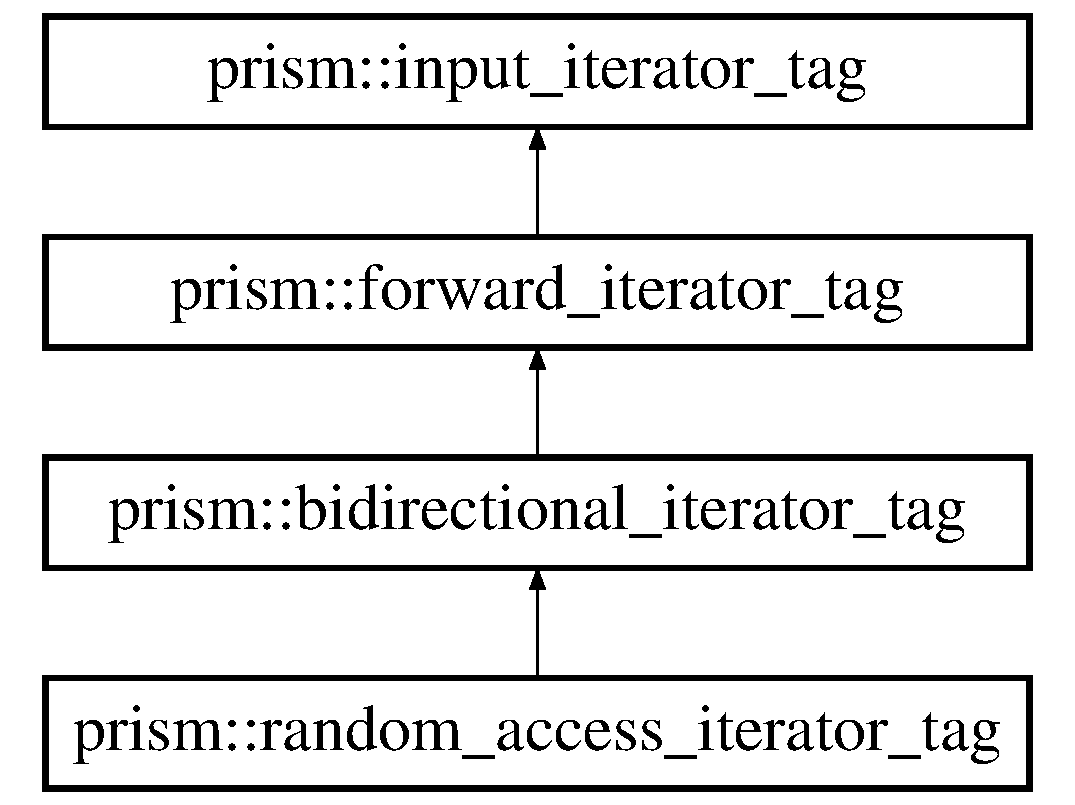
\includegraphics[height=4.000000cm]{structprism_1_1bidirectional__iterator__tag}
\end{center}
\end{figure}


The documentation for this struct was generated from the following file\+:\begin{DoxyCompactItemize}
\item 
\hyperlink{iterator__tags_8h}{iterator\+\_\+tags.\+h}\end{DoxyCompactItemize}

\hypertarget{classprism_1_1_binary_search_tree}{}\section{prism\+:\+:Binary\+Search\+Tree$<$ Key, Value, Compare, Allocator $>$ Class Template Reference}
\label{classprism_1_1_binary_search_tree}\index{prism\+::\+Binary\+Search\+Tree$<$ Key, Value, Compare, Allocator $>$@{prism\+::\+Binary\+Search\+Tree$<$ Key, Value, Compare, Allocator $>$}}
Inheritance diagram for prism\+:\+:Binary\+Search\+Tree$<$ Key, Value, Compare, Allocator $>$\+:\begin{figure}[H]
\begin{center}
\leavevmode
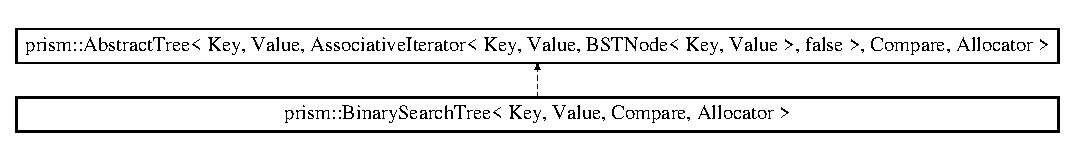
\includegraphics[height=1.544828cm]{classprism_1_1_binary_search_tree}
\end{center}
\end{figure}
\subsection*{Public Types}
\begin{DoxyCompactItemize}
\item 
typedef \hyperlink{structprism_1_1_associative_iterator}{Associative\+Iterator}$<$ Key, Value, \hyperlink{structprism_1_1_b_s_t_node}{Node}, false $>$ \hyperlink{classprism_1_1_binary_search_tree_a8c8deaa4e3617d5833c20970ffaa0348}{iterator}
\item 
typedef \hyperlink{structprism_1_1_associative_iterator}{Associative\+Iterator}$<$ Key, Value, \hyperlink{structprism_1_1_b_s_t_node}{Node}, true $>$ \hyperlink{classprism_1_1_binary_search_tree_ae72115785a3c50de35a62aa5ef102afd}{const\+\_\+iterator}
\item 
typedef Value $\ast$ \hyperlink{classprism_1_1_binary_search_tree_a159239eef3483ff85766b65e3cc8b36a}{pointer}
\item 
typedef const Value $\ast$ \hyperlink{classprism_1_1_binary_search_tree_a165bd59f5169479a5208e1c746943e2e}{const\+\_\+pointer}
\item 
typedef Value \& \hyperlink{classprism_1_1_binary_search_tree_ab924eeab8b8ce1edf77d02bceec9d4eb}{reference}
\item 
typedef const Value \& \hyperlink{classprism_1_1_binary_search_tree_aab75e547e4f5dd8e7f1518ec7b200937}{const\+\_\+reference}
\item 
typedef std\+::ptrdiff\+\_\+t \hyperlink{classprism_1_1_binary_search_tree_a9f97bb0b22c20eb1f8aff1719ad0e795}{difference\+\_\+type}
\item 
typedef std\+::size\+\_\+t \hyperlink{classprism_1_1_binary_search_tree_a757953cb7af54c9b07cf8a8a0fecb58f}{size\+\_\+type}
\end{DoxyCompactItemize}
\subsection*{Public Member Functions}
\begin{DoxyCompactItemize}
\item 
\hyperlink{classprism_1_1_binary_search_tree_a5aac58388c15e1b8bf15f7a18fff2027}{Binary\+Search\+Tree} ()
\item 
\hyperlink{classprism_1_1_binary_search_tree_ad8e02e707d90076bdb0de1728d22ff46}{$\sim$\+Binary\+Search\+Tree} ()
\item 
\hyperlink{classprism_1_1_binary_search_tree_a8c8deaa4e3617d5833c20970ffaa0348}{iterator} \hyperlink{classprism_1_1_binary_search_tree_af2ccdb9d334119a433ae95c747a3f150}{begin} ()
\item 
\hyperlink{classprism_1_1_binary_search_tree_a8c8deaa4e3617d5833c20970ffaa0348}{iterator} \hyperlink{classprism_1_1_binary_search_tree_afd834d15ab003394ce51010dcc93e8be}{begin} () const 
\item 
void \hyperlink{classprism_1_1_binary_search_tree_a014cbb1184b3028fdd0407301bdf6478}{clear} ()
\item 
\hyperlink{classprism_1_1_binary_search_tree_a8c8deaa4e3617d5833c20970ffaa0348}{iterator} \hyperlink{classprism_1_1_binary_search_tree_a2de56890b320d3ccbc099793cc85dc21}{end} ()
\item 
\hyperlink{classprism_1_1_binary_search_tree_a8c8deaa4e3617d5833c20970ffaa0348}{iterator} \hyperlink{classprism_1_1_binary_search_tree_abbdcd3785b09b1cd48b59f4105738f39}{end} () const 
\item 
void \hyperlink{classprism_1_1_binary_search_tree_a4c48d5b2002d877b7b4e4c0d52e4ed4b}{erase} (const\+\_\+key\+\_\+reference key)
\item 
const bool \hyperlink{classprism_1_1_binary_search_tree_aa9901f5ab3c87a79ed21d39691039061}{empty} () const 
\item 
\hyperlink{classprism_1_1_binary_search_tree_a8c8deaa4e3617d5833c20970ffaa0348}{iterator} \hyperlink{classprism_1_1_binary_search_tree_ae00a5f2d879ba5c08ff024c27c34d055}{find} (const\+\_\+key\+\_\+reference key) const 
\item 
\hyperlink{classprism_1_1_binary_search_tree_a8c8deaa4e3617d5833c20970ffaa0348}{iterator} \hyperlink{classprism_1_1_binary_search_tree_a223c125c5803c543281606c576cc3246}{insert} (const\+\_\+key\+\_\+reference key, \hyperlink{classprism_1_1_binary_search_tree_aab75e547e4f5dd8e7f1518ec7b200937}{const\+\_\+reference} value)
\item 
\hyperlink{classprism_1_1_binary_search_tree_a8c8deaa4e3617d5833c20970ffaa0348}{iterator} \hyperlink{classprism_1_1_binary_search_tree_a554c8ebabcfc2e8fb69eaad905674f81}{insert\+Unique} (const\+\_\+key\+\_\+reference key, \hyperlink{classprism_1_1_binary_search_tree_aab75e547e4f5dd8e7f1518ec7b200937}{const\+\_\+reference} value)
\item 
Compare \hyperlink{classprism_1_1_binary_search_tree_a831a0ec78298eaea3a3efbee3f18566b}{key\+Compare} () const 
\item 
\hyperlink{classprism_1_1_binary_search_tree_a8c8deaa4e3617d5833c20970ffaa0348}{iterator} \hyperlink{classprism_1_1_binary_search_tree_aa176caaa5c5c5951cfc7ec428cf3a7b5}{lower\+Bound} (const\+\_\+key\+\_\+reference key) const 
\item 
const int \hyperlink{classprism_1_1_binary_search_tree_a6e6aa18d300c4f4cdfa121e492684b15}{size} () const 
\item 
\hyperlink{classprism_1_1_binary_search_tree_a8c8deaa4e3617d5833c20970ffaa0348}{iterator} \hyperlink{classprism_1_1_binary_search_tree_a1146631a434b05a0846d4386b2cdf874}{upper\+Bound} (const\+\_\+key\+\_\+reference key) const 
\item 
\hyperlink{classprism_1_1_binary_search_tree_ab924eeab8b8ce1edf77d02bceec9d4eb}{reference} \hyperlink{classprism_1_1_binary_search_tree_a16c3d829f1e459e49ce0cbd31eae23c6}{operator\mbox{[}$\,$\mbox{]}} (const\+\_\+key\+\_\+reference key)
\end{DoxyCompactItemize}
\subsection*{Public Attributes}
\begin{DoxyCompactItemize}
\item 
\hyperlink{structprism_1_1_b_s_t_data}{Data} $\ast$ \hyperlink{classprism_1_1_binary_search_tree_a6d5900a993bfceb52af558fa5de72bcd}{d}
\end{DoxyCompactItemize}
\subsection*{Friends}
\begin{DoxyCompactItemize}
\item 
std\+::ostream \& \hyperlink{classprism_1_1_binary_search_tree_a3ad0aca4742a5661aad32577e6f0ceb3}{operator$<$$<$} (std\+::ostream \&out, const \hyperlink{classprism_1_1_binary_search_tree}{Binary\+Search\+Tree}$<$ Key, Value, Compare, \hyperlink{classprism_1_1_allocator}{Allocator} $>$ \&t)
\end{DoxyCompactItemize}
\subsection*{Additional Inherited Members}


\subsection{Member Typedef Documentation}
\index{prism\+::\+Binary\+Search\+Tree@{prism\+::\+Binary\+Search\+Tree}!const\+\_\+iterator@{const\+\_\+iterator}}
\index{const\+\_\+iterator@{const\+\_\+iterator}!prism\+::\+Binary\+Search\+Tree@{prism\+::\+Binary\+Search\+Tree}}
\subsubsection[{\texorpdfstring{const\+\_\+iterator}{const_iterator}}]{\setlength{\rightskip}{0pt plus 5cm}template$<$class Key , class Value , class Compare  = prism\+::less$<$\+Key$>$, class Allocator  = prism\+::\+Allocator$<$prism\+::pair$<$\+Key,\+Value$>$$>$$>$ typedef {\bf Associative\+Iterator}$<$Key,Value,{\bf Node},true$>$ {\bf prism\+::\+Binary\+Search\+Tree}$<$ Key, Value, Compare, {\bf Allocator} $>$\+::{\bf const\+\_\+iterator}}\hypertarget{classprism_1_1_binary_search_tree_ae72115785a3c50de35a62aa5ef102afd}{}\label{classprism_1_1_binary_search_tree_ae72115785a3c50de35a62aa5ef102afd}
\index{prism\+::\+Binary\+Search\+Tree@{prism\+::\+Binary\+Search\+Tree}!const\+\_\+pointer@{const\+\_\+pointer}}
\index{const\+\_\+pointer@{const\+\_\+pointer}!prism\+::\+Binary\+Search\+Tree@{prism\+::\+Binary\+Search\+Tree}}
\subsubsection[{\texorpdfstring{const\+\_\+pointer}{const_pointer}}]{\setlength{\rightskip}{0pt plus 5cm}template$<$class Key , class Value , class Compare  = prism\+::less$<$\+Key$>$, class Allocator  = prism\+::\+Allocator$<$prism\+::pair$<$\+Key,\+Value$>$$>$$>$ typedef const Value$\ast$ {\bf prism\+::\+Binary\+Search\+Tree}$<$ Key, Value, Compare, {\bf Allocator} $>$\+::{\bf const\+\_\+pointer}}\hypertarget{classprism_1_1_binary_search_tree_a165bd59f5169479a5208e1c746943e2e}{}\label{classprism_1_1_binary_search_tree_a165bd59f5169479a5208e1c746943e2e}
\index{prism\+::\+Binary\+Search\+Tree@{prism\+::\+Binary\+Search\+Tree}!const\+\_\+reference@{const\+\_\+reference}}
\index{const\+\_\+reference@{const\+\_\+reference}!prism\+::\+Binary\+Search\+Tree@{prism\+::\+Binary\+Search\+Tree}}
\subsubsection[{\texorpdfstring{const\+\_\+reference}{const_reference}}]{\setlength{\rightskip}{0pt plus 5cm}template$<$class Key , class Value , class Compare  = prism\+::less$<$\+Key$>$, class Allocator  = prism\+::\+Allocator$<$prism\+::pair$<$\+Key,\+Value$>$$>$$>$ typedef const Value\& {\bf prism\+::\+Binary\+Search\+Tree}$<$ Key, Value, Compare, {\bf Allocator} $>$\+::{\bf const\+\_\+reference}}\hypertarget{classprism_1_1_binary_search_tree_aab75e547e4f5dd8e7f1518ec7b200937}{}\label{classprism_1_1_binary_search_tree_aab75e547e4f5dd8e7f1518ec7b200937}
\index{prism\+::\+Binary\+Search\+Tree@{prism\+::\+Binary\+Search\+Tree}!difference\+\_\+type@{difference\+\_\+type}}
\index{difference\+\_\+type@{difference\+\_\+type}!prism\+::\+Binary\+Search\+Tree@{prism\+::\+Binary\+Search\+Tree}}
\subsubsection[{\texorpdfstring{difference\+\_\+type}{difference_type}}]{\setlength{\rightskip}{0pt plus 5cm}template$<$class Key , class Value , class Compare  = prism\+::less$<$\+Key$>$, class Allocator  = prism\+::\+Allocator$<$prism\+::pair$<$\+Key,\+Value$>$$>$$>$ typedef std\+::ptrdiff\+\_\+t {\bf prism\+::\+Binary\+Search\+Tree}$<$ Key, Value, Compare, {\bf Allocator} $>$\+::{\bf difference\+\_\+type}}\hypertarget{classprism_1_1_binary_search_tree_a9f97bb0b22c20eb1f8aff1719ad0e795}{}\label{classprism_1_1_binary_search_tree_a9f97bb0b22c20eb1f8aff1719ad0e795}
\index{prism\+::\+Binary\+Search\+Tree@{prism\+::\+Binary\+Search\+Tree}!iterator@{iterator}}
\index{iterator@{iterator}!prism\+::\+Binary\+Search\+Tree@{prism\+::\+Binary\+Search\+Tree}}
\subsubsection[{\texorpdfstring{iterator}{iterator}}]{\setlength{\rightskip}{0pt plus 5cm}template$<$class Key , class Value , class Compare  = prism\+::less$<$\+Key$>$, class Allocator  = prism\+::\+Allocator$<$prism\+::pair$<$\+Key,\+Value$>$$>$$>$ typedef {\bf Associative\+Iterator}$<$Key,Value,{\bf Node},false$>$ {\bf prism\+::\+Binary\+Search\+Tree}$<$ Key, Value, Compare, {\bf Allocator} $>$\+::{\bf iterator}}\hypertarget{classprism_1_1_binary_search_tree_a8c8deaa4e3617d5833c20970ffaa0348}{}\label{classprism_1_1_binary_search_tree_a8c8deaa4e3617d5833c20970ffaa0348}
\index{prism\+::\+Binary\+Search\+Tree@{prism\+::\+Binary\+Search\+Tree}!pointer@{pointer}}
\index{pointer@{pointer}!prism\+::\+Binary\+Search\+Tree@{prism\+::\+Binary\+Search\+Tree}}
\subsubsection[{\texorpdfstring{pointer}{pointer}}]{\setlength{\rightskip}{0pt plus 5cm}template$<$class Key , class Value , class Compare  = prism\+::less$<$\+Key$>$, class Allocator  = prism\+::\+Allocator$<$prism\+::pair$<$\+Key,\+Value$>$$>$$>$ typedef Value$\ast$ {\bf prism\+::\+Binary\+Search\+Tree}$<$ Key, Value, Compare, {\bf Allocator} $>$\+::{\bf pointer}}\hypertarget{classprism_1_1_binary_search_tree_a159239eef3483ff85766b65e3cc8b36a}{}\label{classprism_1_1_binary_search_tree_a159239eef3483ff85766b65e3cc8b36a}
\index{prism\+::\+Binary\+Search\+Tree@{prism\+::\+Binary\+Search\+Tree}!reference@{reference}}
\index{reference@{reference}!prism\+::\+Binary\+Search\+Tree@{prism\+::\+Binary\+Search\+Tree}}
\subsubsection[{\texorpdfstring{reference}{reference}}]{\setlength{\rightskip}{0pt plus 5cm}template$<$class Key , class Value , class Compare  = prism\+::less$<$\+Key$>$, class Allocator  = prism\+::\+Allocator$<$prism\+::pair$<$\+Key,\+Value$>$$>$$>$ typedef Value\& {\bf prism\+::\+Binary\+Search\+Tree}$<$ Key, Value, Compare, {\bf Allocator} $>$\+::{\bf reference}}\hypertarget{classprism_1_1_binary_search_tree_ab924eeab8b8ce1edf77d02bceec9d4eb}{}\label{classprism_1_1_binary_search_tree_ab924eeab8b8ce1edf77d02bceec9d4eb}
\index{prism\+::\+Binary\+Search\+Tree@{prism\+::\+Binary\+Search\+Tree}!size\+\_\+type@{size\+\_\+type}}
\index{size\+\_\+type@{size\+\_\+type}!prism\+::\+Binary\+Search\+Tree@{prism\+::\+Binary\+Search\+Tree}}
\subsubsection[{\texorpdfstring{size\+\_\+type}{size_type}}]{\setlength{\rightskip}{0pt plus 5cm}template$<$class Key , class Value , class Compare  = prism\+::less$<$\+Key$>$, class Allocator  = prism\+::\+Allocator$<$prism\+::pair$<$\+Key,\+Value$>$$>$$>$ typedef std\+::size\+\_\+t {\bf prism\+::\+Binary\+Search\+Tree}$<$ Key, Value, Compare, {\bf Allocator} $>$\+::{\bf size\+\_\+type}}\hypertarget{classprism_1_1_binary_search_tree_a757953cb7af54c9b07cf8a8a0fecb58f}{}\label{classprism_1_1_binary_search_tree_a757953cb7af54c9b07cf8a8a0fecb58f}


\subsection{Constructor \& Destructor Documentation}
\index{prism\+::\+Binary\+Search\+Tree@{prism\+::\+Binary\+Search\+Tree}!Binary\+Search\+Tree@{Binary\+Search\+Tree}}
\index{Binary\+Search\+Tree@{Binary\+Search\+Tree}!prism\+::\+Binary\+Search\+Tree@{prism\+::\+Binary\+Search\+Tree}}
\subsubsection[{\texorpdfstring{Binary\+Search\+Tree()}{BinarySearchTree()}}]{\setlength{\rightskip}{0pt plus 5cm}template$<$class Key , class Value , class Compare  = prism\+::less$<$\+Key$>$, class Allocator  = prism\+::\+Allocator$<$prism\+::pair$<$\+Key,\+Value$>$$>$$>$ {\bf prism\+::\+Binary\+Search\+Tree}$<$ Key, Value, Compare, {\bf Allocator} $>$\+::{\bf Binary\+Search\+Tree} (
\begin{DoxyParamCaption}
{}
\end{DoxyParamCaption}
)\hspace{0.3cm}{\ttfamily [inline]}}\hypertarget{classprism_1_1_binary_search_tree_a5aac58388c15e1b8bf15f7a18fff2027}{}\label{classprism_1_1_binary_search_tree_a5aac58388c15e1b8bf15f7a18fff2027}
\index{prism\+::\+Binary\+Search\+Tree@{prism\+::\+Binary\+Search\+Tree}!````~Binary\+Search\+Tree@{$\sim$\+Binary\+Search\+Tree}}
\index{````~Binary\+Search\+Tree@{$\sim$\+Binary\+Search\+Tree}!prism\+::\+Binary\+Search\+Tree@{prism\+::\+Binary\+Search\+Tree}}
\subsubsection[{\texorpdfstring{$\sim$\+Binary\+Search\+Tree()}{~BinarySearchTree()}}]{\setlength{\rightskip}{0pt plus 5cm}template$<$class Key , class Value , class Compare  = prism\+::less$<$\+Key$>$, class Allocator  = prism\+::\+Allocator$<$prism\+::pair$<$\+Key,\+Value$>$$>$$>$ {\bf prism\+::\+Binary\+Search\+Tree}$<$ Key, Value, Compare, {\bf Allocator} $>$\+::$\sim${\bf Binary\+Search\+Tree} (
\begin{DoxyParamCaption}
{}
\end{DoxyParamCaption}
)\hspace{0.3cm}{\ttfamily [inline]}}\hypertarget{classprism_1_1_binary_search_tree_ad8e02e707d90076bdb0de1728d22ff46}{}\label{classprism_1_1_binary_search_tree_ad8e02e707d90076bdb0de1728d22ff46}


\subsection{Member Function Documentation}
\index{prism\+::\+Binary\+Search\+Tree@{prism\+::\+Binary\+Search\+Tree}!begin@{begin}}
\index{begin@{begin}!prism\+::\+Binary\+Search\+Tree@{prism\+::\+Binary\+Search\+Tree}}
\subsubsection[{\texorpdfstring{begin()}{begin()}}]{\setlength{\rightskip}{0pt plus 5cm}template$<$class Key , class Value , class Compare  = prism\+::less$<$\+Key$>$, class Allocator  = prism\+::\+Allocator$<$prism\+::pair$<$\+Key,\+Value$>$$>$$>$ {\bf iterator} {\bf prism\+::\+Binary\+Search\+Tree}$<$ Key, Value, Compare, {\bf Allocator} $>$\+::begin (
\begin{DoxyParamCaption}
{}
\end{DoxyParamCaption}
)\hspace{0.3cm}{\ttfamily [inline]}, {\ttfamily [virtual]}}\hypertarget{classprism_1_1_binary_search_tree_af2ccdb9d334119a433ae95c747a3f150}{}\label{classprism_1_1_binary_search_tree_af2ccdb9d334119a433ae95c747a3f150}


Implements \hyperlink{classprism_1_1_abstract_tree_a8e03e5f6793880f0da7eaf55d6711d86}{prism\+::\+Abstract\+Tree$<$ Key, Value, Associative\+Iterator$<$ Key, Value, B\+S\+T\+Node$<$ Key, Value $>$, false $>$, Compare, Allocator $>$}.

\index{prism\+::\+Binary\+Search\+Tree@{prism\+::\+Binary\+Search\+Tree}!begin@{begin}}
\index{begin@{begin}!prism\+::\+Binary\+Search\+Tree@{prism\+::\+Binary\+Search\+Tree}}
\subsubsection[{\texorpdfstring{begin() const }{begin() const }}]{\setlength{\rightskip}{0pt plus 5cm}template$<$class Key , class Value , class Compare  = prism\+::less$<$\+Key$>$, class Allocator  = prism\+::\+Allocator$<$prism\+::pair$<$\+Key,\+Value$>$$>$$>$ {\bf iterator} {\bf prism\+::\+Binary\+Search\+Tree}$<$ Key, Value, Compare, {\bf Allocator} $>$\+::begin (
\begin{DoxyParamCaption}
{}
\end{DoxyParamCaption}
) const\hspace{0.3cm}{\ttfamily [inline]}, {\ttfamily [virtual]}}\hypertarget{classprism_1_1_binary_search_tree_afd834d15ab003394ce51010dcc93e8be}{}\label{classprism_1_1_binary_search_tree_afd834d15ab003394ce51010dcc93e8be}


Implements \hyperlink{classprism_1_1_abstract_tree_ae15b25cf84fa19e02965ce93d8ff6475}{prism\+::\+Abstract\+Tree$<$ Key, Value, Associative\+Iterator$<$ Key, Value, B\+S\+T\+Node$<$ Key, Value $>$, false $>$, Compare, Allocator $>$}.

\index{prism\+::\+Binary\+Search\+Tree@{prism\+::\+Binary\+Search\+Tree}!clear@{clear}}
\index{clear@{clear}!prism\+::\+Binary\+Search\+Tree@{prism\+::\+Binary\+Search\+Tree}}
\subsubsection[{\texorpdfstring{clear()}{clear()}}]{\setlength{\rightskip}{0pt plus 5cm}template$<$class Key , class Value , class Compare  = prism\+::less$<$\+Key$>$, class Allocator  = prism\+::\+Allocator$<$prism\+::pair$<$\+Key,\+Value$>$$>$$>$ void {\bf prism\+::\+Binary\+Search\+Tree}$<$ Key, Value, Compare, {\bf Allocator} $>$\+::clear (
\begin{DoxyParamCaption}
{}
\end{DoxyParamCaption}
)\hspace{0.3cm}{\ttfamily [inline]}, {\ttfamily [virtual]}}\hypertarget{classprism_1_1_binary_search_tree_a014cbb1184b3028fdd0407301bdf6478}{}\label{classprism_1_1_binary_search_tree_a014cbb1184b3028fdd0407301bdf6478}


Implements \hyperlink{classprism_1_1_abstract_tree_a6c286774c61d70e75d4897b989bc4be0}{prism\+::\+Abstract\+Tree$<$ Key, Value, Associative\+Iterator$<$ Key, Value, B\+S\+T\+Node$<$ Key, Value $>$, false $>$, Compare, Allocator $>$}.

\index{prism\+::\+Binary\+Search\+Tree@{prism\+::\+Binary\+Search\+Tree}!empty@{empty}}
\index{empty@{empty}!prism\+::\+Binary\+Search\+Tree@{prism\+::\+Binary\+Search\+Tree}}
\subsubsection[{\texorpdfstring{empty() const }{empty() const }}]{\setlength{\rightskip}{0pt plus 5cm}template$<$class Key , class Value , class Compare  = prism\+::less$<$\+Key$>$, class Allocator  = prism\+::\+Allocator$<$prism\+::pair$<$\+Key,\+Value$>$$>$$>$ const bool {\bf prism\+::\+Binary\+Search\+Tree}$<$ Key, Value, Compare, {\bf Allocator} $>$\+::empty (
\begin{DoxyParamCaption}
{}
\end{DoxyParamCaption}
) const\hspace{0.3cm}{\ttfamily [inline]}, {\ttfamily [virtual]}}\hypertarget{classprism_1_1_binary_search_tree_aa9901f5ab3c87a79ed21d39691039061}{}\label{classprism_1_1_binary_search_tree_aa9901f5ab3c87a79ed21d39691039061}


Implements \hyperlink{classprism_1_1_abstract_tree_a49bb10ec57e7601c000ccf8a627595e4}{prism\+::\+Abstract\+Tree$<$ Key, Value, Associative\+Iterator$<$ Key, Value, B\+S\+T\+Node$<$ Key, Value $>$, false $>$, Compare, Allocator $>$}.

\index{prism\+::\+Binary\+Search\+Tree@{prism\+::\+Binary\+Search\+Tree}!end@{end}}
\index{end@{end}!prism\+::\+Binary\+Search\+Tree@{prism\+::\+Binary\+Search\+Tree}}
\subsubsection[{\texorpdfstring{end()}{end()}}]{\setlength{\rightskip}{0pt plus 5cm}template$<$class Key , class Value , class Compare  = prism\+::less$<$\+Key$>$, class Allocator  = prism\+::\+Allocator$<$prism\+::pair$<$\+Key,\+Value$>$$>$$>$ {\bf iterator} {\bf prism\+::\+Binary\+Search\+Tree}$<$ Key, Value, Compare, {\bf Allocator} $>$\+::end (
\begin{DoxyParamCaption}
{}
\end{DoxyParamCaption}
)\hspace{0.3cm}{\ttfamily [inline]}, {\ttfamily [virtual]}}\hypertarget{classprism_1_1_binary_search_tree_a2de56890b320d3ccbc099793cc85dc21}{}\label{classprism_1_1_binary_search_tree_a2de56890b320d3ccbc099793cc85dc21}


Implements \hyperlink{classprism_1_1_abstract_tree_ac167d15fc84a60ae9bec6a2bec0ee883}{prism\+::\+Abstract\+Tree$<$ Key, Value, Associative\+Iterator$<$ Key, Value, B\+S\+T\+Node$<$ Key, Value $>$, false $>$, Compare, Allocator $>$}.

\index{prism\+::\+Binary\+Search\+Tree@{prism\+::\+Binary\+Search\+Tree}!end@{end}}
\index{end@{end}!prism\+::\+Binary\+Search\+Tree@{prism\+::\+Binary\+Search\+Tree}}
\subsubsection[{\texorpdfstring{end() const }{end() const }}]{\setlength{\rightskip}{0pt plus 5cm}template$<$class Key , class Value , class Compare  = prism\+::less$<$\+Key$>$, class Allocator  = prism\+::\+Allocator$<$prism\+::pair$<$\+Key,\+Value$>$$>$$>$ {\bf iterator} {\bf prism\+::\+Binary\+Search\+Tree}$<$ Key, Value, Compare, {\bf Allocator} $>$\+::end (
\begin{DoxyParamCaption}
{}
\end{DoxyParamCaption}
) const\hspace{0.3cm}{\ttfamily [inline]}, {\ttfamily [virtual]}}\hypertarget{classprism_1_1_binary_search_tree_abbdcd3785b09b1cd48b59f4105738f39}{}\label{classprism_1_1_binary_search_tree_abbdcd3785b09b1cd48b59f4105738f39}


Implements \hyperlink{classprism_1_1_abstract_tree_a104a30a25913fe65b12dc2dbf645ae5a}{prism\+::\+Abstract\+Tree$<$ Key, Value, Associative\+Iterator$<$ Key, Value, B\+S\+T\+Node$<$ Key, Value $>$, false $>$, Compare, Allocator $>$}.

\index{prism\+::\+Binary\+Search\+Tree@{prism\+::\+Binary\+Search\+Tree}!erase@{erase}}
\index{erase@{erase}!prism\+::\+Binary\+Search\+Tree@{prism\+::\+Binary\+Search\+Tree}}
\subsubsection[{\texorpdfstring{erase(const\+\_\+key\+\_\+reference key)}{erase(const_key_reference key)}}]{\setlength{\rightskip}{0pt plus 5cm}template$<$class Key , class Value , class Compare  = prism\+::less$<$\+Key$>$, class Allocator  = prism\+::\+Allocator$<$prism\+::pair$<$\+Key,\+Value$>$$>$$>$ void {\bf prism\+::\+Binary\+Search\+Tree}$<$ Key, Value, Compare, {\bf Allocator} $>$\+::erase (
\begin{DoxyParamCaption}
\item[{const\+\_\+key\+\_\+reference}]{key}
\end{DoxyParamCaption}
)\hspace{0.3cm}{\ttfamily [inline]}}\hypertarget{classprism_1_1_binary_search_tree_a4c48d5b2002d877b7b4e4c0d52e4ed4b}{}\label{classprism_1_1_binary_search_tree_a4c48d5b2002d877b7b4e4c0d52e4ed4b}
\index{prism\+::\+Binary\+Search\+Tree@{prism\+::\+Binary\+Search\+Tree}!find@{find}}
\index{find@{find}!prism\+::\+Binary\+Search\+Tree@{prism\+::\+Binary\+Search\+Tree}}
\subsubsection[{\texorpdfstring{find(const\+\_\+key\+\_\+reference key) const }{find(const_key_reference key) const }}]{\setlength{\rightskip}{0pt plus 5cm}template$<$class Key , class Value , class Compare  = prism\+::less$<$\+Key$>$, class Allocator  = prism\+::\+Allocator$<$prism\+::pair$<$\+Key,\+Value$>$$>$$>$ {\bf iterator} {\bf prism\+::\+Binary\+Search\+Tree}$<$ Key, Value, Compare, {\bf Allocator} $>$\+::find (
\begin{DoxyParamCaption}
\item[{const\+\_\+key\+\_\+reference}]{key}
\end{DoxyParamCaption}
) const\hspace{0.3cm}{\ttfamily [inline]}}\hypertarget{classprism_1_1_binary_search_tree_ae00a5f2d879ba5c08ff024c27c34d055}{}\label{classprism_1_1_binary_search_tree_ae00a5f2d879ba5c08ff024c27c34d055}
\index{prism\+::\+Binary\+Search\+Tree@{prism\+::\+Binary\+Search\+Tree}!insert@{insert}}
\index{insert@{insert}!prism\+::\+Binary\+Search\+Tree@{prism\+::\+Binary\+Search\+Tree}}
\subsubsection[{\texorpdfstring{insert(const\+\_\+key\+\_\+reference key, const\+\_\+reference value)}{insert(const_key_reference key, const_reference value)}}]{\setlength{\rightskip}{0pt plus 5cm}template$<$class Key , class Value , class Compare  = prism\+::less$<$\+Key$>$, class Allocator  = prism\+::\+Allocator$<$prism\+::pair$<$\+Key,\+Value$>$$>$$>$ {\bf iterator} {\bf prism\+::\+Binary\+Search\+Tree}$<$ Key, Value, Compare, {\bf Allocator} $>$\+::insert (
\begin{DoxyParamCaption}
\item[{const\+\_\+key\+\_\+reference}]{key, }
\item[{{\bf const\+\_\+reference}}]{value}
\end{DoxyParamCaption}
)\hspace{0.3cm}{\ttfamily [inline]}}\hypertarget{classprism_1_1_binary_search_tree_a223c125c5803c543281606c576cc3246}{}\label{classprism_1_1_binary_search_tree_a223c125c5803c543281606c576cc3246}
\index{prism\+::\+Binary\+Search\+Tree@{prism\+::\+Binary\+Search\+Tree}!insert\+Unique@{insert\+Unique}}
\index{insert\+Unique@{insert\+Unique}!prism\+::\+Binary\+Search\+Tree@{prism\+::\+Binary\+Search\+Tree}}
\subsubsection[{\texorpdfstring{insert\+Unique(const\+\_\+key\+\_\+reference key, const\+\_\+reference value)}{insertUnique(const_key_reference key, const_reference value)}}]{\setlength{\rightskip}{0pt plus 5cm}template$<$class Key , class Value , class Compare  = prism\+::less$<$\+Key$>$, class Allocator  = prism\+::\+Allocator$<$prism\+::pair$<$\+Key,\+Value$>$$>$$>$ {\bf iterator} {\bf prism\+::\+Binary\+Search\+Tree}$<$ Key, Value, Compare, {\bf Allocator} $>$\+::insert\+Unique (
\begin{DoxyParamCaption}
\item[{const\+\_\+key\+\_\+reference}]{key, }
\item[{{\bf const\+\_\+reference}}]{value}
\end{DoxyParamCaption}
)\hspace{0.3cm}{\ttfamily [inline]}}\hypertarget{classprism_1_1_binary_search_tree_a554c8ebabcfc2e8fb69eaad905674f81}{}\label{classprism_1_1_binary_search_tree_a554c8ebabcfc2e8fb69eaad905674f81}
\index{prism\+::\+Binary\+Search\+Tree@{prism\+::\+Binary\+Search\+Tree}!key\+Compare@{key\+Compare}}
\index{key\+Compare@{key\+Compare}!prism\+::\+Binary\+Search\+Tree@{prism\+::\+Binary\+Search\+Tree}}
\subsubsection[{\texorpdfstring{key\+Compare() const }{keyCompare() const }}]{\setlength{\rightskip}{0pt plus 5cm}template$<$class Key , class Value , class Compare  = prism\+::less$<$\+Key$>$, class Allocator  = prism\+::\+Allocator$<$prism\+::pair$<$\+Key,\+Value$>$$>$$>$ Compare {\bf prism\+::\+Binary\+Search\+Tree}$<$ Key, Value, Compare, {\bf Allocator} $>$\+::key\+Compare (
\begin{DoxyParamCaption}
{}
\end{DoxyParamCaption}
) const\hspace{0.3cm}{\ttfamily [inline]}, {\ttfamily [virtual]}}\hypertarget{classprism_1_1_binary_search_tree_a831a0ec78298eaea3a3efbee3f18566b}{}\label{classprism_1_1_binary_search_tree_a831a0ec78298eaea3a3efbee3f18566b}


Implements \hyperlink{classprism_1_1_abstract_tree_ae67686bf3cfd721c038d8f22f5f157b6}{prism\+::\+Abstract\+Tree$<$ Key, Value, Associative\+Iterator$<$ Key, Value, B\+S\+T\+Node$<$ Key, Value $>$, false $>$, Compare, Allocator $>$}.

\index{prism\+::\+Binary\+Search\+Tree@{prism\+::\+Binary\+Search\+Tree}!lower\+Bound@{lower\+Bound}}
\index{lower\+Bound@{lower\+Bound}!prism\+::\+Binary\+Search\+Tree@{prism\+::\+Binary\+Search\+Tree}}
\subsubsection[{\texorpdfstring{lower\+Bound(const\+\_\+key\+\_\+reference key) const }{lowerBound(const_key_reference key) const }}]{\setlength{\rightskip}{0pt plus 5cm}template$<$class Key , class Value , class Compare  = prism\+::less$<$\+Key$>$, class Allocator  = prism\+::\+Allocator$<$prism\+::pair$<$\+Key,\+Value$>$$>$$>$ {\bf iterator} {\bf prism\+::\+Binary\+Search\+Tree}$<$ Key, Value, Compare, {\bf Allocator} $>$\+::lower\+Bound (
\begin{DoxyParamCaption}
\item[{const\+\_\+key\+\_\+reference}]{key}
\end{DoxyParamCaption}
) const\hspace{0.3cm}{\ttfamily [inline]}}\hypertarget{classprism_1_1_binary_search_tree_aa176caaa5c5c5951cfc7ec428cf3a7b5}{}\label{classprism_1_1_binary_search_tree_aa176caaa5c5c5951cfc7ec428cf3a7b5}
\index{prism\+::\+Binary\+Search\+Tree@{prism\+::\+Binary\+Search\+Tree}!operator\mbox{[}$\,$\mbox{]}@{operator[]}}
\index{operator\mbox{[}$\,$\mbox{]}@{operator[]}!prism\+::\+Binary\+Search\+Tree@{prism\+::\+Binary\+Search\+Tree}}
\subsubsection[{\texorpdfstring{operator[](const\+\_\+key\+\_\+reference key)}{operator[](const_key_reference key)}}]{\setlength{\rightskip}{0pt plus 5cm}template$<$class Key , class Value , class Compare  = prism\+::less$<$\+Key$>$, class Allocator  = prism\+::\+Allocator$<$prism\+::pair$<$\+Key,\+Value$>$$>$$>$ {\bf reference} {\bf prism\+::\+Binary\+Search\+Tree}$<$ Key, Value, Compare, {\bf Allocator} $>$\+::operator\mbox{[}$\,$\mbox{]} (
\begin{DoxyParamCaption}
\item[{const\+\_\+key\+\_\+reference}]{key}
\end{DoxyParamCaption}
)\hspace{0.3cm}{\ttfamily [inline]}}\hypertarget{classprism_1_1_binary_search_tree_a16c3d829f1e459e49ce0cbd31eae23c6}{}\label{classprism_1_1_binary_search_tree_a16c3d829f1e459e49ce0cbd31eae23c6}
\index{prism\+::\+Binary\+Search\+Tree@{prism\+::\+Binary\+Search\+Tree}!size@{size}}
\index{size@{size}!prism\+::\+Binary\+Search\+Tree@{prism\+::\+Binary\+Search\+Tree}}
\subsubsection[{\texorpdfstring{size() const }{size() const }}]{\setlength{\rightskip}{0pt plus 5cm}template$<$class Key , class Value , class Compare  = prism\+::less$<$\+Key$>$, class Allocator  = prism\+::\+Allocator$<$prism\+::pair$<$\+Key,\+Value$>$$>$$>$ const int {\bf prism\+::\+Binary\+Search\+Tree}$<$ Key, Value, Compare, {\bf Allocator} $>$\+::size (
\begin{DoxyParamCaption}
{}
\end{DoxyParamCaption}
) const\hspace{0.3cm}{\ttfamily [inline]}, {\ttfamily [virtual]}}\hypertarget{classprism_1_1_binary_search_tree_a6e6aa18d300c4f4cdfa121e492684b15}{}\label{classprism_1_1_binary_search_tree_a6e6aa18d300c4f4cdfa121e492684b15}


Implements \hyperlink{classprism_1_1_abstract_tree_adab50475261a20c17d4dcc772e294b38}{prism\+::\+Abstract\+Tree$<$ Key, Value, Associative\+Iterator$<$ Key, Value, B\+S\+T\+Node$<$ Key, Value $>$, false $>$, Compare, Allocator $>$}.

\index{prism\+::\+Binary\+Search\+Tree@{prism\+::\+Binary\+Search\+Tree}!upper\+Bound@{upper\+Bound}}
\index{upper\+Bound@{upper\+Bound}!prism\+::\+Binary\+Search\+Tree@{prism\+::\+Binary\+Search\+Tree}}
\subsubsection[{\texorpdfstring{upper\+Bound(const\+\_\+key\+\_\+reference key) const }{upperBound(const_key_reference key) const }}]{\setlength{\rightskip}{0pt plus 5cm}template$<$class Key , class Value , class Compare  = prism\+::less$<$\+Key$>$, class Allocator  = prism\+::\+Allocator$<$prism\+::pair$<$\+Key,\+Value$>$$>$$>$ {\bf iterator} {\bf prism\+::\+Binary\+Search\+Tree}$<$ Key, Value, Compare, {\bf Allocator} $>$\+::upper\+Bound (
\begin{DoxyParamCaption}
\item[{const\+\_\+key\+\_\+reference}]{key}
\end{DoxyParamCaption}
) const\hspace{0.3cm}{\ttfamily [inline]}}\hypertarget{classprism_1_1_binary_search_tree_a1146631a434b05a0846d4386b2cdf874}{}\label{classprism_1_1_binary_search_tree_a1146631a434b05a0846d4386b2cdf874}


\subsection{Friends And Related Function Documentation}
\index{prism\+::\+Binary\+Search\+Tree@{prism\+::\+Binary\+Search\+Tree}!operator$<$$<$@{operator$<$$<$}}
\index{operator$<$$<$@{operator$<$$<$}!prism\+::\+Binary\+Search\+Tree@{prism\+::\+Binary\+Search\+Tree}}
\subsubsection[{\texorpdfstring{operator$<$$<$}{operator<<}}]{\setlength{\rightskip}{0pt plus 5cm}template$<$class Key , class Value , class Compare  = prism\+::less$<$\+Key$>$, class Allocator  = prism\+::\+Allocator$<$prism\+::pair$<$\+Key,\+Value$>$$>$$>$ std\+::ostream\& operator$<$$<$ (
\begin{DoxyParamCaption}
\item[{std\+::ostream \&}]{out, }
\item[{const {\bf Binary\+Search\+Tree}$<$ Key, Value, Compare, {\bf Allocator} $>$ \&}]{t}
\end{DoxyParamCaption}
)\hspace{0.3cm}{\ttfamily [friend]}}\hypertarget{classprism_1_1_binary_search_tree_a3ad0aca4742a5661aad32577e6f0ceb3}{}\label{classprism_1_1_binary_search_tree_a3ad0aca4742a5661aad32577e6f0ceb3}


\subsection{Member Data Documentation}
\index{prism\+::\+Binary\+Search\+Tree@{prism\+::\+Binary\+Search\+Tree}!d@{d}}
\index{d@{d}!prism\+::\+Binary\+Search\+Tree@{prism\+::\+Binary\+Search\+Tree}}
\subsubsection[{\texorpdfstring{d}{d}}]{\setlength{\rightskip}{0pt plus 5cm}template$<$class Key , class Value , class Compare  = prism\+::less$<$\+Key$>$, class Allocator  = prism\+::\+Allocator$<$prism\+::pair$<$\+Key,\+Value$>$$>$$>$ {\bf Data}$\ast$ {\bf prism\+::\+Binary\+Search\+Tree}$<$ Key, Value, Compare, {\bf Allocator} $>$\+::d}\hypertarget{classprism_1_1_binary_search_tree_a6d5900a993bfceb52af558fa5de72bcd}{}\label{classprism_1_1_binary_search_tree_a6d5900a993bfceb52af558fa5de72bcd}


The documentation for this class was generated from the following file\+:\begin{DoxyCompactItemize}
\item 
\hyperlink{_binary_search_tree_8h}{Binary\+Search\+Tree.\+h}\end{DoxyCompactItemize}

\hypertarget{classprism_1_1_bitvector}{}\section{prism\+:\+:Bitvector Class Reference}
\label{classprism_1_1_bitvector}\index{prism\+::\+Bitvector@{prism\+::\+Bitvector}}


{\ttfamily \#include $<$Bitvector.\+h$>$}

\subsection*{Public Member Functions}
\begin{DoxyCompactItemize}
\item 
\hyperlink{classprism_1_1_bitvector_a41d5de4bbd7bf193121a1614cf6b3b3b}{Bitvector} ()
\item 
\hyperlink{classprism_1_1_bitvector_ae2c403debb39b93d7de3317deb0daeeb}{Bitvector} (const int n\+Bits)
\item 
\hyperlink{classprism_1_1_bitvector_aaf4223cb87ea463a8f329a5599644314}{Bitvector} (const \hyperlink{classprism_1_1_string}{String} \&bit\+String)
\item 
\hyperlink{classprism_1_1_bitvector_a9b0b8f78113cbce3082f2c67fb702a6c}{Bitvector} (const \hyperlink{classprism_1_1_bitvector}{Bitvector} \&\hyperlink{namespaceprism_ae776f4cd825f79e7af1cf6ee1d90a209}{copy})
\item 
virtual \hyperlink{classprism_1_1_bitvector_ac68d7732ae33ccded5b5ef5971280c6d}{$\sim$\+Bitvector} ()
\item 
const bool \hyperlink{classprism_1_1_bitvector_a0a3d203905a1125a2afbdd928997dbe2}{get} (int bit) const 
\item 
void \hyperlink{classprism_1_1_bitvector_abdf123d4a94086c5525ce7d8eed8a6e3}{reset\+All} ()
\item 
void \hyperlink{classprism_1_1_bitvector_aaa4362884a96b180fd45dd261423a7e3}{set\+All} ()
\item 
void \hyperlink{classprism_1_1_bitvector_af6dd4b91e57bb6a95f30c55fdb1ce6a5}{set} (int bit, const bool b=true)
\item 
const int \hyperlink{classprism_1_1_bitvector_aefc31462d8a52013191e0df4f45ccae4}{size} () const 
\item 
\hyperlink{classprism_1_1_string}{String} \hyperlink{classprism_1_1_bitvector_a2639e8ad277f15e545e2ec78db17ab4c}{to\+String} () const 
\item 
\hyperlink{classprism_1_1_bitvector}{Bitvector} \hyperlink{classprism_1_1_bitvector_a0d5163be9867dee195648df83273076a}{operator$<$$<$} (const int pos) const 
\item 
\hyperlink{classprism_1_1_bitvector}{Bitvector} \hyperlink{classprism_1_1_bitvector_a8cb5d12bfecf59503a0e9d9e4bbfa0e8}{operator$>$$>$} (const int pos) const 
\item 
\hyperlink{classprism_1_1_bitvector}{Bitvector} \& \hyperlink{classprism_1_1_bitvector_acf4750aad13fcdb2c1cc3f301ec6debf}{operator$<$$<$=} (const int pos)
\item 
\hyperlink{classprism_1_1_bitvector}{Bitvector} \& \hyperlink{classprism_1_1_bitvector_a540f30c24a85e912c2a5d1d37241b89a}{operator$>$$>$=} (const int pos)
\item 
\hyperlink{classprism_1_1_bitvector}{Bitvector} \& \hyperlink{classprism_1_1_bitvector_a84f45db3420a5ef90d64997823924dc9}{operator=} (const \hyperlink{classprism_1_1_bitvector}{Bitvector} \&other)
\item 
\hyperlink{classprism_1_1_bitvector}{Bitvector} \hyperlink{classprism_1_1_bitvector_a6cdd60018c3f86faeb9090b1beec5a96}{operator\&} (const \hyperlink{classprism_1_1_bitvector}{Bitvector} \&bv1, const \hyperlink{classprism_1_1_bitvector}{Bitvector} \&bv2)
\end{DoxyCompactItemize}
\subsection*{Friends}
\begin{DoxyCompactItemize}
\item 
const bool \hyperlink{classprism_1_1_bitvector_ab73504943fa9f2b6d0bbaef200ba4088}{operator==} (const \hyperlink{classprism_1_1_bitvector}{Bitvector} \&bv1, const \hyperlink{classprism_1_1_bitvector}{Bitvector} \&bv2)
\item 
const bool \hyperlink{classprism_1_1_bitvector_a085f70a7612a9fc1dd410533d09fa6fc}{operator!=} (const \hyperlink{classprism_1_1_bitvector}{Bitvector} \&bv1, const \hyperlink{classprism_1_1_bitvector}{Bitvector} \&bv2)
\item 
std\+::ostream \& \hyperlink{classprism_1_1_bitvector_a5082ad1e850f0d821b1310ab1ff1dc60}{operator$<$$<$} (std\+::ostream \&out, const \hyperlink{classprism_1_1_bitvector}{Bitvector} \&bv)
\end{DoxyCompactItemize}


\subsection{Detailed Description}
This is the class description for the \hyperlink{classprism_1_1_bitvector}{Bitvector}. 

\subsection{Constructor \& Destructor Documentation}
\index{prism\+::\+Bitvector@{prism\+::\+Bitvector}!Bitvector@{Bitvector}}
\index{Bitvector@{Bitvector}!prism\+::\+Bitvector@{prism\+::\+Bitvector}}
\subsubsection[{\texorpdfstring{Bitvector()}{Bitvector()}}]{\setlength{\rightskip}{0pt plus 5cm}prism\+::\+Bitvector\+::\+Bitvector (
\begin{DoxyParamCaption}
{}
\end{DoxyParamCaption}
)}\hypertarget{classprism_1_1_bitvector_a41d5de4bbd7bf193121a1614cf6b3b3b}{}\label{classprism_1_1_bitvector_a41d5de4bbd7bf193121a1614cf6b3b3b}
Creates a new \hyperlink{classprism_1_1_bitvector}{Bitvector} that contains by default 16 bits. \index{prism\+::\+Bitvector@{prism\+::\+Bitvector}!Bitvector@{Bitvector}}
\index{Bitvector@{Bitvector}!prism\+::\+Bitvector@{prism\+::\+Bitvector}}
\subsubsection[{\texorpdfstring{Bitvector(const int n\+Bits)}{Bitvector(const int nBits)}}]{\setlength{\rightskip}{0pt plus 5cm}prism\+::\+Bitvector\+::\+Bitvector (
\begin{DoxyParamCaption}
\item[{const int}]{n\+Bits}
\end{DoxyParamCaption}
)}\hypertarget{classprism_1_1_bitvector_ae2c403debb39b93d7de3317deb0daeeb}{}\label{classprism_1_1_bitvector_ae2c403debb39b93d7de3317deb0daeeb}
Creates a new \hyperlink{classprism_1_1_bitvector}{Bitvector} that contains {\itshape n\+Bits}. ~\newline
More precisely the bitvector will contain enough bytes to represent the requested number of bits. i.\+e. internally the storage is represented in unsigned short ints which are 16 bits each so its size will always be a multiple of 16. If a \hyperlink{classprism_1_1_bitvector}{Bitvector} with 10 bits is requested then the \hyperlink{classprism_1_1_bitvector}{Bitvector} will have a size of 16, if 23 bits are requested then \hyperlink{classprism_1_1_bitvector}{Bitvector} will have a size of 32 etc. \index{prism\+::\+Bitvector@{prism\+::\+Bitvector}!Bitvector@{Bitvector}}
\index{Bitvector@{Bitvector}!prism\+::\+Bitvector@{prism\+::\+Bitvector}}
\subsubsection[{\texorpdfstring{Bitvector(const String \&bit\+String)}{Bitvector(const String &bitString)}}]{\setlength{\rightskip}{0pt plus 5cm}prism\+::\+Bitvector\+::\+Bitvector (
\begin{DoxyParamCaption}
\item[{const {\bf String} \&}]{bit\+String}
\end{DoxyParamCaption}
)}\hypertarget{classprism_1_1_bitvector_aaf4223cb87ea463a8f329a5599644314}{}\label{classprism_1_1_bitvector_aaf4223cb87ea463a8f329a5599644314}
Creates a new \hyperlink{classprism_1_1_bitvector}{Bitvector} from the string {\itshape bit\+String}. 
\begin{DoxyCode}
   String s = \textcolor{stringliteral}{"11101110"};
\hyperlink{classprism_1_1_bitvector_a41d5de4bbd7bf193121a1614cf6b3b3b}{Bitvector} bv(s);
cout << bv.toString(); \textcolor{comment}{// output: 11101110}
\end{DoxyCode}
 \index{prism\+::\+Bitvector@{prism\+::\+Bitvector}!Bitvector@{Bitvector}}
\index{Bitvector@{Bitvector}!prism\+::\+Bitvector@{prism\+::\+Bitvector}}
\subsubsection[{\texorpdfstring{Bitvector(const Bitvector \&copy)}{Bitvector(const Bitvector &copy)}}]{\setlength{\rightskip}{0pt plus 5cm}prism\+::\+Bitvector\+::\+Bitvector (
\begin{DoxyParamCaption}
\item[{const {\bf Bitvector} \&}]{other}
\end{DoxyParamCaption}
)}\hypertarget{classprism_1_1_bitvector_a9b0b8f78113cbce3082f2c67fb702a6c}{}\label{classprism_1_1_bitvector_a9b0b8f78113cbce3082f2c67fb702a6c}
Creates a copy of {\itshape other}. \index{prism\+::\+Bitvector@{prism\+::\+Bitvector}!````~Bitvector@{$\sim$\+Bitvector}}
\index{````~Bitvector@{$\sim$\+Bitvector}!prism\+::\+Bitvector@{prism\+::\+Bitvector}}
\subsubsection[{\texorpdfstring{$\sim$\+Bitvector()}{~Bitvector()}}]{\setlength{\rightskip}{0pt plus 5cm}prism\+::\+Bitvector\+::$\sim$\+Bitvector (
\begin{DoxyParamCaption}
{}
\end{DoxyParamCaption}
)\hspace{0.3cm}{\ttfamily [virtual]}}\hypertarget{classprism_1_1_bitvector_ac68d7732ae33ccded5b5ef5971280c6d}{}\label{classprism_1_1_bitvector_ac68d7732ae33ccded5b5ef5971280c6d}
Destroys this \hyperlink{classprism_1_1_bitvector}{Bitvector} 

\subsection{Member Function Documentation}
\index{prism\+::\+Bitvector@{prism\+::\+Bitvector}!get@{get}}
\index{get@{get}!prism\+::\+Bitvector@{prism\+::\+Bitvector}}
\subsubsection[{\texorpdfstring{get(int bit) const }{get(int bit) const }}]{\setlength{\rightskip}{0pt plus 5cm}const bool prism\+::\+Bitvector\+::get (
\begin{DoxyParamCaption}
\item[{int}]{bit}
\end{DoxyParamCaption}
) const}\hypertarget{classprism_1_1_bitvector_a0a3d203905a1125a2afbdd928997dbe2}{}\label{classprism_1_1_bitvector_a0a3d203905a1125a2afbdd928997dbe2}
\begin{DoxyReturn}{Returns}
Returns the value of the bit at position {\itshape bit}. 
\begin{DoxyCode}
\hyperlink{classprism_1_1_bitvector_a41d5de4bbd7bf193121a1614cf6b3b3b}{Bitvector} bv;
bv.set(4);
cout << bv.get(4); \textcolor{comment}{// output: 1}
\end{DoxyCode}
 
\end{DoxyReturn}
\index{prism\+::\+Bitvector@{prism\+::\+Bitvector}!operator\&@{operator\&}}
\index{operator\&@{operator\&}!prism\+::\+Bitvector@{prism\+::\+Bitvector}}
\subsubsection[{\texorpdfstring{operator\&(const Bitvector \&bv1, const Bitvector \&bv2)}{operator&(const Bitvector &bv1, const Bitvector &bv2)}}]{\setlength{\rightskip}{0pt plus 5cm}{\bf Bitvector} prism\+::\+Bitvector\+::operator\& (
\begin{DoxyParamCaption}
\item[{const {\bf Bitvector} \&}]{bv1, }
\item[{const {\bf Bitvector} \&}]{bv2}
\end{DoxyParamCaption}
)}\hypertarget{classprism_1_1_bitvector_a6cdd60018c3f86faeb9090b1beec5a96}{}\label{classprism_1_1_bitvector_a6cdd60018c3f86faeb9090b1beec5a96}
\begin{DoxyReturn}{Returns}
Returns a \hyperlink{classprism_1_1_bitvector}{Bitvector} that is the result of {\itshape }(bv1 \& {\itshape bv2}). 
\end{DoxyReturn}
\index{prism\+::\+Bitvector@{prism\+::\+Bitvector}!operator$<$$<$@{operator$<$$<$}}
\index{operator$<$$<$@{operator$<$$<$}!prism\+::\+Bitvector@{prism\+::\+Bitvector}}
\subsubsection[{\texorpdfstring{operator$<$$<$(const int pos) const }{operator<<(const int pos) const }}]{\setlength{\rightskip}{0pt plus 5cm}{\bf Bitvector} prism\+::\+Bitvector\+::operator$<$$<$ (
\begin{DoxyParamCaption}
\item[{const int}]{pos}
\end{DoxyParamCaption}
) const}\hypertarget{classprism_1_1_bitvector_a0d5163be9867dee195648df83273076a}{}\label{classprism_1_1_bitvector_a0d5163be9867dee195648df83273076a}
\begin{DoxyReturn}{Returns}
Returns a copy of this \hyperlink{classprism_1_1_bitvector}{Bitvector} that has had all its bits shifted to the left by {\itshape pos} positions. 
\end{DoxyReturn}
\index{prism\+::\+Bitvector@{prism\+::\+Bitvector}!operator$<$$<$=@{operator$<$$<$=}}
\index{operator$<$$<$=@{operator$<$$<$=}!prism\+::\+Bitvector@{prism\+::\+Bitvector}}
\subsubsection[{\texorpdfstring{operator$<$$<$=(const int pos)}{operator<<=(const int pos)}}]{\setlength{\rightskip}{0pt plus 5cm}{\bf Bitvector} \& prism\+::\+Bitvector\+::operator$<$$<$= (
\begin{DoxyParamCaption}
\item[{const int}]{pos}
\end{DoxyParamCaption}
)}\hypertarget{classprism_1_1_bitvector_acf4750aad13fcdb2c1cc3f301ec6debf}{}\label{classprism_1_1_bitvector_acf4750aad13fcdb2c1cc3f301ec6debf}
\begin{DoxyReturn}{Returns}
Returns a reference to this \hyperlink{classprism_1_1_bitvector}{Bitvector} which has had its bits shifted to the left by {\itshape pos} positions. 
\end{DoxyReturn}
\index{prism\+::\+Bitvector@{prism\+::\+Bitvector}!operator=@{operator=}}
\index{operator=@{operator=}!prism\+::\+Bitvector@{prism\+::\+Bitvector}}
\subsubsection[{\texorpdfstring{operator=(const Bitvector \&other)}{operator=(const Bitvector &other)}}]{\setlength{\rightskip}{0pt plus 5cm}{\bf Bitvector} \& prism\+::\+Bitvector\+::operator= (
\begin{DoxyParamCaption}
\item[{const {\bf Bitvector} \&}]{other}
\end{DoxyParamCaption}
)}\hypertarget{classprism_1_1_bitvector_a84f45db3420a5ef90d64997823924dc9}{}\label{classprism_1_1_bitvector_a84f45db3420a5ef90d64997823924dc9}
Assigns {\itshape other} to this \hyperlink{classprism_1_1_bitvector}{Bitvector}. \index{prism\+::\+Bitvector@{prism\+::\+Bitvector}!operator$>$$>$@{operator$>$$>$}}
\index{operator$>$$>$@{operator$>$$>$}!prism\+::\+Bitvector@{prism\+::\+Bitvector}}
\subsubsection[{\texorpdfstring{operator$>$$>$(const int pos) const }{operator>>(const int pos) const }}]{\setlength{\rightskip}{0pt plus 5cm}{\bf Bitvector} prism\+::\+Bitvector\+::operator$>$$>$ (
\begin{DoxyParamCaption}
\item[{const int}]{pos}
\end{DoxyParamCaption}
) const}\hypertarget{classprism_1_1_bitvector_a8cb5d12bfecf59503a0e9d9e4bbfa0e8}{}\label{classprism_1_1_bitvector_a8cb5d12bfecf59503a0e9d9e4bbfa0e8}
\begin{DoxyReturn}{Returns}
Returns a copy of this \hyperlink{classprism_1_1_bitvector}{Bitvector} that has had all its bits shifted to the right by {\itshape pos} positions. 
\end{DoxyReturn}
\index{prism\+::\+Bitvector@{prism\+::\+Bitvector}!operator$>$$>$=@{operator$>$$>$=}}
\index{operator$>$$>$=@{operator$>$$>$=}!prism\+::\+Bitvector@{prism\+::\+Bitvector}}
\subsubsection[{\texorpdfstring{operator$>$$>$=(const int pos)}{operator>>=(const int pos)}}]{\setlength{\rightskip}{0pt plus 5cm}{\bf Bitvector} \& prism\+::\+Bitvector\+::operator$>$$>$= (
\begin{DoxyParamCaption}
\item[{const int}]{pos}
\end{DoxyParamCaption}
)}\hypertarget{classprism_1_1_bitvector_a540f30c24a85e912c2a5d1d37241b89a}{}\label{classprism_1_1_bitvector_a540f30c24a85e912c2a5d1d37241b89a}
\begin{DoxyReturn}{Returns}
Returns a reference to this \hyperlink{classprism_1_1_bitvector}{Bitvector} which has had its bits shifted to the right by {\itshape pos} positions. 
\end{DoxyReturn}
\index{prism\+::\+Bitvector@{prism\+::\+Bitvector}!reset\+All@{reset\+All}}
\index{reset\+All@{reset\+All}!prism\+::\+Bitvector@{prism\+::\+Bitvector}}
\subsubsection[{\texorpdfstring{reset\+All()}{resetAll()}}]{\setlength{\rightskip}{0pt plus 5cm}void prism\+::\+Bitvector\+::reset\+All (
\begin{DoxyParamCaption}
{}
\end{DoxyParamCaption}
)}\hypertarget{classprism_1_1_bitvector_abdf123d4a94086c5525ce7d8eed8a6e3}{}\label{classprism_1_1_bitvector_abdf123d4a94086c5525ce7d8eed8a6e3}
Resets all the bits in the \hyperlink{classprism_1_1_bitvector}{Bitvector} to 0. \index{prism\+::\+Bitvector@{prism\+::\+Bitvector}!set@{set}}
\index{set@{set}!prism\+::\+Bitvector@{prism\+::\+Bitvector}}
\subsubsection[{\texorpdfstring{set(int bit, const bool b=true)}{set(int bit, const bool b=true)}}]{\setlength{\rightskip}{0pt plus 5cm}void prism\+::\+Bitvector\+::set (
\begin{DoxyParamCaption}
\item[{int}]{bit, }
\item[{const bool}]{b = {\ttfamily true}}
\end{DoxyParamCaption}
)}\hypertarget{classprism_1_1_bitvector_af6dd4b91e57bb6a95f30c55fdb1ce6a5}{}\label{classprism_1_1_bitvector_af6dd4b91e57bb6a95f30c55fdb1ce6a5}
Sets the specified bit at index {\itshape bit} to 1 or 0 depending on {\itshape b}. If {\itshape b} is not supplied then the bit is set to 1. 
\begin{DoxyCode}
\hyperlink{classprism_1_1_bitvector_a41d5de4bbd7bf193121a1614cf6b3b3b}{Bitvector} bv;
bv.set(0);          \textcolor{comment}{// sets the first bit to 1}
bv.set(0, \textcolor{keyword}{false});   \textcolor{comment}{// sets the first bit back to 0}
\end{DoxyCode}
 \index{prism\+::\+Bitvector@{prism\+::\+Bitvector}!set\+All@{set\+All}}
\index{set\+All@{set\+All}!prism\+::\+Bitvector@{prism\+::\+Bitvector}}
\subsubsection[{\texorpdfstring{set\+All()}{setAll()}}]{\setlength{\rightskip}{0pt plus 5cm}void prism\+::\+Bitvector\+::set\+All (
\begin{DoxyParamCaption}
{}
\end{DoxyParamCaption}
)}\hypertarget{classprism_1_1_bitvector_aaa4362884a96b180fd45dd261423a7e3}{}\label{classprism_1_1_bitvector_aaa4362884a96b180fd45dd261423a7e3}
Sets all the bits in the \hyperlink{classprism_1_1_bitvector}{Bitvector} to 1. 
\begin{DoxyCode}
\hyperlink{classprism_1_1_bitvector_a41d5de4bbd7bf193121a1614cf6b3b3b}{Bitvector} bv(8);
bv.setAll();
cout << bv.toString(); \textcolor{comment}{// output: "11111111"}
\end{DoxyCode}
 \index{prism\+::\+Bitvector@{prism\+::\+Bitvector}!size@{size}}
\index{size@{size}!prism\+::\+Bitvector@{prism\+::\+Bitvector}}
\subsubsection[{\texorpdfstring{size() const }{size() const }}]{\setlength{\rightskip}{0pt plus 5cm}const int prism\+::\+Bitvector\+::size (
\begin{DoxyParamCaption}
{}
\end{DoxyParamCaption}
) const}\hypertarget{classprism_1_1_bitvector_aefc31462d8a52013191e0df4f45ccae4}{}\label{classprism_1_1_bitvector_aefc31462d8a52013191e0df4f45ccae4}
\begin{DoxyReturn}{Returns}
Returns the number of bits in the \hyperlink{classprism_1_1_bitvector}{Bitvector}. 
\end{DoxyReturn}
\index{prism\+::\+Bitvector@{prism\+::\+Bitvector}!to\+String@{to\+String}}
\index{to\+String@{to\+String}!prism\+::\+Bitvector@{prism\+::\+Bitvector}}
\subsubsection[{\texorpdfstring{to\+String() const }{toString() const }}]{\setlength{\rightskip}{0pt plus 5cm}{\bf String} prism\+::\+Bitvector\+::to\+String (
\begin{DoxyParamCaption}
{}
\end{DoxyParamCaption}
) const}\hypertarget{classprism_1_1_bitvector_a2639e8ad277f15e545e2ec78db17ab4c}{}\label{classprism_1_1_bitvector_a2639e8ad277f15e545e2ec78db17ab4c}
\begin{DoxyReturn}{Returns}
Returns a \hyperlink{classprism_1_1_string}{String} representation of the bits in the \hyperlink{classprism_1_1_bitvector}{Bitvector}. The least significant bit is the one to the far right and most significant bit is to the far left. 
\begin{DoxyCode}
\hyperlink{classprism_1_1_bitvector_a41d5de4bbd7bf193121a1614cf6b3b3b}{Bitvector} bv(4);
bv.set(0);
bv.set(2);
cout << bv.toString(); \textcolor{comment}{// output: "0101"}
\end{DoxyCode}
 
\end{DoxyReturn}


\subsection{Friends And Related Function Documentation}
\index{prism\+::\+Bitvector@{prism\+::\+Bitvector}!operator"!=@{operator"!=}}
\index{operator"!=@{operator"!=}!prism\+::\+Bitvector@{prism\+::\+Bitvector}}
\subsubsection[{\texorpdfstring{operator"!=}{operator!=}}]{\setlength{\rightskip}{0pt plus 5cm}const bool operator!= (
\begin{DoxyParamCaption}
\item[{const {\bf Bitvector} \&}]{bv1, }
\item[{const {\bf Bitvector} \&}]{bv2}
\end{DoxyParamCaption}
)\hspace{0.3cm}{\ttfamily [friend]}}\hypertarget{classprism_1_1_bitvector_a085f70a7612a9fc1dd410533d09fa6fc}{}\label{classprism_1_1_bitvector_a085f70a7612a9fc1dd410533d09fa6fc}
\index{prism\+::\+Bitvector@{prism\+::\+Bitvector}!operator$<$$<$@{operator$<$$<$}}
\index{operator$<$$<$@{operator$<$$<$}!prism\+::\+Bitvector@{prism\+::\+Bitvector}}
\subsubsection[{\texorpdfstring{operator$<$$<$}{operator<<}}]{\setlength{\rightskip}{0pt plus 5cm}std\+::ostream\& operator$<$$<$ (
\begin{DoxyParamCaption}
\item[{std\+::ostream \&}]{out, }
\item[{const {\bf Bitvector} \&}]{bv}
\end{DoxyParamCaption}
)\hspace{0.3cm}{\ttfamily [friend]}}\hypertarget{classprism_1_1_bitvector_a5082ad1e850f0d821b1310ab1ff1dc60}{}\label{classprism_1_1_bitvector_a5082ad1e850f0d821b1310ab1ff1dc60}
Allows an instance of \hyperlink{classprism_1_1_bitvector}{Bitvector} to be written to the ostream and returns a reference to the ostream. \index{prism\+::\+Bitvector@{prism\+::\+Bitvector}!operator==@{operator==}}
\index{operator==@{operator==}!prism\+::\+Bitvector@{prism\+::\+Bitvector}}
\subsubsection[{\texorpdfstring{operator==}{operator==}}]{\setlength{\rightskip}{0pt plus 5cm}const bool operator== (
\begin{DoxyParamCaption}
\item[{const {\bf Bitvector} \&}]{bv1, }
\item[{const {\bf Bitvector} \&}]{bv2}
\end{DoxyParamCaption}
)\hspace{0.3cm}{\ttfamily [friend]}}\hypertarget{classprism_1_1_bitvector_ab73504943fa9f2b6d0bbaef200ba4088}{}\label{classprism_1_1_bitvector_ab73504943fa9f2b6d0bbaef200ba4088}


The documentation for this class was generated from the following files\+:\begin{DoxyCompactItemize}
\item 
inc/prism/\hyperlink{_bitvector_8h}{Bitvector.\+h}\item 
src/prism/\hyperlink{_bitvector_8cpp}{Bitvector.\+cpp}\end{DoxyCompactItemize}

\hypertarget{structprism_1_1_b_s_t_data}{}\section{prism\+:\+:B\+S\+T\+Data$<$ Key, Value, Compare, Node\+Allocator $>$ Struct Template Reference}
\label{structprism_1_1_b_s_t_data}\index{prism\+::\+B\+S\+T\+Data$<$ Key, Value, Compare, Node\+Allocator $>$@{prism\+::\+B\+S\+T\+Data$<$ Key, Value, Compare, Node\+Allocator $>$}}
\subsection*{Public Types}
\begin{DoxyCompactItemize}
\item 
typedef \hyperlink{structprism_1_1_associative_iterator}{Associative\+Iterator}$<$ Key, Value, \hyperlink{structprism_1_1_b_s_t_node}{Node}, false $>$ \hyperlink{structprism_1_1_b_s_t_data_a45bbf30d426440d4c346529f898b840c}{iterator}
\item 
typedef \hyperlink{structprism_1_1_associative_iterator}{Associative\+Iterator}$<$ Key, Value, \hyperlink{structprism_1_1_b_s_t_node}{Node}, true $>$ \hyperlink{structprism_1_1_b_s_t_data_ae697fd0ffd6d0bbd6744baa8882fb812}{const\+\_\+iterator}
\end{DoxyCompactItemize}
\subsection*{Public Member Functions}
\begin{DoxyCompactItemize}
\item 
\hyperlink{structprism_1_1_b_s_t_data_a1b8209d72c9f9d20af5cd9a3437b1e31}{B\+S\+T\+Data} ()
\item 
\hyperlink{structprism_1_1_b_s_t_data_a81aec41313ed886f7a644426e0fbb085}{$\sim$\+B\+S\+T\+Data} ()
\item 
\hyperlink{structprism_1_1_b_s_t_data_a45bbf30d426440d4c346529f898b840c}{iterator} \hyperlink{structprism_1_1_b_s_t_data_a54d85dcf54692e74cbf0a3987c31cab5}{begin} () const 
\item 
void \hyperlink{structprism_1_1_b_s_t_data_a2537da968412165d17c4e4b96cda6a35}{clear} ()
\item 
{\footnotesize template$<$typename... Args$>$ }\\\hyperlink{structprism_1_1_b_s_t_node}{node\+\_\+pointer} \hyperlink{structprism_1_1_b_s_t_data_ae962d4b902646a46ca9394807a4fcfdd}{create\+Node} (Args \&\&...args)
\item 
void \hyperlink{structprism_1_1_b_s_t_data_a5a1650da477520956d376d76c246109b}{destroy\+Node} (\hyperlink{structprism_1_1_b_s_t_node}{node\+\_\+pointer} node)
\item 
void \hyperlink{structprism_1_1_b_s_t_data_abb77a6927e5acadc24ce02c151ce7689}{decrement\+Node\+Count} ()
\item 
\hyperlink{structprism_1_1_b_s_t_data_a45bbf30d426440d4c346529f898b840c}{iterator} \hyperlink{structprism_1_1_b_s_t_data_a0e48ef085fdd00273752b145fe4c1b08}{end} () const 
\item 
void \hyperlink{structprism_1_1_b_s_t_data_acd7c184bc02a244c67b983465be72a21}{erase} (const Key \&key)
\item 
void \hyperlink{structprism_1_1_b_s_t_data_a652a5f6f0936ce186ccd9c282ecf7ec6}{erase} (\hyperlink{structprism_1_1_b_s_t_node}{node\+\_\+pointer} node)
\item 
\hyperlink{structprism_1_1_b_s_t_data_a45bbf30d426440d4c346529f898b840c}{iterator} \hyperlink{structprism_1_1_b_s_t_data_ae4cec2adf1600132604e17aa1fc5a872}{find} (const Key \&key)
\item 
\hyperlink{structprism_1_1_b_s_t_node}{node\+\_\+pointer} \hyperlink{structprism_1_1_b_s_t_data_a220dbf271545ae3163b22a7e0403c397}{find\+Node} (const Key \&key)
\item 
void \hyperlink{structprism_1_1_b_s_t_data_a60dc1cbae77145e214a06009babfef4a}{increment\+Node\+Count} ()
\item 
\hyperlink{structprism_1_1_b_s_t_data_a45bbf30d426440d4c346529f898b840c}{iterator} \hyperlink{structprism_1_1_b_s_t_data_a791c56b40962b32cd4df9e30e6b95267}{insert} (const Key \&key, const Value \&value)
\item 
int \hyperlink{structprism_1_1_b_s_t_data_ae212f01cf0e019d0359b28e88d91d2d2}{node\+Count} () const 
\item 
void \hyperlink{structprism_1_1_b_s_t_data_a4f8fa8ab8515c3b77b7bbc02c60aef50}{transplant} (\hyperlink{structprism_1_1_b_s_t_node}{node\+\_\+pointer} u, \hyperlink{structprism_1_1_b_s_t_node}{node\+\_\+pointer} v)
\end{DoxyCompactItemize}
\subsection*{Public Attributes}
\begin{DoxyCompactItemize}
\item 
\hyperlink{structprism_1_1_b_s_t_node}{node\+\_\+pointer} \hyperlink{structprism_1_1_b_s_t_data_afb5f96097c1713e1d86b1c38d831d5fe}{m\+\_\+root}
\item 
int \hyperlink{structprism_1_1_b_s_t_data_a99e476b247ff0230b1ce077634e5b445}{m\+\_\+nodecount}
\item 
\hyperlink{structprism_1_1_b_s_t_memory}{Memory} \hyperlink{structprism_1_1_b_s_t_data_aa6f2a5e9475beddec8574677bb8ee997}{m\+\_\+storage}
\item 
Compare \hyperlink{structprism_1_1_b_s_t_data_a95cbe7359527a366839716a1d173d0a7}{m\+\_\+key\+Compare}
\end{DoxyCompactItemize}


\subsection{Member Typedef Documentation}
\index{prism\+::\+B\+S\+T\+Data@{prism\+::\+B\+S\+T\+Data}!const\+\_\+iterator@{const\+\_\+iterator}}
\index{const\+\_\+iterator@{const\+\_\+iterator}!prism\+::\+B\+S\+T\+Data@{prism\+::\+B\+S\+T\+Data}}
\subsubsection[{\texorpdfstring{const\+\_\+iterator}{const_iterator}}]{\setlength{\rightskip}{0pt plus 5cm}template$<$class Key , class Value , class Compare , class Node\+Allocator $>$ typedef {\bf Associative\+Iterator}$<$Key,Value,{\bf Node},true$>$ {\bf prism\+::\+B\+S\+T\+Data}$<$ Key, Value, Compare, Node\+Allocator $>$\+::{\bf const\+\_\+iterator}}\hypertarget{structprism_1_1_b_s_t_data_ae697fd0ffd6d0bbd6744baa8882fb812}{}\label{structprism_1_1_b_s_t_data_ae697fd0ffd6d0bbd6744baa8882fb812}
\index{prism\+::\+B\+S\+T\+Data@{prism\+::\+B\+S\+T\+Data}!iterator@{iterator}}
\index{iterator@{iterator}!prism\+::\+B\+S\+T\+Data@{prism\+::\+B\+S\+T\+Data}}
\subsubsection[{\texorpdfstring{iterator}{iterator}}]{\setlength{\rightskip}{0pt plus 5cm}template$<$class Key , class Value , class Compare , class Node\+Allocator $>$ typedef {\bf Associative\+Iterator}$<$Key,Value,{\bf Node},false$>$ {\bf prism\+::\+B\+S\+T\+Data}$<$ Key, Value, Compare, Node\+Allocator $>$\+::{\bf iterator}}\hypertarget{structprism_1_1_b_s_t_data_a45bbf30d426440d4c346529f898b840c}{}\label{structprism_1_1_b_s_t_data_a45bbf30d426440d4c346529f898b840c}


\subsection{Constructor \& Destructor Documentation}
\index{prism\+::\+B\+S\+T\+Data@{prism\+::\+B\+S\+T\+Data}!B\+S\+T\+Data@{B\+S\+T\+Data}}
\index{B\+S\+T\+Data@{B\+S\+T\+Data}!prism\+::\+B\+S\+T\+Data@{prism\+::\+B\+S\+T\+Data}}
\subsubsection[{\texorpdfstring{B\+S\+T\+Data()}{BSTData()}}]{\setlength{\rightskip}{0pt plus 5cm}template$<$class Key , class Value , class Compare , class Node\+Allocator $>$ {\bf prism\+::\+B\+S\+T\+Data}$<$ Key, Value, Compare, Node\+Allocator $>$\+::{\bf B\+S\+T\+Data} (
\begin{DoxyParamCaption}
{}
\end{DoxyParamCaption}
)\hspace{0.3cm}{\ttfamily [inline]}}\hypertarget{structprism_1_1_b_s_t_data_a1b8209d72c9f9d20af5cd9a3437b1e31}{}\label{structprism_1_1_b_s_t_data_a1b8209d72c9f9d20af5cd9a3437b1e31}
\index{prism\+::\+B\+S\+T\+Data@{prism\+::\+B\+S\+T\+Data}!````~B\+S\+T\+Data@{$\sim$\+B\+S\+T\+Data}}
\index{````~B\+S\+T\+Data@{$\sim$\+B\+S\+T\+Data}!prism\+::\+B\+S\+T\+Data@{prism\+::\+B\+S\+T\+Data}}
\subsubsection[{\texorpdfstring{$\sim$\+B\+S\+T\+Data()}{~BSTData()}}]{\setlength{\rightskip}{0pt plus 5cm}template$<$class Key , class Value , class Compare , class Node\+Allocator $>$ {\bf prism\+::\+B\+S\+T\+Data}$<$ Key, Value, Compare, Node\+Allocator $>$\+::$\sim${\bf B\+S\+T\+Data} (
\begin{DoxyParamCaption}
{}
\end{DoxyParamCaption}
)\hspace{0.3cm}{\ttfamily [inline]}}\hypertarget{structprism_1_1_b_s_t_data_a81aec41313ed886f7a644426e0fbb085}{}\label{structprism_1_1_b_s_t_data_a81aec41313ed886f7a644426e0fbb085}


\subsection{Member Function Documentation}
\index{prism\+::\+B\+S\+T\+Data@{prism\+::\+B\+S\+T\+Data}!begin@{begin}}
\index{begin@{begin}!prism\+::\+B\+S\+T\+Data@{prism\+::\+B\+S\+T\+Data}}
\subsubsection[{\texorpdfstring{begin() const }{begin() const }}]{\setlength{\rightskip}{0pt plus 5cm}template$<$class Key , class Value , class Compare , class Node\+Allocator $>$ {\bf iterator} {\bf prism\+::\+B\+S\+T\+Data}$<$ Key, Value, Compare, Node\+Allocator $>$\+::begin (
\begin{DoxyParamCaption}
{}
\end{DoxyParamCaption}
) const\hspace{0.3cm}{\ttfamily [inline]}}\hypertarget{structprism_1_1_b_s_t_data_a54d85dcf54692e74cbf0a3987c31cab5}{}\label{structprism_1_1_b_s_t_data_a54d85dcf54692e74cbf0a3987c31cab5}
\index{prism\+::\+B\+S\+T\+Data@{prism\+::\+B\+S\+T\+Data}!clear@{clear}}
\index{clear@{clear}!prism\+::\+B\+S\+T\+Data@{prism\+::\+B\+S\+T\+Data}}
\subsubsection[{\texorpdfstring{clear()}{clear()}}]{\setlength{\rightskip}{0pt plus 5cm}template$<$class Key , class Value , class Compare , class Node\+Allocator $>$ void {\bf prism\+::\+B\+S\+T\+Data}$<$ Key, Value, Compare, Node\+Allocator $>$\+::clear (
\begin{DoxyParamCaption}
{}
\end{DoxyParamCaption}
)\hspace{0.3cm}{\ttfamily [inline]}}\hypertarget{structprism_1_1_b_s_t_data_a2537da968412165d17c4e4b96cda6a35}{}\label{structprism_1_1_b_s_t_data_a2537da968412165d17c4e4b96cda6a35}
\index{prism\+::\+B\+S\+T\+Data@{prism\+::\+B\+S\+T\+Data}!create\+Node@{create\+Node}}
\index{create\+Node@{create\+Node}!prism\+::\+B\+S\+T\+Data@{prism\+::\+B\+S\+T\+Data}}
\subsubsection[{\texorpdfstring{create\+Node(\+Args \&\&...\+args)}{createNode(Args &&...args)}}]{\setlength{\rightskip}{0pt plus 5cm}template$<$class Key , class Value , class Compare , class Node\+Allocator $>$ template$<$typename... Args$>$ {\bf node\+\_\+pointer} {\bf prism\+::\+B\+S\+T\+Data}$<$ Key, Value, Compare, Node\+Allocator $>$\+::create\+Node (
\begin{DoxyParamCaption}
\item[{Args \&\&...}]{args}
\end{DoxyParamCaption}
)\hspace{0.3cm}{\ttfamily [inline]}}\hypertarget{structprism_1_1_b_s_t_data_ae962d4b902646a46ca9394807a4fcfdd}{}\label{structprism_1_1_b_s_t_data_ae962d4b902646a46ca9394807a4fcfdd}
\index{prism\+::\+B\+S\+T\+Data@{prism\+::\+B\+S\+T\+Data}!decrement\+Node\+Count@{decrement\+Node\+Count}}
\index{decrement\+Node\+Count@{decrement\+Node\+Count}!prism\+::\+B\+S\+T\+Data@{prism\+::\+B\+S\+T\+Data}}
\subsubsection[{\texorpdfstring{decrement\+Node\+Count()}{decrementNodeCount()}}]{\setlength{\rightskip}{0pt plus 5cm}template$<$class Key , class Value , class Compare , class Node\+Allocator $>$ void {\bf prism\+::\+B\+S\+T\+Data}$<$ Key, Value, Compare, Node\+Allocator $>$\+::decrement\+Node\+Count (
\begin{DoxyParamCaption}
{}
\end{DoxyParamCaption}
)\hspace{0.3cm}{\ttfamily [inline]}}\hypertarget{structprism_1_1_b_s_t_data_abb77a6927e5acadc24ce02c151ce7689}{}\label{structprism_1_1_b_s_t_data_abb77a6927e5acadc24ce02c151ce7689}
\index{prism\+::\+B\+S\+T\+Data@{prism\+::\+B\+S\+T\+Data}!destroy\+Node@{destroy\+Node}}
\index{destroy\+Node@{destroy\+Node}!prism\+::\+B\+S\+T\+Data@{prism\+::\+B\+S\+T\+Data}}
\subsubsection[{\texorpdfstring{destroy\+Node(node\+\_\+pointer node)}{destroyNode(node_pointer node)}}]{\setlength{\rightskip}{0pt plus 5cm}template$<$class Key , class Value , class Compare , class Node\+Allocator $>$ void {\bf prism\+::\+B\+S\+T\+Data}$<$ Key, Value, Compare, Node\+Allocator $>$\+::destroy\+Node (
\begin{DoxyParamCaption}
\item[{{\bf node\+\_\+pointer}}]{node}
\end{DoxyParamCaption}
)\hspace{0.3cm}{\ttfamily [inline]}}\hypertarget{structprism_1_1_b_s_t_data_a5a1650da477520956d376d76c246109b}{}\label{structprism_1_1_b_s_t_data_a5a1650da477520956d376d76c246109b}
\index{prism\+::\+B\+S\+T\+Data@{prism\+::\+B\+S\+T\+Data}!end@{end}}
\index{end@{end}!prism\+::\+B\+S\+T\+Data@{prism\+::\+B\+S\+T\+Data}}
\subsubsection[{\texorpdfstring{end() const }{end() const }}]{\setlength{\rightskip}{0pt plus 5cm}template$<$class Key , class Value , class Compare , class Node\+Allocator $>$ {\bf iterator} {\bf prism\+::\+B\+S\+T\+Data}$<$ Key, Value, Compare, Node\+Allocator $>$\+::end (
\begin{DoxyParamCaption}
{}
\end{DoxyParamCaption}
) const\hspace{0.3cm}{\ttfamily [inline]}}\hypertarget{structprism_1_1_b_s_t_data_a0e48ef085fdd00273752b145fe4c1b08}{}\label{structprism_1_1_b_s_t_data_a0e48ef085fdd00273752b145fe4c1b08}
\index{prism\+::\+B\+S\+T\+Data@{prism\+::\+B\+S\+T\+Data}!erase@{erase}}
\index{erase@{erase}!prism\+::\+B\+S\+T\+Data@{prism\+::\+B\+S\+T\+Data}}
\subsubsection[{\texorpdfstring{erase(const Key \&key)}{erase(const Key &key)}}]{\setlength{\rightskip}{0pt plus 5cm}template$<$class Key , class Value , class Compare , class Node\+Allocator $>$ void {\bf prism\+::\+B\+S\+T\+Data}$<$ Key, Value, Compare, Node\+Allocator $>$\+::erase (
\begin{DoxyParamCaption}
\item[{const Key \&}]{key}
\end{DoxyParamCaption}
)\hspace{0.3cm}{\ttfamily [inline]}}\hypertarget{structprism_1_1_b_s_t_data_acd7c184bc02a244c67b983465be72a21}{}\label{structprism_1_1_b_s_t_data_acd7c184bc02a244c67b983465be72a21}
\index{prism\+::\+B\+S\+T\+Data@{prism\+::\+B\+S\+T\+Data}!erase@{erase}}
\index{erase@{erase}!prism\+::\+B\+S\+T\+Data@{prism\+::\+B\+S\+T\+Data}}
\subsubsection[{\texorpdfstring{erase(node\+\_\+pointer node)}{erase(node_pointer node)}}]{\setlength{\rightskip}{0pt plus 5cm}template$<$class Key , class Value , class Compare , class Node\+Allocator $>$ void {\bf prism\+::\+B\+S\+T\+Data}$<$ Key, Value, Compare, Node\+Allocator $>$\+::erase (
\begin{DoxyParamCaption}
\item[{{\bf node\+\_\+pointer}}]{node}
\end{DoxyParamCaption}
)\hspace{0.3cm}{\ttfamily [inline]}}\hypertarget{structprism_1_1_b_s_t_data_a652a5f6f0936ce186ccd9c282ecf7ec6}{}\label{structprism_1_1_b_s_t_data_a652a5f6f0936ce186ccd9c282ecf7ec6}
\index{prism\+::\+B\+S\+T\+Data@{prism\+::\+B\+S\+T\+Data}!find@{find}}
\index{find@{find}!prism\+::\+B\+S\+T\+Data@{prism\+::\+B\+S\+T\+Data}}
\subsubsection[{\texorpdfstring{find(const Key \&key)}{find(const Key &key)}}]{\setlength{\rightskip}{0pt plus 5cm}template$<$class Key , class Value , class Compare , class Node\+Allocator $>$ {\bf iterator} {\bf prism\+::\+B\+S\+T\+Data}$<$ Key, Value, Compare, Node\+Allocator $>$\+::find (
\begin{DoxyParamCaption}
\item[{const Key \&}]{key}
\end{DoxyParamCaption}
)\hspace{0.3cm}{\ttfamily [inline]}}\hypertarget{structprism_1_1_b_s_t_data_ae4cec2adf1600132604e17aa1fc5a872}{}\label{structprism_1_1_b_s_t_data_ae4cec2adf1600132604e17aa1fc5a872}
Returns an iterator to the node containing {\itshape key} or an iterator pointing to {\itshape \hyperlink{structprism_1_1_b_s_t_data_a0e48ef085fdd00273752b145fe4c1b08}{end()}} if a matching key is not found. \index{prism\+::\+B\+S\+T\+Data@{prism\+::\+B\+S\+T\+Data}!find\+Node@{find\+Node}}
\index{find\+Node@{find\+Node}!prism\+::\+B\+S\+T\+Data@{prism\+::\+B\+S\+T\+Data}}
\subsubsection[{\texorpdfstring{find\+Node(const Key \&key)}{findNode(const Key &key)}}]{\setlength{\rightskip}{0pt plus 5cm}template$<$class Key , class Value , class Compare , class Node\+Allocator $>$ {\bf node\+\_\+pointer} {\bf prism\+::\+B\+S\+T\+Data}$<$ Key, Value, Compare, Node\+Allocator $>$\+::find\+Node (
\begin{DoxyParamCaption}
\item[{const Key \&}]{key}
\end{DoxyParamCaption}
)\hspace{0.3cm}{\ttfamily [inline]}}\hypertarget{structprism_1_1_b_s_t_data_a220dbf271545ae3163b22a7e0403c397}{}\label{structprism_1_1_b_s_t_data_a220dbf271545ae3163b22a7e0403c397}
\index{prism\+::\+B\+S\+T\+Data@{prism\+::\+B\+S\+T\+Data}!increment\+Node\+Count@{increment\+Node\+Count}}
\index{increment\+Node\+Count@{increment\+Node\+Count}!prism\+::\+B\+S\+T\+Data@{prism\+::\+B\+S\+T\+Data}}
\subsubsection[{\texorpdfstring{increment\+Node\+Count()}{incrementNodeCount()}}]{\setlength{\rightskip}{0pt plus 5cm}template$<$class Key , class Value , class Compare , class Node\+Allocator $>$ void {\bf prism\+::\+B\+S\+T\+Data}$<$ Key, Value, Compare, Node\+Allocator $>$\+::increment\+Node\+Count (
\begin{DoxyParamCaption}
{}
\end{DoxyParamCaption}
)\hspace{0.3cm}{\ttfamily [inline]}}\hypertarget{structprism_1_1_b_s_t_data_a60dc1cbae77145e214a06009babfef4a}{}\label{structprism_1_1_b_s_t_data_a60dc1cbae77145e214a06009babfef4a}
\index{prism\+::\+B\+S\+T\+Data@{prism\+::\+B\+S\+T\+Data}!insert@{insert}}
\index{insert@{insert}!prism\+::\+B\+S\+T\+Data@{prism\+::\+B\+S\+T\+Data}}
\subsubsection[{\texorpdfstring{insert(const Key \&key, const Value \&value)}{insert(const Key &key, const Value &value)}}]{\setlength{\rightskip}{0pt plus 5cm}template$<$class Key , class Value , class Compare , class Node\+Allocator $>$ {\bf iterator} {\bf prism\+::\+B\+S\+T\+Data}$<$ Key, Value, Compare, Node\+Allocator $>$\+::insert (
\begin{DoxyParamCaption}
\item[{const Key \&}]{key, }
\item[{const Value \&}]{value}
\end{DoxyParamCaption}
)\hspace{0.3cm}{\ttfamily [inline]}}\hypertarget{structprism_1_1_b_s_t_data_a791c56b40962b32cd4df9e30e6b95267}{}\label{structprism_1_1_b_s_t_data_a791c56b40962b32cd4df9e30e6b95267}
\index{prism\+::\+B\+S\+T\+Data@{prism\+::\+B\+S\+T\+Data}!node\+Count@{node\+Count}}
\index{node\+Count@{node\+Count}!prism\+::\+B\+S\+T\+Data@{prism\+::\+B\+S\+T\+Data}}
\subsubsection[{\texorpdfstring{node\+Count() const }{nodeCount() const }}]{\setlength{\rightskip}{0pt plus 5cm}template$<$class Key , class Value , class Compare , class Node\+Allocator $>$ int {\bf prism\+::\+B\+S\+T\+Data}$<$ Key, Value, Compare, Node\+Allocator $>$\+::node\+Count (
\begin{DoxyParamCaption}
{}
\end{DoxyParamCaption}
) const\hspace{0.3cm}{\ttfamily [inline]}}\hypertarget{structprism_1_1_b_s_t_data_ae212f01cf0e019d0359b28e88d91d2d2}{}\label{structprism_1_1_b_s_t_data_ae212f01cf0e019d0359b28e88d91d2d2}
\index{prism\+::\+B\+S\+T\+Data@{prism\+::\+B\+S\+T\+Data}!transplant@{transplant}}
\index{transplant@{transplant}!prism\+::\+B\+S\+T\+Data@{prism\+::\+B\+S\+T\+Data}}
\subsubsection[{\texorpdfstring{transplant(node\+\_\+pointer u, node\+\_\+pointer v)}{transplant(node_pointer u, node_pointer v)}}]{\setlength{\rightskip}{0pt plus 5cm}template$<$class Key , class Value , class Compare , class Node\+Allocator $>$ void {\bf prism\+::\+B\+S\+T\+Data}$<$ Key, Value, Compare, Node\+Allocator $>$\+::transplant (
\begin{DoxyParamCaption}
\item[{{\bf node\+\_\+pointer}}]{u, }
\item[{{\bf node\+\_\+pointer}}]{v}
\end{DoxyParamCaption}
)\hspace{0.3cm}{\ttfamily [inline]}}\hypertarget{structprism_1_1_b_s_t_data_a4f8fa8ab8515c3b77b7bbc02c60aef50}{}\label{structprism_1_1_b_s_t_data_a4f8fa8ab8515c3b77b7bbc02c60aef50}


\subsection{Member Data Documentation}
\index{prism\+::\+B\+S\+T\+Data@{prism\+::\+B\+S\+T\+Data}!m\+\_\+key\+Compare@{m\+\_\+key\+Compare}}
\index{m\+\_\+key\+Compare@{m\+\_\+key\+Compare}!prism\+::\+B\+S\+T\+Data@{prism\+::\+B\+S\+T\+Data}}
\subsubsection[{\texorpdfstring{m\+\_\+key\+Compare}{m_keyCompare}}]{\setlength{\rightskip}{0pt plus 5cm}template$<$class Key , class Value , class Compare , class Node\+Allocator $>$ Compare {\bf prism\+::\+B\+S\+T\+Data}$<$ Key, Value, Compare, Node\+Allocator $>$\+::m\+\_\+key\+Compare}\hypertarget{structprism_1_1_b_s_t_data_a95cbe7359527a366839716a1d173d0a7}{}\label{structprism_1_1_b_s_t_data_a95cbe7359527a366839716a1d173d0a7}
\index{prism\+::\+B\+S\+T\+Data@{prism\+::\+B\+S\+T\+Data}!m\+\_\+nodecount@{m\+\_\+nodecount}}
\index{m\+\_\+nodecount@{m\+\_\+nodecount}!prism\+::\+B\+S\+T\+Data@{prism\+::\+B\+S\+T\+Data}}
\subsubsection[{\texorpdfstring{m\+\_\+nodecount}{m_nodecount}}]{\setlength{\rightskip}{0pt plus 5cm}template$<$class Key , class Value , class Compare , class Node\+Allocator $>$ int {\bf prism\+::\+B\+S\+T\+Data}$<$ Key, Value, Compare, Node\+Allocator $>$\+::m\+\_\+nodecount}\hypertarget{structprism_1_1_b_s_t_data_a99e476b247ff0230b1ce077634e5b445}{}\label{structprism_1_1_b_s_t_data_a99e476b247ff0230b1ce077634e5b445}
\index{prism\+::\+B\+S\+T\+Data@{prism\+::\+B\+S\+T\+Data}!m\+\_\+root@{m\+\_\+root}}
\index{m\+\_\+root@{m\+\_\+root}!prism\+::\+B\+S\+T\+Data@{prism\+::\+B\+S\+T\+Data}}
\subsubsection[{\texorpdfstring{m\+\_\+root}{m_root}}]{\setlength{\rightskip}{0pt plus 5cm}template$<$class Key , class Value , class Compare , class Node\+Allocator $>$ {\bf node\+\_\+pointer} {\bf prism\+::\+B\+S\+T\+Data}$<$ Key, Value, Compare, Node\+Allocator $>$\+::m\+\_\+root}\hypertarget{structprism_1_1_b_s_t_data_afb5f96097c1713e1d86b1c38d831d5fe}{}\label{structprism_1_1_b_s_t_data_afb5f96097c1713e1d86b1c38d831d5fe}
\index{prism\+::\+B\+S\+T\+Data@{prism\+::\+B\+S\+T\+Data}!m\+\_\+storage@{m\+\_\+storage}}
\index{m\+\_\+storage@{m\+\_\+storage}!prism\+::\+B\+S\+T\+Data@{prism\+::\+B\+S\+T\+Data}}
\subsubsection[{\texorpdfstring{m\+\_\+storage}{m_storage}}]{\setlength{\rightskip}{0pt plus 5cm}template$<$class Key , class Value , class Compare , class Node\+Allocator $>$ {\bf Memory} {\bf prism\+::\+B\+S\+T\+Data}$<$ Key, Value, Compare, Node\+Allocator $>$\+::m\+\_\+storage}\hypertarget{structprism_1_1_b_s_t_data_aa6f2a5e9475beddec8574677bb8ee997}{}\label{structprism_1_1_b_s_t_data_aa6f2a5e9475beddec8574677bb8ee997}


The documentation for this struct was generated from the following file\+:\begin{DoxyCompactItemize}
\item 
\hyperlink{_binary_search_tree_8h}{Binary\+Search\+Tree.\+h}\end{DoxyCompactItemize}

\hypertarget{structprism_1_1_b_s_t_memory}{}\section{prism\+:\+:B\+S\+T\+Memory$<$ Key, Value, Node\+Allocator $>$ Struct Template Reference}
\label{structprism_1_1_b_s_t_memory}\index{prism\+::\+B\+S\+T\+Memory$<$ Key, Value, Node\+Allocator $>$@{prism\+::\+B\+S\+T\+Memory$<$ Key, Value, Node\+Allocator $>$}}
\subsection*{Public Types}
\begin{DoxyCompactItemize}
\item 
typedef \hyperlink{structprism_1_1_b_s_t_node}{B\+S\+T\+Node}$<$ Key, Value $>$ \hyperlink{structprism_1_1_b_s_t_memory_aa1680fa24f59aef8cb051cf78b110faf}{Node}
\item 
typedef \hyperlink{structprism_1_1_b_s_t_memory_aa1680fa24f59aef8cb051cf78b110faf}{Node} $\ast$ \hyperlink{structprism_1_1_b_s_t_memory_a78f59f5f10249be56ca8b3508486bfc0}{node\+\_\+pointer}
\end{DoxyCompactItemize}
\subsection*{Public Member Functions}
\begin{DoxyCompactItemize}
\item 
\hyperlink{structprism_1_1_b_s_t_memory_a78f59f5f10249be56ca8b3508486bfc0}{node\+\_\+pointer} \hyperlink{structprism_1_1_b_s_t_memory_ad69052ed93777d46b8e760c2e435f6b0}{allocate\+Node} ()
\item 
void \hyperlink{structprism_1_1_b_s_t_memory_a9dfbec756f0704b54256e886ec3d91fc}{deallocate\+Node} (\hyperlink{structprism_1_1_b_s_t_memory_a78f59f5f10249be56ca8b3508486bfc0}{node\+\_\+pointer} node)
\end{DoxyCompactItemize}
\subsection*{Public Attributes}
\begin{DoxyCompactItemize}
\item 
Node\+Allocator \hyperlink{structprism_1_1_b_s_t_memory_a6fd7c2062bd20f0aca58d21ad2a06fc1}{alloc}
\end{DoxyCompactItemize}


\subsection{Member Typedef Documentation}
\index{prism\+::\+B\+S\+T\+Memory@{prism\+::\+B\+S\+T\+Memory}!Node@{Node}}
\index{Node@{Node}!prism\+::\+B\+S\+T\+Memory@{prism\+::\+B\+S\+T\+Memory}}
\subsubsection[{\texorpdfstring{Node}{Node}}]{\setlength{\rightskip}{0pt plus 5cm}template$<$class Key , class Value , class Node\+Allocator $>$ typedef {\bf B\+S\+T\+Node}$<$Key,Value$>$ {\bf prism\+::\+B\+S\+T\+Memory}$<$ Key, Value, Node\+Allocator $>$\+::{\bf Node}}\hypertarget{structprism_1_1_b_s_t_memory_aa1680fa24f59aef8cb051cf78b110faf}{}\label{structprism_1_1_b_s_t_memory_aa1680fa24f59aef8cb051cf78b110faf}
\index{prism\+::\+B\+S\+T\+Memory@{prism\+::\+B\+S\+T\+Memory}!node\+\_\+pointer@{node\+\_\+pointer}}
\index{node\+\_\+pointer@{node\+\_\+pointer}!prism\+::\+B\+S\+T\+Memory@{prism\+::\+B\+S\+T\+Memory}}
\subsubsection[{\texorpdfstring{node\+\_\+pointer}{node_pointer}}]{\setlength{\rightskip}{0pt plus 5cm}template$<$class Key , class Value , class Node\+Allocator $>$ typedef {\bf Node}$\ast$ {\bf prism\+::\+B\+S\+T\+Memory}$<$ Key, Value, Node\+Allocator $>$\+::{\bf node\+\_\+pointer}}\hypertarget{structprism_1_1_b_s_t_memory_a78f59f5f10249be56ca8b3508486bfc0}{}\label{structprism_1_1_b_s_t_memory_a78f59f5f10249be56ca8b3508486bfc0}


\subsection{Member Function Documentation}
\index{prism\+::\+B\+S\+T\+Memory@{prism\+::\+B\+S\+T\+Memory}!allocate\+Node@{allocate\+Node}}
\index{allocate\+Node@{allocate\+Node}!prism\+::\+B\+S\+T\+Memory@{prism\+::\+B\+S\+T\+Memory}}
\subsubsection[{\texorpdfstring{allocate\+Node()}{allocateNode()}}]{\setlength{\rightskip}{0pt plus 5cm}template$<$class Key , class Value , class Node\+Allocator $>$ {\bf node\+\_\+pointer} {\bf prism\+::\+B\+S\+T\+Memory}$<$ Key, Value, Node\+Allocator $>$\+::allocate\+Node (
\begin{DoxyParamCaption}
{}
\end{DoxyParamCaption}
)\hspace{0.3cm}{\ttfamily [inline]}}\hypertarget{structprism_1_1_b_s_t_memory_ad69052ed93777d46b8e760c2e435f6b0}{}\label{structprism_1_1_b_s_t_memory_ad69052ed93777d46b8e760c2e435f6b0}
\index{prism\+::\+B\+S\+T\+Memory@{prism\+::\+B\+S\+T\+Memory}!deallocate\+Node@{deallocate\+Node}}
\index{deallocate\+Node@{deallocate\+Node}!prism\+::\+B\+S\+T\+Memory@{prism\+::\+B\+S\+T\+Memory}}
\subsubsection[{\texorpdfstring{deallocate\+Node(node\+\_\+pointer node)}{deallocateNode(node_pointer node)}}]{\setlength{\rightskip}{0pt plus 5cm}template$<$class Key , class Value , class Node\+Allocator $>$ void {\bf prism\+::\+B\+S\+T\+Memory}$<$ Key, Value, Node\+Allocator $>$\+::deallocate\+Node (
\begin{DoxyParamCaption}
\item[{{\bf node\+\_\+pointer}}]{node}
\end{DoxyParamCaption}
)\hspace{0.3cm}{\ttfamily [inline]}}\hypertarget{structprism_1_1_b_s_t_memory_a9dfbec756f0704b54256e886ec3d91fc}{}\label{structprism_1_1_b_s_t_memory_a9dfbec756f0704b54256e886ec3d91fc}


\subsection{Member Data Documentation}
\index{prism\+::\+B\+S\+T\+Memory@{prism\+::\+B\+S\+T\+Memory}!alloc@{alloc}}
\index{alloc@{alloc}!prism\+::\+B\+S\+T\+Memory@{prism\+::\+B\+S\+T\+Memory}}
\subsubsection[{\texorpdfstring{alloc}{alloc}}]{\setlength{\rightskip}{0pt plus 5cm}template$<$class Key , class Value , class Node\+Allocator $>$ Node\+Allocator {\bf prism\+::\+B\+S\+T\+Memory}$<$ Key, Value, Node\+Allocator $>$\+::alloc}\hypertarget{structprism_1_1_b_s_t_memory_a6fd7c2062bd20f0aca58d21ad2a06fc1}{}\label{structprism_1_1_b_s_t_memory_a6fd7c2062bd20f0aca58d21ad2a06fc1}


The documentation for this struct was generated from the following file\+:\begin{DoxyCompactItemize}
\item 
\hyperlink{_binary_search_tree_8h}{Binary\+Search\+Tree.\+h}\end{DoxyCompactItemize}

\hypertarget{structprism_1_1_b_s_t_node}{}\section{prism\+:\+:B\+S\+T\+Node$<$ Key, Value $>$ Struct Template Reference}
\label{structprism_1_1_b_s_t_node}\index{prism\+::\+B\+S\+T\+Node$<$ Key, Value $>$@{prism\+::\+B\+S\+T\+Node$<$ Key, Value $>$}}
\subsection*{Public Types}
\begin{DoxyCompactItemize}
\item 
typedef \hyperlink{structprism_1_1_b_s_t_node}{B\+S\+T\+Node} $\ast$ \hyperlink{structprism_1_1_b_s_t_node_ab7dc1c7c13746f72ca849689b37f7ba9}{node\+\_\+pointer}
\end{DoxyCompactItemize}
\subsection*{Public Member Functions}
\begin{DoxyCompactItemize}
\item 
\hyperlink{structprism_1_1_b_s_t_node_ae7b5c23e9c465541e8f8127fcd6adff6}{B\+S\+T\+Node} ()
\item 
\hyperlink{structprism_1_1_b_s_t_node_a3a102e04479ebfe4359bbbbaf4e468ac}{B\+S\+T\+Node} (const Key \&key, const Value \&\hyperlink{structprism_1_1_b_s_t_node_aee53d06b367f8861e13c8857301b9d4d}{value})
\end{DoxyCompactItemize}
\subsection*{Public Attributes}
\begin{DoxyCompactItemize}
\item 
\hyperlink{structprism_1_1pair}{prism\+::pair}$<$ Key, Value $>$ \hyperlink{structprism_1_1_b_s_t_node_aee53d06b367f8861e13c8857301b9d4d}{value}
\item 
\hyperlink{structprism_1_1_b_s_t_node_ab7dc1c7c13746f72ca849689b37f7ba9}{node\+\_\+pointer} \hyperlink{structprism_1_1_b_s_t_node_a7d52cc6b076a5745f5e20eb2582a8823}{parent}
\item 
\hyperlink{structprism_1_1_b_s_t_node_ab7dc1c7c13746f72ca849689b37f7ba9}{node\+\_\+pointer} \hyperlink{structprism_1_1_b_s_t_node_a3d97dd7eb80c576ddc2004c03da6a85a}{left}
\item 
\hyperlink{structprism_1_1_b_s_t_node_ab7dc1c7c13746f72ca849689b37f7ba9}{node\+\_\+pointer} \hyperlink{structprism_1_1_b_s_t_node_a4d29a1dc9bcb5f6fb5b73e0bdfc1ace0}{right}
\end{DoxyCompactItemize}


\subsection{Member Typedef Documentation}
\index{prism\+::\+B\+S\+T\+Node@{prism\+::\+B\+S\+T\+Node}!node\+\_\+pointer@{node\+\_\+pointer}}
\index{node\+\_\+pointer@{node\+\_\+pointer}!prism\+::\+B\+S\+T\+Node@{prism\+::\+B\+S\+T\+Node}}
\subsubsection[{\texorpdfstring{node\+\_\+pointer}{node_pointer}}]{\setlength{\rightskip}{0pt plus 5cm}template$<$class Key , class Value $>$ typedef {\bf B\+S\+T\+Node}$\ast$ {\bf prism\+::\+B\+S\+T\+Node}$<$ Key, Value $>$\+::{\bf node\+\_\+pointer}}\hypertarget{structprism_1_1_b_s_t_node_ab7dc1c7c13746f72ca849689b37f7ba9}{}\label{structprism_1_1_b_s_t_node_ab7dc1c7c13746f72ca849689b37f7ba9}


\subsection{Constructor \& Destructor Documentation}
\index{prism\+::\+B\+S\+T\+Node@{prism\+::\+B\+S\+T\+Node}!B\+S\+T\+Node@{B\+S\+T\+Node}}
\index{B\+S\+T\+Node@{B\+S\+T\+Node}!prism\+::\+B\+S\+T\+Node@{prism\+::\+B\+S\+T\+Node}}
\subsubsection[{\texorpdfstring{B\+S\+T\+Node()}{BSTNode()}}]{\setlength{\rightskip}{0pt plus 5cm}template$<$class Key , class Value $>$ {\bf prism\+::\+B\+S\+T\+Node}$<$ Key, Value $>$\+::{\bf B\+S\+T\+Node} (
\begin{DoxyParamCaption}
{}
\end{DoxyParamCaption}
)\hspace{0.3cm}{\ttfamily [inline]}}\hypertarget{structprism_1_1_b_s_t_node_ae7b5c23e9c465541e8f8127fcd6adff6}{}\label{structprism_1_1_b_s_t_node_ae7b5c23e9c465541e8f8127fcd6adff6}
\index{prism\+::\+B\+S\+T\+Node@{prism\+::\+B\+S\+T\+Node}!B\+S\+T\+Node@{B\+S\+T\+Node}}
\index{B\+S\+T\+Node@{B\+S\+T\+Node}!prism\+::\+B\+S\+T\+Node@{prism\+::\+B\+S\+T\+Node}}
\subsubsection[{\texorpdfstring{B\+S\+T\+Node(const Key \&key, const Value \&value)}{BSTNode(const Key &key, const Value &value)}}]{\setlength{\rightskip}{0pt plus 5cm}template$<$class Key , class Value $>$ {\bf prism\+::\+B\+S\+T\+Node}$<$ Key, Value $>$\+::{\bf B\+S\+T\+Node} (
\begin{DoxyParamCaption}
\item[{const Key \&}]{key, }
\item[{const Value \&}]{value}
\end{DoxyParamCaption}
)\hspace{0.3cm}{\ttfamily [inline]}}\hypertarget{structprism_1_1_b_s_t_node_a3a102e04479ebfe4359bbbbaf4e468ac}{}\label{structprism_1_1_b_s_t_node_a3a102e04479ebfe4359bbbbaf4e468ac}


\subsection{Member Data Documentation}
\index{prism\+::\+B\+S\+T\+Node@{prism\+::\+B\+S\+T\+Node}!left@{left}}
\index{left@{left}!prism\+::\+B\+S\+T\+Node@{prism\+::\+B\+S\+T\+Node}}
\subsubsection[{\texorpdfstring{left}{left}}]{\setlength{\rightskip}{0pt plus 5cm}template$<$class Key , class Value $>$ {\bf node\+\_\+pointer} {\bf prism\+::\+B\+S\+T\+Node}$<$ Key, Value $>$\+::left}\hypertarget{structprism_1_1_b_s_t_node_a3d97dd7eb80c576ddc2004c03da6a85a}{}\label{structprism_1_1_b_s_t_node_a3d97dd7eb80c576ddc2004c03da6a85a}
\index{prism\+::\+B\+S\+T\+Node@{prism\+::\+B\+S\+T\+Node}!parent@{parent}}
\index{parent@{parent}!prism\+::\+B\+S\+T\+Node@{prism\+::\+B\+S\+T\+Node}}
\subsubsection[{\texorpdfstring{parent}{parent}}]{\setlength{\rightskip}{0pt plus 5cm}template$<$class Key , class Value $>$ {\bf node\+\_\+pointer} {\bf prism\+::\+B\+S\+T\+Node}$<$ Key, Value $>$\+::parent}\hypertarget{structprism_1_1_b_s_t_node_a7d52cc6b076a5745f5e20eb2582a8823}{}\label{structprism_1_1_b_s_t_node_a7d52cc6b076a5745f5e20eb2582a8823}
\index{prism\+::\+B\+S\+T\+Node@{prism\+::\+B\+S\+T\+Node}!right@{right}}
\index{right@{right}!prism\+::\+B\+S\+T\+Node@{prism\+::\+B\+S\+T\+Node}}
\subsubsection[{\texorpdfstring{right}{right}}]{\setlength{\rightskip}{0pt plus 5cm}template$<$class Key , class Value $>$ {\bf node\+\_\+pointer} {\bf prism\+::\+B\+S\+T\+Node}$<$ Key, Value $>$\+::right}\hypertarget{structprism_1_1_b_s_t_node_a4d29a1dc9bcb5f6fb5b73e0bdfc1ace0}{}\label{structprism_1_1_b_s_t_node_a4d29a1dc9bcb5f6fb5b73e0bdfc1ace0}
\index{prism\+::\+B\+S\+T\+Node@{prism\+::\+B\+S\+T\+Node}!value@{value}}
\index{value@{value}!prism\+::\+B\+S\+T\+Node@{prism\+::\+B\+S\+T\+Node}}
\subsubsection[{\texorpdfstring{value}{value}}]{\setlength{\rightskip}{0pt plus 5cm}template$<$class Key , class Value $>$ {\bf prism\+::pair}$<$Key,Value$>$ {\bf prism\+::\+B\+S\+T\+Node}$<$ Key, Value $>$\+::value}\hypertarget{structprism_1_1_b_s_t_node_aee53d06b367f8861e13c8857301b9d4d}{}\label{structprism_1_1_b_s_t_node_aee53d06b367f8861e13c8857301b9d4d}


The documentation for this struct was generated from the following file\+:\begin{DoxyCompactItemize}
\item 
\hyperlink{_binary_search_tree_8h}{Binary\+Search\+Tree.\+h}\end{DoxyCompactItemize}

\hypertarget{classprism_1_1_char}{}\section{prism\+:\+:Char Class Reference}
\label{classprism_1_1_char}\index{prism\+::\+Char@{prism\+::\+Char}}
\subsection*{Public Member Functions}
\begin{DoxyCompactItemize}
\item 
\hyperlink{classprism_1_1_char_ae5e69d2f43f9c357cd2abcbf96c835cb}{Char} ()
\item 
\hyperlink{classprism_1_1_char_ad3d23a1b70477b29e1ffdfe8c0c6ac73}{Char} (const char c)
\item 
\hyperlink{classprism_1_1_char_ae2087acf4d77029720cbaecc86f0d8a6}{Char} (const int \hyperlink{classprism_1_1_char_aca9ed86a1bdd3105a97cf60396b8e943}{unicode})
\item 
virtual \hyperlink{classprism_1_1_char_afc29be532b42a6ac97005741d867d73a}{$\sim$\+Char} ()
\item 
const bool \hyperlink{classprism_1_1_char_a55142ba6fb3b81b089bae99a010db8a7}{is\+Control} () const 
\item 
const bool \hyperlink{classprism_1_1_char_a588ec1d5a5f8533ff6ec7664b93978dc}{is\+Letter} () const 
\item 
const bool \hyperlink{classprism_1_1_char_adfd1a3e0892573b4f7259e1985807fb7}{is\+Letter\+Or\+Number} () const 
\item 
const bool \hyperlink{classprism_1_1_char_af79d4d532aff44db259852b28fdb8890}{is\+Lower} () const 
\item 
const bool \hyperlink{classprism_1_1_char_a9869d8f45403bf30072bfd6d8b7374f1}{is\+Null} () const 
\item 
const bool \hyperlink{classprism_1_1_char_aae5ca384e263d56a9c0dfcc22707e24a}{is\+Number} () const 
\item 
const bool \hyperlink{classprism_1_1_char_aaaf4ddff3e581eb615c134bc59fc6950}{is\+Print} () const 
\item 
const bool \hyperlink{classprism_1_1_char_a573352d2881fc11c90eb0a19b98f0325}{is\+Punct} () const 
\item 
const bool \hyperlink{classprism_1_1_char_a734f3cebcb96e155e9d120a416f7bf74}{is\+Whitespace} () const 
\item 
const bool \hyperlink{classprism_1_1_char_a6f51555989b72ca424a515a5fb6471a9}{is\+Upper} () const 
\item 
const int \hyperlink{classprism_1_1_char_a26d719979d33ddc420591eb92fbf3bfc}{to\+Ascii} () const 
\item 
const char \hyperlink{classprism_1_1_char_aefd335b68105adc4a7904b5f6bdd6d3e}{tochar} () const 
\item 
\hyperlink{classprism_1_1_char}{Char} \hyperlink{classprism_1_1_char_af145ceb6a02081c5562871a13a865429}{to\+Lower} () const 
\item 
\hyperlink{classprism_1_1_char}{Char} \hyperlink{classprism_1_1_char_a1c34ae303e604dc91000427cea3c0934}{to\+Upper} () const 
\item 
const int \hyperlink{classprism_1_1_char_aca9ed86a1bdd3105a97cf60396b8e943}{unicode} () const 
\item 
\hyperlink{classprism_1_1_char}{Char} \& \hyperlink{classprism_1_1_char_aa3b743c885e9df1b404ce083737aed75}{operator+=} (const int i)
\item 
\hyperlink{classprism_1_1_char}{Char} \& \hyperlink{classprism_1_1_char_ac45754839e3025c5de4655b3eec4c3c6}{operator-\/=} (const int i)
\end{DoxyCompactItemize}
\subsection*{Static Public Member Functions}
\begin{DoxyCompactItemize}
\item 
static const bool \hyperlink{classprism_1_1_char_a4e9bde03018f2984b3c407a6050b4ec6}{is\+Control} (const \hyperlink{classprism_1_1_char}{Char} \&c)
\item 
static const bool \hyperlink{classprism_1_1_char_afe00726b5485afb851457fb921d78b54}{is\+Letter} (const \hyperlink{classprism_1_1_char}{Char} \&c)
\item 
static const bool \hyperlink{classprism_1_1_char_aaba5608d173adc3cd508f693dda4d83a}{is\+Letter\+Or\+Number} (const \hyperlink{classprism_1_1_char}{Char} \&c)
\item 
static const bool \hyperlink{classprism_1_1_char_a6a22ff7571912b84bddb9f7f1cff8a51}{is\+Lower} (const \hyperlink{classprism_1_1_char}{Char} \&c)
\item 
static const bool \hyperlink{classprism_1_1_char_a9005b39ac1f6c624a1c558536cbd7684}{is\+Number} (const \hyperlink{classprism_1_1_char}{Char} \&c)
\item 
static const bool \hyperlink{classprism_1_1_char_a8cbfa36d59a89819bd8fe4a24a934781}{is\+Print} (const \hyperlink{classprism_1_1_char}{Char} \&c)
\item 
static const bool \hyperlink{classprism_1_1_char_adfd8b143172c4ee1ff88bc16266044e9}{is\+Punct} (const \hyperlink{classprism_1_1_char}{Char} \&c)
\item 
static const bool \hyperlink{classprism_1_1_char_a02d806654c2340082cc06f004397d107}{is\+Whitespace} (const \hyperlink{classprism_1_1_char}{Char} \&c)
\item 
static const bool \hyperlink{classprism_1_1_char_a155caec5ef136f9c69d63f2558188800}{is\+Upper} (const \hyperlink{classprism_1_1_char}{Char} \&c)
\item 
static \hyperlink{classprism_1_1_char}{Char} \hyperlink{classprism_1_1_char_a616e4884f2864a30169c7e861b0a26de}{to\+Lower} (const \hyperlink{classprism_1_1_char}{Char} \&c)
\item 
static \hyperlink{classprism_1_1_char}{Char} \hyperlink{classprism_1_1_char_adacef2e19373597de680679ae9dddd6b}{to\+Upper} (const \hyperlink{classprism_1_1_char}{Char} \&c)
\end{DoxyCompactItemize}
\subsection*{Friends}
\begin{DoxyCompactItemize}
\item 
const bool \hyperlink{classprism_1_1_char_a2e69de3a13965d30827054ccad269596}{operator==} (const \hyperlink{classprism_1_1_char}{Char} \&c1, const \hyperlink{classprism_1_1_char}{Char} \&c2)
\item 
const bool \hyperlink{classprism_1_1_char_a6eb924c0eeb8eaf0328143bcd3e75494}{operator!=} (const \hyperlink{classprism_1_1_char}{Char} \&c1, const \hyperlink{classprism_1_1_char}{Char} \&c2)
\item 
const bool \hyperlink{classprism_1_1_char_a212d4ab1d43f090fb672e664d3933af1}{operator$<$} (const \hyperlink{classprism_1_1_char}{Char} \&c1, const \hyperlink{classprism_1_1_char}{Char} \&c2)
\item 
const bool \hyperlink{classprism_1_1_char_a6734a7b7353540e93d28af3d6123dea2}{operator$>$} (const \hyperlink{classprism_1_1_char}{Char} \&c1, const \hyperlink{classprism_1_1_char}{Char} \&c2)
\item 
const bool \hyperlink{classprism_1_1_char_a6ecb11c4e5f31c26674b2d8614bcc747}{operator$<$=} (const \hyperlink{classprism_1_1_char}{Char} \&c1, const \hyperlink{classprism_1_1_char}{Char} \&c2)
\item 
const bool \hyperlink{classprism_1_1_char_a416ed3bde005827af33947e549b95476}{operator$>$=} (const \hyperlink{classprism_1_1_char}{Char} \&c1, const \hyperlink{classprism_1_1_char}{Char} \&c2)
\item 
std\+::ostream \& \hyperlink{classprism_1_1_char_a4134165846d657735d3b8fae122a84d6}{operator$<$$<$} (std\+::ostream \&out, const \hyperlink{classprism_1_1_char}{Char} \&c)
\end{DoxyCompactItemize}


\subsection{Constructor \& Destructor Documentation}
\index{prism\+::\+Char@{prism\+::\+Char}!Char@{Char}}
\index{Char@{Char}!prism\+::\+Char@{prism\+::\+Char}}
\subsubsection[{\texorpdfstring{Char()}{Char()}}]{\setlength{\rightskip}{0pt plus 5cm}prism\+::\+Char\+::\+Char (
\begin{DoxyParamCaption}
{}
\end{DoxyParamCaption}
)}\hypertarget{classprism_1_1_char_ae5e69d2f43f9c357cd2abcbf96c835cb}{}\label{classprism_1_1_char_ae5e69d2f43f9c357cd2abcbf96c835cb}
\index{prism\+::\+Char@{prism\+::\+Char}!Char@{Char}}
\index{Char@{Char}!prism\+::\+Char@{prism\+::\+Char}}
\subsubsection[{\texorpdfstring{Char(const char c)}{Char(const char c)}}]{\setlength{\rightskip}{0pt plus 5cm}prism\+::\+Char\+::\+Char (
\begin{DoxyParamCaption}
\item[{const char}]{c}
\end{DoxyParamCaption}
)}\hypertarget{classprism_1_1_char_ad3d23a1b70477b29e1ffdfe8c0c6ac73}{}\label{classprism_1_1_char_ad3d23a1b70477b29e1ffdfe8c0c6ac73}
\index{prism\+::\+Char@{prism\+::\+Char}!Char@{Char}}
\index{Char@{Char}!prism\+::\+Char@{prism\+::\+Char}}
\subsubsection[{\texorpdfstring{Char(const int unicode)}{Char(const int unicode)}}]{\setlength{\rightskip}{0pt plus 5cm}prism\+::\+Char\+::\+Char (
\begin{DoxyParamCaption}
\item[{const int}]{unicode}
\end{DoxyParamCaption}
)}\hypertarget{classprism_1_1_char_ae2087acf4d77029720cbaecc86f0d8a6}{}\label{classprism_1_1_char_ae2087acf4d77029720cbaecc86f0d8a6}
\index{prism\+::\+Char@{prism\+::\+Char}!````~Char@{$\sim$\+Char}}
\index{````~Char@{$\sim$\+Char}!prism\+::\+Char@{prism\+::\+Char}}
\subsubsection[{\texorpdfstring{$\sim$\+Char()}{~Char()}}]{\setlength{\rightskip}{0pt plus 5cm}virtual prism\+::\+Char\+::$\sim$\+Char (
\begin{DoxyParamCaption}
{}
\end{DoxyParamCaption}
)\hspace{0.3cm}{\ttfamily [virtual]}}\hypertarget{classprism_1_1_char_afc29be532b42a6ac97005741d867d73a}{}\label{classprism_1_1_char_afc29be532b42a6ac97005741d867d73a}


\subsection{Member Function Documentation}
\index{prism\+::\+Char@{prism\+::\+Char}!is\+Control@{is\+Control}}
\index{is\+Control@{is\+Control}!prism\+::\+Char@{prism\+::\+Char}}
\subsubsection[{\texorpdfstring{is\+Control() const }{isControl() const }}]{\setlength{\rightskip}{0pt plus 5cm}const bool prism\+::\+Char\+::is\+Control (
\begin{DoxyParamCaption}
{}
\end{DoxyParamCaption}
) const}\hypertarget{classprism_1_1_char_a55142ba6fb3b81b089bae99a010db8a7}{}\label{classprism_1_1_char_a55142ba6fb3b81b089bae99a010db8a7}
\index{prism\+::\+Char@{prism\+::\+Char}!is\+Control@{is\+Control}}
\index{is\+Control@{is\+Control}!prism\+::\+Char@{prism\+::\+Char}}
\subsubsection[{\texorpdfstring{is\+Control(const Char \&c)}{isControl(const Char &c)}}]{\setlength{\rightskip}{0pt plus 5cm}static const bool prism\+::\+Char\+::is\+Control (
\begin{DoxyParamCaption}
\item[{const {\bf Char} \&}]{c}
\end{DoxyParamCaption}
)\hspace{0.3cm}{\ttfamily [static]}}\hypertarget{classprism_1_1_char_a4e9bde03018f2984b3c407a6050b4ec6}{}\label{classprism_1_1_char_a4e9bde03018f2984b3c407a6050b4ec6}
\index{prism\+::\+Char@{prism\+::\+Char}!is\+Letter@{is\+Letter}}
\index{is\+Letter@{is\+Letter}!prism\+::\+Char@{prism\+::\+Char}}
\subsubsection[{\texorpdfstring{is\+Letter() const }{isLetter() const }}]{\setlength{\rightskip}{0pt plus 5cm}const bool prism\+::\+Char\+::is\+Letter (
\begin{DoxyParamCaption}
{}
\end{DoxyParamCaption}
) const}\hypertarget{classprism_1_1_char_a588ec1d5a5f8533ff6ec7664b93978dc}{}\label{classprism_1_1_char_a588ec1d5a5f8533ff6ec7664b93978dc}
\index{prism\+::\+Char@{prism\+::\+Char}!is\+Letter@{is\+Letter}}
\index{is\+Letter@{is\+Letter}!prism\+::\+Char@{prism\+::\+Char}}
\subsubsection[{\texorpdfstring{is\+Letter(const Char \&c)}{isLetter(const Char &c)}}]{\setlength{\rightskip}{0pt plus 5cm}static const bool prism\+::\+Char\+::is\+Letter (
\begin{DoxyParamCaption}
\item[{const {\bf Char} \&}]{c}
\end{DoxyParamCaption}
)\hspace{0.3cm}{\ttfamily [static]}}\hypertarget{classprism_1_1_char_afe00726b5485afb851457fb921d78b54}{}\label{classprism_1_1_char_afe00726b5485afb851457fb921d78b54}
\index{prism\+::\+Char@{prism\+::\+Char}!is\+Letter\+Or\+Number@{is\+Letter\+Or\+Number}}
\index{is\+Letter\+Or\+Number@{is\+Letter\+Or\+Number}!prism\+::\+Char@{prism\+::\+Char}}
\subsubsection[{\texorpdfstring{is\+Letter\+Or\+Number() const }{isLetterOrNumber() const }}]{\setlength{\rightskip}{0pt plus 5cm}const bool prism\+::\+Char\+::is\+Letter\+Or\+Number (
\begin{DoxyParamCaption}
{}
\end{DoxyParamCaption}
) const}\hypertarget{classprism_1_1_char_adfd1a3e0892573b4f7259e1985807fb7}{}\label{classprism_1_1_char_adfd1a3e0892573b4f7259e1985807fb7}
\index{prism\+::\+Char@{prism\+::\+Char}!is\+Letter\+Or\+Number@{is\+Letter\+Or\+Number}}
\index{is\+Letter\+Or\+Number@{is\+Letter\+Or\+Number}!prism\+::\+Char@{prism\+::\+Char}}
\subsubsection[{\texorpdfstring{is\+Letter\+Or\+Number(const Char \&c)}{isLetterOrNumber(const Char &c)}}]{\setlength{\rightskip}{0pt plus 5cm}static const bool prism\+::\+Char\+::is\+Letter\+Or\+Number (
\begin{DoxyParamCaption}
\item[{const {\bf Char} \&}]{c}
\end{DoxyParamCaption}
)\hspace{0.3cm}{\ttfamily [static]}}\hypertarget{classprism_1_1_char_aaba5608d173adc3cd508f693dda4d83a}{}\label{classprism_1_1_char_aaba5608d173adc3cd508f693dda4d83a}
\index{prism\+::\+Char@{prism\+::\+Char}!is\+Lower@{is\+Lower}}
\index{is\+Lower@{is\+Lower}!prism\+::\+Char@{prism\+::\+Char}}
\subsubsection[{\texorpdfstring{is\+Lower() const }{isLower() const }}]{\setlength{\rightskip}{0pt plus 5cm}const bool prism\+::\+Char\+::is\+Lower (
\begin{DoxyParamCaption}
{}
\end{DoxyParamCaption}
) const}\hypertarget{classprism_1_1_char_af79d4d532aff44db259852b28fdb8890}{}\label{classprism_1_1_char_af79d4d532aff44db259852b28fdb8890}
\index{prism\+::\+Char@{prism\+::\+Char}!is\+Lower@{is\+Lower}}
\index{is\+Lower@{is\+Lower}!prism\+::\+Char@{prism\+::\+Char}}
\subsubsection[{\texorpdfstring{is\+Lower(const Char \&c)}{isLower(const Char &c)}}]{\setlength{\rightskip}{0pt plus 5cm}static const bool prism\+::\+Char\+::is\+Lower (
\begin{DoxyParamCaption}
\item[{const {\bf Char} \&}]{c}
\end{DoxyParamCaption}
)\hspace{0.3cm}{\ttfamily [static]}}\hypertarget{classprism_1_1_char_a6a22ff7571912b84bddb9f7f1cff8a51}{}\label{classprism_1_1_char_a6a22ff7571912b84bddb9f7f1cff8a51}
\index{prism\+::\+Char@{prism\+::\+Char}!is\+Null@{is\+Null}}
\index{is\+Null@{is\+Null}!prism\+::\+Char@{prism\+::\+Char}}
\subsubsection[{\texorpdfstring{is\+Null() const }{isNull() const }}]{\setlength{\rightskip}{0pt plus 5cm}const bool prism\+::\+Char\+::is\+Null (
\begin{DoxyParamCaption}
{}
\end{DoxyParamCaption}
) const}\hypertarget{classprism_1_1_char_a9869d8f45403bf30072bfd6d8b7374f1}{}\label{classprism_1_1_char_a9869d8f45403bf30072bfd6d8b7374f1}
\index{prism\+::\+Char@{prism\+::\+Char}!is\+Number@{is\+Number}}
\index{is\+Number@{is\+Number}!prism\+::\+Char@{prism\+::\+Char}}
\subsubsection[{\texorpdfstring{is\+Number() const }{isNumber() const }}]{\setlength{\rightskip}{0pt plus 5cm}const bool prism\+::\+Char\+::is\+Number (
\begin{DoxyParamCaption}
{}
\end{DoxyParamCaption}
) const}\hypertarget{classprism_1_1_char_aae5ca384e263d56a9c0dfcc22707e24a}{}\label{classprism_1_1_char_aae5ca384e263d56a9c0dfcc22707e24a}
\index{prism\+::\+Char@{prism\+::\+Char}!is\+Number@{is\+Number}}
\index{is\+Number@{is\+Number}!prism\+::\+Char@{prism\+::\+Char}}
\subsubsection[{\texorpdfstring{is\+Number(const Char \&c)}{isNumber(const Char &c)}}]{\setlength{\rightskip}{0pt plus 5cm}static const bool prism\+::\+Char\+::is\+Number (
\begin{DoxyParamCaption}
\item[{const {\bf Char} \&}]{c}
\end{DoxyParamCaption}
)\hspace{0.3cm}{\ttfamily [static]}}\hypertarget{classprism_1_1_char_a9005b39ac1f6c624a1c558536cbd7684}{}\label{classprism_1_1_char_a9005b39ac1f6c624a1c558536cbd7684}
\index{prism\+::\+Char@{prism\+::\+Char}!is\+Print@{is\+Print}}
\index{is\+Print@{is\+Print}!prism\+::\+Char@{prism\+::\+Char}}
\subsubsection[{\texorpdfstring{is\+Print() const }{isPrint() const }}]{\setlength{\rightskip}{0pt plus 5cm}const bool prism\+::\+Char\+::is\+Print (
\begin{DoxyParamCaption}
{}
\end{DoxyParamCaption}
) const}\hypertarget{classprism_1_1_char_aaaf4ddff3e581eb615c134bc59fc6950}{}\label{classprism_1_1_char_aaaf4ddff3e581eb615c134bc59fc6950}
\index{prism\+::\+Char@{prism\+::\+Char}!is\+Print@{is\+Print}}
\index{is\+Print@{is\+Print}!prism\+::\+Char@{prism\+::\+Char}}
\subsubsection[{\texorpdfstring{is\+Print(const Char \&c)}{isPrint(const Char &c)}}]{\setlength{\rightskip}{0pt plus 5cm}static const bool prism\+::\+Char\+::is\+Print (
\begin{DoxyParamCaption}
\item[{const {\bf Char} \&}]{c}
\end{DoxyParamCaption}
)\hspace{0.3cm}{\ttfamily [static]}}\hypertarget{classprism_1_1_char_a8cbfa36d59a89819bd8fe4a24a934781}{}\label{classprism_1_1_char_a8cbfa36d59a89819bd8fe4a24a934781}
\index{prism\+::\+Char@{prism\+::\+Char}!is\+Punct@{is\+Punct}}
\index{is\+Punct@{is\+Punct}!prism\+::\+Char@{prism\+::\+Char}}
\subsubsection[{\texorpdfstring{is\+Punct() const }{isPunct() const }}]{\setlength{\rightskip}{0pt plus 5cm}const bool prism\+::\+Char\+::is\+Punct (
\begin{DoxyParamCaption}
{}
\end{DoxyParamCaption}
) const}\hypertarget{classprism_1_1_char_a573352d2881fc11c90eb0a19b98f0325}{}\label{classprism_1_1_char_a573352d2881fc11c90eb0a19b98f0325}
\index{prism\+::\+Char@{prism\+::\+Char}!is\+Punct@{is\+Punct}}
\index{is\+Punct@{is\+Punct}!prism\+::\+Char@{prism\+::\+Char}}
\subsubsection[{\texorpdfstring{is\+Punct(const Char \&c)}{isPunct(const Char &c)}}]{\setlength{\rightskip}{0pt plus 5cm}static const bool prism\+::\+Char\+::is\+Punct (
\begin{DoxyParamCaption}
\item[{const {\bf Char} \&}]{c}
\end{DoxyParamCaption}
)\hspace{0.3cm}{\ttfamily [static]}}\hypertarget{classprism_1_1_char_adfd8b143172c4ee1ff88bc16266044e9}{}\label{classprism_1_1_char_adfd8b143172c4ee1ff88bc16266044e9}
\index{prism\+::\+Char@{prism\+::\+Char}!is\+Upper@{is\+Upper}}
\index{is\+Upper@{is\+Upper}!prism\+::\+Char@{prism\+::\+Char}}
\subsubsection[{\texorpdfstring{is\+Upper() const }{isUpper() const }}]{\setlength{\rightskip}{0pt plus 5cm}const bool prism\+::\+Char\+::is\+Upper (
\begin{DoxyParamCaption}
{}
\end{DoxyParamCaption}
) const}\hypertarget{classprism_1_1_char_a6f51555989b72ca424a515a5fb6471a9}{}\label{classprism_1_1_char_a6f51555989b72ca424a515a5fb6471a9}
\index{prism\+::\+Char@{prism\+::\+Char}!is\+Upper@{is\+Upper}}
\index{is\+Upper@{is\+Upper}!prism\+::\+Char@{prism\+::\+Char}}
\subsubsection[{\texorpdfstring{is\+Upper(const Char \&c)}{isUpper(const Char &c)}}]{\setlength{\rightskip}{0pt plus 5cm}static const bool prism\+::\+Char\+::is\+Upper (
\begin{DoxyParamCaption}
\item[{const {\bf Char} \&}]{c}
\end{DoxyParamCaption}
)\hspace{0.3cm}{\ttfamily [static]}}\hypertarget{classprism_1_1_char_a155caec5ef136f9c69d63f2558188800}{}\label{classprism_1_1_char_a155caec5ef136f9c69d63f2558188800}
\index{prism\+::\+Char@{prism\+::\+Char}!is\+Whitespace@{is\+Whitespace}}
\index{is\+Whitespace@{is\+Whitespace}!prism\+::\+Char@{prism\+::\+Char}}
\subsubsection[{\texorpdfstring{is\+Whitespace() const }{isWhitespace() const }}]{\setlength{\rightskip}{0pt plus 5cm}const bool prism\+::\+Char\+::is\+Whitespace (
\begin{DoxyParamCaption}
{}
\end{DoxyParamCaption}
) const}\hypertarget{classprism_1_1_char_a734f3cebcb96e155e9d120a416f7bf74}{}\label{classprism_1_1_char_a734f3cebcb96e155e9d120a416f7bf74}
\index{prism\+::\+Char@{prism\+::\+Char}!is\+Whitespace@{is\+Whitespace}}
\index{is\+Whitespace@{is\+Whitespace}!prism\+::\+Char@{prism\+::\+Char}}
\subsubsection[{\texorpdfstring{is\+Whitespace(const Char \&c)}{isWhitespace(const Char &c)}}]{\setlength{\rightskip}{0pt plus 5cm}static const bool prism\+::\+Char\+::is\+Whitespace (
\begin{DoxyParamCaption}
\item[{const {\bf Char} \&}]{c}
\end{DoxyParamCaption}
)\hspace{0.3cm}{\ttfamily [static]}}\hypertarget{classprism_1_1_char_a02d806654c2340082cc06f004397d107}{}\label{classprism_1_1_char_a02d806654c2340082cc06f004397d107}
\index{prism\+::\+Char@{prism\+::\+Char}!operator+=@{operator+=}}
\index{operator+=@{operator+=}!prism\+::\+Char@{prism\+::\+Char}}
\subsubsection[{\texorpdfstring{operator+=(const int i)}{operator+=(const int i)}}]{\setlength{\rightskip}{0pt plus 5cm}{\bf Char}\& prism\+::\+Char\+::operator+= (
\begin{DoxyParamCaption}
\item[{const int}]{i}
\end{DoxyParamCaption}
)}\hypertarget{classprism_1_1_char_aa3b743c885e9df1b404ce083737aed75}{}\label{classprism_1_1_char_aa3b743c885e9df1b404ce083737aed75}
\index{prism\+::\+Char@{prism\+::\+Char}!operator-\/=@{operator-\/=}}
\index{operator-\/=@{operator-\/=}!prism\+::\+Char@{prism\+::\+Char}}
\subsubsection[{\texorpdfstring{operator-\/=(const int i)}{operator-=(const int i)}}]{\setlength{\rightskip}{0pt plus 5cm}{\bf Char}\& prism\+::\+Char\+::operator-\/= (
\begin{DoxyParamCaption}
\item[{const int}]{i}
\end{DoxyParamCaption}
)}\hypertarget{classprism_1_1_char_ac45754839e3025c5de4655b3eec4c3c6}{}\label{classprism_1_1_char_ac45754839e3025c5de4655b3eec4c3c6}
\index{prism\+::\+Char@{prism\+::\+Char}!to\+Ascii@{to\+Ascii}}
\index{to\+Ascii@{to\+Ascii}!prism\+::\+Char@{prism\+::\+Char}}
\subsubsection[{\texorpdfstring{to\+Ascii() const }{toAscii() const }}]{\setlength{\rightskip}{0pt plus 5cm}const int prism\+::\+Char\+::to\+Ascii (
\begin{DoxyParamCaption}
{}
\end{DoxyParamCaption}
) const}\hypertarget{classprism_1_1_char_a26d719979d33ddc420591eb92fbf3bfc}{}\label{classprism_1_1_char_a26d719979d33ddc420591eb92fbf3bfc}
\index{prism\+::\+Char@{prism\+::\+Char}!tochar@{tochar}}
\index{tochar@{tochar}!prism\+::\+Char@{prism\+::\+Char}}
\subsubsection[{\texorpdfstring{tochar() const }{tochar() const }}]{\setlength{\rightskip}{0pt plus 5cm}const char prism\+::\+Char\+::tochar (
\begin{DoxyParamCaption}
{}
\end{DoxyParamCaption}
) const}\hypertarget{classprism_1_1_char_aefd335b68105adc4a7904b5f6bdd6d3e}{}\label{classprism_1_1_char_aefd335b68105adc4a7904b5f6bdd6d3e}
\index{prism\+::\+Char@{prism\+::\+Char}!to\+Lower@{to\+Lower}}
\index{to\+Lower@{to\+Lower}!prism\+::\+Char@{prism\+::\+Char}}
\subsubsection[{\texorpdfstring{to\+Lower() const }{toLower() const }}]{\setlength{\rightskip}{0pt plus 5cm}{\bf Char} prism\+::\+Char\+::to\+Lower (
\begin{DoxyParamCaption}
{}
\end{DoxyParamCaption}
) const}\hypertarget{classprism_1_1_char_af145ceb6a02081c5562871a13a865429}{}\label{classprism_1_1_char_af145ceb6a02081c5562871a13a865429}
\index{prism\+::\+Char@{prism\+::\+Char}!to\+Lower@{to\+Lower}}
\index{to\+Lower@{to\+Lower}!prism\+::\+Char@{prism\+::\+Char}}
\subsubsection[{\texorpdfstring{to\+Lower(const Char \&c)}{toLower(const Char &c)}}]{\setlength{\rightskip}{0pt plus 5cm}static {\bf Char} prism\+::\+Char\+::to\+Lower (
\begin{DoxyParamCaption}
\item[{const {\bf Char} \&}]{c}
\end{DoxyParamCaption}
)\hspace{0.3cm}{\ttfamily [static]}}\hypertarget{classprism_1_1_char_a616e4884f2864a30169c7e861b0a26de}{}\label{classprism_1_1_char_a616e4884f2864a30169c7e861b0a26de}
\index{prism\+::\+Char@{prism\+::\+Char}!to\+Upper@{to\+Upper}}
\index{to\+Upper@{to\+Upper}!prism\+::\+Char@{prism\+::\+Char}}
\subsubsection[{\texorpdfstring{to\+Upper() const }{toUpper() const }}]{\setlength{\rightskip}{0pt plus 5cm}{\bf Char} prism\+::\+Char\+::to\+Upper (
\begin{DoxyParamCaption}
{}
\end{DoxyParamCaption}
) const}\hypertarget{classprism_1_1_char_a1c34ae303e604dc91000427cea3c0934}{}\label{classprism_1_1_char_a1c34ae303e604dc91000427cea3c0934}
\index{prism\+::\+Char@{prism\+::\+Char}!to\+Upper@{to\+Upper}}
\index{to\+Upper@{to\+Upper}!prism\+::\+Char@{prism\+::\+Char}}
\subsubsection[{\texorpdfstring{to\+Upper(const Char \&c)}{toUpper(const Char &c)}}]{\setlength{\rightskip}{0pt plus 5cm}static {\bf Char} prism\+::\+Char\+::to\+Upper (
\begin{DoxyParamCaption}
\item[{const {\bf Char} \&}]{c}
\end{DoxyParamCaption}
)\hspace{0.3cm}{\ttfamily [static]}}\hypertarget{classprism_1_1_char_adacef2e19373597de680679ae9dddd6b}{}\label{classprism_1_1_char_adacef2e19373597de680679ae9dddd6b}
\index{prism\+::\+Char@{prism\+::\+Char}!unicode@{unicode}}
\index{unicode@{unicode}!prism\+::\+Char@{prism\+::\+Char}}
\subsubsection[{\texorpdfstring{unicode() const }{unicode() const }}]{\setlength{\rightskip}{0pt plus 5cm}const int prism\+::\+Char\+::unicode (
\begin{DoxyParamCaption}
{}
\end{DoxyParamCaption}
) const}\hypertarget{classprism_1_1_char_aca9ed86a1bdd3105a97cf60396b8e943}{}\label{classprism_1_1_char_aca9ed86a1bdd3105a97cf60396b8e943}


\subsection{Friends And Related Function Documentation}
\index{prism\+::\+Char@{prism\+::\+Char}!operator"!=@{operator"!=}}
\index{operator"!=@{operator"!=}!prism\+::\+Char@{prism\+::\+Char}}
\subsubsection[{\texorpdfstring{operator"!=}{operator!=}}]{\setlength{\rightskip}{0pt plus 5cm}const bool operator!= (
\begin{DoxyParamCaption}
\item[{const {\bf Char} \&}]{c1, }
\item[{const {\bf Char} \&}]{c2}
\end{DoxyParamCaption}
)\hspace{0.3cm}{\ttfamily [friend]}}\hypertarget{classprism_1_1_char_a6eb924c0eeb8eaf0328143bcd3e75494}{}\label{classprism_1_1_char_a6eb924c0eeb8eaf0328143bcd3e75494}
\index{prism\+::\+Char@{prism\+::\+Char}!operator$<$@{operator$<$}}
\index{operator$<$@{operator$<$}!prism\+::\+Char@{prism\+::\+Char}}
\subsubsection[{\texorpdfstring{operator$<$}{operator<}}]{\setlength{\rightskip}{0pt plus 5cm}const bool operator$<$ (
\begin{DoxyParamCaption}
\item[{const {\bf Char} \&}]{c1, }
\item[{const {\bf Char} \&}]{c2}
\end{DoxyParamCaption}
)\hspace{0.3cm}{\ttfamily [friend]}}\hypertarget{classprism_1_1_char_a212d4ab1d43f090fb672e664d3933af1}{}\label{classprism_1_1_char_a212d4ab1d43f090fb672e664d3933af1}
\index{prism\+::\+Char@{prism\+::\+Char}!operator$<$$<$@{operator$<$$<$}}
\index{operator$<$$<$@{operator$<$$<$}!prism\+::\+Char@{prism\+::\+Char}}
\subsubsection[{\texorpdfstring{operator$<$$<$}{operator<<}}]{\setlength{\rightskip}{0pt plus 5cm}std\+::ostream\& operator$<$$<$ (
\begin{DoxyParamCaption}
\item[{std\+::ostream \&}]{out, }
\item[{const {\bf Char} \&}]{c}
\end{DoxyParamCaption}
)\hspace{0.3cm}{\ttfamily [friend]}}\hypertarget{classprism_1_1_char_a4134165846d657735d3b8fae122a84d6}{}\label{classprism_1_1_char_a4134165846d657735d3b8fae122a84d6}
\index{prism\+::\+Char@{prism\+::\+Char}!operator$<$=@{operator$<$=}}
\index{operator$<$=@{operator$<$=}!prism\+::\+Char@{prism\+::\+Char}}
\subsubsection[{\texorpdfstring{operator$<$=}{operator<=}}]{\setlength{\rightskip}{0pt plus 5cm}const bool operator$<$= (
\begin{DoxyParamCaption}
\item[{const {\bf Char} \&}]{c1, }
\item[{const {\bf Char} \&}]{c2}
\end{DoxyParamCaption}
)\hspace{0.3cm}{\ttfamily [friend]}}\hypertarget{classprism_1_1_char_a6ecb11c4e5f31c26674b2d8614bcc747}{}\label{classprism_1_1_char_a6ecb11c4e5f31c26674b2d8614bcc747}
\index{prism\+::\+Char@{prism\+::\+Char}!operator==@{operator==}}
\index{operator==@{operator==}!prism\+::\+Char@{prism\+::\+Char}}
\subsubsection[{\texorpdfstring{operator==}{operator==}}]{\setlength{\rightskip}{0pt plus 5cm}const bool operator== (
\begin{DoxyParamCaption}
\item[{const {\bf Char} \&}]{c1, }
\item[{const {\bf Char} \&}]{c2}
\end{DoxyParamCaption}
)\hspace{0.3cm}{\ttfamily [friend]}}\hypertarget{classprism_1_1_char_a2e69de3a13965d30827054ccad269596}{}\label{classprism_1_1_char_a2e69de3a13965d30827054ccad269596}
\index{prism\+::\+Char@{prism\+::\+Char}!operator$>$@{operator$>$}}
\index{operator$>$@{operator$>$}!prism\+::\+Char@{prism\+::\+Char}}
\subsubsection[{\texorpdfstring{operator$>$}{operator>}}]{\setlength{\rightskip}{0pt plus 5cm}const bool operator$>$ (
\begin{DoxyParamCaption}
\item[{const {\bf Char} \&}]{c1, }
\item[{const {\bf Char} \&}]{c2}
\end{DoxyParamCaption}
)\hspace{0.3cm}{\ttfamily [friend]}}\hypertarget{classprism_1_1_char_a6734a7b7353540e93d28af3d6123dea2}{}\label{classprism_1_1_char_a6734a7b7353540e93d28af3d6123dea2}
\index{prism\+::\+Char@{prism\+::\+Char}!operator$>$=@{operator$>$=}}
\index{operator$>$=@{operator$>$=}!prism\+::\+Char@{prism\+::\+Char}}
\subsubsection[{\texorpdfstring{operator$>$=}{operator>=}}]{\setlength{\rightskip}{0pt plus 5cm}const bool operator$>$= (
\begin{DoxyParamCaption}
\item[{const {\bf Char} \&}]{c1, }
\item[{const {\bf Char} \&}]{c2}
\end{DoxyParamCaption}
)\hspace{0.3cm}{\ttfamily [friend]}}\hypertarget{classprism_1_1_char_a416ed3bde005827af33947e549b95476}{}\label{classprism_1_1_char_a416ed3bde005827af33947e549b95476}


The documentation for this class was generated from the following file\+:\begin{DoxyCompactItemize}
\item 
\hyperlink{_char_8h}{Char.\+h}\end{DoxyCompactItemize}

\hypertarget{classprism_1_1_circle}{}\section{prism\+:\+:Circle Class Reference}
\label{classprism_1_1_circle}\index{prism\+::\+Circle@{prism\+::\+Circle}}


{\ttfamily \#include $<$Circle.\+h$>$}

\subsection*{Public Types}
\begin{DoxyCompactItemize}
\item 
enum \hyperlink{classprism_1_1_circle_a74c7c532b4eb120b9227b7fabeffe6ac}{Angle\+Mode} \{ \hyperlink{classprism_1_1_circle_a74c7c532b4eb120b9227b7fabeffe6aca38d734252b9b86d558359698434cf5d4}{D\+E\+G\+R\+E\+ES} = 0x1, 
\hyperlink{classprism_1_1_circle_a74c7c532b4eb120b9227b7fabeffe6aca4e738ac91c0d446d1cd6c0ee11a7baaf}{R\+A\+D\+I\+A\+NS} = 0x2
 \}
\end{DoxyCompactItemize}
\subsection*{Public Member Functions}
\begin{DoxyCompactItemize}
\item 
\hyperlink{classprism_1_1_circle_aff41793f64e90d15a4d89851b1a6b011}{Circle} ()
\item 
\hyperlink{classprism_1_1_circle_a4101ea55c7d90b63648742ef22460150}{Circle} (const float \hyperlink{classprism_1_1_circle_a75afa2c59f92909d6b6edcec338030fb}{radius})
\item 
\hyperlink{classprism_1_1_circle_aa6252ad78c2f76a1a4e15f93087bb2c6}{Circle} (const float \hyperlink{classprism_1_1_circle_ae1f729f8fa34605123628e67b230b6be}{x}, const float \hyperlink{classprism_1_1_circle_a6edc045d912b0d278bd0673af028290e}{y})
\item 
\hyperlink{classprism_1_1_circle_afb53c6e58fcd6cbc9effbe082c580892}{Circle} (const float \hyperlink{classprism_1_1_circle_a75afa2c59f92909d6b6edcec338030fb}{radius}, const float \hyperlink{classprism_1_1_circle_ae1f729f8fa34605123628e67b230b6be}{x}, const float \hyperlink{classprism_1_1_circle_a6edc045d912b0d278bd0673af028290e}{y})
\item 
\hyperlink{classprism_1_1_circle_af972289bbd2440b0436ad024634fb8d8}{Circle} (const float \hyperlink{classprism_1_1_circle_a75afa2c59f92909d6b6edcec338030fb}{radius}, const \hyperlink{classprism_1_1_pointf}{Pointf} \&position)
\item 
\hyperlink{classprism_1_1_circle_a95651a90ca498f4b811b8dee5c56dfba}{Circle} (const \hyperlink{classprism_1_1_circle}{Circle} \&\hyperlink{namespaceprism_ae776f4cd825f79e7af1cf6ee1d90a209}{copy})
\item 
virtual \hyperlink{classprism_1_1_circle_aff162a19ac60d0cefc5e5cc2ea397de7}{$\sim$\+Circle} ()
\item 
const float \hyperlink{classprism_1_1_circle_ad4b91cf13b593a67abf9782db3fec5d9}{angle} (const float \hyperlink{classprism_1_1_circle_ae1f729f8fa34605123628e67b230b6be}{x}, const float \hyperlink{classprism_1_1_circle_a6edc045d912b0d278bd0673af028290e}{y}) const 
\item 
const float \hyperlink{classprism_1_1_circle_aeee2c0f59b94feb4dd3535950157d614}{angle} (const \hyperlink{classprism_1_1_pointf}{Pointf} \&position) const 
\item 
\hyperlink{classprism_1_1_circle_a74c7c532b4eb120b9227b7fabeffe6ac}{Circle\+::\+Angle\+Mode} \hyperlink{classprism_1_1_circle_a0aa261d16ff55088e5695820fa95e09b}{angle\+Mode} () const 
\item 
const float \hyperlink{classprism_1_1_circle_a8784d12fcb2c2a2ca679635afba4c15e}{arc\+Length} (const \hyperlink{classprism_1_1_pointf}{Pointf} \&p1, const \hyperlink{classprism_1_1_pointf}{Pointf} \&p2) const 
\item 
const float \hyperlink{classprism_1_1_circle_a2fd1893972ad8b267bebfdc59efafb84}{area} () const 
\item 
const float \hyperlink{classprism_1_1_circle_a88c4958371f4e07082c3b28527b67d4b}{bottom} () const 
\item 
const float \hyperlink{classprism_1_1_circle_aee1d224313e23f96ae2fcff7abeaf336}{central\+Angle} (const \hyperlink{classprism_1_1_pointf}{Pointf} \&p1, const \hyperlink{classprism_1_1_pointf}{Pointf} \&p2) const 
\item 
\hyperlink{classprism_1_1_pointf}{Pointf} \hyperlink{classprism_1_1_circle_acecd853a1b505fc0c847b7172974d669}{centre} () const 
\item 
const bool \hyperlink{classprism_1_1_circle_aafcedb559b7bbba00cfd84fab7378801}{contains} (const float \hyperlink{classprism_1_1_circle_ae1f729f8fa34605123628e67b230b6be}{x}, const float \hyperlink{classprism_1_1_circle_a6edc045d912b0d278bd0673af028290e}{y}) const 
\item 
const bool \hyperlink{classprism_1_1_circle_a040d5d38d68e652ae948459f60352db8}{contains} (const \hyperlink{classprism_1_1_pointf}{Pointf} \&position) const 
\item 
const bool \hyperlink{classprism_1_1_circle_a652c895f7e3822a5bb2109ec4763deeb}{contains} (const \hyperlink{classprism_1_1_circle}{Circle} \&other\+Circle) const 
\item 
const float \hyperlink{classprism_1_1_circle_ad32df9ed83620dd55e9541af31258899}{circumference} () const 
\item 
const float \hyperlink{classprism_1_1_circle_a9157a21edb3cf02e2eae06d97fe7dec4}{diameter} () const 
\item 
void \hyperlink{classprism_1_1_circle_a84de2ca47dc084e49cc6645e7e723b9d}{get\+Circle} (float $\ast$\hyperlink{classprism_1_1_circle_a75afa2c59f92909d6b6edcec338030fb}{radius}, float $\ast$\hyperlink{classprism_1_1_circle_ae1f729f8fa34605123628e67b230b6be}{x}, float $\ast$\hyperlink{classprism_1_1_circle_a6edc045d912b0d278bd0673af028290e}{y})
\item 
const bool \hyperlink{classprism_1_1_circle_a2c9d9c17e0e094eac55f74398986b940}{intersects} (const \hyperlink{classprism_1_1_circle}{Circle} \&other\+Circle) const 
\item 
const bool \hyperlink{classprism_1_1_circle_adbc46c944f02c028ec95acd1a9b69c5b}{is\+Valid} () const 
\item 
const float \hyperlink{classprism_1_1_circle_a8bcb92c5bf29227e2ef5ab0f15b479b2}{left} () const 
\item 
void \hyperlink{classprism_1_1_circle_a6392112dd312ec8564596fe00b1e48fa}{move\+Bottom} (const float \hyperlink{classprism_1_1_circle_a6edc045d912b0d278bd0673af028290e}{y})
\item 
void \hyperlink{classprism_1_1_circle_a1ba209c5aed82199e76427311e4781d2}{move\+Centre} (const float \hyperlink{classprism_1_1_circle_ae1f729f8fa34605123628e67b230b6be}{x}, const float \hyperlink{classprism_1_1_circle_a6edc045d912b0d278bd0673af028290e}{y})
\item 
void \hyperlink{classprism_1_1_circle_aad52d595e31c43a9dc8a3b6ea210a285}{move\+Centre} (const \hyperlink{classprism_1_1_pointf}{Pointf} \&position)
\item 
void \hyperlink{classprism_1_1_circle_a68a4710fab3752158a149bd9be64f393}{move\+Left} (const float \hyperlink{classprism_1_1_circle_ae1f729f8fa34605123628e67b230b6be}{x})
\item 
void \hyperlink{classprism_1_1_circle_ae7d7bbe94f43d61ae8adc764e6cf0e9a}{move\+Right} (const float \hyperlink{classprism_1_1_circle_ae1f729f8fa34605123628e67b230b6be}{x})
\item 
void \hyperlink{classprism_1_1_circle_a6ed1dd2554b297751bb29c22eae26038}{move\+Top} (const float \hyperlink{classprism_1_1_circle_a6edc045d912b0d278bd0673af028290e}{y})
\item 
\hyperlink{classprism_1_1_circle}{Circle} \hyperlink{classprism_1_1_circle_a6216b04502cff2b3367d417b1c4b3c5a}{normalised} () const 
\item 
\hyperlink{classprism_1_1_pointf}{Pointf} \hyperlink{classprism_1_1_circle_a42e70e1d37414bf4c22500b80b168c9d}{point} (const float \hyperlink{classprism_1_1_circle_ad4b91cf13b593a67abf9782db3fec5d9}{angle}) const 
\item 
\hyperlink{classprism_1_1_vector}{Vector}$<$ \hyperlink{classprism_1_1_pointf}{Pointf} $>$ \hyperlink{classprism_1_1_circle_a1443add46fe3c7d3e6c938cf0a43ba57}{points} (const int divisions) const 
\item 
const float \hyperlink{classprism_1_1_circle_a75afa2c59f92909d6b6edcec338030fb}{radius} () const 
\item 
const float \hyperlink{classprism_1_1_circle_a3b8cdbb5ad090615534c09543afadf88}{right} () const 
\item 
const float \hyperlink{classprism_1_1_circle_a0218baa72b2668f116058928c495cf00}{sector\+Area} (const \hyperlink{classprism_1_1_pointf}{Pointf} \&p1, const \hyperlink{classprism_1_1_pointf}{Pointf} \&p2) const 
\item 
const float \hyperlink{classprism_1_1_circle_a454311b6f7a7db3f0cea53971abfdbdc}{segment\+Area} (const \hyperlink{classprism_1_1_pointf}{Pointf} \&p1, const \hyperlink{classprism_1_1_pointf}{Pointf} \&p2) const 
\item 
void \hyperlink{classprism_1_1_circle_a499055061dc996d184dca570ebe8a8ff}{set\+Angle\+Mode} (\hyperlink{classprism_1_1_circle_a74c7c532b4eb120b9227b7fabeffe6ac}{Circle\+::\+Angle\+Mode} mode)
\item 
void \hyperlink{classprism_1_1_circle_a4d04a2dd0e3a9df5ff6a93e5f67ebcb8}{set\+Circle} (const float \hyperlink{classprism_1_1_circle_a75afa2c59f92909d6b6edcec338030fb}{radius}, const float \hyperlink{classprism_1_1_circle_ae1f729f8fa34605123628e67b230b6be}{x}, const float \hyperlink{classprism_1_1_circle_a6edc045d912b0d278bd0673af028290e}{y})
\item 
void \hyperlink{classprism_1_1_circle_a0c5a789447b499bac21009c913974bfc}{set\+Circle} (const float \hyperlink{classprism_1_1_circle_a75afa2c59f92909d6b6edcec338030fb}{radius}, const \hyperlink{classprism_1_1_pointf}{Pointf} \&position)
\item 
void \hyperlink{classprism_1_1_circle_a170c17969d402d01ace2b756c2eec16b}{set\+Diameter} (const float diamter)
\item 
void \hyperlink{classprism_1_1_circle_ad32152033f280f8c32aebf6791c59fcd}{set\+Radius} (const float \hyperlink{classprism_1_1_circle_a75afa2c59f92909d6b6edcec338030fb}{radius})
\item 
void \hyperlink{classprism_1_1_circle_a9f584b9f7d780975557d6293b18cc051}{setX} (const float \hyperlink{classprism_1_1_circle_ae1f729f8fa34605123628e67b230b6be}{x})
\item 
void \hyperlink{classprism_1_1_circle_add9bf882d06da81faa8063c9a3fec8ae}{setY} (const float \hyperlink{classprism_1_1_circle_a6edc045d912b0d278bd0673af028290e}{y})
\item 
const float \hyperlink{classprism_1_1_circle_a2c1851a017d5379d8ddf2a80d7bd1b1b}{top} () const 
\item 
void \hyperlink{classprism_1_1_circle_ab11cd4ad2acffd0b55989c32a04a8e2d}{translate} (const float dx, const float dy)
\item 
void \hyperlink{classprism_1_1_circle_a067a3baa023abff5e033b04efffe9f3b}{translate} (const \hyperlink{classprism_1_1_pointf}{Pointf} \&offset)
\item 
\hyperlink{classprism_1_1_circle}{Circle} \hyperlink{classprism_1_1_circle_a255dcfc157fc52c83e0cbd9e54a65b89}{translated} (const float dx, const float dy) const 
\item 
\hyperlink{classprism_1_1_circle}{Circle} \hyperlink{classprism_1_1_circle_a7592ecc319feeaa2b446505b975b97c5}{translated} (const \hyperlink{classprism_1_1_pointf}{Pointf} \&offset) const 
\item 
\hyperlink{classprism_1_1_circle}{Circle} \hyperlink{classprism_1_1_circle_a9b5c163bfdb6d39fb890fa3a21a77a20}{unit} () const 
\item 
\hyperlink{classprism_1_1_circle}{Circle} \hyperlink{classprism_1_1_circle_a8e34ff5188e91cfe080264e106909f6e}{united} (const \hyperlink{classprism_1_1_circle}{Circle} \&other\+Circle) const 
\item 
const float \hyperlink{classprism_1_1_circle_ae1f729f8fa34605123628e67b230b6be}{x} () const 
\item 
const float \hyperlink{classprism_1_1_circle_a6edc045d912b0d278bd0673af028290e}{y} () const 
\item 
\hyperlink{classprism_1_1_circle}{Circle} \& \hyperlink{classprism_1_1_circle_a140275f8908e38d63bf2524b23887730}{operator=} (const \hyperlink{classprism_1_1_circle}{Circle} \&other)
\end{DoxyCompactItemize}
\subsection*{Friends}
\begin{DoxyCompactItemize}
\item 
const bool \hyperlink{classprism_1_1_circle_aea4bcef75428f13320f5c8148869d7ac}{operator==} (const \hyperlink{classprism_1_1_circle}{Circle} \&c1, const \hyperlink{classprism_1_1_circle}{Circle} \&c2)
\item 
const bool \hyperlink{classprism_1_1_circle_ac1093de6b8dac6c9df82db5b72148634}{operator!=} (const \hyperlink{classprism_1_1_circle}{Circle} \&c1, const \hyperlink{classprism_1_1_circle}{Circle} \&c2)
\item 
const bool \hyperlink{classprism_1_1_circle_a3aaa7d08426b0e4aa5f51f1839eb3bb1}{operator$<$} (const \hyperlink{classprism_1_1_circle}{Circle} \&c1, const \hyperlink{classprism_1_1_circle}{Circle} \&c2)
\item 
const bool \hyperlink{classprism_1_1_circle_a519af3a911c5ccd13d0c711d0adfef79}{operator$>$} (const \hyperlink{classprism_1_1_circle}{Circle} \&c1, const \hyperlink{classprism_1_1_circle}{Circle} \&c2)
\item 
std\+::ostream \& \hyperlink{classprism_1_1_circle_a4deb656103c2fc1ea9258fc37bfdcc6c}{operator$<$$<$} (std\+::ostream \&out, const \hyperlink{classprism_1_1_circle}{Circle} \&c)
\end{DoxyCompactItemize}


\subsection{Detailed Description}
The \hyperlink{classprism_1_1_circle}{Circle} class defines a circle using floating point precision.

\paragraph*{Construction}

A circle can be created through various constructors\+:


\begin{DoxyCode}
\hyperlink{classprism_1_1_circle_aff41793f64e90d15a4d89851b1a6b011}{Circle} c; \textcolor{comment}{// radius of 1 and centred at (0,0)}
\hyperlink{classprism_1_1_circle_aff41793f64e90d15a4d89851b1a6b011}{Circle} c(12); \textcolor{comment}{// radius of 12 and centred at (0,0)}
\hyperlink{classprism_1_1_circle_aff41793f64e90d15a4d89851b1a6b011}{Circle} c(23, 100, 150); \textcolor{comment}{// radius of 23 and centred at (100,150)}

Pointf p(100,150);
\hyperlink{classprism_1_1_circle_aff41793f64e90d15a4d89851b1a6b011}{Circle} c(23, p) ;
\end{DoxyCode}


\paragraph*{Getting circle data}

Basic information about the circle can be accessed with \hyperlink{classprism_1_1_circle_adbc46c944f02c028ec95acd1a9b69c5b}{is\+Valid()}, \hyperlink{classprism_1_1_circle_a75afa2c59f92909d6b6edcec338030fb}{radius()}, \hyperlink{classprism_1_1_circle_a9157a21edb3cf02e2eae06d97fe7dec4}{diameter()}, \hyperlink{classprism_1_1_circle_a2fd1893972ad8b267bebfdc59efafb84}{area()}, \hyperlink{classprism_1_1_circle_ad32df9ed83620dd55e9541af31258899}{circumference()}, \hyperlink{classprism_1_1_circle_a0218baa72b2668f116058928c495cf00}{sector\+Area()}, \hyperlink{classprism_1_1_circle_a454311b6f7a7db3f0cea53971abfdbdc}{segment\+Area()} and \hyperlink{classprism_1_1_circle_a8784d12fcb2c2a2ca679635afba4c15e}{arc\+Length()}. The circle’s centre point can be found with \hyperlink{classprism_1_1_circle_acecd853a1b505fc0c847b7172974d669}{centre()} which returns a \hyperlink{classprism_1_1_pointf}{Pointf} or with the separate \hyperlink{classprism_1_1_circle_ae1f729f8fa34605123628e67b230b6be}{x()} and \hyperlink{classprism_1_1_circle_a6edc045d912b0d278bd0673af028290e}{y()} methods.

As a convenience \hyperlink{classprism_1_1_circle_a2c1851a017d5379d8ddf2a80d7bd1b1b}{top()} returns the y-\/coordinate of the top edge, \hyperlink{classprism_1_1_circle_a3b8cdbb5ad090615534c09543afadf88}{right()} returns the x-\/coordinate of the right edge, \hyperlink{classprism_1_1_circle_a88c4958371f4e07082c3b28527b67d4b}{bottom()} returns the y-\/coordinate of the bottom edge and \hyperlink{classprism_1_1_circle_a8bcb92c5bf29227e2ef5ab0f15b479b2}{left()} returns the x-\/coordinate of the left edge of the circle.


\begin{DoxyCode}
\textcolor{keywordtype}{float} radius = 10;
Pointf p(100,100);
\hyperlink{classprism_1_1_circle_aff41793f64e90d15a4d89851b1a6b011}{Circle} c(radius, p);

cout << c.top(); \textcolor{comment}{// outputs 90}
cout << c.right(); \textcolor{comment}{// outputs 110}
cout << c.bottom(); \textcolor{comment}{// outputs 110}
cout << c.left(); \textcolor{comment}{// outputs 90}
\end{DoxyCode}


It is also possible to extract the raw data from the circle with \hyperlink{classprism_1_1_circle_a84de2ca47dc084e49cc6645e7e723b9d}{get\+Circle()}\+:


\begin{DoxyCode}
\textcolor{keywordtype}{float} \hyperlink{classprism_1_1_circle_a75afa2c59f92909d6b6edcec338030fb}{radius};
\textcolor{keywordtype}{float} \hyperlink{classprism_1_1_circle_ae1f729f8fa34605123628e67b230b6be}{x};
\textcolor{keywordtype}{float} \hyperlink{classprism_1_1_circle_a6edc045d912b0d278bd0673af028290e}{y};

\hyperlink{classprism_1_1_circle_aff41793f64e90d15a4d89851b1a6b011}{Circle} c(23, 100, 150);
c.getCircle(&radius, &x, &y);

\textcolor{comment}{// now radius = 23, x = 100 and y = 150}
\end{DoxyCode}


\paragraph*{Modifying the circle}

The circle can be modified after construction with \hyperlink{classprism_1_1_circle_a170c17969d402d01ace2b756c2eec16b}{set\+Diameter()}, \hyperlink{classprism_1_1_circle_ad32152033f280f8c32aebf6791c59fcd}{set\+Radius()}, \hyperlink{classprism_1_1_circle_a9f584b9f7d780975557d6293b18cc051}{set\+X()} and \hyperlink{classprism_1_1_circle_add9bf882d06da81faa8063c9a3fec8ae}{set\+Y()} as well as the two \hyperlink{classprism_1_1_circle_a4d04a2dd0e3a9df5ff6a93e5f67ebcb8}{set\+Circle()} methods.

The circle can be moved with various methods. It can be moved to a new centre point with \hyperlink{classprism_1_1_circle_a1ba209c5aed82199e76427311e4781d2}{move\+Centre()} or independently in the x and y axis with \hyperlink{classprism_1_1_circle_a9f584b9f7d780975557d6293b18cc051}{set\+X()} and \hyperlink{classprism_1_1_circle_add9bf882d06da81faa8063c9a3fec8ae}{set\+Y()}. There are four convenience methods, \hyperlink{classprism_1_1_circle_a6ed1dd2554b297751bb29c22eae26038}{move\+Top()}, \hyperlink{classprism_1_1_circle_ae7d7bbe94f43d61ae8adc764e6cf0e9a}{move\+Right()}, \hyperlink{classprism_1_1_circle_a6392112dd312ec8564596fe00b1e48fa}{move\+Bottom()} and \hyperlink{classprism_1_1_circle_a68a4710fab3752158a149bd9be64f393}{move\+Left()}, that aligns that edge of the circle to the coordinate supplied in the corresponding axis.


\begin{DoxyCode}
\hyperlink{classprism_1_1_circle_aff41793f64e90d15a4d89851b1a6b011}{Circle} c(10, Pointf(100, 100));

c.moveCentre(100, 100); \textcolor{comment}{// x() and y() = 100}
c.moveTop(50);          \textcolor{comment}{// top() = 50, y() = 60}
c.moveRight(80);        \textcolor{comment}{// right() = 80, x() = 70}
c.moveBottom(120);      \textcolor{comment}{// bottom() = 120, y() = 110}
c.moveLeft(20);         \textcolor{comment}{// left() = 20, x() = 30}
\end{DoxyCode}


The circle can be translated relative to its current position with \hyperlink{classprism_1_1_circle_ab11cd4ad2acffd0b55989c32a04a8e2d}{translate()} and a copy of this circle translated relative to its current position is returned with \hyperlink{classprism_1_1_circle_a255dcfc157fc52c83e0cbd9e54a65b89}{translated()}.


\begin{DoxyCode}
\hyperlink{classprism_1_1_circle_aff41793f64e90d15a4d89851b1a6b011}{Circle} c(10, 50, 50);
c.translate(5, 10); \textcolor{comment}{// x() = 55, y() = 60}
c.translate(-10, -25); \textcolor{comment}{// x() = 45, y() = 35}

\hyperlink{classprism_1_1_circle_aff41793f64e90d15a4d89851b1a6b011}{Circle} translatedCircle = c.translated(5, 10);
\end{DoxyCode}


If a circle ends up with a negative radius it can fixed by flipping the negative value to a positive one with \hyperlink{classprism_1_1_circle_a6216b04502cff2b3367d417b1c4b3c5a}{normalised()}.

\paragraph*{Angles and points}

There are a variety of ways of calculating angles and points on the circumference.

\subparagraph*{Angles}

This class can work with both degrees and radians. By default, a circle is set to work in degrees. The angle mode can be changed with \hyperlink{classprism_1_1_circle_a499055061dc996d184dca570ebe8a8ff}{set\+Angle\+Mode()} and can be queried with \hyperlink{classprism_1_1_circle_a0aa261d16ff55088e5695820fa95e09b}{angle\+Mode()}.


\begin{DoxyCode}
\hyperlink{classprism_1_1_circle_aff41793f64e90d15a4d89851b1a6b011}{Circle} c; \textcolor{comment}{// by default the angle mode is degrees}
c.setAngleMode(\hyperlink{classprism_1_1_circle_a74c7c532b4eb120b9227b7fabeffe6aca4e738ac91c0d446d1cd6c0ee11a7baaf}{Circle::RADIANS});
\textcolor{comment}{// and to switch back to degrees}
c.setAngleMode(\hyperlink{classprism_1_1_circle_a74c7c532b4eb120b9227b7fabeffe6aca38d734252b9b86d558359698434cf5d4}{Circle::DEGREES});
\end{DoxyCode}


If you have a point on the circumference you can find the angle of it with \hyperlink{classprism_1_1_circle_ad4b91cf13b593a67abf9782db3fec5d9}{angle()}. If you have two points on the circumference you can find the angle between them with \hyperlink{classprism_1_1_circle_aee1d224313e23f96ae2fcff7abeaf336}{central\+Angle()}.


\begin{DoxyCode}
\hyperlink{classprism_1_1_circle_aff41793f64e90d15a4d89851b1a6b011}{Circle} c; \textcolor{comment}{// radius=1, x=0, y=0}
Pointf p1(0,1);

\textcolor{keywordtype}{float} theta = c.angle(p1); \textcolor{comment}{// 90 (in degrees mode)}

Pointf p2(0,-1);
theta = c.centralAngle(p1,p2); \textcolor{comment}{// 180 (in degrees mode)}
\end{DoxyCode}


\subparagraph*{Points}

If you want the point on the circumference at a certain angle use \hyperlink{classprism_1_1_circle_a42e70e1d37414bf4c22500b80b168c9d}{point()} or to acquire a vector containing evenly spaced points around the circumference use \hyperlink{classprism_1_1_circle_a1443add46fe3c7d3e6c938cf0a43ba57}{points()}.


\begin{DoxyCode}
\hyperlink{classprism_1_1_circle_aff41793f64e90d15a4d89851b1a6b011}{Circle} c(20);
\textcolor{keywordtype}{float} theta;

\textcolor{comment}{// in degree mode}
theta = 90;
Pointf p1 = c.point(theta); \textcolor{comment}{// p1 = (0,20)}

\textcolor{comment}{// in radian mode}
c.setAngleMode(\hyperlink{classprism_1_1_circle_a74c7c532b4eb120b9227b7fabeffe6aca4e738ac91c0d446d1cd6c0ee11a7baaf}{Circle::RADIANS});
theta = 3.14159/2; \textcolor{comment}{// 90 degrees}
Pointf p2 = c.point(theta); \textcolor{comment}{// p2 = (0,20)}

\textcolor{comment}{// calculates 12 evenly spaced points around the circumference}
Vector<Pointf> v = c.points(12);
\end{DoxyCode}


\paragraph*{Intersections, boundaries and containments}

To find if two circles are intersecting each other use \hyperlink{classprism_1_1_circle_a2c9d9c17e0e094eac55f74398986b940}{intersects()} and to return a new circle that bounds this circle and another circle use \hyperlink{classprism_1_1_circle_a8e34ff5188e91cfe080264e106909f6e}{united()}. Finally use \hyperlink{classprism_1_1_circle_aafcedb559b7bbba00cfd84fab7378801}{contains()} (and its overloads) to find out whether the circle contains a point or another circle.

\paragraph*{Some useful formulas\+:-\/}

Arc length (radians formula) 
\begin{DoxyCode}
θ r
\end{DoxyCode}


Arc length (degrees formula) 
\begin{DoxyCode}
   π
θ --- r
  180
\end{DoxyCode}


Area 
\begin{DoxyCode}
π r^2
\end{DoxyCode}


Circumference 
\begin{DoxyCode}
2 π r
\end{DoxyCode}


Law of cosines 
\begin{DoxyCode}
c^2 = a^2 + b^2 - 2ab cos θ
\end{DoxyCode}


Sector area (radians formula) 
\begin{DoxyCode}
 θ
--- r^2
 2
\end{DoxyCode}


Sector area (degrees formula) 
\begin{DoxyCode}
 θ
--- π r^2
360
\end{DoxyCode}


Segment area (radians formula) 
\begin{DoxyCode}
θ - sin θ
--------- r^2
    2
\end{DoxyCode}


Segment area (degrees formula) 
\begin{DoxyCode}
r^2       |   π              |
--- times |θ ---  minus sin θ|
 2        |  180             |
\end{DoxyCode}
 

\subsection{Member Enumeration Documentation}
\index{prism\+::\+Circle@{prism\+::\+Circle}!Angle\+Mode@{Angle\+Mode}}
\index{Angle\+Mode@{Angle\+Mode}!prism\+::\+Circle@{prism\+::\+Circle}}
\subsubsection[{\texorpdfstring{Angle\+Mode}{AngleMode}}]{\setlength{\rightskip}{0pt plus 5cm}enum {\bf prism\+::\+Circle\+::\+Angle\+Mode}}\hypertarget{classprism_1_1_circle_a74c7c532b4eb120b9227b7fabeffe6ac}{}\label{classprism_1_1_circle_a74c7c532b4eb120b9227b7fabeffe6ac}
\begin{Desc}
\item[Enumerator]\par
\begin{description}
\index{D\+E\+G\+R\+E\+ES@{D\+E\+G\+R\+E\+ES}!prism\+::\+Circle@{prism\+::\+Circle}}\index{prism\+::\+Circle@{prism\+::\+Circle}!D\+E\+G\+R\+E\+ES@{D\+E\+G\+R\+E\+ES}}\item[{\em 
D\+E\+G\+R\+E\+ES\hypertarget{classprism_1_1_circle_a74c7c532b4eb120b9227b7fabeffe6aca38d734252b9b86d558359698434cf5d4}{}\label{classprism_1_1_circle_a74c7c532b4eb120b9227b7fabeffe6aca38d734252b9b86d558359698434cf5d4}
}]\index{R\+A\+D\+I\+A\+NS@{R\+A\+D\+I\+A\+NS}!prism\+::\+Circle@{prism\+::\+Circle}}\index{prism\+::\+Circle@{prism\+::\+Circle}!R\+A\+D\+I\+A\+NS@{R\+A\+D\+I\+A\+NS}}\item[{\em 
R\+A\+D\+I\+A\+NS\hypertarget{classprism_1_1_circle_a74c7c532b4eb120b9227b7fabeffe6aca4e738ac91c0d446d1cd6c0ee11a7baaf}{}\label{classprism_1_1_circle_a74c7c532b4eb120b9227b7fabeffe6aca4e738ac91c0d446d1cd6c0ee11a7baaf}
}]\end{description}
\end{Desc}


\subsection{Constructor \& Destructor Documentation}
\index{prism\+::\+Circle@{prism\+::\+Circle}!Circle@{Circle}}
\index{Circle@{Circle}!prism\+::\+Circle@{prism\+::\+Circle}}
\subsubsection[{\texorpdfstring{Circle()}{Circle()}}]{\setlength{\rightskip}{0pt plus 5cm}prism\+::\+Circle\+::\+Circle (
\begin{DoxyParamCaption}
{}
\end{DoxyParamCaption}
)}\hypertarget{classprism_1_1_circle_aff41793f64e90d15a4d89851b1a6b011}{}\label{classprism_1_1_circle_aff41793f64e90d15a4d89851b1a6b011}
Creates a unit circle i.\+e. a circle with a radius of 1. This is a constructor. \index{prism\+::\+Circle@{prism\+::\+Circle}!Circle@{Circle}}
\index{Circle@{Circle}!prism\+::\+Circle@{prism\+::\+Circle}}
\subsubsection[{\texorpdfstring{Circle(const float radius)}{Circle(const float radius)}}]{\setlength{\rightskip}{0pt plus 5cm}prism\+::\+Circle\+::\+Circle (
\begin{DoxyParamCaption}
\item[{const float}]{radius}
\end{DoxyParamCaption}
)}\hypertarget{classprism_1_1_circle_a4101ea55c7d90b63648742ef22460150}{}\label{classprism_1_1_circle_a4101ea55c7d90b63648742ef22460150}
Creates a circle with a radius of {\itshape radius} and its centre (x,y) set to 0. \index{prism\+::\+Circle@{prism\+::\+Circle}!Circle@{Circle}}
\index{Circle@{Circle}!prism\+::\+Circle@{prism\+::\+Circle}}
\subsubsection[{\texorpdfstring{Circle(const float x, const float y)}{Circle(const float x, const float y)}}]{\setlength{\rightskip}{0pt plus 5cm}prism\+::\+Circle\+::\+Circle (
\begin{DoxyParamCaption}
\item[{const float}]{x, }
\item[{const float}]{y}
\end{DoxyParamCaption}
)}\hypertarget{classprism_1_1_circle_aa6252ad78c2f76a1a4e15f93087bb2c6}{}\label{classprism_1_1_circle_aa6252ad78c2f76a1a4e15f93087bb2c6}
Creates a unit circle with a radius of 1 and its centre point set to {\itshape }(x,y). \index{prism\+::\+Circle@{prism\+::\+Circle}!Circle@{Circle}}
\index{Circle@{Circle}!prism\+::\+Circle@{prism\+::\+Circle}}
\subsubsection[{\texorpdfstring{Circle(const float radius, const float x, const float y)}{Circle(const float radius, const float x, const float y)}}]{\setlength{\rightskip}{0pt plus 5cm}prism\+::\+Circle\+::\+Circle (
\begin{DoxyParamCaption}
\item[{const float}]{radius, }
\item[{const float}]{x, }
\item[{const float}]{y}
\end{DoxyParamCaption}
)}\hypertarget{classprism_1_1_circle_afb53c6e58fcd6cbc9effbe082c580892}{}\label{classprism_1_1_circle_afb53c6e58fcd6cbc9effbe082c580892}
Creates a circle with a radius of {\itshape radius} and its centre point set to {\itshape }(x,y). \index{prism\+::\+Circle@{prism\+::\+Circle}!Circle@{Circle}}
\index{Circle@{Circle}!prism\+::\+Circle@{prism\+::\+Circle}}
\subsubsection[{\texorpdfstring{Circle(const float radius, const Pointf \&position)}{Circle(const float radius, const Pointf &position)}}]{\setlength{\rightskip}{0pt plus 5cm}prism\+::\+Circle\+::\+Circle (
\begin{DoxyParamCaption}
\item[{const float}]{radius, }
\item[{const {\bf Pointf} \&}]{position}
\end{DoxyParamCaption}
)}\hypertarget{classprism_1_1_circle_af972289bbd2440b0436ad024634fb8d8}{}\label{classprism_1_1_circle_af972289bbd2440b0436ad024634fb8d8}
Creates a circle with a radius of {\itshape radius} and its centre point set to {\itshape position}. \index{prism\+::\+Circle@{prism\+::\+Circle}!Circle@{Circle}}
\index{Circle@{Circle}!prism\+::\+Circle@{prism\+::\+Circle}}
\subsubsection[{\texorpdfstring{Circle(const Circle \&copy)}{Circle(const Circle &copy)}}]{\setlength{\rightskip}{0pt plus 5cm}prism\+::\+Circle\+::\+Circle (
\begin{DoxyParamCaption}
\item[{const {\bf Circle} \&}]{copy}
\end{DoxyParamCaption}
)}\hypertarget{classprism_1_1_circle_a95651a90ca498f4b811b8dee5c56dfba}{}\label{classprism_1_1_circle_a95651a90ca498f4b811b8dee5c56dfba}
Creates a copy of the circle {\itshape copy}. \index{prism\+::\+Circle@{prism\+::\+Circle}!````~Circle@{$\sim$\+Circle}}
\index{````~Circle@{$\sim$\+Circle}!prism\+::\+Circle@{prism\+::\+Circle}}
\subsubsection[{\texorpdfstring{$\sim$\+Circle()}{~Circle()}}]{\setlength{\rightskip}{0pt plus 5cm}prism\+::\+Circle\+::$\sim$\+Circle (
\begin{DoxyParamCaption}
{}
\end{DoxyParamCaption}
)\hspace{0.3cm}{\ttfamily [virtual]}}\hypertarget{classprism_1_1_circle_aff162a19ac60d0cefc5e5cc2ea397de7}{}\label{classprism_1_1_circle_aff162a19ac60d0cefc5e5cc2ea397de7}
Destroys this circle 

\subsection{Member Function Documentation}
\index{prism\+::\+Circle@{prism\+::\+Circle}!angle@{angle}}
\index{angle@{angle}!prism\+::\+Circle@{prism\+::\+Circle}}
\subsubsection[{\texorpdfstring{angle(const float x, const float y) const }{angle(const float x, const float y) const }}]{\setlength{\rightskip}{0pt plus 5cm}const float prism\+::\+Circle\+::angle (
\begin{DoxyParamCaption}
\item[{const float}]{x, }
\item[{const float}]{y}
\end{DoxyParamCaption}
) const}\hypertarget{classprism_1_1_circle_ad4b91cf13b593a67abf9782db3fec5d9}{}\label{classprism_1_1_circle_ad4b91cf13b593a67abf9782db3fec5d9}
Returns the angle of the coordinate {\itshape }(x,y).~\newline
\begin{DoxyNote}{Note}
The angle will be expressed either in degrees or radians depending on which mode is set in \hyperlink{classprism_1_1_circle_a499055061dc996d184dca570ebe8a8ff}{set\+Angle\+Mode()}. By default D\+E\+G\+R\+E\+ES mode is set.
\end{DoxyNote}
\begin{DoxyReturn}{Returns}
Returns the angle of the coordinate {\itshape }(x,y).  
\end{DoxyReturn}
\index{prism\+::\+Circle@{prism\+::\+Circle}!angle@{angle}}
\index{angle@{angle}!prism\+::\+Circle@{prism\+::\+Circle}}
\subsubsection[{\texorpdfstring{angle(const Pointf \&position) const }{angle(const Pointf &position) const }}]{\setlength{\rightskip}{0pt plus 5cm}const float prism\+::\+Circle\+::angle (
\begin{DoxyParamCaption}
\item[{const {\bf Pointf} \&}]{position}
\end{DoxyParamCaption}
) const}\hypertarget{classprism_1_1_circle_aeee2c0f59b94feb4dd3535950157d614}{}\label{classprism_1_1_circle_aeee2c0f59b94feb4dd3535950157d614}
This is an overloaded function.~\newline
Returns the angle of the \hyperlink{classprism_1_1_pointf}{Pointf} {\itshape position}.~\newline
\begin{DoxyNote}{Note}
The angle will be expressed either in degrees or radians depending on which mode is set in \hyperlink{classprism_1_1_circle_a499055061dc996d184dca570ebe8a8ff}{set\+Angle\+Mode()}. By default D\+E\+G\+R\+E\+ES mode is set.
\end{DoxyNote}
\begin{DoxyReturn}{Returns}
Returns the angle of the \hyperlink{classprism_1_1_pointf}{Pointf} {\itshape position}. 
\end{DoxyReturn}
\index{prism\+::\+Circle@{prism\+::\+Circle}!angle\+Mode@{angle\+Mode}}
\index{angle\+Mode@{angle\+Mode}!prism\+::\+Circle@{prism\+::\+Circle}}
\subsubsection[{\texorpdfstring{angle\+Mode() const }{angleMode() const }}]{\setlength{\rightskip}{0pt plus 5cm}{\bf Circle\+::\+Angle\+Mode} prism\+::\+Circle\+::angle\+Mode (
\begin{DoxyParamCaption}
{}
\end{DoxyParamCaption}
) const}\hypertarget{classprism_1_1_circle_a0aa261d16ff55088e5695820fa95e09b}{}\label{classprism_1_1_circle_a0aa261d16ff55088e5695820fa95e09b}
\begin{DoxyReturn}{Returns}
Returns \hyperlink{classprism_1_1_circle_a74c7c532b4eb120b9227b7fabeffe6aca38d734252b9b86d558359698434cf5d4}{Circle\+::\+D\+E\+G\+R\+E\+ES} or \hyperlink{classprism_1_1_circle_a74c7c532b4eb120b9227b7fabeffe6aca4e738ac91c0d446d1cd6c0ee11a7baaf}{Circle\+::\+R\+A\+D\+I\+A\+NS} depending on which mode is set. By default a circle is set to D\+E\+G\+R\+E\+ES mode. 
\end{DoxyReturn}
\index{prism\+::\+Circle@{prism\+::\+Circle}!arc\+Length@{arc\+Length}}
\index{arc\+Length@{arc\+Length}!prism\+::\+Circle@{prism\+::\+Circle}}
\subsubsection[{\texorpdfstring{arc\+Length(const Pointf \&p1, const Pointf \&p2) const }{arcLength(const Pointf &p1, const Pointf &p2) const }}]{\setlength{\rightskip}{0pt plus 5cm}const float prism\+::\+Circle\+::arc\+Length (
\begin{DoxyParamCaption}
\item[{const {\bf Pointf} \&}]{p1, }
\item[{const {\bf Pointf} \&}]{p2}
\end{DoxyParamCaption}
) const}\hypertarget{classprism_1_1_circle_a8784d12fcb2c2a2ca679635afba4c15e}{}\label{classprism_1_1_circle_a8784d12fcb2c2a2ca679635afba4c15e}
An arc is the section of the circumference that sits between two points.~\newline
The major arc can be found by subtracting the minor arc length from the circumference. \begin{DoxyReturn}{Returns}
Returns the length of the minor arc between the points {\itshape p1} and {\itshape p2}.  
\end{DoxyReturn}
\index{prism\+::\+Circle@{prism\+::\+Circle}!area@{area}}
\index{area@{area}!prism\+::\+Circle@{prism\+::\+Circle}}
\subsubsection[{\texorpdfstring{area() const }{area() const }}]{\setlength{\rightskip}{0pt plus 5cm}const float prism\+::\+Circle\+::area (
\begin{DoxyParamCaption}
{}
\end{DoxyParamCaption}
) const}\hypertarget{classprism_1_1_circle_a2fd1893972ad8b267bebfdc59efafb84}{}\label{classprism_1_1_circle_a2fd1893972ad8b267bebfdc59efafb84}
\begin{DoxyReturn}{Returns}
Returns the area of the circle. 
\end{DoxyReturn}
\index{prism\+::\+Circle@{prism\+::\+Circle}!bottom@{bottom}}
\index{bottom@{bottom}!prism\+::\+Circle@{prism\+::\+Circle}}
\subsubsection[{\texorpdfstring{bottom() const }{bottom() const }}]{\setlength{\rightskip}{0pt plus 5cm}const float prism\+::\+Circle\+::bottom (
\begin{DoxyParamCaption}
{}
\end{DoxyParamCaption}
) const}\hypertarget{classprism_1_1_circle_a88c4958371f4e07082c3b28527b67d4b}{}\label{classprism_1_1_circle_a88c4958371f4e07082c3b28527b67d4b}
\begin{DoxyReturn}{Returns}
Returns the y-\/coordinate of the bottom edge of the circle. 
\end{DoxyReturn}
\index{prism\+::\+Circle@{prism\+::\+Circle}!central\+Angle@{central\+Angle}}
\index{central\+Angle@{central\+Angle}!prism\+::\+Circle@{prism\+::\+Circle}}
\subsubsection[{\texorpdfstring{central\+Angle(const Pointf \&p1, const Pointf \&p2) const }{centralAngle(const Pointf &p1, const Pointf &p2) const }}]{\setlength{\rightskip}{0pt plus 5cm}const float prism\+::\+Circle\+::central\+Angle (
\begin{DoxyParamCaption}
\item[{const {\bf Pointf} \&}]{p1, }
\item[{const {\bf Pointf} \&}]{p2}
\end{DoxyParamCaption}
) const}\hypertarget{classprism_1_1_circle_aee1d224313e23f96ae2fcff7abeaf336}{}\label{classprism_1_1_circle_aee1d224313e23f96ae2fcff7abeaf336}
A central angle is formed by two radii extending from the centre point of the circle to the circumference.~\newline
The angle will be expressed either in degrees or radians depending on which mode is set in \hyperlink{classprism_1_1_circle_a499055061dc996d184dca570ebe8a8ff}{set\+Angle\+Mode()}. By default D\+E\+G\+R\+E\+ES mode is set. \begin{DoxyNote}{Note}
Note that the smallest angle will be returned and is always positive ~\newline
i.\+e. if moving in one direction from point to point around the circle gives an angle of 270º and moving in the opposite direction gives an angle of 90º then 90º is returned.~\newline
 
\end{DoxyNote}
\begin{DoxyReturn}{Returns}
Returns the central angle formed by two points on the circumference.  
\end{DoxyReturn}
\index{prism\+::\+Circle@{prism\+::\+Circle}!centre@{centre}}
\index{centre@{centre}!prism\+::\+Circle@{prism\+::\+Circle}}
\subsubsection[{\texorpdfstring{centre() const }{centre() const }}]{\setlength{\rightskip}{0pt plus 5cm}{\bf Pointf} prism\+::\+Circle\+::centre (
\begin{DoxyParamCaption}
{}
\end{DoxyParamCaption}
) const}\hypertarget{classprism_1_1_circle_acecd853a1b505fc0c847b7172974d669}{}\label{classprism_1_1_circle_acecd853a1b505fc0c847b7172974d669}
\begin{DoxyReturn}{Returns}
Returns a \hyperlink{classprism_1_1_pointf}{Pointf} representing the centre point of the circle. 
\end{DoxyReturn}
\index{prism\+::\+Circle@{prism\+::\+Circle}!circumference@{circumference}}
\index{circumference@{circumference}!prism\+::\+Circle@{prism\+::\+Circle}}
\subsubsection[{\texorpdfstring{circumference() const }{circumference() const }}]{\setlength{\rightskip}{0pt plus 5cm}const float prism\+::\+Circle\+::circumference (
\begin{DoxyParamCaption}
{}
\end{DoxyParamCaption}
) const}\hypertarget{classprism_1_1_circle_ad32df9ed83620dd55e9541af31258899}{}\label{classprism_1_1_circle_ad32df9ed83620dd55e9541af31258899}
\begin{DoxyReturn}{Returns}
Returns the circumference of the circle. 
\end{DoxyReturn}
\index{prism\+::\+Circle@{prism\+::\+Circle}!contains@{contains}}
\index{contains@{contains}!prism\+::\+Circle@{prism\+::\+Circle}}
\subsubsection[{\texorpdfstring{contains(const float x, const float y) const }{contains(const float x, const float y) const }}]{\setlength{\rightskip}{0pt plus 5cm}const bool prism\+::\+Circle\+::contains (
\begin{DoxyParamCaption}
\item[{const float}]{x, }
\item[{const float}]{y}
\end{DoxyParamCaption}
) const}\hypertarget{classprism_1_1_circle_aafcedb559b7bbba00cfd84fab7378801}{}\label{classprism_1_1_circle_aafcedb559b7bbba00cfd84fab7378801}
\begin{DoxyReturn}{Returns}
Returns true if the circle contains (or is on the circumference) the point {\itshape }(x,y), false otherwise. 
\end{DoxyReturn}
\index{prism\+::\+Circle@{prism\+::\+Circle}!contains@{contains}}
\index{contains@{contains}!prism\+::\+Circle@{prism\+::\+Circle}}
\subsubsection[{\texorpdfstring{contains(const Pointf \&position) const }{contains(const Pointf &position) const }}]{\setlength{\rightskip}{0pt plus 5cm}const bool prism\+::\+Circle\+::contains (
\begin{DoxyParamCaption}
\item[{const {\bf Pointf} \&}]{position}
\end{DoxyParamCaption}
) const}\hypertarget{classprism_1_1_circle_a040d5d38d68e652ae948459f60352db8}{}\label{classprism_1_1_circle_a040d5d38d68e652ae948459f60352db8}
This is an overloaded function.~\newline
\begin{DoxyReturn}{Returns}
Returns true if the circle contains (or is on the circumference) the point {\itshape position}, false otherwise. 
\end{DoxyReturn}
\index{prism\+::\+Circle@{prism\+::\+Circle}!contains@{contains}}
\index{contains@{contains}!prism\+::\+Circle@{prism\+::\+Circle}}
\subsubsection[{\texorpdfstring{contains(const Circle \&other\+Circle) const }{contains(const Circle &otherCircle) const }}]{\setlength{\rightskip}{0pt plus 5cm}const bool prism\+::\+Circle\+::contains (
\begin{DoxyParamCaption}
\item[{const {\bf Circle} \&}]{other\+Circle}
\end{DoxyParamCaption}
) const}\hypertarget{classprism_1_1_circle_a652c895f7e3822a5bb2109ec4763deeb}{}\label{classprism_1_1_circle_a652c895f7e3822a5bb2109ec4763deeb}
This is an overloaded function. \begin{DoxyReturn}{Returns}
Returns true if the circle contains (or is on the circumference) the circle represented by {\itshape other\+Circle}, false otherwise. 
\end{DoxyReturn}
\index{prism\+::\+Circle@{prism\+::\+Circle}!diameter@{diameter}}
\index{diameter@{diameter}!prism\+::\+Circle@{prism\+::\+Circle}}
\subsubsection[{\texorpdfstring{diameter() const }{diameter() const }}]{\setlength{\rightskip}{0pt plus 5cm}const float prism\+::\+Circle\+::diameter (
\begin{DoxyParamCaption}
{}
\end{DoxyParamCaption}
) const}\hypertarget{classprism_1_1_circle_a9157a21edb3cf02e2eae06d97fe7dec4}{}\label{classprism_1_1_circle_a9157a21edb3cf02e2eae06d97fe7dec4}
\begin{DoxyReturn}{Returns}
Returns the diameter of the circle. 
\end{DoxyReturn}
\index{prism\+::\+Circle@{prism\+::\+Circle}!get\+Circle@{get\+Circle}}
\index{get\+Circle@{get\+Circle}!prism\+::\+Circle@{prism\+::\+Circle}}
\subsubsection[{\texorpdfstring{get\+Circle(float $\ast$radius, float $\ast$x, float $\ast$y)}{getCircle(float *radius, float *x, float *y)}}]{\setlength{\rightskip}{0pt plus 5cm}void prism\+::\+Circle\+::get\+Circle (
\begin{DoxyParamCaption}
\item[{float $\ast$}]{radius, }
\item[{float $\ast$}]{x, }
\item[{float $\ast$}]{y}
\end{DoxyParamCaption}
)}\hypertarget{classprism_1_1_circle_a84de2ca47dc084e49cc6645e7e723b9d}{}\label{classprism_1_1_circle_a84de2ca47dc084e49cc6645e7e723b9d}
Extracts the radius and centre x and y coordinates and assigns them to {\itshape radius}, {\itshape x} and {\itshape y}. \index{prism\+::\+Circle@{prism\+::\+Circle}!intersects@{intersects}}
\index{intersects@{intersects}!prism\+::\+Circle@{prism\+::\+Circle}}
\subsubsection[{\texorpdfstring{intersects(const Circle \&other\+Circle) const }{intersects(const Circle &otherCircle) const }}]{\setlength{\rightskip}{0pt plus 5cm}const bool prism\+::\+Circle\+::intersects (
\begin{DoxyParamCaption}
\item[{const {\bf Circle} \&}]{other\+Circle}
\end{DoxyParamCaption}
) const}\hypertarget{classprism_1_1_circle_a2c9d9c17e0e094eac55f74398986b940}{}\label{classprism_1_1_circle_a2c9d9c17e0e094eac55f74398986b940}
\begin{DoxyReturn}{Returns}
Returns true if this circle intersects with {\itshape other\+Circle}, false otherwise. 
\end{DoxyReturn}
\index{prism\+::\+Circle@{prism\+::\+Circle}!is\+Valid@{is\+Valid}}
\index{is\+Valid@{is\+Valid}!prism\+::\+Circle@{prism\+::\+Circle}}
\subsubsection[{\texorpdfstring{is\+Valid() const }{isValid() const }}]{\setlength{\rightskip}{0pt plus 5cm}const bool prism\+::\+Circle\+::is\+Valid (
\begin{DoxyParamCaption}
{}
\end{DoxyParamCaption}
) const}\hypertarget{classprism_1_1_circle_adbc46c944f02c028ec95acd1a9b69c5b}{}\label{classprism_1_1_circle_adbc46c944f02c028ec95acd1a9b69c5b}
A valid circle is one which has a radius larger than 0. \begin{DoxyReturn}{Returns}
Returns true if the circle is valid, false otherwise. 
\end{DoxyReturn}
\index{prism\+::\+Circle@{prism\+::\+Circle}!left@{left}}
\index{left@{left}!prism\+::\+Circle@{prism\+::\+Circle}}
\subsubsection[{\texorpdfstring{left() const }{left() const }}]{\setlength{\rightskip}{0pt plus 5cm}const float prism\+::\+Circle\+::left (
\begin{DoxyParamCaption}
{}
\end{DoxyParamCaption}
) const}\hypertarget{classprism_1_1_circle_a8bcb92c5bf29227e2ef5ab0f15b479b2}{}\label{classprism_1_1_circle_a8bcb92c5bf29227e2ef5ab0f15b479b2}
\begin{DoxyReturn}{Returns}
Returns the x-\/coordinate of the left edge of the circle. 
\end{DoxyReturn}
\index{prism\+::\+Circle@{prism\+::\+Circle}!move\+Bottom@{move\+Bottom}}
\index{move\+Bottom@{move\+Bottom}!prism\+::\+Circle@{prism\+::\+Circle}}
\subsubsection[{\texorpdfstring{move\+Bottom(const float y)}{moveBottom(const float y)}}]{\setlength{\rightskip}{0pt plus 5cm}void prism\+::\+Circle\+::move\+Bottom (
\begin{DoxyParamCaption}
\item[{const float}]{y}
\end{DoxyParamCaption}
)}\hypertarget{classprism_1_1_circle_a6392112dd312ec8564596fe00b1e48fa}{}\label{classprism_1_1_circle_a6392112dd312ec8564596fe00b1e48fa}
Moves the circle on the y-\/axis so that its bottom-\/most point sits at {\itshape y}. \index{prism\+::\+Circle@{prism\+::\+Circle}!move\+Centre@{move\+Centre}}
\index{move\+Centre@{move\+Centre}!prism\+::\+Circle@{prism\+::\+Circle}}
\subsubsection[{\texorpdfstring{move\+Centre(const float x, const float y)}{moveCentre(const float x, const float y)}}]{\setlength{\rightskip}{0pt plus 5cm}void prism\+::\+Circle\+::move\+Centre (
\begin{DoxyParamCaption}
\item[{const float}]{x, }
\item[{const float}]{y}
\end{DoxyParamCaption}
)}\hypertarget{classprism_1_1_circle_a1ba209c5aed82199e76427311e4781d2}{}\label{classprism_1_1_circle_a1ba209c5aed82199e76427311e4781d2}
Moves the centre point of the circle to {\itshape }(x,y). \index{prism\+::\+Circle@{prism\+::\+Circle}!move\+Centre@{move\+Centre}}
\index{move\+Centre@{move\+Centre}!prism\+::\+Circle@{prism\+::\+Circle}}
\subsubsection[{\texorpdfstring{move\+Centre(const Pointf \&position)}{moveCentre(const Pointf &position)}}]{\setlength{\rightskip}{0pt plus 5cm}void prism\+::\+Circle\+::move\+Centre (
\begin{DoxyParamCaption}
\item[{const {\bf Pointf} \&}]{position}
\end{DoxyParamCaption}
)}\hypertarget{classprism_1_1_circle_aad52d595e31c43a9dc8a3b6ea210a285}{}\label{classprism_1_1_circle_aad52d595e31c43a9dc8a3b6ea210a285}
This is an overloaded function.~\newline
Moves the centre point of the circle to {\itshape position}. \index{prism\+::\+Circle@{prism\+::\+Circle}!move\+Left@{move\+Left}}
\index{move\+Left@{move\+Left}!prism\+::\+Circle@{prism\+::\+Circle}}
\subsubsection[{\texorpdfstring{move\+Left(const float x)}{moveLeft(const float x)}}]{\setlength{\rightskip}{0pt plus 5cm}void prism\+::\+Circle\+::move\+Left (
\begin{DoxyParamCaption}
\item[{const float}]{x}
\end{DoxyParamCaption}
)}\hypertarget{classprism_1_1_circle_a68a4710fab3752158a149bd9be64f393}{}\label{classprism_1_1_circle_a68a4710fab3752158a149bd9be64f393}
Moves the circle on the x-\/axis so that its left-\/most point sits at {\itshape x}; \index{prism\+::\+Circle@{prism\+::\+Circle}!move\+Right@{move\+Right}}
\index{move\+Right@{move\+Right}!prism\+::\+Circle@{prism\+::\+Circle}}
\subsubsection[{\texorpdfstring{move\+Right(const float x)}{moveRight(const float x)}}]{\setlength{\rightskip}{0pt plus 5cm}void prism\+::\+Circle\+::move\+Right (
\begin{DoxyParamCaption}
\item[{const float}]{x}
\end{DoxyParamCaption}
)}\hypertarget{classprism_1_1_circle_ae7d7bbe94f43d61ae8adc764e6cf0e9a}{}\label{classprism_1_1_circle_ae7d7bbe94f43d61ae8adc764e6cf0e9a}
Moves the circle on the x-\/axis so that its right-\/most point sits at {\itshape x}; \index{prism\+::\+Circle@{prism\+::\+Circle}!move\+Top@{move\+Top}}
\index{move\+Top@{move\+Top}!prism\+::\+Circle@{prism\+::\+Circle}}
\subsubsection[{\texorpdfstring{move\+Top(const float y)}{moveTop(const float y)}}]{\setlength{\rightskip}{0pt plus 5cm}void prism\+::\+Circle\+::move\+Top (
\begin{DoxyParamCaption}
\item[{const float}]{y}
\end{DoxyParamCaption}
)}\hypertarget{classprism_1_1_circle_a6ed1dd2554b297751bb29c22eae26038}{}\label{classprism_1_1_circle_a6ed1dd2554b297751bb29c22eae26038}
Moves the circle so that its top-\/most point sits at {\itshape y}. \index{prism\+::\+Circle@{prism\+::\+Circle}!normalised@{normalised}}
\index{normalised@{normalised}!prism\+::\+Circle@{prism\+::\+Circle}}
\subsubsection[{\texorpdfstring{normalised() const }{normalised() const }}]{\setlength{\rightskip}{0pt plus 5cm}{\bf Circle} prism\+::\+Circle\+::normalised (
\begin{DoxyParamCaption}
{}
\end{DoxyParamCaption}
) const}\hypertarget{classprism_1_1_circle_a6216b04502cff2b3367d417b1c4b3c5a}{}\label{classprism_1_1_circle_a6216b04502cff2b3367d417b1c4b3c5a}
If a circle has a negative value for a radius it can be normalised so that its radius is positive again by flipping the negative value to a positive one. For e.\+g. a radius of -\/5 will become 5 after normalisation. \begin{DoxyReturn}{Returns}
Returns a normalised copy of this circle. 
\end{DoxyReturn}
\index{prism\+::\+Circle@{prism\+::\+Circle}!operator=@{operator=}}
\index{operator=@{operator=}!prism\+::\+Circle@{prism\+::\+Circle}}
\subsubsection[{\texorpdfstring{operator=(const Circle \&other)}{operator=(const Circle &other)}}]{\setlength{\rightskip}{0pt plus 5cm}{\bf Circle} \& prism\+::\+Circle\+::operator= (
\begin{DoxyParamCaption}
\item[{const {\bf Circle} \&}]{other}
\end{DoxyParamCaption}
)}\hypertarget{classprism_1_1_circle_a140275f8908e38d63bf2524b23887730}{}\label{classprism_1_1_circle_a140275f8908e38d63bf2524b23887730}
Assigns {\itshape other} to this circle. \index{prism\+::\+Circle@{prism\+::\+Circle}!point@{point}}
\index{point@{point}!prism\+::\+Circle@{prism\+::\+Circle}}
\subsubsection[{\texorpdfstring{point(const float angle) const }{point(const float angle) const }}]{\setlength{\rightskip}{0pt plus 5cm}{\bf Pointf} prism\+::\+Circle\+::point (
\begin{DoxyParamCaption}
\item[{const float}]{angle}
\end{DoxyParamCaption}
) const}\hypertarget{classprism_1_1_circle_a42e70e1d37414bf4c22500b80b168c9d}{}\label{classprism_1_1_circle_a42e70e1d37414bf4c22500b80b168c9d}
\begin{DoxyReturn}{Returns}
Returns the (x,y) coordinate on the circumference at an angle of {\itshape angle}. The angle argument can either be in degrees or radians depending on which mode is set in \hyperlink{classprism_1_1_circle_a499055061dc996d184dca570ebe8a8ff}{set\+Angle\+Mode()}.
\end{DoxyReturn}
 \index{prism\+::\+Circle@{prism\+::\+Circle}!points@{points}}
\index{points@{points}!prism\+::\+Circle@{prism\+::\+Circle}}
\subsubsection[{\texorpdfstring{points(const int divisions) const }{points(const int divisions) const }}]{\setlength{\rightskip}{0pt plus 5cm}{\bf prism\+::\+Vector}$<$ {\bf Pointf} $>$ prism\+::\+Circle\+::points (
\begin{DoxyParamCaption}
\item[{const int}]{divisions}
\end{DoxyParamCaption}
) const}\hypertarget{classprism_1_1_circle_a1443add46fe3c7d3e6c938cf0a43ba57}{}\label{classprism_1_1_circle_a1443add46fe3c7d3e6c938cf0a43ba57}
This calculates {\itshape divisions} amount of evenly spaced points around the circumference in a clockwise direction. ~\newline
For example, passing in 12 as the argument means that the vector will contain 12 evenly spaced points exactly like the notches on a clock face.

\begin{DoxyReturn}{Returns}
A vector containing {\itshape divisions} amount of points.  
\end{DoxyReturn}
\index{prism\+::\+Circle@{prism\+::\+Circle}!radius@{radius}}
\index{radius@{radius}!prism\+::\+Circle@{prism\+::\+Circle}}
\subsubsection[{\texorpdfstring{radius() const }{radius() const }}]{\setlength{\rightskip}{0pt plus 5cm}const float prism\+::\+Circle\+::radius (
\begin{DoxyParamCaption}
{}
\end{DoxyParamCaption}
) const}\hypertarget{classprism_1_1_circle_a75afa2c59f92909d6b6edcec338030fb}{}\label{classprism_1_1_circle_a75afa2c59f92909d6b6edcec338030fb}
\begin{DoxyReturn}{Returns}
Returns the radius of the circle. 
\end{DoxyReturn}
\index{prism\+::\+Circle@{prism\+::\+Circle}!right@{right}}
\index{right@{right}!prism\+::\+Circle@{prism\+::\+Circle}}
\subsubsection[{\texorpdfstring{right() const }{right() const }}]{\setlength{\rightskip}{0pt plus 5cm}const float prism\+::\+Circle\+::right (
\begin{DoxyParamCaption}
{}
\end{DoxyParamCaption}
) const}\hypertarget{classprism_1_1_circle_a3b8cdbb5ad090615534c09543afadf88}{}\label{classprism_1_1_circle_a3b8cdbb5ad090615534c09543afadf88}
\begin{DoxyReturn}{Returns}
Returns the x-\/coordinate of the right edge of the circle. 
\end{DoxyReturn}
\index{prism\+::\+Circle@{prism\+::\+Circle}!sector\+Area@{sector\+Area}}
\index{sector\+Area@{sector\+Area}!prism\+::\+Circle@{prism\+::\+Circle}}
\subsubsection[{\texorpdfstring{sector\+Area(const Pointf \&p1, const Pointf \&p2) const }{sectorArea(const Pointf &p1, const Pointf &p2) const }}]{\setlength{\rightskip}{0pt plus 5cm}const float prism\+::\+Circle\+::sector\+Area (
\begin{DoxyParamCaption}
\item[{const {\bf Pointf} \&}]{p1, }
\item[{const {\bf Pointf} \&}]{p2}
\end{DoxyParamCaption}
) const}\hypertarget{classprism_1_1_circle_a0218baa72b2668f116058928c495cf00}{}\label{classprism_1_1_circle_a0218baa72b2668f116058928c495cf00}
A sector visually is like a slice of pizza. Its base is the centre point of the circle with two radii extending from the centre to the circumference.~\newline
The major sector area can be found by subtracting the area of the minor sector from the total area of the circle.

\begin{DoxyReturn}{Returns}
Returns the area of the minor sector formed by the centre point of the circle and points {\itshape p1} and {\itshape p2} located on the circumference.  
\end{DoxyReturn}
\index{prism\+::\+Circle@{prism\+::\+Circle}!segment\+Area@{segment\+Area}}
\index{segment\+Area@{segment\+Area}!prism\+::\+Circle@{prism\+::\+Circle}}
\subsubsection[{\texorpdfstring{segment\+Area(const Pointf \&p1, const Pointf \&p2) const }{segmentArea(const Pointf &p1, const Pointf &p2) const }}]{\setlength{\rightskip}{0pt plus 5cm}const float prism\+::\+Circle\+::segment\+Area (
\begin{DoxyParamCaption}
\item[{const {\bf Pointf} \&}]{p1, }
\item[{const {\bf Pointf} \&}]{p2}
\end{DoxyParamCaption}
) const}\hypertarget{classprism_1_1_circle_a454311b6f7a7db3f0cea53971abfdbdc}{}\label{classprism_1_1_circle_a454311b6f7a7db3f0cea53971abfdbdc}
A segment is formed by drawing a line (known as a chord) from one point on the circumference to another point (effectively splitting the circle in two). ~\newline
The area of the major segment can be found by subtracting the minor segment area from the total area of the circle.

\begin{DoxyReturn}{Returns}
Returns the area of the minor segment formed by the points {\itshape p1} and {\itshape p2}. ~\newline
 
\end{DoxyReturn}
\index{prism\+::\+Circle@{prism\+::\+Circle}!set\+Angle\+Mode@{set\+Angle\+Mode}}
\index{set\+Angle\+Mode@{set\+Angle\+Mode}!prism\+::\+Circle@{prism\+::\+Circle}}
\subsubsection[{\texorpdfstring{set\+Angle\+Mode(\+Circle\+::\+Angle\+Mode mode)}{setAngleMode(Circle::AngleMode mode)}}]{\setlength{\rightskip}{0pt plus 5cm}void prism\+::\+Circle\+::set\+Angle\+Mode (
\begin{DoxyParamCaption}
\item[{{\bf Circle\+::\+Angle\+Mode}}]{mode}
\end{DoxyParamCaption}
)}\hypertarget{classprism_1_1_circle_a499055061dc996d184dca570ebe8a8ff}{}\label{classprism_1_1_circle_a499055061dc996d184dca570ebe8a8ff}
Sets the angle mode of the circle to work with degrees or radians. By default the circle is set to D\+E\+G\+R\+E\+ES mode. The mode can be changed by passing in \hyperlink{classprism_1_1_circle_a74c7c532b4eb120b9227b7fabeffe6aca38d734252b9b86d558359698434cf5d4}{Circle\+::\+D\+E\+G\+R\+E\+ES} or \hyperlink{classprism_1_1_circle_a74c7c532b4eb120b9227b7fabeffe6aca4e738ac91c0d446d1cd6c0ee11a7baaf}{Circle\+::\+R\+A\+D\+I\+A\+NS}. \index{prism\+::\+Circle@{prism\+::\+Circle}!set\+Circle@{set\+Circle}}
\index{set\+Circle@{set\+Circle}!prism\+::\+Circle@{prism\+::\+Circle}}
\subsubsection[{\texorpdfstring{set\+Circle(const float radius, const float x, const float y)}{setCircle(const float radius, const float x, const float y)}}]{\setlength{\rightskip}{0pt plus 5cm}void prism\+::\+Circle\+::set\+Circle (
\begin{DoxyParamCaption}
\item[{const float}]{radius, }
\item[{const float}]{x, }
\item[{const float}]{y}
\end{DoxyParamCaption}
)}\hypertarget{classprism_1_1_circle_a4d04a2dd0e3a9df5ff6a93e5f67ebcb8}{}\label{classprism_1_1_circle_a4d04a2dd0e3a9df5ff6a93e5f67ebcb8}
Sets the radius to {\itshape radius} and positions the centre of the circle at {\itshape }(x,y). \index{prism\+::\+Circle@{prism\+::\+Circle}!set\+Circle@{set\+Circle}}
\index{set\+Circle@{set\+Circle}!prism\+::\+Circle@{prism\+::\+Circle}}
\subsubsection[{\texorpdfstring{set\+Circle(const float radius, const Pointf \&position)}{setCircle(const float radius, const Pointf &position)}}]{\setlength{\rightskip}{0pt plus 5cm}void prism\+::\+Circle\+::set\+Circle (
\begin{DoxyParamCaption}
\item[{const float}]{radius, }
\item[{const {\bf Pointf} \&}]{position}
\end{DoxyParamCaption}
)}\hypertarget{classprism_1_1_circle_a0c5a789447b499bac21009c913974bfc}{}\label{classprism_1_1_circle_a0c5a789447b499bac21009c913974bfc}
This is an overloaded function.~\newline
Sets the radius to {\itshape radius} and positions the centre of the circle at {\itshape position}. \index{prism\+::\+Circle@{prism\+::\+Circle}!set\+Diameter@{set\+Diameter}}
\index{set\+Diameter@{set\+Diameter}!prism\+::\+Circle@{prism\+::\+Circle}}
\subsubsection[{\texorpdfstring{set\+Diameter(const float diamter)}{setDiameter(const float diamter)}}]{\setlength{\rightskip}{0pt plus 5cm}void prism\+::\+Circle\+::set\+Diameter (
\begin{DoxyParamCaption}
\item[{const float}]{diameter}
\end{DoxyParamCaption}
)}\hypertarget{classprism_1_1_circle_a170c17969d402d01ace2b756c2eec16b}{}\label{classprism_1_1_circle_a170c17969d402d01ace2b756c2eec16b}
Sets the diameter of the circle to {\itshape diameter}. \index{prism\+::\+Circle@{prism\+::\+Circle}!set\+Radius@{set\+Radius}}
\index{set\+Radius@{set\+Radius}!prism\+::\+Circle@{prism\+::\+Circle}}
\subsubsection[{\texorpdfstring{set\+Radius(const float radius)}{setRadius(const float radius)}}]{\setlength{\rightskip}{0pt plus 5cm}void prism\+::\+Circle\+::set\+Radius (
\begin{DoxyParamCaption}
\item[{const float}]{radius}
\end{DoxyParamCaption}
)}\hypertarget{classprism_1_1_circle_ad32152033f280f8c32aebf6791c59fcd}{}\label{classprism_1_1_circle_ad32152033f280f8c32aebf6791c59fcd}
Sets the radius of the circle to {\itshape radius}. \index{prism\+::\+Circle@{prism\+::\+Circle}!setX@{setX}}
\index{setX@{setX}!prism\+::\+Circle@{prism\+::\+Circle}}
\subsubsection[{\texorpdfstring{set\+X(const float x)}{setX(const float x)}}]{\setlength{\rightskip}{0pt plus 5cm}void prism\+::\+Circle\+::setX (
\begin{DoxyParamCaption}
\item[{const float}]{x}
\end{DoxyParamCaption}
)}\hypertarget{classprism_1_1_circle_a9f584b9f7d780975557d6293b18cc051}{}\label{classprism_1_1_circle_a9f584b9f7d780975557d6293b18cc051}
Sets the centre of the circle to {\itshape x} in the x-\/axis. \index{prism\+::\+Circle@{prism\+::\+Circle}!setY@{setY}}
\index{setY@{setY}!prism\+::\+Circle@{prism\+::\+Circle}}
\subsubsection[{\texorpdfstring{set\+Y(const float y)}{setY(const float y)}}]{\setlength{\rightskip}{0pt plus 5cm}void prism\+::\+Circle\+::setY (
\begin{DoxyParamCaption}
\item[{const float}]{y}
\end{DoxyParamCaption}
)}\hypertarget{classprism_1_1_circle_add9bf882d06da81faa8063c9a3fec8ae}{}\label{classprism_1_1_circle_add9bf882d06da81faa8063c9a3fec8ae}
Sets the centre of the circle to {\itshape y} in the y-\/axis. \index{prism\+::\+Circle@{prism\+::\+Circle}!top@{top}}
\index{top@{top}!prism\+::\+Circle@{prism\+::\+Circle}}
\subsubsection[{\texorpdfstring{top() const }{top() const }}]{\setlength{\rightskip}{0pt plus 5cm}const float prism\+::\+Circle\+::top (
\begin{DoxyParamCaption}
{}
\end{DoxyParamCaption}
) const}\hypertarget{classprism_1_1_circle_a2c1851a017d5379d8ddf2a80d7bd1b1b}{}\label{classprism_1_1_circle_a2c1851a017d5379d8ddf2a80d7bd1b1b}
\begin{DoxyReturn}{Returns}
Returns the y-\/coordinate of the top edge of the circle. 
\end{DoxyReturn}
\index{prism\+::\+Circle@{prism\+::\+Circle}!translate@{translate}}
\index{translate@{translate}!prism\+::\+Circle@{prism\+::\+Circle}}
\subsubsection[{\texorpdfstring{translate(const float dx, const float dy)}{translate(const float dx, const float dy)}}]{\setlength{\rightskip}{0pt plus 5cm}void prism\+::\+Circle\+::translate (
\begin{DoxyParamCaption}
\item[{const float}]{dx, }
\item[{const float}]{dy}
\end{DoxyParamCaption}
)}\hypertarget{classprism_1_1_circle_ab11cd4ad2acffd0b55989c32a04a8e2d}{}\label{classprism_1_1_circle_ab11cd4ad2acffd0b55989c32a04a8e2d}
Translates the circle relative to its current position by {\itshape dx} on the x-\/axis and {\itshape dy} on the y-\/axis. \index{prism\+::\+Circle@{prism\+::\+Circle}!translate@{translate}}
\index{translate@{translate}!prism\+::\+Circle@{prism\+::\+Circle}}
\subsubsection[{\texorpdfstring{translate(const Pointf \&offset)}{translate(const Pointf &offset)}}]{\setlength{\rightskip}{0pt plus 5cm}void prism\+::\+Circle\+::translate (
\begin{DoxyParamCaption}
\item[{const {\bf Pointf} \&}]{offset}
\end{DoxyParamCaption}
)}\hypertarget{classprism_1_1_circle_a067a3baa023abff5e033b04efffe9f3b}{}\label{classprism_1_1_circle_a067a3baa023abff5e033b04efffe9f3b}
This is an overloaded function.~\newline
Translates the circle relative to its current position by the amount of {\itshape offset}. \index{prism\+::\+Circle@{prism\+::\+Circle}!translated@{translated}}
\index{translated@{translated}!prism\+::\+Circle@{prism\+::\+Circle}}
\subsubsection[{\texorpdfstring{translated(const float dx, const float dy) const }{translated(const float dx, const float dy) const }}]{\setlength{\rightskip}{0pt plus 5cm}{\bf Circle} prism\+::\+Circle\+::translated (
\begin{DoxyParamCaption}
\item[{const float}]{dx, }
\item[{const float}]{dy}
\end{DoxyParamCaption}
) const}\hypertarget{classprism_1_1_circle_a255dcfc157fc52c83e0cbd9e54a65b89}{}\label{classprism_1_1_circle_a255dcfc157fc52c83e0cbd9e54a65b89}
\begin{DoxyReturn}{Returns}
Returns a copy of this circle which has been translated relative to its current position by {\itshape dx} and {\itshape dy}. 
\end{DoxyReturn}
\index{prism\+::\+Circle@{prism\+::\+Circle}!translated@{translated}}
\index{translated@{translated}!prism\+::\+Circle@{prism\+::\+Circle}}
\subsubsection[{\texorpdfstring{translated(const Pointf \&offset) const }{translated(const Pointf &offset) const }}]{\setlength{\rightskip}{0pt plus 5cm}{\bf Circle} prism\+::\+Circle\+::translated (
\begin{DoxyParamCaption}
\item[{const {\bf Pointf} \&}]{offset}
\end{DoxyParamCaption}
) const}\hypertarget{classprism_1_1_circle_a7592ecc319feeaa2b446505b975b97c5}{}\label{classprism_1_1_circle_a7592ecc319feeaa2b446505b975b97c5}
This is an overloaded function.~\newline
\begin{DoxyReturn}{Returns}
Returns a copy of this circle which has been translated relative to its current position by {\itshape offset}. 
\end{DoxyReturn}
\index{prism\+::\+Circle@{prism\+::\+Circle}!unit@{unit}}
\index{unit@{unit}!prism\+::\+Circle@{prism\+::\+Circle}}
\subsubsection[{\texorpdfstring{unit() const }{unit() const }}]{\setlength{\rightskip}{0pt plus 5cm}{\bf Circle} prism\+::\+Circle\+::unit (
\begin{DoxyParamCaption}
{}
\end{DoxyParamCaption}
) const}\hypertarget{classprism_1_1_circle_a9b5c163bfdb6d39fb890fa3a21a77a20}{}\label{classprism_1_1_circle_a9b5c163bfdb6d39fb890fa3a21a77a20}
A unit circle is one which has a radius of 1. \begin{DoxyReturn}{Returns}
Returns a copy of this circle which has been converted to a unit circle. This does not affect the circle\textquotesingle{}s position as it retains its (x,y) coordinates. 
\end{DoxyReturn}
\index{prism\+::\+Circle@{prism\+::\+Circle}!united@{united}}
\index{united@{united}!prism\+::\+Circle@{prism\+::\+Circle}}
\subsubsection[{\texorpdfstring{united(const Circle \&other\+Circle) const }{united(const Circle &otherCircle) const }}]{\setlength{\rightskip}{0pt plus 5cm}{\bf Circle} prism\+::\+Circle\+::united (
\begin{DoxyParamCaption}
\item[{const {\bf Circle} \&}]{other\+Circle}
\end{DoxyParamCaption}
) const}\hypertarget{classprism_1_1_circle_a8e34ff5188e91cfe080264e106909f6e}{}\label{classprism_1_1_circle_a8e34ff5188e91cfe080264e106909f6e}
\begin{DoxyReturn}{Returns}
Returns a new bounding circle that contains this circle and {\itshape other\+Circle}. 
\end{DoxyReturn}
\index{prism\+::\+Circle@{prism\+::\+Circle}!x@{x}}
\index{x@{x}!prism\+::\+Circle@{prism\+::\+Circle}}
\subsubsection[{\texorpdfstring{x() const }{x() const }}]{\setlength{\rightskip}{0pt plus 5cm}const float prism\+::\+Circle\+::x (
\begin{DoxyParamCaption}
{}
\end{DoxyParamCaption}
) const}\hypertarget{classprism_1_1_circle_ae1f729f8fa34605123628e67b230b6be}{}\label{classprism_1_1_circle_ae1f729f8fa34605123628e67b230b6be}
\begin{DoxyReturn}{Returns}
Returns the centre of the circle in the x-\/axis. 
\end{DoxyReturn}
\index{prism\+::\+Circle@{prism\+::\+Circle}!y@{y}}
\index{y@{y}!prism\+::\+Circle@{prism\+::\+Circle}}
\subsubsection[{\texorpdfstring{y() const }{y() const }}]{\setlength{\rightskip}{0pt plus 5cm}const float prism\+::\+Circle\+::y (
\begin{DoxyParamCaption}
{}
\end{DoxyParamCaption}
) const}\hypertarget{classprism_1_1_circle_a6edc045d912b0d278bd0673af028290e}{}\label{classprism_1_1_circle_a6edc045d912b0d278bd0673af028290e}
\begin{DoxyReturn}{Returns}
Returns the centre of the circle in the y-\/axis. 
\end{DoxyReturn}


\subsection{Friends And Related Function Documentation}
\index{prism\+::\+Circle@{prism\+::\+Circle}!operator"!=@{operator"!=}}
\index{operator"!=@{operator"!=}!prism\+::\+Circle@{prism\+::\+Circle}}
\subsubsection[{\texorpdfstring{operator"!=}{operator!=}}]{\setlength{\rightskip}{0pt plus 5cm}const bool operator!= (
\begin{DoxyParamCaption}
\item[{const {\bf Circle} \&}]{c1, }
\item[{const {\bf Circle} \&}]{c2}
\end{DoxyParamCaption}
)\hspace{0.3cm}{\ttfamily [friend]}}\hypertarget{classprism_1_1_circle_ac1093de6b8dac6c9df82db5b72148634}{}\label{classprism_1_1_circle_ac1093de6b8dac6c9df82db5b72148634}
\begin{DoxyReturn}{Returns}
Returns true if both circles are not equal, false otherwsie. 
\end{DoxyReturn}
\index{prism\+::\+Circle@{prism\+::\+Circle}!operator$<$@{operator$<$}}
\index{operator$<$@{operator$<$}!prism\+::\+Circle@{prism\+::\+Circle}}
\subsubsection[{\texorpdfstring{operator$<$}{operator<}}]{\setlength{\rightskip}{0pt plus 5cm}const bool operator$<$ (
\begin{DoxyParamCaption}
\item[{const {\bf Circle} \&}]{c1, }
\item[{const {\bf Circle} \&}]{c2}
\end{DoxyParamCaption}
)\hspace{0.3cm}{\ttfamily [friend]}}\hypertarget{classprism_1_1_circle_a3aaa7d08426b0e4aa5f51f1839eb3bb1}{}\label{classprism_1_1_circle_a3aaa7d08426b0e4aa5f51f1839eb3bb1}
\begin{DoxyReturn}{Returns}
Returns true if {\itshape c1} has a smaller radius than {\itshape c2}, false otherwise. 
\end{DoxyReturn}
\index{prism\+::\+Circle@{prism\+::\+Circle}!operator$<$$<$@{operator$<$$<$}}
\index{operator$<$$<$@{operator$<$$<$}!prism\+::\+Circle@{prism\+::\+Circle}}
\subsubsection[{\texorpdfstring{operator$<$$<$}{operator<<}}]{\setlength{\rightskip}{0pt plus 5cm}std\+::ostream\& operator$<$$<$ (
\begin{DoxyParamCaption}
\item[{std\+::ostream \&}]{out, }
\item[{const {\bf Circle} \&}]{c}
\end{DoxyParamCaption}
)\hspace{0.3cm}{\ttfamily [friend]}}\hypertarget{classprism_1_1_circle_a4deb656103c2fc1ea9258fc37bfdcc6c}{}\label{classprism_1_1_circle_a4deb656103c2fc1ea9258fc37bfdcc6c}
Allows an instance of \hyperlink{classprism_1_1_circle}{Circle} to be written to the ostream and returns a reference to the ostream. \index{prism\+::\+Circle@{prism\+::\+Circle}!operator==@{operator==}}
\index{operator==@{operator==}!prism\+::\+Circle@{prism\+::\+Circle}}
\subsubsection[{\texorpdfstring{operator==}{operator==}}]{\setlength{\rightskip}{0pt plus 5cm}const bool operator== (
\begin{DoxyParamCaption}
\item[{const {\bf Circle} \&}]{c1, }
\item[{const {\bf Circle} \&}]{c2}
\end{DoxyParamCaption}
)\hspace{0.3cm}{\ttfamily [friend]}}\hypertarget{classprism_1_1_circle_aea4bcef75428f13320f5c8148869d7ac}{}\label{classprism_1_1_circle_aea4bcef75428f13320f5c8148869d7ac}
\begin{DoxyReturn}{Returns}
Returns true if both circles have the same radius and (x,y) centre point, false otherwise. 
\end{DoxyReturn}
\index{prism\+::\+Circle@{prism\+::\+Circle}!operator$>$@{operator$>$}}
\index{operator$>$@{operator$>$}!prism\+::\+Circle@{prism\+::\+Circle}}
\subsubsection[{\texorpdfstring{operator$>$}{operator>}}]{\setlength{\rightskip}{0pt plus 5cm}const bool operator$>$ (
\begin{DoxyParamCaption}
\item[{const {\bf Circle} \&}]{c1, }
\item[{const {\bf Circle} \&}]{c2}
\end{DoxyParamCaption}
)\hspace{0.3cm}{\ttfamily [friend]}}\hypertarget{classprism_1_1_circle_a519af3a911c5ccd13d0c711d0adfef79}{}\label{classprism_1_1_circle_a519af3a911c5ccd13d0c711d0adfef79}
\begin{DoxyReturn}{Returns}
Returns true if {\itshape c1} has a greater radius than {\itshape c2}, false otherwise. 
\end{DoxyReturn}


The documentation for this class was generated from the following files\+:\begin{DoxyCompactItemize}
\item 
inc/prism/h/\hyperlink{_circle_8h}{Circle.\+h}\item 
src/prism/\hyperlink{_circle_8cpp}{Circle.\+cpp}\end{DoxyCompactItemize}

\hypertarget{structprism_1_1conditional__type}{}\section{prism\+:\+:conditional\+\_\+type$<$ condition, Type1, Type2 $>$ Struct Template Reference}
\label{structprism_1_1conditional__type}\index{prism\+::conditional\+\_\+type$<$ condition, Type1, Type2 $>$@{prism\+::conditional\+\_\+type$<$ condition, Type1, Type2 $>$}}


{\ttfamily \#include $<$utilities.\+h$>$}

\subsection*{Public Types}
\begin{DoxyCompactItemize}
\item 
typedef Type1 \hyperlink{structprism_1_1conditional__type_a9d57ba7c29ee017e38e49bbb72229b7e}{type}
\end{DoxyCompactItemize}


\subsection{Detailed Description}
\subsubsection*{template$<$bool condition, class Type1, class Type2$>$\\*
struct prism\+::conditional\+\_\+type$<$ condition, Type1, Type2 $>$}

\hyperlink{structprism_1_1conditional__type}{conditional\+\_\+type} is a struct that has a single member called type. If condition is true then type\textquotesingle{}s data type is set to Type1\textquotesingle{}s data type. If condition is false then type\textquotesingle{}s data type is set to Type2\textquotesingle{}s data type.

\hyperlink{structprism_1_1conditional__type_a9d57ba7c29ee017e38e49bbb72229b7e}{prism\+::conditional\+\_\+type$<$true, int, String$>$\+::type} t; // type of t is int \hyperlink{structprism_1_1conditional__type_a9d57ba7c29ee017e38e49bbb72229b7e}{prism\+::conditional\+\_\+type$<$false, int, String$>$\+::type} t; // type of t is \hyperlink{classprism_1_1_string}{String} 

\subsection{Member Typedef Documentation}
\index{prism\+::conditional\+\_\+type@{prism\+::conditional\+\_\+type}!type@{type}}
\index{type@{type}!prism\+::conditional\+\_\+type@{prism\+::conditional\+\_\+type}}
\subsubsection[{\texorpdfstring{type}{type}}]{\setlength{\rightskip}{0pt plus 5cm}template$<$bool condition, class Type1, class Type2$>$ typedef Type1 {\bf prism\+::conditional\+\_\+type}$<$ condition, Type1, Type2 $>$\+::{\bf type}}\hypertarget{structprism_1_1conditional__type_a9d57ba7c29ee017e38e49bbb72229b7e}{}\label{structprism_1_1conditional__type_a9d57ba7c29ee017e38e49bbb72229b7e}


The documentation for this struct was generated from the following file\+:\begin{DoxyCompactItemize}
\item 
inc/prism/h/\hyperlink{utilities_8h}{utilities.\+h}\end{DoxyCompactItemize}

\hypertarget{structprism_1_1conditional__type_3_01false_00_01_type1_00_01_type2_01_4}{}\section{prism\+:\+:conditional\+\_\+type$<$ false, Type1, Type2 $>$ Struct Template Reference}
\label{structprism_1_1conditional__type_3_01false_00_01_type1_00_01_type2_01_4}\index{prism\+::conditional\+\_\+type$<$ false, Type1, Type2 $>$@{prism\+::conditional\+\_\+type$<$ false, Type1, Type2 $>$}}
\subsection*{Public Types}
\begin{DoxyCompactItemize}
\item 
typedef Type2 \hyperlink{structprism_1_1conditional__type_3_01false_00_01_type1_00_01_type2_01_4_ab06b40a3cd6b35aa1871c1c8e6d7930f}{type}
\end{DoxyCompactItemize}


\subsection{Member Typedef Documentation}
\index{prism\+::conditional\+\_\+type$<$ false, Type1, Type2 $>$@{prism\+::conditional\+\_\+type$<$ false, Type1, Type2 $>$}!type@{type}}
\index{type@{type}!prism\+::conditional\+\_\+type$<$ false, Type1, Type2 $>$@{prism\+::conditional\+\_\+type$<$ false, Type1, Type2 $>$}}
\subsubsection[{\texorpdfstring{type}{type}}]{\setlength{\rightskip}{0pt plus 5cm}template$<$class Type1 , class Type2 $>$ typedef Type2 {\bf prism\+::conditional\+\_\+type}$<$ false, Type1, Type2 $>$\+::{\bf type}}\hypertarget{structprism_1_1conditional__type_3_01false_00_01_type1_00_01_type2_01_4_ab06b40a3cd6b35aa1871c1c8e6d7930f}{}\label{structprism_1_1conditional__type_3_01false_00_01_type1_00_01_type2_01_4_ab06b40a3cd6b35aa1871c1c8e6d7930f}


The documentation for this struct was generated from the following file\+:\begin{DoxyCompactItemize}
\item 
\hyperlink{utility_8h}{utility.\+h}\end{DoxyCompactItemize}

\hypertarget{classprism_1_1_deque}{}\section{prism\+:\+:Deque$<$ T $>$ Class Template Reference}
\label{classprism_1_1_deque}\index{prism\+::\+Deque$<$ T $>$@{prism\+::\+Deque$<$ T $>$}}


{\ttfamily \#include $<$Deque.\+h$>$}

\subsection*{Public Member Functions}
\begin{DoxyCompactItemize}
\item 
\hyperlink{classprism_1_1_deque_ae8fcffd4a0cf7dba0e33a6983641efc2}{Deque} ()
\item 
\hyperlink{classprism_1_1_deque_abaa7ff51e27ef7acb0ca1afe523e7976}{Deque} (const \hyperlink{classprism_1_1_deque}{Deque}$<$ T $>$ \&\hyperlink{namespaceprism_ae776f4cd825f79e7af1cf6ee1d90a209}{copy})
\item 
const int \hyperlink{classprism_1_1_deque_a38e141650506c5b320093c5bd5486a8c}{size} () const 
\item 
\hyperlink{classprism_1_1_deque_ae8fcffd4a0cf7dba0e33a6983641efc2}{Deque} ()
\item 
\hyperlink{classprism_1_1_deque_abaa7ff51e27ef7acb0ca1afe523e7976}{Deque} (const \hyperlink{classprism_1_1_deque}{Deque}$<$ T $>$ \&\hyperlink{namespaceprism_ae776f4cd825f79e7af1cf6ee1d90a209}{copy})
\item 
\hyperlink{classprism_1_1_deque_a2a06b6247712d843c6f23df8ba807ca7}{$\sim$\+Deque} ()
\end{DoxyCompactItemize}


\subsection{Constructor \& Destructor Documentation}
\index{prism\+::\+Deque@{prism\+::\+Deque}!Deque@{Deque}}
\index{Deque@{Deque}!prism\+::\+Deque@{prism\+::\+Deque}}
\subsubsection[{\texorpdfstring{Deque()}{Deque()}}]{\setlength{\rightskip}{0pt plus 5cm}template$<$class T $>$ {\bf prism\+::\+Deque}$<$ T $>$\+::{\bf Deque} (
\begin{DoxyParamCaption}
{}
\end{DoxyParamCaption}
)}\hypertarget{classprism_1_1_deque_ae8fcffd4a0cf7dba0e33a6983641efc2}{}\label{classprism_1_1_deque_ae8fcffd4a0cf7dba0e33a6983641efc2}
\index{prism\+::\+Deque@{prism\+::\+Deque}!Deque@{Deque}}
\index{Deque@{Deque}!prism\+::\+Deque@{prism\+::\+Deque}}
\subsubsection[{\texorpdfstring{Deque(const Deque$<$ T $>$ \&copy)}{Deque(const Deque< T > &copy)}}]{\setlength{\rightskip}{0pt plus 5cm}template$<$class T $>$ {\bf prism\+::\+Deque}$<$ T $>$\+::{\bf Deque} (
\begin{DoxyParamCaption}
\item[{const {\bf Deque}$<$ T $>$ \&}]{copy}
\end{DoxyParamCaption}
)}\hypertarget{classprism_1_1_deque_abaa7ff51e27ef7acb0ca1afe523e7976}{}\label{classprism_1_1_deque_abaa7ff51e27ef7acb0ca1afe523e7976}
\index{prism\+::\+Deque@{prism\+::\+Deque}!Deque@{Deque}}
\index{Deque@{Deque}!prism\+::\+Deque@{prism\+::\+Deque}}
\subsubsection[{\texorpdfstring{Deque()}{Deque()}}]{\setlength{\rightskip}{0pt plus 5cm}template$<$class T$>$ {\bf prism\+::\+Deque}$<$ T $>$\+::{\bf Deque} (
\begin{DoxyParamCaption}
{}
\end{DoxyParamCaption}
)}\hypertarget{classprism_1_1_deque_ae8fcffd4a0cf7dba0e33a6983641efc2}{}\label{classprism_1_1_deque_ae8fcffd4a0cf7dba0e33a6983641efc2}
\index{prism\+::\+Deque@{prism\+::\+Deque}!Deque@{Deque}}
\index{Deque@{Deque}!prism\+::\+Deque@{prism\+::\+Deque}}
\subsubsection[{\texorpdfstring{Deque(const Deque$<$ T $>$ \&copy)}{Deque(const Deque< T > &copy)}}]{\setlength{\rightskip}{0pt plus 5cm}template$<$class T$>$ {\bf prism\+::\+Deque}$<$ T $>$\+::{\bf Deque} (
\begin{DoxyParamCaption}
\item[{const {\bf Deque}$<$ T $>$ \&}]{copy}
\end{DoxyParamCaption}
)}\hypertarget{classprism_1_1_deque_abaa7ff51e27ef7acb0ca1afe523e7976}{}\label{classprism_1_1_deque_abaa7ff51e27ef7acb0ca1afe523e7976}
\index{prism\+::\+Deque@{prism\+::\+Deque}!````~Deque@{$\sim$\+Deque}}
\index{````~Deque@{$\sim$\+Deque}!prism\+::\+Deque@{prism\+::\+Deque}}
\subsubsection[{\texorpdfstring{$\sim$\+Deque()}{~Deque()}}]{\setlength{\rightskip}{0pt plus 5cm}template$<$class T $>$ {\bf prism\+::\+Deque}$<$ T $>$\+::$\sim${\bf Deque} (
\begin{DoxyParamCaption}
{}
\end{DoxyParamCaption}
)}\hypertarget{classprism_1_1_deque_a2a06b6247712d843c6f23df8ba807ca7}{}\label{classprism_1_1_deque_a2a06b6247712d843c6f23df8ba807ca7}


\subsection{Member Function Documentation}
\index{prism\+::\+Deque@{prism\+::\+Deque}!size@{size}}
\index{size@{size}!prism\+::\+Deque@{prism\+::\+Deque}}
\subsubsection[{\texorpdfstring{size() const }{size() const }}]{\setlength{\rightskip}{0pt plus 5cm}template$<$class T $>$ const int {\bf prism\+::\+Deque}$<$ T $>$\+::size (
\begin{DoxyParamCaption}
{}
\end{DoxyParamCaption}
) const}\hypertarget{classprism_1_1_deque_a38e141650506c5b320093c5bd5486a8c}{}\label{classprism_1_1_deque_a38e141650506c5b320093c5bd5486a8c}


The documentation for this class was generated from the following files\+:\begin{DoxyCompactItemize}
\item 
inc/prism/h/\hyperlink{_deque_8h}{Deque.\+h}\item 
inc/prism/h/\hyperlink{_deque__old_8h}{Deque\+\_\+old.\+h}\end{DoxyCompactItemize}

\hypertarget{structprism_1_1_deque_data}{}\section{prism\+:\+:Deque\+Data$<$ T, T\+Allocator $>$ Struct Template Reference}
\label{structprism_1_1_deque_data}\index{prism\+::\+Deque\+Data$<$ T, T\+Allocator $>$@{prism\+::\+Deque\+Data$<$ T, T\+Allocator $>$}}


The documentation for this struct was generated from the following file\+:\begin{DoxyCompactItemize}
\item 
\hyperlink{_deque_8h}{Deque.\+h}\end{DoxyCompactItemize}

\hypertarget{structprism_1_1even}{}\section{prism\+:\+:even$<$ T $>$ Struct Template Reference}
\label{structprism_1_1even}\index{prism\+::even$<$ T $>$@{prism\+::even$<$ T $>$}}
\subsection*{Public Member Functions}
\begin{DoxyCompactItemize}
\item 
bool \hyperlink{structprism_1_1even_a627829f6932a84d07adc78f1f5b67722}{operator()} (const T \&value)
\end{DoxyCompactItemize}


\subsection{Detailed Description}
\subsubsection*{template$<$class T$>$\\*
struct prism\+::even$<$ T $>$}

Returns true if value is even, false otherwise. 

\subsection{Member Function Documentation}
\index{prism\+::even@{prism\+::even}!operator()@{operator()}}
\index{operator()@{operator()}!prism\+::even@{prism\+::even}}
\subsubsection[{\texorpdfstring{operator()(const T \&value)}{operator()(const T &value)}}]{\setlength{\rightskip}{0pt plus 5cm}template$<$class T $>$ bool {\bf prism\+::even}$<$ T $>$\+::operator() (
\begin{DoxyParamCaption}
\item[{const T \&}]{value}
\end{DoxyParamCaption}
)\hspace{0.3cm}{\ttfamily [inline]}}\hypertarget{structprism_1_1even_a627829f6932a84d07adc78f1f5b67722}{}\label{structprism_1_1even_a627829f6932a84d07adc78f1f5b67722}


The documentation for this struct was generated from the following file\+:\begin{DoxyCompactItemize}
\item 
\hyperlink{functor_8h}{functor.\+h}\end{DoxyCompactItemize}

\hypertarget{classprism_1_1_exception}{}\section{prism\+:\+:Exception Class Reference}
\label{classprism_1_1_exception}\index{prism\+::\+Exception@{prism\+::\+Exception}}


{\ttfamily \#include $<$Exception.\+h$>$}

Inheritance diagram for prism\+:\+:Exception\+:\begin{figure}[H]
\begin{center}
\leavevmode
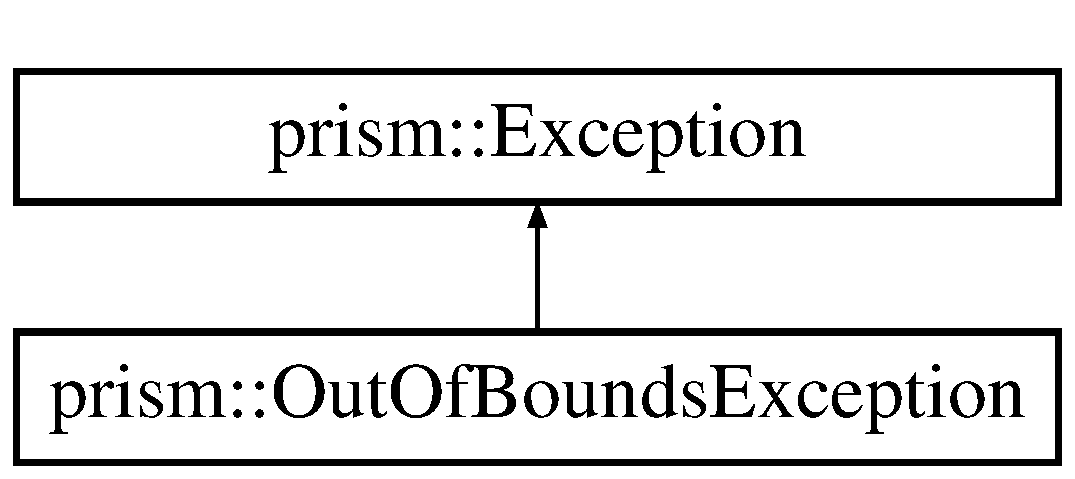
\includegraphics[height=1.996435cm]{classprism_1_1_exception}
\end{center}
\end{figure}
\subsection*{Public Member Functions}
\begin{DoxyCompactItemize}
\item 
\hyperlink{classprism_1_1_exception_ae878686fee2f57a9461a306a6a1e0fe7}{Exception} (const std\+::string \&\hyperlink{classprism_1_1_exception_ab768e96bc8a3f617b3420e19a18caf9f}{msg})
\item 
const std\+::string \& \hyperlink{classprism_1_1_exception_aba1bf849ad38dd259361be85672fc309}{error\+Msg} () const 
\end{DoxyCompactItemize}
\subsection*{Protected Member Functions}
\begin{DoxyCompactItemize}
\item 
\hyperlink{classprism_1_1_exception_aa99b00004a3c6643adbcf7c7575fd0ce}{Exception} ()
\end{DoxyCompactItemize}
\subsection*{Protected Attributes}
\begin{DoxyCompactItemize}
\item 
std\+::string \hyperlink{classprism_1_1_exception_ab768e96bc8a3f617b3420e19a18caf9f}{msg}
\end{DoxyCompactItemize}


\subsection{Constructor \& Destructor Documentation}
\index{prism\+::\+Exception@{prism\+::\+Exception}!Exception@{Exception}}
\index{Exception@{Exception}!prism\+::\+Exception@{prism\+::\+Exception}}
\subsubsection[{\texorpdfstring{Exception()}{Exception()}}]{\setlength{\rightskip}{0pt plus 5cm}prism\+::\+Exception\+::\+Exception (
\begin{DoxyParamCaption}
{}
\end{DoxyParamCaption}
)\hspace{0.3cm}{\ttfamily [inline]}, {\ttfamily [protected]}}\hypertarget{classprism_1_1_exception_aa99b00004a3c6643adbcf7c7575fd0ce}{}\label{classprism_1_1_exception_aa99b00004a3c6643adbcf7c7575fd0ce}
\index{prism\+::\+Exception@{prism\+::\+Exception}!Exception@{Exception}}
\index{Exception@{Exception}!prism\+::\+Exception@{prism\+::\+Exception}}
\subsubsection[{\texorpdfstring{Exception(const std\+::string \&msg)}{Exception(const std::string &msg)}}]{\setlength{\rightskip}{0pt plus 5cm}prism\+::\+Exception\+::\+Exception (
\begin{DoxyParamCaption}
\item[{const std\+::string \&}]{msg}
\end{DoxyParamCaption}
)\hspace{0.3cm}{\ttfamily [inline]}}\hypertarget{classprism_1_1_exception_ae878686fee2f57a9461a306a6a1e0fe7}{}\label{classprism_1_1_exception_ae878686fee2f57a9461a306a6a1e0fe7}


\subsection{Member Function Documentation}
\index{prism\+::\+Exception@{prism\+::\+Exception}!error\+Msg@{error\+Msg}}
\index{error\+Msg@{error\+Msg}!prism\+::\+Exception@{prism\+::\+Exception}}
\subsubsection[{\texorpdfstring{error\+Msg() const }{errorMsg() const }}]{\setlength{\rightskip}{0pt plus 5cm}const std\+::string\& prism\+::\+Exception\+::error\+Msg (
\begin{DoxyParamCaption}
{}
\end{DoxyParamCaption}
) const\hspace{0.3cm}{\ttfamily [inline]}}\hypertarget{classprism_1_1_exception_aba1bf849ad38dd259361be85672fc309}{}\label{classprism_1_1_exception_aba1bf849ad38dd259361be85672fc309}


\subsection{Member Data Documentation}
\index{prism\+::\+Exception@{prism\+::\+Exception}!msg@{msg}}
\index{msg@{msg}!prism\+::\+Exception@{prism\+::\+Exception}}
\subsubsection[{\texorpdfstring{msg}{msg}}]{\setlength{\rightskip}{0pt plus 5cm}std\+::string prism\+::\+Exception\+::msg\hspace{0.3cm}{\ttfamily [protected]}}\hypertarget{classprism_1_1_exception_ab768e96bc8a3f617b3420e19a18caf9f}{}\label{classprism_1_1_exception_ab768e96bc8a3f617b3420e19a18caf9f}


The documentation for this class was generated from the following file\+:\begin{DoxyCompactItemize}
\item 
inc/prism/\hyperlink{_exception_8h}{Exception.\+h}\end{DoxyCompactItemize}

\hypertarget{classprism_1_1_flag}{}\section{prism\+:\+:Flag Class Reference}
\label{classprism_1_1_flag}\index{prism\+::\+Flag@{prism\+::\+Flag}}
\subsection*{Public Member Functions}
\begin{DoxyCompactItemize}
\item 
\hyperlink{classprism_1_1_flag_aa1d5c600767c5827d5b019c73316f8c5}{Flag} (int i)
\item 
\hyperlink{classprism_1_1_flag_a1f87dfe6acac009fed137b0faa23c31f}{operator int} () const 
\end{DoxyCompactItemize}


\subsection{Constructor \& Destructor Documentation}
\index{prism\+::\+Flag@{prism\+::\+Flag}!Flag@{Flag}}
\index{Flag@{Flag}!prism\+::\+Flag@{prism\+::\+Flag}}
\subsubsection[{\texorpdfstring{Flag(int i)}{Flag(int i)}}]{\setlength{\rightskip}{0pt plus 5cm}prism\+::\+Flag\+::\+Flag (
\begin{DoxyParamCaption}
\item[{int}]{i}
\end{DoxyParamCaption}
)\hspace{0.3cm}{\ttfamily [inline]}}\hypertarget{classprism_1_1_flag_aa1d5c600767c5827d5b019c73316f8c5}{}\label{classprism_1_1_flag_aa1d5c600767c5827d5b019c73316f8c5}


\subsection{Member Function Documentation}
\index{prism\+::\+Flag@{prism\+::\+Flag}!operator int@{operator int}}
\index{operator int@{operator int}!prism\+::\+Flag@{prism\+::\+Flag}}
\subsubsection[{\texorpdfstring{operator int() const }{operator int() const }}]{\setlength{\rightskip}{0pt plus 5cm}prism\+::\+Flag\+::operator int (
\begin{DoxyParamCaption}
{}
\end{DoxyParamCaption}
) const\hspace{0.3cm}{\ttfamily [inline]}}\hypertarget{classprism_1_1_flag_a1f87dfe6acac009fed137b0faa23c31f}{}\label{classprism_1_1_flag_a1f87dfe6acac009fed137b0faa23c31f}


The documentation for this class was generated from the following file\+:\begin{DoxyCompactItemize}
\item 
\hyperlink{_flags_8h}{Flags.\+h}\end{DoxyCompactItemize}

\hypertarget{classprism_1_1_flags}{}\section{prism\+:\+:Flags$<$ Enum $>$ Class Template Reference}
\label{classprism_1_1_flags}\index{prism\+::\+Flags$<$ Enum $>$@{prism\+::\+Flags$<$ Enum $>$}}


{\ttfamily \#include $<$Flags.\+h$>$}

\subsection*{Public Types}
\begin{DoxyCompactItemize}
\item 
typedef Enum \hyperlink{classprism_1_1_flags_a2415ba62bc10f8590955edcb9c738e5b}{enum\+\_\+type}
\end{DoxyCompactItemize}
\subsection*{Public Member Functions}
\begin{DoxyCompactItemize}
\item 
\hyperlink{classprism_1_1_flags_ab702770c2483a4faaa20e5cb53a0cc1d}{Flags} (const \hyperlink{classprism_1_1_flags}{Flags} \&f)
\item 
\hyperlink{classprism_1_1_flags_acb2acd31ec112f36935e83f6b30fb2a2}{Flags} (Enum f)
\item 
\hyperlink{classprism_1_1_flags_a4a4b320bab3416ec612e3d7fb8d5bc9f}{Flags} (Zero=0)
\item 
\hyperlink{classprism_1_1_flags_ad84d23a80b3d05f919c5173716aee953}{Flags} (\hyperlink{classprism_1_1_flag}{Flag} f)
\item 
\hyperlink{classprism_1_1_flags}{Flags} \& \hyperlink{classprism_1_1_flags_a417a716b1fe682f70a5f9d892f9f52ae}{operator=} (const \hyperlink{classprism_1_1_flags}{Flags} \&f)
\item 
\hyperlink{classprism_1_1_flags}{Flags} \& \hyperlink{classprism_1_1_flags_a0dce2c8d69f4070adb183fd4ecd32c72}{operator\&=} (int mask)
\item 
\hyperlink{classprism_1_1_flags}{Flags} \& \hyperlink{classprism_1_1_flags_a10e8d99b32cd66730fdf5c925df8d835}{operator\&=} (unsigned int mask)
\item 
\hyperlink{classprism_1_1_flags}{Flags} \& \hyperlink{classprism_1_1_flags_ae45501369741bec949c438e33abaa691}{operator$\vert$=} (\hyperlink{classprism_1_1_flags}{Flags} f)
\item 
\hyperlink{classprism_1_1_flags}{Flags} \& \hyperlink{classprism_1_1_flags_ac154dae287ae3200a19ccdd4236750ad}{operator$\vert$=} (Enum f)
\item 
\hyperlink{classprism_1_1_flags}{Flags} \& \hyperlink{classprism_1_1_flags_adbd2fc9df07db796dfe16e9cf1476110}{operator$^\wedge$=} (\hyperlink{classprism_1_1_flags}{Flags} f)
\item 
\hyperlink{classprism_1_1_flags}{Flags} \& \hyperlink{classprism_1_1_flags_ac5ace902a279edd8e5be31e4668f853a}{operator$^\wedge$=} (Enum f)
\item 
\hyperlink{classprism_1_1_flags_ad914643c0ea6304a14e738970946b146}{operator int} () const 
\item 
\hyperlink{classprism_1_1_flags}{Flags} \hyperlink{classprism_1_1_flags_a69ec60ebffd8888278650c1eb6def089}{operator$\vert$} (\hyperlink{classprism_1_1_flags}{Flags} f) const 
\item 
\hyperlink{classprism_1_1_flags}{Flags} \hyperlink{classprism_1_1_flags_a1fbd3c6ffce171e8ed6ec1dab4691c71}{operator$\vert$} (Enum f) const 
\item 
\hyperlink{classprism_1_1_flags}{Flags} \hyperlink{classprism_1_1_flags_a63842ee8385e25893f0371387fbaae79}{operator$^\wedge$} (\hyperlink{classprism_1_1_flags}{Flags} f) const 
\item 
\hyperlink{classprism_1_1_flags}{Flags} \hyperlink{classprism_1_1_flags_a558ac268c605264e2379f022bab918f3}{operator$^\wedge$} (Enum f) const 
\item 
\hyperlink{classprism_1_1_flags}{Flags} \hyperlink{classprism_1_1_flags_a3db41a3026096495b17362cd78a84321}{operator\&} (int mask) const 
\item 
\hyperlink{classprism_1_1_flags}{Flags} \hyperlink{classprism_1_1_flags_ad1b35e1f4b8a12280fd44dda7ecf1106}{operator\&} (unsigned int mask) const 
\item 
\hyperlink{classprism_1_1_flags}{Flags} \hyperlink{classprism_1_1_flags_ab00e2ffaa70a3a679cd85d796eabbcec}{operator\&} (Enum f) const 
\item 
\hyperlink{classprism_1_1_flags}{Flags} \hyperlink{classprism_1_1_flags_a758fe3b9fe01e30804061f113eccd5fc}{operator$\sim$} () const 
\item 
bool \hyperlink{classprism_1_1_flags_a26c98a1f975fe23771992e9c6ad190e7}{operator!} () const 
\item 
bool \hyperlink{classprism_1_1_flags_af7ea559d83cf7a5374a08747311d9efe}{test\+Flag} (Enum f) const 
\end{DoxyCompactItemize}


\subsection{Member Typedef Documentation}
\index{prism\+::\+Flags@{prism\+::\+Flags}!enum\+\_\+type@{enum\+\_\+type}}
\index{enum\+\_\+type@{enum\+\_\+type}!prism\+::\+Flags@{prism\+::\+Flags}}
\subsubsection[{\texorpdfstring{enum\+\_\+type}{enum_type}}]{\setlength{\rightskip}{0pt plus 5cm}template$<$typename Enum$>$ typedef Enum {\bf prism\+::\+Flags}$<$ Enum $>$\+::{\bf enum\+\_\+type}}\hypertarget{classprism_1_1_flags_a2415ba62bc10f8590955edcb9c738e5b}{}\label{classprism_1_1_flags_a2415ba62bc10f8590955edcb9c738e5b}


\subsection{Constructor \& Destructor Documentation}
\index{prism\+::\+Flags@{prism\+::\+Flags}!Flags@{Flags}}
\index{Flags@{Flags}!prism\+::\+Flags@{prism\+::\+Flags}}
\subsubsection[{\texorpdfstring{Flags(const Flags \&f)}{Flags(const Flags &f)}}]{\setlength{\rightskip}{0pt plus 5cm}template$<$typename Enum$>$ {\bf prism\+::\+Flags}$<$ Enum $>$\+::{\bf Flags} (
\begin{DoxyParamCaption}
\item[{const {\bf Flags}$<$ Enum $>$ \&}]{f}
\end{DoxyParamCaption}
)\hspace{0.3cm}{\ttfamily [inline]}}\hypertarget{classprism_1_1_flags_ab702770c2483a4faaa20e5cb53a0cc1d}{}\label{classprism_1_1_flags_ab702770c2483a4faaa20e5cb53a0cc1d}
\index{prism\+::\+Flags@{prism\+::\+Flags}!Flags@{Flags}}
\index{Flags@{Flags}!prism\+::\+Flags@{prism\+::\+Flags}}
\subsubsection[{\texorpdfstring{Flags(\+Enum f)}{Flags(Enum f)}}]{\setlength{\rightskip}{0pt plus 5cm}template$<$typename Enum$>$ {\bf prism\+::\+Flags}$<$ Enum $>$\+::{\bf Flags} (
\begin{DoxyParamCaption}
\item[{Enum}]{f}
\end{DoxyParamCaption}
)\hspace{0.3cm}{\ttfamily [inline]}}\hypertarget{classprism_1_1_flags_acb2acd31ec112f36935e83f6b30fb2a2}{}\label{classprism_1_1_flags_acb2acd31ec112f36935e83f6b30fb2a2}
\index{prism\+::\+Flags@{prism\+::\+Flags}!Flags@{Flags}}
\index{Flags@{Flags}!prism\+::\+Flags@{prism\+::\+Flags}}
\subsubsection[{\texorpdfstring{Flags(\+Zero=0)}{Flags(Zero=0)}}]{\setlength{\rightskip}{0pt plus 5cm}template$<$typename Enum$>$ {\bf prism\+::\+Flags}$<$ Enum $>$\+::{\bf Flags} (
\begin{DoxyParamCaption}
\item[{Zero}]{ = {\ttfamily 0}}
\end{DoxyParamCaption}
)\hspace{0.3cm}{\ttfamily [inline]}}\hypertarget{classprism_1_1_flags_a4a4b320bab3416ec612e3d7fb8d5bc9f}{}\label{classprism_1_1_flags_a4a4b320bab3416ec612e3d7fb8d5bc9f}
\index{prism\+::\+Flags@{prism\+::\+Flags}!Flags@{Flags}}
\index{Flags@{Flags}!prism\+::\+Flags@{prism\+::\+Flags}}
\subsubsection[{\texorpdfstring{Flags(\+Flag f)}{Flags(Flag f)}}]{\setlength{\rightskip}{0pt plus 5cm}template$<$typename Enum$>$ {\bf prism\+::\+Flags}$<$ Enum $>$\+::{\bf Flags} (
\begin{DoxyParamCaption}
\item[{{\bf Flag}}]{f}
\end{DoxyParamCaption}
)\hspace{0.3cm}{\ttfamily [inline]}}\hypertarget{classprism_1_1_flags_ad84d23a80b3d05f919c5173716aee953}{}\label{classprism_1_1_flags_ad84d23a80b3d05f919c5173716aee953}


\subsection{Member Function Documentation}
\index{prism\+::\+Flags@{prism\+::\+Flags}!operator int@{operator int}}
\index{operator int@{operator int}!prism\+::\+Flags@{prism\+::\+Flags}}
\subsubsection[{\texorpdfstring{operator int() const }{operator int() const }}]{\setlength{\rightskip}{0pt plus 5cm}template$<$typename Enum$>$ {\bf prism\+::\+Flags}$<$ Enum $>$\+::operator int (
\begin{DoxyParamCaption}
{}
\end{DoxyParamCaption}
) const\hspace{0.3cm}{\ttfamily [inline]}}\hypertarget{classprism_1_1_flags_ad914643c0ea6304a14e738970946b146}{}\label{classprism_1_1_flags_ad914643c0ea6304a14e738970946b146}
\index{prism\+::\+Flags@{prism\+::\+Flags}!operator"!@{operator"!}}
\index{operator"!@{operator"!}!prism\+::\+Flags@{prism\+::\+Flags}}
\subsubsection[{\texorpdfstring{operator"!() const }{operator!() const }}]{\setlength{\rightskip}{0pt plus 5cm}template$<$typename Enum$>$ bool {\bf prism\+::\+Flags}$<$ Enum $>$\+::operator! (
\begin{DoxyParamCaption}
{}
\end{DoxyParamCaption}
) const\hspace{0.3cm}{\ttfamily [inline]}}\hypertarget{classprism_1_1_flags_a26c98a1f975fe23771992e9c6ad190e7}{}\label{classprism_1_1_flags_a26c98a1f975fe23771992e9c6ad190e7}
\index{prism\+::\+Flags@{prism\+::\+Flags}!operator\&@{operator\&}}
\index{operator\&@{operator\&}!prism\+::\+Flags@{prism\+::\+Flags}}
\subsubsection[{\texorpdfstring{operator\&(int mask) const }{operator&(int mask) const }}]{\setlength{\rightskip}{0pt plus 5cm}template$<$typename Enum$>$ {\bf Flags} {\bf prism\+::\+Flags}$<$ Enum $>$\+::operator\& (
\begin{DoxyParamCaption}
\item[{int}]{mask}
\end{DoxyParamCaption}
) const\hspace{0.3cm}{\ttfamily [inline]}}\hypertarget{classprism_1_1_flags_a3db41a3026096495b17362cd78a84321}{}\label{classprism_1_1_flags_a3db41a3026096495b17362cd78a84321}
\index{prism\+::\+Flags@{prism\+::\+Flags}!operator\&@{operator\&}}
\index{operator\&@{operator\&}!prism\+::\+Flags@{prism\+::\+Flags}}
\subsubsection[{\texorpdfstring{operator\&(unsigned int mask) const }{operator&(unsigned int mask) const }}]{\setlength{\rightskip}{0pt plus 5cm}template$<$typename Enum$>$ {\bf Flags} {\bf prism\+::\+Flags}$<$ Enum $>$\+::operator\& (
\begin{DoxyParamCaption}
\item[{unsigned int}]{mask}
\end{DoxyParamCaption}
) const\hspace{0.3cm}{\ttfamily [inline]}}\hypertarget{classprism_1_1_flags_ad1b35e1f4b8a12280fd44dda7ecf1106}{}\label{classprism_1_1_flags_ad1b35e1f4b8a12280fd44dda7ecf1106}
\index{prism\+::\+Flags@{prism\+::\+Flags}!operator\&@{operator\&}}
\index{operator\&@{operator\&}!prism\+::\+Flags@{prism\+::\+Flags}}
\subsubsection[{\texorpdfstring{operator\&(\+Enum f) const }{operator&(Enum f) const }}]{\setlength{\rightskip}{0pt plus 5cm}template$<$typename Enum$>$ {\bf Flags} {\bf prism\+::\+Flags}$<$ Enum $>$\+::operator\& (
\begin{DoxyParamCaption}
\item[{Enum}]{f}
\end{DoxyParamCaption}
) const\hspace{0.3cm}{\ttfamily [inline]}}\hypertarget{classprism_1_1_flags_ab00e2ffaa70a3a679cd85d796eabbcec}{}\label{classprism_1_1_flags_ab00e2ffaa70a3a679cd85d796eabbcec}
\index{prism\+::\+Flags@{prism\+::\+Flags}!operator\&=@{operator\&=}}
\index{operator\&=@{operator\&=}!prism\+::\+Flags@{prism\+::\+Flags}}
\subsubsection[{\texorpdfstring{operator\&=(int mask)}{operator&=(int mask)}}]{\setlength{\rightskip}{0pt plus 5cm}template$<$typename Enum$>$ {\bf Flags}\& {\bf prism\+::\+Flags}$<$ Enum $>$\+::operator\&= (
\begin{DoxyParamCaption}
\item[{int}]{mask}
\end{DoxyParamCaption}
)\hspace{0.3cm}{\ttfamily [inline]}}\hypertarget{classprism_1_1_flags_a0dce2c8d69f4070adb183fd4ecd32c72}{}\label{classprism_1_1_flags_a0dce2c8d69f4070adb183fd4ecd32c72}
\index{prism\+::\+Flags@{prism\+::\+Flags}!operator\&=@{operator\&=}}
\index{operator\&=@{operator\&=}!prism\+::\+Flags@{prism\+::\+Flags}}
\subsubsection[{\texorpdfstring{operator\&=(unsigned int mask)}{operator&=(unsigned int mask)}}]{\setlength{\rightskip}{0pt plus 5cm}template$<$typename Enum$>$ {\bf Flags}\& {\bf prism\+::\+Flags}$<$ Enum $>$\+::operator\&= (
\begin{DoxyParamCaption}
\item[{unsigned int}]{mask}
\end{DoxyParamCaption}
)\hspace{0.3cm}{\ttfamily [inline]}}\hypertarget{classprism_1_1_flags_a10e8d99b32cd66730fdf5c925df8d835}{}\label{classprism_1_1_flags_a10e8d99b32cd66730fdf5c925df8d835}
\index{prism\+::\+Flags@{prism\+::\+Flags}!operator=@{operator=}}
\index{operator=@{operator=}!prism\+::\+Flags@{prism\+::\+Flags}}
\subsubsection[{\texorpdfstring{operator=(const Flags \&f)}{operator=(const Flags &f)}}]{\setlength{\rightskip}{0pt plus 5cm}template$<$typename Enum$>$ {\bf Flags}\& {\bf prism\+::\+Flags}$<$ Enum $>$\+::operator= (
\begin{DoxyParamCaption}
\item[{const {\bf Flags}$<$ Enum $>$ \&}]{f}
\end{DoxyParamCaption}
)\hspace{0.3cm}{\ttfamily [inline]}}\hypertarget{classprism_1_1_flags_a417a716b1fe682f70a5f9d892f9f52ae}{}\label{classprism_1_1_flags_a417a716b1fe682f70a5f9d892f9f52ae}
\index{prism\+::\+Flags@{prism\+::\+Flags}!operator$^\wedge$@{operator$^\wedge$}}
\index{operator$^\wedge$@{operator$^\wedge$}!prism\+::\+Flags@{prism\+::\+Flags}}
\subsubsection[{\texorpdfstring{operator$^\wedge$(\+Flags f) const }{operator^(Flags f) const }}]{\setlength{\rightskip}{0pt plus 5cm}template$<$typename Enum$>$ {\bf Flags} {\bf prism\+::\+Flags}$<$ Enum $>$\+::operator$^\wedge$ (
\begin{DoxyParamCaption}
\item[{{\bf Flags}$<$ Enum $>$}]{f}
\end{DoxyParamCaption}
) const\hspace{0.3cm}{\ttfamily [inline]}}\hypertarget{classprism_1_1_flags_a63842ee8385e25893f0371387fbaae79}{}\label{classprism_1_1_flags_a63842ee8385e25893f0371387fbaae79}
\index{prism\+::\+Flags@{prism\+::\+Flags}!operator$^\wedge$@{operator$^\wedge$}}
\index{operator$^\wedge$@{operator$^\wedge$}!prism\+::\+Flags@{prism\+::\+Flags}}
\subsubsection[{\texorpdfstring{operator$^\wedge$(\+Enum f) const }{operator^(Enum f) const }}]{\setlength{\rightskip}{0pt plus 5cm}template$<$typename Enum$>$ {\bf Flags} {\bf prism\+::\+Flags}$<$ Enum $>$\+::operator$^\wedge$ (
\begin{DoxyParamCaption}
\item[{Enum}]{f}
\end{DoxyParamCaption}
) const\hspace{0.3cm}{\ttfamily [inline]}}\hypertarget{classprism_1_1_flags_a558ac268c605264e2379f022bab918f3}{}\label{classprism_1_1_flags_a558ac268c605264e2379f022bab918f3}
\index{prism\+::\+Flags@{prism\+::\+Flags}!operator$^\wedge$=@{operator$^\wedge$=}}
\index{operator$^\wedge$=@{operator$^\wedge$=}!prism\+::\+Flags@{prism\+::\+Flags}}
\subsubsection[{\texorpdfstring{operator$^\wedge$=(\+Flags f)}{operator^=(Flags f)}}]{\setlength{\rightskip}{0pt plus 5cm}template$<$typename Enum$>$ {\bf Flags}\& {\bf prism\+::\+Flags}$<$ Enum $>$\+::operator$^\wedge$= (
\begin{DoxyParamCaption}
\item[{{\bf Flags}$<$ Enum $>$}]{f}
\end{DoxyParamCaption}
)\hspace{0.3cm}{\ttfamily [inline]}}\hypertarget{classprism_1_1_flags_adbd2fc9df07db796dfe16e9cf1476110}{}\label{classprism_1_1_flags_adbd2fc9df07db796dfe16e9cf1476110}
\index{prism\+::\+Flags@{prism\+::\+Flags}!operator$^\wedge$=@{operator$^\wedge$=}}
\index{operator$^\wedge$=@{operator$^\wedge$=}!prism\+::\+Flags@{prism\+::\+Flags}}
\subsubsection[{\texorpdfstring{operator$^\wedge$=(\+Enum f)}{operator^=(Enum f)}}]{\setlength{\rightskip}{0pt plus 5cm}template$<$typename Enum$>$ {\bf Flags}\& {\bf prism\+::\+Flags}$<$ Enum $>$\+::operator$^\wedge$= (
\begin{DoxyParamCaption}
\item[{Enum}]{f}
\end{DoxyParamCaption}
)\hspace{0.3cm}{\ttfamily [inline]}}\hypertarget{classprism_1_1_flags_ac5ace902a279edd8e5be31e4668f853a}{}\label{classprism_1_1_flags_ac5ace902a279edd8e5be31e4668f853a}
\index{prism\+::\+Flags@{prism\+::\+Flags}!operator\texttt{"|}@{operator\texttt{"|}}}
\index{operator\texttt{"|}@{operator\texttt{"|}}!prism\+::\+Flags@{prism\+::\+Flags}}
\subsubsection[{\texorpdfstring{operator\texttt{"|}(\+Flags f) const }{operator|(Flags f) const }}]{\setlength{\rightskip}{0pt plus 5cm}template$<$typename Enum$>$ {\bf Flags} {\bf prism\+::\+Flags}$<$ Enum $>$\+::operator$\vert$ (
\begin{DoxyParamCaption}
\item[{{\bf Flags}$<$ Enum $>$}]{f}
\end{DoxyParamCaption}
) const\hspace{0.3cm}{\ttfamily [inline]}}\hypertarget{classprism_1_1_flags_a69ec60ebffd8888278650c1eb6def089}{}\label{classprism_1_1_flags_a69ec60ebffd8888278650c1eb6def089}
\index{prism\+::\+Flags@{prism\+::\+Flags}!operator\texttt{"|}@{operator\texttt{"|}}}
\index{operator\texttt{"|}@{operator\texttt{"|}}!prism\+::\+Flags@{prism\+::\+Flags}}
\subsubsection[{\texorpdfstring{operator\texttt{"|}(\+Enum f) const }{operator|(Enum f) const }}]{\setlength{\rightskip}{0pt plus 5cm}template$<$typename Enum$>$ {\bf Flags} {\bf prism\+::\+Flags}$<$ Enum $>$\+::operator$\vert$ (
\begin{DoxyParamCaption}
\item[{Enum}]{f}
\end{DoxyParamCaption}
) const\hspace{0.3cm}{\ttfamily [inline]}}\hypertarget{classprism_1_1_flags_a1fbd3c6ffce171e8ed6ec1dab4691c71}{}\label{classprism_1_1_flags_a1fbd3c6ffce171e8ed6ec1dab4691c71}
\index{prism\+::\+Flags@{prism\+::\+Flags}!operator\texttt{"|}=@{operator\texttt{"|}=}}
\index{operator\texttt{"|}=@{operator\texttt{"|}=}!prism\+::\+Flags@{prism\+::\+Flags}}
\subsubsection[{\texorpdfstring{operator\texttt{"|}=(\+Flags f)}{operator|=(Flags f)}}]{\setlength{\rightskip}{0pt plus 5cm}template$<$typename Enum$>$ {\bf Flags}\& {\bf prism\+::\+Flags}$<$ Enum $>$\+::operator$\vert$= (
\begin{DoxyParamCaption}
\item[{{\bf Flags}$<$ Enum $>$}]{f}
\end{DoxyParamCaption}
)\hspace{0.3cm}{\ttfamily [inline]}}\hypertarget{classprism_1_1_flags_ae45501369741bec949c438e33abaa691}{}\label{classprism_1_1_flags_ae45501369741bec949c438e33abaa691}
\index{prism\+::\+Flags@{prism\+::\+Flags}!operator\texttt{"|}=@{operator\texttt{"|}=}}
\index{operator\texttt{"|}=@{operator\texttt{"|}=}!prism\+::\+Flags@{prism\+::\+Flags}}
\subsubsection[{\texorpdfstring{operator\texttt{"|}=(\+Enum f)}{operator|=(Enum f)}}]{\setlength{\rightskip}{0pt plus 5cm}template$<$typename Enum$>$ {\bf Flags}\& {\bf prism\+::\+Flags}$<$ Enum $>$\+::operator$\vert$= (
\begin{DoxyParamCaption}
\item[{Enum}]{f}
\end{DoxyParamCaption}
)\hspace{0.3cm}{\ttfamily [inline]}}\hypertarget{classprism_1_1_flags_ac154dae287ae3200a19ccdd4236750ad}{}\label{classprism_1_1_flags_ac154dae287ae3200a19ccdd4236750ad}
\index{prism\+::\+Flags@{prism\+::\+Flags}!operator````~@{operator$\sim$}}
\index{operator````~@{operator$\sim$}!prism\+::\+Flags@{prism\+::\+Flags}}
\subsubsection[{\texorpdfstring{operator$\sim$() const }{operator~() const }}]{\setlength{\rightskip}{0pt plus 5cm}template$<$typename Enum$>$ {\bf Flags} {\bf prism\+::\+Flags}$<$ Enum $>$\+::operator$\sim$ (
\begin{DoxyParamCaption}
{}
\end{DoxyParamCaption}
) const\hspace{0.3cm}{\ttfamily [inline]}}\hypertarget{classprism_1_1_flags_a758fe3b9fe01e30804061f113eccd5fc}{}\label{classprism_1_1_flags_a758fe3b9fe01e30804061f113eccd5fc}
\index{prism\+::\+Flags@{prism\+::\+Flags}!test\+Flag@{test\+Flag}}
\index{test\+Flag@{test\+Flag}!prism\+::\+Flags@{prism\+::\+Flags}}
\subsubsection[{\texorpdfstring{test\+Flag(\+Enum f) const }{testFlag(Enum f) const }}]{\setlength{\rightskip}{0pt plus 5cm}template$<$typename Enum$>$ bool {\bf prism\+::\+Flags}$<$ Enum $>$\+::test\+Flag (
\begin{DoxyParamCaption}
\item[{Enum}]{f}
\end{DoxyParamCaption}
) const\hspace{0.3cm}{\ttfamily [inline]}}\hypertarget{classprism_1_1_flags_af7ea559d83cf7a5374a08747311d9efe}{}\label{classprism_1_1_flags_af7ea559d83cf7a5374a08747311d9efe}


The documentation for this class was generated from the following file\+:\begin{DoxyCompactItemize}
\item 
inc/prism/h/\hyperlink{_flags_8h}{Flags.\+h}\end{DoxyCompactItemize}

\hypertarget{structprism_1_1forward__iterator__tag}{}\section{prism\+:\+:forward\+\_\+iterator\+\_\+tag Struct Reference}
\label{structprism_1_1forward__iterator__tag}\index{prism\+::forward\+\_\+iterator\+\_\+tag@{prism\+::forward\+\_\+iterator\+\_\+tag}}
Inheritance diagram for prism\+:\+:forward\+\_\+iterator\+\_\+tag\+:\begin{figure}[H]
\begin{center}
\leavevmode
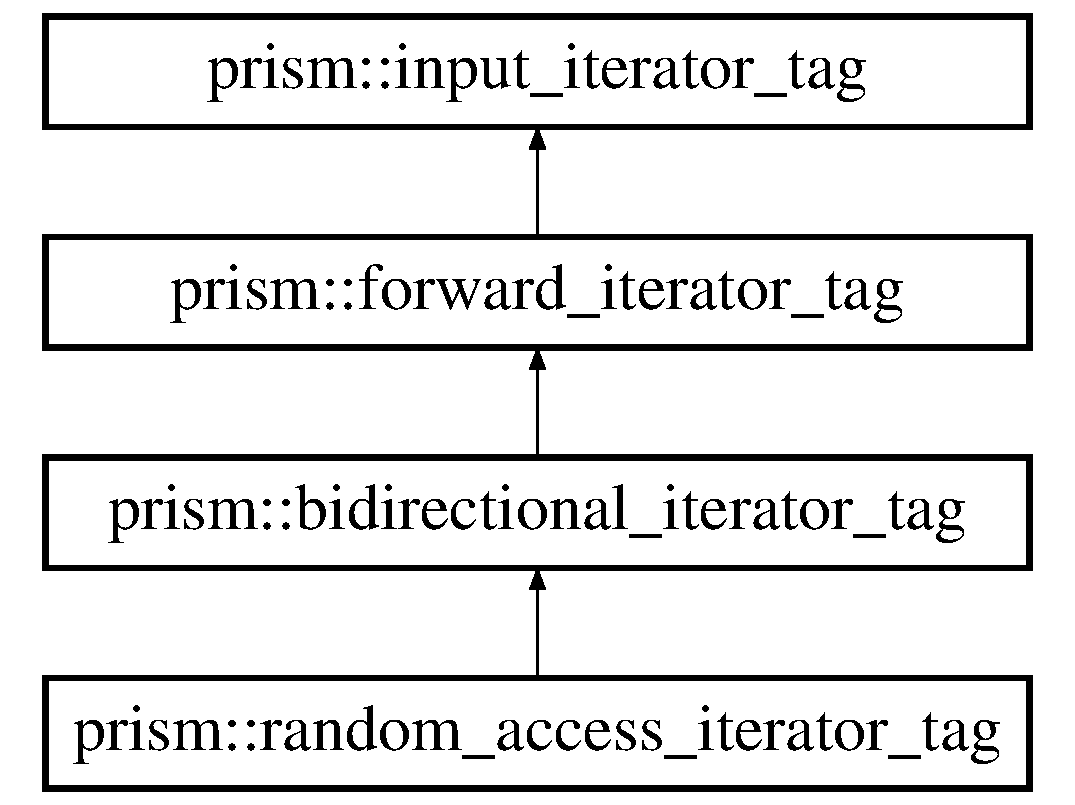
\includegraphics[height=4.000000cm]{structprism_1_1forward__iterator__tag}
\end{center}
\end{figure}


The documentation for this struct was generated from the following file\+:\begin{DoxyCompactItemize}
\item 
\hyperlink{iterator__tags_8h}{iterator\+\_\+tags.\+h}\end{DoxyCompactItemize}

\hypertarget{classprism_1_1_fraction}{}\section{prism\+:\+:Fraction Class Reference}
\label{classprism_1_1_fraction}\index{prism\+::\+Fraction@{prism\+::\+Fraction}}


{\ttfamily \#include $<$Fraction.\+h$>$}

\subsection*{Public Member Functions}
\begin{DoxyCompactItemize}
\item 
\hyperlink{classprism_1_1_fraction_ae66446d8d2130582811d17e547dd25e4}{Fraction} (void)
\item 
\hyperlink{classprism_1_1_fraction_ae6458e0578c2ddd59ce718b7808ca0ec}{Fraction} (const int \hyperlink{classprism_1_1_fraction_a1991d357549c20236a7e3008ddcc10a7}{numerator}, const int \hyperlink{classprism_1_1_fraction_af0f39f599394258c248f375c88e9c9d4}{denominator})
\item 
virtual \hyperlink{classprism_1_1_fraction_a1a7170988796417122c670c2139dc933}{$\sim$\+Fraction} (void)
\item 
const int \hyperlink{classprism_1_1_fraction_af0f39f599394258c248f375c88e9c9d4}{denominator} () const 
\item 
const int \hyperlink{classprism_1_1_fraction_a1991d357549c20236a7e3008ddcc10a7}{numerator} () const 
\item 
\hyperlink{classprism_1_1_fraction}{Fraction} \hyperlink{classprism_1_1_fraction_aab12f13967ca16e8956618f9d0641c31}{reciprocal} () const 
\item 
void \hyperlink{classprism_1_1_fraction_aeaa287cd1b228f2038b13e2bd54d5c96}{set\+Numerator} (const int \hyperlink{classprism_1_1_fraction_a1991d357549c20236a7e3008ddcc10a7}{numerator})
\item 
void \hyperlink{classprism_1_1_fraction_ac4ab0a9b891910381813f16ebc0261fa}{set\+Denominator} (const int \hyperlink{classprism_1_1_fraction_af0f39f599394258c248f375c88e9c9d4}{denominator})
\item 
\hyperlink{classprism_1_1_fraction}{Fraction} \& \hyperlink{classprism_1_1_fraction_ab30164e43aa9ce13ad3dc364b8711473}{simplify} ()
\end{DoxyCompactItemize}
\subsection*{Friends}
\begin{DoxyCompactItemize}
\item 
\hyperlink{classprism_1_1_fraction}{Fraction} \hyperlink{classprism_1_1_fraction_a225c4aec1a9cdd366b04be2642ecf3bc}{operator+} (const \hyperlink{classprism_1_1_fraction}{Fraction} \&f1, const \hyperlink{classprism_1_1_fraction}{Fraction} \&f2)
\item 
\hyperlink{classprism_1_1_fraction}{Fraction} \hyperlink{classprism_1_1_fraction_aa93e0ab89fa477f3b044cf5826df7c14}{operator-\/} (const \hyperlink{classprism_1_1_fraction}{Fraction} \&f1, const \hyperlink{classprism_1_1_fraction}{Fraction} \&f2)
\item 
\hyperlink{classprism_1_1_fraction}{Fraction} \hyperlink{classprism_1_1_fraction_ad106ee756801021779f14e992439db4a}{operator$\ast$} (const \hyperlink{classprism_1_1_fraction}{Fraction} \&f1, const \hyperlink{classprism_1_1_fraction}{Fraction} \&f2)
\item 
\hyperlink{classprism_1_1_fraction}{Fraction} \hyperlink{classprism_1_1_fraction_a00eb461e6959195ce533d9d8f9b0855d}{operator$\ast$} (const \hyperlink{classprism_1_1_fraction}{Fraction} \&fraction, const int i)
\item 
\hyperlink{classprism_1_1_fraction}{Fraction} \hyperlink{classprism_1_1_fraction_a2f76d38f8274375542a97c3154af16eb}{operator$\ast$} (const int i, const \hyperlink{classprism_1_1_fraction}{Fraction} \&fraction)
\item 
\hyperlink{classprism_1_1_fraction}{Fraction} \hyperlink{classprism_1_1_fraction_a2a185031bd64d6b227509aeacf3b5c69}{operator/} (const \hyperlink{classprism_1_1_fraction}{Fraction} \&f1, const \hyperlink{classprism_1_1_fraction}{Fraction} \&f2)
\item 
const bool \hyperlink{classprism_1_1_fraction_a557b4641e321113411fe440a2bc4e9cb}{operator$<$} (const \hyperlink{classprism_1_1_fraction}{Fraction} \&f1, const \hyperlink{classprism_1_1_fraction}{Fraction} \&f2)
\item 
const bool \hyperlink{classprism_1_1_fraction_a4307a97fd1a744418e8e2d64fb05ffd5}{operator$>$} (const \hyperlink{classprism_1_1_fraction}{Fraction} \&f1, const \hyperlink{classprism_1_1_fraction}{Fraction} \&f2)
\item 
const bool \hyperlink{classprism_1_1_fraction_a061d9325f891c3601d892edce079652b}{operator==} (const \hyperlink{classprism_1_1_fraction}{Fraction} \&f1, const \hyperlink{classprism_1_1_fraction}{Fraction} \&f2)
\item 
const bool \hyperlink{classprism_1_1_fraction_a2469410854b8425a70b1489afa5651d5}{operator!=} (const \hyperlink{classprism_1_1_fraction}{Fraction} \&f1, const \hyperlink{classprism_1_1_fraction}{Fraction} \&f2)
\item 
std\+::ostream \& \hyperlink{classprism_1_1_fraction_aae68a18403f22736f297b8671746f144}{operator$<$$<$} (std\+::ostream \&out, const \hyperlink{classprism_1_1_fraction}{Fraction} \&f)
\end{DoxyCompactItemize}


\subsection{Constructor \& Destructor Documentation}
\index{prism\+::\+Fraction@{prism\+::\+Fraction}!Fraction@{Fraction}}
\index{Fraction@{Fraction}!prism\+::\+Fraction@{prism\+::\+Fraction}}
\subsubsection[{\texorpdfstring{Fraction(void)}{Fraction(void)}}]{\setlength{\rightskip}{0pt plus 5cm}prism\+::\+Fraction\+::\+Fraction (
\begin{DoxyParamCaption}
\item[{void}]{}
\end{DoxyParamCaption}
)}\hypertarget{classprism_1_1_fraction_ae66446d8d2130582811d17e547dd25e4}{}\label{classprism_1_1_fraction_ae66446d8d2130582811d17e547dd25e4}
Creates a \hyperlink{classprism_1_1_fraction}{Fraction} object and sets its numerator and denominator to 1. \index{prism\+::\+Fraction@{prism\+::\+Fraction}!Fraction@{Fraction}}
\index{Fraction@{Fraction}!prism\+::\+Fraction@{prism\+::\+Fraction}}
\subsubsection[{\texorpdfstring{Fraction(const int numerator, const int denominator)}{Fraction(const int numerator, const int denominator)}}]{\setlength{\rightskip}{0pt plus 5cm}prism\+::\+Fraction\+::\+Fraction (
\begin{DoxyParamCaption}
\item[{const int}]{numerator, }
\item[{const int}]{denominator}
\end{DoxyParamCaption}
)}\hypertarget{classprism_1_1_fraction_ae6458e0578c2ddd59ce718b7808ca0ec}{}\label{classprism_1_1_fraction_ae6458e0578c2ddd59ce718b7808ca0ec}
Creates a \hyperlink{classprism_1_1_fraction}{Fraction} object setting the numerator and denominator to the values passed in. The class will attempt to simplify the fraction. i.\+e. 4 1 --- becomes --- 8 2 \index{prism\+::\+Fraction@{prism\+::\+Fraction}!````~Fraction@{$\sim$\+Fraction}}
\index{````~Fraction@{$\sim$\+Fraction}!prism\+::\+Fraction@{prism\+::\+Fraction}}
\subsubsection[{\texorpdfstring{$\sim$\+Fraction(void)}{~Fraction(void)}}]{\setlength{\rightskip}{0pt plus 5cm}prism\+::\+Fraction\+::$\sim$\+Fraction (
\begin{DoxyParamCaption}
\item[{void}]{}
\end{DoxyParamCaption}
)\hspace{0.3cm}{\ttfamily [virtual]}}\hypertarget{classprism_1_1_fraction_a1a7170988796417122c670c2139dc933}{}\label{classprism_1_1_fraction_a1a7170988796417122c670c2139dc933}
Destroys this \hyperlink{classprism_1_1_fraction}{Fraction}. 

\subsection{Member Function Documentation}
\index{prism\+::\+Fraction@{prism\+::\+Fraction}!denominator@{denominator}}
\index{denominator@{denominator}!prism\+::\+Fraction@{prism\+::\+Fraction}}
\subsubsection[{\texorpdfstring{denominator() const }{denominator() const }}]{\setlength{\rightskip}{0pt plus 5cm}const int prism\+::\+Fraction\+::denominator (
\begin{DoxyParamCaption}
{}
\end{DoxyParamCaption}
) const}\hypertarget{classprism_1_1_fraction_af0f39f599394258c248f375c88e9c9d4}{}\label{classprism_1_1_fraction_af0f39f599394258c248f375c88e9c9d4}
Returns this \hyperlink{classprism_1_1_fraction}{Fraction}\textquotesingle{}s denominator. \index{prism\+::\+Fraction@{prism\+::\+Fraction}!numerator@{numerator}}
\index{numerator@{numerator}!prism\+::\+Fraction@{prism\+::\+Fraction}}
\subsubsection[{\texorpdfstring{numerator() const }{numerator() const }}]{\setlength{\rightskip}{0pt plus 5cm}const int prism\+::\+Fraction\+::numerator (
\begin{DoxyParamCaption}
{}
\end{DoxyParamCaption}
) const}\hypertarget{classprism_1_1_fraction_a1991d357549c20236a7e3008ddcc10a7}{}\label{classprism_1_1_fraction_a1991d357549c20236a7e3008ddcc10a7}
Returns this \hyperlink{classprism_1_1_fraction}{Fraction}\textquotesingle{}s numerator. \index{prism\+::\+Fraction@{prism\+::\+Fraction}!reciprocal@{reciprocal}}
\index{reciprocal@{reciprocal}!prism\+::\+Fraction@{prism\+::\+Fraction}}
\subsubsection[{\texorpdfstring{reciprocal() const }{reciprocal() const }}]{\setlength{\rightskip}{0pt plus 5cm}{\bf Fraction} prism\+::\+Fraction\+::reciprocal (
\begin{DoxyParamCaption}
{}
\end{DoxyParamCaption}
) const}\hypertarget{classprism_1_1_fraction_aab12f13967ca16e8956618f9d0641c31}{}\label{classprism_1_1_fraction_aab12f13967ca16e8956618f9d0641c31}
Returns a new \hyperlink{classprism_1_1_fraction}{Fraction} that is the reciprocal of this fraction. i.\+e. the numerator and denominator are swapped around. 1 2 The reciprocal of --- is --- 2 1 Any fraction multiplied by its own reciprocal will always equal 1. \index{prism\+::\+Fraction@{prism\+::\+Fraction}!set\+Denominator@{set\+Denominator}}
\index{set\+Denominator@{set\+Denominator}!prism\+::\+Fraction@{prism\+::\+Fraction}}
\subsubsection[{\texorpdfstring{set\+Denominator(const int denominator)}{setDenominator(const int denominator)}}]{\setlength{\rightskip}{0pt plus 5cm}void prism\+::\+Fraction\+::set\+Denominator (
\begin{DoxyParamCaption}
\item[{const int}]{denominator}
\end{DoxyParamCaption}
)}\hypertarget{classprism_1_1_fraction_ac4ab0a9b891910381813f16ebc0261fa}{}\label{classprism_1_1_fraction_ac4ab0a9b891910381813f16ebc0261fa}
Sets this \hyperlink{classprism_1_1_fraction}{Fraction}\textquotesingle{}s denominator to /em denominator. \index{prism\+::\+Fraction@{prism\+::\+Fraction}!set\+Numerator@{set\+Numerator}}
\index{set\+Numerator@{set\+Numerator}!prism\+::\+Fraction@{prism\+::\+Fraction}}
\subsubsection[{\texorpdfstring{set\+Numerator(const int numerator)}{setNumerator(const int numerator)}}]{\setlength{\rightskip}{0pt plus 5cm}void prism\+::\+Fraction\+::set\+Numerator (
\begin{DoxyParamCaption}
\item[{const int}]{numerator}
\end{DoxyParamCaption}
)}\hypertarget{classprism_1_1_fraction_aeaa287cd1b228f2038b13e2bd54d5c96}{}\label{classprism_1_1_fraction_aeaa287cd1b228f2038b13e2bd54d5c96}
Sets this \hyperlink{classprism_1_1_fraction}{Fraction}\textquotesingle{}s numerator to /em numerator. \index{prism\+::\+Fraction@{prism\+::\+Fraction}!simplify@{simplify}}
\index{simplify@{simplify}!prism\+::\+Fraction@{prism\+::\+Fraction}}
\subsubsection[{\texorpdfstring{simplify()}{simplify()}}]{\setlength{\rightskip}{0pt plus 5cm}{\bf Fraction} \& prism\+::\+Fraction\+::simplify (
\begin{DoxyParamCaption}
{}
\end{DoxyParamCaption}
)}\hypertarget{classprism_1_1_fraction_ab30164e43aa9ce13ad3dc364b8711473}{}\label{classprism_1_1_fraction_ab30164e43aa9ce13ad3dc364b8711473}
\subsubsection*{8 }

16 

\subsection{Friends And Related Function Documentation}
\index{prism\+::\+Fraction@{prism\+::\+Fraction}!operator"!=@{operator"!=}}
\index{operator"!=@{operator"!=}!prism\+::\+Fraction@{prism\+::\+Fraction}}
\subsubsection[{\texorpdfstring{operator"!=}{operator!=}}]{\setlength{\rightskip}{0pt plus 5cm}const bool operator!= (
\begin{DoxyParamCaption}
\item[{const {\bf Fraction} \&}]{f1, }
\item[{const {\bf Fraction} \&}]{f2}
\end{DoxyParamCaption}
)\hspace{0.3cm}{\ttfamily [friend]}}\hypertarget{classprism_1_1_fraction_a2469410854b8425a70b1489afa5651d5}{}\label{classprism_1_1_fraction_a2469410854b8425a70b1489afa5651d5}
Returns true if /em f1 does not equal /em f2 in value, false otherwise. \index{prism\+::\+Fraction@{prism\+::\+Fraction}!operator$\ast$@{operator$\ast$}}
\index{operator$\ast$@{operator$\ast$}!prism\+::\+Fraction@{prism\+::\+Fraction}}
\subsubsection[{\texorpdfstring{operator$\ast$}{operator*}}]{\setlength{\rightskip}{0pt plus 5cm}{\bf Fraction} operator$\ast$ (
\begin{DoxyParamCaption}
\item[{const {\bf Fraction} \&}]{f1, }
\item[{const {\bf Fraction} \&}]{f2}
\end{DoxyParamCaption}
)\hspace{0.3cm}{\ttfamily [friend]}}\hypertarget{classprism_1_1_fraction_ad106ee756801021779f14e992439db4a}{}\label{classprism_1_1_fraction_ad106ee756801021779f14e992439db4a}
Multiplies /em f1 and /em f2 together and returns a new \hyperlink{classprism_1_1_fraction}{Fraction}. \hyperlink{classprism_1_1_fraction}{Fraction} multiplication is the easiest arithmetical operation. Simply multiply the two numerators together to form the new numerator and multiply the two denominators together to form the new denominator. e.\+g. 2 8 2x8 16 4 --- x --- = --- = --- = --- 5 4 5x4 20 5 \index{prism\+::\+Fraction@{prism\+::\+Fraction}!operator$\ast$@{operator$\ast$}}
\index{operator$\ast$@{operator$\ast$}!prism\+::\+Fraction@{prism\+::\+Fraction}}
\subsubsection[{\texorpdfstring{operator$\ast$}{operator*}}]{\setlength{\rightskip}{0pt plus 5cm}{\bf Fraction} operator$\ast$ (
\begin{DoxyParamCaption}
\item[{const {\bf Fraction} \&}]{fraction, }
\item[{const int}]{i}
\end{DoxyParamCaption}
)\hspace{0.3cm}{\ttfamily [friend]}}\hypertarget{classprism_1_1_fraction_a00eb461e6959195ce533d9d8f9b0855d}{}\label{classprism_1_1_fraction_a00eb461e6959195ce533d9d8f9b0855d}
Multiplies the \hyperlink{classprism_1_1_fraction}{Fraction} /em fraction by the whole number /em i. Returns a new \hyperlink{classprism_1_1_fraction}{Fraction}. \index{prism\+::\+Fraction@{prism\+::\+Fraction}!operator$\ast$@{operator$\ast$}}
\index{operator$\ast$@{operator$\ast$}!prism\+::\+Fraction@{prism\+::\+Fraction}}
\subsubsection[{\texorpdfstring{operator$\ast$}{operator*}}]{\setlength{\rightskip}{0pt plus 5cm}{\bf Fraction} operator$\ast$ (
\begin{DoxyParamCaption}
\item[{const int}]{i, }
\item[{const {\bf Fraction} \&}]{fraction}
\end{DoxyParamCaption}
)\hspace{0.3cm}{\ttfamily [friend]}}\hypertarget{classprism_1_1_fraction_a2f76d38f8274375542a97c3154af16eb}{}\label{classprism_1_1_fraction_a2f76d38f8274375542a97c3154af16eb}
Multiplies the whole number /em i by the \hyperlink{classprism_1_1_fraction}{Fraction} /em fraction. Returns a new \hyperlink{classprism_1_1_fraction}{Fraction}. \index{prism\+::\+Fraction@{prism\+::\+Fraction}!operator+@{operator+}}
\index{operator+@{operator+}!prism\+::\+Fraction@{prism\+::\+Fraction}}
\subsubsection[{\texorpdfstring{operator+}{operator+}}]{\setlength{\rightskip}{0pt plus 5cm}{\bf Fraction} operator+ (
\begin{DoxyParamCaption}
\item[{const {\bf Fraction} \&}]{f1, }
\item[{const {\bf Fraction} \&}]{f2}
\end{DoxyParamCaption}
)\hspace{0.3cm}{\ttfamily [friend]}}\hypertarget{classprism_1_1_fraction_a225c4aec1a9cdd366b04be2642ecf3bc}{}\label{classprism_1_1_fraction_a225c4aec1a9cdd366b04be2642ecf3bc}
Adds the fractions /em f1 and /em f2 together and returns a new \hyperlink{classprism_1_1_fraction}{Fraction}. If the two denominators are the same then the two numerators are added together to form the new numerator and the original denominator is kept the same. e.\+g. 1 1 2 --- + --- = --- 4 4 4 If the denominators are different then we alter the fractions in order to make both denominators the same value. We make a whole fraction out of the second fraction\textquotesingle{}s denominator and multiply it by the first fraction. Then make a whole fraction from the first fraction\textquotesingle{}s denominator and multiply it by the second fraction. Now we can simply add together the two numerators and keep the denominator the same. 1 1 $\vert$ 4 1 $\vert$ $\vert$ 1 2 $\vert$ 4 2 6 3 --- + --- = $\vert$--- x ---$\vert$ + $\vert$--- x ---$\vert$ = --- + --- = --- = --- 2 4 $\vert$ 4 2 $\vert$ $\vert$ 4 2 $\vert$ 8 8 8 4 \index{prism\+::\+Fraction@{prism\+::\+Fraction}!operator-\/@{operator-\/}}
\index{operator-\/@{operator-\/}!prism\+::\+Fraction@{prism\+::\+Fraction}}
\subsubsection[{\texorpdfstring{operator-\/}{operator-}}]{\setlength{\rightskip}{0pt plus 5cm}{\bf Fraction} operator-\/ (
\begin{DoxyParamCaption}
\item[{const {\bf Fraction} \&}]{f1, }
\item[{const {\bf Fraction} \&}]{f2}
\end{DoxyParamCaption}
)\hspace{0.3cm}{\ttfamily [friend]}}\hypertarget{classprism_1_1_fraction_aa93e0ab89fa477f3b044cf5826df7c14}{}\label{classprism_1_1_fraction_aa93e0ab89fa477f3b044cf5826df7c14}
Subtracts the fractions /em f1 and /em f2 and returns a new \hyperlink{classprism_1_1_fraction}{Fraction}. If the two denominators are the same then the two numerators are subtracted to form the new numerator and the original denominator is kept the same. e.\+g. 3 1 2 --- -\/ --- = --- 4 4 4 If the denominators are different then we alter the fractions in order to make both denominators the same value. We make a whole fraction out of the second fraction\textquotesingle{}s denominator and multiply it by the first fraction. Then make a whole fraction from the first fraction\textquotesingle{}s denominator and multiply it by the second fraction. Now we can simply subtract the two numerators and keep the denominator the same. 3 1 $\vert$ 2 3 $\vert$ $\vert$ 1 4 $\vert$ 6 4 2 1 --- -\/ --- = $\vert$--- x ---$\vert$ -\/ $\vert$--- x ---$\vert$ = --- -\/ --- = --- = --- 4 2 $\vert$ 2 4 $\vert$ $\vert$ 2 4 $\vert$ 8 8 8 4 \index{prism\+::\+Fraction@{prism\+::\+Fraction}!operator/@{operator/}}
\index{operator/@{operator/}!prism\+::\+Fraction@{prism\+::\+Fraction}}
\subsubsection[{\texorpdfstring{operator/}{operator/}}]{\setlength{\rightskip}{0pt plus 5cm}{\bf Fraction} operator/ (
\begin{DoxyParamCaption}
\item[{const {\bf Fraction} \&}]{f1, }
\item[{const {\bf Fraction} \&}]{f2}
\end{DoxyParamCaption}
)\hspace{0.3cm}{\ttfamily [friend]}}\hypertarget{classprism_1_1_fraction_a2a185031bd64d6b227509aeacf3b5c69}{}\label{classprism_1_1_fraction_a2a185031bd64d6b227509aeacf3b5c69}
Divides /em f1 by /em f2 and returns a new \hyperlink{classprism_1_1_fraction}{Fraction}. \hyperlink{classprism_1_1_fraction}{Fraction} division is achieved by taking the reciprocal of the second fraction and multiplying it against the first fraction. See /em \hyperlink{classprism_1_1_fraction_aab12f13967ca16e8956618f9d0641c31}{Fraction\+::reciprocal()} for more information. 3 2 3 7 21 --- / --- = --- $\ast$ --- = --- 4 7 4 2 8 \index{prism\+::\+Fraction@{prism\+::\+Fraction}!operator$<$@{operator$<$}}
\index{operator$<$@{operator$<$}!prism\+::\+Fraction@{prism\+::\+Fraction}}
\subsubsection[{\texorpdfstring{operator$<$}{operator<}}]{\setlength{\rightskip}{0pt plus 5cm}const bool operator$<$ (
\begin{DoxyParamCaption}
\item[{const {\bf Fraction} \&}]{f1, }
\item[{const {\bf Fraction} \&}]{f2}
\end{DoxyParamCaption}
)\hspace{0.3cm}{\ttfamily [friend]}}\hypertarget{classprism_1_1_fraction_a557b4641e321113411fe440a2bc4e9cb}{}\label{classprism_1_1_fraction_a557b4641e321113411fe440a2bc4e9cb}
Returns true if /em f1 is less than /em f2, false otherwise. \index{prism\+::\+Fraction@{prism\+::\+Fraction}!operator$<$$<$@{operator$<$$<$}}
\index{operator$<$$<$@{operator$<$$<$}!prism\+::\+Fraction@{prism\+::\+Fraction}}
\subsubsection[{\texorpdfstring{operator$<$$<$}{operator<<}}]{\setlength{\rightskip}{0pt plus 5cm}std\+::ostream\& operator$<$$<$ (
\begin{DoxyParamCaption}
\item[{std\+::ostream \&}]{out, }
\item[{const {\bf Fraction} \&}]{f}
\end{DoxyParamCaption}
)\hspace{0.3cm}{\ttfamily [friend]}}\hypertarget{classprism_1_1_fraction_aae68a18403f22736f297b8671746f144}{}\label{classprism_1_1_fraction_aae68a18403f22736f297b8671746f144}
Allows an instance of \hyperlink{classprism_1_1_fraction}{Fraction} to be written to the ostream and returns a reference to the ostream. \index{prism\+::\+Fraction@{prism\+::\+Fraction}!operator==@{operator==}}
\index{operator==@{operator==}!prism\+::\+Fraction@{prism\+::\+Fraction}}
\subsubsection[{\texorpdfstring{operator==}{operator==}}]{\setlength{\rightskip}{0pt plus 5cm}const bool operator== (
\begin{DoxyParamCaption}
\item[{const {\bf Fraction} \&}]{f1, }
\item[{const {\bf Fraction} \&}]{f2}
\end{DoxyParamCaption}
)\hspace{0.3cm}{\ttfamily [friend]}}\hypertarget{classprism_1_1_fraction_a061d9325f891c3601d892edce079652b}{}\label{classprism_1_1_fraction_a061d9325f891c3601d892edce079652b}
Returns true if /em f1 and /em f2 are equal in value. \index{prism\+::\+Fraction@{prism\+::\+Fraction}!operator$>$@{operator$>$}}
\index{operator$>$@{operator$>$}!prism\+::\+Fraction@{prism\+::\+Fraction}}
\subsubsection[{\texorpdfstring{operator$>$}{operator>}}]{\setlength{\rightskip}{0pt plus 5cm}const bool operator$>$ (
\begin{DoxyParamCaption}
\item[{const {\bf Fraction} \&}]{f1, }
\item[{const {\bf Fraction} \&}]{f2}
\end{DoxyParamCaption}
)\hspace{0.3cm}{\ttfamily [friend]}}\hypertarget{classprism_1_1_fraction_a4307a97fd1a744418e8e2d64fb05ffd5}{}\label{classprism_1_1_fraction_a4307a97fd1a744418e8e2d64fb05ffd5}
Returns true if /em f1 is less than /em f2, false otherwise. 

The documentation for this class was generated from the following files\+:\begin{DoxyCompactItemize}
\item 
inc/prism/h/\hyperlink{_fraction_8h}{Fraction.\+h}\item 
src/prism/\hyperlink{_fraction_8cpp}{Fraction.\+cpp}\end{DoxyCompactItemize}

\hypertarget{structprism_1_1greater}{}\section{prism\+:\+:greater$<$ T $>$ Struct Template Reference}
\label{structprism_1_1greater}\index{prism\+::greater$<$ T $>$@{prism\+::greater$<$ T $>$}}
\subsection*{Public Member Functions}
\begin{DoxyCompactItemize}
\item 
bool \hyperlink{structprism_1_1greater_a2c952be396da8d9585299534e8935ba0}{operator()} (const T \&a, const T \&b)
\end{DoxyCompactItemize}


\subsection{Detailed Description}
\subsubsection*{template$<$class T$>$\\*
struct prism\+::greater$<$ T $>$}

Returns true if a is greater than b, false otherwise. 

\subsection{Member Function Documentation}
\index{prism\+::greater@{prism\+::greater}!operator()@{operator()}}
\index{operator()@{operator()}!prism\+::greater@{prism\+::greater}}
\subsubsection[{\texorpdfstring{operator()(const T \&a, const T \&b)}{operator()(const T &a, const T &b)}}]{\setlength{\rightskip}{0pt plus 5cm}template$<$class T $>$ bool {\bf prism\+::greater}$<$ T $>$\+::operator() (
\begin{DoxyParamCaption}
\item[{const T \&}]{a, }
\item[{const T \&}]{b}
\end{DoxyParamCaption}
)\hspace{0.3cm}{\ttfamily [inline]}}\hypertarget{structprism_1_1greater_a2c952be396da8d9585299534e8935ba0}{}\label{structprism_1_1greater_a2c952be396da8d9585299534e8935ba0}


The documentation for this struct was generated from the following file\+:\begin{DoxyCompactItemize}
\item 
\hyperlink{functor_8h}{functor.\+h}\end{DoxyCompactItemize}

\hypertarget{structprism_1_1input__iterator__tag}{}\section{prism\+:\+:input\+\_\+iterator\+\_\+tag Struct Reference}
\label{structprism_1_1input__iterator__tag}\index{prism\+::input\+\_\+iterator\+\_\+tag@{prism\+::input\+\_\+iterator\+\_\+tag}}
Inheritance diagram for prism\+:\+:input\+\_\+iterator\+\_\+tag\+:\begin{figure}[H]
\begin{center}
\leavevmode
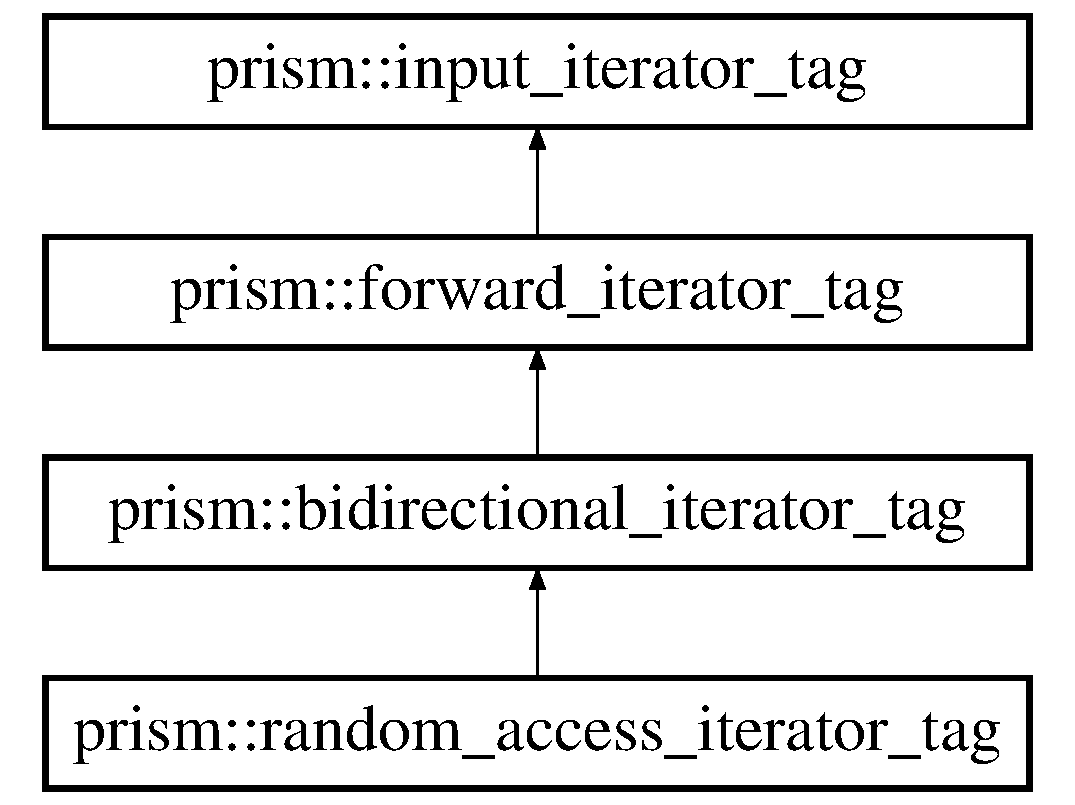
\includegraphics[height=4.000000cm]{structprism_1_1input__iterator__tag}
\end{center}
\end{figure}


The documentation for this struct was generated from the following file\+:\begin{DoxyCompactItemize}
\item 
\hyperlink{iterator_8h}{iterator.\+h}\end{DoxyCompactItemize}

\hypertarget{structprism_1_1iterator__traits}{}\section{prism\+:\+:iterator\+\_\+traits$<$ Iterator $>$ Struct Template Reference}
\label{structprism_1_1iterator__traits}\index{prism\+::iterator\+\_\+traits$<$ Iterator $>$@{prism\+::iterator\+\_\+traits$<$ Iterator $>$}}
\subsection*{Public Types}
\begin{DoxyCompactItemize}
\item 
typedef Iterator\+::value\+\_\+type \hyperlink{structprism_1_1iterator__traits_a897219622ddfbb1f94aba0cc575cb30c}{value\+\_\+type}
\item 
typedef Iterator\+::difference\+\_\+type \hyperlink{structprism_1_1iterator__traits_ae78f6fab069fd9118d558db5d4f81d54}{difference\+\_\+type}
\item 
typedef Iterator\+::iterator\+\_\+category \hyperlink{structprism_1_1iterator__traits_a3ae4da59bd72e7026c5fe2a23e799e1b}{iterator\+\_\+category}
\item 
typedef Iterator\+::pointer \hyperlink{structprism_1_1iterator__traits_a74c12fd61a29bfd2a645a8d798e93810}{pointer}
\item 
typedef Iterator\+::const\+\_\+pointer \hyperlink{structprism_1_1iterator__traits_a6acb84b2431eb855d4e51c8dd16cb5e5}{const\+\_\+pointer}
\item 
typedef Iterator\+::reference \hyperlink{structprism_1_1iterator__traits_a18c26ae6eea81bdaeb3bd4e15038eca7}{reference}
\item 
typedef Iterator\+::const\+\_\+reference \hyperlink{structprism_1_1iterator__traits_a27032f81f31f64773f63693623fd4023}{const\+\_\+reference}
\end{DoxyCompactItemize}


\subsection{Member Typedef Documentation}
\index{prism\+::iterator\+\_\+traits@{prism\+::iterator\+\_\+traits}!const\+\_\+pointer@{const\+\_\+pointer}}
\index{const\+\_\+pointer@{const\+\_\+pointer}!prism\+::iterator\+\_\+traits@{prism\+::iterator\+\_\+traits}}
\subsubsection[{\texorpdfstring{const\+\_\+pointer}{const_pointer}}]{\setlength{\rightskip}{0pt plus 5cm}template$<$class Iterator$>$ typedef Iterator\+::const\+\_\+pointer {\bf prism\+::iterator\+\_\+traits}$<$ Iterator $>$\+::{\bf const\+\_\+pointer}}\hypertarget{structprism_1_1iterator__traits_a6acb84b2431eb855d4e51c8dd16cb5e5}{}\label{structprism_1_1iterator__traits_a6acb84b2431eb855d4e51c8dd16cb5e5}
\index{prism\+::iterator\+\_\+traits@{prism\+::iterator\+\_\+traits}!const\+\_\+reference@{const\+\_\+reference}}
\index{const\+\_\+reference@{const\+\_\+reference}!prism\+::iterator\+\_\+traits@{prism\+::iterator\+\_\+traits}}
\subsubsection[{\texorpdfstring{const\+\_\+reference}{const_reference}}]{\setlength{\rightskip}{0pt plus 5cm}template$<$class Iterator$>$ typedef Iterator\+::const\+\_\+reference {\bf prism\+::iterator\+\_\+traits}$<$ Iterator $>$\+::{\bf const\+\_\+reference}}\hypertarget{structprism_1_1iterator__traits_a27032f81f31f64773f63693623fd4023}{}\label{structprism_1_1iterator__traits_a27032f81f31f64773f63693623fd4023}
\index{prism\+::iterator\+\_\+traits@{prism\+::iterator\+\_\+traits}!difference\+\_\+type@{difference\+\_\+type}}
\index{difference\+\_\+type@{difference\+\_\+type}!prism\+::iterator\+\_\+traits@{prism\+::iterator\+\_\+traits}}
\subsubsection[{\texorpdfstring{difference\+\_\+type}{difference_type}}]{\setlength{\rightskip}{0pt plus 5cm}template$<$class Iterator$>$ typedef Iterator\+::difference\+\_\+type {\bf prism\+::iterator\+\_\+traits}$<$ Iterator $>$\+::{\bf difference\+\_\+type}}\hypertarget{structprism_1_1iterator__traits_ae78f6fab069fd9118d558db5d4f81d54}{}\label{structprism_1_1iterator__traits_ae78f6fab069fd9118d558db5d4f81d54}
\index{prism\+::iterator\+\_\+traits@{prism\+::iterator\+\_\+traits}!iterator\+\_\+category@{iterator\+\_\+category}}
\index{iterator\+\_\+category@{iterator\+\_\+category}!prism\+::iterator\+\_\+traits@{prism\+::iterator\+\_\+traits}}
\subsubsection[{\texorpdfstring{iterator\+\_\+category}{iterator_category}}]{\setlength{\rightskip}{0pt plus 5cm}template$<$class Iterator$>$ typedef Iterator\+::iterator\+\_\+category {\bf prism\+::iterator\+\_\+traits}$<$ Iterator $>$\+::{\bf iterator\+\_\+category}}\hypertarget{structprism_1_1iterator__traits_a3ae4da59bd72e7026c5fe2a23e799e1b}{}\label{structprism_1_1iterator__traits_a3ae4da59bd72e7026c5fe2a23e799e1b}
\index{prism\+::iterator\+\_\+traits@{prism\+::iterator\+\_\+traits}!pointer@{pointer}}
\index{pointer@{pointer}!prism\+::iterator\+\_\+traits@{prism\+::iterator\+\_\+traits}}
\subsubsection[{\texorpdfstring{pointer}{pointer}}]{\setlength{\rightskip}{0pt plus 5cm}template$<$class Iterator$>$ typedef Iterator\+::pointer {\bf prism\+::iterator\+\_\+traits}$<$ Iterator $>$\+::{\bf pointer}}\hypertarget{structprism_1_1iterator__traits_a74c12fd61a29bfd2a645a8d798e93810}{}\label{structprism_1_1iterator__traits_a74c12fd61a29bfd2a645a8d798e93810}
\index{prism\+::iterator\+\_\+traits@{prism\+::iterator\+\_\+traits}!reference@{reference}}
\index{reference@{reference}!prism\+::iterator\+\_\+traits@{prism\+::iterator\+\_\+traits}}
\subsubsection[{\texorpdfstring{reference}{reference}}]{\setlength{\rightskip}{0pt plus 5cm}template$<$class Iterator$>$ typedef Iterator\+::reference {\bf prism\+::iterator\+\_\+traits}$<$ Iterator $>$\+::{\bf reference}}\hypertarget{structprism_1_1iterator__traits_a18c26ae6eea81bdaeb3bd4e15038eca7}{}\label{structprism_1_1iterator__traits_a18c26ae6eea81bdaeb3bd4e15038eca7}
\index{prism\+::iterator\+\_\+traits@{prism\+::iterator\+\_\+traits}!value\+\_\+type@{value\+\_\+type}}
\index{value\+\_\+type@{value\+\_\+type}!prism\+::iterator\+\_\+traits@{prism\+::iterator\+\_\+traits}}
\subsubsection[{\texorpdfstring{value\+\_\+type}{value_type}}]{\setlength{\rightskip}{0pt plus 5cm}template$<$class Iterator$>$ typedef Iterator\+::value\+\_\+type {\bf prism\+::iterator\+\_\+traits}$<$ Iterator $>$\+::{\bf value\+\_\+type}}\hypertarget{structprism_1_1iterator__traits_a897219622ddfbb1f94aba0cc575cb30c}{}\label{structprism_1_1iterator__traits_a897219622ddfbb1f94aba0cc575cb30c}


The documentation for this struct was generated from the following file\+:\begin{DoxyCompactItemize}
\item 
\hyperlink{iterator__traits_8h}{iterator\+\_\+traits.\+h}\end{DoxyCompactItemize}

\hypertarget{structprism_1_1iterator__traits_3_01_t_01_5_01_4}{}\section{prism\+:\+:iterator\+\_\+traits$<$ T $\ast$ $>$ Struct Template Reference}
\label{structprism_1_1iterator__traits_3_01_t_01_5_01_4}\index{prism\+::iterator\+\_\+traits$<$ T $\ast$ $>$@{prism\+::iterator\+\_\+traits$<$ T $\ast$ $>$}}
\subsection*{Public Types}
\begin{DoxyCompactItemize}
\item 
typedef T \hyperlink{structprism_1_1iterator__traits_3_01_t_01_5_01_4_aba0237486c133218e1fe55040e667b42}{value\+\_\+type}
\item 
typedef std\+::ptrdiff\+\_\+t \hyperlink{structprism_1_1iterator__traits_3_01_t_01_5_01_4_ae1ff2b10c08886cd34b9e09a73a4a309}{difference\+\_\+type}
\item 
typedef \hyperlink{structprism_1_1random__access__iterator__tag}{prism\+::random\+\_\+access\+\_\+iterator\+\_\+tag} \hyperlink{structprism_1_1iterator__traits_3_01_t_01_5_01_4_a493063ea0c7f896aef5a6979ad6da97c}{iterator\+\_\+category}
\item 
typedef T $\ast$ \hyperlink{structprism_1_1iterator__traits_3_01_t_01_5_01_4_a23fbd7c0b83a23804b00b3d9b77a09c5}{pointer}
\item 
typedef const T $\ast$ \hyperlink{structprism_1_1iterator__traits_3_01_t_01_5_01_4_a811e260626465057dfd3445acce418b6}{const\+\_\+pointer}
\item 
typedef T \& \hyperlink{structprism_1_1iterator__traits_3_01_t_01_5_01_4_add9024b705e4daf7ac40941cb160f786}{reference}
\item 
typedef const T \& \hyperlink{structprism_1_1iterator__traits_3_01_t_01_5_01_4_a9c0e20fc4a15a41a9bd9b44496c9fcbf}{const\+\_\+reference}
\end{DoxyCompactItemize}


\subsection{Member Typedef Documentation}
\index{prism\+::iterator\+\_\+traits$<$ T $\ast$ $>$@{prism\+::iterator\+\_\+traits$<$ T $\ast$ $>$}!const\+\_\+pointer@{const\+\_\+pointer}}
\index{const\+\_\+pointer@{const\+\_\+pointer}!prism\+::iterator\+\_\+traits$<$ T $\ast$ $>$@{prism\+::iterator\+\_\+traits$<$ T $\ast$ $>$}}
\subsubsection[{\texorpdfstring{const\+\_\+pointer}{const_pointer}}]{\setlength{\rightskip}{0pt plus 5cm}template$<$class T $>$ typedef const T$\ast$ {\bf prism\+::iterator\+\_\+traits}$<$ T $\ast$ $>$\+::{\bf const\+\_\+pointer}}\hypertarget{structprism_1_1iterator__traits_3_01_t_01_5_01_4_a811e260626465057dfd3445acce418b6}{}\label{structprism_1_1iterator__traits_3_01_t_01_5_01_4_a811e260626465057dfd3445acce418b6}
\index{prism\+::iterator\+\_\+traits$<$ T $\ast$ $>$@{prism\+::iterator\+\_\+traits$<$ T $\ast$ $>$}!const\+\_\+reference@{const\+\_\+reference}}
\index{const\+\_\+reference@{const\+\_\+reference}!prism\+::iterator\+\_\+traits$<$ T $\ast$ $>$@{prism\+::iterator\+\_\+traits$<$ T $\ast$ $>$}}
\subsubsection[{\texorpdfstring{const\+\_\+reference}{const_reference}}]{\setlength{\rightskip}{0pt plus 5cm}template$<$class T $>$ typedef const T\& {\bf prism\+::iterator\+\_\+traits}$<$ T $\ast$ $>$\+::{\bf const\+\_\+reference}}\hypertarget{structprism_1_1iterator__traits_3_01_t_01_5_01_4_a9c0e20fc4a15a41a9bd9b44496c9fcbf}{}\label{structprism_1_1iterator__traits_3_01_t_01_5_01_4_a9c0e20fc4a15a41a9bd9b44496c9fcbf}
\index{prism\+::iterator\+\_\+traits$<$ T $\ast$ $>$@{prism\+::iterator\+\_\+traits$<$ T $\ast$ $>$}!difference\+\_\+type@{difference\+\_\+type}}
\index{difference\+\_\+type@{difference\+\_\+type}!prism\+::iterator\+\_\+traits$<$ T $\ast$ $>$@{prism\+::iterator\+\_\+traits$<$ T $\ast$ $>$}}
\subsubsection[{\texorpdfstring{difference\+\_\+type}{difference_type}}]{\setlength{\rightskip}{0pt plus 5cm}template$<$class T $>$ typedef std\+::ptrdiff\+\_\+t {\bf prism\+::iterator\+\_\+traits}$<$ T $\ast$ $>$\+::{\bf difference\+\_\+type}}\hypertarget{structprism_1_1iterator__traits_3_01_t_01_5_01_4_ae1ff2b10c08886cd34b9e09a73a4a309}{}\label{structprism_1_1iterator__traits_3_01_t_01_5_01_4_ae1ff2b10c08886cd34b9e09a73a4a309}
\index{prism\+::iterator\+\_\+traits$<$ T $\ast$ $>$@{prism\+::iterator\+\_\+traits$<$ T $\ast$ $>$}!iterator\+\_\+category@{iterator\+\_\+category}}
\index{iterator\+\_\+category@{iterator\+\_\+category}!prism\+::iterator\+\_\+traits$<$ T $\ast$ $>$@{prism\+::iterator\+\_\+traits$<$ T $\ast$ $>$}}
\subsubsection[{\texorpdfstring{iterator\+\_\+category}{iterator_category}}]{\setlength{\rightskip}{0pt plus 5cm}template$<$class T $>$ typedef {\bf prism\+::random\+\_\+access\+\_\+iterator\+\_\+tag} {\bf prism\+::iterator\+\_\+traits}$<$ T $\ast$ $>$\+::{\bf iterator\+\_\+category}}\hypertarget{structprism_1_1iterator__traits_3_01_t_01_5_01_4_a493063ea0c7f896aef5a6979ad6da97c}{}\label{structprism_1_1iterator__traits_3_01_t_01_5_01_4_a493063ea0c7f896aef5a6979ad6da97c}
\index{prism\+::iterator\+\_\+traits$<$ T $\ast$ $>$@{prism\+::iterator\+\_\+traits$<$ T $\ast$ $>$}!pointer@{pointer}}
\index{pointer@{pointer}!prism\+::iterator\+\_\+traits$<$ T $\ast$ $>$@{prism\+::iterator\+\_\+traits$<$ T $\ast$ $>$}}
\subsubsection[{\texorpdfstring{pointer}{pointer}}]{\setlength{\rightskip}{0pt plus 5cm}template$<$class T $>$ typedef T$\ast$ {\bf prism\+::iterator\+\_\+traits}$<$ T $\ast$ $>$\+::{\bf pointer}}\hypertarget{structprism_1_1iterator__traits_3_01_t_01_5_01_4_a23fbd7c0b83a23804b00b3d9b77a09c5}{}\label{structprism_1_1iterator__traits_3_01_t_01_5_01_4_a23fbd7c0b83a23804b00b3d9b77a09c5}
\index{prism\+::iterator\+\_\+traits$<$ T $\ast$ $>$@{prism\+::iterator\+\_\+traits$<$ T $\ast$ $>$}!reference@{reference}}
\index{reference@{reference}!prism\+::iterator\+\_\+traits$<$ T $\ast$ $>$@{prism\+::iterator\+\_\+traits$<$ T $\ast$ $>$}}
\subsubsection[{\texorpdfstring{reference}{reference}}]{\setlength{\rightskip}{0pt plus 5cm}template$<$class T $>$ typedef T\& {\bf prism\+::iterator\+\_\+traits}$<$ T $\ast$ $>$\+::{\bf reference}}\hypertarget{structprism_1_1iterator__traits_3_01_t_01_5_01_4_add9024b705e4daf7ac40941cb160f786}{}\label{structprism_1_1iterator__traits_3_01_t_01_5_01_4_add9024b705e4daf7ac40941cb160f786}
\index{prism\+::iterator\+\_\+traits$<$ T $\ast$ $>$@{prism\+::iterator\+\_\+traits$<$ T $\ast$ $>$}!value\+\_\+type@{value\+\_\+type}}
\index{value\+\_\+type@{value\+\_\+type}!prism\+::iterator\+\_\+traits$<$ T $\ast$ $>$@{prism\+::iterator\+\_\+traits$<$ T $\ast$ $>$}}
\subsubsection[{\texorpdfstring{value\+\_\+type}{value_type}}]{\setlength{\rightskip}{0pt plus 5cm}template$<$class T $>$ typedef T {\bf prism\+::iterator\+\_\+traits}$<$ T $\ast$ $>$\+::{\bf value\+\_\+type}}\hypertarget{structprism_1_1iterator__traits_3_01_t_01_5_01_4_aba0237486c133218e1fe55040e667b42}{}\label{structprism_1_1iterator__traits_3_01_t_01_5_01_4_aba0237486c133218e1fe55040e667b42}


The documentation for this struct was generated from the following file\+:\begin{DoxyCompactItemize}
\item 
\hyperlink{iterator_8h}{iterator.\+h}\end{DoxyCompactItemize}

\hypertarget{structprism_1_1less}{}\section{prism\+:\+:less$<$ T $>$ Struct Template Reference}
\label{structprism_1_1less}\index{prism\+::less$<$ T $>$@{prism\+::less$<$ T $>$}}
\subsection*{Public Member Functions}
\begin{DoxyCompactItemize}
\item 
bool \hyperlink{structprism_1_1less_ac9d0dc818e090b4b4d3a39bd28b7b38e}{operator()} (const T \&a, const T \&b)
\end{DoxyCompactItemize}


\subsection{Detailed Description}
\subsubsection*{template$<$class T$>$\\*
struct prism\+::less$<$ T $>$}

Returns true if a is less than b, false otherwise. 

\subsection{Member Function Documentation}
\index{prism\+::less@{prism\+::less}!operator()@{operator()}}
\index{operator()@{operator()}!prism\+::less@{prism\+::less}}
\subsubsection[{\texorpdfstring{operator()(const T \&a, const T \&b)}{operator()(const T &a, const T &b)}}]{\setlength{\rightskip}{0pt plus 5cm}template$<$class T$>$ bool {\bf prism\+::less}$<$ T $>$\+::operator() (
\begin{DoxyParamCaption}
\item[{const T \&}]{a, }
\item[{const T \&}]{b}
\end{DoxyParamCaption}
)\hspace{0.3cm}{\ttfamily [inline]}}\hypertarget{structprism_1_1less_ac9d0dc818e090b4b4d3a39bd28b7b38e}{}\label{structprism_1_1less_ac9d0dc818e090b4b4d3a39bd28b7b38e}


The documentation for this struct was generated from the following file\+:\begin{DoxyCompactItemize}
\item 
\hyperlink{functor_8h}{functor.\+h}\end{DoxyCompactItemize}

\hypertarget{classprism_1_1_list}{}\section{prism\+:\+:List$<$ T $>$ Class Template Reference}
\label{classprism_1_1_list}\index{prism\+::\+List$<$ T $>$@{prism\+::\+List$<$ T $>$}}


{\ttfamily \#include $<$List.\+h$>$}

\subsection*{Public Types}
\begin{DoxyCompactItemize}
\item 
typedef \hyperlink{structprism_1_1_list_iterator}{List\+Iterator}$<$ Node, T $>$ \hyperlink{classprism_1_1_list_a6cf00c98a428ed325fe9ccc60d7ef95a}{iterator}
\item 
typedef \hyperlink{structprism_1_1_list_const_iterator}{List\+Const\+Iterator}$<$ Node, T $>$ \hyperlink{classprism_1_1_list_a038bd36af263a85110467528db8305d5}{const\+\_\+iterator}
\item 
typedef \hyperlink{structprism_1_1_list_iterator_a8102dfe3c26bb09d44c54ce276debf69}{iterator\+::reference} \hyperlink{classprism_1_1_list_aace7abca3cacb471bba9f04bba680fc3}{reference}
\item 
typedef \hyperlink{structprism_1_1_list_const_iterator_ad35238dd195319f3f07c12769b52b472}{const\+\_\+iterator\+::reference} \hyperlink{classprism_1_1_list_a908620eac035bd6d020d69919aeffcbe}{const\+\_\+reference}
\item 
typedef \hyperlink{structprism_1_1_list_iterator_a7df7f6f08916f0bbe2e0b0ce675e0cee}{iterator\+::pointer} \hyperlink{classprism_1_1_list_aed257df5c1db1015841de21318b6c5c2}{pointer}
\item 
typedef \hyperlink{structprism_1_1_list_const_iterator_a1c92e5a7b7d0a92c744027ca421cb651}{const\+\_\+iterator\+::pointer} \hyperlink{classprism_1_1_list_ab7be76433c8a90f198e268a0918e8a6b}{const\+\_\+pointer}
\item 
typedef \hyperlink{structprism_1_1_list_iterator_a9df2822c03b49086c3ddf55ac4816321}{iterator\+::value\+\_\+type} \hyperlink{classprism_1_1_list_a7f20672ea7b8f748420548308e07dbc1}{value\+\_\+type}
\item 
typedef \hyperlink{structprism_1_1_list_iterator_a1353d7adf61676d3913acaa1b00fed94}{iterator\+::difference\+\_\+type} \hyperlink{classprism_1_1_list_a98f5a94db7ed98f032ee32ee34bbc8c8}{difference\+\_\+type}
\item 
typedef int \hyperlink{classprism_1_1_list_a1d3fe26a6fe0ec8f6a63e70bb59979bd}{size\+\_\+type}
\end{DoxyCompactItemize}
\subsection*{Public Member Functions}
\begin{DoxyCompactItemize}
\item 
\hyperlink{classprism_1_1_list_af81334fa20cb34b36a40d0ac4c36e2a5}{List} ()
\item 
\hyperlink{classprism_1_1_list_a8f2ff5a39c10ca4f57b5d3794e72cf93}{List} (const \hyperlink{classprism_1_1_list}{List}$<$ T $>$ \&\hyperlink{namespaceprism_ae776f4cd825f79e7af1cf6ee1d90a209}{copy})
\item 
virtual \hyperlink{classprism_1_1_list_aaa8567cc4eb408e62117f1a9782629ba}{$\sim$\+List} ()
\item 
\hyperlink{classprism_1_1_list_a6cf00c98a428ed325fe9ccc60d7ef95a}{iterator} \hyperlink{classprism_1_1_list_a5e6584f87eee4371e308e1aa9c3da6c8}{append} (const T \&value)
\item 
T \& \hyperlink{classprism_1_1_list_a557466129db60dc92eaa68b18012900e}{back} ()
\item 
const T \& \hyperlink{classprism_1_1_list_a6031d94f7c8a88224364523d10a2eff4}{back} () const 
\item 
\hyperlink{classprism_1_1_list_a6cf00c98a428ed325fe9ccc60d7ef95a}{iterator} \hyperlink{classprism_1_1_list_ac86cc19f89e9913ea93f3b212d531954}{begin} ()
\item 
\hyperlink{classprism_1_1_list_a038bd36af263a85110467528db8305d5}{const\+\_\+iterator} \hyperlink{classprism_1_1_list_a9d4e4d463be411b27307dcf3cdc49422}{begin} () const 
\item 
\hyperlink{classprism_1_1_list_a038bd36af263a85110467528db8305d5}{const\+\_\+iterator} \hyperlink{classprism_1_1_list_a55b460a5a5e00aeee87df83e8559349c}{cbegin} () const 
\item 
\hyperlink{classprism_1_1_list_a038bd36af263a85110467528db8305d5}{const\+\_\+iterator} \hyperlink{classprism_1_1_list_a1b526719a7f63a47482ff0b293d36ad1}{cend} () const 
\item 
\hyperlink{classprism_1_1_list_a038bd36af263a85110467528db8305d5}{const\+\_\+iterator} \hyperlink{classprism_1_1_list_a19923a3ef18676b387972dcb78f5a131}{const\+Begin} () const 
\item 
\hyperlink{classprism_1_1_list_a038bd36af263a85110467528db8305d5}{const\+\_\+iterator} \hyperlink{classprism_1_1_list_af8f11fb293ac9961acf72e76c4128473}{const\+End} () const 
\item 
const bool \hyperlink{classprism_1_1_list_a3b6d05cd9d1911861c7a440c291ccc26}{contains} (const T \&value) const 
\item 
const int \hyperlink{classprism_1_1_list_a3e274e926be4ac7664e8b1ba79cf3db9}{count} (const T \&value) const 
\item 
void \hyperlink{classprism_1_1_list_af51ed8f35ae20cc4639962a2dead76d3}{clear} ()
\item 
const bool \hyperlink{classprism_1_1_list_a8d58db1d27cc01ce3036d448f232ced4}{empty} () const 
\item 
\hyperlink{classprism_1_1_list_a6cf00c98a428ed325fe9ccc60d7ef95a}{iterator} \hyperlink{classprism_1_1_list_a47ef0b3d04fa49bd05f00a13bdfb2b93}{end} ()
\item 
\hyperlink{classprism_1_1_list_a038bd36af263a85110467528db8305d5}{const\+\_\+iterator} \hyperlink{classprism_1_1_list_acaa7fffb63e4f955b0f77cf9899c924c}{end} () const 
\item 
const bool \hyperlink{classprism_1_1_list_a8575a0221bf51275ac186406d656a4f3}{ends\+With} (const T \&value) const 
\item 
\hyperlink{classprism_1_1_list_a6cf00c98a428ed325fe9ccc60d7ef95a}{iterator} \hyperlink{classprism_1_1_list_ab6440bbb53502f6e689c1c9274ffa6f8}{erase} (\hyperlink{classprism_1_1_list_a6cf00c98a428ed325fe9ccc60d7ef95a}{iterator} pos)
\item 
T \& \hyperlink{classprism_1_1_list_a5c20cbafe00fff084b1c48016a0b04f8}{first} ()
\item 
const T \& \hyperlink{classprism_1_1_list_a2ff7747c0784e8f8f71a9365a241601e}{first} () const 
\item 
T \& \hyperlink{classprism_1_1_list_a64abe6201e00a727d55299242b0f5aee}{front} ()
\item 
const T \& \hyperlink{classprism_1_1_list_a5319d6f066eaa794399d36177275f800}{front} () const 
\item 
\hyperlink{classprism_1_1_list_a6cf00c98a428ed325fe9ccc60d7ef95a}{iterator} \hyperlink{classprism_1_1_list_a94237ea84df5f1e804ab6ff2717a5634}{insert} (const \hyperlink{classprism_1_1_list_a6cf00c98a428ed325fe9ccc60d7ef95a}{iterator} \&pos, const T \&value)
\item 
const bool \hyperlink{classprism_1_1_list_ac0f60893564ab12f9c9974ba685db2b0}{is\+Empty} () const 
\item 
T \& \hyperlink{classprism_1_1_list_a16681bef913b82d9951330c7526cdb3f}{last} ()
\item 
const T \& \hyperlink{classprism_1_1_list_acf84da5c22f8fe60c182de1f29171ea1}{last} () const 
\item 
void \hyperlink{classprism_1_1_list_aac8b29572cd691890a82846b35799e36}{pop\+\_\+back} ()
\item 
void \hyperlink{classprism_1_1_list_ab8a836a10bc37479fbbc458299d68569}{pop\+\_\+front} ()
\item 
void \hyperlink{classprism_1_1_list_aabc7020d0f04bc29412d2ff2cb632958}{push\+\_\+back} (const T \&value)
\item 
void \hyperlink{classprism_1_1_list_a9af267cdacc311662e39630da33f4431}{push\+\_\+front} (const T \&value)
\item 
\hyperlink{classprism_1_1_list_a6cf00c98a428ed325fe9ccc60d7ef95a}{iterator} \hyperlink{classprism_1_1_list_a01773efbec8bef23c7a37edb9ea7a93f}{prepend} (const T \&value)
\item 
void \hyperlink{classprism_1_1_list_a85937bf298db8c1c8f8017fff492b374}{remove\+All} (const T \&value)
\item 
void \hyperlink{classprism_1_1_list_a3e19c548f9f8205bea45d394ddcb9ccb}{remove\+First} ()
\item 
void \hyperlink{classprism_1_1_list_a8ee7eadb17120e6fa267278d0d58c13f}{remove\+First\+Of} (const T \&value)
\item 
void \hyperlink{classprism_1_1_list_ab6b68a4de2134c159b8e35a2f4bb935d}{remove\+Last} ()
\item 
const int \hyperlink{classprism_1_1_list_a90855d0c971c394fabf612c02dce4d3a}{size} () const 
\item 
const bool \hyperlink{classprism_1_1_list_ac129dafdb80ae13cfc914dc0668e6b39}{starts\+With} (const T \&value) const 
\item 
std\+::forward\+\_\+list$<$ T $>$ \hyperlink{classprism_1_1_list_ab628c77e4598e1055a8b832367a31997}{to\+Std\+Forward\+List} () const 
\item 
\hyperlink{classprism_1_1_list}{List}$<$ T $>$ \& \hyperlink{classprism_1_1_list_a86dfdf909c7151a54d231d15315acca1}{operator$<$$<$} (const T \&value)
\item 
\hyperlink{classprism_1_1_list}{List}$<$ T $>$ \& \hyperlink{classprism_1_1_list_aed7d35e45035b24e4a684f0b1c228086}{operator$<$$<$} (const \hyperlink{classprism_1_1_list}{List}$<$ T $>$ \&list)
\item 
const bool \hyperlink{classprism_1_1_list_a4c14c11fdcb43c27a1035fccbe0f7b4d}{operator==} (const \hyperlink{classprism_1_1_list}{List}$<$ T $>$ \&rhs) const 
\item 
const bool \hyperlink{classprism_1_1_list_a026cc068bceff4e74fd991e3940b76d7}{operator!=} (const \hyperlink{classprism_1_1_list}{List}$<$ T $>$ \&rhs) const 
\item 
\hyperlink{classprism_1_1_list}{List}$<$ T $>$ \& \hyperlink{classprism_1_1_list_abb977e2c0b880c7a381ea14f25417e4f}{operator=} (const \hyperlink{classprism_1_1_list}{List}$<$ T $>$ \&rhs)
\item 
\hyperlink{classprism_1_1_list}{List}$<$ T $>$ \hyperlink{classprism_1_1_list_ad578cb4c80ff86d9edb989ade883c18f}{operator+} (const \hyperlink{classprism_1_1_list}{List}$<$ T $>$ \&rhs) const 
\item 
\hyperlink{classprism_1_1_list}{List}$<$ T $>$ \& \hyperlink{classprism_1_1_list_a84972c1e847fdf2c2ca197d7812af3a0}{operator+=} (const \hyperlink{classprism_1_1_list}{List}$<$ T $>$ \&rhs)
\item 
\hyperlink{classprism_1_1_list}{List}$<$ T $>$ \& \hyperlink{classprism_1_1_list_a5e68dad596d72d1c00f9d12bb21479d6}{operator+=} (const T \&value)
\end{DoxyCompactItemize}
\subsection*{Static Public Member Functions}
\begin{DoxyCompactItemize}
\item 
static \hyperlink{classprism_1_1_list}{List}$<$ T $>$ \hyperlink{classprism_1_1_list_a5dd072cd1d777dd751fc2d0deee00e31}{from\+Std\+Forward\+List} (const std\+::forward\+\_\+list$<$ T $>$ \&fl)
\end{DoxyCompactItemize}
\subsection*{Protected Attributes}
\begin{DoxyCompactItemize}
\item 
Node $\ast$ \hyperlink{classprism_1_1_list_ade9dd1234d468fdcbcddb16eb490d296}{m\+\_\+header}
\item 
Node $\ast$ \hyperlink{classprism_1_1_list_a0740989f0d5af2bad19850fac850947e}{m\+\_\+tailer}
\item 
int \hyperlink{classprism_1_1_list_ae86f48e50ec12239597de98deb36b4a4}{m\+\_\+size}
\end{DoxyCompactItemize}


\subsection{Member Typedef Documentation}
\index{prism\+::\+List@{prism\+::\+List}!const\+\_\+iterator@{const\+\_\+iterator}}
\index{const\+\_\+iterator@{const\+\_\+iterator}!prism\+::\+List@{prism\+::\+List}}
\subsubsection[{\texorpdfstring{const\+\_\+iterator}{const_iterator}}]{\setlength{\rightskip}{0pt plus 5cm}template$<$class T$>$ typedef {\bf List\+Const\+Iterator}$<$Node, T$>$ {\bf prism\+::\+List}$<$ T $>$\+::{\bf const\+\_\+iterator}}\hypertarget{classprism_1_1_list_a038bd36af263a85110467528db8305d5}{}\label{classprism_1_1_list_a038bd36af263a85110467528db8305d5}
\index{prism\+::\+List@{prism\+::\+List}!const\+\_\+pointer@{const\+\_\+pointer}}
\index{const\+\_\+pointer@{const\+\_\+pointer}!prism\+::\+List@{prism\+::\+List}}
\subsubsection[{\texorpdfstring{const\+\_\+pointer}{const_pointer}}]{\setlength{\rightskip}{0pt plus 5cm}template$<$class T$>$ typedef {\bf const\+\_\+iterator\+::pointer} {\bf prism\+::\+List}$<$ T $>$\+::{\bf const\+\_\+pointer}}\hypertarget{classprism_1_1_list_ab7be76433c8a90f198e268a0918e8a6b}{}\label{classprism_1_1_list_ab7be76433c8a90f198e268a0918e8a6b}
\index{prism\+::\+List@{prism\+::\+List}!const\+\_\+reference@{const\+\_\+reference}}
\index{const\+\_\+reference@{const\+\_\+reference}!prism\+::\+List@{prism\+::\+List}}
\subsubsection[{\texorpdfstring{const\+\_\+reference}{const_reference}}]{\setlength{\rightskip}{0pt plus 5cm}template$<$class T$>$ typedef {\bf const\+\_\+iterator\+::reference} {\bf prism\+::\+List}$<$ T $>$\+::{\bf const\+\_\+reference}}\hypertarget{classprism_1_1_list_a908620eac035bd6d020d69919aeffcbe}{}\label{classprism_1_1_list_a908620eac035bd6d020d69919aeffcbe}
\index{prism\+::\+List@{prism\+::\+List}!difference\+\_\+type@{difference\+\_\+type}}
\index{difference\+\_\+type@{difference\+\_\+type}!prism\+::\+List@{prism\+::\+List}}
\subsubsection[{\texorpdfstring{difference\+\_\+type}{difference_type}}]{\setlength{\rightskip}{0pt plus 5cm}template$<$class T$>$ typedef {\bf iterator\+::difference\+\_\+type} {\bf prism\+::\+List}$<$ T $>$\+::{\bf difference\+\_\+type}}\hypertarget{classprism_1_1_list_a98f5a94db7ed98f032ee32ee34bbc8c8}{}\label{classprism_1_1_list_a98f5a94db7ed98f032ee32ee34bbc8c8}
\index{prism\+::\+List@{prism\+::\+List}!iterator@{iterator}}
\index{iterator@{iterator}!prism\+::\+List@{prism\+::\+List}}
\subsubsection[{\texorpdfstring{iterator}{iterator}}]{\setlength{\rightskip}{0pt plus 5cm}template$<$class T$>$ typedef {\bf List\+Iterator}$<$Node, T$>$ {\bf prism\+::\+List}$<$ T $>$\+::{\bf iterator}}\hypertarget{classprism_1_1_list_a6cf00c98a428ed325fe9ccc60d7ef95a}{}\label{classprism_1_1_list_a6cf00c98a428ed325fe9ccc60d7ef95a}
\index{prism\+::\+List@{prism\+::\+List}!pointer@{pointer}}
\index{pointer@{pointer}!prism\+::\+List@{prism\+::\+List}}
\subsubsection[{\texorpdfstring{pointer}{pointer}}]{\setlength{\rightskip}{0pt plus 5cm}template$<$class T$>$ typedef {\bf iterator\+::pointer} {\bf prism\+::\+List}$<$ T $>$\+::{\bf pointer}}\hypertarget{classprism_1_1_list_aed257df5c1db1015841de21318b6c5c2}{}\label{classprism_1_1_list_aed257df5c1db1015841de21318b6c5c2}
\index{prism\+::\+List@{prism\+::\+List}!reference@{reference}}
\index{reference@{reference}!prism\+::\+List@{prism\+::\+List}}
\subsubsection[{\texorpdfstring{reference}{reference}}]{\setlength{\rightskip}{0pt plus 5cm}template$<$class T$>$ typedef {\bf iterator\+::reference} {\bf prism\+::\+List}$<$ T $>$\+::{\bf reference}}\hypertarget{classprism_1_1_list_aace7abca3cacb471bba9f04bba680fc3}{}\label{classprism_1_1_list_aace7abca3cacb471bba9f04bba680fc3}
\index{prism\+::\+List@{prism\+::\+List}!size\+\_\+type@{size\+\_\+type}}
\index{size\+\_\+type@{size\+\_\+type}!prism\+::\+List@{prism\+::\+List}}
\subsubsection[{\texorpdfstring{size\+\_\+type}{size_type}}]{\setlength{\rightskip}{0pt plus 5cm}template$<$class T$>$ typedef int {\bf prism\+::\+List}$<$ T $>$\+::{\bf size\+\_\+type}}\hypertarget{classprism_1_1_list_a1d3fe26a6fe0ec8f6a63e70bb59979bd}{}\label{classprism_1_1_list_a1d3fe26a6fe0ec8f6a63e70bb59979bd}
\index{prism\+::\+List@{prism\+::\+List}!value\+\_\+type@{value\+\_\+type}}
\index{value\+\_\+type@{value\+\_\+type}!prism\+::\+List@{prism\+::\+List}}
\subsubsection[{\texorpdfstring{value\+\_\+type}{value_type}}]{\setlength{\rightskip}{0pt plus 5cm}template$<$class T$>$ typedef {\bf iterator\+::value\+\_\+type} {\bf prism\+::\+List}$<$ T $>$\+::{\bf value\+\_\+type}}\hypertarget{classprism_1_1_list_a7f20672ea7b8f748420548308e07dbc1}{}\label{classprism_1_1_list_a7f20672ea7b8f748420548308e07dbc1}


\subsection{Constructor \& Destructor Documentation}
\index{prism\+::\+List@{prism\+::\+List}!List@{List}}
\index{List@{List}!prism\+::\+List@{prism\+::\+List}}
\subsubsection[{\texorpdfstring{List()}{List()}}]{\setlength{\rightskip}{0pt plus 5cm}template$<$class T $>$ {\bf prism\+::\+List}$<$ T $>$\+::{\bf List} (
\begin{DoxyParamCaption}
{}
\end{DoxyParamCaption}
)}\hypertarget{classprism_1_1_list_af81334fa20cb34b36a40d0ac4c36e2a5}{}\label{classprism_1_1_list_af81334fa20cb34b36a40d0ac4c36e2a5}
Constructs an empty list. \index{prism\+::\+List@{prism\+::\+List}!List@{List}}
\index{List@{List}!prism\+::\+List@{prism\+::\+List}}
\subsubsection[{\texorpdfstring{List(const List$<$ T $>$ \&copy)}{List(const List< T > &copy)}}]{\setlength{\rightskip}{0pt plus 5cm}template$<$class T $>$ {\bf prism\+::\+List}$<$ T $>$\+::{\bf List} (
\begin{DoxyParamCaption}
\item[{const {\bf List}$<$ T $>$ \&}]{copy}
\end{DoxyParamCaption}
)}\hypertarget{classprism_1_1_list_a8f2ff5a39c10ca4f57b5d3794e72cf93}{}\label{classprism_1_1_list_a8f2ff5a39c10ca4f57b5d3794e72cf93}
Copy-\/constructs a new list from {\itshape copy}. \index{prism\+::\+List@{prism\+::\+List}!````~List@{$\sim$\+List}}
\index{````~List@{$\sim$\+List}!prism\+::\+List@{prism\+::\+List}}
\subsubsection[{\texorpdfstring{$\sim$\+List()}{~List()}}]{\setlength{\rightskip}{0pt plus 5cm}template$<$class T $>$ {\bf prism\+::\+List}$<$ T $>$\+::$\sim${\bf List}$<$ T $>$ (
\begin{DoxyParamCaption}
{}
\end{DoxyParamCaption}
)\hspace{0.3cm}{\ttfamily [virtual]}}\hypertarget{classprism_1_1_list_aaa8567cc4eb408e62117f1a9782629ba}{}\label{classprism_1_1_list_aaa8567cc4eb408e62117f1a9782629ba}
Destroys this list. 

\subsection{Member Function Documentation}
\index{prism\+::\+List@{prism\+::\+List}!append@{append}}
\index{append@{append}!prism\+::\+List@{prism\+::\+List}}
\subsubsection[{\texorpdfstring{append(const T \&value)}{append(const T &value)}}]{\setlength{\rightskip}{0pt plus 5cm}template$<$class T $>$ {\bf List}$<$ T $>$\+::{\bf iterator} {\bf prism\+::\+List}$<$ T $>$\+::append (
\begin{DoxyParamCaption}
\item[{const T \&}]{value}
\end{DoxyParamCaption}
)}\hypertarget{classprism_1_1_list_a5e6584f87eee4371e308e1aa9c3da6c8}{}\label{classprism_1_1_list_a5e6584f87eee4371e308e1aa9c3da6c8}
Appends {\itshape value} at the end of this list. Returns an iterator pointing to the item just inserted. \index{prism\+::\+List@{prism\+::\+List}!back@{back}}
\index{back@{back}!prism\+::\+List@{prism\+::\+List}}
\subsubsection[{\texorpdfstring{back()}{back()}}]{\setlength{\rightskip}{0pt plus 5cm}template$<$class T $>$ T \& {\bf prism\+::\+List}$<$ T $>$\+::back (
\begin{DoxyParamCaption}
{}
\end{DoxyParamCaption}
)}\hypertarget{classprism_1_1_list_a557466129db60dc92eaa68b18012900e}{}\label{classprism_1_1_list_a557466129db60dc92eaa68b18012900e}
Returns a reference to the last item in the list. Added for S\+T\+L-\/compatibility. \index{prism\+::\+List@{prism\+::\+List}!back@{back}}
\index{back@{back}!prism\+::\+List@{prism\+::\+List}}
\subsubsection[{\texorpdfstring{back() const }{back() const }}]{\setlength{\rightskip}{0pt plus 5cm}template$<$class T $>$ const T \& {\bf prism\+::\+List}$<$ T $>$\+::back (
\begin{DoxyParamCaption}
{}
\end{DoxyParamCaption}
) const}\hypertarget{classprism_1_1_list_a6031d94f7c8a88224364523d10a2eff4}{}\label{classprism_1_1_list_a6031d94f7c8a88224364523d10a2eff4}
Returns a const reference to the last item in the list. Added for S\+T\+L-\/compatibility. \index{prism\+::\+List@{prism\+::\+List}!begin@{begin}}
\index{begin@{begin}!prism\+::\+List@{prism\+::\+List}}
\subsubsection[{\texorpdfstring{begin()}{begin()}}]{\setlength{\rightskip}{0pt plus 5cm}template$<$class T $>$ {\bf List}$<$ T $>$\+::{\bf iterator} {\bf prism\+::\+List}$<$ T $>$\+::begin (
\begin{DoxyParamCaption}
{}
\end{DoxyParamCaption}
)}\hypertarget{classprism_1_1_list_ac86cc19f89e9913ea93f3b212d531954}{}\label{classprism_1_1_list_ac86cc19f89e9913ea93f3b212d531954}
Returns an iterator to the first item in the list. If the list is empty then the returned iterator is equal to \hyperlink{classprism_1_1_list_a47ef0b3d04fa49bd05f00a13bdfb2b93}{end()}. \index{prism\+::\+List@{prism\+::\+List}!begin@{begin}}
\index{begin@{begin}!prism\+::\+List@{prism\+::\+List}}
\subsubsection[{\texorpdfstring{begin() const }{begin() const }}]{\setlength{\rightskip}{0pt plus 5cm}template$<$class T $>$ {\bf List}$<$ T $>$\+::{\bf const\+\_\+iterator} {\bf prism\+::\+List}$<$ T $>$\+::begin (
\begin{DoxyParamCaption}
{}
\end{DoxyParamCaption}
) const}\hypertarget{classprism_1_1_list_a9d4e4d463be411b27307dcf3cdc49422}{}\label{classprism_1_1_list_a9d4e4d463be411b27307dcf3cdc49422}
Returns an iterator to the first item in the list. If the list is empty then the returned iterator is equal to \hyperlink{classprism_1_1_list_a47ef0b3d04fa49bd05f00a13bdfb2b93}{end()}. \index{prism\+::\+List@{prism\+::\+List}!cbegin@{cbegin}}
\index{cbegin@{cbegin}!prism\+::\+List@{prism\+::\+List}}
\subsubsection[{\texorpdfstring{cbegin() const }{cbegin() const }}]{\setlength{\rightskip}{0pt plus 5cm}template$<$class T $>$ {\bf List}$<$ T $>$\+::{\bf const\+\_\+iterator} {\bf prism\+::\+List}$<$ T $>$\+::cbegin (
\begin{DoxyParamCaption}
{}
\end{DoxyParamCaption}
) const}\hypertarget{classprism_1_1_list_a55b460a5a5e00aeee87df83e8559349c}{}\label{classprism_1_1_list_a55b460a5a5e00aeee87df83e8559349c}
Returns a const\+\_\+iterator that points to the first item in the list. \index{prism\+::\+List@{prism\+::\+List}!cend@{cend}}
\index{cend@{cend}!prism\+::\+List@{prism\+::\+List}}
\subsubsection[{\texorpdfstring{cend() const }{cend() const }}]{\setlength{\rightskip}{0pt plus 5cm}template$<$class T $>$ {\bf List}$<$ T $>$\+::{\bf const\+\_\+iterator} {\bf prism\+::\+List}$<$ T $>$\+::cend (
\begin{DoxyParamCaption}
{}
\end{DoxyParamCaption}
) const}\hypertarget{classprism_1_1_list_a1b526719a7f63a47482ff0b293d36ad1}{}\label{classprism_1_1_list_a1b526719a7f63a47482ff0b293d36ad1}
Returns an iterator to the imaginary position one past the last item. This iterator should not be dereferenced. \index{prism\+::\+List@{prism\+::\+List}!clear@{clear}}
\index{clear@{clear}!prism\+::\+List@{prism\+::\+List}}
\subsubsection[{\texorpdfstring{clear()}{clear()}}]{\setlength{\rightskip}{0pt plus 5cm}template$<$class T $>$ void {\bf prism\+::\+List}$<$ T $>$\+::clear (
\begin{DoxyParamCaption}
{}
\end{DoxyParamCaption}
)}\hypertarget{classprism_1_1_list_af51ed8f35ae20cc4639962a2dead76d3}{}\label{classprism_1_1_list_af51ed8f35ae20cc4639962a2dead76d3}
Removes every item from this list. \index{prism\+::\+List@{prism\+::\+List}!const\+Begin@{const\+Begin}}
\index{const\+Begin@{const\+Begin}!prism\+::\+List@{prism\+::\+List}}
\subsubsection[{\texorpdfstring{const\+Begin() const }{constBegin() const }}]{\setlength{\rightskip}{0pt plus 5cm}template$<$class T $>$ {\bf List}$<$ T $>$\+::{\bf const\+\_\+iterator} {\bf prism\+::\+List}$<$ T $>$\+::const\+Begin (
\begin{DoxyParamCaption}
{}
\end{DoxyParamCaption}
) const}\hypertarget{classprism_1_1_list_a19923a3ef18676b387972dcb78f5a131}{}\label{classprism_1_1_list_a19923a3ef18676b387972dcb78f5a131}
Returns a const\+\_\+iterator that points to the first item in the list. \index{prism\+::\+List@{prism\+::\+List}!const\+End@{const\+End}}
\index{const\+End@{const\+End}!prism\+::\+List@{prism\+::\+List}}
\subsubsection[{\texorpdfstring{const\+End() const }{constEnd() const }}]{\setlength{\rightskip}{0pt plus 5cm}template$<$class T $>$ {\bf List}$<$ T $>$\+::{\bf const\+\_\+iterator} {\bf prism\+::\+List}$<$ T $>$\+::const\+End (
\begin{DoxyParamCaption}
{}
\end{DoxyParamCaption}
) const}\hypertarget{classprism_1_1_list_af8f11fb293ac9961acf72e76c4128473}{}\label{classprism_1_1_list_af8f11fb293ac9961acf72e76c4128473}
Returns an iterator to the imaginary position one past the last item. This iterator should not be dereferenced. \index{prism\+::\+List@{prism\+::\+List}!contains@{contains}}
\index{contains@{contains}!prism\+::\+List@{prism\+::\+List}}
\subsubsection[{\texorpdfstring{contains(const T \&value) const }{contains(const T &value) const }}]{\setlength{\rightskip}{0pt plus 5cm}template$<$class T $>$ const bool {\bf prism\+::\+List}$<$ T $>$\+::contains (
\begin{DoxyParamCaption}
\item[{const T \&}]{value}
\end{DoxyParamCaption}
) const}\hypertarget{classprism_1_1_list_a3b6d05cd9d1911861c7a440c291ccc26}{}\label{classprism_1_1_list_a3b6d05cd9d1911861c7a440c291ccc26}
Returns true if this list contains {\itshape value}, false otherwise. The value type should have an implementation of \hyperlink{classprism_1_1_list_a4c14c11fdcb43c27a1035fccbe0f7b4d}{operator==()}. \index{prism\+::\+List@{prism\+::\+List}!count@{count}}
\index{count@{count}!prism\+::\+List@{prism\+::\+List}}
\subsubsection[{\texorpdfstring{count(const T \&value) const }{count(const T &value) const }}]{\setlength{\rightskip}{0pt plus 5cm}template$<$class T $>$ const int {\bf prism\+::\+List}$<$ T $>$\+::count (
\begin{DoxyParamCaption}
\item[{const T \&}]{value}
\end{DoxyParamCaption}
) const}\hypertarget{classprism_1_1_list_a3e274e926be4ac7664e8b1ba79cf3db9}{}\label{classprism_1_1_list_a3e274e926be4ac7664e8b1ba79cf3db9}
Counts and returns the number of occurrences of {\itshape value} in this list. The value type should have an implementation of \hyperlink{classprism_1_1_list_a4c14c11fdcb43c27a1035fccbe0f7b4d}{operator==()}. \index{prism\+::\+List@{prism\+::\+List}!empty@{empty}}
\index{empty@{empty}!prism\+::\+List@{prism\+::\+List}}
\subsubsection[{\texorpdfstring{empty() const }{empty() const }}]{\setlength{\rightskip}{0pt plus 5cm}template$<$class T $>$ const bool {\bf prism\+::\+List}$<$ T $>$\+::empty (
\begin{DoxyParamCaption}
{}
\end{DoxyParamCaption}
) const}\hypertarget{classprism_1_1_list_a8d58db1d27cc01ce3036d448f232ced4}{}\label{classprism_1_1_list_a8d58db1d27cc01ce3036d448f232ced4}
Returns true if the list contains no items, false otherwise. Equivalent to \hyperlink{classprism_1_1_list_ac0f60893564ab12f9c9974ba685db2b0}{is\+Empty()}. Added for S\+T\+L-\/compatibility. \index{prism\+::\+List@{prism\+::\+List}!end@{end}}
\index{end@{end}!prism\+::\+List@{prism\+::\+List}}
\subsubsection[{\texorpdfstring{end()}{end()}}]{\setlength{\rightskip}{0pt plus 5cm}template$<$class T $>$ {\bf List}$<$ T $>$\+::{\bf iterator} {\bf prism\+::\+List}$<$ T $>$\+::end (
\begin{DoxyParamCaption}
{}
\end{DoxyParamCaption}
)}\hypertarget{classprism_1_1_list_a47ef0b3d04fa49bd05f00a13bdfb2b93}{}\label{classprism_1_1_list_a47ef0b3d04fa49bd05f00a13bdfb2b93}
Returns an iterator to the imaginary position one past the last item. This iterator should not be dereferenced. \index{prism\+::\+List@{prism\+::\+List}!end@{end}}
\index{end@{end}!prism\+::\+List@{prism\+::\+List}}
\subsubsection[{\texorpdfstring{end() const }{end() const }}]{\setlength{\rightskip}{0pt plus 5cm}template$<$class T $>$ {\bf List}$<$ T $>$\+::{\bf const\+\_\+iterator} {\bf prism\+::\+List}$<$ T $>$\+::end (
\begin{DoxyParamCaption}
{}
\end{DoxyParamCaption}
) const}\hypertarget{classprism_1_1_list_acaa7fffb63e4f955b0f77cf9899c924c}{}\label{classprism_1_1_list_acaa7fffb63e4f955b0f77cf9899c924c}
Returns a const\+\_\+iterator to the imaginary item one past the last item. \index{prism\+::\+List@{prism\+::\+List}!ends\+With@{ends\+With}}
\index{ends\+With@{ends\+With}!prism\+::\+List@{prism\+::\+List}}
\subsubsection[{\texorpdfstring{ends\+With(const T \&value) const }{endsWith(const T &value) const }}]{\setlength{\rightskip}{0pt plus 5cm}template$<$class T $>$ const bool {\bf prism\+::\+List}$<$ T $>$\+::ends\+With (
\begin{DoxyParamCaption}
\item[{const T \&}]{value}
\end{DoxyParamCaption}
) const}\hypertarget{classprism_1_1_list_a8575a0221bf51275ac186406d656a4f3}{}\label{classprism_1_1_list_a8575a0221bf51275ac186406d656a4f3}
Returns true if the list is not empty and the last item is equal to {\itshape value}, false otherwise. The value type should have an implementation of \hyperlink{classprism_1_1_list_a4c14c11fdcb43c27a1035fccbe0f7b4d}{operator==()}. \index{prism\+::\+List@{prism\+::\+List}!erase@{erase}}
\index{erase@{erase}!prism\+::\+List@{prism\+::\+List}}
\subsubsection[{\texorpdfstring{erase(iterator pos)}{erase(iterator pos)}}]{\setlength{\rightskip}{0pt plus 5cm}template$<$class T $>$ {\bf List}$<$ T $>$\+::{\bf iterator} {\bf prism\+::\+List}$<$ T $>$\+::erase (
\begin{DoxyParamCaption}
\item[{{\bf iterator}}]{pos}
\end{DoxyParamCaption}
)}\hypertarget{classprism_1_1_list_ab6440bbb53502f6e689c1c9274ffa6f8}{}\label{classprism_1_1_list_ab6440bbb53502f6e689c1c9274ffa6f8}
Removes the item from the list pointed to by {\itshape pos}. If {\itshape pos} is equal to \hyperlink{classprism_1_1_list_a47ef0b3d04fa49bd05f00a13bdfb2b93}{end()} then nothing is removed and {\itshape pos} is returned. Otherwise an iterator to the item after the one just removed is returned instead which could be equal to \hyperlink{classprism_1_1_list_a47ef0b3d04fa49bd05f00a13bdfb2b93}{end()} if the list is now empty. \index{prism\+::\+List@{prism\+::\+List}!first@{first}}
\index{first@{first}!prism\+::\+List@{prism\+::\+List}}
\subsubsection[{\texorpdfstring{first()}{first()}}]{\setlength{\rightskip}{0pt plus 5cm}template$<$class T $>$ T \& {\bf prism\+::\+List}$<$ T $>$\+::first (
\begin{DoxyParamCaption}
{}
\end{DoxyParamCaption}
)}\hypertarget{classprism_1_1_list_a5c20cbafe00fff084b1c48016a0b04f8}{}\label{classprism_1_1_list_a5c20cbafe00fff084b1c48016a0b04f8}
Returns a reference to the first item in the list. Equivalent to \hyperlink{classprism_1_1_list_a64abe6201e00a727d55299242b0f5aee}{front()}. \index{prism\+::\+List@{prism\+::\+List}!first@{first}}
\index{first@{first}!prism\+::\+List@{prism\+::\+List}}
\subsubsection[{\texorpdfstring{first() const }{first() const }}]{\setlength{\rightskip}{0pt plus 5cm}template$<$class T $>$ const T \& {\bf prism\+::\+List}$<$ T $>$\+::first (
\begin{DoxyParamCaption}
{}
\end{DoxyParamCaption}
) const}\hypertarget{classprism_1_1_list_a2ff7747c0784e8f8f71a9365a241601e}{}\label{classprism_1_1_list_a2ff7747c0784e8f8f71a9365a241601e}
Returns a const reference to the first item in the list. Equivalent to \hyperlink{classprism_1_1_list_a64abe6201e00a727d55299242b0f5aee}{front()}. \index{prism\+::\+List@{prism\+::\+List}!from\+Std\+Forward\+List@{from\+Std\+Forward\+List}}
\index{from\+Std\+Forward\+List@{from\+Std\+Forward\+List}!prism\+::\+List@{prism\+::\+List}}
\subsubsection[{\texorpdfstring{from\+Std\+Forward\+List(const std\+::forward\+\_\+list$<$ T $>$ \&fl)}{fromStdForwardList(const std::forward_list< T > &fl)}}]{\setlength{\rightskip}{0pt plus 5cm}template$<$class T $>$ {\bf List}$<$ T $>$ {\bf prism\+::\+List}$<$ T $>$\+::from\+Std\+Forward\+List (
\begin{DoxyParamCaption}
\item[{const std\+::forward\+\_\+list$<$ T $>$ \&}]{fl}
\end{DoxyParamCaption}
)\hspace{0.3cm}{\ttfamily [static]}}\hypertarget{classprism_1_1_list_a5dd072cd1d777dd751fc2d0deee00e31}{}\label{classprism_1_1_list_a5dd072cd1d777dd751fc2d0deee00e31}
Static method that creates and returns a new list from a std\+::forward\+\_\+list. \index{prism\+::\+List@{prism\+::\+List}!front@{front}}
\index{front@{front}!prism\+::\+List@{prism\+::\+List}}
\subsubsection[{\texorpdfstring{front()}{front()}}]{\setlength{\rightskip}{0pt plus 5cm}template$<$class T $>$ T \& {\bf prism\+::\+List}$<$ T $>$\+::front (
\begin{DoxyParamCaption}
{}
\end{DoxyParamCaption}
)}\hypertarget{classprism_1_1_list_a64abe6201e00a727d55299242b0f5aee}{}\label{classprism_1_1_list_a64abe6201e00a727d55299242b0f5aee}
Returns a reference to the first item in the list. Added for S\+T\+L-\/compatibility. Equivalent to \hyperlink{classprism_1_1_list_a5c20cbafe00fff084b1c48016a0b04f8}{first()}. \index{prism\+::\+List@{prism\+::\+List}!front@{front}}
\index{front@{front}!prism\+::\+List@{prism\+::\+List}}
\subsubsection[{\texorpdfstring{front() const }{front() const }}]{\setlength{\rightskip}{0pt plus 5cm}template$<$class T $>$ const T \& {\bf prism\+::\+List}$<$ T $>$\+::front (
\begin{DoxyParamCaption}
{}
\end{DoxyParamCaption}
) const}\hypertarget{classprism_1_1_list_a5319d6f066eaa794399d36177275f800}{}\label{classprism_1_1_list_a5319d6f066eaa794399d36177275f800}
Returns a const reference to the first item in the list. Added for S\+T\+L-\/compatibility. Equivalent to \hyperlink{classprism_1_1_list_a5c20cbafe00fff084b1c48016a0b04f8}{first()}. \index{prism\+::\+List@{prism\+::\+List}!insert@{insert}}
\index{insert@{insert}!prism\+::\+List@{prism\+::\+List}}
\subsubsection[{\texorpdfstring{insert(const iterator \&pos, const T \&value)}{insert(const iterator &pos, const T &value)}}]{\setlength{\rightskip}{0pt plus 5cm}template$<$class T $>$ {\bf List}$<$ T $>$\+::{\bf iterator} {\bf prism\+::\+List}$<$ T $>$\+::insert (
\begin{DoxyParamCaption}
\item[{const {\bf iterator} \&}]{pos, }
\item[{const T \&}]{value}
\end{DoxyParamCaption}
)}\hypertarget{classprism_1_1_list_a94237ea84df5f1e804ab6ff2717a5634}{}\label{classprism_1_1_list_a94237ea84df5f1e804ab6ff2717a5634}
Inserts {\itshape value} at one position after the item at {\itshape pos}. Returns an iterator to the item just inserted. \index{prism\+::\+List@{prism\+::\+List}!is\+Empty@{is\+Empty}}
\index{is\+Empty@{is\+Empty}!prism\+::\+List@{prism\+::\+List}}
\subsubsection[{\texorpdfstring{is\+Empty() const }{isEmpty() const }}]{\setlength{\rightskip}{0pt plus 5cm}template$<$class T $>$ const bool {\bf prism\+::\+List}$<$ T $>$\+::is\+Empty (
\begin{DoxyParamCaption}
{}
\end{DoxyParamCaption}
) const}\hypertarget{classprism_1_1_list_ac0f60893564ab12f9c9974ba685db2b0}{}\label{classprism_1_1_list_ac0f60893564ab12f9c9974ba685db2b0}
Returns true if the list contains no items, false otherwise. \index{prism\+::\+List@{prism\+::\+List}!last@{last}}
\index{last@{last}!prism\+::\+List@{prism\+::\+List}}
\subsubsection[{\texorpdfstring{last()}{last()}}]{\setlength{\rightskip}{0pt plus 5cm}template$<$class T $>$ T \& {\bf prism\+::\+List}$<$ T $>$\+::last (
\begin{DoxyParamCaption}
{}
\end{DoxyParamCaption}
)}\hypertarget{classprism_1_1_list_a16681bef913b82d9951330c7526cdb3f}{}\label{classprism_1_1_list_a16681bef913b82d9951330c7526cdb3f}
Returns a reference to the last item in the list. Equivalent to \hyperlink{classprism_1_1_list_a557466129db60dc92eaa68b18012900e}{back()}; \index{prism\+::\+List@{prism\+::\+List}!last@{last}}
\index{last@{last}!prism\+::\+List@{prism\+::\+List}}
\subsubsection[{\texorpdfstring{last() const }{last() const }}]{\setlength{\rightskip}{0pt plus 5cm}template$<$class T $>$ const T \& {\bf prism\+::\+List}$<$ T $>$\+::last (
\begin{DoxyParamCaption}
{}
\end{DoxyParamCaption}
) const}\hypertarget{classprism_1_1_list_acf84da5c22f8fe60c182de1f29171ea1}{}\label{classprism_1_1_list_acf84da5c22f8fe60c182de1f29171ea1}
Returns a const reference to the last item in the list. Equivalent to \hyperlink{classprism_1_1_list_a557466129db60dc92eaa68b18012900e}{back()}; \index{prism\+::\+List@{prism\+::\+List}!operator"!=@{operator"!=}}
\index{operator"!=@{operator"!=}!prism\+::\+List@{prism\+::\+List}}
\subsubsection[{\texorpdfstring{operator"!=(const List$<$ T $>$ \&rhs) const }{operator!=(const List< T > &rhs) const }}]{\setlength{\rightskip}{0pt plus 5cm}template$<$class T $>$ const bool {\bf prism\+::\+List}$<$ T $>$\+::operator!= (
\begin{DoxyParamCaption}
\item[{const {\bf List}$<$ T $>$ \&}]{rhs}
\end{DoxyParamCaption}
) const}\hypertarget{classprism_1_1_list_a026cc068bceff4e74fd991e3940b76d7}{}\label{classprism_1_1_list_a026cc068bceff4e74fd991e3940b76d7}
Returns true if this list is equal to the other list {\itshape rhs}. They are considered equal if they are the same size and have the same values in the same order. \index{prism\+::\+List@{prism\+::\+List}!operator+@{operator+}}
\index{operator+@{operator+}!prism\+::\+List@{prism\+::\+List}}
\subsubsection[{\texorpdfstring{operator+(const List$<$ T $>$ \&rhs) const }{operator+(const List< T > &rhs) const }}]{\setlength{\rightskip}{0pt plus 5cm}template$<$class T $>$ {\bf List}$<$ T $>$ {\bf prism\+::\+List}$<$ T $>$\+::operator+ (
\begin{DoxyParamCaption}
\item[{const {\bf List}$<$ T $>$ \&}]{rhs}
\end{DoxyParamCaption}
) const}\hypertarget{classprism_1_1_list_ad578cb4c80ff86d9edb989ade883c18f}{}\label{classprism_1_1_list_ad578cb4c80ff86d9edb989ade883c18f}
Creates and returns a new list that starts with this list followed by the list {\itshape rhs}. \index{prism\+::\+List@{prism\+::\+List}!operator+=@{operator+=}}
\index{operator+=@{operator+=}!prism\+::\+List@{prism\+::\+List}}
\subsubsection[{\texorpdfstring{operator+=(const List$<$ T $>$ \&rhs)}{operator+=(const List< T > &rhs)}}]{\setlength{\rightskip}{0pt plus 5cm}template$<$class T $>$ {\bf List}$<$ T $>$ \& {\bf prism\+::\+List}$<$ T $>$\+::operator+= (
\begin{DoxyParamCaption}
\item[{const {\bf List}$<$ T $>$ \&}]{rhs}
\end{DoxyParamCaption}
)}\hypertarget{classprism_1_1_list_a84972c1e847fdf2c2ca197d7812af3a0}{}\label{classprism_1_1_list_a84972c1e847fdf2c2ca197d7812af3a0}
Appends the contents of the list {\itshape rhs} to the end of this list. Returns a reference to this list. \index{prism\+::\+List@{prism\+::\+List}!operator+=@{operator+=}}
\index{operator+=@{operator+=}!prism\+::\+List@{prism\+::\+List}}
\subsubsection[{\texorpdfstring{operator+=(const T \&value)}{operator+=(const T &value)}}]{\setlength{\rightskip}{0pt plus 5cm}template$<$class T $>$ {\bf List}$<$ T $>$ \& {\bf prism\+::\+List}$<$ T $>$\+::operator+= (
\begin{DoxyParamCaption}
\item[{const T \&}]{value}
\end{DoxyParamCaption}
)}\hypertarget{classprism_1_1_list_a5e68dad596d72d1c00f9d12bb21479d6}{}\label{classprism_1_1_list_a5e68dad596d72d1c00f9d12bb21479d6}
Appends {\itshape value} to the end of the list. Returns a reference to this list. \index{prism\+::\+List@{prism\+::\+List}!operator$<$$<$@{operator$<$$<$}}
\index{operator$<$$<$@{operator$<$$<$}!prism\+::\+List@{prism\+::\+List}}
\subsubsection[{\texorpdfstring{operator$<$$<$(const List$<$ T $>$ \&list)}{operator<<(const List< T > &list)}}]{\setlength{\rightskip}{0pt plus 5cm}template$<$class T $>$ {\bf List}$<$ T $>$ \& {\bf prism\+::\+List}$<$ T $>$\+::operator$<$$<$ (
\begin{DoxyParamCaption}
\item[{const {\bf List}$<$ T $>$ \&}]{list}
\end{DoxyParamCaption}
)}\hypertarget{classprism_1_1_list_aed7d35e45035b24e4a684f0b1c228086}{}\label{classprism_1_1_list_aed7d35e45035b24e4a684f0b1c228086}
Appends the items in {\itshape list} to the end of this list. Returns a reference to this list. \index{prism\+::\+List@{prism\+::\+List}!operator$<$$<$@{operator$<$$<$}}
\index{operator$<$$<$@{operator$<$$<$}!prism\+::\+List@{prism\+::\+List}}
\subsubsection[{\texorpdfstring{operator$<$$<$(const T \&value)}{operator<<(const T &value)}}]{\setlength{\rightskip}{0pt plus 5cm}template$<$class T $>$ {\bf List}$<$ T $>$ \& {\bf prism\+::\+List}$<$ T $>$\+::operator$<$$<$ (
\begin{DoxyParamCaption}
\item[{const T \&}]{value}
\end{DoxyParamCaption}
)}\hypertarget{classprism_1_1_list_a86dfdf909c7151a54d231d15315acca1}{}\label{classprism_1_1_list_a86dfdf909c7151a54d231d15315acca1}
Appends {\itshape value} to the end of the list. Equivalent to \hyperlink{classprism_1_1_list_a5e6584f87eee4371e308e1aa9c3da6c8}{append()} and is useful to chain appends together i.\+e. list $<$$<$ 1 $<$$<$ 2 $<$$<$ 3 etc. \index{prism\+::\+List@{prism\+::\+List}!operator=@{operator=}}
\index{operator=@{operator=}!prism\+::\+List@{prism\+::\+List}}
\subsubsection[{\texorpdfstring{operator=(const List$<$ T $>$ \&rhs)}{operator=(const List< T > &rhs)}}]{\setlength{\rightskip}{0pt plus 5cm}template$<$class T $>$ {\bf List}$<$ T $>$ \& {\bf prism\+::\+List}$<$ T $>$\+::operator= (
\begin{DoxyParamCaption}
\item[{const {\bf List}$<$ T $>$ \&}]{rhs}
\end{DoxyParamCaption}
)}\hypertarget{classprism_1_1_list_abb977e2c0b880c7a381ea14f25417e4f}{}\label{classprism_1_1_list_abb977e2c0b880c7a381ea14f25417e4f}
Assigns the list {\itshape rhs} to this list. Returns a reference to this list. \index{prism\+::\+List@{prism\+::\+List}!operator==@{operator==}}
\index{operator==@{operator==}!prism\+::\+List@{prism\+::\+List}}
\subsubsection[{\texorpdfstring{operator==(const List$<$ T $>$ \&rhs) const }{operator==(const List< T > &rhs) const }}]{\setlength{\rightskip}{0pt plus 5cm}template$<$class T $>$ const bool {\bf prism\+::\+List}$<$ T $>$\+::operator== (
\begin{DoxyParamCaption}
\item[{const {\bf List}$<$ T $>$ \&}]{rhs}
\end{DoxyParamCaption}
) const}\hypertarget{classprism_1_1_list_a4c14c11fdcb43c27a1035fccbe0f7b4d}{}\label{classprism_1_1_list_a4c14c11fdcb43c27a1035fccbe0f7b4d}
Returns true if this list is equal to the other list {\itshape rhs}. They are considered equal if they are the same size and have the same values in the same order. \index{prism\+::\+List@{prism\+::\+List}!pop\+\_\+back@{pop\+\_\+back}}
\index{pop\+\_\+back@{pop\+\_\+back}!prism\+::\+List@{prism\+::\+List}}
\subsubsection[{\texorpdfstring{pop\+\_\+back()}{pop_back()}}]{\setlength{\rightskip}{0pt plus 5cm}template$<$class T $>$ void {\bf prism\+::\+List}$<$ T $>$\+::pop\+\_\+back (
\begin{DoxyParamCaption}
{}
\end{DoxyParamCaption}
)}\hypertarget{classprism_1_1_list_aac8b29572cd691890a82846b35799e36}{}\label{classprism_1_1_list_aac8b29572cd691890a82846b35799e36}
Removes the last item in the list. Equivalent to \hyperlink{classprism_1_1_list_ab6b68a4de2134c159b8e35a2f4bb935d}{remove\+Last()}. Added for S\+T\+L-\/compatibility. \index{prism\+::\+List@{prism\+::\+List}!pop\+\_\+front@{pop\+\_\+front}}
\index{pop\+\_\+front@{pop\+\_\+front}!prism\+::\+List@{prism\+::\+List}}
\subsubsection[{\texorpdfstring{pop\+\_\+front()}{pop_front()}}]{\setlength{\rightskip}{0pt plus 5cm}template$<$class T $>$ void {\bf prism\+::\+List}$<$ T $>$\+::pop\+\_\+front (
\begin{DoxyParamCaption}
{}
\end{DoxyParamCaption}
)}\hypertarget{classprism_1_1_list_ab8a836a10bc37479fbbc458299d68569}{}\label{classprism_1_1_list_ab8a836a10bc37479fbbc458299d68569}
Removes the first item in the list. Equivalent to \hyperlink{classprism_1_1_list_a3e19c548f9f8205bea45d394ddcb9ccb}{remove\+First()}. Added for S\+T\+L-\/compatibility. \index{prism\+::\+List@{prism\+::\+List}!prepend@{prepend}}
\index{prepend@{prepend}!prism\+::\+List@{prism\+::\+List}}
\subsubsection[{\texorpdfstring{prepend(const T \&value)}{prepend(const T &value)}}]{\setlength{\rightskip}{0pt plus 5cm}template$<$class T $>$ {\bf List}$<$ T $>$\+::{\bf iterator} {\bf prism\+::\+List}$<$ T $>$\+::prepend (
\begin{DoxyParamCaption}
\item[{const T \&}]{value}
\end{DoxyParamCaption}
)}\hypertarget{classprism_1_1_list_a01773efbec8bef23c7a37edb9ea7a93f}{}\label{classprism_1_1_list_a01773efbec8bef23c7a37edb9ea7a93f}
Adds {\itshape value} to the start of the list. Returns an iterator to the item just inserted. \index{prism\+::\+List@{prism\+::\+List}!push\+\_\+back@{push\+\_\+back}}
\index{push\+\_\+back@{push\+\_\+back}!prism\+::\+List@{prism\+::\+List}}
\subsubsection[{\texorpdfstring{push\+\_\+back(const T \&value)}{push_back(const T &value)}}]{\setlength{\rightskip}{0pt plus 5cm}template$<$class T $>$ void {\bf prism\+::\+List}$<$ T $>$\+::push\+\_\+back (
\begin{DoxyParamCaption}
\item[{const T \&}]{value}
\end{DoxyParamCaption}
)}\hypertarget{classprism_1_1_list_aabc7020d0f04bc29412d2ff2cb632958}{}\label{classprism_1_1_list_aabc7020d0f04bc29412d2ff2cb632958}
Appends {\itshape value} to the end of the list and is equivalent to \hyperlink{classprism_1_1_list_a5e6584f87eee4371e308e1aa9c3da6c8}{append()}. Added for S\+T\+L-\/compatibility. \index{prism\+::\+List@{prism\+::\+List}!push\+\_\+front@{push\+\_\+front}}
\index{push\+\_\+front@{push\+\_\+front}!prism\+::\+List@{prism\+::\+List}}
\subsubsection[{\texorpdfstring{push\+\_\+front(const T \&value)}{push_front(const T &value)}}]{\setlength{\rightskip}{0pt plus 5cm}template$<$class T $>$ void {\bf prism\+::\+List}$<$ T $>$\+::push\+\_\+front (
\begin{DoxyParamCaption}
\item[{const T \&}]{value}
\end{DoxyParamCaption}
)}\hypertarget{classprism_1_1_list_a9af267cdacc311662e39630da33f4431}{}\label{classprism_1_1_list_a9af267cdacc311662e39630da33f4431}
Prepends {\itshape value} at the beginning of the list and is equivalent to \hyperlink{classprism_1_1_list_a01773efbec8bef23c7a37edb9ea7a93f}{prepend()}. Added for S\+T\+L-\/compatibility. \index{prism\+::\+List@{prism\+::\+List}!remove\+All@{remove\+All}}
\index{remove\+All@{remove\+All}!prism\+::\+List@{prism\+::\+List}}
\subsubsection[{\texorpdfstring{remove\+All(const T \&value)}{removeAll(const T &value)}}]{\setlength{\rightskip}{0pt plus 5cm}template$<$class T $>$ void {\bf prism\+::\+List}$<$ T $>$\+::remove\+All (
\begin{DoxyParamCaption}
\item[{const T \&}]{value}
\end{DoxyParamCaption}
)}\hypertarget{classprism_1_1_list_a85937bf298db8c1c8f8017fff492b374}{}\label{classprism_1_1_list_a85937bf298db8c1c8f8017fff492b374}
Removes all occurrences of {\itshape value} from the list. To remove all items from the list use \hyperlink{classprism_1_1_list_af51ed8f35ae20cc4639962a2dead76d3}{clear()}. The value type should have an implementation of \hyperlink{classprism_1_1_list_a4c14c11fdcb43c27a1035fccbe0f7b4d}{operator==()}. \index{prism\+::\+List@{prism\+::\+List}!remove\+First@{remove\+First}}
\index{remove\+First@{remove\+First}!prism\+::\+List@{prism\+::\+List}}
\subsubsection[{\texorpdfstring{remove\+First()}{removeFirst()}}]{\setlength{\rightskip}{0pt plus 5cm}template$<$class T $>$ void {\bf prism\+::\+List}$<$ T $>$\+::remove\+First (
\begin{DoxyParamCaption}
{}
\end{DoxyParamCaption}
)}\hypertarget{classprism_1_1_list_a3e19c548f9f8205bea45d394ddcb9ccb}{}\label{classprism_1_1_list_a3e19c548f9f8205bea45d394ddcb9ccb}
Removes the first item in the list. Equivalent to \hyperlink{classprism_1_1_list_ab8a836a10bc37479fbbc458299d68569}{pop\+\_\+front()}. \index{prism\+::\+List@{prism\+::\+List}!remove\+First\+Of@{remove\+First\+Of}}
\index{remove\+First\+Of@{remove\+First\+Of}!prism\+::\+List@{prism\+::\+List}}
\subsubsection[{\texorpdfstring{remove\+First\+Of(const T \&value)}{removeFirstOf(const T &value)}}]{\setlength{\rightskip}{0pt plus 5cm}template$<$class T $>$ void {\bf prism\+::\+List}$<$ T $>$\+::remove\+First\+Of (
\begin{DoxyParamCaption}
\item[{const T \&}]{value}
\end{DoxyParamCaption}
)}\hypertarget{classprism_1_1_list_a8ee7eadb17120e6fa267278d0d58c13f}{}\label{classprism_1_1_list_a8ee7eadb17120e6fa267278d0d58c13f}
Removes the first occurrence of {\itshape value} from the list. The value type should have an implementation of \hyperlink{classprism_1_1_list_a4c14c11fdcb43c27a1035fccbe0f7b4d}{operator==()}. \index{prism\+::\+List@{prism\+::\+List}!remove\+Last@{remove\+Last}}
\index{remove\+Last@{remove\+Last}!prism\+::\+List@{prism\+::\+List}}
\subsubsection[{\texorpdfstring{remove\+Last()}{removeLast()}}]{\setlength{\rightskip}{0pt plus 5cm}template$<$class T $>$ void {\bf prism\+::\+List}$<$ T $>$\+::remove\+Last (
\begin{DoxyParamCaption}
{}
\end{DoxyParamCaption}
)}\hypertarget{classprism_1_1_list_ab6b68a4de2134c159b8e35a2f4bb935d}{}\label{classprism_1_1_list_ab6b68a4de2134c159b8e35a2f4bb935d}
Removes the last item in the list. Equivalent to \hyperlink{classprism_1_1_list_aac8b29572cd691890a82846b35799e36}{pop\+\_\+back()}. \index{prism\+::\+List@{prism\+::\+List}!size@{size}}
\index{size@{size}!prism\+::\+List@{prism\+::\+List}}
\subsubsection[{\texorpdfstring{size() const }{size() const }}]{\setlength{\rightskip}{0pt plus 5cm}template$<$class T $>$ const int {\bf prism\+::\+List}$<$ T $>$\+::size (
\begin{DoxyParamCaption}
{}
\end{DoxyParamCaption}
) const}\hypertarget{classprism_1_1_list_a90855d0c971c394fabf612c02dce4d3a}{}\label{classprism_1_1_list_a90855d0c971c394fabf612c02dce4d3a}
Returns the number of items contained in the list. \index{prism\+::\+List@{prism\+::\+List}!starts\+With@{starts\+With}}
\index{starts\+With@{starts\+With}!prism\+::\+List@{prism\+::\+List}}
\subsubsection[{\texorpdfstring{starts\+With(const T \&value) const }{startsWith(const T &value) const }}]{\setlength{\rightskip}{0pt plus 5cm}template$<$class T $>$ const bool {\bf prism\+::\+List}$<$ T $>$\+::starts\+With (
\begin{DoxyParamCaption}
\item[{const T \&}]{value}
\end{DoxyParamCaption}
) const}\hypertarget{classprism_1_1_list_ac129dafdb80ae13cfc914dc0668e6b39}{}\label{classprism_1_1_list_ac129dafdb80ae13cfc914dc0668e6b39}
Returns true if the list is not empty and the first item equals {\itshape value}. \index{prism\+::\+List@{prism\+::\+List}!to\+Std\+Forward\+List@{to\+Std\+Forward\+List}}
\index{to\+Std\+Forward\+List@{to\+Std\+Forward\+List}!prism\+::\+List@{prism\+::\+List}}
\subsubsection[{\texorpdfstring{to\+Std\+Forward\+List() const }{toStdForwardList() const }}]{\setlength{\rightskip}{0pt plus 5cm}template$<$class T $>$ std\+::forward\+\_\+list$<$ T $>$ {\bf prism\+::\+List}$<$ T $>$\+::to\+Std\+Forward\+List (
\begin{DoxyParamCaption}
{}
\end{DoxyParamCaption}
) const}\hypertarget{classprism_1_1_list_ab628c77e4598e1055a8b832367a31997}{}\label{classprism_1_1_list_ab628c77e4598e1055a8b832367a31997}
Creates and returns a std\+::forward\+\_\+list containing the items from this list. 

\subsection{Member Data Documentation}
\index{prism\+::\+List@{prism\+::\+List}!m\+\_\+header@{m\+\_\+header}}
\index{m\+\_\+header@{m\+\_\+header}!prism\+::\+List@{prism\+::\+List}}
\subsubsection[{\texorpdfstring{m\+\_\+header}{m_header}}]{\setlength{\rightskip}{0pt plus 5cm}template$<$class T$>$ Node$\ast$ {\bf prism\+::\+List}$<$ T $>$\+::m\+\_\+header\hspace{0.3cm}{\ttfamily [protected]}}\hypertarget{classprism_1_1_list_ade9dd1234d468fdcbcddb16eb490d296}{}\label{classprism_1_1_list_ade9dd1234d468fdcbcddb16eb490d296}
\index{prism\+::\+List@{prism\+::\+List}!m\+\_\+size@{m\+\_\+size}}
\index{m\+\_\+size@{m\+\_\+size}!prism\+::\+List@{prism\+::\+List}}
\subsubsection[{\texorpdfstring{m\+\_\+size}{m_size}}]{\setlength{\rightskip}{0pt plus 5cm}template$<$class T$>$ int {\bf prism\+::\+List}$<$ T $>$\+::m\+\_\+size\hspace{0.3cm}{\ttfamily [protected]}}\hypertarget{classprism_1_1_list_ae86f48e50ec12239597de98deb36b4a4}{}\label{classprism_1_1_list_ae86f48e50ec12239597de98deb36b4a4}
\index{prism\+::\+List@{prism\+::\+List}!m\+\_\+tailer@{m\+\_\+tailer}}
\index{m\+\_\+tailer@{m\+\_\+tailer}!prism\+::\+List@{prism\+::\+List}}
\subsubsection[{\texorpdfstring{m\+\_\+tailer}{m_tailer}}]{\setlength{\rightskip}{0pt plus 5cm}template$<$class T$>$ Node$\ast$ {\bf prism\+::\+List}$<$ T $>$\+::m\+\_\+tailer\hspace{0.3cm}{\ttfamily [protected]}}\hypertarget{classprism_1_1_list_a0740989f0d5af2bad19850fac850947e}{}\label{classprism_1_1_list_a0740989f0d5af2bad19850fac850947e}


The documentation for this class was generated from the following file\+:\begin{DoxyCompactItemize}
\item 
inc/prism/\hyperlink{_list_8h}{List.\+h}\end{DoxyCompactItemize}

\hypertarget{classprism_1_1_log_allocator}{}\section{prism\+:\+:Log\+Allocator$<$ T $>$ Class Template Reference}
\label{classprism_1_1_log_allocator}\index{prism\+::\+Log\+Allocator$<$ T $>$@{prism\+::\+Log\+Allocator$<$ T $>$}}
\subsection*{Classes}
\begin{DoxyCompactItemize}
\item 
struct \hyperlink{structprism_1_1_log_allocator_1_1propagate__on__container__copy__assignment}{propagate\+\_\+on\+\_\+container\+\_\+copy\+\_\+assignment}
\item 
struct \hyperlink{structprism_1_1_log_allocator_1_1propagate__on__container__move__assignment}{propagate\+\_\+on\+\_\+container\+\_\+move\+\_\+assignment}
\item 
struct \hyperlink{structprism_1_1_log_allocator_1_1propagate__on__container__swap}{propagate\+\_\+on\+\_\+container\+\_\+swap}
\item 
struct \hyperlink{structprism_1_1_log_allocator_1_1rebind}{rebind}
\end{DoxyCompactItemize}
\subsection*{Public Types}
\begin{DoxyCompactItemize}
\item 
typedef T \hyperlink{classprism_1_1_log_allocator_a84ee349868301d14e91f9876bbf2de27}{value\+\_\+type}
\item 
typedef \hyperlink{classprism_1_1_log_allocator_a84ee349868301d14e91f9876bbf2de27}{value\+\_\+type} $\ast$ \hyperlink{classprism_1_1_log_allocator_aa95e52dd075368ba542af3da925e6c16}{pointer}
\item 
typedef \hyperlink{classprism_1_1_log_allocator_a84ee349868301d14e91f9876bbf2de27}{value\+\_\+type} \& \hyperlink{classprism_1_1_log_allocator_a736d959fa8370b20de2bac647b3ddf8c}{reference}
\item 
typedef const \hyperlink{classprism_1_1_log_allocator_aa95e52dd075368ba542af3da925e6c16}{pointer} \hyperlink{classprism_1_1_log_allocator_a3533183bc11b2c633d54d7504b515c77}{const\+\_\+pointer}
\item 
typedef const \hyperlink{classprism_1_1_log_allocator_a736d959fa8370b20de2bac647b3ddf8c}{reference} \hyperlink{classprism_1_1_log_allocator_a8dd85b419a302b7d9cf946726a240a4d}{const\+\_\+reference}
\item 
typedef size\+\_\+t \hyperlink{classprism_1_1_log_allocator_a23a86945109072959b47b6becda9925f}{size\+\_\+type}
\item 
typedef std\+::ptrdiff\+\_\+t \hyperlink{classprism_1_1_log_allocator_a5cc7253b1e10c86645bd8dbd3ea70858}{difference\+\_\+type}
\end{DoxyCompactItemize}
\subsection*{Public Member Functions}
\begin{DoxyCompactItemize}
\item 
\hyperlink{classprism_1_1_log_allocator_a1aa0da190dd193197fc2e4457a2ed232}{Log\+Allocator} ()
\item 
\hyperlink{classprism_1_1_log_allocator_aad6fef84cfe24f7edb105ea0d79060e4}{Log\+Allocator} (const \hyperlink{classprism_1_1_log_allocator}{Log\+Allocator}$<$ T $>$ \&\hyperlink{namespaceprism_ae776f4cd825f79e7af1cf6ee1d90a209}{copy})
\item 
\hyperlink{classprism_1_1_log_allocator_aab472270873c31327a28b65576357058}{Log\+Allocator} (const \hyperlink{classprism_1_1_log_allocator}{Log\+Allocator}$<$ T $>$ \&\&\hyperlink{namespaceprism_ae776f4cd825f79e7af1cf6ee1d90a209}{copy})
\item 
{\footnotesize template$<$class U $>$ }\\\hyperlink{classprism_1_1_log_allocator_ad2c87f7197db64ef8fe7a4ce09b79fa2}{Log\+Allocator} (const \hyperlink{classprism_1_1_log_allocator}{Log\+Allocator}$<$ U $>$ \&\hyperlink{namespaceprism_ae776f4cd825f79e7af1cf6ee1d90a209}{copy})
\item 
{\footnotesize template$<$class U $>$ }\\\hyperlink{classprism_1_1_log_allocator_aaceeaa1028bf0f4dcce04eb8d75dd7fa}{Log\+Allocator} (const \hyperlink{classprism_1_1_log_allocator}{Log\+Allocator}$<$ U $>$ \&\&\hyperlink{namespaceprism_ae776f4cd825f79e7af1cf6ee1d90a209}{copy})
\item 
\hyperlink{classprism_1_1_log_allocator_a50b58a9885e52f92de2922d6f4711616}{$\sim$\+Log\+Allocator} ()
\item 
\hyperlink{classprism_1_1_log_allocator_aa95e52dd075368ba542af3da925e6c16}{pointer} \hyperlink{classprism_1_1_log_allocator_a95d5386309a042c9617f737dd9ab6ad1}{address} (\hyperlink{classprism_1_1_log_allocator_a8dd85b419a302b7d9cf946726a240a4d}{const\+\_\+reference} value)
\item 
\hyperlink{classprism_1_1_log_allocator_a3533183bc11b2c633d54d7504b515c77}{const\+\_\+pointer} \hyperlink{classprism_1_1_log_allocator_a12cc528e96e60f1e27fbb41afe71a028}{address} (\hyperlink{classprism_1_1_log_allocator_a8dd85b419a302b7d9cf946726a240a4d}{const\+\_\+reference} value) const 
\item 
\hyperlink{classprism_1_1_log_allocator_aa95e52dd075368ba542af3da925e6c16}{pointer} \hyperlink{classprism_1_1_log_allocator_ae4a75cb9f65694e6498b8e8d7fae9ae6}{allocate} (const \hyperlink{classprism_1_1_log_allocator_a23a86945109072959b47b6becda9925f}{size\+\_\+type} num, \hyperlink{classprism_1_1_log_allocator_a3533183bc11b2c633d54d7504b515c77}{const\+\_\+pointer} p=0)
\item 
{\footnotesize template$<$typename... Args$>$ }\\void \hyperlink{classprism_1_1_log_allocator_a2f924d050e45903f29aa054950689e85}{construct} (T $\ast$p, Args \&\&...args)
\item 
void \hyperlink{classprism_1_1_log_allocator_a4cb9f95766f22a3e7e2b3b3e8bd2e2bb}{deallocate} (\hyperlink{classprism_1_1_log_allocator_aa95e52dd075368ba542af3da925e6c16}{pointer} p, const \hyperlink{classprism_1_1_log_allocator_a23a86945109072959b47b6becda9925f}{size\+\_\+type} num=0)
\item 
void \hyperlink{classprism_1_1_log_allocator_af6ca74ac2b106ea5bdd734bc45d2d850}{destroy} (\hyperlink{classprism_1_1_log_allocator_aa95e52dd075368ba542af3da925e6c16}{pointer} p)
\item 
\hyperlink{classprism_1_1_log_allocator_a23a86945109072959b47b6becda9925f}{size\+\_\+type} \hyperlink{classprism_1_1_log_allocator_a4cc5f21a926cfda070093c0d6e20ea8d}{max\+\_\+size} () const 
\item 
const int \hyperlink{classprism_1_1_log_allocator_a6b9926b949d74a7727d14d90867aaf52}{num\+Allocations} () const 
\item 
{\footnotesize template$<$class T2 $>$ }\\const bool \hyperlink{classprism_1_1_log_allocator_af60f5819f1bda21883584052c0b5f477}{operator==} (const \hyperlink{classprism_1_1_log_allocator}{Log\+Allocator}$<$ T2 $>$ \&rhs)
\item 
{\footnotesize template$<$class T2 $>$ }\\const bool \hyperlink{classprism_1_1_log_allocator_a4b471163ceb89f4cb59883388f90f4d4}{operator!=} (const \hyperlink{classprism_1_1_log_allocator}{Log\+Allocator}$<$ T2 $>$ \&rhs)
\item 
void \hyperlink{classprism_1_1_log_allocator_af19280444b60a48b79294a59ef60af2e}{operator=} (const \hyperlink{classprism_1_1_log_allocator}{Log\+Allocator}$<$ T $>$ \&rhs)
\item 
void \hyperlink{classprism_1_1_log_allocator_a28c29a4b4f172146ed46c67a2495f49e}{operator=} (const \hyperlink{classprism_1_1_log_allocator}{Log\+Allocator}$<$ T $>$ \&\&rhs)
\item 
{\footnotesize template$<$class U $>$ }\\void \hyperlink{classprism_1_1_log_allocator_a4f42e7e69f644b5dea4ce5010daff408}{operator=} (const \hyperlink{classprism_1_1_log_allocator}{Log\+Allocator}$<$ U $>$ \&rhs)
\item 
{\footnotesize template$<$class U $>$ }\\void \hyperlink{classprism_1_1_log_allocator_a0a1a57828d82319916c8cfcc1c1812fa}{operator=} (const \hyperlink{classprism_1_1_log_allocator}{Log\+Allocator}$<$ U $>$ \&\&rhs)
\item 
\hyperlink{classprism_1_1_log_allocator}{Log\+Allocator} \hyperlink{classprism_1_1_log_allocator_ab6ed315995efe9fbc71c84e490f69f4d}{select\+\_\+on\+\_\+container\+\_\+copy\+\_\+construction} (const \hyperlink{classprism_1_1_log_allocator}{Log\+Allocator} \&a)
\end{DoxyCompactItemize}
\subsection*{Public Attributes}
\begin{DoxyCompactItemize}
\item 
\hyperlink{classprism_1_1_vector}{Vector}$<$ T $\ast$ $>$ \hyperlink{classprism_1_1_log_allocator_ab6940c40edbd60c321a99da44db3637d}{pointers}
\end{DoxyCompactItemize}


\subsection{Member Typedef Documentation}
\index{prism\+::\+Log\+Allocator@{prism\+::\+Log\+Allocator}!const\+\_\+pointer@{const\+\_\+pointer}}
\index{const\+\_\+pointer@{const\+\_\+pointer}!prism\+::\+Log\+Allocator@{prism\+::\+Log\+Allocator}}
\subsubsection[{\texorpdfstring{const\+\_\+pointer}{const_pointer}}]{\setlength{\rightskip}{0pt plus 5cm}template$<$class T$>$ typedef const {\bf pointer} {\bf prism\+::\+Log\+Allocator}$<$ T $>$\+::{\bf const\+\_\+pointer}}\hypertarget{classprism_1_1_log_allocator_a3533183bc11b2c633d54d7504b515c77}{}\label{classprism_1_1_log_allocator_a3533183bc11b2c633d54d7504b515c77}
\index{prism\+::\+Log\+Allocator@{prism\+::\+Log\+Allocator}!const\+\_\+reference@{const\+\_\+reference}}
\index{const\+\_\+reference@{const\+\_\+reference}!prism\+::\+Log\+Allocator@{prism\+::\+Log\+Allocator}}
\subsubsection[{\texorpdfstring{const\+\_\+reference}{const_reference}}]{\setlength{\rightskip}{0pt plus 5cm}template$<$class T$>$ typedef const {\bf reference} {\bf prism\+::\+Log\+Allocator}$<$ T $>$\+::{\bf const\+\_\+reference}}\hypertarget{classprism_1_1_log_allocator_a8dd85b419a302b7d9cf946726a240a4d}{}\label{classprism_1_1_log_allocator_a8dd85b419a302b7d9cf946726a240a4d}
\index{prism\+::\+Log\+Allocator@{prism\+::\+Log\+Allocator}!difference\+\_\+type@{difference\+\_\+type}}
\index{difference\+\_\+type@{difference\+\_\+type}!prism\+::\+Log\+Allocator@{prism\+::\+Log\+Allocator}}
\subsubsection[{\texorpdfstring{difference\+\_\+type}{difference_type}}]{\setlength{\rightskip}{0pt plus 5cm}template$<$class T$>$ typedef std\+::ptrdiff\+\_\+t {\bf prism\+::\+Log\+Allocator}$<$ T $>$\+::{\bf difference\+\_\+type}}\hypertarget{classprism_1_1_log_allocator_a5cc7253b1e10c86645bd8dbd3ea70858}{}\label{classprism_1_1_log_allocator_a5cc7253b1e10c86645bd8dbd3ea70858}
\index{prism\+::\+Log\+Allocator@{prism\+::\+Log\+Allocator}!pointer@{pointer}}
\index{pointer@{pointer}!prism\+::\+Log\+Allocator@{prism\+::\+Log\+Allocator}}
\subsubsection[{\texorpdfstring{pointer}{pointer}}]{\setlength{\rightskip}{0pt plus 5cm}template$<$class T$>$ typedef {\bf value\+\_\+type}$\ast$ {\bf prism\+::\+Log\+Allocator}$<$ T $>$\+::{\bf pointer}}\hypertarget{classprism_1_1_log_allocator_aa95e52dd075368ba542af3da925e6c16}{}\label{classprism_1_1_log_allocator_aa95e52dd075368ba542af3da925e6c16}
\index{prism\+::\+Log\+Allocator@{prism\+::\+Log\+Allocator}!reference@{reference}}
\index{reference@{reference}!prism\+::\+Log\+Allocator@{prism\+::\+Log\+Allocator}}
\subsubsection[{\texorpdfstring{reference}{reference}}]{\setlength{\rightskip}{0pt plus 5cm}template$<$class T$>$ typedef {\bf value\+\_\+type}\& {\bf prism\+::\+Log\+Allocator}$<$ T $>$\+::{\bf reference}}\hypertarget{classprism_1_1_log_allocator_a736d959fa8370b20de2bac647b3ddf8c}{}\label{classprism_1_1_log_allocator_a736d959fa8370b20de2bac647b3ddf8c}
\index{prism\+::\+Log\+Allocator@{prism\+::\+Log\+Allocator}!size\+\_\+type@{size\+\_\+type}}
\index{size\+\_\+type@{size\+\_\+type}!prism\+::\+Log\+Allocator@{prism\+::\+Log\+Allocator}}
\subsubsection[{\texorpdfstring{size\+\_\+type}{size_type}}]{\setlength{\rightskip}{0pt plus 5cm}template$<$class T$>$ typedef size\+\_\+t {\bf prism\+::\+Log\+Allocator}$<$ T $>$\+::{\bf size\+\_\+type}}\hypertarget{classprism_1_1_log_allocator_a23a86945109072959b47b6becda9925f}{}\label{classprism_1_1_log_allocator_a23a86945109072959b47b6becda9925f}
\index{prism\+::\+Log\+Allocator@{prism\+::\+Log\+Allocator}!value\+\_\+type@{value\+\_\+type}}
\index{value\+\_\+type@{value\+\_\+type}!prism\+::\+Log\+Allocator@{prism\+::\+Log\+Allocator}}
\subsubsection[{\texorpdfstring{value\+\_\+type}{value_type}}]{\setlength{\rightskip}{0pt plus 5cm}template$<$class T$>$ typedef T {\bf prism\+::\+Log\+Allocator}$<$ T $>$\+::{\bf value\+\_\+type}}\hypertarget{classprism_1_1_log_allocator_a84ee349868301d14e91f9876bbf2de27}{}\label{classprism_1_1_log_allocator_a84ee349868301d14e91f9876bbf2de27}


\subsection{Constructor \& Destructor Documentation}
\index{prism\+::\+Log\+Allocator@{prism\+::\+Log\+Allocator}!Log\+Allocator@{Log\+Allocator}}
\index{Log\+Allocator@{Log\+Allocator}!prism\+::\+Log\+Allocator@{prism\+::\+Log\+Allocator}}
\subsubsection[{\texorpdfstring{Log\+Allocator()}{LogAllocator()}}]{\setlength{\rightskip}{0pt plus 5cm}template$<$class T$>$ {\bf prism\+::\+Log\+Allocator}$<$ T $>$\+::{\bf Log\+Allocator} (
\begin{DoxyParamCaption}
{}
\end{DoxyParamCaption}
)\hspace{0.3cm}{\ttfamily [inline]}}\hypertarget{classprism_1_1_log_allocator_a1aa0da190dd193197fc2e4457a2ed232}{}\label{classprism_1_1_log_allocator_a1aa0da190dd193197fc2e4457a2ed232}
\index{prism\+::\+Log\+Allocator@{prism\+::\+Log\+Allocator}!Log\+Allocator@{Log\+Allocator}}
\index{Log\+Allocator@{Log\+Allocator}!prism\+::\+Log\+Allocator@{prism\+::\+Log\+Allocator}}
\subsubsection[{\texorpdfstring{Log\+Allocator(const Log\+Allocator$<$ T $>$ \&copy)}{LogAllocator(const LogAllocator< T > &copy)}}]{\setlength{\rightskip}{0pt plus 5cm}template$<$class T$>$ {\bf prism\+::\+Log\+Allocator}$<$ T $>$\+::{\bf Log\+Allocator} (
\begin{DoxyParamCaption}
\item[{const {\bf Log\+Allocator}$<$ T $>$ \&}]{copy}
\end{DoxyParamCaption}
)\hspace{0.3cm}{\ttfamily [inline]}}\hypertarget{classprism_1_1_log_allocator_aad6fef84cfe24f7edb105ea0d79060e4}{}\label{classprism_1_1_log_allocator_aad6fef84cfe24f7edb105ea0d79060e4}
\index{prism\+::\+Log\+Allocator@{prism\+::\+Log\+Allocator}!Log\+Allocator@{Log\+Allocator}}
\index{Log\+Allocator@{Log\+Allocator}!prism\+::\+Log\+Allocator@{prism\+::\+Log\+Allocator}}
\subsubsection[{\texorpdfstring{Log\+Allocator(const Log\+Allocator$<$ T $>$ \&\&copy)}{LogAllocator(const LogAllocator< T > &&copy)}}]{\setlength{\rightskip}{0pt plus 5cm}template$<$class T$>$ {\bf prism\+::\+Log\+Allocator}$<$ T $>$\+::{\bf Log\+Allocator} (
\begin{DoxyParamCaption}
\item[{const {\bf Log\+Allocator}$<$ T $>$ \&\&}]{copy}
\end{DoxyParamCaption}
)\hspace{0.3cm}{\ttfamily [inline]}}\hypertarget{classprism_1_1_log_allocator_aab472270873c31327a28b65576357058}{}\label{classprism_1_1_log_allocator_aab472270873c31327a28b65576357058}
\index{prism\+::\+Log\+Allocator@{prism\+::\+Log\+Allocator}!Log\+Allocator@{Log\+Allocator}}
\index{Log\+Allocator@{Log\+Allocator}!prism\+::\+Log\+Allocator@{prism\+::\+Log\+Allocator}}
\subsubsection[{\texorpdfstring{Log\+Allocator(const Log\+Allocator$<$ U $>$ \&copy)}{LogAllocator(const LogAllocator< U > &copy)}}]{\setlength{\rightskip}{0pt plus 5cm}template$<$class T$>$ template$<$class U $>$ {\bf prism\+::\+Log\+Allocator}$<$ T $>$\+::{\bf Log\+Allocator} (
\begin{DoxyParamCaption}
\item[{const {\bf Log\+Allocator}$<$ U $>$ \&}]{copy}
\end{DoxyParamCaption}
)\hspace{0.3cm}{\ttfamily [inline]}}\hypertarget{classprism_1_1_log_allocator_ad2c87f7197db64ef8fe7a4ce09b79fa2}{}\label{classprism_1_1_log_allocator_ad2c87f7197db64ef8fe7a4ce09b79fa2}
\index{prism\+::\+Log\+Allocator@{prism\+::\+Log\+Allocator}!Log\+Allocator@{Log\+Allocator}}
\index{Log\+Allocator@{Log\+Allocator}!prism\+::\+Log\+Allocator@{prism\+::\+Log\+Allocator}}
\subsubsection[{\texorpdfstring{Log\+Allocator(const Log\+Allocator$<$ U $>$ \&\&copy)}{LogAllocator(const LogAllocator< U > &&copy)}}]{\setlength{\rightskip}{0pt plus 5cm}template$<$class T$>$ template$<$class U $>$ {\bf prism\+::\+Log\+Allocator}$<$ T $>$\+::{\bf Log\+Allocator} (
\begin{DoxyParamCaption}
\item[{const {\bf Log\+Allocator}$<$ U $>$ \&\&}]{copy}
\end{DoxyParamCaption}
)\hspace{0.3cm}{\ttfamily [inline]}}\hypertarget{classprism_1_1_log_allocator_aaceeaa1028bf0f4dcce04eb8d75dd7fa}{}\label{classprism_1_1_log_allocator_aaceeaa1028bf0f4dcce04eb8d75dd7fa}
\index{prism\+::\+Log\+Allocator@{prism\+::\+Log\+Allocator}!````~Log\+Allocator@{$\sim$\+Log\+Allocator}}
\index{````~Log\+Allocator@{$\sim$\+Log\+Allocator}!prism\+::\+Log\+Allocator@{prism\+::\+Log\+Allocator}}
\subsubsection[{\texorpdfstring{$\sim$\+Log\+Allocator()}{~LogAllocator()}}]{\setlength{\rightskip}{0pt plus 5cm}template$<$class T$>$ {\bf prism\+::\+Log\+Allocator}$<$ T $>$\+::$\sim${\bf Log\+Allocator} (
\begin{DoxyParamCaption}
{}
\end{DoxyParamCaption}
)\hspace{0.3cm}{\ttfamily [inline]}}\hypertarget{classprism_1_1_log_allocator_a50b58a9885e52f92de2922d6f4711616}{}\label{classprism_1_1_log_allocator_a50b58a9885e52f92de2922d6f4711616}


\subsection{Member Function Documentation}
\index{prism\+::\+Log\+Allocator@{prism\+::\+Log\+Allocator}!address@{address}}
\index{address@{address}!prism\+::\+Log\+Allocator@{prism\+::\+Log\+Allocator}}
\subsubsection[{\texorpdfstring{address(const\+\_\+reference value)}{address(const_reference value)}}]{\setlength{\rightskip}{0pt plus 5cm}template$<$class T$>$ {\bf pointer} {\bf prism\+::\+Log\+Allocator}$<$ T $>$\+::address (
\begin{DoxyParamCaption}
\item[{{\bf const\+\_\+reference}}]{value}
\end{DoxyParamCaption}
)\hspace{0.3cm}{\ttfamily [inline]}}\hypertarget{classprism_1_1_log_allocator_a95d5386309a042c9617f737dd9ab6ad1}{}\label{classprism_1_1_log_allocator_a95d5386309a042c9617f737dd9ab6ad1}
\index{prism\+::\+Log\+Allocator@{prism\+::\+Log\+Allocator}!address@{address}}
\index{address@{address}!prism\+::\+Log\+Allocator@{prism\+::\+Log\+Allocator}}
\subsubsection[{\texorpdfstring{address(const\+\_\+reference value) const }{address(const_reference value) const }}]{\setlength{\rightskip}{0pt plus 5cm}template$<$class T$>$ {\bf const\+\_\+pointer} {\bf prism\+::\+Log\+Allocator}$<$ T $>$\+::address (
\begin{DoxyParamCaption}
\item[{{\bf const\+\_\+reference}}]{value}
\end{DoxyParamCaption}
) const\hspace{0.3cm}{\ttfamily [inline]}}\hypertarget{classprism_1_1_log_allocator_a12cc528e96e60f1e27fbb41afe71a028}{}\label{classprism_1_1_log_allocator_a12cc528e96e60f1e27fbb41afe71a028}
\index{prism\+::\+Log\+Allocator@{prism\+::\+Log\+Allocator}!allocate@{allocate}}
\index{allocate@{allocate}!prism\+::\+Log\+Allocator@{prism\+::\+Log\+Allocator}}
\subsubsection[{\texorpdfstring{allocate(const size\+\_\+type num, const\+\_\+pointer p=0)}{allocate(const size_type num, const_pointer p=0)}}]{\setlength{\rightskip}{0pt plus 5cm}template$<$class T$>$ {\bf pointer} {\bf prism\+::\+Log\+Allocator}$<$ T $>$\+::allocate (
\begin{DoxyParamCaption}
\item[{const {\bf size\+\_\+type}}]{num, }
\item[{{\bf const\+\_\+pointer}}]{p = {\ttfamily 0}}
\end{DoxyParamCaption}
)\hspace{0.3cm}{\ttfamily [inline]}}\hypertarget{classprism_1_1_log_allocator_ae4a75cb9f65694e6498b8e8d7fae9ae6}{}\label{classprism_1_1_log_allocator_ae4a75cb9f65694e6498b8e8d7fae9ae6}
\index{prism\+::\+Log\+Allocator@{prism\+::\+Log\+Allocator}!construct@{construct}}
\index{construct@{construct}!prism\+::\+Log\+Allocator@{prism\+::\+Log\+Allocator}}
\subsubsection[{\texorpdfstring{construct(\+T $\ast$p, Args \&\&...\+args)}{construct(T *p, Args &&...args)}}]{\setlength{\rightskip}{0pt plus 5cm}template$<$class T$>$ template$<$typename... Args$>$ void {\bf prism\+::\+Log\+Allocator}$<$ T $>$\+::construct (
\begin{DoxyParamCaption}
\item[{T $\ast$}]{p, }
\item[{Args \&\&...}]{args}
\end{DoxyParamCaption}
)\hspace{0.3cm}{\ttfamily [inline]}}\hypertarget{classprism_1_1_log_allocator_a2f924d050e45903f29aa054950689e85}{}\label{classprism_1_1_log_allocator_a2f924d050e45903f29aa054950689e85}
\index{prism\+::\+Log\+Allocator@{prism\+::\+Log\+Allocator}!deallocate@{deallocate}}
\index{deallocate@{deallocate}!prism\+::\+Log\+Allocator@{prism\+::\+Log\+Allocator}}
\subsubsection[{\texorpdfstring{deallocate(pointer p, const size\+\_\+type num=0)}{deallocate(pointer p, const size_type num=0)}}]{\setlength{\rightskip}{0pt plus 5cm}template$<$class T$>$ void {\bf prism\+::\+Log\+Allocator}$<$ T $>$\+::deallocate (
\begin{DoxyParamCaption}
\item[{{\bf pointer}}]{p, }
\item[{const {\bf size\+\_\+type}}]{num = {\ttfamily 0}}
\end{DoxyParamCaption}
)\hspace{0.3cm}{\ttfamily [inline]}}\hypertarget{classprism_1_1_log_allocator_a4cb9f95766f22a3e7e2b3b3e8bd2e2bb}{}\label{classprism_1_1_log_allocator_a4cb9f95766f22a3e7e2b3b3e8bd2e2bb}
\index{prism\+::\+Log\+Allocator@{prism\+::\+Log\+Allocator}!destroy@{destroy}}
\index{destroy@{destroy}!prism\+::\+Log\+Allocator@{prism\+::\+Log\+Allocator}}
\subsubsection[{\texorpdfstring{destroy(pointer p)}{destroy(pointer p)}}]{\setlength{\rightskip}{0pt plus 5cm}template$<$class T$>$ void {\bf prism\+::\+Log\+Allocator}$<$ T $>$\+::destroy (
\begin{DoxyParamCaption}
\item[{{\bf pointer}}]{p}
\end{DoxyParamCaption}
)\hspace{0.3cm}{\ttfamily [inline]}}\hypertarget{classprism_1_1_log_allocator_af6ca74ac2b106ea5bdd734bc45d2d850}{}\label{classprism_1_1_log_allocator_af6ca74ac2b106ea5bdd734bc45d2d850}
\index{prism\+::\+Log\+Allocator@{prism\+::\+Log\+Allocator}!max\+\_\+size@{max\+\_\+size}}
\index{max\+\_\+size@{max\+\_\+size}!prism\+::\+Log\+Allocator@{prism\+::\+Log\+Allocator}}
\subsubsection[{\texorpdfstring{max\+\_\+size() const }{max_size() const }}]{\setlength{\rightskip}{0pt plus 5cm}template$<$class T$>$ {\bf size\+\_\+type} {\bf prism\+::\+Log\+Allocator}$<$ T $>$\+::max\+\_\+size (
\begin{DoxyParamCaption}
{}
\end{DoxyParamCaption}
) const\hspace{0.3cm}{\ttfamily [inline]}}\hypertarget{classprism_1_1_log_allocator_a4cc5f21a926cfda070093c0d6e20ea8d}{}\label{classprism_1_1_log_allocator_a4cc5f21a926cfda070093c0d6e20ea8d}
\index{prism\+::\+Log\+Allocator@{prism\+::\+Log\+Allocator}!num\+Allocations@{num\+Allocations}}
\index{num\+Allocations@{num\+Allocations}!prism\+::\+Log\+Allocator@{prism\+::\+Log\+Allocator}}
\subsubsection[{\texorpdfstring{num\+Allocations() const }{numAllocations() const }}]{\setlength{\rightskip}{0pt plus 5cm}template$<$class T$>$ const int {\bf prism\+::\+Log\+Allocator}$<$ T $>$\+::num\+Allocations (
\begin{DoxyParamCaption}
{}
\end{DoxyParamCaption}
) const\hspace{0.3cm}{\ttfamily [inline]}}\hypertarget{classprism_1_1_log_allocator_a6b9926b949d74a7727d14d90867aaf52}{}\label{classprism_1_1_log_allocator_a6b9926b949d74a7727d14d90867aaf52}
\index{prism\+::\+Log\+Allocator@{prism\+::\+Log\+Allocator}!operator"!=@{operator"!=}}
\index{operator"!=@{operator"!=}!prism\+::\+Log\+Allocator@{prism\+::\+Log\+Allocator}}
\subsubsection[{\texorpdfstring{operator"!=(const Log\+Allocator$<$ T2 $>$ \&rhs)}{operator!=(const LogAllocator< T2 > &rhs)}}]{\setlength{\rightskip}{0pt plus 5cm}template$<$class T$>$ template$<$class T2 $>$ const bool {\bf prism\+::\+Log\+Allocator}$<$ T $>$\+::operator!= (
\begin{DoxyParamCaption}
\item[{const {\bf Log\+Allocator}$<$ T2 $>$ \&}]{rhs}
\end{DoxyParamCaption}
)\hspace{0.3cm}{\ttfamily [inline]}}\hypertarget{classprism_1_1_log_allocator_a4b471163ceb89f4cb59883388f90f4d4}{}\label{classprism_1_1_log_allocator_a4b471163ceb89f4cb59883388f90f4d4}
\index{prism\+::\+Log\+Allocator@{prism\+::\+Log\+Allocator}!operator=@{operator=}}
\index{operator=@{operator=}!prism\+::\+Log\+Allocator@{prism\+::\+Log\+Allocator}}
\subsubsection[{\texorpdfstring{operator=(const Log\+Allocator$<$ T $>$ \&rhs)}{operator=(const LogAllocator< T > &rhs)}}]{\setlength{\rightskip}{0pt plus 5cm}template$<$class T$>$ void {\bf prism\+::\+Log\+Allocator}$<$ T $>$\+::operator= (
\begin{DoxyParamCaption}
\item[{const {\bf Log\+Allocator}$<$ T $>$ \&}]{rhs}
\end{DoxyParamCaption}
)\hspace{0.3cm}{\ttfamily [inline]}}\hypertarget{classprism_1_1_log_allocator_af19280444b60a48b79294a59ef60af2e}{}\label{classprism_1_1_log_allocator_af19280444b60a48b79294a59ef60af2e}
\index{prism\+::\+Log\+Allocator@{prism\+::\+Log\+Allocator}!operator=@{operator=}}
\index{operator=@{operator=}!prism\+::\+Log\+Allocator@{prism\+::\+Log\+Allocator}}
\subsubsection[{\texorpdfstring{operator=(const Log\+Allocator$<$ T $>$ \&\&rhs)}{operator=(const LogAllocator< T > &&rhs)}}]{\setlength{\rightskip}{0pt plus 5cm}template$<$class T$>$ void {\bf prism\+::\+Log\+Allocator}$<$ T $>$\+::operator= (
\begin{DoxyParamCaption}
\item[{const {\bf Log\+Allocator}$<$ T $>$ \&\&}]{rhs}
\end{DoxyParamCaption}
)\hspace{0.3cm}{\ttfamily [inline]}}\hypertarget{classprism_1_1_log_allocator_a28c29a4b4f172146ed46c67a2495f49e}{}\label{classprism_1_1_log_allocator_a28c29a4b4f172146ed46c67a2495f49e}
\index{prism\+::\+Log\+Allocator@{prism\+::\+Log\+Allocator}!operator=@{operator=}}
\index{operator=@{operator=}!prism\+::\+Log\+Allocator@{prism\+::\+Log\+Allocator}}
\subsubsection[{\texorpdfstring{operator=(const Log\+Allocator$<$ U $>$ \&rhs)}{operator=(const LogAllocator< U > &rhs)}}]{\setlength{\rightskip}{0pt plus 5cm}template$<$class T$>$ template$<$class U $>$ void {\bf prism\+::\+Log\+Allocator}$<$ T $>$\+::operator= (
\begin{DoxyParamCaption}
\item[{const {\bf Log\+Allocator}$<$ U $>$ \&}]{rhs}
\end{DoxyParamCaption}
)\hspace{0.3cm}{\ttfamily [inline]}}\hypertarget{classprism_1_1_log_allocator_a4f42e7e69f644b5dea4ce5010daff408}{}\label{classprism_1_1_log_allocator_a4f42e7e69f644b5dea4ce5010daff408}
\index{prism\+::\+Log\+Allocator@{prism\+::\+Log\+Allocator}!operator=@{operator=}}
\index{operator=@{operator=}!prism\+::\+Log\+Allocator@{prism\+::\+Log\+Allocator}}
\subsubsection[{\texorpdfstring{operator=(const Log\+Allocator$<$ U $>$ \&\&rhs)}{operator=(const LogAllocator< U > &&rhs)}}]{\setlength{\rightskip}{0pt plus 5cm}template$<$class T$>$ template$<$class U $>$ void {\bf prism\+::\+Log\+Allocator}$<$ T $>$\+::operator= (
\begin{DoxyParamCaption}
\item[{const {\bf Log\+Allocator}$<$ U $>$ \&\&}]{rhs}
\end{DoxyParamCaption}
)\hspace{0.3cm}{\ttfamily [inline]}}\hypertarget{classprism_1_1_log_allocator_a0a1a57828d82319916c8cfcc1c1812fa}{}\label{classprism_1_1_log_allocator_a0a1a57828d82319916c8cfcc1c1812fa}
\index{prism\+::\+Log\+Allocator@{prism\+::\+Log\+Allocator}!operator==@{operator==}}
\index{operator==@{operator==}!prism\+::\+Log\+Allocator@{prism\+::\+Log\+Allocator}}
\subsubsection[{\texorpdfstring{operator==(const Log\+Allocator$<$ T2 $>$ \&rhs)}{operator==(const LogAllocator< T2 > &rhs)}}]{\setlength{\rightskip}{0pt plus 5cm}template$<$class T$>$ template$<$class T2 $>$ const bool {\bf prism\+::\+Log\+Allocator}$<$ T $>$\+::operator== (
\begin{DoxyParamCaption}
\item[{const {\bf Log\+Allocator}$<$ T2 $>$ \&}]{rhs}
\end{DoxyParamCaption}
)\hspace{0.3cm}{\ttfamily [inline]}}\hypertarget{classprism_1_1_log_allocator_af60f5819f1bda21883584052c0b5f477}{}\label{classprism_1_1_log_allocator_af60f5819f1bda21883584052c0b5f477}
\index{prism\+::\+Log\+Allocator@{prism\+::\+Log\+Allocator}!select\+\_\+on\+\_\+container\+\_\+copy\+\_\+construction@{select\+\_\+on\+\_\+container\+\_\+copy\+\_\+construction}}
\index{select\+\_\+on\+\_\+container\+\_\+copy\+\_\+construction@{select\+\_\+on\+\_\+container\+\_\+copy\+\_\+construction}!prism\+::\+Log\+Allocator@{prism\+::\+Log\+Allocator}}
\subsubsection[{\texorpdfstring{select\+\_\+on\+\_\+container\+\_\+copy\+\_\+construction(const Log\+Allocator \&a)}{select_on_container_copy_construction(const LogAllocator &a)}}]{\setlength{\rightskip}{0pt plus 5cm}template$<$class T$>$ {\bf Log\+Allocator} {\bf prism\+::\+Log\+Allocator}$<$ T $>$\+::select\+\_\+on\+\_\+container\+\_\+copy\+\_\+construction (
\begin{DoxyParamCaption}
\item[{const {\bf Log\+Allocator}$<$ T $>$ \&}]{a}
\end{DoxyParamCaption}
)\hspace{0.3cm}{\ttfamily [inline]}}\hypertarget{classprism_1_1_log_allocator_ab6ed315995efe9fbc71c84e490f69f4d}{}\label{classprism_1_1_log_allocator_ab6ed315995efe9fbc71c84e490f69f4d}


\subsection{Member Data Documentation}
\index{prism\+::\+Log\+Allocator@{prism\+::\+Log\+Allocator}!pointers@{pointers}}
\index{pointers@{pointers}!prism\+::\+Log\+Allocator@{prism\+::\+Log\+Allocator}}
\subsubsection[{\texorpdfstring{pointers}{pointers}}]{\setlength{\rightskip}{0pt plus 5cm}template$<$class T$>$ {\bf Vector}$<$T$\ast$$>$ {\bf prism\+::\+Log\+Allocator}$<$ T $>$\+::pointers}\hypertarget{classprism_1_1_log_allocator_ab6940c40edbd60c321a99da44db3637d}{}\label{classprism_1_1_log_allocator_ab6940c40edbd60c321a99da44db3637d}


The documentation for this class was generated from the following file\+:\begin{DoxyCompactItemize}
\item 
\hyperlink{_log_allocator_8h}{Log\+Allocator.\+h}\end{DoxyCompactItemize}

\hypertarget{classprism_1_1_map}{}\section{prism\+:\+:Map$<$ Key, T, Compare, Allocator, Tree $>$ Class Template Reference}
\label{classprism_1_1_map}\index{prism\+::\+Map$<$ Key, T, Compare, Allocator, Tree $>$@{prism\+::\+Map$<$ Key, T, Compare, Allocator, Tree $>$}}
\subsection*{Public Types}
\begin{DoxyCompactItemize}
\item 
typedef Key \hyperlink{classprism_1_1_map_a6283cb3456c68eb923bc85da29145726}{key\+\_\+type}
\item 
typedef T \hyperlink{classprism_1_1_map_a4df78b98ece716ef83ea96312cb8f144}{mapped\+\_\+type}
\item 
typedef \hyperlink{structprism_1_1pair}{prism\+::pair}$<$ Key, T $>$ \hyperlink{classprism_1_1_map_a21b00d887e1302d00061354c35c54f89}{value\+\_\+type}
\item 
typedef Compare \hyperlink{classprism_1_1_map_a69d0f3cbfe64a7f586e53f5997323151}{key\+\_\+compare}
\end{DoxyCompactItemize}


\subsection{Member Typedef Documentation}
\index{prism\+::\+Map@{prism\+::\+Map}!key\+\_\+compare@{key\+\_\+compare}}
\index{key\+\_\+compare@{key\+\_\+compare}!prism\+::\+Map@{prism\+::\+Map}}
\subsubsection[{\texorpdfstring{key\+\_\+compare}{key_compare}}]{\setlength{\rightskip}{0pt plus 5cm}template$<$class Key , class T , class Compare  = prism\+::less$<$\+Key$>$, class Allocator  = prism\+::\+Allocator$<$prism\+::pair$<$\+Key,\+T$>$$>$, class Tree  = prism\+::\+Binary\+Search\+Tree$<$\+Key,\+T,\+Compare,\+Allocator$>$$>$ typedef Compare {\bf prism\+::\+Map}$<$ Key, T, Compare, {\bf Allocator}, Tree $>$\+::{\bf key\+\_\+compare}}\hypertarget{classprism_1_1_map_a69d0f3cbfe64a7f586e53f5997323151}{}\label{classprism_1_1_map_a69d0f3cbfe64a7f586e53f5997323151}
\index{prism\+::\+Map@{prism\+::\+Map}!key\+\_\+type@{key\+\_\+type}}
\index{key\+\_\+type@{key\+\_\+type}!prism\+::\+Map@{prism\+::\+Map}}
\subsubsection[{\texorpdfstring{key\+\_\+type}{key_type}}]{\setlength{\rightskip}{0pt plus 5cm}template$<$class Key , class T , class Compare  = prism\+::less$<$\+Key$>$, class Allocator  = prism\+::\+Allocator$<$prism\+::pair$<$\+Key,\+T$>$$>$, class Tree  = prism\+::\+Binary\+Search\+Tree$<$\+Key,\+T,\+Compare,\+Allocator$>$$>$ typedef Key {\bf prism\+::\+Map}$<$ Key, T, Compare, {\bf Allocator}, Tree $>$\+::{\bf key\+\_\+type}}\hypertarget{classprism_1_1_map_a6283cb3456c68eb923bc85da29145726}{}\label{classprism_1_1_map_a6283cb3456c68eb923bc85da29145726}
\index{prism\+::\+Map@{prism\+::\+Map}!mapped\+\_\+type@{mapped\+\_\+type}}
\index{mapped\+\_\+type@{mapped\+\_\+type}!prism\+::\+Map@{prism\+::\+Map}}
\subsubsection[{\texorpdfstring{mapped\+\_\+type}{mapped_type}}]{\setlength{\rightskip}{0pt plus 5cm}template$<$class Key , class T , class Compare  = prism\+::less$<$\+Key$>$, class Allocator  = prism\+::\+Allocator$<$prism\+::pair$<$\+Key,\+T$>$$>$, class Tree  = prism\+::\+Binary\+Search\+Tree$<$\+Key,\+T,\+Compare,\+Allocator$>$$>$ typedef T {\bf prism\+::\+Map}$<$ Key, T, Compare, {\bf Allocator}, Tree $>$\+::{\bf mapped\+\_\+type}}\hypertarget{classprism_1_1_map_a4df78b98ece716ef83ea96312cb8f144}{}\label{classprism_1_1_map_a4df78b98ece716ef83ea96312cb8f144}
\index{prism\+::\+Map@{prism\+::\+Map}!value\+\_\+type@{value\+\_\+type}}
\index{value\+\_\+type@{value\+\_\+type}!prism\+::\+Map@{prism\+::\+Map}}
\subsubsection[{\texorpdfstring{value\+\_\+type}{value_type}}]{\setlength{\rightskip}{0pt plus 5cm}template$<$class Key , class T , class Compare  = prism\+::less$<$\+Key$>$, class Allocator  = prism\+::\+Allocator$<$prism\+::pair$<$\+Key,\+T$>$$>$, class Tree  = prism\+::\+Binary\+Search\+Tree$<$\+Key,\+T,\+Compare,\+Allocator$>$$>$ typedef {\bf prism\+::pair}$<$Key,T$>$ {\bf prism\+::\+Map}$<$ Key, T, Compare, {\bf Allocator}, Tree $>$\+::{\bf value\+\_\+type}}\hypertarget{classprism_1_1_map_a21b00d887e1302d00061354c35c54f89}{}\label{classprism_1_1_map_a21b00d887e1302d00061354c35c54f89}


The documentation for this class was generated from the following file\+:\begin{DoxyCompactItemize}
\item 
\hyperlink{_map_8h}{Map.\+h}\end{DoxyCompactItemize}

\hypertarget{classprism_1_1_mathf}{}\section{prism\+:\+:Mathf Class Reference}
\label{classprism_1_1_mathf}\index{prism\+::\+Mathf@{prism\+::\+Mathf}}


{\ttfamily \#include $<$Mathf.\+h$>$}

\subsection*{Static Public Member Functions}
\begin{DoxyCompactItemize}
\item 
static void \hyperlink{classprism_1_1_mathf_ad97b3775f919367abc7ad8726ecd97d2}{correct\+Floating\+Point\+Error} (float \&num)
\item 
static void \hyperlink{classprism_1_1_mathf_ac72a5e8e138a66e62f191215468e394f}{degree\+To\+Radian} (float \&angle)
\item 
static const bool \hyperlink{classprism_1_1_mathf_a7546312788a409407af539770350f5e3}{is\+Prime} (const int n)
\item 
static void \hyperlink{classprism_1_1_mathf_aba90ed9091b83cca1567aee6c4acf13a}{radian\+To\+Degree} (float \&angle)
\item 
static const float \hyperlink{classprism_1_1_mathf_a6ab6c3867985cc8e0df9717ed0a00749}{round\+To} (const float f, const int decimal\+Places)
\end{DoxyCompactItemize}
\subsection*{Static Public Attributes}
\begin{DoxyCompactItemize}
\item 
static const float \hyperlink{classprism_1_1_mathf_a96de371e5c5fe1eb981b6045c3148f3e}{PI} = 3.\+141592f
\end{DoxyCompactItemize}


\subsection{Member Function Documentation}
\index{prism\+::\+Mathf@{prism\+::\+Mathf}!correct\+Floating\+Point\+Error@{correct\+Floating\+Point\+Error}}
\index{correct\+Floating\+Point\+Error@{correct\+Floating\+Point\+Error}!prism\+::\+Mathf@{prism\+::\+Mathf}}
\subsubsection[{\texorpdfstring{correct\+Floating\+Point\+Error(float \&num)}{correctFloatingPointError(float &num)}}]{\setlength{\rightskip}{0pt plus 5cm}void prism\+::\+Mathf\+::correct\+Floating\+Point\+Error (
\begin{DoxyParamCaption}
\item[{float \&}]{num}
\end{DoxyParamCaption}
)\hspace{0.3cm}{\ttfamily [static]}}\hypertarget{classprism_1_1_mathf_ad97b3775f919367abc7ad8726ecd97d2}{}\label{classprism_1_1_mathf_ad97b3775f919367abc7ad8726ecd97d2}
\index{prism\+::\+Mathf@{prism\+::\+Mathf}!degree\+To\+Radian@{degree\+To\+Radian}}
\index{degree\+To\+Radian@{degree\+To\+Radian}!prism\+::\+Mathf@{prism\+::\+Mathf}}
\subsubsection[{\texorpdfstring{degree\+To\+Radian(float \&angle)}{degreeToRadian(float &angle)}}]{\setlength{\rightskip}{0pt plus 5cm}void prism\+::\+Mathf\+::degree\+To\+Radian (
\begin{DoxyParamCaption}
\item[{float \&}]{angle}
\end{DoxyParamCaption}
)\hspace{0.3cm}{\ttfamily [static]}}\hypertarget{classprism_1_1_mathf_ac72a5e8e138a66e62f191215468e394f}{}\label{classprism_1_1_mathf_ac72a5e8e138a66e62f191215468e394f}
Converts the angle from degrees to radians and stores it in the reference angle. \index{prism\+::\+Mathf@{prism\+::\+Mathf}!is\+Prime@{is\+Prime}}
\index{is\+Prime@{is\+Prime}!prism\+::\+Mathf@{prism\+::\+Mathf}}
\subsubsection[{\texorpdfstring{is\+Prime(const int n)}{isPrime(const int n)}}]{\setlength{\rightskip}{0pt plus 5cm}const bool prism\+::\+Mathf\+::is\+Prime (
\begin{DoxyParamCaption}
\item[{const int}]{n}
\end{DoxyParamCaption}
)\hspace{0.3cm}{\ttfamily [static]}}\hypertarget{classprism_1_1_mathf_a7546312788a409407af539770350f5e3}{}\label{classprism_1_1_mathf_a7546312788a409407af539770350f5e3}
Returns true if /em n is a prime number, false otherwise. A prime number (or a prime) is a natural number greater than 1 that has no positive divisors other than 1 and itself. \index{prism\+::\+Mathf@{prism\+::\+Mathf}!radian\+To\+Degree@{radian\+To\+Degree}}
\index{radian\+To\+Degree@{radian\+To\+Degree}!prism\+::\+Mathf@{prism\+::\+Mathf}}
\subsubsection[{\texorpdfstring{radian\+To\+Degree(float \&angle)}{radianToDegree(float &angle)}}]{\setlength{\rightskip}{0pt plus 5cm}void prism\+::\+Mathf\+::radian\+To\+Degree (
\begin{DoxyParamCaption}
\item[{float \&}]{angle}
\end{DoxyParamCaption}
)\hspace{0.3cm}{\ttfamily [static]}}\hypertarget{classprism_1_1_mathf_aba90ed9091b83cca1567aee6c4acf13a}{}\label{classprism_1_1_mathf_aba90ed9091b83cca1567aee6c4acf13a}
Converts the angle from radians to degrees and stores it in the reference angle. \index{prism\+::\+Mathf@{prism\+::\+Mathf}!round\+To@{round\+To}}
\index{round\+To@{round\+To}!prism\+::\+Mathf@{prism\+::\+Mathf}}
\subsubsection[{\texorpdfstring{round\+To(const float f, const int decimal\+Places)}{roundTo(const float f, const int decimalPlaces)}}]{\setlength{\rightskip}{0pt plus 5cm}const float prism\+::\+Mathf\+::round\+To (
\begin{DoxyParamCaption}
\item[{const float}]{f, }
\item[{const int}]{decimal\+Places}
\end{DoxyParamCaption}
)\hspace{0.3cm}{\ttfamily [static]}}\hypertarget{classprism_1_1_mathf_a6ab6c3867985cc8e0df9717ed0a00749}{}\label{classprism_1_1_mathf_a6ab6c3867985cc8e0df9717ed0a00749}
Rounds a float to the number of decimal places specified. 

\subsection{Member Data Documentation}
\index{prism\+::\+Mathf@{prism\+::\+Mathf}!PI@{PI}}
\index{PI@{PI}!prism\+::\+Mathf@{prism\+::\+Mathf}}
\subsubsection[{\texorpdfstring{PI}{PI}}]{\setlength{\rightskip}{0pt plus 5cm}const float prism\+::\+Mathf\+::\+PI = 3.\+141592f\hspace{0.3cm}{\ttfamily [static]}}\hypertarget{classprism_1_1_mathf_a96de371e5c5fe1eb981b6045c3148f3e}{}\label{classprism_1_1_mathf_a96de371e5c5fe1eb981b6045c3148f3e}


The documentation for this class was generated from the following files\+:\begin{DoxyCompactItemize}
\item 
inc/prism/h/\hyperlink{_mathf_8h}{Mathf.\+h}\item 
src/prism/\hyperlink{_mathf_8cpp}{Mathf.\+cpp}\end{DoxyCompactItemize}

\hypertarget{classprism_1_1_matrix4}{}\section{prism\+:\+:Matrix4 Class Reference}
\label{classprism_1_1_matrix4}\index{prism\+::\+Matrix4@{prism\+::\+Matrix4}}


{\ttfamily \#include $<$Matrix4.\+h$>$}

\subsection*{Public Member Functions}
\begin{DoxyCompactItemize}
\item 
\hyperlink{classprism_1_1_matrix4_a9db27bce505b827ee46568fb105ff563}{Matrix4} (void)
\item 
\hyperlink{classprism_1_1_matrix4_a442f58d6a24413f1e2cb7cf6150c5fb9}{Matrix4} (const float $\ast$values)
\item 
\hyperlink{classprism_1_1_matrix4_a6e19410eb6de5dfdaeb989d3042176a1}{Matrix4} (const float r1c1, const float r1c2, const float r1c3, const float r1c4, const float r2c1, const float r2c2, const float r2c3, const float r2c4, const float r3c1, const float r3c2, const float r3c3, const float r3c4, const float r4c1, const float r4c2, const float r4c3, const float r4c4)
\item 
\hyperlink{classprism_1_1_matrix4_a1112c0939a2dc4112d0552cafd37dff0}{Matrix4} (const \hyperlink{classprism_1_1_matrix4}{Matrix4} \&copy)
\item 
virtual \hyperlink{classprism_1_1_matrix4_aa2117a89fa9caa8dc2b412edca5e0dd5}{$\sim$\+Matrix4} (void)
\item 
\hyperlink{classprism_1_1_vector4}{Vector4} \hyperlink{classprism_1_1_matrix4_ab7eaeaa15cc37f55e745ea864965e7ab}{column} (const int index) const 
\item 
const float $\ast$ \hyperlink{classprism_1_1_matrix4_a69244d86a13dce29f8f0a55f236b38fb}{const\+Data} () const 
\item 
void \hyperlink{classprism_1_1_matrix4_a03e5bcf5cf9a158588c375ed2e926cfd}{copy\+Data\+To} (float $\ast$dest\+Matrix)
\item 
float $\ast$ \hyperlink{classprism_1_1_matrix4_a44d98ab79e84733585994391561e2bec}{data} ()
\item 
const float \hyperlink{classprism_1_1_matrix4_adafd95c93e903c7d5971c860257e0921}{determinant} () const 
\item 
void \hyperlink{classprism_1_1_matrix4_a250d014842d71975bdfe34443703d090}{fill} (const float value)
\item 
const bool \hyperlink{classprism_1_1_matrix4_af9da747da374bbcb3c1eb86888445a04}{has\+Inverse} () const 
\item 
\hyperlink{classprism_1_1_matrix4}{Matrix4} \hyperlink{classprism_1_1_matrix4_a9fd394a4623bf877c816d3ee32a65398}{inverted} () const 
\item 
const bool \hyperlink{classprism_1_1_matrix4_a5e194c959cdab2ae9c0aa3a012aea3f5}{is\+Identity} () const 
\item 
void \hyperlink{classprism_1_1_matrix4_a069ba54a3d94b97ba73a067b677cb2dc}{rotate} (\hyperlink{classprism_1_1_vector3}{Vector3} \&axis, const float degrees)
\item 
void \hyperlink{classprism_1_1_matrix4_a633a54c0577f3119a5f27223df0945e4}{rotate} (const float x\+Axis, const float y\+Axis, const float z\+Axis, const float degrees)
\item 
\hyperlink{classprism_1_1_vector4}{Vector4} \hyperlink{classprism_1_1_matrix4_a3915b1b0eae6e7bd4aefcec1dd3d863a}{row} (const int index) const 
\item 
void \hyperlink{classprism_1_1_matrix4_a0157b4bb139f75e976ac56b33050c2f5}{scale} (const float factor)
\item 
void \hyperlink{classprism_1_1_matrix4_af25057a3429811c2bd0b2993fec88f30}{scale} (const float x, const float y, const float z=1)
\item 
void \hyperlink{classprism_1_1_matrix4_a06679d8db408ff8224f458f1043fb7d4}{set\+Column} (const int col, const \hyperlink{classprism_1_1_vector4}{Vector4} \&vec)
\item 
void \hyperlink{classprism_1_1_matrix4_a5c2b6f016995575308091c7e79554ea8}{set\+Row} (const int \hyperlink{classprism_1_1_matrix4_a3915b1b0eae6e7bd4aefcec1dd3d863a}{row}, const \hyperlink{classprism_1_1_vector4}{Vector4} \&vec)
\item 
void \hyperlink{classprism_1_1_matrix4_af1be8b0e450e975534b7c1bbedb2dadc}{set\+Identity} ()
\item 
void \hyperlink{classprism_1_1_matrix4_a641fbb2e58403f03f18295afac0a028a}{translate} (const float x, const float y, const float z=0)
\item 
\hyperlink{classprism_1_1_matrix4}{Matrix4} \hyperlink{classprism_1_1_matrix4_a69fd0bae9a82c8fd6ef6437c91f37fab}{transposed} () const 
\item 
float \& \hyperlink{classprism_1_1_matrix4_a6415d46405799de0c92b91f227a77631}{operator()} (const int \hyperlink{classprism_1_1_matrix4_a3915b1b0eae6e7bd4aefcec1dd3d863a}{row}, const int col)
\item 
const float \& \hyperlink{classprism_1_1_matrix4_a2e80dc870b4b71f06c8bb97ef7d22d90}{operator()} (const int \hyperlink{classprism_1_1_matrix4_a3915b1b0eae6e7bd4aefcec1dd3d863a}{row}, const int col) const 
\item 
\hyperlink{classprism_1_1_matrix4}{Matrix4} \& \hyperlink{classprism_1_1_matrix4_aa31f05b184217ef3ab902d6aa469500d}{operator=} (const \hyperlink{classprism_1_1_matrix4}{Matrix4} \&copy)
\end{DoxyCompactItemize}
\subsection*{Friends}
\begin{DoxyCompactItemize}
\item 
\hyperlink{classprism_1_1_matrix4}{Matrix4} \hyperlink{classprism_1_1_matrix4_afc2bce19b13471f0cac1a48c2932af60}{operator+} (const \hyperlink{classprism_1_1_matrix4}{Matrix4} \&m1, const \hyperlink{classprism_1_1_matrix4}{Matrix4} \&m2)
\item 
\hyperlink{classprism_1_1_matrix4}{Matrix4} \hyperlink{classprism_1_1_matrix4_a2e7720348e3d34cad4119b93c499971e}{operator-\/} (const \hyperlink{classprism_1_1_matrix4}{Matrix4} \&m1, const \hyperlink{classprism_1_1_matrix4}{Matrix4} \&m2)
\item 
\hyperlink{classprism_1_1_matrix4}{Matrix4} \hyperlink{classprism_1_1_matrix4_a9d189e964a989207c8489e80276dadd4}{operator-\/} (const \hyperlink{classprism_1_1_matrix4}{Matrix4} \&m)
\item 
\hyperlink{classprism_1_1_matrix4}{Matrix4} \hyperlink{classprism_1_1_matrix4_af33d4af5371e50d645cd647e02912f28}{operator$\ast$} (const \hyperlink{classprism_1_1_matrix4}{Matrix4} \&m1, const \hyperlink{classprism_1_1_matrix4}{Matrix4} \&m2)
\item 
\hyperlink{classprism_1_1_matrix4}{Matrix4} \hyperlink{classprism_1_1_matrix4_aefe58d9157e2f7ac266b357a5db4e986}{operator$\ast$} (const float factor, const \hyperlink{classprism_1_1_matrix4}{Matrix4} \&m)
\item 
\hyperlink{classprism_1_1_matrix4}{Matrix4} \hyperlink{classprism_1_1_matrix4_aeec24c93fae98db6ade9c1dd738ef3e7}{operator$\ast$} (const \hyperlink{classprism_1_1_matrix4}{Matrix4} \&m, const float factor)
\item 
\hyperlink{classprism_1_1_matrix4}{Matrix4} \hyperlink{classprism_1_1_matrix4_a023b29b55ee669aa94f8bbc9131923ce}{operator$\ast$} (const \hyperlink{classprism_1_1_matrix4}{Matrix4} \&m1, const float $\ast$m2)
\item 
\hyperlink{classprism_1_1_matrix4}{Matrix4} \hyperlink{classprism_1_1_matrix4_a26ce7e4aed9bc5780ebb8411acce6583}{operator$\ast$} (const float $\ast$m1, const \hyperlink{classprism_1_1_matrix4}{Matrix4} \&m2)
\item 
\hyperlink{classprism_1_1_vector3}{Vector3} \hyperlink{classprism_1_1_matrix4_ada37b2462427325427c6503a1a370d40}{operator$\ast$} (const \hyperlink{classprism_1_1_vector3}{Vector3} \&v, const \hyperlink{classprism_1_1_matrix4}{Matrix4} \&m)
\item 
\hyperlink{classprism_1_1_vector3}{Vector3} \hyperlink{classprism_1_1_matrix4_acb4d5cf5c35ead4ac8d2713d32a3bb53}{operator$\ast$} (const \hyperlink{classprism_1_1_matrix4}{Matrix4} \&m, const \hyperlink{classprism_1_1_vector3}{Vector3} \&v)
\item 
\hyperlink{classprism_1_1_vector4}{Vector4} \hyperlink{classprism_1_1_matrix4_a8f72f1280f8f44f2f85c32e930ef95f1}{operator$\ast$} (const \hyperlink{classprism_1_1_vector4}{Vector4} \&v, const \hyperlink{classprism_1_1_matrix4}{Matrix4} \&m)
\item 
\hyperlink{classprism_1_1_vector4}{Vector4} \hyperlink{classprism_1_1_matrix4_a20a9788aba6ec37d10a0c04fa479b26e}{operator$\ast$} (const \hyperlink{classprism_1_1_matrix4}{Matrix4} \&m, const \hyperlink{classprism_1_1_vector4}{Vector4} \&v)
\item 
\hyperlink{classprism_1_1_point}{Point} \hyperlink{classprism_1_1_matrix4_a00876fb2e95ed93d05c590a941d2c3a3}{operator$\ast$} (const \hyperlink{classprism_1_1_point}{Point} \&p, const \hyperlink{classprism_1_1_matrix4}{Matrix4} \&m)
\item 
\hyperlink{classprism_1_1_point}{Point} \hyperlink{classprism_1_1_matrix4_a67263983148d3a3593ebc84eae31c87a}{operator$\ast$} (const \hyperlink{classprism_1_1_matrix4}{Matrix4} \&m, const \hyperlink{classprism_1_1_point}{Point} \&p)
\item 
\hyperlink{classprism_1_1_matrix4}{Matrix4} \hyperlink{classprism_1_1_matrix4_a9370aa111e71140fdd85f3e055a26cbd}{operator/} (const \hyperlink{classprism_1_1_matrix4}{Matrix4} \&m, const float divisor)
\item 
const bool \hyperlink{classprism_1_1_matrix4_a0cbf3c575d1951cc9ae4dfe79c3a3729}{operator==} (const \hyperlink{classprism_1_1_matrix4}{Matrix4} \&m1, const \hyperlink{classprism_1_1_matrix4}{Matrix4} \&m2)
\item 
const bool \hyperlink{classprism_1_1_matrix4_aaedc2ff7fd572ebc03eec59fb11cd5a9}{operator!=} (const \hyperlink{classprism_1_1_matrix4}{Matrix4} \&m1, const \hyperlink{classprism_1_1_matrix4}{Matrix4} \&m2)
\item 
std\+::ostream \& \hyperlink{classprism_1_1_matrix4_a4ccbb04098ce491412da339e07eb72d7}{operator$<$$<$} (std\+::ostream \&out, const \hyperlink{classprism_1_1_matrix4}{Matrix4} \&matrix)
\end{DoxyCompactItemize}


\subsection{Constructor \& Destructor Documentation}
\index{prism\+::\+Matrix4@{prism\+::\+Matrix4}!Matrix4@{Matrix4}}
\index{Matrix4@{Matrix4}!prism\+::\+Matrix4@{prism\+::\+Matrix4}}
\subsubsection[{\texorpdfstring{Matrix4(void)}{Matrix4(void)}}]{\setlength{\rightskip}{0pt plus 5cm}prism\+::\+Matrix4\+::\+Matrix4 (
\begin{DoxyParamCaption}
\item[{void}]{}
\end{DoxyParamCaption}
)}\hypertarget{classprism_1_1_matrix4_a9db27bce505b827ee46568fb105ff563}{}\label{classprism_1_1_matrix4_a9db27bce505b827ee46568fb105ff563}
Inits with a \textquotesingle{}default\textquotesingle{} identity matrix.

\mbox{[}1 0 0 0\mbox{]} \mbox{[}0 1 0 0\mbox{]} \mbox{[}0 0 1 0\mbox{]} \mbox{[}0 0 0 1\mbox{]} \index{prism\+::\+Matrix4@{prism\+::\+Matrix4}!Matrix4@{Matrix4}}
\index{Matrix4@{Matrix4}!prism\+::\+Matrix4@{prism\+::\+Matrix4}}
\subsubsection[{\texorpdfstring{Matrix4(const float $\ast$values)}{Matrix4(const float *values)}}]{\setlength{\rightskip}{0pt plus 5cm}prism\+::\+Matrix4\+::\+Matrix4 (
\begin{DoxyParamCaption}
\item[{const float $\ast$}]{values}
\end{DoxyParamCaption}
)}\hypertarget{classprism_1_1_matrix4_a442f58d6a24413f1e2cb7cf6150c5fb9}{}\label{classprism_1_1_matrix4_a442f58d6a24413f1e2cb7cf6150c5fb9}
Constructs a matrix from the pointer to the sixteen floating-\/point values passed in. It is assumed that \textquotesingle{}values\textquotesingle{} is in a row-\/major order.

\mbox{[}m1 m2 m3 m4 \mbox{]} \mbox{[}m5 m6 m7 m8 \mbox{]} \mbox{[}m9 m10 m11 m12\mbox{]} \mbox{[}m13 m14 m15 m16\mbox{]} \index{prism\+::\+Matrix4@{prism\+::\+Matrix4}!Matrix4@{Matrix4}}
\index{Matrix4@{Matrix4}!prism\+::\+Matrix4@{prism\+::\+Matrix4}}
\subsubsection[{\texorpdfstring{Matrix4(const float r1c1, const float r1c2, const float r1c3, const float r1c4, const float r2c1, const float r2c2, const float r2c3, const float r2c4, const float r3c1, const float r3c2, const float r3c3, const float r3c4, const float r4c1, const float r4c2, const float r4c3, const float r4c4)}{Matrix4(const float r1c1, const float r1c2, const float r1c3, const float r1c4, const float r2c1, const float r2c2, const float r2c3, const float r2c4, const float r3c1, const float r3c2, const float r3c3, const float r3c4, const float r4c1, const float r4c2, const float r4c3, const float r4c4)}}]{\setlength{\rightskip}{0pt plus 5cm}prism\+::\+Matrix4\+::\+Matrix4 (
\begin{DoxyParamCaption}
\item[{const float}]{r1c1, }
\item[{const float}]{r1c2, }
\item[{const float}]{r1c3, }
\item[{const float}]{r1c4, }
\item[{const float}]{r2c1, }
\item[{const float}]{r2c2, }
\item[{const float}]{r2c3, }
\item[{const float}]{r2c4, }
\item[{const float}]{r3c1, }
\item[{const float}]{r3c2, }
\item[{const float}]{r3c3, }
\item[{const float}]{r3c4, }
\item[{const float}]{r4c1, }
\item[{const float}]{r4c2, }
\item[{const float}]{r4c3, }
\item[{const float}]{r4c4}
\end{DoxyParamCaption}
)}\hypertarget{classprism_1_1_matrix4_a6e19410eb6de5dfdaeb989d3042176a1}{}\label{classprism_1_1_matrix4_a6e19410eb6de5dfdaeb989d3042176a1}
Constructs a matrix from the sixteen floating-\/point values passed in. It is assumed that the values are in row-\/major order.

\mbox{[}m1 m2 m3 m4 \mbox{]} \mbox{[}m5 m6 m7 m8 \mbox{]} \mbox{[}m9 m10 m11 m12\mbox{]} \mbox{[}m13 m14 m15 m16\mbox{]} \index{prism\+::\+Matrix4@{prism\+::\+Matrix4}!Matrix4@{Matrix4}}
\index{Matrix4@{Matrix4}!prism\+::\+Matrix4@{prism\+::\+Matrix4}}
\subsubsection[{\texorpdfstring{Matrix4(const Matrix4 \&copy)}{Matrix4(const Matrix4 &copy)}}]{\setlength{\rightskip}{0pt plus 5cm}prism\+::\+Matrix4\+::\+Matrix4 (
\begin{DoxyParamCaption}
\item[{const {\bf Matrix4} \&}]{copy}
\end{DoxyParamCaption}
)}\hypertarget{classprism_1_1_matrix4_a1112c0939a2dc4112d0552cafd37dff0}{}\label{classprism_1_1_matrix4_a1112c0939a2dc4112d0552cafd37dff0}
Copy constructor Simply copies the data array from copy to this matrix. \index{prism\+::\+Matrix4@{prism\+::\+Matrix4}!````~Matrix4@{$\sim$\+Matrix4}}
\index{````~Matrix4@{$\sim$\+Matrix4}!prism\+::\+Matrix4@{prism\+::\+Matrix4}}
\subsubsection[{\texorpdfstring{$\sim$\+Matrix4(void)}{~Matrix4(void)}}]{\setlength{\rightskip}{0pt plus 5cm}prism\+::\+Matrix4\+::$\sim$\+Matrix4 (
\begin{DoxyParamCaption}
\item[{void}]{}
\end{DoxyParamCaption}
)\hspace{0.3cm}{\ttfamily [virtual]}}\hypertarget{classprism_1_1_matrix4_aa2117a89fa9caa8dc2b412edca5e0dd5}{}\label{classprism_1_1_matrix4_aa2117a89fa9caa8dc2b412edca5e0dd5}


\subsection{Member Function Documentation}
\index{prism\+::\+Matrix4@{prism\+::\+Matrix4}!column@{column}}
\index{column@{column}!prism\+::\+Matrix4@{prism\+::\+Matrix4}}
\subsubsection[{\texorpdfstring{column(const int index) const }{column(const int index) const }}]{\setlength{\rightskip}{0pt plus 5cm}{\bf Vector4} prism\+::\+Matrix4\+::column (
\begin{DoxyParamCaption}
\item[{const int}]{index}
\end{DoxyParamCaption}
) const}\hypertarget{classprism_1_1_matrix4_ab7eaeaa15cc37f55e745ea864965e7ab}{}\label{classprism_1_1_matrix4_ab7eaeaa15cc37f55e745ea864965e7ab}
Returns a \hyperlink{classprism_1_1_vector}{Vector} 4 that is composed from the column specified by index from this matrix. The index is zero-\/based so an index of 0 retrieves the first column and an index of 3 retrieves the last column. \index{prism\+::\+Matrix4@{prism\+::\+Matrix4}!const\+Data@{const\+Data}}
\index{const\+Data@{const\+Data}!prism\+::\+Matrix4@{prism\+::\+Matrix4}}
\subsubsection[{\texorpdfstring{const\+Data() const }{constData() const }}]{\setlength{\rightskip}{0pt plus 5cm}const float $\ast$ prism\+::\+Matrix4\+::const\+Data (
\begin{DoxyParamCaption}
{}
\end{DoxyParamCaption}
) const}\hypertarget{classprism_1_1_matrix4_a69244d86a13dce29f8f0a55f236b38fb}{}\label{classprism_1_1_matrix4_a69244d86a13dce29f8f0a55f236b38fb}
Returns a constant pointer to the raw data of this matrix. The data is in column-\/major order. \index{prism\+::\+Matrix4@{prism\+::\+Matrix4}!copy\+Data\+To@{copy\+Data\+To}}
\index{copy\+Data\+To@{copy\+Data\+To}!prism\+::\+Matrix4@{prism\+::\+Matrix4}}
\subsubsection[{\texorpdfstring{copy\+Data\+To(float $\ast$dest\+Matrix)}{copyDataTo(float *destMatrix)}}]{\setlength{\rightskip}{0pt plus 5cm}void prism\+::\+Matrix4\+::copy\+Data\+To (
\begin{DoxyParamCaption}
\item[{float $\ast$}]{dest\+Matrix}
\end{DoxyParamCaption}
)}\hypertarget{classprism_1_1_matrix4_a03e5bcf5cf9a158588c375ed2e926cfd}{}\label{classprism_1_1_matrix4_a03e5bcf5cf9a158588c375ed2e926cfd}
Copies the raw data from this matrix and populates the supplied matrix with that data \index{prism\+::\+Matrix4@{prism\+::\+Matrix4}!data@{data}}
\index{data@{data}!prism\+::\+Matrix4@{prism\+::\+Matrix4}}
\subsubsection[{\texorpdfstring{data()}{data()}}]{\setlength{\rightskip}{0pt plus 5cm}float $\ast$ prism\+::\+Matrix4\+::data (
\begin{DoxyParamCaption}
{}
\end{DoxyParamCaption}
)}\hypertarget{classprism_1_1_matrix4_a44d98ab79e84733585994391561e2bec}{}\label{classprism_1_1_matrix4_a44d98ab79e84733585994391561e2bec}
Returns a pointer to the raw data of this matrix. The data is in column-\/major order. \index{prism\+::\+Matrix4@{prism\+::\+Matrix4}!determinant@{determinant}}
\index{determinant@{determinant}!prism\+::\+Matrix4@{prism\+::\+Matrix4}}
\subsubsection[{\texorpdfstring{determinant() const }{determinant() const }}]{\setlength{\rightskip}{0pt plus 5cm}const float prism\+::\+Matrix4\+::determinant (
\begin{DoxyParamCaption}
{}
\end{DoxyParamCaption}
) const}\hypertarget{classprism_1_1_matrix4_adafd95c93e903c7d5971c860257e0921}{}\label{classprism_1_1_matrix4_adafd95c93e903c7d5971c860257e0921}
Returns a single number which is the determinant of this matrix. One use for the determinant is if the determinant is 0 then this matrix is not invertible i.\+e. \hyperlink{classprism_1_1_matrix4_af9da747da374bbcb3c1eb86888445a04}{has\+Inverse()} is false whereas if it is non-\/zero then it is invertible. This implementation multiplies each element in the first row of the matrix by its corresponding cofactor and sums them together to produce the determinant. \index{prism\+::\+Matrix4@{prism\+::\+Matrix4}!fill@{fill}}
\index{fill@{fill}!prism\+::\+Matrix4@{prism\+::\+Matrix4}}
\subsubsection[{\texorpdfstring{fill(const float value)}{fill(const float value)}}]{\setlength{\rightskip}{0pt plus 5cm}void prism\+::\+Matrix4\+::fill (
\begin{DoxyParamCaption}
\item[{const float}]{value}
\end{DoxyParamCaption}
)}\hypertarget{classprism_1_1_matrix4_a250d014842d71975bdfe34443703d090}{}\label{classprism_1_1_matrix4_a250d014842d71975bdfe34443703d090}
Fills each element of the matrix with the specified value \index{prism\+::\+Matrix4@{prism\+::\+Matrix4}!has\+Inverse@{has\+Inverse}}
\index{has\+Inverse@{has\+Inverse}!prism\+::\+Matrix4@{prism\+::\+Matrix4}}
\subsubsection[{\texorpdfstring{has\+Inverse() const }{hasInverse() const }}]{\setlength{\rightskip}{0pt plus 5cm}const bool prism\+::\+Matrix4\+::has\+Inverse (
\begin{DoxyParamCaption}
{}
\end{DoxyParamCaption}
) const}\hypertarget{classprism_1_1_matrix4_af9da747da374bbcb3c1eb86888445a04}{}\label{classprism_1_1_matrix4_af9da747da374bbcb3c1eb86888445a04}
Returns true if this matrix has an inverse and false if not. The method used is to calculate the determinant of the matrix first. If the determinant is 0 then the matrix does not have an inverse. If the determinant is non-\/zero then it does have an inverse. \index{prism\+::\+Matrix4@{prism\+::\+Matrix4}!inverted@{inverted}}
\index{inverted@{inverted}!prism\+::\+Matrix4@{prism\+::\+Matrix4}}
\subsubsection[{\texorpdfstring{inverted() const }{inverted() const }}]{\setlength{\rightskip}{0pt plus 5cm}{\bf Matrix4} prism\+::\+Matrix4\+::inverted (
\begin{DoxyParamCaption}
{}
\end{DoxyParamCaption}
) const}\hypertarget{classprism_1_1_matrix4_a9fd394a4623bf877c816d3ee32a65398}{}\label{classprism_1_1_matrix4_a9fd394a4623bf877c816d3ee32a65398}
\index{prism\+::\+Matrix4@{prism\+::\+Matrix4}!is\+Identity@{is\+Identity}}
\index{is\+Identity@{is\+Identity}!prism\+::\+Matrix4@{prism\+::\+Matrix4}}
\subsubsection[{\texorpdfstring{is\+Identity() const }{isIdentity() const }}]{\setlength{\rightskip}{0pt plus 5cm}const bool prism\+::\+Matrix4\+::is\+Identity (
\begin{DoxyParamCaption}
{}
\end{DoxyParamCaption}
) const}\hypertarget{classprism_1_1_matrix4_a5e194c959cdab2ae9c0aa3a012aea3f5}{}\label{classprism_1_1_matrix4_a5e194c959cdab2ae9c0aa3a012aea3f5}
Checks if this matrix is in the identity form, returns true if it is and false if not. \index{prism\+::\+Matrix4@{prism\+::\+Matrix4}!operator()@{operator()}}
\index{operator()@{operator()}!prism\+::\+Matrix4@{prism\+::\+Matrix4}}
\subsubsection[{\texorpdfstring{operator()(const int row, const int col)}{operator()(const int row, const int col)}}]{\setlength{\rightskip}{0pt plus 5cm}float \& prism\+::\+Matrix4\+::operator() (
\begin{DoxyParamCaption}
\item[{const int}]{row, }
\item[{const int}]{col}
\end{DoxyParamCaption}
)}\hypertarget{classprism_1_1_matrix4_a6415d46405799de0c92b91f227a77631}{}\label{classprism_1_1_matrix4_a6415d46405799de0c92b91f227a77631}
Returns a reference to the element located at (row, col) in the matrix. row and col are zero based so (0,0) is the first element and (3,3) is the last element. This just provides easy access to directly modify the internal matrix. \index{prism\+::\+Matrix4@{prism\+::\+Matrix4}!operator()@{operator()}}
\index{operator()@{operator()}!prism\+::\+Matrix4@{prism\+::\+Matrix4}}
\subsubsection[{\texorpdfstring{operator()(const int row, const int col) const }{operator()(const int row, const int col) const }}]{\setlength{\rightskip}{0pt plus 5cm}const float \& prism\+::\+Matrix4\+::operator() (
\begin{DoxyParamCaption}
\item[{const int}]{row, }
\item[{const int}]{col}
\end{DoxyParamCaption}
) const}\hypertarget{classprism_1_1_matrix4_a2e80dc870b4b71f06c8bb97ef7d22d90}{}\label{classprism_1_1_matrix4_a2e80dc870b4b71f06c8bb97ef7d22d90}
Returns a constant reference to the element located at (row, col) in the matrix. row and col are zero based so (0,0) is the first element and (3,3) is the last element. \index{prism\+::\+Matrix4@{prism\+::\+Matrix4}!operator=@{operator=}}
\index{operator=@{operator=}!prism\+::\+Matrix4@{prism\+::\+Matrix4}}
\subsubsection[{\texorpdfstring{operator=(const Matrix4 \&copy)}{operator=(const Matrix4 &copy)}}]{\setlength{\rightskip}{0pt plus 5cm}{\bf Matrix4} \& prism\+::\+Matrix4\+::operator= (
\begin{DoxyParamCaption}
\item[{const {\bf Matrix4} \&}]{copy}
\end{DoxyParamCaption}
)}\hypertarget{classprism_1_1_matrix4_aa31f05b184217ef3ab902d6aa469500d}{}\label{classprism_1_1_matrix4_aa31f05b184217ef3ab902d6aa469500d}
Overloaded assignment operator -\/ copies the data array from copy to this matrix. A quick check prevents a matrix being assigned to to itself which is dangerous if dynamic memory is involved. \index{prism\+::\+Matrix4@{prism\+::\+Matrix4}!rotate@{rotate}}
\index{rotate@{rotate}!prism\+::\+Matrix4@{prism\+::\+Matrix4}}
\subsubsection[{\texorpdfstring{rotate(\+Vector3 \&axis, const float degrees)}{rotate(Vector3 &axis, const float degrees)}}]{\setlength{\rightskip}{0pt plus 5cm}void prism\+::\+Matrix4\+::rotate (
\begin{DoxyParamCaption}
\item[{{\bf Vector3} \&}]{axis, }
\item[{const float}]{degrees}
\end{DoxyParamCaption}
)}\hypertarget{classprism_1_1_matrix4_a069ba54a3d94b97ba73a067b677cb2dc}{}\label{classprism_1_1_matrix4_a069ba54a3d94b97ba73a067b677cb2dc}
The \hyperlink{classprism_1_1_vector3}{Vector3} that represents the axis of rotation should be normalised but if it isn\textquotesingle{}t this method does it for you. \index{prism\+::\+Matrix4@{prism\+::\+Matrix4}!rotate@{rotate}}
\index{rotate@{rotate}!prism\+::\+Matrix4@{prism\+::\+Matrix4}}
\subsubsection[{\texorpdfstring{rotate(const float x\+Axis, const float y\+Axis, const float z\+Axis, const float degrees)}{rotate(const float xAxis, const float yAxis, const float zAxis, const float degrees)}}]{\setlength{\rightskip}{0pt plus 5cm}void prism\+::\+Matrix4\+::rotate (
\begin{DoxyParamCaption}
\item[{const float}]{x\+Axis, }
\item[{const float}]{y\+Axis, }
\item[{const float}]{z\+Axis, }
\item[{const float}]{degrees}
\end{DoxyParamCaption}
)}\hypertarget{classprism_1_1_matrix4_a633a54c0577f3119a5f27223df0945e4}{}\label{classprism_1_1_matrix4_a633a54c0577f3119a5f27223df0945e4}
\index{prism\+::\+Matrix4@{prism\+::\+Matrix4}!row@{row}}
\index{row@{row}!prism\+::\+Matrix4@{prism\+::\+Matrix4}}
\subsubsection[{\texorpdfstring{row(const int index) const }{row(const int index) const }}]{\setlength{\rightskip}{0pt plus 5cm}{\bf Vector4} prism\+::\+Matrix4\+::row (
\begin{DoxyParamCaption}
\item[{const int}]{index}
\end{DoxyParamCaption}
) const}\hypertarget{classprism_1_1_matrix4_a3915b1b0eae6e7bd4aefcec1dd3d863a}{}\label{classprism_1_1_matrix4_a3915b1b0eae6e7bd4aefcec1dd3d863a}
Returns a \hyperlink{classprism_1_1_vector}{Vector} 4 that is composed from the row specified by index from this matrix. The index is zero-\/based so an index of 0 retrieves the first row and an index of 3 retrieves the last row. \index{prism\+::\+Matrix4@{prism\+::\+Matrix4}!scale@{scale}}
\index{scale@{scale}!prism\+::\+Matrix4@{prism\+::\+Matrix4}}
\subsubsection[{\texorpdfstring{scale(const float factor)}{scale(const float factor)}}]{\setlength{\rightskip}{0pt plus 5cm}void prism\+::\+Matrix4\+::scale (
\begin{DoxyParamCaption}
\item[{const float}]{factor}
\end{DoxyParamCaption}
)}\hypertarget{classprism_1_1_matrix4_a0157b4bb139f75e976ac56b33050c2f5}{}\label{classprism_1_1_matrix4_a0157b4bb139f75e976ac56b33050c2f5}
Multiplies this matrix by another matrix that scales this matrix by factor. i.\+e. if this matrix is M and the scaling matrix is S, then the raw data of this matrix is set to MS. Note\+: each subsequent call to \hyperlink{classprism_1_1_matrix4_a0157b4bb139f75e976ac56b33050c2f5}{scale()} builds on top of the last transformation. So, initially scale(2) scales the matrix to \mbox{[}2\mbox{]}, then if called again, say, scale(5) then the resulting scaling transformation becomes \mbox{[}10\mbox{]}. To actually scale a matrix to a given size call \hyperlink{classprism_1_1_matrix4_af1be8b0e450e975534b7c1bbedb2dadc}{set\+Identity()} first which resets the matrix and then call scale($\ast$). \index{prism\+::\+Matrix4@{prism\+::\+Matrix4}!scale@{scale}}
\index{scale@{scale}!prism\+::\+Matrix4@{prism\+::\+Matrix4}}
\subsubsection[{\texorpdfstring{scale(const float x, const float y, const float z=1)}{scale(const float x, const float y, const float z=1)}}]{\setlength{\rightskip}{0pt plus 5cm}void prism\+::\+Matrix4\+::scale (
\begin{DoxyParamCaption}
\item[{const float}]{x, }
\item[{const float}]{y, }
\item[{const float}]{z = {\ttfamily 1}}
\end{DoxyParamCaption}
)}\hypertarget{classprism_1_1_matrix4_af25057a3429811c2bd0b2993fec88f30}{}\label{classprism_1_1_matrix4_af25057a3429811c2bd0b2993fec88f30}
Multiplies this matrix by another matrix that scales this matrix by x, y and z. i.\+e. if this matrix is M and the scaling matrix is S, then the raw data of this matrix is set to MS. Note\+: each subsequent call to \hyperlink{classprism_1_1_matrix4_a0157b4bb139f75e976ac56b33050c2f5}{scale()} builds on top of the last transformation. So, initially scale(2,2) scales the matrix to \mbox{[}2,2\mbox{]}, then if called again, say, scale(5,5) then the resulting scaling transformation becomes \mbox{[}10,10\mbox{]}. To actually scale a matrix to a given size call \hyperlink{classprism_1_1_matrix4_af1be8b0e450e975534b7c1bbedb2dadc}{set\+Identity()} first which resets the matrix and then call scale($\ast$,$\ast$). \index{prism\+::\+Matrix4@{prism\+::\+Matrix4}!set\+Column@{set\+Column}}
\index{set\+Column@{set\+Column}!prism\+::\+Matrix4@{prism\+::\+Matrix4}}
\subsubsection[{\texorpdfstring{set\+Column(const int col, const Vector4 \&vec)}{setColumn(const int col, const Vector4 &vec)}}]{\setlength{\rightskip}{0pt plus 5cm}void prism\+::\+Matrix4\+::set\+Column (
\begin{DoxyParamCaption}
\item[{const int}]{col, }
\item[{const {\bf Vector4} \&}]{v}
\end{DoxyParamCaption}
)}\hypertarget{classprism_1_1_matrix4_a06679d8db408ff8224f458f1043fb7d4}{}\label{classprism_1_1_matrix4_a06679d8db408ff8224f458f1043fb7d4}
Sets the specified column of this matrix using the values of vector v. The col is zero-\/based so col 0 is the first column and col 3 is the last column. \index{prism\+::\+Matrix4@{prism\+::\+Matrix4}!set\+Identity@{set\+Identity}}
\index{set\+Identity@{set\+Identity}!prism\+::\+Matrix4@{prism\+::\+Matrix4}}
\subsubsection[{\texorpdfstring{set\+Identity()}{setIdentity()}}]{\setlength{\rightskip}{0pt plus 5cm}void prism\+::\+Matrix4\+::set\+Identity (
\begin{DoxyParamCaption}
{}
\end{DoxyParamCaption}
)}\hypertarget{classprism_1_1_matrix4_af1be8b0e450e975534b7c1bbedb2dadc}{}\label{classprism_1_1_matrix4_af1be8b0e450e975534b7c1bbedb2dadc}
Sets this matrix to the identity matrix. \mbox{[}1 0 0 0\mbox{]} \mbox{[}0 1 0 0\mbox{]} \mbox{[}0 0 1 0\mbox{]} \mbox{[}0 0 0 1\mbox{]} \index{prism\+::\+Matrix4@{prism\+::\+Matrix4}!set\+Row@{set\+Row}}
\index{set\+Row@{set\+Row}!prism\+::\+Matrix4@{prism\+::\+Matrix4}}
\subsubsection[{\texorpdfstring{set\+Row(const int row, const Vector4 \&vec)}{setRow(const int row, const Vector4 &vec)}}]{\setlength{\rightskip}{0pt plus 5cm}void prism\+::\+Matrix4\+::set\+Row (
\begin{DoxyParamCaption}
\item[{const int}]{row, }
\item[{const {\bf Vector4} \&}]{v}
\end{DoxyParamCaption}
)}\hypertarget{classprism_1_1_matrix4_a5c2b6f016995575308091c7e79554ea8}{}\label{classprism_1_1_matrix4_a5c2b6f016995575308091c7e79554ea8}
Sets the specified row of this matrix using the values of vector v. The row is zero-\/based so row 0 is the first row and row 3 is the last row. \index{prism\+::\+Matrix4@{prism\+::\+Matrix4}!translate@{translate}}
\index{translate@{translate}!prism\+::\+Matrix4@{prism\+::\+Matrix4}}
\subsubsection[{\texorpdfstring{translate(const float x, const float y, const float z=0)}{translate(const float x, const float y, const float z=0)}}]{\setlength{\rightskip}{0pt plus 5cm}void prism\+::\+Matrix4\+::translate (
\begin{DoxyParamCaption}
\item[{const float}]{x, }
\item[{const float}]{y, }
\item[{const float}]{z = {\ttfamily 0}}
\end{DoxyParamCaption}
)}\hypertarget{classprism_1_1_matrix4_a641fbb2e58403f03f18295afac0a028a}{}\label{classprism_1_1_matrix4_a641fbb2e58403f03f18295afac0a028a}
Multiplies this matrix by another matrix that translates this matrix by the floats x, y and z. i.\+e. if this matrix is M and the translation matrix is T, then the raw data of this matrix is set to MT. Note\+: each subsequent call to \hyperlink{classprism_1_1_matrix4_a641fbb2e58403f03f18295afac0a028a}{translate()} builds on top of the last transformation. So, initially translate(5,5,5) translates the matrix to \mbox{[}5,5,5\mbox{]}, then if called again, say, translate(15,15,15) then the resulting translating transformation becomes \mbox{[}20,20,20\mbox{]}. To actually place a matrix at a given location call \hyperlink{classprism_1_1_matrix4_af1be8b0e450e975534b7c1bbedb2dadc}{set\+Identity()} first which resets the matrix and then call translate($\ast$,$\ast$,$\ast$). \index{prism\+::\+Matrix4@{prism\+::\+Matrix4}!transposed@{transposed}}
\index{transposed@{transposed}!prism\+::\+Matrix4@{prism\+::\+Matrix4}}
\subsubsection[{\texorpdfstring{transposed() const }{transposed() const }}]{\setlength{\rightskip}{0pt plus 5cm}{\bf Matrix4} prism\+::\+Matrix4\+::transposed (
\begin{DoxyParamCaption}
{}
\end{DoxyParamCaption}
) const}\hypertarget{classprism_1_1_matrix4_a69fd0bae9a82c8fd6ef6437c91f37fab}{}\label{classprism_1_1_matrix4_a69fd0bae9a82c8fd6ef6437c91f37fab}
Returns a new matrix which is a copy of this matrix that has been transposed across its diagonal. This matrix remains unaltered, however. 

\subsection{Friends And Related Function Documentation}
\index{prism\+::\+Matrix4@{prism\+::\+Matrix4}!operator"!=@{operator"!=}}
\index{operator"!=@{operator"!=}!prism\+::\+Matrix4@{prism\+::\+Matrix4}}
\subsubsection[{\texorpdfstring{operator"!=}{operator!=}}]{\setlength{\rightskip}{0pt plus 5cm}const bool operator!= (
\begin{DoxyParamCaption}
\item[{const {\bf Matrix4} \&}]{m1, }
\item[{const {\bf Matrix4} \&}]{m2}
\end{DoxyParamCaption}
)\hspace{0.3cm}{\ttfamily [friend]}}\hypertarget{classprism_1_1_matrix4_aaedc2ff7fd572ebc03eec59fb11cd5a9}{}\label{classprism_1_1_matrix4_aaedc2ff7fd572ebc03eec59fb11cd5a9}
Compares the elements of the two matrices and returns true if they don\textquotesingle{}t contain the same data, false otherwise. \index{prism\+::\+Matrix4@{prism\+::\+Matrix4}!operator$\ast$@{operator$\ast$}}
\index{operator$\ast$@{operator$\ast$}!prism\+::\+Matrix4@{prism\+::\+Matrix4}}
\subsubsection[{\texorpdfstring{operator$\ast$}{operator*}}]{\setlength{\rightskip}{0pt plus 5cm}{\bf Matrix4} operator$\ast$ (
\begin{DoxyParamCaption}
\item[{const {\bf Matrix4} \&}]{m1, }
\item[{const {\bf Matrix4} \&}]{m2}
\end{DoxyParamCaption}
)\hspace{0.3cm}{\ttfamily [friend]}}\hypertarget{classprism_1_1_matrix4_af33d4af5371e50d645cd647e02912f28}{}\label{classprism_1_1_matrix4_af33d4af5371e50d645cd647e02912f28}
Returns a new \hyperlink{classprism_1_1_matrix4}{Matrix4} that is the product of m1 and m2 i.\+e. m1m2 \index{prism\+::\+Matrix4@{prism\+::\+Matrix4}!operator$\ast$@{operator$\ast$}}
\index{operator$\ast$@{operator$\ast$}!prism\+::\+Matrix4@{prism\+::\+Matrix4}}
\subsubsection[{\texorpdfstring{operator$\ast$}{operator*}}]{\setlength{\rightskip}{0pt plus 5cm}{\bf Matrix4} operator$\ast$ (
\begin{DoxyParamCaption}
\item[{const float}]{factor, }
\item[{const {\bf Matrix4} \&}]{m}
\end{DoxyParamCaption}
)\hspace{0.3cm}{\ttfamily [friend]}}\hypertarget{classprism_1_1_matrix4_aefe58d9157e2f7ac266b357a5db4e986}{}\label{classprism_1_1_matrix4_aefe58d9157e2f7ac266b357a5db4e986}
Returns a new \hyperlink{classprism_1_1_matrix4}{Matrix4} where each component of m is multiplied by factor. \index{prism\+::\+Matrix4@{prism\+::\+Matrix4}!operator$\ast$@{operator$\ast$}}
\index{operator$\ast$@{operator$\ast$}!prism\+::\+Matrix4@{prism\+::\+Matrix4}}
\subsubsection[{\texorpdfstring{operator$\ast$}{operator*}}]{\setlength{\rightskip}{0pt plus 5cm}{\bf Matrix4} operator$\ast$ (
\begin{DoxyParamCaption}
\item[{const {\bf Matrix4} \&}]{m, }
\item[{const float}]{factor}
\end{DoxyParamCaption}
)\hspace{0.3cm}{\ttfamily [friend]}}\hypertarget{classprism_1_1_matrix4_aeec24c93fae98db6ade9c1dd738ef3e7}{}\label{classprism_1_1_matrix4_aeec24c93fae98db6ade9c1dd738ef3e7}
Returns a new \hyperlink{classprism_1_1_matrix4}{Matrix4} where each component of m is multiplied by factor. \index{prism\+::\+Matrix4@{prism\+::\+Matrix4}!operator$\ast$@{operator$\ast$}}
\index{operator$\ast$@{operator$\ast$}!prism\+::\+Matrix4@{prism\+::\+Matrix4}}
\subsubsection[{\texorpdfstring{operator$\ast$}{operator*}}]{\setlength{\rightskip}{0pt plus 5cm}{\bf Matrix4} operator$\ast$ (
\begin{DoxyParamCaption}
\item[{const {\bf Matrix4} \&}]{m1, }
\item[{const float $\ast$}]{m2}
\end{DoxyParamCaption}
)\hspace{0.3cm}{\ttfamily [friend]}}\hypertarget{classprism_1_1_matrix4_a023b29b55ee669aa94f8bbc9131923ce}{}\label{classprism_1_1_matrix4_a023b29b55ee669aa94f8bbc9131923ce}
Returns a \hyperlink{classprism_1_1_matrix4}{Matrix4} that is the result of multiplying a \hyperlink{classprism_1_1_matrix4}{Matrix4} with a float array. \index{prism\+::\+Matrix4@{prism\+::\+Matrix4}!operator$\ast$@{operator$\ast$}}
\index{operator$\ast$@{operator$\ast$}!prism\+::\+Matrix4@{prism\+::\+Matrix4}}
\subsubsection[{\texorpdfstring{operator$\ast$}{operator*}}]{\setlength{\rightskip}{0pt plus 5cm}{\bf Matrix4} operator$\ast$ (
\begin{DoxyParamCaption}
\item[{const float $\ast$}]{m1, }
\item[{const {\bf Matrix4} \&}]{m2}
\end{DoxyParamCaption}
)\hspace{0.3cm}{\ttfamily [friend]}}\hypertarget{classprism_1_1_matrix4_a26ce7e4aed9bc5780ebb8411acce6583}{}\label{classprism_1_1_matrix4_a26ce7e4aed9bc5780ebb8411acce6583}
Returns a \hyperlink{classprism_1_1_matrix4}{Matrix4} that is the result of multiplying a \hyperlink{classprism_1_1_matrix4}{Matrix4} with a float array. \index{prism\+::\+Matrix4@{prism\+::\+Matrix4}!operator$\ast$@{operator$\ast$}}
\index{operator$\ast$@{operator$\ast$}!prism\+::\+Matrix4@{prism\+::\+Matrix4}}
\subsubsection[{\texorpdfstring{operator$\ast$}{operator*}}]{\setlength{\rightskip}{0pt plus 5cm}{\bf Vector3} operator$\ast$ (
\begin{DoxyParamCaption}
\item[{const {\bf Vector3} \&}]{v, }
\item[{const {\bf Matrix4} \&}]{m}
\end{DoxyParamCaption}
)\hspace{0.3cm}{\ttfamily [friend]}}\hypertarget{classprism_1_1_matrix4_ada37b2462427325427c6503a1a370d40}{}\label{classprism_1_1_matrix4_ada37b2462427325427c6503a1a370d40}
Returns a \hyperlink{classprism_1_1_vector3}{Vector3} which has been transformed by the matrix M in the order of vM. \index{prism\+::\+Matrix4@{prism\+::\+Matrix4}!operator$\ast$@{operator$\ast$}}
\index{operator$\ast$@{operator$\ast$}!prism\+::\+Matrix4@{prism\+::\+Matrix4}}
\subsubsection[{\texorpdfstring{operator$\ast$}{operator*}}]{\setlength{\rightskip}{0pt plus 5cm}{\bf Vector3} operator$\ast$ (
\begin{DoxyParamCaption}
\item[{const {\bf Matrix4} \&}]{m, }
\item[{const {\bf Vector3} \&}]{v}
\end{DoxyParamCaption}
)\hspace{0.3cm}{\ttfamily [friend]}}\hypertarget{classprism_1_1_matrix4_acb4d5cf5c35ead4ac8d2713d32a3bb53}{}\label{classprism_1_1_matrix4_acb4d5cf5c35ead4ac8d2713d32a3bb53}
Returns a \hyperlink{classprism_1_1_vector3}{Vector3} which has been transformed by the matrix M in the order of Mv. \index{prism\+::\+Matrix4@{prism\+::\+Matrix4}!operator$\ast$@{operator$\ast$}}
\index{operator$\ast$@{operator$\ast$}!prism\+::\+Matrix4@{prism\+::\+Matrix4}}
\subsubsection[{\texorpdfstring{operator$\ast$}{operator*}}]{\setlength{\rightskip}{0pt plus 5cm}{\bf Vector4} operator$\ast$ (
\begin{DoxyParamCaption}
\item[{const {\bf Vector4} \&}]{v, }
\item[{const {\bf Matrix4} \&}]{m}
\end{DoxyParamCaption}
)\hspace{0.3cm}{\ttfamily [friend]}}\hypertarget{classprism_1_1_matrix4_a8f72f1280f8f44f2f85c32e930ef95f1}{}\label{classprism_1_1_matrix4_a8f72f1280f8f44f2f85c32e930ef95f1}
Returns a \hyperlink{classprism_1_1_vector4}{Vector4} which has been transformed by the matrix M in the order of vM. \index{prism\+::\+Matrix4@{prism\+::\+Matrix4}!operator$\ast$@{operator$\ast$}}
\index{operator$\ast$@{operator$\ast$}!prism\+::\+Matrix4@{prism\+::\+Matrix4}}
\subsubsection[{\texorpdfstring{operator$\ast$}{operator*}}]{\setlength{\rightskip}{0pt plus 5cm}{\bf Vector4} operator$\ast$ (
\begin{DoxyParamCaption}
\item[{const {\bf Matrix4} \&}]{m, }
\item[{const {\bf Vector4} \&}]{v}
\end{DoxyParamCaption}
)\hspace{0.3cm}{\ttfamily [friend]}}\hypertarget{classprism_1_1_matrix4_a20a9788aba6ec37d10a0c04fa479b26e}{}\label{classprism_1_1_matrix4_a20a9788aba6ec37d10a0c04fa479b26e}
Returns a \hyperlink{classprism_1_1_vector4}{Vector4} which has been transformed by the matrix M in the order of Mv. \index{prism\+::\+Matrix4@{prism\+::\+Matrix4}!operator$\ast$@{operator$\ast$}}
\index{operator$\ast$@{operator$\ast$}!prism\+::\+Matrix4@{prism\+::\+Matrix4}}
\subsubsection[{\texorpdfstring{operator$\ast$}{operator*}}]{\setlength{\rightskip}{0pt plus 5cm}{\bf Point} operator$\ast$ (
\begin{DoxyParamCaption}
\item[{const {\bf Point} \&}]{p, }
\item[{const {\bf Matrix4} \&}]{m}
\end{DoxyParamCaption}
)\hspace{0.3cm}{\ttfamily [friend]}}\hypertarget{classprism_1_1_matrix4_a00876fb2e95ed93d05c590a941d2c3a3}{}\label{classprism_1_1_matrix4_a00876fb2e95ed93d05c590a941d2c3a3}
Returns a \hyperlink{classprism_1_1_point}{Point} which has been transformed by the matrix m in the order of pM \index{prism\+::\+Matrix4@{prism\+::\+Matrix4}!operator$\ast$@{operator$\ast$}}
\index{operator$\ast$@{operator$\ast$}!prism\+::\+Matrix4@{prism\+::\+Matrix4}}
\subsubsection[{\texorpdfstring{operator$\ast$}{operator*}}]{\setlength{\rightskip}{0pt plus 5cm}{\bf Point} operator$\ast$ (
\begin{DoxyParamCaption}
\item[{const {\bf Matrix4} \&}]{m, }
\item[{const {\bf Point} \&}]{p}
\end{DoxyParamCaption}
)\hspace{0.3cm}{\ttfamily [friend]}}\hypertarget{classprism_1_1_matrix4_a67263983148d3a3593ebc84eae31c87a}{}\label{classprism_1_1_matrix4_a67263983148d3a3593ebc84eae31c87a}
Returns a \hyperlink{classprism_1_1_point}{Point} which has been transformed by the matrix M in the order of Mp \index{prism\+::\+Matrix4@{prism\+::\+Matrix4}!operator+@{operator+}}
\index{operator+@{operator+}!prism\+::\+Matrix4@{prism\+::\+Matrix4}}
\subsubsection[{\texorpdfstring{operator+}{operator+}}]{\setlength{\rightskip}{0pt plus 5cm}{\bf Matrix4} operator+ (
\begin{DoxyParamCaption}
\item[{const {\bf Matrix4} \&}]{m1, }
\item[{const {\bf Matrix4} \&}]{m2}
\end{DoxyParamCaption}
)\hspace{0.3cm}{\ttfamily [friend]}}\hypertarget{classprism_1_1_matrix4_afc2bce19b13471f0cac1a48c2932af60}{}\label{classprism_1_1_matrix4_afc2bce19b13471f0cac1a48c2932af60}
Returns a new \hyperlink{classprism_1_1_matrix4}{Matrix4} which is the sum of m1 and m2. \index{prism\+::\+Matrix4@{prism\+::\+Matrix4}!operator-\/@{operator-\/}}
\index{operator-\/@{operator-\/}!prism\+::\+Matrix4@{prism\+::\+Matrix4}}
\subsubsection[{\texorpdfstring{operator-\/}{operator-}}]{\setlength{\rightskip}{0pt plus 5cm}{\bf Matrix4} operator-\/ (
\begin{DoxyParamCaption}
\item[{const {\bf Matrix4} \&}]{m1, }
\item[{const {\bf Matrix4} \&}]{m2}
\end{DoxyParamCaption}
)\hspace{0.3cm}{\ttfamily [friend]}}\hypertarget{classprism_1_1_matrix4_a2e7720348e3d34cad4119b93c499971e}{}\label{classprism_1_1_matrix4_a2e7720348e3d34cad4119b93c499971e}
Returns a new \hyperlink{classprism_1_1_matrix4}{Matrix4} which is the result of subtracting m2 from m1. \index{prism\+::\+Matrix4@{prism\+::\+Matrix4}!operator-\/@{operator-\/}}
\index{operator-\/@{operator-\/}!prism\+::\+Matrix4@{prism\+::\+Matrix4}}
\subsubsection[{\texorpdfstring{operator-\/}{operator-}}]{\setlength{\rightskip}{0pt plus 5cm}{\bf Matrix4} operator-\/ (
\begin{DoxyParamCaption}
\item[{const {\bf Matrix4} \&}]{m}
\end{DoxyParamCaption}
)\hspace{0.3cm}{\ttfamily [friend]}}\hypertarget{classprism_1_1_matrix4_a9d189e964a989207c8489e80276dadd4}{}\label{classprism_1_1_matrix4_a9d189e964a989207c8489e80276dadd4}
Returns a new \hyperlink{classprism_1_1_matrix4}{Matrix4} where each component of matrix m has been negated (multiplyed by -\/1). \index{prism\+::\+Matrix4@{prism\+::\+Matrix4}!operator/@{operator/}}
\index{operator/@{operator/}!prism\+::\+Matrix4@{prism\+::\+Matrix4}}
\subsubsection[{\texorpdfstring{operator/}{operator/}}]{\setlength{\rightskip}{0pt plus 5cm}{\bf Matrix4} operator/ (
\begin{DoxyParamCaption}
\item[{const {\bf Matrix4} \&}]{m, }
\item[{const float}]{divisor}
\end{DoxyParamCaption}
)\hspace{0.3cm}{\ttfamily [friend]}}\hypertarget{classprism_1_1_matrix4_a9370aa111e71140fdd85f3e055a26cbd}{}\label{classprism_1_1_matrix4_a9370aa111e71140fdd85f3e055a26cbd}
Returns a new \hyperlink{classprism_1_1_matrix4}{Matrix4} where each component of matrix m is divided by divisor. If divisor is 0 a new \hyperlink{classprism_1_1_matrix4}{Matrix4} is returned set to the identity matrix instead. \index{prism\+::\+Matrix4@{prism\+::\+Matrix4}!operator$<$$<$@{operator$<$$<$}}
\index{operator$<$$<$@{operator$<$$<$}!prism\+::\+Matrix4@{prism\+::\+Matrix4}}
\subsubsection[{\texorpdfstring{operator$<$$<$}{operator<<}}]{\setlength{\rightskip}{0pt plus 5cm}std\+::ostream\& operator$<$$<$ (
\begin{DoxyParamCaption}
\item[{std\+::ostream \&}]{out, }
\item[{const {\bf Matrix4} \&}]{matrix}
\end{DoxyParamCaption}
)\hspace{0.3cm}{\ttfamily [friend]}}\hypertarget{classprism_1_1_matrix4_a4ccbb04098ce491412da339e07eb72d7}{}\label{classprism_1_1_matrix4_a4ccbb04098ce491412da339e07eb72d7}
Allows an instance of Matrx4x4 to be written to the ostream out and returns a reference to the ostream. i.\+e. std\+::cout $<$$<$ matrix $<$$<$ std\+::endl; \index{prism\+::\+Matrix4@{prism\+::\+Matrix4}!operator==@{operator==}}
\index{operator==@{operator==}!prism\+::\+Matrix4@{prism\+::\+Matrix4}}
\subsubsection[{\texorpdfstring{operator==}{operator==}}]{\setlength{\rightskip}{0pt plus 5cm}const bool operator== (
\begin{DoxyParamCaption}
\item[{const {\bf Matrix4} \&}]{m1, }
\item[{const {\bf Matrix4} \&}]{m2}
\end{DoxyParamCaption}
)\hspace{0.3cm}{\ttfamily [friend]}}\hypertarget{classprism_1_1_matrix4_a0cbf3c575d1951cc9ae4dfe79c3a3729}{}\label{classprism_1_1_matrix4_a0cbf3c575d1951cc9ae4dfe79c3a3729}
Compares the elements of the two matrices and returns true if they contain the same data, false otherwise. 

The documentation for this class was generated from the following files\+:\begin{DoxyCompactItemize}
\item 
inc/\+Prism/geometry/\hyperlink{_matrix4_8h}{Matrix4.\+h}\item 
src/prism/geometry/\hyperlink{_matrix4_8cpp}{Matrix4.\+cpp}\end{DoxyCompactItemize}

\hypertarget{classprism_1_1_obj}{}\section{prism\+:\+:Obj Class Reference}
\label{classprism_1_1_obj}\index{prism\+::\+Obj@{prism\+::\+Obj}}


{\ttfamily \#include $<$Obj.\+h$>$}

\subsection*{Public Member Functions}
\begin{DoxyCompactItemize}
\item 
\hyperlink{classprism_1_1_obj_abcabc0dd7bf5dfa3116e664a08ea758d}{Obj} ()
\item 
\hyperlink{classprism_1_1_obj_a67f863882c63265767dc90d518d29bad}{Obj} (int i)
\item 
\hyperlink{classprism_1_1_obj_aaf524843ac9f721984f6e2d385bee797}{Obj} (const \hyperlink{classprism_1_1_obj}{Obj} \&\hyperlink{namespaceprism_ae776f4cd825f79e7af1cf6ee1d90a209}{copy})
\item 
\hyperlink{classprism_1_1_obj_a0054a982f9fd78275e20090fe47dbb1d}{$\sim$\+Obj} ()
\end{DoxyCompactItemize}
\subsection*{Friends}
\begin{DoxyCompactItemize}
\item 
ostream \& \hyperlink{classprism_1_1_obj_aea0a13061e9985ddd6678f02fc2e17d3}{operator$<$$<$} (ostream \&out, const \hyperlink{classprism_1_1_obj}{Obj} \&o)
\end{DoxyCompactItemize}


\subsection{Constructor \& Destructor Documentation}
\index{prism\+::\+Obj@{prism\+::\+Obj}!Obj@{Obj}}
\index{Obj@{Obj}!prism\+::\+Obj@{prism\+::\+Obj}}
\subsubsection[{\texorpdfstring{Obj()}{Obj()}}]{\setlength{\rightskip}{0pt plus 5cm}prism\+::\+Obj\+::\+Obj (
\begin{DoxyParamCaption}
{}
\end{DoxyParamCaption}
)\hspace{0.3cm}{\ttfamily [inline]}}\hypertarget{classprism_1_1_obj_abcabc0dd7bf5dfa3116e664a08ea758d}{}\label{classprism_1_1_obj_abcabc0dd7bf5dfa3116e664a08ea758d}
\index{prism\+::\+Obj@{prism\+::\+Obj}!Obj@{Obj}}
\index{Obj@{Obj}!prism\+::\+Obj@{prism\+::\+Obj}}
\subsubsection[{\texorpdfstring{Obj(int i)}{Obj(int i)}}]{\setlength{\rightskip}{0pt plus 5cm}prism\+::\+Obj\+::\+Obj (
\begin{DoxyParamCaption}
\item[{int}]{i}
\end{DoxyParamCaption}
)\hspace{0.3cm}{\ttfamily [inline]}}\hypertarget{classprism_1_1_obj_a67f863882c63265767dc90d518d29bad}{}\label{classprism_1_1_obj_a67f863882c63265767dc90d518d29bad}
\index{prism\+::\+Obj@{prism\+::\+Obj}!Obj@{Obj}}
\index{Obj@{Obj}!prism\+::\+Obj@{prism\+::\+Obj}}
\subsubsection[{\texorpdfstring{Obj(const Obj \&copy)}{Obj(const Obj &copy)}}]{\setlength{\rightskip}{0pt plus 5cm}prism\+::\+Obj\+::\+Obj (
\begin{DoxyParamCaption}
\item[{const {\bf Obj} \&}]{copy}
\end{DoxyParamCaption}
)\hspace{0.3cm}{\ttfamily [inline]}}\hypertarget{classprism_1_1_obj_aaf524843ac9f721984f6e2d385bee797}{}\label{classprism_1_1_obj_aaf524843ac9f721984f6e2d385bee797}
\index{prism\+::\+Obj@{prism\+::\+Obj}!````~Obj@{$\sim$\+Obj}}
\index{````~Obj@{$\sim$\+Obj}!prism\+::\+Obj@{prism\+::\+Obj}}
\subsubsection[{\texorpdfstring{$\sim$\+Obj()}{~Obj()}}]{\setlength{\rightskip}{0pt plus 5cm}prism\+::\+Obj\+::$\sim$\+Obj (
\begin{DoxyParamCaption}
{}
\end{DoxyParamCaption}
)\hspace{0.3cm}{\ttfamily [inline]}}\hypertarget{classprism_1_1_obj_a0054a982f9fd78275e20090fe47dbb1d}{}\label{classprism_1_1_obj_a0054a982f9fd78275e20090fe47dbb1d}


\subsection{Friends And Related Function Documentation}
\index{prism\+::\+Obj@{prism\+::\+Obj}!operator$<$$<$@{operator$<$$<$}}
\index{operator$<$$<$@{operator$<$$<$}!prism\+::\+Obj@{prism\+::\+Obj}}
\subsubsection[{\texorpdfstring{operator$<$$<$}{operator<<}}]{\setlength{\rightskip}{0pt plus 5cm}ostream\& operator$<$$<$ (
\begin{DoxyParamCaption}
\item[{ostream \&}]{out, }
\item[{const {\bf Obj} \&}]{o}
\end{DoxyParamCaption}
)\hspace{0.3cm}{\ttfamily [friend]}}\hypertarget{classprism_1_1_obj_aea0a13061e9985ddd6678f02fc2e17d3}{}\label{classprism_1_1_obj_aea0a13061e9985ddd6678f02fc2e17d3}


The documentation for this class was generated from the following file\+:\begin{DoxyCompactItemize}
\item 
inc/prism/h/\hyperlink{_obj_8h}{Obj.\+h}\end{DoxyCompactItemize}

\hypertarget{structprism_1_1odd}{}\section{prism\+:\+:odd$<$ T $>$ Struct Template Reference}
\label{structprism_1_1odd}\index{prism\+::odd$<$ T $>$@{prism\+::odd$<$ T $>$}}
\subsection*{Public Member Functions}
\begin{DoxyCompactItemize}
\item 
bool \hyperlink{structprism_1_1odd_add44b32d90612efb4f9c35e7961841b5}{operator()} (const T \&value)
\end{DoxyCompactItemize}


\subsection{Detailed Description}
\subsubsection*{template$<$class T$>$\\*
struct prism\+::odd$<$ T $>$}

Returns true if {\itshape i} is odd, false otherwise. 

\subsection{Member Function Documentation}
\index{prism\+::odd@{prism\+::odd}!operator()@{operator()}}
\index{operator()@{operator()}!prism\+::odd@{prism\+::odd}}
\subsubsection[{\texorpdfstring{operator()(const T \&value)}{operator()(const T &value)}}]{\setlength{\rightskip}{0pt plus 5cm}template$<$class T $>$ bool {\bf prism\+::odd}$<$ T $>$\+::operator() (
\begin{DoxyParamCaption}
\item[{const T \&}]{value}
\end{DoxyParamCaption}
)\hspace{0.3cm}{\ttfamily [inline]}}\hypertarget{structprism_1_1odd_add44b32d90612efb4f9c35e7961841b5}{}\label{structprism_1_1odd_add44b32d90612efb4f9c35e7961841b5}


The documentation for this struct was generated from the following file\+:\begin{DoxyCompactItemize}
\item 
\hyperlink{functor_8h}{functor.\+h}\end{DoxyCompactItemize}

\hypertarget{classprism_1_1_out_of_bounds_exception}{}\section{prism\+:\+:Out\+Of\+Bounds\+Exception Class Reference}
\label{classprism_1_1_out_of_bounds_exception}\index{prism\+::\+Out\+Of\+Bounds\+Exception@{prism\+::\+Out\+Of\+Bounds\+Exception}}


{\ttfamily \#include $<$Out\+Of\+Bounds\+Exception.\+h$>$}

Inheritance diagram for prism\+:\+:Out\+Of\+Bounds\+Exception\+:\begin{figure}[H]
\begin{center}
\leavevmode
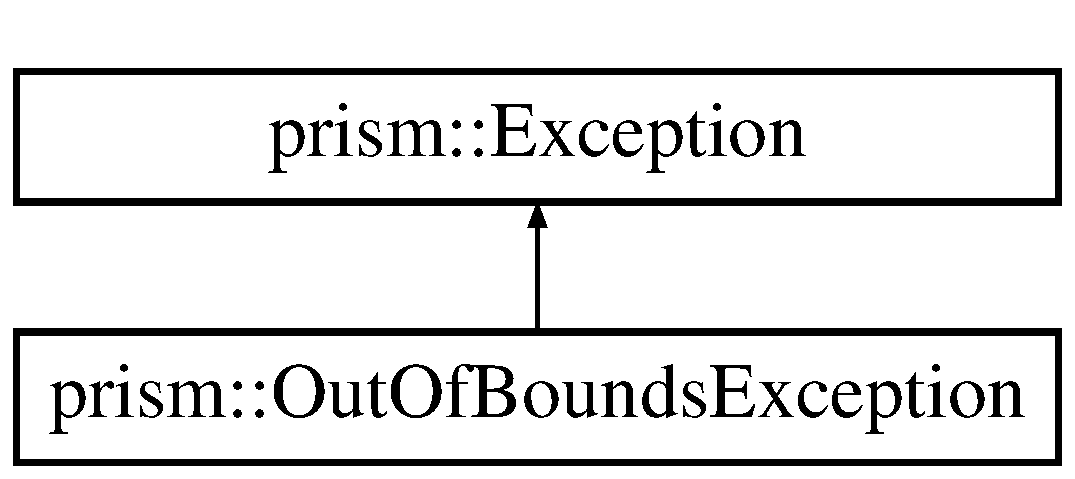
\includegraphics[height=2.000000cm]{classprism_1_1_out_of_bounds_exception}
\end{center}
\end{figure}
\subsection*{Public Member Functions}
\begin{DoxyCompactItemize}
\item 
\hyperlink{classprism_1_1_out_of_bounds_exception_a00b8a2c0b262a0f1be1de6daae008cb7}{Out\+Of\+Bounds\+Exception} (const int \hyperlink{classprism_1_1_out_of_bounds_exception_adc3c3d79e3211e6408d1b8670bd1766a}{index})
\item 
const int \hyperlink{classprism_1_1_out_of_bounds_exception_adc3c3d79e3211e6408d1b8670bd1766a}{index} () const 
\end{DoxyCompactItemize}
\subsection*{Additional Inherited Members}


\subsection{Constructor \& Destructor Documentation}
\index{prism\+::\+Out\+Of\+Bounds\+Exception@{prism\+::\+Out\+Of\+Bounds\+Exception}!Out\+Of\+Bounds\+Exception@{Out\+Of\+Bounds\+Exception}}
\index{Out\+Of\+Bounds\+Exception@{Out\+Of\+Bounds\+Exception}!prism\+::\+Out\+Of\+Bounds\+Exception@{prism\+::\+Out\+Of\+Bounds\+Exception}}
\subsubsection[{\texorpdfstring{Out\+Of\+Bounds\+Exception(const int index)}{OutOfBoundsException(const int index)}}]{\setlength{\rightskip}{0pt plus 5cm}prism\+::\+Out\+Of\+Bounds\+Exception\+::\+Out\+Of\+Bounds\+Exception (
\begin{DoxyParamCaption}
\item[{const int}]{index}
\end{DoxyParamCaption}
)\hspace{0.3cm}{\ttfamily [inline]}}\hypertarget{classprism_1_1_out_of_bounds_exception_a00b8a2c0b262a0f1be1de6daae008cb7}{}\label{classprism_1_1_out_of_bounds_exception_a00b8a2c0b262a0f1be1de6daae008cb7}


\subsection{Member Function Documentation}
\index{prism\+::\+Out\+Of\+Bounds\+Exception@{prism\+::\+Out\+Of\+Bounds\+Exception}!index@{index}}
\index{index@{index}!prism\+::\+Out\+Of\+Bounds\+Exception@{prism\+::\+Out\+Of\+Bounds\+Exception}}
\subsubsection[{\texorpdfstring{index() const }{index() const }}]{\setlength{\rightskip}{0pt plus 5cm}const int prism\+::\+Out\+Of\+Bounds\+Exception\+::index (
\begin{DoxyParamCaption}
{}
\end{DoxyParamCaption}
) const\hspace{0.3cm}{\ttfamily [inline]}}\hypertarget{classprism_1_1_out_of_bounds_exception_adc3c3d79e3211e6408d1b8670bd1766a}{}\label{classprism_1_1_out_of_bounds_exception_adc3c3d79e3211e6408d1b8670bd1766a}


The documentation for this class was generated from the following file\+:\begin{DoxyCompactItemize}
\item 
inc/prism/exceptions/\hyperlink{_out_of_bounds_exception_8h}{Out\+Of\+Bounds\+Exception.\+h}\end{DoxyCompactItemize}

\hypertarget{structprism_1_1output__iterator__tag}{}\section{prism\+:\+:output\+\_\+iterator\+\_\+tag Struct Reference}
\label{structprism_1_1output__iterator__tag}\index{prism\+::output\+\_\+iterator\+\_\+tag@{prism\+::output\+\_\+iterator\+\_\+tag}}


{\ttfamily \#include $<$Iterator.\+h$>$}



The documentation for this struct was generated from the following file\+:\begin{DoxyCompactItemize}
\item 
inc/\+Prism/containers/\hyperlink{_iterator_8h}{Iterator.\+h}\end{DoxyCompactItemize}

\hypertarget{classprism_1_1_overflow_exception}{}\section{prism\+:\+:Overflow\+Exception Class Reference}
\label{classprism_1_1_overflow_exception}\index{prism\+::\+Overflow\+Exception@{prism\+::\+Overflow\+Exception}}
Inheritance diagram for prism\+:\+:Overflow\+Exception\+:\begin{figure}[H]
\begin{center}
\leavevmode
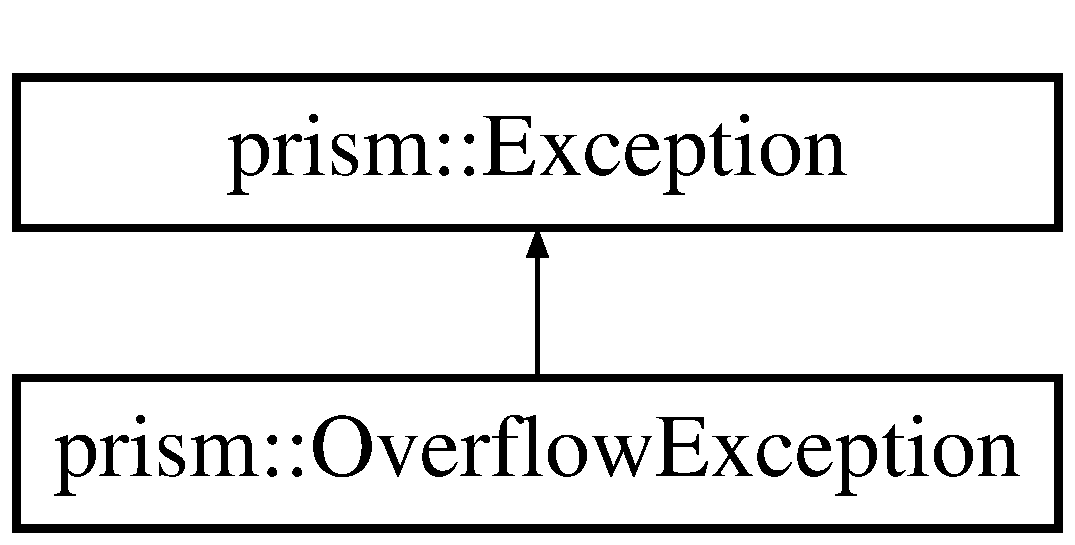
\includegraphics[height=2.000000cm]{classprism_1_1_overflow_exception}
\end{center}
\end{figure}
\subsection*{Public Member Functions}
\begin{DoxyCompactItemize}
\item 
\hyperlink{classprism_1_1_overflow_exception_a4969ca6350225f3cec0194f8f900eba4}{Overflow\+Exception} ()
\item 
\hyperlink{classprism_1_1_overflow_exception_a685bac60ef5028f7f36f7021da0a5c4f}{Overflow\+Exception} (const int index)
\end{DoxyCompactItemize}
\subsection*{Additional Inherited Members}


\subsection{Constructor \& Destructor Documentation}
\index{prism\+::\+Overflow\+Exception@{prism\+::\+Overflow\+Exception}!Overflow\+Exception@{Overflow\+Exception}}
\index{Overflow\+Exception@{Overflow\+Exception}!prism\+::\+Overflow\+Exception@{prism\+::\+Overflow\+Exception}}
\subsubsection[{\texorpdfstring{Overflow\+Exception()}{OverflowException()}}]{\setlength{\rightskip}{0pt plus 5cm}prism\+::\+Overflow\+Exception\+::\+Overflow\+Exception (
\begin{DoxyParamCaption}
{}
\end{DoxyParamCaption}
)\hspace{0.3cm}{\ttfamily [inline]}}\hypertarget{classprism_1_1_overflow_exception_a4969ca6350225f3cec0194f8f900eba4}{}\label{classprism_1_1_overflow_exception_a4969ca6350225f3cec0194f8f900eba4}
\index{prism\+::\+Overflow\+Exception@{prism\+::\+Overflow\+Exception}!Overflow\+Exception@{Overflow\+Exception}}
\index{Overflow\+Exception@{Overflow\+Exception}!prism\+::\+Overflow\+Exception@{prism\+::\+Overflow\+Exception}}
\subsubsection[{\texorpdfstring{Overflow\+Exception(const int index)}{OverflowException(const int index)}}]{\setlength{\rightskip}{0pt plus 5cm}prism\+::\+Overflow\+Exception\+::\+Overflow\+Exception (
\begin{DoxyParamCaption}
\item[{const int}]{index}
\end{DoxyParamCaption}
)\hspace{0.3cm}{\ttfamily [inline]}}\hypertarget{classprism_1_1_overflow_exception_a685bac60ef5028f7f36f7021da0a5c4f}{}\label{classprism_1_1_overflow_exception_a685bac60ef5028f7f36f7021da0a5c4f}


The documentation for this class was generated from the following file\+:\begin{DoxyCompactItemize}
\item 
\hyperlink{_overflow_exception_8h}{Overflow\+Exception.\+h}\end{DoxyCompactItemize}

\hypertarget{structprism_1_1pair}{}\section{prism\+:\+:pair$<$ T1, T2 $>$ Struct Template Reference}
\label{structprism_1_1pair}\index{prism\+::pair$<$ T1, T2 $>$@{prism\+::pair$<$ T1, T2 $>$}}
\subsection*{Public Types}
\begin{DoxyCompactItemize}
\item 
typedef T1 \hyperlink{structprism_1_1pair_a06bf88c0e5cb126378e584c53b81a030}{first\+\_\+type}
\item 
typedef T2 \hyperlink{structprism_1_1pair_a396e6009645d217824d896f8ba71c3da}{second\+\_\+type}
\end{DoxyCompactItemize}
\subsection*{Public Member Functions}
\begin{DoxyCompactItemize}
\item 
\hyperlink{structprism_1_1pair_ad0c7fedc65f0accae2489181e9404096}{pair} ()
\item 
\hyperlink{structprism_1_1pair_a387d4e7cf4e662bb25f4fc0b613548bc}{pair} (const T1 \&val1, const T2 \&val2)
\item 
virtual \hyperlink{structprism_1_1pair_a74836fc21bb693bae7e2afaa8c3d9258}{$\sim$pair} ()
\item 
\hyperlink{structprism_1_1pair}{pair}$<$ T1, T2 $>$ \& \hyperlink{structprism_1_1pair_aba4696cd0db8c77dd81a1a5187a06956}{operator=} (const \hyperlink{structprism_1_1pair}{pair} \&rhs)
\item 
{\footnotesize template$<$class T3 , class T4 $>$ }\\\hyperlink{structprism_1_1pair}{pair}$<$ T1, T2 $>$ \& \hyperlink{structprism_1_1pair_aeb7132de798fa55081a59a88b1bd9c08}{operator=} (const \hyperlink{structprism_1_1pair}{pair}$<$ T3, T4 $>$ \&rhs)
\end{DoxyCompactItemize}
\subsection*{Public Attributes}
\begin{DoxyCompactItemize}
\item 
T1 \hyperlink{structprism_1_1pair_a71d9cdb495193c9a7fcca8fdfbedc19d}{first}
\item 
T2 \hyperlink{structprism_1_1pair_a283ff14678f78c074f5f270943727ef3}{second}
\end{DoxyCompactItemize}
\subsection*{Friends}
\begin{DoxyCompactItemize}
\item 
const bool \hyperlink{structprism_1_1pair_ad7e2c2e8725c7ae941527a9859305b4a}{operator==} (const \hyperlink{structprism_1_1pair}{pair}$<$ T1, T2 $>$ \&p1, const \hyperlink{structprism_1_1pair}{pair}$<$ T1, T2 $>$ \&p2)
\item 
const bool \hyperlink{structprism_1_1pair_a5862e188719368db9f883f7a078f6778}{operator!=} (const \hyperlink{structprism_1_1pair}{pair}$<$ T1, T2 $>$ \&p1, const \hyperlink{structprism_1_1pair}{pair}$<$ T1, T2 $>$ \&p2)
\item 
std\+::ostream \& \hyperlink{structprism_1_1pair_ad79aaf53f199a130673f004de0ce4ea8}{operator$<$$<$} (std\+::ostream \&out, const \hyperlink{structprism_1_1pair}{pair} \&p)
\end{DoxyCompactItemize}


\subsection{Member Typedef Documentation}
\index{prism\+::pair@{prism\+::pair}!first\+\_\+type@{first\+\_\+type}}
\index{first\+\_\+type@{first\+\_\+type}!prism\+::pair@{prism\+::pair}}
\subsubsection[{\texorpdfstring{first\+\_\+type}{first_type}}]{\setlength{\rightskip}{0pt plus 5cm}template$<$class T1, class T2$>$ typedef T1 {\bf prism\+::pair}$<$ T1, T2 $>$\+::{\bf first\+\_\+type}}\hypertarget{structprism_1_1pair_a06bf88c0e5cb126378e584c53b81a030}{}\label{structprism_1_1pair_a06bf88c0e5cb126378e584c53b81a030}
\index{prism\+::pair@{prism\+::pair}!second\+\_\+type@{second\+\_\+type}}
\index{second\+\_\+type@{second\+\_\+type}!prism\+::pair@{prism\+::pair}}
\subsubsection[{\texorpdfstring{second\+\_\+type}{second_type}}]{\setlength{\rightskip}{0pt plus 5cm}template$<$class T1, class T2$>$ typedef T2 {\bf prism\+::pair}$<$ T1, T2 $>$\+::{\bf second\+\_\+type}}\hypertarget{structprism_1_1pair_a396e6009645d217824d896f8ba71c3da}{}\label{structprism_1_1pair_a396e6009645d217824d896f8ba71c3da}


\subsection{Constructor \& Destructor Documentation}
\index{prism\+::pair@{prism\+::pair}!pair@{pair}}
\index{pair@{pair}!prism\+::pair@{prism\+::pair}}
\subsubsection[{\texorpdfstring{pair()}{pair()}}]{\setlength{\rightskip}{0pt plus 5cm}template$<$class T1, class T2$>$ {\bf prism\+::pair}$<$ T1, T2 $>$\+::{\bf pair} (
\begin{DoxyParamCaption}
{}
\end{DoxyParamCaption}
)\hspace{0.3cm}{\ttfamily [inline]}}\hypertarget{structprism_1_1pair_ad0c7fedc65f0accae2489181e9404096}{}\label{structprism_1_1pair_ad0c7fedc65f0accae2489181e9404096}
\index{prism\+::pair@{prism\+::pair}!pair@{pair}}
\index{pair@{pair}!prism\+::pair@{prism\+::pair}}
\subsubsection[{\texorpdfstring{pair(const T1 \&val1, const T2 \&val2)}{pair(const T1 &val1, const T2 &val2)}}]{\setlength{\rightskip}{0pt plus 5cm}template$<$class T1, class T2$>$ {\bf prism\+::pair}$<$ T1, T2 $>$\+::{\bf pair} (
\begin{DoxyParamCaption}
\item[{const T1 \&}]{val1, }
\item[{const T2 \&}]{val2}
\end{DoxyParamCaption}
)\hspace{0.3cm}{\ttfamily [inline]}}\hypertarget{structprism_1_1pair_a387d4e7cf4e662bb25f4fc0b613548bc}{}\label{structprism_1_1pair_a387d4e7cf4e662bb25f4fc0b613548bc}
\index{prism\+::pair@{prism\+::pair}!````~pair@{$\sim$pair}}
\index{````~pair@{$\sim$pair}!prism\+::pair@{prism\+::pair}}
\subsubsection[{\texorpdfstring{$\sim$pair()}{~pair()}}]{\setlength{\rightskip}{0pt plus 5cm}template$<$class T1, class T2$>$ virtual {\bf prism\+::pair}$<$ T1, T2 $>$\+::$\sim${\bf pair} (
\begin{DoxyParamCaption}
{}
\end{DoxyParamCaption}
)\hspace{0.3cm}{\ttfamily [inline]}, {\ttfamily [virtual]}}\hypertarget{structprism_1_1pair_a74836fc21bb693bae7e2afaa8c3d9258}{}\label{structprism_1_1pair_a74836fc21bb693bae7e2afaa8c3d9258}


\subsection{Member Function Documentation}
\index{prism\+::pair@{prism\+::pair}!operator=@{operator=}}
\index{operator=@{operator=}!prism\+::pair@{prism\+::pair}}
\subsubsection[{\texorpdfstring{operator=(const pair \&rhs)}{operator=(const pair &rhs)}}]{\setlength{\rightskip}{0pt plus 5cm}template$<$class T1, class T2$>$ {\bf pair}$<$T1,T2$>$\& {\bf prism\+::pair}$<$ T1, T2 $>$\+::operator= (
\begin{DoxyParamCaption}
\item[{const {\bf pair}$<$ T1, T2 $>$ \&}]{rhs}
\end{DoxyParamCaption}
)\hspace{0.3cm}{\ttfamily [inline]}}\hypertarget{structprism_1_1pair_aba4696cd0db8c77dd81a1a5187a06956}{}\label{structprism_1_1pair_aba4696cd0db8c77dd81a1a5187a06956}
\index{prism\+::pair@{prism\+::pair}!operator=@{operator=}}
\index{operator=@{operator=}!prism\+::pair@{prism\+::pair}}
\subsubsection[{\texorpdfstring{operator=(const pair$<$ T3, T4 $>$ \&rhs)}{operator=(const pair< T3, T4 > &rhs)}}]{\setlength{\rightskip}{0pt plus 5cm}template$<$class T1, class T2$>$ template$<$class T3 , class T4 $>$ {\bf pair}$<$T1,T2$>$\& {\bf prism\+::pair}$<$ T1, T2 $>$\+::operator= (
\begin{DoxyParamCaption}
\item[{const {\bf pair}$<$ T3, T4 $>$ \&}]{rhs}
\end{DoxyParamCaption}
)\hspace{0.3cm}{\ttfamily [inline]}}\hypertarget{structprism_1_1pair_aeb7132de798fa55081a59a88b1bd9c08}{}\label{structprism_1_1pair_aeb7132de798fa55081a59a88b1bd9c08}


\subsection{Friends And Related Function Documentation}
\index{prism\+::pair@{prism\+::pair}!operator"!=@{operator"!=}}
\index{operator"!=@{operator"!=}!prism\+::pair@{prism\+::pair}}
\subsubsection[{\texorpdfstring{operator"!=}{operator!=}}]{\setlength{\rightskip}{0pt plus 5cm}template$<$class T1, class T2$>$ const bool operator!= (
\begin{DoxyParamCaption}
\item[{const {\bf pair}$<$ T1, T2 $>$ \&}]{p1, }
\item[{const {\bf pair}$<$ T1, T2 $>$ \&}]{p2}
\end{DoxyParamCaption}
)\hspace{0.3cm}{\ttfamily [friend]}}\hypertarget{structprism_1_1pair_a5862e188719368db9f883f7a078f6778}{}\label{structprism_1_1pair_a5862e188719368db9f883f7a078f6778}
\index{prism\+::pair@{prism\+::pair}!operator$<$$<$@{operator$<$$<$}}
\index{operator$<$$<$@{operator$<$$<$}!prism\+::pair@{prism\+::pair}}
\subsubsection[{\texorpdfstring{operator$<$$<$}{operator<<}}]{\setlength{\rightskip}{0pt plus 5cm}template$<$class T1, class T2$>$ std\+::ostream\& operator$<$$<$ (
\begin{DoxyParamCaption}
\item[{std\+::ostream \&}]{out, }
\item[{const {\bf pair}$<$ T1, T2 $>$ \&}]{p}
\end{DoxyParamCaption}
)\hspace{0.3cm}{\ttfamily [friend]}}\hypertarget{structprism_1_1pair_ad79aaf53f199a130673f004de0ce4ea8}{}\label{structprism_1_1pair_ad79aaf53f199a130673f004de0ce4ea8}
\index{prism\+::pair@{prism\+::pair}!operator==@{operator==}}
\index{operator==@{operator==}!prism\+::pair@{prism\+::pair}}
\subsubsection[{\texorpdfstring{operator==}{operator==}}]{\setlength{\rightskip}{0pt plus 5cm}template$<$class T1, class T2$>$ const bool operator== (
\begin{DoxyParamCaption}
\item[{const {\bf pair}$<$ T1, T2 $>$ \&}]{p1, }
\item[{const {\bf pair}$<$ T1, T2 $>$ \&}]{p2}
\end{DoxyParamCaption}
)\hspace{0.3cm}{\ttfamily [friend]}}\hypertarget{structprism_1_1pair_ad7e2c2e8725c7ae941527a9859305b4a}{}\label{structprism_1_1pair_ad7e2c2e8725c7ae941527a9859305b4a}


\subsection{Member Data Documentation}
\index{prism\+::pair@{prism\+::pair}!first@{first}}
\index{first@{first}!prism\+::pair@{prism\+::pair}}
\subsubsection[{\texorpdfstring{first}{first}}]{\setlength{\rightskip}{0pt plus 5cm}template$<$class T1, class T2$>$ T1 {\bf prism\+::pair}$<$ T1, T2 $>$\+::first}\hypertarget{structprism_1_1pair_a71d9cdb495193c9a7fcca8fdfbedc19d}{}\label{structprism_1_1pair_a71d9cdb495193c9a7fcca8fdfbedc19d}
\index{prism\+::pair@{prism\+::pair}!second@{second}}
\index{second@{second}!prism\+::pair@{prism\+::pair}}
\subsubsection[{\texorpdfstring{second}{second}}]{\setlength{\rightskip}{0pt plus 5cm}template$<$class T1, class T2$>$ T2 {\bf prism\+::pair}$<$ T1, T2 $>$\+::second}\hypertarget{structprism_1_1pair_a283ff14678f78c074f5f270943727ef3}{}\label{structprism_1_1pair_a283ff14678f78c074f5f270943727ef3}


The documentation for this struct was generated from the following file\+:\begin{DoxyCompactItemize}
\item 
\hyperlink{_pair_8h}{Pair.\+h}\end{DoxyCompactItemize}

\hypertarget{classprism_1_1_point}{}\section{prism\+:\+:Point Class Reference}
\label{classprism_1_1_point}\index{prism\+::\+Point@{prism\+::\+Point}}


{\ttfamily \#include $<$Point.\+h$>$}

\subsection*{Public Member Functions}
\begin{DoxyCompactItemize}
\item 
\hyperlink{classprism_1_1_point_a505a19bd681a9e195f8bf9dbd3c445c7}{Point} (void)
\item 
\hyperlink{classprism_1_1_point_a93bfdd8fa48253786030802190577129}{Point} (const int \hyperlink{classprism_1_1_point_a725d8721ccf4e59ce9a912490e9487f9}{x}, const int \hyperlink{classprism_1_1_point_ac3283efaa56d37b9d69b7ff5e9d5c2f4}{y})
\item 
\hyperlink{classprism_1_1_point_af09a25c46be47b8c4566b15ddac632b0}{Point} (const \hyperlink{classprism_1_1_point}{Point} \&\hyperlink{namespaceprism_ae776f4cd825f79e7af1cf6ee1d90a209}{copy})
\item 
\hyperlink{classprism_1_1_point_a948aa05b80053c019bf963315a2cea8a}{$\sim$\+Point} (void)
\item 
void \hyperlink{classprism_1_1_point_abda32c4f2e16a5a3276949732992f911}{reset} ()
\item 
const bool \hyperlink{classprism_1_1_point_a426d00c2d9d582723ed69e1a73034641}{is\+Reset} () const 
\item 
void \hyperlink{classprism_1_1_point_ac327d98f8dfc1768a6aae63a144cf2fd}{set} (const int \hyperlink{classprism_1_1_point_a725d8721ccf4e59ce9a912490e9487f9}{x}, const int \hyperlink{classprism_1_1_point_ac3283efaa56d37b9d69b7ff5e9d5c2f4}{y})
\item 
void \hyperlink{classprism_1_1_point_a39aac064dac78373b3be254ab2bc6ab4}{setX} (const int \hyperlink{classprism_1_1_point_a725d8721ccf4e59ce9a912490e9487f9}{x})
\item 
void \hyperlink{classprism_1_1_point_afc2fc43295a911175d7e709b80dc2068}{setY} (const int \hyperlink{classprism_1_1_point_ac3283efaa56d37b9d69b7ff5e9d5c2f4}{y})
\item 
const int \hyperlink{classprism_1_1_point_a725d8721ccf4e59ce9a912490e9487f9}{x} () const 
\item 
const int \hyperlink{classprism_1_1_point_ac3283efaa56d37b9d69b7ff5e9d5c2f4}{y} () const 
\item 
int \& \hyperlink{classprism_1_1_point_abcbcac675e56f63e69d7fc165fd66106}{rx} ()
\item 
int \& \hyperlink{classprism_1_1_point_a380a0a615af10ec2392a472ca11325d7}{ry} ()
\item 
\hyperlink{classprism_1_1_point}{Point} \& \hyperlink{classprism_1_1_point_a7e3386be01e28ac9db673c91384a0d53}{operator=} (const \hyperlink{classprism_1_1_point}{Point} \&p)
\item 
\hyperlink{classprism_1_1_point}{Point} \& \hyperlink{classprism_1_1_point_a3df2e80f1554f772e14d1b4ecc55e4a9}{operator+=} (const \hyperlink{classprism_1_1_point}{Point} \&p)
\item 
\hyperlink{classprism_1_1_point}{Point} \& \hyperlink{classprism_1_1_point_a6d407a4ac17b13e941b31519d5f7a8a3}{operator-\/=} (const \hyperlink{classprism_1_1_point}{Point} \&p)
\item 
\hyperlink{classprism_1_1_point}{Point} \& \hyperlink{classprism_1_1_point_a170f9053e8e7c3319c86de5af5843ee4}{operator$\ast$=} (const float factor)
\item 
\hyperlink{classprism_1_1_point}{Point} \& \hyperlink{classprism_1_1_point_ab036f1dc222dd33a580df59a4170f60f}{operator$\ast$=} (const int factor)
\item 
\hyperlink{classprism_1_1_point}{Point} \& \hyperlink{classprism_1_1_point_a6b5e3e019f8cf484d372fc355e6c7a64}{operator/=} (const float divisor)
\item 
\hyperlink{classprism_1_1_point}{Point} \& \hyperlink{classprism_1_1_point_a6d152f61b02e2a62b356627079c15089}{operator/=} (const int divisor)
\end{DoxyCompactItemize}
\subsection*{Friends}
\begin{DoxyCompactItemize}
\item 
std\+::ostream \& \hyperlink{classprism_1_1_point_aa818efa680e0d94ce91173ccb4b7aa08}{operator$<$$<$} (std\+::ostream \&out, const \hyperlink{classprism_1_1_point}{Point} \&p)
\item 
\hyperlink{classprism_1_1_point}{Point} \hyperlink{classprism_1_1_point_af9fd2d27c54f694ce11ba1e9df0b58f1}{operator+} (const \hyperlink{classprism_1_1_point}{Point} \&p1, const \hyperlink{classprism_1_1_point}{Point} \&p2)
\item 
\hyperlink{classprism_1_1_point}{Point} \hyperlink{classprism_1_1_point_aff59dfb837229858286c1652bd9a8e40}{operator-\/} (const \hyperlink{classprism_1_1_point}{Point} \&p1, const \hyperlink{classprism_1_1_point}{Point} \&p2)
\item 
\hyperlink{classprism_1_1_point}{Point} \hyperlink{classprism_1_1_point_a3fff687aebd2165ff57e237363953f36}{operator$\ast$} (const \hyperlink{classprism_1_1_point}{Point} \&p, const int factor)
\item 
\hyperlink{classprism_1_1_point}{Point} \hyperlink{classprism_1_1_point_a6a69d67bbbf8aa38b38c71440a8341cc}{operator$\ast$} (const \hyperlink{classprism_1_1_point}{Point} \&p, const float factor)
\item 
\hyperlink{classprism_1_1_point}{Point} \hyperlink{classprism_1_1_point_ab4cfccba8d1b3c1d29dedb1d729ecaaf}{operator$\ast$} (const int factor, const \hyperlink{classprism_1_1_point}{Point} \&p)
\item 
\hyperlink{classprism_1_1_point}{Point} \hyperlink{classprism_1_1_point_a3141285de569d8565c2ae20e3155de14}{operator$\ast$} (const float factor, const \hyperlink{classprism_1_1_point}{Point} \&p)
\item 
\hyperlink{classprism_1_1_point}{Point} \hyperlink{classprism_1_1_point_adeafa81d7b8a890cbe28b9159aad4eb4}{operator/} (const \hyperlink{classprism_1_1_point}{Point} \&p, const float divisor)
\item 
bool \hyperlink{classprism_1_1_point_a2c5b474dd81e3ce9b80b206ea32deaae}{operator==} (const \hyperlink{classprism_1_1_point}{Point} \&p1, const \hyperlink{classprism_1_1_point}{Point} \&p2)
\item 
bool \hyperlink{classprism_1_1_point_a694df69725e33fcd64fd0942c6bb5e82}{operator!=} (const \hyperlink{classprism_1_1_point}{Point} \&p1, const \hyperlink{classprism_1_1_point}{Point} \&p2)
\end{DoxyCompactItemize}


\subsection{Constructor \& Destructor Documentation}
\index{prism\+::\+Point@{prism\+::\+Point}!Point@{Point}}
\index{Point@{Point}!prism\+::\+Point@{prism\+::\+Point}}
\subsubsection[{\texorpdfstring{Point(void)}{Point(void)}}]{\setlength{\rightskip}{0pt plus 5cm}prism\+::\+Point\+::\+Point (
\begin{DoxyParamCaption}
\item[{void}]{}
\end{DoxyParamCaption}
)}\hypertarget{classprism_1_1_point_a505a19bd681a9e195f8bf9dbd3c445c7}{}\label{classprism_1_1_point_a505a19bd681a9e195f8bf9dbd3c445c7}
Default constructor \index{prism\+::\+Point@{prism\+::\+Point}!Point@{Point}}
\index{Point@{Point}!prism\+::\+Point@{prism\+::\+Point}}
\subsubsection[{\texorpdfstring{Point(const int x, const int y)}{Point(const int x, const int y)}}]{\setlength{\rightskip}{0pt plus 5cm}prism\+::\+Point\+::\+Point (
\begin{DoxyParamCaption}
\item[{const int}]{x, }
\item[{const int}]{y}
\end{DoxyParamCaption}
)}\hypertarget{classprism_1_1_point_a93bfdd8fa48253786030802190577129}{}\label{classprism_1_1_point_a93bfdd8fa48253786030802190577129}
Constructor override \index{prism\+::\+Point@{prism\+::\+Point}!Point@{Point}}
\index{Point@{Point}!prism\+::\+Point@{prism\+::\+Point}}
\subsubsection[{\texorpdfstring{Point(const Point \&copy)}{Point(const Point &copy)}}]{\setlength{\rightskip}{0pt plus 5cm}prism\+::\+Point\+::\+Point (
\begin{DoxyParamCaption}
\item[{const {\bf Point} \&}]{copy}
\end{DoxyParamCaption}
)}\hypertarget{classprism_1_1_point_af09a25c46be47b8c4566b15ddac632b0}{}\label{classprism_1_1_point_af09a25c46be47b8c4566b15ddac632b0}
\index{prism\+::\+Point@{prism\+::\+Point}!````~Point@{$\sim$\+Point}}
\index{````~Point@{$\sim$\+Point}!prism\+::\+Point@{prism\+::\+Point}}
\subsubsection[{\texorpdfstring{$\sim$\+Point(void)}{~Point(void)}}]{\setlength{\rightskip}{0pt plus 5cm}prism\+::\+Point\+::$\sim$\+Point (
\begin{DoxyParamCaption}
\item[{void}]{}
\end{DoxyParamCaption}
)}\hypertarget{classprism_1_1_point_a948aa05b80053c019bf963315a2cea8a}{}\label{classprism_1_1_point_a948aa05b80053c019bf963315a2cea8a}
Virtual destructor 

\subsection{Member Function Documentation}
\index{prism\+::\+Point@{prism\+::\+Point}!is\+Reset@{is\+Reset}}
\index{is\+Reset@{is\+Reset}!prism\+::\+Point@{prism\+::\+Point}}
\subsubsection[{\texorpdfstring{is\+Reset() const }{isReset() const }}]{\setlength{\rightskip}{0pt plus 5cm}const bool prism\+::\+Point\+::is\+Reset (
\begin{DoxyParamCaption}
{}
\end{DoxyParamCaption}
) const}\hypertarget{classprism_1_1_point_a426d00c2d9d582723ed69e1a73034641}{}\label{classprism_1_1_point_a426d00c2d9d582723ed69e1a73034641}
Returns true if x=0 and y=0, false if not \index{prism\+::\+Point@{prism\+::\+Point}!operator$\ast$=@{operator$\ast$=}}
\index{operator$\ast$=@{operator$\ast$=}!prism\+::\+Point@{prism\+::\+Point}}
\subsubsection[{\texorpdfstring{operator$\ast$=(const float factor)}{operator*=(const float factor)}}]{\setlength{\rightskip}{0pt plus 5cm}{\bf Point} \& prism\+::\+Point\+::operator$\ast$= (
\begin{DoxyParamCaption}
\item[{const float}]{factor}
\end{DoxyParamCaption}
)}\hypertarget{classprism_1_1_point_a170f9053e8e7c3319c86de5af5843ee4}{}\label{classprism_1_1_point_a170f9053e8e7c3319c86de5af5843ee4}
Multiplies this point\textquotesingle{}s components by the given factor and returns a reference to this point. Note\+: the x and y components are rounded to the nearest integer as they are stored as ints internally. Use \hyperlink{classprism_1_1_pointf}{Pointf} for floating point accuracy instead. \index{prism\+::\+Point@{prism\+::\+Point}!operator$\ast$=@{operator$\ast$=}}
\index{operator$\ast$=@{operator$\ast$=}!prism\+::\+Point@{prism\+::\+Point}}
\subsubsection[{\texorpdfstring{operator$\ast$=(const int factor)}{operator*=(const int factor)}}]{\setlength{\rightskip}{0pt plus 5cm}{\bf Point} \& prism\+::\+Point\+::operator$\ast$= (
\begin{DoxyParamCaption}
\item[{const int}]{factor}
\end{DoxyParamCaption}
)}\hypertarget{classprism_1_1_point_ab036f1dc222dd33a580df59a4170f60f}{}\label{classprism_1_1_point_ab036f1dc222dd33a580df59a4170f60f}
Multiplies this point\textquotesingle{}s coordinates by the given factor and returns a reference to this point. \index{prism\+::\+Point@{prism\+::\+Point}!operator+=@{operator+=}}
\index{operator+=@{operator+=}!prism\+::\+Point@{prism\+::\+Point}}
\subsubsection[{\texorpdfstring{operator+=(const Point \&p)}{operator+=(const Point &p)}}]{\setlength{\rightskip}{0pt plus 5cm}{\bf Point} \& prism\+::\+Point\+::operator+= (
\begin{DoxyParamCaption}
\item[{const {\bf Point} \&}]{p}
\end{DoxyParamCaption}
)}\hypertarget{classprism_1_1_point_a3df2e80f1554f772e14d1b4ecc55e4a9}{}\label{classprism_1_1_point_a3df2e80f1554f772e14d1b4ecc55e4a9}
Returns a reference to this point after adding p to it \index{prism\+::\+Point@{prism\+::\+Point}!operator-\/=@{operator-\/=}}
\index{operator-\/=@{operator-\/=}!prism\+::\+Point@{prism\+::\+Point}}
\subsubsection[{\texorpdfstring{operator-\/=(const Point \&p)}{operator-=(const Point &p)}}]{\setlength{\rightskip}{0pt plus 5cm}{\bf Point} \& prism\+::\+Point\+::operator-\/= (
\begin{DoxyParamCaption}
\item[{const {\bf Point} \&}]{p}
\end{DoxyParamCaption}
)}\hypertarget{classprism_1_1_point_a6d407a4ac17b13e941b31519d5f7a8a3}{}\label{classprism_1_1_point_a6d407a4ac17b13e941b31519d5f7a8a3}
Returns a reference to this point after subtracting p from it \index{prism\+::\+Point@{prism\+::\+Point}!operator/=@{operator/=}}
\index{operator/=@{operator/=}!prism\+::\+Point@{prism\+::\+Point}}
\subsubsection[{\texorpdfstring{operator/=(const float divisor)}{operator/=(const float divisor)}}]{\setlength{\rightskip}{0pt plus 5cm}{\bf Point} \& prism\+::\+Point\+::operator/= (
\begin{DoxyParamCaption}
\item[{const float}]{divisor}
\end{DoxyParamCaption}
)}\hypertarget{classprism_1_1_point_a6b5e3e019f8cf484d372fc355e6c7a64}{}\label{classprism_1_1_point_a6b5e3e019f8cf484d372fc355e6c7a64}
Multiplies this point\textquotesingle{}s coordinates by the given factor and returns a reference to this point Note\+: the x and y components are rounded to the nearest integer as they are stored as ints internally. Use \hyperlink{classprism_1_1_pointf}{Pointf} for floating point accuracy instead. \index{prism\+::\+Point@{prism\+::\+Point}!operator/=@{operator/=}}
\index{operator/=@{operator/=}!prism\+::\+Point@{prism\+::\+Point}}
\subsubsection[{\texorpdfstring{operator/=(const int divisor)}{operator/=(const int divisor)}}]{\setlength{\rightskip}{0pt plus 5cm}{\bf Point} \& prism\+::\+Point\+::operator/= (
\begin{DoxyParamCaption}
\item[{const int}]{divisor}
\end{DoxyParamCaption}
)}\hypertarget{classprism_1_1_point_a6d152f61b02e2a62b356627079c15089}{}\label{classprism_1_1_point_a6d152f61b02e2a62b356627079c15089}
Divides this point\textquotesingle{}s coordinates by the given factor and returns a reference to this point. Note\+: the x and y components are rounded to the nearest integer as they are stored as ints internally. Use \hyperlink{classprism_1_1_pointf}{Pointf} for floating point accuracy instead. \index{prism\+::\+Point@{prism\+::\+Point}!operator=@{operator=}}
\index{operator=@{operator=}!prism\+::\+Point@{prism\+::\+Point}}
\subsubsection[{\texorpdfstring{operator=(const Point \&p)}{operator=(const Point &p)}}]{\setlength{\rightskip}{0pt plus 5cm}{\bf Point} \& prism\+::\+Point\+::operator= (
\begin{DoxyParamCaption}
\item[{const {\bf Point} \&}]{p}
\end{DoxyParamCaption}
)}\hypertarget{classprism_1_1_point_a7e3386be01e28ac9db673c91384a0d53}{}\label{classprism_1_1_point_a7e3386be01e28ac9db673c91384a0d53}
\index{prism\+::\+Point@{prism\+::\+Point}!reset@{reset}}
\index{reset@{reset}!prism\+::\+Point@{prism\+::\+Point}}
\subsubsection[{\texorpdfstring{reset()}{reset()}}]{\setlength{\rightskip}{0pt plus 5cm}void prism\+::\+Point\+::reset (
\begin{DoxyParamCaption}
{}
\end{DoxyParamCaption}
)}\hypertarget{classprism_1_1_point_abda32c4f2e16a5a3276949732992f911}{}\label{classprism_1_1_point_abda32c4f2e16a5a3276949732992f911}
Resets this point back to x=y=0 \index{prism\+::\+Point@{prism\+::\+Point}!rx@{rx}}
\index{rx@{rx}!prism\+::\+Point@{prism\+::\+Point}}
\subsubsection[{\texorpdfstring{rx()}{rx()}}]{\setlength{\rightskip}{0pt plus 5cm}int \& prism\+::\+Point\+::rx (
\begin{DoxyParamCaption}
{}
\end{DoxyParamCaption}
)}\hypertarget{classprism_1_1_point_abcbcac675e56f63e69d7fc165fd66106}{}\label{classprism_1_1_point_abcbcac675e56f63e69d7fc165fd66106}
Returns a reference to the x component allowing direct manipulation i.\+e. point.\+rx() += 5 \index{prism\+::\+Point@{prism\+::\+Point}!ry@{ry}}
\index{ry@{ry}!prism\+::\+Point@{prism\+::\+Point}}
\subsubsection[{\texorpdfstring{ry()}{ry()}}]{\setlength{\rightskip}{0pt plus 5cm}int \& prism\+::\+Point\+::ry (
\begin{DoxyParamCaption}
{}
\end{DoxyParamCaption}
)}\hypertarget{classprism_1_1_point_a380a0a615af10ec2392a472ca11325d7}{}\label{classprism_1_1_point_a380a0a615af10ec2392a472ca11325d7}
Returns a reference to the y component allowing direct manipulation i.\+e. point.\+ry() += 5 \index{prism\+::\+Point@{prism\+::\+Point}!set@{set}}
\index{set@{set}!prism\+::\+Point@{prism\+::\+Point}}
\subsubsection[{\texorpdfstring{set(const int x, const int y)}{set(const int x, const int y)}}]{\setlength{\rightskip}{0pt plus 5cm}void prism\+::\+Point\+::set (
\begin{DoxyParamCaption}
\item[{const int}]{x, }
\item[{const int}]{y}
\end{DoxyParamCaption}
)}\hypertarget{classprism_1_1_point_ac327d98f8dfc1768a6aae63a144cf2fd}{}\label{classprism_1_1_point_ac327d98f8dfc1768a6aae63a144cf2fd}
Convenience method that sets x and y simultaineously \index{prism\+::\+Point@{prism\+::\+Point}!setX@{setX}}
\index{setX@{setX}!prism\+::\+Point@{prism\+::\+Point}}
\subsubsection[{\texorpdfstring{set\+X(const int x)}{setX(const int x)}}]{\setlength{\rightskip}{0pt plus 5cm}void prism\+::\+Point\+::setX (
\begin{DoxyParamCaption}
\item[{const int}]{x}
\end{DoxyParamCaption}
)}\hypertarget{classprism_1_1_point_a39aac064dac78373b3be254ab2bc6ab4}{}\label{classprism_1_1_point_a39aac064dac78373b3be254ab2bc6ab4}
Sets the x component \index{prism\+::\+Point@{prism\+::\+Point}!setY@{setY}}
\index{setY@{setY}!prism\+::\+Point@{prism\+::\+Point}}
\subsubsection[{\texorpdfstring{set\+Y(const int y)}{setY(const int y)}}]{\setlength{\rightskip}{0pt plus 5cm}void prism\+::\+Point\+::setY (
\begin{DoxyParamCaption}
\item[{const int}]{y}
\end{DoxyParamCaption}
)}\hypertarget{classprism_1_1_point_afc2fc43295a911175d7e709b80dc2068}{}\label{classprism_1_1_point_afc2fc43295a911175d7e709b80dc2068}
Sets the y component \index{prism\+::\+Point@{prism\+::\+Point}!x@{x}}
\index{x@{x}!prism\+::\+Point@{prism\+::\+Point}}
\subsubsection[{\texorpdfstring{x() const }{x() const }}]{\setlength{\rightskip}{0pt plus 5cm}const int prism\+::\+Point\+::x (
\begin{DoxyParamCaption}
{}
\end{DoxyParamCaption}
) const}\hypertarget{classprism_1_1_point_a725d8721ccf4e59ce9a912490e9487f9}{}\label{classprism_1_1_point_a725d8721ccf4e59ce9a912490e9487f9}
Returns the x component \index{prism\+::\+Point@{prism\+::\+Point}!y@{y}}
\index{y@{y}!prism\+::\+Point@{prism\+::\+Point}}
\subsubsection[{\texorpdfstring{y() const }{y() const }}]{\setlength{\rightskip}{0pt plus 5cm}const int prism\+::\+Point\+::y (
\begin{DoxyParamCaption}
{}
\end{DoxyParamCaption}
) const}\hypertarget{classprism_1_1_point_ac3283efaa56d37b9d69b7ff5e9d5c2f4}{}\label{classprism_1_1_point_ac3283efaa56d37b9d69b7ff5e9d5c2f4}
Returns the y component 

\subsection{Friends And Related Function Documentation}
\index{prism\+::\+Point@{prism\+::\+Point}!operator"!=@{operator"!=}}
\index{operator"!=@{operator"!=}!prism\+::\+Point@{prism\+::\+Point}}
\subsubsection[{\texorpdfstring{operator"!=}{operator!=}}]{\setlength{\rightskip}{0pt plus 5cm}bool operator!= (
\begin{DoxyParamCaption}
\item[{const {\bf Point} \&}]{p1, }
\item[{const {\bf Point} \&}]{p2}
\end{DoxyParamCaption}
)\hspace{0.3cm}{\ttfamily [friend]}}\hypertarget{classprism_1_1_point_a694df69725e33fcd64fd0942c6bb5e82}{}\label{classprism_1_1_point_a694df69725e33fcd64fd0942c6bb5e82}
Returns true if x or y of p1 and p2 are not equal, false if not \index{prism\+::\+Point@{prism\+::\+Point}!operator$\ast$@{operator$\ast$}}
\index{operator$\ast$@{operator$\ast$}!prism\+::\+Point@{prism\+::\+Point}}
\subsubsection[{\texorpdfstring{operator$\ast$}{operator*}}]{\setlength{\rightskip}{0pt plus 5cm}{\bf Point} operator$\ast$ (
\begin{DoxyParamCaption}
\item[{const {\bf Point} \&}]{p, }
\item[{const int}]{factor}
\end{DoxyParamCaption}
)\hspace{0.3cm}{\ttfamily [friend]}}\hypertarget{classprism_1_1_point_a3fff687aebd2165ff57e237363953f36}{}\label{classprism_1_1_point_a3fff687aebd2165ff57e237363953f36}
Returns a \hyperlink{classprism_1_1_point}{Point} object that is formed by multiplying the components of p by the int factor \index{prism\+::\+Point@{prism\+::\+Point}!operator$\ast$@{operator$\ast$}}
\index{operator$\ast$@{operator$\ast$}!prism\+::\+Point@{prism\+::\+Point}}
\subsubsection[{\texorpdfstring{operator$\ast$}{operator*}}]{\setlength{\rightskip}{0pt plus 5cm}{\bf Point} operator$\ast$ (
\begin{DoxyParamCaption}
\item[{const {\bf Point} \&}]{p, }
\item[{const float}]{factor}
\end{DoxyParamCaption}
)\hspace{0.3cm}{\ttfamily [friend]}}\hypertarget{classprism_1_1_point_a6a69d67bbbf8aa38b38c71440a8341cc}{}\label{classprism_1_1_point_a6a69d67bbbf8aa38b38c71440a8341cc}
Returns a \hyperlink{classprism_1_1_point}{Point} object that is formed by multiplying the components of p by the float factor Note\+: the x and y components are rounded to the nearest integer as they are stored as ints internally. Use \hyperlink{classprism_1_1_pointf}{Pointf} for floating point accuracy instead. \index{prism\+::\+Point@{prism\+::\+Point}!operator$\ast$@{operator$\ast$}}
\index{operator$\ast$@{operator$\ast$}!prism\+::\+Point@{prism\+::\+Point}}
\subsubsection[{\texorpdfstring{operator$\ast$}{operator*}}]{\setlength{\rightskip}{0pt plus 5cm}{\bf Point} operator$\ast$ (
\begin{DoxyParamCaption}
\item[{const int}]{factor, }
\item[{const {\bf Point} \&}]{p}
\end{DoxyParamCaption}
)\hspace{0.3cm}{\ttfamily [friend]}}\hypertarget{classprism_1_1_point_ab4cfccba8d1b3c1d29dedb1d729ecaaf}{}\label{classprism_1_1_point_ab4cfccba8d1b3c1d29dedb1d729ecaaf}
Returns a \hyperlink{classprism_1_1_point}{Point} object that is formed by multiplying the components of p by the int factor \index{prism\+::\+Point@{prism\+::\+Point}!operator$\ast$@{operator$\ast$}}
\index{operator$\ast$@{operator$\ast$}!prism\+::\+Point@{prism\+::\+Point}}
\subsubsection[{\texorpdfstring{operator$\ast$}{operator*}}]{\setlength{\rightskip}{0pt plus 5cm}{\bf Point} operator$\ast$ (
\begin{DoxyParamCaption}
\item[{const float}]{factor, }
\item[{const {\bf Point} \&}]{p}
\end{DoxyParamCaption}
)\hspace{0.3cm}{\ttfamily [friend]}}\hypertarget{classprism_1_1_point_a3141285de569d8565c2ae20e3155de14}{}\label{classprism_1_1_point_a3141285de569d8565c2ae20e3155de14}
Returns a \hyperlink{classprism_1_1_point}{Point} object that is formed by multiplying the components of p by the float factor Note\+: the x and y components are rounded to the nearest integer as they are stored as ints internally. Use \hyperlink{classprism_1_1_pointf}{Pointf} for floating point accuracy instead. \index{prism\+::\+Point@{prism\+::\+Point}!operator+@{operator+}}
\index{operator+@{operator+}!prism\+::\+Point@{prism\+::\+Point}}
\subsubsection[{\texorpdfstring{operator+}{operator+}}]{\setlength{\rightskip}{0pt plus 5cm}{\bf Point} operator+ (
\begin{DoxyParamCaption}
\item[{const {\bf Point} \&}]{p1, }
\item[{const {\bf Point} \&}]{p2}
\end{DoxyParamCaption}
)\hspace{0.3cm}{\ttfamily [friend]}}\hypertarget{classprism_1_1_point_af9fd2d27c54f694ce11ba1e9df0b58f1}{}\label{classprism_1_1_point_af9fd2d27c54f694ce11ba1e9df0b58f1}
Returns a \hyperlink{classprism_1_1_point}{Point} object that is the sum of the components of p1 and p2 \index{prism\+::\+Point@{prism\+::\+Point}!operator-\/@{operator-\/}}
\index{operator-\/@{operator-\/}!prism\+::\+Point@{prism\+::\+Point}}
\subsubsection[{\texorpdfstring{operator-\/}{operator-}}]{\setlength{\rightskip}{0pt plus 5cm}{\bf Point} operator-\/ (
\begin{DoxyParamCaption}
\item[{const {\bf Point} \&}]{p1, }
\item[{const {\bf Point} \&}]{p2}
\end{DoxyParamCaption}
)\hspace{0.3cm}{\ttfamily [friend]}}\hypertarget{classprism_1_1_point_aff59dfb837229858286c1652bd9a8e40}{}\label{classprism_1_1_point_aff59dfb837229858286c1652bd9a8e40}
Returns a \hyperlink{classprism_1_1_point}{Point} object that is formed by subtracting the components of p2 from p1 \index{prism\+::\+Point@{prism\+::\+Point}!operator/@{operator/}}
\index{operator/@{operator/}!prism\+::\+Point@{prism\+::\+Point}}
\subsubsection[{\texorpdfstring{operator/}{operator/}}]{\setlength{\rightskip}{0pt plus 5cm}{\bf Point} operator/ (
\begin{DoxyParamCaption}
\item[{const {\bf Point} \&}]{p, }
\item[{const float}]{divisor}
\end{DoxyParamCaption}
)\hspace{0.3cm}{\ttfamily [friend]}}\hypertarget{classprism_1_1_point_adeafa81d7b8a890cbe28b9159aad4eb4}{}\label{classprism_1_1_point_adeafa81d7b8a890cbe28b9159aad4eb4}
Returns a \hyperlink{classprism_1_1_point}{Point} object that is formed by dividing the components of p1 by the components of p2 \index{prism\+::\+Point@{prism\+::\+Point}!operator$<$$<$@{operator$<$$<$}}
\index{operator$<$$<$@{operator$<$$<$}!prism\+::\+Point@{prism\+::\+Point}}
\subsubsection[{\texorpdfstring{operator$<$$<$}{operator<<}}]{\setlength{\rightskip}{0pt plus 5cm}std\+::ostream\& operator$<$$<$ (
\begin{DoxyParamCaption}
\item[{std\+::ostream \&}]{out, }
\item[{const {\bf Point} \&}]{p}
\end{DoxyParamCaption}
)\hspace{0.3cm}{\ttfamily [friend]}}\hypertarget{classprism_1_1_point_aa818efa680e0d94ce91173ccb4b7aa08}{}\label{classprism_1_1_point_aa818efa680e0d94ce91173ccb4b7aa08}
Returns an ostream object that allows this object to printed with std\+::cout \index{prism\+::\+Point@{prism\+::\+Point}!operator==@{operator==}}
\index{operator==@{operator==}!prism\+::\+Point@{prism\+::\+Point}}
\subsubsection[{\texorpdfstring{operator==}{operator==}}]{\setlength{\rightskip}{0pt plus 5cm}bool operator== (
\begin{DoxyParamCaption}
\item[{const {\bf Point} \&}]{p1, }
\item[{const {\bf Point} \&}]{p2}
\end{DoxyParamCaption}
)\hspace{0.3cm}{\ttfamily [friend]}}\hypertarget{classprism_1_1_point_a2c5b474dd81e3ce9b80b206ea32deaae}{}\label{classprism_1_1_point_a2c5b474dd81e3ce9b80b206ea32deaae}
Returns true if x and y of p1 and p2 are equal, false if not 

The documentation for this class was generated from the following files\+:\begin{DoxyCompactItemize}
\item 
inc/prism/\hyperlink{_point_8h}{Point.\+h}\item 
src/prism/\hyperlink{_point_8cpp}{Point.\+cpp}\end{DoxyCompactItemize}

\hypertarget{classprism_1_1_pointf}{}\section{prism\+:\+:Pointf Class Reference}
\label{classprism_1_1_pointf}\index{prism\+::\+Pointf@{prism\+::\+Pointf}}
\subsection*{Public Member Functions}
\begin{DoxyCompactItemize}
\item 
\hyperlink{classprism_1_1_pointf_a214778342e0ac8ca95ebee01e196af20}{Pointf} (void)
\item 
\hyperlink{classprism_1_1_pointf_a8c069c8a342d043475661270d19e6579}{Pointf} (const float \hyperlink{classprism_1_1_pointf_af55252d2e1d5ba4d2358538aadeaf6a8}{x}, const float \hyperlink{classprism_1_1_pointf_a2fedfacbfdce3fc0a305bb0ed2529f62}{y})
\item 
\hyperlink{classprism_1_1_pointf_a8888306775c8851d1808881025d547df}{Pointf} (const \hyperlink{classprism_1_1_pointf}{Pointf} \&p)
\item 
virtual \hyperlink{classprism_1_1_pointf_a1398ea1647393b4a4c50634cd0cacf42}{$\sim$\+Pointf} (void)
\item 
void \hyperlink{classprism_1_1_pointf_a31b2e88932f79ac96b2372a8443ede29}{reset} ()
\item 
const bool \hyperlink{classprism_1_1_pointf_afb4d14c8abbe802ea4be1de549ce36fd}{is\+Reset} () const 
\item 
void \hyperlink{classprism_1_1_pointf_a2848b665d31a7ca22a268803870f4158}{set} (const float \hyperlink{classprism_1_1_pointf_af55252d2e1d5ba4d2358538aadeaf6a8}{x}, const float \hyperlink{classprism_1_1_pointf_a2fedfacbfdce3fc0a305bb0ed2529f62}{y})
\item 
void \hyperlink{classprism_1_1_pointf_ac9cff1c37b29ba26efd4a1eeea5212d6}{setX} (const float \hyperlink{classprism_1_1_pointf_af55252d2e1d5ba4d2358538aadeaf6a8}{x})
\item 
void \hyperlink{classprism_1_1_pointf_af27c766dfd1d5973e3ec1d9ce2defb80}{setY} (const float \hyperlink{classprism_1_1_pointf_a2fedfacbfdce3fc0a305bb0ed2529f62}{y})
\item 
const float \hyperlink{classprism_1_1_pointf_af55252d2e1d5ba4d2358538aadeaf6a8}{x} () const 
\item 
const float \hyperlink{classprism_1_1_pointf_a2fedfacbfdce3fc0a305bb0ed2529f62}{y} () const 
\item 
float \& \hyperlink{classprism_1_1_pointf_aa96fe413b5dae253548041b227474f30}{rx} ()
\item 
float \& \hyperlink{classprism_1_1_pointf_ad9304ae9fff88025bdca1ad712bc735b}{ry} ()
\item 
\hyperlink{classprism_1_1_pointf}{Pointf} \& \hyperlink{classprism_1_1_pointf_a813ec213136505814dcc79c03ab1b302}{operator+=} (const \hyperlink{classprism_1_1_pointf}{Pointf} \&p)
\item 
\hyperlink{classprism_1_1_pointf}{Pointf} \& \hyperlink{classprism_1_1_pointf_a76cdb0d88900298b7512c4410739299f}{operator-\/=} (const \hyperlink{classprism_1_1_pointf}{Pointf} \&p)
\item 
\hyperlink{classprism_1_1_pointf}{Pointf} \& \hyperlink{classprism_1_1_pointf_ad863628be1d6e41f1e269a0554aee95f}{operator$\ast$=} (const float factor)
\item 
\hyperlink{classprism_1_1_pointf}{Pointf} \& \hyperlink{classprism_1_1_pointf_ade115134cc1e7c16485f1fa61cae2a9c}{operator/=} (const float divisor)
\item 
\hyperlink{classprism_1_1_pointf}{Pointf} \& \hyperlink{classprism_1_1_pointf_a86a68b9f012a2ef66e6151dc30e080f2}{operator=} (const \hyperlink{classprism_1_1_pointf}{Pointf} \&p)
\end{DoxyCompactItemize}
\subsection*{Friends}
\begin{DoxyCompactItemize}
\item 
\hyperlink{classprism_1_1_pointf}{Pointf} \hyperlink{classprism_1_1_pointf_a32b96cc3995453a257c95f1a5048feec}{operator+} (const \hyperlink{classprism_1_1_pointf}{Pointf} \&p1, const \hyperlink{classprism_1_1_pointf}{Pointf} \&p2)
\item 
\hyperlink{classprism_1_1_pointf}{Pointf} \hyperlink{classprism_1_1_pointf_aa38ec65c1fe1ea8738ea87d584ce041b}{operator-\/} (const \hyperlink{classprism_1_1_pointf}{Pointf} \&p1, const \hyperlink{classprism_1_1_pointf}{Pointf} \&p2)
\item 
\hyperlink{classprism_1_1_pointf}{Pointf} \hyperlink{classprism_1_1_pointf_a3c30f12145ef35292b4bda98ffae5ed8}{operator$\ast$} (const \hyperlink{classprism_1_1_pointf}{Pointf} \&p, const float factor)
\item 
\hyperlink{classprism_1_1_pointf}{Pointf} \hyperlink{classprism_1_1_pointf_af430cf92a6674e13f1b99a97f38c400a}{operator$\ast$} (const float factor, const \hyperlink{classprism_1_1_pointf}{Pointf} \&p)
\item 
\hyperlink{classprism_1_1_pointf}{Pointf} \hyperlink{classprism_1_1_pointf_a574af11f980c5b1cfdbfe0c653f53bf2}{operator/} (const \hyperlink{classprism_1_1_pointf}{Pointf} \&p, const float divisor)
\item 
bool \hyperlink{classprism_1_1_pointf_a1459678221b6e093b6e5eedc4f6f52a0}{operator==} (const \hyperlink{classprism_1_1_pointf}{Pointf} \&p1, const \hyperlink{classprism_1_1_pointf}{Pointf} \&p2)
\item 
bool \hyperlink{classprism_1_1_pointf_a15d703b43330fcb10ae27ce17ad1b96d}{operator!=} (const \hyperlink{classprism_1_1_pointf}{Pointf} \&p1, const \hyperlink{classprism_1_1_pointf}{Pointf} \&p2)
\item 
std\+::ostream \& \hyperlink{classprism_1_1_pointf_a2e9f3497d53913f99ea6a76c400f0b58}{operator$<$$<$} (std\+::ostream \&out, const \hyperlink{classprism_1_1_pointf}{Pointf} \&p)
\end{DoxyCompactItemize}


\subsection{Constructor \& Destructor Documentation}
\index{prism\+::\+Pointf@{prism\+::\+Pointf}!Pointf@{Pointf}}
\index{Pointf@{Pointf}!prism\+::\+Pointf@{prism\+::\+Pointf}}
\subsubsection[{\texorpdfstring{Pointf(void)}{Pointf(void)}}]{\setlength{\rightskip}{0pt plus 5cm}prism\+::\+Pointf\+::\+Pointf (
\begin{DoxyParamCaption}
\item[{void}]{}
\end{DoxyParamCaption}
)}\hypertarget{classprism_1_1_pointf_a214778342e0ac8ca95ebee01e196af20}{}\label{classprism_1_1_pointf_a214778342e0ac8ca95ebee01e196af20}
\index{prism\+::\+Pointf@{prism\+::\+Pointf}!Pointf@{Pointf}}
\index{Pointf@{Pointf}!prism\+::\+Pointf@{prism\+::\+Pointf}}
\subsubsection[{\texorpdfstring{Pointf(const float x, const float y)}{Pointf(const float x, const float y)}}]{\setlength{\rightskip}{0pt plus 5cm}prism\+::\+Pointf\+::\+Pointf (
\begin{DoxyParamCaption}
\item[{const float}]{x, }
\item[{const float}]{y}
\end{DoxyParamCaption}
)}\hypertarget{classprism_1_1_pointf_a8c069c8a342d043475661270d19e6579}{}\label{classprism_1_1_pointf_a8c069c8a342d043475661270d19e6579}
\index{prism\+::\+Pointf@{prism\+::\+Pointf}!Pointf@{Pointf}}
\index{Pointf@{Pointf}!prism\+::\+Pointf@{prism\+::\+Pointf}}
\subsubsection[{\texorpdfstring{Pointf(const Pointf \&p)}{Pointf(const Pointf &p)}}]{\setlength{\rightskip}{0pt plus 5cm}prism\+::\+Pointf\+::\+Pointf (
\begin{DoxyParamCaption}
\item[{const {\bf Pointf} \&}]{p}
\end{DoxyParamCaption}
)}\hypertarget{classprism_1_1_pointf_a8888306775c8851d1808881025d547df}{}\label{classprism_1_1_pointf_a8888306775c8851d1808881025d547df}
\index{prism\+::\+Pointf@{prism\+::\+Pointf}!````~Pointf@{$\sim$\+Pointf}}
\index{````~Pointf@{$\sim$\+Pointf}!prism\+::\+Pointf@{prism\+::\+Pointf}}
\subsubsection[{\texorpdfstring{$\sim$\+Pointf(void)}{~Pointf(void)}}]{\setlength{\rightskip}{0pt plus 5cm}virtual prism\+::\+Pointf\+::$\sim$\+Pointf (
\begin{DoxyParamCaption}
\item[{void}]{}
\end{DoxyParamCaption}
)\hspace{0.3cm}{\ttfamily [virtual]}}\hypertarget{classprism_1_1_pointf_a1398ea1647393b4a4c50634cd0cacf42}{}\label{classprism_1_1_pointf_a1398ea1647393b4a4c50634cd0cacf42}


\subsection{Member Function Documentation}
\index{prism\+::\+Pointf@{prism\+::\+Pointf}!is\+Reset@{is\+Reset}}
\index{is\+Reset@{is\+Reset}!prism\+::\+Pointf@{prism\+::\+Pointf}}
\subsubsection[{\texorpdfstring{is\+Reset() const }{isReset() const }}]{\setlength{\rightskip}{0pt plus 5cm}const bool prism\+::\+Pointf\+::is\+Reset (
\begin{DoxyParamCaption}
{}
\end{DoxyParamCaption}
) const}\hypertarget{classprism_1_1_pointf_afb4d14c8abbe802ea4be1de549ce36fd}{}\label{classprism_1_1_pointf_afb4d14c8abbe802ea4be1de549ce36fd}
\index{prism\+::\+Pointf@{prism\+::\+Pointf}!operator$\ast$=@{operator$\ast$=}}
\index{operator$\ast$=@{operator$\ast$=}!prism\+::\+Pointf@{prism\+::\+Pointf}}
\subsubsection[{\texorpdfstring{operator$\ast$=(const float factor)}{operator*=(const float factor)}}]{\setlength{\rightskip}{0pt plus 5cm}{\bf Pointf}\& prism\+::\+Pointf\+::operator$\ast$= (
\begin{DoxyParamCaption}
\item[{const float}]{factor}
\end{DoxyParamCaption}
)}\hypertarget{classprism_1_1_pointf_ad863628be1d6e41f1e269a0554aee95f}{}\label{classprism_1_1_pointf_ad863628be1d6e41f1e269a0554aee95f}
\index{prism\+::\+Pointf@{prism\+::\+Pointf}!operator+=@{operator+=}}
\index{operator+=@{operator+=}!prism\+::\+Pointf@{prism\+::\+Pointf}}
\subsubsection[{\texorpdfstring{operator+=(const Pointf \&p)}{operator+=(const Pointf &p)}}]{\setlength{\rightskip}{0pt plus 5cm}{\bf Pointf}\& prism\+::\+Pointf\+::operator+= (
\begin{DoxyParamCaption}
\item[{const {\bf Pointf} \&}]{p}
\end{DoxyParamCaption}
)}\hypertarget{classprism_1_1_pointf_a813ec213136505814dcc79c03ab1b302}{}\label{classprism_1_1_pointf_a813ec213136505814dcc79c03ab1b302}
\index{prism\+::\+Pointf@{prism\+::\+Pointf}!operator-\/=@{operator-\/=}}
\index{operator-\/=@{operator-\/=}!prism\+::\+Pointf@{prism\+::\+Pointf}}
\subsubsection[{\texorpdfstring{operator-\/=(const Pointf \&p)}{operator-=(const Pointf &p)}}]{\setlength{\rightskip}{0pt plus 5cm}{\bf Pointf}\& prism\+::\+Pointf\+::operator-\/= (
\begin{DoxyParamCaption}
\item[{const {\bf Pointf} \&}]{p}
\end{DoxyParamCaption}
)}\hypertarget{classprism_1_1_pointf_a76cdb0d88900298b7512c4410739299f}{}\label{classprism_1_1_pointf_a76cdb0d88900298b7512c4410739299f}
\index{prism\+::\+Pointf@{prism\+::\+Pointf}!operator/=@{operator/=}}
\index{operator/=@{operator/=}!prism\+::\+Pointf@{prism\+::\+Pointf}}
\subsubsection[{\texorpdfstring{operator/=(const float divisor)}{operator/=(const float divisor)}}]{\setlength{\rightskip}{0pt plus 5cm}{\bf Pointf}\& prism\+::\+Pointf\+::operator/= (
\begin{DoxyParamCaption}
\item[{const float}]{divisor}
\end{DoxyParamCaption}
)}\hypertarget{classprism_1_1_pointf_ade115134cc1e7c16485f1fa61cae2a9c}{}\label{classprism_1_1_pointf_ade115134cc1e7c16485f1fa61cae2a9c}
\index{prism\+::\+Pointf@{prism\+::\+Pointf}!operator=@{operator=}}
\index{operator=@{operator=}!prism\+::\+Pointf@{prism\+::\+Pointf}}
\subsubsection[{\texorpdfstring{operator=(const Pointf \&p)}{operator=(const Pointf &p)}}]{\setlength{\rightskip}{0pt plus 5cm}{\bf Pointf}\& prism\+::\+Pointf\+::operator= (
\begin{DoxyParamCaption}
\item[{const {\bf Pointf} \&}]{p}
\end{DoxyParamCaption}
)}\hypertarget{classprism_1_1_pointf_a86a68b9f012a2ef66e6151dc30e080f2}{}\label{classprism_1_1_pointf_a86a68b9f012a2ef66e6151dc30e080f2}
\index{prism\+::\+Pointf@{prism\+::\+Pointf}!reset@{reset}}
\index{reset@{reset}!prism\+::\+Pointf@{prism\+::\+Pointf}}
\subsubsection[{\texorpdfstring{reset()}{reset()}}]{\setlength{\rightskip}{0pt plus 5cm}void prism\+::\+Pointf\+::reset (
\begin{DoxyParamCaption}
{}
\end{DoxyParamCaption}
)}\hypertarget{classprism_1_1_pointf_a31b2e88932f79ac96b2372a8443ede29}{}\label{classprism_1_1_pointf_a31b2e88932f79ac96b2372a8443ede29}
\index{prism\+::\+Pointf@{prism\+::\+Pointf}!rx@{rx}}
\index{rx@{rx}!prism\+::\+Pointf@{prism\+::\+Pointf}}
\subsubsection[{\texorpdfstring{rx()}{rx()}}]{\setlength{\rightskip}{0pt plus 5cm}float\& prism\+::\+Pointf\+::rx (
\begin{DoxyParamCaption}
{}
\end{DoxyParamCaption}
)}\hypertarget{classprism_1_1_pointf_aa96fe413b5dae253548041b227474f30}{}\label{classprism_1_1_pointf_aa96fe413b5dae253548041b227474f30}
\index{prism\+::\+Pointf@{prism\+::\+Pointf}!ry@{ry}}
\index{ry@{ry}!prism\+::\+Pointf@{prism\+::\+Pointf}}
\subsubsection[{\texorpdfstring{ry()}{ry()}}]{\setlength{\rightskip}{0pt plus 5cm}float\& prism\+::\+Pointf\+::ry (
\begin{DoxyParamCaption}
{}
\end{DoxyParamCaption}
)}\hypertarget{classprism_1_1_pointf_ad9304ae9fff88025bdca1ad712bc735b}{}\label{classprism_1_1_pointf_ad9304ae9fff88025bdca1ad712bc735b}
\index{prism\+::\+Pointf@{prism\+::\+Pointf}!set@{set}}
\index{set@{set}!prism\+::\+Pointf@{prism\+::\+Pointf}}
\subsubsection[{\texorpdfstring{set(const float x, const float y)}{set(const float x, const float y)}}]{\setlength{\rightskip}{0pt plus 5cm}void prism\+::\+Pointf\+::set (
\begin{DoxyParamCaption}
\item[{const float}]{x, }
\item[{const float}]{y}
\end{DoxyParamCaption}
)}\hypertarget{classprism_1_1_pointf_a2848b665d31a7ca22a268803870f4158}{}\label{classprism_1_1_pointf_a2848b665d31a7ca22a268803870f4158}
\index{prism\+::\+Pointf@{prism\+::\+Pointf}!setX@{setX}}
\index{setX@{setX}!prism\+::\+Pointf@{prism\+::\+Pointf}}
\subsubsection[{\texorpdfstring{set\+X(const float x)}{setX(const float x)}}]{\setlength{\rightskip}{0pt plus 5cm}void prism\+::\+Pointf\+::setX (
\begin{DoxyParamCaption}
\item[{const float}]{x}
\end{DoxyParamCaption}
)}\hypertarget{classprism_1_1_pointf_ac9cff1c37b29ba26efd4a1eeea5212d6}{}\label{classprism_1_1_pointf_ac9cff1c37b29ba26efd4a1eeea5212d6}
\index{prism\+::\+Pointf@{prism\+::\+Pointf}!setY@{setY}}
\index{setY@{setY}!prism\+::\+Pointf@{prism\+::\+Pointf}}
\subsubsection[{\texorpdfstring{set\+Y(const float y)}{setY(const float y)}}]{\setlength{\rightskip}{0pt plus 5cm}void prism\+::\+Pointf\+::setY (
\begin{DoxyParamCaption}
\item[{const float}]{y}
\end{DoxyParamCaption}
)}\hypertarget{classprism_1_1_pointf_af27c766dfd1d5973e3ec1d9ce2defb80}{}\label{classprism_1_1_pointf_af27c766dfd1d5973e3ec1d9ce2defb80}
\index{prism\+::\+Pointf@{prism\+::\+Pointf}!x@{x}}
\index{x@{x}!prism\+::\+Pointf@{prism\+::\+Pointf}}
\subsubsection[{\texorpdfstring{x() const }{x() const }}]{\setlength{\rightskip}{0pt plus 5cm}const float prism\+::\+Pointf\+::x (
\begin{DoxyParamCaption}
{}
\end{DoxyParamCaption}
) const}\hypertarget{classprism_1_1_pointf_af55252d2e1d5ba4d2358538aadeaf6a8}{}\label{classprism_1_1_pointf_af55252d2e1d5ba4d2358538aadeaf6a8}
\index{prism\+::\+Pointf@{prism\+::\+Pointf}!y@{y}}
\index{y@{y}!prism\+::\+Pointf@{prism\+::\+Pointf}}
\subsubsection[{\texorpdfstring{y() const }{y() const }}]{\setlength{\rightskip}{0pt plus 5cm}const float prism\+::\+Pointf\+::y (
\begin{DoxyParamCaption}
{}
\end{DoxyParamCaption}
) const}\hypertarget{classprism_1_1_pointf_a2fedfacbfdce3fc0a305bb0ed2529f62}{}\label{classprism_1_1_pointf_a2fedfacbfdce3fc0a305bb0ed2529f62}


\subsection{Friends And Related Function Documentation}
\index{prism\+::\+Pointf@{prism\+::\+Pointf}!operator"!=@{operator"!=}}
\index{operator"!=@{operator"!=}!prism\+::\+Pointf@{prism\+::\+Pointf}}
\subsubsection[{\texorpdfstring{operator"!=}{operator!=}}]{\setlength{\rightskip}{0pt plus 5cm}bool operator!= (
\begin{DoxyParamCaption}
\item[{const {\bf Pointf} \&}]{p1, }
\item[{const {\bf Pointf} \&}]{p2}
\end{DoxyParamCaption}
)\hspace{0.3cm}{\ttfamily [friend]}}\hypertarget{classprism_1_1_pointf_a15d703b43330fcb10ae27ce17ad1b96d}{}\label{classprism_1_1_pointf_a15d703b43330fcb10ae27ce17ad1b96d}
\index{prism\+::\+Pointf@{prism\+::\+Pointf}!operator$\ast$@{operator$\ast$}}
\index{operator$\ast$@{operator$\ast$}!prism\+::\+Pointf@{prism\+::\+Pointf}}
\subsubsection[{\texorpdfstring{operator$\ast$}{operator*}}]{\setlength{\rightskip}{0pt plus 5cm}{\bf Pointf} operator$\ast$ (
\begin{DoxyParamCaption}
\item[{const {\bf Pointf} \&}]{p, }
\item[{const float}]{factor}
\end{DoxyParamCaption}
)\hspace{0.3cm}{\ttfamily [friend]}}\hypertarget{classprism_1_1_pointf_a3c30f12145ef35292b4bda98ffae5ed8}{}\label{classprism_1_1_pointf_a3c30f12145ef35292b4bda98ffae5ed8}
\index{prism\+::\+Pointf@{prism\+::\+Pointf}!operator$\ast$@{operator$\ast$}}
\index{operator$\ast$@{operator$\ast$}!prism\+::\+Pointf@{prism\+::\+Pointf}}
\subsubsection[{\texorpdfstring{operator$\ast$}{operator*}}]{\setlength{\rightskip}{0pt plus 5cm}{\bf Pointf} operator$\ast$ (
\begin{DoxyParamCaption}
\item[{const float}]{factor, }
\item[{const {\bf Pointf} \&}]{p}
\end{DoxyParamCaption}
)\hspace{0.3cm}{\ttfamily [friend]}}\hypertarget{classprism_1_1_pointf_af430cf92a6674e13f1b99a97f38c400a}{}\label{classprism_1_1_pointf_af430cf92a6674e13f1b99a97f38c400a}
\index{prism\+::\+Pointf@{prism\+::\+Pointf}!operator+@{operator+}}
\index{operator+@{operator+}!prism\+::\+Pointf@{prism\+::\+Pointf}}
\subsubsection[{\texorpdfstring{operator+}{operator+}}]{\setlength{\rightskip}{0pt plus 5cm}{\bf Pointf} operator+ (
\begin{DoxyParamCaption}
\item[{const {\bf Pointf} \&}]{p1, }
\item[{const {\bf Pointf} \&}]{p2}
\end{DoxyParamCaption}
)\hspace{0.3cm}{\ttfamily [friend]}}\hypertarget{classprism_1_1_pointf_a32b96cc3995453a257c95f1a5048feec}{}\label{classprism_1_1_pointf_a32b96cc3995453a257c95f1a5048feec}
\index{prism\+::\+Pointf@{prism\+::\+Pointf}!operator-\/@{operator-\/}}
\index{operator-\/@{operator-\/}!prism\+::\+Pointf@{prism\+::\+Pointf}}
\subsubsection[{\texorpdfstring{operator-\/}{operator-}}]{\setlength{\rightskip}{0pt plus 5cm}{\bf Pointf} operator-\/ (
\begin{DoxyParamCaption}
\item[{const {\bf Pointf} \&}]{p1, }
\item[{const {\bf Pointf} \&}]{p2}
\end{DoxyParamCaption}
)\hspace{0.3cm}{\ttfamily [friend]}}\hypertarget{classprism_1_1_pointf_aa38ec65c1fe1ea8738ea87d584ce041b}{}\label{classprism_1_1_pointf_aa38ec65c1fe1ea8738ea87d584ce041b}
\index{prism\+::\+Pointf@{prism\+::\+Pointf}!operator/@{operator/}}
\index{operator/@{operator/}!prism\+::\+Pointf@{prism\+::\+Pointf}}
\subsubsection[{\texorpdfstring{operator/}{operator/}}]{\setlength{\rightskip}{0pt plus 5cm}{\bf Pointf} operator/ (
\begin{DoxyParamCaption}
\item[{const {\bf Pointf} \&}]{p, }
\item[{const float}]{divisor}
\end{DoxyParamCaption}
)\hspace{0.3cm}{\ttfamily [friend]}}\hypertarget{classprism_1_1_pointf_a574af11f980c5b1cfdbfe0c653f53bf2}{}\label{classprism_1_1_pointf_a574af11f980c5b1cfdbfe0c653f53bf2}
\index{prism\+::\+Pointf@{prism\+::\+Pointf}!operator$<$$<$@{operator$<$$<$}}
\index{operator$<$$<$@{operator$<$$<$}!prism\+::\+Pointf@{prism\+::\+Pointf}}
\subsubsection[{\texorpdfstring{operator$<$$<$}{operator<<}}]{\setlength{\rightskip}{0pt plus 5cm}std\+::ostream\& operator$<$$<$ (
\begin{DoxyParamCaption}
\item[{std\+::ostream \&}]{out, }
\item[{const {\bf Pointf} \&}]{p}
\end{DoxyParamCaption}
)\hspace{0.3cm}{\ttfamily [friend]}}\hypertarget{classprism_1_1_pointf_a2e9f3497d53913f99ea6a76c400f0b58}{}\label{classprism_1_1_pointf_a2e9f3497d53913f99ea6a76c400f0b58}
\index{prism\+::\+Pointf@{prism\+::\+Pointf}!operator==@{operator==}}
\index{operator==@{operator==}!prism\+::\+Pointf@{prism\+::\+Pointf}}
\subsubsection[{\texorpdfstring{operator==}{operator==}}]{\setlength{\rightskip}{0pt plus 5cm}bool operator== (
\begin{DoxyParamCaption}
\item[{const {\bf Pointf} \&}]{p1, }
\item[{const {\bf Pointf} \&}]{p2}
\end{DoxyParamCaption}
)\hspace{0.3cm}{\ttfamily [friend]}}\hypertarget{classprism_1_1_pointf_a1459678221b6e093b6e5eedc4f6f52a0}{}\label{classprism_1_1_pointf_a1459678221b6e093b6e5eedc4f6f52a0}


The documentation for this class was generated from the following file\+:\begin{DoxyCompactItemize}
\item 
\hyperlink{_pointf_8h}{Pointf.\+h}\end{DoxyCompactItemize}

\hypertarget{classprism_1_1_prism_version}{}\section{prism\+:\+:Prism\+Version Class Reference}
\label{classprism_1_1_prism_version}\index{prism\+::\+Prism\+Version@{prism\+::\+Prism\+Version}}
\subsection*{Static Public Member Functions}
\begin{DoxyCompactItemize}
\item 
static const int \hyperlink{classprism_1_1_prism_version_a41205257b1a90e60757fed2dcea6c152}{major} ()
\item 
static const int \hyperlink{classprism_1_1_prism_version_a9e72e770a3e8441d30e43935ef5d3c7e}{minor} ()
\item 
static const int \hyperlink{classprism_1_1_prism_version_a4bdd639f12de7d9421a75ef5485d9209}{patch} ()
\item 
static const \hyperlink{classprism_1_1_string}{String} \hyperlink{classprism_1_1_prism_version_a81073053c1dabf58f5e53a376c5b4146}{string} ()
\end{DoxyCompactItemize}


\subsection{Member Function Documentation}
\index{prism\+::\+Prism\+Version@{prism\+::\+Prism\+Version}!major@{major}}
\index{major@{major}!prism\+::\+Prism\+Version@{prism\+::\+Prism\+Version}}
\subsubsection[{\texorpdfstring{major()}{major()}}]{\setlength{\rightskip}{0pt plus 5cm}const int prism\+::\+Prism\+Version\+::major (
\begin{DoxyParamCaption}
{}
\end{DoxyParamCaption}
)\hspace{0.3cm}{\ttfamily [static]}}\hypertarget{classprism_1_1_prism_version_a41205257b1a90e60757fed2dcea6c152}{}\label{classprism_1_1_prism_version_a41205257b1a90e60757fed2dcea6c152}
\index{prism\+::\+Prism\+Version@{prism\+::\+Prism\+Version}!minor@{minor}}
\index{minor@{minor}!prism\+::\+Prism\+Version@{prism\+::\+Prism\+Version}}
\subsubsection[{\texorpdfstring{minor()}{minor()}}]{\setlength{\rightskip}{0pt plus 5cm}const int prism\+::\+Prism\+Version\+::minor (
\begin{DoxyParamCaption}
{}
\end{DoxyParamCaption}
)\hspace{0.3cm}{\ttfamily [static]}}\hypertarget{classprism_1_1_prism_version_a9e72e770a3e8441d30e43935ef5d3c7e}{}\label{classprism_1_1_prism_version_a9e72e770a3e8441d30e43935ef5d3c7e}
\index{prism\+::\+Prism\+Version@{prism\+::\+Prism\+Version}!patch@{patch}}
\index{patch@{patch}!prism\+::\+Prism\+Version@{prism\+::\+Prism\+Version}}
\subsubsection[{\texorpdfstring{patch()}{patch()}}]{\setlength{\rightskip}{0pt plus 5cm}const int prism\+::\+Prism\+Version\+::patch (
\begin{DoxyParamCaption}
{}
\end{DoxyParamCaption}
)\hspace{0.3cm}{\ttfamily [static]}}\hypertarget{classprism_1_1_prism_version_a4bdd639f12de7d9421a75ef5485d9209}{}\label{classprism_1_1_prism_version_a4bdd639f12de7d9421a75ef5485d9209}
\index{prism\+::\+Prism\+Version@{prism\+::\+Prism\+Version}!string@{string}}
\index{string@{string}!prism\+::\+Prism\+Version@{prism\+::\+Prism\+Version}}
\subsubsection[{\texorpdfstring{string()}{string()}}]{\setlength{\rightskip}{0pt plus 5cm}const {\bf String} prism\+::\+Prism\+Version\+::string (
\begin{DoxyParamCaption}
{}
\end{DoxyParamCaption}
)\hspace{0.3cm}{\ttfamily [static]}}\hypertarget{classprism_1_1_prism_version_a81073053c1dabf58f5e53a376c5b4146}{}\label{classprism_1_1_prism_version_a81073053c1dabf58f5e53a376c5b4146}


The documentation for this class was generated from the following file\+:\begin{DoxyCompactItemize}
\item 
\hyperlink{_prism_version_8h}{Prism\+Version.\+h}\end{DoxyCompactItemize}

\hypertarget{structprism_1_1_log_allocator_1_1propagate__on__container__copy__assignment}{}\section{prism\+:\+:Log\+Allocator$<$ T $>$\+:\+:propagate\+\_\+on\+\_\+container\+\_\+copy\+\_\+assignment Struct Reference}
\label{structprism_1_1_log_allocator_1_1propagate__on__container__copy__assignment}\index{prism\+::\+Log\+Allocator$<$ T $>$\+::propagate\+\_\+on\+\_\+container\+\_\+copy\+\_\+assignment@{prism\+::\+Log\+Allocator$<$ T $>$\+::propagate\+\_\+on\+\_\+container\+\_\+copy\+\_\+assignment}}


{\ttfamily \#include $<$Log\+Allocator.\+h$>$}

Inheritance diagram for prism\+:\+:Log\+Allocator$<$ T $>$\+:\+:propagate\+\_\+on\+\_\+container\+\_\+copy\+\_\+assignment\+:\begin{figure}[H]
\begin{center}
\leavevmode
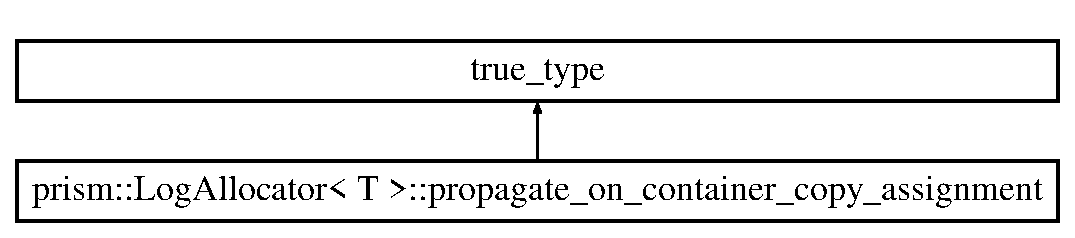
\includegraphics[height=2.000000cm]{structprism_1_1_log_allocator_1_1propagate__on__container__copy__assignment}
\end{center}
\end{figure}


The documentation for this struct was generated from the following file\+:\begin{DoxyCompactItemize}
\item 
inc/prism/h/\hyperlink{_log_allocator_8h}{Log\+Allocator.\+h}\end{DoxyCompactItemize}

\hypertarget{structprism_1_1_log_allocator_1_1propagate__on__container__move__assignment}{}\section{prism\+:\+:Log\+Allocator$<$ T $>$\+:\+:propagate\+\_\+on\+\_\+container\+\_\+move\+\_\+assignment Struct Reference}
\label{structprism_1_1_log_allocator_1_1propagate__on__container__move__assignment}\index{prism\+::\+Log\+Allocator$<$ T $>$\+::propagate\+\_\+on\+\_\+container\+\_\+move\+\_\+assignment@{prism\+::\+Log\+Allocator$<$ T $>$\+::propagate\+\_\+on\+\_\+container\+\_\+move\+\_\+assignment}}
Inheritance diagram for prism\+:\+:Log\+Allocator$<$ T $>$\+:\+:propagate\+\_\+on\+\_\+container\+\_\+move\+\_\+assignment\+:\begin{figure}[H]
\begin{center}
\leavevmode
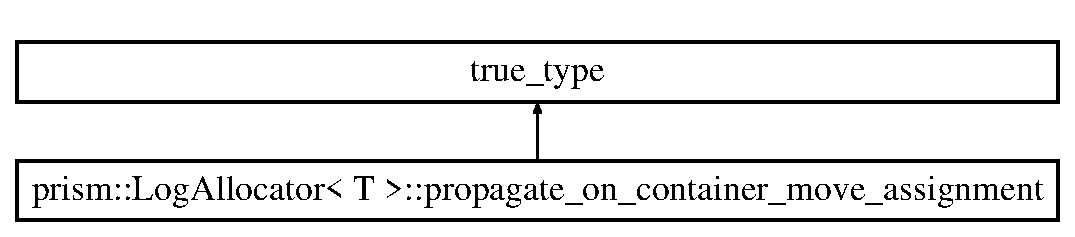
\includegraphics[height=2.000000cm]{structprism_1_1_log_allocator_1_1propagate__on__container__move__assignment}
\end{center}
\end{figure}


The documentation for this struct was generated from the following file\+:\begin{DoxyCompactItemize}
\item 
\hyperlink{_log_allocator_8h}{Log\+Allocator.\+h}\end{DoxyCompactItemize}

\hypertarget{structprism_1_1_log_allocator_1_1propagate__on__container__swap}{}\section{prism\+:\+:Log\+Allocator$<$ T $>$\+:\+:propagate\+\_\+on\+\_\+container\+\_\+swap Struct Reference}
\label{structprism_1_1_log_allocator_1_1propagate__on__container__swap}\index{prism\+::\+Log\+Allocator$<$ T $>$\+::propagate\+\_\+on\+\_\+container\+\_\+swap@{prism\+::\+Log\+Allocator$<$ T $>$\+::propagate\+\_\+on\+\_\+container\+\_\+swap}}
Inheritance diagram for prism\+:\+:Log\+Allocator$<$ T $>$\+:\+:propagate\+\_\+on\+\_\+container\+\_\+swap\+:\begin{figure}[H]
\begin{center}
\leavevmode
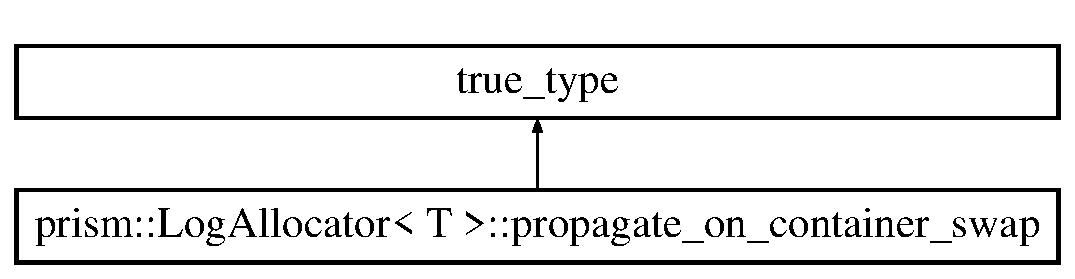
\includegraphics[height=2.000000cm]{structprism_1_1_log_allocator_1_1propagate__on__container__swap}
\end{center}
\end{figure}


The documentation for this struct was generated from the following file\+:\begin{DoxyCompactItemize}
\item 
\hyperlink{_log_allocator_8h}{Log\+Allocator.\+h}\end{DoxyCompactItemize}

\hypertarget{classprism_1_1_quaternion}{}\section{prism\+:\+:Quaternion Class Reference}
\label{classprism_1_1_quaternion}\index{prism\+::\+Quaternion@{prism\+::\+Quaternion}}


{\ttfamily \#include $<$Quaternion.\+h$>$}

\subsection*{Public Member Functions}
\begin{DoxyCompactItemize}
\item 
\hyperlink{classprism_1_1_quaternion_a0d060b8d3623e2add1d269b4e999663d}{Quaternion} (void)
\item 
\hyperlink{classprism_1_1_quaternion_a331e2d14e97aa22f2cce92088ad5594a}{Quaternion} (const float \hyperlink{classprism_1_1_quaternion_aa930b57c8fbba2855722e82080a23cce}{w}, const float \hyperlink{classprism_1_1_quaternion_ab3f80fc41a933a371b2861363997ce22}{x}, const float \hyperlink{classprism_1_1_quaternion_a37023ce86684cb19287ec52cf27072f7}{y}, const float \hyperlink{classprism_1_1_quaternion_a8af7b070028c48f61d1a76b1b49cbaac}{z})
\item 
\hyperlink{classprism_1_1_quaternion_a04c1b60ecb122ea1eaae090a0e98c083}{Quaternion} (const float \hyperlink{classprism_1_1_quaternion_aa930b57c8fbba2855722e82080a23cce}{w}, const \hyperlink{classprism_1_1_vector3}{Vector3} \&v)
\item 
\hyperlink{classprism_1_1_quaternion_af88cd63d0c271ee5e3f7ba74e3349584}{Quaternion} (const \hyperlink{classprism_1_1_quaternion}{Quaternion} \&q)
\item 
virtual \hyperlink{classprism_1_1_quaternion_a1430a69408c646b34a90ea10616599ea}{$\sim$\+Quaternion} (void)
\item 
\hyperlink{classprism_1_1_quaternion}{Quaternion} \hyperlink{classprism_1_1_quaternion_a62430c8b98581769edbc6d339b4ea17b}{conjugate} () const 
\item 
\hyperlink{classprism_1_1_quaternion}{Quaternion} \hyperlink{classprism_1_1_quaternion_add4c30a874ca1d215c299759e4dd9961}{inverse} () const 
\item 
const bool \hyperlink{classprism_1_1_quaternion_a306069da4c274138899739dc30030ffb}{is\+Identity} () const 
\item 
const float \hyperlink{classprism_1_1_quaternion_a3f40222bff891b3320b7934f4e7e72e6}{length} () const 
\item 
const float \hyperlink{classprism_1_1_quaternion_a9b12ad0b7d021d0116e3a2c29a0ecd88}{length\+Squared} () const 
\item 
void \hyperlink{classprism_1_1_quaternion_adce2473719f015c5e8def79cacf4a37c}{normalise} ()
\item 
\hyperlink{classprism_1_1_quaternion}{Quaternion} \hyperlink{classprism_1_1_quaternion_ac9e4890f0614242dbcf2162b23dc483c}{normalised} () const 
\item 
\hyperlink{classprism_1_1_vector3}{Vector3} \hyperlink{classprism_1_1_quaternion_a042b07658410ce868af8ede1cab913b7}{rotated\+Vector} (const \hyperlink{classprism_1_1_vector3}{Vector3} \&v)
\item 
void \hyperlink{classprism_1_1_quaternion_ae639779c2c76874f1d2b3f04aa93f103}{setW} (const float \hyperlink{classprism_1_1_quaternion_aa930b57c8fbba2855722e82080a23cce}{w})
\item 
void \hyperlink{classprism_1_1_quaternion_a66751ee34eab5f4c77e51c018a0001ff}{setX} (const float \hyperlink{classprism_1_1_quaternion_ab3f80fc41a933a371b2861363997ce22}{x})
\item 
void \hyperlink{classprism_1_1_quaternion_ab3db803a8e07017514050bd550ea3e70}{setY} (const float \hyperlink{classprism_1_1_quaternion_a37023ce86684cb19287ec52cf27072f7}{y})
\item 
void \hyperlink{classprism_1_1_quaternion_a92e76b72fd75a6671431f0a2de2a6af2}{setZ} (const float \hyperlink{classprism_1_1_quaternion_a8af7b070028c48f61d1a76b1b49cbaac}{z})
\item 
void \hyperlink{classprism_1_1_quaternion_aabc3e1fd8b643857d206469980b4dff9}{set\+Vector} (const float \hyperlink{classprism_1_1_quaternion_ab3f80fc41a933a371b2861363997ce22}{x}, const float \hyperlink{classprism_1_1_quaternion_a37023ce86684cb19287ec52cf27072f7}{y}, const float \hyperlink{classprism_1_1_quaternion_a8af7b070028c48f61d1a76b1b49cbaac}{z})
\item 
void \hyperlink{classprism_1_1_quaternion_a2a3e3eefffb49c99b6d70d5d299b70e8}{set\+Vector} (const \hyperlink{classprism_1_1_vector3}{Vector3} \&v)
\item 
void \hyperlink{classprism_1_1_quaternion_a008a684b930b6e66f19317696fa47d71}{set\+To\+Identity} ()
\item 
\hyperlink{classprism_1_1_vector3}{Vector3} \hyperlink{classprism_1_1_quaternion_af6ca1a6e1e008c4ad06e2a1306a1edc6}{vector3} () const 
\item 
\hyperlink{classprism_1_1_vector4}{Vector4} \hyperlink{classprism_1_1_quaternion_af0d5601930898339edbfcc2f2d55bb4f}{vector4} () const 
\item 
const float \hyperlink{classprism_1_1_quaternion_aa930b57c8fbba2855722e82080a23cce}{w} () const 
\item 
const float \hyperlink{classprism_1_1_quaternion_ab3f80fc41a933a371b2861363997ce22}{x} () const 
\item 
const float \hyperlink{classprism_1_1_quaternion_a37023ce86684cb19287ec52cf27072f7}{y} () const 
\item 
const float \hyperlink{classprism_1_1_quaternion_a8af7b070028c48f61d1a76b1b49cbaac}{z} () const 
\item 
\hyperlink{classprism_1_1_quaternion}{Quaternion} \& \hyperlink{classprism_1_1_quaternion_a9e99b53a8017eea4d54fba9bb3ff0921}{operator+=} (const \hyperlink{classprism_1_1_quaternion}{Quaternion} \&q)
\item 
\hyperlink{classprism_1_1_quaternion}{Quaternion} \& \hyperlink{classprism_1_1_quaternion_a44b0ad93637f1b7b137850d2b00ce9ae}{operator-\/=} (const \hyperlink{classprism_1_1_quaternion}{Quaternion} \&q)
\item 
\hyperlink{classprism_1_1_quaternion}{Quaternion} \& \hyperlink{classprism_1_1_quaternion_a8e942d7794920c4ee7fcba9abd750c6c}{operator$\ast$=} (const float factor)
\item 
\hyperlink{classprism_1_1_quaternion}{Quaternion} \& \hyperlink{classprism_1_1_quaternion_ab850e8af1efa269eddf42e9171821b52}{operator/=} (const float divisor)
\item 
\hyperlink{classprism_1_1_quaternion}{Quaternion} \& \hyperlink{classprism_1_1_quaternion_a2b53c4088b26aaccc3cbed2496943d23}{operator=} (const \hyperlink{classprism_1_1_quaternion}{Quaternion} \&q)
\end{DoxyCompactItemize}
\subsection*{Static Public Member Functions}
\begin{DoxyCompactItemize}
\item 
static const float \hyperlink{classprism_1_1_quaternion_ad5c802136931b3316185c4bb939555e4}{dot\+Product} (const \hyperlink{classprism_1_1_quaternion}{Quaternion} \&q1, const \hyperlink{classprism_1_1_quaternion}{Quaternion} \&q2)
\item 
static \hyperlink{classprism_1_1_quaternion}{Quaternion} \hyperlink{classprism_1_1_quaternion_aa37e7cababfe0374be478d27a8a8298a}{from\+Axis\+And\+Angle} (const \hyperlink{classprism_1_1_vector3}{Vector3} \&axis, const float angle)
\item 
static \hyperlink{classprism_1_1_quaternion}{Quaternion} \hyperlink{classprism_1_1_quaternion_a35bf3b5687fd42a31c5d33a4b4b65bc0}{from\+Axis\+And\+Angle} (const float x\+Axis, const float y\+Axis, const float z\+Axis, const float angle)
\item 
static \hyperlink{classprism_1_1_quaternion}{Quaternion} \hyperlink{classprism_1_1_quaternion_ab662033392acd76f265f295ba9ddd7db}{identity} ()
\end{DoxyCompactItemize}
\subsection*{Friends}
\begin{DoxyCompactItemize}
\item 
\hyperlink{classprism_1_1_quaternion}{Quaternion} \hyperlink{classprism_1_1_quaternion_a55c89dc55cca66b19679705c566a165a}{operator+} (const \hyperlink{classprism_1_1_quaternion}{Quaternion} \&q1, const \hyperlink{classprism_1_1_quaternion}{Quaternion} \&q2)
\item 
\hyperlink{classprism_1_1_quaternion}{Quaternion} \hyperlink{classprism_1_1_quaternion_a3a5605ba3f0bb654c528d2f7beb34147}{operator-\/} (const \hyperlink{classprism_1_1_quaternion}{Quaternion} \&q1, const \hyperlink{classprism_1_1_quaternion}{Quaternion} \&q2)
\item 
\hyperlink{classprism_1_1_quaternion}{Quaternion} \hyperlink{classprism_1_1_quaternion_a82faed3b53a20e9c2acf7fa2406263c8}{operator-\/} (\hyperlink{classprism_1_1_quaternion}{Quaternion} \&q)
\item 
\hyperlink{classprism_1_1_quaternion}{Quaternion} \hyperlink{classprism_1_1_quaternion_a02f988d3aef50bac26fc6fed8429d6a2}{operator$\ast$} (const \hyperlink{classprism_1_1_quaternion}{Quaternion} \&q1, const \hyperlink{classprism_1_1_quaternion}{Quaternion} \&q2)
\item 
\hyperlink{classprism_1_1_quaternion}{Quaternion} \hyperlink{classprism_1_1_quaternion_a7a69f073f287d3e5e614995aa588dfba}{operator$\ast$} (const \hyperlink{classprism_1_1_quaternion}{Quaternion} \&q, const float factor)
\item 
\hyperlink{classprism_1_1_quaternion}{Quaternion} \hyperlink{classprism_1_1_quaternion_a103d9036740a77394440b39eb4bf3c0b}{operator$\ast$} (const float factor, const \hyperlink{classprism_1_1_quaternion}{Quaternion} \&q)
\item 
\hyperlink{classprism_1_1_quaternion}{Quaternion} \hyperlink{classprism_1_1_quaternion_a3ae869a94a277b595456e7a0d8cf0730}{operator$\ast$} (const \hyperlink{classprism_1_1_quaternion}{Quaternion} \&q, const \hyperlink{classprism_1_1_vector3}{Vector3} \&v)
\item 
\hyperlink{classprism_1_1_quaternion}{Quaternion} \hyperlink{classprism_1_1_quaternion_a9156a92837fec8bf13994dddc21afacf}{operator$\ast$} (const \hyperlink{classprism_1_1_quaternion}{Quaternion} \&q, const \hyperlink{classprism_1_1_vector4}{Vector4} \&v)
\item 
\hyperlink{classprism_1_1_quaternion}{Quaternion} \hyperlink{classprism_1_1_quaternion_a6e207c938a23f83d2bb574d9eb92a56d}{operator/} (const \hyperlink{classprism_1_1_quaternion}{Quaternion} \&q, const float divisor)
\item 
const bool \hyperlink{classprism_1_1_quaternion_a9c72bd1e471ac599aaee1d3dfe729075}{operator==} (const \hyperlink{classprism_1_1_quaternion}{Quaternion} \&q1, const \hyperlink{classprism_1_1_quaternion}{Quaternion} \&q2)
\item 
const bool \hyperlink{classprism_1_1_quaternion_adc2df640ae236b94e01951d891d59e85}{operator!=} (const \hyperlink{classprism_1_1_quaternion}{Quaternion} \&q1, const \hyperlink{classprism_1_1_quaternion}{Quaternion} \&q2)
\item 
std\+::ostream \& \hyperlink{classprism_1_1_quaternion_a9d6837ef4f759aa5ecd417adcea2e908}{operator$<$$<$} (std\+::ostream \&out, const \hyperlink{classprism_1_1_quaternion}{Quaternion} \&q)
\end{DoxyCompactItemize}


\subsection{Constructor \& Destructor Documentation}
\index{prism\+::\+Quaternion@{prism\+::\+Quaternion}!Quaternion@{Quaternion}}
\index{Quaternion@{Quaternion}!prism\+::\+Quaternion@{prism\+::\+Quaternion}}
\subsubsection[{\texorpdfstring{Quaternion(void)}{Quaternion(void)}}]{\setlength{\rightskip}{0pt plus 5cm}prism\+::\+Quaternion\+::\+Quaternion (
\begin{DoxyParamCaption}
\item[{void}]{}
\end{DoxyParamCaption}
)}\hypertarget{classprism_1_1_quaternion_a0d060b8d3623e2add1d269b4e999663d}{}\label{classprism_1_1_quaternion_a0d060b8d3623e2add1d269b4e999663d}
Constructs a quaternion set to the identity state (1,0,0,0). \index{prism\+::\+Quaternion@{prism\+::\+Quaternion}!Quaternion@{Quaternion}}
\index{Quaternion@{Quaternion}!prism\+::\+Quaternion@{prism\+::\+Quaternion}}
\subsubsection[{\texorpdfstring{Quaternion(const float w, const float x, const float y, const float z)}{Quaternion(const float w, const float x, const float y, const float z)}}]{\setlength{\rightskip}{0pt plus 5cm}prism\+::\+Quaternion\+::\+Quaternion (
\begin{DoxyParamCaption}
\item[{const float}]{w, }
\item[{const float}]{x, }
\item[{const float}]{y, }
\item[{const float}]{z}
\end{DoxyParamCaption}
)}\hypertarget{classprism_1_1_quaternion_a331e2d14e97aa22f2cce92088ad5594a}{}\label{classprism_1_1_quaternion_a331e2d14e97aa22f2cce92088ad5594a}
Constructs a quaternion setting the w, x, y and z components to the values passed in. \index{prism\+::\+Quaternion@{prism\+::\+Quaternion}!Quaternion@{Quaternion}}
\index{Quaternion@{Quaternion}!prism\+::\+Quaternion@{prism\+::\+Quaternion}}
\subsubsection[{\texorpdfstring{Quaternion(const float w, const Vector3 \&v)}{Quaternion(const float w, const Vector3 &v)}}]{\setlength{\rightskip}{0pt plus 5cm}prism\+::\+Quaternion\+::\+Quaternion (
\begin{DoxyParamCaption}
\item[{const float}]{w, }
\item[{const {\bf Vector3} \&}]{v}
\end{DoxyParamCaption}
)}\hypertarget{classprism_1_1_quaternion_a04c1b60ecb122ea1eaae090a0e98c083}{}\label{classprism_1_1_quaternion_a04c1b60ecb122ea1eaae090a0e98c083}
Constructs a quaternion from the passed in w and vector. \index{prism\+::\+Quaternion@{prism\+::\+Quaternion}!Quaternion@{Quaternion}}
\index{Quaternion@{Quaternion}!prism\+::\+Quaternion@{prism\+::\+Quaternion}}
\subsubsection[{\texorpdfstring{Quaternion(const Quaternion \&q)}{Quaternion(const Quaternion &q)}}]{\setlength{\rightskip}{0pt plus 5cm}prism\+::\+Quaternion\+::\+Quaternion (
\begin{DoxyParamCaption}
\item[{const {\bf Quaternion} \&}]{q}
\end{DoxyParamCaption}
)}\hypertarget{classprism_1_1_quaternion_af88cd63d0c271ee5e3f7ba74e3349584}{}\label{classprism_1_1_quaternion_af88cd63d0c271ee5e3f7ba74e3349584}
Constructs a quaternion which is a copy of q. \index{prism\+::\+Quaternion@{prism\+::\+Quaternion}!````~Quaternion@{$\sim$\+Quaternion}}
\index{````~Quaternion@{$\sim$\+Quaternion}!prism\+::\+Quaternion@{prism\+::\+Quaternion}}
\subsubsection[{\texorpdfstring{$\sim$\+Quaternion(void)}{~Quaternion(void)}}]{\setlength{\rightskip}{0pt plus 5cm}prism\+::\+Quaternion\+::$\sim$\+Quaternion (
\begin{DoxyParamCaption}
\item[{void}]{}
\end{DoxyParamCaption}
)\hspace{0.3cm}{\ttfamily [virtual]}}\hypertarget{classprism_1_1_quaternion_a1430a69408c646b34a90ea10616599ea}{}\label{classprism_1_1_quaternion_a1430a69408c646b34a90ea10616599ea}


\subsection{Member Function Documentation}
\index{prism\+::\+Quaternion@{prism\+::\+Quaternion}!conjugate@{conjugate}}
\index{conjugate@{conjugate}!prism\+::\+Quaternion@{prism\+::\+Quaternion}}
\subsubsection[{\texorpdfstring{conjugate() const }{conjugate() const }}]{\setlength{\rightskip}{0pt plus 5cm}{\bf Quaternion} prism\+::\+Quaternion\+::conjugate (
\begin{DoxyParamCaption}
{}
\end{DoxyParamCaption}
) const}\hypertarget{classprism_1_1_quaternion_a62430c8b98581769edbc6d339b4ea17b}{}\label{classprism_1_1_quaternion_a62430c8b98581769edbc6d339b4ea17b}
Returns a new \hyperlink{classprism_1_1_quaternion}{Quaternion} which is the result of negating the vector component of this quaternion. This quaternion remains unaltered. Note\+: when a quaternion has been normalised (has unit length of 1) the conjugate and inverse are identical. The quaternion needs to be of unit length in order to perform rotations correctly. \index{prism\+::\+Quaternion@{prism\+::\+Quaternion}!dot\+Product@{dot\+Product}}
\index{dot\+Product@{dot\+Product}!prism\+::\+Quaternion@{prism\+::\+Quaternion}}
\subsubsection[{\texorpdfstring{dot\+Product(const Quaternion \&q1, const Quaternion \&q2)}{dotProduct(const Quaternion &q1, const Quaternion &q2)}}]{\setlength{\rightskip}{0pt plus 5cm}const float prism\+::\+Quaternion\+::dot\+Product (
\begin{DoxyParamCaption}
\item[{const {\bf Quaternion} \&}]{q1, }
\item[{const {\bf Quaternion} \&}]{q2}
\end{DoxyParamCaption}
)\hspace{0.3cm}{\ttfamily [static]}}\hypertarget{classprism_1_1_quaternion_ad5c802136931b3316185c4bb939555e4}{}\label{classprism_1_1_quaternion_ad5c802136931b3316185c4bb939555e4}
Returns a scalar which is the dot product of the two quaternions in the range \mbox{[}-\/1, 1\mbox{]}. The dot product of two quaternions represents the cosine of half of the angle needed to rotate one quaternion into the other. The larger the absolute value the result is (the closer it is to 1) means the closer the two quaternions are in orientation. \index{prism\+::\+Quaternion@{prism\+::\+Quaternion}!from\+Axis\+And\+Angle@{from\+Axis\+And\+Angle}}
\index{from\+Axis\+And\+Angle@{from\+Axis\+And\+Angle}!prism\+::\+Quaternion@{prism\+::\+Quaternion}}
\subsubsection[{\texorpdfstring{from\+Axis\+And\+Angle(const Vector3 \&axis, const float angle)}{fromAxisAndAngle(const Vector3 &axis, const float angle)}}]{\setlength{\rightskip}{0pt plus 5cm}{\bf Quaternion} prism\+::\+Quaternion\+::from\+Axis\+And\+Angle (
\begin{DoxyParamCaption}
\item[{const {\bf Vector3} \&}]{axis, }
\item[{const float}]{angle}
\end{DoxyParamCaption}
)\hspace{0.3cm}{\ttfamily [static]}}\hypertarget{classprism_1_1_quaternion_aa37e7cababfe0374be478d27a8a8298a}{}\label{classprism_1_1_quaternion_aa37e7cababfe0374be478d27a8a8298a}
Returns a normalised quaternion that represents a rotation of angle degrees around the specified axis. If axis is not normalised then this method normalises it. Also, angle is in degrees. \index{prism\+::\+Quaternion@{prism\+::\+Quaternion}!from\+Axis\+And\+Angle@{from\+Axis\+And\+Angle}}
\index{from\+Axis\+And\+Angle@{from\+Axis\+And\+Angle}!prism\+::\+Quaternion@{prism\+::\+Quaternion}}
\subsubsection[{\texorpdfstring{from\+Axis\+And\+Angle(const float x\+Axis, const float y\+Axis, const float z\+Axis, const float angle)}{fromAxisAndAngle(const float xAxis, const float yAxis, const float zAxis, const float angle)}}]{\setlength{\rightskip}{0pt plus 5cm}{\bf Quaternion} prism\+::\+Quaternion\+::from\+Axis\+And\+Angle (
\begin{DoxyParamCaption}
\item[{const float}]{x\+Axis, }
\item[{const float}]{y\+Axis, }
\item[{const float}]{z\+Axis, }
\item[{const float}]{angle}
\end{DoxyParamCaption}
)\hspace{0.3cm}{\ttfamily [static]}}\hypertarget{classprism_1_1_quaternion_a35bf3b5687fd42a31c5d33a4b4b65bc0}{}\label{classprism_1_1_quaternion_a35bf3b5687fd42a31c5d33a4b4b65bc0}
Returns a normalised quaternion that represents a rotation of angle degrees around the specified axis. If the axis specified by x\+Axis, y\+Axis and z\+Axis is not normalised then this method normalises it. Also, angle is in degrees. \index{prism\+::\+Quaternion@{prism\+::\+Quaternion}!identity@{identity}}
\index{identity@{identity}!prism\+::\+Quaternion@{prism\+::\+Quaternion}}
\subsubsection[{\texorpdfstring{identity()}{identity()}}]{\setlength{\rightskip}{0pt plus 5cm}{\bf Quaternion} prism\+::\+Quaternion\+::identity (
\begin{DoxyParamCaption}
{}
\end{DoxyParamCaption}
)\hspace{0.3cm}{\ttfamily [static]}}\hypertarget{classprism_1_1_quaternion_ab662033392acd76f265f295ba9ddd7db}{}\label{classprism_1_1_quaternion_ab662033392acd76f265f295ba9ddd7db}
\index{prism\+::\+Quaternion@{prism\+::\+Quaternion}!inverse@{inverse}}
\index{inverse@{inverse}!prism\+::\+Quaternion@{prism\+::\+Quaternion}}
\subsubsection[{\texorpdfstring{inverse() const }{inverse() const }}]{\setlength{\rightskip}{0pt plus 5cm}{\bf Quaternion} prism\+::\+Quaternion\+::inverse (
\begin{DoxyParamCaption}
{}
\end{DoxyParamCaption}
) const}\hypertarget{classprism_1_1_quaternion_add4c30a874ca1d215c299759e4dd9961}{}\label{classprism_1_1_quaternion_add4c30a874ca1d215c299759e4dd9961}
Returns the inverse of this quaternion. The inverse is defined as dividing the conjugate by the magnitude. Note\+: when a quaternion has been normalised (has unit length of 1) the conjugate and inverse are identical. The quaternion needs to be of unit length in order to perform rotations correctly. \index{prism\+::\+Quaternion@{prism\+::\+Quaternion}!is\+Identity@{is\+Identity}}
\index{is\+Identity@{is\+Identity}!prism\+::\+Quaternion@{prism\+::\+Quaternion}}
\subsubsection[{\texorpdfstring{is\+Identity() const }{isIdentity() const }}]{\setlength{\rightskip}{0pt plus 5cm}const bool prism\+::\+Quaternion\+::is\+Identity (
\begin{DoxyParamCaption}
{}
\end{DoxyParamCaption}
) const}\hypertarget{classprism_1_1_quaternion_a306069da4c274138899739dc30030ffb}{}\label{classprism_1_1_quaternion_a306069da4c274138899739dc30030ffb}
Returns true if w=1 and x=y=z=0, false otherwise. \index{prism\+::\+Quaternion@{prism\+::\+Quaternion}!length@{length}}
\index{length@{length}!prism\+::\+Quaternion@{prism\+::\+Quaternion}}
\subsubsection[{\texorpdfstring{length() const }{length() const }}]{\setlength{\rightskip}{0pt plus 5cm}const float prism\+::\+Quaternion\+::length (
\begin{DoxyParamCaption}
{}
\end{DoxyParamCaption}
) const}\hypertarget{classprism_1_1_quaternion_a3f40222bff891b3320b7934f4e7e72e6}{}\label{classprism_1_1_quaternion_a3f40222bff891b3320b7934f4e7e72e6}
Returns the length (magnitude) of the quaternion. \index{prism\+::\+Quaternion@{prism\+::\+Quaternion}!length\+Squared@{length\+Squared}}
\index{length\+Squared@{length\+Squared}!prism\+::\+Quaternion@{prism\+::\+Quaternion}}
\subsubsection[{\texorpdfstring{length\+Squared() const }{lengthSquared() const }}]{\setlength{\rightskip}{0pt plus 5cm}const float prism\+::\+Quaternion\+::length\+Squared (
\begin{DoxyParamCaption}
{}
\end{DoxyParamCaption}
) const}\hypertarget{classprism_1_1_quaternion_a9b12ad0b7d021d0116e3a2c29a0ecd88}{}\label{classprism_1_1_quaternion_a9b12ad0b7d021d0116e3a2c29a0ecd88}
Returns the squared length of this quaternion. \index{prism\+::\+Quaternion@{prism\+::\+Quaternion}!normalise@{normalise}}
\index{normalise@{normalise}!prism\+::\+Quaternion@{prism\+::\+Quaternion}}
\subsubsection[{\texorpdfstring{normalise()}{normalise()}}]{\setlength{\rightskip}{0pt plus 5cm}void prism\+::\+Quaternion\+::normalise (
\begin{DoxyParamCaption}
{}
\end{DoxyParamCaption}
)}\hypertarget{classprism_1_1_quaternion_adce2473719f015c5e8def79cacf4a37c}{}\label{classprism_1_1_quaternion_adce2473719f015c5e8def79cacf4a37c}
Normalises this quaternion which sets its length to 1. \index{prism\+::\+Quaternion@{prism\+::\+Quaternion}!normalised@{normalised}}
\index{normalised@{normalised}!prism\+::\+Quaternion@{prism\+::\+Quaternion}}
\subsubsection[{\texorpdfstring{normalised() const }{normalised() const }}]{\setlength{\rightskip}{0pt plus 5cm}{\bf Quaternion} prism\+::\+Quaternion\+::normalised (
\begin{DoxyParamCaption}
{}
\end{DoxyParamCaption}
) const}\hypertarget{classprism_1_1_quaternion_ac9e4890f0614242dbcf2162b23dc483c}{}\label{classprism_1_1_quaternion_ac9e4890f0614242dbcf2162b23dc483c}
Returns a copy of this quaternion that has been normalised. \index{prism\+::\+Quaternion@{prism\+::\+Quaternion}!operator$\ast$=@{operator$\ast$=}}
\index{operator$\ast$=@{operator$\ast$=}!prism\+::\+Quaternion@{prism\+::\+Quaternion}}
\subsubsection[{\texorpdfstring{operator$\ast$=(const float factor)}{operator*=(const float factor)}}]{\setlength{\rightskip}{0pt plus 5cm}{\bf Quaternion} \& prism\+::\+Quaternion\+::operator$\ast$= (
\begin{DoxyParamCaption}
\item[{const float}]{factor}
\end{DoxyParamCaption}
)}\hypertarget{classprism_1_1_quaternion_a8e942d7794920c4ee7fcba9abd750c6c}{}\label{classprism_1_1_quaternion_a8e942d7794920c4ee7fcba9abd750c6c}
Returns a reference to this \hyperlink{classprism_1_1_quaternion}{Quaternion} which has had each component multiplied by factor. \index{prism\+::\+Quaternion@{prism\+::\+Quaternion}!operator+=@{operator+=}}
\index{operator+=@{operator+=}!prism\+::\+Quaternion@{prism\+::\+Quaternion}}
\subsubsection[{\texorpdfstring{operator+=(const Quaternion \&q)}{operator+=(const Quaternion &q)}}]{\setlength{\rightskip}{0pt plus 5cm}{\bf Quaternion} \& prism\+::\+Quaternion\+::operator+= (
\begin{DoxyParamCaption}
\item[{const {\bf Quaternion} \&}]{q}
\end{DoxyParamCaption}
)}\hypertarget{classprism_1_1_quaternion_a9e99b53a8017eea4d54fba9bb3ff0921}{}\label{classprism_1_1_quaternion_a9e99b53a8017eea4d54fba9bb3ff0921}
Returns a reference to this \hyperlink{classprism_1_1_quaternion}{Quaternion} which has had q added to it. \index{prism\+::\+Quaternion@{prism\+::\+Quaternion}!operator-\/=@{operator-\/=}}
\index{operator-\/=@{operator-\/=}!prism\+::\+Quaternion@{prism\+::\+Quaternion}}
\subsubsection[{\texorpdfstring{operator-\/=(const Quaternion \&q)}{operator-=(const Quaternion &q)}}]{\setlength{\rightskip}{0pt plus 5cm}{\bf Quaternion} \& prism\+::\+Quaternion\+::operator-\/= (
\begin{DoxyParamCaption}
\item[{const {\bf Quaternion} \&}]{q}
\end{DoxyParamCaption}
)}\hypertarget{classprism_1_1_quaternion_a44b0ad93637f1b7b137850d2b00ce9ae}{}\label{classprism_1_1_quaternion_a44b0ad93637f1b7b137850d2b00ce9ae}
Returns a reference to this \hyperlink{classprism_1_1_quaternion}{Quaternion} which has had q subtracted from it. \index{prism\+::\+Quaternion@{prism\+::\+Quaternion}!operator/=@{operator/=}}
\index{operator/=@{operator/=}!prism\+::\+Quaternion@{prism\+::\+Quaternion}}
\subsubsection[{\texorpdfstring{operator/=(const float divisor)}{operator/=(const float divisor)}}]{\setlength{\rightskip}{0pt plus 5cm}{\bf Quaternion} \& prism\+::\+Quaternion\+::operator/= (
\begin{DoxyParamCaption}
\item[{const float}]{divisor}
\end{DoxyParamCaption}
)}\hypertarget{classprism_1_1_quaternion_ab850e8af1efa269eddf42e9171821b52}{}\label{classprism_1_1_quaternion_ab850e8af1efa269eddf42e9171821b52}
Returns a reference to this \hyperlink{classprism_1_1_quaternion}{Quaternion} which has had each component divided by divisor. If divisor is 0 then nothing happens. \index{prism\+::\+Quaternion@{prism\+::\+Quaternion}!operator=@{operator=}}
\index{operator=@{operator=}!prism\+::\+Quaternion@{prism\+::\+Quaternion}}
\subsubsection[{\texorpdfstring{operator=(const Quaternion \&q)}{operator=(const Quaternion &q)}}]{\setlength{\rightskip}{0pt plus 5cm}{\bf Quaternion} \& prism\+::\+Quaternion\+::operator= (
\begin{DoxyParamCaption}
\item[{const {\bf Quaternion} \&}]{q}
\end{DoxyParamCaption}
)}\hypertarget{classprism_1_1_quaternion_a2b53c4088b26aaccc3cbed2496943d23}{}\label{classprism_1_1_quaternion_a2b53c4088b26aaccc3cbed2496943d23}
Assignment operator assigns the component values of q to this quaternion. \index{prism\+::\+Quaternion@{prism\+::\+Quaternion}!rotated\+Vector@{rotated\+Vector}}
\index{rotated\+Vector@{rotated\+Vector}!prism\+::\+Quaternion@{prism\+::\+Quaternion}}
\subsubsection[{\texorpdfstring{rotated\+Vector(const Vector3 \&v)}{rotatedVector(const Vector3 &v)}}]{\setlength{\rightskip}{0pt plus 5cm}{\bf Vector3} prism\+::\+Quaternion\+::rotated\+Vector (
\begin{DoxyParamCaption}
\item[{const {\bf Vector3} \&}]{v}
\end{DoxyParamCaption}
)}\hypertarget{classprism_1_1_quaternion_a042b07658410ce868af8ede1cab913b7}{}\label{classprism_1_1_quaternion_a042b07658410ce868af8ede1cab913b7}
Rotates vector v with this quaternion and returns a new \hyperlink{classprism_1_1_vector3}{Vector3} with the result. \index{prism\+::\+Quaternion@{prism\+::\+Quaternion}!set\+To\+Identity@{set\+To\+Identity}}
\index{set\+To\+Identity@{set\+To\+Identity}!prism\+::\+Quaternion@{prism\+::\+Quaternion}}
\subsubsection[{\texorpdfstring{set\+To\+Identity()}{setToIdentity()}}]{\setlength{\rightskip}{0pt plus 5cm}void prism\+::\+Quaternion\+::set\+To\+Identity (
\begin{DoxyParamCaption}
{}
\end{DoxyParamCaption}
)}\hypertarget{classprism_1_1_quaternion_a008a684b930b6e66f19317696fa47d71}{}\label{classprism_1_1_quaternion_a008a684b930b6e66f19317696fa47d71}
Sets the quaternion to its identity state which sets w=1 and x=y=z=0 i.\+e. zero vector \index{prism\+::\+Quaternion@{prism\+::\+Quaternion}!set\+Vector@{set\+Vector}}
\index{set\+Vector@{set\+Vector}!prism\+::\+Quaternion@{prism\+::\+Quaternion}}
\subsubsection[{\texorpdfstring{set\+Vector(const float x, const float y, const float z)}{setVector(const float x, const float y, const float z)}}]{\setlength{\rightskip}{0pt plus 5cm}void prism\+::\+Quaternion\+::set\+Vector (
\begin{DoxyParamCaption}
\item[{const float}]{x, }
\item[{const float}]{y, }
\item[{const float}]{z}
\end{DoxyParamCaption}
)}\hypertarget{classprism_1_1_quaternion_aabc3e1fd8b643857d206469980b4dff9}{}\label{classprism_1_1_quaternion_aabc3e1fd8b643857d206469980b4dff9}
Sets the vector component of this quaternion to the values passed in. \index{prism\+::\+Quaternion@{prism\+::\+Quaternion}!set\+Vector@{set\+Vector}}
\index{set\+Vector@{set\+Vector}!prism\+::\+Quaternion@{prism\+::\+Quaternion}}
\subsubsection[{\texorpdfstring{set\+Vector(const Vector3 \&v)}{setVector(const Vector3 &v)}}]{\setlength{\rightskip}{0pt plus 5cm}void prism\+::\+Quaternion\+::set\+Vector (
\begin{DoxyParamCaption}
\item[{const {\bf Vector3} \&}]{v}
\end{DoxyParamCaption}
)}\hypertarget{classprism_1_1_quaternion_a2a3e3eefffb49c99b6d70d5d299b70e8}{}\label{classprism_1_1_quaternion_a2a3e3eefffb49c99b6d70d5d299b70e8}
Sets the vector component of this quaternion to the specified vector passed in. \index{prism\+::\+Quaternion@{prism\+::\+Quaternion}!setW@{setW}}
\index{setW@{setW}!prism\+::\+Quaternion@{prism\+::\+Quaternion}}
\subsubsection[{\texorpdfstring{set\+W(const float w)}{setW(const float w)}}]{\setlength{\rightskip}{0pt plus 5cm}void prism\+::\+Quaternion\+::setW (
\begin{DoxyParamCaption}
\item[{const float}]{w}
\end{DoxyParamCaption}
)}\hypertarget{classprism_1_1_quaternion_ae639779c2c76874f1d2b3f04aa93f103}{}\label{classprism_1_1_quaternion_ae639779c2c76874f1d2b3f04aa93f103}
Sets the w component of this quaternion. \index{prism\+::\+Quaternion@{prism\+::\+Quaternion}!setX@{setX}}
\index{setX@{setX}!prism\+::\+Quaternion@{prism\+::\+Quaternion}}
\subsubsection[{\texorpdfstring{set\+X(const float x)}{setX(const float x)}}]{\setlength{\rightskip}{0pt plus 5cm}void prism\+::\+Quaternion\+::setX (
\begin{DoxyParamCaption}
\item[{const float}]{x}
\end{DoxyParamCaption}
)}\hypertarget{classprism_1_1_quaternion_a66751ee34eab5f4c77e51c018a0001ff}{}\label{classprism_1_1_quaternion_a66751ee34eab5f4c77e51c018a0001ff}
Sets the x component of this quaternion. \index{prism\+::\+Quaternion@{prism\+::\+Quaternion}!setY@{setY}}
\index{setY@{setY}!prism\+::\+Quaternion@{prism\+::\+Quaternion}}
\subsubsection[{\texorpdfstring{set\+Y(const float y)}{setY(const float y)}}]{\setlength{\rightskip}{0pt plus 5cm}void prism\+::\+Quaternion\+::setY (
\begin{DoxyParamCaption}
\item[{const float}]{y}
\end{DoxyParamCaption}
)}\hypertarget{classprism_1_1_quaternion_ab3db803a8e07017514050bd550ea3e70}{}\label{classprism_1_1_quaternion_ab3db803a8e07017514050bd550ea3e70}
Sets the y component of this quaternion. \index{prism\+::\+Quaternion@{prism\+::\+Quaternion}!setZ@{setZ}}
\index{setZ@{setZ}!prism\+::\+Quaternion@{prism\+::\+Quaternion}}
\subsubsection[{\texorpdfstring{set\+Z(const float z)}{setZ(const float z)}}]{\setlength{\rightskip}{0pt plus 5cm}void prism\+::\+Quaternion\+::setZ (
\begin{DoxyParamCaption}
\item[{const float}]{z}
\end{DoxyParamCaption}
)}\hypertarget{classprism_1_1_quaternion_a92e76b72fd75a6671431f0a2de2a6af2}{}\label{classprism_1_1_quaternion_a92e76b72fd75a6671431f0a2de2a6af2}
Sets the z component of this quaternion. \index{prism\+::\+Quaternion@{prism\+::\+Quaternion}!vector3@{vector3}}
\index{vector3@{vector3}!prism\+::\+Quaternion@{prism\+::\+Quaternion}}
\subsubsection[{\texorpdfstring{vector3() const }{vector3() const }}]{\setlength{\rightskip}{0pt plus 5cm}{\bf Vector3} prism\+::\+Quaternion\+::vector3 (
\begin{DoxyParamCaption}
{}
\end{DoxyParamCaption}
) const}\hypertarget{classprism_1_1_quaternion_af6ca1a6e1e008c4ad06e2a1306a1edc6}{}\label{classprism_1_1_quaternion_af6ca1a6e1e008c4ad06e2a1306a1edc6}
Returns a \hyperlink{classprism_1_1_vector3}{Vector3} which is the vector component of this quaternion i.\+e. x, y and z \index{prism\+::\+Quaternion@{prism\+::\+Quaternion}!vector4@{vector4}}
\index{vector4@{vector4}!prism\+::\+Quaternion@{prism\+::\+Quaternion}}
\subsubsection[{\texorpdfstring{vector4() const }{vector4() const }}]{\setlength{\rightskip}{0pt plus 5cm}{\bf Vector4} prism\+::\+Quaternion\+::vector4 (
\begin{DoxyParamCaption}
{}
\end{DoxyParamCaption}
) const}\hypertarget{classprism_1_1_quaternion_af0d5601930898339edbfcc2f2d55bb4f}{}\label{classprism_1_1_quaternion_af0d5601930898339edbfcc2f2d55bb4f}
Returns a \hyperlink{classprism_1_1_vector4}{Vector4} which is the vector component of this quaternion, i.\+e. x, y and z, additionally with the w component set to 1. \index{prism\+::\+Quaternion@{prism\+::\+Quaternion}!w@{w}}
\index{w@{w}!prism\+::\+Quaternion@{prism\+::\+Quaternion}}
\subsubsection[{\texorpdfstring{w() const }{w() const }}]{\setlength{\rightskip}{0pt plus 5cm}const float prism\+::\+Quaternion\+::w (
\begin{DoxyParamCaption}
{}
\end{DoxyParamCaption}
) const}\hypertarget{classprism_1_1_quaternion_aa930b57c8fbba2855722e82080a23cce}{}\label{classprism_1_1_quaternion_aa930b57c8fbba2855722e82080a23cce}
Returns the w component of this quaternion. \index{prism\+::\+Quaternion@{prism\+::\+Quaternion}!x@{x}}
\index{x@{x}!prism\+::\+Quaternion@{prism\+::\+Quaternion}}
\subsubsection[{\texorpdfstring{x() const }{x() const }}]{\setlength{\rightskip}{0pt plus 5cm}const float prism\+::\+Quaternion\+::x (
\begin{DoxyParamCaption}
{}
\end{DoxyParamCaption}
) const}\hypertarget{classprism_1_1_quaternion_ab3f80fc41a933a371b2861363997ce22}{}\label{classprism_1_1_quaternion_ab3f80fc41a933a371b2861363997ce22}
Returns the x component of this quaternion. \index{prism\+::\+Quaternion@{prism\+::\+Quaternion}!y@{y}}
\index{y@{y}!prism\+::\+Quaternion@{prism\+::\+Quaternion}}
\subsubsection[{\texorpdfstring{y() const }{y() const }}]{\setlength{\rightskip}{0pt plus 5cm}const float prism\+::\+Quaternion\+::y (
\begin{DoxyParamCaption}
{}
\end{DoxyParamCaption}
) const}\hypertarget{classprism_1_1_quaternion_a37023ce86684cb19287ec52cf27072f7}{}\label{classprism_1_1_quaternion_a37023ce86684cb19287ec52cf27072f7}
Returns the y component of this quaternion. \index{prism\+::\+Quaternion@{prism\+::\+Quaternion}!z@{z}}
\index{z@{z}!prism\+::\+Quaternion@{prism\+::\+Quaternion}}
\subsubsection[{\texorpdfstring{z() const }{z() const }}]{\setlength{\rightskip}{0pt plus 5cm}const float prism\+::\+Quaternion\+::z (
\begin{DoxyParamCaption}
{}
\end{DoxyParamCaption}
) const}\hypertarget{classprism_1_1_quaternion_a8af7b070028c48f61d1a76b1b49cbaac}{}\label{classprism_1_1_quaternion_a8af7b070028c48f61d1a76b1b49cbaac}
Returns the z component of this quaternion. 

\subsection{Friends And Related Function Documentation}
\index{prism\+::\+Quaternion@{prism\+::\+Quaternion}!operator"!=@{operator"!=}}
\index{operator"!=@{operator"!=}!prism\+::\+Quaternion@{prism\+::\+Quaternion}}
\subsubsection[{\texorpdfstring{operator"!=}{operator!=}}]{\setlength{\rightskip}{0pt plus 5cm}const bool operator!= (
\begin{DoxyParamCaption}
\item[{const {\bf Quaternion} \&}]{q1, }
\item[{const {\bf Quaternion} \&}]{q2}
\end{DoxyParamCaption}
)\hspace{0.3cm}{\ttfamily [friend]}}\hypertarget{classprism_1_1_quaternion_adc2df640ae236b94e01951d891d59e85}{}\label{classprism_1_1_quaternion_adc2df640ae236b94e01951d891d59e85}
Compares q1 and q2 and returns true if they are not equal, false otherwise. \index{prism\+::\+Quaternion@{prism\+::\+Quaternion}!operator$\ast$@{operator$\ast$}}
\index{operator$\ast$@{operator$\ast$}!prism\+::\+Quaternion@{prism\+::\+Quaternion}}
\subsubsection[{\texorpdfstring{operator$\ast$}{operator*}}]{\setlength{\rightskip}{0pt plus 5cm}{\bf Quaternion} operator$\ast$ (
\begin{DoxyParamCaption}
\item[{const {\bf Quaternion} \&}]{q1, }
\item[{const {\bf Quaternion} \&}]{q2}
\end{DoxyParamCaption}
)\hspace{0.3cm}{\ttfamily [friend]}}\hypertarget{classprism_1_1_quaternion_a02f988d3aef50bac26fc6fed8429d6a2}{}\label{classprism_1_1_quaternion_a02f988d3aef50bac26fc6fed8429d6a2}
Returns a \hyperlink{classprism_1_1_quaternion}{Quaternion} that is the product of q1 and q2. Note\+: quaternion multiplication is associative so a(bc) = (ab)c but is not commutitive so q1q2 does not always equal q2q1. Order matters! \index{prism\+::\+Quaternion@{prism\+::\+Quaternion}!operator$\ast$@{operator$\ast$}}
\index{operator$\ast$@{operator$\ast$}!prism\+::\+Quaternion@{prism\+::\+Quaternion}}
\subsubsection[{\texorpdfstring{operator$\ast$}{operator*}}]{\setlength{\rightskip}{0pt plus 5cm}{\bf Quaternion} operator$\ast$ (
\begin{DoxyParamCaption}
\item[{const {\bf Quaternion} \&}]{q, }
\item[{const float}]{factor}
\end{DoxyParamCaption}
)\hspace{0.3cm}{\ttfamily [friend]}}\hypertarget{classprism_1_1_quaternion_a7a69f073f287d3e5e614995aa588dfba}{}\label{classprism_1_1_quaternion_a7a69f073f287d3e5e614995aa588dfba}
Returns a \hyperlink{classprism_1_1_quaternion}{Quaternion} that is the result of multiplying each component of q by factor. \index{prism\+::\+Quaternion@{prism\+::\+Quaternion}!operator$\ast$@{operator$\ast$}}
\index{operator$\ast$@{operator$\ast$}!prism\+::\+Quaternion@{prism\+::\+Quaternion}}
\subsubsection[{\texorpdfstring{operator$\ast$}{operator*}}]{\setlength{\rightskip}{0pt plus 5cm}{\bf Quaternion} operator$\ast$ (
\begin{DoxyParamCaption}
\item[{const float}]{factor, }
\item[{const {\bf Quaternion} \&}]{q}
\end{DoxyParamCaption}
)\hspace{0.3cm}{\ttfamily [friend]}}\hypertarget{classprism_1_1_quaternion_a103d9036740a77394440b39eb4bf3c0b}{}\label{classprism_1_1_quaternion_a103d9036740a77394440b39eb4bf3c0b}
Returns a \hyperlink{classprism_1_1_quaternion}{Quaternion} that is the result of multiplying each component of q by factor. \index{prism\+::\+Quaternion@{prism\+::\+Quaternion}!operator$\ast$@{operator$\ast$}}
\index{operator$\ast$@{operator$\ast$}!prism\+::\+Quaternion@{prism\+::\+Quaternion}}
\subsubsection[{\texorpdfstring{operator$\ast$}{operator*}}]{\setlength{\rightskip}{0pt plus 5cm}{\bf Quaternion} operator$\ast$ (
\begin{DoxyParamCaption}
\item[{const {\bf Quaternion} \&}]{q, }
\item[{const {\bf Vector3} \&}]{v}
\end{DoxyParamCaption}
)\hspace{0.3cm}{\ttfamily [friend]}}\hypertarget{classprism_1_1_quaternion_a3ae869a94a277b595456e7a0d8cf0730}{}\label{classprism_1_1_quaternion_a3ae869a94a277b595456e7a0d8cf0730}
Multiplies a quaternion and vector3 together and returns a quaternion as a result. The vector is just transformed into a quaternion (setting w = 0) and then the two quaternions are multiplied. \index{prism\+::\+Quaternion@{prism\+::\+Quaternion}!operator$\ast$@{operator$\ast$}}
\index{operator$\ast$@{operator$\ast$}!prism\+::\+Quaternion@{prism\+::\+Quaternion}}
\subsubsection[{\texorpdfstring{operator$\ast$}{operator*}}]{\setlength{\rightskip}{0pt plus 5cm}{\bf Quaternion} operator$\ast$ (
\begin{DoxyParamCaption}
\item[{const {\bf Quaternion} \&}]{q, }
\item[{const {\bf Vector4} \&}]{v}
\end{DoxyParamCaption}
)\hspace{0.3cm}{\ttfamily [friend]}}\hypertarget{classprism_1_1_quaternion_a9156a92837fec8bf13994dddc21afacf}{}\label{classprism_1_1_quaternion_a9156a92837fec8bf13994dddc21afacf}
Multiplies a quaternion and \hyperlink{classprism_1_1_vector4}{Vector4} together and returns a quaternion as a result. The vector is just transformed into a quaternion and then the two quaternions are multiplied. \index{prism\+::\+Quaternion@{prism\+::\+Quaternion}!operator+@{operator+}}
\index{operator+@{operator+}!prism\+::\+Quaternion@{prism\+::\+Quaternion}}
\subsubsection[{\texorpdfstring{operator+}{operator+}}]{\setlength{\rightskip}{0pt plus 5cm}{\bf Quaternion} operator+ (
\begin{DoxyParamCaption}
\item[{const {\bf Quaternion} \&}]{q1, }
\item[{const {\bf Quaternion} \&}]{q2}
\end{DoxyParamCaption}
)\hspace{0.3cm}{\ttfamily [friend]}}\hypertarget{classprism_1_1_quaternion_a55c89dc55cca66b19679705c566a165a}{}\label{classprism_1_1_quaternion_a55c89dc55cca66b19679705c566a165a}
Returns a \hyperlink{classprism_1_1_quaternion}{Quaternion} that is the sum of q1 and q2 i.\+e. each component of q1 is added to the corresponding component of q2. \index{prism\+::\+Quaternion@{prism\+::\+Quaternion}!operator-\/@{operator-\/}}
\index{operator-\/@{operator-\/}!prism\+::\+Quaternion@{prism\+::\+Quaternion}}
\subsubsection[{\texorpdfstring{operator-\/}{operator-}}]{\setlength{\rightskip}{0pt plus 5cm}{\bf Quaternion} operator-\/ (
\begin{DoxyParamCaption}
\item[{const {\bf Quaternion} \&}]{q1, }
\item[{const {\bf Quaternion} \&}]{q2}
\end{DoxyParamCaption}
)\hspace{0.3cm}{\ttfamily [friend]}}\hypertarget{classprism_1_1_quaternion_a3a5605ba3f0bb654c528d2f7beb34147}{}\label{classprism_1_1_quaternion_a3a5605ba3f0bb654c528d2f7beb34147}
Returns a \hyperlink{classprism_1_1_quaternion}{Quaternion} that is the result of subtracting q2 from q1 i.\+e. each component of q2 is subtracted from the corresponding component of q1. \index{prism\+::\+Quaternion@{prism\+::\+Quaternion}!operator-\/@{operator-\/}}
\index{operator-\/@{operator-\/}!prism\+::\+Quaternion@{prism\+::\+Quaternion}}
\subsubsection[{\texorpdfstring{operator-\/}{operator-}}]{\setlength{\rightskip}{0pt plus 5cm}{\bf Quaternion} operator-\/ (
\begin{DoxyParamCaption}
\item[{{\bf Quaternion} \&}]{q}
\end{DoxyParamCaption}
)\hspace{0.3cm}{\ttfamily [friend]}}\hypertarget{classprism_1_1_quaternion_a82faed3b53a20e9c2acf7fa2406263c8}{}\label{classprism_1_1_quaternion_a82faed3b53a20e9c2acf7fa2406263c8}
Returns a \hyperlink{classprism_1_1_quaternion}{Quaternion} which has had each component of q negated. \index{prism\+::\+Quaternion@{prism\+::\+Quaternion}!operator/@{operator/}}
\index{operator/@{operator/}!prism\+::\+Quaternion@{prism\+::\+Quaternion}}
\subsubsection[{\texorpdfstring{operator/}{operator/}}]{\setlength{\rightskip}{0pt plus 5cm}{\bf Quaternion} operator/ (
\begin{DoxyParamCaption}
\item[{const {\bf Quaternion} \&}]{q, }
\item[{const float}]{divisor}
\end{DoxyParamCaption}
)\hspace{0.3cm}{\ttfamily [friend]}}\hypertarget{classprism_1_1_quaternion_a6e207c938a23f83d2bb574d9eb92a56d}{}\label{classprism_1_1_quaternion_a6e207c938a23f83d2bb574d9eb92a56d}
Returns a \hyperlink{classprism_1_1_quaternion}{Quaternion} that is the result of dividing each component of q by divisor. If divisor is 0 then a identity quaternion is returned instead. \index{prism\+::\+Quaternion@{prism\+::\+Quaternion}!operator$<$$<$@{operator$<$$<$}}
\index{operator$<$$<$@{operator$<$$<$}!prism\+::\+Quaternion@{prism\+::\+Quaternion}}
\subsubsection[{\texorpdfstring{operator$<$$<$}{operator<<}}]{\setlength{\rightskip}{0pt plus 5cm}std\+::ostream\& operator$<$$<$ (
\begin{DoxyParamCaption}
\item[{std\+::ostream \&}]{out, }
\item[{const {\bf Quaternion} \&}]{q}
\end{DoxyParamCaption}
)\hspace{0.3cm}{\ttfamily [friend]}}\hypertarget{classprism_1_1_quaternion_a9d6837ef4f759aa5ecd417adcea2e908}{}\label{classprism_1_1_quaternion_a9d6837ef4f759aa5ecd417adcea2e908}
Returns a reference to a stream which allows an instance of \hyperlink{classprism_1_1_quaternion}{Quaternion} to be written to the stream. \index{prism\+::\+Quaternion@{prism\+::\+Quaternion}!operator==@{operator==}}
\index{operator==@{operator==}!prism\+::\+Quaternion@{prism\+::\+Quaternion}}
\subsubsection[{\texorpdfstring{operator==}{operator==}}]{\setlength{\rightskip}{0pt plus 5cm}const bool operator== (
\begin{DoxyParamCaption}
\item[{const {\bf Quaternion} \&}]{q1, }
\item[{const {\bf Quaternion} \&}]{q2}
\end{DoxyParamCaption}
)\hspace{0.3cm}{\ttfamily [friend]}}\hypertarget{classprism_1_1_quaternion_a9c72bd1e471ac599aaee1d3dfe729075}{}\label{classprism_1_1_quaternion_a9c72bd1e471ac599aaee1d3dfe729075}
Compares q1 and q2 and returns true if they are equal, false otherwise. 

The documentation for this class was generated from the following files\+:\begin{DoxyCompactItemize}
\item 
inc/prism/geometry/\hyperlink{_quaternion_8h}{Quaternion.\+h}\item 
src/prism/geometry/\hyperlink{_quaternion_8cpp}{Quaternion.\+cpp}\end{DoxyCompactItemize}

\hypertarget{classprism_1_1_queue}{}\section{prism\+:\+:Queue$<$ T, Container\+Type $>$ Class Template Reference}
\label{classprism_1_1_queue}\index{prism\+::\+Queue$<$ T, Container\+Type $>$@{prism\+::\+Queue$<$ T, Container\+Type $>$}}


{\ttfamily \#include $<$Queue.\+h$>$}

\subsection*{Public Member Functions}
\begin{DoxyCompactItemize}
\item 
\hyperlink{classprism_1_1_queue_a943cba3a4cde79f5fa364007f95f7f0a}{Queue} ()
\item 
T \& \hyperlink{classprism_1_1_queue_aec36e33bfdca9864e6d306858aae280d}{back} ()
\item 
const T \& \hyperlink{classprism_1_1_queue_affa363ef43576ea8cafe181044ffa608}{back} () const 
\item 
T \hyperlink{classprism_1_1_queue_a94b089c9e56c3dee7628c8c63ee9cc5f}{dequeue} ()
\item 
void \hyperlink{classprism_1_1_queue_a36e39d3d29bc77408b365d9652ce4b61}{enqueue} (const T \&value)
\item 
T \& \hyperlink{classprism_1_1_queue_a5dc211a8c79d1d089a678ebc7f2e43c4}{front} ()
\item 
const T \& \hyperlink{classprism_1_1_queue_a22bd93b06bacca633756a149ba27bb06}{front} () const 
\item 
const bool \hyperlink{classprism_1_1_queue_a0d747caa114058aceceb3bb789500ee4}{is\+Empty} () const 
\item 
T \hyperlink{classprism_1_1_queue_ac5a988d20ed06a55cb37d62d37e0ceda}{pop} ()
\item 
void \hyperlink{classprism_1_1_queue_af5cb19bac94390121914beb4ad147405}{push} (const T \&value)
\item 
const int \hyperlink{classprism_1_1_queue_a1c868feb72c566af4756593f2b5747d9}{size} () const 
\end{DoxyCompactItemize}


\subsection{Constructor \& Destructor Documentation}
\index{prism\+::\+Queue@{prism\+::\+Queue}!Queue@{Queue}}
\index{Queue@{Queue}!prism\+::\+Queue@{prism\+::\+Queue}}
\subsubsection[{\texorpdfstring{Queue()}{Queue()}}]{\setlength{\rightskip}{0pt plus 5cm}template$<$class T , class Container\+Type $>$ {\bf prism\+::\+Queue}$<$ T, Container\+Type $>$\+::{\bf Queue} (
\begin{DoxyParamCaption}
{}
\end{DoxyParamCaption}
)}\hypertarget{classprism_1_1_queue_a943cba3a4cde79f5fa364007f95f7f0a}{}\label{classprism_1_1_queue_a943cba3a4cde79f5fa364007f95f7f0a}
Creates an empty queue. 

\subsection{Member Function Documentation}
\index{prism\+::\+Queue@{prism\+::\+Queue}!back@{back}}
\index{back@{back}!prism\+::\+Queue@{prism\+::\+Queue}}
\subsubsection[{\texorpdfstring{back()}{back()}}]{\setlength{\rightskip}{0pt plus 5cm}template$<$class T , class Container\+Type $>$ T \& {\bf prism\+::\+Queue}$<$ T, Container\+Type $>$\+::back (
\begin{DoxyParamCaption}
{}
\end{DoxyParamCaption}
)}\hypertarget{classprism_1_1_queue_aec36e33bfdca9864e6d306858aae280d}{}\label{classprism_1_1_queue_aec36e33bfdca9864e6d306858aae280d}
Returns a reference to the last item in the queue. \index{prism\+::\+Queue@{prism\+::\+Queue}!back@{back}}
\index{back@{back}!prism\+::\+Queue@{prism\+::\+Queue}}
\subsubsection[{\texorpdfstring{back() const }{back() const }}]{\setlength{\rightskip}{0pt plus 5cm}template$<$class T , class Container\+Type $>$ const T \& {\bf prism\+::\+Queue}$<$ T, Container\+Type $>$\+::back (
\begin{DoxyParamCaption}
{}
\end{DoxyParamCaption}
) const}\hypertarget{classprism_1_1_queue_affa363ef43576ea8cafe181044ffa608}{}\label{classprism_1_1_queue_affa363ef43576ea8cafe181044ffa608}
Returns a const reference to the last item in the queue. \index{prism\+::\+Queue@{prism\+::\+Queue}!dequeue@{dequeue}}
\index{dequeue@{dequeue}!prism\+::\+Queue@{prism\+::\+Queue}}
\subsubsection[{\texorpdfstring{dequeue()}{dequeue()}}]{\setlength{\rightskip}{0pt plus 5cm}template$<$class T , class Container\+Type $>$ T {\bf prism\+::\+Queue}$<$ T, Container\+Type $>$\+::dequeue (
\begin{DoxyParamCaption}
{}
\end{DoxyParamCaption}
)}\hypertarget{classprism_1_1_queue_a94b089c9e56c3dee7628c8c63ee9cc5f}{}\label{classprism_1_1_queue_a94b089c9e56c3dee7628c8c63ee9cc5f}
Removes and returns the item at the front of the queue. \index{prism\+::\+Queue@{prism\+::\+Queue}!enqueue@{enqueue}}
\index{enqueue@{enqueue}!prism\+::\+Queue@{prism\+::\+Queue}}
\subsubsection[{\texorpdfstring{enqueue(const T \&value)}{enqueue(const T &value)}}]{\setlength{\rightskip}{0pt plus 5cm}template$<$class T , class Container\+Type $>$ void {\bf prism\+::\+Queue}$<$ T, Container\+Type $>$\+::enqueue (
\begin{DoxyParamCaption}
\item[{const T \&}]{value}
\end{DoxyParamCaption}
)}\hypertarget{classprism_1_1_queue_a36e39d3d29bc77408b365d9652ce4b61}{}\label{classprism_1_1_queue_a36e39d3d29bc77408b365d9652ce4b61}
Adds {\itshape value} at the end of the queue. \index{prism\+::\+Queue@{prism\+::\+Queue}!front@{front}}
\index{front@{front}!prism\+::\+Queue@{prism\+::\+Queue}}
\subsubsection[{\texorpdfstring{front()}{front()}}]{\setlength{\rightskip}{0pt plus 5cm}template$<$class T , class Container\+Type $>$ T \& {\bf prism\+::\+Queue}$<$ T, Container\+Type $>$\+::front (
\begin{DoxyParamCaption}
{}
\end{DoxyParamCaption}
)}\hypertarget{classprism_1_1_queue_a5dc211a8c79d1d089a678ebc7f2e43c4}{}\label{classprism_1_1_queue_a5dc211a8c79d1d089a678ebc7f2e43c4}
Returns a reference to the item at the front of the queue. \index{prism\+::\+Queue@{prism\+::\+Queue}!front@{front}}
\index{front@{front}!prism\+::\+Queue@{prism\+::\+Queue}}
\subsubsection[{\texorpdfstring{front() const }{front() const }}]{\setlength{\rightskip}{0pt plus 5cm}template$<$class T , class Container\+Type $>$ const T \& {\bf prism\+::\+Queue}$<$ T, Container\+Type $>$\+::front (
\begin{DoxyParamCaption}
{}
\end{DoxyParamCaption}
) const}\hypertarget{classprism_1_1_queue_a22bd93b06bacca633756a149ba27bb06}{}\label{classprism_1_1_queue_a22bd93b06bacca633756a149ba27bb06}
Returns a const reference to the item at the front of the queue. \index{prism\+::\+Queue@{prism\+::\+Queue}!is\+Empty@{is\+Empty}}
\index{is\+Empty@{is\+Empty}!prism\+::\+Queue@{prism\+::\+Queue}}
\subsubsection[{\texorpdfstring{is\+Empty() const }{isEmpty() const }}]{\setlength{\rightskip}{0pt plus 5cm}template$<$class T , class Container\+Type $>$ const bool {\bf prism\+::\+Queue}$<$ T, Container\+Type $>$\+::is\+Empty (
\begin{DoxyParamCaption}
{}
\end{DoxyParamCaption}
) const}\hypertarget{classprism_1_1_queue_a0d747caa114058aceceb3bb789500ee4}{}\label{classprism_1_1_queue_a0d747caa114058aceceb3bb789500ee4}
Returns true if the queue is empty, false otherwise. \index{prism\+::\+Queue@{prism\+::\+Queue}!pop@{pop}}
\index{pop@{pop}!prism\+::\+Queue@{prism\+::\+Queue}}
\subsubsection[{\texorpdfstring{pop()}{pop()}}]{\setlength{\rightskip}{0pt plus 5cm}template$<$class T , class Container\+Type $>$ T {\bf prism\+::\+Queue}$<$ T, Container\+Type $>$\+::pop (
\begin{DoxyParamCaption}
{}
\end{DoxyParamCaption}
)}\hypertarget{classprism_1_1_queue_ac5a988d20ed06a55cb37d62d37e0ceda}{}\label{classprism_1_1_queue_ac5a988d20ed06a55cb37d62d37e0ceda}
Removes and returns the first item in the queue. Equivalent to \hyperlink{classprism_1_1_queue_a94b089c9e56c3dee7628c8c63ee9cc5f}{dequeue()}. \index{prism\+::\+Queue@{prism\+::\+Queue}!push@{push}}
\index{push@{push}!prism\+::\+Queue@{prism\+::\+Queue}}
\subsubsection[{\texorpdfstring{push(const T \&value)}{push(const T &value)}}]{\setlength{\rightskip}{0pt plus 5cm}template$<$class T , class Container\+Type $>$ void {\bf prism\+::\+Queue}$<$ T, Container\+Type $>$\+::push (
\begin{DoxyParamCaption}
\item[{const T \&}]{value}
\end{DoxyParamCaption}
)}\hypertarget{classprism_1_1_queue_af5cb19bac94390121914beb4ad147405}{}\label{classprism_1_1_queue_af5cb19bac94390121914beb4ad147405}
Adds {\itshape value} at the end of the queue. Equivalent to \hyperlink{classprism_1_1_queue_a36e39d3d29bc77408b365d9652ce4b61}{enqueue()}. \index{prism\+::\+Queue@{prism\+::\+Queue}!size@{size}}
\index{size@{size}!prism\+::\+Queue@{prism\+::\+Queue}}
\subsubsection[{\texorpdfstring{size() const }{size() const }}]{\setlength{\rightskip}{0pt plus 5cm}template$<$class T , class Container\+Type $>$ const int {\bf prism\+::\+Queue}$<$ T, Container\+Type $>$\+::size (
\begin{DoxyParamCaption}
{}
\end{DoxyParamCaption}
) const}\hypertarget{classprism_1_1_queue_a1c868feb72c566af4756593f2b5747d9}{}\label{classprism_1_1_queue_a1c868feb72c566af4756593f2b5747d9}
Returns how many items are in the queue. 

The documentation for this class was generated from the following file\+:\begin{DoxyCompactItemize}
\item 
inc/prism/\hyperlink{_queue_8h}{Queue.\+h}\end{DoxyCompactItemize}

\hypertarget{structprism_1_1random__access__iterator__tag}{}\section{prism\+:\+:random\+\_\+access\+\_\+iterator\+\_\+tag Struct Reference}
\label{structprism_1_1random__access__iterator__tag}\index{prism\+::random\+\_\+access\+\_\+iterator\+\_\+tag@{prism\+::random\+\_\+access\+\_\+iterator\+\_\+tag}}


{\ttfamily \#include $<$Iterator.\+h$>$}

Inheritance diagram for prism\+:\+:random\+\_\+access\+\_\+iterator\+\_\+tag\+:\begin{figure}[H]
\begin{center}
\leavevmode
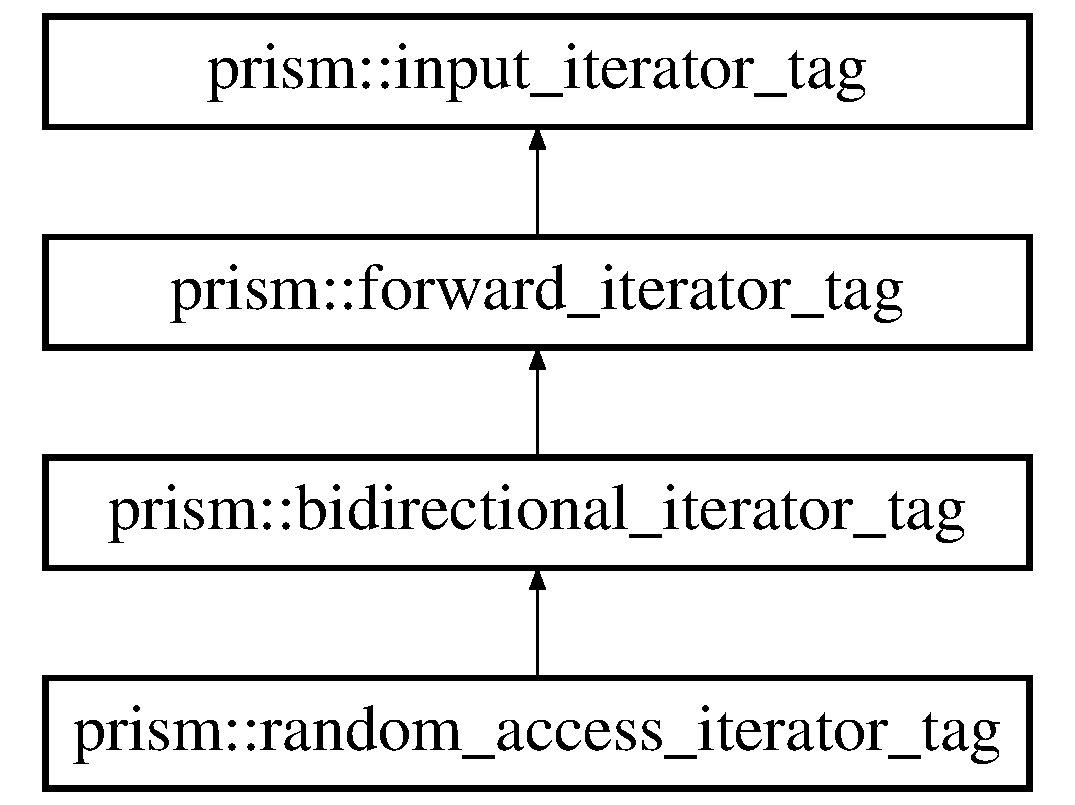
\includegraphics[height=4.000000cm]{structprism_1_1random__access__iterator__tag}
\end{center}
\end{figure}


The documentation for this struct was generated from the following file\+:\begin{DoxyCompactItemize}
\item 
inc/prism/h/\hyperlink{_iterator_8h}{Iterator.\+h}\end{DoxyCompactItemize}

\hypertarget{structprism_1_1_allocator_1_1rebind}{}\section{prism\+:\+:Allocator$<$ T $>$\+:\+:rebind$<$ U $>$ Struct Template Reference}
\label{structprism_1_1_allocator_1_1rebind}\index{prism\+::\+Allocator$<$ T $>$\+::rebind$<$ U $>$@{prism\+::\+Allocator$<$ T $>$\+::rebind$<$ U $>$}}
\subsection*{Public Types}
\begin{DoxyCompactItemize}
\item 
typedef \hyperlink{classprism_1_1_allocator}{Allocator}$<$ U $>$ \hyperlink{structprism_1_1_allocator_1_1rebind_a67ad1b0f9c61151a3063a742b411ccc3}{other}
\end{DoxyCompactItemize}


\subsection{Member Typedef Documentation}
\index{prism\+::\+Allocator\+::rebind@{prism\+::\+Allocator\+::rebind}!other@{other}}
\index{other@{other}!prism\+::\+Allocator\+::rebind@{prism\+::\+Allocator\+::rebind}}
\subsubsection[{\texorpdfstring{other}{other}}]{\setlength{\rightskip}{0pt plus 5cm}template$<$class T$>$ template$<$class U $>$ typedef {\bf Allocator}$<$U$>$ {\bf prism\+::\+Allocator}$<$ T $>$\+::{\bf rebind}$<$ U $>$\+::{\bf other}}\hypertarget{structprism_1_1_allocator_1_1rebind_a67ad1b0f9c61151a3063a742b411ccc3}{}\label{structprism_1_1_allocator_1_1rebind_a67ad1b0f9c61151a3063a742b411ccc3}


The documentation for this struct was generated from the following file\+:\begin{DoxyCompactItemize}
\item 
\hyperlink{_allocator_8h}{Allocator.\+h}\end{DoxyCompactItemize}

\hypertarget{structprism_1_1_log_allocator_1_1rebind}{}\section{prism\+:\+:Log\+Allocator$<$ T $>$\+:\+:rebind$<$ U $>$ Struct Template Reference}
\label{structprism_1_1_log_allocator_1_1rebind}\index{prism\+::\+Log\+Allocator$<$ T $>$\+::rebind$<$ U $>$@{prism\+::\+Log\+Allocator$<$ T $>$\+::rebind$<$ U $>$}}
\subsection*{Public Types}
\begin{DoxyCompactItemize}
\item 
typedef \hyperlink{classprism_1_1_log_allocator}{Log\+Allocator}$<$ U $>$ \hyperlink{structprism_1_1_log_allocator_1_1rebind_a72f405cf30fe3b5bd36da818f4e532c8}{other}
\end{DoxyCompactItemize}


\subsection{Member Typedef Documentation}
\index{prism\+::\+Log\+Allocator\+::rebind@{prism\+::\+Log\+Allocator\+::rebind}!other@{other}}
\index{other@{other}!prism\+::\+Log\+Allocator\+::rebind@{prism\+::\+Log\+Allocator\+::rebind}}
\subsubsection[{\texorpdfstring{other}{other}}]{\setlength{\rightskip}{0pt plus 5cm}template$<$class T$>$ template$<$class U $>$ typedef {\bf Log\+Allocator}$<$U$>$ {\bf prism\+::\+Log\+Allocator}$<$ T $>$\+::{\bf rebind}$<$ U $>$\+::{\bf other}}\hypertarget{structprism_1_1_log_allocator_1_1rebind_a72f405cf30fe3b5bd36da818f4e532c8}{}\label{structprism_1_1_log_allocator_1_1rebind_a72f405cf30fe3b5bd36da818f4e532c8}


The documentation for this struct was generated from the following file\+:\begin{DoxyCompactItemize}
\item 
\hyperlink{_log_allocator_8h}{Log\+Allocator.\+h}\end{DoxyCompactItemize}

\hypertarget{classprism_1_1_rect}{}\section{prism\+:\+:Rect Class Reference}
\label{classprism_1_1_rect}\index{prism\+::\+Rect@{prism\+::\+Rect}}


{\ttfamily \#include $<$Rect.\+h$>$}

\subsection*{Public Member Functions}
\begin{DoxyCompactItemize}
\item 
\hyperlink{classprism_1_1_rect_af61646ec28b099ffe1b4901ae5639662}{Rect} ()
\item 
\hyperlink{classprism_1_1_rect_a80055d4dfd1f9feb803a4419cd43671d}{Rect} (const int \hyperlink{classprism_1_1_rect_a202fa9a56964c9111a968fb9b420f5f4}{x}, const int \hyperlink{classprism_1_1_rect_a6e951744e0bba0fed781b86ab0be680b}{y}, const int \hyperlink{classprism_1_1_rect_a8dae47a50fdac7a5f7e8aabef68437aa}{width}, const int \hyperlink{classprism_1_1_rect_ad713f4536accdc6d5d2e6a6d83eac78b}{height})
\item 
\hyperlink{classprism_1_1_rect_a62e6eaa2eba9506e830bd6f3ff817bca}{Rect} (const \hyperlink{classprism_1_1_point}{Point} \&\hyperlink{classprism_1_1_rect_a2900a6e837124886d2e6aa500fba5bde}{top\+Left}, const \hyperlink{classprism_1_1_point}{Point} \&\hyperlink{classprism_1_1_rect_a97eb5a66441a49c7e149229376aba6a0}{bottom\+Right})
\item 
\hyperlink{classprism_1_1_rect_afda4a2a6cc3bdfd2e4e213813f6d0653}{Rect} (const \hyperlink{classprism_1_1_point}{Point} \&\hyperlink{classprism_1_1_rect_a2900a6e837124886d2e6aa500fba5bde}{top\+Left}, const \hyperlink{classprism_1_1_size}{Size} \&\hyperlink{classprism_1_1_rect_adcbe6d279ad57294c88d287057867a2b}{size})
\item 
\hyperlink{classprism_1_1_rect_a03f9f2832b8f325ded900d85b2d12ea3}{Rect} (const \hyperlink{classprism_1_1_rect}{Rect} \&\hyperlink{namespaceprism_ae776f4cd825f79e7af1cf6ee1d90a209}{copy})
\item 
virtual \hyperlink{classprism_1_1_rect_acf86bebcd76de609a3619b063de6a7fe}{$\sim$\+Rect} ()
\item 
void \hyperlink{classprism_1_1_rect_a8bbcfbe99d39f7350dc7801ed5cf6d48}{adjust} (const int dx1, const int dy1, const int dx2, const int dy2)
\item 
\hyperlink{classprism_1_1_rect}{Rect} \hyperlink{classprism_1_1_rect_aa0101c79f105eb2b988d3814e00be511}{adjusted} (const int dx1, const int dy1, const int dx2, const int dy2) const 
\item 
const int \hyperlink{classprism_1_1_rect_a8a6f1fbe20a10549a5ab9b85e04f209c}{bottom} () const 
\item 
\hyperlink{classprism_1_1_point}{Point} \hyperlink{classprism_1_1_rect_a561c86db589efaafbca149cdc11c5759}{bottom\+Left} () const 
\item 
\hyperlink{classprism_1_1_point}{Point} \hyperlink{classprism_1_1_rect_a97eb5a66441a49c7e149229376aba6a0}{bottom\+Right} () const 
\item 
\hyperlink{classprism_1_1_point}{Point} \hyperlink{classprism_1_1_rect_aacf848f3301590ab85fd803d72301af7}{centre} () const 
\item 
const bool \hyperlink{classprism_1_1_rect_a85cd85c5299edb5cc07cda4cf7733256}{contains} (const \hyperlink{classprism_1_1_point}{Point} \&point) const 
\item 
const bool \hyperlink{classprism_1_1_rect_ab92f880c4cb90b1aa382d8217d19d391}{contains} (const int \hyperlink{classprism_1_1_rect_a202fa9a56964c9111a968fb9b420f5f4}{x}, const int \hyperlink{classprism_1_1_rect_a6e951744e0bba0fed781b86ab0be680b}{y}) const 
\item 
const bool \hyperlink{classprism_1_1_rect_a64af57e3a62339a8b1760b51d5a76809}{contains} (const \hyperlink{classprism_1_1_rect}{Rect} \&rect) const 
\item 
void \hyperlink{classprism_1_1_rect_a20e7825273f653914b1e3bc9954e7deb}{get\+Coordinates} (int $\ast$x1, int $\ast$y1, int $\ast$x2, int $\ast$y2) const 
\item 
void \hyperlink{classprism_1_1_rect_a24f54f589f54d555c623c3db8a169047}{get\+Rect} (int $\ast$\hyperlink{classprism_1_1_rect_a202fa9a56964c9111a968fb9b420f5f4}{x}, int $\ast$\hyperlink{classprism_1_1_rect_a6e951744e0bba0fed781b86ab0be680b}{y}, int $\ast$\hyperlink{classprism_1_1_rect_a8dae47a50fdac7a5f7e8aabef68437aa}{width}, int $\ast$\hyperlink{classprism_1_1_rect_ad713f4536accdc6d5d2e6a6d83eac78b}{height}) const 
\item 
const int \hyperlink{classprism_1_1_rect_ad713f4536accdc6d5d2e6a6d83eac78b}{height} () const 
\item 
\hyperlink{classprism_1_1_rect}{Rect} \hyperlink{classprism_1_1_rect_a25ab32467c418ae6ee84df7ae759851a}{intersected} (const \hyperlink{classprism_1_1_rect}{Rect} \&rect) const 
\item 
const bool \hyperlink{classprism_1_1_rect_a291145fd95310946e84a009646d1540a}{intersects} (const \hyperlink{classprism_1_1_rect}{Rect} \&rect) const 
\item 
const bool \hyperlink{classprism_1_1_rect_aeaebf58b96d705192d3550fb085b5338}{is\+Empty} () const 
\item 
const bool \hyperlink{classprism_1_1_rect_a5bcde85987680d025c52f028fb8cbcea}{is\+Null} () const 
\item 
const bool \hyperlink{classprism_1_1_rect_a7a864d1c2f55c2758d05e23f131a2364}{is\+Valid} () const 
\item 
const int \hyperlink{classprism_1_1_rect_a75ddb96d128ac7b913865be7dbcd865e}{left} () const 
\item 
void \hyperlink{classprism_1_1_rect_ad9305fe8528c64db65ef9bd34c3578b8}{move\+Bottom} (const int \hyperlink{classprism_1_1_rect_a6e951744e0bba0fed781b86ab0be680b}{y})
\item 
void \hyperlink{classprism_1_1_rect_adbbb1cabc46780b605f3400c5ee4e39e}{move\+Bottom\+Left} (const \hyperlink{classprism_1_1_point}{Point} \&position)
\item 
void \hyperlink{classprism_1_1_rect_a88696414c9cbcc840805482d09a83e65}{move\+Bottom\+Right} (const \hyperlink{classprism_1_1_point}{Point} \&position)
\item 
void \hyperlink{classprism_1_1_rect_a4de806d7ddbe4ec946aef7843e5b4ac7}{move\+Centre} (const int \hyperlink{classprism_1_1_rect_a202fa9a56964c9111a968fb9b420f5f4}{x}, const int \hyperlink{classprism_1_1_rect_a6e951744e0bba0fed781b86ab0be680b}{y})
\item 
void \hyperlink{classprism_1_1_rect_a14862b09cf80442e9a4a9996ace251d0}{move\+Centre} (const \hyperlink{classprism_1_1_point}{Point} \&position)
\item 
void \hyperlink{classprism_1_1_rect_af1d84466fd81536d7fcd1a9e3084a8cb}{move\+Left} (const int \hyperlink{classprism_1_1_rect_a202fa9a56964c9111a968fb9b420f5f4}{x})
\item 
void \hyperlink{classprism_1_1_rect_a3da54bd285c3c4aae449b276cca81c29}{move\+Right} (const int \hyperlink{classprism_1_1_rect_a202fa9a56964c9111a968fb9b420f5f4}{x})
\item 
void \hyperlink{classprism_1_1_rect_aa89a93ae63e2fd0dae063509f588f253}{move\+To} (const int \hyperlink{classprism_1_1_rect_a202fa9a56964c9111a968fb9b420f5f4}{x}, const int \hyperlink{classprism_1_1_rect_a6e951744e0bba0fed781b86ab0be680b}{y})
\item 
void \hyperlink{classprism_1_1_rect_a7ee7a73b5cba4d3e3fcd048d77bceaa8}{move\+To} (const \hyperlink{classprism_1_1_point}{Point} \&position)
\item 
void \hyperlink{classprism_1_1_rect_a1b1e4d524a29d32eab8c0938b6ae5246}{move\+Top} (const int \hyperlink{classprism_1_1_rect_a6e951744e0bba0fed781b86ab0be680b}{y})
\item 
void \hyperlink{classprism_1_1_rect_ae0ccad0d81dbda985be4e9ee8ae3f6f7}{move\+Top\+Left} (const \hyperlink{classprism_1_1_point}{Point} \&position)
\item 
void \hyperlink{classprism_1_1_rect_a24bdcf4de55d61b8c41010a8614203a7}{move\+Top\+Right} (const \hyperlink{classprism_1_1_point}{Point} \&position)
\item 
\hyperlink{classprism_1_1_rect}{Rect} \hyperlink{classprism_1_1_rect_ab08d9dbc02f86349530e0a2b6f6d05d6}{normalised} () const 
\item 
const int \hyperlink{classprism_1_1_rect_abf19c427e016b65d28118b8330de62d1}{right} () const 
\item 
void \hyperlink{classprism_1_1_rect_ac9d82a69be0dba946f8f9421aa33fffe}{set\+Bottom} (const int \hyperlink{classprism_1_1_rect_a6e951744e0bba0fed781b86ab0be680b}{y})
\item 
void \hyperlink{classprism_1_1_rect_a467b2b59e56d1aee949d9fb32681d559}{set\+Bottom\+Left} (const \hyperlink{classprism_1_1_point}{Point} \&position)
\item 
void \hyperlink{classprism_1_1_rect_a681ef54c0d6e0fac56394f15623c764f}{set\+Bottom\+Right} (const \hyperlink{classprism_1_1_point}{Point} \&position)
\item 
void \hyperlink{classprism_1_1_rect_ac930da7066defdd4646d801edc0b1cc0}{set\+Coordinates} (const int x1, const int y1, const int x2, const int y2)
\item 
void \hyperlink{classprism_1_1_rect_a0358cb30610f6bacde57613840bb5f4c}{set\+Height} (const int \hyperlink{classprism_1_1_rect_ad713f4536accdc6d5d2e6a6d83eac78b}{height})
\item 
void \hyperlink{classprism_1_1_rect_a58f42232724615d479b4cc3a08eeac01}{set\+Left} (const int \hyperlink{classprism_1_1_rect_a202fa9a56964c9111a968fb9b420f5f4}{x})
\item 
void \hyperlink{classprism_1_1_rect_a32978009107a8c2ea4787edde3960985}{set\+Rect} (const int \hyperlink{classprism_1_1_rect_a202fa9a56964c9111a968fb9b420f5f4}{x}, const int \hyperlink{classprism_1_1_rect_a6e951744e0bba0fed781b86ab0be680b}{y}, const int \hyperlink{classprism_1_1_rect_a8dae47a50fdac7a5f7e8aabef68437aa}{width}, const int \hyperlink{classprism_1_1_rect_ad713f4536accdc6d5d2e6a6d83eac78b}{height})
\item 
void \hyperlink{classprism_1_1_rect_a2e43d5a19fddd80fdbcee1c8892a775d}{set\+Right} (const int \hyperlink{classprism_1_1_rect_a202fa9a56964c9111a968fb9b420f5f4}{x})
\item 
void \hyperlink{classprism_1_1_rect_a53275ba29c1cdb4db5a728f26eae9662}{set\+Size} (const \hyperlink{classprism_1_1_size}{Size} \&\hyperlink{classprism_1_1_rect_adcbe6d279ad57294c88d287057867a2b}{size})
\item 
void \hyperlink{classprism_1_1_rect_afb4e4ead74ed1d0bf300fb37266b47d4}{set\+Top} (const int \hyperlink{classprism_1_1_rect_a6e951744e0bba0fed781b86ab0be680b}{y})
\item 
void \hyperlink{classprism_1_1_rect_ae417c702d2ae34b49bb98d38c4b769a4}{set\+Top\+Left} (const \hyperlink{classprism_1_1_point}{Point} \&position)
\item 
void \hyperlink{classprism_1_1_rect_a160eff655569c91544cb4559663b7397}{set\+Top\+Right} (const \hyperlink{classprism_1_1_point}{Point} \&position)
\item 
void \hyperlink{classprism_1_1_rect_a52362693dd88bececa0ee8083e316792}{setX} (const int \hyperlink{classprism_1_1_rect_a202fa9a56964c9111a968fb9b420f5f4}{x})
\item 
void \hyperlink{classprism_1_1_rect_a4a55e496695d8ccbcadd49305bf22617}{setY} (const int \hyperlink{classprism_1_1_rect_a6e951744e0bba0fed781b86ab0be680b}{y})
\item 
void \hyperlink{classprism_1_1_rect_a8e6c00c46158a9c993e7fb33f3d8befd}{set\+Width} (const int \hyperlink{classprism_1_1_rect_a8dae47a50fdac7a5f7e8aabef68437aa}{width})
\item 
\hyperlink{classprism_1_1_size}{Size} \hyperlink{classprism_1_1_rect_adcbe6d279ad57294c88d287057867a2b}{size} () const 
\item 
const int \hyperlink{classprism_1_1_rect_a1e89336f88213ac0672643d188133bab}{top} () const 
\item 
\hyperlink{classprism_1_1_point}{Point} \hyperlink{classprism_1_1_rect_a2900a6e837124886d2e6aa500fba5bde}{top\+Left} () const 
\item 
\hyperlink{classprism_1_1_point}{Point} \hyperlink{classprism_1_1_rect_a0a5e7ccdaeb397649e1e9331110a7343}{top\+Right} () const 
\item 
void \hyperlink{classprism_1_1_rect_a18f564924e2d800589ddf8af039fa248}{translate} (const int dx, const int dy)
\item 
void \hyperlink{classprism_1_1_rect_ab4fd05471a4321adf84dadefa85668b7}{translate} (const \hyperlink{classprism_1_1_point}{Point} \&offset)
\item 
\hyperlink{classprism_1_1_rect}{Rect} \hyperlink{classprism_1_1_rect_accc97050ae8799c21cd64500b1a783dd}{translated} (const int dx, const int dy) const 
\item 
\hyperlink{classprism_1_1_rect}{Rect} \hyperlink{classprism_1_1_rect_ac71993c5f890157af1e3fa86423f8198}{translated} (const \hyperlink{classprism_1_1_point}{Point} \&offset) const 
\item 
\hyperlink{classprism_1_1_rect}{Rect} \hyperlink{classprism_1_1_rect_aa4f9bf21ac8c5a1d1b415df78ef5c0da}{transposed} () const 
\item 
\hyperlink{classprism_1_1_rect}{Rect} \hyperlink{classprism_1_1_rect_ac938b0ebead7062111728b6d2392e38a}{united} (const \hyperlink{classprism_1_1_rect}{Rect} \&rect) const 
\item 
const int \hyperlink{classprism_1_1_rect_a8dae47a50fdac7a5f7e8aabef68437aa}{width} () const 
\item 
const int \hyperlink{classprism_1_1_rect_a202fa9a56964c9111a968fb9b420f5f4}{x} () const 
\item 
const int \hyperlink{classprism_1_1_rect_a6e951744e0bba0fed781b86ab0be680b}{y} () const 
\item 
\hyperlink{classprism_1_1_rect}{Rect} \& \hyperlink{classprism_1_1_rect_a1addf86103e655c776e4e20dd3c97a84}{operator=} (const \hyperlink{classprism_1_1_rect}{Rect} \&rect)
\end{DoxyCompactItemize}
\subsection*{Friends}
\begin{DoxyCompactItemize}
\item 
const bool \hyperlink{classprism_1_1_rect_ab32eafa53d6e2fedc5c4f4beeb10d12a}{operator==} (const \hyperlink{classprism_1_1_rect}{Rect} \&r1, const \hyperlink{classprism_1_1_rect}{Rect} \&r2)
\item 
const bool \hyperlink{classprism_1_1_rect_a649643043218228aae2b7d95e1a95dba}{operator!=} (const \hyperlink{classprism_1_1_rect}{Rect} \&r1, const \hyperlink{classprism_1_1_rect}{Rect} \&r2)
\item 
std\+::ostream \& \hyperlink{classprism_1_1_rect_a729ddc4e5633a601a2813d124209056f}{operator$<$$<$} (std\+::ostream \&out, const \hyperlink{classprism_1_1_rect}{Rect} \&rect)
\end{DoxyCompactItemize}


\subsection{Constructor \& Destructor Documentation}
\index{prism\+::\+Rect@{prism\+::\+Rect}!Rect@{Rect}}
\index{Rect@{Rect}!prism\+::\+Rect@{prism\+::\+Rect}}
\subsubsection[{\texorpdfstring{Rect()}{Rect()}}]{\setlength{\rightskip}{0pt plus 5cm}prism\+::\+Rect\+::\+Rect (
\begin{DoxyParamCaption}
{}
\end{DoxyParamCaption}
)}\hypertarget{classprism_1_1_rect_af61646ec28b099ffe1b4901ae5639662}{}\label{classprism_1_1_rect_af61646ec28b099ffe1b4901ae5639662}
Creates a rectangle with x=y=width=height=0. {\itshape \hyperlink{classprism_1_1_rect_aeaebf58b96d705192d3550fb085b5338}{is\+Empty()}} and {\itshape \hyperlink{classprism_1_1_rect_a5bcde85987680d025c52f028fb8cbcea}{is\+Null()}} will return true in this state whilst {\itshape \hyperlink{classprism_1_1_rect_a7a864d1c2f55c2758d05e23f131a2364}{is\+Valid()}} will return false. \index{prism\+::\+Rect@{prism\+::\+Rect}!Rect@{Rect}}
\index{Rect@{Rect}!prism\+::\+Rect@{prism\+::\+Rect}}
\subsubsection[{\texorpdfstring{Rect(const int x, const int y, const int width, const int height)}{Rect(const int x, const int y, const int width, const int height)}}]{\setlength{\rightskip}{0pt plus 5cm}prism\+::\+Rect\+::\+Rect (
\begin{DoxyParamCaption}
\item[{const int}]{x, }
\item[{const int}]{y, }
\item[{const int}]{width, }
\item[{const int}]{height}
\end{DoxyParamCaption}
)}\hypertarget{classprism_1_1_rect_a80055d4dfd1f9feb803a4419cd43671d}{}\label{classprism_1_1_rect_a80055d4dfd1f9feb803a4419cd43671d}
Creates a rectangle positioning the top left corner at (x,y) and having {\itshape width} and {\itshape height}. \index{prism\+::\+Rect@{prism\+::\+Rect}!Rect@{Rect}}
\index{Rect@{Rect}!prism\+::\+Rect@{prism\+::\+Rect}}
\subsubsection[{\texorpdfstring{Rect(const Point \&top\+Left, const Point \&bottom\+Right)}{Rect(const Point &topLeft, const Point &bottomRight)}}]{\setlength{\rightskip}{0pt plus 5cm}prism\+::\+Rect\+::\+Rect (
\begin{DoxyParamCaption}
\item[{const {\bf Point} \&}]{top\+Left, }
\item[{const {\bf Point} \&}]{bottom\+Right}
\end{DoxyParamCaption}
)}\hypertarget{classprism_1_1_rect_a62e6eaa2eba9506e830bd6f3ff817bca}{}\label{classprism_1_1_rect_a62e6eaa2eba9506e830bd6f3ff817bca}
Creates a rectangle positioning its top left corner at {\itshape top\+Left} and its bottom right corner positioned at {\itshape bottom\+Right}. \index{prism\+::\+Rect@{prism\+::\+Rect}!Rect@{Rect}}
\index{Rect@{Rect}!prism\+::\+Rect@{prism\+::\+Rect}}
\subsubsection[{\texorpdfstring{Rect(const Point \&top\+Left, const Size \&size)}{Rect(const Point &topLeft, const Size &size)}}]{\setlength{\rightskip}{0pt plus 5cm}prism\+::\+Rect\+::\+Rect (
\begin{DoxyParamCaption}
\item[{const {\bf Point} \&}]{top\+Left, }
\item[{const {\bf Size} \&}]{size}
\end{DoxyParamCaption}
)}\hypertarget{classprism_1_1_rect_afda4a2a6cc3bdfd2e4e213813f6d0653}{}\label{classprism_1_1_rect_afda4a2a6cc3bdfd2e4e213813f6d0653}
Creates a rectangle positioning its top left corner at {\itshape top\+Left} and its width and height set to {\itshape size}. \index{prism\+::\+Rect@{prism\+::\+Rect}!Rect@{Rect}}
\index{Rect@{Rect}!prism\+::\+Rect@{prism\+::\+Rect}}
\subsubsection[{\texorpdfstring{Rect(const Rect \&copy)}{Rect(const Rect &copy)}}]{\setlength{\rightskip}{0pt plus 5cm}prism\+::\+Rect\+::\+Rect (
\begin{DoxyParamCaption}
\item[{const {\bf Rect} \&}]{copy}
\end{DoxyParamCaption}
)}\hypertarget{classprism_1_1_rect_a03f9f2832b8f325ded900d85b2d12ea3}{}\label{classprism_1_1_rect_a03f9f2832b8f325ded900d85b2d12ea3}
Copy constructor makes a copy of {\itshape copy}. \index{prism\+::\+Rect@{prism\+::\+Rect}!````~Rect@{$\sim$\+Rect}}
\index{````~Rect@{$\sim$\+Rect}!prism\+::\+Rect@{prism\+::\+Rect}}
\subsubsection[{\texorpdfstring{$\sim$\+Rect()}{~Rect()}}]{\setlength{\rightskip}{0pt plus 5cm}prism\+::\+Rect\+::$\sim$\+Rect (
\begin{DoxyParamCaption}
{}
\end{DoxyParamCaption}
)\hspace{0.3cm}{\ttfamily [virtual]}}\hypertarget{classprism_1_1_rect_acf86bebcd76de609a3619b063de6a7fe}{}\label{classprism_1_1_rect_acf86bebcd76de609a3619b063de6a7fe}
Destroys the rectangle. 

\subsection{Member Function Documentation}
\index{prism\+::\+Rect@{prism\+::\+Rect}!adjust@{adjust}}
\index{adjust@{adjust}!prism\+::\+Rect@{prism\+::\+Rect}}
\subsubsection[{\texorpdfstring{adjust(const int dx1, const int dy1, const int dx2, const int dy2)}{adjust(const int dx1, const int dy1, const int dx2, const int dy2)}}]{\setlength{\rightskip}{0pt plus 5cm}void prism\+::\+Rect\+::adjust (
\begin{DoxyParamCaption}
\item[{const int}]{dx1, }
\item[{const int}]{dy1, }
\item[{const int}]{dx2, }
\item[{const int}]{dy2}
\end{DoxyParamCaption}
)}\hypertarget{classprism_1_1_rect_a8bbcfbe99d39f7350dc7801ed5cf6d48}{}\label{classprism_1_1_rect_a8bbcfbe99d39f7350dc7801ed5cf6d48}
Adds dx1, dy1, dx2 and dy2 to the existing coordinates of the rectangle. \index{prism\+::\+Rect@{prism\+::\+Rect}!adjusted@{adjusted}}
\index{adjusted@{adjusted}!prism\+::\+Rect@{prism\+::\+Rect}}
\subsubsection[{\texorpdfstring{adjusted(const int dx1, const int dy1, const int dx2, const int dy2) const }{adjusted(const int dx1, const int dy1, const int dx2, const int dy2) const }}]{\setlength{\rightskip}{0pt plus 5cm}{\bf Rect} prism\+::\+Rect\+::adjusted (
\begin{DoxyParamCaption}
\item[{const int}]{dx1, }
\item[{const int}]{dy1, }
\item[{const int}]{dx2, }
\item[{const int}]{dy2}
\end{DoxyParamCaption}
) const}\hypertarget{classprism_1_1_rect_aa0101c79f105eb2b988d3814e00be511}{}\label{classprism_1_1_rect_aa0101c79f105eb2b988d3814e00be511}
Returns a copy of this rectangle which has added dx1, dy1, dx2 and dy2 to the existing coordinates of the rectangle. \index{prism\+::\+Rect@{prism\+::\+Rect}!bottom@{bottom}}
\index{bottom@{bottom}!prism\+::\+Rect@{prism\+::\+Rect}}
\subsubsection[{\texorpdfstring{bottom() const }{bottom() const }}]{\setlength{\rightskip}{0pt plus 5cm}const int prism\+::\+Rect\+::bottom (
\begin{DoxyParamCaption}
{}
\end{DoxyParamCaption}
) const}\hypertarget{classprism_1_1_rect_a8a6f1fbe20a10549a5ab9b85e04f209c}{}\label{classprism_1_1_rect_a8a6f1fbe20a10549a5ab9b85e04f209c}
Returns the y-\/coordinate of the rectangle\textquotesingle{}s bottom edge. \index{prism\+::\+Rect@{prism\+::\+Rect}!bottom\+Left@{bottom\+Left}}
\index{bottom\+Left@{bottom\+Left}!prism\+::\+Rect@{prism\+::\+Rect}}
\subsubsection[{\texorpdfstring{bottom\+Left() const }{bottomLeft() const }}]{\setlength{\rightskip}{0pt plus 5cm}{\bf Point} prism\+::\+Rect\+::bottom\+Left (
\begin{DoxyParamCaption}
{}
\end{DoxyParamCaption}
) const}\hypertarget{classprism_1_1_rect_a561c86db589efaafbca149cdc11c5759}{}\label{classprism_1_1_rect_a561c86db589efaafbca149cdc11c5759}
Returns the coordinate of the bottom left of the rectangle. \index{prism\+::\+Rect@{prism\+::\+Rect}!bottom\+Right@{bottom\+Right}}
\index{bottom\+Right@{bottom\+Right}!prism\+::\+Rect@{prism\+::\+Rect}}
\subsubsection[{\texorpdfstring{bottom\+Right() const }{bottomRight() const }}]{\setlength{\rightskip}{0pt plus 5cm}{\bf Point} prism\+::\+Rect\+::bottom\+Right (
\begin{DoxyParamCaption}
{}
\end{DoxyParamCaption}
) const}\hypertarget{classprism_1_1_rect_a97eb5a66441a49c7e149229376aba6a0}{}\label{classprism_1_1_rect_a97eb5a66441a49c7e149229376aba6a0}
Returns the coordinate of the bottom right of the rectangle. \index{prism\+::\+Rect@{prism\+::\+Rect}!centre@{centre}}
\index{centre@{centre}!prism\+::\+Rect@{prism\+::\+Rect}}
\subsubsection[{\texorpdfstring{centre() const }{centre() const }}]{\setlength{\rightskip}{0pt plus 5cm}{\bf Point} prism\+::\+Rect\+::centre (
\begin{DoxyParamCaption}
{}
\end{DoxyParamCaption}
) const}\hypertarget{classprism_1_1_rect_aacf848f3301590ab85fd803d72301af7}{}\label{classprism_1_1_rect_aacf848f3301590ab85fd803d72301af7}
Returns the coordinate of the centre point of the rectangle. \index{prism\+::\+Rect@{prism\+::\+Rect}!contains@{contains}}
\index{contains@{contains}!prism\+::\+Rect@{prism\+::\+Rect}}
\subsubsection[{\texorpdfstring{contains(const Point \&point) const }{contains(const Point &point) const }}]{\setlength{\rightskip}{0pt plus 5cm}const bool prism\+::\+Rect\+::contains (
\begin{DoxyParamCaption}
\item[{const {\bf Point} \&}]{point}
\end{DoxyParamCaption}
) const}\hypertarget{classprism_1_1_rect_a85cd85c5299edb5cc07cda4cf7733256}{}\label{classprism_1_1_rect_a85cd85c5299edb5cc07cda4cf7733256}
Returns true if {\itshape point} is within or on the rectangle\textquotesingle{}s boundary, false otherwise. \index{prism\+::\+Rect@{prism\+::\+Rect}!contains@{contains}}
\index{contains@{contains}!prism\+::\+Rect@{prism\+::\+Rect}}
\subsubsection[{\texorpdfstring{contains(const int x, const int y) const }{contains(const int x, const int y) const }}]{\setlength{\rightskip}{0pt plus 5cm}const bool prism\+::\+Rect\+::contains (
\begin{DoxyParamCaption}
\item[{const int}]{x, }
\item[{const int}]{y}
\end{DoxyParamCaption}
) const}\hypertarget{classprism_1_1_rect_ab92f880c4cb90b1aa382d8217d19d391}{}\label{classprism_1_1_rect_ab92f880c4cb90b1aa382d8217d19d391}
Returns true if (x,y) is within or on the rectangle\textquotesingle{}s boundary, false otherwise. \index{prism\+::\+Rect@{prism\+::\+Rect}!contains@{contains}}
\index{contains@{contains}!prism\+::\+Rect@{prism\+::\+Rect}}
\subsubsection[{\texorpdfstring{contains(const Rect \&rect) const }{contains(const Rect &rect) const }}]{\setlength{\rightskip}{0pt plus 5cm}const bool prism\+::\+Rect\+::contains (
\begin{DoxyParamCaption}
\item[{const {\bf Rect} \&}]{rect}
\end{DoxyParamCaption}
) const}\hypertarget{classprism_1_1_rect_a64af57e3a62339a8b1760b51d5a76809}{}\label{classprism_1_1_rect_a64af57e3a62339a8b1760b51d5a76809}
Returns true if {\itshape rect} is contained within or on the rectangle\textquotesingle{}s boundary, false otherwise. \index{prism\+::\+Rect@{prism\+::\+Rect}!get\+Coordinates@{get\+Coordinates}}
\index{get\+Coordinates@{get\+Coordinates}!prism\+::\+Rect@{prism\+::\+Rect}}
\subsubsection[{\texorpdfstring{get\+Coordinates(int $\ast$x1, int $\ast$y1, int $\ast$x2, int $\ast$y2) const }{getCoordinates(int *x1, int *y1, int *x2, int *y2) const }}]{\setlength{\rightskip}{0pt plus 5cm}void prism\+::\+Rect\+::get\+Coordinates (
\begin{DoxyParamCaption}
\item[{int $\ast$}]{x1, }
\item[{int $\ast$}]{y1, }
\item[{int $\ast$}]{x2, }
\item[{int $\ast$}]{y2}
\end{DoxyParamCaption}
) const}\hypertarget{classprism_1_1_rect_a20e7825273f653914b1e3bc9954e7deb}{}\label{classprism_1_1_rect_a20e7825273f653914b1e3bc9954e7deb}
Extracts the coordinates of the rectangle and assigns them to (x1,y1)(x2,y2). \index{prism\+::\+Rect@{prism\+::\+Rect}!get\+Rect@{get\+Rect}}
\index{get\+Rect@{get\+Rect}!prism\+::\+Rect@{prism\+::\+Rect}}
\subsubsection[{\texorpdfstring{get\+Rect(int $\ast$x, int $\ast$y, int $\ast$width, int $\ast$height) const }{getRect(int *x, int *y, int *width, int *height) const }}]{\setlength{\rightskip}{0pt plus 5cm}void prism\+::\+Rect\+::get\+Rect (
\begin{DoxyParamCaption}
\item[{int $\ast$}]{x, }
\item[{int $\ast$}]{y, }
\item[{int $\ast$}]{width, }
\item[{int $\ast$}]{height}
\end{DoxyParamCaption}
) const}\hypertarget{classprism_1_1_rect_a24f54f589f54d555c623c3db8a169047}{}\label{classprism_1_1_rect_a24f54f589f54d555c623c3db8a169047}
Extracts the top left corner coordinates and width and height of this rectangle and assigns them to (x,y) and {\itshape width} and {\itshape height}. \index{prism\+::\+Rect@{prism\+::\+Rect}!height@{height}}
\index{height@{height}!prism\+::\+Rect@{prism\+::\+Rect}}
\subsubsection[{\texorpdfstring{height() const }{height() const }}]{\setlength{\rightskip}{0pt plus 5cm}const int prism\+::\+Rect\+::height (
\begin{DoxyParamCaption}
{}
\end{DoxyParamCaption}
) const}\hypertarget{classprism_1_1_rect_ad713f4536accdc6d5d2e6a6d83eac78b}{}\label{classprism_1_1_rect_ad713f4536accdc6d5d2e6a6d83eac78b}
Returns the height of the rectangle. \index{prism\+::\+Rect@{prism\+::\+Rect}!intersected@{intersected}}
\index{intersected@{intersected}!prism\+::\+Rect@{prism\+::\+Rect}}
\subsubsection[{\texorpdfstring{intersected(const Rect \&rect) const }{intersected(const Rect &rect) const }}]{\setlength{\rightskip}{0pt plus 5cm}{\bf Rect} prism\+::\+Rect\+::intersected (
\begin{DoxyParamCaption}
\item[{const {\bf Rect} \&}]{rect}
\end{DoxyParamCaption}
) const}\hypertarget{classprism_1_1_rect_a25ab32467c418ae6ee84df7ae759851a}{}\label{classprism_1_1_rect_a25ab32467c418ae6ee84df7ae759851a}
Returns a rectangle that represents the overlapping portion of this rectangle and {\itshape rect}. If the two rectangles are not intersected then this rectangle is returned instead. \index{prism\+::\+Rect@{prism\+::\+Rect}!intersects@{intersects}}
\index{intersects@{intersects}!prism\+::\+Rect@{prism\+::\+Rect}}
\subsubsection[{\texorpdfstring{intersects(const Rect \&rect) const }{intersects(const Rect &rect) const }}]{\setlength{\rightskip}{0pt plus 5cm}const bool prism\+::\+Rect\+::intersects (
\begin{DoxyParamCaption}
\item[{const {\bf Rect} \&}]{rect}
\end{DoxyParamCaption}
) const}\hypertarget{classprism_1_1_rect_a291145fd95310946e84a009646d1540a}{}\label{classprism_1_1_rect_a291145fd95310946e84a009646d1540a}
Returns true if {\itshape rect} intersects this rectangle, false otherwise. Note that a rectangle must intersect by at least 1 pixel in order for it to be considered intersecting. Edges that sit on top of each are not considered to be intersecting. \index{prism\+::\+Rect@{prism\+::\+Rect}!is\+Empty@{is\+Empty}}
\index{is\+Empty@{is\+Empty}!prism\+::\+Rect@{prism\+::\+Rect}}
\subsubsection[{\texorpdfstring{is\+Empty() const }{isEmpty() const }}]{\setlength{\rightskip}{0pt plus 5cm}const bool prism\+::\+Rect\+::is\+Empty (
\begin{DoxyParamCaption}
{}
\end{DoxyParamCaption}
) const}\hypertarget{classprism_1_1_rect_aeaebf58b96d705192d3550fb085b5338}{}\label{classprism_1_1_rect_aeaebf58b96d705192d3550fb085b5338}
An empty rectangle is one where its width or height (or both) are zero or less. Returns true if it is an empy rectangle, false otherwise. \index{prism\+::\+Rect@{prism\+::\+Rect}!is\+Null@{is\+Null}}
\index{is\+Null@{is\+Null}!prism\+::\+Rect@{prism\+::\+Rect}}
\subsubsection[{\texorpdfstring{is\+Null() const }{isNull() const }}]{\setlength{\rightskip}{0pt plus 5cm}const bool prism\+::\+Rect\+::is\+Null (
\begin{DoxyParamCaption}
{}
\end{DoxyParamCaption}
) const}\hypertarget{classprism_1_1_rect_a5bcde85987680d025c52f028fb8cbcea}{}\label{classprism_1_1_rect_a5bcde85987680d025c52f028fb8cbcea}
A null rectangle is one where the width and height are both equal to zero. Returns true if it is a null rectangle, false otherwise. \index{prism\+::\+Rect@{prism\+::\+Rect}!is\+Valid@{is\+Valid}}
\index{is\+Valid@{is\+Valid}!prism\+::\+Rect@{prism\+::\+Rect}}
\subsubsection[{\texorpdfstring{is\+Valid() const }{isValid() const }}]{\setlength{\rightskip}{0pt plus 5cm}const bool prism\+::\+Rect\+::is\+Valid (
\begin{DoxyParamCaption}
{}
\end{DoxyParamCaption}
) const}\hypertarget{classprism_1_1_rect_a7a864d1c2f55c2758d05e23f131a2364}{}\label{classprism_1_1_rect_a7a864d1c2f55c2758d05e23f131a2364}
A valid rectangle is one where its width and height are at least 1 or greater. Returns true if this is a valid rectangle, false otherwise. \index{prism\+::\+Rect@{prism\+::\+Rect}!left@{left}}
\index{left@{left}!prism\+::\+Rect@{prism\+::\+Rect}}
\subsubsection[{\texorpdfstring{left() const }{left() const }}]{\setlength{\rightskip}{0pt plus 5cm}const int prism\+::\+Rect\+::left (
\begin{DoxyParamCaption}
{}
\end{DoxyParamCaption}
) const}\hypertarget{classprism_1_1_rect_a75ddb96d128ac7b913865be7dbcd865e}{}\label{classprism_1_1_rect_a75ddb96d128ac7b913865be7dbcd865e}
Returns the x-\/coordinate of the rectangle\textquotesingle{}s left edge. \index{prism\+::\+Rect@{prism\+::\+Rect}!move\+Bottom@{move\+Bottom}}
\index{move\+Bottom@{move\+Bottom}!prism\+::\+Rect@{prism\+::\+Rect}}
\subsubsection[{\texorpdfstring{move\+Bottom(const int y)}{moveBottom(const int y)}}]{\setlength{\rightskip}{0pt plus 5cm}void prism\+::\+Rect\+::move\+Bottom (
\begin{DoxyParamCaption}
\item[{const int}]{y}
\end{DoxyParamCaption}
)}\hypertarget{classprism_1_1_rect_ad9305fe8528c64db65ef9bd34c3578b8}{}\label{classprism_1_1_rect_ad9305fe8528c64db65ef9bd34c3578b8}
Moves the rectangle downwards so that its bottom edge is positioned at {\itshape y}. This does not affect the width and height. \index{prism\+::\+Rect@{prism\+::\+Rect}!move\+Bottom\+Left@{move\+Bottom\+Left}}
\index{move\+Bottom\+Left@{move\+Bottom\+Left}!prism\+::\+Rect@{prism\+::\+Rect}}
\subsubsection[{\texorpdfstring{move\+Bottom\+Left(const Point \&position)}{moveBottomLeft(const Point &position)}}]{\setlength{\rightskip}{0pt plus 5cm}void prism\+::\+Rect\+::move\+Bottom\+Left (
\begin{DoxyParamCaption}
\item[{const {\bf Point} \&}]{position}
\end{DoxyParamCaption}
)}\hypertarget{classprism_1_1_rect_adbbb1cabc46780b605f3400c5ee4e39e}{}\label{classprism_1_1_rect_adbbb1cabc46780b605f3400c5ee4e39e}
\index{prism\+::\+Rect@{prism\+::\+Rect}!move\+Bottom\+Right@{move\+Bottom\+Right}}
\index{move\+Bottom\+Right@{move\+Bottom\+Right}!prism\+::\+Rect@{prism\+::\+Rect}}
\subsubsection[{\texorpdfstring{move\+Bottom\+Right(const Point \&position)}{moveBottomRight(const Point &position)}}]{\setlength{\rightskip}{0pt plus 5cm}void prism\+::\+Rect\+::move\+Bottom\+Right (
\begin{DoxyParamCaption}
\item[{const {\bf Point} \&}]{position}
\end{DoxyParamCaption}
)}\hypertarget{classprism_1_1_rect_a88696414c9cbcc840805482d09a83e65}{}\label{classprism_1_1_rect_a88696414c9cbcc840805482d09a83e65}
\index{prism\+::\+Rect@{prism\+::\+Rect}!move\+Centre@{move\+Centre}}
\index{move\+Centre@{move\+Centre}!prism\+::\+Rect@{prism\+::\+Rect}}
\subsubsection[{\texorpdfstring{move\+Centre(const int x, const int y)}{moveCentre(const int x, const int y)}}]{\setlength{\rightskip}{0pt plus 5cm}void prism\+::\+Rect\+::move\+Centre (
\begin{DoxyParamCaption}
\item[{const int}]{x, }
\item[{const int}]{y}
\end{DoxyParamCaption}
)}\hypertarget{classprism_1_1_rect_a4de806d7ddbe4ec946aef7843e5b4ac7}{}\label{classprism_1_1_rect_a4de806d7ddbe4ec946aef7843e5b4ac7}
Moves the rectangle placing its centre at (x,y). This does not affect the width and height. \index{prism\+::\+Rect@{prism\+::\+Rect}!move\+Centre@{move\+Centre}}
\index{move\+Centre@{move\+Centre}!prism\+::\+Rect@{prism\+::\+Rect}}
\subsubsection[{\texorpdfstring{move\+Centre(const Point \&position)}{moveCentre(const Point &position)}}]{\setlength{\rightskip}{0pt plus 5cm}void prism\+::\+Rect\+::move\+Centre (
\begin{DoxyParamCaption}
\item[{const {\bf Point} \&}]{position}
\end{DoxyParamCaption}
)}\hypertarget{classprism_1_1_rect_a14862b09cf80442e9a4a9996ace251d0}{}\label{classprism_1_1_rect_a14862b09cf80442e9a4a9996ace251d0}
Moves the rectangle placing its centre point at {\itshape position}. This does not affect the width and height. \index{prism\+::\+Rect@{prism\+::\+Rect}!move\+Left@{move\+Left}}
\index{move\+Left@{move\+Left}!prism\+::\+Rect@{prism\+::\+Rect}}
\subsubsection[{\texorpdfstring{move\+Left(const int x)}{moveLeft(const int x)}}]{\setlength{\rightskip}{0pt plus 5cm}void prism\+::\+Rect\+::move\+Left (
\begin{DoxyParamCaption}
\item[{const int}]{x}
\end{DoxyParamCaption}
)}\hypertarget{classprism_1_1_rect_af1d84466fd81536d7fcd1a9e3084a8cb}{}\label{classprism_1_1_rect_af1d84466fd81536d7fcd1a9e3084a8cb}
Moves the rectangle to the left so that its left edge is positioned at {\itshape x}. This does not affect the width and height. \index{prism\+::\+Rect@{prism\+::\+Rect}!move\+Right@{move\+Right}}
\index{move\+Right@{move\+Right}!prism\+::\+Rect@{prism\+::\+Rect}}
\subsubsection[{\texorpdfstring{move\+Right(const int x)}{moveRight(const int x)}}]{\setlength{\rightskip}{0pt plus 5cm}void prism\+::\+Rect\+::move\+Right (
\begin{DoxyParamCaption}
\item[{const int}]{x}
\end{DoxyParamCaption}
)}\hypertarget{classprism_1_1_rect_a3da54bd285c3c4aae449b276cca81c29}{}\label{classprism_1_1_rect_a3da54bd285c3c4aae449b276cca81c29}
Moves the rectangle to the right so that its right edge is positioned at {\itshape x}. This does not affect the width and height. \index{prism\+::\+Rect@{prism\+::\+Rect}!move\+To@{move\+To}}
\index{move\+To@{move\+To}!prism\+::\+Rect@{prism\+::\+Rect}}
\subsubsection[{\texorpdfstring{move\+To(const int x, const int y)}{moveTo(const int x, const int y)}}]{\setlength{\rightskip}{0pt plus 5cm}void prism\+::\+Rect\+::move\+To (
\begin{DoxyParamCaption}
\item[{const int}]{x, }
\item[{const int}]{y}
\end{DoxyParamCaption}
)}\hypertarget{classprism_1_1_rect_aa89a93ae63e2fd0dae063509f588f253}{}\label{classprism_1_1_rect_aa89a93ae63e2fd0dae063509f588f253}
Moves the rectangle so that its top left corner will be located at (x,y). The width and height will still be the same as before the rectangle was moved. \index{prism\+::\+Rect@{prism\+::\+Rect}!move\+To@{move\+To}}
\index{move\+To@{move\+To}!prism\+::\+Rect@{prism\+::\+Rect}}
\subsubsection[{\texorpdfstring{move\+To(const Point \&position)}{moveTo(const Point &position)}}]{\setlength{\rightskip}{0pt plus 5cm}void prism\+::\+Rect\+::move\+To (
\begin{DoxyParamCaption}
\item[{const {\bf Point} \&}]{position}
\end{DoxyParamCaption}
)}\hypertarget{classprism_1_1_rect_a7ee7a73b5cba4d3e3fcd048d77bceaa8}{}\label{classprism_1_1_rect_a7ee7a73b5cba4d3e3fcd048d77bceaa8}
Moves the rectangle so that its top left corner will be located at {\itshape position}. The width and height will still be the same as before the rectangle was moved. \index{prism\+::\+Rect@{prism\+::\+Rect}!move\+Top@{move\+Top}}
\index{move\+Top@{move\+Top}!prism\+::\+Rect@{prism\+::\+Rect}}
\subsubsection[{\texorpdfstring{move\+Top(const int y)}{moveTop(const int y)}}]{\setlength{\rightskip}{0pt plus 5cm}void prism\+::\+Rect\+::move\+Top (
\begin{DoxyParamCaption}
\item[{const int}]{y}
\end{DoxyParamCaption}
)}\hypertarget{classprism_1_1_rect_a1b1e4d524a29d32eab8c0938b6ae5246}{}\label{classprism_1_1_rect_a1b1e4d524a29d32eab8c0938b6ae5246}
Moves the rectangle upwards so that its top edge is positioned at {\itshape y}. This does not affect the width and height. \index{prism\+::\+Rect@{prism\+::\+Rect}!move\+Top\+Left@{move\+Top\+Left}}
\index{move\+Top\+Left@{move\+Top\+Left}!prism\+::\+Rect@{prism\+::\+Rect}}
\subsubsection[{\texorpdfstring{move\+Top\+Left(const Point \&position)}{moveTopLeft(const Point &position)}}]{\setlength{\rightskip}{0pt plus 5cm}void prism\+::\+Rect\+::move\+Top\+Left (
\begin{DoxyParamCaption}
\item[{const {\bf Point} \&}]{position}
\end{DoxyParamCaption}
)}\hypertarget{classprism_1_1_rect_ae0ccad0d81dbda985be4e9ee8ae3f6f7}{}\label{classprism_1_1_rect_ae0ccad0d81dbda985be4e9ee8ae3f6f7}
Moves the rectangle so that its top left corner is positioned at {\itshape position}. This does not affect the width and height. \index{prism\+::\+Rect@{prism\+::\+Rect}!move\+Top\+Right@{move\+Top\+Right}}
\index{move\+Top\+Right@{move\+Top\+Right}!prism\+::\+Rect@{prism\+::\+Rect}}
\subsubsection[{\texorpdfstring{move\+Top\+Right(const Point \&position)}{moveTopRight(const Point &position)}}]{\setlength{\rightskip}{0pt plus 5cm}void prism\+::\+Rect\+::move\+Top\+Right (
\begin{DoxyParamCaption}
\item[{const {\bf Point} \&}]{position}
\end{DoxyParamCaption}
)}\hypertarget{classprism_1_1_rect_a24bdcf4de55d61b8c41010a8614203a7}{}\label{classprism_1_1_rect_a24bdcf4de55d61b8c41010a8614203a7}
Moves the rectangle so that its top right corner is positioned at {\itshape position}. This does not affect the width and height. \index{prism\+::\+Rect@{prism\+::\+Rect}!normalised@{normalised}}
\index{normalised@{normalised}!prism\+::\+Rect@{prism\+::\+Rect}}
\subsubsection[{\texorpdfstring{normalised() const }{normalised() const }}]{\setlength{\rightskip}{0pt plus 5cm}{\bf Rect} prism\+::\+Rect\+::normalised (
\begin{DoxyParamCaption}
{}
\end{DoxyParamCaption}
) const}\hypertarget{classprism_1_1_rect_ab08d9dbc02f86349530e0a2b6f6d05d6}{}\label{classprism_1_1_rect_ab08d9dbc02f86349530e0a2b6f6d05d6}
If a rectangle has a negative width or height it can normalised by swapping the left and right edges around and/or the top and bottom edges around as necessary. Returns a new normalised rectangle. \index{prism\+::\+Rect@{prism\+::\+Rect}!operator=@{operator=}}
\index{operator=@{operator=}!prism\+::\+Rect@{prism\+::\+Rect}}
\subsubsection[{\texorpdfstring{operator=(const Rect \&rect)}{operator=(const Rect &rect)}}]{\setlength{\rightskip}{0pt plus 5cm}{\bf Rect} \& prism\+::\+Rect\+::operator= (
\begin{DoxyParamCaption}
\item[{const {\bf Rect} \&}]{rect}
\end{DoxyParamCaption}
)}\hypertarget{classprism_1_1_rect_a1addf86103e655c776e4e20dd3c97a84}{}\label{classprism_1_1_rect_a1addf86103e655c776e4e20dd3c97a84}
Assignment constructor \index{prism\+::\+Rect@{prism\+::\+Rect}!right@{right}}
\index{right@{right}!prism\+::\+Rect@{prism\+::\+Rect}}
\subsubsection[{\texorpdfstring{right() const }{right() const }}]{\setlength{\rightskip}{0pt plus 5cm}const int prism\+::\+Rect\+::right (
\begin{DoxyParamCaption}
{}
\end{DoxyParamCaption}
) const}\hypertarget{classprism_1_1_rect_abf19c427e016b65d28118b8330de62d1}{}\label{classprism_1_1_rect_abf19c427e016b65d28118b8330de62d1}
Returns the x-\/coordinate of the rectangle\textquotesingle{}s right edge. \index{prism\+::\+Rect@{prism\+::\+Rect}!set\+Bottom@{set\+Bottom}}
\index{set\+Bottom@{set\+Bottom}!prism\+::\+Rect@{prism\+::\+Rect}}
\subsubsection[{\texorpdfstring{set\+Bottom(const int y)}{setBottom(const int y)}}]{\setlength{\rightskip}{0pt plus 5cm}void prism\+::\+Rect\+::set\+Bottom (
\begin{DoxyParamCaption}
\item[{const int}]{y}
\end{DoxyParamCaption}
)}\hypertarget{classprism_1_1_rect_ac9d82a69be0dba946f8f9421aa33fffe}{}\label{classprism_1_1_rect_ac9d82a69be0dba946f8f9421aa33fffe}
Sets the bottom edge of the rectangle to {\itshape y} which will potentially affect the overall height but will not effect the top edge in any way. \index{prism\+::\+Rect@{prism\+::\+Rect}!set\+Bottom\+Left@{set\+Bottom\+Left}}
\index{set\+Bottom\+Left@{set\+Bottom\+Left}!prism\+::\+Rect@{prism\+::\+Rect}}
\subsubsection[{\texorpdfstring{set\+Bottom\+Left(const Point \&position)}{setBottomLeft(const Point &position)}}]{\setlength{\rightskip}{0pt plus 5cm}void prism\+::\+Rect\+::set\+Bottom\+Left (
\begin{DoxyParamCaption}
\item[{const {\bf Point} \&}]{position}
\end{DoxyParamCaption}
)}\hypertarget{classprism_1_1_rect_a467b2b59e56d1aee949d9fb32681d559}{}\label{classprism_1_1_rect_a467b2b59e56d1aee949d9fb32681d559}
Sets the bottom left corner of the rectangle to {\itshape bottom\+Left}. It may change the width and height of the rectangle but the top right corner will not move. \index{prism\+::\+Rect@{prism\+::\+Rect}!set\+Bottom\+Right@{set\+Bottom\+Right}}
\index{set\+Bottom\+Right@{set\+Bottom\+Right}!prism\+::\+Rect@{prism\+::\+Rect}}
\subsubsection[{\texorpdfstring{set\+Bottom\+Right(const Point \&position)}{setBottomRight(const Point &position)}}]{\setlength{\rightskip}{0pt plus 5cm}void prism\+::\+Rect\+::set\+Bottom\+Right (
\begin{DoxyParamCaption}
\item[{const {\bf Point} \&}]{position}
\end{DoxyParamCaption}
)}\hypertarget{classprism_1_1_rect_a681ef54c0d6e0fac56394f15623c764f}{}\label{classprism_1_1_rect_a681ef54c0d6e0fac56394f15623c764f}
Sets the bottom right corner of the rectangle to {\itshape bottom\+Right}. It may change the width and height of the rectangle but the top left corner will not move. \index{prism\+::\+Rect@{prism\+::\+Rect}!set\+Coordinates@{set\+Coordinates}}
\index{set\+Coordinates@{set\+Coordinates}!prism\+::\+Rect@{prism\+::\+Rect}}
\subsubsection[{\texorpdfstring{set\+Coordinates(const int x1, const int y1, const int x2, const int y2)}{setCoordinates(const int x1, const int y1, const int x2, const int y2)}}]{\setlength{\rightskip}{0pt plus 5cm}void prism\+::\+Rect\+::set\+Coordinates (
\begin{DoxyParamCaption}
\item[{const int}]{x1, }
\item[{const int}]{y1, }
\item[{const int}]{x2, }
\item[{const int}]{y2}
\end{DoxyParamCaption}
)}\hypertarget{classprism_1_1_rect_ac930da7066defdd4646d801edc0b1cc0}{}\label{classprism_1_1_rect_ac930da7066defdd4646d801edc0b1cc0}
Sets the coordinates of this rectangle\textquotesingle{}s top left corner to (x1,y1) and the bottom right corner to (x2,y2). \index{prism\+::\+Rect@{prism\+::\+Rect}!set\+Height@{set\+Height}}
\index{set\+Height@{set\+Height}!prism\+::\+Rect@{prism\+::\+Rect}}
\subsubsection[{\texorpdfstring{set\+Height(const int height)}{setHeight(const int height)}}]{\setlength{\rightskip}{0pt plus 5cm}void prism\+::\+Rect\+::set\+Height (
\begin{DoxyParamCaption}
\item[{const int}]{height}
\end{DoxyParamCaption}
)}\hypertarget{classprism_1_1_rect_a0358cb30610f6bacde57613840bb5f4c}{}\label{classprism_1_1_rect_a0358cb30610f6bacde57613840bb5f4c}
Sets the height of the rectangle. \index{prism\+::\+Rect@{prism\+::\+Rect}!set\+Left@{set\+Left}}
\index{set\+Left@{set\+Left}!prism\+::\+Rect@{prism\+::\+Rect}}
\subsubsection[{\texorpdfstring{set\+Left(const int x)}{setLeft(const int x)}}]{\setlength{\rightskip}{0pt plus 5cm}void prism\+::\+Rect\+::set\+Left (
\begin{DoxyParamCaption}
\item[{const int}]{x}
\end{DoxyParamCaption}
)}\hypertarget{classprism_1_1_rect_a58f42232724615d479b4cc3a08eeac01}{}\label{classprism_1_1_rect_a58f42232724615d479b4cc3a08eeac01}
Sets the left side of the rectangle to {\itshape x} which will potentially alter the width of the rectangle but will not affect the right edge in any way. \index{prism\+::\+Rect@{prism\+::\+Rect}!set\+Rect@{set\+Rect}}
\index{set\+Rect@{set\+Rect}!prism\+::\+Rect@{prism\+::\+Rect}}
\subsubsection[{\texorpdfstring{set\+Rect(const int x, const int y, const int width, const int height)}{setRect(const int x, const int y, const int width, const int height)}}]{\setlength{\rightskip}{0pt plus 5cm}void prism\+::\+Rect\+::set\+Rect (
\begin{DoxyParamCaption}
\item[{const int}]{x, }
\item[{const int}]{y, }
\item[{const int}]{width, }
\item[{const int}]{height}
\end{DoxyParamCaption}
)}\hypertarget{classprism_1_1_rect_a32978009107a8c2ea4787edde3960985}{}\label{classprism_1_1_rect_a32978009107a8c2ea4787edde3960985}
\index{prism\+::\+Rect@{prism\+::\+Rect}!set\+Right@{set\+Right}}
\index{set\+Right@{set\+Right}!prism\+::\+Rect@{prism\+::\+Rect}}
\subsubsection[{\texorpdfstring{set\+Right(const int x)}{setRight(const int x)}}]{\setlength{\rightskip}{0pt plus 5cm}void prism\+::\+Rect\+::set\+Right (
\begin{DoxyParamCaption}
\item[{const int}]{x}
\end{DoxyParamCaption}
)}\hypertarget{classprism_1_1_rect_a2e43d5a19fddd80fdbcee1c8892a775d}{}\label{classprism_1_1_rect_a2e43d5a19fddd80fdbcee1c8892a775d}
Sets the right side of the rectangle to {\itshape x} which will potentially alter the width of the rectangle but will not affect the left edge in any way. \index{prism\+::\+Rect@{prism\+::\+Rect}!set\+Size@{set\+Size}}
\index{set\+Size@{set\+Size}!prism\+::\+Rect@{prism\+::\+Rect}}
\subsubsection[{\texorpdfstring{set\+Size(const Size \&size)}{setSize(const Size &size)}}]{\setlength{\rightskip}{0pt plus 5cm}void prism\+::\+Rect\+::set\+Size (
\begin{DoxyParamCaption}
\item[{const {\bf Size} \&}]{size}
\end{DoxyParamCaption}
)}\hypertarget{classprism_1_1_rect_a53275ba29c1cdb4db5a728f26eae9662}{}\label{classprism_1_1_rect_a53275ba29c1cdb4db5a728f26eae9662}
Sets the rectangle\textquotesingle{}s size to {\itshape size}. \index{prism\+::\+Rect@{prism\+::\+Rect}!set\+Top@{set\+Top}}
\index{set\+Top@{set\+Top}!prism\+::\+Rect@{prism\+::\+Rect}}
\subsubsection[{\texorpdfstring{set\+Top(const int y)}{setTop(const int y)}}]{\setlength{\rightskip}{0pt plus 5cm}void prism\+::\+Rect\+::set\+Top (
\begin{DoxyParamCaption}
\item[{const int}]{y}
\end{DoxyParamCaption}
)}\hypertarget{classprism_1_1_rect_afb4e4ead74ed1d0bf300fb37266b47d4}{}\label{classprism_1_1_rect_afb4e4ead74ed1d0bf300fb37266b47d4}
Sets the top edge of the rectangle to {\itshape y} which will potentially affect the height of the rectangle but will not affect the bottom edge in any way. \index{prism\+::\+Rect@{prism\+::\+Rect}!set\+Top\+Left@{set\+Top\+Left}}
\index{set\+Top\+Left@{set\+Top\+Left}!prism\+::\+Rect@{prism\+::\+Rect}}
\subsubsection[{\texorpdfstring{set\+Top\+Left(const Point \&position)}{setTopLeft(const Point &position)}}]{\setlength{\rightskip}{0pt plus 5cm}void prism\+::\+Rect\+::set\+Top\+Left (
\begin{DoxyParamCaption}
\item[{const {\bf Point} \&}]{position}
\end{DoxyParamCaption}
)}\hypertarget{classprism_1_1_rect_ae417c702d2ae34b49bb98d38c4b769a4}{}\label{classprism_1_1_rect_ae417c702d2ae34b49bb98d38c4b769a4}
Sets the top left corner of the rectangle to {\itshape top\+Left}. It may change the width and height of the rectangle but the bottom right corner will not move. \index{prism\+::\+Rect@{prism\+::\+Rect}!set\+Top\+Right@{set\+Top\+Right}}
\index{set\+Top\+Right@{set\+Top\+Right}!prism\+::\+Rect@{prism\+::\+Rect}}
\subsubsection[{\texorpdfstring{set\+Top\+Right(const Point \&position)}{setTopRight(const Point &position)}}]{\setlength{\rightskip}{0pt plus 5cm}void prism\+::\+Rect\+::set\+Top\+Right (
\begin{DoxyParamCaption}
\item[{const {\bf Point} \&}]{position}
\end{DoxyParamCaption}
)}\hypertarget{classprism_1_1_rect_a160eff655569c91544cb4559663b7397}{}\label{classprism_1_1_rect_a160eff655569c91544cb4559663b7397}
Sets the top right corner of the rectangle to {\itshape top\+Right}. It may change the width and height of the rectangle but the bottom left corner will not move. \index{prism\+::\+Rect@{prism\+::\+Rect}!set\+Width@{set\+Width}}
\index{set\+Width@{set\+Width}!prism\+::\+Rect@{prism\+::\+Rect}}
\subsubsection[{\texorpdfstring{set\+Width(const int width)}{setWidth(const int width)}}]{\setlength{\rightskip}{0pt plus 5cm}void prism\+::\+Rect\+::set\+Width (
\begin{DoxyParamCaption}
\item[{const int}]{width}
\end{DoxyParamCaption}
)}\hypertarget{classprism_1_1_rect_a8e6c00c46158a9c993e7fb33f3d8befd}{}\label{classprism_1_1_rect_a8e6c00c46158a9c993e7fb33f3d8befd}
Sets the width of the rectangle. \index{prism\+::\+Rect@{prism\+::\+Rect}!setX@{setX}}
\index{setX@{setX}!prism\+::\+Rect@{prism\+::\+Rect}}
\subsubsection[{\texorpdfstring{set\+X(const int x)}{setX(const int x)}}]{\setlength{\rightskip}{0pt plus 5cm}void prism\+::\+Rect\+::setX (
\begin{DoxyParamCaption}
\item[{const int}]{x}
\end{DoxyParamCaption}
)}\hypertarget{classprism_1_1_rect_a52362693dd88bececa0ee8083e316792}{}\label{classprism_1_1_rect_a52362693dd88bececa0ee8083e316792}
Sets the x-\/coordinate of the rectangle. \index{prism\+::\+Rect@{prism\+::\+Rect}!setY@{setY}}
\index{setY@{setY}!prism\+::\+Rect@{prism\+::\+Rect}}
\subsubsection[{\texorpdfstring{set\+Y(const int y)}{setY(const int y)}}]{\setlength{\rightskip}{0pt plus 5cm}void prism\+::\+Rect\+::setY (
\begin{DoxyParamCaption}
\item[{const int}]{y}
\end{DoxyParamCaption}
)}\hypertarget{classprism_1_1_rect_a4a55e496695d8ccbcadd49305bf22617}{}\label{classprism_1_1_rect_a4a55e496695d8ccbcadd49305bf22617}
Sets the y-\/coordinate of the rectangle. \index{prism\+::\+Rect@{prism\+::\+Rect}!size@{size}}
\index{size@{size}!prism\+::\+Rect@{prism\+::\+Rect}}
\subsubsection[{\texorpdfstring{size() const }{size() const }}]{\setlength{\rightskip}{0pt plus 5cm}{\bf Size} prism\+::\+Rect\+::size (
\begin{DoxyParamCaption}
{}
\end{DoxyParamCaption}
) const}\hypertarget{classprism_1_1_rect_adcbe6d279ad57294c88d287057867a2b}{}\label{classprism_1_1_rect_adcbe6d279ad57294c88d287057867a2b}
Returns a \hyperlink{classprism_1_1_size}{Size} object representing the size of this rectangle. \index{prism\+::\+Rect@{prism\+::\+Rect}!top@{top}}
\index{top@{top}!prism\+::\+Rect@{prism\+::\+Rect}}
\subsubsection[{\texorpdfstring{top() const }{top() const }}]{\setlength{\rightskip}{0pt plus 5cm}const int prism\+::\+Rect\+::top (
\begin{DoxyParamCaption}
{}
\end{DoxyParamCaption}
) const}\hypertarget{classprism_1_1_rect_a1e89336f88213ac0672643d188133bab}{}\label{classprism_1_1_rect_a1e89336f88213ac0672643d188133bab}
Returns the y-\/coordinate of the rectangle\textquotesingle{}s top edge. \index{prism\+::\+Rect@{prism\+::\+Rect}!top\+Left@{top\+Left}}
\index{top\+Left@{top\+Left}!prism\+::\+Rect@{prism\+::\+Rect}}
\subsubsection[{\texorpdfstring{top\+Left() const }{topLeft() const }}]{\setlength{\rightskip}{0pt plus 5cm}{\bf Point} prism\+::\+Rect\+::top\+Left (
\begin{DoxyParamCaption}
{}
\end{DoxyParamCaption}
) const}\hypertarget{classprism_1_1_rect_a2900a6e837124886d2e6aa500fba5bde}{}\label{classprism_1_1_rect_a2900a6e837124886d2e6aa500fba5bde}
Returns the top left coordinate of the rectangle. \index{prism\+::\+Rect@{prism\+::\+Rect}!top\+Right@{top\+Right}}
\index{top\+Right@{top\+Right}!prism\+::\+Rect@{prism\+::\+Rect}}
\subsubsection[{\texorpdfstring{top\+Right() const }{topRight() const }}]{\setlength{\rightskip}{0pt plus 5cm}{\bf Point} prism\+::\+Rect\+::top\+Right (
\begin{DoxyParamCaption}
{}
\end{DoxyParamCaption}
) const}\hypertarget{classprism_1_1_rect_a0a5e7ccdaeb397649e1e9331110a7343}{}\label{classprism_1_1_rect_a0a5e7ccdaeb397649e1e9331110a7343}
Returns the coordinate of the top right of the rectangle. \index{prism\+::\+Rect@{prism\+::\+Rect}!translate@{translate}}
\index{translate@{translate}!prism\+::\+Rect@{prism\+::\+Rect}}
\subsubsection[{\texorpdfstring{translate(const int dx, const int dy)}{translate(const int dx, const int dy)}}]{\setlength{\rightskip}{0pt plus 5cm}void prism\+::\+Rect\+::translate (
\begin{DoxyParamCaption}
\item[{const int}]{dx, }
\item[{const int}]{dy}
\end{DoxyParamCaption}
)}\hypertarget{classprism_1_1_rect_a18f564924e2d800589ddf8af039fa248}{}\label{classprism_1_1_rect_a18f564924e2d800589ddf8af039fa248}
Translates the rectangle relative to its current position by the amount of {\itshape dx} on the x-\/axis and by the amount of {\itshape dy} on the y-\/axis. \index{prism\+::\+Rect@{prism\+::\+Rect}!translate@{translate}}
\index{translate@{translate}!prism\+::\+Rect@{prism\+::\+Rect}}
\subsubsection[{\texorpdfstring{translate(const Point \&offset)}{translate(const Point &offset)}}]{\setlength{\rightskip}{0pt plus 5cm}void prism\+::\+Rect\+::translate (
\begin{DoxyParamCaption}
\item[{const {\bf Point} \&}]{offset}
\end{DoxyParamCaption}
)}\hypertarget{classprism_1_1_rect_ab4fd05471a4321adf84dadefa85668b7}{}\label{classprism_1_1_rect_ab4fd05471a4321adf84dadefa85668b7}
Translates the rectangle relative to its current position by the amount of {\itshape offset}. \index{prism\+::\+Rect@{prism\+::\+Rect}!translated@{translated}}
\index{translated@{translated}!prism\+::\+Rect@{prism\+::\+Rect}}
\subsubsection[{\texorpdfstring{translated(const int dx, const int dy) const }{translated(const int dx, const int dy) const }}]{\setlength{\rightskip}{0pt plus 5cm}{\bf Rect} prism\+::\+Rect\+::translated (
\begin{DoxyParamCaption}
\item[{const int}]{dx, }
\item[{const int}]{dy}
\end{DoxyParamCaption}
) const}\hypertarget{classprism_1_1_rect_accc97050ae8799c21cd64500b1a783dd}{}\label{classprism_1_1_rect_accc97050ae8799c21cd64500b1a783dd}
Returns a copy of this rectangle that has been translated relative to its current position by the amount of {\itshape dx} on the x-\/axis and by the amount of dy on the y-\/axis. \index{prism\+::\+Rect@{prism\+::\+Rect}!translated@{translated}}
\index{translated@{translated}!prism\+::\+Rect@{prism\+::\+Rect}}
\subsubsection[{\texorpdfstring{translated(const Point \&offset) const }{translated(const Point &offset) const }}]{\setlength{\rightskip}{0pt plus 5cm}{\bf Rect} prism\+::\+Rect\+::translated (
\begin{DoxyParamCaption}
\item[{const {\bf Point} \&}]{offset}
\end{DoxyParamCaption}
) const}\hypertarget{classprism_1_1_rect_ac71993c5f890157af1e3fa86423f8198}{}\label{classprism_1_1_rect_ac71993c5f890157af1e3fa86423f8198}
Returns a copy of this rectangle that has been translated relative to its current position by the amount of {\itshape offset}. \index{prism\+::\+Rect@{prism\+::\+Rect}!transposed@{transposed}}
\index{transposed@{transposed}!prism\+::\+Rect@{prism\+::\+Rect}}
\subsubsection[{\texorpdfstring{transposed() const }{transposed() const }}]{\setlength{\rightskip}{0pt plus 5cm}{\bf Rect} prism\+::\+Rect\+::transposed (
\begin{DoxyParamCaption}
{}
\end{DoxyParamCaption}
) const}\hypertarget{classprism_1_1_rect_aa4f9bf21ac8c5a1d1b415df78ef5c0da}{}\label{classprism_1_1_rect_aa4f9bf21ac8c5a1d1b415df78ef5c0da}
Returns a new rectangle with the same top left corner but with the width and height swapped around. \index{prism\+::\+Rect@{prism\+::\+Rect}!united@{united}}
\index{united@{united}!prism\+::\+Rect@{prism\+::\+Rect}}
\subsubsection[{\texorpdfstring{united(const Rect \&rect) const }{united(const Rect &rect) const }}]{\setlength{\rightskip}{0pt plus 5cm}{\bf Rect} prism\+::\+Rect\+::united (
\begin{DoxyParamCaption}
\item[{const {\bf Rect} \&}]{rect}
\end{DoxyParamCaption}
) const}\hypertarget{classprism_1_1_rect_ac938b0ebead7062111728b6d2392e38a}{}\label{classprism_1_1_rect_ac938b0ebead7062111728b6d2392e38a}
Returns a new bounding rectangle that contains both this rectangle and {\itshape rect}. \index{prism\+::\+Rect@{prism\+::\+Rect}!width@{width}}
\index{width@{width}!prism\+::\+Rect@{prism\+::\+Rect}}
\subsubsection[{\texorpdfstring{width() const }{width() const }}]{\setlength{\rightskip}{0pt plus 5cm}const int prism\+::\+Rect\+::width (
\begin{DoxyParamCaption}
{}
\end{DoxyParamCaption}
) const}\hypertarget{classprism_1_1_rect_a8dae47a50fdac7a5f7e8aabef68437aa}{}\label{classprism_1_1_rect_a8dae47a50fdac7a5f7e8aabef68437aa}
Returns the width of the rectangle. \index{prism\+::\+Rect@{prism\+::\+Rect}!x@{x}}
\index{x@{x}!prism\+::\+Rect@{prism\+::\+Rect}}
\subsubsection[{\texorpdfstring{x() const }{x() const }}]{\setlength{\rightskip}{0pt plus 5cm}const int prism\+::\+Rect\+::x (
\begin{DoxyParamCaption}
{}
\end{DoxyParamCaption}
) const}\hypertarget{classprism_1_1_rect_a202fa9a56964c9111a968fb9b420f5f4}{}\label{classprism_1_1_rect_a202fa9a56964c9111a968fb9b420f5f4}
Returns the x-\/coordinate of the rectangle\textquotesingle{}s left edge. \index{prism\+::\+Rect@{prism\+::\+Rect}!y@{y}}
\index{y@{y}!prism\+::\+Rect@{prism\+::\+Rect}}
\subsubsection[{\texorpdfstring{y() const }{y() const }}]{\setlength{\rightskip}{0pt plus 5cm}const int prism\+::\+Rect\+::y (
\begin{DoxyParamCaption}
{}
\end{DoxyParamCaption}
) const}\hypertarget{classprism_1_1_rect_a6e951744e0bba0fed781b86ab0be680b}{}\label{classprism_1_1_rect_a6e951744e0bba0fed781b86ab0be680b}
Returns the y-\/coordinate of the rectangle\textquotesingle{}s top edge. 

\subsection{Friends And Related Function Documentation}
\index{prism\+::\+Rect@{prism\+::\+Rect}!operator"!=@{operator"!=}}
\index{operator"!=@{operator"!=}!prism\+::\+Rect@{prism\+::\+Rect}}
\subsubsection[{\texorpdfstring{operator"!=}{operator!=}}]{\setlength{\rightskip}{0pt plus 5cm}const bool operator!= (
\begin{DoxyParamCaption}
\item[{const {\bf Rect} \&}]{r1, }
\item[{const {\bf Rect} \&}]{r2}
\end{DoxyParamCaption}
)\hspace{0.3cm}{\ttfamily [friend]}}\hypertarget{classprism_1_1_rect_a649643043218228aae2b7d95e1a95dba}{}\label{classprism_1_1_rect_a649643043218228aae2b7d95e1a95dba}
Returns true if the rectangles {\itshape r1} and {\itshape r2} are not equal, false otherwise. \index{prism\+::\+Rect@{prism\+::\+Rect}!operator$<$$<$@{operator$<$$<$}}
\index{operator$<$$<$@{operator$<$$<$}!prism\+::\+Rect@{prism\+::\+Rect}}
\subsubsection[{\texorpdfstring{operator$<$$<$}{operator<<}}]{\setlength{\rightskip}{0pt plus 5cm}std\+::ostream\& operator$<$$<$ (
\begin{DoxyParamCaption}
\item[{std\+::ostream \&}]{out, }
\item[{const {\bf Rect} \&}]{rect}
\end{DoxyParamCaption}
)\hspace{0.3cm}{\ttfamily [friend]}}\hypertarget{classprism_1_1_rect_a729ddc4e5633a601a2813d124209056f}{}\label{classprism_1_1_rect_a729ddc4e5633a601a2813d124209056f}
Allows an instance of \hyperlink{classprism_1_1_rect}{Rect} to be written to the ostream and returns a reference to the ostream. \index{prism\+::\+Rect@{prism\+::\+Rect}!operator==@{operator==}}
\index{operator==@{operator==}!prism\+::\+Rect@{prism\+::\+Rect}}
\subsubsection[{\texorpdfstring{operator==}{operator==}}]{\setlength{\rightskip}{0pt plus 5cm}const bool operator== (
\begin{DoxyParamCaption}
\item[{const {\bf Rect} \&}]{r1, }
\item[{const {\bf Rect} \&}]{r2}
\end{DoxyParamCaption}
)\hspace{0.3cm}{\ttfamily [friend]}}\hypertarget{classprism_1_1_rect_ab32eafa53d6e2fedc5c4f4beeb10d12a}{}\label{classprism_1_1_rect_ab32eafa53d6e2fedc5c4f4beeb10d12a}
===================================================================== \subsection*{Related non-\/members }

Returns true if the rectangles {\itshape r1} and {\itshape r2} are equal, false otherwise. 

The documentation for this class was generated from the following files\+:\begin{DoxyCompactItemize}
\item 
inc/prism/h/\hyperlink{_rect_8h}{Rect.\+h}\item 
src/prism/\hyperlink{_rect_8cpp}{Rect.\+cpp}\end{DoxyCompactItemize}

\hypertarget{classprism_1_1_reference_counter}{}\section{prism\+:\+:Reference\+Counter Class Reference}
\label{classprism_1_1_reference_counter}\index{prism\+::\+Reference\+Counter@{prism\+::\+Reference\+Counter}}
\subsection*{Public Member Functions}
\begin{DoxyCompactItemize}
\item 
\hyperlink{classprism_1_1_reference_counter_aa17e1b8971981623d945ace36910973b}{Reference\+Counter} ()
\item 
\hyperlink{classprism_1_1_reference_counter_aa15b291c960c41c929a173bc6e9613d4}{$\sim$\+Reference\+Counter} ()
\item 
const int \hyperlink{classprism_1_1_reference_counter_a88b4290e2c5ab0976e9d5e0e8dafc12a}{ref} ()
\item 
const int \hyperlink{classprism_1_1_reference_counter_ad892b209b9e5d7e5afacdba654af2dd6}{deref} ()
\end{DoxyCompactItemize}
\subsection*{Public Attributes}
\begin{DoxyCompactItemize}
\item 
int \hyperlink{classprism_1_1_reference_counter_a18e28845491bc0d8632a4075c8f341a9}{count}
\end{DoxyCompactItemize}


\subsection{Constructor \& Destructor Documentation}
\index{prism\+::\+Reference\+Counter@{prism\+::\+Reference\+Counter}!Reference\+Counter@{Reference\+Counter}}
\index{Reference\+Counter@{Reference\+Counter}!prism\+::\+Reference\+Counter@{prism\+::\+Reference\+Counter}}
\subsubsection[{\texorpdfstring{Reference\+Counter()}{ReferenceCounter()}}]{\setlength{\rightskip}{0pt plus 5cm}prism\+::\+Reference\+Counter\+::\+Reference\+Counter (
\begin{DoxyParamCaption}
{}
\end{DoxyParamCaption}
)\hspace{0.3cm}{\ttfamily [inline]}}\hypertarget{classprism_1_1_reference_counter_aa17e1b8971981623d945ace36910973b}{}\label{classprism_1_1_reference_counter_aa17e1b8971981623d945ace36910973b}
\index{prism\+::\+Reference\+Counter@{prism\+::\+Reference\+Counter}!````~Reference\+Counter@{$\sim$\+Reference\+Counter}}
\index{````~Reference\+Counter@{$\sim$\+Reference\+Counter}!prism\+::\+Reference\+Counter@{prism\+::\+Reference\+Counter}}
\subsubsection[{\texorpdfstring{$\sim$\+Reference\+Counter()}{~ReferenceCounter()}}]{\setlength{\rightskip}{0pt plus 5cm}prism\+::\+Reference\+Counter\+::$\sim$\+Reference\+Counter (
\begin{DoxyParamCaption}
{}
\end{DoxyParamCaption}
)\hspace{0.3cm}{\ttfamily [inline]}}\hypertarget{classprism_1_1_reference_counter_aa15b291c960c41c929a173bc6e9613d4}{}\label{classprism_1_1_reference_counter_aa15b291c960c41c929a173bc6e9613d4}


\subsection{Member Function Documentation}
\index{prism\+::\+Reference\+Counter@{prism\+::\+Reference\+Counter}!deref@{deref}}
\index{deref@{deref}!prism\+::\+Reference\+Counter@{prism\+::\+Reference\+Counter}}
\subsubsection[{\texorpdfstring{deref()}{deref()}}]{\setlength{\rightskip}{0pt plus 5cm}const int prism\+::\+Reference\+Counter\+::deref (
\begin{DoxyParamCaption}
{}
\end{DoxyParamCaption}
)\hspace{0.3cm}{\ttfamily [inline]}}\hypertarget{classprism_1_1_reference_counter_ad892b209b9e5d7e5afacdba654af2dd6}{}\label{classprism_1_1_reference_counter_ad892b209b9e5d7e5afacdba654af2dd6}
\index{prism\+::\+Reference\+Counter@{prism\+::\+Reference\+Counter}!ref@{ref}}
\index{ref@{ref}!prism\+::\+Reference\+Counter@{prism\+::\+Reference\+Counter}}
\subsubsection[{\texorpdfstring{ref()}{ref()}}]{\setlength{\rightskip}{0pt plus 5cm}const int prism\+::\+Reference\+Counter\+::ref (
\begin{DoxyParamCaption}
{}
\end{DoxyParamCaption}
)\hspace{0.3cm}{\ttfamily [inline]}}\hypertarget{classprism_1_1_reference_counter_a88b4290e2c5ab0976e9d5e0e8dafc12a}{}\label{classprism_1_1_reference_counter_a88b4290e2c5ab0976e9d5e0e8dafc12a}


\subsection{Member Data Documentation}
\index{prism\+::\+Reference\+Counter@{prism\+::\+Reference\+Counter}!count@{count}}
\index{count@{count}!prism\+::\+Reference\+Counter@{prism\+::\+Reference\+Counter}}
\subsubsection[{\texorpdfstring{count}{count}}]{\setlength{\rightskip}{0pt plus 5cm}int prism\+::\+Reference\+Counter\+::count}\hypertarget{classprism_1_1_reference_counter_a18e28845491bc0d8632a4075c8f341a9}{}\label{classprism_1_1_reference_counter_a18e28845491bc0d8632a4075c8f341a9}


The documentation for this class was generated from the following file\+:\begin{DoxyCompactItemize}
\item 
\hyperlink{_reference_counter_8h}{Reference\+Counter.\+h}\end{DoxyCompactItemize}

\hypertarget{structprism_1_1_sequence_iterator}{}\section{prism\+:\+:Sequence\+Iterator$<$ T, is\+Const $>$ Struct Template Reference}
\label{structprism_1_1_sequence_iterator}\index{prism\+::\+Sequence\+Iterator$<$ T, is\+Const $>$@{prism\+::\+Sequence\+Iterator$<$ T, is\+Const $>$}}
\subsection*{Public Types}
\begin{DoxyCompactItemize}
\item 
typedef T \hyperlink{structprism_1_1_sequence_iterator_a3b926a44e4184aecd9ab649cadab392d}{value\+\_\+type}
\item 
typedef const T $\ast$ \hyperlink{structprism_1_1_sequence_iterator_a4c3367cd1e3aacc1cd902bab256ee6b2}{const\+\_\+pointer}
\item 
typedef const T \& \hyperlink{structprism_1_1_sequence_iterator_a7739d968cd075878171e063d7a60d2e2}{const\+\_\+reference}
\item 
typedef \hyperlink{structprism_1_1random__access__iterator__tag}{random\+\_\+access\+\_\+iterator\+\_\+tag} \hyperlink{structprism_1_1_sequence_iterator_a8525d9ddbb07664ddab39df5d6d72b03}{iterator\+\_\+category}
\item 
typedef size\+\_\+t \hyperlink{structprism_1_1_sequence_iterator_a5a9c57ebdda1cd8eb2e4b3ddbd627fcf}{size\+\_\+type}
\item 
typedef std\+::ptrdiff\+\_\+t \hyperlink{structprism_1_1_sequence_iterator_a256c83c7b6da801b16778f39697e8db3}{difference\+\_\+type}
\item 
typedef \hyperlink{structprism_1_1_sequence_iterator}{Sequence\+Iterator}$<$ T, false $>$ \hyperlink{structprism_1_1_sequence_iterator_ac791d493ea5fafcc435a83dbe2385a1e}{iterator}
\item 
typedef \hyperlink{structprism_1_1_sequence_iterator}{Sequence\+Iterator}$<$ T, true $>$ \hyperlink{structprism_1_1_sequence_iterator_a8be80243dfbbc36132e108a7858eafd0}{const\+\_\+iterator}
\item 
typedef \hyperlink{structprism_1_1conditional__type}{prism\+::conditional\+\_\+type}$<$ is\+Const, const T $\ast$, T $\ast$ $>$\+::type \hyperlink{structprism_1_1_sequence_iterator_aba1344ee0e1c4be6658f8a3413c66df2}{pointer}
\item 
typedef \hyperlink{structprism_1_1conditional__type}{prism\+::conditional\+\_\+type}$<$ is\+Const, const T \&, T \& $>$\+::type \hyperlink{structprism_1_1_sequence_iterator_ac93bc1c2e901ea09aba9c3af33da21ba}{reference}
\item 
typedef \hyperlink{structprism_1_1conditional__type}{prism\+::conditional\+\_\+type}$<$ is\+Const, \hyperlink{structprism_1_1_sequence_iterator_a8be80243dfbbc36132e108a7858eafd0}{const\+\_\+iterator}, \hyperlink{structprism_1_1_sequence_iterator_ac791d493ea5fafcc435a83dbe2385a1e}{iterator} $>$\+::type \hyperlink{structprism_1_1_sequence_iterator_ab79c94ff5b3328808b659f19d6bc0301}{Self}
\end{DoxyCompactItemize}
\subsection*{Public Member Functions}
\begin{DoxyCompactItemize}
\item 
\hyperlink{structprism_1_1_sequence_iterator_a79834d7c3eed7825d784cd3f9e9cbe35}{Sequence\+Iterator} ()
\item 
\hyperlink{structprism_1_1_sequence_iterator_aa2c2b6ea87adefd00554b90f78e49419}{Sequence\+Iterator} (\hyperlink{structprism_1_1_sequence_iterator_aba1344ee0e1c4be6658f8a3413c66df2}{pointer} \hyperlink{structprism_1_1_sequence_iterator_aea1d104b7fda3ca8899fefa896fa59e6}{p})
\item 
\hyperlink{structprism_1_1_sequence_iterator_a071cbca99558550e5921a31f8a12a1b8}{Sequence\+Iterator} (const \hyperlink{structprism_1_1_sequence_iterator_ac791d493ea5fafcc435a83dbe2385a1e}{iterator} \&\hyperlink{namespaceprism_ae776f4cd825f79e7af1cf6ee1d90a209}{copy})
\item 
\hyperlink{structprism_1_1_sequence_iterator_a1054dee492323413c49ee157be9d36e2}{$\sim$\+Sequence\+Iterator} ()
\item 
\hyperlink{structprism_1_1_sequence_iterator_ac93bc1c2e901ea09aba9c3af33da21ba}{reference} \hyperlink{structprism_1_1_sequence_iterator_a2a6cb209944cb43cbd2f90be97eb5b36}{operator$\ast$} ()
\item 
\hyperlink{structprism_1_1_sequence_iterator_aba1344ee0e1c4be6658f8a3413c66df2}{pointer} \hyperlink{structprism_1_1_sequence_iterator_a21d21324636a334a981021d54c200949}{operator-\/$>$} ()
\item 
\hyperlink{structprism_1_1_sequence_iterator_ab79c94ff5b3328808b659f19d6bc0301}{Self} \& \hyperlink{structprism_1_1_sequence_iterator_af331b5bc9256eebb873e095a76689c59}{operator++} ()
\item 
\hyperlink{structprism_1_1_sequence_iterator_ab79c94ff5b3328808b659f19d6bc0301}{Self} \hyperlink{structprism_1_1_sequence_iterator_ad2b77b3c64e1c3fd0577ca74faac7209}{operator++} (int junk)
\item 
\hyperlink{structprism_1_1_sequence_iterator_ab79c94ff5b3328808b659f19d6bc0301}{Self} \& \hyperlink{structprism_1_1_sequence_iterator_af9a8c57ba82eb6c2b05f46294c644fe0}{operator-\/-\/} ()
\item 
\hyperlink{structprism_1_1_sequence_iterator_ab79c94ff5b3328808b659f19d6bc0301}{Self} \hyperlink{structprism_1_1_sequence_iterator_a26f87e0f93a7a793a64be34989728389}{operator-\/-\/} (int junk)
\item 
\hyperlink{structprism_1_1_sequence_iterator_ab79c94ff5b3328808b659f19d6bc0301}{Self} \& \hyperlink{structprism_1_1_sequence_iterator_abc110eb843d50045fcdbbd00e6da0af8}{operator+=} (const int i)
\item 
\hyperlink{structprism_1_1_sequence_iterator_ab79c94ff5b3328808b659f19d6bc0301}{Self} \& \hyperlink{structprism_1_1_sequence_iterator_a2154454d0712d63d3a3975755d89a97c}{operator-\/=} (const int i)
\item 
\hyperlink{structprism_1_1_sequence_iterator_ab79c94ff5b3328808b659f19d6bc0301}{Self} \hyperlink{structprism_1_1_sequence_iterator_a632fa81d596bf47e43fed6ec33a51614}{operator+} (const int i)
\item 
\hyperlink{structprism_1_1_sequence_iterator_ab79c94ff5b3328808b659f19d6bc0301}{Self} \hyperlink{structprism_1_1_sequence_iterator_aebea86371c272c15e44665a6718bade3}{operator-\/} (const int i)
\item 
\hyperlink{structprism_1_1_sequence_iterator_a256c83c7b6da801b16778f39697e8db3}{difference\+\_\+type} \hyperlink{structprism_1_1_sequence_iterator_a71f237eceef34ceebd9afc9f38265b03}{operator-\/} (const \hyperlink{structprism_1_1_sequence_iterator_ab79c94ff5b3328808b659f19d6bc0301}{Self} \&rhs)
\item 
\hyperlink{structprism_1_1_sequence_iterator_ab79c94ff5b3328808b659f19d6bc0301}{Self} \& \hyperlink{structprism_1_1_sequence_iterator_afd1aaeac050e2e29dba5a8e1914b028d}{operator=} (const \hyperlink{structprism_1_1_sequence_iterator_ac791d493ea5fafcc435a83dbe2385a1e}{iterator} \&it)
\item 
const bool \hyperlink{structprism_1_1_sequence_iterator_a100fe64061226436fa522f067e614afd}{operator==} (const \hyperlink{structprism_1_1_sequence_iterator_ab79c94ff5b3328808b659f19d6bc0301}{Self} \&rhs)
\item 
const bool \hyperlink{structprism_1_1_sequence_iterator_a671351cbbfcd3d8393ea41d7ca51da41}{operator!=} (const \hyperlink{structprism_1_1_sequence_iterator_ab79c94ff5b3328808b659f19d6bc0301}{Self} \&rhs)
\item 
const bool \hyperlink{structprism_1_1_sequence_iterator_a2bf5c213696d20924cd116f6de565ace}{operator$<$} (const \hyperlink{structprism_1_1_sequence_iterator_ab79c94ff5b3328808b659f19d6bc0301}{Self} \&rhs)
\item 
const bool \hyperlink{structprism_1_1_sequence_iterator_acdc051023e2b90f4f5c0e5685c744d88}{operator$>$} (const \hyperlink{structprism_1_1_sequence_iterator_ab79c94ff5b3328808b659f19d6bc0301}{Self} \&rhs)
\item 
const bool \hyperlink{structprism_1_1_sequence_iterator_a8d6c4eaa0713ca8538899d6ab598dc9d}{operator$<$=} (const \hyperlink{structprism_1_1_sequence_iterator_ab79c94ff5b3328808b659f19d6bc0301}{Self} \&rhs)
\item 
const bool \hyperlink{structprism_1_1_sequence_iterator_ab609d196ad22e519ffb86f3fa90f9a65}{operator$>$=} (const \hyperlink{structprism_1_1_sequence_iterator_ab79c94ff5b3328808b659f19d6bc0301}{Self} \&rhs)
\end{DoxyCompactItemize}
\subsection*{Public Attributes}
\begin{DoxyCompactItemize}
\item 
\hyperlink{structprism_1_1_sequence_iterator_aba1344ee0e1c4be6658f8a3413c66df2}{pointer} \hyperlink{structprism_1_1_sequence_iterator_aea1d104b7fda3ca8899fefa896fa59e6}{p}
\end{DoxyCompactItemize}


\subsection{Member Typedef Documentation}
\index{prism\+::\+Sequence\+Iterator@{prism\+::\+Sequence\+Iterator}!const\+\_\+iterator@{const\+\_\+iterator}}
\index{const\+\_\+iterator@{const\+\_\+iterator}!prism\+::\+Sequence\+Iterator@{prism\+::\+Sequence\+Iterator}}
\subsubsection[{\texorpdfstring{const\+\_\+iterator}{const_iterator}}]{\setlength{\rightskip}{0pt plus 5cm}template$<$class T , bool is\+Const$>$ typedef {\bf Sequence\+Iterator}$<$T, true$>$ {\bf prism\+::\+Sequence\+Iterator}$<$ T, is\+Const $>$\+::{\bf const\+\_\+iterator}}\hypertarget{structprism_1_1_sequence_iterator_a8be80243dfbbc36132e108a7858eafd0}{}\label{structprism_1_1_sequence_iterator_a8be80243dfbbc36132e108a7858eafd0}
\index{prism\+::\+Sequence\+Iterator@{prism\+::\+Sequence\+Iterator}!const\+\_\+pointer@{const\+\_\+pointer}}
\index{const\+\_\+pointer@{const\+\_\+pointer}!prism\+::\+Sequence\+Iterator@{prism\+::\+Sequence\+Iterator}}
\subsubsection[{\texorpdfstring{const\+\_\+pointer}{const_pointer}}]{\setlength{\rightskip}{0pt plus 5cm}template$<$class T , bool is\+Const$>$ typedef const T$\ast$ {\bf prism\+::\+Sequence\+Iterator}$<$ T, is\+Const $>$\+::{\bf const\+\_\+pointer}}\hypertarget{structprism_1_1_sequence_iterator_a4c3367cd1e3aacc1cd902bab256ee6b2}{}\label{structprism_1_1_sequence_iterator_a4c3367cd1e3aacc1cd902bab256ee6b2}
\index{prism\+::\+Sequence\+Iterator@{prism\+::\+Sequence\+Iterator}!const\+\_\+reference@{const\+\_\+reference}}
\index{const\+\_\+reference@{const\+\_\+reference}!prism\+::\+Sequence\+Iterator@{prism\+::\+Sequence\+Iterator}}
\subsubsection[{\texorpdfstring{const\+\_\+reference}{const_reference}}]{\setlength{\rightskip}{0pt plus 5cm}template$<$class T , bool is\+Const$>$ typedef const T\& {\bf prism\+::\+Sequence\+Iterator}$<$ T, is\+Const $>$\+::{\bf const\+\_\+reference}}\hypertarget{structprism_1_1_sequence_iterator_a7739d968cd075878171e063d7a60d2e2}{}\label{structprism_1_1_sequence_iterator_a7739d968cd075878171e063d7a60d2e2}
\index{prism\+::\+Sequence\+Iterator@{prism\+::\+Sequence\+Iterator}!difference\+\_\+type@{difference\+\_\+type}}
\index{difference\+\_\+type@{difference\+\_\+type}!prism\+::\+Sequence\+Iterator@{prism\+::\+Sequence\+Iterator}}
\subsubsection[{\texorpdfstring{difference\+\_\+type}{difference_type}}]{\setlength{\rightskip}{0pt plus 5cm}template$<$class T , bool is\+Const$>$ typedef std\+::ptrdiff\+\_\+t {\bf prism\+::\+Sequence\+Iterator}$<$ T, is\+Const $>$\+::{\bf difference\+\_\+type}}\hypertarget{structprism_1_1_sequence_iterator_a256c83c7b6da801b16778f39697e8db3}{}\label{structprism_1_1_sequence_iterator_a256c83c7b6da801b16778f39697e8db3}
\index{prism\+::\+Sequence\+Iterator@{prism\+::\+Sequence\+Iterator}!iterator@{iterator}}
\index{iterator@{iterator}!prism\+::\+Sequence\+Iterator@{prism\+::\+Sequence\+Iterator}}
\subsubsection[{\texorpdfstring{iterator}{iterator}}]{\setlength{\rightskip}{0pt plus 5cm}template$<$class T , bool is\+Const$>$ typedef {\bf Sequence\+Iterator}$<$T, false$>$ {\bf prism\+::\+Sequence\+Iterator}$<$ T, is\+Const $>$\+::{\bf iterator}}\hypertarget{structprism_1_1_sequence_iterator_ac791d493ea5fafcc435a83dbe2385a1e}{}\label{structprism_1_1_sequence_iterator_ac791d493ea5fafcc435a83dbe2385a1e}
\index{prism\+::\+Sequence\+Iterator@{prism\+::\+Sequence\+Iterator}!iterator\+\_\+category@{iterator\+\_\+category}}
\index{iterator\+\_\+category@{iterator\+\_\+category}!prism\+::\+Sequence\+Iterator@{prism\+::\+Sequence\+Iterator}}
\subsubsection[{\texorpdfstring{iterator\+\_\+category}{iterator_category}}]{\setlength{\rightskip}{0pt plus 5cm}template$<$class T , bool is\+Const$>$ typedef {\bf random\+\_\+access\+\_\+iterator\+\_\+tag} {\bf prism\+::\+Sequence\+Iterator}$<$ T, is\+Const $>$\+::{\bf iterator\+\_\+category}}\hypertarget{structprism_1_1_sequence_iterator_a8525d9ddbb07664ddab39df5d6d72b03}{}\label{structprism_1_1_sequence_iterator_a8525d9ddbb07664ddab39df5d6d72b03}
\index{prism\+::\+Sequence\+Iterator@{prism\+::\+Sequence\+Iterator}!pointer@{pointer}}
\index{pointer@{pointer}!prism\+::\+Sequence\+Iterator@{prism\+::\+Sequence\+Iterator}}
\subsubsection[{\texorpdfstring{pointer}{pointer}}]{\setlength{\rightskip}{0pt plus 5cm}template$<$class T , bool is\+Const$>$ typedef {\bf prism\+::conditional\+\_\+type}$<$is\+Const, const T$\ast$, T$\ast$$>$\+::type {\bf prism\+::\+Sequence\+Iterator}$<$ T, is\+Const $>$\+::{\bf pointer}}\hypertarget{structprism_1_1_sequence_iterator_aba1344ee0e1c4be6658f8a3413c66df2}{}\label{structprism_1_1_sequence_iterator_aba1344ee0e1c4be6658f8a3413c66df2}
\index{prism\+::\+Sequence\+Iterator@{prism\+::\+Sequence\+Iterator}!reference@{reference}}
\index{reference@{reference}!prism\+::\+Sequence\+Iterator@{prism\+::\+Sequence\+Iterator}}
\subsubsection[{\texorpdfstring{reference}{reference}}]{\setlength{\rightskip}{0pt plus 5cm}template$<$class T , bool is\+Const$>$ typedef {\bf prism\+::conditional\+\_\+type}$<$is\+Const, const T\&, T\&$>$\+::type {\bf prism\+::\+Sequence\+Iterator}$<$ T, is\+Const $>$\+::{\bf reference}}\hypertarget{structprism_1_1_sequence_iterator_ac93bc1c2e901ea09aba9c3af33da21ba}{}\label{structprism_1_1_sequence_iterator_ac93bc1c2e901ea09aba9c3af33da21ba}
\index{prism\+::\+Sequence\+Iterator@{prism\+::\+Sequence\+Iterator}!Self@{Self}}
\index{Self@{Self}!prism\+::\+Sequence\+Iterator@{prism\+::\+Sequence\+Iterator}}
\subsubsection[{\texorpdfstring{Self}{Self}}]{\setlength{\rightskip}{0pt plus 5cm}template$<$class T , bool is\+Const$>$ typedef {\bf prism\+::conditional\+\_\+type}$<$is\+Const, {\bf const\+\_\+iterator}, {\bf iterator}$>$\+::type {\bf prism\+::\+Sequence\+Iterator}$<$ T, is\+Const $>$\+::{\bf Self}}\hypertarget{structprism_1_1_sequence_iterator_ab79c94ff5b3328808b659f19d6bc0301}{}\label{structprism_1_1_sequence_iterator_ab79c94ff5b3328808b659f19d6bc0301}
\index{prism\+::\+Sequence\+Iterator@{prism\+::\+Sequence\+Iterator}!size\+\_\+type@{size\+\_\+type}}
\index{size\+\_\+type@{size\+\_\+type}!prism\+::\+Sequence\+Iterator@{prism\+::\+Sequence\+Iterator}}
\subsubsection[{\texorpdfstring{size\+\_\+type}{size_type}}]{\setlength{\rightskip}{0pt plus 5cm}template$<$class T , bool is\+Const$>$ typedef size\+\_\+t {\bf prism\+::\+Sequence\+Iterator}$<$ T, is\+Const $>$\+::{\bf size\+\_\+type}}\hypertarget{structprism_1_1_sequence_iterator_a5a9c57ebdda1cd8eb2e4b3ddbd627fcf}{}\label{structprism_1_1_sequence_iterator_a5a9c57ebdda1cd8eb2e4b3ddbd627fcf}
\index{prism\+::\+Sequence\+Iterator@{prism\+::\+Sequence\+Iterator}!value\+\_\+type@{value\+\_\+type}}
\index{value\+\_\+type@{value\+\_\+type}!prism\+::\+Sequence\+Iterator@{prism\+::\+Sequence\+Iterator}}
\subsubsection[{\texorpdfstring{value\+\_\+type}{value_type}}]{\setlength{\rightskip}{0pt plus 5cm}template$<$class T , bool is\+Const$>$ typedef T {\bf prism\+::\+Sequence\+Iterator}$<$ T, is\+Const $>$\+::{\bf value\+\_\+type}}\hypertarget{structprism_1_1_sequence_iterator_a3b926a44e4184aecd9ab649cadab392d}{}\label{structprism_1_1_sequence_iterator_a3b926a44e4184aecd9ab649cadab392d}


\subsection{Constructor \& Destructor Documentation}
\index{prism\+::\+Sequence\+Iterator@{prism\+::\+Sequence\+Iterator}!Sequence\+Iterator@{Sequence\+Iterator}}
\index{Sequence\+Iterator@{Sequence\+Iterator}!prism\+::\+Sequence\+Iterator@{prism\+::\+Sequence\+Iterator}}
\subsubsection[{\texorpdfstring{Sequence\+Iterator()}{SequenceIterator()}}]{\setlength{\rightskip}{0pt plus 5cm}template$<$class T , bool is\+Const$>$ {\bf prism\+::\+Sequence\+Iterator}$<$ T, is\+Const $>$\+::{\bf Sequence\+Iterator} (
\begin{DoxyParamCaption}
{}
\end{DoxyParamCaption}
)\hspace{0.3cm}{\ttfamily [inline]}}\hypertarget{structprism_1_1_sequence_iterator_a79834d7c3eed7825d784cd3f9e9cbe35}{}\label{structprism_1_1_sequence_iterator_a79834d7c3eed7825d784cd3f9e9cbe35}
\index{prism\+::\+Sequence\+Iterator@{prism\+::\+Sequence\+Iterator}!Sequence\+Iterator@{Sequence\+Iterator}}
\index{Sequence\+Iterator@{Sequence\+Iterator}!prism\+::\+Sequence\+Iterator@{prism\+::\+Sequence\+Iterator}}
\subsubsection[{\texorpdfstring{Sequence\+Iterator(pointer p)}{SequenceIterator(pointer p)}}]{\setlength{\rightskip}{0pt plus 5cm}template$<$class T , bool is\+Const$>$ {\bf prism\+::\+Sequence\+Iterator}$<$ T, is\+Const $>$\+::{\bf Sequence\+Iterator} (
\begin{DoxyParamCaption}
\item[{{\bf pointer}}]{p}
\end{DoxyParamCaption}
)\hspace{0.3cm}{\ttfamily [inline]}}\hypertarget{structprism_1_1_sequence_iterator_aa2c2b6ea87adefd00554b90f78e49419}{}\label{structprism_1_1_sequence_iterator_aa2c2b6ea87adefd00554b90f78e49419}
\index{prism\+::\+Sequence\+Iterator@{prism\+::\+Sequence\+Iterator}!Sequence\+Iterator@{Sequence\+Iterator}}
\index{Sequence\+Iterator@{Sequence\+Iterator}!prism\+::\+Sequence\+Iterator@{prism\+::\+Sequence\+Iterator}}
\subsubsection[{\texorpdfstring{Sequence\+Iterator(const iterator \&copy)}{SequenceIterator(const iterator &copy)}}]{\setlength{\rightskip}{0pt plus 5cm}template$<$class T , bool is\+Const$>$ {\bf prism\+::\+Sequence\+Iterator}$<$ T, is\+Const $>$\+::{\bf Sequence\+Iterator} (
\begin{DoxyParamCaption}
\item[{const {\bf iterator} \&}]{copy}
\end{DoxyParamCaption}
)\hspace{0.3cm}{\ttfamily [inline]}}\hypertarget{structprism_1_1_sequence_iterator_a071cbca99558550e5921a31f8a12a1b8}{}\label{structprism_1_1_sequence_iterator_a071cbca99558550e5921a31f8a12a1b8}
\index{prism\+::\+Sequence\+Iterator@{prism\+::\+Sequence\+Iterator}!````~Sequence\+Iterator@{$\sim$\+Sequence\+Iterator}}
\index{````~Sequence\+Iterator@{$\sim$\+Sequence\+Iterator}!prism\+::\+Sequence\+Iterator@{prism\+::\+Sequence\+Iterator}}
\subsubsection[{\texorpdfstring{$\sim$\+Sequence\+Iterator()}{~SequenceIterator()}}]{\setlength{\rightskip}{0pt plus 5cm}template$<$class T , bool is\+Const$>$ {\bf prism\+::\+Sequence\+Iterator}$<$ T, is\+Const $>$\+::$\sim${\bf Sequence\+Iterator} (
\begin{DoxyParamCaption}
{}
\end{DoxyParamCaption}
)\hspace{0.3cm}{\ttfamily [inline]}}\hypertarget{structprism_1_1_sequence_iterator_a1054dee492323413c49ee157be9d36e2}{}\label{structprism_1_1_sequence_iterator_a1054dee492323413c49ee157be9d36e2}


\subsection{Member Function Documentation}
\index{prism\+::\+Sequence\+Iterator@{prism\+::\+Sequence\+Iterator}!operator"!=@{operator"!=}}
\index{operator"!=@{operator"!=}!prism\+::\+Sequence\+Iterator@{prism\+::\+Sequence\+Iterator}}
\subsubsection[{\texorpdfstring{operator"!=(const Self \&rhs)}{operator!=(const Self &rhs)}}]{\setlength{\rightskip}{0pt plus 5cm}template$<$class T , bool is\+Const$>$ const bool {\bf prism\+::\+Sequence\+Iterator}$<$ T, is\+Const $>$\+::operator!= (
\begin{DoxyParamCaption}
\item[{const {\bf Self} \&}]{rhs}
\end{DoxyParamCaption}
)\hspace{0.3cm}{\ttfamily [inline]}}\hypertarget{structprism_1_1_sequence_iterator_a671351cbbfcd3d8393ea41d7ca51da41}{}\label{structprism_1_1_sequence_iterator_a671351cbbfcd3d8393ea41d7ca51da41}
\index{prism\+::\+Sequence\+Iterator@{prism\+::\+Sequence\+Iterator}!operator$\ast$@{operator$\ast$}}
\index{operator$\ast$@{operator$\ast$}!prism\+::\+Sequence\+Iterator@{prism\+::\+Sequence\+Iterator}}
\subsubsection[{\texorpdfstring{operator$\ast$()}{operator*()}}]{\setlength{\rightskip}{0pt plus 5cm}template$<$class T , bool is\+Const$>$ {\bf reference} {\bf prism\+::\+Sequence\+Iterator}$<$ T, is\+Const $>$\+::operator$\ast$ (
\begin{DoxyParamCaption}
{}
\end{DoxyParamCaption}
)\hspace{0.3cm}{\ttfamily [inline]}}\hypertarget{structprism_1_1_sequence_iterator_a2a6cb209944cb43cbd2f90be97eb5b36}{}\label{structprism_1_1_sequence_iterator_a2a6cb209944cb43cbd2f90be97eb5b36}
\index{prism\+::\+Sequence\+Iterator@{prism\+::\+Sequence\+Iterator}!operator+@{operator+}}
\index{operator+@{operator+}!prism\+::\+Sequence\+Iterator@{prism\+::\+Sequence\+Iterator}}
\subsubsection[{\texorpdfstring{operator+(const int i)}{operator+(const int i)}}]{\setlength{\rightskip}{0pt plus 5cm}template$<$class T , bool is\+Const$>$ {\bf Self} {\bf prism\+::\+Sequence\+Iterator}$<$ T, is\+Const $>$\+::operator+ (
\begin{DoxyParamCaption}
\item[{const int}]{i}
\end{DoxyParamCaption}
)\hspace{0.3cm}{\ttfamily [inline]}}\hypertarget{structprism_1_1_sequence_iterator_a632fa81d596bf47e43fed6ec33a51614}{}\label{structprism_1_1_sequence_iterator_a632fa81d596bf47e43fed6ec33a51614}
\index{prism\+::\+Sequence\+Iterator@{prism\+::\+Sequence\+Iterator}!operator++@{operator++}}
\index{operator++@{operator++}!prism\+::\+Sequence\+Iterator@{prism\+::\+Sequence\+Iterator}}
\subsubsection[{\texorpdfstring{operator++()}{operator++()}}]{\setlength{\rightskip}{0pt plus 5cm}template$<$class T , bool is\+Const$>$ {\bf Self}\& {\bf prism\+::\+Sequence\+Iterator}$<$ T, is\+Const $>$\+::operator++ (
\begin{DoxyParamCaption}
{}
\end{DoxyParamCaption}
)\hspace{0.3cm}{\ttfamily [inline]}}\hypertarget{structprism_1_1_sequence_iterator_af331b5bc9256eebb873e095a76689c59}{}\label{structprism_1_1_sequence_iterator_af331b5bc9256eebb873e095a76689c59}
\index{prism\+::\+Sequence\+Iterator@{prism\+::\+Sequence\+Iterator}!operator++@{operator++}}
\index{operator++@{operator++}!prism\+::\+Sequence\+Iterator@{prism\+::\+Sequence\+Iterator}}
\subsubsection[{\texorpdfstring{operator++(int junk)}{operator++(int junk)}}]{\setlength{\rightskip}{0pt plus 5cm}template$<$class T , bool is\+Const$>$ {\bf Self} {\bf prism\+::\+Sequence\+Iterator}$<$ T, is\+Const $>$\+::operator++ (
\begin{DoxyParamCaption}
\item[{int}]{junk}
\end{DoxyParamCaption}
)\hspace{0.3cm}{\ttfamily [inline]}}\hypertarget{structprism_1_1_sequence_iterator_ad2b77b3c64e1c3fd0577ca74faac7209}{}\label{structprism_1_1_sequence_iterator_ad2b77b3c64e1c3fd0577ca74faac7209}
\index{prism\+::\+Sequence\+Iterator@{prism\+::\+Sequence\+Iterator}!operator+=@{operator+=}}
\index{operator+=@{operator+=}!prism\+::\+Sequence\+Iterator@{prism\+::\+Sequence\+Iterator}}
\subsubsection[{\texorpdfstring{operator+=(const int i)}{operator+=(const int i)}}]{\setlength{\rightskip}{0pt plus 5cm}template$<$class T , bool is\+Const$>$ {\bf Self}\& {\bf prism\+::\+Sequence\+Iterator}$<$ T, is\+Const $>$\+::operator+= (
\begin{DoxyParamCaption}
\item[{const int}]{i}
\end{DoxyParamCaption}
)\hspace{0.3cm}{\ttfamily [inline]}}\hypertarget{structprism_1_1_sequence_iterator_abc110eb843d50045fcdbbd00e6da0af8}{}\label{structprism_1_1_sequence_iterator_abc110eb843d50045fcdbbd00e6da0af8}
\index{prism\+::\+Sequence\+Iterator@{prism\+::\+Sequence\+Iterator}!operator-\/@{operator-\/}}
\index{operator-\/@{operator-\/}!prism\+::\+Sequence\+Iterator@{prism\+::\+Sequence\+Iterator}}
\subsubsection[{\texorpdfstring{operator-\/(const int i)}{operator-(const int i)}}]{\setlength{\rightskip}{0pt plus 5cm}template$<$class T , bool is\+Const$>$ {\bf Self} {\bf prism\+::\+Sequence\+Iterator}$<$ T, is\+Const $>$\+::operator-\/ (
\begin{DoxyParamCaption}
\item[{const int}]{i}
\end{DoxyParamCaption}
)\hspace{0.3cm}{\ttfamily [inline]}}\hypertarget{structprism_1_1_sequence_iterator_aebea86371c272c15e44665a6718bade3}{}\label{structprism_1_1_sequence_iterator_aebea86371c272c15e44665a6718bade3}
\index{prism\+::\+Sequence\+Iterator@{prism\+::\+Sequence\+Iterator}!operator-\/@{operator-\/}}
\index{operator-\/@{operator-\/}!prism\+::\+Sequence\+Iterator@{prism\+::\+Sequence\+Iterator}}
\subsubsection[{\texorpdfstring{operator-\/(const Self \&rhs)}{operator-(const Self &rhs)}}]{\setlength{\rightskip}{0pt plus 5cm}template$<$class T , bool is\+Const$>$ {\bf difference\+\_\+type} {\bf prism\+::\+Sequence\+Iterator}$<$ T, is\+Const $>$\+::operator-\/ (
\begin{DoxyParamCaption}
\item[{const {\bf Self} \&}]{rhs}
\end{DoxyParamCaption}
)\hspace{0.3cm}{\ttfamily [inline]}}\hypertarget{structprism_1_1_sequence_iterator_a71f237eceef34ceebd9afc9f38265b03}{}\label{structprism_1_1_sequence_iterator_a71f237eceef34ceebd9afc9f38265b03}
\index{prism\+::\+Sequence\+Iterator@{prism\+::\+Sequence\+Iterator}!operator-\/-\/@{operator-\/-\/}}
\index{operator-\/-\/@{operator-\/-\/}!prism\+::\+Sequence\+Iterator@{prism\+::\+Sequence\+Iterator}}
\subsubsection[{\texorpdfstring{operator-\/-\/()}{operator--()}}]{\setlength{\rightskip}{0pt plus 5cm}template$<$class T , bool is\+Const$>$ {\bf Self}\& {\bf prism\+::\+Sequence\+Iterator}$<$ T, is\+Const $>$\+::operator-\/-\/ (
\begin{DoxyParamCaption}
{}
\end{DoxyParamCaption}
)\hspace{0.3cm}{\ttfamily [inline]}}\hypertarget{structprism_1_1_sequence_iterator_af9a8c57ba82eb6c2b05f46294c644fe0}{}\label{structprism_1_1_sequence_iterator_af9a8c57ba82eb6c2b05f46294c644fe0}
\index{prism\+::\+Sequence\+Iterator@{prism\+::\+Sequence\+Iterator}!operator-\/-\/@{operator-\/-\/}}
\index{operator-\/-\/@{operator-\/-\/}!prism\+::\+Sequence\+Iterator@{prism\+::\+Sequence\+Iterator}}
\subsubsection[{\texorpdfstring{operator-\/-\/(int junk)}{operator--(int junk)}}]{\setlength{\rightskip}{0pt plus 5cm}template$<$class T , bool is\+Const$>$ {\bf Self} {\bf prism\+::\+Sequence\+Iterator}$<$ T, is\+Const $>$\+::operator-\/-\/ (
\begin{DoxyParamCaption}
\item[{int}]{junk}
\end{DoxyParamCaption}
)\hspace{0.3cm}{\ttfamily [inline]}}\hypertarget{structprism_1_1_sequence_iterator_a26f87e0f93a7a793a64be34989728389}{}\label{structprism_1_1_sequence_iterator_a26f87e0f93a7a793a64be34989728389}
\index{prism\+::\+Sequence\+Iterator@{prism\+::\+Sequence\+Iterator}!operator-\/=@{operator-\/=}}
\index{operator-\/=@{operator-\/=}!prism\+::\+Sequence\+Iterator@{prism\+::\+Sequence\+Iterator}}
\subsubsection[{\texorpdfstring{operator-\/=(const int i)}{operator-=(const int i)}}]{\setlength{\rightskip}{0pt plus 5cm}template$<$class T , bool is\+Const$>$ {\bf Self}\& {\bf prism\+::\+Sequence\+Iterator}$<$ T, is\+Const $>$\+::operator-\/= (
\begin{DoxyParamCaption}
\item[{const int}]{i}
\end{DoxyParamCaption}
)\hspace{0.3cm}{\ttfamily [inline]}}\hypertarget{structprism_1_1_sequence_iterator_a2154454d0712d63d3a3975755d89a97c}{}\label{structprism_1_1_sequence_iterator_a2154454d0712d63d3a3975755d89a97c}
\index{prism\+::\+Sequence\+Iterator@{prism\+::\+Sequence\+Iterator}!operator-\/$>$@{operator-\/$>$}}
\index{operator-\/$>$@{operator-\/$>$}!prism\+::\+Sequence\+Iterator@{prism\+::\+Sequence\+Iterator}}
\subsubsection[{\texorpdfstring{operator-\/$>$()}{operator->()}}]{\setlength{\rightskip}{0pt plus 5cm}template$<$class T , bool is\+Const$>$ {\bf pointer} {\bf prism\+::\+Sequence\+Iterator}$<$ T, is\+Const $>$\+::operator-\/$>$ (
\begin{DoxyParamCaption}
{}
\end{DoxyParamCaption}
)\hspace{0.3cm}{\ttfamily [inline]}}\hypertarget{structprism_1_1_sequence_iterator_a21d21324636a334a981021d54c200949}{}\label{structprism_1_1_sequence_iterator_a21d21324636a334a981021d54c200949}
\index{prism\+::\+Sequence\+Iterator@{prism\+::\+Sequence\+Iterator}!operator$<$@{operator$<$}}
\index{operator$<$@{operator$<$}!prism\+::\+Sequence\+Iterator@{prism\+::\+Sequence\+Iterator}}
\subsubsection[{\texorpdfstring{operator$<$(const Self \&rhs)}{operator<(const Self &rhs)}}]{\setlength{\rightskip}{0pt plus 5cm}template$<$class T , bool is\+Const$>$ const bool {\bf prism\+::\+Sequence\+Iterator}$<$ T, is\+Const $>$\+::operator$<$ (
\begin{DoxyParamCaption}
\item[{const {\bf Self} \&}]{rhs}
\end{DoxyParamCaption}
)\hspace{0.3cm}{\ttfamily [inline]}}\hypertarget{structprism_1_1_sequence_iterator_a2bf5c213696d20924cd116f6de565ace}{}\label{structprism_1_1_sequence_iterator_a2bf5c213696d20924cd116f6de565ace}
\index{prism\+::\+Sequence\+Iterator@{prism\+::\+Sequence\+Iterator}!operator$<$=@{operator$<$=}}
\index{operator$<$=@{operator$<$=}!prism\+::\+Sequence\+Iterator@{prism\+::\+Sequence\+Iterator}}
\subsubsection[{\texorpdfstring{operator$<$=(const Self \&rhs)}{operator<=(const Self &rhs)}}]{\setlength{\rightskip}{0pt plus 5cm}template$<$class T , bool is\+Const$>$ const bool {\bf prism\+::\+Sequence\+Iterator}$<$ T, is\+Const $>$\+::operator$<$= (
\begin{DoxyParamCaption}
\item[{const {\bf Self} \&}]{rhs}
\end{DoxyParamCaption}
)\hspace{0.3cm}{\ttfamily [inline]}}\hypertarget{structprism_1_1_sequence_iterator_a8d6c4eaa0713ca8538899d6ab598dc9d}{}\label{structprism_1_1_sequence_iterator_a8d6c4eaa0713ca8538899d6ab598dc9d}
\index{prism\+::\+Sequence\+Iterator@{prism\+::\+Sequence\+Iterator}!operator=@{operator=}}
\index{operator=@{operator=}!prism\+::\+Sequence\+Iterator@{prism\+::\+Sequence\+Iterator}}
\subsubsection[{\texorpdfstring{operator=(const iterator \&it)}{operator=(const iterator &it)}}]{\setlength{\rightskip}{0pt plus 5cm}template$<$class T , bool is\+Const$>$ {\bf Self}\& {\bf prism\+::\+Sequence\+Iterator}$<$ T, is\+Const $>$\+::operator= (
\begin{DoxyParamCaption}
\item[{const {\bf iterator} \&}]{it}
\end{DoxyParamCaption}
)\hspace{0.3cm}{\ttfamily [inline]}}\hypertarget{structprism_1_1_sequence_iterator_afd1aaeac050e2e29dba5a8e1914b028d}{}\label{structprism_1_1_sequence_iterator_afd1aaeac050e2e29dba5a8e1914b028d}
\index{prism\+::\+Sequence\+Iterator@{prism\+::\+Sequence\+Iterator}!operator==@{operator==}}
\index{operator==@{operator==}!prism\+::\+Sequence\+Iterator@{prism\+::\+Sequence\+Iterator}}
\subsubsection[{\texorpdfstring{operator==(const Self \&rhs)}{operator==(const Self &rhs)}}]{\setlength{\rightskip}{0pt plus 5cm}template$<$class T , bool is\+Const$>$ const bool {\bf prism\+::\+Sequence\+Iterator}$<$ T, is\+Const $>$\+::operator== (
\begin{DoxyParamCaption}
\item[{const {\bf Self} \&}]{rhs}
\end{DoxyParamCaption}
)\hspace{0.3cm}{\ttfamily [inline]}}\hypertarget{structprism_1_1_sequence_iterator_a100fe64061226436fa522f067e614afd}{}\label{structprism_1_1_sequence_iterator_a100fe64061226436fa522f067e614afd}
\index{prism\+::\+Sequence\+Iterator@{prism\+::\+Sequence\+Iterator}!operator$>$@{operator$>$}}
\index{operator$>$@{operator$>$}!prism\+::\+Sequence\+Iterator@{prism\+::\+Sequence\+Iterator}}
\subsubsection[{\texorpdfstring{operator$>$(const Self \&rhs)}{operator>(const Self &rhs)}}]{\setlength{\rightskip}{0pt plus 5cm}template$<$class T , bool is\+Const$>$ const bool {\bf prism\+::\+Sequence\+Iterator}$<$ T, is\+Const $>$\+::operator$>$ (
\begin{DoxyParamCaption}
\item[{const {\bf Self} \&}]{rhs}
\end{DoxyParamCaption}
)\hspace{0.3cm}{\ttfamily [inline]}}\hypertarget{structprism_1_1_sequence_iterator_acdc051023e2b90f4f5c0e5685c744d88}{}\label{structprism_1_1_sequence_iterator_acdc051023e2b90f4f5c0e5685c744d88}
\index{prism\+::\+Sequence\+Iterator@{prism\+::\+Sequence\+Iterator}!operator$>$=@{operator$>$=}}
\index{operator$>$=@{operator$>$=}!prism\+::\+Sequence\+Iterator@{prism\+::\+Sequence\+Iterator}}
\subsubsection[{\texorpdfstring{operator$>$=(const Self \&rhs)}{operator>=(const Self &rhs)}}]{\setlength{\rightskip}{0pt plus 5cm}template$<$class T , bool is\+Const$>$ const bool {\bf prism\+::\+Sequence\+Iterator}$<$ T, is\+Const $>$\+::operator$>$= (
\begin{DoxyParamCaption}
\item[{const {\bf Self} \&}]{rhs}
\end{DoxyParamCaption}
)\hspace{0.3cm}{\ttfamily [inline]}}\hypertarget{structprism_1_1_sequence_iterator_ab609d196ad22e519ffb86f3fa90f9a65}{}\label{structprism_1_1_sequence_iterator_ab609d196ad22e519ffb86f3fa90f9a65}


\subsection{Member Data Documentation}
\index{prism\+::\+Sequence\+Iterator@{prism\+::\+Sequence\+Iterator}!p@{p}}
\index{p@{p}!prism\+::\+Sequence\+Iterator@{prism\+::\+Sequence\+Iterator}}
\subsubsection[{\texorpdfstring{p}{p}}]{\setlength{\rightskip}{0pt plus 5cm}template$<$class T , bool is\+Const$>$ {\bf pointer} {\bf prism\+::\+Sequence\+Iterator}$<$ T, is\+Const $>$\+::p}\hypertarget{structprism_1_1_sequence_iterator_aea1d104b7fda3ca8899fefa896fa59e6}{}\label{structprism_1_1_sequence_iterator_aea1d104b7fda3ca8899fefa896fa59e6}


The documentation for this struct was generated from the following file\+:\begin{DoxyCompactItemize}
\item 
\hyperlink{iterator_8h}{iterator.\+h}\end{DoxyCompactItemize}

\hypertarget{classprism_1_1_shared_data}{}\section{prism\+:\+:Shared\+Data Class Reference}
\label{classprism_1_1_shared_data}\index{prism\+::\+Shared\+Data@{prism\+::\+Shared\+Data}}


{\ttfamily \#include $<$Shared\+Data.\+h$>$}

Inheritance diagram for prism\+:\+:Shared\+Data\+:\begin{figure}[H]
\begin{center}
\leavevmode
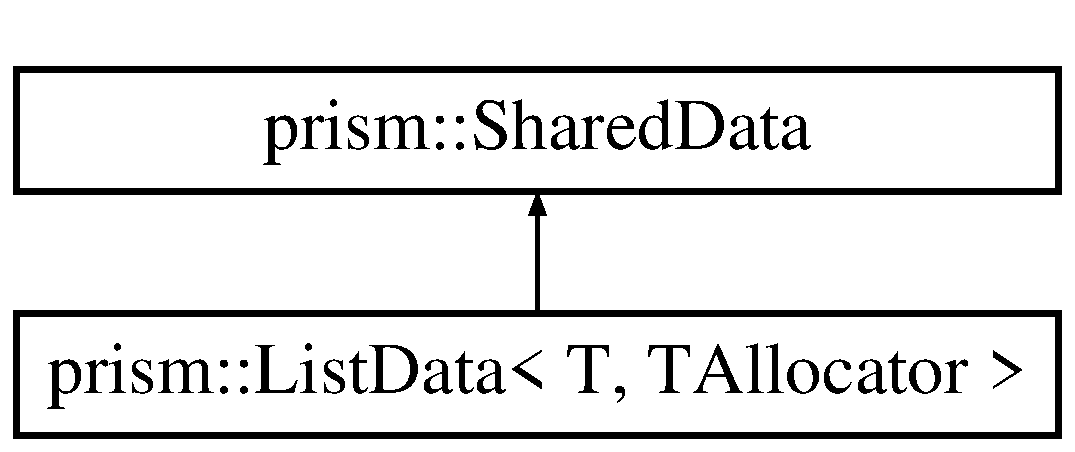
\includegraphics[height=2.000000cm]{classprism_1_1_shared_data}
\end{center}
\end{figure}
\subsection*{Public Member Functions}
\begin{DoxyCompactItemize}
\item 
\hyperlink{classprism_1_1_shared_data_a68d7aab69703ca6152731f1e041d6949}{Shared\+Data} ()
\item 
\hyperlink{classprism_1_1_shared_data_a90f3a23c943c077a2d23776ba0b207c1}{Shared\+Data} (const \hyperlink{classprism_1_1_shared_data}{Shared\+Data} \&\hyperlink{namespaceprism_ae776f4cd825f79e7af1cf6ee1d90a209}{copy})
\item 
virtual \hyperlink{classprism_1_1_shared_data_a8ededcc3f4eb86dcd47d271bd24aff0b}{$\sim$\+Shared\+Data} ()
\item 
void \hyperlink{classprism_1_1_shared_data_a270cf0cca02293714175d70acd92f049}{dec\+Ref} ()
\item 
void \hyperlink{classprism_1_1_shared_data_ae389431d573a0131b368c60531006fd2}{inc\+Ref} ()
\item 
const bool \hyperlink{classprism_1_1_shared_data_a2c995e732a31d8f9a29c2fd46e0256ff}{is\+Shareable} () const 
\item 
const bool \hyperlink{classprism_1_1_shared_data_a2b919077f094e7d8970721b77677b584}{is\+Shared} () const 
\item 
const int \hyperlink{classprism_1_1_shared_data_a4886256c18ff603dece3cad4fb4f579b}{ref\+Count} () const 
\item 
void \hyperlink{classprism_1_1_shared_data_a09445f57e7dea60a37477a36d74365ac}{set\+Unshareable} ()
\item 
\hyperlink{classprism_1_1_shared_data}{Shared\+Data} \& \hyperlink{classprism_1_1_shared_data_a0edaec2979f24e9b7c11eb80cfa630bc}{operator=} (const \hyperlink{classprism_1_1_shared_data}{Shared\+Data} \&rhs)
\end{DoxyCompactItemize}


\subsection{Constructor \& Destructor Documentation}
\index{prism\+::\+Shared\+Data@{prism\+::\+Shared\+Data}!Shared\+Data@{Shared\+Data}}
\index{Shared\+Data@{Shared\+Data}!prism\+::\+Shared\+Data@{prism\+::\+Shared\+Data}}
\subsubsection[{\texorpdfstring{Shared\+Data()}{SharedData()}}]{\setlength{\rightskip}{0pt plus 5cm}prism\+::\+Shared\+Data\+::\+Shared\+Data (
\begin{DoxyParamCaption}
{}
\end{DoxyParamCaption}
)}\hypertarget{classprism_1_1_shared_data_a68d7aab69703ca6152731f1e041d6949}{}\label{classprism_1_1_shared_data_a68d7aab69703ca6152731f1e041d6949}
\index{prism\+::\+Shared\+Data@{prism\+::\+Shared\+Data}!Shared\+Data@{Shared\+Data}}
\index{Shared\+Data@{Shared\+Data}!prism\+::\+Shared\+Data@{prism\+::\+Shared\+Data}}
\subsubsection[{\texorpdfstring{Shared\+Data(const Shared\+Data \&copy)}{SharedData(const SharedData &copy)}}]{\setlength{\rightskip}{0pt plus 5cm}prism\+::\+Shared\+Data\+::\+Shared\+Data (
\begin{DoxyParamCaption}
\item[{const {\bf Shared\+Data} \&}]{copy}
\end{DoxyParamCaption}
)}\hypertarget{classprism_1_1_shared_data_a90f3a23c943c077a2d23776ba0b207c1}{}\label{classprism_1_1_shared_data_a90f3a23c943c077a2d23776ba0b207c1}
\index{prism\+::\+Shared\+Data@{prism\+::\+Shared\+Data}!````~Shared\+Data@{$\sim$\+Shared\+Data}}
\index{````~Shared\+Data@{$\sim$\+Shared\+Data}!prism\+::\+Shared\+Data@{prism\+::\+Shared\+Data}}
\subsubsection[{\texorpdfstring{$\sim$\+Shared\+Data()}{~SharedData()}}]{\setlength{\rightskip}{0pt plus 5cm}prism\+::\+Shared\+Data\+::$\sim$\+Shared\+Data (
\begin{DoxyParamCaption}
{}
\end{DoxyParamCaption}
)\hspace{0.3cm}{\ttfamily [virtual]}}\hypertarget{classprism_1_1_shared_data_a8ededcc3f4eb86dcd47d271bd24aff0b}{}\label{classprism_1_1_shared_data_a8ededcc3f4eb86dcd47d271bd24aff0b}


\subsection{Member Function Documentation}
\index{prism\+::\+Shared\+Data@{prism\+::\+Shared\+Data}!dec\+Ref@{dec\+Ref}}
\index{dec\+Ref@{dec\+Ref}!prism\+::\+Shared\+Data@{prism\+::\+Shared\+Data}}
\subsubsection[{\texorpdfstring{dec\+Ref()}{decRef()}}]{\setlength{\rightskip}{0pt plus 5cm}void prism\+::\+Shared\+Data\+::dec\+Ref (
\begin{DoxyParamCaption}
{}
\end{DoxyParamCaption}
)}\hypertarget{classprism_1_1_shared_data_a270cf0cca02293714175d70acd92f049}{}\label{classprism_1_1_shared_data_a270cf0cca02293714175d70acd92f049}
\index{prism\+::\+Shared\+Data@{prism\+::\+Shared\+Data}!inc\+Ref@{inc\+Ref}}
\index{inc\+Ref@{inc\+Ref}!prism\+::\+Shared\+Data@{prism\+::\+Shared\+Data}}
\subsubsection[{\texorpdfstring{inc\+Ref()}{incRef()}}]{\setlength{\rightskip}{0pt plus 5cm}void prism\+::\+Shared\+Data\+::inc\+Ref (
\begin{DoxyParamCaption}
{}
\end{DoxyParamCaption}
)}\hypertarget{classprism_1_1_shared_data_ae389431d573a0131b368c60531006fd2}{}\label{classprism_1_1_shared_data_ae389431d573a0131b368c60531006fd2}
\index{prism\+::\+Shared\+Data@{prism\+::\+Shared\+Data}!is\+Shareable@{is\+Shareable}}
\index{is\+Shareable@{is\+Shareable}!prism\+::\+Shared\+Data@{prism\+::\+Shared\+Data}}
\subsubsection[{\texorpdfstring{is\+Shareable() const }{isShareable() const }}]{\setlength{\rightskip}{0pt plus 5cm}const bool prism\+::\+Shared\+Data\+::is\+Shareable (
\begin{DoxyParamCaption}
{}
\end{DoxyParamCaption}
) const}\hypertarget{classprism_1_1_shared_data_a2c995e732a31d8f9a29c2fd46e0256ff}{}\label{classprism_1_1_shared_data_a2c995e732a31d8f9a29c2fd46e0256ff}
\index{prism\+::\+Shared\+Data@{prism\+::\+Shared\+Data}!is\+Shared@{is\+Shared}}
\index{is\+Shared@{is\+Shared}!prism\+::\+Shared\+Data@{prism\+::\+Shared\+Data}}
\subsubsection[{\texorpdfstring{is\+Shared() const }{isShared() const }}]{\setlength{\rightskip}{0pt plus 5cm}const bool prism\+::\+Shared\+Data\+::is\+Shared (
\begin{DoxyParamCaption}
{}
\end{DoxyParamCaption}
) const}\hypertarget{classprism_1_1_shared_data_a2b919077f094e7d8970721b77677b584}{}\label{classprism_1_1_shared_data_a2b919077f094e7d8970721b77677b584}
\index{prism\+::\+Shared\+Data@{prism\+::\+Shared\+Data}!operator=@{operator=}}
\index{operator=@{operator=}!prism\+::\+Shared\+Data@{prism\+::\+Shared\+Data}}
\subsubsection[{\texorpdfstring{operator=(const Shared\+Data \&rhs)}{operator=(const SharedData &rhs)}}]{\setlength{\rightskip}{0pt plus 5cm}{\bf Shared\+Data} \& prism\+::\+Shared\+Data\+::operator= (
\begin{DoxyParamCaption}
\item[{const {\bf Shared\+Data} \&}]{rhs}
\end{DoxyParamCaption}
)}\hypertarget{classprism_1_1_shared_data_a0edaec2979f24e9b7c11eb80cfa630bc}{}\label{classprism_1_1_shared_data_a0edaec2979f24e9b7c11eb80cfa630bc}
\index{prism\+::\+Shared\+Data@{prism\+::\+Shared\+Data}!ref\+Count@{ref\+Count}}
\index{ref\+Count@{ref\+Count}!prism\+::\+Shared\+Data@{prism\+::\+Shared\+Data}}
\subsubsection[{\texorpdfstring{ref\+Count() const }{refCount() const }}]{\setlength{\rightskip}{0pt plus 5cm}const int prism\+::\+Shared\+Data\+::ref\+Count (
\begin{DoxyParamCaption}
{}
\end{DoxyParamCaption}
) const}\hypertarget{classprism_1_1_shared_data_a4886256c18ff603dece3cad4fb4f579b}{}\label{classprism_1_1_shared_data_a4886256c18ff603dece3cad4fb4f579b}
\index{prism\+::\+Shared\+Data@{prism\+::\+Shared\+Data}!set\+Unshareable@{set\+Unshareable}}
\index{set\+Unshareable@{set\+Unshareable}!prism\+::\+Shared\+Data@{prism\+::\+Shared\+Data}}
\subsubsection[{\texorpdfstring{set\+Unshareable()}{setUnshareable()}}]{\setlength{\rightskip}{0pt plus 5cm}void prism\+::\+Shared\+Data\+::set\+Unshareable (
\begin{DoxyParamCaption}
{}
\end{DoxyParamCaption}
)}\hypertarget{classprism_1_1_shared_data_a09445f57e7dea60a37477a36d74365ac}{}\label{classprism_1_1_shared_data_a09445f57e7dea60a37477a36d74365ac}


The documentation for this class was generated from the following files\+:\begin{DoxyCompactItemize}
\item 
inc/prism/h/\hyperlink{_shared_data_8h}{Shared\+Data.\+h}\item 
src/prism/\hyperlink{_shared_data_8cpp}{Shared\+Data.\+cpp}\end{DoxyCompactItemize}

\hypertarget{classprism_1_1_shared_data_pointer}{}\section{prism\+:\+:Shared\+Data\+Pointer$<$ Shared\+Data\+Type $>$ Class Template Reference}
\label{classprism_1_1_shared_data_pointer}\index{prism\+::\+Shared\+Data\+Pointer$<$ Shared\+Data\+Type $>$@{prism\+::\+Shared\+Data\+Pointer$<$ Shared\+Data\+Type $>$}}
\subsection*{Public Member Functions}
\begin{DoxyCompactItemize}
\item 
\hyperlink{classprism_1_1_shared_data_pointer_aae89ba1520cd16d5d6efc06c3c763a57}{Shared\+Data\+Pointer} ()
\item 
\hyperlink{classprism_1_1_shared_data_pointer_a8f33e2be524ada8415b31533876f7a4d}{Shared\+Data\+Pointer} (Shared\+Data\+Type $\ast$p)
\item 
\hyperlink{classprism_1_1_shared_data_pointer_a3e8fb06e78156d0341984e8ef4002f6e}{Shared\+Data\+Pointer} (const \hyperlink{classprism_1_1_shared_data_pointer}{Shared\+Data\+Pointer} \&\hyperlink{namespaceprism_ae776f4cd825f79e7af1cf6ee1d90a209}{copy})
\item 
\hyperlink{classprism_1_1_shared_data_pointer}{Shared\+Data\+Pointer} \& \hyperlink{classprism_1_1_shared_data_pointer_a1e683956ccbe47d262c92f934d04f254}{operator=} (const \hyperlink{classprism_1_1_shared_data_pointer}{Shared\+Data\+Pointer} \&rhs)
\item 
\hyperlink{classprism_1_1_shared_data_pointer_a0c2b49901e71a8d43a0b34685653032c}{$\sim$\+Shared\+Data\+Pointer} ()
\item 
const Shared\+Data\+Type $\ast$ \hyperlink{classprism_1_1_shared_data_pointer_a4748e8c520ac7cc9d73d2c763cbad7fb}{const\+Data} () const 
\item 
Shared\+Data\+Type $\ast$ \hyperlink{classprism_1_1_shared_data_pointer_ae0acea5732c353a5ce4afb54c07e7302}{data} ()
\item 
const Shared\+Data\+Type $\ast$ \hyperlink{classprism_1_1_shared_data_pointer_a2d6b477eed9cb60c0197cce0361f37cd}{data} () const 
\item 
void \hyperlink{classprism_1_1_shared_data_pointer_aa222b261cf3a1ef3c36affa1ae6eda3a}{detach} ()
\item 
const bool \hyperlink{classprism_1_1_shared_data_pointer_a2791e89091e965f1d06f2986ee05d810}{is\+Null} () const 
\item 
const bool \hyperlink{classprism_1_1_shared_data_pointer_a6b23c069510ae95130c6ecbca454b054}{is\+Shareable} () const 
\item 
const bool \hyperlink{classprism_1_1_shared_data_pointer_ace1d2a6b6563102b321f091729290f33}{is\+Shared} () const 
\item 
const int \hyperlink{classprism_1_1_shared_data_pointer_aec5ca29b4604c039d7fecdead3b03db4}{ref\+Count} () const 
\item 
void \hyperlink{classprism_1_1_shared_data_pointer_af2c4b48383be86e85cb46864ddae768f}{set\+Unshareable} ()
\item 
Shared\+Data\+Type $\ast$ \hyperlink{classprism_1_1_shared_data_pointer_acc512f07fead7332f920071177cad7bb}{operator-\/$>$} ()
\item 
const Shared\+Data\+Type $\ast$ \hyperlink{classprism_1_1_shared_data_pointer_ad107d76166d80cbcd3894533dc7b7be5}{operator-\/$>$} () const 
\item 
Shared\+Data\+Type \& \hyperlink{classprism_1_1_shared_data_pointer_a225343b932084283c498f666a10de3ec}{operator$\ast$} ()
\item 
const Shared\+Data\+Type \& \hyperlink{classprism_1_1_shared_data_pointer_adb8f9ef44184f78552bbfba9e55e7fc5}{operator$\ast$} () const 
\item 
const bool \hyperlink{classprism_1_1_shared_data_pointer_afdfedb3de13176fdc9d7bb8fce20ee9a}{operator!} () const 
\item 
const bool \hyperlink{classprism_1_1_shared_data_pointer_a1a793e8c8410d0a979b0269e071fa82a}{operator!=} (const \hyperlink{classprism_1_1_shared_data_pointer}{Shared\+Data\+Pointer} \&rhs) const 
\item 
const bool \hyperlink{classprism_1_1_shared_data_pointer_ab9603e8d447ca8968d06b29f056110f9}{operator==} (const \hyperlink{classprism_1_1_shared_data_pointer}{Shared\+Data\+Pointer}$<$ Shared\+Data\+Type $>$ \&rhs) const 
\end{DoxyCompactItemize}


\subsection{Constructor \& Destructor Documentation}
\index{prism\+::\+Shared\+Data\+Pointer@{prism\+::\+Shared\+Data\+Pointer}!Shared\+Data\+Pointer@{Shared\+Data\+Pointer}}
\index{Shared\+Data\+Pointer@{Shared\+Data\+Pointer}!prism\+::\+Shared\+Data\+Pointer@{prism\+::\+Shared\+Data\+Pointer}}
\subsubsection[{\texorpdfstring{Shared\+Data\+Pointer()}{SharedDataPointer()}}]{\setlength{\rightskip}{0pt plus 5cm}template$<$class Shared\+Data\+Type $>$ {\bf prism\+::\+Shared\+Data\+Pointer}$<$ Shared\+Data\+Type $>$\+::{\bf Shared\+Data\+Pointer} (
\begin{DoxyParamCaption}
{}
\end{DoxyParamCaption}
)\hspace{0.3cm}{\ttfamily [inline]}}\hypertarget{classprism_1_1_shared_data_pointer_aae89ba1520cd16d5d6efc06c3c763a57}{}\label{classprism_1_1_shared_data_pointer_aae89ba1520cd16d5d6efc06c3c763a57}
\index{prism\+::\+Shared\+Data\+Pointer@{prism\+::\+Shared\+Data\+Pointer}!Shared\+Data\+Pointer@{Shared\+Data\+Pointer}}
\index{Shared\+Data\+Pointer@{Shared\+Data\+Pointer}!prism\+::\+Shared\+Data\+Pointer@{prism\+::\+Shared\+Data\+Pointer}}
\subsubsection[{\texorpdfstring{Shared\+Data\+Pointer(\+Shared\+Data\+Type $\ast$p)}{SharedDataPointer(SharedDataType *p)}}]{\setlength{\rightskip}{0pt plus 5cm}template$<$class Shared\+Data\+Type$>$ {\bf prism\+::\+Shared\+Data\+Pointer}$<$ Shared\+Data\+Type $>$\+::{\bf Shared\+Data\+Pointer} (
\begin{DoxyParamCaption}
\item[{Shared\+Data\+Type $\ast$}]{p}
\end{DoxyParamCaption}
)\hspace{0.3cm}{\ttfamily [inline]}}\hypertarget{classprism_1_1_shared_data_pointer_a8f33e2be524ada8415b31533876f7a4d}{}\label{classprism_1_1_shared_data_pointer_a8f33e2be524ada8415b31533876f7a4d}
\index{prism\+::\+Shared\+Data\+Pointer@{prism\+::\+Shared\+Data\+Pointer}!Shared\+Data\+Pointer@{Shared\+Data\+Pointer}}
\index{Shared\+Data\+Pointer@{Shared\+Data\+Pointer}!prism\+::\+Shared\+Data\+Pointer@{prism\+::\+Shared\+Data\+Pointer}}
\subsubsection[{\texorpdfstring{Shared\+Data\+Pointer(const Shared\+Data\+Pointer \&copy)}{SharedDataPointer(const SharedDataPointer &copy)}}]{\setlength{\rightskip}{0pt plus 5cm}template$<$class Shared\+Data\+Type$>$ {\bf prism\+::\+Shared\+Data\+Pointer}$<$ Shared\+Data\+Type $>$\+::{\bf Shared\+Data\+Pointer} (
\begin{DoxyParamCaption}
\item[{const {\bf Shared\+Data\+Pointer}$<$ Shared\+Data\+Type $>$ \&}]{copy}
\end{DoxyParamCaption}
)\hspace{0.3cm}{\ttfamily [inline]}}\hypertarget{classprism_1_1_shared_data_pointer_a3e8fb06e78156d0341984e8ef4002f6e}{}\label{classprism_1_1_shared_data_pointer_a3e8fb06e78156d0341984e8ef4002f6e}
\index{prism\+::\+Shared\+Data\+Pointer@{prism\+::\+Shared\+Data\+Pointer}!````~Shared\+Data\+Pointer@{$\sim$\+Shared\+Data\+Pointer}}
\index{````~Shared\+Data\+Pointer@{$\sim$\+Shared\+Data\+Pointer}!prism\+::\+Shared\+Data\+Pointer@{prism\+::\+Shared\+Data\+Pointer}}
\subsubsection[{\texorpdfstring{$\sim$\+Shared\+Data\+Pointer()}{~SharedDataPointer()}}]{\setlength{\rightskip}{0pt plus 5cm}template$<$class Shared\+Data\+Type $>$ {\bf prism\+::\+Shared\+Data\+Pointer}$<$ Shared\+Data\+Type $>$\+::$\sim${\bf Shared\+Data\+Pointer} (
\begin{DoxyParamCaption}
{}
\end{DoxyParamCaption}
)\hspace{0.3cm}{\ttfamily [inline]}}\hypertarget{classprism_1_1_shared_data_pointer_a0c2b49901e71a8d43a0b34685653032c}{}\label{classprism_1_1_shared_data_pointer_a0c2b49901e71a8d43a0b34685653032c}


\subsection{Member Function Documentation}
\index{prism\+::\+Shared\+Data\+Pointer@{prism\+::\+Shared\+Data\+Pointer}!const\+Data@{const\+Data}}
\index{const\+Data@{const\+Data}!prism\+::\+Shared\+Data\+Pointer@{prism\+::\+Shared\+Data\+Pointer}}
\subsubsection[{\texorpdfstring{const\+Data() const }{constData() const }}]{\setlength{\rightskip}{0pt plus 5cm}template$<$class Shared\+Data\+Type $>$ const Shared\+Data\+Type $\ast$ {\bf prism\+::\+Shared\+Data\+Pointer}$<$ Shared\+Data\+Type $>$\+::const\+Data (
\begin{DoxyParamCaption}
{}
\end{DoxyParamCaption}
) const\hspace{0.3cm}{\ttfamily [inline]}}\hypertarget{classprism_1_1_shared_data_pointer_a4748e8c520ac7cc9d73d2c763cbad7fb}{}\label{classprism_1_1_shared_data_pointer_a4748e8c520ac7cc9d73d2c763cbad7fb}
\index{prism\+::\+Shared\+Data\+Pointer@{prism\+::\+Shared\+Data\+Pointer}!data@{data}}
\index{data@{data}!prism\+::\+Shared\+Data\+Pointer@{prism\+::\+Shared\+Data\+Pointer}}
\subsubsection[{\texorpdfstring{data()}{data()}}]{\setlength{\rightskip}{0pt plus 5cm}template$<$class Shared\+Data\+Type $>$ Shared\+Data\+Type $\ast$ {\bf prism\+::\+Shared\+Data\+Pointer}$<$ Shared\+Data\+Type $>$\+::data (
\begin{DoxyParamCaption}
{}
\end{DoxyParamCaption}
)\hspace{0.3cm}{\ttfamily [inline]}}\hypertarget{classprism_1_1_shared_data_pointer_ae0acea5732c353a5ce4afb54c07e7302}{}\label{classprism_1_1_shared_data_pointer_ae0acea5732c353a5ce4afb54c07e7302}
\index{prism\+::\+Shared\+Data\+Pointer@{prism\+::\+Shared\+Data\+Pointer}!data@{data}}
\index{data@{data}!prism\+::\+Shared\+Data\+Pointer@{prism\+::\+Shared\+Data\+Pointer}}
\subsubsection[{\texorpdfstring{data() const }{data() const }}]{\setlength{\rightskip}{0pt plus 5cm}template$<$class Shared\+Data\+Type $>$ const Shared\+Data\+Type $\ast$ {\bf prism\+::\+Shared\+Data\+Pointer}$<$ Shared\+Data\+Type $>$\+::data (
\begin{DoxyParamCaption}
{}
\end{DoxyParamCaption}
) const\hspace{0.3cm}{\ttfamily [inline]}}\hypertarget{classprism_1_1_shared_data_pointer_a2d6b477eed9cb60c0197cce0361f37cd}{}\label{classprism_1_1_shared_data_pointer_a2d6b477eed9cb60c0197cce0361f37cd}
\index{prism\+::\+Shared\+Data\+Pointer@{prism\+::\+Shared\+Data\+Pointer}!detach@{detach}}
\index{detach@{detach}!prism\+::\+Shared\+Data\+Pointer@{prism\+::\+Shared\+Data\+Pointer}}
\subsubsection[{\texorpdfstring{detach()}{detach()}}]{\setlength{\rightskip}{0pt plus 5cm}template$<$typename Shared\+Data\+Type $>$ void {\bf prism\+::\+Shared\+Data\+Pointer}$<$ Shared\+Data\+Type $>$\+::detach (
\begin{DoxyParamCaption}
{}
\end{DoxyParamCaption}
)\hspace{0.3cm}{\ttfamily [inline]}}\hypertarget{classprism_1_1_shared_data_pointer_aa222b261cf3a1ef3c36affa1ae6eda3a}{}\label{classprism_1_1_shared_data_pointer_aa222b261cf3a1ef3c36affa1ae6eda3a}
\index{prism\+::\+Shared\+Data\+Pointer@{prism\+::\+Shared\+Data\+Pointer}!is\+Null@{is\+Null}}
\index{is\+Null@{is\+Null}!prism\+::\+Shared\+Data\+Pointer@{prism\+::\+Shared\+Data\+Pointer}}
\subsubsection[{\texorpdfstring{is\+Null() const }{isNull() const }}]{\setlength{\rightskip}{0pt plus 5cm}template$<$class Shared\+Data\+Type $>$ const bool {\bf prism\+::\+Shared\+Data\+Pointer}$<$ Shared\+Data\+Type $>$\+::is\+Null (
\begin{DoxyParamCaption}
{}
\end{DoxyParamCaption}
) const\hspace{0.3cm}{\ttfamily [inline]}}\hypertarget{classprism_1_1_shared_data_pointer_a2791e89091e965f1d06f2986ee05d810}{}\label{classprism_1_1_shared_data_pointer_a2791e89091e965f1d06f2986ee05d810}
\index{prism\+::\+Shared\+Data\+Pointer@{prism\+::\+Shared\+Data\+Pointer}!is\+Shareable@{is\+Shareable}}
\index{is\+Shareable@{is\+Shareable}!prism\+::\+Shared\+Data\+Pointer@{prism\+::\+Shared\+Data\+Pointer}}
\subsubsection[{\texorpdfstring{is\+Shareable() const }{isShareable() const }}]{\setlength{\rightskip}{0pt plus 5cm}template$<$typename Shared\+Data\+Type $>$ const bool {\bf prism\+::\+Shared\+Data\+Pointer}$<$ Shared\+Data\+Type $>$\+::is\+Shareable (
\begin{DoxyParamCaption}
{}
\end{DoxyParamCaption}
) const\hspace{0.3cm}{\ttfamily [inline]}}\hypertarget{classprism_1_1_shared_data_pointer_a6b23c069510ae95130c6ecbca454b054}{}\label{classprism_1_1_shared_data_pointer_a6b23c069510ae95130c6ecbca454b054}
\index{prism\+::\+Shared\+Data\+Pointer@{prism\+::\+Shared\+Data\+Pointer}!is\+Shared@{is\+Shared}}
\index{is\+Shared@{is\+Shared}!prism\+::\+Shared\+Data\+Pointer@{prism\+::\+Shared\+Data\+Pointer}}
\subsubsection[{\texorpdfstring{is\+Shared() const }{isShared() const }}]{\setlength{\rightskip}{0pt plus 5cm}template$<$typename Shared\+Data\+Type $>$ const bool {\bf prism\+::\+Shared\+Data\+Pointer}$<$ Shared\+Data\+Type $>$\+::is\+Shared (
\begin{DoxyParamCaption}
{}
\end{DoxyParamCaption}
) const\hspace{0.3cm}{\ttfamily [inline]}}\hypertarget{classprism_1_1_shared_data_pointer_ace1d2a6b6563102b321f091729290f33}{}\label{classprism_1_1_shared_data_pointer_ace1d2a6b6563102b321f091729290f33}
\index{prism\+::\+Shared\+Data\+Pointer@{prism\+::\+Shared\+Data\+Pointer}!operator"!@{operator"!}}
\index{operator"!@{operator"!}!prism\+::\+Shared\+Data\+Pointer@{prism\+::\+Shared\+Data\+Pointer}}
\subsubsection[{\texorpdfstring{operator"!() const }{operator!() const }}]{\setlength{\rightskip}{0pt plus 5cm}template$<$class Shared\+Data\+Type $>$ const bool {\bf prism\+::\+Shared\+Data\+Pointer}$<$ Shared\+Data\+Type $>$\+::operator! (
\begin{DoxyParamCaption}
{}
\end{DoxyParamCaption}
) const\hspace{0.3cm}{\ttfamily [inline]}}\hypertarget{classprism_1_1_shared_data_pointer_afdfedb3de13176fdc9d7bb8fce20ee9a}{}\label{classprism_1_1_shared_data_pointer_afdfedb3de13176fdc9d7bb8fce20ee9a}
\index{prism\+::\+Shared\+Data\+Pointer@{prism\+::\+Shared\+Data\+Pointer}!operator"!=@{operator"!=}}
\index{operator"!=@{operator"!=}!prism\+::\+Shared\+Data\+Pointer@{prism\+::\+Shared\+Data\+Pointer}}
\subsubsection[{\texorpdfstring{operator"!=(const Shared\+Data\+Pointer \&rhs) const }{operator!=(const SharedDataPointer &rhs) const }}]{\setlength{\rightskip}{0pt plus 5cm}template$<$class Shared\+Data\+Type $>$ const bool {\bf prism\+::\+Shared\+Data\+Pointer}$<$ Shared\+Data\+Type $>$\+::{\bf operator!}= (
\begin{DoxyParamCaption}
\item[{const {\bf Shared\+Data\+Pointer}$<$ Shared\+Data\+Type $>$ \&}]{rhs}
\end{DoxyParamCaption}
) const\hspace{0.3cm}{\ttfamily [inline]}}\hypertarget{classprism_1_1_shared_data_pointer_a1a793e8c8410d0a979b0269e071fa82a}{}\label{classprism_1_1_shared_data_pointer_a1a793e8c8410d0a979b0269e071fa82a}
\index{prism\+::\+Shared\+Data\+Pointer@{prism\+::\+Shared\+Data\+Pointer}!operator$\ast$@{operator$\ast$}}
\index{operator$\ast$@{operator$\ast$}!prism\+::\+Shared\+Data\+Pointer@{prism\+::\+Shared\+Data\+Pointer}}
\subsubsection[{\texorpdfstring{operator$\ast$()}{operator*()}}]{\setlength{\rightskip}{0pt plus 5cm}template$<$class Shared\+Data\+Type $>$ Shared\+Data\+Type \& {\bf prism\+::\+Shared\+Data\+Pointer}$<$ Shared\+Data\+Type $>$\+::operator$\ast$ (
\begin{DoxyParamCaption}
{}
\end{DoxyParamCaption}
)\hspace{0.3cm}{\ttfamily [inline]}}\hypertarget{classprism_1_1_shared_data_pointer_a225343b932084283c498f666a10de3ec}{}\label{classprism_1_1_shared_data_pointer_a225343b932084283c498f666a10de3ec}
\index{prism\+::\+Shared\+Data\+Pointer@{prism\+::\+Shared\+Data\+Pointer}!operator$\ast$@{operator$\ast$}}
\index{operator$\ast$@{operator$\ast$}!prism\+::\+Shared\+Data\+Pointer@{prism\+::\+Shared\+Data\+Pointer}}
\subsubsection[{\texorpdfstring{operator$\ast$() const }{operator*() const }}]{\setlength{\rightskip}{0pt plus 5cm}template$<$class Shared\+Data\+Type $>$ const Shared\+Data\+Type \& {\bf prism\+::\+Shared\+Data\+Pointer}$<$ Shared\+Data\+Type $>$\+::operator$\ast$ (
\begin{DoxyParamCaption}
{}
\end{DoxyParamCaption}
) const\hspace{0.3cm}{\ttfamily [inline]}}\hypertarget{classprism_1_1_shared_data_pointer_adb8f9ef44184f78552bbfba9e55e7fc5}{}\label{classprism_1_1_shared_data_pointer_adb8f9ef44184f78552bbfba9e55e7fc5}
\index{prism\+::\+Shared\+Data\+Pointer@{prism\+::\+Shared\+Data\+Pointer}!operator-\/$>$@{operator-\/$>$}}
\index{operator-\/$>$@{operator-\/$>$}!prism\+::\+Shared\+Data\+Pointer@{prism\+::\+Shared\+Data\+Pointer}}
\subsubsection[{\texorpdfstring{operator-\/$>$()}{operator->()}}]{\setlength{\rightskip}{0pt plus 5cm}template$<$class Shared\+Data\+Type $>$ Shared\+Data\+Type $\ast$ {\bf prism\+::\+Shared\+Data\+Pointer}$<$ Shared\+Data\+Type $>$\+::operator-\/$>$ (
\begin{DoxyParamCaption}
{}
\end{DoxyParamCaption}
)\hspace{0.3cm}{\ttfamily [inline]}}\hypertarget{classprism_1_1_shared_data_pointer_acc512f07fead7332f920071177cad7bb}{}\label{classprism_1_1_shared_data_pointer_acc512f07fead7332f920071177cad7bb}
\index{prism\+::\+Shared\+Data\+Pointer@{prism\+::\+Shared\+Data\+Pointer}!operator-\/$>$@{operator-\/$>$}}
\index{operator-\/$>$@{operator-\/$>$}!prism\+::\+Shared\+Data\+Pointer@{prism\+::\+Shared\+Data\+Pointer}}
\subsubsection[{\texorpdfstring{operator-\/$>$() const }{operator->() const }}]{\setlength{\rightskip}{0pt plus 5cm}template$<$class Shared\+Data\+Type $>$ const Shared\+Data\+Type $\ast$ {\bf prism\+::\+Shared\+Data\+Pointer}$<$ Shared\+Data\+Type $>$\+::operator-\/$>$ (
\begin{DoxyParamCaption}
{}
\end{DoxyParamCaption}
) const\hspace{0.3cm}{\ttfamily [inline]}}\hypertarget{classprism_1_1_shared_data_pointer_ad107d76166d80cbcd3894533dc7b7be5}{}\label{classprism_1_1_shared_data_pointer_ad107d76166d80cbcd3894533dc7b7be5}
\index{prism\+::\+Shared\+Data\+Pointer@{prism\+::\+Shared\+Data\+Pointer}!operator=@{operator=}}
\index{operator=@{operator=}!prism\+::\+Shared\+Data\+Pointer@{prism\+::\+Shared\+Data\+Pointer}}
\subsubsection[{\texorpdfstring{operator=(const Shared\+Data\+Pointer \&rhs)}{operator=(const SharedDataPointer &rhs)}}]{\setlength{\rightskip}{0pt plus 5cm}template$<$class Shared\+Data\+Type $>$ {\bf Shared\+Data\+Pointer}$<$ Shared\+Data\+Type $>$ \& {\bf prism\+::\+Shared\+Data\+Pointer}$<$ Shared\+Data\+Type $>$\+::operator= (
\begin{DoxyParamCaption}
\item[{const {\bf Shared\+Data\+Pointer}$<$ Shared\+Data\+Type $>$ \&}]{rhs}
\end{DoxyParamCaption}
)\hspace{0.3cm}{\ttfamily [inline]}}\hypertarget{classprism_1_1_shared_data_pointer_a1e683956ccbe47d262c92f934d04f254}{}\label{classprism_1_1_shared_data_pointer_a1e683956ccbe47d262c92f934d04f254}
\index{prism\+::\+Shared\+Data\+Pointer@{prism\+::\+Shared\+Data\+Pointer}!operator==@{operator==}}
\index{operator==@{operator==}!prism\+::\+Shared\+Data\+Pointer@{prism\+::\+Shared\+Data\+Pointer}}
\subsubsection[{\texorpdfstring{operator==(const Shared\+Data\+Pointer$<$ Shared\+Data\+Type $>$ \&rhs) const }{operator==(const SharedDataPointer< SharedDataType > &rhs) const }}]{\setlength{\rightskip}{0pt plus 5cm}template$<$class Shared\+Data\+Type$>$ const bool {\bf prism\+::\+Shared\+Data\+Pointer}$<$ Shared\+Data\+Type $>$\+::operator== (
\begin{DoxyParamCaption}
\item[{const {\bf Shared\+Data\+Pointer}$<$ Shared\+Data\+Type $>$ \&}]{rhs}
\end{DoxyParamCaption}
) const\hspace{0.3cm}{\ttfamily [inline]}}\hypertarget{classprism_1_1_shared_data_pointer_ab9603e8d447ca8968d06b29f056110f9}{}\label{classprism_1_1_shared_data_pointer_ab9603e8d447ca8968d06b29f056110f9}
\index{prism\+::\+Shared\+Data\+Pointer@{prism\+::\+Shared\+Data\+Pointer}!ref\+Count@{ref\+Count}}
\index{ref\+Count@{ref\+Count}!prism\+::\+Shared\+Data\+Pointer@{prism\+::\+Shared\+Data\+Pointer}}
\subsubsection[{\texorpdfstring{ref\+Count() const }{refCount() const }}]{\setlength{\rightskip}{0pt plus 5cm}template$<$class Shared\+Data\+Type $>$ const int {\bf prism\+::\+Shared\+Data\+Pointer}$<$ Shared\+Data\+Type $>$\+::ref\+Count (
\begin{DoxyParamCaption}
{}
\end{DoxyParamCaption}
) const\hspace{0.3cm}{\ttfamily [inline]}}\hypertarget{classprism_1_1_shared_data_pointer_aec5ca29b4604c039d7fecdead3b03db4}{}\label{classprism_1_1_shared_data_pointer_aec5ca29b4604c039d7fecdead3b03db4}
\index{prism\+::\+Shared\+Data\+Pointer@{prism\+::\+Shared\+Data\+Pointer}!set\+Unshareable@{set\+Unshareable}}
\index{set\+Unshareable@{set\+Unshareable}!prism\+::\+Shared\+Data\+Pointer@{prism\+::\+Shared\+Data\+Pointer}}
\subsubsection[{\texorpdfstring{set\+Unshareable()}{setUnshareable()}}]{\setlength{\rightskip}{0pt plus 5cm}template$<$typename Shared\+Data\+Type $>$ void {\bf prism\+::\+Shared\+Data\+Pointer}$<$ Shared\+Data\+Type $>$\+::set\+Unshareable (
\begin{DoxyParamCaption}
{}
\end{DoxyParamCaption}
)\hspace{0.3cm}{\ttfamily [inline]}}\hypertarget{classprism_1_1_shared_data_pointer_af2c4b48383be86e85cb46864ddae768f}{}\label{classprism_1_1_shared_data_pointer_af2c4b48383be86e85cb46864ddae768f}


The documentation for this class was generated from the following file\+:\begin{DoxyCompactItemize}
\item 
\hyperlink{_shared_data_pointer_8h}{Shared\+Data\+Pointer.\+h}\end{DoxyCompactItemize}

\hypertarget{classprism_1_1_shared_pointer}{}\section{prism\+:\+:Shared\+Pointer$<$ T $>$ Class Template Reference}
\label{classprism_1_1_shared_pointer}\index{prism\+::\+Shared\+Pointer$<$ T $>$@{prism\+::\+Shared\+Pointer$<$ T $>$}}
\subsection*{Public Member Functions}
\begin{DoxyCompactItemize}
\item 
\hyperlink{classprism_1_1_shared_pointer_a076711618f299e5a5d04261d7d806aff}{Shared\+Pointer} ()
\item 
\hyperlink{classprism_1_1_shared_pointer_a0b8d1327178383b39bd6bb2826d384b4}{Shared\+Pointer} (T $\ast$\hyperlink{classprism_1_1_shared_pointer_aecf5f8614d4c5683e6c0207436ed8900}{data})
\item 
\hyperlink{classprism_1_1_shared_pointer_a7346c06b6c0e7c80236472c4d085460c}{Shared\+Pointer} (const \hyperlink{classprism_1_1_shared_pointer}{Shared\+Pointer}$<$ T $>$ \&\hyperlink{namespaceprism_ae776f4cd825f79e7af1cf6ee1d90a209}{copy})
\item 
\hyperlink{classprism_1_1_shared_pointer_a9892f1a766b66491af8a7356cb574ac3}{$\sim$\+Shared\+Pointer} ()
\item 
void \hyperlink{classprism_1_1_shared_pointer_a70f571a23e5c800d43f309cea9857360}{clear} ()
\item 
T $\ast$ \hyperlink{classprism_1_1_shared_pointer_aecf5f8614d4c5683e6c0207436ed8900}{data} () const 
\item 
const bool \hyperlink{classprism_1_1_shared_pointer_a011b5c5b151717cfcc45bce7eb969254}{is\+Null} () const 
\item 
const bool \hyperlink{classprism_1_1_shared_pointer_ad0eef18b3e5c37274f22cff8b88f7d66}{is\+Unique} () const 
\item 
const int \hyperlink{classprism_1_1_shared_pointer_a6b122ff924644d334ae0ff9f184af047}{ref\+Count} () const 
\item 
T $\ast$ \hyperlink{classprism_1_1_shared_pointer_a46555958394709490c4e7378c7bd2a39}{operator-\/$>$} () const 
\item 
T \& \hyperlink{classprism_1_1_shared_pointer_aef4f7418cd76f2a7b0cb20ad83e44720}{operator$\ast$} () const 
\item 
\hyperlink{classprism_1_1_shared_pointer_a1d05fe8cac7da2ea12fc321c45f59391}{operator bool} () const 
\item 
const bool \hyperlink{classprism_1_1_shared_pointer_a6a9e94b71b5ead6c0edbc836e3babb74}{operator!} () const 
\item 
\hyperlink{classprism_1_1_shared_pointer}{Shared\+Pointer} \& \hyperlink{classprism_1_1_shared_pointer_a1cc6ec5d911e2f86c2bfe07be115cd1e}{operator=} (const \hyperlink{classprism_1_1_shared_pointer}{Shared\+Pointer} \&rhs)
\end{DoxyCompactItemize}
\subsection*{Friends}
\begin{DoxyCompactItemize}
\item 
{\footnotesize template$<$class U $>$ }\\const bool \hyperlink{classprism_1_1_shared_pointer_a497bc2f2bc9e68da0cd9a80dc5b3b99a}{operator!=} (const \hyperlink{classprism_1_1_shared_pointer}{Shared\+Pointer}$<$ U $>$ \&p1, const \hyperlink{classprism_1_1_shared_pointer}{Shared\+Pointer}$<$ U $>$ \&p2)
\item 
{\footnotesize template$<$class U $>$ }\\const bool \hyperlink{classprism_1_1_shared_pointer_afa1e95ed17f645ed02ee12494d006a7b}{operator!=} (const \hyperlink{classprism_1_1_shared_pointer}{Shared\+Pointer}$<$ U $>$ \&p1, const U $\ast$p2)
\item 
{\footnotesize template$<$class U $>$ }\\const bool \hyperlink{classprism_1_1_shared_pointer_a6e788a3f86ea0f744f7f58ff0d1a6365}{operator!=} (const U $\ast$p1, const \hyperlink{classprism_1_1_shared_pointer}{Shared\+Pointer}$<$ U $>$ \&p2)
\item 
{\footnotesize template$<$class U $>$ }\\const bool \hyperlink{classprism_1_1_shared_pointer_ae1688caf7bd4dc08f775cbe830ecd6cd}{operator==} (const \hyperlink{classprism_1_1_shared_pointer}{Shared\+Pointer}$<$ U $>$ \&p1, const \hyperlink{classprism_1_1_shared_pointer}{Shared\+Pointer}$<$ U $>$ \&p2)
\item 
{\footnotesize template$<$class U $>$ }\\const bool \hyperlink{classprism_1_1_shared_pointer_ac396e2d37f10207b0e4da099d03ef759}{operator==} (const \hyperlink{classprism_1_1_shared_pointer}{Shared\+Pointer}$<$ U $>$ \&p1, const U $\ast$p2)
\item 
{\footnotesize template$<$class U $>$ }\\const bool \hyperlink{classprism_1_1_shared_pointer_a4001c70f47a8e58a039f8f657f8334b5}{operator==} (const U $\ast$p1, const \hyperlink{classprism_1_1_shared_pointer}{Shared\+Pointer}$<$ U $>$ \&p2)
\item 
std\+::ostream \& \hyperlink{classprism_1_1_shared_pointer_a59120dbc6c4aab96755e65df06ba2963}{operator$<$$<$} (std\+::ostream \&out, \hyperlink{classprism_1_1_shared_pointer}{Shared\+Pointer} \&p)
\end{DoxyCompactItemize}


\subsection{Constructor \& Destructor Documentation}
\index{prism\+::\+Shared\+Pointer@{prism\+::\+Shared\+Pointer}!Shared\+Pointer@{Shared\+Pointer}}
\index{Shared\+Pointer@{Shared\+Pointer}!prism\+::\+Shared\+Pointer@{prism\+::\+Shared\+Pointer}}
\subsubsection[{\texorpdfstring{Shared\+Pointer()}{SharedPointer()}}]{\setlength{\rightskip}{0pt plus 5cm}template$<$class T $>$ {\bf prism\+::\+Shared\+Pointer}$<$ T $>$\+::{\bf Shared\+Pointer} (
\begin{DoxyParamCaption}
{}
\end{DoxyParamCaption}
)}\hypertarget{classprism_1_1_shared_pointer_a076711618f299e5a5d04261d7d806aff}{}\label{classprism_1_1_shared_pointer_a076711618f299e5a5d04261d7d806aff}
Constructs an empty null shared pointer instance. The managed pointer is set to 0. \index{prism\+::\+Shared\+Pointer@{prism\+::\+Shared\+Pointer}!Shared\+Pointer@{Shared\+Pointer}}
\index{Shared\+Pointer@{Shared\+Pointer}!prism\+::\+Shared\+Pointer@{prism\+::\+Shared\+Pointer}}
\subsubsection[{\texorpdfstring{Shared\+Pointer(\+T $\ast$data)}{SharedPointer(T *data)}}]{\setlength{\rightskip}{0pt plus 5cm}template$<$class T$>$ {\bf prism\+::\+Shared\+Pointer}$<$ T $>$\+::{\bf Shared\+Pointer} (
\begin{DoxyParamCaption}
\item[{T $\ast$}]{data}
\end{DoxyParamCaption}
)}\hypertarget{classprism_1_1_shared_pointer_a0b8d1327178383b39bd6bb2826d384b4}{}\label{classprism_1_1_shared_pointer_a0b8d1327178383b39bd6bb2826d384b4}
Constructs a shared pointer that points to the data pointer. The data pointer becomes managed by this shared pointer and so must not be passed to another \hyperlink{classprism_1_1_shared_pointer}{Shared\+Pointer} instance or deleted outside of this object. \index{prism\+::\+Shared\+Pointer@{prism\+::\+Shared\+Pointer}!Shared\+Pointer@{Shared\+Pointer}}
\index{Shared\+Pointer@{Shared\+Pointer}!prism\+::\+Shared\+Pointer@{prism\+::\+Shared\+Pointer}}
\subsubsection[{\texorpdfstring{Shared\+Pointer(const Shared\+Pointer$<$ T $>$ \&copy)}{SharedPointer(const SharedPointer< T > &copy)}}]{\setlength{\rightskip}{0pt plus 5cm}template$<$class T$>$ {\bf prism\+::\+Shared\+Pointer}$<$ T $>$\+::{\bf Shared\+Pointer} (
\begin{DoxyParamCaption}
\item[{const {\bf Shared\+Pointer}$<$ T $>$ \&}]{copy}
\end{DoxyParamCaption}
)}\hypertarget{classprism_1_1_shared_pointer_a7346c06b6c0e7c80236472c4d085460c}{}\label{classprism_1_1_shared_pointer_a7346c06b6c0e7c80236472c4d085460c}
Constructs a shared pointer that is a copy of copy. The new \hyperlink{classprism_1_1_shared_pointer}{Shared\+Pointer} instance will point to the pointer that copy points to and the internal reference counter is incremented. \index{prism\+::\+Shared\+Pointer@{prism\+::\+Shared\+Pointer}!````~Shared\+Pointer@{$\sim$\+Shared\+Pointer}}
\index{````~Shared\+Pointer@{$\sim$\+Shared\+Pointer}!prism\+::\+Shared\+Pointer@{prism\+::\+Shared\+Pointer}}
\subsubsection[{\texorpdfstring{$\sim$\+Shared\+Pointer()}{~SharedPointer()}}]{\setlength{\rightskip}{0pt plus 5cm}template$<$class T $>$ {\bf prism\+::\+Shared\+Pointer}$<$ T $>$\+::$\sim${\bf Shared\+Pointer} (
\begin{DoxyParamCaption}
{}
\end{DoxyParamCaption}
)}\hypertarget{classprism_1_1_shared_pointer_a9892f1a766b66491af8a7356cb574ac3}{}\label{classprism_1_1_shared_pointer_a9892f1a766b66491af8a7356cb574ac3}
Destroys this \hyperlink{classprism_1_1_shared_pointer}{Shared\+Pointer} instance. The internal reference count for the managed pointer is decremented and if this \hyperlink{classprism_1_1_shared_pointer}{Shared\+Pointer} instance held the last reference to the managed pointer then the managed pointer is also deleted. 

\subsection{Member Function Documentation}
\index{prism\+::\+Shared\+Pointer@{prism\+::\+Shared\+Pointer}!clear@{clear}}
\index{clear@{clear}!prism\+::\+Shared\+Pointer@{prism\+::\+Shared\+Pointer}}
\subsubsection[{\texorpdfstring{clear()}{clear()}}]{\setlength{\rightskip}{0pt plus 5cm}template$<$class T $>$ void {\bf prism\+::\+Shared\+Pointer}$<$ T $>$\+::clear (
\begin{DoxyParamCaption}
{}
\end{DoxyParamCaption}
)}\hypertarget{classprism_1_1_shared_pointer_a70f571a23e5c800d43f309cea9857360}{}\label{classprism_1_1_shared_pointer_a70f571a23e5c800d43f309cea9857360}
Resets this \hyperlink{classprism_1_1_shared_pointer}{Shared\+Pointer} instance (i.\+e. \hyperlink{classprism_1_1_shared_pointer_a011b5c5b151717cfcc45bce7eb969254}{is\+Null()} == true). The managed pointer is set to 0. The internal reference count for the managed pointer is decremented and if this \hyperlink{classprism_1_1_shared_pointer}{Shared\+Pointer} instance held the last reference to the managed pointer then the managed pointer is also deleted. \index{prism\+::\+Shared\+Pointer@{prism\+::\+Shared\+Pointer}!data@{data}}
\index{data@{data}!prism\+::\+Shared\+Pointer@{prism\+::\+Shared\+Pointer}}
\subsubsection[{\texorpdfstring{data() const }{data() const }}]{\setlength{\rightskip}{0pt plus 5cm}template$<$class T $>$ T $\ast$ {\bf prism\+::\+Shared\+Pointer}$<$ T $>$\+::data (
\begin{DoxyParamCaption}
{}
\end{DoxyParamCaption}
) const}\hypertarget{classprism_1_1_shared_pointer_aecf5f8614d4c5683e6c0207436ed8900}{}\label{classprism_1_1_shared_pointer_aecf5f8614d4c5683e6c0207436ed8900}
Returns the managed pointer. Note\+: do not delete or pass this pointer to another \hyperlink{classprism_1_1_shared_pointer}{Shared\+Pointer} as the \hyperlink{classprism_1_1_shared_pointer}{Shared\+Pointer} instances will become corrupt. \index{prism\+::\+Shared\+Pointer@{prism\+::\+Shared\+Pointer}!is\+Null@{is\+Null}}
\index{is\+Null@{is\+Null}!prism\+::\+Shared\+Pointer@{prism\+::\+Shared\+Pointer}}
\subsubsection[{\texorpdfstring{is\+Null() const }{isNull() const }}]{\setlength{\rightskip}{0pt plus 5cm}template$<$class T $>$ const bool {\bf prism\+::\+Shared\+Pointer}$<$ T $>$\+::is\+Null (
\begin{DoxyParamCaption}
{}
\end{DoxyParamCaption}
) const}\hypertarget{classprism_1_1_shared_pointer_a011b5c5b151717cfcc45bce7eb969254}{}\label{classprism_1_1_shared_pointer_a011b5c5b151717cfcc45bce7eb969254}
Returns true if the managed pointer is set to 0, false if otherwise it points to a valid object. \index{prism\+::\+Shared\+Pointer@{prism\+::\+Shared\+Pointer}!is\+Unique@{is\+Unique}}
\index{is\+Unique@{is\+Unique}!prism\+::\+Shared\+Pointer@{prism\+::\+Shared\+Pointer}}
\subsubsection[{\texorpdfstring{is\+Unique() const }{isUnique() const }}]{\setlength{\rightskip}{0pt plus 5cm}template$<$class T $>$ const bool {\bf prism\+::\+Shared\+Pointer}$<$ T $>$\+::is\+Unique (
\begin{DoxyParamCaption}
{}
\end{DoxyParamCaption}
) const}\hypertarget{classprism_1_1_shared_pointer_ad0eef18b3e5c37274f22cff8b88f7d66}{}\label{classprism_1_1_shared_pointer_ad0eef18b3e5c37274f22cff8b88f7d66}
Returns true if this \hyperlink{classprism_1_1_shared_pointer}{Shared\+Pointer} instance is the only object that holds a reference to the managed pointer, false otherwise. Note\+: null pointers are never unique as they don\textquotesingle{}t point to anything. \index{prism\+::\+Shared\+Pointer@{prism\+::\+Shared\+Pointer}!operator bool@{operator bool}}
\index{operator bool@{operator bool}!prism\+::\+Shared\+Pointer@{prism\+::\+Shared\+Pointer}}
\subsubsection[{\texorpdfstring{operator bool() const }{operator bool() const }}]{\setlength{\rightskip}{0pt plus 5cm}template$<$class T $>$ {\bf prism\+::\+Shared\+Pointer}$<$ T $>$\+::operator bool (
\begin{DoxyParamCaption}
{}
\end{DoxyParamCaption}
) const}\hypertarget{classprism_1_1_shared_pointer_a1d05fe8cac7da2ea12fc321c45f59391}{}\label{classprism_1_1_shared_pointer_a1d05fe8cac7da2ea12fc321c45f59391}
Returns true if this \hyperlink{classprism_1_1_shared_pointer}{Shared\+Pointer} instance is not null, false otherwise. It can be used in if statements\+: if (shared\+\_\+pointer) \{ ... \} \index{prism\+::\+Shared\+Pointer@{prism\+::\+Shared\+Pointer}!operator"!@{operator"!}}
\index{operator"!@{operator"!}!prism\+::\+Shared\+Pointer@{prism\+::\+Shared\+Pointer}}
\subsubsection[{\texorpdfstring{operator"!() const }{operator!() const }}]{\setlength{\rightskip}{0pt plus 5cm}template$<$class T $>$ const bool {\bf prism\+::\+Shared\+Pointer}$<$ T $>$\+::operator! (
\begin{DoxyParamCaption}
{}
\end{DoxyParamCaption}
) const}\hypertarget{classprism_1_1_shared_pointer_a6a9e94b71b5ead6c0edbc836e3babb74}{}\label{classprism_1_1_shared_pointer_a6a9e94b71b5ead6c0edbc836e3babb74}
Returns true if this \hyperlink{classprism_1_1_shared_pointer}{Shared\+Pointer} instance is null, false otherwise. It can be used in if statements\+: if (!shared\+\_\+pointer) \{ ... \} \index{prism\+::\+Shared\+Pointer@{prism\+::\+Shared\+Pointer}!operator$\ast$@{operator$\ast$}}
\index{operator$\ast$@{operator$\ast$}!prism\+::\+Shared\+Pointer@{prism\+::\+Shared\+Pointer}}
\subsubsection[{\texorpdfstring{operator$\ast$() const }{operator*() const }}]{\setlength{\rightskip}{0pt plus 5cm}template$<$class T $>$ T \& {\bf prism\+::\+Shared\+Pointer}$<$ T $>$\+::operator$\ast$ (
\begin{DoxyParamCaption}
{}
\end{DoxyParamCaption}
) const}\hypertarget{classprism_1_1_shared_pointer_aef4f7418cd76f2a7b0cb20ad83e44720}{}\label{classprism_1_1_shared_pointer_aef4f7418cd76f2a7b0cb20ad83e44720}
Overloads the $\ast$ operator so that it returns a reference to the value that the managed pointer points to. \index{prism\+::\+Shared\+Pointer@{prism\+::\+Shared\+Pointer}!operator-\/$>$@{operator-\/$>$}}
\index{operator-\/$>$@{operator-\/$>$}!prism\+::\+Shared\+Pointer@{prism\+::\+Shared\+Pointer}}
\subsubsection[{\texorpdfstring{operator-\/$>$() const }{operator->() const }}]{\setlength{\rightskip}{0pt plus 5cm}template$<$class T $>$ T $\ast$ {\bf prism\+::\+Shared\+Pointer}$<$ T $>$\+::operator-\/$>$ (
\begin{DoxyParamCaption}
{}
\end{DoxyParamCaption}
) const}\hypertarget{classprism_1_1_shared_pointer_a46555958394709490c4e7378c7bd2a39}{}\label{classprism_1_1_shared_pointer_a46555958394709490c4e7378c7bd2a39}
Overloads the -\/$>$ operator so that it returns the managed pointer. \index{prism\+::\+Shared\+Pointer@{prism\+::\+Shared\+Pointer}!operator=@{operator=}}
\index{operator=@{operator=}!prism\+::\+Shared\+Pointer@{prism\+::\+Shared\+Pointer}}
\subsubsection[{\texorpdfstring{operator=(const Shared\+Pointer \&rhs)}{operator=(const SharedPointer &rhs)}}]{\setlength{\rightskip}{0pt plus 5cm}template$<$class T $>$ {\bf Shared\+Pointer}$<$ T $>$ \& {\bf prism\+::\+Shared\+Pointer}$<$ T $>$\+::operator= (
\begin{DoxyParamCaption}
\item[{const {\bf Shared\+Pointer}$<$ T $>$ \&}]{rhs}
\end{DoxyParamCaption}
)}\hypertarget{classprism_1_1_shared_pointer_a1cc6ec5d911e2f86c2bfe07be115cd1e}{}\label{classprism_1_1_shared_pointer_a1cc6ec5d911e2f86c2bfe07be115cd1e}
This \hyperlink{classprism_1_1_shared_pointer}{Shared\+Pointer} instance takes ownership of the managed pointer in rhs and the internal reference counter is incremented. \index{prism\+::\+Shared\+Pointer@{prism\+::\+Shared\+Pointer}!ref\+Count@{ref\+Count}}
\index{ref\+Count@{ref\+Count}!prism\+::\+Shared\+Pointer@{prism\+::\+Shared\+Pointer}}
\subsubsection[{\texorpdfstring{ref\+Count() const }{refCount() const }}]{\setlength{\rightskip}{0pt plus 5cm}template$<$class T $>$ const int {\bf prism\+::\+Shared\+Pointer}$<$ T $>$\+::ref\+Count (
\begin{DoxyParamCaption}
{}
\end{DoxyParamCaption}
) const}\hypertarget{classprism_1_1_shared_pointer_a6b122ff924644d334ae0ff9f184af047}{}\label{classprism_1_1_shared_pointer_a6b122ff924644d334ae0ff9f184af047}
Returns the number of \hyperlink{classprism_1_1_shared_pointer}{Shared\+Pointer} objects that have ownership of the managed pointer. 

\subsection{Friends And Related Function Documentation}
\index{prism\+::\+Shared\+Pointer@{prism\+::\+Shared\+Pointer}!operator"!=@{operator"!=}}
\index{operator"!=@{operator"!=}!prism\+::\+Shared\+Pointer@{prism\+::\+Shared\+Pointer}}
\subsubsection[{\texorpdfstring{operator"!=}{operator!=}}]{\setlength{\rightskip}{0pt plus 5cm}template$<$class T$>$ template$<$class U $>$ const bool {\bf operator!}= (
\begin{DoxyParamCaption}
\item[{const {\bf Shared\+Pointer}$<$ U $>$ \&}]{p1, }
\item[{const {\bf Shared\+Pointer}$<$ U $>$ \&}]{p2}
\end{DoxyParamCaption}
)\hspace{0.3cm}{\ttfamily [friend]}}\hypertarget{classprism_1_1_shared_pointer_a497bc2f2bc9e68da0cd9a80dc5b3b99a}{}\label{classprism_1_1_shared_pointer_a497bc2f2bc9e68da0cd9a80dc5b3b99a}
Returns true if the managed pointers of p1 and p2 do not point to the same data, false otherwise. \index{prism\+::\+Shared\+Pointer@{prism\+::\+Shared\+Pointer}!operator"!=@{operator"!=}}
\index{operator"!=@{operator"!=}!prism\+::\+Shared\+Pointer@{prism\+::\+Shared\+Pointer}}
\subsubsection[{\texorpdfstring{operator"!=}{operator!=}}]{\setlength{\rightskip}{0pt plus 5cm}template$<$class T$>$ template$<$class U $>$ const bool {\bf operator!}= (
\begin{DoxyParamCaption}
\item[{const {\bf Shared\+Pointer}$<$ U $>$ \&}]{p1, }
\item[{const U $\ast$}]{p2}
\end{DoxyParamCaption}
)\hspace{0.3cm}{\ttfamily [friend]}}\hypertarget{classprism_1_1_shared_pointer_afa1e95ed17f645ed02ee12494d006a7b}{}\label{classprism_1_1_shared_pointer_afa1e95ed17f645ed02ee12494d006a7b}
Returns true if the managed pointer of p1 and the raw pointer p2 do not point to the same data, false otherwise. \index{prism\+::\+Shared\+Pointer@{prism\+::\+Shared\+Pointer}!operator"!=@{operator"!=}}
\index{operator"!=@{operator"!=}!prism\+::\+Shared\+Pointer@{prism\+::\+Shared\+Pointer}}
\subsubsection[{\texorpdfstring{operator"!=}{operator!=}}]{\setlength{\rightskip}{0pt plus 5cm}template$<$class T$>$ template$<$class U $>$ const bool {\bf operator!}= (
\begin{DoxyParamCaption}
\item[{const U $\ast$}]{p1, }
\item[{const {\bf Shared\+Pointer}$<$ U $>$ \&}]{p2}
\end{DoxyParamCaption}
)\hspace{0.3cm}{\ttfamily [friend]}}\hypertarget{classprism_1_1_shared_pointer_a6e788a3f86ea0f744f7f58ff0d1a6365}{}\label{classprism_1_1_shared_pointer_a6e788a3f86ea0f744f7f58ff0d1a6365}
Returns true if the raw pointer p1 and the managed pointer of p2 do not point to the same data, false otherwise. \index{prism\+::\+Shared\+Pointer@{prism\+::\+Shared\+Pointer}!operator$<$$<$@{operator$<$$<$}}
\index{operator$<$$<$@{operator$<$$<$}!prism\+::\+Shared\+Pointer@{prism\+::\+Shared\+Pointer}}
\subsubsection[{\texorpdfstring{operator$<$$<$}{operator<<}}]{\setlength{\rightskip}{0pt plus 5cm}template$<$class T$>$ std\+::ostream\& operator$<$$<$ (
\begin{DoxyParamCaption}
\item[{std\+::ostream \&}]{out, }
\item[{{\bf Shared\+Pointer}$<$ T $>$ \&}]{p}
\end{DoxyParamCaption}
)\hspace{0.3cm}{\ttfamily [friend]}}\hypertarget{classprism_1_1_shared_pointer_a59120dbc6c4aab96755e65df06ba2963}{}\label{classprism_1_1_shared_pointer_a59120dbc6c4aab96755e65df06ba2963}
\index{prism\+::\+Shared\+Pointer@{prism\+::\+Shared\+Pointer}!operator==@{operator==}}
\index{operator==@{operator==}!prism\+::\+Shared\+Pointer@{prism\+::\+Shared\+Pointer}}
\subsubsection[{\texorpdfstring{operator==}{operator==}}]{\setlength{\rightskip}{0pt plus 5cm}template$<$class T$>$ template$<$class U $>$ const bool operator== (
\begin{DoxyParamCaption}
\item[{const {\bf Shared\+Pointer}$<$ U $>$ \&}]{p1, }
\item[{const {\bf Shared\+Pointer}$<$ U $>$ \&}]{p2}
\end{DoxyParamCaption}
)\hspace{0.3cm}{\ttfamily [friend]}}\hypertarget{classprism_1_1_shared_pointer_ae1688caf7bd4dc08f775cbe830ecd6cd}{}\label{classprism_1_1_shared_pointer_ae1688caf7bd4dc08f775cbe830ecd6cd}
Returns true if the managed pointers of p1 and p2 point to the same data, false otherwise. \index{prism\+::\+Shared\+Pointer@{prism\+::\+Shared\+Pointer}!operator==@{operator==}}
\index{operator==@{operator==}!prism\+::\+Shared\+Pointer@{prism\+::\+Shared\+Pointer}}
\subsubsection[{\texorpdfstring{operator==}{operator==}}]{\setlength{\rightskip}{0pt plus 5cm}template$<$class T$>$ template$<$class U $>$ const bool operator== (
\begin{DoxyParamCaption}
\item[{const {\bf Shared\+Pointer}$<$ U $>$ \&}]{p1, }
\item[{const U $\ast$}]{p2}
\end{DoxyParamCaption}
)\hspace{0.3cm}{\ttfamily [friend]}}\hypertarget{classprism_1_1_shared_pointer_ac396e2d37f10207b0e4da099d03ef759}{}\label{classprism_1_1_shared_pointer_ac396e2d37f10207b0e4da099d03ef759}
Returns true if the managed pointer of p1 and the raw pointer p2 point to the same data, false otherwise. \index{prism\+::\+Shared\+Pointer@{prism\+::\+Shared\+Pointer}!operator==@{operator==}}
\index{operator==@{operator==}!prism\+::\+Shared\+Pointer@{prism\+::\+Shared\+Pointer}}
\subsubsection[{\texorpdfstring{operator==}{operator==}}]{\setlength{\rightskip}{0pt plus 5cm}template$<$class T$>$ template$<$class U $>$ const bool operator== (
\begin{DoxyParamCaption}
\item[{const U $\ast$}]{p1, }
\item[{const {\bf Shared\+Pointer}$<$ U $>$ \&}]{p2}
\end{DoxyParamCaption}
)\hspace{0.3cm}{\ttfamily [friend]}}\hypertarget{classprism_1_1_shared_pointer_a4001c70f47a8e58a039f8f657f8334b5}{}\label{classprism_1_1_shared_pointer_a4001c70f47a8e58a039f8f657f8334b5}
Returns true if the raw pointer p1 and the managed pointer of p2 point to the same data, false otherwise. 

The documentation for this class was generated from the following file\+:\begin{DoxyCompactItemize}
\item 
\hyperlink{_shared_pointer_8h}{Shared\+Pointer.\+h}\end{DoxyCompactItemize}

\hypertarget{classprism_1_1_size}{}\section{prism\+:\+:Size Class Reference}
\label{classprism_1_1_size}\index{prism\+::\+Size@{prism\+::\+Size}}


{\ttfamily \#include $<$Size.\+h$>$}

\subsection*{Public Member Functions}
\begin{DoxyCompactItemize}
\item 
\hyperlink{classprism_1_1_size_a61acf22a770bbca569b56d860bb95d0b}{Size} ()
\item 
\hyperlink{classprism_1_1_size_a115a8c5c7fcd709f2eaaff6e7a6c833a}{Size} (const int \hyperlink{classprism_1_1_size_a596f8cbdf0baa999e9652c702d58f0f3}{width}, const int \hyperlink{classprism_1_1_size_a1be5292609e9061f9637edc0d436e7eb}{height})
\item 
\hyperlink{classprism_1_1_size_a3eea778ebcf91dab6b8723fc5b7695e8}{Size} (const \hyperlink{classprism_1_1_size}{Size} \&\hyperlink{namespaceprism_ae776f4cd825f79e7af1cf6ee1d90a209}{copy})
\item 
virtual \hyperlink{classprism_1_1_size_ae29d928a0c3761b3d97d6f92b93676d7}{$\sim$\+Size} ()
\item 
const int \hyperlink{classprism_1_1_size_a1be5292609e9061f9637edc0d436e7eb}{height} () const 
\item 
const bool \hyperlink{classprism_1_1_size_a3a0aeaee6472ff145b6f308804f7c3a9}{is\+Empty} () const 
\item 
const bool \hyperlink{classprism_1_1_size_a1a10e8d131a5af7343f09749d01d5312}{is\+Null} () const 
\item 
const bool \hyperlink{classprism_1_1_size_a43047aee2065808f7cd43c6c4c717ceb}{is\+Valid} () const 
\item 
void \hyperlink{classprism_1_1_size_ab35fc21d1dfe330b8b589b1afb92de14}{set\+Height} (const int \hyperlink{classprism_1_1_size_a1be5292609e9061f9637edc0d436e7eb}{height})
\item 
void \hyperlink{classprism_1_1_size_a52a5e068c0346e6fcabe7002eb84ff7b}{set\+Width} (const int \hyperlink{classprism_1_1_size_a596f8cbdf0baa999e9652c702d58f0f3}{width})
\item 
void \hyperlink{classprism_1_1_size_ab97f1b2b8d01ef85ad106590b7a359b7}{scale} (const int width\+Factor, const int height\+Factor)
\item 
void \hyperlink{classprism_1_1_size_a51e5b4604ec60acb92248969420d6d9e}{scale} (const \hyperlink{classprism_1_1_size}{Size} \&size)
\item 
\hyperlink{classprism_1_1_size}{Size} \hyperlink{classprism_1_1_size_ad15785fa5d1a1bb8f453185e39c1a598}{scaled} (const int width\+Factor, const int height\+Factor) const 
\item 
\hyperlink{classprism_1_1_size}{Size} \hyperlink{classprism_1_1_size_a6f87084cf55571eda2a1213f77b01c0e}{scaled} (const \hyperlink{classprism_1_1_size}{Size} \&size) const 
\item 
void \hyperlink{classprism_1_1_size_ab1e9872f48f2ec894849973d6a325af6}{transpose} ()
\item 
\hyperlink{classprism_1_1_size}{Size} \hyperlink{classprism_1_1_size_aaf2b4a70bfe6f18224c25f64901d8d8a}{transposed} () const 
\item 
const int \hyperlink{classprism_1_1_size_a596f8cbdf0baa999e9652c702d58f0f3}{width} () const 
\item 
\hyperlink{classprism_1_1_size}{Size} \& \hyperlink{classprism_1_1_size_a4b286b00f94ede0b1befc2518e59d029}{operator+=} (const \hyperlink{classprism_1_1_size}{Size} \&size)
\item 
\hyperlink{classprism_1_1_size}{Size} \& \hyperlink{classprism_1_1_size_a4db44f1440ff4f3ed7e7879fa2168437}{operator-\/=} (const \hyperlink{classprism_1_1_size}{Size} \&size)
\item 
\hyperlink{classprism_1_1_size}{Size} \& \hyperlink{classprism_1_1_size_ad5b3210ab613aa1e36e38a2ae645d1a0}{operator$\ast$=} (const \hyperlink{classprism_1_1_size}{Size} \&size)
\item 
\hyperlink{classprism_1_1_size}{Size} \& \hyperlink{classprism_1_1_size_a6e29b50d7211ff0eb21a5354828693cd}{operator/=} (const \hyperlink{classprism_1_1_size}{Size} \&size)
\item 
\hyperlink{classprism_1_1_size}{Size} \& \hyperlink{classprism_1_1_size_a27028bedf4be17c142e2ef60383beadb}{operator=} (const \hyperlink{classprism_1_1_size}{Size} \&size)
\end{DoxyCompactItemize}
\subsection*{Friends}
\begin{DoxyCompactItemize}
\item 
const bool \hyperlink{classprism_1_1_size_a0ecba9b1ddf7508ab7d47f24fccc5b2c}{operator==} (const \hyperlink{classprism_1_1_size}{Size} \&s1, const \hyperlink{classprism_1_1_size}{Size} \&s2)
\item 
const bool \hyperlink{classprism_1_1_size_a766b0bce48ef4987bde75192bc2703ee}{operator!=} (const \hyperlink{classprism_1_1_size}{Size} \&s1, const \hyperlink{classprism_1_1_size}{Size} \&s2)
\item 
\hyperlink{classprism_1_1_size}{Size} \hyperlink{classprism_1_1_size_a8a42e08734218778f68f34d79f9c8130}{operator+} (const \hyperlink{classprism_1_1_size}{Size} \&s1, const \hyperlink{classprism_1_1_size}{Size} \&s2)
\item 
\hyperlink{classprism_1_1_size}{Size} \hyperlink{classprism_1_1_size_ac19f7036b22c72ce81d89025af2510f0}{operator-\/} (const \hyperlink{classprism_1_1_size}{Size} \&s1, const \hyperlink{classprism_1_1_size}{Size} \&s2)
\item 
\hyperlink{classprism_1_1_size}{Size} \hyperlink{classprism_1_1_size_a159c2e1e3dcb9ee6c1c681533f2c0d36}{operator$\ast$} (const \hyperlink{classprism_1_1_size}{Size} \&size, const int factor)
\item 
\hyperlink{classprism_1_1_size}{Size} \hyperlink{classprism_1_1_size_a9e8c3a611d6cff45b435eb6439cf5e2e}{operator$\ast$} (const int factor, const \hyperlink{classprism_1_1_size}{Size} \&size)
\item 
\hyperlink{classprism_1_1_size}{Size} \hyperlink{classprism_1_1_size_a54c78dfe93394bb7069b0880a3183909}{operator/} (const \hyperlink{classprism_1_1_size}{Size} \&size, const int factor)
\item 
std\+::ostream \& \hyperlink{classprism_1_1_size_a8e7b189b7bed4a1acb084ff4cd0cf2a6}{operator$<$$<$} (std\+::ostream \&out, const \hyperlink{classprism_1_1_size}{Size} \&size)
\end{DoxyCompactItemize}


\subsection{Constructor \& Destructor Documentation}
\index{prism\+::\+Size@{prism\+::\+Size}!Size@{Size}}
\index{Size@{Size}!prism\+::\+Size@{prism\+::\+Size}}
\subsubsection[{\texorpdfstring{Size()}{Size()}}]{\setlength{\rightskip}{0pt plus 5cm}prism\+::\+Size\+::\+Size (
\begin{DoxyParamCaption}
{}
\end{DoxyParamCaption}
)}\hypertarget{classprism_1_1_size_a61acf22a770bbca569b56d860bb95d0b}{}\label{classprism_1_1_size_a61acf22a770bbca569b56d860bb95d0b}
Creates a \hyperlink{classprism_1_1_size}{Size} object with a width and height of 0. \index{prism\+::\+Size@{prism\+::\+Size}!Size@{Size}}
\index{Size@{Size}!prism\+::\+Size@{prism\+::\+Size}}
\subsubsection[{\texorpdfstring{Size(const int width, const int height)}{Size(const int width, const int height)}}]{\setlength{\rightskip}{0pt plus 5cm}prism\+::\+Size\+::\+Size (
\begin{DoxyParamCaption}
\item[{const int}]{width, }
\item[{const int}]{height}
\end{DoxyParamCaption}
)}\hypertarget{classprism_1_1_size_a115a8c5c7fcd709f2eaaff6e7a6c833a}{}\label{classprism_1_1_size_a115a8c5c7fcd709f2eaaff6e7a6c833a}
Creates a \hyperlink{classprism_1_1_size}{Size} object setting the width and height to {\itshape {\bfseries width} and} {\itshape {\bfseries height} respectively}. \index{prism\+::\+Size@{prism\+::\+Size}!Size@{Size}}
\index{Size@{Size}!prism\+::\+Size@{prism\+::\+Size}}
\subsubsection[{\texorpdfstring{Size(const Size \&copy)}{Size(const Size &copy)}}]{\setlength{\rightskip}{0pt plus 5cm}prism\+::\+Size\+::\+Size (
\begin{DoxyParamCaption}
\item[{const {\bf Size} \&}]{copy}
\end{DoxyParamCaption}
)}\hypertarget{classprism_1_1_size_a3eea778ebcf91dab6b8723fc5b7695e8}{}\label{classprism_1_1_size_a3eea778ebcf91dab6b8723fc5b7695e8}
Copy constructor makes a copy of the \hyperlink{classprism_1_1_size}{Size} object passed in. \index{prism\+::\+Size@{prism\+::\+Size}!````~Size@{$\sim$\+Size}}
\index{````~Size@{$\sim$\+Size}!prism\+::\+Size@{prism\+::\+Size}}
\subsubsection[{\texorpdfstring{$\sim$\+Size()}{~Size()}}]{\setlength{\rightskip}{0pt plus 5cm}prism\+::\+Size\+::$\sim$\+Size (
\begin{DoxyParamCaption}
{}
\end{DoxyParamCaption}
)\hspace{0.3cm}{\ttfamily [virtual]}}\hypertarget{classprism_1_1_size_ae29d928a0c3761b3d97d6f92b93676d7}{}\label{classprism_1_1_size_ae29d928a0c3761b3d97d6f92b93676d7}
Destroys this \hyperlink{classprism_1_1_size}{Size} object. 

\subsection{Member Function Documentation}
\index{prism\+::\+Size@{prism\+::\+Size}!height@{height}}
\index{height@{height}!prism\+::\+Size@{prism\+::\+Size}}
\subsubsection[{\texorpdfstring{height() const }{height() const }}]{\setlength{\rightskip}{0pt plus 5cm}const int prism\+::\+Size\+::height (
\begin{DoxyParamCaption}
{}
\end{DoxyParamCaption}
) const}\hypertarget{classprism_1_1_size_a1be5292609e9061f9637edc0d436e7eb}{}\label{classprism_1_1_size_a1be5292609e9061f9637edc0d436e7eb}
Returns the height of this \hyperlink{classprism_1_1_rect}{Rect}. \index{prism\+::\+Size@{prism\+::\+Size}!is\+Empty@{is\+Empty}}
\index{is\+Empty@{is\+Empty}!prism\+::\+Size@{prism\+::\+Size}}
\subsubsection[{\texorpdfstring{is\+Empty() const }{isEmpty() const }}]{\setlength{\rightskip}{0pt plus 5cm}const bool prism\+::\+Size\+::is\+Empty (
\begin{DoxyParamCaption}
{}
\end{DoxyParamCaption}
) const}\hypertarget{classprism_1_1_size_a3a0aeaee6472ff145b6f308804f7c3a9}{}\label{classprism_1_1_size_a3a0aeaee6472ff145b6f308804f7c3a9}
Returns true if either the width or the height is less than 1, false otherwise. \index{prism\+::\+Size@{prism\+::\+Size}!is\+Null@{is\+Null}}
\index{is\+Null@{is\+Null}!prism\+::\+Size@{prism\+::\+Size}}
\subsubsection[{\texorpdfstring{is\+Null() const }{isNull() const }}]{\setlength{\rightskip}{0pt plus 5cm}const bool prism\+::\+Size\+::is\+Null (
\begin{DoxyParamCaption}
{}
\end{DoxyParamCaption}
) const}\hypertarget{classprism_1_1_size_a1a10e8d131a5af7343f09749d01d5312}{}\label{classprism_1_1_size_a1a10e8d131a5af7343f09749d01d5312}
Returns true if both the width and height are 0, false otherwise. \index{prism\+::\+Size@{prism\+::\+Size}!is\+Valid@{is\+Valid}}
\index{is\+Valid@{is\+Valid}!prism\+::\+Size@{prism\+::\+Size}}
\subsubsection[{\texorpdfstring{is\+Valid() const }{isValid() const }}]{\setlength{\rightskip}{0pt plus 5cm}const bool prism\+::\+Size\+::is\+Valid (
\begin{DoxyParamCaption}
{}
\end{DoxyParamCaption}
) const}\hypertarget{classprism_1_1_size_a43047aee2065808f7cd43c6c4c717ceb}{}\label{classprism_1_1_size_a43047aee2065808f7cd43c6c4c717ceb}
Returns true if both the width and height are greater than 0, false otherwise. \index{prism\+::\+Size@{prism\+::\+Size}!operator$\ast$=@{operator$\ast$=}}
\index{operator$\ast$=@{operator$\ast$=}!prism\+::\+Size@{prism\+::\+Size}}
\subsubsection[{\texorpdfstring{operator$\ast$=(const Size \&size)}{operator*=(const Size &size)}}]{\setlength{\rightskip}{0pt plus 5cm}{\bf Size} \& prism\+::\+Size\+::operator$\ast$= (
\begin{DoxyParamCaption}
\item[{const {\bf Size} \&}]{size}
\end{DoxyParamCaption}
)}\hypertarget{classprism_1_1_size_ad5b3210ab613aa1e36e38a2ae645d1a0}{}\label{classprism_1_1_size_ad5b3210ab613aa1e36e38a2ae645d1a0}
Multiplies {\itshape size} by this \hyperlink{classprism_1_1_size}{Size} object and returns this \hyperlink{classprism_1_1_size}{Size}. \index{prism\+::\+Size@{prism\+::\+Size}!operator+=@{operator+=}}
\index{operator+=@{operator+=}!prism\+::\+Size@{prism\+::\+Size}}
\subsubsection[{\texorpdfstring{operator+=(const Size \&size)}{operator+=(const Size &size)}}]{\setlength{\rightskip}{0pt plus 5cm}{\bf Size} \& prism\+::\+Size\+::operator+= (
\begin{DoxyParamCaption}
\item[{const {\bf Size} \&}]{size}
\end{DoxyParamCaption}
)}\hypertarget{classprism_1_1_size_a4b286b00f94ede0b1befc2518e59d029}{}\label{classprism_1_1_size_a4b286b00f94ede0b1befc2518e59d029}
Adds {\itshape size} to this \hyperlink{classprism_1_1_size}{Size} object and returns this \hyperlink{classprism_1_1_size}{Size}. \index{prism\+::\+Size@{prism\+::\+Size}!operator-\/=@{operator-\/=}}
\index{operator-\/=@{operator-\/=}!prism\+::\+Size@{prism\+::\+Size}}
\subsubsection[{\texorpdfstring{operator-\/=(const Size \&size)}{operator-=(const Size &size)}}]{\setlength{\rightskip}{0pt plus 5cm}{\bf Size} \& prism\+::\+Size\+::operator-\/= (
\begin{DoxyParamCaption}
\item[{const {\bf Size} \&}]{size}
\end{DoxyParamCaption}
)}\hypertarget{classprism_1_1_size_a4db44f1440ff4f3ed7e7879fa2168437}{}\label{classprism_1_1_size_a4db44f1440ff4f3ed7e7879fa2168437}
Subtracts {\itshape size} from this \hyperlink{classprism_1_1_size}{Size} object and returns this \hyperlink{classprism_1_1_size}{Size}. \index{prism\+::\+Size@{prism\+::\+Size}!operator/=@{operator/=}}
\index{operator/=@{operator/=}!prism\+::\+Size@{prism\+::\+Size}}
\subsubsection[{\texorpdfstring{operator/=(const Size \&size)}{operator/=(const Size &size)}}]{\setlength{\rightskip}{0pt plus 5cm}{\bf Size} \& prism\+::\+Size\+::operator/= (
\begin{DoxyParamCaption}
\item[{const {\bf Size} \&}]{size}
\end{DoxyParamCaption}
)}\hypertarget{classprism_1_1_size_a6e29b50d7211ff0eb21a5354828693cd}{}\label{classprism_1_1_size_a6e29b50d7211ff0eb21a5354828693cd}
Divides this \hyperlink{classprism_1_1_size}{Size} by {\itshape size} rounding to integer precision and returns this \hyperlink{classprism_1_1_size}{Size}. \index{prism\+::\+Size@{prism\+::\+Size}!operator=@{operator=}}
\index{operator=@{operator=}!prism\+::\+Size@{prism\+::\+Size}}
\subsubsection[{\texorpdfstring{operator=(const Size \&size)}{operator=(const Size &size)}}]{\setlength{\rightskip}{0pt plus 5cm}{\bf Size} \& prism\+::\+Size\+::operator= (
\begin{DoxyParamCaption}
\item[{const {\bf Size} \&}]{size}
\end{DoxyParamCaption}
)}\hypertarget{classprism_1_1_size_a27028bedf4be17c142e2ef60383beadb}{}\label{classprism_1_1_size_a27028bedf4be17c142e2ef60383beadb}
\index{prism\+::\+Size@{prism\+::\+Size}!scale@{scale}}
\index{scale@{scale}!prism\+::\+Size@{prism\+::\+Size}}
\subsubsection[{\texorpdfstring{scale(const int width\+Factor, const int height\+Factor)}{scale(const int widthFactor, const int heightFactor)}}]{\setlength{\rightskip}{0pt plus 5cm}void prism\+::\+Size\+::scale (
\begin{DoxyParamCaption}
\item[{const int}]{width\+Factor, }
\item[{const int}]{height\+Factor}
\end{DoxyParamCaption}
)}\hypertarget{classprism_1_1_size_ab97f1b2b8d01ef85ad106590b7a359b7}{}\label{classprism_1_1_size_ab97f1b2b8d01ef85ad106590b7a359b7}
Scales the dimension of the \hyperlink{classprism_1_1_size}{Size} object by multiplying the width by {\itshape width\+Factor} and multiplying the height by {\itshape height\+Factor}. \index{prism\+::\+Size@{prism\+::\+Size}!scale@{scale}}
\index{scale@{scale}!prism\+::\+Size@{prism\+::\+Size}}
\subsubsection[{\texorpdfstring{scale(const Size \&size)}{scale(const Size &size)}}]{\setlength{\rightskip}{0pt plus 5cm}void prism\+::\+Size\+::scale (
\begin{DoxyParamCaption}
\item[{const {\bf Size} \&}]{size}
\end{DoxyParamCaption}
)}\hypertarget{classprism_1_1_size_a51e5b4604ec60acb92248969420d6d9e}{}\label{classprism_1_1_size_a51e5b4604ec60acb92248969420d6d9e}
Scales the dimension of this \hyperlink{classprism_1_1_size}{Size} object using {\itshape size}. \index{prism\+::\+Size@{prism\+::\+Size}!scaled@{scaled}}
\index{scaled@{scaled}!prism\+::\+Size@{prism\+::\+Size}}
\subsubsection[{\texorpdfstring{scaled(const int width\+Factor, const int height\+Factor) const }{scaled(const int widthFactor, const int heightFactor) const }}]{\setlength{\rightskip}{0pt plus 5cm}{\bf Size} prism\+::\+Size\+::scaled (
\begin{DoxyParamCaption}
\item[{const int}]{width\+Factor, }
\item[{const int}]{height\+Factor}
\end{DoxyParamCaption}
) const}\hypertarget{classprism_1_1_size_ad15785fa5d1a1bb8f453185e39c1a598}{}\label{classprism_1_1_size_ad15785fa5d1a1bb8f453185e39c1a598}
Returns a new \hyperlink{classprism_1_1_size}{Size} object which has the dimensions of this \hyperlink{classprism_1_1_size}{Size} object scaled by the {\itshape width\+Factor} and {\itshape height\+Factor}. \index{prism\+::\+Size@{prism\+::\+Size}!scaled@{scaled}}
\index{scaled@{scaled}!prism\+::\+Size@{prism\+::\+Size}}
\subsubsection[{\texorpdfstring{scaled(const Size \&size) const }{scaled(const Size &size) const }}]{\setlength{\rightskip}{0pt plus 5cm}{\bf Size} prism\+::\+Size\+::scaled (
\begin{DoxyParamCaption}
\item[{const {\bf Size} \&}]{size}
\end{DoxyParamCaption}
) const}\hypertarget{classprism_1_1_size_a6f87084cf55571eda2a1213f77b01c0e}{}\label{classprism_1_1_size_a6f87084cf55571eda2a1213f77b01c0e}
Returns a new \hyperlink{classprism_1_1_size}{Size} object that has the dimensions of this \hyperlink{classprism_1_1_size}{Size} object scaled by {\itshape size}. \index{prism\+::\+Size@{prism\+::\+Size}!set\+Height@{set\+Height}}
\index{set\+Height@{set\+Height}!prism\+::\+Size@{prism\+::\+Size}}
\subsubsection[{\texorpdfstring{set\+Height(const int height)}{setHeight(const int height)}}]{\setlength{\rightskip}{0pt plus 5cm}void prism\+::\+Size\+::set\+Height (
\begin{DoxyParamCaption}
\item[{const int}]{height}
\end{DoxyParamCaption}
)}\hypertarget{classprism_1_1_size_ab35fc21d1dfe330b8b589b1afb92de14}{}\label{classprism_1_1_size_ab35fc21d1dfe330b8b589b1afb92de14}
Sets the height to {\itshape height}. \index{prism\+::\+Size@{prism\+::\+Size}!set\+Width@{set\+Width}}
\index{set\+Width@{set\+Width}!prism\+::\+Size@{prism\+::\+Size}}
\subsubsection[{\texorpdfstring{set\+Width(const int width)}{setWidth(const int width)}}]{\setlength{\rightskip}{0pt plus 5cm}void prism\+::\+Size\+::set\+Width (
\begin{DoxyParamCaption}
\item[{const int}]{width}
\end{DoxyParamCaption}
)}\hypertarget{classprism_1_1_size_a52a5e068c0346e6fcabe7002eb84ff7b}{}\label{classprism_1_1_size_a52a5e068c0346e6fcabe7002eb84ff7b}
Sets the width to {\itshape width}. \index{prism\+::\+Size@{prism\+::\+Size}!transpose@{transpose}}
\index{transpose@{transpose}!prism\+::\+Size@{prism\+::\+Size}}
\subsubsection[{\texorpdfstring{transpose()}{transpose()}}]{\setlength{\rightskip}{0pt plus 5cm}void prism\+::\+Size\+::transpose (
\begin{DoxyParamCaption}
{}
\end{DoxyParamCaption}
)}\hypertarget{classprism_1_1_size_ab1e9872f48f2ec894849973d6a325af6}{}\label{classprism_1_1_size_ab1e9872f48f2ec894849973d6a325af6}
Swaps the width and height. \index{prism\+::\+Size@{prism\+::\+Size}!transposed@{transposed}}
\index{transposed@{transposed}!prism\+::\+Size@{prism\+::\+Size}}
\subsubsection[{\texorpdfstring{transposed() const }{transposed() const }}]{\setlength{\rightskip}{0pt plus 5cm}{\bf Size} prism\+::\+Size\+::transposed (
\begin{DoxyParamCaption}
{}
\end{DoxyParamCaption}
) const}\hypertarget{classprism_1_1_size_aaf2b4a70bfe6f18224c25f64901d8d8a}{}\label{classprism_1_1_size_aaf2b4a70bfe6f18224c25f64901d8d8a}
Returns a new \hyperlink{classprism_1_1_size}{Size} object with the width and height swapped. \index{prism\+::\+Size@{prism\+::\+Size}!width@{width}}
\index{width@{width}!prism\+::\+Size@{prism\+::\+Size}}
\subsubsection[{\texorpdfstring{width() const }{width() const }}]{\setlength{\rightskip}{0pt plus 5cm}const int prism\+::\+Size\+::width (
\begin{DoxyParamCaption}
{}
\end{DoxyParamCaption}
) const}\hypertarget{classprism_1_1_size_a596f8cbdf0baa999e9652c702d58f0f3}{}\label{classprism_1_1_size_a596f8cbdf0baa999e9652c702d58f0f3}
Returns the width of this \hyperlink{classprism_1_1_rect}{Rect}. 

\subsection{Friends And Related Function Documentation}
\index{prism\+::\+Size@{prism\+::\+Size}!operator"!=@{operator"!=}}
\index{operator"!=@{operator"!=}!prism\+::\+Size@{prism\+::\+Size}}
\subsubsection[{\texorpdfstring{operator"!=}{operator!=}}]{\setlength{\rightskip}{0pt plus 5cm}const bool operator!= (
\begin{DoxyParamCaption}
\item[{const {\bf Size} \&}]{s1, }
\item[{const {\bf Size} \&}]{s2}
\end{DoxyParamCaption}
)\hspace{0.3cm}{\ttfamily [friend]}}\hypertarget{classprism_1_1_size_a766b0bce48ef4987bde75192bc2703ee}{}\label{classprism_1_1_size_a766b0bce48ef4987bde75192bc2703ee}
Returns true if the widths are equal and the heights are not equal of both \hyperlink{classprism_1_1_size}{Size} objects. \index{prism\+::\+Size@{prism\+::\+Size}!operator$\ast$@{operator$\ast$}}
\index{operator$\ast$@{operator$\ast$}!prism\+::\+Size@{prism\+::\+Size}}
\subsubsection[{\texorpdfstring{operator$\ast$}{operator*}}]{\setlength{\rightskip}{0pt plus 5cm}{\bf Size} operator$\ast$ (
\begin{DoxyParamCaption}
\item[{const {\bf Size} \&}]{size, }
\item[{const int}]{factor}
\end{DoxyParamCaption}
)\hspace{0.3cm}{\ttfamily [friend]}}\hypertarget{classprism_1_1_size_a159c2e1e3dcb9ee6c1c681533f2c0d36}{}\label{classprism_1_1_size_a159c2e1e3dcb9ee6c1c681533f2c0d36}
Multiplies {\itshape size} by {\itshape factor} and returns a new \hyperlink{classprism_1_1_size}{Size} object. \index{prism\+::\+Size@{prism\+::\+Size}!operator$\ast$@{operator$\ast$}}
\index{operator$\ast$@{operator$\ast$}!prism\+::\+Size@{prism\+::\+Size}}
\subsubsection[{\texorpdfstring{operator$\ast$}{operator*}}]{\setlength{\rightskip}{0pt plus 5cm}{\bf Size} operator$\ast$ (
\begin{DoxyParamCaption}
\item[{const int}]{factor, }
\item[{const {\bf Size} \&}]{size}
\end{DoxyParamCaption}
)\hspace{0.3cm}{\ttfamily [friend]}}\hypertarget{classprism_1_1_size_a9e8c3a611d6cff45b435eb6439cf5e2e}{}\label{classprism_1_1_size_a9e8c3a611d6cff45b435eb6439cf5e2e}
Multiplies {\itshape size} by {\itshape factor} and returns a new \hyperlink{classprism_1_1_size}{Size} object. \index{prism\+::\+Size@{prism\+::\+Size}!operator+@{operator+}}
\index{operator+@{operator+}!prism\+::\+Size@{prism\+::\+Size}}
\subsubsection[{\texorpdfstring{operator+}{operator+}}]{\setlength{\rightskip}{0pt plus 5cm}{\bf Size} operator+ (
\begin{DoxyParamCaption}
\item[{const {\bf Size} \&}]{s1, }
\item[{const {\bf Size} \&}]{s2}
\end{DoxyParamCaption}
)\hspace{0.3cm}{\ttfamily [friend]}}\hypertarget{classprism_1_1_size_a8a42e08734218778f68f34d79f9c8130}{}\label{classprism_1_1_size_a8a42e08734218778f68f34d79f9c8130}
Adds {\itshape s1} and {\itshape s2} together and returns a new \hyperlink{classprism_1_1_size}{Size} object. \index{prism\+::\+Size@{prism\+::\+Size}!operator-\/@{operator-\/}}
\index{operator-\/@{operator-\/}!prism\+::\+Size@{prism\+::\+Size}}
\subsubsection[{\texorpdfstring{operator-\/}{operator-}}]{\setlength{\rightskip}{0pt plus 5cm}{\bf Size} operator-\/ (
\begin{DoxyParamCaption}
\item[{const {\bf Size} \&}]{s1, }
\item[{const {\bf Size} \&}]{s2}
\end{DoxyParamCaption}
)\hspace{0.3cm}{\ttfamily [friend]}}\hypertarget{classprism_1_1_size_ac19f7036b22c72ce81d89025af2510f0}{}\label{classprism_1_1_size_ac19f7036b22c72ce81d89025af2510f0}
Subtracts {\itshape s2} from {\itshape s1} and returns a new \hyperlink{classprism_1_1_size}{Size} object. \index{prism\+::\+Size@{prism\+::\+Size}!operator/@{operator/}}
\index{operator/@{operator/}!prism\+::\+Size@{prism\+::\+Size}}
\subsubsection[{\texorpdfstring{operator/}{operator/}}]{\setlength{\rightskip}{0pt plus 5cm}{\bf Size} operator/ (
\begin{DoxyParamCaption}
\item[{const {\bf Size} \&}]{size, }
\item[{const int}]{factor}
\end{DoxyParamCaption}
)\hspace{0.3cm}{\ttfamily [friend]}}\hypertarget{classprism_1_1_size_a54c78dfe93394bb7069b0880a3183909}{}\label{classprism_1_1_size_a54c78dfe93394bb7069b0880a3183909}
Divides {\itshape size} by {\itshape factor} rounding to integer precision and returns a new \hyperlink{classprism_1_1_size}{Size} object. \index{prism\+::\+Size@{prism\+::\+Size}!operator$<$$<$@{operator$<$$<$}}
\index{operator$<$$<$@{operator$<$$<$}!prism\+::\+Size@{prism\+::\+Size}}
\subsubsection[{\texorpdfstring{operator$<$$<$}{operator<<}}]{\setlength{\rightskip}{0pt plus 5cm}std\+::ostream\& operator$<$$<$ (
\begin{DoxyParamCaption}
\item[{std\+::ostream \&}]{out, }
\item[{const {\bf Size} \&}]{size}
\end{DoxyParamCaption}
)\hspace{0.3cm}{\ttfamily [friend]}}\hypertarget{classprism_1_1_size_a8e7b189b7bed4a1acb084ff4cd0cf2a6}{}\label{classprism_1_1_size_a8e7b189b7bed4a1acb084ff4cd0cf2a6}
Allows an instance of \hyperlink{classprism_1_1_size}{Size} to be written to the ostream and returns a reference to the ostream. \index{prism\+::\+Size@{prism\+::\+Size}!operator==@{operator==}}
\index{operator==@{operator==}!prism\+::\+Size@{prism\+::\+Size}}
\subsubsection[{\texorpdfstring{operator==}{operator==}}]{\setlength{\rightskip}{0pt plus 5cm}const bool operator== (
\begin{DoxyParamCaption}
\item[{const {\bf Size} \&}]{s1, }
\item[{const {\bf Size} \&}]{s2}
\end{DoxyParamCaption}
)\hspace{0.3cm}{\ttfamily [friend]}}\hypertarget{classprism_1_1_size_a0ecba9b1ddf7508ab7d47f24fccc5b2c}{}\label{classprism_1_1_size_a0ecba9b1ddf7508ab7d47f24fccc5b2c}
========================================================== \subsection*{Related non-\/members }

Returns true if the widths are equal and the heights are equal of both \hyperlink{classprism_1_1_size}{Size} objects. 

The documentation for this class was generated from the following files\+:\begin{DoxyCompactItemize}
\item 
inc/prism/h/\hyperlink{_size_8h}{Size.\+h}\item 
src/prism/\hyperlink{_size_8cpp}{Size.\+cpp}\end{DoxyCompactItemize}

\hypertarget{classprism_1_1_stack}{}\section{prism\+:\+:Stack$<$ T $>$ Class Template Reference}
\label{classprism_1_1_stack}\index{prism\+::\+Stack$<$ T $>$@{prism\+::\+Stack$<$ T $>$}}
\subsection*{Public Member Functions}
\begin{DoxyCompactItemize}
\item 
\hyperlink{classprism_1_1_stack_aa28cd4f7d2c39d7f3828460d662c3725}{Stack} ()
\item 
\hyperlink{classprism_1_1_stack_ae2de2835a81ce5f19d6463bb7641c44f}{Stack} (const \hyperlink{classprism_1_1_stack}{Stack}$<$ T $>$ \&\hyperlink{namespaceprism_ae776f4cd825f79e7af1cf6ee1d90a209}{copy})
\item 
\hyperlink{classprism_1_1_stack_afd4f167bfe42d9b432d3d107a4fc1657}{$\sim$\+Stack} ()
\item 
const int \hyperlink{classprism_1_1_stack_a0933dadf5810c98d2e7c0c6ea1b65a56}{capacity} () const 
\item 
const bool \hyperlink{classprism_1_1_stack_a5e7e52656e03bdea14680f59f61219f9}{empty} () const 
\item 
void \hyperlink{classprism_1_1_stack_a7fb1e3478da9ff6782e99142621f21f2}{push} (const T \&value)
\item 
void \hyperlink{classprism_1_1_stack_a9c5679c5b671e0fc79d00c53462686a4}{pop} ()
\item 
void \hyperlink{classprism_1_1_stack_ae4e7c5bfe1435e87b4d2b4bac5ff749b}{reserve} (const int new\+Capacity)
\item 
const int \hyperlink{classprism_1_1_stack_ae51ff6d366bbaca46e60e3445e74b52b}{size} () const 
\item 
void \hyperlink{classprism_1_1_stack_ac80cada72fa44835425cd86f530cd64b}{squeeze} ()
\item 
const T \& \hyperlink{classprism_1_1_stack_aece719254e007303fb8f5ff60ee56356}{top} () const 
\item 
T \& \hyperlink{classprism_1_1_stack_a2533f4bdbca74126651265b14e3a7fd0}{top} ()
\item 
\hyperlink{classprism_1_1_list}{List}$<$ T $>$ \hyperlink{classprism_1_1_stack_afb90321f16642cbb8a8cf4f2823830db}{to\+List} () const 
\item 
\hyperlink{classprism_1_1_vector}{Vector}$<$ T $>$ \hyperlink{classprism_1_1_stack_ab5a8fae1be4f7ca043d6d887e508b5e5}{to\+Vector} () const 
\item 
\hyperlink{classprism_1_1_stack}{Stack} \& \hyperlink{classprism_1_1_stack_a802286bc96a5827abca43d655395d0b0}{operator=} (const \hyperlink{classprism_1_1_stack}{Stack}$<$ T $>$ \&other)
\item 
void \hyperlink{classprism_1_1_stack_a6a8ec445b5503fdc5e3358dd1b100a9c}{operator+=} (const T \&value)
\item 
\hyperlink{classprism_1_1_stack}{Stack}$<$ T $>$ \& \hyperlink{classprism_1_1_stack_ad75cab3f3f8552c7e80ab9329a742308}{operator$<$$<$} (const T \&value)
\end{DoxyCompactItemize}
\subsection*{Friends}
\begin{DoxyCompactItemize}
\item 
const bool \hyperlink{classprism_1_1_stack_aeb1f035d92d81418856c1f1c1bec54b3}{operator==} (const \hyperlink{classprism_1_1_stack}{Stack}$<$ T $>$ \&s1, const \hyperlink{classprism_1_1_stack}{Stack}$<$ T $>$ \&s2)
\item 
const bool \hyperlink{classprism_1_1_stack_aa79914f1e49ebf8bd569580a2113326d}{operator!=} (const \hyperlink{classprism_1_1_stack}{Stack}$<$ T $>$ \&s1, const \hyperlink{classprism_1_1_stack}{Stack}$<$ T $>$ \&s2)
\item 
std\+::ostream \& \hyperlink{classprism_1_1_stack_a7e1f9c28a318f010223ea59ac3d3733a}{operator$<$$<$} (std\+::ostream \&out, const \hyperlink{classprism_1_1_stack}{Stack}$<$ T $>$ \&stack)
\end{DoxyCompactItemize}


\subsection{Detailed Description}
\subsubsection*{template$<$class T$>$\\*
class prism\+::\+Stack$<$ T $>$}

A \hyperlink{classprism_1_1_stack}{Stack} is an abstract data type (A\+DT) meaning it can be implemented in different ways (vectors, lists etc). This class internally is implemented with a Vector-\/like structure so that the memory allocation and deallocation is handled.~\newline
A \hyperlink{classprism_1_1_stack}{Stack} is a L\+I\+FO (last-\/in-\/first-\/out) container meaning that a new element can only be added and removed at the end (or top). The common analogy is a stack of plates where a new plate is added to the top of the stack and is the first one to be removed. This implies that in order to retrieve a particular plate in the middle of the stack, the other plates on top must first be removed. 

\subsection{Constructor \& Destructor Documentation}
\index{prism\+::\+Stack@{prism\+::\+Stack}!Stack@{Stack}}
\index{Stack@{Stack}!prism\+::\+Stack@{prism\+::\+Stack}}
\subsubsection[{\texorpdfstring{Stack()}{Stack()}}]{\setlength{\rightskip}{0pt plus 5cm}template$<$class T$>$ {\bf prism\+::\+Stack}$<$ T $>$\+::{\bf Stack} (
\begin{DoxyParamCaption}
{}
\end{DoxyParamCaption}
)}\hypertarget{classprism_1_1_stack_aa28cd4f7d2c39d7f3828460d662c3725}{}\label{classprism_1_1_stack_aa28cd4f7d2c39d7f3828460d662c3725}
\index{prism\+::\+Stack@{prism\+::\+Stack}!Stack@{Stack}}
\index{Stack@{Stack}!prism\+::\+Stack@{prism\+::\+Stack}}
\subsubsection[{\texorpdfstring{Stack(const Stack$<$ T $>$ \&copy)}{Stack(const Stack< T > &copy)}}]{\setlength{\rightskip}{0pt plus 5cm}template$<$class T$>$ {\bf prism\+::\+Stack}$<$ T $>$\+::{\bf Stack} (
\begin{DoxyParamCaption}
\item[{const {\bf Stack}$<$ T $>$ \&}]{copy}
\end{DoxyParamCaption}
)}\hypertarget{classprism_1_1_stack_ae2de2835a81ce5f19d6463bb7641c44f}{}\label{classprism_1_1_stack_ae2de2835a81ce5f19d6463bb7641c44f}
\index{prism\+::\+Stack@{prism\+::\+Stack}!````~Stack@{$\sim$\+Stack}}
\index{````~Stack@{$\sim$\+Stack}!prism\+::\+Stack@{prism\+::\+Stack}}
\subsubsection[{\texorpdfstring{$\sim$\+Stack()}{~Stack()}}]{\setlength{\rightskip}{0pt plus 5cm}template$<$class T$>$ {\bf prism\+::\+Stack}$<$ T $>$\+::$\sim${\bf Stack} (
\begin{DoxyParamCaption}
{}
\end{DoxyParamCaption}
)}\hypertarget{classprism_1_1_stack_afd4f167bfe42d9b432d3d107a4fc1657}{}\label{classprism_1_1_stack_afd4f167bfe42d9b432d3d107a4fc1657}


\subsection{Member Function Documentation}
\index{prism\+::\+Stack@{prism\+::\+Stack}!capacity@{capacity}}
\index{capacity@{capacity}!prism\+::\+Stack@{prism\+::\+Stack}}
\subsubsection[{\texorpdfstring{capacity() const }{capacity() const }}]{\setlength{\rightskip}{0pt plus 5cm}template$<$class T$>$ const int {\bf prism\+::\+Stack}$<$ T $>$\+::capacity (
\begin{DoxyParamCaption}
{}
\end{DoxyParamCaption}
) const}\hypertarget{classprism_1_1_stack_a0933dadf5810c98d2e7c0c6ea1b65a56}{}\label{classprism_1_1_stack_a0933dadf5810c98d2e7c0c6ea1b65a56}
\index{prism\+::\+Stack@{prism\+::\+Stack}!empty@{empty}}
\index{empty@{empty}!prism\+::\+Stack@{prism\+::\+Stack}}
\subsubsection[{\texorpdfstring{empty() const }{empty() const }}]{\setlength{\rightskip}{0pt plus 5cm}template$<$class T$>$ const bool {\bf prism\+::\+Stack}$<$ T $>$\+::empty (
\begin{DoxyParamCaption}
{}
\end{DoxyParamCaption}
) const}\hypertarget{classprism_1_1_stack_a5e7e52656e03bdea14680f59f61219f9}{}\label{classprism_1_1_stack_a5e7e52656e03bdea14680f59f61219f9}
\index{prism\+::\+Stack@{prism\+::\+Stack}!operator+=@{operator+=}}
\index{operator+=@{operator+=}!prism\+::\+Stack@{prism\+::\+Stack}}
\subsubsection[{\texorpdfstring{operator+=(const T \&value)}{operator+=(const T &value)}}]{\setlength{\rightskip}{0pt plus 5cm}template$<$class T$>$ void {\bf prism\+::\+Stack}$<$ T $>$\+::operator+= (
\begin{DoxyParamCaption}
\item[{const T \&}]{value}
\end{DoxyParamCaption}
)}\hypertarget{classprism_1_1_stack_a6a8ec445b5503fdc5e3358dd1b100a9c}{}\label{classprism_1_1_stack_a6a8ec445b5503fdc5e3358dd1b100a9c}
\index{prism\+::\+Stack@{prism\+::\+Stack}!operator$<$$<$@{operator$<$$<$}}
\index{operator$<$$<$@{operator$<$$<$}!prism\+::\+Stack@{prism\+::\+Stack}}
\subsubsection[{\texorpdfstring{operator$<$$<$(const T \&value)}{operator<<(const T &value)}}]{\setlength{\rightskip}{0pt plus 5cm}template$<$class T$>$ {\bf Stack}$<$T$>$\& {\bf prism\+::\+Stack}$<$ T $>$\+::operator$<$$<$ (
\begin{DoxyParamCaption}
\item[{const T \&}]{value}
\end{DoxyParamCaption}
)}\hypertarget{classprism_1_1_stack_ad75cab3f3f8552c7e80ab9329a742308}{}\label{classprism_1_1_stack_ad75cab3f3f8552c7e80ab9329a742308}
\index{prism\+::\+Stack@{prism\+::\+Stack}!operator=@{operator=}}
\index{operator=@{operator=}!prism\+::\+Stack@{prism\+::\+Stack}}
\subsubsection[{\texorpdfstring{operator=(const Stack$<$ T $>$ \&other)}{operator=(const Stack< T > &other)}}]{\setlength{\rightskip}{0pt plus 5cm}template$<$class T$>$ {\bf Stack}\& {\bf prism\+::\+Stack}$<$ T $>$\+::operator= (
\begin{DoxyParamCaption}
\item[{const {\bf Stack}$<$ T $>$ \&}]{other}
\end{DoxyParamCaption}
)}\hypertarget{classprism_1_1_stack_a802286bc96a5827abca43d655395d0b0}{}\label{classprism_1_1_stack_a802286bc96a5827abca43d655395d0b0}
\index{prism\+::\+Stack@{prism\+::\+Stack}!pop@{pop}}
\index{pop@{pop}!prism\+::\+Stack@{prism\+::\+Stack}}
\subsubsection[{\texorpdfstring{pop()}{pop()}}]{\setlength{\rightskip}{0pt plus 5cm}template$<$class T$>$ void {\bf prism\+::\+Stack}$<$ T $>$\+::pop (
\begin{DoxyParamCaption}
{}
\end{DoxyParamCaption}
)}\hypertarget{classprism_1_1_stack_a9c5679c5b671e0fc79d00c53462686a4}{}\label{classprism_1_1_stack_a9c5679c5b671e0fc79d00c53462686a4}
\index{prism\+::\+Stack@{prism\+::\+Stack}!push@{push}}
\index{push@{push}!prism\+::\+Stack@{prism\+::\+Stack}}
\subsubsection[{\texorpdfstring{push(const T \&value)}{push(const T &value)}}]{\setlength{\rightskip}{0pt plus 5cm}template$<$class T$>$ void {\bf prism\+::\+Stack}$<$ T $>$\+::push (
\begin{DoxyParamCaption}
\item[{const T \&}]{value}
\end{DoxyParamCaption}
)}\hypertarget{classprism_1_1_stack_a7fb1e3478da9ff6782e99142621f21f2}{}\label{classprism_1_1_stack_a7fb1e3478da9ff6782e99142621f21f2}
\index{prism\+::\+Stack@{prism\+::\+Stack}!reserve@{reserve}}
\index{reserve@{reserve}!prism\+::\+Stack@{prism\+::\+Stack}}
\subsubsection[{\texorpdfstring{reserve(const int new\+Capacity)}{reserve(const int newCapacity)}}]{\setlength{\rightskip}{0pt plus 5cm}template$<$class T$>$ void {\bf prism\+::\+Stack}$<$ T $>$\+::reserve (
\begin{DoxyParamCaption}
\item[{const int}]{new\+Capacity}
\end{DoxyParamCaption}
)}\hypertarget{classprism_1_1_stack_ae4e7c5bfe1435e87b4d2b4bac5ff749b}{}\label{classprism_1_1_stack_ae4e7c5bfe1435e87b4d2b4bac5ff749b}
\index{prism\+::\+Stack@{prism\+::\+Stack}!size@{size}}
\index{size@{size}!prism\+::\+Stack@{prism\+::\+Stack}}
\subsubsection[{\texorpdfstring{size() const }{size() const }}]{\setlength{\rightskip}{0pt plus 5cm}template$<$class T$>$ const int {\bf prism\+::\+Stack}$<$ T $>$\+::size (
\begin{DoxyParamCaption}
{}
\end{DoxyParamCaption}
) const}\hypertarget{classprism_1_1_stack_ae51ff6d366bbaca46e60e3445e74b52b}{}\label{classprism_1_1_stack_ae51ff6d366bbaca46e60e3445e74b52b}
\index{prism\+::\+Stack@{prism\+::\+Stack}!squeeze@{squeeze}}
\index{squeeze@{squeeze}!prism\+::\+Stack@{prism\+::\+Stack}}
\subsubsection[{\texorpdfstring{squeeze()}{squeeze()}}]{\setlength{\rightskip}{0pt plus 5cm}template$<$class T$>$ void {\bf prism\+::\+Stack}$<$ T $>$\+::squeeze (
\begin{DoxyParamCaption}
{}
\end{DoxyParamCaption}
)}\hypertarget{classprism_1_1_stack_ac80cada72fa44835425cd86f530cd64b}{}\label{classprism_1_1_stack_ac80cada72fa44835425cd86f530cd64b}
\index{prism\+::\+Stack@{prism\+::\+Stack}!to\+List@{to\+List}}
\index{to\+List@{to\+List}!prism\+::\+Stack@{prism\+::\+Stack}}
\subsubsection[{\texorpdfstring{to\+List() const }{toList() const }}]{\setlength{\rightskip}{0pt plus 5cm}template$<$class T$>$ {\bf List}$<$T$>$ {\bf prism\+::\+Stack}$<$ T $>$\+::to\+List (
\begin{DoxyParamCaption}
{}
\end{DoxyParamCaption}
) const}\hypertarget{classprism_1_1_stack_afb90321f16642cbb8a8cf4f2823830db}{}\label{classprism_1_1_stack_afb90321f16642cbb8a8cf4f2823830db}
\index{prism\+::\+Stack@{prism\+::\+Stack}!top@{top}}
\index{top@{top}!prism\+::\+Stack@{prism\+::\+Stack}}
\subsubsection[{\texorpdfstring{top() const }{top() const }}]{\setlength{\rightskip}{0pt plus 5cm}template$<$class T$>$ const T\& {\bf prism\+::\+Stack}$<$ T $>$\+::top (
\begin{DoxyParamCaption}
{}
\end{DoxyParamCaption}
) const}\hypertarget{classprism_1_1_stack_aece719254e007303fb8f5ff60ee56356}{}\label{classprism_1_1_stack_aece719254e007303fb8f5ff60ee56356}
\index{prism\+::\+Stack@{prism\+::\+Stack}!top@{top}}
\index{top@{top}!prism\+::\+Stack@{prism\+::\+Stack}}
\subsubsection[{\texorpdfstring{top()}{top()}}]{\setlength{\rightskip}{0pt plus 5cm}template$<$class T$>$ T\& {\bf prism\+::\+Stack}$<$ T $>$\+::top (
\begin{DoxyParamCaption}
{}
\end{DoxyParamCaption}
)}\hypertarget{classprism_1_1_stack_a2533f4bdbca74126651265b14e3a7fd0}{}\label{classprism_1_1_stack_a2533f4bdbca74126651265b14e3a7fd0}
\index{prism\+::\+Stack@{prism\+::\+Stack}!to\+Vector@{to\+Vector}}
\index{to\+Vector@{to\+Vector}!prism\+::\+Stack@{prism\+::\+Stack}}
\subsubsection[{\texorpdfstring{to\+Vector() const }{toVector() const }}]{\setlength{\rightskip}{0pt plus 5cm}template$<$class T$>$ {\bf Vector}$<$T$>$ {\bf prism\+::\+Stack}$<$ T $>$\+::to\+Vector (
\begin{DoxyParamCaption}
{}
\end{DoxyParamCaption}
) const}\hypertarget{classprism_1_1_stack_ab5a8fae1be4f7ca043d6d887e508b5e5}{}\label{classprism_1_1_stack_ab5a8fae1be4f7ca043d6d887e508b5e5}


\subsection{Friends And Related Function Documentation}
\index{prism\+::\+Stack@{prism\+::\+Stack}!operator"!=@{operator"!=}}
\index{operator"!=@{operator"!=}!prism\+::\+Stack@{prism\+::\+Stack}}
\subsubsection[{\texorpdfstring{operator"!=}{operator!=}}]{\setlength{\rightskip}{0pt plus 5cm}template$<$class T$>$ const bool operator!= (
\begin{DoxyParamCaption}
\item[{const {\bf Stack}$<$ T $>$ \&}]{s1, }
\item[{const {\bf Stack}$<$ T $>$ \&}]{s2}
\end{DoxyParamCaption}
)\hspace{0.3cm}{\ttfamily [friend]}}\hypertarget{classprism_1_1_stack_aa79914f1e49ebf8bd569580a2113326d}{}\label{classprism_1_1_stack_aa79914f1e49ebf8bd569580a2113326d}
\index{prism\+::\+Stack@{prism\+::\+Stack}!operator$<$$<$@{operator$<$$<$}}
\index{operator$<$$<$@{operator$<$$<$}!prism\+::\+Stack@{prism\+::\+Stack}}
\subsubsection[{\texorpdfstring{operator$<$$<$}{operator<<}}]{\setlength{\rightskip}{0pt plus 5cm}template$<$class T$>$ std\+::ostream\& operator$<$$<$ (
\begin{DoxyParamCaption}
\item[{std\+::ostream \&}]{out, }
\item[{const {\bf Stack}$<$ T $>$ \&}]{stack}
\end{DoxyParamCaption}
)\hspace{0.3cm}{\ttfamily [friend]}}\hypertarget{classprism_1_1_stack_a7e1f9c28a318f010223ea59ac3d3733a}{}\label{classprism_1_1_stack_a7e1f9c28a318f010223ea59ac3d3733a}
\index{prism\+::\+Stack@{prism\+::\+Stack}!operator==@{operator==}}
\index{operator==@{operator==}!prism\+::\+Stack@{prism\+::\+Stack}}
\subsubsection[{\texorpdfstring{operator==}{operator==}}]{\setlength{\rightskip}{0pt plus 5cm}template$<$class T$>$ const bool operator== (
\begin{DoxyParamCaption}
\item[{const {\bf Stack}$<$ T $>$ \&}]{s1, }
\item[{const {\bf Stack}$<$ T $>$ \&}]{s2}
\end{DoxyParamCaption}
)\hspace{0.3cm}{\ttfamily [friend]}}\hypertarget{classprism_1_1_stack_aeb1f035d92d81418856c1f1c1bec54b3}{}\label{classprism_1_1_stack_aeb1f035d92d81418856c1f1c1bec54b3}


The documentation for this class was generated from the following file\+:\begin{DoxyCompactItemize}
\item 
\hyperlink{_stack_8h}{Stack.\+h}\end{DoxyCompactItemize}

\hypertarget{classprism_1_1_string}{}\section{prism\+:\+:String Class Reference}
\label{classprism_1_1_string}\index{prism\+::\+String@{prism\+::\+String}}


{\ttfamily \#include $<$String.\+h$>$}

\subsection*{Public Types}
\begin{DoxyCompactItemize}
\item 
typedef Random\+Access\+Iterator$<$ char $>$ \hyperlink{classprism_1_1_string_adacc7975837e5fff95d70690777fb330}{iterator}
\item 
typedef Random\+Access\+Const\+Iterator$<$ char $>$ \hyperlink{classprism_1_1_string_a8b46f0fbe9c5c94ba892975242e3ab68}{const\+\_\+iterator}
\item 
typedef iterator\+::reference \hyperlink{classprism_1_1_string_a0abe551090035c27a0f80ea403199727}{reference}
\item 
typedef const\+\_\+iterator\+::reference \hyperlink{classprism_1_1_string_a7825c62cb2047e36ec704a17ef94f299}{const\+\_\+reference}
\item 
typedef iterator\+::pointer \hyperlink{classprism_1_1_string_ac7944d9212ad675ba05280657ce14d12}{pointer}
\item 
typedef const\+\_\+iterator\+::pointer \hyperlink{classprism_1_1_string_adbea4cbf0f4f62948eb2accf7d402456}{const\+\_\+pointer}
\item 
typedef iterator\+::value\+\_\+type \hyperlink{classprism_1_1_string_a9808c1cb8dbe4ec046174c3318e577b7}{value\+\_\+type}
\item 
typedef iterator\+::difference\+\_\+type \hyperlink{classprism_1_1_string_a50fc3d423db1d24c511b28b24e4a7c00}{difference\+\_\+type}
\item 
typedef int \hyperlink{classprism_1_1_string_a33d0fff8e7a3f85f43487c6975e3e766}{size\+\_\+type}
\end{DoxyCompactItemize}
\subsection*{Public Member Functions}
\begin{DoxyCompactItemize}
\item 
\hyperlink{classprism_1_1_string_a3a9df9dd5d297b91d2eec1ef7c4db8d3}{String} ()
\item 
\hyperlink{classprism_1_1_string_ad273f297c9125493c40876e368347fbf}{String} (const char $\ast$str)
\item 
\hyperlink{classprism_1_1_string_aedf9c8008bc992012ed8dea7b312683c}{String} (const std\+::string \&str)
\item 
\hyperlink{classprism_1_1_string_aa60f6e3b928d3072c204deba612dec65}{String} (const char c)
\item 
\hyperlink{classprism_1_1_string_ac14b5c78edff344d549496eba0b226c5}{String} (const int \hyperlink{classprism_1_1_string_a603b5a90681d43adf7c6c29018e0300c}{size}, const char c)
\item 
\hyperlink{classprism_1_1_string_a6734cae1e3f2165a4a5d1f48cb56d0fe}{String} (const \hyperlink{classprism_1_1_string}{String} \&\hyperlink{namespaceprism_ae776f4cd825f79e7af1cf6ee1d90a209}{copy})
\item 
virtual \hyperlink{classprism_1_1_string_ab0114c8ba868b0facea3286d2764f010}{$\sim$\+String} ()
\item 
\hyperlink{classprism_1_1_string}{String} \& \hyperlink{classprism_1_1_string_af3c09c0f82ab5d85c78da4735f80fd6a}{append} (const \hyperlink{classprism_1_1_string}{String} \&str)
\item 
\hyperlink{classprism_1_1_string}{String} \& \hyperlink{classprism_1_1_string_abd1d707fe07b1e9565b77cf86b2fa5f5}{append} (const char c)
\item 
\hyperlink{classprism_1_1_string}{String} \& \hyperlink{classprism_1_1_string_a730e94334cafe06fb1e7f6c608bd1677}{append} (const char $\ast$str)
\item 
const char \& \hyperlink{classprism_1_1_string_a55e86af07823ab80c1b6b0849231312b}{at} (const int index) const 
\item 
\hyperlink{classprism_1_1_string_adacc7975837e5fff95d70690777fb330}{iterator} \hyperlink{classprism_1_1_string_ae8f176fbe590422a3061552b8ed36ec5}{begin} ()
\item 
\hyperlink{classprism_1_1_string_a8b46f0fbe9c5c94ba892975242e3ab68}{const\+\_\+iterator} \hyperlink{classprism_1_1_string_ab3b18cfb5a3de6481f2f3d82bf5f0ef6}{begin} () const 
\item 
const int \hyperlink{classprism_1_1_string_a79a0e1b2a185376d36935ff637ba5678}{capacity} () const 
\item 
\hyperlink{classprism_1_1_string_a8b46f0fbe9c5c94ba892975242e3ab68}{const\+\_\+iterator} \hyperlink{classprism_1_1_string_a1c06ffe23cc1c0d552a2f5a32e40ba89}{const\+Begin} () const 
\item 
const char $\ast$ \hyperlink{classprism_1_1_string_ac336a0e353c9e8f27c9867171d70dd5d}{const\+Data} () const 
\item 
\hyperlink{classprism_1_1_string_a8b46f0fbe9c5c94ba892975242e3ab68}{const\+\_\+iterator} \hyperlink{classprism_1_1_string_a650b471cb36e6918361136895abef8bb}{const\+End} () const 
\item 
void \hyperlink{classprism_1_1_string_a6a0006f4412961eab5625d6366f60137}{chop} (const int num)
\item 
const bool \hyperlink{classprism_1_1_string_a6c449b65e60b931cbb9c951e442f1153}{contains} (const \hyperlink{classprism_1_1_string}{String} \&str) const 
\item 
const bool \hyperlink{classprism_1_1_string_ade50c4d728c1d7dfce7713a9c48e4033}{contains} (const char c) const 
\item 
const int \hyperlink{classprism_1_1_string_adde5ee34a762ec89df4354f562cb4c39}{count} (const char c) const 
\item 
const int \hyperlink{classprism_1_1_string_a415e31917ffe8a153aa761ba702ee34f}{count} (const \hyperlink{classprism_1_1_string}{String} \&str) const 
\item 
void \hyperlink{classprism_1_1_string_adcfa3f36badcb9e84c2c956a6b29c865}{clear} ()
\item 
char $\ast$ \hyperlink{classprism_1_1_string_aa70973a523fcfbaa608645085f004d29}{data} ()
\item 
const char $\ast$ \hyperlink{classprism_1_1_string_a8f28ba12d030e7f28fe533901dad97ea}{data} () const 
\item 
\hyperlink{classprism_1_1_string_adacc7975837e5fff95d70690777fb330}{iterator} \hyperlink{classprism_1_1_string_a66cac7d74458715877d381c036bd1698}{end} ()
\item 
\hyperlink{classprism_1_1_string_a8b46f0fbe9c5c94ba892975242e3ab68}{const\+\_\+iterator} \hyperlink{classprism_1_1_string_ada5833ed658db9ed7cd0d847b727b1c3}{end} () const 
\item 
const bool \hyperlink{classprism_1_1_string_a3cfa97542dcbb79a4db5715dcde850a5}{ends\+With} (const \hyperlink{classprism_1_1_string}{String} \&str) const 
\item 
const bool \hyperlink{classprism_1_1_string_aa478bddcdb9ea30ba0a8d1389296607c}{ends\+With} (const char c) const 
\item 
\hyperlink{classprism_1_1_string}{String} \& \hyperlink{classprism_1_1_string_ae7d89942e4c7ab431331400eb5489854}{fill} (const char c, const int \hyperlink{classprism_1_1_string_a603b5a90681d43adf7c6c29018e0300c}{size}=-\/1)
\item 
const int \hyperlink{classprism_1_1_string_a76178d2dde63c7b76512df05ef093fac}{index\+Of} (const \hyperlink{classprism_1_1_string}{String} \&str, const int from=0) const 
\item 
const int \hyperlink{classprism_1_1_string_aa72e151f93550f307af8fc0f4e56ea72}{index\+Of} (const char c, const int from=0) const 
\item 
\hyperlink{classprism_1_1_string}{String} \& \hyperlink{classprism_1_1_string_aebf2f6e19cb77967798ba096bb559f81}{insert} (const int position, const \hyperlink{classprism_1_1_string}{String} \&str)
\item 
\hyperlink{classprism_1_1_string}{String} \& \hyperlink{classprism_1_1_string_a370a65ea4c44d5f2e3d85f441f708c3f}{insert} (const int position, const char c)
\item 
\hyperlink{classprism_1_1_string}{String} \& \hyperlink{classprism_1_1_string_ae21a3ae6bcf4bd889a4994fead75188c}{insert} (\hyperlink{classprism_1_1_string_adacc7975837e5fff95d70690777fb330}{String\+::iterator} insert\+Before, const \hyperlink{classprism_1_1_string}{String} \&str)
\item 
\hyperlink{classprism_1_1_string}{String} \& \hyperlink{classprism_1_1_string_ac9d7c3aa36ad7a33ba9f13a00456beec}{insert} (\hyperlink{classprism_1_1_string_adacc7975837e5fff95d70690777fb330}{String\+::iterator} insert\+Before, const char c)
\item 
const bool \hyperlink{classprism_1_1_string_a2f2960f59d644b2d0f390a090fa7a4ef}{is\+Empty} () const 
\item 
const int \hyperlink{classprism_1_1_string_a94a9059dc86dcfcbf409ffc83f3da2a8}{last\+Index\+Of} (const char c, const int from=-\/1) const 
\item 
const int \hyperlink{classprism_1_1_string_a0e3385b701880ee0305dcd9e12b33366}{last\+Index\+Of} (const \hyperlink{classprism_1_1_string}{String} \&str, const int from=-\/1) const 
\item 
const int \hyperlink{classprism_1_1_string_a7dfc72427863cefb9fe883599272ca7d}{length} () const 
\item 
\hyperlink{classprism_1_1_string}{String} \& \hyperlink{classprism_1_1_string_a0deb77daa45d88136d39b9960075cdb5}{prepend} (const \hyperlink{classprism_1_1_string}{String} \&str)
\item 
\hyperlink{classprism_1_1_string}{String} \& \hyperlink{classprism_1_1_string_a8f670c0ad0c7c00cdb89170f4b2275b3}{prepend} (const char c)
\item 
\hyperlink{classprism_1_1_string}{String} \& \hyperlink{classprism_1_1_string_a91f28e14e3febf379ff47a3bda12adab}{prepend} (const char $\ast$str)
\item 
void \hyperlink{classprism_1_1_string_a8e1459833ede719cd6b01ab5ce15d2e5}{push\+\_\+back} (const \hyperlink{classprism_1_1_string}{String} \&str)
\item 
void \hyperlink{classprism_1_1_string_a81b6a39be2a985ea02c46a4d1490755c}{push\+\_\+back} (const char c)
\item 
void \hyperlink{classprism_1_1_string_aadab394ea2370e2d23fcf932d373dcd3}{push\+\_\+front} (const \hyperlink{classprism_1_1_string}{String} \&str)
\item 
void \hyperlink{classprism_1_1_string_a5471ead67f8901cbed6bd43ef9f4a618}{push\+\_\+front} (const char c)
\item 
\hyperlink{classprism_1_1_string}{String} \& \hyperlink{classprism_1_1_string_a1bc8aa48c8b1f999102f1417ff091253}{remove} (const int index, const int n\+Chars\+To\+Remove)
\item 
\hyperlink{classprism_1_1_string}{String} \& \hyperlink{classprism_1_1_string_afebd670881d543691a420f61a1e4cf37}{remove} (const char c)
\item 
\hyperlink{classprism_1_1_string}{String} \& \hyperlink{classprism_1_1_string_a1d13f42ceb8d784e2379be1394bc4ea6}{remove} (const \hyperlink{classprism_1_1_string}{String} \&str)
\item 
\hyperlink{classprism_1_1_string}{String} \hyperlink{classprism_1_1_string_ac6aaed91f33e21a1d98a56139d678bc0}{repeated} (int n\+Times) const 
\item 
\hyperlink{classprism_1_1_string}{String} \& \hyperlink{classprism_1_1_string_a41e0509f93cfa38cd6df3f6965d6f143}{replace} (const int position, const int n\+Chars\+To\+Replace, const \hyperlink{classprism_1_1_string}{String} \&new\+Str)
\item 
\hyperlink{classprism_1_1_string}{String} \& \hyperlink{classprism_1_1_string_a6237d6e704f4c7b4133e279383607d7e}{replace} (const int position, const int n\+Chars\+To\+Replace, const char c)
\item 
\hyperlink{classprism_1_1_string}{String} \& \hyperlink{classprism_1_1_string_a0a8ad9ff92bb002dfb4c13625ad93d24}{replace} (\hyperlink{classprism_1_1_string_adacc7975837e5fff95d70690777fb330}{String\+::iterator} it\+Begin, \hyperlink{classprism_1_1_string_adacc7975837e5fff95d70690777fb330}{String\+::iterator} it\+End, const \hyperlink{classprism_1_1_string}{String} \&str)
\item 
\hyperlink{classprism_1_1_string}{String} \& \hyperlink{classprism_1_1_string_a81e268b27da75c013b41e400b2fcb2f1}{replace} (const \hyperlink{classprism_1_1_string}{String} \&old\+Str, const \hyperlink{classprism_1_1_string}{String} \&new\+Str)
\item 
\hyperlink{classprism_1_1_string}{String} \& \hyperlink{classprism_1_1_string_a8187856b0d5d91bbcbfef8305904f3f2}{replace} (const \hyperlink{classprism_1_1_string}{String} \&old\+Str, const char c)
\item 
\hyperlink{classprism_1_1_string}{String} \& \hyperlink{classprism_1_1_string_a572260554eada6b9171327b33c6f421e}{replace} (const char oldc, const \hyperlink{classprism_1_1_string}{String} \&new\+Str)
\item 
\hyperlink{classprism_1_1_string}{String} \& \hyperlink{classprism_1_1_string_acb98024bec3abd2c69879e63140c345a}{replace} (const char oldc, const char newc)
\item 
void \hyperlink{classprism_1_1_string_aed752cc8c9e59a7b2366b85ab20a656b}{reserve} (const int new\+Capacity)
\item 
void \hyperlink{classprism_1_1_string_a77b3580eba01007afc7089cfd334abd5}{resize} (const int new\+Size)
\item 
\hyperlink{classprism_1_1_string}{String} \& \hyperlink{classprism_1_1_string_a347d7ae9b3e5dcbc8da9902cdd64c3ab}{set\+Num} (const int n)
\item 
\hyperlink{classprism_1_1_string}{String} \& \hyperlink{classprism_1_1_string_a69294c6d468968ab31201f873b928c71}{set\+Num} (const unsigned int n)
\item 
\hyperlink{classprism_1_1_string}{String} \& \hyperlink{classprism_1_1_string_a1a5d7918d3b7ccf24304c003f3a14f6f}{set\+Num} (const long n)
\item 
\hyperlink{classprism_1_1_string}{String} \& \hyperlink{classprism_1_1_string_aa4874606f40ab093dfee5a57a7700193}{set\+Num} (const unsigned long n)
\item 
\hyperlink{classprism_1_1_string}{String} \& \hyperlink{classprism_1_1_string_ad9b75f3944646b1133eba004c802cdaa}{set\+Num} (const float n, const int precision=6)
\item 
\hyperlink{classprism_1_1_string}{String} \& \hyperlink{classprism_1_1_string_a2e346d9f08d74e3bbc0361b65692d846}{set\+Num} (const double n, const int precision=6)
\item 
\hyperlink{classprism_1_1_string}{String} \hyperlink{classprism_1_1_string_a6afd376891e93bc92379f25bc8e4cca0}{simplified} () const 
\item 
const int \hyperlink{classprism_1_1_string_a603b5a90681d43adf7c6c29018e0300c}{size} () const 
\item 
\hyperlink{classprism_1_1_list}{List}$<$ \hyperlink{classprism_1_1_string}{String} $>$ \hyperlink{classprism_1_1_string_a3db808efeefc30d17e7c59e0ae250525}{split} (const char delimeter) const 
\item 
void \hyperlink{classprism_1_1_string_a326c3afd3ed5b99dd53217e492526e0a}{squeeze} ()
\item 
const bool \hyperlink{classprism_1_1_string_ae9ce1b5a274fc4b672944da555552456}{starts\+With} (const \hyperlink{classprism_1_1_string}{String} \&str) const 
\item 
const bool \hyperlink{classprism_1_1_string_a5ce3cf5ba78faa6c9179fb777cc4c6ac}{starts\+With} (const char c) const 
\item 
\hyperlink{classprism_1_1_string}{String} \hyperlink{classprism_1_1_string_ab2224646e96ae71e4048e969da2fca93}{sub} (const int start\+Index, int n\+Chars=-\/1) const 
\item 
\hyperlink{classprism_1_1_string}{String} \hyperlink{classprism_1_1_string_acb6b7f719571cccca2f08887e61ed2a5}{sub} (\hyperlink{classprism_1_1_string_adacc7975837e5fff95d70690777fb330}{String\+::iterator} \hyperlink{namespaceprism_ae3fb7a1926a9e8e59300cd5e370470da}{first}, \hyperlink{classprism_1_1_string_adacc7975837e5fff95d70690777fb330}{String\+::iterator} \hyperlink{namespaceprism_abe4956c4e865f55ca126b7fb973b5078}{last}) const 
\item 
const double \hyperlink{classprism_1_1_string_a9c8060a9bea6e9967e8b9714c04d6396}{to\+Double} () const 
\item 
const float \hyperlink{classprism_1_1_string_a4fcdc9050798010ab0b36a6e4ff053c9}{to\+Float} () const 
\item 
const int \hyperlink{classprism_1_1_string_afbf22d03096777ef6909794edc18a0f9}{to\+Int} () const 
\item 
\hyperlink{classprism_1_1_string}{String} \hyperlink{classprism_1_1_string_ac75330b46da019ccf2c964e4c2fd9f81}{to\+Lower} () const 
\item 
std\+::string \hyperlink{classprism_1_1_string_ad1018741610a6723a38ab52255147ac4}{to\+Std\+String} () const 
\item 
\hyperlink{classprism_1_1_string}{String} \hyperlink{classprism_1_1_string_afd1fc3691cbc2f267fc3d1d8f27d2c3a}{to\+Upper} () const 
\item 
\hyperlink{classprism_1_1_string}{String} \hyperlink{classprism_1_1_string_aef7dc34213c574a72c893f943a41e8e4}{trimmed} () const 
\item 
char \& \hyperlink{classprism_1_1_string_a2aa545085262fc28c9199a5790bfbd0a}{operator\mbox{[}$\,$\mbox{]}} (const int index)
\item 
const char \& \hyperlink{classprism_1_1_string_ad519fe1a0696fe5c4b77808d605bc68e}{operator\mbox{[}$\,$\mbox{]}} (const int index) const 
\item 
\hyperlink{classprism_1_1_string}{String} \& \hyperlink{classprism_1_1_string_ad2c84ac36bccdb26c446d32a1615f321}{operator=} (const \hyperlink{classprism_1_1_string}{String} \&other)
\item 
\hyperlink{classprism_1_1_string}{String} \& \hyperlink{classprism_1_1_string_a72162e465f226763b741467865d506e2}{operator=} (const char $\ast$other)
\item 
\hyperlink{classprism_1_1_string}{String} \& \hyperlink{classprism_1_1_string_a61f21a091fec77de84ceab239b6d9c7d}{operator=} (const char c)
\item 
\hyperlink{classprism_1_1_string}{String} \& \hyperlink{classprism_1_1_string_a8d509ab7982bc6176c58f5fbce1da15c}{operator+=} (const \hyperlink{classprism_1_1_string}{String} \&other)
\item 
\hyperlink{classprism_1_1_string}{String} \& \hyperlink{classprism_1_1_string_a1a282edfd99b7570eb83a8c1188c5e2b}{operator+=} (const char $\ast$other)
\item 
\hyperlink{classprism_1_1_string}{String} \& \hyperlink{classprism_1_1_string_a28499824b5ab71a12c7f296e1428cf79}{operator+=} (const char c)
\end{DoxyCompactItemize}
\subsection*{Static Public Member Functions}
\begin{DoxyCompactItemize}
\item 
static \hyperlink{classprism_1_1_string}{String} \hyperlink{classprism_1_1_string_a11d319bfb0bf70ffdf71d2fc65b963db}{from\+Char\+Array} (const char $\ast$str)
\item 
static \hyperlink{classprism_1_1_string}{String} \hyperlink{classprism_1_1_string_a8692b9a7e4c25f349bb83b53ff3d6f36}{from\+Std\+String} (const std\+::string \&str)
\item 
static \hyperlink{classprism_1_1_string}{String} \hyperlink{classprism_1_1_string_a634481b6536dde9995b44082fbcbe0c5}{number} (const int n)
\item 
static \hyperlink{classprism_1_1_string}{String} \hyperlink{classprism_1_1_string_a4c8e81538cb37882488ff35b03b00f19}{number} (const unsigned int n)
\item 
static \hyperlink{classprism_1_1_string}{String} \hyperlink{classprism_1_1_string_a3eae3ed3829125b583ae9050849b5d4d}{number} (const long n)
\item 
static \hyperlink{classprism_1_1_string}{String} \hyperlink{classprism_1_1_string_a0da92ce265e3b9dee756746634a2ed1c}{number} (const unsigned long n)
\item 
static \hyperlink{classprism_1_1_string}{String} \hyperlink{classprism_1_1_string_a8662487577697139f34b0a98f339a35d}{number} (const double n, const int precision=6)
\item 
static \hyperlink{classprism_1_1_string}{String} \hyperlink{classprism_1_1_string_a31d878bd52b7576b00152b9e832c78b8}{number} (const float n, const int precision=6)
\end{DoxyCompactItemize}
\subsection*{Friends}
\begin{DoxyCompactItemize}
\item 
const bool \hyperlink{classprism_1_1_string_a42ce36244ff044035bee8e0e1d764aa1}{operator==} (const \hyperlink{classprism_1_1_string}{String} \&str1, const \hyperlink{classprism_1_1_string}{String} \&str2)
\item 
const bool \hyperlink{classprism_1_1_string_a5ae2214b74e00980046a6b8bc25c5e7b}{operator!=} (const \hyperlink{classprism_1_1_string}{String} \&str1, const \hyperlink{classprism_1_1_string}{String} \&str2)
\item 
const \hyperlink{classprism_1_1_string}{String} \hyperlink{classprism_1_1_string_a075cd9151fd072beb0e0cd6818705282}{operator+} (const \hyperlink{classprism_1_1_string}{String} \&str1, const \hyperlink{classprism_1_1_string}{String} \&str2)
\item 
const \hyperlink{classprism_1_1_string}{String} \hyperlink{classprism_1_1_string_a5fa6807d2f989f96e6627f1491b3a17d}{operator+} (const \hyperlink{classprism_1_1_string}{String} \&str1, const char $\ast$str2)
\item 
const \hyperlink{classprism_1_1_string}{String} \hyperlink{classprism_1_1_string_a5c796b848ad804a70790ca1bb06eae98}{operator+} (const char $\ast$str1, const \hyperlink{classprism_1_1_string}{String} \&str2)
\item 
const \hyperlink{classprism_1_1_string}{String} \hyperlink{classprism_1_1_string_a862eb7ba30f61463cb3b23470bbb4aac}{operator+} (const char c, const \hyperlink{classprism_1_1_string}{String} \&str)
\item 
const \hyperlink{classprism_1_1_string}{String} \hyperlink{classprism_1_1_string_a95840fe41f8c1dbc819e3215ac6eb616}{operator+} (const \hyperlink{classprism_1_1_string}{String} \&str, const char c)
\item 
std\+::ostream \& \hyperlink{classprism_1_1_string_a22f0a77d546199afaac3503fc9b9ef51}{operator$<$$<$} (std\+::ostream \&out, const \hyperlink{classprism_1_1_string}{String} \&s)
\end{DoxyCompactItemize}


\subsection{Detailed Description}
This is the main description of the class \hyperlink{classprism_1_1_string}{String}. 

\subsection{Member Typedef Documentation}
\index{prism\+::\+String@{prism\+::\+String}!const\+\_\+iterator@{const\+\_\+iterator}}
\index{const\+\_\+iterator@{const\+\_\+iterator}!prism\+::\+String@{prism\+::\+String}}
\subsubsection[{\texorpdfstring{const\+\_\+iterator}{const_iterator}}]{\setlength{\rightskip}{0pt plus 5cm}typedef Random\+Access\+Const\+Iterator$<$char$>$ {\bf prism\+::\+String\+::const\+\_\+iterator}}\hypertarget{classprism_1_1_string_a8b46f0fbe9c5c94ba892975242e3ab68}{}\label{classprism_1_1_string_a8b46f0fbe9c5c94ba892975242e3ab68}
\index{prism\+::\+String@{prism\+::\+String}!const\+\_\+pointer@{const\+\_\+pointer}}
\index{const\+\_\+pointer@{const\+\_\+pointer}!prism\+::\+String@{prism\+::\+String}}
\subsubsection[{\texorpdfstring{const\+\_\+pointer}{const_pointer}}]{\setlength{\rightskip}{0pt plus 5cm}typedef const\+\_\+iterator\+::pointer {\bf prism\+::\+String\+::const\+\_\+pointer}}\hypertarget{classprism_1_1_string_adbea4cbf0f4f62948eb2accf7d402456}{}\label{classprism_1_1_string_adbea4cbf0f4f62948eb2accf7d402456}
\index{prism\+::\+String@{prism\+::\+String}!const\+\_\+reference@{const\+\_\+reference}}
\index{const\+\_\+reference@{const\+\_\+reference}!prism\+::\+String@{prism\+::\+String}}
\subsubsection[{\texorpdfstring{const\+\_\+reference}{const_reference}}]{\setlength{\rightskip}{0pt plus 5cm}typedef const\+\_\+iterator\+::reference {\bf prism\+::\+String\+::const\+\_\+reference}}\hypertarget{classprism_1_1_string_a7825c62cb2047e36ec704a17ef94f299}{}\label{classprism_1_1_string_a7825c62cb2047e36ec704a17ef94f299}
\index{prism\+::\+String@{prism\+::\+String}!difference\+\_\+type@{difference\+\_\+type}}
\index{difference\+\_\+type@{difference\+\_\+type}!prism\+::\+String@{prism\+::\+String}}
\subsubsection[{\texorpdfstring{difference\+\_\+type}{difference_type}}]{\setlength{\rightskip}{0pt plus 5cm}typedef iterator\+::difference\+\_\+type {\bf prism\+::\+String\+::difference\+\_\+type}}\hypertarget{classprism_1_1_string_a50fc3d423db1d24c511b28b24e4a7c00}{}\label{classprism_1_1_string_a50fc3d423db1d24c511b28b24e4a7c00}
\index{prism\+::\+String@{prism\+::\+String}!iterator@{iterator}}
\index{iterator@{iterator}!prism\+::\+String@{prism\+::\+String}}
\subsubsection[{\texorpdfstring{iterator}{iterator}}]{\setlength{\rightskip}{0pt plus 5cm}typedef Random\+Access\+Iterator$<$char$>$ {\bf prism\+::\+String\+::iterator}}\hypertarget{classprism_1_1_string_adacc7975837e5fff95d70690777fb330}{}\label{classprism_1_1_string_adacc7975837e5fff95d70690777fb330}
\index{prism\+::\+String@{prism\+::\+String}!pointer@{pointer}}
\index{pointer@{pointer}!prism\+::\+String@{prism\+::\+String}}
\subsubsection[{\texorpdfstring{pointer}{pointer}}]{\setlength{\rightskip}{0pt plus 5cm}typedef iterator\+::pointer {\bf prism\+::\+String\+::pointer}}\hypertarget{classprism_1_1_string_ac7944d9212ad675ba05280657ce14d12}{}\label{classprism_1_1_string_ac7944d9212ad675ba05280657ce14d12}
\index{prism\+::\+String@{prism\+::\+String}!reference@{reference}}
\index{reference@{reference}!prism\+::\+String@{prism\+::\+String}}
\subsubsection[{\texorpdfstring{reference}{reference}}]{\setlength{\rightskip}{0pt plus 5cm}typedef iterator\+::reference {\bf prism\+::\+String\+::reference}}\hypertarget{classprism_1_1_string_a0abe551090035c27a0f80ea403199727}{}\label{classprism_1_1_string_a0abe551090035c27a0f80ea403199727}
\index{prism\+::\+String@{prism\+::\+String}!size\+\_\+type@{size\+\_\+type}}
\index{size\+\_\+type@{size\+\_\+type}!prism\+::\+String@{prism\+::\+String}}
\subsubsection[{\texorpdfstring{size\+\_\+type}{size_type}}]{\setlength{\rightskip}{0pt plus 5cm}typedef int {\bf prism\+::\+String\+::size\+\_\+type}}\hypertarget{classprism_1_1_string_a33d0fff8e7a3f85f43487c6975e3e766}{}\label{classprism_1_1_string_a33d0fff8e7a3f85f43487c6975e3e766}
\index{prism\+::\+String@{prism\+::\+String}!value\+\_\+type@{value\+\_\+type}}
\index{value\+\_\+type@{value\+\_\+type}!prism\+::\+String@{prism\+::\+String}}
\subsubsection[{\texorpdfstring{value\+\_\+type}{value_type}}]{\setlength{\rightskip}{0pt plus 5cm}typedef iterator\+::value\+\_\+type {\bf prism\+::\+String\+::value\+\_\+type}}\hypertarget{classprism_1_1_string_a9808c1cb8dbe4ec046174c3318e577b7}{}\label{classprism_1_1_string_a9808c1cb8dbe4ec046174c3318e577b7}


\subsection{Constructor \& Destructor Documentation}
\index{prism\+::\+String@{prism\+::\+String}!String@{String}}
\index{String@{String}!prism\+::\+String@{prism\+::\+String}}
\subsubsection[{\texorpdfstring{String()}{String()}}]{\setlength{\rightskip}{0pt plus 5cm}prism\+::\+String\+::\+String (
\begin{DoxyParamCaption}
{}
\end{DoxyParamCaption}
)}\hypertarget{classprism_1_1_string_a3a9df9dd5d297b91d2eec1ef7c4db8d3}{}\label{classprism_1_1_string_a3a9df9dd5d297b91d2eec1ef7c4db8d3}
Creates a new empty string i.\+e. \char`\"{}\char`\"{} \index{prism\+::\+String@{prism\+::\+String}!String@{String}}
\index{String@{String}!prism\+::\+String@{prism\+::\+String}}
\subsubsection[{\texorpdfstring{String(const char $\ast$str)}{String(const char *str)}}]{\setlength{\rightskip}{0pt plus 5cm}prism\+::\+String\+::\+String (
\begin{DoxyParamCaption}
\item[{const char $\ast$}]{str}
\end{DoxyParamCaption}
)}\hypertarget{classprism_1_1_string_ad273f297c9125493c40876e368347fbf}{}\label{classprism_1_1_string_ad273f297c9125493c40876e368347fbf}
Creates a new string from the c-\/style string {\itshape str}. ~\newline
In C a character array must be terminated with the null character 
\begin{DoxyCode}
\textcolor{keywordtype}{char} cs[15] = \{\textcolor{charliteral}{'H'}, \textcolor{charliteral}{'e'}, \textcolor{charliteral}{'l'}, \textcolor{charliteral}{'l'}, \textcolor{charliteral}{'o'}, \textcolor{charliteral}{' '}, \textcolor{charliteral}{'c'}, \textcolor{charliteral}{' '}, \textcolor{charliteral}{'s'}, \textcolor{charliteral}{'t'}, \textcolor{charliteral}{'r'}, \textcolor{charliteral}{'i'}, \textcolor{charliteral}{'n'}, \textcolor{charliteral}{'g'}, \textcolor{charliteral}{'\(\backslash\)0'}\};
\hyperlink{classprism_1_1_string_a3a9df9dd5d297b91d2eec1ef7c4db8d3}{String} s(cs);
\end{DoxyCode}
 But if following the rule of array initialisation then the above can be written as 
\begin{DoxyCode}
\textcolor{keywordtype}{char} cs[] = \textcolor{stringliteral}{"Hello c string"};
\hyperlink{classprism_1_1_string_a3a9df9dd5d297b91d2eec1ef7c4db8d3}{String} s(cs);
\end{DoxyCode}
 Note that the compiler silently adds the null terminator to the end of the string above. \index{prism\+::\+String@{prism\+::\+String}!String@{String}}
\index{String@{String}!prism\+::\+String@{prism\+::\+String}}
\subsubsection[{\texorpdfstring{String(const std\+::string \&str)}{String(const std::string &str)}}]{\setlength{\rightskip}{0pt plus 5cm}prism\+::\+String\+::\+String (
\begin{DoxyParamCaption}
\item[{const std\+::string \&}]{str}
\end{DoxyParamCaption}
)}\hypertarget{classprism_1_1_string_aedf9c8008bc992012ed8dea7b312683c}{}\label{classprism_1_1_string_aedf9c8008bc992012ed8dea7b312683c}
Creates a new string from a std\+::string. \index{prism\+::\+String@{prism\+::\+String}!String@{String}}
\index{String@{String}!prism\+::\+String@{prism\+::\+String}}
\subsubsection[{\texorpdfstring{String(const char c)}{String(const char c)}}]{\setlength{\rightskip}{0pt plus 5cm}prism\+::\+String\+::\+String (
\begin{DoxyParamCaption}
\item[{const char}]{c}
\end{DoxyParamCaption}
)}\hypertarget{classprism_1_1_string_aa60f6e3b928d3072c204deba612dec65}{}\label{classprism_1_1_string_aa60f6e3b928d3072c204deba612dec65}
Creates a string of size 1 initialised to the \hyperlink{classprism_1_1_char}{Char} {\itshape c}. \index{prism\+::\+String@{prism\+::\+String}!String@{String}}
\index{String@{String}!prism\+::\+String@{prism\+::\+String}}
\subsubsection[{\texorpdfstring{String(const int size, const char c)}{String(const int size, const char c)}}]{\setlength{\rightskip}{0pt plus 5cm}prism\+::\+String\+::\+String (
\begin{DoxyParamCaption}
\item[{const int}]{size, }
\item[{const char}]{c}
\end{DoxyParamCaption}
)}\hypertarget{classprism_1_1_string_ac14b5c78edff344d549496eba0b226c5}{}\label{classprism_1_1_string_ac14b5c78edff344d549496eba0b226c5}
Creates a string filled with {\itshape size} amount of the char {\itshape c}. \index{prism\+::\+String@{prism\+::\+String}!String@{String}}
\index{String@{String}!prism\+::\+String@{prism\+::\+String}}
\subsubsection[{\texorpdfstring{String(const String \&copy)}{String(const String &copy)}}]{\setlength{\rightskip}{0pt plus 5cm}prism\+::\+String\+::\+String (
\begin{DoxyParamCaption}
\item[{const {\bf String} \&}]{copy}
\end{DoxyParamCaption}
)}\hypertarget{classprism_1_1_string_a6734cae1e3f2165a4a5d1f48cb56d0fe}{}\label{classprism_1_1_string_a6734cae1e3f2165a4a5d1f48cb56d0fe}
Creates a copy of this string. \index{prism\+::\+String@{prism\+::\+String}!````~String@{$\sim$\+String}}
\index{````~String@{$\sim$\+String}!prism\+::\+String@{prism\+::\+String}}
\subsubsection[{\texorpdfstring{$\sim$\+String()}{~String()}}]{\setlength{\rightskip}{0pt plus 5cm}prism\+::\+String\+::$\sim$\+String (
\begin{DoxyParamCaption}
{}
\end{DoxyParamCaption}
)\hspace{0.3cm}{\ttfamily [virtual]}}\hypertarget{classprism_1_1_string_ab0114c8ba868b0facea3286d2764f010}{}\label{classprism_1_1_string_ab0114c8ba868b0facea3286d2764f010}
Destroys this string. 

\subsection{Member Function Documentation}
\index{prism\+::\+String@{prism\+::\+String}!append@{append}}
\index{append@{append}!prism\+::\+String@{prism\+::\+String}}
\subsubsection[{\texorpdfstring{append(const String \&str)}{append(const String &str)}}]{\setlength{\rightskip}{0pt plus 5cm}{\bf String} \& prism\+::\+String\+::append (
\begin{DoxyParamCaption}
\item[{const {\bf String} \&}]{str}
\end{DoxyParamCaption}
)}\hypertarget{classprism_1_1_string_af3c09c0f82ab5d85c78da4735f80fd6a}{}\label{classprism_1_1_string_af3c09c0f82ab5d85c78da4735f80fd6a}
\begin{DoxyReturn}{Returns}
Returns a reference to this string with {\itshape str} appended to the end. 
\end{DoxyReturn}
\index{prism\+::\+String@{prism\+::\+String}!append@{append}}
\index{append@{append}!prism\+::\+String@{prism\+::\+String}}
\subsubsection[{\texorpdfstring{append(const char c)}{append(const char c)}}]{\setlength{\rightskip}{0pt plus 5cm}{\bf String} \& prism\+::\+String\+::append (
\begin{DoxyParamCaption}
\item[{const char}]{c}
\end{DoxyParamCaption}
)}\hypertarget{classprism_1_1_string_abd1d707fe07b1e9565b77cf86b2fa5f5}{}\label{classprism_1_1_string_abd1d707fe07b1e9565b77cf86b2fa5f5}
\begin{DoxyReturn}{Returns}
Returns a reference to this string with {\itshape c} appended to the end. 
\end{DoxyReturn}
\index{prism\+::\+String@{prism\+::\+String}!append@{append}}
\index{append@{append}!prism\+::\+String@{prism\+::\+String}}
\subsubsection[{\texorpdfstring{append(const char $\ast$str)}{append(const char *str)}}]{\setlength{\rightskip}{0pt plus 5cm}{\bf String} \& prism\+::\+String\+::append (
\begin{DoxyParamCaption}
\item[{const char $\ast$}]{str}
\end{DoxyParamCaption}
)}\hypertarget{classprism_1_1_string_a730e94334cafe06fb1e7f6c608bd1677}{}\label{classprism_1_1_string_a730e94334cafe06fb1e7f6c608bd1677}
\begin{DoxyReturn}{Returns}
Returns a reference to this string with {\itshape str} appended to the end. 
\end{DoxyReturn}
\index{prism\+::\+String@{prism\+::\+String}!at@{at}}
\index{at@{at}!prism\+::\+String@{prism\+::\+String}}
\subsubsection[{\texorpdfstring{at(const int index) const }{at(const int index) const }}]{\setlength{\rightskip}{0pt plus 5cm}const char \& prism\+::\+String\+::at (
\begin{DoxyParamCaption}
\item[{const int}]{index}
\end{DoxyParamCaption}
) const}\hypertarget{classprism_1_1_string_a55e86af07823ab80c1b6b0849231312b}{}\label{classprism_1_1_string_a55e86af07823ab80c1b6b0849231312b}
\begin{DoxyReturn}{Returns}
Returns a const reference to the char at {\itshape index}. 
\end{DoxyReturn}

\begin{DoxyExceptions}{Exceptions}
{\em Throws} & an \hyperlink{classprism_1_1_out_of_bounds_exception}{Out\+Of\+Bounds\+Exception} if {\itshape index} is out of bounds. \\
\hline
\end{DoxyExceptions}
\index{prism\+::\+String@{prism\+::\+String}!begin@{begin}}
\index{begin@{begin}!prism\+::\+String@{prism\+::\+String}}
\subsubsection[{\texorpdfstring{begin()}{begin()}}]{\setlength{\rightskip}{0pt plus 5cm}{\bf String\+::iterator} prism\+::\+String\+::begin (
\begin{DoxyParamCaption}
{}
\end{DoxyParamCaption}
)}\hypertarget{classprism_1_1_string_ae8f176fbe590422a3061552b8ed36ec5}{}\label{classprism_1_1_string_ae8f176fbe590422a3061552b8ed36ec5}
\begin{DoxyReturn}{Returns}
Returns an iterator to the first character in the string. 
\end{DoxyReturn}
\index{prism\+::\+String@{prism\+::\+String}!begin@{begin}}
\index{begin@{begin}!prism\+::\+String@{prism\+::\+String}}
\subsubsection[{\texorpdfstring{begin() const }{begin() const }}]{\setlength{\rightskip}{0pt plus 5cm}{\bf String\+::const\+\_\+iterator} prism\+::\+String\+::begin (
\begin{DoxyParamCaption}
{}
\end{DoxyParamCaption}
) const}\hypertarget{classprism_1_1_string_ab3b18cfb5a3de6481f2f3d82bf5f0ef6}{}\label{classprism_1_1_string_ab3b18cfb5a3de6481f2f3d82bf5f0ef6}
\begin{DoxyReturn}{Returns}
Returns a const iterator to the first character in the string. 
\end{DoxyReturn}
\index{prism\+::\+String@{prism\+::\+String}!capacity@{capacity}}
\index{capacity@{capacity}!prism\+::\+String@{prism\+::\+String}}
\subsubsection[{\texorpdfstring{capacity() const }{capacity() const }}]{\setlength{\rightskip}{0pt plus 5cm}const int prism\+::\+String\+::capacity (
\begin{DoxyParamCaption}
{}
\end{DoxyParamCaption}
) const}\hypertarget{classprism_1_1_string_a79a0e1b2a185376d36935ff637ba5678}{}\label{classprism_1_1_string_a79a0e1b2a185376d36935ff637ba5678}
@ return Returns the capacity of the underlying data storage. \index{prism\+::\+String@{prism\+::\+String}!chop@{chop}}
\index{chop@{chop}!prism\+::\+String@{prism\+::\+String}}
\subsubsection[{\texorpdfstring{chop(const int num)}{chop(const int num)}}]{\setlength{\rightskip}{0pt plus 5cm}void prism\+::\+String\+::chop (
\begin{DoxyParamCaption}
\item[{const int}]{num}
\end{DoxyParamCaption}
)}\hypertarget{classprism_1_1_string_a6a0006f4412961eab5625d6366f60137}{}\label{classprism_1_1_string_a6a0006f4412961eab5625d6366f60137}
Chops off (i.\+e. removes) {\itshape num} amount of characters from the end of the string. \index{prism\+::\+String@{prism\+::\+String}!clear@{clear}}
\index{clear@{clear}!prism\+::\+String@{prism\+::\+String}}
\subsubsection[{\texorpdfstring{clear()}{clear()}}]{\setlength{\rightskip}{0pt plus 5cm}void prism\+::\+String\+::clear (
\begin{DoxyParamCaption}
{}
\end{DoxyParamCaption}
)}\hypertarget{classprism_1_1_string_adcfa3f36badcb9e84c2c956a6b29c865}{}\label{classprism_1_1_string_adcfa3f36badcb9e84c2c956a6b29c865}
Clears the content of the string making \hyperlink{classprism_1_1_string_a603b5a90681d43adf7c6c29018e0300c}{size()} = 0. \index{prism\+::\+String@{prism\+::\+String}!const\+Begin@{const\+Begin}}
\index{const\+Begin@{const\+Begin}!prism\+::\+String@{prism\+::\+String}}
\subsubsection[{\texorpdfstring{const\+Begin() const }{constBegin() const }}]{\setlength{\rightskip}{0pt plus 5cm}{\bf String\+::const\+\_\+iterator} prism\+::\+String\+::const\+Begin (
\begin{DoxyParamCaption}
{}
\end{DoxyParamCaption}
) const}\hypertarget{classprism_1_1_string_a1c06ffe23cc1c0d552a2f5a32e40ba89}{}\label{classprism_1_1_string_a1c06ffe23cc1c0d552a2f5a32e40ba89}
\begin{DoxyReturn}{Returns}
Returns a const iterator to the first character in the string. 
\end{DoxyReturn}
\index{prism\+::\+String@{prism\+::\+String}!const\+Data@{const\+Data}}
\index{const\+Data@{const\+Data}!prism\+::\+String@{prism\+::\+String}}
\subsubsection[{\texorpdfstring{const\+Data() const }{constData() const }}]{\setlength{\rightskip}{0pt plus 5cm}const char $\ast$ prism\+::\+String\+::const\+Data (
\begin{DoxyParamCaption}
{}
\end{DoxyParamCaption}
) const}\hypertarget{classprism_1_1_string_ac336a0e353c9e8f27c9867171d70dd5d}{}\label{classprism_1_1_string_ac336a0e353c9e8f27c9867171d70dd5d}
\begin{DoxyReturn}{Returns}
Returns a const pointer to the underlying data array. 
\end{DoxyReturn}
\index{prism\+::\+String@{prism\+::\+String}!const\+End@{const\+End}}
\index{const\+End@{const\+End}!prism\+::\+String@{prism\+::\+String}}
\subsubsection[{\texorpdfstring{const\+End() const }{constEnd() const }}]{\setlength{\rightskip}{0pt plus 5cm}{\bf String\+::const\+\_\+iterator} prism\+::\+String\+::const\+End (
\begin{DoxyParamCaption}
{}
\end{DoxyParamCaption}
) const}\hypertarget{classprism_1_1_string_a650b471cb36e6918361136895abef8bb}{}\label{classprism_1_1_string_a650b471cb36e6918361136895abef8bb}
\begin{DoxyReturn}{Returns}
Returns a const iterator to the imaginary position one after the last character. 
\end{DoxyReturn}
\index{prism\+::\+String@{prism\+::\+String}!contains@{contains}}
\index{contains@{contains}!prism\+::\+String@{prism\+::\+String}}
\subsubsection[{\texorpdfstring{contains(const String \&str) const }{contains(const String &str) const }}]{\setlength{\rightskip}{0pt plus 5cm}const bool prism\+::\+String\+::contains (
\begin{DoxyParamCaption}
\item[{const {\bf String} \&}]{str}
\end{DoxyParamCaption}
) const}\hypertarget{classprism_1_1_string_a6c449b65e60b931cbb9c951e442f1153}{}\label{classprism_1_1_string_a6c449b65e60b931cbb9c951e442f1153}
\begin{DoxyReturn}{Returns}
Returns true if this string contains an occurrence of the \hyperlink{classprism_1_1_string}{String} {\itshape str}. 
\end{DoxyReturn}
\index{prism\+::\+String@{prism\+::\+String}!contains@{contains}}
\index{contains@{contains}!prism\+::\+String@{prism\+::\+String}}
\subsubsection[{\texorpdfstring{contains(const char c) const }{contains(const char c) const }}]{\setlength{\rightskip}{0pt plus 5cm}const bool prism\+::\+String\+::contains (
\begin{DoxyParamCaption}
\item[{const char}]{c}
\end{DoxyParamCaption}
) const}\hypertarget{classprism_1_1_string_ade50c4d728c1d7dfce7713a9c48e4033}{}\label{classprism_1_1_string_ade50c4d728c1d7dfce7713a9c48e4033}
\begin{DoxyReturn}{Returns}
Returns true if this string contains an occurrence of the char {\itshape c}. 
\end{DoxyReturn}
\index{prism\+::\+String@{prism\+::\+String}!count@{count}}
\index{count@{count}!prism\+::\+String@{prism\+::\+String}}
\subsubsection[{\texorpdfstring{count(const char c) const }{count(const char c) const }}]{\setlength{\rightskip}{0pt plus 5cm}const int prism\+::\+String\+::count (
\begin{DoxyParamCaption}
\item[{const char}]{c}
\end{DoxyParamCaption}
) const}\hypertarget{classprism_1_1_string_adde5ee34a762ec89df4354f562cb4c39}{}\label{classprism_1_1_string_adde5ee34a762ec89df4354f562cb4c39}
\begin{DoxyReturn}{Returns}
Returns the number of occurrences of the char {\itshape c}. 
\end{DoxyReturn}
\index{prism\+::\+String@{prism\+::\+String}!count@{count}}
\index{count@{count}!prism\+::\+String@{prism\+::\+String}}
\subsubsection[{\texorpdfstring{count(const String \&str) const }{count(const String &str) const }}]{\setlength{\rightskip}{0pt plus 5cm}const int prism\+::\+String\+::count (
\begin{DoxyParamCaption}
\item[{const {\bf String} \&}]{str}
\end{DoxyParamCaption}
) const}\hypertarget{classprism_1_1_string_a415e31917ffe8a153aa761ba702ee34f}{}\label{classprism_1_1_string_a415e31917ffe8a153aa761ba702ee34f}
\begin{DoxyReturn}{Returns}
Returns the number of (potentially overlapping) occurrences of the string {\itshape str}. 
\end{DoxyReturn}
\index{prism\+::\+String@{prism\+::\+String}!data@{data}}
\index{data@{data}!prism\+::\+String@{prism\+::\+String}}
\subsubsection[{\texorpdfstring{data()}{data()}}]{\setlength{\rightskip}{0pt plus 5cm}char $\ast$ prism\+::\+String\+::data (
\begin{DoxyParamCaption}
{}
\end{DoxyParamCaption}
)}\hypertarget{classprism_1_1_string_aa70973a523fcfbaa608645085f004d29}{}\label{classprism_1_1_string_aa70973a523fcfbaa608645085f004d29}
\begin{DoxyReturn}{Returns}
Returns a pointer to the underlying data array. 
\end{DoxyReturn}
\index{prism\+::\+String@{prism\+::\+String}!data@{data}}
\index{data@{data}!prism\+::\+String@{prism\+::\+String}}
\subsubsection[{\texorpdfstring{data() const }{data() const }}]{\setlength{\rightskip}{0pt plus 5cm}const char $\ast$ prism\+::\+String\+::data (
\begin{DoxyParamCaption}
{}
\end{DoxyParamCaption}
) const}\hypertarget{classprism_1_1_string_a8f28ba12d030e7f28fe533901dad97ea}{}\label{classprism_1_1_string_a8f28ba12d030e7f28fe533901dad97ea}
\begin{DoxyReturn}{Returns}
Returns a const pointer to the underlying data array. 
\end{DoxyReturn}
\index{prism\+::\+String@{prism\+::\+String}!end@{end}}
\index{end@{end}!prism\+::\+String@{prism\+::\+String}}
\subsubsection[{\texorpdfstring{end()}{end()}}]{\setlength{\rightskip}{0pt plus 5cm}{\bf String\+::iterator} prism\+::\+String\+::end (
\begin{DoxyParamCaption}
{}
\end{DoxyParamCaption}
)}\hypertarget{classprism_1_1_string_a66cac7d74458715877d381c036bd1698}{}\label{classprism_1_1_string_a66cac7d74458715877d381c036bd1698}
\begin{DoxyReturn}{Returns}
Returns an iterator to the imaginary position after the last character. 
\end{DoxyReturn}
\index{prism\+::\+String@{prism\+::\+String}!end@{end}}
\index{end@{end}!prism\+::\+String@{prism\+::\+String}}
\subsubsection[{\texorpdfstring{end() const }{end() const }}]{\setlength{\rightskip}{0pt plus 5cm}{\bf String\+::const\+\_\+iterator} prism\+::\+String\+::end (
\begin{DoxyParamCaption}
{}
\end{DoxyParamCaption}
) const}\hypertarget{classprism_1_1_string_ada5833ed658db9ed7cd0d847b727b1c3}{}\label{classprism_1_1_string_ada5833ed658db9ed7cd0d847b727b1c3}
\begin{DoxyReturn}{Returns}
Returns a const iterator to the imaginary position after the last character. 
\end{DoxyReturn}
\index{prism\+::\+String@{prism\+::\+String}!ends\+With@{ends\+With}}
\index{ends\+With@{ends\+With}!prism\+::\+String@{prism\+::\+String}}
\subsubsection[{\texorpdfstring{ends\+With(const String \&str) const }{endsWith(const String &str) const }}]{\setlength{\rightskip}{0pt plus 5cm}const bool prism\+::\+String\+::ends\+With (
\begin{DoxyParamCaption}
\item[{const {\bf String} \&}]{str}
\end{DoxyParamCaption}
) const}\hypertarget{classprism_1_1_string_a3cfa97542dcbb79a4db5715dcde850a5}{}\label{classprism_1_1_string_a3cfa97542dcbb79a4db5715dcde850a5}
\index{prism\+::\+String@{prism\+::\+String}!ends\+With@{ends\+With}}
\index{ends\+With@{ends\+With}!prism\+::\+String@{prism\+::\+String}}
\subsubsection[{\texorpdfstring{ends\+With(const char c) const }{endsWith(const char c) const }}]{\setlength{\rightskip}{0pt plus 5cm}const bool prism\+::\+String\+::ends\+With (
\begin{DoxyParamCaption}
\item[{const char}]{c}
\end{DoxyParamCaption}
) const}\hypertarget{classprism_1_1_string_aa478bddcdb9ea30ba0a8d1389296607c}{}\label{classprism_1_1_string_aa478bddcdb9ea30ba0a8d1389296607c}
\begin{DoxyReturn}{Returns}
Returns true if the string\textquotesingle{}s last character is {\itshape c}, false otherwise. 
\end{DoxyReturn}
\index{prism\+::\+String@{prism\+::\+String}!fill@{fill}}
\index{fill@{fill}!prism\+::\+String@{prism\+::\+String}}
\subsubsection[{\texorpdfstring{fill(const char c, const int size=-\/1)}{fill(const char c, const int size=-1)}}]{\setlength{\rightskip}{0pt plus 5cm}{\bf String} \& prism\+::\+String\+::fill (
\begin{DoxyParamCaption}
\item[{const char}]{c, }
\item[{const int}]{size = {\ttfamily -\/1}}
\end{DoxyParamCaption}
)}\hypertarget{classprism_1_1_string_ae7d89942e4c7ab431331400eb5489854}{}\label{classprism_1_1_string_ae7d89942e4c7ab431331400eb5489854}
Sets every character to {\itshape c}. If {\itshape size} is not equal to -\/1 (the deafult) then the string gets resized to {\itshape size} first. \index{prism\+::\+String@{prism\+::\+String}!from\+Char\+Array@{from\+Char\+Array}}
\index{from\+Char\+Array@{from\+Char\+Array}!prism\+::\+String@{prism\+::\+String}}
\subsubsection[{\texorpdfstring{from\+Char\+Array(const char $\ast$str)}{fromCharArray(const char *str)}}]{\setlength{\rightskip}{0pt plus 5cm}{\bf String} prism\+::\+String\+::from\+Char\+Array (
\begin{DoxyParamCaption}
\item[{const char $\ast$}]{str}
\end{DoxyParamCaption}
)\hspace{0.3cm}{\ttfamily [static]}}\hypertarget{classprism_1_1_string_a11d319bfb0bf70ffdf71d2fc65b963db}{}\label{classprism_1_1_string_a11d319bfb0bf70ffdf71d2fc65b963db}
\index{prism\+::\+String@{prism\+::\+String}!from\+Std\+String@{from\+Std\+String}}
\index{from\+Std\+String@{from\+Std\+String}!prism\+::\+String@{prism\+::\+String}}
\subsubsection[{\texorpdfstring{from\+Std\+String(const std\+::string \&str)}{fromStdString(const std::string &str)}}]{\setlength{\rightskip}{0pt plus 5cm}{\bf String} prism\+::\+String\+::from\+Std\+String (
\begin{DoxyParamCaption}
\item[{const std\+::string \&}]{str}
\end{DoxyParamCaption}
)\hspace{0.3cm}{\ttfamily [static]}}\hypertarget{classprism_1_1_string_a8692b9a7e4c25f349bb83b53ff3d6f36}{}\label{classprism_1_1_string_a8692b9a7e4c25f349bb83b53ff3d6f36}
\index{prism\+::\+String@{prism\+::\+String}!index\+Of@{index\+Of}}
\index{index\+Of@{index\+Of}!prism\+::\+String@{prism\+::\+String}}
\subsubsection[{\texorpdfstring{index\+Of(const String \&str, const int from=0) const }{indexOf(const String &str, const int from=0) const }}]{\setlength{\rightskip}{0pt plus 5cm}const int prism\+::\+String\+::index\+Of (
\begin{DoxyParamCaption}
\item[{const {\bf String} \&}]{str, }
\item[{const int}]{from = {\ttfamily 0}}
\end{DoxyParamCaption}
) const}\hypertarget{classprism_1_1_string_a76178d2dde63c7b76512df05ef093fac}{}\label{classprism_1_1_string_a76178d2dde63c7b76512df05ef093fac}
\begin{DoxyReturn}{Returns}
Returns the position of the first occurrence of {\itshape str} in the string searching forwards from the position {\itshape from} (0 by default). If there is no occurrence then -\/1 is returned instead. 
\end{DoxyReturn}
\index{prism\+::\+String@{prism\+::\+String}!index\+Of@{index\+Of}}
\index{index\+Of@{index\+Of}!prism\+::\+String@{prism\+::\+String}}
\subsubsection[{\texorpdfstring{index\+Of(const char c, const int from=0) const }{indexOf(const char c, const int from=0) const }}]{\setlength{\rightskip}{0pt plus 5cm}const int prism\+::\+String\+::index\+Of (
\begin{DoxyParamCaption}
\item[{const char}]{c, }
\item[{const int}]{from = {\ttfamily 0}}
\end{DoxyParamCaption}
) const}\hypertarget{classprism_1_1_string_aa72e151f93550f307af8fc0f4e56ea72}{}\label{classprism_1_1_string_aa72e151f93550f307af8fc0f4e56ea72}
\begin{DoxyReturn}{Returns}
Returns the position of the first occurrence of {\itshape c} in the string searching forwards from the position {\itshape from} (0 by default). If there is no occurrence then -\/1 is returned instead. 
\end{DoxyReturn}
\index{prism\+::\+String@{prism\+::\+String}!insert@{insert}}
\index{insert@{insert}!prism\+::\+String@{prism\+::\+String}}
\subsubsection[{\texorpdfstring{insert(const int position, const String \&str)}{insert(const int position, const String &str)}}]{\setlength{\rightskip}{0pt plus 5cm}{\bf String} \& prism\+::\+String\+::insert (
\begin{DoxyParamCaption}
\item[{const int}]{position, }
\item[{const {\bf String} \&}]{str}
\end{DoxyParamCaption}
)}\hypertarget{classprism_1_1_string_aebf2f6e19cb77967798ba096bb559f81}{}\label{classprism_1_1_string_aebf2f6e19cb77967798ba096bb559f81}
Inserts a copy of {\itshape str} starting at the {\itshape position} index. \begin{DoxyReturn}{Returns}
Returns a reference to this string. 
\end{DoxyReturn}
\index{prism\+::\+String@{prism\+::\+String}!insert@{insert}}
\index{insert@{insert}!prism\+::\+String@{prism\+::\+String}}
\subsubsection[{\texorpdfstring{insert(const int position, const char c)}{insert(const int position, const char c)}}]{\setlength{\rightskip}{0pt plus 5cm}{\bf String} \& prism\+::\+String\+::insert (
\begin{DoxyParamCaption}
\item[{const int}]{position, }
\item[{const char}]{c}
\end{DoxyParamCaption}
)}\hypertarget{classprism_1_1_string_a370a65ea4c44d5f2e3d85f441f708c3f}{}\label{classprism_1_1_string_a370a65ea4c44d5f2e3d85f441f708c3f}
\index{prism\+::\+String@{prism\+::\+String}!insert@{insert}}
\index{insert@{insert}!prism\+::\+String@{prism\+::\+String}}
\subsubsection[{\texorpdfstring{insert(\+String\+::iterator insert\+Before, const String \&str)}{insert(String::iterator insertBefore, const String &str)}}]{\setlength{\rightskip}{0pt plus 5cm}{\bf String} \& prism\+::\+String\+::insert (
\begin{DoxyParamCaption}
\item[{{\bf String\+::iterator}}]{insert\+Before, }
\item[{const {\bf String} \&}]{str}
\end{DoxyParamCaption}
)}\hypertarget{classprism_1_1_string_ae21a3ae6bcf4bd889a4994fead75188c}{}\label{classprism_1_1_string_ae21a3ae6bcf4bd889a4994fead75188c}
Inserts a copy of {\itshape str} one character before the position represented by {\itshape insert\+Before}. \begin{DoxyReturn}{Returns}
Returns a reference to this string. 
\end{DoxyReturn}
\index{prism\+::\+String@{prism\+::\+String}!insert@{insert}}
\index{insert@{insert}!prism\+::\+String@{prism\+::\+String}}
\subsubsection[{\texorpdfstring{insert(\+String\+::iterator insert\+Before, const char c)}{insert(String::iterator insertBefore, const char c)}}]{\setlength{\rightskip}{0pt plus 5cm}{\bf String} \& prism\+::\+String\+::insert (
\begin{DoxyParamCaption}
\item[{{\bf String\+::iterator}}]{insert\+Before, }
\item[{const char}]{c}
\end{DoxyParamCaption}
)}\hypertarget{classprism_1_1_string_ac9d7c3aa36ad7a33ba9f13a00456beec}{}\label{classprism_1_1_string_ac9d7c3aa36ad7a33ba9f13a00456beec}
Inserts a copy of {\itshape c} one character before the position represented by {\itshape insert\+Before}. \begin{DoxyReturn}{Returns}
Returns a reference to this string. 
\end{DoxyReturn}
\index{prism\+::\+String@{prism\+::\+String}!is\+Empty@{is\+Empty}}
\index{is\+Empty@{is\+Empty}!prism\+::\+String@{prism\+::\+String}}
\subsubsection[{\texorpdfstring{is\+Empty() const }{isEmpty() const }}]{\setlength{\rightskip}{0pt plus 5cm}const bool prism\+::\+String\+::is\+Empty (
\begin{DoxyParamCaption}
{}
\end{DoxyParamCaption}
) const}\hypertarget{classprism_1_1_string_a2f2960f59d644b2d0f390a090fa7a4ef}{}\label{classprism_1_1_string_a2f2960f59d644b2d0f390a090fa7a4ef}
\begin{DoxyReturn}{Returns}
Returns true if the string has no content, false otherwise. 
\end{DoxyReturn}
\index{prism\+::\+String@{prism\+::\+String}!last\+Index\+Of@{last\+Index\+Of}}
\index{last\+Index\+Of@{last\+Index\+Of}!prism\+::\+String@{prism\+::\+String}}
\subsubsection[{\texorpdfstring{last\+Index\+Of(const char c, const int from=-\/1) const }{lastIndexOf(const char c, const int from=-1) const }}]{\setlength{\rightskip}{0pt plus 5cm}const int prism\+::\+String\+::last\+Index\+Of (
\begin{DoxyParamCaption}
\item[{const char}]{c, }
\item[{const int}]{from = {\ttfamily -\/1}}
\end{DoxyParamCaption}
) const}\hypertarget{classprism_1_1_string_a94a9059dc86dcfcbf409ffc83f3da2a8}{}\label{classprism_1_1_string_a94a9059dc86dcfcbf409ffc83f3da2a8}
\begin{DoxyReturn}{Returns}
Returns the index of the last occurrence of the char {\itshape c} searching backwards from (and including) the position {\itshape from} to the first character. If {\itshape from} is -\/1 (the default) then the search will begin from the last character and if it is set to -\/2 then the search begins at the second to last character and so on. If there is no occurrence of {\itshape c} then -\/1 is returned instead. 
\end{DoxyReturn}
\index{prism\+::\+String@{prism\+::\+String}!last\+Index\+Of@{last\+Index\+Of}}
\index{last\+Index\+Of@{last\+Index\+Of}!prism\+::\+String@{prism\+::\+String}}
\subsubsection[{\texorpdfstring{last\+Index\+Of(const String \&str, const int from=-\/1) const }{lastIndexOf(const String &str, const int from=-1) const }}]{\setlength{\rightskip}{0pt plus 5cm}const int prism\+::\+String\+::last\+Index\+Of (
\begin{DoxyParamCaption}
\item[{const {\bf String} \&}]{str, }
\item[{const int}]{from = {\ttfamily -\/1}}
\end{DoxyParamCaption}
) const}\hypertarget{classprism_1_1_string_a0e3385b701880ee0305dcd9e12b33366}{}\label{classprism_1_1_string_a0e3385b701880ee0305dcd9e12b33366}
\begin{DoxyReturn}{Returns}
Returns the index of the last occurrence of {\itshape str} searching backwards from the index position {\itshape from} to the first character. ~\newline
If {\itshape from} is -\/1 (the default) then the search will begin from the last character and if it is set to -\/2 then the search begins at the second to last character and so on. If there is no occurrence of {\itshape c} then -\/1 is returned instead. 
\end{DoxyReturn}
\index{prism\+::\+String@{prism\+::\+String}!length@{length}}
\index{length@{length}!prism\+::\+String@{prism\+::\+String}}
\subsubsection[{\texorpdfstring{length() const }{length() const }}]{\setlength{\rightskip}{0pt plus 5cm}const int prism\+::\+String\+::length (
\begin{DoxyParamCaption}
{}
\end{DoxyParamCaption}
) const}\hypertarget{classprism_1_1_string_a7dfc72427863cefb9fe883599272ca7d}{}\label{classprism_1_1_string_a7dfc72427863cefb9fe883599272ca7d}
\begin{DoxyReturn}{Returns}
Returns the length of the string. This method is identical to \hyperlink{classprism_1_1_string_a603b5a90681d43adf7c6c29018e0300c}{size()}. 
\end{DoxyReturn}
\index{prism\+::\+String@{prism\+::\+String}!number@{number}}
\index{number@{number}!prism\+::\+String@{prism\+::\+String}}
\subsubsection[{\texorpdfstring{number(const int n)}{number(const int n)}}]{\setlength{\rightskip}{0pt plus 5cm}{\bf String} prism\+::\+String\+::number (
\begin{DoxyParamCaption}
\item[{const int}]{n}
\end{DoxyParamCaption}
)\hspace{0.3cm}{\ttfamily [static]}}\hypertarget{classprism_1_1_string_a634481b6536dde9995b44082fbcbe0c5}{}\label{classprism_1_1_string_a634481b6536dde9995b44082fbcbe0c5}
\index{prism\+::\+String@{prism\+::\+String}!number@{number}}
\index{number@{number}!prism\+::\+String@{prism\+::\+String}}
\subsubsection[{\texorpdfstring{number(const unsigned int n)}{number(const unsigned int n)}}]{\setlength{\rightskip}{0pt plus 5cm}{\bf String} prism\+::\+String\+::number (
\begin{DoxyParamCaption}
\item[{const unsigned int}]{n}
\end{DoxyParamCaption}
)\hspace{0.3cm}{\ttfamily [static]}}\hypertarget{classprism_1_1_string_a4c8e81538cb37882488ff35b03b00f19}{}\label{classprism_1_1_string_a4c8e81538cb37882488ff35b03b00f19}
\index{prism\+::\+String@{prism\+::\+String}!number@{number}}
\index{number@{number}!prism\+::\+String@{prism\+::\+String}}
\subsubsection[{\texorpdfstring{number(const long n)}{number(const long n)}}]{\setlength{\rightskip}{0pt plus 5cm}{\bf String} prism\+::\+String\+::number (
\begin{DoxyParamCaption}
\item[{const long}]{n}
\end{DoxyParamCaption}
)\hspace{0.3cm}{\ttfamily [static]}}\hypertarget{classprism_1_1_string_a3eae3ed3829125b583ae9050849b5d4d}{}\label{classprism_1_1_string_a3eae3ed3829125b583ae9050849b5d4d}
\index{prism\+::\+String@{prism\+::\+String}!number@{number}}
\index{number@{number}!prism\+::\+String@{prism\+::\+String}}
\subsubsection[{\texorpdfstring{number(const unsigned long n)}{number(const unsigned long n)}}]{\setlength{\rightskip}{0pt plus 5cm}{\bf String} prism\+::\+String\+::number (
\begin{DoxyParamCaption}
\item[{const unsigned long}]{n}
\end{DoxyParamCaption}
)\hspace{0.3cm}{\ttfamily [static]}}\hypertarget{classprism_1_1_string_a0da92ce265e3b9dee756746634a2ed1c}{}\label{classprism_1_1_string_a0da92ce265e3b9dee756746634a2ed1c}
\index{prism\+::\+String@{prism\+::\+String}!number@{number}}
\index{number@{number}!prism\+::\+String@{prism\+::\+String}}
\subsubsection[{\texorpdfstring{number(const double n, const int precision=6)}{number(const double n, const int precision=6)}}]{\setlength{\rightskip}{0pt plus 5cm}{\bf String} prism\+::\+String\+::number (
\begin{DoxyParamCaption}
\item[{const double}]{n, }
\item[{const int}]{precision = {\ttfamily 6}}
\end{DoxyParamCaption}
)\hspace{0.3cm}{\ttfamily [static]}}\hypertarget{classprism_1_1_string_a8662487577697139f34b0a98f339a35d}{}\label{classprism_1_1_string_a8662487577697139f34b0a98f339a35d}
\index{prism\+::\+String@{prism\+::\+String}!number@{number}}
\index{number@{number}!prism\+::\+String@{prism\+::\+String}}
\subsubsection[{\texorpdfstring{number(const float n, const int precision=6)}{number(const float n, const int precision=6)}}]{\setlength{\rightskip}{0pt plus 5cm}{\bf String} prism\+::\+String\+::number (
\begin{DoxyParamCaption}
\item[{const float}]{n, }
\item[{const int}]{precision = {\ttfamily 6}}
\end{DoxyParamCaption}
)\hspace{0.3cm}{\ttfamily [static]}}\hypertarget{classprism_1_1_string_a31d878bd52b7576b00152b9e832c78b8}{}\label{classprism_1_1_string_a31d878bd52b7576b00152b9e832c78b8}
\index{prism\+::\+String@{prism\+::\+String}!operator+=@{operator+=}}
\index{operator+=@{operator+=}!prism\+::\+String@{prism\+::\+String}}
\subsubsection[{\texorpdfstring{operator+=(const String \&other)}{operator+=(const String &other)}}]{\setlength{\rightskip}{0pt plus 5cm}{\bf String} \& prism\+::\+String\+::operator+= (
\begin{DoxyParamCaption}
\item[{const {\bf String} \&}]{other}
\end{DoxyParamCaption}
)}\hypertarget{classprism_1_1_string_a8d509ab7982bc6176c58f5fbce1da15c}{}\label{classprism_1_1_string_a8d509ab7982bc6176c58f5fbce1da15c}
\index{prism\+::\+String@{prism\+::\+String}!operator+=@{operator+=}}
\index{operator+=@{operator+=}!prism\+::\+String@{prism\+::\+String}}
\subsubsection[{\texorpdfstring{operator+=(const char $\ast$other)}{operator+=(const char *other)}}]{\setlength{\rightskip}{0pt plus 5cm}{\bf String} \& prism\+::\+String\+::operator+= (
\begin{DoxyParamCaption}
\item[{const char $\ast$}]{other}
\end{DoxyParamCaption}
)}\hypertarget{classprism_1_1_string_a1a282edfd99b7570eb83a8c1188c5e2b}{}\label{classprism_1_1_string_a1a282edfd99b7570eb83a8c1188c5e2b}
\index{prism\+::\+String@{prism\+::\+String}!operator+=@{operator+=}}
\index{operator+=@{operator+=}!prism\+::\+String@{prism\+::\+String}}
\subsubsection[{\texorpdfstring{operator+=(const char c)}{operator+=(const char c)}}]{\setlength{\rightskip}{0pt plus 5cm}{\bf String} \& prism\+::\+String\+::operator+= (
\begin{DoxyParamCaption}
\item[{const char}]{c}
\end{DoxyParamCaption}
)}\hypertarget{classprism_1_1_string_a28499824b5ab71a12c7f296e1428cf79}{}\label{classprism_1_1_string_a28499824b5ab71a12c7f296e1428cf79}
\index{prism\+::\+String@{prism\+::\+String}!operator=@{operator=}}
\index{operator=@{operator=}!prism\+::\+String@{prism\+::\+String}}
\subsubsection[{\texorpdfstring{operator=(const String \&other)}{operator=(const String &other)}}]{\setlength{\rightskip}{0pt plus 5cm}{\bf String} \& prism\+::\+String\+::operator= (
\begin{DoxyParamCaption}
\item[{const {\bf String} \&}]{other}
\end{DoxyParamCaption}
)}\hypertarget{classprism_1_1_string_ad2c84ac36bccdb26c446d32a1615f321}{}\label{classprism_1_1_string_ad2c84ac36bccdb26c446d32a1615f321}
\index{prism\+::\+String@{prism\+::\+String}!operator=@{operator=}}
\index{operator=@{operator=}!prism\+::\+String@{prism\+::\+String}}
\subsubsection[{\texorpdfstring{operator=(const char $\ast$other)}{operator=(const char *other)}}]{\setlength{\rightskip}{0pt plus 5cm}{\bf String} \& prism\+::\+String\+::operator= (
\begin{DoxyParamCaption}
\item[{const char $\ast$}]{other}
\end{DoxyParamCaption}
)}\hypertarget{classprism_1_1_string_a72162e465f226763b741467865d506e2}{}\label{classprism_1_1_string_a72162e465f226763b741467865d506e2}
\index{prism\+::\+String@{prism\+::\+String}!operator=@{operator=}}
\index{operator=@{operator=}!prism\+::\+String@{prism\+::\+String}}
\subsubsection[{\texorpdfstring{operator=(const char c)}{operator=(const char c)}}]{\setlength{\rightskip}{0pt plus 5cm}{\bf String} \& prism\+::\+String\+::operator= (
\begin{DoxyParamCaption}
\item[{const char}]{c}
\end{DoxyParamCaption}
)}\hypertarget{classprism_1_1_string_a61f21a091fec77de84ceab239b6d9c7d}{}\label{classprism_1_1_string_a61f21a091fec77de84ceab239b6d9c7d}
\index{prism\+::\+String@{prism\+::\+String}!operator\mbox{[}$\,$\mbox{]}@{operator[]}}
\index{operator\mbox{[}$\,$\mbox{]}@{operator[]}!prism\+::\+String@{prism\+::\+String}}
\subsubsection[{\texorpdfstring{operator[](const int index)}{operator[](const int index)}}]{\setlength{\rightskip}{0pt plus 5cm}char \& prism\+::\+String\+::operator\mbox{[}$\,$\mbox{]} (
\begin{DoxyParamCaption}
\item[{const int}]{index}
\end{DoxyParamCaption}
)}\hypertarget{classprism_1_1_string_a2aa545085262fc28c9199a5790bfbd0a}{}\label{classprism_1_1_string_a2aa545085262fc28c9199a5790bfbd0a}
\index{prism\+::\+String@{prism\+::\+String}!operator\mbox{[}$\,$\mbox{]}@{operator[]}}
\index{operator\mbox{[}$\,$\mbox{]}@{operator[]}!prism\+::\+String@{prism\+::\+String}}
\subsubsection[{\texorpdfstring{operator[](const int index) const }{operator[](const int index) const }}]{\setlength{\rightskip}{0pt plus 5cm}const char \& prism\+::\+String\+::operator\mbox{[}$\,$\mbox{]} (
\begin{DoxyParamCaption}
\item[{const int}]{index}
\end{DoxyParamCaption}
) const}\hypertarget{classprism_1_1_string_ad519fe1a0696fe5c4b77808d605bc68e}{}\label{classprism_1_1_string_ad519fe1a0696fe5c4b77808d605bc68e}
\index{prism\+::\+String@{prism\+::\+String}!prepend@{prepend}}
\index{prepend@{prepend}!prism\+::\+String@{prism\+::\+String}}
\subsubsection[{\texorpdfstring{prepend(const String \&str)}{prepend(const String &str)}}]{\setlength{\rightskip}{0pt plus 5cm}{\bf String} \& prism\+::\+String\+::prepend (
\begin{DoxyParamCaption}
\item[{const {\bf String} \&}]{str}
\end{DoxyParamCaption}
)}\hypertarget{classprism_1_1_string_a0deb77daa45d88136d39b9960075cdb5}{}\label{classprism_1_1_string_a0deb77daa45d88136d39b9960075cdb5}
\begin{DoxyReturn}{Returns}
Returns a reference to this string with {\itshape str} prepended to the beginning. 
\end{DoxyReturn}
\index{prism\+::\+String@{prism\+::\+String}!prepend@{prepend}}
\index{prepend@{prepend}!prism\+::\+String@{prism\+::\+String}}
\subsubsection[{\texorpdfstring{prepend(const char c)}{prepend(const char c)}}]{\setlength{\rightskip}{0pt plus 5cm}{\bf String} \& prism\+::\+String\+::prepend (
\begin{DoxyParamCaption}
\item[{const char}]{c}
\end{DoxyParamCaption}
)}\hypertarget{classprism_1_1_string_a8f670c0ad0c7c00cdb89170f4b2275b3}{}\label{classprism_1_1_string_a8f670c0ad0c7c00cdb89170f4b2275b3}
\begin{DoxyReturn}{Returns}
Returns a reference to this string with {\itshape c} prepended to the beginning. 
\end{DoxyReturn}
\index{prism\+::\+String@{prism\+::\+String}!prepend@{prepend}}
\index{prepend@{prepend}!prism\+::\+String@{prism\+::\+String}}
\subsubsection[{\texorpdfstring{prepend(const char $\ast$str)}{prepend(const char *str)}}]{\setlength{\rightskip}{0pt plus 5cm}{\bf String} \& prism\+::\+String\+::prepend (
\begin{DoxyParamCaption}
\item[{const char $\ast$}]{str}
\end{DoxyParamCaption}
)}\hypertarget{classprism_1_1_string_a91f28e14e3febf379ff47a3bda12adab}{}\label{classprism_1_1_string_a91f28e14e3febf379ff47a3bda12adab}
\begin{DoxyReturn}{Returns}
Returns a reference to this string with {\itshape str} prepended to the beginning. 
\end{DoxyReturn}
\index{prism\+::\+String@{prism\+::\+String}!push\+\_\+back@{push\+\_\+back}}
\index{push\+\_\+back@{push\+\_\+back}!prism\+::\+String@{prism\+::\+String}}
\subsubsection[{\texorpdfstring{push\+\_\+back(const String \&str)}{push_back(const String &str)}}]{\setlength{\rightskip}{0pt plus 5cm}void prism\+::\+String\+::push\+\_\+back (
\begin{DoxyParamCaption}
\item[{const {\bf String} \&}]{str}
\end{DoxyParamCaption}
)}\hypertarget{classprism_1_1_string_a8e1459833ede719cd6b01ab5ce15d2e5}{}\label{classprism_1_1_string_a8e1459833ede719cd6b01ab5ce15d2e5}
\index{prism\+::\+String@{prism\+::\+String}!push\+\_\+back@{push\+\_\+back}}
\index{push\+\_\+back@{push\+\_\+back}!prism\+::\+String@{prism\+::\+String}}
\subsubsection[{\texorpdfstring{push\+\_\+back(const char c)}{push_back(const char c)}}]{\setlength{\rightskip}{0pt plus 5cm}void prism\+::\+String\+::push\+\_\+back (
\begin{DoxyParamCaption}
\item[{const char}]{c}
\end{DoxyParamCaption}
)}\hypertarget{classprism_1_1_string_a81b6a39be2a985ea02c46a4d1490755c}{}\label{classprism_1_1_string_a81b6a39be2a985ea02c46a4d1490755c}
\index{prism\+::\+String@{prism\+::\+String}!push\+\_\+front@{push\+\_\+front}}
\index{push\+\_\+front@{push\+\_\+front}!prism\+::\+String@{prism\+::\+String}}
\subsubsection[{\texorpdfstring{push\+\_\+front(const String \&str)}{push_front(const String &str)}}]{\setlength{\rightskip}{0pt plus 5cm}void prism\+::\+String\+::push\+\_\+front (
\begin{DoxyParamCaption}
\item[{const {\bf String} \&}]{str}
\end{DoxyParamCaption}
)}\hypertarget{classprism_1_1_string_aadab394ea2370e2d23fcf932d373dcd3}{}\label{classprism_1_1_string_aadab394ea2370e2d23fcf932d373dcd3}
\index{prism\+::\+String@{prism\+::\+String}!push\+\_\+front@{push\+\_\+front}}
\index{push\+\_\+front@{push\+\_\+front}!prism\+::\+String@{prism\+::\+String}}
\subsubsection[{\texorpdfstring{push\+\_\+front(const char c)}{push_front(const char c)}}]{\setlength{\rightskip}{0pt plus 5cm}void prism\+::\+String\+::push\+\_\+front (
\begin{DoxyParamCaption}
\item[{const char}]{c}
\end{DoxyParamCaption}
)}\hypertarget{classprism_1_1_string_a5471ead67f8901cbed6bd43ef9f4a618}{}\label{classprism_1_1_string_a5471ead67f8901cbed6bd43ef9f4a618}
\index{prism\+::\+String@{prism\+::\+String}!remove@{remove}}
\index{remove@{remove}!prism\+::\+String@{prism\+::\+String}}
\subsubsection[{\texorpdfstring{remove(const int index, const int n\+Chars\+To\+Remove)}{remove(const int index, const int nCharsToRemove)}}]{\setlength{\rightskip}{0pt plus 5cm}{\bf String} \& prism\+::\+String\+::remove (
\begin{DoxyParamCaption}
\item[{const int}]{index, }
\item[{const int}]{n\+Chars\+To\+Remove}
\end{DoxyParamCaption}
)}\hypertarget{classprism_1_1_string_a1bc8aa48c8b1f999102f1417ff091253}{}\label{classprism_1_1_string_a1bc8aa48c8b1f999102f1417ff091253}
Removes {\itshape n\+Chars\+To\+Remove} starting from {\itshape position} (0-\/based). \begin{DoxyReturn}{Returns}
Returns a reference to this string. 
\end{DoxyReturn}
\index{prism\+::\+String@{prism\+::\+String}!remove@{remove}}
\index{remove@{remove}!prism\+::\+String@{prism\+::\+String}}
\subsubsection[{\texorpdfstring{remove(const char c)}{remove(const char c)}}]{\setlength{\rightskip}{0pt plus 5cm}{\bf String} \& prism\+::\+String\+::remove (
\begin{DoxyParamCaption}
\item[{const char}]{c}
\end{DoxyParamCaption}
)}\hypertarget{classprism_1_1_string_afebd670881d543691a420f61a1e4cf37}{}\label{classprism_1_1_string_afebd670881d543691a420f61a1e4cf37}
Removes all occurrences of the \hyperlink{classprism_1_1_char}{Char} {\itshape c}. \begin{DoxyReturn}{Returns}
Returns a reference to this string. 
\end{DoxyReturn}
\index{prism\+::\+String@{prism\+::\+String}!remove@{remove}}
\index{remove@{remove}!prism\+::\+String@{prism\+::\+String}}
\subsubsection[{\texorpdfstring{remove(const String \&str)}{remove(const String &str)}}]{\setlength{\rightskip}{0pt plus 5cm}{\bf String} \& prism\+::\+String\+::remove (
\begin{DoxyParamCaption}
\item[{const {\bf String} \&}]{str}
\end{DoxyParamCaption}
)}\hypertarget{classprism_1_1_string_a1d13f42ceb8d784e2379be1394bc4ea6}{}\label{classprism_1_1_string_a1d13f42ceb8d784e2379be1394bc4ea6}
Removes all occurrences of {\itshape str}. \begin{DoxyReturn}{Returns}
Returns a reference to this string. 
\end{DoxyReturn}
\index{prism\+::\+String@{prism\+::\+String}!repeated@{repeated}}
\index{repeated@{repeated}!prism\+::\+String@{prism\+::\+String}}
\subsubsection[{\texorpdfstring{repeated(int n\+Times) const }{repeated(int nTimes) const }}]{\setlength{\rightskip}{0pt plus 5cm}{\bf String} prism\+::\+String\+::repeated (
\begin{DoxyParamCaption}
\item[{int}]{n\+Times}
\end{DoxyParamCaption}
) const}\hypertarget{classprism_1_1_string_ac6aaed91f33e21a1d98a56139d678bc0}{}\label{classprism_1_1_string_ac6aaed91f33e21a1d98a56139d678bc0}
\begin{DoxyReturn}{Returns}
Returns a new string which is composed of this string repeated {\itshape n\+Times}. 
\end{DoxyReturn}
\index{prism\+::\+String@{prism\+::\+String}!replace@{replace}}
\index{replace@{replace}!prism\+::\+String@{prism\+::\+String}}
\subsubsection[{\texorpdfstring{replace(const int position, const int n\+Chars\+To\+Replace, const String \&new\+Str)}{replace(const int position, const int nCharsToReplace, const String &newStr)}}]{\setlength{\rightskip}{0pt plus 5cm}{\bf String} \& prism\+::\+String\+::replace (
\begin{DoxyParamCaption}
\item[{const int}]{position, }
\item[{const int}]{n\+Chars\+To\+Replace, }
\item[{const {\bf String} \&}]{new\+Str}
\end{DoxyParamCaption}
)}\hypertarget{classprism_1_1_string_a41e0509f93cfa38cd6df3f6965d6f143}{}\label{classprism_1_1_string_a41e0509f93cfa38cd6df3f6965d6f143}
Replaces {\itshape n\+Chars} of characters starting at {\itshape position} (0-\/based) with {\itshape str}. 
\begin{DoxyCode}
\textcolor{comment}{// starting at position 5, replace 6 characters with the string "Bona"}

\hyperlink{classprism_1_1_string_a3a9df9dd5d297b91d2eec1ef7c4db8d3}{String} s(\textcolor{stringliteral}{"Cala Millor in Majorca!"});
s.replace(5, 6, \textcolor{stringliteral}{"Bona"});

cout << s1; \textcolor{comment}{// outputs: "Cala Bona in Majorca!"}
\end{DoxyCode}
 \begin{DoxyReturn}{Returns}
Returns a reference to this string. 
\end{DoxyReturn}
\index{prism\+::\+String@{prism\+::\+String}!replace@{replace}}
\index{replace@{replace}!prism\+::\+String@{prism\+::\+String}}
\subsubsection[{\texorpdfstring{replace(const int position, const int n\+Chars\+To\+Replace, const char c)}{replace(const int position, const int nCharsToReplace, const char c)}}]{\setlength{\rightskip}{0pt plus 5cm}{\bf String} \& prism\+::\+String\+::replace (
\begin{DoxyParamCaption}
\item[{const int}]{position, }
\item[{const int}]{n\+Chars\+To\+Replace, }
\item[{const char}]{c}
\end{DoxyParamCaption}
)}\hypertarget{classprism_1_1_string_a6237d6e704f4c7b4133e279383607d7e}{}\label{classprism_1_1_string_a6237d6e704f4c7b4133e279383607d7e}
Replaces {\itshape n\+Chars\+To\+Replace} of characters starting at {\itshape position} (0-\/based) with {\itshape c}. \index{prism\+::\+String@{prism\+::\+String}!replace@{replace}}
\index{replace@{replace}!prism\+::\+String@{prism\+::\+String}}
\subsubsection[{\texorpdfstring{replace(\+String\+::iterator it\+Begin, String\+::iterator it\+End, const String \&str)}{replace(String::iterator itBegin, String::iterator itEnd, const String &str)}}]{\setlength{\rightskip}{0pt plus 5cm}{\bf String} \& prism\+::\+String\+::replace (
\begin{DoxyParamCaption}
\item[{{\bf String\+::iterator}}]{it\+Begin, }
\item[{{\bf String\+::iterator}}]{it\+End, }
\item[{const {\bf String} \&}]{str}
\end{DoxyParamCaption}
)}\hypertarget{classprism_1_1_string_a0a8ad9ff92bb002dfb4c13625ad93d24}{}\label{classprism_1_1_string_a0a8ad9ff92bb002dfb4c13625ad93d24}
Replaces the characters in the range {\itshape }\mbox{[}begin/end\mbox{]} with {\itshape str}. ~\newline
The characters replaced are all the characters between {\itshape begin} and {\itshape end} including {\itshape begin} but not {\itshape end}. 
\begin{DoxyCode}
\hyperlink{classprism_1_1_string_a3a9df9dd5d297b91d2eec1ef7c4db8d3}{String} s(\textcolor{stringliteral}{"Cala Bona in Majorca"});
s.replace(s.begin()+5, s.begin()+9, \textcolor{stringliteral}{"Millor"});

cout << s; \textcolor{comment}{// outputs: "Cala Millor in Majorca!"}
\end{DoxyCode}
 \begin{DoxyReturn}{Returns}
Returns a reference to this string. 
\end{DoxyReturn}
\index{prism\+::\+String@{prism\+::\+String}!replace@{replace}}
\index{replace@{replace}!prism\+::\+String@{prism\+::\+String}}
\subsubsection[{\texorpdfstring{replace(const String \&old\+Str, const String \&new\+Str)}{replace(const String &oldStr, const String &newStr)}}]{\setlength{\rightskip}{0pt plus 5cm}{\bf String} \& prism\+::\+String\+::replace (
\begin{DoxyParamCaption}
\item[{const {\bf String} \&}]{old\+Str, }
\item[{const {\bf String} \&}]{new\+Str}
\end{DoxyParamCaption}
)}\hypertarget{classprism_1_1_string_a81e268b27da75c013b41e400b2fcb2f1}{}\label{classprism_1_1_string_a81e268b27da75c013b41e400b2fcb2f1}
Replaces each occurrence of {\itshape old\+Str} with {\itshape new\+Str}. 
\begin{DoxyCode}
\hyperlink{classprism_1_1_string_a3a9df9dd5d297b91d2eec1ef7c4db8d3}{String} s(\textcolor{stringliteral}{"I see sea ships on the sea shore"});
s.replace(\textcolor{stringliteral}{"sea"}, \textcolor{stringliteral}{"ocean"});

cout << s; \textcolor{comment}{// outputs: "I see ocean ships on the ocean shore"}
\end{DoxyCode}
 \begin{DoxyReturn}{Returns}
Returns a reference to this string. 
\end{DoxyReturn}
\index{prism\+::\+String@{prism\+::\+String}!replace@{replace}}
\index{replace@{replace}!prism\+::\+String@{prism\+::\+String}}
\subsubsection[{\texorpdfstring{replace(const String \&old\+Str, const char c)}{replace(const String &oldStr, const char c)}}]{\setlength{\rightskip}{0pt plus 5cm}{\bf String} \& prism\+::\+String\+::replace (
\begin{DoxyParamCaption}
\item[{const {\bf String} \&}]{old\+Str, }
\item[{const char}]{c}
\end{DoxyParamCaption}
)}\hypertarget{classprism_1_1_string_a8187856b0d5d91bbcbfef8305904f3f2}{}\label{classprism_1_1_string_a8187856b0d5d91bbcbfef8305904f3f2}
Replaces each occurrence of {\itshape old\+Str} with {\itshape new\+Char}. \begin{DoxyReturn}{Returns}
Returns a reference to this string. 
\end{DoxyReturn}
\index{prism\+::\+String@{prism\+::\+String}!replace@{replace}}
\index{replace@{replace}!prism\+::\+String@{prism\+::\+String}}
\subsubsection[{\texorpdfstring{replace(const char oldc, const String \&new\+Str)}{replace(const char oldc, const String &newStr)}}]{\setlength{\rightskip}{0pt plus 5cm}{\bf String} \& prism\+::\+String\+::replace (
\begin{DoxyParamCaption}
\item[{const char}]{oldc, }
\item[{const {\bf String} \&}]{new\+Str}
\end{DoxyParamCaption}
)}\hypertarget{classprism_1_1_string_a572260554eada6b9171327b33c6f421e}{}\label{classprism_1_1_string_a572260554eada6b9171327b33c6f421e}
Replaces each occurrence of the char {\itshape c} with the string {\itshape new\+Str}. \begin{DoxyReturn}{Returns}
Returns a reference to this string. 
\end{DoxyReturn}
\index{prism\+::\+String@{prism\+::\+String}!replace@{replace}}
\index{replace@{replace}!prism\+::\+String@{prism\+::\+String}}
\subsubsection[{\texorpdfstring{replace(const char oldc, const char newc)}{replace(const char oldc, const char newc)}}]{\setlength{\rightskip}{0pt plus 5cm}{\bf String} \& prism\+::\+String\+::replace (
\begin{DoxyParamCaption}
\item[{const char}]{oldc, }
\item[{const char}]{newc}
\end{DoxyParamCaption}
)}\hypertarget{classprism_1_1_string_acb98024bec3abd2c69879e63140c345a}{}\label{classprism_1_1_string_acb98024bec3abd2c69879e63140c345a}
Replaces each occurrence of the char {\itshape old\+Char} with the char {\itshape new\+Char}. \begin{DoxyReturn}{Returns}
Returns a reference to this string. 
\end{DoxyReturn}
\index{prism\+::\+String@{prism\+::\+String}!reserve@{reserve}}
\index{reserve@{reserve}!prism\+::\+String@{prism\+::\+String}}
\subsubsection[{\texorpdfstring{reserve(const int new\+Capacity)}{reserve(const int newCapacity)}}]{\setlength{\rightskip}{0pt plus 5cm}void prism\+::\+String\+::reserve (
\begin{DoxyParamCaption}
\item[{const int}]{new\+Capacity}
\end{DoxyParamCaption}
)}\hypertarget{classprism_1_1_string_aed752cc8c9e59a7b2366b85ab20a656b}{}\label{classprism_1_1_string_aed752cc8c9e59a7b2366b85ab20a656b}
Reserves enough memory for the string to contain {\itshape new\+Capacity} characters i.\+e. new\+Capacity $\ast$ sizeof(char). The capacity can only grow and will not lessen even if \hyperlink{classprism_1_1_string_adcfa3f36badcb9e84c2c956a6b29c865}{clear()} or \hyperlink{classprism_1_1_string_a1bc8aa48c8b1f999102f1417ff091253}{remove()} is called. Only \hyperlink{classprism_1_1_string_a326c3afd3ed5b99dd53217e492526e0a}{squeeze()} can alter the capacity to a lower amount. If {\itshape new\+Capacity} is less than or equal to the current capacity then nothing changes. Any existing characters in the string are not affected by this function. \index{prism\+::\+String@{prism\+::\+String}!resize@{resize}}
\index{resize@{resize}!prism\+::\+String@{prism\+::\+String}}
\subsubsection[{\texorpdfstring{resize(const int new\+Size)}{resize(const int newSize)}}]{\setlength{\rightskip}{0pt plus 5cm}void prism\+::\+String\+::resize (
\begin{DoxyParamCaption}
\item[{const int}]{new\+Size}
\end{DoxyParamCaption}
)}\hypertarget{classprism_1_1_string_a77b3580eba01007afc7089cfd334abd5}{}\label{classprism_1_1_string_a77b3580eba01007afc7089cfd334abd5}
Resizes the string to {\itshape new\+Size}. ~\newline
If {\itshape new\+Size} is less than the current size then those characters are removed from the end. If {\itshape new\+Size} is greater than the current size then those new characters will be initialised to default constructed values i.\+e. \char`\"{} \char`\"{}. The capacity will remain unchanged if the string is resized downwards but may increase as necessary if the string is resized upwards. \index{prism\+::\+String@{prism\+::\+String}!set\+Num@{set\+Num}}
\index{set\+Num@{set\+Num}!prism\+::\+String@{prism\+::\+String}}
\subsubsection[{\texorpdfstring{set\+Num(const int n)}{setNum(const int n)}}]{\setlength{\rightskip}{0pt plus 5cm}{\bf String} \& prism\+::\+String\+::set\+Num (
\begin{DoxyParamCaption}
\item[{const int}]{n}
\end{DoxyParamCaption}
)}\hypertarget{classprism_1_1_string_a347d7ae9b3e5dcbc8da9902cdd64c3ab}{}\label{classprism_1_1_string_a347d7ae9b3e5dcbc8da9902cdd64c3ab}
Converts {\itshape n} to a string and sets it as the content of this string. \begin{DoxyReturn}{Returns}
Returns a reference to this string. 
\end{DoxyReturn}
\index{prism\+::\+String@{prism\+::\+String}!set\+Num@{set\+Num}}
\index{set\+Num@{set\+Num}!prism\+::\+String@{prism\+::\+String}}
\subsubsection[{\texorpdfstring{set\+Num(const unsigned int n)}{setNum(const unsigned int n)}}]{\setlength{\rightskip}{0pt plus 5cm}{\bf String} \& prism\+::\+String\+::set\+Num (
\begin{DoxyParamCaption}
\item[{const unsigned int}]{n}
\end{DoxyParamCaption}
)}\hypertarget{classprism_1_1_string_a69294c6d468968ab31201f873b928c71}{}\label{classprism_1_1_string_a69294c6d468968ab31201f873b928c71}
This is an overloaded function. \index{prism\+::\+String@{prism\+::\+String}!set\+Num@{set\+Num}}
\index{set\+Num@{set\+Num}!prism\+::\+String@{prism\+::\+String}}
\subsubsection[{\texorpdfstring{set\+Num(const long n)}{setNum(const long n)}}]{\setlength{\rightskip}{0pt plus 5cm}{\bf String} \& prism\+::\+String\+::set\+Num (
\begin{DoxyParamCaption}
\item[{const long}]{n}
\end{DoxyParamCaption}
)}\hypertarget{classprism_1_1_string_a1a5d7918d3b7ccf24304c003f3a14f6f}{}\label{classprism_1_1_string_a1a5d7918d3b7ccf24304c003f3a14f6f}
This is an overloaded function. \index{prism\+::\+String@{prism\+::\+String}!set\+Num@{set\+Num}}
\index{set\+Num@{set\+Num}!prism\+::\+String@{prism\+::\+String}}
\subsubsection[{\texorpdfstring{set\+Num(const unsigned long n)}{setNum(const unsigned long n)}}]{\setlength{\rightskip}{0pt plus 5cm}{\bf String} \& prism\+::\+String\+::set\+Num (
\begin{DoxyParamCaption}
\item[{const unsigned long}]{n}
\end{DoxyParamCaption}
)}\hypertarget{classprism_1_1_string_aa4874606f40ab093dfee5a57a7700193}{}\label{classprism_1_1_string_aa4874606f40ab093dfee5a57a7700193}
This is an overloaded function. \index{prism\+::\+String@{prism\+::\+String}!set\+Num@{set\+Num}}
\index{set\+Num@{set\+Num}!prism\+::\+String@{prism\+::\+String}}
\subsubsection[{\texorpdfstring{set\+Num(const float n, const int precision=6)}{setNum(const float n, const int precision=6)}}]{\setlength{\rightskip}{0pt plus 5cm}{\bf String} \& prism\+::\+String\+::set\+Num (
\begin{DoxyParamCaption}
\item[{const float}]{n, }
\item[{const int}]{precision = {\ttfamily 6}}
\end{DoxyParamCaption}
)}\hypertarget{classprism_1_1_string_ad9b75f3944646b1133eba004c802cdaa}{}\label{classprism_1_1_string_ad9b75f3944646b1133eba004c802cdaa}
This is an overloaded function.~\newline
Sets this string to the textual representation of the float {\itshape n} set to {\itshape precision} (6 by default). \begin{DoxyReturn}{Returns}
Returns a reference to this string. 
\end{DoxyReturn}
\index{prism\+::\+String@{prism\+::\+String}!set\+Num@{set\+Num}}
\index{set\+Num@{set\+Num}!prism\+::\+String@{prism\+::\+String}}
\subsubsection[{\texorpdfstring{set\+Num(const double n, const int precision=6)}{setNum(const double n, const int precision=6)}}]{\setlength{\rightskip}{0pt plus 5cm}{\bf String} \& prism\+::\+String\+::set\+Num (
\begin{DoxyParamCaption}
\item[{const double}]{n, }
\item[{const int}]{precision = {\ttfamily 6}}
\end{DoxyParamCaption}
)}\hypertarget{classprism_1_1_string_a2e346d9f08d74e3bbc0361b65692d846}{}\label{classprism_1_1_string_a2e346d9f08d74e3bbc0361b65692d846}
This is an overloaded function.~\newline
Sets this string to the textual representation of the double {\itshape n} set to {\itshape precision} (6 by default). \begin{DoxyReturn}{Returns}
Returns a reference to this string. 
\end{DoxyReturn}
\index{prism\+::\+String@{prism\+::\+String}!simplified@{simplified}}
\index{simplified@{simplified}!prism\+::\+String@{prism\+::\+String}}
\subsubsection[{\texorpdfstring{simplified() const }{simplified() const }}]{\setlength{\rightskip}{0pt plus 5cm}{\bf String} prism\+::\+String\+::simplified (
\begin{DoxyParamCaption}
{}
\end{DoxyParamCaption}
) const}\hypertarget{classprism_1_1_string_a6afd376891e93bc92379f25bc8e4cca0}{}\label{classprism_1_1_string_a6afd376891e93bc92379f25bc8e4cca0}
Removes all whitespace characters from the start and end of the string and replaces all whitespace between non-\/whitespace characters with a single space (\textquotesingle{} \textquotesingle{}). Whitespace characters are those such that \hyperlink{classprism_1_1_char_a734f3cebcb96e155e9d120a416f7bf74}{Char\+::is\+Whitespace} is true. These are space (\textquotesingle{} \textquotesingle{}), carriage return (\textquotesingle{}\textbackslash{}r\textquotesingle{}), tab (\textquotesingle{}\textbackslash{}t\textquotesingle{}), newline (\textquotesingle{}\textbackslash{}n\textquotesingle{}), vertical tab (\textquotesingle{}\textbackslash{}v\textquotesingle{}) and formfeed (\textquotesingle{}\textbackslash{}f\textquotesingle{}). 
\begin{DoxyCode}
\hyperlink{classprism_1_1_string_a3a9df9dd5d297b91d2eec1ef7c4db8d3}{String} s(\textcolor{stringliteral}{"\(\backslash\)n\(\backslash\)t\(\backslash\)t whitespace has\(\backslash\)fbeen\(\backslash\)vremoved!\(\backslash\)n"});
cout << s.simplified(); \textcolor{comment}{// outputs: "whitespace has been removed!"}
\end{DoxyCode}
 \begin{DoxyReturn}{Returns}
Returns a new string that has all whitespace stripped out and replacing internal whitespace with a single space (\textquotesingle{} \textquotesingle{}). 
\end{DoxyReturn}
\index{prism\+::\+String@{prism\+::\+String}!size@{size}}
\index{size@{size}!prism\+::\+String@{prism\+::\+String}}
\subsubsection[{\texorpdfstring{size() const }{size() const }}]{\setlength{\rightskip}{0pt plus 5cm}const int prism\+::\+String\+::size (
\begin{DoxyParamCaption}
{}
\end{DoxyParamCaption}
) const}\hypertarget{classprism_1_1_string_a603b5a90681d43adf7c6c29018e0300c}{}\label{classprism_1_1_string_a603b5a90681d43adf7c6c29018e0300c}
\begin{DoxyReturn}{Returns}
Returns the size of the string. This method is identical to \hyperlink{classprism_1_1_string_a7dfc72427863cefb9fe883599272ca7d}{length()}. 
\end{DoxyReturn}
\index{prism\+::\+String@{prism\+::\+String}!split@{split}}
\index{split@{split}!prism\+::\+String@{prism\+::\+String}}
\subsubsection[{\texorpdfstring{split(const char delimeter) const }{split(const char delimeter) const }}]{\setlength{\rightskip}{0pt plus 5cm}{\bf List}$<$ {\bf String} $>$ prism\+::\+String\+::split (
\begin{DoxyParamCaption}
\item[{const char}]{delimeter}
\end{DoxyParamCaption}
) const}\hypertarget{classprism_1_1_string_a3db808efeefc30d17e7c59e0ae250525}{}\label{classprism_1_1_string_a3db808efeefc30d17e7c59e0ae250525}
Splits this string into substrings each time {\itshape delimeter} occurs. \begin{DoxyReturn}{Returns}
Returns a \hyperlink{classprism_1_1_list}{List} of strings. If {\itshape delimeter} does not occur then a \hyperlink{classprism_1_1_list}{List} containing one string (this string) will be returned instead. 
\end{DoxyReturn}
\index{prism\+::\+String@{prism\+::\+String}!squeeze@{squeeze}}
\index{squeeze@{squeeze}!prism\+::\+String@{prism\+::\+String}}
\subsubsection[{\texorpdfstring{squeeze()}{squeeze()}}]{\setlength{\rightskip}{0pt plus 5cm}void prism\+::\+String\+::squeeze (
\begin{DoxyParamCaption}
{}
\end{DoxyParamCaption}
)}\hypertarget{classprism_1_1_string_a326c3afd3ed5b99dd53217e492526e0a}{}\label{classprism_1_1_string_a326c3afd3ed5b99dd53217e492526e0a}
Destroys any unused memory currently held by this string. For example, if the string has a capacity of 10 and a size of 4, \hyperlink{classprism_1_1_string_a326c3afd3ed5b99dd53217e492526e0a}{squeeze()} will release the extra memory of the capacity resulting in a capacity and size of 4. If \hyperlink{classprism_1_1_string_a603b5a90681d43adf7c6c29018e0300c}{size()} and \hyperlink{classprism_1_1_string_a79a0e1b2a185376d36935ff637ba5678}{capacity()} are already equal then nothing happens. \index{prism\+::\+String@{prism\+::\+String}!starts\+With@{starts\+With}}
\index{starts\+With@{starts\+With}!prism\+::\+String@{prism\+::\+String}}
\subsubsection[{\texorpdfstring{starts\+With(const String \&str) const }{startsWith(const String &str) const }}]{\setlength{\rightskip}{0pt plus 5cm}const bool prism\+::\+String\+::starts\+With (
\begin{DoxyParamCaption}
\item[{const {\bf String} \&}]{str}
\end{DoxyParamCaption}
) const}\hypertarget{classprism_1_1_string_ae9ce1b5a274fc4b672944da555552456}{}\label{classprism_1_1_string_ae9ce1b5a274fc4b672944da555552456}
\begin{DoxyReturn}{Returns}
Returns true if the string start with {\itshape str}, false otherwise. 
\end{DoxyReturn}
\index{prism\+::\+String@{prism\+::\+String}!starts\+With@{starts\+With}}
\index{starts\+With@{starts\+With}!prism\+::\+String@{prism\+::\+String}}
\subsubsection[{\texorpdfstring{starts\+With(const char c) const }{startsWith(const char c) const }}]{\setlength{\rightskip}{0pt plus 5cm}const bool prism\+::\+String\+::starts\+With (
\begin{DoxyParamCaption}
\item[{const char}]{c}
\end{DoxyParamCaption}
) const}\hypertarget{classprism_1_1_string_a5ce3cf5ba78faa6c9179fb777cc4c6ac}{}\label{classprism_1_1_string_a5ce3cf5ba78faa6c9179fb777cc4c6ac}
\begin{DoxyReturn}{Returns}
Returns true if the string starts with {\itshape c}, false otherwise. 
\end{DoxyReturn}
\index{prism\+::\+String@{prism\+::\+String}!sub@{sub}}
\index{sub@{sub}!prism\+::\+String@{prism\+::\+String}}
\subsubsection[{\texorpdfstring{sub(const int start\+Index, int n\+Chars=-\/1) const }{sub(const int startIndex, int nChars=-1) const }}]{\setlength{\rightskip}{0pt plus 5cm}{\bf String} prism\+::\+String\+::sub (
\begin{DoxyParamCaption}
\item[{const int}]{start\+Index, }
\item[{int}]{n\+Chars = {\ttfamily -\/1}}
\end{DoxyParamCaption}
) const}\hypertarget{classprism_1_1_string_ab2224646e96ae71e4048e969da2fca93}{}\label{classprism_1_1_string_ab2224646e96ae71e4048e969da2fca93}
\begin{DoxyReturn}{Returns}
Returns a new string copied from this string starting at {\itshape start\+Index} for {\itshape n\+Chars} characters. If {\itshape n\+Chars} is -\/1 (the default) then the whole string from {\itshape start\+Index} is copied. 
\end{DoxyReturn}
\index{prism\+::\+String@{prism\+::\+String}!sub@{sub}}
\index{sub@{sub}!prism\+::\+String@{prism\+::\+String}}
\subsubsection[{\texorpdfstring{sub(\+String\+::iterator first, String\+::iterator last) const }{sub(String::iterator first, String::iterator last) const }}]{\setlength{\rightskip}{0pt plus 5cm}{\bf String} prism\+::\+String\+::sub (
\begin{DoxyParamCaption}
\item[{{\bf String\+::iterator}}]{first, }
\item[{{\bf String\+::iterator}}]{last}
\end{DoxyParamCaption}
) const}\hypertarget{classprism_1_1_string_acb6b7f719571cccca2f08887e61ed2a5}{}\label{classprism_1_1_string_acb6b7f719571cccca2f08887e61ed2a5}
\begin{DoxyReturn}{Returns}
Returns a new string copied from the range {\itshape }\mbox{[}first, last\mbox{]}. The range copied is all characters between {\itshape first} and {\itshape last}, including {\itshape first} but not {\itshape last}. 
\end{DoxyReturn}
\index{prism\+::\+String@{prism\+::\+String}!to\+Double@{to\+Double}}
\index{to\+Double@{to\+Double}!prism\+::\+String@{prism\+::\+String}}
\subsubsection[{\texorpdfstring{to\+Double() const }{toDouble() const }}]{\setlength{\rightskip}{0pt plus 5cm}const double prism\+::\+String\+::to\+Double (
\begin{DoxyParamCaption}
{}
\end{DoxyParamCaption}
) const}\hypertarget{classprism_1_1_string_a9c8060a9bea6e9967e8b9714c04d6396}{}\label{classprism_1_1_string_a9c8060a9bea6e9967e8b9714c04d6396}
\begin{DoxyReturn}{Returns}
Returns the string converted to an {\itshape double}. 
\end{DoxyReturn}
\index{prism\+::\+String@{prism\+::\+String}!to\+Float@{to\+Float}}
\index{to\+Float@{to\+Float}!prism\+::\+String@{prism\+::\+String}}
\subsubsection[{\texorpdfstring{to\+Float() const }{toFloat() const }}]{\setlength{\rightskip}{0pt plus 5cm}const float prism\+::\+String\+::to\+Float (
\begin{DoxyParamCaption}
{}
\end{DoxyParamCaption}
) const}\hypertarget{classprism_1_1_string_a4fcdc9050798010ab0b36a6e4ff053c9}{}\label{classprism_1_1_string_a4fcdc9050798010ab0b36a6e4ff053c9}
\begin{DoxyReturn}{Returns}
Returns the string converted to an {\itshape float}. 
\end{DoxyReturn}
\index{prism\+::\+String@{prism\+::\+String}!to\+Int@{to\+Int}}
\index{to\+Int@{to\+Int}!prism\+::\+String@{prism\+::\+String}}
\subsubsection[{\texorpdfstring{to\+Int() const }{toInt() const }}]{\setlength{\rightskip}{0pt plus 5cm}const int prism\+::\+String\+::to\+Int (
\begin{DoxyParamCaption}
{}
\end{DoxyParamCaption}
) const}\hypertarget{classprism_1_1_string_afbf22d03096777ef6909794edc18a0f9}{}\label{classprism_1_1_string_afbf22d03096777ef6909794edc18a0f9}
\begin{DoxyReturn}{Returns}
Returns the string converted to an {\itshape int}. 
\begin{DoxyCode}
\hyperlink{classprism_1_1_string_a3a9df9dd5d297b91d2eec1ef7c4db8d3}{String} s(\textcolor{stringliteral}{"123 Cherry Tree Lane"});
\hyperlink{classprism_1_1_string_a3a9df9dd5d297b91d2eec1ef7c4db8d3}{String} sub = s.sub(0,3); \textcolor{comment}{// sub == "123"}
\textcolor{keywordtype}{int} nextDoor = sub.toInt() + 1;

cout << nextDoor; \textcolor{comment}{// outputs: 124}
\end{DoxyCode}
 
\end{DoxyReturn}
\index{prism\+::\+String@{prism\+::\+String}!to\+Lower@{to\+Lower}}
\index{to\+Lower@{to\+Lower}!prism\+::\+String@{prism\+::\+String}}
\subsubsection[{\texorpdfstring{to\+Lower() const }{toLower() const }}]{\setlength{\rightskip}{0pt plus 5cm}{\bf String} prism\+::\+String\+::to\+Lower (
\begin{DoxyParamCaption}
{}
\end{DoxyParamCaption}
) const}\hypertarget{classprism_1_1_string_ac75330b46da019ccf2c964e4c2fd9f81}{}\label{classprism_1_1_string_ac75330b46da019ccf2c964e4c2fd9f81}
\begin{DoxyReturn}{Returns}
Returns a copy of this string where each character is lowercase. 
\end{DoxyReturn}
\index{prism\+::\+String@{prism\+::\+String}!to\+Std\+String@{to\+Std\+String}}
\index{to\+Std\+String@{to\+Std\+String}!prism\+::\+String@{prism\+::\+String}}
\subsubsection[{\texorpdfstring{to\+Std\+String() const }{toStdString() const }}]{\setlength{\rightskip}{0pt plus 5cm}std\+::string prism\+::\+String\+::to\+Std\+String (
\begin{DoxyParamCaption}
{}
\end{DoxyParamCaption}
) const}\hypertarget{classprism_1_1_string_ad1018741610a6723a38ab52255147ac4}{}\label{classprism_1_1_string_ad1018741610a6723a38ab52255147ac4}
\begin{DoxyReturn}{Returns}
Returns a copy of this string as a std\+::string. 
\end{DoxyReturn}
\index{prism\+::\+String@{prism\+::\+String}!to\+Upper@{to\+Upper}}
\index{to\+Upper@{to\+Upper}!prism\+::\+String@{prism\+::\+String}}
\subsubsection[{\texorpdfstring{to\+Upper() const }{toUpper() const }}]{\setlength{\rightskip}{0pt plus 5cm}{\bf String} prism\+::\+String\+::to\+Upper (
\begin{DoxyParamCaption}
{}
\end{DoxyParamCaption}
) const}\hypertarget{classprism_1_1_string_afd1fc3691cbc2f267fc3d1d8f27d2c3a}{}\label{classprism_1_1_string_afd1fc3691cbc2f267fc3d1d8f27d2c3a}
\begin{DoxyReturn}{Returns}
Returns a copy of this string where each character is uppercase. 
\end{DoxyReturn}
\index{prism\+::\+String@{prism\+::\+String}!trimmed@{trimmed}}
\index{trimmed@{trimmed}!prism\+::\+String@{prism\+::\+String}}
\subsubsection[{\texorpdfstring{trimmed() const }{trimmed() const }}]{\setlength{\rightskip}{0pt plus 5cm}{\bf String} prism\+::\+String\+::trimmed (
\begin{DoxyParamCaption}
{}
\end{DoxyParamCaption}
) const}\hypertarget{classprism_1_1_string_aef7dc34213c574a72c893f943a41e8e4}{}\label{classprism_1_1_string_aef7dc34213c574a72c893f943a41e8e4}
Trims the whitespace from the beginning and the end of the string. Characters which are whitespace are such that \hyperlink{classprism_1_1_char_a734f3cebcb96e155e9d120a416f7bf74}{Char.\+is\+Whitespace()} would return true. \begin{DoxyReturn}{Returns}
Returns a copy of this string with the whitespace trimmed off. If there is no whitespace to remove then the string is returned unchanged. 
\begin{DoxyCode}
\hyperlink{classprism_1_1_string_a3a9df9dd5d297b91d2eec1ef7c4db8d3}{String} s(\textcolor{stringliteral}{"     in the summer     "});
cout << s.trimmed(); \textcolor{comment}{// outputs: "in the summer"}
\end{DoxyCode}
 
\end{DoxyReturn}


\subsection{Friends And Related Function Documentation}
\index{prism\+::\+String@{prism\+::\+String}!operator"!=@{operator"!=}}
\index{operator"!=@{operator"!=}!prism\+::\+String@{prism\+::\+String}}
\subsubsection[{\texorpdfstring{operator"!=}{operator!=}}]{\setlength{\rightskip}{0pt plus 5cm}const bool operator!= (
\begin{DoxyParamCaption}
\item[{const {\bf String} \&}]{str1, }
\item[{const {\bf String} \&}]{str2}
\end{DoxyParamCaption}
)\hspace{0.3cm}{\ttfamily [friend]}}\hypertarget{classprism_1_1_string_a5ae2214b74e00980046a6b8bc25c5e7b}{}\label{classprism_1_1_string_a5ae2214b74e00980046a6b8bc25c5e7b}
\index{prism\+::\+String@{prism\+::\+String}!operator+@{operator+}}
\index{operator+@{operator+}!prism\+::\+String@{prism\+::\+String}}
\subsubsection[{\texorpdfstring{operator+}{operator+}}]{\setlength{\rightskip}{0pt plus 5cm}const {\bf String} operator+ (
\begin{DoxyParamCaption}
\item[{const {\bf String} \&}]{str1, }
\item[{const {\bf String} \&}]{str2}
\end{DoxyParamCaption}
)\hspace{0.3cm}{\ttfamily [friend]}}\hypertarget{classprism_1_1_string_a075cd9151fd072beb0e0cd6818705282}{}\label{classprism_1_1_string_a075cd9151fd072beb0e0cd6818705282}
\index{prism\+::\+String@{prism\+::\+String}!operator+@{operator+}}
\index{operator+@{operator+}!prism\+::\+String@{prism\+::\+String}}
\subsubsection[{\texorpdfstring{operator+}{operator+}}]{\setlength{\rightskip}{0pt plus 5cm}const {\bf String} operator+ (
\begin{DoxyParamCaption}
\item[{const {\bf String} \&}]{str1, }
\item[{const char $\ast$}]{str2}
\end{DoxyParamCaption}
)\hspace{0.3cm}{\ttfamily [friend]}}\hypertarget{classprism_1_1_string_a5fa6807d2f989f96e6627f1491b3a17d}{}\label{classprism_1_1_string_a5fa6807d2f989f96e6627f1491b3a17d}
\index{prism\+::\+String@{prism\+::\+String}!operator+@{operator+}}
\index{operator+@{operator+}!prism\+::\+String@{prism\+::\+String}}
\subsubsection[{\texorpdfstring{operator+}{operator+}}]{\setlength{\rightskip}{0pt plus 5cm}const {\bf String} operator+ (
\begin{DoxyParamCaption}
\item[{const char $\ast$}]{str1, }
\item[{const {\bf String} \&}]{str2}
\end{DoxyParamCaption}
)\hspace{0.3cm}{\ttfamily [friend]}}\hypertarget{classprism_1_1_string_a5c796b848ad804a70790ca1bb06eae98}{}\label{classprism_1_1_string_a5c796b848ad804a70790ca1bb06eae98}
\index{prism\+::\+String@{prism\+::\+String}!operator+@{operator+}}
\index{operator+@{operator+}!prism\+::\+String@{prism\+::\+String}}
\subsubsection[{\texorpdfstring{operator+}{operator+}}]{\setlength{\rightskip}{0pt plus 5cm}const {\bf String} operator+ (
\begin{DoxyParamCaption}
\item[{const char}]{c, }
\item[{const {\bf String} \&}]{str}
\end{DoxyParamCaption}
)\hspace{0.3cm}{\ttfamily [friend]}}\hypertarget{classprism_1_1_string_a862eb7ba30f61463cb3b23470bbb4aac}{}\label{classprism_1_1_string_a862eb7ba30f61463cb3b23470bbb4aac}
\index{prism\+::\+String@{prism\+::\+String}!operator+@{operator+}}
\index{operator+@{operator+}!prism\+::\+String@{prism\+::\+String}}
\subsubsection[{\texorpdfstring{operator+}{operator+}}]{\setlength{\rightskip}{0pt plus 5cm}const {\bf String} operator+ (
\begin{DoxyParamCaption}
\item[{const {\bf String} \&}]{str, }
\item[{const char}]{c}
\end{DoxyParamCaption}
)\hspace{0.3cm}{\ttfamily [friend]}}\hypertarget{classprism_1_1_string_a95840fe41f8c1dbc819e3215ac6eb616}{}\label{classprism_1_1_string_a95840fe41f8c1dbc819e3215ac6eb616}
\index{prism\+::\+String@{prism\+::\+String}!operator$<$$<$@{operator$<$$<$}}
\index{operator$<$$<$@{operator$<$$<$}!prism\+::\+String@{prism\+::\+String}}
\subsubsection[{\texorpdfstring{operator$<$$<$}{operator<<}}]{\setlength{\rightskip}{0pt plus 5cm}std\+::ostream\& operator$<$$<$ (
\begin{DoxyParamCaption}
\item[{std\+::ostream \&}]{out, }
\item[{const {\bf String} \&}]{s}
\end{DoxyParamCaption}
)\hspace{0.3cm}{\ttfamily [friend]}}\hypertarget{classprism_1_1_string_a22f0a77d546199afaac3503fc9b9ef51}{}\label{classprism_1_1_string_a22f0a77d546199afaac3503fc9b9ef51}
Allows an instance of \hyperlink{classprism_1_1_string}{String} to be written to the ostream and returns a reference to the ostream. \index{prism\+::\+String@{prism\+::\+String}!operator==@{operator==}}
\index{operator==@{operator==}!prism\+::\+String@{prism\+::\+String}}
\subsubsection[{\texorpdfstring{operator==}{operator==}}]{\setlength{\rightskip}{0pt plus 5cm}const bool operator== (
\begin{DoxyParamCaption}
\item[{const {\bf String} \&}]{str1, }
\item[{const {\bf String} \&}]{str2}
\end{DoxyParamCaption}
)\hspace{0.3cm}{\ttfamily [friend]}}\hypertarget{classprism_1_1_string_a42ce36244ff044035bee8e0e1d764aa1}{}\label{classprism_1_1_string_a42ce36244ff044035bee8e0e1d764aa1}


The documentation for this class was generated from the following files\+:\begin{DoxyCompactItemize}
\item 
inc/prism/h/\hyperlink{_string_8h}{String.\+h}\item 
src/prism/\hyperlink{_string_8cpp}{String.\+cpp}\end{DoxyCompactItemize}

\hypertarget{classprism_1_1_time}{}\section{prism\+:\+:Time Class Reference}
\label{classprism_1_1_time}\index{prism\+::\+Time@{prism\+::\+Time}}


{\ttfamily \#include $<$Time.\+h$>$}

\subsection*{Public Types}
\begin{DoxyCompactItemize}
\item 
enum \{ \\*
\hyperlink{classprism_1_1_time_a4f8bc7cc739ace83cbe9d7aff667d053a936aeb84b0e60cf062adb25a35cf2fda}{M\+S\+\_\+\+P\+E\+R\+\_\+\+S\+E\+C\+O\+ND} = 1000, 
\hyperlink{classprism_1_1_time_a4f8bc7cc739ace83cbe9d7aff667d053a91c834280bbe9c6ce2ea438f0132ca60}{M\+S\+\_\+\+P\+E\+R\+\_\+\+M\+I\+N\+U\+TE} = 60000, 
\hyperlink{classprism_1_1_time_a4f8bc7cc739ace83cbe9d7aff667d053aed67b9c928af60c5cad839b71253ad1c}{M\+S\+\_\+\+P\+E\+R\+\_\+\+H\+O\+UR} = 3600000, 
\hyperlink{classprism_1_1_time_a4f8bc7cc739ace83cbe9d7aff667d053aab960bfe4c84e6bd79bd4fd5b038bffd}{M\+S\+\_\+\+P\+E\+R\+\_\+\+D\+AY} = 86400000, 
\\*
\hyperlink{classprism_1_1_time_a4f8bc7cc739ace83cbe9d7aff667d053a0e58469de7dd0d126a53b68db3e35ee0}{S\+E\+C\+S\+\_\+\+P\+E\+R\+\_\+\+M\+I\+N\+U\+TE} = 60, 
\hyperlink{classprism_1_1_time_a4f8bc7cc739ace83cbe9d7aff667d053a43bac766fad2dce180ae4fff8a66441f}{S\+E\+C\+S\+\_\+\+P\+E\+R\+\_\+\+H\+O\+UR} = 3600, 
\hyperlink{classprism_1_1_time_a4f8bc7cc739ace83cbe9d7aff667d053a73e1d097f17207730eb6935270e05c05}{S\+E\+C\+S\+\_\+\+P\+E\+R\+\_\+\+D\+AY} = 86400, 
\hyperlink{classprism_1_1_time_a4f8bc7cc739ace83cbe9d7aff667d053a3f4160b1bb1b56fbd23f53e614bd0bad}{M\+I\+N\+S\+\_\+\+P\+E\+R\+\_\+\+H\+O\+UR} = 60, 
\\*
\hyperlink{classprism_1_1_time_a4f8bc7cc739ace83cbe9d7aff667d053a890a5f1d86e152fc8c5d3ca4b6673207}{M\+I\+N\+S\+\_\+\+P\+E\+R\+\_\+\+D\+AY} = 1440, 
\hyperlink{classprism_1_1_time_a4f8bc7cc739ace83cbe9d7aff667d053a2321329da5265ab087381f8c0483403e}{H\+O\+U\+R\+S\+\_\+\+P\+E\+R\+\_\+\+D\+AY} = 24
 \}
\end{DoxyCompactItemize}
\subsection*{Public Member Functions}
\begin{DoxyCompactItemize}
\item 
\hyperlink{classprism_1_1_time_a9cb33724bd39863cec83613c089d6f12}{Time} ()
\item 
\hyperlink{classprism_1_1_time_acdee4966daaf75f9b735744881481372}{Time} (const int \hyperlink{classprism_1_1_time_a380242e03982df8bf4af3eaa2296c808}{hour}, const int \hyperlink{classprism_1_1_time_afd27e4b1e093fed8253b10090c6090aa}{min}, const int \hyperlink{classprism_1_1_time_a83f655a9c7f1a2e8521ddcb395fa3796}{sec}=0, const int \hyperlink{classprism_1_1_time_a203ccb36ae3f75991b641e282350b280}{msec}=0)
\item 
virtual \hyperlink{classprism_1_1_time_a07e1c6bf7205b4451ac717a833b65968}{$\sim$\+Time} ()
\item 
const int \hyperlink{classprism_1_1_time_a786f569b1aae18249916c47d6221ae86}{elapsed} () const 
\item 
const int \hyperlink{classprism_1_1_time_a380242e03982df8bf4af3eaa2296c808}{hour} () const 
\item 
const int \hyperlink{classprism_1_1_time_a759d033f1ef8602118fbe887eb8a2241}{hours\+To} (const \hyperlink{classprism_1_1_time}{Time} \&time) const 
\item 
const int \hyperlink{classprism_1_1_time_afd27e4b1e093fed8253b10090c6090aa}{min} () const 
\item 
const int \hyperlink{classprism_1_1_time_a654fe322a9b2aefe6ec9713bebf67fc7}{mins\+To} (const \hyperlink{classprism_1_1_time}{Time} \&time) const 
\item 
const int \hyperlink{classprism_1_1_time_a203ccb36ae3f75991b641e282350b280}{msec} () const 
\item 
const int \hyperlink{classprism_1_1_time_a91a3b84fe2e96f260ce05a64d44212d6}{msecs\+To} (const \hyperlink{classprism_1_1_time}{Time} \&time) const 
\item 
void \hyperlink{classprism_1_1_time_aff00f53fdc1e7b0eb249b6410d2cde28}{reset} ()
\item 
const int \hyperlink{classprism_1_1_time_a83f655a9c7f1a2e8521ddcb395fa3796}{sec} () const 
\item 
const int \hyperlink{classprism_1_1_time_a06e59e21a308459f3984a9680e431b32}{secs\+To} (const \hyperlink{classprism_1_1_time}{Time} \&time) const 
\item 
void \hyperlink{classprism_1_1_time_a7c67248f8370374686d1a61716b17485}{set} (const int \hyperlink{classprism_1_1_time_a380242e03982df8bf4af3eaa2296c808}{hour}, const int \hyperlink{classprism_1_1_time_afd27e4b1e093fed8253b10090c6090aa}{min}, const int \hyperlink{classprism_1_1_time_a83f655a9c7f1a2e8521ddcb395fa3796}{sec}=0, const int \hyperlink{classprism_1_1_time_a203ccb36ae3f75991b641e282350b280}{msec}=0)
\item 
void \hyperlink{classprism_1_1_time_a504e84942a112509c43c0c09d0441c0c}{start} ()
\item 
\hyperlink{classprism_1_1_string}{String} \hyperlink{classprism_1_1_time_a1bb4fbb063aff43d3640334baaea281d}{to\+String} () const 
\item 
const bool \hyperlink{classprism_1_1_time_a83609d958807bf8256c39881db7002a5}{operator==} (const \hyperlink{classprism_1_1_time}{Time} \&other) const 
\item 
const bool \hyperlink{classprism_1_1_time_aa2aba406dd4de48f602126c0b46a957a}{operator!=} (const \hyperlink{classprism_1_1_time}{Time} \&other) const 
\item 
const bool \hyperlink{classprism_1_1_time_a10289f95ed3569a03cea9ae793dc9a63}{operator$<$} (const \hyperlink{classprism_1_1_time}{Time} \&other) const 
\item 
const bool \hyperlink{classprism_1_1_time_a30638c4a54601a0d7d52b9249060fe6f}{operator$<$=} (const \hyperlink{classprism_1_1_time}{Time} \&other) const 
\item 
const bool \hyperlink{classprism_1_1_time_a4418d7b5578e62a27798cd1df1ddfd3f}{operator$>$} (const \hyperlink{classprism_1_1_time}{Time} \&other) const 
\item 
const bool \hyperlink{classprism_1_1_time_aedf46b0ebca56e0fc141dd07f98c5022}{operator$>$=} (const \hyperlink{classprism_1_1_time}{Time} \&other) const 
\item 
\hyperlink{classprism_1_1_time}{Time} \& \hyperlink{classprism_1_1_time_a0c17a09d0c0899b875588680fb99b92c}{operator+=} (const \hyperlink{classprism_1_1_time}{Time} \&other)
\item 
\hyperlink{classprism_1_1_time}{Time} \& \hyperlink{classprism_1_1_time_acfda18468af0af153873aab3f9a2ec41}{operator-\/=} (const \hyperlink{classprism_1_1_time}{Time} \&other)
\end{DoxyCompactItemize}
\subsection*{Static Public Member Functions}
\begin{DoxyCompactItemize}
\item 
static \hyperlink{classprism_1_1_time}{Time} \hyperlink{classprism_1_1_time_ae440b8eee979a64a49fd026087d8bd5a}{current\+Time} ()
\item 
static \hyperlink{classprism_1_1_time}{Time} \hyperlink{classprism_1_1_time_a35581873592ae2ca5a9b43c3992bdcf2}{hours} (const int n\+Hours)
\item 
static \hyperlink{classprism_1_1_time}{Time} \hyperlink{classprism_1_1_time_ac1ffe68588575f1938803cc5d7445824}{mins} (const int n\+Mins)
\item 
static \hyperlink{classprism_1_1_time}{Time} \hyperlink{classprism_1_1_time_af26eac6363bbcfc91f711bf4561863aa}{secs} (const int n\+Secs)
\item 
static \hyperlink{classprism_1_1_time}{Time} \hyperlink{classprism_1_1_time_a5434c17adf40516de89837013e01c039}{msecs} (const int n\+Msecs)
\end{DoxyCompactItemize}
\subsection*{Friends}
\begin{DoxyCompactItemize}
\item 
\hyperlink{classprism_1_1_time}{Time} \hyperlink{classprism_1_1_time_ae2e555aa5b5c51e44b576d8baf48a2cd}{operator+} (const \hyperlink{classprism_1_1_time}{Time} \&t1, const \hyperlink{classprism_1_1_time}{Time} \&t2)
\item 
\hyperlink{classprism_1_1_time}{Time} \hyperlink{classprism_1_1_time_a09225563b0b317910b26c550ba74de64}{operator-\/} (const \hyperlink{classprism_1_1_time}{Time} \&t1, const \hyperlink{classprism_1_1_time}{Time} \&t2)
\item 
std\+::ostream \& \hyperlink{classprism_1_1_time_a25f100a1404d8c5535ddaafe65081fa7}{operator$<$$<$} (std\+::ostream \&out, const \hyperlink{classprism_1_1_time}{Time} \&t)
\end{DoxyCompactItemize}


\subsection{Detailed Description}
This is the detailed description of \hyperlink{classprism_1_1_time}{Time}. 

\subsection{Member Enumeration Documentation}
\subsubsection[{\texorpdfstring{anonymous enum}{anonymous enum}}]{\setlength{\rightskip}{0pt plus 5cm}anonymous enum}\hypertarget{classprism_1_1_time_a4f8bc7cc739ace83cbe9d7aff667d053}{}\label{classprism_1_1_time_a4f8bc7cc739ace83cbe9d7aff667d053}
\begin{Desc}
\item[Enumerator]\par
\begin{description}
\index{M\+S\+\_\+\+P\+E\+R\+\_\+\+S\+E\+C\+O\+ND@{M\+S\+\_\+\+P\+E\+R\+\_\+\+S\+E\+C\+O\+ND}!prism\+::\+Time@{prism\+::\+Time}}\index{prism\+::\+Time@{prism\+::\+Time}!M\+S\+\_\+\+P\+E\+R\+\_\+\+S\+E\+C\+O\+ND@{M\+S\+\_\+\+P\+E\+R\+\_\+\+S\+E\+C\+O\+ND}}\item[{\em 
M\+S\+\_\+\+P\+E\+R\+\_\+\+S\+E\+C\+O\+ND\hypertarget{classprism_1_1_time_a4f8bc7cc739ace83cbe9d7aff667d053a936aeb84b0e60cf062adb25a35cf2fda}{}\label{classprism_1_1_time_a4f8bc7cc739ace83cbe9d7aff667d053a936aeb84b0e60cf062adb25a35cf2fda}
}]\index{M\+S\+\_\+\+P\+E\+R\+\_\+\+M\+I\+N\+U\+TE@{M\+S\+\_\+\+P\+E\+R\+\_\+\+M\+I\+N\+U\+TE}!prism\+::\+Time@{prism\+::\+Time}}\index{prism\+::\+Time@{prism\+::\+Time}!M\+S\+\_\+\+P\+E\+R\+\_\+\+M\+I\+N\+U\+TE@{M\+S\+\_\+\+P\+E\+R\+\_\+\+M\+I\+N\+U\+TE}}\item[{\em 
M\+S\+\_\+\+P\+E\+R\+\_\+\+M\+I\+N\+U\+TE\hypertarget{classprism_1_1_time_a4f8bc7cc739ace83cbe9d7aff667d053a91c834280bbe9c6ce2ea438f0132ca60}{}\label{classprism_1_1_time_a4f8bc7cc739ace83cbe9d7aff667d053a91c834280bbe9c6ce2ea438f0132ca60}
}]\index{M\+S\+\_\+\+P\+E\+R\+\_\+\+H\+O\+UR@{M\+S\+\_\+\+P\+E\+R\+\_\+\+H\+O\+UR}!prism\+::\+Time@{prism\+::\+Time}}\index{prism\+::\+Time@{prism\+::\+Time}!M\+S\+\_\+\+P\+E\+R\+\_\+\+H\+O\+UR@{M\+S\+\_\+\+P\+E\+R\+\_\+\+H\+O\+UR}}\item[{\em 
M\+S\+\_\+\+P\+E\+R\+\_\+\+H\+O\+UR\hypertarget{classprism_1_1_time_a4f8bc7cc739ace83cbe9d7aff667d053aed67b9c928af60c5cad839b71253ad1c}{}\label{classprism_1_1_time_a4f8bc7cc739ace83cbe9d7aff667d053aed67b9c928af60c5cad839b71253ad1c}
}]\index{M\+S\+\_\+\+P\+E\+R\+\_\+\+D\+AY@{M\+S\+\_\+\+P\+E\+R\+\_\+\+D\+AY}!prism\+::\+Time@{prism\+::\+Time}}\index{prism\+::\+Time@{prism\+::\+Time}!M\+S\+\_\+\+P\+E\+R\+\_\+\+D\+AY@{M\+S\+\_\+\+P\+E\+R\+\_\+\+D\+AY}}\item[{\em 
M\+S\+\_\+\+P\+E\+R\+\_\+\+D\+AY\hypertarget{classprism_1_1_time_a4f8bc7cc739ace83cbe9d7aff667d053aab960bfe4c84e6bd79bd4fd5b038bffd}{}\label{classprism_1_1_time_a4f8bc7cc739ace83cbe9d7aff667d053aab960bfe4c84e6bd79bd4fd5b038bffd}
}]\index{S\+E\+C\+S\+\_\+\+P\+E\+R\+\_\+\+M\+I\+N\+U\+TE@{S\+E\+C\+S\+\_\+\+P\+E\+R\+\_\+\+M\+I\+N\+U\+TE}!prism\+::\+Time@{prism\+::\+Time}}\index{prism\+::\+Time@{prism\+::\+Time}!S\+E\+C\+S\+\_\+\+P\+E\+R\+\_\+\+M\+I\+N\+U\+TE@{S\+E\+C\+S\+\_\+\+P\+E\+R\+\_\+\+M\+I\+N\+U\+TE}}\item[{\em 
S\+E\+C\+S\+\_\+\+P\+E\+R\+\_\+\+M\+I\+N\+U\+TE\hypertarget{classprism_1_1_time_a4f8bc7cc739ace83cbe9d7aff667d053a0e58469de7dd0d126a53b68db3e35ee0}{}\label{classprism_1_1_time_a4f8bc7cc739ace83cbe9d7aff667d053a0e58469de7dd0d126a53b68db3e35ee0}
}]\index{S\+E\+C\+S\+\_\+\+P\+E\+R\+\_\+\+H\+O\+UR@{S\+E\+C\+S\+\_\+\+P\+E\+R\+\_\+\+H\+O\+UR}!prism\+::\+Time@{prism\+::\+Time}}\index{prism\+::\+Time@{prism\+::\+Time}!S\+E\+C\+S\+\_\+\+P\+E\+R\+\_\+\+H\+O\+UR@{S\+E\+C\+S\+\_\+\+P\+E\+R\+\_\+\+H\+O\+UR}}\item[{\em 
S\+E\+C\+S\+\_\+\+P\+E\+R\+\_\+\+H\+O\+UR\hypertarget{classprism_1_1_time_a4f8bc7cc739ace83cbe9d7aff667d053a43bac766fad2dce180ae4fff8a66441f}{}\label{classprism_1_1_time_a4f8bc7cc739ace83cbe9d7aff667d053a43bac766fad2dce180ae4fff8a66441f}
}]\index{S\+E\+C\+S\+\_\+\+P\+E\+R\+\_\+\+D\+AY@{S\+E\+C\+S\+\_\+\+P\+E\+R\+\_\+\+D\+AY}!prism\+::\+Time@{prism\+::\+Time}}\index{prism\+::\+Time@{prism\+::\+Time}!S\+E\+C\+S\+\_\+\+P\+E\+R\+\_\+\+D\+AY@{S\+E\+C\+S\+\_\+\+P\+E\+R\+\_\+\+D\+AY}}\item[{\em 
S\+E\+C\+S\+\_\+\+P\+E\+R\+\_\+\+D\+AY\hypertarget{classprism_1_1_time_a4f8bc7cc739ace83cbe9d7aff667d053a73e1d097f17207730eb6935270e05c05}{}\label{classprism_1_1_time_a4f8bc7cc739ace83cbe9d7aff667d053a73e1d097f17207730eb6935270e05c05}
}]\index{M\+I\+N\+S\+\_\+\+P\+E\+R\+\_\+\+H\+O\+UR@{M\+I\+N\+S\+\_\+\+P\+E\+R\+\_\+\+H\+O\+UR}!prism\+::\+Time@{prism\+::\+Time}}\index{prism\+::\+Time@{prism\+::\+Time}!M\+I\+N\+S\+\_\+\+P\+E\+R\+\_\+\+H\+O\+UR@{M\+I\+N\+S\+\_\+\+P\+E\+R\+\_\+\+H\+O\+UR}}\item[{\em 
M\+I\+N\+S\+\_\+\+P\+E\+R\+\_\+\+H\+O\+UR\hypertarget{classprism_1_1_time_a4f8bc7cc739ace83cbe9d7aff667d053a3f4160b1bb1b56fbd23f53e614bd0bad}{}\label{classprism_1_1_time_a4f8bc7cc739ace83cbe9d7aff667d053a3f4160b1bb1b56fbd23f53e614bd0bad}
}]\index{M\+I\+N\+S\+\_\+\+P\+E\+R\+\_\+\+D\+AY@{M\+I\+N\+S\+\_\+\+P\+E\+R\+\_\+\+D\+AY}!prism\+::\+Time@{prism\+::\+Time}}\index{prism\+::\+Time@{prism\+::\+Time}!M\+I\+N\+S\+\_\+\+P\+E\+R\+\_\+\+D\+AY@{M\+I\+N\+S\+\_\+\+P\+E\+R\+\_\+\+D\+AY}}\item[{\em 
M\+I\+N\+S\+\_\+\+P\+E\+R\+\_\+\+D\+AY\hypertarget{classprism_1_1_time_a4f8bc7cc739ace83cbe9d7aff667d053a890a5f1d86e152fc8c5d3ca4b6673207}{}\label{classprism_1_1_time_a4f8bc7cc739ace83cbe9d7aff667d053a890a5f1d86e152fc8c5d3ca4b6673207}
}]\index{H\+O\+U\+R\+S\+\_\+\+P\+E\+R\+\_\+\+D\+AY@{H\+O\+U\+R\+S\+\_\+\+P\+E\+R\+\_\+\+D\+AY}!prism\+::\+Time@{prism\+::\+Time}}\index{prism\+::\+Time@{prism\+::\+Time}!H\+O\+U\+R\+S\+\_\+\+P\+E\+R\+\_\+\+D\+AY@{H\+O\+U\+R\+S\+\_\+\+P\+E\+R\+\_\+\+D\+AY}}\item[{\em 
H\+O\+U\+R\+S\+\_\+\+P\+E\+R\+\_\+\+D\+AY\hypertarget{classprism_1_1_time_a4f8bc7cc739ace83cbe9d7aff667d053a2321329da5265ab087381f8c0483403e}{}\label{classprism_1_1_time_a4f8bc7cc739ace83cbe9d7aff667d053a2321329da5265ab087381f8c0483403e}
}]\end{description}
\end{Desc}


\subsection{Constructor \& Destructor Documentation}
\index{prism\+::\+Time@{prism\+::\+Time}!Time@{Time}}
\index{Time@{Time}!prism\+::\+Time@{prism\+::\+Time}}
\subsubsection[{\texorpdfstring{Time()}{Time()}}]{\setlength{\rightskip}{0pt plus 5cm}prism\+::\+Time\+::\+Time (
\begin{DoxyParamCaption}
{}
\end{DoxyParamCaption}
)}\hypertarget{classprism_1_1_time_a9cb33724bd39863cec83613c089d6f12}{}\label{classprism_1_1_time_a9cb33724bd39863cec83613c089d6f12}
Constructs a \hyperlink{classprism_1_1_time}{Time} object set to midnight i.\+e. hour=min=sec=msec=0. \index{prism\+::\+Time@{prism\+::\+Time}!Time@{Time}}
\index{Time@{Time}!prism\+::\+Time@{prism\+::\+Time}}
\subsubsection[{\texorpdfstring{Time(const int hour, const int min, const int sec=0, const int msec=0)}{Time(const int hour, const int min, const int sec=0, const int msec=0)}}]{\setlength{\rightskip}{0pt plus 5cm}prism\+::\+Time\+::\+Time (
\begin{DoxyParamCaption}
\item[{const int}]{hour, }
\item[{const int}]{min, }
\item[{const int}]{sec = {\ttfamily 0}, }
\item[{const int}]{msec = {\ttfamily 0}}
\end{DoxyParamCaption}
)}\hypertarget{classprism_1_1_time_acdee4966daaf75f9b735744881481372}{}\label{classprism_1_1_time_acdee4966daaf75f9b735744881481372}
Constructs a \hyperlink{classprism_1_1_time}{Time} object set to {\itshape hour}, {\itshape min}, {\itshape sec} and {\itshape msec}. \index{prism\+::\+Time@{prism\+::\+Time}!````~Time@{$\sim$\+Time}}
\index{````~Time@{$\sim$\+Time}!prism\+::\+Time@{prism\+::\+Time}}
\subsubsection[{\texorpdfstring{$\sim$\+Time()}{~Time()}}]{\setlength{\rightskip}{0pt plus 5cm}prism\+::\+Time\+::$\sim$\+Time (
\begin{DoxyParamCaption}
{}
\end{DoxyParamCaption}
)\hspace{0.3cm}{\ttfamily [virtual]}}\hypertarget{classprism_1_1_time_a07e1c6bf7205b4451ac717a833b65968}{}\label{classprism_1_1_time_a07e1c6bf7205b4451ac717a833b65968}
Destroys this \hyperlink{classprism_1_1_time}{Time} object. 

\subsection{Member Function Documentation}
\index{prism\+::\+Time@{prism\+::\+Time}!current\+Time@{current\+Time}}
\index{current\+Time@{current\+Time}!prism\+::\+Time@{prism\+::\+Time}}
\subsubsection[{\texorpdfstring{current\+Time()}{currentTime()}}]{\setlength{\rightskip}{0pt plus 5cm}{\bf Time} prism\+::\+Time\+::current\+Time (
\begin{DoxyParamCaption}
{}
\end{DoxyParamCaption}
)\hspace{0.3cm}{\ttfamily [static]}}\hypertarget{classprism_1_1_time_ae440b8eee979a64a49fd026087d8bd5a}{}\label{classprism_1_1_time_ae440b8eee979a64a49fd026087d8bd5a}
\begin{DoxyReturn}{Returns}
Returns a \hyperlink{classprism_1_1_time}{Time} object set to the current time as read from the system clock. 
\end{DoxyReturn}
\index{prism\+::\+Time@{prism\+::\+Time}!elapsed@{elapsed}}
\index{elapsed@{elapsed}!prism\+::\+Time@{prism\+::\+Time}}
\subsubsection[{\texorpdfstring{elapsed() const }{elapsed() const }}]{\setlength{\rightskip}{0pt plus 5cm}const int prism\+::\+Time\+::elapsed (
\begin{DoxyParamCaption}
{}
\end{DoxyParamCaption}
) const}\hypertarget{classprism_1_1_time_a786f569b1aae18249916c47d6221ae86}{}\label{classprism_1_1_time_a786f569b1aae18249916c47d6221ae86}
Used in conjunction with \hyperlink{classprism_1_1_time_a504e84942a112509c43c0c09d0441c0c}{start()}, time can be measured by calling \hyperlink{classprism_1_1_time_a786f569b1aae18249916c47d6221ae86}{elapsed()}. 
\begin{DoxyCode}
\hyperlink{classprism_1_1_time_a9cb33724bd39863cec83613c089d6f12}{Time} t;
t.start();
doSomethingIntensive();
\textcolor{keywordtype}{int} ms = t.elapsed(); \textcolor{comment}{// number of milliseconds since t.start() was called}
\end{DoxyCode}
 \begin{DoxyReturn}{Returns}
Returns the number of milliseconds since \hyperlink{classprism_1_1_time_a504e84942a112509c43c0c09d0441c0c}{start()} was called. 
\end{DoxyReturn}
\index{prism\+::\+Time@{prism\+::\+Time}!hour@{hour}}
\index{hour@{hour}!prism\+::\+Time@{prism\+::\+Time}}
\subsubsection[{\texorpdfstring{hour() const }{hour() const }}]{\setlength{\rightskip}{0pt plus 5cm}const int prism\+::\+Time\+::hour (
\begin{DoxyParamCaption}
{}
\end{DoxyParamCaption}
) const}\hypertarget{classprism_1_1_time_a380242e03982df8bf4af3eaa2296c808}{}\label{classprism_1_1_time_a380242e03982df8bf4af3eaa2296c808}
\begin{DoxyReturn}{Returns}
Returns the hour part of the time (0-\/23). 
\end{DoxyReturn}
\index{prism\+::\+Time@{prism\+::\+Time}!hours@{hours}}
\index{hours@{hours}!prism\+::\+Time@{prism\+::\+Time}}
\subsubsection[{\texorpdfstring{hours(const int n\+Hours)}{hours(const int nHours)}}]{\setlength{\rightskip}{0pt plus 5cm}{\bf Time} prism\+::\+Time\+::hours (
\begin{DoxyParamCaption}
\item[{const int}]{n\+Hours}
\end{DoxyParamCaption}
)\hspace{0.3cm}{\ttfamily [static]}}\hypertarget{classprism_1_1_time_a35581873592ae2ca5a9b43c3992bdcf2}{}\label{classprism_1_1_time_a35581873592ae2ca5a9b43c3992bdcf2}
Static function that creates a \hyperlink{classprism_1_1_time}{Time} object set to {\itshape n\+Hours}. \index{prism\+::\+Time@{prism\+::\+Time}!hours\+To@{hours\+To}}
\index{hours\+To@{hours\+To}!prism\+::\+Time@{prism\+::\+Time}}
\subsubsection[{\texorpdfstring{hours\+To(const Time \&time) const }{hoursTo(const Time &time) const }}]{\setlength{\rightskip}{0pt plus 5cm}const int prism\+::\+Time\+::hours\+To (
\begin{DoxyParamCaption}
\item[{const {\bf Time} \&}]{time}
\end{DoxyParamCaption}
) const}\hypertarget{classprism_1_1_time_a759d033f1ef8602118fbe887eb8a2241}{}\label{classprism_1_1_time_a759d033f1ef8602118fbe887eb8a2241}
\begin{DoxyReturn}{Returns}
Returns the number of hours between {\itshape time} and this object\textquotesingle{}s time. 
\end{DoxyReturn}
\index{prism\+::\+Time@{prism\+::\+Time}!min@{min}}
\index{min@{min}!prism\+::\+Time@{prism\+::\+Time}}
\subsubsection[{\texorpdfstring{min() const }{min() const }}]{\setlength{\rightskip}{0pt plus 5cm}const int prism\+::\+Time\+::min (
\begin{DoxyParamCaption}
{}
\end{DoxyParamCaption}
) const}\hypertarget{classprism_1_1_time_afd27e4b1e093fed8253b10090c6090aa}{}\label{classprism_1_1_time_afd27e4b1e093fed8253b10090c6090aa}
\begin{DoxyReturn}{Returns}
Returns the minute part of the time (0-\/59). 
\end{DoxyReturn}
\index{prism\+::\+Time@{prism\+::\+Time}!mins@{mins}}
\index{mins@{mins}!prism\+::\+Time@{prism\+::\+Time}}
\subsubsection[{\texorpdfstring{mins(const int n\+Mins)}{mins(const int nMins)}}]{\setlength{\rightskip}{0pt plus 5cm}{\bf Time} prism\+::\+Time\+::mins (
\begin{DoxyParamCaption}
\item[{const int}]{n\+Mins}
\end{DoxyParamCaption}
)\hspace{0.3cm}{\ttfamily [static]}}\hypertarget{classprism_1_1_time_ac1ffe68588575f1938803cc5d7445824}{}\label{classprism_1_1_time_ac1ffe68588575f1938803cc5d7445824}
Static function that creates a \hyperlink{classprism_1_1_time}{Time} object set to {\itshape n\+Mins}. \index{prism\+::\+Time@{prism\+::\+Time}!mins\+To@{mins\+To}}
\index{mins\+To@{mins\+To}!prism\+::\+Time@{prism\+::\+Time}}
\subsubsection[{\texorpdfstring{mins\+To(const Time \&time) const }{minsTo(const Time &time) const }}]{\setlength{\rightskip}{0pt plus 5cm}const int prism\+::\+Time\+::mins\+To (
\begin{DoxyParamCaption}
\item[{const {\bf Time} \&}]{time}
\end{DoxyParamCaption}
) const}\hypertarget{classprism_1_1_time_a654fe322a9b2aefe6ec9713bebf67fc7}{}\label{classprism_1_1_time_a654fe322a9b2aefe6ec9713bebf67fc7}
\begin{DoxyReturn}{Returns}
Returns the number of minutes between {\itshape time} and this object\textquotesingle{}s time. 
\end{DoxyReturn}
\index{prism\+::\+Time@{prism\+::\+Time}!msec@{msec}}
\index{msec@{msec}!prism\+::\+Time@{prism\+::\+Time}}
\subsubsection[{\texorpdfstring{msec() const }{msec() const }}]{\setlength{\rightskip}{0pt plus 5cm}const int prism\+::\+Time\+::msec (
\begin{DoxyParamCaption}
{}
\end{DoxyParamCaption}
) const}\hypertarget{classprism_1_1_time_a203ccb36ae3f75991b641e282350b280}{}\label{classprism_1_1_time_a203ccb36ae3f75991b641e282350b280}
\begin{DoxyReturn}{Returns}
Returns the millisecond part of the time (0-\/999). 
\end{DoxyReturn}
\index{prism\+::\+Time@{prism\+::\+Time}!msecs@{msecs}}
\index{msecs@{msecs}!prism\+::\+Time@{prism\+::\+Time}}
\subsubsection[{\texorpdfstring{msecs(const int n\+Msecs)}{msecs(const int nMsecs)}}]{\setlength{\rightskip}{0pt plus 5cm}{\bf Time} prism\+::\+Time\+::msecs (
\begin{DoxyParamCaption}
\item[{const int}]{n\+Msecs}
\end{DoxyParamCaption}
)\hspace{0.3cm}{\ttfamily [static]}}\hypertarget{classprism_1_1_time_a5434c17adf40516de89837013e01c039}{}\label{classprism_1_1_time_a5434c17adf40516de89837013e01c039}
Static function that creates a \hyperlink{classprism_1_1_time}{Time} object set to {\itshape n\+Msecs}. \index{prism\+::\+Time@{prism\+::\+Time}!msecs\+To@{msecs\+To}}
\index{msecs\+To@{msecs\+To}!prism\+::\+Time@{prism\+::\+Time}}
\subsubsection[{\texorpdfstring{msecs\+To(const Time \&time) const }{msecsTo(const Time &time) const }}]{\setlength{\rightskip}{0pt plus 5cm}const int prism\+::\+Time\+::msecs\+To (
\begin{DoxyParamCaption}
\item[{const {\bf Time} \&}]{time}
\end{DoxyParamCaption}
) const}\hypertarget{classprism_1_1_time_a91a3b84fe2e96f260ce05a64d44212d6}{}\label{classprism_1_1_time_a91a3b84fe2e96f260ce05a64d44212d6}
\begin{DoxyReturn}{Returns}
Returns the number of milliseconds between {\itshape time} and this object\textquotesingle{}s time. 
\end{DoxyReturn}
\index{prism\+::\+Time@{prism\+::\+Time}!operator"!=@{operator"!=}}
\index{operator"!=@{operator"!=}!prism\+::\+Time@{prism\+::\+Time}}
\subsubsection[{\texorpdfstring{operator"!=(const Time \&other) const }{operator!=(const Time &other) const }}]{\setlength{\rightskip}{0pt plus 5cm}const bool prism\+::\+Time\+::operator!= (
\begin{DoxyParamCaption}
\item[{const {\bf Time} \&}]{other}
\end{DoxyParamCaption}
) const}\hypertarget{classprism_1_1_time_aa2aba406dd4de48f602126c0b46a957a}{}\label{classprism_1_1_time_aa2aba406dd4de48f602126c0b46a957a}
\begin{DoxyReturn}{Returns}
Returns true if this object and {\itshape other} have different times, false otherwise. 
\end{DoxyReturn}
\index{prism\+::\+Time@{prism\+::\+Time}!operator+=@{operator+=}}
\index{operator+=@{operator+=}!prism\+::\+Time@{prism\+::\+Time}}
\subsubsection[{\texorpdfstring{operator+=(const Time \&other)}{operator+=(const Time &other)}}]{\setlength{\rightskip}{0pt plus 5cm}{\bf Time} \& prism\+::\+Time\+::operator+= (
\begin{DoxyParamCaption}
\item[{const {\bf Time} \&}]{other}
\end{DoxyParamCaption}
)}\hypertarget{classprism_1_1_time_a0c17a09d0c0899b875588680fb99b92c}{}\label{classprism_1_1_time_a0c17a09d0c0899b875588680fb99b92c}
Adds the time from {\itshape other} to this time. If the new time would be later than midnight then the time wraps round. \index{prism\+::\+Time@{prism\+::\+Time}!operator-\/=@{operator-\/=}}
\index{operator-\/=@{operator-\/=}!prism\+::\+Time@{prism\+::\+Time}}
\subsubsection[{\texorpdfstring{operator-\/=(const Time \&other)}{operator-=(const Time &other)}}]{\setlength{\rightskip}{0pt plus 5cm}{\bf Time} \& prism\+::\+Time\+::operator-\/= (
\begin{DoxyParamCaption}
\item[{const {\bf Time} \&}]{other}
\end{DoxyParamCaption}
)}\hypertarget{classprism_1_1_time_acfda18468af0af153873aab3f9a2ec41}{}\label{classprism_1_1_time_acfda18468af0af153873aab3f9a2ec41}
Subtracts the time from {\itshape other} from this time. If the new time would be earlier than midnight then the time wraps round. \index{prism\+::\+Time@{prism\+::\+Time}!operator$<$@{operator$<$}}
\index{operator$<$@{operator$<$}!prism\+::\+Time@{prism\+::\+Time}}
\subsubsection[{\texorpdfstring{operator$<$(const Time \&other) const }{operator<(const Time &other) const }}]{\setlength{\rightskip}{0pt plus 5cm}const bool prism\+::\+Time\+::operator$<$ (
\begin{DoxyParamCaption}
\item[{const {\bf Time} \&}]{other}
\end{DoxyParamCaption}
) const}\hypertarget{classprism_1_1_time_a10289f95ed3569a03cea9ae793dc9a63}{}\label{classprism_1_1_time_a10289f95ed3569a03cea9ae793dc9a63}
\begin{DoxyReturn}{Returns}
Returns true if this object\textquotesingle{}s time is before {\itshape other}, false otherwise. 
\end{DoxyReturn}
\index{prism\+::\+Time@{prism\+::\+Time}!operator$<$=@{operator$<$=}}
\index{operator$<$=@{operator$<$=}!prism\+::\+Time@{prism\+::\+Time}}
\subsubsection[{\texorpdfstring{operator$<$=(const Time \&other) const }{operator<=(const Time &other) const }}]{\setlength{\rightskip}{0pt plus 5cm}const bool prism\+::\+Time\+::operator$<$= (
\begin{DoxyParamCaption}
\item[{const {\bf Time} \&}]{other}
\end{DoxyParamCaption}
) const}\hypertarget{classprism_1_1_time_a30638c4a54601a0d7d52b9249060fe6f}{}\label{classprism_1_1_time_a30638c4a54601a0d7d52b9249060fe6f}
\begin{DoxyReturn}{Returns}
Returns true if this object\textquotesingle{}s time is before or equal to {\itshape other}, false otherwise. 
\end{DoxyReturn}
\index{prism\+::\+Time@{prism\+::\+Time}!operator==@{operator==}}
\index{operator==@{operator==}!prism\+::\+Time@{prism\+::\+Time}}
\subsubsection[{\texorpdfstring{operator==(const Time \&other) const }{operator==(const Time &other) const }}]{\setlength{\rightskip}{0pt plus 5cm}const bool prism\+::\+Time\+::operator== (
\begin{DoxyParamCaption}
\item[{const {\bf Time} \&}]{other}
\end{DoxyParamCaption}
) const}\hypertarget{classprism_1_1_time_a83609d958807bf8256c39881db7002a5}{}\label{classprism_1_1_time_a83609d958807bf8256c39881db7002a5}
\begin{DoxyReturn}{Returns}
Returns true if this object and {\itshape other} have the same time, false otherwise. 
\end{DoxyReturn}
\index{prism\+::\+Time@{prism\+::\+Time}!operator$>$@{operator$>$}}
\index{operator$>$@{operator$>$}!prism\+::\+Time@{prism\+::\+Time}}
\subsubsection[{\texorpdfstring{operator$>$(const Time \&other) const }{operator>(const Time &other) const }}]{\setlength{\rightskip}{0pt plus 5cm}const bool prism\+::\+Time\+::operator$>$ (
\begin{DoxyParamCaption}
\item[{const {\bf Time} \&}]{other}
\end{DoxyParamCaption}
) const}\hypertarget{classprism_1_1_time_a4418d7b5578e62a27798cd1df1ddfd3f}{}\label{classprism_1_1_time_a4418d7b5578e62a27798cd1df1ddfd3f}
\begin{DoxyReturn}{Returns}
Returns true if this object\textquotesingle{}s time is after {\itshape other}, false otherwise. 
\end{DoxyReturn}
\index{prism\+::\+Time@{prism\+::\+Time}!operator$>$=@{operator$>$=}}
\index{operator$>$=@{operator$>$=}!prism\+::\+Time@{prism\+::\+Time}}
\subsubsection[{\texorpdfstring{operator$>$=(const Time \&other) const }{operator>=(const Time &other) const }}]{\setlength{\rightskip}{0pt plus 5cm}const bool prism\+::\+Time\+::operator$>$= (
\begin{DoxyParamCaption}
\item[{const {\bf Time} \&}]{other}
\end{DoxyParamCaption}
) const}\hypertarget{classprism_1_1_time_aedf46b0ebca56e0fc141dd07f98c5022}{}\label{classprism_1_1_time_aedf46b0ebca56e0fc141dd07f98c5022}
\begin{DoxyReturn}{Returns}
Returns true if this object\textquotesingle{}s time is after or equal to {\itshape other}, false otherwise. 
\end{DoxyReturn}
\index{prism\+::\+Time@{prism\+::\+Time}!reset@{reset}}
\index{reset@{reset}!prism\+::\+Time@{prism\+::\+Time}}
\subsubsection[{\texorpdfstring{reset()}{reset()}}]{\setlength{\rightskip}{0pt plus 5cm}void prism\+::\+Time\+::reset (
\begin{DoxyParamCaption}
{}
\end{DoxyParamCaption}
)}\hypertarget{classprism_1_1_time_aff00f53fdc1e7b0eb249b6410d2cde28}{}\label{classprism_1_1_time_aff00f53fdc1e7b0eb249b6410d2cde28}
Resets the time back to midnight i.\+e. hour=min=sec=msec=0. \index{prism\+::\+Time@{prism\+::\+Time}!sec@{sec}}
\index{sec@{sec}!prism\+::\+Time@{prism\+::\+Time}}
\subsubsection[{\texorpdfstring{sec() const }{sec() const }}]{\setlength{\rightskip}{0pt plus 5cm}const int prism\+::\+Time\+::sec (
\begin{DoxyParamCaption}
{}
\end{DoxyParamCaption}
) const}\hypertarget{classprism_1_1_time_a83f655a9c7f1a2e8521ddcb395fa3796}{}\label{classprism_1_1_time_a83f655a9c7f1a2e8521ddcb395fa3796}
\begin{DoxyReturn}{Returns}
Returns the second part of the time (0-\/59). 
\end{DoxyReturn}
\index{prism\+::\+Time@{prism\+::\+Time}!secs@{secs}}
\index{secs@{secs}!prism\+::\+Time@{prism\+::\+Time}}
\subsubsection[{\texorpdfstring{secs(const int n\+Secs)}{secs(const int nSecs)}}]{\setlength{\rightskip}{0pt plus 5cm}{\bf Time} prism\+::\+Time\+::secs (
\begin{DoxyParamCaption}
\item[{const int}]{n\+Secs}
\end{DoxyParamCaption}
)\hspace{0.3cm}{\ttfamily [static]}}\hypertarget{classprism_1_1_time_af26eac6363bbcfc91f711bf4561863aa}{}\label{classprism_1_1_time_af26eac6363bbcfc91f711bf4561863aa}
Static function that creates a \hyperlink{classprism_1_1_time}{Time} object set to {\itshape n\+Ssecs}. \index{prism\+::\+Time@{prism\+::\+Time}!secs\+To@{secs\+To}}
\index{secs\+To@{secs\+To}!prism\+::\+Time@{prism\+::\+Time}}
\subsubsection[{\texorpdfstring{secs\+To(const Time \&time) const }{secsTo(const Time &time) const }}]{\setlength{\rightskip}{0pt plus 5cm}const int prism\+::\+Time\+::secs\+To (
\begin{DoxyParamCaption}
\item[{const {\bf Time} \&}]{time}
\end{DoxyParamCaption}
) const}\hypertarget{classprism_1_1_time_a06e59e21a308459f3984a9680e431b32}{}\label{classprism_1_1_time_a06e59e21a308459f3984a9680e431b32}
\begin{DoxyReturn}{Returns}
Returns the number of seconds between {\itshape time} and this object\textquotesingle{}s time. 
\end{DoxyReturn}
\index{prism\+::\+Time@{prism\+::\+Time}!set@{set}}
\index{set@{set}!prism\+::\+Time@{prism\+::\+Time}}
\subsubsection[{\texorpdfstring{set(const int hour, const int min, const int sec=0, const int msec=0)}{set(const int hour, const int min, const int sec=0, const int msec=0)}}]{\setlength{\rightskip}{0pt plus 5cm}void prism\+::\+Time\+::set (
\begin{DoxyParamCaption}
\item[{const int}]{hour, }
\item[{const int}]{min, }
\item[{const int}]{sec = {\ttfamily 0}, }
\item[{const int}]{msec = {\ttfamily 0}}
\end{DoxyParamCaption}
)}\hypertarget{classprism_1_1_time_a7c67248f8370374686d1a61716b17485}{}\label{classprism_1_1_time_a7c67248f8370374686d1a61716b17485}
Sets this \hyperlink{classprism_1_1_time}{Time} object to {\itshape hour}, {\itshape min}, {\itshape sec} and {\itshape msec}. \index{prism\+::\+Time@{prism\+::\+Time}!start@{start}}
\index{start@{start}!prism\+::\+Time@{prism\+::\+Time}}
\subsubsection[{\texorpdfstring{start()}{start()}}]{\setlength{\rightskip}{0pt plus 5cm}void prism\+::\+Time\+::start (
\begin{DoxyParamCaption}
{}
\end{DoxyParamCaption}
)}\hypertarget{classprism_1_1_time_a504e84942a112509c43c0c09d0441c0c}{}\label{classprism_1_1_time_a504e84942a112509c43c0c09d0441c0c}
Sets the time to the current time. \hyperlink{classprism_1_1_time}{Time} can then be measured by calling \hyperlink{classprism_1_1_time_a786f569b1aae18249916c47d6221ae86}{elapsed()} at some later point. 
\begin{DoxyCode}
\hyperlink{classprism_1_1_time_a9cb33724bd39863cec83613c089d6f12}{Time} t;
t.start();
doSomethingIntensive();
\textcolor{keywordtype}{int} ms = t.elapsed(); \textcolor{comment}{// number of milliseconds since t.start() was called}
\end{DoxyCode}
 \index{prism\+::\+Time@{prism\+::\+Time}!to\+String@{to\+String}}
\index{to\+String@{to\+String}!prism\+::\+Time@{prism\+::\+Time}}
\subsubsection[{\texorpdfstring{to\+String() const }{toString() const }}]{\setlength{\rightskip}{0pt plus 5cm}{\bf String} prism\+::\+Time\+::to\+String (
\begin{DoxyParamCaption}
{}
\end{DoxyParamCaption}
) const}\hypertarget{classprism_1_1_time_a1bb4fbb063aff43d3640334baaea281d}{}\label{classprism_1_1_time_a1bb4fbb063aff43d3640334baaea281d}
\begin{DoxyReturn}{Returns}
Returns a string representation of the time in the form 00\+:00\+:00\+:000. 
\end{DoxyReturn}


\subsection{Friends And Related Function Documentation}
\index{prism\+::\+Time@{prism\+::\+Time}!operator+@{operator+}}
\index{operator+@{operator+}!prism\+::\+Time@{prism\+::\+Time}}
\subsubsection[{\texorpdfstring{operator+}{operator+}}]{\setlength{\rightskip}{0pt plus 5cm}{\bf Time} operator+ (
\begin{DoxyParamCaption}
\item[{const {\bf Time} \&}]{t1, }
\item[{const {\bf Time} \&}]{t2}
\end{DoxyParamCaption}
)\hspace{0.3cm}{\ttfamily [friend]}}\hypertarget{classprism_1_1_time_ae2e555aa5b5c51e44b576d8baf48a2cd}{}\label{classprism_1_1_time_ae2e555aa5b5c51e44b576d8baf48a2cd}
Adds the two \hyperlink{classprism_1_1_time}{Time} objects together to produce a new \hyperlink{classprism_1_1_time}{Time} object. If the new time would be later than midnight then the time wraps round. 
\begin{DoxyCode}
\hyperlink{classprism_1_1_time_a9cb33724bd39863cec83613c089d6f12}{Time} time(20,0); \textcolor{comment}{// 8pm}
\hyperlink{classprism_1_1_time_a9cb33724bd39863cec83613c089d6f12}{Time} offset1 = \hyperlink{classprism_1_1_time_a380242e03982df8bf4af3eaa2296c808}{Time::hour}(2);
\hyperlink{classprism_1_1_time_a9cb33724bd39863cec83613c089d6f12}{Time} offset2 = \hyperlink{classprism_1_1_time_a380242e03982df8bf4af3eaa2296c808}{Time::hour}(5);

\hyperlink{classprism_1_1_time_a9cb33724bd39863cec83613c089d6f12}{Time} result;

result = time+offset1; \textcolor{comment}{// Time object set to 22:00:00:000}
result = time+offset2; \textcolor{comment}{// Time object set to 01:00:00:000}
\end{DoxyCode}
 \index{prism\+::\+Time@{prism\+::\+Time}!operator-\/@{operator-\/}}
\index{operator-\/@{operator-\/}!prism\+::\+Time@{prism\+::\+Time}}
\subsubsection[{\texorpdfstring{operator-\/}{operator-}}]{\setlength{\rightskip}{0pt plus 5cm}{\bf Time} operator-\/ (
\begin{DoxyParamCaption}
\item[{const {\bf Time} \&}]{t1, }
\item[{const {\bf Time} \&}]{t2}
\end{DoxyParamCaption}
)\hspace{0.3cm}{\ttfamily [friend]}}\hypertarget{classprism_1_1_time_a09225563b0b317910b26c550ba74de64}{}\label{classprism_1_1_time_a09225563b0b317910b26c550ba74de64}
Subtracts the \hyperlink{classprism_1_1_time}{Time} object {\itshape t2} from {\itshape t1} to produce a new \hyperlink{classprism_1_1_time}{Time} object. If the new time would be before midnight then the time wraps round. 
\begin{DoxyCode}
\hyperlink{classprism_1_1_time_a9cb33724bd39863cec83613c089d6f12}{Time} time(5,0); \textcolor{comment}{// 5am}
\hyperlink{classprism_1_1_time_a9cb33724bd39863cec83613c089d6f12}{Time} offset1 = \hyperlink{classprism_1_1_time_a380242e03982df8bf4af3eaa2296c808}{Time::hour}(2);
\hyperlink{classprism_1_1_time_a9cb33724bd39863cec83613c089d6f12}{Time} offset2 = \hyperlink{classprism_1_1_time_a380242e03982df8bf4af3eaa2296c808}{Time::hour}(7);

\hyperlink{classprism_1_1_time_a9cb33724bd39863cec83613c089d6f12}{Time} result;

result = time-offset1; \textcolor{comment}{// Time object set to 03:00:00:000 (3am)}
result = time-offset2; \textcolor{comment}{// Time object set to 22:00:00:000 (10pm)}
\end{DoxyCode}
 \index{prism\+::\+Time@{prism\+::\+Time}!operator$<$$<$@{operator$<$$<$}}
\index{operator$<$$<$@{operator$<$$<$}!prism\+::\+Time@{prism\+::\+Time}}
\subsubsection[{\texorpdfstring{operator$<$$<$}{operator<<}}]{\setlength{\rightskip}{0pt plus 5cm}std\+::ostream\& operator$<$$<$ (
\begin{DoxyParamCaption}
\item[{std\+::ostream \&}]{out, }
\item[{const {\bf Time} \&}]{t}
\end{DoxyParamCaption}
)\hspace{0.3cm}{\ttfamily [friend]}}\hypertarget{classprism_1_1_time_a25f100a1404d8c5535ddaafe65081fa7}{}\label{classprism_1_1_time_a25f100a1404d8c5535ddaafe65081fa7}
Allows an instance of \hyperlink{classprism_1_1_time}{Time} to be written to the ostream and returns a reference to the ostream. 

The documentation for this class was generated from the following files\+:\begin{DoxyCompactItemize}
\item 
inc/prism/\hyperlink{_time_8h}{Time.\+h}\item 
src/prism/\hyperlink{_time_8cpp}{Time.\+cpp}\end{DoxyCompactItemize}

\hypertarget{classprism_1_1_unequal_size_exception}{}\section{prism\+:\+:Unequal\+Size\+Exception Class Reference}
\label{classprism_1_1_unequal_size_exception}\index{prism\+::\+Unequal\+Size\+Exception@{prism\+::\+Unequal\+Size\+Exception}}


{\ttfamily \#include $<$Unequal\+Size\+Exception.\+h$>$}

Inheritance diagram for prism\+:\+:Unequal\+Size\+Exception\+:\begin{figure}[H]
\begin{center}
\leavevmode
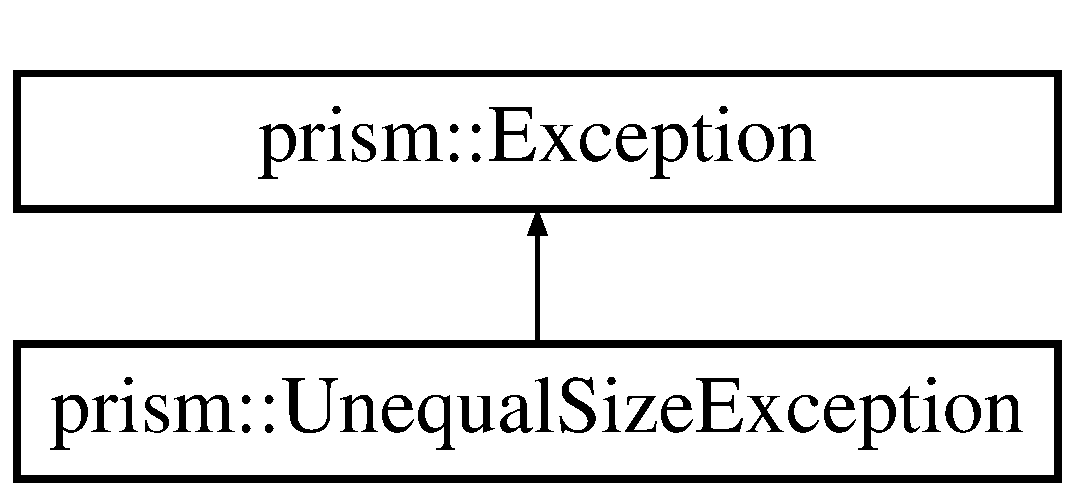
\includegraphics[height=2.000000cm]{classprism_1_1_unequal_size_exception}
\end{center}
\end{figure}
\subsection*{Public Member Functions}
\begin{DoxyCompactItemize}
\item 
\hyperlink{classprism_1_1_unequal_size_exception_a296effd83c180fe9c2eaa3b7f5acd233}{Unequal\+Size\+Exception} (const int sze1, const int sze2)
\end{DoxyCompactItemize}
\subsection*{Additional Inherited Members}


\subsection{Constructor \& Destructor Documentation}
\index{prism\+::\+Unequal\+Size\+Exception@{prism\+::\+Unequal\+Size\+Exception}!Unequal\+Size\+Exception@{Unequal\+Size\+Exception}}
\index{Unequal\+Size\+Exception@{Unequal\+Size\+Exception}!prism\+::\+Unequal\+Size\+Exception@{prism\+::\+Unequal\+Size\+Exception}}
\subsubsection[{\texorpdfstring{Unequal\+Size\+Exception(const int sze1, const int sze2)}{UnequalSizeException(const int sze1, const int sze2)}}]{\setlength{\rightskip}{0pt plus 5cm}prism\+::\+Unequal\+Size\+Exception\+::\+Unequal\+Size\+Exception (
\begin{DoxyParamCaption}
\item[{const int}]{sze1, }
\item[{const int}]{sze2}
\end{DoxyParamCaption}
)\hspace{0.3cm}{\ttfamily [inline]}}\hypertarget{classprism_1_1_unequal_size_exception_a296effd83c180fe9c2eaa3b7f5acd233}{}\label{classprism_1_1_unequal_size_exception_a296effd83c180fe9c2eaa3b7f5acd233}


The documentation for this class was generated from the following file\+:\begin{DoxyCompactItemize}
\item 
inc/prism/\hyperlink{_unequal_size_exception_8h}{Unequal\+Size\+Exception.\+h}\end{DoxyCompactItemize}

\hypertarget{classprism_1_1_vector}{}\section{prism\+:\+:Vector$<$ T $>$ Class Template Reference}
\label{classprism_1_1_vector}\index{prism\+::\+Vector$<$ T $>$@{prism\+::\+Vector$<$ T $>$}}


{\ttfamily \#include $<$Vector.\+h$>$}

\subsection*{Public Types}
\begin{DoxyCompactItemize}
\item 
typedef \hyperlink{classprism_1_1_random_access_iterator}{Random\+Access\+Iterator}$<$ T $>$ \hyperlink{classprism_1_1_vector_aa547779173a63f6f8c9b2887498d10eb}{iterator}
\item 
typedef \hyperlink{classprism_1_1_random_access_const_iterator}{Random\+Access\+Const\+Iterator}$<$ T $>$ \hyperlink{classprism_1_1_vector_acc6ed07e2d7ed5065feec92a83e46fa4}{const\+\_\+iterator}
\item 
typedef \hyperlink{classprism_1_1_forward_iterator_a4f7bff2c238f447c1537c74fe09f8935}{iterator\+::reference} \hyperlink{classprism_1_1_vector_a8ccf98342707efbed82918a44be97438}{reference}
\item 
typedef \hyperlink{classprism_1_1_forward_const_iterator_a839eeb121503b031260ad21ef844dd9a}{const\+\_\+iterator\+::reference} \hyperlink{classprism_1_1_vector_a75325487acaa0f63496c110e5a5632bb}{const\+\_\+reference}
\item 
typedef \hyperlink{classprism_1_1_forward_iterator_af50dd6e13f3cea3ee3b2332e48996502}{iterator\+::pointer} \hyperlink{classprism_1_1_vector_a9823d64f361cdff3fcc5043e8b4bd882}{pointer}
\item 
typedef \hyperlink{classprism_1_1_forward_const_iterator_a6e4e245d3ab99d6e9b237abe2c0c06d8}{const\+\_\+iterator\+::pointer} \hyperlink{classprism_1_1_vector_a0bf16322f83f0ad9103815a1cac16156}{const\+\_\+pointer}
\item 
typedef \hyperlink{classprism_1_1_forward_iterator_a7a28958d2cf2ea2613c6f0f011759781}{iterator\+::value\+\_\+type} \hyperlink{classprism_1_1_vector_a12f8585af6daa44e7732880b3f725ee3}{value\+\_\+type}
\item 
typedef \hyperlink{classprism_1_1_forward_iterator_a8c90486e85c02351c2e957ba3247ab10}{iterator\+::difference\+\_\+type} \hyperlink{classprism_1_1_vector_a5fe3b74bfb30d75aa74d4d896e6b7227}{difference\+\_\+type}
\item 
typedef int \hyperlink{classprism_1_1_vector_a14c909f500f13b8b7a276bb97ae746e8}{size\+\_\+type}
\end{DoxyCompactItemize}
\subsection*{Public Member Functions}
\begin{DoxyCompactItemize}
\item 
\hyperlink{classprism_1_1_vector_a0081b629c0ab4d85d6847a8cf382f1af}{Vector} ()
\item 
\hyperlink{classprism_1_1_vector_a61d37ac01e42fca59cdf320804a2a7ed}{Vector} (const int \hyperlink{classprism_1_1_vector_ac6ff3296683e76da61d48bcc15e4f175}{size}, const T \&value=T())
\item 
\hyperlink{classprism_1_1_vector_a6df8c0a101ff496b688f4937ec1f13e6}{Vector} (const \hyperlink{classprism_1_1_vector}{Vector}$<$ T $>$ \&\hyperlink{namespaceprism_ae776f4cd825f79e7af1cf6ee1d90a209}{copy})
\item 
\hyperlink{classprism_1_1_vector_a80f2790bb6011dd40739bff844fd3154}{$\sim$\+Vector} ()
\item 
void \hyperlink{classprism_1_1_vector_a690b3be3b217aab2842a5b9b7b0ab4dd}{append} (const T \&value)
\item 
T \& \hyperlink{classprism_1_1_vector_ad47f765360ae83602b645afe23a65541}{at} (const int index)
\item 
const T \& \hyperlink{classprism_1_1_vector_accf072a45a5be33b09d3210df16f52d5}{at} (const int index) const 
\item 
\hyperlink{classprism_1_1_vector_a8ccf98342707efbed82918a44be97438}{reference} \hyperlink{classprism_1_1_vector_a1e19cfd05c60f96f31fb4feba79fe4eb}{back} ()
\item 
\hyperlink{classprism_1_1_vector_a75325487acaa0f63496c110e5a5632bb}{const\+\_\+reference} \hyperlink{classprism_1_1_vector_abae5f68837ada40afa65d7ff492cc79f}{back} () const 
\item 
\hyperlink{classprism_1_1_vector_aa547779173a63f6f8c9b2887498d10eb}{iterator} \hyperlink{classprism_1_1_vector_a4e1871436d85d42653eddf9cf0dac271}{begin} ()
\item 
\hyperlink{classprism_1_1_vector_acc6ed07e2d7ed5065feec92a83e46fa4}{const\+\_\+iterator} \hyperlink{classprism_1_1_vector_a4cd1ca2ba159fd073127be98b37f6ba2}{begin} () const 
\item 
const int \hyperlink{classprism_1_1_vector_aa6bfbb4672a51177c6fafbd503e90a92}{capacity} () const 
\item 
\hyperlink{classprism_1_1_vector_acc6ed07e2d7ed5065feec92a83e46fa4}{const\+\_\+iterator} \hyperlink{classprism_1_1_vector_a3cb4a9878dfd0b58b8e0a5c01f5d37f5}{cbegin} () const 
\item 
\hyperlink{classprism_1_1_vector_acc6ed07e2d7ed5065feec92a83e46fa4}{const\+\_\+iterator} \hyperlink{classprism_1_1_vector_a3ac39de85562660281a0fd7601ef203b}{cend} () const 
\item 
void \hyperlink{classprism_1_1_vector_acb8a681b958856d257b145930014c6fa}{clear} ()
\item 
\hyperlink{classprism_1_1_vector_acc6ed07e2d7ed5065feec92a83e46fa4}{const\+\_\+iterator} \hyperlink{classprism_1_1_vector_a6d03b3bb9cc1292e1698674080ff3334}{const\+Begin} () const 
\item 
const T $\ast$ \hyperlink{classprism_1_1_vector_a6e6fee098958130862af58cafeb27d65}{const\+Data} () const 
\item 
\hyperlink{classprism_1_1_vector_acc6ed07e2d7ed5065feec92a83e46fa4}{const\+\_\+iterator} \hyperlink{classprism_1_1_vector_a99331f9557172b3e3e34fb36f23e5cc5}{const\+End} () const 
\item 
const bool \hyperlink{classprism_1_1_vector_a6b21bf92cde4f91cb8d14efb4e315ea0}{contains} (const T \&value) const 
\item 
const int \hyperlink{classprism_1_1_vector_ad40e1dc908502680797f37312dda7a4f}{count} (const T \&value) const 
\item 
T $\ast$ \hyperlink{classprism_1_1_vector_a0da05f1f73ce9b35f3837bb7fca4a81e}{data} ()
\item 
const T $\ast$ \hyperlink{classprism_1_1_vector_a148789766065acd9338e8e6d4dcbdd2d}{data} () const 
\item 
const bool \hyperlink{classprism_1_1_vector_ad710950cfeaaf977ef629e69fc39b5a7}{empty} () const 
\item 
\hyperlink{classprism_1_1_vector_aa547779173a63f6f8c9b2887498d10eb}{iterator} \hyperlink{classprism_1_1_vector_a329f8549c259232b232e8f361bc4bcb1}{end} ()
\item 
\hyperlink{classprism_1_1_vector_acc6ed07e2d7ed5065feec92a83e46fa4}{const\+\_\+iterator} \hyperlink{classprism_1_1_vector_a0a5a10cd6cd6790d2b3e2546af742fc9}{end} () const 
\item 
const bool \hyperlink{classprism_1_1_vector_ae214a9cce9ac8cc215893eee20fd0e44}{ends\+With} (const T \&value) const 
\item 
\hyperlink{classprism_1_1_vector_aa547779173a63f6f8c9b2887498d10eb}{iterator} \hyperlink{classprism_1_1_vector_a540d12132c9a971d469c9d53a954f322}{erase} (\hyperlink{classprism_1_1_vector_aa547779173a63f6f8c9b2887498d10eb}{iterator} pos)
\item 
\hyperlink{classprism_1_1_vector_aa547779173a63f6f8c9b2887498d10eb}{iterator} \hyperlink{classprism_1_1_vector_a170f8c53a09729cd04396604a982df59}{erase} (\hyperlink{classprism_1_1_vector_aa547779173a63f6f8c9b2887498d10eb}{iterator} from, \hyperlink{classprism_1_1_vector_aa547779173a63f6f8c9b2887498d10eb}{iterator} to)
\item 
void \hyperlink{classprism_1_1_vector_af9d17a636c708324bd373fb521da2941}{fill} (const T \&value)
\item 
T \& \hyperlink{classprism_1_1_vector_a1e2ec6951430f9850702ef7c95a13166}{first} ()
\item 
const T \& \hyperlink{classprism_1_1_vector_a5615ffd739ddca3ecadcc4357c4842c3}{first} () const 
\item 
\hyperlink{classprism_1_1_vector_a8ccf98342707efbed82918a44be97438}{reference} \hyperlink{classprism_1_1_vector_af37b66eb994e45fdaff93bc649a0561f}{front} ()
\item 
\hyperlink{classprism_1_1_vector_a75325487acaa0f63496c110e5a5632bb}{const\+\_\+reference} \hyperlink{classprism_1_1_vector_a3785411f25c191f68341fd8395d15440}{front} () const 
\item 
const int \hyperlink{classprism_1_1_vector_a0d0b833ffc1bc666624416e3b65181b4}{index\+Of} (const T \&value, const int from=0) const 
\item 
void \hyperlink{classprism_1_1_vector_aa9d6409134a4242f10ed6dbed1c5a91d}{insert} (const int index, const T \&value)
\item 
void \hyperlink{classprism_1_1_vector_a2712cf9aaa506332ae150e9e3f60abed}{insert} (const int index, const int \hyperlink{classprism_1_1_vector_ad40e1dc908502680797f37312dda7a4f}{count}, const T \&value)
\item 
\hyperlink{classprism_1_1_vector_aa547779173a63f6f8c9b2887498d10eb}{iterator} \hyperlink{classprism_1_1_vector_ac665dc2e7c506656fb4bbe3db303159c}{insert} (\hyperlink{classprism_1_1_vector_aa547779173a63f6f8c9b2887498d10eb}{iterator} insert\+Before, const T \&value)
\item 
\hyperlink{classprism_1_1_vector_aa547779173a63f6f8c9b2887498d10eb}{iterator} \hyperlink{classprism_1_1_vector_abbbb5974eb963ef66153271a4b6adf52}{insert} (\hyperlink{classprism_1_1_vector_aa547779173a63f6f8c9b2887498d10eb}{iterator} insert\+Before, const int \hyperlink{classprism_1_1_vector_ad40e1dc908502680797f37312dda7a4f}{count}, const T \&value)
\item 
const bool \hyperlink{classprism_1_1_vector_a23be1fddbb4bc27cabd6af5d1aa4ba91}{is\+Empty} () const 
\item 
T \& \hyperlink{classprism_1_1_vector_aa03291f774fc83f46972b07672fc616c}{last} ()
\item 
const T \& \hyperlink{classprism_1_1_vector_a8298d925eeb3a3be9e68d874112daf8c}{last} () const 
\item 
const int \hyperlink{classprism_1_1_vector_a33e965cfc15bd23e0748dfacaeb97428}{last\+Index\+Of} (const T \&value, const int from=-\/1) const 
\item 
\hyperlink{classprism_1_1_vector}{Vector}$<$ T $>$ \hyperlink{classprism_1_1_vector_ad15f2817fe441c22bbbdb1e1ecfe9aed}{mid} (const int start\+Index, const int \hyperlink{classprism_1_1_vector_ad40e1dc908502680797f37312dda7a4f}{count}=-\/1)
\item 
void \hyperlink{classprism_1_1_vector_a990628b9b119ddcec57715cd7541ea99}{pop\+\_\+back} ()
\item 
void \hyperlink{classprism_1_1_vector_abd9320b7ae720bb4c3500ebba3e42537}{pop\+\_\+front} ()
\item 
void \hyperlink{classprism_1_1_vector_a1438597636b56d6c9f522e719097190c}{prepend} (const T \&value)
\item 
void \hyperlink{classprism_1_1_vector_a4a920a4960f25c0aef5461eb46a2620e}{push\+\_\+back} (const T \&value)
\item 
void \hyperlink{classprism_1_1_vector_ad1f9542ba64a36ffbd10ede7cae95aef}{push\+\_\+front} (const T \&value)
\item 
void \hyperlink{classprism_1_1_vector_a5a1f891782e1bb2cba1bbe89a9b8afc7}{remove} (const int index)
\item 
void \hyperlink{classprism_1_1_vector_a2b9dcf29eefe01b99a83ec5c2189b487}{remove} (const int index, const int \hyperlink{classprism_1_1_vector_ad40e1dc908502680797f37312dda7a4f}{count})
\item 
void \hyperlink{classprism_1_1_vector_a9f44c797424ce88caf23a50486846b9d}{remove\+All} (const T \&value)
\item 
void \hyperlink{classprism_1_1_vector_a3a2287f445b6788a38a746b448f98b48}{remove\+First} ()
\item 
void \hyperlink{classprism_1_1_vector_a0d2d2724f9ba5a520159ddce1c9b4681}{remove\+Last} ()
\item 
void \hyperlink{classprism_1_1_vector_a6efd18c9c21f2a98f59ccea0ae2b694c}{replace} (const int index, const T \&value)
\item 
void \hyperlink{classprism_1_1_vector_a617fa4a86aca478131d33984c01118ae}{reserve} (const int new\+Capacity)
\item 
void \hyperlink{classprism_1_1_vector_a13675c55c77df670075a9f80057d1d2e}{resize} (const int new\+Size)
\item 
const int \hyperlink{classprism_1_1_vector_ac6ff3296683e76da61d48bcc15e4f175}{size} () const 
\item 
void \hyperlink{classprism_1_1_vector_ab2491ac6ff73d372ed8f080adef78208}{squeeze} ()
\item 
const bool \hyperlink{classprism_1_1_vector_a7562a7e62555ee5cc35b309799cbfb05}{starts\+With} (const T \&value) const 
\item 
\hyperlink{classprism_1_1_list}{List}$<$ T $>$ \hyperlink{classprism_1_1_vector_a129dfc6925b70bb736a4539bcb323de9}{to\+List} () const 
\item 
std\+::vector$<$ T $>$ \hyperlink{classprism_1_1_vector_ae84be49ceac4011b35dd81218324b7df}{to\+Std\+Vector} () const 
\item 
T \& \hyperlink{classprism_1_1_vector_a98144a18b30f486f276bd7420db4f012}{operator\mbox{[}$\,$\mbox{]}} (const int index)
\item 
const T \& \hyperlink{classprism_1_1_vector_aec9d5e00c9127674735e321217fe3728}{operator\mbox{[}$\,$\mbox{]}} (const int index) const 
\item 
\hyperlink{classprism_1_1_vector}{Vector}$<$ T $>$ \& \hyperlink{classprism_1_1_vector_a687da3b48a2087e6e07fd5219389adb3}{operator$<$$<$} (const T \&value)
\item 
\hyperlink{classprism_1_1_vector}{Vector}$<$ T $>$ \& \hyperlink{classprism_1_1_vector_a63456dd4a36f843522f6312f0c3032e7}{operator$<$$<$} (const \hyperlink{classprism_1_1_vector}{Vector}$<$ T $>$ \&rhs)
\item 
\hyperlink{classprism_1_1_vector}{Vector}$<$ T $>$ \& \hyperlink{classprism_1_1_vector_a8e248700c87a2176c675c91d4f6a4390}{operator=} (const \hyperlink{classprism_1_1_vector}{Vector}$<$ T $>$ \&rhs)
\item 
const bool \hyperlink{classprism_1_1_vector_aedbb9a32bb25fe4bc5907fa498fe6534}{operator==} (const \hyperlink{classprism_1_1_vector}{Vector}$<$ T $>$ \&rhs) const 
\item 
const bool \hyperlink{classprism_1_1_vector_a7f3b55afc7268eba0f06a16f54b66b0c}{operator!=} (const \hyperlink{classprism_1_1_vector}{Vector}$<$ T $>$ \&rhs) const 
\item 
\hyperlink{classprism_1_1_vector}{Vector}$<$ T $>$ \hyperlink{classprism_1_1_vector_a9275846b38b6ce971d7d7114bca5acc2}{operator+} (const \hyperlink{classprism_1_1_vector}{Vector}$<$ T $>$ \&rhs) const 
\item 
\hyperlink{classprism_1_1_vector}{Vector}$<$ T $>$ \& \hyperlink{classprism_1_1_vector_a094f14b6f6f219dda41b0b7879d9b6b5}{operator+=} (const \hyperlink{classprism_1_1_vector}{Vector}$<$ T $>$ \&rhs)
\end{DoxyCompactItemize}
\subsection*{Static Public Member Functions}
\begin{DoxyCompactItemize}
\item 
static \hyperlink{classprism_1_1_vector}{Vector}$<$ T $>$ \hyperlink{classprism_1_1_vector_a66de66a61b4577aa20f6a6f5e4b8e99d}{from\+List} (const \hyperlink{classprism_1_1_list}{List}$<$ T $>$ \&list)
\item 
static \hyperlink{classprism_1_1_vector}{Vector}$<$ T $>$ \hyperlink{classprism_1_1_vector_ac947685add7d54b025a471b59445fc6a}{from\+Std\+Vector} (const std\+::vector$<$ T $>$ \&std\+Vec)
\end{DoxyCompactItemize}
\subsection*{Friends}
\begin{DoxyCompactItemize}
\item 
std\+::ostream \& \hyperlink{classprism_1_1_vector_adea1a7e2e26629669d11a49d8899a1ec}{operator$<$$<$} (std\+::ostream \&out, const \hyperlink{classprism_1_1_vector}{Vector}$<$ T $>$ \&v)
\end{DoxyCompactItemize}


\subsection{Member Typedef Documentation}
\index{prism\+::\+Vector@{prism\+::\+Vector}!const\+\_\+iterator@{const\+\_\+iterator}}
\index{const\+\_\+iterator@{const\+\_\+iterator}!prism\+::\+Vector@{prism\+::\+Vector}}
\subsubsection[{\texorpdfstring{const\+\_\+iterator}{const_iterator}}]{\setlength{\rightskip}{0pt plus 5cm}template$<$class T$>$ typedef {\bf Random\+Access\+Const\+Iterator}$<$T$>$ {\bf prism\+::\+Vector}$<$ T $>$\+::{\bf const\+\_\+iterator}}\hypertarget{classprism_1_1_vector_acc6ed07e2d7ed5065feec92a83e46fa4}{}\label{classprism_1_1_vector_acc6ed07e2d7ed5065feec92a83e46fa4}
\index{prism\+::\+Vector@{prism\+::\+Vector}!const\+\_\+pointer@{const\+\_\+pointer}}
\index{const\+\_\+pointer@{const\+\_\+pointer}!prism\+::\+Vector@{prism\+::\+Vector}}
\subsubsection[{\texorpdfstring{const\+\_\+pointer}{const_pointer}}]{\setlength{\rightskip}{0pt plus 5cm}template$<$class T$>$ typedef {\bf const\+\_\+iterator\+::pointer} {\bf prism\+::\+Vector}$<$ T $>$\+::{\bf const\+\_\+pointer}}\hypertarget{classprism_1_1_vector_a0bf16322f83f0ad9103815a1cac16156}{}\label{classprism_1_1_vector_a0bf16322f83f0ad9103815a1cac16156}
\index{prism\+::\+Vector@{prism\+::\+Vector}!const\+\_\+reference@{const\+\_\+reference}}
\index{const\+\_\+reference@{const\+\_\+reference}!prism\+::\+Vector@{prism\+::\+Vector}}
\subsubsection[{\texorpdfstring{const\+\_\+reference}{const_reference}}]{\setlength{\rightskip}{0pt plus 5cm}template$<$class T$>$ typedef {\bf const\+\_\+iterator\+::reference} {\bf prism\+::\+Vector}$<$ T $>$\+::{\bf const\+\_\+reference}}\hypertarget{classprism_1_1_vector_a75325487acaa0f63496c110e5a5632bb}{}\label{classprism_1_1_vector_a75325487acaa0f63496c110e5a5632bb}
\index{prism\+::\+Vector@{prism\+::\+Vector}!difference\+\_\+type@{difference\+\_\+type}}
\index{difference\+\_\+type@{difference\+\_\+type}!prism\+::\+Vector@{prism\+::\+Vector}}
\subsubsection[{\texorpdfstring{difference\+\_\+type}{difference_type}}]{\setlength{\rightskip}{0pt plus 5cm}template$<$class T$>$ typedef {\bf iterator\+::difference\+\_\+type} {\bf prism\+::\+Vector}$<$ T $>$\+::{\bf difference\+\_\+type}}\hypertarget{classprism_1_1_vector_a5fe3b74bfb30d75aa74d4d896e6b7227}{}\label{classprism_1_1_vector_a5fe3b74bfb30d75aa74d4d896e6b7227}
\index{prism\+::\+Vector@{prism\+::\+Vector}!iterator@{iterator}}
\index{iterator@{iterator}!prism\+::\+Vector@{prism\+::\+Vector}}
\subsubsection[{\texorpdfstring{iterator}{iterator}}]{\setlength{\rightskip}{0pt plus 5cm}template$<$class T$>$ typedef {\bf Random\+Access\+Iterator}$<$T$>$ {\bf prism\+::\+Vector}$<$ T $>$\+::{\bf iterator}}\hypertarget{classprism_1_1_vector_aa547779173a63f6f8c9b2887498d10eb}{}\label{classprism_1_1_vector_aa547779173a63f6f8c9b2887498d10eb}
\index{prism\+::\+Vector@{prism\+::\+Vector}!pointer@{pointer}}
\index{pointer@{pointer}!prism\+::\+Vector@{prism\+::\+Vector}}
\subsubsection[{\texorpdfstring{pointer}{pointer}}]{\setlength{\rightskip}{0pt plus 5cm}template$<$class T$>$ typedef {\bf iterator\+::pointer} {\bf prism\+::\+Vector}$<$ T $>$\+::{\bf pointer}}\hypertarget{classprism_1_1_vector_a9823d64f361cdff3fcc5043e8b4bd882}{}\label{classprism_1_1_vector_a9823d64f361cdff3fcc5043e8b4bd882}
\index{prism\+::\+Vector@{prism\+::\+Vector}!reference@{reference}}
\index{reference@{reference}!prism\+::\+Vector@{prism\+::\+Vector}}
\subsubsection[{\texorpdfstring{reference}{reference}}]{\setlength{\rightskip}{0pt plus 5cm}template$<$class T$>$ typedef {\bf iterator\+::reference} {\bf prism\+::\+Vector}$<$ T $>$\+::{\bf reference}}\hypertarget{classprism_1_1_vector_a8ccf98342707efbed82918a44be97438}{}\label{classprism_1_1_vector_a8ccf98342707efbed82918a44be97438}
\index{prism\+::\+Vector@{prism\+::\+Vector}!size\+\_\+type@{size\+\_\+type}}
\index{size\+\_\+type@{size\+\_\+type}!prism\+::\+Vector@{prism\+::\+Vector}}
\subsubsection[{\texorpdfstring{size\+\_\+type}{size_type}}]{\setlength{\rightskip}{0pt plus 5cm}template$<$class T$>$ typedef int {\bf prism\+::\+Vector}$<$ T $>$\+::{\bf size\+\_\+type}}\hypertarget{classprism_1_1_vector_a14c909f500f13b8b7a276bb97ae746e8}{}\label{classprism_1_1_vector_a14c909f500f13b8b7a276bb97ae746e8}
\index{prism\+::\+Vector@{prism\+::\+Vector}!value\+\_\+type@{value\+\_\+type}}
\index{value\+\_\+type@{value\+\_\+type}!prism\+::\+Vector@{prism\+::\+Vector}}
\subsubsection[{\texorpdfstring{value\+\_\+type}{value_type}}]{\setlength{\rightskip}{0pt plus 5cm}template$<$class T$>$ typedef {\bf iterator\+::value\+\_\+type} {\bf prism\+::\+Vector}$<$ T $>$\+::{\bf value\+\_\+type}}\hypertarget{classprism_1_1_vector_a12f8585af6daa44e7732880b3f725ee3}{}\label{classprism_1_1_vector_a12f8585af6daa44e7732880b3f725ee3}


\subsection{Constructor \& Destructor Documentation}
\index{prism\+::\+Vector@{prism\+::\+Vector}!Vector@{Vector}}
\index{Vector@{Vector}!prism\+::\+Vector@{prism\+::\+Vector}}
\subsubsection[{\texorpdfstring{Vector()}{Vector()}}]{\setlength{\rightskip}{0pt plus 5cm}template$<$class T $>$ {\bf prism\+::\+Vector}$<$ T $>$\+::{\bf Vector} (
\begin{DoxyParamCaption}
{}
\end{DoxyParamCaption}
)}\hypertarget{classprism_1_1_vector_a0081b629c0ab4d85d6847a8cf382f1af}{}\label{classprism_1_1_vector_a0081b629c0ab4d85d6847a8cf382f1af}
Creates an empty vector. \index{prism\+::\+Vector@{prism\+::\+Vector}!Vector@{Vector}}
\index{Vector@{Vector}!prism\+::\+Vector@{prism\+::\+Vector}}
\subsubsection[{\texorpdfstring{Vector(const int size, const T \&value=\+T())}{Vector(const int size, const T &value=T())}}]{\setlength{\rightskip}{0pt plus 5cm}template$<$class T $>$ {\bf prism\+::\+Vector}$<$ T $>$\+::{\bf Vector} (
\begin{DoxyParamCaption}
\item[{const int}]{size, }
\item[{const T \&}]{value = {\ttfamily T()}}
\end{DoxyParamCaption}
)}\hypertarget{classprism_1_1_vector_a61d37ac01e42fca59cdf320804a2a7ed}{}\label{classprism_1_1_vector_a61d37ac01e42fca59cdf320804a2a7ed}
Creates a vector containing {\itshape size} elements setting each value to its default constructed value i.\+e. T() if a value is not provided. If a value is provided then each element is set to {\itshape value}. \index{prism\+::\+Vector@{prism\+::\+Vector}!Vector@{Vector}}
\index{Vector@{Vector}!prism\+::\+Vector@{prism\+::\+Vector}}
\subsubsection[{\texorpdfstring{Vector(const Vector$<$ T $>$ \&copy)}{Vector(const Vector< T > &copy)}}]{\setlength{\rightskip}{0pt plus 5cm}template$<$class T $>$ {\bf prism\+::\+Vector}$<$ T $>$\+::{\bf Vector} (
\begin{DoxyParamCaption}
\item[{const {\bf Vector}$<$ T $>$ \&}]{copy}
\end{DoxyParamCaption}
)}\hypertarget{classprism_1_1_vector_a6df8c0a101ff496b688f4937ec1f13e6}{}\label{classprism_1_1_vector_a6df8c0a101ff496b688f4937ec1f13e6}
Copy-\/constructs a new vector that will contain all of the elements from {\itshape copy}. \index{prism\+::\+Vector@{prism\+::\+Vector}!````~Vector@{$\sim$\+Vector}}
\index{````~Vector@{$\sim$\+Vector}!prism\+::\+Vector@{prism\+::\+Vector}}
\subsubsection[{\texorpdfstring{$\sim$\+Vector()}{~Vector()}}]{\setlength{\rightskip}{0pt plus 5cm}template$<$class T $>$ {\bf prism\+::\+Vector}$<$ T $>$\+::$\sim${\bf Vector} (
\begin{DoxyParamCaption}
{}
\end{DoxyParamCaption}
)}\hypertarget{classprism_1_1_vector_a80f2790bb6011dd40739bff844fd3154}{}\label{classprism_1_1_vector_a80f2790bb6011dd40739bff844fd3154}
Destroys this vector. 

\subsection{Member Function Documentation}
\index{prism\+::\+Vector@{prism\+::\+Vector}!append@{append}}
\index{append@{append}!prism\+::\+Vector@{prism\+::\+Vector}}
\subsubsection[{\texorpdfstring{append(const T \&value)}{append(const T &value)}}]{\setlength{\rightskip}{0pt plus 5cm}template$<$class T $>$ void {\bf prism\+::\+Vector}$<$ T $>$\+::append (
\begin{DoxyParamCaption}
\item[{const T \&}]{value}
\end{DoxyParamCaption}
)}\hypertarget{classprism_1_1_vector_a690b3be3b217aab2842a5b9b7b0ab4dd}{}\label{classprism_1_1_vector_a690b3be3b217aab2842a5b9b7b0ab4dd}
Appends {\itshape value} to the end of the vector. \index{prism\+::\+Vector@{prism\+::\+Vector}!at@{at}}
\index{at@{at}!prism\+::\+Vector@{prism\+::\+Vector}}
\subsubsection[{\texorpdfstring{at(const int index)}{at(const int index)}}]{\setlength{\rightskip}{0pt plus 5cm}template$<$class T $>$ T \& {\bf prism\+::\+Vector}$<$ T $>$\+::at (
\begin{DoxyParamCaption}
\item[{const int}]{index}
\end{DoxyParamCaption}
)}\hypertarget{classprism_1_1_vector_ad47f765360ae83602b645afe23a65541}{}\label{classprism_1_1_vector_ad47f765360ae83602b645afe23a65541}
Returns a reference to the element at {\itshape index}. {\itshape index} must be 0$<$=index$<$\hyperlink{classprism_1_1_vector_ac6ff3296683e76da61d48bcc15e4f175}{size()}. \index{prism\+::\+Vector@{prism\+::\+Vector}!at@{at}}
\index{at@{at}!prism\+::\+Vector@{prism\+::\+Vector}}
\subsubsection[{\texorpdfstring{at(const int index) const }{at(const int index) const }}]{\setlength{\rightskip}{0pt plus 5cm}template$<$class T $>$ const T \& {\bf prism\+::\+Vector}$<$ T $>$\+::at (
\begin{DoxyParamCaption}
\item[{const int}]{index}
\end{DoxyParamCaption}
) const}\hypertarget{classprism_1_1_vector_accf072a45a5be33b09d3210df16f52d5}{}\label{classprism_1_1_vector_accf072a45a5be33b09d3210df16f52d5}
Returns a const reference to the element at {\itshape index}. {\itshape index} must be 0$<$=index$<$\hyperlink{classprism_1_1_vector_ac6ff3296683e76da61d48bcc15e4f175}{size()}. \index{prism\+::\+Vector@{prism\+::\+Vector}!back@{back}}
\index{back@{back}!prism\+::\+Vector@{prism\+::\+Vector}}
\subsubsection[{\texorpdfstring{back()}{back()}}]{\setlength{\rightskip}{0pt plus 5cm}template$<$class T $>$ {\bf Vector}$<$ T $>$\+::{\bf reference} {\bf prism\+::\+Vector}$<$ T $>$\+::back (
\begin{DoxyParamCaption}
{}
\end{DoxyParamCaption}
)}\hypertarget{classprism_1_1_vector_a1e19cfd05c60f96f31fb4feba79fe4eb}{}\label{classprism_1_1_vector_a1e19cfd05c60f96f31fb4feba79fe4eb}
Returns a reference to the last element in the vector. \index{prism\+::\+Vector@{prism\+::\+Vector}!back@{back}}
\index{back@{back}!prism\+::\+Vector@{prism\+::\+Vector}}
\subsubsection[{\texorpdfstring{back() const }{back() const }}]{\setlength{\rightskip}{0pt plus 5cm}template$<$class T $>$ {\bf Vector}$<$ T $>$\+::{\bf const\+\_\+reference} {\bf prism\+::\+Vector}$<$ T $>$\+::back (
\begin{DoxyParamCaption}
{}
\end{DoxyParamCaption}
) const}\hypertarget{classprism_1_1_vector_abae5f68837ada40afa65d7ff492cc79f}{}\label{classprism_1_1_vector_abae5f68837ada40afa65d7ff492cc79f}
Returns a const reference to the last element in the vector. \index{prism\+::\+Vector@{prism\+::\+Vector}!begin@{begin}}
\index{begin@{begin}!prism\+::\+Vector@{prism\+::\+Vector}}
\subsubsection[{\texorpdfstring{begin()}{begin()}}]{\setlength{\rightskip}{0pt plus 5cm}template$<$class T $>$ {\bf Vector}$<$ T $>$\+::{\bf iterator} {\bf prism\+::\+Vector}$<$ T $>$\+::begin (
\begin{DoxyParamCaption}
{}
\end{DoxyParamCaption}
)}\hypertarget{classprism_1_1_vector_a4e1871436d85d42653eddf9cf0dac271}{}\label{classprism_1_1_vector_a4e1871436d85d42653eddf9cf0dac271}
Returns an iterator that points to the first element in the vector. \index{prism\+::\+Vector@{prism\+::\+Vector}!begin@{begin}}
\index{begin@{begin}!prism\+::\+Vector@{prism\+::\+Vector}}
\subsubsection[{\texorpdfstring{begin() const }{begin() const }}]{\setlength{\rightskip}{0pt plus 5cm}template$<$class T $>$ {\bf Vector}$<$ T $>$\+::{\bf const\+\_\+iterator} {\bf prism\+::\+Vector}$<$ T $>$\+::begin (
\begin{DoxyParamCaption}
{}
\end{DoxyParamCaption}
) const}\hypertarget{classprism_1_1_vector_a4cd1ca2ba159fd073127be98b37f6ba2}{}\label{classprism_1_1_vector_a4cd1ca2ba159fd073127be98b37f6ba2}
Returns a const iterator that points to the first element in the vector. \index{prism\+::\+Vector@{prism\+::\+Vector}!capacity@{capacity}}
\index{capacity@{capacity}!prism\+::\+Vector@{prism\+::\+Vector}}
\subsubsection[{\texorpdfstring{capacity() const }{capacity() const }}]{\setlength{\rightskip}{0pt plus 5cm}template$<$class T $>$ const int {\bf prism\+::\+Vector}$<$ T $>$\+::capacity (
\begin{DoxyParamCaption}
{}
\end{DoxyParamCaption}
) const}\hypertarget{classprism_1_1_vector_aa6bfbb4672a51177c6fafbd503e90a92}{}\label{classprism_1_1_vector_aa6bfbb4672a51177c6fafbd503e90a92}
Returns the capacity of the vector. \index{prism\+::\+Vector@{prism\+::\+Vector}!cbegin@{cbegin}}
\index{cbegin@{cbegin}!prism\+::\+Vector@{prism\+::\+Vector}}
\subsubsection[{\texorpdfstring{cbegin() const }{cbegin() const }}]{\setlength{\rightskip}{0pt plus 5cm}template$<$class T $>$ {\bf Vector}$<$ T $>$\+::{\bf const\+\_\+iterator} {\bf prism\+::\+Vector}$<$ T $>$\+::cbegin (
\begin{DoxyParamCaption}
{}
\end{DoxyParamCaption}
) const}\hypertarget{classprism_1_1_vector_a3cb4a9878dfd0b58b8e0a5c01f5d37f5}{}\label{classprism_1_1_vector_a3cb4a9878dfd0b58b8e0a5c01f5d37f5}
Returns a const iterator that points to the first element in the vector. \index{prism\+::\+Vector@{prism\+::\+Vector}!cend@{cend}}
\index{cend@{cend}!prism\+::\+Vector@{prism\+::\+Vector}}
\subsubsection[{\texorpdfstring{cend() const }{cend() const }}]{\setlength{\rightskip}{0pt plus 5cm}template$<$class T $>$ {\bf Vector}$<$ T $>$\+::{\bf const\+\_\+iterator} {\bf prism\+::\+Vector}$<$ T $>$\+::cend (
\begin{DoxyParamCaption}
{}
\end{DoxyParamCaption}
) const}\hypertarget{classprism_1_1_vector_a3ac39de85562660281a0fd7601ef203b}{}\label{classprism_1_1_vector_a3ac39de85562660281a0fd7601ef203b}
Returns a const iterator that points to the imaginary element one after the last value in the vector. \index{prism\+::\+Vector@{prism\+::\+Vector}!clear@{clear}}
\index{clear@{clear}!prism\+::\+Vector@{prism\+::\+Vector}}
\subsubsection[{\texorpdfstring{clear()}{clear()}}]{\setlength{\rightskip}{0pt plus 5cm}template$<$class T $>$ void {\bf prism\+::\+Vector}$<$ T $>$\+::clear (
\begin{DoxyParamCaption}
{}
\end{DoxyParamCaption}
)}\hypertarget{classprism_1_1_vector_acb8a681b958856d257b145930014c6fa}{}\label{classprism_1_1_vector_acb8a681b958856d257b145930014c6fa}
Removes all elements from the vector leaving a size of 0. The capacity however remains unchanged although can shrunk using \hyperlink{classprism_1_1_vector_ab2491ac6ff73d372ed8f080adef78208}{squeeze()} if required. \index{prism\+::\+Vector@{prism\+::\+Vector}!const\+Begin@{const\+Begin}}
\index{const\+Begin@{const\+Begin}!prism\+::\+Vector@{prism\+::\+Vector}}
\subsubsection[{\texorpdfstring{const\+Begin() const }{constBegin() const }}]{\setlength{\rightskip}{0pt plus 5cm}template$<$class T $>$ {\bf Vector}$<$ T $>$\+::{\bf const\+\_\+iterator} {\bf prism\+::\+Vector}$<$ T $>$\+::const\+Begin (
\begin{DoxyParamCaption}
{}
\end{DoxyParamCaption}
) const}\hypertarget{classprism_1_1_vector_a6d03b3bb9cc1292e1698674080ff3334}{}\label{classprism_1_1_vector_a6d03b3bb9cc1292e1698674080ff3334}
Returns a const iterator that points to the first element in the vector. \index{prism\+::\+Vector@{prism\+::\+Vector}!const\+Data@{const\+Data}}
\index{const\+Data@{const\+Data}!prism\+::\+Vector@{prism\+::\+Vector}}
\subsubsection[{\texorpdfstring{const\+Data() const }{constData() const }}]{\setlength{\rightskip}{0pt plus 5cm}template$<$class T $>$ const T $\ast$ {\bf prism\+::\+Vector}$<$ T $>$\+::const\+Data (
\begin{DoxyParamCaption}
{}
\end{DoxyParamCaption}
) const}\hypertarget{classprism_1_1_vector_a6e6fee098958130862af58cafeb27d65}{}\label{classprism_1_1_vector_a6e6fee098958130862af58cafeb27d65}
Returns a const pointer to the underlying array data. \index{prism\+::\+Vector@{prism\+::\+Vector}!const\+End@{const\+End}}
\index{const\+End@{const\+End}!prism\+::\+Vector@{prism\+::\+Vector}}
\subsubsection[{\texorpdfstring{const\+End() const }{constEnd() const }}]{\setlength{\rightskip}{0pt plus 5cm}template$<$class T $>$ {\bf Vector}$<$ T $>$\+::{\bf const\+\_\+iterator} {\bf prism\+::\+Vector}$<$ T $>$\+::const\+End (
\begin{DoxyParamCaption}
{}
\end{DoxyParamCaption}
) const}\hypertarget{classprism_1_1_vector_a99331f9557172b3e3e34fb36f23e5cc5}{}\label{classprism_1_1_vector_a99331f9557172b3e3e34fb36f23e5cc5}
Returns a const iterator that points to the imaginary element one after the last value in the vector. \index{prism\+::\+Vector@{prism\+::\+Vector}!contains@{contains}}
\index{contains@{contains}!prism\+::\+Vector@{prism\+::\+Vector}}
\subsubsection[{\texorpdfstring{contains(const T \&value) const }{contains(const T &value) const }}]{\setlength{\rightskip}{0pt plus 5cm}template$<$class T $>$ const bool {\bf prism\+::\+Vector}$<$ T $>$\+::contains (
\begin{DoxyParamCaption}
\item[{const T \&}]{value}
\end{DoxyParamCaption}
) const}\hypertarget{classprism_1_1_vector_a6b21bf92cde4f91cb8d14efb4e315ea0}{}\label{classprism_1_1_vector_a6b21bf92cde4f91cb8d14efb4e315ea0}
Returns true if the vector contains one or more occurrences of {\itshape value} and false otherwise. The vector\textquotesingle{}s value type must support \hyperlink{classprism_1_1_vector_aedbb9a32bb25fe4bc5907fa498fe6534}{operator==()}. \index{prism\+::\+Vector@{prism\+::\+Vector}!count@{count}}
\index{count@{count}!prism\+::\+Vector@{prism\+::\+Vector}}
\subsubsection[{\texorpdfstring{count(const T \&value) const }{count(const T &value) const }}]{\setlength{\rightskip}{0pt plus 5cm}template$<$class T $>$ const int {\bf prism\+::\+Vector}$<$ T $>$\+::count (
\begin{DoxyParamCaption}
\item[{const T \&}]{value}
\end{DoxyParamCaption}
) const}\hypertarget{classprism_1_1_vector_ad40e1dc908502680797f37312dda7a4f}{}\label{classprism_1_1_vector_ad40e1dc908502680797f37312dda7a4f}
Counts and returns the number of occurrences of /em value in the vector. The vector\textquotesingle{}s value type must support \hyperlink{classprism_1_1_vector_aedbb9a32bb25fe4bc5907fa498fe6534}{operator==()}. \index{prism\+::\+Vector@{prism\+::\+Vector}!data@{data}}
\index{data@{data}!prism\+::\+Vector@{prism\+::\+Vector}}
\subsubsection[{\texorpdfstring{data()}{data()}}]{\setlength{\rightskip}{0pt plus 5cm}template$<$class T $>$ T $\ast$ {\bf prism\+::\+Vector}$<$ T $>$\+::data (
\begin{DoxyParamCaption}
{}
\end{DoxyParamCaption}
)}\hypertarget{classprism_1_1_vector_a0da05f1f73ce9b35f3837bb7fca4a81e}{}\label{classprism_1_1_vector_a0da05f1f73ce9b35f3837bb7fca4a81e}
Returns a pointer to the underlying array data. \index{prism\+::\+Vector@{prism\+::\+Vector}!data@{data}}
\index{data@{data}!prism\+::\+Vector@{prism\+::\+Vector}}
\subsubsection[{\texorpdfstring{data() const }{data() const }}]{\setlength{\rightskip}{0pt plus 5cm}template$<$class T $>$ const T $\ast$ {\bf prism\+::\+Vector}$<$ T $>$\+::data (
\begin{DoxyParamCaption}
{}
\end{DoxyParamCaption}
) const}\hypertarget{classprism_1_1_vector_a148789766065acd9338e8e6d4dcbdd2d}{}\label{classprism_1_1_vector_a148789766065acd9338e8e6d4dcbdd2d}
Returns a const pointer to the underlying array data. \index{prism\+::\+Vector@{prism\+::\+Vector}!empty@{empty}}
\index{empty@{empty}!prism\+::\+Vector@{prism\+::\+Vector}}
\subsubsection[{\texorpdfstring{empty() const }{empty() const }}]{\setlength{\rightskip}{0pt plus 5cm}template$<$class T $>$ const bool {\bf prism\+::\+Vector}$<$ T $>$\+::empty (
\begin{DoxyParamCaption}
{}
\end{DoxyParamCaption}
) const}\hypertarget{classprism_1_1_vector_ad710950cfeaaf977ef629e69fc39b5a7}{}\label{classprism_1_1_vector_ad710950cfeaaf977ef629e69fc39b5a7}
Returns true if this vector contains no elements i.\+e. size of 0 and false otherwise. Equivalent to \hyperlink{classprism_1_1_vector_a23be1fddbb4bc27cabd6af5d1aa4ba91}{is\+Empty()}. \index{prism\+::\+Vector@{prism\+::\+Vector}!end@{end}}
\index{end@{end}!prism\+::\+Vector@{prism\+::\+Vector}}
\subsubsection[{\texorpdfstring{end()}{end()}}]{\setlength{\rightskip}{0pt plus 5cm}template$<$class T $>$ {\bf Vector}$<$ T $>$\+::{\bf iterator} {\bf prism\+::\+Vector}$<$ T $>$\+::end (
\begin{DoxyParamCaption}
{}
\end{DoxyParamCaption}
)}\hypertarget{classprism_1_1_vector_a329f8549c259232b232e8f361bc4bcb1}{}\label{classprism_1_1_vector_a329f8549c259232b232e8f361bc4bcb1}
Returns an iterator to the imaginary element one position after the last value in the vector. \index{prism\+::\+Vector@{prism\+::\+Vector}!end@{end}}
\index{end@{end}!prism\+::\+Vector@{prism\+::\+Vector}}
\subsubsection[{\texorpdfstring{end() const }{end() const }}]{\setlength{\rightskip}{0pt plus 5cm}template$<$class T $>$ {\bf Vector}$<$ T $>$\+::{\bf const\+\_\+iterator} {\bf prism\+::\+Vector}$<$ T $>$\+::end (
\begin{DoxyParamCaption}
{}
\end{DoxyParamCaption}
) const}\hypertarget{classprism_1_1_vector_a0a5a10cd6cd6790d2b3e2546af742fc9}{}\label{classprism_1_1_vector_a0a5a10cd6cd6790d2b3e2546af742fc9}
Returns a const iterator to the imaginary element one position after the last value in the vector. \index{prism\+::\+Vector@{prism\+::\+Vector}!ends\+With@{ends\+With}}
\index{ends\+With@{ends\+With}!prism\+::\+Vector@{prism\+::\+Vector}}
\subsubsection[{\texorpdfstring{ends\+With(const T \&value) const }{endsWith(const T &value) const }}]{\setlength{\rightskip}{0pt plus 5cm}template$<$class T $>$ const bool {\bf prism\+::\+Vector}$<$ T $>$\+::ends\+With (
\begin{DoxyParamCaption}
\item[{const T \&}]{value}
\end{DoxyParamCaption}
) const}\hypertarget{classprism_1_1_vector_ae214a9cce9ac8cc215893eee20fd0e44}{}\label{classprism_1_1_vector_ae214a9cce9ac8cc215893eee20fd0e44}
Returns true if the vector is not empty and its last element is equal to {\itshape value} and false otherwise. The vector\textquotesingle{}s value type must support \hyperlink{classprism_1_1_vector_aedbb9a32bb25fe4bc5907fa498fe6534}{operator==()}. \index{prism\+::\+Vector@{prism\+::\+Vector}!erase@{erase}}
\index{erase@{erase}!prism\+::\+Vector@{prism\+::\+Vector}}
\subsubsection[{\texorpdfstring{erase(iterator pos)}{erase(iterator pos)}}]{\setlength{\rightskip}{0pt plus 5cm}template$<$class T $>$ {\bf Vector}$<$ T $>$\+::{\bf iterator} {\bf prism\+::\+Vector}$<$ T $>$\+::erase (
\begin{DoxyParamCaption}
\item[{{\bf iterator}}]{pos}
\end{DoxyParamCaption}
)}\hypertarget{classprism_1_1_vector_a540d12132c9a971d469c9d53a954f322}{}\label{classprism_1_1_vector_a540d12132c9a971d469c9d53a954f322}
Erases the element pointed to by {\itshape pos}. Returns an iterator to the next position (which could be \hyperlink{classprism_1_1_vector_a329f8549c259232b232e8f361bc4bcb1}{end()}). \index{prism\+::\+Vector@{prism\+::\+Vector}!erase@{erase}}
\index{erase@{erase}!prism\+::\+Vector@{prism\+::\+Vector}}
\subsubsection[{\texorpdfstring{erase(iterator from, iterator to)}{erase(iterator from, iterator to)}}]{\setlength{\rightskip}{0pt plus 5cm}template$<$class T $>$ {\bf Vector}$<$ T $>$\+::{\bf iterator} {\bf prism\+::\+Vector}$<$ T $>$\+::erase (
\begin{DoxyParamCaption}
\item[{{\bf iterator}}]{from, }
\item[{{\bf iterator}}]{to}
\end{DoxyParamCaption}
)}\hypertarget{classprism_1_1_vector_a170f8c53a09729cd04396604a982df59}{}\label{classprism_1_1_vector_a170f8c53a09729cd04396604a982df59}
Erases the elements pointed to by the iterator range of {\itshape from} and {\itshape to}. Every element from {\itshape from} up to (but not including {\itshape to}) is erased. Returns an iterator to the first element after the erased elements (could be equal to \hyperlink{classprism_1_1_vector_a329f8549c259232b232e8f361bc4bcb1}{end()}). \index{prism\+::\+Vector@{prism\+::\+Vector}!fill@{fill}}
\index{fill@{fill}!prism\+::\+Vector@{prism\+::\+Vector}}
\subsubsection[{\texorpdfstring{fill(const T \&value)}{fill(const T &value)}}]{\setlength{\rightskip}{0pt plus 5cm}template$<$class T $>$ void {\bf prism\+::\+Vector}$<$ T $>$\+::fill (
\begin{DoxyParamCaption}
\item[{const T \&}]{value}
\end{DoxyParamCaption}
)}\hypertarget{classprism_1_1_vector_af9d17a636c708324bd373fb521da2941}{}\label{classprism_1_1_vector_af9d17a636c708324bd373fb521da2941}
Assigns {\itshape value} to every element in the vector. \index{prism\+::\+Vector@{prism\+::\+Vector}!first@{first}}
\index{first@{first}!prism\+::\+Vector@{prism\+::\+Vector}}
\subsubsection[{\texorpdfstring{first()}{first()}}]{\setlength{\rightskip}{0pt plus 5cm}template$<$class T $>$ T \& {\bf prism\+::\+Vector}$<$ T $>$\+::first (
\begin{DoxyParamCaption}
{}
\end{DoxyParamCaption}
)}\hypertarget{classprism_1_1_vector_a1e2ec6951430f9850702ef7c95a13166}{}\label{classprism_1_1_vector_a1e2ec6951430f9850702ef7c95a13166}
Returns a reference to the first element in the vector. \index{prism\+::\+Vector@{prism\+::\+Vector}!first@{first}}
\index{first@{first}!prism\+::\+Vector@{prism\+::\+Vector}}
\subsubsection[{\texorpdfstring{first() const }{first() const }}]{\setlength{\rightskip}{0pt plus 5cm}template$<$class T $>$ const T \& {\bf prism\+::\+Vector}$<$ T $>$\+::first (
\begin{DoxyParamCaption}
{}
\end{DoxyParamCaption}
) const}\hypertarget{classprism_1_1_vector_a5615ffd739ddca3ecadcc4357c4842c3}{}\label{classprism_1_1_vector_a5615ffd739ddca3ecadcc4357c4842c3}
Returns a const reference to the first element in the vector. \index{prism\+::\+Vector@{prism\+::\+Vector}!from\+List@{from\+List}}
\index{from\+List@{from\+List}!prism\+::\+Vector@{prism\+::\+Vector}}
\subsubsection[{\texorpdfstring{from\+List(const List$<$ T $>$ \&list)}{fromList(const List< T > &list)}}]{\setlength{\rightskip}{0pt plus 5cm}template$<$class T $>$ {\bf Vector}$<$ T $>$ {\bf prism\+::\+Vector}$<$ T $>$\+::from\+List (
\begin{DoxyParamCaption}
\item[{const {\bf List}$<$ T $>$ \&}]{list}
\end{DoxyParamCaption}
)\hspace{0.3cm}{\ttfamily [static]}}\hypertarget{classprism_1_1_vector_a66de66a61b4577aa20f6a6f5e4b8e99d}{}\label{classprism_1_1_vector_a66de66a61b4577aa20f6a6f5e4b8e99d}
Creates and returns a vector that contains all the items from {\itshape list}. \index{prism\+::\+Vector@{prism\+::\+Vector}!from\+Std\+Vector@{from\+Std\+Vector}}
\index{from\+Std\+Vector@{from\+Std\+Vector}!prism\+::\+Vector@{prism\+::\+Vector}}
\subsubsection[{\texorpdfstring{from\+Std\+Vector(const std\+::vector$<$ T $>$ \&std\+Vec)}{fromStdVector(const std::vector< T > &stdVec)}}]{\setlength{\rightskip}{0pt plus 5cm}template$<$class T $>$ {\bf Vector}$<$ T $>$ {\bf prism\+::\+Vector}$<$ T $>$\+::from\+Std\+Vector (
\begin{DoxyParamCaption}
\item[{const std\+::vector$<$ T $>$ \&}]{std\+Vec}
\end{DoxyParamCaption}
)\hspace{0.3cm}{\ttfamily [static]}}\hypertarget{classprism_1_1_vector_ac947685add7d54b025a471b59445fc6a}{}\label{classprism_1_1_vector_ac947685add7d54b025a471b59445fc6a}
Creates and returns a vector of the same size and capacity and comprises the elements from the std\+::vector {\itshape std\+Vec}. \index{prism\+::\+Vector@{prism\+::\+Vector}!front@{front}}
\index{front@{front}!prism\+::\+Vector@{prism\+::\+Vector}}
\subsubsection[{\texorpdfstring{front()}{front()}}]{\setlength{\rightskip}{0pt plus 5cm}template$<$class T $>$ {\bf Vector}$<$ T $>$\+::{\bf reference} {\bf prism\+::\+Vector}$<$ T $>$\+::front (
\begin{DoxyParamCaption}
{}
\end{DoxyParamCaption}
)}\hypertarget{classprism_1_1_vector_af37b66eb994e45fdaff93bc649a0561f}{}\label{classprism_1_1_vector_af37b66eb994e45fdaff93bc649a0561f}
Returns a reference to the first element in the vector. \index{prism\+::\+Vector@{prism\+::\+Vector}!front@{front}}
\index{front@{front}!prism\+::\+Vector@{prism\+::\+Vector}}
\subsubsection[{\texorpdfstring{front() const }{front() const }}]{\setlength{\rightskip}{0pt plus 5cm}template$<$class T $>$ {\bf Vector}$<$ T $>$\+::{\bf const\+\_\+reference} {\bf prism\+::\+Vector}$<$ T $>$\+::front (
\begin{DoxyParamCaption}
{}
\end{DoxyParamCaption}
) const}\hypertarget{classprism_1_1_vector_a3785411f25c191f68341fd8395d15440}{}\label{classprism_1_1_vector_a3785411f25c191f68341fd8395d15440}
Returns a const reference to the first element in the vector. \index{prism\+::\+Vector@{prism\+::\+Vector}!index\+Of@{index\+Of}}
\index{index\+Of@{index\+Of}!prism\+::\+Vector@{prism\+::\+Vector}}
\subsubsection[{\texorpdfstring{index\+Of(const T \&value, const int from=0) const }{indexOf(const T &value, const int from=0) const }}]{\setlength{\rightskip}{0pt plus 5cm}template$<$class T $>$ const int {\bf prism\+::\+Vector}$<$ T $>$\+::index\+Of (
\begin{DoxyParamCaption}
\item[{const T \&}]{value, }
\item[{const int}]{from = {\ttfamily 0}}
\end{DoxyParamCaption}
) const}\hypertarget{classprism_1_1_vector_a0d0b833ffc1bc666624416e3b65181b4}{}\label{classprism_1_1_vector_a0d0b833ffc1bc666624416e3b65181b4}
Searches the vector starting from index {\itshape from} (default is 0 if not specified) and returns the index of the first occurrence of {\itshape value} if found. Returns -\/1 otherwise. The vector\textquotesingle{}s value type must support \hyperlink{classprism_1_1_vector_aedbb9a32bb25fe4bc5907fa498fe6534}{operator==()}. \index{prism\+::\+Vector@{prism\+::\+Vector}!insert@{insert}}
\index{insert@{insert}!prism\+::\+Vector@{prism\+::\+Vector}}
\subsubsection[{\texorpdfstring{insert(const int index, const T \&value)}{insert(const int index, const T &value)}}]{\setlength{\rightskip}{0pt plus 5cm}template$<$class T $>$ void {\bf prism\+::\+Vector}$<$ T $>$\+::insert (
\begin{DoxyParamCaption}
\item[{const int}]{index, }
\item[{const T \&}]{value}
\end{DoxyParamCaption}
)}\hypertarget{classprism_1_1_vector_aa9d6409134a4242f10ed6dbed1c5a91d}{}\label{classprism_1_1_vector_aa9d6409134a4242f10ed6dbed1c5a91d}
Inserts {\itshape value} at index {\itshape index}. \index{prism\+::\+Vector@{prism\+::\+Vector}!insert@{insert}}
\index{insert@{insert}!prism\+::\+Vector@{prism\+::\+Vector}}
\subsubsection[{\texorpdfstring{insert(const int index, const int count, const T \&value)}{insert(const int index, const int count, const T &value)}}]{\setlength{\rightskip}{0pt plus 5cm}template$<$class T $>$ void {\bf prism\+::\+Vector}$<$ T $>$\+::insert (
\begin{DoxyParamCaption}
\item[{const int}]{index, }
\item[{const int}]{count, }
\item[{const T \&}]{value}
\end{DoxyParamCaption}
)}\hypertarget{classprism_1_1_vector_a2712cf9aaa506332ae150e9e3f60abed}{}\label{classprism_1_1_vector_a2712cf9aaa506332ae150e9e3f60abed}
Inserts {\itshape count} copies of {\itshape value} starting at {\itshape index}.. \index{prism\+::\+Vector@{prism\+::\+Vector}!insert@{insert}}
\index{insert@{insert}!prism\+::\+Vector@{prism\+::\+Vector}}
\subsubsection[{\texorpdfstring{insert(iterator insert\+Before, const T \&value)}{insert(iterator insertBefore, const T &value)}}]{\setlength{\rightskip}{0pt plus 5cm}template$<$class T $>$ {\bf Vector}$<$ T $>$\+::{\bf iterator} {\bf prism\+::\+Vector}$<$ T $>$\+::insert (
\begin{DoxyParamCaption}
\item[{{\bf iterator}}]{insert\+Before, }
\item[{const T \&}]{value}
\end{DoxyParamCaption}
)}\hypertarget{classprism_1_1_vector_ac665dc2e7c506656fb4bbe3db303159c}{}\label{classprism_1_1_vector_ac665dc2e7c506656fb4bbe3db303159c}
Inserts {\itshape value} in front of the position represented by the iterator {\itshape insert\+Before}. \index{prism\+::\+Vector@{prism\+::\+Vector}!insert@{insert}}
\index{insert@{insert}!prism\+::\+Vector@{prism\+::\+Vector}}
\subsubsection[{\texorpdfstring{insert(iterator insert\+Before, const int count, const T \&value)}{insert(iterator insertBefore, const int count, const T &value)}}]{\setlength{\rightskip}{0pt plus 5cm}template$<$class T $>$ {\bf Vector}$<$ T $>$\+::{\bf iterator} {\bf prism\+::\+Vector}$<$ T $>$\+::insert (
\begin{DoxyParamCaption}
\item[{{\bf iterator}}]{insert\+Before, }
\item[{const int}]{count, }
\item[{const T \&}]{value}
\end{DoxyParamCaption}
)}\hypertarget{classprism_1_1_vector_abbbb5974eb963ef66153271a4b6adf52}{}\label{classprism_1_1_vector_abbbb5974eb963ef66153271a4b6adf52}
todo bounds check index Inserts {\itshape count} copies of {\itshape value} in front of the position represented by the iterator {\itshape insert\+Before}. \index{prism\+::\+Vector@{prism\+::\+Vector}!is\+Empty@{is\+Empty}}
\index{is\+Empty@{is\+Empty}!prism\+::\+Vector@{prism\+::\+Vector}}
\subsubsection[{\texorpdfstring{is\+Empty() const }{isEmpty() const }}]{\setlength{\rightskip}{0pt plus 5cm}template$<$class T $>$ const bool {\bf prism\+::\+Vector}$<$ T $>$\+::is\+Empty (
\begin{DoxyParamCaption}
{}
\end{DoxyParamCaption}
) const}\hypertarget{classprism_1_1_vector_a23be1fddbb4bc27cabd6af5d1aa4ba91}{}\label{classprism_1_1_vector_a23be1fddbb4bc27cabd6af5d1aa4ba91}
Returns true if this vector contains no elements i.\+e. size of 0 and false otherwise. Equivalent to \hyperlink{classprism_1_1_vector_ad710950cfeaaf977ef629e69fc39b5a7}{empty()}. \index{prism\+::\+Vector@{prism\+::\+Vector}!last@{last}}
\index{last@{last}!prism\+::\+Vector@{prism\+::\+Vector}}
\subsubsection[{\texorpdfstring{last()}{last()}}]{\setlength{\rightskip}{0pt plus 5cm}template$<$class T $>$ T \& {\bf prism\+::\+Vector}$<$ T $>$\+::last (
\begin{DoxyParamCaption}
{}
\end{DoxyParamCaption}
)}\hypertarget{classprism_1_1_vector_aa03291f774fc83f46972b07672fc616c}{}\label{classprism_1_1_vector_aa03291f774fc83f46972b07672fc616c}
Returns a reference to the last element in the vector. \index{prism\+::\+Vector@{prism\+::\+Vector}!last@{last}}
\index{last@{last}!prism\+::\+Vector@{prism\+::\+Vector}}
\subsubsection[{\texorpdfstring{last() const }{last() const }}]{\setlength{\rightskip}{0pt plus 5cm}template$<$class T $>$ const T \& {\bf prism\+::\+Vector}$<$ T $>$\+::last (
\begin{DoxyParamCaption}
{}
\end{DoxyParamCaption}
) const}\hypertarget{classprism_1_1_vector_a8298d925eeb3a3be9e68d874112daf8c}{}\label{classprism_1_1_vector_a8298d925eeb3a3be9e68d874112daf8c}
Returns a const reference to the last element in the vector. \index{prism\+::\+Vector@{prism\+::\+Vector}!last\+Index\+Of@{last\+Index\+Of}}
\index{last\+Index\+Of@{last\+Index\+Of}!prism\+::\+Vector@{prism\+::\+Vector}}
\subsubsection[{\texorpdfstring{last\+Index\+Of(const T \&value, const int from=-\/1) const }{lastIndexOf(const T &value, const int from=-1) const }}]{\setlength{\rightskip}{0pt plus 5cm}template$<$class T $>$ const int {\bf prism\+::\+Vector}$<$ T $>$\+::last\+Index\+Of (
\begin{DoxyParamCaption}
\item[{const T \&}]{value, }
\item[{const int}]{from = {\ttfamily -\/1}}
\end{DoxyParamCaption}
) const}\hypertarget{classprism_1_1_vector_a33e965cfc15bd23e0748dfacaeb97428}{}\label{classprism_1_1_vector_a33e965cfc15bd23e0748dfacaeb97428}
Returns the index of the last occurrence of {\itshape value} in the vector. It searches backwards from index {\itshape from}. If /em from is -\/1 (the default) then the search starts from the last element. Returns -\/1 if there is no match found. The vector\textquotesingle{}s value type must support \hyperlink{classprism_1_1_vector_aedbb9a32bb25fe4bc5907fa498fe6534}{operator==()}. \index{prism\+::\+Vector@{prism\+::\+Vector}!mid@{mid}}
\index{mid@{mid}!prism\+::\+Vector@{prism\+::\+Vector}}
\subsubsection[{\texorpdfstring{mid(const int start\+Index, const int count=-\/1)}{mid(const int startIndex, const int count=-1)}}]{\setlength{\rightskip}{0pt plus 5cm}template$<$class T $>$ {\bf Vector}$<$ T $>$ {\bf prism\+::\+Vector}$<$ T $>$\+::mid (
\begin{DoxyParamCaption}
\item[{const int}]{start\+Index, }
\item[{const int}]{count = {\ttfamily -\/1}}
\end{DoxyParamCaption}
)}\hypertarget{classprism_1_1_vector_ad15f2817fe441c22bbbdb1e1ecfe9aed}{}\label{classprism_1_1_vector_ad15f2817fe441c22bbbdb1e1ecfe9aed}
Creates and returns a new vector containing {\itshape count} elements from this vector starting from {\itshape index}. If {\itshape count} is -\/1 (the default) then all elements after {\itshape index} are copied across. It performs a bounds check so if {\itshape start\+Index} + {\itshape count} goes past the end of the vector\textquotesingle{}s storage then all the elements from {\itshape start\+Index} up to and including the final element are copied over. \index{prism\+::\+Vector@{prism\+::\+Vector}!operator"!=@{operator"!=}}
\index{operator"!=@{operator"!=}!prism\+::\+Vector@{prism\+::\+Vector}}
\subsubsection[{\texorpdfstring{operator"!=(const Vector$<$ T $>$ \&rhs) const }{operator!=(const Vector< T > &rhs) const }}]{\setlength{\rightskip}{0pt plus 5cm}template$<$class T $>$ const bool {\bf prism\+::\+Vector}$<$ T $>$\+::operator!= (
\begin{DoxyParamCaption}
\item[{const {\bf Vector}$<$ T $>$ \&}]{rhs}
\end{DoxyParamCaption}
) const}\hypertarget{classprism_1_1_vector_a7f3b55afc7268eba0f06a16f54b66b0c}{}\label{classprism_1_1_vector_a7f3b55afc7268eba0f06a16f54b66b0c}
Compares this vector with {\itshape rhs} and if both have the same number of elements in the same order then they are considered equal. Returns true if they are equal or false otherwise. \index{prism\+::\+Vector@{prism\+::\+Vector}!operator+@{operator+}}
\index{operator+@{operator+}!prism\+::\+Vector@{prism\+::\+Vector}}
\subsubsection[{\texorpdfstring{operator+(const Vector$<$ T $>$ \&rhs) const }{operator+(const Vector< T > &rhs) const }}]{\setlength{\rightskip}{0pt plus 5cm}template$<$class T $>$ {\bf Vector}$<$ T $>$ {\bf prism\+::\+Vector}$<$ T $>$\+::operator+ (
\begin{DoxyParamCaption}
\item[{const {\bf Vector}$<$ T $>$ \&}]{rhs}
\end{DoxyParamCaption}
) const}\hypertarget{classprism_1_1_vector_a9275846b38b6ce971d7d7114bca5acc2}{}\label{classprism_1_1_vector_a9275846b38b6ce971d7d7114bca5acc2}
Creates and returns a new vector that contains all of the elements from this vector followed by the elements from {\itshape rhs}. \index{prism\+::\+Vector@{prism\+::\+Vector}!operator+=@{operator+=}}
\index{operator+=@{operator+=}!prism\+::\+Vector@{prism\+::\+Vector}}
\subsubsection[{\texorpdfstring{operator+=(const Vector$<$ T $>$ \&rhs)}{operator+=(const Vector< T > &rhs)}}]{\setlength{\rightskip}{0pt plus 5cm}template$<$class T $>$ {\bf Vector}$<$ T $>$ \& {\bf prism\+::\+Vector}$<$ T $>$\+::operator+= (
\begin{DoxyParamCaption}
\item[{const {\bf Vector}$<$ T $>$ \&}]{rhs}
\end{DoxyParamCaption}
)}\hypertarget{classprism_1_1_vector_a094f14b6f6f219dda41b0b7879d9b6b5}{}\label{classprism_1_1_vector_a094f14b6f6f219dda41b0b7879d9b6b5}
Appends the contents of {\itshape rhs} onto the end of this vector. Returns a reference to this vector. \index{prism\+::\+Vector@{prism\+::\+Vector}!operator$<$$<$@{operator$<$$<$}}
\index{operator$<$$<$@{operator$<$$<$}!prism\+::\+Vector@{prism\+::\+Vector}}
\subsubsection[{\texorpdfstring{operator$<$$<$(const T \&value)}{operator<<(const T &value)}}]{\setlength{\rightskip}{0pt plus 5cm}template$<$class T $>$ {\bf Vector}$<$ T $>$ \& {\bf prism\+::\+Vector}$<$ T $>$\+::operator$<$$<$ (
\begin{DoxyParamCaption}
\item[{const T \&}]{value}
\end{DoxyParamCaption}
)}\hypertarget{classprism_1_1_vector_a687da3b48a2087e6e07fd5219389adb3}{}\label{classprism_1_1_vector_a687da3b48a2087e6e07fd5219389adb3}
Appends {\itshape value} to the end of the vector. Equivalent to \hyperlink{classprism_1_1_vector_a690b3be3b217aab2842a5b9b7b0ab4dd}{append()}. \index{prism\+::\+Vector@{prism\+::\+Vector}!operator$<$$<$@{operator$<$$<$}}
\index{operator$<$$<$@{operator$<$$<$}!prism\+::\+Vector@{prism\+::\+Vector}}
\subsubsection[{\texorpdfstring{operator$<$$<$(const Vector$<$ T $>$ \&rhs)}{operator<<(const Vector< T > &rhs)}}]{\setlength{\rightskip}{0pt plus 5cm}template$<$class T $>$ {\bf Vector}$<$ T $>$ \& {\bf prism\+::\+Vector}$<$ T $>$\+::operator$<$$<$ (
\begin{DoxyParamCaption}
\item[{const {\bf Vector}$<$ T $>$ \&}]{rhs}
\end{DoxyParamCaption}
)}\hypertarget{classprism_1_1_vector_a63456dd4a36f843522f6312f0c3032e7}{}\label{classprism_1_1_vector_a63456dd4a36f843522f6312f0c3032e7}
Appends the contents of the {\itshape rhs} vector onto the end of this vector. Returns a reference to this vector. \index{prism\+::\+Vector@{prism\+::\+Vector}!operator=@{operator=}}
\index{operator=@{operator=}!prism\+::\+Vector@{prism\+::\+Vector}}
\subsubsection[{\texorpdfstring{operator=(const Vector$<$ T $>$ \&rhs)}{operator=(const Vector< T > &rhs)}}]{\setlength{\rightskip}{0pt plus 5cm}template$<$class T $>$ {\bf Vector}$<$ T $>$ \& {\bf prism\+::\+Vector}$<$ T $>$\+::operator= (
\begin{DoxyParamCaption}
\item[{const {\bf Vector}$<$ T $>$ \&}]{rhs}
\end{DoxyParamCaption}
)}\hypertarget{classprism_1_1_vector_a8e248700c87a2176c675c91d4f6a4390}{}\label{classprism_1_1_vector_a8e248700c87a2176c675c91d4f6a4390}
Assignment operator assigns all of the elements from the vector {\itshape rhs} to this vector. Returns a reference to this vector. \index{prism\+::\+Vector@{prism\+::\+Vector}!operator==@{operator==}}
\index{operator==@{operator==}!prism\+::\+Vector@{prism\+::\+Vector}}
\subsubsection[{\texorpdfstring{operator==(const Vector$<$ T $>$ \&rhs) const }{operator==(const Vector< T > &rhs) const }}]{\setlength{\rightskip}{0pt plus 5cm}template$<$class T $>$ const bool {\bf prism\+::\+Vector}$<$ T $>$\+::operator== (
\begin{DoxyParamCaption}
\item[{const {\bf Vector}$<$ T $>$ \&}]{rhs}
\end{DoxyParamCaption}
) const}\hypertarget{classprism_1_1_vector_aedbb9a32bb25fe4bc5907fa498fe6534}{}\label{classprism_1_1_vector_aedbb9a32bb25fe4bc5907fa498fe6534}
Compares this vector with {\itshape rhs} and if both have the same number of elements in the same order then they are considered equal. Returns true if they are equal or false otherwise. \index{prism\+::\+Vector@{prism\+::\+Vector}!operator\mbox{[}$\,$\mbox{]}@{operator[]}}
\index{operator\mbox{[}$\,$\mbox{]}@{operator[]}!prism\+::\+Vector@{prism\+::\+Vector}}
\subsubsection[{\texorpdfstring{operator[](const int index)}{operator[](const int index)}}]{\setlength{\rightskip}{0pt plus 5cm}template$<$class T $>$ T \& {\bf prism\+::\+Vector}$<$ T $>$\+::operator\mbox{[}$\,$\mbox{]} (
\begin{DoxyParamCaption}
\item[{const int}]{index}
\end{DoxyParamCaption}
)}\hypertarget{classprism_1_1_vector_a98144a18b30f486f276bd7420db4f012}{}\label{classprism_1_1_vector_a98144a18b30f486f276bd7420db4f012}
Returns a reference to the element at {\itshape index}. {\itshape index} must be 0$<$=index$<$\hyperlink{classprism_1_1_vector_ac6ff3296683e76da61d48bcc15e4f175}{size()}. \index{prism\+::\+Vector@{prism\+::\+Vector}!operator\mbox{[}$\,$\mbox{]}@{operator[]}}
\index{operator\mbox{[}$\,$\mbox{]}@{operator[]}!prism\+::\+Vector@{prism\+::\+Vector}}
\subsubsection[{\texorpdfstring{operator[](const int index) const }{operator[](const int index) const }}]{\setlength{\rightskip}{0pt plus 5cm}template$<$class T $>$ const T \& {\bf prism\+::\+Vector}$<$ T $>$\+::operator\mbox{[}$\,$\mbox{]} (
\begin{DoxyParamCaption}
\item[{const int}]{index}
\end{DoxyParamCaption}
) const}\hypertarget{classprism_1_1_vector_aec9d5e00c9127674735e321217fe3728}{}\label{classprism_1_1_vector_aec9d5e00c9127674735e321217fe3728}
Returns a reference to the element at {\itshape index}. {\itshape index} must be 0$<$=index$<$\hyperlink{classprism_1_1_vector_ac6ff3296683e76da61d48bcc15e4f175}{size()}. \index{prism\+::\+Vector@{prism\+::\+Vector}!pop\+\_\+back@{pop\+\_\+back}}
\index{pop\+\_\+back@{pop\+\_\+back}!prism\+::\+Vector@{prism\+::\+Vector}}
\subsubsection[{\texorpdfstring{pop\+\_\+back()}{pop_back()}}]{\setlength{\rightskip}{0pt plus 5cm}template$<$class T $>$ void {\bf prism\+::\+Vector}$<$ T $>$\+::pop\+\_\+back (
\begin{DoxyParamCaption}
{}
\end{DoxyParamCaption}
)}\hypertarget{classprism_1_1_vector_a990628b9b119ddcec57715cd7541ea99}{}\label{classprism_1_1_vector_a990628b9b119ddcec57715cd7541ea99}
Removes the last element from the vector. \index{prism\+::\+Vector@{prism\+::\+Vector}!pop\+\_\+front@{pop\+\_\+front}}
\index{pop\+\_\+front@{pop\+\_\+front}!prism\+::\+Vector@{prism\+::\+Vector}}
\subsubsection[{\texorpdfstring{pop\+\_\+front()}{pop_front()}}]{\setlength{\rightskip}{0pt plus 5cm}template$<$class T $>$ void {\bf prism\+::\+Vector}$<$ T $>$\+::pop\+\_\+front (
\begin{DoxyParamCaption}
{}
\end{DoxyParamCaption}
)}\hypertarget{classprism_1_1_vector_abd9320b7ae720bb4c3500ebba3e42537}{}\label{classprism_1_1_vector_abd9320b7ae720bb4c3500ebba3e42537}
Removes the first element from the vector. \index{prism\+::\+Vector@{prism\+::\+Vector}!prepend@{prepend}}
\index{prepend@{prepend}!prism\+::\+Vector@{prism\+::\+Vector}}
\subsubsection[{\texorpdfstring{prepend(const T \&value)}{prepend(const T &value)}}]{\setlength{\rightskip}{0pt plus 5cm}template$<$class T $>$ void {\bf prism\+::\+Vector}$<$ T $>$\+::prepend (
\begin{DoxyParamCaption}
\item[{const T \&}]{value}
\end{DoxyParamCaption}
)}\hypertarget{classprism_1_1_vector_a1438597636b56d6c9f522e719097190c}{}\label{classprism_1_1_vector_a1438597636b56d6c9f522e719097190c}
Inserts {\itshape value} at the start of the vector. \index{prism\+::\+Vector@{prism\+::\+Vector}!push\+\_\+back@{push\+\_\+back}}
\index{push\+\_\+back@{push\+\_\+back}!prism\+::\+Vector@{prism\+::\+Vector}}
\subsubsection[{\texorpdfstring{push\+\_\+back(const T \&value)}{push_back(const T &value)}}]{\setlength{\rightskip}{0pt plus 5cm}template$<$class T $>$ void {\bf prism\+::\+Vector}$<$ T $>$\+::push\+\_\+back (
\begin{DoxyParamCaption}
\item[{const T \&}]{value}
\end{DoxyParamCaption}
)}\hypertarget{classprism_1_1_vector_a4a920a4960f25c0aef5461eb46a2620e}{}\label{classprism_1_1_vector_a4a920a4960f25c0aef5461eb46a2620e}
Appends {\itshape value} at the end of the vector. \index{prism\+::\+Vector@{prism\+::\+Vector}!push\+\_\+front@{push\+\_\+front}}
\index{push\+\_\+front@{push\+\_\+front}!prism\+::\+Vector@{prism\+::\+Vector}}
\subsubsection[{\texorpdfstring{push\+\_\+front(const T \&value)}{push_front(const T &value)}}]{\setlength{\rightskip}{0pt plus 5cm}template$<$class T $>$ void {\bf prism\+::\+Vector}$<$ T $>$\+::push\+\_\+front (
\begin{DoxyParamCaption}
\item[{const T \&}]{value}
\end{DoxyParamCaption}
)}\hypertarget{classprism_1_1_vector_ad1f9542ba64a36ffbd10ede7cae95aef}{}\label{classprism_1_1_vector_ad1f9542ba64a36ffbd10ede7cae95aef}
Adds {\itshape value} at the start of the vector. \index{prism\+::\+Vector@{prism\+::\+Vector}!remove@{remove}}
\index{remove@{remove}!prism\+::\+Vector@{prism\+::\+Vector}}
\subsubsection[{\texorpdfstring{remove(const int index)}{remove(const int index)}}]{\setlength{\rightskip}{0pt plus 5cm}template$<$class T $>$ void {\bf prism\+::\+Vector}$<$ T $>$\+::remove (
\begin{DoxyParamCaption}
\item[{const int}]{index}
\end{DoxyParamCaption}
)}\hypertarget{classprism_1_1_vector_a5a1f891782e1bb2cba1bbe89a9b8afc7}{}\label{classprism_1_1_vector_a5a1f891782e1bb2cba1bbe89a9b8afc7}
Removes the element at {\itshape index}. \index{prism\+::\+Vector@{prism\+::\+Vector}!remove@{remove}}
\index{remove@{remove}!prism\+::\+Vector@{prism\+::\+Vector}}
\subsubsection[{\texorpdfstring{remove(const int index, const int count)}{remove(const int index, const int count)}}]{\setlength{\rightskip}{0pt plus 5cm}template$<$class T $>$ void {\bf prism\+::\+Vector}$<$ T $>$\+::remove (
\begin{DoxyParamCaption}
\item[{const int}]{index, }
\item[{const int}]{count}
\end{DoxyParamCaption}
)}\hypertarget{classprism_1_1_vector_a2b9dcf29eefe01b99a83ec5c2189b487}{}\label{classprism_1_1_vector_a2b9dcf29eefe01b99a83ec5c2189b487}
Removes {\itshape count} elements starting from {\itshape index}. \index{prism\+::\+Vector@{prism\+::\+Vector}!remove\+All@{remove\+All}}
\index{remove\+All@{remove\+All}!prism\+::\+Vector@{prism\+::\+Vector}}
\subsubsection[{\texorpdfstring{remove\+All(const T \&value)}{removeAll(const T &value)}}]{\setlength{\rightskip}{0pt plus 5cm}template$<$class T $>$ void {\bf prism\+::\+Vector}$<$ T $>$\+::remove\+All (
\begin{DoxyParamCaption}
\item[{const T \&}]{value}
\end{DoxyParamCaption}
)}\hypertarget{classprism_1_1_vector_a9f44c797424ce88caf23a50486846b9d}{}\label{classprism_1_1_vector_a9f44c797424ce88caf23a50486846b9d}
Removes all occurrences of {\itshape value} from the vector. The vector\textquotesingle{}s value type must support \hyperlink{classprism_1_1_vector_aedbb9a32bb25fe4bc5907fa498fe6534}{operator==()}. \index{prism\+::\+Vector@{prism\+::\+Vector}!remove\+First@{remove\+First}}
\index{remove\+First@{remove\+First}!prism\+::\+Vector@{prism\+::\+Vector}}
\subsubsection[{\texorpdfstring{remove\+First()}{removeFirst()}}]{\setlength{\rightskip}{0pt plus 5cm}template$<$class T $>$ void {\bf prism\+::\+Vector}$<$ T $>$\+::remove\+First (
\begin{DoxyParamCaption}
{}
\end{DoxyParamCaption}
)}\hypertarget{classprism_1_1_vector_a3a2287f445b6788a38a746b448f98b48}{}\label{classprism_1_1_vector_a3a2287f445b6788a38a746b448f98b48}
Removes the first element of the vector. \index{prism\+::\+Vector@{prism\+::\+Vector}!remove\+Last@{remove\+Last}}
\index{remove\+Last@{remove\+Last}!prism\+::\+Vector@{prism\+::\+Vector}}
\subsubsection[{\texorpdfstring{remove\+Last()}{removeLast()}}]{\setlength{\rightskip}{0pt plus 5cm}template$<$class T $>$ void {\bf prism\+::\+Vector}$<$ T $>$\+::remove\+Last (
\begin{DoxyParamCaption}
{}
\end{DoxyParamCaption}
)}\hypertarget{classprism_1_1_vector_a0d2d2724f9ba5a520159ddce1c9b4681}{}\label{classprism_1_1_vector_a0d2d2724f9ba5a520159ddce1c9b4681}
Removes the last element of the vector. \index{prism\+::\+Vector@{prism\+::\+Vector}!replace@{replace}}
\index{replace@{replace}!prism\+::\+Vector@{prism\+::\+Vector}}
\subsubsection[{\texorpdfstring{replace(const int index, const T \&value)}{replace(const int index, const T &value)}}]{\setlength{\rightskip}{0pt plus 5cm}template$<$class T $>$ void {\bf prism\+::\+Vector}$<$ T $>$\+::replace (
\begin{DoxyParamCaption}
\item[{const int}]{index, }
\item[{const T \&}]{value}
\end{DoxyParamCaption}
)}\hypertarget{classprism_1_1_vector_a6efd18c9c21f2a98f59ccea0ae2b694c}{}\label{classprism_1_1_vector_a6efd18c9c21f2a98f59ccea0ae2b694c}
Replaces the value at {\itshape index} with {\itshape value}. {\itshape index} must be 0$<$=index$>$\hyperlink{classprism_1_1_vector_ac6ff3296683e76da61d48bcc15e4f175}{size()}. \index{prism\+::\+Vector@{prism\+::\+Vector}!reserve@{reserve}}
\index{reserve@{reserve}!prism\+::\+Vector@{prism\+::\+Vector}}
\subsubsection[{\texorpdfstring{reserve(const int new\+Capacity)}{reserve(const int newCapacity)}}]{\setlength{\rightskip}{0pt plus 5cm}template$<$class T $>$ void {\bf prism\+::\+Vector}$<$ T $>$\+::reserve (
\begin{DoxyParamCaption}
\item[{const int}]{new\+Capacity}
\end{DoxyParamCaption}
)}\hypertarget{classprism_1_1_vector_a617fa4a86aca478131d33984c01118ae}{}\label{classprism_1_1_vector_a617fa4a86aca478131d33984c01118ae}
Reserves enough memory for the vector to contain {\itshape new\+Capacity} elements i.\+e. new\+Capacity $\ast$ sizeof(\+T). The capacity can only grow and will not lessen even if \hyperlink{classprism_1_1_vector_acb8a681b958856d257b145930014c6fa}{clear()} or \hyperlink{classprism_1_1_vector_a540d12132c9a971d469c9d53a954f322}{erase()} is called. Only \hyperlink{classprism_1_1_vector_ab2491ac6ff73d372ed8f080adef78208}{squeeze()} can alter the capacity to a lower amount. If {\itshape new\+Capacity} is less than or equal to the current capacity then nothing changes. Any existing elements in the vector are not affected by this function. \index{prism\+::\+Vector@{prism\+::\+Vector}!resize@{resize}}
\index{resize@{resize}!prism\+::\+Vector@{prism\+::\+Vector}}
\subsubsection[{\texorpdfstring{resize(const int new\+Size)}{resize(const int newSize)}}]{\setlength{\rightskip}{0pt plus 5cm}template$<$class T $>$ void {\bf prism\+::\+Vector}$<$ T $>$\+::resize (
\begin{DoxyParamCaption}
\item[{const int}]{new\+Size}
\end{DoxyParamCaption}
)}\hypertarget{classprism_1_1_vector_a13675c55c77df670075a9f80057d1d2e}{}\label{classprism_1_1_vector_a13675c55c77df670075a9f80057d1d2e}
Resizes the vector to {\itshape new\+Size}. ~\newline
If {\itshape new\+Size} is less than the current size then those elements are removed from the end. If {\itshape new\+Size} is greater than the current size then those new elements will be initialised to default constructed values i.\+e. T(). \index{prism\+::\+Vector@{prism\+::\+Vector}!size@{size}}
\index{size@{size}!prism\+::\+Vector@{prism\+::\+Vector}}
\subsubsection[{\texorpdfstring{size() const }{size() const }}]{\setlength{\rightskip}{0pt plus 5cm}template$<$class T $>$ const int {\bf prism\+::\+Vector}$<$ T $>$\+::size (
\begin{DoxyParamCaption}
{}
\end{DoxyParamCaption}
) const}\hypertarget{classprism_1_1_vector_ac6ff3296683e76da61d48bcc15e4f175}{}\label{classprism_1_1_vector_ac6ff3296683e76da61d48bcc15e4f175}
Returns the number of elements currently stored in the vector. \index{prism\+::\+Vector@{prism\+::\+Vector}!squeeze@{squeeze}}
\index{squeeze@{squeeze}!prism\+::\+Vector@{prism\+::\+Vector}}
\subsubsection[{\texorpdfstring{squeeze()}{squeeze()}}]{\setlength{\rightskip}{0pt plus 5cm}template$<$class T $>$ void {\bf prism\+::\+Vector}$<$ T $>$\+::squeeze (
\begin{DoxyParamCaption}
{}
\end{DoxyParamCaption}
)}\hypertarget{classprism_1_1_vector_ab2491ac6ff73d372ed8f080adef78208}{}\label{classprism_1_1_vector_ab2491ac6ff73d372ed8f080adef78208}
Destroys any unused memory currently held by this vector. For example, if the vector has a capacity of 10 and a size of 4, \hyperlink{classprism_1_1_vector_ab2491ac6ff73d372ed8f080adef78208}{squeeze()} will release the extra memory of the capacity resulting in a capacity and size of 4. If \hyperlink{classprism_1_1_vector_ac6ff3296683e76da61d48bcc15e4f175}{size()} and \hyperlink{classprism_1_1_vector_aa6bfbb4672a51177c6fafbd503e90a92}{capacity()} are already equal then nothing happens. \index{prism\+::\+Vector@{prism\+::\+Vector}!starts\+With@{starts\+With}}
\index{starts\+With@{starts\+With}!prism\+::\+Vector@{prism\+::\+Vector}}
\subsubsection[{\texorpdfstring{starts\+With(const T \&value) const }{startsWith(const T &value) const }}]{\setlength{\rightskip}{0pt plus 5cm}template$<$class T $>$ const bool {\bf prism\+::\+Vector}$<$ T $>$\+::starts\+With (
\begin{DoxyParamCaption}
\item[{const T \&}]{value}
\end{DoxyParamCaption}
) const}\hypertarget{classprism_1_1_vector_a7562a7e62555ee5cc35b309799cbfb05}{}\label{classprism_1_1_vector_a7562a7e62555ee5cc35b309799cbfb05}
Returns true if the vector is not empty and its first element is equal to {\itshape value} and false otherwise. \index{prism\+::\+Vector@{prism\+::\+Vector}!to\+List@{to\+List}}
\index{to\+List@{to\+List}!prism\+::\+Vector@{prism\+::\+Vector}}
\subsubsection[{\texorpdfstring{to\+List() const }{toList() const }}]{\setlength{\rightskip}{0pt plus 5cm}template$<$class T $>$ {\bf List}$<$ T $>$ {\bf prism\+::\+Vector}$<$ T $>$\+::to\+List (
\begin{DoxyParamCaption}
{}
\end{DoxyParamCaption}
) const}\hypertarget{classprism_1_1_vector_a129dfc6925b70bb736a4539bcb323de9}{}\label{classprism_1_1_vector_a129dfc6925b70bb736a4539bcb323de9}
Creates and returns a \hyperlink{classprism_1_1_list}{List} containing all the elements from this vector. \index{prism\+::\+Vector@{prism\+::\+Vector}!to\+Std\+Vector@{to\+Std\+Vector}}
\index{to\+Std\+Vector@{to\+Std\+Vector}!prism\+::\+Vector@{prism\+::\+Vector}}
\subsubsection[{\texorpdfstring{to\+Std\+Vector() const }{toStdVector() const }}]{\setlength{\rightskip}{0pt plus 5cm}template$<$class T $>$ std\+::vector$<$ T $>$ {\bf prism\+::\+Vector}$<$ T $>$\+::to\+Std\+Vector (
\begin{DoxyParamCaption}
{}
\end{DoxyParamCaption}
) const}\hypertarget{classprism_1_1_vector_ae84be49ceac4011b35dd81218324b7df}{}\label{classprism_1_1_vector_ae84be49ceac4011b35dd81218324b7df}
Creates an returns a std\+::vector containing all the elements from this vector. 

\subsection{Friends And Related Function Documentation}
\index{prism\+::\+Vector@{prism\+::\+Vector}!operator$<$$<$@{operator$<$$<$}}
\index{operator$<$$<$@{operator$<$$<$}!prism\+::\+Vector@{prism\+::\+Vector}}
\subsubsection[{\texorpdfstring{operator$<$$<$}{operator<<}}]{\setlength{\rightskip}{0pt plus 5cm}template$<$class T$>$ std\+::ostream\& operator$<$$<$ (
\begin{DoxyParamCaption}
\item[{std\+::ostream \&}]{out, }
\item[{const {\bf Vector}$<$ T $>$ \&}]{v}
\end{DoxyParamCaption}
)\hspace{0.3cm}{\ttfamily [friend]}}\hypertarget{classprism_1_1_vector_adea1a7e2e26629669d11a49d8899a1ec}{}\label{classprism_1_1_vector_adea1a7e2e26629669d11a49d8899a1ec}


The documentation for this class was generated from the following file\+:\begin{DoxyCompactItemize}
\item 
inc/prism/\hyperlink{_vector_8h}{Vector.\+h}\end{DoxyCompactItemize}

\hypertarget{classprism_1_1_vector2}{}\section{prism\+:\+:Vector2 Class Reference}
\label{classprism_1_1_vector2}\index{prism\+::\+Vector2@{prism\+::\+Vector2}}
\subsection*{Public Member Functions}
\begin{DoxyCompactItemize}
\item 
\hyperlink{classprism_1_1_vector2_a29d8912b19f7beb6c19d2c66c23d39a2}{Vector2} (void)
\item 
\hyperlink{classprism_1_1_vector2_a97bf11d5cfb424de6e1e08aea6e05c09}{Vector2} (const float \hyperlink{classprism_1_1_vector2_a03a3e6c084d4fda83cc688d22ffcf5bb}{x}, const float \hyperlink{classprism_1_1_vector2_a6656aa95639282560722da4b5da76423}{y})
\item 
\hyperlink{classprism_1_1_vector2_ad1c6e42316f2c2ce35b4ed98fa51c337}{Vector2} (const \hyperlink{classprism_1_1_vector2}{Vector2} \&v)
\item 
\hyperlink{classprism_1_1_vector2_a1a0101141991e43a9c3bfca9449bad59}{Vector2} (const \hyperlink{classprism_1_1_vector3}{Vector3} \&v)
\item 
\hyperlink{classprism_1_1_vector2_a6869031404a097577768cff206e9b7c2}{Vector2} (const \hyperlink{classprism_1_1_vector4}{Vector4} \&v)
\item 
\hyperlink{classprism_1_1_vector2_a375ed2db7c3f4e4d79544107a49b2841}{Vector2} (const \hyperlink{classprism_1_1_point}{Point} \&p)
\item 
virtual \hyperlink{classprism_1_1_vector2_aa45a4dd47779f3b4c7cbb1efdf067c0a}{$\sim$\+Vector2} (void)
\item 
const float \hyperlink{classprism_1_1_vector2_a5196ceef92212020885fe124adca3924}{dot\+Product} (const \hyperlink{classprism_1_1_vector2}{Vector2} \&other\+Vector) const 
\item 
const float \hyperlink{classprism_1_1_vector2_ac900226efb6a6a9b12aa5e19dfb57bf7}{distance} (const \hyperlink{classprism_1_1_vector2}{Vector2} \&other\+Vector) const 
\item 
const bool \hyperlink{classprism_1_1_vector2_ac24bf6ff6ebc3da7cba3cee1087f9fa4}{is\+Zero} () const 
\item 
const float \hyperlink{classprism_1_1_vector2_ab4141940a37d76a815b7c9b01dad93b6}{length} () const 
\item 
void \hyperlink{classprism_1_1_vector2_a828a5663c78de16fcc714f5604d0668b}{normalise} ()
\item 
\hyperlink{classprism_1_1_vector2}{Vector2} \hyperlink{classprism_1_1_vector2_a0e2e103ba688416d6343f41160484db3}{normalised} () const 
\item 
void \hyperlink{classprism_1_1_vector2_a5f4b534cf2e84711acb8028f388c8356}{reset} ()
\item 
void \hyperlink{classprism_1_1_vector2_a2f1a3d79e5f0867e60559dc0ea63b8d4}{setX} (const float \hyperlink{classprism_1_1_vector2_a03a3e6c084d4fda83cc688d22ffcf5bb}{x})
\item 
void \hyperlink{classprism_1_1_vector2_a87e9c4ae531f0f891091fe0241e54bb7}{setY} (const float \hyperlink{classprism_1_1_vector2_a6656aa95639282560722da4b5da76423}{y})
\item 
const float \hyperlink{classprism_1_1_vector2_a03a3e6c084d4fda83cc688d22ffcf5bb}{x} () const 
\item 
const float \hyperlink{classprism_1_1_vector2_a6656aa95639282560722da4b5da76423}{y} () const 
\item 
\hyperlink{classprism_1_1_point}{Point} \hyperlink{classprism_1_1_vector2_a8865c6f53a7d20f078db0105f9eedcf1}{to\+Point} () const 
\item 
\hyperlink{classprism_1_1_vector3}{Vector3} \hyperlink{classprism_1_1_vector2_aa48bc310947baa86b092a72dad20a302}{to\+Vector3} () const 
\item 
\hyperlink{classprism_1_1_vector4}{Vector4} \hyperlink{classprism_1_1_vector2_ad3c9cf0b36f92f8afd6a9f702122c1d8}{to\+Vector4} () const 
\item 
\hyperlink{classprism_1_1_vector2}{Vector2} \& \hyperlink{classprism_1_1_vector2_a1247e429a7349596a6aff730b6c39640}{operator+=} (const \hyperlink{classprism_1_1_vector2}{Vector2} \&v)
\item 
\hyperlink{classprism_1_1_vector2}{Vector2} \& \hyperlink{classprism_1_1_vector2_ac26e9374361918083b06b89b9f558685}{operator-\/=} (const \hyperlink{classprism_1_1_vector2}{Vector2} \&v)
\item 
\hyperlink{classprism_1_1_vector2}{Vector2} \& \hyperlink{classprism_1_1_vector2_a39086612703b2445da82f947705d0484}{operator$\ast$=} (const float factor)
\item 
\hyperlink{classprism_1_1_vector2}{Vector2} \& \hyperlink{classprism_1_1_vector2_a7108d51dfdb758742d28be5f86599072}{operator$\ast$=} (const \hyperlink{classprism_1_1_vector2}{Vector2} \&v)
\item 
\hyperlink{classprism_1_1_vector2}{Vector2} \& \hyperlink{classprism_1_1_vector2_a0eeaeaa36c3dc531650a1c6775aec7f4}{operator/=} (const float divisor)
\item 
\hyperlink{classprism_1_1_vector2}{Vector2} \& \hyperlink{classprism_1_1_vector2_a5f3e1ca8123c50b34c427abf5e9dd5e0}{operator=} (const \hyperlink{classprism_1_1_vector2}{Vector2} \&v)
\end{DoxyCompactItemize}
\subsection*{Static Public Member Functions}
\begin{DoxyCompactItemize}
\item 
static const float \hyperlink{classprism_1_1_vector2_ab98244c887669d29c05fb895242d9a1f}{dot\+Product} (const \hyperlink{classprism_1_1_vector2}{Vector2} \&a, const \hyperlink{classprism_1_1_vector2}{Vector2} \&b)
\item 
static const float \hyperlink{classprism_1_1_vector2_a790da8a1d2109d70137f09182e8da55e}{distance} (const \hyperlink{classprism_1_1_vector2}{Vector2} \&a, const \hyperlink{classprism_1_1_vector2}{Vector2} \&b)
\end{DoxyCompactItemize}
\subsection*{Friends}
\begin{DoxyCompactItemize}
\item 
\hyperlink{classprism_1_1_vector2}{Vector2} \hyperlink{classprism_1_1_vector2_a43adb85199fdc6ae1f9ba0397660ad9a}{operator+} (const \hyperlink{classprism_1_1_vector2}{Vector2} \&a, const \hyperlink{classprism_1_1_vector2}{Vector2} \&b)
\item 
\hyperlink{classprism_1_1_vector2}{Vector2} \hyperlink{classprism_1_1_vector2_a6132994fe4bbe4bd94b3bd1dbb83d5cf}{operator-\/} (const \hyperlink{classprism_1_1_vector2}{Vector2} \&a, const \hyperlink{classprism_1_1_vector2}{Vector2} \&b)
\item 
\hyperlink{classprism_1_1_vector2}{Vector2} \hyperlink{classprism_1_1_vector2_a3f08196e8b25ab8789db503aa50ae564}{operator-\/} (const \hyperlink{classprism_1_1_vector2}{Vector2} \&v)
\item 
\hyperlink{classprism_1_1_vector2}{Vector2} \hyperlink{classprism_1_1_vector2_afe2f3c89eb55595919121a94cfaa4c81}{operator$\ast$} (const float factor, const \hyperlink{classprism_1_1_vector2}{Vector2} \&v)
\item 
\hyperlink{classprism_1_1_vector2}{Vector2} \hyperlink{classprism_1_1_vector2_ad0b580b5cac3d5fdf13ac4db0c85be2b}{operator$\ast$} (const \hyperlink{classprism_1_1_vector2}{Vector2} \&v, const float factor)
\item 
\hyperlink{classprism_1_1_vector2}{Vector2} \hyperlink{classprism_1_1_vector2_a41289aa7adf3d51186f6c2805e5d0fa6}{operator/} (const \hyperlink{classprism_1_1_vector2}{Vector2} \&v, const float divisor)
\item 
const bool \hyperlink{classprism_1_1_vector2_a1393036fc72fa2140bdada67b3715d93}{operator==} (const \hyperlink{classprism_1_1_vector2}{Vector2} \&a, const \hyperlink{classprism_1_1_vector2}{Vector2} \&b)
\item 
const bool \hyperlink{classprism_1_1_vector2_a6994cbd6248d3523a38ee0f20cce9c85}{operator!=} (const \hyperlink{classprism_1_1_vector2}{Vector2} \&a, const \hyperlink{classprism_1_1_vector2}{Vector2} \&b)
\item 
std\+::ostream \& \hyperlink{classprism_1_1_vector2_a077027eaf020d591b263437d2949c850}{operator$<$$<$} (std\+::ostream \&out, const \hyperlink{classprism_1_1_vector2}{Vector2} \&v)
\end{DoxyCompactItemize}


\subsection{Constructor \& Destructor Documentation}
\index{prism\+::\+Vector2@{prism\+::\+Vector2}!Vector2@{Vector2}}
\index{Vector2@{Vector2}!prism\+::\+Vector2@{prism\+::\+Vector2}}
\subsubsection[{\texorpdfstring{Vector2(void)}{Vector2(void)}}]{\setlength{\rightskip}{0pt plus 5cm}prism\+::\+Vector2\+::\+Vector2 (
\begin{DoxyParamCaption}
\item[{void}]{}
\end{DoxyParamCaption}
)}\hypertarget{classprism_1_1_vector2_a29d8912b19f7beb6c19d2c66c23d39a2}{}\label{classprism_1_1_vector2_a29d8912b19f7beb6c19d2c66c23d39a2}
\index{prism\+::\+Vector2@{prism\+::\+Vector2}!Vector2@{Vector2}}
\index{Vector2@{Vector2}!prism\+::\+Vector2@{prism\+::\+Vector2}}
\subsubsection[{\texorpdfstring{Vector2(const float x, const float y)}{Vector2(const float x, const float y)}}]{\setlength{\rightskip}{0pt plus 5cm}prism\+::\+Vector2\+::\+Vector2 (
\begin{DoxyParamCaption}
\item[{const float}]{x, }
\item[{const float}]{y}
\end{DoxyParamCaption}
)}\hypertarget{classprism_1_1_vector2_a97bf11d5cfb424de6e1e08aea6e05c09}{}\label{classprism_1_1_vector2_a97bf11d5cfb424de6e1e08aea6e05c09}
\index{prism\+::\+Vector2@{prism\+::\+Vector2}!Vector2@{Vector2}}
\index{Vector2@{Vector2}!prism\+::\+Vector2@{prism\+::\+Vector2}}
\subsubsection[{\texorpdfstring{Vector2(const Vector2 \&v)}{Vector2(const Vector2 &v)}}]{\setlength{\rightskip}{0pt plus 5cm}prism\+::\+Vector2\+::\+Vector2 (
\begin{DoxyParamCaption}
\item[{const {\bf Vector2} \&}]{v}
\end{DoxyParamCaption}
)}\hypertarget{classprism_1_1_vector2_ad1c6e42316f2c2ce35b4ed98fa51c337}{}\label{classprism_1_1_vector2_ad1c6e42316f2c2ce35b4ed98fa51c337}
\index{prism\+::\+Vector2@{prism\+::\+Vector2}!Vector2@{Vector2}}
\index{Vector2@{Vector2}!prism\+::\+Vector2@{prism\+::\+Vector2}}
\subsubsection[{\texorpdfstring{Vector2(const Vector3 \&v)}{Vector2(const Vector3 &v)}}]{\setlength{\rightskip}{0pt plus 5cm}prism\+::\+Vector2\+::\+Vector2 (
\begin{DoxyParamCaption}
\item[{const {\bf Vector3} \&}]{v}
\end{DoxyParamCaption}
)}\hypertarget{classprism_1_1_vector2_a1a0101141991e43a9c3bfca9449bad59}{}\label{classprism_1_1_vector2_a1a0101141991e43a9c3bfca9449bad59}
\index{prism\+::\+Vector2@{prism\+::\+Vector2}!Vector2@{Vector2}}
\index{Vector2@{Vector2}!prism\+::\+Vector2@{prism\+::\+Vector2}}
\subsubsection[{\texorpdfstring{Vector2(const Vector4 \&v)}{Vector2(const Vector4 &v)}}]{\setlength{\rightskip}{0pt plus 5cm}prism\+::\+Vector2\+::\+Vector2 (
\begin{DoxyParamCaption}
\item[{const {\bf Vector4} \&}]{v}
\end{DoxyParamCaption}
)}\hypertarget{classprism_1_1_vector2_a6869031404a097577768cff206e9b7c2}{}\label{classprism_1_1_vector2_a6869031404a097577768cff206e9b7c2}
\index{prism\+::\+Vector2@{prism\+::\+Vector2}!Vector2@{Vector2}}
\index{Vector2@{Vector2}!prism\+::\+Vector2@{prism\+::\+Vector2}}
\subsubsection[{\texorpdfstring{Vector2(const Point \&p)}{Vector2(const Point &p)}}]{\setlength{\rightskip}{0pt plus 5cm}prism\+::\+Vector2\+::\+Vector2 (
\begin{DoxyParamCaption}
\item[{const {\bf Point} \&}]{p}
\end{DoxyParamCaption}
)}\hypertarget{classprism_1_1_vector2_a375ed2db7c3f4e4d79544107a49b2841}{}\label{classprism_1_1_vector2_a375ed2db7c3f4e4d79544107a49b2841}
\index{prism\+::\+Vector2@{prism\+::\+Vector2}!````~Vector2@{$\sim$\+Vector2}}
\index{````~Vector2@{$\sim$\+Vector2}!prism\+::\+Vector2@{prism\+::\+Vector2}}
\subsubsection[{\texorpdfstring{$\sim$\+Vector2(void)}{~Vector2(void)}}]{\setlength{\rightskip}{0pt plus 5cm}virtual prism\+::\+Vector2\+::$\sim$\+Vector2 (
\begin{DoxyParamCaption}
\item[{void}]{}
\end{DoxyParamCaption}
)\hspace{0.3cm}{\ttfamily [virtual]}}\hypertarget{classprism_1_1_vector2_aa45a4dd47779f3b4c7cbb1efdf067c0a}{}\label{classprism_1_1_vector2_aa45a4dd47779f3b4c7cbb1efdf067c0a}


\subsection{Member Function Documentation}
\index{prism\+::\+Vector2@{prism\+::\+Vector2}!distance@{distance}}
\index{distance@{distance}!prism\+::\+Vector2@{prism\+::\+Vector2}}
\subsubsection[{\texorpdfstring{distance(const Vector2 \&other\+Vector) const }{distance(const Vector2 &otherVector) const }}]{\setlength{\rightskip}{0pt plus 5cm}const float prism\+::\+Vector2\+::distance (
\begin{DoxyParamCaption}
\item[{const {\bf Vector2} \&}]{other\+Vector}
\end{DoxyParamCaption}
) const}\hypertarget{classprism_1_1_vector2_ac900226efb6a6a9b12aa5e19dfb57bf7}{}\label{classprism_1_1_vector2_ac900226efb6a6a9b12aa5e19dfb57bf7}
\index{prism\+::\+Vector2@{prism\+::\+Vector2}!distance@{distance}}
\index{distance@{distance}!prism\+::\+Vector2@{prism\+::\+Vector2}}
\subsubsection[{\texorpdfstring{distance(const Vector2 \&a, const Vector2 \&b)}{distance(const Vector2 &a, const Vector2 &b)}}]{\setlength{\rightskip}{0pt plus 5cm}static const float prism\+::\+Vector2\+::distance (
\begin{DoxyParamCaption}
\item[{const {\bf Vector2} \&}]{a, }
\item[{const {\bf Vector2} \&}]{b}
\end{DoxyParamCaption}
)\hspace{0.3cm}{\ttfamily [static]}}\hypertarget{classprism_1_1_vector2_a790da8a1d2109d70137f09182e8da55e}{}\label{classprism_1_1_vector2_a790da8a1d2109d70137f09182e8da55e}
\index{prism\+::\+Vector2@{prism\+::\+Vector2}!dot\+Product@{dot\+Product}}
\index{dot\+Product@{dot\+Product}!prism\+::\+Vector2@{prism\+::\+Vector2}}
\subsubsection[{\texorpdfstring{dot\+Product(const Vector2 \&other\+Vector) const }{dotProduct(const Vector2 &otherVector) const }}]{\setlength{\rightskip}{0pt plus 5cm}const float prism\+::\+Vector2\+::dot\+Product (
\begin{DoxyParamCaption}
\item[{const {\bf Vector2} \&}]{other\+Vector}
\end{DoxyParamCaption}
) const}\hypertarget{classprism_1_1_vector2_a5196ceef92212020885fe124adca3924}{}\label{classprism_1_1_vector2_a5196ceef92212020885fe124adca3924}
\index{prism\+::\+Vector2@{prism\+::\+Vector2}!dot\+Product@{dot\+Product}}
\index{dot\+Product@{dot\+Product}!prism\+::\+Vector2@{prism\+::\+Vector2}}
\subsubsection[{\texorpdfstring{dot\+Product(const Vector2 \&a, const Vector2 \&b)}{dotProduct(const Vector2 &a, const Vector2 &b)}}]{\setlength{\rightskip}{0pt plus 5cm}static const float prism\+::\+Vector2\+::dot\+Product (
\begin{DoxyParamCaption}
\item[{const {\bf Vector2} \&}]{a, }
\item[{const {\bf Vector2} \&}]{b}
\end{DoxyParamCaption}
)\hspace{0.3cm}{\ttfamily [static]}}\hypertarget{classprism_1_1_vector2_ab98244c887669d29c05fb895242d9a1f}{}\label{classprism_1_1_vector2_ab98244c887669d29c05fb895242d9a1f}
\index{prism\+::\+Vector2@{prism\+::\+Vector2}!is\+Zero@{is\+Zero}}
\index{is\+Zero@{is\+Zero}!prism\+::\+Vector2@{prism\+::\+Vector2}}
\subsubsection[{\texorpdfstring{is\+Zero() const }{isZero() const }}]{\setlength{\rightskip}{0pt plus 5cm}const bool prism\+::\+Vector2\+::is\+Zero (
\begin{DoxyParamCaption}
{}
\end{DoxyParamCaption}
) const}\hypertarget{classprism_1_1_vector2_ac24bf6ff6ebc3da7cba3cee1087f9fa4}{}\label{classprism_1_1_vector2_ac24bf6ff6ebc3da7cba3cee1087f9fa4}
\index{prism\+::\+Vector2@{prism\+::\+Vector2}!length@{length}}
\index{length@{length}!prism\+::\+Vector2@{prism\+::\+Vector2}}
\subsubsection[{\texorpdfstring{length() const }{length() const }}]{\setlength{\rightskip}{0pt plus 5cm}const float prism\+::\+Vector2\+::length (
\begin{DoxyParamCaption}
{}
\end{DoxyParamCaption}
) const}\hypertarget{classprism_1_1_vector2_ab4141940a37d76a815b7c9b01dad93b6}{}\label{classprism_1_1_vector2_ab4141940a37d76a815b7c9b01dad93b6}
\index{prism\+::\+Vector2@{prism\+::\+Vector2}!normalise@{normalise}}
\index{normalise@{normalise}!prism\+::\+Vector2@{prism\+::\+Vector2}}
\subsubsection[{\texorpdfstring{normalise()}{normalise()}}]{\setlength{\rightskip}{0pt plus 5cm}void prism\+::\+Vector2\+::normalise (
\begin{DoxyParamCaption}
{}
\end{DoxyParamCaption}
)}\hypertarget{classprism_1_1_vector2_a828a5663c78de16fcc714f5604d0668b}{}\label{classprism_1_1_vector2_a828a5663c78de16fcc714f5604d0668b}
\index{prism\+::\+Vector2@{prism\+::\+Vector2}!normalised@{normalised}}
\index{normalised@{normalised}!prism\+::\+Vector2@{prism\+::\+Vector2}}
\subsubsection[{\texorpdfstring{normalised() const }{normalised() const }}]{\setlength{\rightskip}{0pt plus 5cm}{\bf Vector2} prism\+::\+Vector2\+::normalised (
\begin{DoxyParamCaption}
{}
\end{DoxyParamCaption}
) const}\hypertarget{classprism_1_1_vector2_a0e2e103ba688416d6343f41160484db3}{}\label{classprism_1_1_vector2_a0e2e103ba688416d6343f41160484db3}
\index{prism\+::\+Vector2@{prism\+::\+Vector2}!operator$\ast$=@{operator$\ast$=}}
\index{operator$\ast$=@{operator$\ast$=}!prism\+::\+Vector2@{prism\+::\+Vector2}}
\subsubsection[{\texorpdfstring{operator$\ast$=(const float factor)}{operator*=(const float factor)}}]{\setlength{\rightskip}{0pt plus 5cm}{\bf Vector2}\& prism\+::\+Vector2\+::operator$\ast$= (
\begin{DoxyParamCaption}
\item[{const float}]{factor}
\end{DoxyParamCaption}
)}\hypertarget{classprism_1_1_vector2_a39086612703b2445da82f947705d0484}{}\label{classprism_1_1_vector2_a39086612703b2445da82f947705d0484}
\index{prism\+::\+Vector2@{prism\+::\+Vector2}!operator$\ast$=@{operator$\ast$=}}
\index{operator$\ast$=@{operator$\ast$=}!prism\+::\+Vector2@{prism\+::\+Vector2}}
\subsubsection[{\texorpdfstring{operator$\ast$=(const Vector2 \&v)}{operator*=(const Vector2 &v)}}]{\setlength{\rightskip}{0pt plus 5cm}{\bf Vector2}\& prism\+::\+Vector2\+::operator$\ast$= (
\begin{DoxyParamCaption}
\item[{const {\bf Vector2} \&}]{v}
\end{DoxyParamCaption}
)}\hypertarget{classprism_1_1_vector2_a7108d51dfdb758742d28be5f86599072}{}\label{classprism_1_1_vector2_a7108d51dfdb758742d28be5f86599072}
\index{prism\+::\+Vector2@{prism\+::\+Vector2}!operator+=@{operator+=}}
\index{operator+=@{operator+=}!prism\+::\+Vector2@{prism\+::\+Vector2}}
\subsubsection[{\texorpdfstring{operator+=(const Vector2 \&v)}{operator+=(const Vector2 &v)}}]{\setlength{\rightskip}{0pt plus 5cm}{\bf Vector2}\& prism\+::\+Vector2\+::operator+= (
\begin{DoxyParamCaption}
\item[{const {\bf Vector2} \&}]{v}
\end{DoxyParamCaption}
)}\hypertarget{classprism_1_1_vector2_a1247e429a7349596a6aff730b6c39640}{}\label{classprism_1_1_vector2_a1247e429a7349596a6aff730b6c39640}
\index{prism\+::\+Vector2@{prism\+::\+Vector2}!operator-\/=@{operator-\/=}}
\index{operator-\/=@{operator-\/=}!prism\+::\+Vector2@{prism\+::\+Vector2}}
\subsubsection[{\texorpdfstring{operator-\/=(const Vector2 \&v)}{operator-=(const Vector2 &v)}}]{\setlength{\rightskip}{0pt plus 5cm}{\bf Vector2}\& prism\+::\+Vector2\+::operator-\/= (
\begin{DoxyParamCaption}
\item[{const {\bf Vector2} \&}]{v}
\end{DoxyParamCaption}
)}\hypertarget{classprism_1_1_vector2_ac26e9374361918083b06b89b9f558685}{}\label{classprism_1_1_vector2_ac26e9374361918083b06b89b9f558685}
\index{prism\+::\+Vector2@{prism\+::\+Vector2}!operator/=@{operator/=}}
\index{operator/=@{operator/=}!prism\+::\+Vector2@{prism\+::\+Vector2}}
\subsubsection[{\texorpdfstring{operator/=(const float divisor)}{operator/=(const float divisor)}}]{\setlength{\rightskip}{0pt plus 5cm}{\bf Vector2}\& prism\+::\+Vector2\+::operator/= (
\begin{DoxyParamCaption}
\item[{const float}]{divisor}
\end{DoxyParamCaption}
)}\hypertarget{classprism_1_1_vector2_a0eeaeaa36c3dc531650a1c6775aec7f4}{}\label{classprism_1_1_vector2_a0eeaeaa36c3dc531650a1c6775aec7f4}
\index{prism\+::\+Vector2@{prism\+::\+Vector2}!operator=@{operator=}}
\index{operator=@{operator=}!prism\+::\+Vector2@{prism\+::\+Vector2}}
\subsubsection[{\texorpdfstring{operator=(const Vector2 \&v)}{operator=(const Vector2 &v)}}]{\setlength{\rightskip}{0pt plus 5cm}{\bf Vector2}\& prism\+::\+Vector2\+::operator= (
\begin{DoxyParamCaption}
\item[{const {\bf Vector2} \&}]{v}
\end{DoxyParamCaption}
)}\hypertarget{classprism_1_1_vector2_a5f3e1ca8123c50b34c427abf5e9dd5e0}{}\label{classprism_1_1_vector2_a5f3e1ca8123c50b34c427abf5e9dd5e0}
\index{prism\+::\+Vector2@{prism\+::\+Vector2}!reset@{reset}}
\index{reset@{reset}!prism\+::\+Vector2@{prism\+::\+Vector2}}
\subsubsection[{\texorpdfstring{reset()}{reset()}}]{\setlength{\rightskip}{0pt plus 5cm}void prism\+::\+Vector2\+::reset (
\begin{DoxyParamCaption}
{}
\end{DoxyParamCaption}
)}\hypertarget{classprism_1_1_vector2_a5f4b534cf2e84711acb8028f388c8356}{}\label{classprism_1_1_vector2_a5f4b534cf2e84711acb8028f388c8356}
\index{prism\+::\+Vector2@{prism\+::\+Vector2}!setX@{setX}}
\index{setX@{setX}!prism\+::\+Vector2@{prism\+::\+Vector2}}
\subsubsection[{\texorpdfstring{set\+X(const float x)}{setX(const float x)}}]{\setlength{\rightskip}{0pt plus 5cm}void prism\+::\+Vector2\+::setX (
\begin{DoxyParamCaption}
\item[{const float}]{x}
\end{DoxyParamCaption}
)}\hypertarget{classprism_1_1_vector2_a2f1a3d79e5f0867e60559dc0ea63b8d4}{}\label{classprism_1_1_vector2_a2f1a3d79e5f0867e60559dc0ea63b8d4}
\index{prism\+::\+Vector2@{prism\+::\+Vector2}!setY@{setY}}
\index{setY@{setY}!prism\+::\+Vector2@{prism\+::\+Vector2}}
\subsubsection[{\texorpdfstring{set\+Y(const float y)}{setY(const float y)}}]{\setlength{\rightskip}{0pt plus 5cm}void prism\+::\+Vector2\+::setY (
\begin{DoxyParamCaption}
\item[{const float}]{y}
\end{DoxyParamCaption}
)}\hypertarget{classprism_1_1_vector2_a87e9c4ae531f0f891091fe0241e54bb7}{}\label{classprism_1_1_vector2_a87e9c4ae531f0f891091fe0241e54bb7}
\index{prism\+::\+Vector2@{prism\+::\+Vector2}!to\+Point@{to\+Point}}
\index{to\+Point@{to\+Point}!prism\+::\+Vector2@{prism\+::\+Vector2}}
\subsubsection[{\texorpdfstring{to\+Point() const }{toPoint() const }}]{\setlength{\rightskip}{0pt plus 5cm}{\bf Point} prism\+::\+Vector2\+::to\+Point (
\begin{DoxyParamCaption}
{}
\end{DoxyParamCaption}
) const}\hypertarget{classprism_1_1_vector2_a8865c6f53a7d20f078db0105f9eedcf1}{}\label{classprism_1_1_vector2_a8865c6f53a7d20f078db0105f9eedcf1}
\index{prism\+::\+Vector2@{prism\+::\+Vector2}!to\+Vector3@{to\+Vector3}}
\index{to\+Vector3@{to\+Vector3}!prism\+::\+Vector2@{prism\+::\+Vector2}}
\subsubsection[{\texorpdfstring{to\+Vector3() const }{toVector3() const }}]{\setlength{\rightskip}{0pt plus 5cm}{\bf Vector3} prism\+::\+Vector2\+::to\+Vector3 (
\begin{DoxyParamCaption}
{}
\end{DoxyParamCaption}
) const}\hypertarget{classprism_1_1_vector2_aa48bc310947baa86b092a72dad20a302}{}\label{classprism_1_1_vector2_aa48bc310947baa86b092a72dad20a302}
\index{prism\+::\+Vector2@{prism\+::\+Vector2}!to\+Vector4@{to\+Vector4}}
\index{to\+Vector4@{to\+Vector4}!prism\+::\+Vector2@{prism\+::\+Vector2}}
\subsubsection[{\texorpdfstring{to\+Vector4() const }{toVector4() const }}]{\setlength{\rightskip}{0pt plus 5cm}{\bf Vector4} prism\+::\+Vector2\+::to\+Vector4 (
\begin{DoxyParamCaption}
{}
\end{DoxyParamCaption}
) const}\hypertarget{classprism_1_1_vector2_ad3c9cf0b36f92f8afd6a9f702122c1d8}{}\label{classprism_1_1_vector2_ad3c9cf0b36f92f8afd6a9f702122c1d8}
\index{prism\+::\+Vector2@{prism\+::\+Vector2}!x@{x}}
\index{x@{x}!prism\+::\+Vector2@{prism\+::\+Vector2}}
\subsubsection[{\texorpdfstring{x() const }{x() const }}]{\setlength{\rightskip}{0pt plus 5cm}const float prism\+::\+Vector2\+::x (
\begin{DoxyParamCaption}
{}
\end{DoxyParamCaption}
) const}\hypertarget{classprism_1_1_vector2_a03a3e6c084d4fda83cc688d22ffcf5bb}{}\label{classprism_1_1_vector2_a03a3e6c084d4fda83cc688d22ffcf5bb}
\index{prism\+::\+Vector2@{prism\+::\+Vector2}!y@{y}}
\index{y@{y}!prism\+::\+Vector2@{prism\+::\+Vector2}}
\subsubsection[{\texorpdfstring{y() const }{y() const }}]{\setlength{\rightskip}{0pt plus 5cm}const float prism\+::\+Vector2\+::y (
\begin{DoxyParamCaption}
{}
\end{DoxyParamCaption}
) const}\hypertarget{classprism_1_1_vector2_a6656aa95639282560722da4b5da76423}{}\label{classprism_1_1_vector2_a6656aa95639282560722da4b5da76423}


\subsection{Friends And Related Function Documentation}
\index{prism\+::\+Vector2@{prism\+::\+Vector2}!operator"!=@{operator"!=}}
\index{operator"!=@{operator"!=}!prism\+::\+Vector2@{prism\+::\+Vector2}}
\subsubsection[{\texorpdfstring{operator"!=}{operator!=}}]{\setlength{\rightskip}{0pt plus 5cm}const bool operator!= (
\begin{DoxyParamCaption}
\item[{const {\bf Vector2} \&}]{a, }
\item[{const {\bf Vector2} \&}]{b}
\end{DoxyParamCaption}
)\hspace{0.3cm}{\ttfamily [friend]}}\hypertarget{classprism_1_1_vector2_a6994cbd6248d3523a38ee0f20cce9c85}{}\label{classprism_1_1_vector2_a6994cbd6248d3523a38ee0f20cce9c85}
\index{prism\+::\+Vector2@{prism\+::\+Vector2}!operator$\ast$@{operator$\ast$}}
\index{operator$\ast$@{operator$\ast$}!prism\+::\+Vector2@{prism\+::\+Vector2}}
\subsubsection[{\texorpdfstring{operator$\ast$}{operator*}}]{\setlength{\rightskip}{0pt plus 5cm}{\bf Vector2} operator$\ast$ (
\begin{DoxyParamCaption}
\item[{const float}]{factor, }
\item[{const {\bf Vector2} \&}]{v}
\end{DoxyParamCaption}
)\hspace{0.3cm}{\ttfamily [friend]}}\hypertarget{classprism_1_1_vector2_afe2f3c89eb55595919121a94cfaa4c81}{}\label{classprism_1_1_vector2_afe2f3c89eb55595919121a94cfaa4c81}
\index{prism\+::\+Vector2@{prism\+::\+Vector2}!operator$\ast$@{operator$\ast$}}
\index{operator$\ast$@{operator$\ast$}!prism\+::\+Vector2@{prism\+::\+Vector2}}
\subsubsection[{\texorpdfstring{operator$\ast$}{operator*}}]{\setlength{\rightskip}{0pt plus 5cm}{\bf Vector2} operator$\ast$ (
\begin{DoxyParamCaption}
\item[{const {\bf Vector2} \&}]{v, }
\item[{const float}]{factor}
\end{DoxyParamCaption}
)\hspace{0.3cm}{\ttfamily [friend]}}\hypertarget{classprism_1_1_vector2_ad0b580b5cac3d5fdf13ac4db0c85be2b}{}\label{classprism_1_1_vector2_ad0b580b5cac3d5fdf13ac4db0c85be2b}
\index{prism\+::\+Vector2@{prism\+::\+Vector2}!operator+@{operator+}}
\index{operator+@{operator+}!prism\+::\+Vector2@{prism\+::\+Vector2}}
\subsubsection[{\texorpdfstring{operator+}{operator+}}]{\setlength{\rightskip}{0pt plus 5cm}{\bf Vector2} operator+ (
\begin{DoxyParamCaption}
\item[{const {\bf Vector2} \&}]{a, }
\item[{const {\bf Vector2} \&}]{b}
\end{DoxyParamCaption}
)\hspace{0.3cm}{\ttfamily [friend]}}\hypertarget{classprism_1_1_vector2_a43adb85199fdc6ae1f9ba0397660ad9a}{}\label{classprism_1_1_vector2_a43adb85199fdc6ae1f9ba0397660ad9a}
\index{prism\+::\+Vector2@{prism\+::\+Vector2}!operator-\/@{operator-\/}}
\index{operator-\/@{operator-\/}!prism\+::\+Vector2@{prism\+::\+Vector2}}
\subsubsection[{\texorpdfstring{operator-\/}{operator-}}]{\setlength{\rightskip}{0pt plus 5cm}{\bf Vector2} operator-\/ (
\begin{DoxyParamCaption}
\item[{const {\bf Vector2} \&}]{a, }
\item[{const {\bf Vector2} \&}]{b}
\end{DoxyParamCaption}
)\hspace{0.3cm}{\ttfamily [friend]}}\hypertarget{classprism_1_1_vector2_a6132994fe4bbe4bd94b3bd1dbb83d5cf}{}\label{classprism_1_1_vector2_a6132994fe4bbe4bd94b3bd1dbb83d5cf}
\index{prism\+::\+Vector2@{prism\+::\+Vector2}!operator-\/@{operator-\/}}
\index{operator-\/@{operator-\/}!prism\+::\+Vector2@{prism\+::\+Vector2}}
\subsubsection[{\texorpdfstring{operator-\/}{operator-}}]{\setlength{\rightskip}{0pt plus 5cm}{\bf Vector2} operator-\/ (
\begin{DoxyParamCaption}
\item[{const {\bf Vector2} \&}]{v}
\end{DoxyParamCaption}
)\hspace{0.3cm}{\ttfamily [friend]}}\hypertarget{classprism_1_1_vector2_a3f08196e8b25ab8789db503aa50ae564}{}\label{classprism_1_1_vector2_a3f08196e8b25ab8789db503aa50ae564}
\index{prism\+::\+Vector2@{prism\+::\+Vector2}!operator/@{operator/}}
\index{operator/@{operator/}!prism\+::\+Vector2@{prism\+::\+Vector2}}
\subsubsection[{\texorpdfstring{operator/}{operator/}}]{\setlength{\rightskip}{0pt plus 5cm}{\bf Vector2} operator/ (
\begin{DoxyParamCaption}
\item[{const {\bf Vector2} \&}]{v, }
\item[{const float}]{divisor}
\end{DoxyParamCaption}
)\hspace{0.3cm}{\ttfamily [friend]}}\hypertarget{classprism_1_1_vector2_a41289aa7adf3d51186f6c2805e5d0fa6}{}\label{classprism_1_1_vector2_a41289aa7adf3d51186f6c2805e5d0fa6}
\index{prism\+::\+Vector2@{prism\+::\+Vector2}!operator$<$$<$@{operator$<$$<$}}
\index{operator$<$$<$@{operator$<$$<$}!prism\+::\+Vector2@{prism\+::\+Vector2}}
\subsubsection[{\texorpdfstring{operator$<$$<$}{operator<<}}]{\setlength{\rightskip}{0pt plus 5cm}std\+::ostream\& operator$<$$<$ (
\begin{DoxyParamCaption}
\item[{std\+::ostream \&}]{out, }
\item[{const {\bf Vector2} \&}]{v}
\end{DoxyParamCaption}
)\hspace{0.3cm}{\ttfamily [friend]}}\hypertarget{classprism_1_1_vector2_a077027eaf020d591b263437d2949c850}{}\label{classprism_1_1_vector2_a077027eaf020d591b263437d2949c850}
\index{prism\+::\+Vector2@{prism\+::\+Vector2}!operator==@{operator==}}
\index{operator==@{operator==}!prism\+::\+Vector2@{prism\+::\+Vector2}}
\subsubsection[{\texorpdfstring{operator==}{operator==}}]{\setlength{\rightskip}{0pt plus 5cm}const bool operator== (
\begin{DoxyParamCaption}
\item[{const {\bf Vector2} \&}]{a, }
\item[{const {\bf Vector2} \&}]{b}
\end{DoxyParamCaption}
)\hspace{0.3cm}{\ttfamily [friend]}}\hypertarget{classprism_1_1_vector2_a1393036fc72fa2140bdada67b3715d93}{}\label{classprism_1_1_vector2_a1393036fc72fa2140bdada67b3715d93}


The documentation for this class was generated from the following file\+:\begin{DoxyCompactItemize}
\item 
\hyperlink{_vector2_8h}{Vector2.\+h}\end{DoxyCompactItemize}

\hypertarget{classprism_1_1_vector3}{}\section{prism\+:\+:Vector3 Class Reference}
\label{classprism_1_1_vector3}\index{prism\+::\+Vector3@{prism\+::\+Vector3}}


{\ttfamily \#include $<$Vector3.\+h$>$}

\subsection*{Public Member Functions}
\begin{DoxyCompactItemize}
\item 
\hyperlink{classprism_1_1_vector3_a4c8a967a3ad35433d940835da86951be}{Vector3} (void)
\item 
\hyperlink{classprism_1_1_vector3_a5a9ce22b6f76fa0b19b0f2a452120ebe}{Vector3} (const float \hyperlink{classprism_1_1_vector3_a6cd6b0776fc0eae2068f2610b882bb9f}{x}, const float \hyperlink{classprism_1_1_vector3_ad1e152047e314b334b4ccb5ab665640c}{y}, const float \hyperlink{classprism_1_1_vector3_af760dbfa2ae9747794f1a542395306b8}{z})
\item 
\hyperlink{classprism_1_1_vector3_a478e2dba2c1bd6cb5d319e293d76bd74}{Vector3} (const \hyperlink{classprism_1_1_vector2}{Vector2} \&v)
\item 
\hyperlink{classprism_1_1_vector3_ad0b141f676e38dfb7f28a5d36d38e028}{Vector3} (const \hyperlink{classprism_1_1_vector2}{Vector2} \&v, const float \hyperlink{classprism_1_1_vector3_af760dbfa2ae9747794f1a542395306b8}{z})
\item 
\hyperlink{classprism_1_1_vector3_ac01c271a781d04df0bd834c50a0f3cfa}{Vector3} (const \hyperlink{classprism_1_1_vector3}{Vector3} \&v)
\item 
\hyperlink{classprism_1_1_vector3_a69128dd0e0c36e12eae1c7bea75a8729}{Vector3} (const \hyperlink{classprism_1_1_vector4}{Vector4} \&v)
\item 
\hyperlink{classprism_1_1_vector3_a0ca9ab8904b692b589173f485c7f6b7f}{Vector3} (const \hyperlink{classprism_1_1_point}{Point} \&p)
\item 
virtual \hyperlink{classprism_1_1_vector3_a9e69f02268e199bb83eeb473e4173d3c}{$\sim$\+Vector3} (void)
\item 
\hyperlink{classprism_1_1_vector3}{Vector3} \hyperlink{classprism_1_1_vector3_a1d921241365dbcd6d97ff3f048303774}{cross\+Product} (const \hyperlink{classprism_1_1_vector3}{Vector3} \&other\+Vector) const 
\item 
const float \hyperlink{classprism_1_1_vector3_a8ce2bae07d8ac9f088fed29ed036cbd1}{dot\+Product} (const \hyperlink{classprism_1_1_vector3}{Vector3} \&other\+Vector) const 
\item 
const float \hyperlink{classprism_1_1_vector3_a72eac07134d9a15a6f87f9fd29cc716a}{distance} (const \hyperlink{classprism_1_1_vector3}{Vector3} \&other\+Vector) const 
\item 
const bool \hyperlink{classprism_1_1_vector3_ab8ee6e427e50070a85aeb07d417b7ea1}{is\+Zero} () const 
\item 
const float \hyperlink{classprism_1_1_vector3_a0d0e7d76a7c50f29bc37b8176eb04d32}{length} () const 
\item 
\hyperlink{classprism_1_1_vector3}{Vector3} \hyperlink{classprism_1_1_vector3_a3dea9d05ac3786470ecaaac2e9e1fbfb}{normal} (const \hyperlink{classprism_1_1_vector3}{Vector3} \&other\+Vector) const 
\item 
void \hyperlink{classprism_1_1_vector3_a26d76e02209e76bc883ed8e4ba337dd8}{normalise} ()
\item 
\hyperlink{classprism_1_1_vector3}{Vector3} \hyperlink{classprism_1_1_vector3_afb7639a382c2b249ea291731c2cb1ed3}{normalised} () const 
\item 
void \hyperlink{classprism_1_1_vector3_a848d54404144dc09f32d6065e91aa6a1}{reset} ()
\item 
void \hyperlink{classprism_1_1_vector3_a6a8df0f4941b7dab881a88f08f20555f}{setX} (const float \hyperlink{classprism_1_1_vector3_a6cd6b0776fc0eae2068f2610b882bb9f}{x})
\item 
void \hyperlink{classprism_1_1_vector3_a14e54c21f7b7349bdc0accdba8bdf27e}{setY} (const float \hyperlink{classprism_1_1_vector3_ad1e152047e314b334b4ccb5ab665640c}{y})
\item 
void \hyperlink{classprism_1_1_vector3_a11737fc5a6e49ccea73916795ed26d1a}{setZ} (const float \hyperlink{classprism_1_1_vector3_af760dbfa2ae9747794f1a542395306b8}{z})
\item 
const float \hyperlink{classprism_1_1_vector3_a6cd6b0776fc0eae2068f2610b882bb9f}{x} () const 
\item 
const float \hyperlink{classprism_1_1_vector3_ad1e152047e314b334b4ccb5ab665640c}{y} () const 
\item 
const float \hyperlink{classprism_1_1_vector3_af760dbfa2ae9747794f1a542395306b8}{z} () const 
\item 
\hyperlink{classprism_1_1_point}{Point} \hyperlink{classprism_1_1_vector3_adad7647133bf35b64789b0418f2d1c67}{to\+Point} () const 
\item 
\hyperlink{classprism_1_1_vector2}{Vector2} \hyperlink{classprism_1_1_vector3_adc9274bb1950e14acadcff0346732d2e}{to\+Vector2} () const 
\item 
\hyperlink{classprism_1_1_vector4}{Vector4} \hyperlink{classprism_1_1_vector3_a28ec8653ad976a191c08d6607fbb7138}{to\+Vector4} () const 
\item 
\hyperlink{classprism_1_1_vector3}{Vector3} \& \hyperlink{classprism_1_1_vector3_a01c359c54b0abcb52476485519a1c225}{operator+=} (const \hyperlink{classprism_1_1_vector3}{Vector3} \&v)
\item 
\hyperlink{classprism_1_1_vector3}{Vector3} \& \hyperlink{classprism_1_1_vector3_a65a52141177ffdc50d2169c912c4138c}{operator-\/=} (const \hyperlink{classprism_1_1_vector3}{Vector3} \&v)
\item 
\hyperlink{classprism_1_1_vector3}{Vector3} \& \hyperlink{classprism_1_1_vector3_ab1390ad98107197f561ce857b9125ff5}{operator$\ast$=} (const float factor)
\item 
\hyperlink{classprism_1_1_vector3}{Vector3} \& \hyperlink{classprism_1_1_vector3_ae9da88eded53b926f72e7eeefcf12407}{operator$\ast$=} (const \hyperlink{classprism_1_1_vector3}{Vector3} \&v)
\item 
\hyperlink{classprism_1_1_vector3}{Vector3} \& \hyperlink{classprism_1_1_vector3_a1b79c5f89ef21b3e2e291143bdd63da0}{operator/=} (const float divisor)
\item 
\hyperlink{classprism_1_1_vector3}{Vector3} \& \hyperlink{classprism_1_1_vector3_a420aed8bb44a4fe75784ce6e5d3d6d32}{operator=} (const \hyperlink{classprism_1_1_vector3}{Vector3} \&v)
\end{DoxyCompactItemize}
\subsection*{Static Public Member Functions}
\begin{DoxyCompactItemize}
\item 
static \hyperlink{classprism_1_1_vector3}{Vector3} \hyperlink{classprism_1_1_vector3_a93146244f4b0d401d49aa546a3a80e06}{forward} ()
\item 
static \hyperlink{classprism_1_1_vector3}{Vector3} \hyperlink{classprism_1_1_vector3_a05ab8dabf675b9a4e3f8a8b0cfff5fe0}{up} ()
\item 
static \hyperlink{classprism_1_1_vector3}{Vector3} \hyperlink{classprism_1_1_vector3_a4d4397641ec3cd2322ddab70764f2601}{right} ()
\item 
static \hyperlink{classprism_1_1_vector3}{Vector3} \hyperlink{classprism_1_1_vector3_ab9d028652b1df09066f6966ee19bb5a9}{cross\+Product} (const \hyperlink{classprism_1_1_vector3}{Vector3} \&a, const \hyperlink{classprism_1_1_vector3}{Vector3} \&b)
\item 
static const float \hyperlink{classprism_1_1_vector3_a908e7c987f53f835c30a09de9b334b3d}{dot\+Product} (const \hyperlink{classprism_1_1_vector3}{Vector3} \&a, const \hyperlink{classprism_1_1_vector3}{Vector3} \&b)
\item 
static const float \hyperlink{classprism_1_1_vector3_a2df269b16d94319a79b6f0e7a9759e98}{distance} (const \hyperlink{classprism_1_1_vector3}{Vector3} \&a, const \hyperlink{classprism_1_1_vector3}{Vector3} \&b)
\item 
static \hyperlink{classprism_1_1_vector3}{Vector3} \hyperlink{classprism_1_1_vector3_aa46d9c866a806478b82b2e1f04a8208f}{normal} (const \hyperlink{classprism_1_1_vector3}{Vector3} \&a, const \hyperlink{classprism_1_1_vector3}{Vector3} \&b)
\item 
static \hyperlink{classprism_1_1_vector3}{Vector3} \hyperlink{classprism_1_1_vector3_ad4444509c30100c4edf3c897a3bf59e7}{normal} (const \hyperlink{classprism_1_1_vector3}{Vector3} \&a, const \hyperlink{classprism_1_1_vector3}{Vector3} \&b, const \hyperlink{classprism_1_1_vector3}{Vector3} \&c)
\end{DoxyCompactItemize}
\subsection*{Friends}
\begin{DoxyCompactItemize}
\item 
\hyperlink{classprism_1_1_vector3}{Vector3} \hyperlink{classprism_1_1_vector3_a2f3fba6fd08b1a9ee79193581edead97}{operator+} (const \hyperlink{classprism_1_1_vector3}{Vector3} \&a, const \hyperlink{classprism_1_1_vector3}{Vector3} \&b)
\item 
\hyperlink{classprism_1_1_vector3}{Vector3} \hyperlink{classprism_1_1_vector3_a4f0726718533ef9da9956faccc4eb5b5}{operator-\/} (const \hyperlink{classprism_1_1_vector3}{Vector3} \&a, const \hyperlink{classprism_1_1_vector3}{Vector3} \&b)
\item 
\hyperlink{classprism_1_1_vector3}{Vector3} \hyperlink{classprism_1_1_vector3_a0b83b76136fcd64d3d12f50db5db223f}{operator-\/} (const \hyperlink{classprism_1_1_vector3}{Vector3} \&v)
\item 
\hyperlink{classprism_1_1_vector3}{Vector3} \hyperlink{classprism_1_1_vector3_abc31e90d1677fde0ca1ff3e23daae851}{operator$\ast$} (const float factor, const \hyperlink{classprism_1_1_vector3}{Vector3} \&v)
\item 
\hyperlink{classprism_1_1_vector3}{Vector3} \hyperlink{classprism_1_1_vector3_ae7fd15d5dffc5c611e611998321df833}{operator$\ast$} (const \hyperlink{classprism_1_1_vector3}{Vector3} \&v, const float factor)
\item 
\hyperlink{classprism_1_1_vector3}{Vector3} \hyperlink{classprism_1_1_vector3_a9f4ae4eea6c149a0cd72a692d737327d}{operator/} (const \hyperlink{classprism_1_1_vector3}{Vector3} \&v, const float divisor)
\item 
const bool \hyperlink{classprism_1_1_vector3_a71b0a5a5af557f64264c6e48949a8435}{operator==} (const \hyperlink{classprism_1_1_vector3}{Vector3} \&a, const \hyperlink{classprism_1_1_vector3}{Vector3} \&b)
\item 
const bool \hyperlink{classprism_1_1_vector3_ace6e7ad2bf23c3246652c9b115b8e7fc}{operator!=} (const \hyperlink{classprism_1_1_vector3}{Vector3} \&a, const \hyperlink{classprism_1_1_vector3}{Vector3} \&b)
\item 
std\+::ostream \& \hyperlink{classprism_1_1_vector3_a6b8025c0424ba8db565d3153d8dc9c0e}{operator$<$$<$} (std\+::ostream \&out, const \hyperlink{classprism_1_1_vector3}{Vector3} \&v)
\end{DoxyCompactItemize}


\subsection{Constructor \& Destructor Documentation}
\index{prism\+::\+Vector3@{prism\+::\+Vector3}!Vector3@{Vector3}}
\index{Vector3@{Vector3}!prism\+::\+Vector3@{prism\+::\+Vector3}}
\subsubsection[{\texorpdfstring{Vector3(void)}{Vector3(void)}}]{\setlength{\rightskip}{0pt plus 5cm}prism\+::\+Vector3\+::\+Vector3 (
\begin{DoxyParamCaption}
\item[{void}]{}
\end{DoxyParamCaption}
)}\hypertarget{classprism_1_1_vector3_a4c8a967a3ad35433d940835da86951be}{}\label{classprism_1_1_vector3_a4c8a967a3ad35433d940835da86951be}
Constructs a default \hyperlink{classprism_1_1_vector3}{Vector3} setting it to a zero vector i.\+e. x=y=z=0. \index{prism\+::\+Vector3@{prism\+::\+Vector3}!Vector3@{Vector3}}
\index{Vector3@{Vector3}!prism\+::\+Vector3@{prism\+::\+Vector3}}
\subsubsection[{\texorpdfstring{Vector3(const float x, const float y, const float z)}{Vector3(const float x, const float y, const float z)}}]{\setlength{\rightskip}{0pt plus 5cm}prism\+::\+Vector3\+::\+Vector3 (
\begin{DoxyParamCaption}
\item[{const float}]{x, }
\item[{const float}]{y, }
\item[{const float}]{z}
\end{DoxyParamCaption}
)}\hypertarget{classprism_1_1_vector3_a5a9ce22b6f76fa0b19b0f2a452120ebe}{}\label{classprism_1_1_vector3_a5a9ce22b6f76fa0b19b0f2a452120ebe}
Constructs a \hyperlink{classprism_1_1_vector3}{Vector3} from the x, y and z floats passed in. \index{prism\+::\+Vector3@{prism\+::\+Vector3}!Vector3@{Vector3}}
\index{Vector3@{Vector3}!prism\+::\+Vector3@{prism\+::\+Vector3}}
\subsubsection[{\texorpdfstring{Vector3(const Vector2 \&v)}{Vector3(const Vector2 &v)}}]{\setlength{\rightskip}{0pt plus 5cm}prism\+::\+Vector3\+::\+Vector3 (
\begin{DoxyParamCaption}
\item[{const {\bf Vector2} \&}]{v}
\end{DoxyParamCaption}
)}\hypertarget{classprism_1_1_vector3_a478e2dba2c1bd6cb5d319e293d76bd74}{}\label{classprism_1_1_vector3_a478e2dba2c1bd6cb5d319e293d76bd74}
Constructs a \hyperlink{classprism_1_1_vector3}{Vector3} from the vector2 additionally setting the z component of this vector to 0. \index{prism\+::\+Vector3@{prism\+::\+Vector3}!Vector3@{Vector3}}
\index{Vector3@{Vector3}!prism\+::\+Vector3@{prism\+::\+Vector3}}
\subsubsection[{\texorpdfstring{Vector3(const Vector2 \&v, const float z)}{Vector3(const Vector2 &v, const float z)}}]{\setlength{\rightskip}{0pt plus 5cm}prism\+::\+Vector3\+::\+Vector3 (
\begin{DoxyParamCaption}
\item[{const {\bf Vector2} \&}]{v, }
\item[{const float}]{z}
\end{DoxyParamCaption}
)}\hypertarget{classprism_1_1_vector3_ad0b141f676e38dfb7f28a5d36d38e028}{}\label{classprism_1_1_vector3_ad0b141f676e38dfb7f28a5d36d38e028}
Constructs a \hyperlink{classprism_1_1_vector3}{Vector3} from the \hyperlink{classprism_1_1_vector2}{Vector2} addionally setting the z component to z. \index{prism\+::\+Vector3@{prism\+::\+Vector3}!Vector3@{Vector3}}
\index{Vector3@{Vector3}!prism\+::\+Vector3@{prism\+::\+Vector3}}
\subsubsection[{\texorpdfstring{Vector3(const Vector3 \&v)}{Vector3(const Vector3 &v)}}]{\setlength{\rightskip}{0pt plus 5cm}prism\+::\+Vector3\+::\+Vector3 (
\begin{DoxyParamCaption}
\item[{const {\bf Vector3} \&}]{v}
\end{DoxyParamCaption}
)}\hypertarget{classprism_1_1_vector3_ac01c271a781d04df0bd834c50a0f3cfa}{}\label{classprism_1_1_vector3_ac01c271a781d04df0bd834c50a0f3cfa}
\index{prism\+::\+Vector3@{prism\+::\+Vector3}!Vector3@{Vector3}}
\index{Vector3@{Vector3}!prism\+::\+Vector3@{prism\+::\+Vector3}}
\subsubsection[{\texorpdfstring{Vector3(const Vector4 \&v)}{Vector3(const Vector4 &v)}}]{\setlength{\rightskip}{0pt plus 5cm}prism\+::\+Vector3\+::\+Vector3 (
\begin{DoxyParamCaption}
\item[{const {\bf Vector4} \&}]{v}
\end{DoxyParamCaption}
)}\hypertarget{classprism_1_1_vector3_a69128dd0e0c36e12eae1c7bea75a8729}{}\label{classprism_1_1_vector3_a69128dd0e0c36e12eae1c7bea75a8729}
Constructs a \hyperlink{classprism_1_1_vector3}{Vector3} from the \hyperlink{classprism_1_1_vector4}{Vector4} dropping the w component of the \hyperlink{classprism_1_1_vector4}{Vector4}. \index{prism\+::\+Vector3@{prism\+::\+Vector3}!Vector3@{Vector3}}
\index{Vector3@{Vector3}!prism\+::\+Vector3@{prism\+::\+Vector3}}
\subsubsection[{\texorpdfstring{Vector3(const Point \&p)}{Vector3(const Point &p)}}]{\setlength{\rightskip}{0pt plus 5cm}prism\+::\+Vector3\+::\+Vector3 (
\begin{DoxyParamCaption}
\item[{const {\bf Point} \&}]{p}
\end{DoxyParamCaption}
)}\hypertarget{classprism_1_1_vector3_a0ca9ab8904b692b589173f485c7f6b7f}{}\label{classprism_1_1_vector3_a0ca9ab8904b692b589173f485c7f6b7f}
Constructs a \hyperlink{classprism_1_1_vector3}{Vector3} from a 2d \hyperlink{classprism_1_1_point}{Point} setting z=0. \index{prism\+::\+Vector3@{prism\+::\+Vector3}!````~Vector3@{$\sim$\+Vector3}}
\index{````~Vector3@{$\sim$\+Vector3}!prism\+::\+Vector3@{prism\+::\+Vector3}}
\subsubsection[{\texorpdfstring{$\sim$\+Vector3(void)}{~Vector3(void)}}]{\setlength{\rightskip}{0pt plus 5cm}prism\+::\+Vector3\+::$\sim$\+Vector3 (
\begin{DoxyParamCaption}
\item[{void}]{}
\end{DoxyParamCaption}
)\hspace{0.3cm}{\ttfamily [virtual]}}\hypertarget{classprism_1_1_vector3_a9e69f02268e199bb83eeb473e4173d3c}{}\label{classprism_1_1_vector3_a9e69f02268e199bb83eeb473e4173d3c}
todo in game loop \hyperlink{classprism_1_1_vector3}{Vector3} is constantly allocating and detroying each frame .... ? 

\subsection{Member Function Documentation}
\index{prism\+::\+Vector3@{prism\+::\+Vector3}!cross\+Product@{cross\+Product}}
\index{cross\+Product@{cross\+Product}!prism\+::\+Vector3@{prism\+::\+Vector3}}
\subsubsection[{\texorpdfstring{cross\+Product(const Vector3 \&other\+Vector) const }{crossProduct(const Vector3 &otherVector) const }}]{\setlength{\rightskip}{0pt plus 5cm}{\bf Vector3} prism\+::\+Vector3\+::cross\+Product (
\begin{DoxyParamCaption}
\item[{const {\bf Vector3} \&}]{other\+Vector}
\end{DoxyParamCaption}
) const}\hypertarget{classprism_1_1_vector3_a1d921241365dbcd6d97ff3f048303774}{}\label{classprism_1_1_vector3_a1d921241365dbcd6d97ff3f048303774}
Returns a \hyperlink{classprism_1_1_vector3}{Vector3} that is the cross product of this vector and other\+Vector i.\+e. this x other\+Vector. Note\+: The cross product is anticommutitive so a x b is not always equal to b x a. \index{prism\+::\+Vector3@{prism\+::\+Vector3}!cross\+Product@{cross\+Product}}
\index{cross\+Product@{cross\+Product}!prism\+::\+Vector3@{prism\+::\+Vector3}}
\subsubsection[{\texorpdfstring{cross\+Product(const Vector3 \&a, const Vector3 \&b)}{crossProduct(const Vector3 &a, const Vector3 &b)}}]{\setlength{\rightskip}{0pt plus 5cm}{\bf Vector3} prism\+::\+Vector3\+::cross\+Product (
\begin{DoxyParamCaption}
\item[{const {\bf Vector3} \&}]{a, }
\item[{const {\bf Vector3} \&}]{b}
\end{DoxyParamCaption}
)\hspace{0.3cm}{\ttfamily [static]}}\hypertarget{classprism_1_1_vector3_ab9d028652b1df09066f6966ee19bb5a9}{}\label{classprism_1_1_vector3_ab9d028652b1df09066f6966ee19bb5a9}
Returns a \hyperlink{classprism_1_1_vector3}{Vector3} that is the cross product of a and b i.\+e. a x b. The cross product of two vectors yields a vector that is perpendicular to the two vectors when the two vectors are placed tail to tail. Note\+: The cross product is anticommutitive so a x b is not always equal to b x a. \index{prism\+::\+Vector3@{prism\+::\+Vector3}!distance@{distance}}
\index{distance@{distance}!prism\+::\+Vector3@{prism\+::\+Vector3}}
\subsubsection[{\texorpdfstring{distance(const Vector3 \&other\+Vector) const }{distance(const Vector3 &otherVector) const }}]{\setlength{\rightskip}{0pt plus 5cm}const float prism\+::\+Vector3\+::distance (
\begin{DoxyParamCaption}
\item[{const {\bf Vector3} \&}]{other\+Vector}
\end{DoxyParamCaption}
) const}\hypertarget{classprism_1_1_vector3_a72eac07134d9a15a6f87f9fd29cc716a}{}\label{classprism_1_1_vector3_a72eac07134d9a15a6f87f9fd29cc716a}
Returns the distance between two points represented by this vector and other\+Vector. The distance is defined as the length of the line segment between two points represented here with the vectors. \index{prism\+::\+Vector3@{prism\+::\+Vector3}!distance@{distance}}
\index{distance@{distance}!prism\+::\+Vector3@{prism\+::\+Vector3}}
\subsubsection[{\texorpdfstring{distance(const Vector3 \&a, const Vector3 \&b)}{distance(const Vector3 &a, const Vector3 &b)}}]{\setlength{\rightskip}{0pt plus 5cm}const float prism\+::\+Vector3\+::distance (
\begin{DoxyParamCaption}
\item[{const {\bf Vector3} \&}]{a, }
\item[{const {\bf Vector3} \&}]{b}
\end{DoxyParamCaption}
)\hspace{0.3cm}{\ttfamily [static]}}\hypertarget{classprism_1_1_vector3_a2df269b16d94319a79b6f0e7a9759e98}{}\label{classprism_1_1_vector3_a2df269b16d94319a79b6f0e7a9759e98}
Returns the distance between two points. The distance is defined as the length of the line segment between two points represented here with the vectors. \index{prism\+::\+Vector3@{prism\+::\+Vector3}!dot\+Product@{dot\+Product}}
\index{dot\+Product@{dot\+Product}!prism\+::\+Vector3@{prism\+::\+Vector3}}
\subsubsection[{\texorpdfstring{dot\+Product(const Vector3 \&other\+Vector) const }{dotProduct(const Vector3 &otherVector) const }}]{\setlength{\rightskip}{0pt plus 5cm}const float prism\+::\+Vector3\+::dot\+Product (
\begin{DoxyParamCaption}
\item[{const {\bf Vector3} \&}]{other\+Vector}
\end{DoxyParamCaption}
) const}\hypertarget{classprism_1_1_vector3_a8ce2bae07d8ac9f088fed29ed036cbd1}{}\label{classprism_1_1_vector3_a8ce2bae07d8ac9f088fed29ed036cbd1}
Returns the dot product (a scalar value) of this vector and other\+Vector. \index{prism\+::\+Vector3@{prism\+::\+Vector3}!dot\+Product@{dot\+Product}}
\index{dot\+Product@{dot\+Product}!prism\+::\+Vector3@{prism\+::\+Vector3}}
\subsubsection[{\texorpdfstring{dot\+Product(const Vector3 \&a, const Vector3 \&b)}{dotProduct(const Vector3 &a, const Vector3 &b)}}]{\setlength{\rightskip}{0pt plus 5cm}const float prism\+::\+Vector3\+::dot\+Product (
\begin{DoxyParamCaption}
\item[{const {\bf Vector3} \&}]{a, }
\item[{const {\bf Vector3} \&}]{b}
\end{DoxyParamCaption}
)\hspace{0.3cm}{\ttfamily [static]}}\hypertarget{classprism_1_1_vector3_a908e7c987f53f835c30a09de9b334b3d}{}\label{classprism_1_1_vector3_a908e7c987f53f835c30a09de9b334b3d}
Returns the dot product of vectors a and b (the length of the projection of b onto a, multiplied by the length of a). The dot product of the two vectors is the sum of the products of corresponding components which results in a scalar. The dot product of two vectors a and b is also equal to the cosine of angle theta between the two vectors placed tail to tail multiplied by the lengths of the vectors i.\+e. a.\+b = $\vert$$\vert$a$\vert$$\vert$$\vert$$\vert$b$\vert$$\vert$cos(theta) \index{prism\+::\+Vector3@{prism\+::\+Vector3}!forward@{forward}}
\index{forward@{forward}!prism\+::\+Vector3@{prism\+::\+Vector3}}
\subsubsection[{\texorpdfstring{forward()}{forward()}}]{\setlength{\rightskip}{0pt plus 5cm}{\bf Vector3} prism\+::\+Vector3\+::forward (
\begin{DoxyParamCaption}
{}
\end{DoxyParamCaption}
)\hspace{0.3cm}{\ttfamily [static]}}\hypertarget{classprism_1_1_vector3_a93146244f4b0d401d49aa546a3a80e06}{}\label{classprism_1_1_vector3_a93146244f4b0d401d49aa546a3a80e06}
Returns a basic vector that represents the forward axis (0,0,1). \index{prism\+::\+Vector3@{prism\+::\+Vector3}!is\+Zero@{is\+Zero}}
\index{is\+Zero@{is\+Zero}!prism\+::\+Vector3@{prism\+::\+Vector3}}
\subsubsection[{\texorpdfstring{is\+Zero() const }{isZero() const }}]{\setlength{\rightskip}{0pt plus 5cm}const bool prism\+::\+Vector3\+::is\+Zero (
\begin{DoxyParamCaption}
{}
\end{DoxyParamCaption}
) const}\hypertarget{classprism_1_1_vector3_ab8ee6e427e50070a85aeb07d417b7ea1}{}\label{classprism_1_1_vector3_ab8ee6e427e50070a85aeb07d417b7ea1}
Tests whether this \hyperlink{classprism_1_1_vector3}{Vector3} is x=y=z=0. If so, true is returned and false if not. \index{prism\+::\+Vector3@{prism\+::\+Vector3}!length@{length}}
\index{length@{length}!prism\+::\+Vector3@{prism\+::\+Vector3}}
\subsubsection[{\texorpdfstring{length() const }{length() const }}]{\setlength{\rightskip}{0pt plus 5cm}const float prism\+::\+Vector3\+::length (
\begin{DoxyParamCaption}
{}
\end{DoxyParamCaption}
) const}\hypertarget{classprism_1_1_vector3_a0d0e7d76a7c50f29bc37b8176eb04d32}{}\label{classprism_1_1_vector3_a0d0e7d76a7c50f29bc37b8176eb04d32}
Returns the calculation of this vector\textquotesingle{}s length (also known as the magnitude). \index{prism\+::\+Vector3@{prism\+::\+Vector3}!normal@{normal}}
\index{normal@{normal}!prism\+::\+Vector3@{prism\+::\+Vector3}}
\subsubsection[{\texorpdfstring{normal(const Vector3 \&other\+Vector) const }{normal(const Vector3 &otherVector) const }}]{\setlength{\rightskip}{0pt plus 5cm}{\bf Vector3} prism\+::\+Vector3\+::normal (
\begin{DoxyParamCaption}
\item[{const {\bf Vector3} \&}]{other\+Vector}
\end{DoxyParamCaption}
) const}\hypertarget{classprism_1_1_vector3_a3dea9d05ac3786470ecaaac2e9e1fbfb}{}\label{classprism_1_1_vector3_a3dea9d05ac3786470ecaaac2e9e1fbfb}
Returns a normalised vector (has length of 1) that is perpendicular to this vector and vector b when the two vectors are placed tail to tail. i.\+e. a normalised version of the cross product of a and b. Note\+: if the vector does not need to be normalised then the cross product is sufficient enough and is slightly quicker. \index{prism\+::\+Vector3@{prism\+::\+Vector3}!normal@{normal}}
\index{normal@{normal}!prism\+::\+Vector3@{prism\+::\+Vector3}}
\subsubsection[{\texorpdfstring{normal(const Vector3 \&a, const Vector3 \&b)}{normal(const Vector3 &a, const Vector3 &b)}}]{\setlength{\rightskip}{0pt plus 5cm}{\bf Vector3} prism\+::\+Vector3\+::normal (
\begin{DoxyParamCaption}
\item[{const {\bf Vector3} \&}]{a, }
\item[{const {\bf Vector3} \&}]{b}
\end{DoxyParamCaption}
)\hspace{0.3cm}{\ttfamily [static]}}\hypertarget{classprism_1_1_vector3_aa46d9c866a806478b82b2e1f04a8208f}{}\label{classprism_1_1_vector3_aa46d9c866a806478b82b2e1f04a8208f}
Returns a normalised vector (has length of 1) that is perpendicular to the vectors a and b when they are placed tail to tail. i.\+e. a normalised version of the cross product of a and b. Note\+: if the vector does not need to be normalised then the cross product is sufficient enough and is slightly quicker. \index{prism\+::\+Vector3@{prism\+::\+Vector3}!normal@{normal}}
\index{normal@{normal}!prism\+::\+Vector3@{prism\+::\+Vector3}}
\subsubsection[{\texorpdfstring{normal(const Vector3 \&a, const Vector3 \&b, const Vector3 \&c)}{normal(const Vector3 &a, const Vector3 &b, const Vector3 &c)}}]{\setlength{\rightskip}{0pt plus 5cm}{\bf Vector3} prism\+::\+Vector3\+::normal (
\begin{DoxyParamCaption}
\item[{const {\bf Vector3} \&}]{a, }
\item[{const {\bf Vector3} \&}]{b, }
\item[{const {\bf Vector3} \&}]{c}
\end{DoxyParamCaption}
)\hspace{0.3cm}{\ttfamily [static]}}\hypertarget{classprism_1_1_vector3_ad4444509c30100c4edf3c897a3bf59e7}{}\label{classprism_1_1_vector3_ad4444509c30100c4edf3c897a3bf59e7}
Returns a normalised vector that is perpendicular to the plane defined by the vectors b-\/a and c-\/a. It will have unit length i.\+e. 1. \index{prism\+::\+Vector3@{prism\+::\+Vector3}!normalise@{normalise}}
\index{normalise@{normalise}!prism\+::\+Vector3@{prism\+::\+Vector3}}
\subsubsection[{\texorpdfstring{normalise()}{normalise()}}]{\setlength{\rightskip}{0pt plus 5cm}void prism\+::\+Vector3\+::normalise (
\begin{DoxyParamCaption}
{}
\end{DoxyParamCaption}
)}\hypertarget{classprism_1_1_vector3_a26d76e02209e76bc883ed8e4ba337dd8}{}\label{classprism_1_1_vector3_a26d76e02209e76bc883ed8e4ba337dd8}
This method normalises this vector. If this vector is a zero vector (i.\+e. where each component is 0) then it cannot be normalised and so nothing happens. A normlised vector (also called a unit vector) is one which still points in the same direction but has been scaled to have a length or magnitude of 1. \index{prism\+::\+Vector3@{prism\+::\+Vector3}!normalised@{normalised}}
\index{normalised@{normalised}!prism\+::\+Vector3@{prism\+::\+Vector3}}
\subsubsection[{\texorpdfstring{normalised() const }{normalised() const }}]{\setlength{\rightskip}{0pt plus 5cm}{\bf Vector3} prism\+::\+Vector3\+::normalised (
\begin{DoxyParamCaption}
{}
\end{DoxyParamCaption}
) const}\hypertarget{classprism_1_1_vector3_afb7639a382c2b249ea291731c2cb1ed3}{}\label{classprism_1_1_vector3_afb7639a382c2b249ea291731c2cb1ed3}
Returns a \hyperlink{classprism_1_1_vector3}{Vector3} that is a normalised version of this vector. This vector remains unchanged. If this vector is a zero vector (i.\+e. where each component is 0) then it cannot be normalised and a zero vector is returned instead. A normlised vector (also called a unit vector) is one which still points in the same direction but has been scaled to have a length or magnitude of 1. \index{prism\+::\+Vector3@{prism\+::\+Vector3}!operator$\ast$=@{operator$\ast$=}}
\index{operator$\ast$=@{operator$\ast$=}!prism\+::\+Vector3@{prism\+::\+Vector3}}
\subsubsection[{\texorpdfstring{operator$\ast$=(const float factor)}{operator*=(const float factor)}}]{\setlength{\rightskip}{0pt plus 5cm}{\bf Vector3} \& prism\+::\+Vector3\+::operator$\ast$= (
\begin{DoxyParamCaption}
\item[{const float}]{factor}
\end{DoxyParamCaption}
)}\hypertarget{classprism_1_1_vector3_ab1390ad98107197f561ce857b9125ff5}{}\label{classprism_1_1_vector3_ab1390ad98107197f561ce857b9125ff5}
Multiplies each component of this vector by factor and returns a reference to this vector. \index{prism\+::\+Vector3@{prism\+::\+Vector3}!operator$\ast$=@{operator$\ast$=}}
\index{operator$\ast$=@{operator$\ast$=}!prism\+::\+Vector3@{prism\+::\+Vector3}}
\subsubsection[{\texorpdfstring{operator$\ast$=(const Vector3 \&v)}{operator*=(const Vector3 &v)}}]{\setlength{\rightskip}{0pt plus 5cm}{\bf Vector3} \& prism\+::\+Vector3\+::operator$\ast$= (
\begin{DoxyParamCaption}
\item[{const {\bf Vector3} \&}]{v}
\end{DoxyParamCaption}
)}\hypertarget{classprism_1_1_vector3_ae9da88eded53b926f72e7eeefcf12407}{}\label{classprism_1_1_vector3_ae9da88eded53b926f72e7eeefcf12407}
Multiplies the components of this vector by the corresponding components of vector v. \index{prism\+::\+Vector3@{prism\+::\+Vector3}!operator+=@{operator+=}}
\index{operator+=@{operator+=}!prism\+::\+Vector3@{prism\+::\+Vector3}}
\subsubsection[{\texorpdfstring{operator+=(const Vector3 \&v)}{operator+=(const Vector3 &v)}}]{\setlength{\rightskip}{0pt plus 5cm}{\bf Vector3} \& prism\+::\+Vector3\+::operator+= (
\begin{DoxyParamCaption}
\item[{const {\bf Vector3} \&}]{v}
\end{DoxyParamCaption}
)}\hypertarget{classprism_1_1_vector3_a01c359c54b0abcb52476485519a1c225}{}\label{classprism_1_1_vector3_a01c359c54b0abcb52476485519a1c225}
Adds the corresponding components of this vector and vector v together. \index{prism\+::\+Vector3@{prism\+::\+Vector3}!operator-\/=@{operator-\/=}}
\index{operator-\/=@{operator-\/=}!prism\+::\+Vector3@{prism\+::\+Vector3}}
\subsubsection[{\texorpdfstring{operator-\/=(const Vector3 \&v)}{operator-=(const Vector3 &v)}}]{\setlength{\rightskip}{0pt plus 5cm}{\bf Vector3} \& prism\+::\+Vector3\+::operator-\/= (
\begin{DoxyParamCaption}
\item[{const {\bf Vector3} \&}]{v}
\end{DoxyParamCaption}
)}\hypertarget{classprism_1_1_vector3_a65a52141177ffdc50d2169c912c4138c}{}\label{classprism_1_1_vector3_a65a52141177ffdc50d2169c912c4138c}
Subtracts the components of vector v from the corresponding components of this vector. \index{prism\+::\+Vector3@{prism\+::\+Vector3}!operator/=@{operator/=}}
\index{operator/=@{operator/=}!prism\+::\+Vector3@{prism\+::\+Vector3}}
\subsubsection[{\texorpdfstring{operator/=(const float divisor)}{operator/=(const float divisor)}}]{\setlength{\rightskip}{0pt plus 5cm}{\bf Vector3} \& prism\+::\+Vector3\+::operator/= (
\begin{DoxyParamCaption}
\item[{const float}]{divisor}
\end{DoxyParamCaption}
)}\hypertarget{classprism_1_1_vector3_a1b79c5f89ef21b3e2e291143bdd63da0}{}\label{classprism_1_1_vector3_a1b79c5f89ef21b3e2e291143bdd63da0}
If divisor is not 0 then each component of this vector is divided by divisor, otherwise nothing happens. Either way a reference to this vector is returned. \index{prism\+::\+Vector3@{prism\+::\+Vector3}!operator=@{operator=}}
\index{operator=@{operator=}!prism\+::\+Vector3@{prism\+::\+Vector3}}
\subsubsection[{\texorpdfstring{operator=(const Vector3 \&v)}{operator=(const Vector3 &v)}}]{\setlength{\rightskip}{0pt plus 5cm}{\bf Vector3} \& prism\+::\+Vector3\+::operator= (
\begin{DoxyParamCaption}
\item[{const {\bf Vector3} \&}]{v}
\end{DoxyParamCaption}
)}\hypertarget{classprism_1_1_vector3_a420aed8bb44a4fe75784ce6e5d3d6d32}{}\label{classprism_1_1_vector3_a420aed8bb44a4fe75784ce6e5d3d6d32}
Assignment operator assigns the component values of v to this vector. \index{prism\+::\+Vector3@{prism\+::\+Vector3}!reset@{reset}}
\index{reset@{reset}!prism\+::\+Vector3@{prism\+::\+Vector3}}
\subsubsection[{\texorpdfstring{reset()}{reset()}}]{\setlength{\rightskip}{0pt plus 5cm}void prism\+::\+Vector3\+::reset (
\begin{DoxyParamCaption}
{}
\end{DoxyParamCaption}
)}\hypertarget{classprism_1_1_vector3_a848d54404144dc09f32d6065e91aa6a1}{}\label{classprism_1_1_vector3_a848d54404144dc09f32d6065e91aa6a1}
Resets this \hyperlink{classprism_1_1_vector3}{Vector3} back to x=y=z=0. \index{prism\+::\+Vector3@{prism\+::\+Vector3}!right@{right}}
\index{right@{right}!prism\+::\+Vector3@{prism\+::\+Vector3}}
\subsubsection[{\texorpdfstring{right()}{right()}}]{\setlength{\rightskip}{0pt plus 5cm}{\bf Vector3} prism\+::\+Vector3\+::right (
\begin{DoxyParamCaption}
{}
\end{DoxyParamCaption}
)\hspace{0.3cm}{\ttfamily [static]}}\hypertarget{classprism_1_1_vector3_a4d4397641ec3cd2322ddab70764f2601}{}\label{classprism_1_1_vector3_a4d4397641ec3cd2322ddab70764f2601}
Returns a basix vector that represents the right axis (1,0,0). \index{prism\+::\+Vector3@{prism\+::\+Vector3}!setX@{setX}}
\index{setX@{setX}!prism\+::\+Vector3@{prism\+::\+Vector3}}
\subsubsection[{\texorpdfstring{set\+X(const float x)}{setX(const float x)}}]{\setlength{\rightskip}{0pt plus 5cm}void prism\+::\+Vector3\+::setX (
\begin{DoxyParamCaption}
\item[{const float}]{x}
\end{DoxyParamCaption}
)}\hypertarget{classprism_1_1_vector3_a6a8df0f4941b7dab881a88f08f20555f}{}\label{classprism_1_1_vector3_a6a8df0f4941b7dab881a88f08f20555f}
Sets the x component of this vector. \index{prism\+::\+Vector3@{prism\+::\+Vector3}!setY@{setY}}
\index{setY@{setY}!prism\+::\+Vector3@{prism\+::\+Vector3}}
\subsubsection[{\texorpdfstring{set\+Y(const float y)}{setY(const float y)}}]{\setlength{\rightskip}{0pt plus 5cm}void prism\+::\+Vector3\+::setY (
\begin{DoxyParamCaption}
\item[{const float}]{y}
\end{DoxyParamCaption}
)}\hypertarget{classprism_1_1_vector3_a14e54c21f7b7349bdc0accdba8bdf27e}{}\label{classprism_1_1_vector3_a14e54c21f7b7349bdc0accdba8bdf27e}
Sets the y component of this vector. \index{prism\+::\+Vector3@{prism\+::\+Vector3}!setZ@{setZ}}
\index{setZ@{setZ}!prism\+::\+Vector3@{prism\+::\+Vector3}}
\subsubsection[{\texorpdfstring{set\+Z(const float z)}{setZ(const float z)}}]{\setlength{\rightskip}{0pt plus 5cm}void prism\+::\+Vector3\+::setZ (
\begin{DoxyParamCaption}
\item[{const float}]{z}
\end{DoxyParamCaption}
)}\hypertarget{classprism_1_1_vector3_a11737fc5a6e49ccea73916795ed26d1a}{}\label{classprism_1_1_vector3_a11737fc5a6e49ccea73916795ed26d1a}
Sets the z component of this vector. \index{prism\+::\+Vector3@{prism\+::\+Vector3}!to\+Point@{to\+Point}}
\index{to\+Point@{to\+Point}!prism\+::\+Vector3@{prism\+::\+Vector3}}
\subsubsection[{\texorpdfstring{to\+Point() const }{toPoint() const }}]{\setlength{\rightskip}{0pt plus 5cm}{\bf Point} prism\+::\+Vector3\+::to\+Point (
\begin{DoxyParamCaption}
{}
\end{DoxyParamCaption}
) const}\hypertarget{classprism_1_1_vector3_adad7647133bf35b64789b0418f2d1c67}{}\label{classprism_1_1_vector3_adad7647133bf35b64789b0418f2d1c67}
Returns a \hyperlink{classprism_1_1_point}{Point} object containing the x and y components of this vector while the z component is dropped. Note\+: \hyperlink{classprism_1_1_point}{Point} uses integer precision so non-\/integer x and y coordinates will be rounded. \index{prism\+::\+Vector3@{prism\+::\+Vector3}!to\+Vector2@{to\+Vector2}}
\index{to\+Vector2@{to\+Vector2}!prism\+::\+Vector3@{prism\+::\+Vector3}}
\subsubsection[{\texorpdfstring{to\+Vector2() const }{toVector2() const }}]{\setlength{\rightskip}{0pt plus 5cm}{\bf Vector2} prism\+::\+Vector3\+::to\+Vector2 (
\begin{DoxyParamCaption}
{}
\end{DoxyParamCaption}
) const}\hypertarget{classprism_1_1_vector3_adc9274bb1950e14acadcff0346732d2e}{}\label{classprism_1_1_vector3_adc9274bb1950e14acadcff0346732d2e}
Returns a \hyperlink{classprism_1_1_vector2}{Vector2} version of this vector dropping the z component. \index{prism\+::\+Vector3@{prism\+::\+Vector3}!to\+Vector4@{to\+Vector4}}
\index{to\+Vector4@{to\+Vector4}!prism\+::\+Vector3@{prism\+::\+Vector3}}
\subsubsection[{\texorpdfstring{to\+Vector4() const }{toVector4() const }}]{\setlength{\rightskip}{0pt plus 5cm}{\bf Vector4} prism\+::\+Vector3\+::to\+Vector4 (
\begin{DoxyParamCaption}
{}
\end{DoxyParamCaption}
) const}\hypertarget{classprism_1_1_vector3_a28ec8653ad976a191c08d6607fbb7138}{}\label{classprism_1_1_vector3_a28ec8653ad976a191c08d6607fbb7138}
Returns a \hyperlink{classprism_1_1_vector2}{Vector2} version of this vector dropping the z component. \index{prism\+::\+Vector3@{prism\+::\+Vector3}!up@{up}}
\index{up@{up}!prism\+::\+Vector3@{prism\+::\+Vector3}}
\subsubsection[{\texorpdfstring{up()}{up()}}]{\setlength{\rightskip}{0pt plus 5cm}{\bf Vector3} prism\+::\+Vector3\+::up (
\begin{DoxyParamCaption}
{}
\end{DoxyParamCaption}
)\hspace{0.3cm}{\ttfamily [static]}}\hypertarget{classprism_1_1_vector3_a05ab8dabf675b9a4e3f8a8b0cfff5fe0}{}\label{classprism_1_1_vector3_a05ab8dabf675b9a4e3f8a8b0cfff5fe0}
Returns a basic vector that represents the up axis (0,1,0). \index{prism\+::\+Vector3@{prism\+::\+Vector3}!x@{x}}
\index{x@{x}!prism\+::\+Vector3@{prism\+::\+Vector3}}
\subsubsection[{\texorpdfstring{x() const }{x() const }}]{\setlength{\rightskip}{0pt plus 5cm}const float prism\+::\+Vector3\+::x (
\begin{DoxyParamCaption}
{}
\end{DoxyParamCaption}
) const}\hypertarget{classprism_1_1_vector3_a6cd6b0776fc0eae2068f2610b882bb9f}{}\label{classprism_1_1_vector3_a6cd6b0776fc0eae2068f2610b882bb9f}
Returns the x component of this vector. \index{prism\+::\+Vector3@{prism\+::\+Vector3}!y@{y}}
\index{y@{y}!prism\+::\+Vector3@{prism\+::\+Vector3}}
\subsubsection[{\texorpdfstring{y() const }{y() const }}]{\setlength{\rightskip}{0pt plus 5cm}const float prism\+::\+Vector3\+::y (
\begin{DoxyParamCaption}
{}
\end{DoxyParamCaption}
) const}\hypertarget{classprism_1_1_vector3_ad1e152047e314b334b4ccb5ab665640c}{}\label{classprism_1_1_vector3_ad1e152047e314b334b4ccb5ab665640c}
Returns the y component of this vector. \index{prism\+::\+Vector3@{prism\+::\+Vector3}!z@{z}}
\index{z@{z}!prism\+::\+Vector3@{prism\+::\+Vector3}}
\subsubsection[{\texorpdfstring{z() const }{z() const }}]{\setlength{\rightskip}{0pt plus 5cm}const float prism\+::\+Vector3\+::z (
\begin{DoxyParamCaption}
{}
\end{DoxyParamCaption}
) const}\hypertarget{classprism_1_1_vector3_af760dbfa2ae9747794f1a542395306b8}{}\label{classprism_1_1_vector3_af760dbfa2ae9747794f1a542395306b8}
Returns the z component of this vector. 

\subsection{Friends And Related Function Documentation}
\index{prism\+::\+Vector3@{prism\+::\+Vector3}!operator"!=@{operator"!=}}
\index{operator"!=@{operator"!=}!prism\+::\+Vector3@{prism\+::\+Vector3}}
\subsubsection[{\texorpdfstring{operator"!=}{operator!=}}]{\setlength{\rightskip}{0pt plus 5cm}const bool operator!= (
\begin{DoxyParamCaption}
\item[{const {\bf Vector3} \&}]{a, }
\item[{const {\bf Vector3} \&}]{b}
\end{DoxyParamCaption}
)\hspace{0.3cm}{\ttfamily [friend]}}\hypertarget{classprism_1_1_vector3_ace6e7ad2bf23c3246652c9b115b8e7fc}{}\label{classprism_1_1_vector3_ace6e7ad2bf23c3246652c9b115b8e7fc}
Compares the vectors and returns true if a and b are not equal, false otherwise. \index{prism\+::\+Vector3@{prism\+::\+Vector3}!operator$\ast$@{operator$\ast$}}
\index{operator$\ast$@{operator$\ast$}!prism\+::\+Vector3@{prism\+::\+Vector3}}
\subsubsection[{\texorpdfstring{operator$\ast$}{operator*}}]{\setlength{\rightskip}{0pt plus 5cm}{\bf Vector3} operator$\ast$ (
\begin{DoxyParamCaption}
\item[{const float}]{factor, }
\item[{const {\bf Vector3} \&}]{v}
\end{DoxyParamCaption}
)\hspace{0.3cm}{\ttfamily [friend]}}\hypertarget{classprism_1_1_vector3_abc31e90d1677fde0ca1ff3e23daae851}{}\label{classprism_1_1_vector3_abc31e90d1677fde0ca1ff3e23daae851}
Returns a \hyperlink{classprism_1_1_vector3}{Vector3} that has had each vector component of v multiplied by factor. \index{prism\+::\+Vector3@{prism\+::\+Vector3}!operator$\ast$@{operator$\ast$}}
\index{operator$\ast$@{operator$\ast$}!prism\+::\+Vector3@{prism\+::\+Vector3}}
\subsubsection[{\texorpdfstring{operator$\ast$}{operator*}}]{\setlength{\rightskip}{0pt plus 5cm}{\bf Vector3} operator$\ast$ (
\begin{DoxyParamCaption}
\item[{const {\bf Vector3} \&}]{v, }
\item[{const float}]{factor}
\end{DoxyParamCaption}
)\hspace{0.3cm}{\ttfamily [friend]}}\hypertarget{classprism_1_1_vector3_ae7fd15d5dffc5c611e611998321df833}{}\label{classprism_1_1_vector3_ae7fd15d5dffc5c611e611998321df833}
Returns a \hyperlink{classprism_1_1_vector3}{Vector3} that has had each vector component of v multiplied by factor. \index{prism\+::\+Vector3@{prism\+::\+Vector3}!operator+@{operator+}}
\index{operator+@{operator+}!prism\+::\+Vector3@{prism\+::\+Vector3}}
\subsubsection[{\texorpdfstring{operator+}{operator+}}]{\setlength{\rightskip}{0pt plus 5cm}{\bf Vector3} operator+ (
\begin{DoxyParamCaption}
\item[{const {\bf Vector3} \&}]{a, }
\item[{const {\bf Vector3} \&}]{b}
\end{DoxyParamCaption}
)\hspace{0.3cm}{\ttfamily [friend]}}\hypertarget{classprism_1_1_vector3_a2f3fba6fd08b1a9ee79193581edead97}{}\label{classprism_1_1_vector3_a2f3fba6fd08b1a9ee79193581edead97}
Returns a \hyperlink{classprism_1_1_vector3}{Vector3} that is the result of adding the components of vector a and vector b. \index{prism\+::\+Vector3@{prism\+::\+Vector3}!operator-\/@{operator-\/}}
\index{operator-\/@{operator-\/}!prism\+::\+Vector3@{prism\+::\+Vector3}}
\subsubsection[{\texorpdfstring{operator-\/}{operator-}}]{\setlength{\rightskip}{0pt plus 5cm}{\bf Vector3} operator-\/ (
\begin{DoxyParamCaption}
\item[{const {\bf Vector3} \&}]{a, }
\item[{const {\bf Vector3} \&}]{b}
\end{DoxyParamCaption}
)\hspace{0.3cm}{\ttfamily [friend]}}\hypertarget{classprism_1_1_vector3_a4f0726718533ef9da9956faccc4eb5b5}{}\label{classprism_1_1_vector3_a4f0726718533ef9da9956faccc4eb5b5}
Returns a \hyperlink{classprism_1_1_vector3}{Vector3} that is the result of subtracting the components of vector b from vector a. Note\+: vector subtraction is not commutitive so a-\/b does not always equal b-\/a \index{prism\+::\+Vector3@{prism\+::\+Vector3}!operator-\/@{operator-\/}}
\index{operator-\/@{operator-\/}!prism\+::\+Vector3@{prism\+::\+Vector3}}
\subsubsection[{\texorpdfstring{operator-\/}{operator-}}]{\setlength{\rightskip}{0pt plus 5cm}{\bf Vector3} operator-\/ (
\begin{DoxyParamCaption}
\item[{const {\bf Vector3} \&}]{v}
\end{DoxyParamCaption}
)\hspace{0.3cm}{\ttfamily [friend]}}\hypertarget{classprism_1_1_vector3_a0b83b76136fcd64d3d12f50db5db223f}{}\label{classprism_1_1_vector3_a0b83b76136fcd64d3d12f50db5db223f}
Returns a \hyperlink{classprism_1_1_vector3}{Vector3} object where each vector component of v has been negated. \index{prism\+::\+Vector3@{prism\+::\+Vector3}!operator/@{operator/}}
\index{operator/@{operator/}!prism\+::\+Vector3@{prism\+::\+Vector3}}
\subsubsection[{\texorpdfstring{operator/}{operator/}}]{\setlength{\rightskip}{0pt plus 5cm}{\bf Vector3} operator/ (
\begin{DoxyParamCaption}
\item[{const {\bf Vector3} \&}]{v, }
\item[{const float}]{divisor}
\end{DoxyParamCaption}
)\hspace{0.3cm}{\ttfamily [friend]}}\hypertarget{classprism_1_1_vector3_a9f4ae4eea6c149a0cd72a692d737327d}{}\label{classprism_1_1_vector3_a9f4ae4eea6c149a0cd72a692d737327d}
Returns a \hyperlink{classprism_1_1_vector3}{Vector3} where each component of vector v has been divided by divisor. If divisor is 0 then a zero vector is returned instead. \index{prism\+::\+Vector3@{prism\+::\+Vector3}!operator$<$$<$@{operator$<$$<$}}
\index{operator$<$$<$@{operator$<$$<$}!prism\+::\+Vector3@{prism\+::\+Vector3}}
\subsubsection[{\texorpdfstring{operator$<$$<$}{operator<<}}]{\setlength{\rightskip}{0pt plus 5cm}std\+::ostream\& operator$<$$<$ (
\begin{DoxyParamCaption}
\item[{std\+::ostream \&}]{out, }
\item[{const {\bf Vector3} \&}]{v}
\end{DoxyParamCaption}
)\hspace{0.3cm}{\ttfamily [friend]}}\hypertarget{classprism_1_1_vector3_a6b8025c0424ba8db565d3153d8dc9c0e}{}\label{classprism_1_1_vector3_a6b8025c0424ba8db565d3153d8dc9c0e}
Allows an instance of \hyperlink{classprism_1_1_vector3}{Vector3} to be written to the ostream and returns a reference to the ostream. \index{prism\+::\+Vector3@{prism\+::\+Vector3}!operator==@{operator==}}
\index{operator==@{operator==}!prism\+::\+Vector3@{prism\+::\+Vector3}}
\subsubsection[{\texorpdfstring{operator==}{operator==}}]{\setlength{\rightskip}{0pt plus 5cm}const bool operator== (
\begin{DoxyParamCaption}
\item[{const {\bf Vector3} \&}]{a, }
\item[{const {\bf Vector3} \&}]{b}
\end{DoxyParamCaption}
)\hspace{0.3cm}{\ttfamily [friend]}}\hypertarget{classprism_1_1_vector3_a71b0a5a5af557f64264c6e48949a8435}{}\label{classprism_1_1_vector3_a71b0a5a5af557f64264c6e48949a8435}
Compares the two vectors and if each of the corresponding components are equal in value then true is returned, false otherwise. 

The documentation for this class was generated from the following files\+:\begin{DoxyCompactItemize}
\item 
inc/prism/\hyperlink{_vector3_8h}{Vector3.\+h}\item 
src/prism/\hyperlink{_vector3_8cpp}{Vector3.\+cpp}\end{DoxyCompactItemize}

\hypertarget{classprism_1_1_vector4}{}\section{prism\+:\+:Vector4 Class Reference}
\label{classprism_1_1_vector4}\index{prism\+::\+Vector4@{prism\+::\+Vector4}}


{\ttfamily \#include $<$Vector4.\+h$>$}

\subsection*{Public Member Functions}
\begin{DoxyCompactItemize}
\item 
\hyperlink{classprism_1_1_vector4_a1077cb6a3ea73ab0171ab5909a96dd42}{Vector4} (void)
\item 
\hyperlink{classprism_1_1_vector4_ad097e262e55f67cc849daa101b192076}{Vector4} (const float \hyperlink{classprism_1_1_vector4_a8fabd6d4da0effcc6073f7ae67cb1c1c}{x}, const float \hyperlink{classprism_1_1_vector4_ad865f8e0bf0379640510d0be932ba099}{y}, const float \hyperlink{classprism_1_1_vector4_ae910baf9cdab3dbdf7add459a34c704c}{z}, const float \hyperlink{classprism_1_1_vector4_a099427d4aea1e37acadc3557d04a1d4c}{w})
\item 
\hyperlink{classprism_1_1_vector4_aae2d2af5837ffcdc7960eb956cf54cca}{Vector4} (const \hyperlink{classprism_1_1_point}{Point} \&p)
\item 
\hyperlink{classprism_1_1_vector4_ae09bb0d398cb836cb92291be056e27c3}{Vector4} (const \hyperlink{classprism_1_1_point}{Point} \&p, const float \hyperlink{classprism_1_1_vector4_ae910baf9cdab3dbdf7add459a34c704c}{z}, const float \hyperlink{classprism_1_1_vector4_a099427d4aea1e37acadc3557d04a1d4c}{w})
\item 
\hyperlink{classprism_1_1_vector4_a4c069ee43bcc2793c443534763498200}{Vector4} (const \hyperlink{classprism_1_1_vector2}{Vector2} \&v)
\item 
\hyperlink{classprism_1_1_vector4_abdf55a5ad526c2b615e6cba1b1b451a8}{Vector4} (const \hyperlink{classprism_1_1_vector2}{Vector2} \&v, const float \hyperlink{classprism_1_1_vector4_ae910baf9cdab3dbdf7add459a34c704c}{z}, const float \hyperlink{classprism_1_1_vector4_a099427d4aea1e37acadc3557d04a1d4c}{w})
\item 
\hyperlink{classprism_1_1_vector4_a88695d79edfe862a13fc940c2e278892}{Vector4} (const \hyperlink{classprism_1_1_vector3}{Vector3} \&v)
\item 
\hyperlink{classprism_1_1_vector4_a43313928f6c97f358af79ea6efd55acd}{Vector4} (const \hyperlink{classprism_1_1_vector3}{Vector3} \&v, const float \hyperlink{classprism_1_1_vector4_a099427d4aea1e37acadc3557d04a1d4c}{w})
\item 
\hyperlink{classprism_1_1_vector4_a5ab7b4ef77a247cf7c77d4cec2a0c70d}{Vector4} (const \hyperlink{classprism_1_1_vector4}{Vector4} \&v)
\item 
virtual \hyperlink{classprism_1_1_vector4_ad96aca07468317dde1bcb94a0158e83e}{$\sim$\+Vector4} (void)
\item 
const float \hyperlink{classprism_1_1_vector4_af62f08804a2c00fd3c39ba10b5d45b49}{dot\+Product} (const \hyperlink{classprism_1_1_vector4}{Vector4} \&other\+Vector) const 
\item 
const float \hyperlink{classprism_1_1_vector4_a29b0ec2561b9c27f3b42960f4eab0e6c}{distance} (const \hyperlink{classprism_1_1_vector4}{Vector4} \&other\+Vector) const 
\item 
const bool \hyperlink{classprism_1_1_vector4_a686de6927cb69f8fa9147c517455e388}{is\+Zero} () const 
\item 
const float \hyperlink{classprism_1_1_vector4_a09768873e4146ec004d779d75705457d}{length} () const 
\item 
const float \hyperlink{classprism_1_1_vector4_ac8fb4ba94a951ee6c18cf7a6343f7ae0}{length\+Squared} () const 
\item 
void \hyperlink{classprism_1_1_vector4_a8eb78b21b99dcc26a524bda2f281dd65}{normalise} ()
\item 
\hyperlink{classprism_1_1_vector4}{Vector4} \hyperlink{classprism_1_1_vector4_a453c323b488e145bf209852b9bbaf77a}{normalised} () const 
\item 
void \hyperlink{classprism_1_1_vector4_ab4b162191e642df26a7ef3968ea1cd09}{reset} ()
\item 
void \hyperlink{classprism_1_1_vector4_af8a68ed8ac380ae139601bd86fc652b5}{setX} (const float \hyperlink{classprism_1_1_vector4_a8fabd6d4da0effcc6073f7ae67cb1c1c}{x})
\item 
void \hyperlink{classprism_1_1_vector4_ae03e330f726d405875034641839fea4c}{setY} (const float \hyperlink{classprism_1_1_vector4_ad865f8e0bf0379640510d0be932ba099}{y})
\item 
void \hyperlink{classprism_1_1_vector4_a916ec423bf9611c0035aed0f10d931c3}{setZ} (const float \hyperlink{classprism_1_1_vector4_ae910baf9cdab3dbdf7add459a34c704c}{z})
\item 
void \hyperlink{classprism_1_1_vector4_a187bafc8481b6fc0d5b43711463e0e67}{setW} (const float \hyperlink{classprism_1_1_vector4_a099427d4aea1e37acadc3557d04a1d4c}{w})
\item 
const float \hyperlink{classprism_1_1_vector4_a8fabd6d4da0effcc6073f7ae67cb1c1c}{x} () const 
\item 
const float \hyperlink{classprism_1_1_vector4_ad865f8e0bf0379640510d0be932ba099}{y} () const 
\item 
const float \hyperlink{classprism_1_1_vector4_ae910baf9cdab3dbdf7add459a34c704c}{z} () const 
\item 
const float \hyperlink{classprism_1_1_vector4_a099427d4aea1e37acadc3557d04a1d4c}{w} () const 
\item 
\hyperlink{classprism_1_1_point}{Point} \hyperlink{classprism_1_1_vector4_a8df7c9df36666029ea8ec11bc60ac770}{to\+Point} () const 
\item 
\hyperlink{classprism_1_1_vector3}{Vector3} \hyperlink{classprism_1_1_vector4_a9631fa0ee3fb9084a5972f4017f1af9a}{to\+Vector3} () const 
\item 
\hyperlink{classprism_1_1_vector2}{Vector2} \hyperlink{classprism_1_1_vector4_a42846c7b395f3a5fb871312c589de696}{to\+Vector2} () const 
\item 
\hyperlink{classprism_1_1_vector4}{Vector4} \& \hyperlink{classprism_1_1_vector4_a85950554e524d66787b739fcda1eca37}{operator+=} (const \hyperlink{classprism_1_1_vector4}{Vector4} \&v)
\item 
\hyperlink{classprism_1_1_vector4}{Vector4} \& \hyperlink{classprism_1_1_vector4_a3db55ff03e06480f3207ea972131eb70}{operator-\/=} (const \hyperlink{classprism_1_1_vector4}{Vector4} \&v)
\item 
\hyperlink{classprism_1_1_vector4}{Vector4} \& \hyperlink{classprism_1_1_vector4_a3a7a402c78f84bbacc05c9c646d7321b}{operator$\ast$=} (const float factor)
\item 
\hyperlink{classprism_1_1_vector4}{Vector4} \& \hyperlink{classprism_1_1_vector4_a5df773b017400e73e3a382031f4dfbbb}{operator$\ast$=} (const \hyperlink{classprism_1_1_vector4}{Vector4} \&v)
\item 
\hyperlink{classprism_1_1_vector4}{Vector4} \& \hyperlink{classprism_1_1_vector4_a15c9175cd6f21bd16b8190b2f95a2831}{operator/=} (const float divisor)
\item 
\hyperlink{classprism_1_1_vector4}{Vector4} \& \hyperlink{classprism_1_1_vector4_ab5fd4c3877c4f870b84254515a8319a7}{operator=} (const \hyperlink{classprism_1_1_vector4}{Vector4} \&v)
\end{DoxyCompactItemize}
\subsection*{Static Public Member Functions}
\begin{DoxyCompactItemize}
\item 
static const float \hyperlink{classprism_1_1_vector4_a8763a9b8659f01d4864225d561814789}{dot\+Product} (const \hyperlink{classprism_1_1_vector4}{Vector4} \&a, const \hyperlink{classprism_1_1_vector4}{Vector4} \&b)
\item 
static const float \hyperlink{classprism_1_1_vector4_aa69f532e68d32181a291d74bb108717d}{distance} (const \hyperlink{classprism_1_1_vector4}{Vector4} \&a, const \hyperlink{classprism_1_1_vector4}{Vector4} \&b)
\end{DoxyCompactItemize}
\subsection*{Friends}
\begin{DoxyCompactItemize}
\item 
\hyperlink{classprism_1_1_vector4}{Vector4} \hyperlink{classprism_1_1_vector4_ae6ce8e3ce943c6e0e021eb292bb01208}{operator+} (const \hyperlink{classprism_1_1_vector4}{Vector4} \&a, const \hyperlink{classprism_1_1_vector4}{Vector4} \&b)
\item 
\hyperlink{classprism_1_1_vector4}{Vector4} \hyperlink{classprism_1_1_vector4_a9b64f4645ae585ab1e5fa126dd98f5fa}{operator-\/} (const \hyperlink{classprism_1_1_vector4}{Vector4} \&a, const \hyperlink{classprism_1_1_vector4}{Vector4} \&b)
\item 
\hyperlink{classprism_1_1_vector4}{Vector4} \hyperlink{classprism_1_1_vector4_a7e3cd0b84429212e7bc90b1303c40745}{operator-\/} (const \hyperlink{classprism_1_1_vector4}{Vector4} \&v)
\item 
\hyperlink{classprism_1_1_vector4}{Vector4} \hyperlink{classprism_1_1_vector4_adf3322b5c26c3980099d4107de87da3f}{operator$\ast$} (const float factor, const \hyperlink{classprism_1_1_vector4}{Vector4} \&v)
\item 
\hyperlink{classprism_1_1_vector4}{Vector4} \hyperlink{classprism_1_1_vector4_a81501097861bb0b690ca7c90e2e1d939}{operator$\ast$} (const \hyperlink{classprism_1_1_vector4}{Vector4} \&v, const float factor)
\item 
\hyperlink{classprism_1_1_vector4}{Vector4} \hyperlink{classprism_1_1_vector4_ab5fc8b1992d116a82ba7f98c5abb5aab}{operator/} (const \hyperlink{classprism_1_1_vector4}{Vector4} \&v, const float divisor)
\item 
const bool \hyperlink{classprism_1_1_vector4_a33f84e1c4932af7978db9d5f0e20dfbb}{operator==} (const \hyperlink{classprism_1_1_vector4}{Vector4} \&a, const \hyperlink{classprism_1_1_vector4}{Vector4} \&b)
\item 
const bool \hyperlink{classprism_1_1_vector4_ac0b8fb256f3d31d841e810255069ffeb}{operator!=} (const \hyperlink{classprism_1_1_vector4}{Vector4} \&a, const \hyperlink{classprism_1_1_vector4}{Vector4} \&b)
\item 
std\+::ostream \& \hyperlink{classprism_1_1_vector4_ad3d5a5ec411160580fac5b90bb0fa28c}{operator$<$$<$} (std\+::ostream \&out, const \hyperlink{classprism_1_1_vector4}{Vector4} \&v)
\end{DoxyCompactItemize}


\subsection{Constructor \& Destructor Documentation}
\index{prism\+::\+Vector4@{prism\+::\+Vector4}!Vector4@{Vector4}}
\index{Vector4@{Vector4}!prism\+::\+Vector4@{prism\+::\+Vector4}}
\subsubsection[{\texorpdfstring{Vector4(void)}{Vector4(void)}}]{\setlength{\rightskip}{0pt plus 5cm}prism\+::\+Vector4\+::\+Vector4 (
\begin{DoxyParamCaption}
\item[{void}]{}
\end{DoxyParamCaption}
)}\hypertarget{classprism_1_1_vector4_a1077cb6a3ea73ab0171ab5909a96dd42}{}\label{classprism_1_1_vector4_a1077cb6a3ea73ab0171ab5909a96dd42}
Constructs a default \hyperlink{classprism_1_1_vector4}{Vector4} setting it to a zero vector i.\+e. x=y=z=w=0. \index{prism\+::\+Vector4@{prism\+::\+Vector4}!Vector4@{Vector4}}
\index{Vector4@{Vector4}!prism\+::\+Vector4@{prism\+::\+Vector4}}
\subsubsection[{\texorpdfstring{Vector4(const float x, const float y, const float z, const float w)}{Vector4(const float x, const float y, const float z, const float w)}}]{\setlength{\rightskip}{0pt plus 5cm}prism\+::\+Vector4\+::\+Vector4 (
\begin{DoxyParamCaption}
\item[{const float}]{x, }
\item[{const float}]{y, }
\item[{const float}]{z, }
\item[{const float}]{w}
\end{DoxyParamCaption}
)}\hypertarget{classprism_1_1_vector4_ad097e262e55f67cc849daa101b192076}{}\label{classprism_1_1_vector4_ad097e262e55f67cc849daa101b192076}
Constructs a \hyperlink{classprism_1_1_vector4}{Vector4} from the x, y, z and w floats passed in. \index{prism\+::\+Vector4@{prism\+::\+Vector4}!Vector4@{Vector4}}
\index{Vector4@{Vector4}!prism\+::\+Vector4@{prism\+::\+Vector4}}
\subsubsection[{\texorpdfstring{Vector4(const Point \&p)}{Vector4(const Point &p)}}]{\setlength{\rightskip}{0pt plus 5cm}prism\+::\+Vector4\+::\+Vector4 (
\begin{DoxyParamCaption}
\item[{const {\bf Point} \&}]{p}
\end{DoxyParamCaption}
)}\hypertarget{classprism_1_1_vector4_aae2d2af5837ffcdc7960eb956cf54cca}{}\label{classprism_1_1_vector4_aae2d2af5837ffcdc7960eb956cf54cca}
Constructs a \hyperlink{classprism_1_1_vector4}{Vector4} from a 2d \hyperlink{classprism_1_1_point}{Point} setting z=w=0. \index{prism\+::\+Vector4@{prism\+::\+Vector4}!Vector4@{Vector4}}
\index{Vector4@{Vector4}!prism\+::\+Vector4@{prism\+::\+Vector4}}
\subsubsection[{\texorpdfstring{Vector4(const Point \&p, const float z, const float w)}{Vector4(const Point &p, const float z, const float w)}}]{\setlength{\rightskip}{0pt plus 5cm}prism\+::\+Vector4\+::\+Vector4 (
\begin{DoxyParamCaption}
\item[{const {\bf Point} \&}]{p, }
\item[{const float}]{z, }
\item[{const float}]{w}
\end{DoxyParamCaption}
)}\hypertarget{classprism_1_1_vector4_ae09bb0d398cb836cb92291be056e27c3}{}\label{classprism_1_1_vector4_ae09bb0d398cb836cb92291be056e27c3}
\index{prism\+::\+Vector4@{prism\+::\+Vector4}!Vector4@{Vector4}}
\index{Vector4@{Vector4}!prism\+::\+Vector4@{prism\+::\+Vector4}}
\subsubsection[{\texorpdfstring{Vector4(const Vector2 \&v)}{Vector4(const Vector2 &v)}}]{\setlength{\rightskip}{0pt plus 5cm}prism\+::\+Vector4\+::\+Vector4 (
\begin{DoxyParamCaption}
\item[{const {\bf Vector2} \&}]{v}
\end{DoxyParamCaption}
)}\hypertarget{classprism_1_1_vector4_a4c069ee43bcc2793c443534763498200}{}\label{classprism_1_1_vector4_a4c069ee43bcc2793c443534763498200}
Constructs a \hyperlink{classprism_1_1_vector4}{Vector4} from a \hyperlink{classprism_1_1_vector2}{Vector2} setting z=w=0. \index{prism\+::\+Vector4@{prism\+::\+Vector4}!Vector4@{Vector4}}
\index{Vector4@{Vector4}!prism\+::\+Vector4@{prism\+::\+Vector4}}
\subsubsection[{\texorpdfstring{Vector4(const Vector2 \&v, const float z, const float w)}{Vector4(const Vector2 &v, const float z, const float w)}}]{\setlength{\rightskip}{0pt plus 5cm}prism\+::\+Vector4\+::\+Vector4 (
\begin{DoxyParamCaption}
\item[{const {\bf Vector2} \&}]{v, }
\item[{const float}]{z, }
\item[{const float}]{w}
\end{DoxyParamCaption}
)}\hypertarget{classprism_1_1_vector4_abdf55a5ad526c2b615e6cba1b1b451a8}{}\label{classprism_1_1_vector4_abdf55a5ad526c2b615e6cba1b1b451a8}
Constructs a \hyperlink{classprism_1_1_vector4}{Vector4} from a \hyperlink{classprism_1_1_vector2}{Vector2} additionally setting the z and w components equal to z and w. \index{prism\+::\+Vector4@{prism\+::\+Vector4}!Vector4@{Vector4}}
\index{Vector4@{Vector4}!prism\+::\+Vector4@{prism\+::\+Vector4}}
\subsubsection[{\texorpdfstring{Vector4(const Vector3 \&v)}{Vector4(const Vector3 &v)}}]{\setlength{\rightskip}{0pt plus 5cm}prism\+::\+Vector4\+::\+Vector4 (
\begin{DoxyParamCaption}
\item[{const {\bf Vector3} \&}]{v}
\end{DoxyParamCaption}
)}\hypertarget{classprism_1_1_vector4_a88695d79edfe862a13fc940c2e278892}{}\label{classprism_1_1_vector4_a88695d79edfe862a13fc940c2e278892}
Constructs a \hyperlink{classprism_1_1_vector4}{Vector4} from a \hyperlink{classprism_1_1_vector3}{Vector3} setting w=0. \index{prism\+::\+Vector4@{prism\+::\+Vector4}!Vector4@{Vector4}}
\index{Vector4@{Vector4}!prism\+::\+Vector4@{prism\+::\+Vector4}}
\subsubsection[{\texorpdfstring{Vector4(const Vector3 \&v, const float w)}{Vector4(const Vector3 &v, const float w)}}]{\setlength{\rightskip}{0pt plus 5cm}prism\+::\+Vector4\+::\+Vector4 (
\begin{DoxyParamCaption}
\item[{const {\bf Vector3} \&}]{v, }
\item[{const float}]{w}
\end{DoxyParamCaption}
)}\hypertarget{classprism_1_1_vector4_a43313928f6c97f358af79ea6efd55acd}{}\label{classprism_1_1_vector4_a43313928f6c97f358af79ea6efd55acd}
Constructs a \hyperlink{classprism_1_1_vector4}{Vector4} from a \hyperlink{classprism_1_1_vector3}{Vector3} additionally setting the w component to 0. \index{prism\+::\+Vector4@{prism\+::\+Vector4}!Vector4@{Vector4}}
\index{Vector4@{Vector4}!prism\+::\+Vector4@{prism\+::\+Vector4}}
\subsubsection[{\texorpdfstring{Vector4(const Vector4 \&v)}{Vector4(const Vector4 &v)}}]{\setlength{\rightskip}{0pt plus 5cm}prism\+::\+Vector4\+::\+Vector4 (
\begin{DoxyParamCaption}
\item[{const {\bf Vector4} \&}]{v}
\end{DoxyParamCaption}
)}\hypertarget{classprism_1_1_vector4_a5ab7b4ef77a247cf7c77d4cec2a0c70d}{}\label{classprism_1_1_vector4_a5ab7b4ef77a247cf7c77d4cec2a0c70d}
Copy constructor \index{prism\+::\+Vector4@{prism\+::\+Vector4}!````~Vector4@{$\sim$\+Vector4}}
\index{````~Vector4@{$\sim$\+Vector4}!prism\+::\+Vector4@{prism\+::\+Vector4}}
\subsubsection[{\texorpdfstring{$\sim$\+Vector4(void)}{~Vector4(void)}}]{\setlength{\rightskip}{0pt plus 5cm}prism\+::\+Vector4\+::$\sim$\+Vector4 (
\begin{DoxyParamCaption}
\item[{void}]{}
\end{DoxyParamCaption}
)\hspace{0.3cm}{\ttfamily [virtual]}}\hypertarget{classprism_1_1_vector4_ad96aca07468317dde1bcb94a0158e83e}{}\label{classprism_1_1_vector4_ad96aca07468317dde1bcb94a0158e83e}


\subsection{Member Function Documentation}
\index{prism\+::\+Vector4@{prism\+::\+Vector4}!distance@{distance}}
\index{distance@{distance}!prism\+::\+Vector4@{prism\+::\+Vector4}}
\subsubsection[{\texorpdfstring{distance(const Vector4 \&other\+Vector) const }{distance(const Vector4 &otherVector) const }}]{\setlength{\rightskip}{0pt plus 5cm}const float prism\+::\+Vector4\+::distance (
\begin{DoxyParamCaption}
\item[{const {\bf Vector4} \&}]{other\+Vector}
\end{DoxyParamCaption}
) const}\hypertarget{classprism_1_1_vector4_a29b0ec2561b9c27f3b42960f4eab0e6c}{}\label{classprism_1_1_vector4_a29b0ec2561b9c27f3b42960f4eab0e6c}
Returns the distance between two points represented by this vector and other\+Vector. The distance is defined as the length of the line segment between two points represented here with the vectors. \index{prism\+::\+Vector4@{prism\+::\+Vector4}!distance@{distance}}
\index{distance@{distance}!prism\+::\+Vector4@{prism\+::\+Vector4}}
\subsubsection[{\texorpdfstring{distance(const Vector4 \&a, const Vector4 \&b)}{distance(const Vector4 &a, const Vector4 &b)}}]{\setlength{\rightskip}{0pt plus 5cm}const float prism\+::\+Vector4\+::distance (
\begin{DoxyParamCaption}
\item[{const {\bf Vector4} \&}]{a, }
\item[{const {\bf Vector4} \&}]{b}
\end{DoxyParamCaption}
)\hspace{0.3cm}{\ttfamily [static]}}\hypertarget{classprism_1_1_vector4_aa69f532e68d32181a291d74bb108717d}{}\label{classprism_1_1_vector4_aa69f532e68d32181a291d74bb108717d}
Returns the distance between two points. The distance is defined as the length of the line segment between two points represented here with the vectors. \index{prism\+::\+Vector4@{prism\+::\+Vector4}!dot\+Product@{dot\+Product}}
\index{dot\+Product@{dot\+Product}!prism\+::\+Vector4@{prism\+::\+Vector4}}
\subsubsection[{\texorpdfstring{dot\+Product(const Vector4 \&other\+Vector) const }{dotProduct(const Vector4 &otherVector) const }}]{\setlength{\rightskip}{0pt plus 5cm}const float prism\+::\+Vector4\+::dot\+Product (
\begin{DoxyParamCaption}
\item[{const {\bf Vector4} \&}]{other\+Vector}
\end{DoxyParamCaption}
) const}\hypertarget{classprism_1_1_vector4_af62f08804a2c00fd3c39ba10b5d45b49}{}\label{classprism_1_1_vector4_af62f08804a2c00fd3c39ba10b5d45b49}
Returns the dot product (a scalar value) of this vector and other\+Vector. \index{prism\+::\+Vector4@{prism\+::\+Vector4}!dot\+Product@{dot\+Product}}
\index{dot\+Product@{dot\+Product}!prism\+::\+Vector4@{prism\+::\+Vector4}}
\subsubsection[{\texorpdfstring{dot\+Product(const Vector4 \&a, const Vector4 \&b)}{dotProduct(const Vector4 &a, const Vector4 &b)}}]{\setlength{\rightskip}{0pt plus 5cm}const float prism\+::\+Vector4\+::dot\+Product (
\begin{DoxyParamCaption}
\item[{const {\bf Vector4} \&}]{a, }
\item[{const {\bf Vector4} \&}]{b}
\end{DoxyParamCaption}
)\hspace{0.3cm}{\ttfamily [static]}}\hypertarget{classprism_1_1_vector4_a8763a9b8659f01d4864225d561814789}{}\label{classprism_1_1_vector4_a8763a9b8659f01d4864225d561814789}
Returns the dot product of vectors a and b (the length of the projection of b onto a, multiplied by the length of a). The dot product of the two vectors is the sum of the products of corresponding components which results in a scalar. The dot product of two vectors a and b is also equal to the cosine of angle theta between the two vectors placed tail to tail multiplied by the lengths of the vectors i.\+e. a.\+b = $\vert$$\vert$a$\vert$$\vert$$\vert$$\vert$b$\vert$$\vert$cos(theta) \index{prism\+::\+Vector4@{prism\+::\+Vector4}!is\+Zero@{is\+Zero}}
\index{is\+Zero@{is\+Zero}!prism\+::\+Vector4@{prism\+::\+Vector4}}
\subsubsection[{\texorpdfstring{is\+Zero() const }{isZero() const }}]{\setlength{\rightskip}{0pt plus 5cm}const bool prism\+::\+Vector4\+::is\+Zero (
\begin{DoxyParamCaption}
{}
\end{DoxyParamCaption}
) const}\hypertarget{classprism_1_1_vector4_a686de6927cb69f8fa9147c517455e388}{}\label{classprism_1_1_vector4_a686de6927cb69f8fa9147c517455e388}
Returns true if this \hyperlink{classprism_1_1_vector4}{Vector4} is x=y=z=w=0, false otherwise.. \index{prism\+::\+Vector4@{prism\+::\+Vector4}!length@{length}}
\index{length@{length}!prism\+::\+Vector4@{prism\+::\+Vector4}}
\subsubsection[{\texorpdfstring{length() const }{length() const }}]{\setlength{\rightskip}{0pt plus 5cm}const float prism\+::\+Vector4\+::length (
\begin{DoxyParamCaption}
{}
\end{DoxyParamCaption}
) const}\hypertarget{classprism_1_1_vector4_a09768873e4146ec004d779d75705457d}{}\label{classprism_1_1_vector4_a09768873e4146ec004d779d75705457d}
Returns this vector\textquotesingle{}s length (also known as the magnitude). \index{prism\+::\+Vector4@{prism\+::\+Vector4}!length\+Squared@{length\+Squared}}
\index{length\+Squared@{length\+Squared}!prism\+::\+Vector4@{prism\+::\+Vector4}}
\subsubsection[{\texorpdfstring{length\+Squared() const }{lengthSquared() const }}]{\setlength{\rightskip}{0pt plus 5cm}const float prism\+::\+Vector4\+::length\+Squared (
\begin{DoxyParamCaption}
{}
\end{DoxyParamCaption}
) const}\hypertarget{classprism_1_1_vector4_ac8fb4ba94a951ee6c18cf7a6343f7ae0}{}\label{classprism_1_1_vector4_ac8fb4ba94a951ee6c18cf7a6343f7ae0}
Returns the squared length of this vector. \index{prism\+::\+Vector4@{prism\+::\+Vector4}!normalise@{normalise}}
\index{normalise@{normalise}!prism\+::\+Vector4@{prism\+::\+Vector4}}
\subsubsection[{\texorpdfstring{normalise()}{normalise()}}]{\setlength{\rightskip}{0pt plus 5cm}void prism\+::\+Vector4\+::normalise (
\begin{DoxyParamCaption}
{}
\end{DoxyParamCaption}
)}\hypertarget{classprism_1_1_vector4_a8eb78b21b99dcc26a524bda2f281dd65}{}\label{classprism_1_1_vector4_a8eb78b21b99dcc26a524bda2f281dd65}
This method normalises this vector. If this vector is a zero vector (i.\+e. where each component is 0) then it cannot be normalised and so nothing happens. A normlised vector (also called a unit vector) is one which still points in the same direction but has been scaled to have a length or magnitude of 1. \index{prism\+::\+Vector4@{prism\+::\+Vector4}!normalised@{normalised}}
\index{normalised@{normalised}!prism\+::\+Vector4@{prism\+::\+Vector4}}
\subsubsection[{\texorpdfstring{normalised() const }{normalised() const }}]{\setlength{\rightskip}{0pt plus 5cm}{\bf Vector4} prism\+::\+Vector4\+::normalised (
\begin{DoxyParamCaption}
{}
\end{DoxyParamCaption}
) const}\hypertarget{classprism_1_1_vector4_a453c323b488e145bf209852b9bbaf77a}{}\label{classprism_1_1_vector4_a453c323b488e145bf209852b9bbaf77a}
Returns a \hyperlink{classprism_1_1_vector4}{Vector4} that is a normalised version of this vector. This vector remains unchanged. If this vector is a zero vector (i.\+e. where each component is 0) then it cannot be normalised and a zero vector is returned instead. A normlised vector (also called a unit vector) is one which still points in the same direction but has been scaled to have a length or magnitude of 1. \index{prism\+::\+Vector4@{prism\+::\+Vector4}!operator$\ast$=@{operator$\ast$=}}
\index{operator$\ast$=@{operator$\ast$=}!prism\+::\+Vector4@{prism\+::\+Vector4}}
\subsubsection[{\texorpdfstring{operator$\ast$=(const float factor)}{operator*=(const float factor)}}]{\setlength{\rightskip}{0pt plus 5cm}{\bf Vector4} \& prism\+::\+Vector4\+::operator$\ast$= (
\begin{DoxyParamCaption}
\item[{const float}]{factor}
\end{DoxyParamCaption}
)}\hypertarget{classprism_1_1_vector4_a3a7a402c78f84bbacc05c9c646d7321b}{}\label{classprism_1_1_vector4_a3a7a402c78f84bbacc05c9c646d7321b}
Multiplies each component of this vector by factor and returns a reference to this vector. \index{prism\+::\+Vector4@{prism\+::\+Vector4}!operator$\ast$=@{operator$\ast$=}}
\index{operator$\ast$=@{operator$\ast$=}!prism\+::\+Vector4@{prism\+::\+Vector4}}
\subsubsection[{\texorpdfstring{operator$\ast$=(const Vector4 \&v)}{operator*=(const Vector4 &v)}}]{\setlength{\rightskip}{0pt plus 5cm}{\bf Vector4} \& prism\+::\+Vector4\+::operator$\ast$= (
\begin{DoxyParamCaption}
\item[{const {\bf Vector4} \&}]{v}
\end{DoxyParamCaption}
)}\hypertarget{classprism_1_1_vector4_a5df773b017400e73e3a382031f4dfbbb}{}\label{classprism_1_1_vector4_a5df773b017400e73e3a382031f4dfbbb}
Multiplies the components of this vector by the corresponding components of vector v. \index{prism\+::\+Vector4@{prism\+::\+Vector4}!operator+=@{operator+=}}
\index{operator+=@{operator+=}!prism\+::\+Vector4@{prism\+::\+Vector4}}
\subsubsection[{\texorpdfstring{operator+=(const Vector4 \&v)}{operator+=(const Vector4 &v)}}]{\setlength{\rightskip}{0pt plus 5cm}{\bf Vector4} \& prism\+::\+Vector4\+::operator+= (
\begin{DoxyParamCaption}
\item[{const {\bf Vector4} \&}]{v}
\end{DoxyParamCaption}
)}\hypertarget{classprism_1_1_vector4_a85950554e524d66787b739fcda1eca37}{}\label{classprism_1_1_vector4_a85950554e524d66787b739fcda1eca37}
Adds the corresponding components of this vector and vector v together. \index{prism\+::\+Vector4@{prism\+::\+Vector4}!operator-\/=@{operator-\/=}}
\index{operator-\/=@{operator-\/=}!prism\+::\+Vector4@{prism\+::\+Vector4}}
\subsubsection[{\texorpdfstring{operator-\/=(const Vector4 \&v)}{operator-=(const Vector4 &v)}}]{\setlength{\rightskip}{0pt plus 5cm}{\bf Vector4} \& prism\+::\+Vector4\+::operator-\/= (
\begin{DoxyParamCaption}
\item[{const {\bf Vector4} \&}]{v}
\end{DoxyParamCaption}
)}\hypertarget{classprism_1_1_vector4_a3db55ff03e06480f3207ea972131eb70}{}\label{classprism_1_1_vector4_a3db55ff03e06480f3207ea972131eb70}
Subtracts the components of vector v from the corresponding components of this vector. \index{prism\+::\+Vector4@{prism\+::\+Vector4}!operator/=@{operator/=}}
\index{operator/=@{operator/=}!prism\+::\+Vector4@{prism\+::\+Vector4}}
\subsubsection[{\texorpdfstring{operator/=(const float divisor)}{operator/=(const float divisor)}}]{\setlength{\rightskip}{0pt plus 5cm}{\bf Vector4} \& prism\+::\+Vector4\+::operator/= (
\begin{DoxyParamCaption}
\item[{const float}]{divisor}
\end{DoxyParamCaption}
)}\hypertarget{classprism_1_1_vector4_a15c9175cd6f21bd16b8190b2f95a2831}{}\label{classprism_1_1_vector4_a15c9175cd6f21bd16b8190b2f95a2831}
If divisor is not 0 then each component of this vector is divided by divisor, otherwise nothing happens. Either way a reference to this vector is returned. \index{prism\+::\+Vector4@{prism\+::\+Vector4}!operator=@{operator=}}
\index{operator=@{operator=}!prism\+::\+Vector4@{prism\+::\+Vector4}}
\subsubsection[{\texorpdfstring{operator=(const Vector4 \&v)}{operator=(const Vector4 &v)}}]{\setlength{\rightskip}{0pt plus 5cm}{\bf Vector4} \& prism\+::\+Vector4\+::operator= (
\begin{DoxyParamCaption}
\item[{const {\bf Vector4} \&}]{v}
\end{DoxyParamCaption}
)}\hypertarget{classprism_1_1_vector4_ab5fd4c3877c4f870b84254515a8319a7}{}\label{classprism_1_1_vector4_ab5fd4c3877c4f870b84254515a8319a7}
Assignment operator assigns the component values of v to this vector. \index{prism\+::\+Vector4@{prism\+::\+Vector4}!reset@{reset}}
\index{reset@{reset}!prism\+::\+Vector4@{prism\+::\+Vector4}}
\subsubsection[{\texorpdfstring{reset()}{reset()}}]{\setlength{\rightskip}{0pt plus 5cm}void prism\+::\+Vector4\+::reset (
\begin{DoxyParamCaption}
{}
\end{DoxyParamCaption}
)}\hypertarget{classprism_1_1_vector4_ab4b162191e642df26a7ef3968ea1cd09}{}\label{classprism_1_1_vector4_ab4b162191e642df26a7ef3968ea1cd09}
Resets this \hyperlink{classprism_1_1_vector4}{Vector4} back to x=y=z=w=0. \index{prism\+::\+Vector4@{prism\+::\+Vector4}!setW@{setW}}
\index{setW@{setW}!prism\+::\+Vector4@{prism\+::\+Vector4}}
\subsubsection[{\texorpdfstring{set\+W(const float w)}{setW(const float w)}}]{\setlength{\rightskip}{0pt plus 5cm}void prism\+::\+Vector4\+::setW (
\begin{DoxyParamCaption}
\item[{const float}]{w}
\end{DoxyParamCaption}
)}\hypertarget{classprism_1_1_vector4_a187bafc8481b6fc0d5b43711463e0e67}{}\label{classprism_1_1_vector4_a187bafc8481b6fc0d5b43711463e0e67}
Sets the w component of this vector. \index{prism\+::\+Vector4@{prism\+::\+Vector4}!setX@{setX}}
\index{setX@{setX}!prism\+::\+Vector4@{prism\+::\+Vector4}}
\subsubsection[{\texorpdfstring{set\+X(const float x)}{setX(const float x)}}]{\setlength{\rightskip}{0pt plus 5cm}void prism\+::\+Vector4\+::setX (
\begin{DoxyParamCaption}
\item[{const float}]{x}
\end{DoxyParamCaption}
)}\hypertarget{classprism_1_1_vector4_af8a68ed8ac380ae139601bd86fc652b5}{}\label{classprism_1_1_vector4_af8a68ed8ac380ae139601bd86fc652b5}
Sets the x component of this vector. \index{prism\+::\+Vector4@{prism\+::\+Vector4}!setY@{setY}}
\index{setY@{setY}!prism\+::\+Vector4@{prism\+::\+Vector4}}
\subsubsection[{\texorpdfstring{set\+Y(const float y)}{setY(const float y)}}]{\setlength{\rightskip}{0pt plus 5cm}void prism\+::\+Vector4\+::setY (
\begin{DoxyParamCaption}
\item[{const float}]{y}
\end{DoxyParamCaption}
)}\hypertarget{classprism_1_1_vector4_ae03e330f726d405875034641839fea4c}{}\label{classprism_1_1_vector4_ae03e330f726d405875034641839fea4c}
Sets the y component of this vector. \index{prism\+::\+Vector4@{prism\+::\+Vector4}!setZ@{setZ}}
\index{setZ@{setZ}!prism\+::\+Vector4@{prism\+::\+Vector4}}
\subsubsection[{\texorpdfstring{set\+Z(const float z)}{setZ(const float z)}}]{\setlength{\rightskip}{0pt plus 5cm}void prism\+::\+Vector4\+::setZ (
\begin{DoxyParamCaption}
\item[{const float}]{z}
\end{DoxyParamCaption}
)}\hypertarget{classprism_1_1_vector4_a916ec423bf9611c0035aed0f10d931c3}{}\label{classprism_1_1_vector4_a916ec423bf9611c0035aed0f10d931c3}
Sets the z component of this vector. \index{prism\+::\+Vector4@{prism\+::\+Vector4}!to\+Point@{to\+Point}}
\index{to\+Point@{to\+Point}!prism\+::\+Vector4@{prism\+::\+Vector4}}
\subsubsection[{\texorpdfstring{to\+Point() const }{toPoint() const }}]{\setlength{\rightskip}{0pt plus 5cm}{\bf Point} prism\+::\+Vector4\+::to\+Point (
\begin{DoxyParamCaption}
{}
\end{DoxyParamCaption}
) const}\hypertarget{classprism_1_1_vector4_a8df7c9df36666029ea8ec11bc60ac770}{}\label{classprism_1_1_vector4_a8df7c9df36666029ea8ec11bc60ac770}
Returns a \hyperlink{classprism_1_1_point}{Point} object containing the x and y components of this vector while the z and w components are dropped. Note\+: \hyperlink{classprism_1_1_point}{Point} uses integer precision so non-\/integer x and y coordinates will be rounded. \index{prism\+::\+Vector4@{prism\+::\+Vector4}!to\+Vector2@{to\+Vector2}}
\index{to\+Vector2@{to\+Vector2}!prism\+::\+Vector4@{prism\+::\+Vector4}}
\subsubsection[{\texorpdfstring{to\+Vector2() const }{toVector2() const }}]{\setlength{\rightskip}{0pt plus 5cm}{\bf Vector2} prism\+::\+Vector4\+::to\+Vector2 (
\begin{DoxyParamCaption}
{}
\end{DoxyParamCaption}
) const}\hypertarget{classprism_1_1_vector4_a42846c7b395f3a5fb871312c589de696}{}\label{classprism_1_1_vector4_a42846c7b395f3a5fb871312c589de696}
Returns a \hyperlink{classprism_1_1_vector2}{Vector2} version of this vector dropping the z and w components. \index{prism\+::\+Vector4@{prism\+::\+Vector4}!to\+Vector3@{to\+Vector3}}
\index{to\+Vector3@{to\+Vector3}!prism\+::\+Vector4@{prism\+::\+Vector4}}
\subsubsection[{\texorpdfstring{to\+Vector3() const }{toVector3() const }}]{\setlength{\rightskip}{0pt plus 5cm}{\bf Vector3} prism\+::\+Vector4\+::to\+Vector3 (
\begin{DoxyParamCaption}
{}
\end{DoxyParamCaption}
) const}\hypertarget{classprism_1_1_vector4_a9631fa0ee3fb9084a5972f4017f1af9a}{}\label{classprism_1_1_vector4_a9631fa0ee3fb9084a5972f4017f1af9a}
Returns a \hyperlink{classprism_1_1_vector3}{Vector3} version of this vector dropping the w component. \index{prism\+::\+Vector4@{prism\+::\+Vector4}!w@{w}}
\index{w@{w}!prism\+::\+Vector4@{prism\+::\+Vector4}}
\subsubsection[{\texorpdfstring{w() const }{w() const }}]{\setlength{\rightskip}{0pt plus 5cm}const float prism\+::\+Vector4\+::w (
\begin{DoxyParamCaption}
{}
\end{DoxyParamCaption}
) const}\hypertarget{classprism_1_1_vector4_a099427d4aea1e37acadc3557d04a1d4c}{}\label{classprism_1_1_vector4_a099427d4aea1e37acadc3557d04a1d4c}
Returns the w component of this vector. \index{prism\+::\+Vector4@{prism\+::\+Vector4}!x@{x}}
\index{x@{x}!prism\+::\+Vector4@{prism\+::\+Vector4}}
\subsubsection[{\texorpdfstring{x() const }{x() const }}]{\setlength{\rightskip}{0pt plus 5cm}const float prism\+::\+Vector4\+::x (
\begin{DoxyParamCaption}
{}
\end{DoxyParamCaption}
) const}\hypertarget{classprism_1_1_vector4_a8fabd6d4da0effcc6073f7ae67cb1c1c}{}\label{classprism_1_1_vector4_a8fabd6d4da0effcc6073f7ae67cb1c1c}
Returns the x component of this vector. \index{prism\+::\+Vector4@{prism\+::\+Vector4}!y@{y}}
\index{y@{y}!prism\+::\+Vector4@{prism\+::\+Vector4}}
\subsubsection[{\texorpdfstring{y() const }{y() const }}]{\setlength{\rightskip}{0pt plus 5cm}const float prism\+::\+Vector4\+::y (
\begin{DoxyParamCaption}
{}
\end{DoxyParamCaption}
) const}\hypertarget{classprism_1_1_vector4_ad865f8e0bf0379640510d0be932ba099}{}\label{classprism_1_1_vector4_ad865f8e0bf0379640510d0be932ba099}
Returns the y component of this vector. \index{prism\+::\+Vector4@{prism\+::\+Vector4}!z@{z}}
\index{z@{z}!prism\+::\+Vector4@{prism\+::\+Vector4}}
\subsubsection[{\texorpdfstring{z() const }{z() const }}]{\setlength{\rightskip}{0pt plus 5cm}const float prism\+::\+Vector4\+::z (
\begin{DoxyParamCaption}
{}
\end{DoxyParamCaption}
) const}\hypertarget{classprism_1_1_vector4_ae910baf9cdab3dbdf7add459a34c704c}{}\label{classprism_1_1_vector4_ae910baf9cdab3dbdf7add459a34c704c}
Returns the z component of this vector. 

\subsection{Friends And Related Function Documentation}
\index{prism\+::\+Vector4@{prism\+::\+Vector4}!operator"!=@{operator"!=}}
\index{operator"!=@{operator"!=}!prism\+::\+Vector4@{prism\+::\+Vector4}}
\subsubsection[{\texorpdfstring{operator"!=}{operator!=}}]{\setlength{\rightskip}{0pt plus 5cm}const bool operator!= (
\begin{DoxyParamCaption}
\item[{const {\bf Vector4} \&}]{a, }
\item[{const {\bf Vector4} \&}]{b}
\end{DoxyParamCaption}
)\hspace{0.3cm}{\ttfamily [friend]}}\hypertarget{classprism_1_1_vector4_ac0b8fb256f3d31d841e810255069ffeb}{}\label{classprism_1_1_vector4_ac0b8fb256f3d31d841e810255069ffeb}
Compares the vectors and returns true if a and b are not equal, false otherwise. \index{prism\+::\+Vector4@{prism\+::\+Vector4}!operator$\ast$@{operator$\ast$}}
\index{operator$\ast$@{operator$\ast$}!prism\+::\+Vector4@{prism\+::\+Vector4}}
\subsubsection[{\texorpdfstring{operator$\ast$}{operator*}}]{\setlength{\rightskip}{0pt plus 5cm}{\bf Vector4} operator$\ast$ (
\begin{DoxyParamCaption}
\item[{const float}]{factor, }
\item[{const {\bf Vector4} \&}]{v}
\end{DoxyParamCaption}
)\hspace{0.3cm}{\ttfamily [friend]}}\hypertarget{classprism_1_1_vector4_adf3322b5c26c3980099d4107de87da3f}{}\label{classprism_1_1_vector4_adf3322b5c26c3980099d4107de87da3f}
Returns a \hyperlink{classprism_1_1_vector4}{Vector4} that has had each vector component of v multiplied by factor. \index{prism\+::\+Vector4@{prism\+::\+Vector4}!operator$\ast$@{operator$\ast$}}
\index{operator$\ast$@{operator$\ast$}!prism\+::\+Vector4@{prism\+::\+Vector4}}
\subsubsection[{\texorpdfstring{operator$\ast$}{operator*}}]{\setlength{\rightskip}{0pt plus 5cm}{\bf Vector4} operator$\ast$ (
\begin{DoxyParamCaption}
\item[{const {\bf Vector4} \&}]{v, }
\item[{const float}]{factor}
\end{DoxyParamCaption}
)\hspace{0.3cm}{\ttfamily [friend]}}\hypertarget{classprism_1_1_vector4_a81501097861bb0b690ca7c90e2e1d939}{}\label{classprism_1_1_vector4_a81501097861bb0b690ca7c90e2e1d939}
Returns a \hyperlink{classprism_1_1_vector4}{Vector4} that has had each vector component of v multiplied by factor. \index{prism\+::\+Vector4@{prism\+::\+Vector4}!operator+@{operator+}}
\index{operator+@{operator+}!prism\+::\+Vector4@{prism\+::\+Vector4}}
\subsubsection[{\texorpdfstring{operator+}{operator+}}]{\setlength{\rightskip}{0pt plus 5cm}{\bf Vector4} operator+ (
\begin{DoxyParamCaption}
\item[{const {\bf Vector4} \&}]{a, }
\item[{const {\bf Vector4} \&}]{b}
\end{DoxyParamCaption}
)\hspace{0.3cm}{\ttfamily [friend]}}\hypertarget{classprism_1_1_vector4_ae6ce8e3ce943c6e0e021eb292bb01208}{}\label{classprism_1_1_vector4_ae6ce8e3ce943c6e0e021eb292bb01208}
Returns a \hyperlink{classprism_1_1_vector4}{Vector4} that is the result of adding the components of vector a and vector b. \index{prism\+::\+Vector4@{prism\+::\+Vector4}!operator-\/@{operator-\/}}
\index{operator-\/@{operator-\/}!prism\+::\+Vector4@{prism\+::\+Vector4}}
\subsubsection[{\texorpdfstring{operator-\/}{operator-}}]{\setlength{\rightskip}{0pt plus 5cm}{\bf Vector4} operator-\/ (
\begin{DoxyParamCaption}
\item[{const {\bf Vector4} \&}]{a, }
\item[{const {\bf Vector4} \&}]{b}
\end{DoxyParamCaption}
)\hspace{0.3cm}{\ttfamily [friend]}}\hypertarget{classprism_1_1_vector4_a9b64f4645ae585ab1e5fa126dd98f5fa}{}\label{classprism_1_1_vector4_a9b64f4645ae585ab1e5fa126dd98f5fa}
Returns a \hyperlink{classprism_1_1_vector4}{Vector4} that is the result of subtracting the components of vector b from vector a. Note\+: vector subtraction is not commutitive so a-\/b does not always equal b-\/a \index{prism\+::\+Vector4@{prism\+::\+Vector4}!operator-\/@{operator-\/}}
\index{operator-\/@{operator-\/}!prism\+::\+Vector4@{prism\+::\+Vector4}}
\subsubsection[{\texorpdfstring{operator-\/}{operator-}}]{\setlength{\rightskip}{0pt plus 5cm}{\bf Vector4} operator-\/ (
\begin{DoxyParamCaption}
\item[{const {\bf Vector4} \&}]{v}
\end{DoxyParamCaption}
)\hspace{0.3cm}{\ttfamily [friend]}}\hypertarget{classprism_1_1_vector4_a7e3cd0b84429212e7bc90b1303c40745}{}\label{classprism_1_1_vector4_a7e3cd0b84429212e7bc90b1303c40745}
Returns a \hyperlink{classprism_1_1_vector4}{Vector4} object where each vector component of v has been negated. \index{prism\+::\+Vector4@{prism\+::\+Vector4}!operator/@{operator/}}
\index{operator/@{operator/}!prism\+::\+Vector4@{prism\+::\+Vector4}}
\subsubsection[{\texorpdfstring{operator/}{operator/}}]{\setlength{\rightskip}{0pt plus 5cm}{\bf Vector4} operator/ (
\begin{DoxyParamCaption}
\item[{const {\bf Vector4} \&}]{v, }
\item[{const float}]{divisor}
\end{DoxyParamCaption}
)\hspace{0.3cm}{\ttfamily [friend]}}\hypertarget{classprism_1_1_vector4_ab5fc8b1992d116a82ba7f98c5abb5aab}{}\label{classprism_1_1_vector4_ab5fc8b1992d116a82ba7f98c5abb5aab}
Returns a \hyperlink{classprism_1_1_vector4}{Vector4} where each component of vector v has been divided by divisor. If divisor is 0 then a zero vector is returned instead. \index{prism\+::\+Vector4@{prism\+::\+Vector4}!operator$<$$<$@{operator$<$$<$}}
\index{operator$<$$<$@{operator$<$$<$}!prism\+::\+Vector4@{prism\+::\+Vector4}}
\subsubsection[{\texorpdfstring{operator$<$$<$}{operator<<}}]{\setlength{\rightskip}{0pt plus 5cm}std\+::ostream\& operator$<$$<$ (
\begin{DoxyParamCaption}
\item[{std\+::ostream \&}]{out, }
\item[{const {\bf Vector4} \&}]{v}
\end{DoxyParamCaption}
)\hspace{0.3cm}{\ttfamily [friend]}}\hypertarget{classprism_1_1_vector4_ad3d5a5ec411160580fac5b90bb0fa28c}{}\label{classprism_1_1_vector4_ad3d5a5ec411160580fac5b90bb0fa28c}
Allows an instance of \hyperlink{classprism_1_1_vector4}{Vector4} to be written to the ostream and returns a reference to the ostream. \index{prism\+::\+Vector4@{prism\+::\+Vector4}!operator==@{operator==}}
\index{operator==@{operator==}!prism\+::\+Vector4@{prism\+::\+Vector4}}
\subsubsection[{\texorpdfstring{operator==}{operator==}}]{\setlength{\rightskip}{0pt plus 5cm}const bool operator== (
\begin{DoxyParamCaption}
\item[{const {\bf Vector4} \&}]{a, }
\item[{const {\bf Vector4} \&}]{b}
\end{DoxyParamCaption}
)\hspace{0.3cm}{\ttfamily [friend]}}\hypertarget{classprism_1_1_vector4_a33f84e1c4932af7978db9d5f0e20dfbb}{}\label{classprism_1_1_vector4_a33f84e1c4932af7978db9d5f0e20dfbb}
Compares the two vectors and if each of the corresponding components are equal in value then true is returned, false otherwise. 

The documentation for this class was generated from the following files\+:\begin{DoxyCompactItemize}
\item 
inc/\+Prism/geometry/\hyperlink{_vector4_8h}{Vector4.\+h}\item 
src/prism/geometry/\hyperlink{_vector4_8cpp}{Vector4.\+cpp}\end{DoxyCompactItemize}

\hypertarget{structprism_1_1_vector_data}{}\section{prism\+:\+:Vector\+Data$<$ T $>$ Struct Template Reference}
\label{structprism_1_1_vector_data}\index{prism\+::\+Vector\+Data$<$ T $>$@{prism\+::\+Vector\+Data$<$ T $>$}}


The documentation for this struct was generated from the following file\+:\begin{DoxyCompactItemize}
\item 
\hyperlink{_vector_8h}{Vector.\+h}\end{DoxyCompactItemize}

\hypertarget{classprism_1_1_version}{}\section{prism\+:\+:Version Class Reference}
\label{classprism_1_1_version}\index{prism\+::\+Version@{prism\+::\+Version}}
\subsection*{Public Member Functions}
\begin{DoxyCompactItemize}
\item 
\hyperlink{classprism_1_1_version_ae2da1fc0f1f60e5e2f609ba2dd9753b7}{Version} ()
\item 
\hyperlink{classprism_1_1_version_a3dacb7722eb1b4a27fb349ba391e8295}{Version} (const int \hyperlink{classprism_1_1_version_a373041add8829a55076f30000ea451d4}{major}, const int \hyperlink{classprism_1_1_version_a82875687fdccdd2dd21bbc3670155eff}{minor}=0, const int \hyperlink{classprism_1_1_version_a17955535cf1db726a3a72d0a6889c0b3}{patch}=0, const \hyperlink{classprism_1_1_string}{String} \&\hyperlink{classprism_1_1_version_a8b96b590aae378acb2a19a8259fa72de}{name}=\char`\"{}\char`\"{})
\item 
\hyperlink{classprism_1_1_version_ae4867b833f05cd7fc564f43937c4def0}{Version} (const \hyperlink{classprism_1_1_version}{Version} \&\hyperlink{namespaceprism_ae776f4cd825f79e7af1cf6ee1d90a209}{copy})
\item 
\hyperlink{classprism_1_1_version}{Version} \& \hyperlink{classprism_1_1_version_ac49ef178d92e7c3203b67fdb9a4da870}{operator=} (const \hyperlink{classprism_1_1_version}{Version} \&rhs)
\item 
\hyperlink{classprism_1_1_version_a7f37e8df82801d5e3efdc737104919af}{$\sim$\+Version} ()
\item 
const int \hyperlink{classprism_1_1_version_a34ab9ec7bde23621c26fe96c63c94328}{compare} (const \hyperlink{classprism_1_1_version}{Version} \&other) const 
\item 
const int \hyperlink{classprism_1_1_version_a373041add8829a55076f30000ea451d4}{major} () const 
\item 
const int \hyperlink{classprism_1_1_version_a82875687fdccdd2dd21bbc3670155eff}{minor} () const 
\item 
const \hyperlink{classprism_1_1_string}{String} \hyperlink{classprism_1_1_version_a8b96b590aae378acb2a19a8259fa72de}{name} () const 
\item 
const int \hyperlink{classprism_1_1_version_a17955535cf1db726a3a72d0a6889c0b3}{patch} () const 
\item 
const \hyperlink{classprism_1_1_string}{String} \hyperlink{classprism_1_1_version_a8d72cb677353e228934c760469c8a609}{string} () const 
\end{DoxyCompactItemize}
\subsection*{Friends}
\begin{DoxyCompactItemize}
\item 
const bool \hyperlink{classprism_1_1_version_a2a2dbefd04d4c39cd3527b33da1611c4}{operator==} (const \hyperlink{classprism_1_1_version}{Version} \&lhs, const \hyperlink{classprism_1_1_version}{Version} \&rhs)
\item 
const bool \hyperlink{classprism_1_1_version_a2fce456740d9cf3d3ba527e8bb2afe81}{operator!=} (const \hyperlink{classprism_1_1_version}{Version} \&lhs, const \hyperlink{classprism_1_1_version}{Version} \&rhs)
\item 
const bool \hyperlink{classprism_1_1_version_a7e7a68e324de099d3db30e5eeef53946}{operator$<$} (const \hyperlink{classprism_1_1_version}{Version} \&lhs, const \hyperlink{classprism_1_1_version}{Version} \&rhs)
\item 
const bool \hyperlink{classprism_1_1_version_a5528c2fc33e831ebc45f1a9b99c3cdc2}{operator$<$=} (const \hyperlink{classprism_1_1_version}{Version} \&lhs, const \hyperlink{classprism_1_1_version}{Version} \&rhs)
\item 
const bool \hyperlink{classprism_1_1_version_a6e5619e7b8e63ffe63d618f16adc5011}{operator$>$} (const \hyperlink{classprism_1_1_version}{Version} \&lhs, const \hyperlink{classprism_1_1_version}{Version} \&rhs)
\item 
const bool \hyperlink{classprism_1_1_version_af3908ca84e80da1caaa67d5cacef5569}{operator$>$=} (const \hyperlink{classprism_1_1_version}{Version} \&lhs, const \hyperlink{classprism_1_1_version}{Version} \&rhs)
\item 
std\+::ostream \& \hyperlink{classprism_1_1_version_ac414125e064c3d0b89d1a53f5b365a6a}{operator$<$$<$} (std\+::ostream \&out, const \hyperlink{classprism_1_1_version}{Version} \&v)
\end{DoxyCompactItemize}


\subsection{Constructor \& Destructor Documentation}
\index{prism\+::\+Version@{prism\+::\+Version}!Version@{Version}}
\index{Version@{Version}!prism\+::\+Version@{prism\+::\+Version}}
\subsubsection[{\texorpdfstring{Version()}{Version()}}]{\setlength{\rightskip}{0pt plus 5cm}prism\+::\+Version\+::\+Version (
\begin{DoxyParamCaption}
{}
\end{DoxyParamCaption}
)}\hypertarget{classprism_1_1_version_ae2da1fc0f1f60e5e2f609ba2dd9753b7}{}\label{classprism_1_1_version_ae2da1fc0f1f60e5e2f609ba2dd9753b7}
\index{prism\+::\+Version@{prism\+::\+Version}!Version@{Version}}
\index{Version@{Version}!prism\+::\+Version@{prism\+::\+Version}}
\subsubsection[{\texorpdfstring{Version(const int major, const int minor=0, const int patch=0, const String \&name="""")}{Version(const int major, const int minor=0, const int patch=0, const String &name="")}}]{\setlength{\rightskip}{0pt plus 5cm}prism\+::\+Version\+::\+Version (
\begin{DoxyParamCaption}
\item[{const int}]{major, }
\item[{const int}]{minor = {\ttfamily 0}, }
\item[{const int}]{patch = {\ttfamily 0}, }
\item[{const {\bf String} \&}]{name = {\ttfamily \char`\"{}\char`\"{}}}
\end{DoxyParamCaption}
)}\hypertarget{classprism_1_1_version_a3dacb7722eb1b4a27fb349ba391e8295}{}\label{classprism_1_1_version_a3dacb7722eb1b4a27fb349ba391e8295}
\index{prism\+::\+Version@{prism\+::\+Version}!Version@{Version}}
\index{Version@{Version}!prism\+::\+Version@{prism\+::\+Version}}
\subsubsection[{\texorpdfstring{Version(const Version \&copy)}{Version(const Version &copy)}}]{\setlength{\rightskip}{0pt plus 5cm}prism\+::\+Version\+::\+Version (
\begin{DoxyParamCaption}
\item[{const {\bf Version} \&}]{copy}
\end{DoxyParamCaption}
)}\hypertarget{classprism_1_1_version_ae4867b833f05cd7fc564f43937c4def0}{}\label{classprism_1_1_version_ae4867b833f05cd7fc564f43937c4def0}
\index{prism\+::\+Version@{prism\+::\+Version}!````~Version@{$\sim$\+Version}}
\index{````~Version@{$\sim$\+Version}!prism\+::\+Version@{prism\+::\+Version}}
\subsubsection[{\texorpdfstring{$\sim$\+Version()}{~Version()}}]{\setlength{\rightskip}{0pt plus 5cm}prism\+::\+Version\+::$\sim$\+Version (
\begin{DoxyParamCaption}
{}
\end{DoxyParamCaption}
)}\hypertarget{classprism_1_1_version_a7f37e8df82801d5e3efdc737104919af}{}\label{classprism_1_1_version_a7f37e8df82801d5e3efdc737104919af}


\subsection{Member Function Documentation}
\index{prism\+::\+Version@{prism\+::\+Version}!compare@{compare}}
\index{compare@{compare}!prism\+::\+Version@{prism\+::\+Version}}
\subsubsection[{\texorpdfstring{compare(const Version \&other) const }{compare(const Version &other) const }}]{\setlength{\rightskip}{0pt plus 5cm}const int prism\+::\+Version\+::compare (
\begin{DoxyParamCaption}
\item[{const {\bf Version} \&}]{other}
\end{DoxyParamCaption}
) const}\hypertarget{classprism_1_1_version_a34ab9ec7bde23621c26fe96c63c94328}{}\label{classprism_1_1_version_a34ab9ec7bde23621c26fe96c63c94328}
\index{prism\+::\+Version@{prism\+::\+Version}!major@{major}}
\index{major@{major}!prism\+::\+Version@{prism\+::\+Version}}
\subsubsection[{\texorpdfstring{major() const }{major() const }}]{\setlength{\rightskip}{0pt plus 5cm}const int prism\+::\+Version\+::major (
\begin{DoxyParamCaption}
{}
\end{DoxyParamCaption}
) const}\hypertarget{classprism_1_1_version_a373041add8829a55076f30000ea451d4}{}\label{classprism_1_1_version_a373041add8829a55076f30000ea451d4}
\index{prism\+::\+Version@{prism\+::\+Version}!minor@{minor}}
\index{minor@{minor}!prism\+::\+Version@{prism\+::\+Version}}
\subsubsection[{\texorpdfstring{minor() const }{minor() const }}]{\setlength{\rightskip}{0pt plus 5cm}const int prism\+::\+Version\+::minor (
\begin{DoxyParamCaption}
{}
\end{DoxyParamCaption}
) const}\hypertarget{classprism_1_1_version_a82875687fdccdd2dd21bbc3670155eff}{}\label{classprism_1_1_version_a82875687fdccdd2dd21bbc3670155eff}
\index{prism\+::\+Version@{prism\+::\+Version}!name@{name}}
\index{name@{name}!prism\+::\+Version@{prism\+::\+Version}}
\subsubsection[{\texorpdfstring{name() const }{name() const }}]{\setlength{\rightskip}{0pt plus 5cm}const {\bf String} prism\+::\+Version\+::name (
\begin{DoxyParamCaption}
{}
\end{DoxyParamCaption}
) const}\hypertarget{classprism_1_1_version_a8b96b590aae378acb2a19a8259fa72de}{}\label{classprism_1_1_version_a8b96b590aae378acb2a19a8259fa72de}
\index{prism\+::\+Version@{prism\+::\+Version}!operator=@{operator=}}
\index{operator=@{operator=}!prism\+::\+Version@{prism\+::\+Version}}
\subsubsection[{\texorpdfstring{operator=(const Version \&rhs)}{operator=(const Version &rhs)}}]{\setlength{\rightskip}{0pt plus 5cm}{\bf Version}\& prism\+::\+Version\+::operator= (
\begin{DoxyParamCaption}
\item[{const {\bf Version} \&}]{rhs}
\end{DoxyParamCaption}
)}\hypertarget{classprism_1_1_version_ac49ef178d92e7c3203b67fdb9a4da870}{}\label{classprism_1_1_version_ac49ef178d92e7c3203b67fdb9a4da870}
\index{prism\+::\+Version@{prism\+::\+Version}!patch@{patch}}
\index{patch@{patch}!prism\+::\+Version@{prism\+::\+Version}}
\subsubsection[{\texorpdfstring{patch() const }{patch() const }}]{\setlength{\rightskip}{0pt plus 5cm}const int prism\+::\+Version\+::patch (
\begin{DoxyParamCaption}
{}
\end{DoxyParamCaption}
) const}\hypertarget{classprism_1_1_version_a17955535cf1db726a3a72d0a6889c0b3}{}\label{classprism_1_1_version_a17955535cf1db726a3a72d0a6889c0b3}
\index{prism\+::\+Version@{prism\+::\+Version}!string@{string}}
\index{string@{string}!prism\+::\+Version@{prism\+::\+Version}}
\subsubsection[{\texorpdfstring{string() const }{string() const }}]{\setlength{\rightskip}{0pt plus 5cm}const {\bf String} prism\+::\+Version\+::string (
\begin{DoxyParamCaption}
{}
\end{DoxyParamCaption}
) const}\hypertarget{classprism_1_1_version_a8d72cb677353e228934c760469c8a609}{}\label{classprism_1_1_version_a8d72cb677353e228934c760469c8a609}


\subsection{Friends And Related Function Documentation}
\index{prism\+::\+Version@{prism\+::\+Version}!operator"!=@{operator"!=}}
\index{operator"!=@{operator"!=}!prism\+::\+Version@{prism\+::\+Version}}
\subsubsection[{\texorpdfstring{operator"!=}{operator!=}}]{\setlength{\rightskip}{0pt plus 5cm}const bool operator!= (
\begin{DoxyParamCaption}
\item[{const {\bf Version} \&}]{lhs, }
\item[{const {\bf Version} \&}]{rhs}
\end{DoxyParamCaption}
)\hspace{0.3cm}{\ttfamily [friend]}}\hypertarget{classprism_1_1_version_a2fce456740d9cf3d3ba527e8bb2afe81}{}\label{classprism_1_1_version_a2fce456740d9cf3d3ba527e8bb2afe81}
\index{prism\+::\+Version@{prism\+::\+Version}!operator$<$@{operator$<$}}
\index{operator$<$@{operator$<$}!prism\+::\+Version@{prism\+::\+Version}}
\subsubsection[{\texorpdfstring{operator$<$}{operator<}}]{\setlength{\rightskip}{0pt plus 5cm}const bool operator$<$ (
\begin{DoxyParamCaption}
\item[{const {\bf Version} \&}]{lhs, }
\item[{const {\bf Version} \&}]{rhs}
\end{DoxyParamCaption}
)\hspace{0.3cm}{\ttfamily [friend]}}\hypertarget{classprism_1_1_version_a7e7a68e324de099d3db30e5eeef53946}{}\label{classprism_1_1_version_a7e7a68e324de099d3db30e5eeef53946}
\index{prism\+::\+Version@{prism\+::\+Version}!operator$<$$<$@{operator$<$$<$}}
\index{operator$<$$<$@{operator$<$$<$}!prism\+::\+Version@{prism\+::\+Version}}
\subsubsection[{\texorpdfstring{operator$<$$<$}{operator<<}}]{\setlength{\rightskip}{0pt plus 5cm}std\+::ostream\& operator$<$$<$ (
\begin{DoxyParamCaption}
\item[{std\+::ostream \&}]{out, }
\item[{const {\bf Version} \&}]{v}
\end{DoxyParamCaption}
)\hspace{0.3cm}{\ttfamily [friend]}}\hypertarget{classprism_1_1_version_ac414125e064c3d0b89d1a53f5b365a6a}{}\label{classprism_1_1_version_ac414125e064c3d0b89d1a53f5b365a6a}
\index{prism\+::\+Version@{prism\+::\+Version}!operator$<$=@{operator$<$=}}
\index{operator$<$=@{operator$<$=}!prism\+::\+Version@{prism\+::\+Version}}
\subsubsection[{\texorpdfstring{operator$<$=}{operator<=}}]{\setlength{\rightskip}{0pt plus 5cm}const bool operator$<$= (
\begin{DoxyParamCaption}
\item[{const {\bf Version} \&}]{lhs, }
\item[{const {\bf Version} \&}]{rhs}
\end{DoxyParamCaption}
)\hspace{0.3cm}{\ttfamily [friend]}}\hypertarget{classprism_1_1_version_a5528c2fc33e831ebc45f1a9b99c3cdc2}{}\label{classprism_1_1_version_a5528c2fc33e831ebc45f1a9b99c3cdc2}
\index{prism\+::\+Version@{prism\+::\+Version}!operator==@{operator==}}
\index{operator==@{operator==}!prism\+::\+Version@{prism\+::\+Version}}
\subsubsection[{\texorpdfstring{operator==}{operator==}}]{\setlength{\rightskip}{0pt plus 5cm}const bool operator== (
\begin{DoxyParamCaption}
\item[{const {\bf Version} \&}]{lhs, }
\item[{const {\bf Version} \&}]{rhs}
\end{DoxyParamCaption}
)\hspace{0.3cm}{\ttfamily [friend]}}\hypertarget{classprism_1_1_version_a2a2dbefd04d4c39cd3527b33da1611c4}{}\label{classprism_1_1_version_a2a2dbefd04d4c39cd3527b33da1611c4}
\index{prism\+::\+Version@{prism\+::\+Version}!operator$>$@{operator$>$}}
\index{operator$>$@{operator$>$}!prism\+::\+Version@{prism\+::\+Version}}
\subsubsection[{\texorpdfstring{operator$>$}{operator>}}]{\setlength{\rightskip}{0pt plus 5cm}const bool operator$>$ (
\begin{DoxyParamCaption}
\item[{const {\bf Version} \&}]{lhs, }
\item[{const {\bf Version} \&}]{rhs}
\end{DoxyParamCaption}
)\hspace{0.3cm}{\ttfamily [friend]}}\hypertarget{classprism_1_1_version_a6e5619e7b8e63ffe63d618f16adc5011}{}\label{classprism_1_1_version_a6e5619e7b8e63ffe63d618f16adc5011}
\index{prism\+::\+Version@{prism\+::\+Version}!operator$>$=@{operator$>$=}}
\index{operator$>$=@{operator$>$=}!prism\+::\+Version@{prism\+::\+Version}}
\subsubsection[{\texorpdfstring{operator$>$=}{operator>=}}]{\setlength{\rightskip}{0pt plus 5cm}const bool operator$>$= (
\begin{DoxyParamCaption}
\item[{const {\bf Version} \&}]{lhs, }
\item[{const {\bf Version} \&}]{rhs}
\end{DoxyParamCaption}
)\hspace{0.3cm}{\ttfamily [friend]}}\hypertarget{classprism_1_1_version_af3908ca84e80da1caaa67d5cacef5569}{}\label{classprism_1_1_version_af3908ca84e80da1caaa67d5cacef5569}


The documentation for this class was generated from the following file\+:\begin{DoxyCompactItemize}
\item 
\hyperlink{_version_8h}{Version.\+h}\end{DoxyCompactItemize}

\chapter{File Documentation}
\hypertarget{_abstract_tree_8h}{}\section{Abstract\+Tree.\+h File Reference}
\label{_abstract_tree_8h}\index{Abstract\+Tree.\+h@{Abstract\+Tree.\+h}}
\subsection*{Classes}
\begin{DoxyCompactItemize}
\item 
class \hyperlink{classprism_1_1_abstract_tree}{prism\+::\+Abstract\+Tree$<$ Key, Value, Associative\+Iterator, Compare, Allocator $>$}
\end{DoxyCompactItemize}
\subsection*{Namespaces}
\begin{DoxyCompactItemize}
\item 
 \hyperlink{namespaceprism}{prism}
\end{DoxyCompactItemize}

\hypertarget{algorithm_8h}{}\section{algorithm.\+h File Reference}
\label{algorithm_8h}\index{algorithm.\+h@{algorithm.\+h}}


Algorithms for use with the Prism containers.  


\subsection*{Namespaces}
\begin{DoxyCompactItemize}
\item 
 \hyperlink{namespaceprism}{prism}
\end{DoxyCompactItemize}
\subsection*{Functions}
\begin{DoxyCompactItemize}
\item 
{\footnotesize template$<$class Forward\+Iterator $>$ }\\Forward\+Iterator \hyperlink{namespaceprism_a82052418345794a13044c15d8e32dd89}{prism\+::adjacent\+\_\+find} (Forward\+Iterator first, Forward\+Iterator last)
\begin{DoxyCompactList}\small\item\em Finds two consecutive matching elements in a range. \end{DoxyCompactList}\item 
{\footnotesize template$<$class Input\+Iterator , class Predicate $>$ }\\bool \hyperlink{namespaceprism_aba366b328f3b6161e6115c16b7153c6d}{prism\+::all\+\_\+of} (Input\+Iterator first, Input\+Iterator last, Predicate pred)
\begin{DoxyCompactList}\small\item\em Checks if all the elements match a condition in a range. \end{DoxyCompactList}\item 
{\footnotesize template$<$class Input\+Iterator , class Predicate $>$ }\\bool \hyperlink{namespaceprism_a5d0e3ddb9f698759635572f1220ec0ca}{prism\+::any\+\_\+of} (Input\+Iterator first, Input\+Iterator last, Predicate pred)
\begin{DoxyCompactList}\small\item\em Checks if any elements match a condition in a range. \end{DoxyCompactList}\item 
{\footnotesize template$<$class Input\+Iterator , class Output\+Iterator $>$ }\\Output\+Iterator \hyperlink{namespaceprism_ae776f4cd825f79e7af1cf6ee1d90a209}{prism\+::copy} (Input\+Iterator first, Input\+Iterator last, Output\+Iterator other\+First)
\begin{DoxyCompactList}\small\item\em Copies the elements from one range to another range. \end{DoxyCompactList}\item 
{\footnotesize template$<$class Bidirectional\+Iterator1 , class Bidirectional\+Iterator2 $>$ }\\Bidirectional\+Iterator2 \hyperlink{namespaceprism_a2564c63b76369cc81ff725a56e818046}{prism\+::copy\+\_\+backward} (Bidirectional\+Iterator1 first, Bidirectional\+Iterator1 last, Bidirectional\+Iterator2 other\+Last)
\begin{DoxyCompactList}\small\item\em Copies a range to another range backwards. \end{DoxyCompactList}\item 
{\footnotesize template$<$class Input\+Iterator , class Output\+Iterator , class Predicate $>$ }\\Output\+Iterator \hyperlink{namespaceprism_afbed55ae6769c2d88c125aedc2f3846e}{prism\+::copy\+\_\+if} (Input\+Iterator first, Input\+Iterator last, Output\+Iterator other\+First, Predicate pred)
\begin{DoxyCompactList}\small\item\em Copies elements from a range to another range only if they meet a condition. \end{DoxyCompactList}\item 
{\footnotesize template$<$class Input\+Iterator , class Size , class Output\+Iterator $>$ }\\Output\+Iterator \hyperlink{namespaceprism_af907f3f5637d4ec056e9b833b6272953}{prism\+::copy\+\_\+n} (Input\+Iterator first, Size n, Output\+Iterator other\+First)
\begin{DoxyCompactList}\small\item\em Copies a specified number of elements from one range to another range. \end{DoxyCompactList}\item 
{\footnotesize template$<$class Input\+Iterator , class T $>$ }\\int \hyperlink{namespaceprism_a024117fc3639cdf6598509edf22f034a}{prism\+::count} (Input\+Iterator first, Input\+Iterator last, const T \&value)
\begin{DoxyCompactList}\small\item\em Counts the number of occurrences of a value in a range. \end{DoxyCompactList}\item 
{\footnotesize template$<$class Input\+Iterator , class Predicate $>$ }\\int \hyperlink{namespaceprism_af0007d361beae18a930b6249752e509e}{prism\+::count\+\_\+if} (Input\+Iterator first, Input\+Iterator last, Predicate pred)
\begin{DoxyCompactList}\small\item\em Counts the number of occurrences of a value that meets a condition in a range. \end{DoxyCompactList}\item 
{\footnotesize template$<$class Forward\+Iterator $>$ }\\void \hyperlink{namespaceprism_a83e62e5b148c55f949e5ea843d53ad67}{prism\+::delete\+\_\+range} (Forward\+Iterator first, Forward\+Iterator last)
\begin{DoxyCompactList}\small\item\em Deletes the elements in a range. \end{DoxyCompactList}\item 
{\footnotesize template$<$class Input\+Iterator1 , class Input\+Iterator2 $>$ }\\bool \hyperlink{namespaceprism_ad3bede9a0f2c648e93677b14c45b1b7b}{prism\+::equal} (Input\+Iterator1 first, Input\+Iterator1 last, Input\+Iterator2 other\+First)
\begin{DoxyCompactList}\small\item\em Compares two ranges for equality. \end{DoxyCompactList}\item 
{\footnotesize template$<$class Forward\+Iterator , class T $>$ }\\void \hyperlink{namespaceprism_a7c33653a5b4a07b31f5bde15e9085b45}{prism\+::fill} (Forward\+Iterator first, Forward\+Iterator last, const T \&value)
\begin{DoxyCompactList}\small\item\em Fills a range with a value. \end{DoxyCompactList}\item 
{\footnotesize template$<$class Forward\+Iterator , class T $>$ }\\void \hyperlink{namespaceprism_aceb4b9c511a5edb706296b457427b226}{prism\+::fill\+\_\+n} (Forward\+Iterator first, int size, const T \&value)
\begin{DoxyCompactList}\small\item\em Assigns a value to a specified number of elements in a range. \end{DoxyCompactList}\item 
{\footnotesize template$<$class Input\+Iterator , class T $>$ }\\Input\+Iterator \hyperlink{namespaceprism_a1b543d9c2862a539cc8b770abda87561}{prism\+::find} (Input\+Iterator first, Input\+Iterator last, const T \&value)
\begin{DoxyCompactList}\small\item\em Finds a value in a range. \end{DoxyCompactList}\item 
{\footnotesize template$<$class Input\+Iterator , class Predicate $>$ }\\Input\+Iterator \hyperlink{namespaceprism_aa17e9e6c80f8a52479a52450a108a636}{prism\+::find\+\_\+if} (Input\+Iterator first, Input\+Iterator last, Predicate pred)
\begin{DoxyCompactList}\small\item\em Finds the first value in a range for which a predicate returns true. \end{DoxyCompactList}\item 
{\footnotesize template$<$class Input\+Iterator , class T $>$ }\\Input\+Iterator \hyperlink{namespaceprism_a3189014b9fa31e0ef0d1933c6f616618}{prism\+::find\+\_\+last} (Input\+Iterator first, Input\+Iterator last, const T \&value)
\begin{DoxyCompactList}\small\item\em Finds the last value in a range that matches a specified value. \end{DoxyCompactList}\item 
{\footnotesize template$<$class Input\+Iterator , class Function $>$ }\\Function \hyperlink{namespaceprism_aae062d5bfdc0e53ae49c56520aded906}{prism\+::for\+\_\+each} (Input\+Iterator first, Input\+Iterator last, Function func)
\begin{DoxyCompactList}\small\item\em Calls a function for each element in a range. \end{DoxyCompactList}\item 
{\footnotesize template$<$class Forward\+Iterator $>$ }\\const bool \hyperlink{namespaceprism_acf5efbeb096446c47690b9e8bd2cc01a}{prism\+::is\+\_\+sorted} (Forward\+Iterator first, Forward\+Iterator last)
\begin{DoxyCompactList}\small\item\em Checks if a range is sorted in ascending order. \end{DoxyCompactList}\item 
{\footnotesize template$<$class Random\+Access\+Iterator $>$ }\\void \hyperlink{namespaceprism_af8e36230e6cb92a41aaca282772a9e6e}{prism\+::make\+\_\+heap} (Random\+Access\+Iterator first, Random\+Access\+Iterator last)
\begin{DoxyCompactList}\small\item\em Rearranges a range into a heap order. \end{DoxyCompactList}\item 
{\footnotesize template$<$class T $>$ }\\const T \& \hyperlink{namespaceprism_a812456273adfa37979e79f07e731d412}{prism\+::max} (const T \&a, const T \&b)
\begin{DoxyCompactList}\small\item\em Determines which value is greater. \end{DoxyCompactList}\item 
{\footnotesize template$<$class T $>$ }\\const T \& \hyperlink{namespaceprism_a10aff0aca673fb1837069dd8967e4738}{prism\+::min} (const T \&a, const T \&b)
\begin{DoxyCompactList}\small\item\em Determines which value is smaller. \end{DoxyCompactList}\item 
{\footnotesize template$<$class Input\+Iterator , class Predicate $>$ }\\bool \hyperlink{namespaceprism_a10c83b433c7f98fd4513f1b68c6db594}{prism\+::none\+\_\+of} (Input\+Iterator first, Input\+Iterator last, Predicate pred)
\begin{DoxyCompactList}\small\item\em Checks elements in a range to see if they don\textquotesingle{}t match a condition. \end{DoxyCompactList}\item 
{\footnotesize template$<$class Forward\+Iterator , class T $>$ }\\Forward\+Iterator \hyperlink{namespaceprism_aeddd21943bcf811c56f7d9d1bd4784f6}{prism\+::remove} (Forward\+Iterator first, Forward\+Iterator last, const T \&value)
\begin{DoxyCompactList}\small\item\em Removes all elements that equal a value in a range. \end{DoxyCompactList}\item 
{\footnotesize template$<$class Input\+Iterator , class Output\+Iterator , class T $>$ }\\Output\+Iterator \hyperlink{namespaceprism_ab7b6fb407340e51749169560b48fb20c}{prism\+::remove\+\_\+copy} (Input\+Iterator first, Input\+Iterator last, Output\+Iterator other\+First, const T \&value)
\begin{DoxyCompactList}\small\item\em Copies elements from a range that don\textquotesingle{}t match a value into another range. \end{DoxyCompactList}\item 
{\footnotesize template$<$class Input\+Iterator , class Output\+Iterator , class Predicate $>$ }\\Output\+Iterator \hyperlink{namespaceprism_a1d5e88689f200fe9a6ea33642321f1fa}{prism\+::remove\+\_\+copy\+\_\+if} (Input\+Iterator first, Input\+Iterator last, Output\+Iterator other\+First, Predicate pred)
\begin{DoxyCompactList}\small\item\em Copies all elements from a range (except for those elements for which a predicate returns true) into another range. \end{DoxyCompactList}\item 
{\footnotesize template$<$class Forward\+Iterator , class Predicate $>$ }\\Forward\+Iterator \hyperlink{namespaceprism_a2e9d25191ed83ea0a193f16d9c0a00b7}{prism\+::remove\+\_\+if} (Forward\+Iterator first, Forward\+Iterator last, Predicate pred)
\begin{DoxyCompactList}\small\item\em Removes all elements from a range for which a predicate returns true. \end{DoxyCompactList}\item 
{\footnotesize template$<$class Forward\+Iterator , class T $>$ }\\void \hyperlink{namespaceprism_a6156070b98de7130b8c912ae3a6d333f}{prism\+::replace} (Forward\+Iterator first, Forward\+Iterator last, const T \&old\+Value, const T \&new\+Value)
\begin{DoxyCompactList}\small\item\em Replaces all occurrences of a value with a new value in a range. \end{DoxyCompactList}\item 
{\footnotesize template$<$class Input\+Iterator , class Output\+Iterator , class T $>$ }\\Output\+Iterator \hyperlink{namespaceprism_a16d85ecb70d2f216714a0146a057a105}{prism\+::replace\+\_\+copy} (Input\+Iterator first, Input\+Iterator last, Output\+Iterator other\+First, const T \&old\+Value, const T \&new\+Value)
\begin{DoxyCompactList}\small\item\em Copies the elements from one range to another range replacing one value with another value. \end{DoxyCompactList}\item 
{\footnotesize template$<$class Input\+Iterator , class Output\+Iterator , class Predicate , class T $>$ }\\Output\+Iterator \hyperlink{namespaceprism_a55d702599739f7137516dcd095119f15}{prism\+::replace\+\_\+copy\+\_\+if} (Input\+Iterator first, Input\+Iterator last, Output\+Iterator other\+First, Predicate pred, const T \&new\+Value)
\begin{DoxyCompactList}\small\item\em Copies the elements from one range to another range replacing each element that a predicate returns true for with a new value. \end{DoxyCompactList}\item 
{\footnotesize template$<$class Forward\+Iterator , class Predicate , class T $>$ }\\void \hyperlink{namespaceprism_af118c19f6b5448319eb3aaf2d556ac54}{prism\+::replace\+\_\+if} (Forward\+Iterator first, Forward\+Iterator last, Predicate pred, const T \&new\+Value)
\begin{DoxyCompactList}\small\item\em Assigns a new value to all elements for which a predicate is true. \end{DoxyCompactList}\item 
{\footnotesize template$<$class Forward\+Iterator1 , class Forward\+Iterator2 $>$ }\\Forward\+Iterator1 \hyperlink{namespaceprism_a03dbb806369b062fd90909fd826c2ee4}{prism\+::search} (Forward\+Iterator1 first, Forward\+Iterator1 last, Forward\+Iterator2 other\+First, Forward\+Iterator2 other\+Last)
\begin{DoxyCompactList}\small\item\em Searches for a sub-\/range within a range. \end{DoxyCompactList}\item 
{\footnotesize template$<$class Bidirectional\+Iterator $>$ }\\void \hyperlink{namespaceprism_aa2955433bd872919cf59580c1a464c93}{prism\+::sort\+\_\+bubble} (Bidirectional\+Iterator first, Bidirectional\+Iterator last)
\begin{DoxyCompactList}\small\item\em Sorts the elements in a range in ascending order. \end{DoxyCompactList}\item 
{\footnotesize template$<$class Random\+Access\+Iterator $>$ }\\void \hyperlink{namespaceprism_a1e9fe74c5dcee70bf5dd5c89f1234a02}{prism\+::sort\+\_\+heap} (Random\+Access\+Iterator first, Random\+Access\+Iterator last)
\begin{DoxyCompactList}\small\item\em Sorts the elements in a range in ascending order. \end{DoxyCompactList}\item 
{\footnotesize template$<$class Bidirectional\+Iterator $>$ }\\void \hyperlink{namespaceprism_ad8cbe49b782032932d0da83860e7b368}{prism\+::sort\+\_\+quicksort} (Bidirectional\+Iterator first, Bidirectional\+Iterator last)
\begin{DoxyCompactList}\small\item\em Sorts the elements in a range in ascending order. \end{DoxyCompactList}\item 
{\footnotesize template$<$class Bidirectional\+Iterator $>$ }\\void \hyperlink{namespaceprism_addfe9ea0146b59b2b16adee4cd2220b9}{prism\+::sort} (Bidirectional\+Iterator first, Bidirectional\+Iterator last)
\begin{DoxyCompactList}\small\item\em Sorts the elements in a range in ascending order. \end{DoxyCompactList}\item 
{\footnotesize template$<$class T $>$ }\\void \hyperlink{namespaceprism_a6430516ab4f2e2a7f43323acb6b559d8}{prism\+::swap} (T \&a, T \&b)
\begin{DoxyCompactList}\small\item\em Swaps the values of two variables. \end{DoxyCompactList}\item 
{\footnotesize template$<$class Forward\+Iterator1 , class Forward\+Iterator2 $>$ }\\Forward\+Iterator2 \hyperlink{namespaceprism_a4661f2c0c4dca098c137179b4d93f3dc}{prism\+::swap\+\_\+ranges} (Forward\+Iterator1 first, Forward\+Iterator1 last, Forward\+Iterator2 other\+First)
\begin{DoxyCompactList}\small\item\em Swaps the elements in two ranges. \end{DoxyCompactList}\item 
{\footnotesize template$<$class Forward\+Iterator , class T $>$ }\\void \hyperlink{namespaceprism_a8234c2c7917f750db94bb068d6fd554e}{prism\+::uninitialized\+\_\+fill} (Forward\+Iterator first, Forward\+Iterator last, const T \&value)
\begin{DoxyCompactList}\small\item\em Fills an uninitialized range with a value. \end{DoxyCompactList}\item 
{\footnotesize template$<$class Forward\+Iterator , class T $>$ }\\void \hyperlink{namespaceprism_a5485ae7bad862f6ff0ab363ed4697b61}{prism\+::uninitialized\+\_\+fill\+\_\+n} (Forward\+Iterator first, const int size, const T \&value)
\begin{DoxyCompactList}\small\item\em Fills the first number of elements in an uninitialized range with a value. \end{DoxyCompactList}\item 
{\footnotesize template$<$class Forward\+Iterator1 , class Forward\+Iterator2 $>$ }\\Forward\+Iterator2 \hyperlink{namespaceprism_a5ff56f151fea6e709350a0e9fbdb70a8}{prism\+::uninitialized\+\_\+copy} (Forward\+Iterator1 first, Forward\+Iterator1 last, Forward\+Iterator2 other\+First)
\begin{DoxyCompactList}\small\item\em Copies a range into an uninitialized range. \end{DoxyCompactList}\item 
{\footnotesize template$<$class Forward\+Iterator1 , class Forward\+Iterator2 $>$ }\\Forward\+Iterator2 \hyperlink{namespaceprism_ad1c7d8eb38174ba66d98321b68047e6e}{prism\+::uninitialized\+\_\+copy\+\_\+n} (Forward\+Iterator1 first, const int size, Forward\+Iterator2 other\+First)
\begin{DoxyCompactList}\small\item\em Copies a number of elements from a range into an uninitialized range. \end{DoxyCompactList}\end{DoxyCompactItemize}


\subsection{Detailed Description}
Algorithms for use with the Prism containers. 

There are numerous algorithms presented here that can be used in conjunction with the Prism containers.

\begin{DoxySince}{Since}
A\+PI Version 1.\+0.\+0 
\end{DoxySince}

\hypertarget{_allocator_8h}{}\section{Allocator.\+h File Reference}
\label{_allocator_8h}\index{Allocator.\+h@{Allocator.\+h}}
\subsection*{Classes}
\begin{DoxyCompactItemize}
\item 
struct \hyperlink{structprism_1_1_allocator_traits}{prism\+::\+Allocator\+Traits$<$ Allocator $>$}
\item 
class \hyperlink{classprism_1_1_allocator}{prism\+::\+Allocator$<$ T $>$}
\item 
struct \hyperlink{structprism_1_1_allocator_1_1rebind}{prism\+::\+Allocator$<$ T $>$\+::rebind$<$ U $>$}
\item 
struct \hyperlink{structprism_1_1_allocator_1_1propagate__on__container__copy__assignment}{prism\+::\+Allocator$<$ T $>$\+::propagate\+\_\+on\+\_\+container\+\_\+copy\+\_\+assignment}
\item 
struct \hyperlink{structprism_1_1_allocator_1_1propagate__on__container__move__assignment}{prism\+::\+Allocator$<$ T $>$\+::propagate\+\_\+on\+\_\+container\+\_\+move\+\_\+assignment}
\item 
struct \hyperlink{structprism_1_1_allocator_1_1propagate__on__container__swap}{prism\+::\+Allocator$<$ T $>$\+::propagate\+\_\+on\+\_\+container\+\_\+swap}
\end{DoxyCompactItemize}
\subsection*{Namespaces}
\begin{DoxyCompactItemize}
\item 
 \hyperlink{namespaceprism}{prism}
\end{DoxyCompactItemize}
\subsection*{Functions}
\begin{DoxyCompactItemize}
\item 
{\footnotesize template$<$class T $>$ }\\bool \hyperlink{namespaceprism_a1faf99d35e2cbb2b8c0644aa0b777e9b}{prism\+::operator==} (const Allocator$<$ T $>$ \&a1, const Allocator$<$ T $>$ \&a2)
\end{DoxyCompactItemize}

\hypertarget{_array_8h}{}\section{inc/prism/containers/\+Array.h File Reference}
\label{_array_8h}\index{inc/prism/containers/\+Array.\+h@{inc/prism/containers/\+Array.\+h}}
{\ttfamily \#include $<$iostream$>$}\\*
{\ttfamily \#include $<$prism/\+Iterator$>$}\\*
\subsection*{Classes}
\begin{DoxyCompactItemize}
\item 
class \hyperlink{classprism_1_1_array}{prism\+::\+Array$<$ T $>$}
\end{DoxyCompactItemize}
\subsection*{Namespaces}
\begin{DoxyCompactItemize}
\item 
 \hyperlink{namespaceprism}{prism}
\begin{DoxyCompactList}\small\item\em The \hyperlink{classprism_1_1_quaternion}{Quaternion} class represents an orientation in 3d space. \end{DoxyCompactList}\end{DoxyCompactItemize}
\subsection*{Functions}
\begin{DoxyCompactItemize}
\item 
{\footnotesize template$<$class T $>$ }\\std\+::ostream \& \hyperlink{namespaceprism_a403ca8f79c481a89132691c0fd8c3a06}{prism\+::operator$<$$<$} (std\+::ostream \&out, const Array$<$ T $>$ \&array)
\end{DoxyCompactItemize}

\hypertarget{_binary_search_tree_8h}{}\section{Binary\+Search\+Tree.\+h File Reference}
\label{_binary_search_tree_8h}\index{Binary\+Search\+Tree.\+h@{Binary\+Search\+Tree.\+h}}
\subsection*{Classes}
\begin{DoxyCompactItemize}
\item 
struct \hyperlink{structprism_1_1_b_s_t_node}{prism\+::\+B\+S\+T\+Node$<$ Key, Value $>$}
\item 
struct \hyperlink{structprism_1_1_b_s_t_memory}{prism\+::\+B\+S\+T\+Memory$<$ Key, Value, Node\+Allocator $>$}
\item 
struct \hyperlink{structprism_1_1_b_s_t_data}{prism\+::\+B\+S\+T\+Data$<$ Key, Value, Compare, Node\+Allocator $>$}
\item 
class \hyperlink{classprism_1_1_binary_search_tree}{prism\+::\+Binary\+Search\+Tree$<$ Key, Value, Compare, Allocator $>$}
\end{DoxyCompactItemize}
\subsection*{Namespaces}
\begin{DoxyCompactItemize}
\item 
 \hyperlink{namespaceprism}{prism}
\end{DoxyCompactItemize}
\subsection*{Functions}
\begin{DoxyCompactItemize}
\item 
{\footnotesize template$<$class Node\+Pointer $>$ }\\void \hyperlink{namespaceprism_a3ec96a679831176af1c6f2b7480226e1}{prism\+::print\+Tree} (Node\+Pointer p, int indent=0)
\end{DoxyCompactItemize}

\hypertarget{_bitvector_8h}{}\section{inc/prism/\+Bitvector.h File Reference}
\label{_bitvector_8h}\index{inc/prism/\+Bitvector.\+h@{inc/prism/\+Bitvector.\+h}}
\subsection*{Classes}
\begin{DoxyCompactItemize}
\item 
class \hyperlink{classprism_1_1_bitvector}{prism\+::\+Bitvector}
\end{DoxyCompactItemize}
\subsection*{Namespaces}
\begin{DoxyCompactItemize}
\item 
 \hyperlink{namespaceprism}{prism}
\end{DoxyCompactItemize}

\hypertarget{_char_8h}{}\section{Char.\+h File Reference}
\label{_char_8h}\index{Char.\+h@{Char.\+h}}
\subsection*{Classes}
\begin{DoxyCompactItemize}
\item 
class \hyperlink{classprism_1_1_char}{prism\+::\+Char}
\end{DoxyCompactItemize}
\subsection*{Namespaces}
\begin{DoxyCompactItemize}
\item 
 \hyperlink{namespaceprism}{prism}
\end{DoxyCompactItemize}

\hypertarget{_circle_8h}{}\section{inc/prism/h/\+Circle.h File Reference}
\label{_circle_8h}\index{inc/prism/h/\+Circle.\+h@{inc/prism/h/\+Circle.\+h}}
{\ttfamily \#include $<$ostream$>$}\\*
{\ttfamily \#include $<$prism/\+Vector$>$}\\*
{\ttfamily \#include $<$prism/\+Flags$>$}\\*
\subsection*{Classes}
\begin{DoxyCompactItemize}
\item 
class \hyperlink{classprism_1_1_circle}{prism\+::\+Circle}
\end{DoxyCompactItemize}
\subsection*{Namespaces}
\begin{DoxyCompactItemize}
\item 
 \hyperlink{namespaceprism}{prism}
\end{DoxyCompactItemize}

\hypertarget{_deque_8h}{}\section{inc/prism/h/\+Deque.h File Reference}
\label{_deque_8h}\index{inc/prism/h/\+Deque.\+h@{inc/prism/h/\+Deque.\+h}}
{\ttfamily \#include $<$prism/\+Shared\+Data$>$}\\*
{\ttfamily \#include $<$prism/\+Shared\+Data\+Pointer$>$}\\*
{\ttfamily \#include $<$prism/utilities$>$}\\*
{\ttfamily \#include $<$prism/algorithms$>$}\\*
{\ttfamily \#include $<$prism/\+Out\+Of\+Bounds\+Exception$>$}\\*
{\ttfamily \#include $<$ostream$>$}\\*
{\ttfamily \#include $<$cstddef$>$}\\*
{\ttfamily \#include $<$initializer\+\_\+list$>$}\\*
\subsection*{Classes}
\begin{DoxyCompactItemize}
\item 
class \hyperlink{classprism_1_1_deque}{prism\+::\+Deque$<$ T $>$}
\end{DoxyCompactItemize}
\subsection*{Namespaces}
\begin{DoxyCompactItemize}
\item 
 \hyperlink{namespaceprism}{prism}
\end{DoxyCompactItemize}

\hypertarget{_exception_8h}{}\section{inc/prism/\+Exception.h File Reference}
\label{_exception_8h}\index{inc/prism/\+Exception.\+h@{inc/prism/\+Exception.\+h}}
{\ttfamily \#include $<$string$>$}\\*
\subsection*{Classes}
\begin{DoxyCompactItemize}
\item 
class \hyperlink{classprism_1_1_exception}{prism\+::\+Exception}
\end{DoxyCompactItemize}
\subsection*{Namespaces}
\begin{DoxyCompactItemize}
\item 
 \hyperlink{namespaceprism}{prism}
\end{DoxyCompactItemize}

\hypertarget{_flags_8h}{}\section{inc/prism/h/\+Flags.h File Reference}
\label{_flags_8h}\index{inc/prism/h/\+Flags.\+h@{inc/prism/h/\+Flags.\+h}}
\subsection*{Classes}
\begin{DoxyCompactItemize}
\item 
class \hyperlink{classprism_1_1_flag}{prism\+::\+Flag}
\item 
class \hyperlink{classprism_1_1_flags}{prism\+::\+Flags$<$ Enum $>$}
\end{DoxyCompactItemize}
\subsection*{Namespaces}
\begin{DoxyCompactItemize}
\item 
 \hyperlink{namespaceprism}{prism}
\end{DoxyCompactItemize}
\subsection*{Macros}
\begin{DoxyCompactItemize}
\item 
\#define \hyperlink{_flags_8h_aa5aa2c9827ab949836e20999b9a068ec}{P\+R\+I\+S\+M\+\_\+\+D\+E\+C\+L\+A\+R\+E\+\_\+\+F\+L\+A\+GS}(Flgs,  Enum)~typedef \hyperlink{classprism_1_1_flags}{prism\+::\+Flags}$<$Enum$>$ Flgs;
\item 
\#define \hyperlink{_flags_8h_ae8aabb683a18b872a4449769b82e8e15}{P\+R\+I\+S\+M\+\_\+\+D\+E\+C\+L\+A\+R\+E\+\_\+\+O\+P\+E\+R\+A\+T\+O\+R\+S\+\_\+\+F\+O\+R\+\_\+\+F\+L\+A\+GS}(Flgs)
\end{DoxyCompactItemize}


\subsection{Macro Definition Documentation}
\index{Flags.\+h@{Flags.\+h}!P\+R\+I\+S\+M\+\_\+\+D\+E\+C\+L\+A\+R\+E\+\_\+\+F\+L\+A\+GS@{P\+R\+I\+S\+M\+\_\+\+D\+E\+C\+L\+A\+R\+E\+\_\+\+F\+L\+A\+GS}}
\index{P\+R\+I\+S\+M\+\_\+\+D\+E\+C\+L\+A\+R\+E\+\_\+\+F\+L\+A\+GS@{P\+R\+I\+S\+M\+\_\+\+D\+E\+C\+L\+A\+R\+E\+\_\+\+F\+L\+A\+GS}!Flags.\+h@{Flags.\+h}}
\subsubsection[{\texorpdfstring{P\+R\+I\+S\+M\+\_\+\+D\+E\+C\+L\+A\+R\+E\+\_\+\+F\+L\+A\+GS}{PRISM_DECLARE_FLAGS}}]{\setlength{\rightskip}{0pt plus 5cm}\#define P\+R\+I\+S\+M\+\_\+\+D\+E\+C\+L\+A\+R\+E\+\_\+\+F\+L\+A\+GS(
\begin{DoxyParamCaption}
\item[{}]{Flgs, }
\item[{}]{Enum}
\end{DoxyParamCaption}
)~typedef {\bf prism\+::\+Flags}$<$Enum$>$ Flgs;}\hypertarget{_flags_8h_aa5aa2c9827ab949836e20999b9a068ec}{}\label{_flags_8h_aa5aa2c9827ab949836e20999b9a068ec}
\index{Flags.\+h@{Flags.\+h}!P\+R\+I\+S\+M\+\_\+\+D\+E\+C\+L\+A\+R\+E\+\_\+\+O\+P\+E\+R\+A\+T\+O\+R\+S\+\_\+\+F\+O\+R\+\_\+\+F\+L\+A\+GS@{P\+R\+I\+S\+M\+\_\+\+D\+E\+C\+L\+A\+R\+E\+\_\+\+O\+P\+E\+R\+A\+T\+O\+R\+S\+\_\+\+F\+O\+R\+\_\+\+F\+L\+A\+GS}}
\index{P\+R\+I\+S\+M\+\_\+\+D\+E\+C\+L\+A\+R\+E\+\_\+\+O\+P\+E\+R\+A\+T\+O\+R\+S\+\_\+\+F\+O\+R\+\_\+\+F\+L\+A\+GS@{P\+R\+I\+S\+M\+\_\+\+D\+E\+C\+L\+A\+R\+E\+\_\+\+O\+P\+E\+R\+A\+T\+O\+R\+S\+\_\+\+F\+O\+R\+\_\+\+F\+L\+A\+GS}!Flags.\+h@{Flags.\+h}}
\subsubsection[{\texorpdfstring{P\+R\+I\+S\+M\+\_\+\+D\+E\+C\+L\+A\+R\+E\+\_\+\+O\+P\+E\+R\+A\+T\+O\+R\+S\+\_\+\+F\+O\+R\+\_\+\+F\+L\+A\+GS}{PRISM_DECLARE_OPERATORS_FOR_FLAGS}}]{\setlength{\rightskip}{0pt plus 5cm}\#define P\+R\+I\+S\+M\+\_\+\+D\+E\+C\+L\+A\+R\+E\+\_\+\+O\+P\+E\+R\+A\+T\+O\+R\+S\+\_\+\+F\+O\+R\+\_\+\+F\+L\+A\+GS(
\begin{DoxyParamCaption}
\item[{}]{Flgs}
\end{DoxyParamCaption}
)}\hypertarget{_flags_8h_ae8aabb683a18b872a4449769b82e8e15}{}\label{_flags_8h_ae8aabb683a18b872a4449769b82e8e15}
{\bfseries Value\+:}
\begin{DoxyCode}
\textcolor{keyword}{inline} \hyperlink{classprism_1_1_flags}{prism::Flags<Flgs::enum\_type>} \hyperlink{namespaceprism_a145d1e196c14cdbdc4eccb01c60c9275}{operator|}(Flgs::enum\_type f1, 
      Flgs::enum\_type f2) \(\backslash\)
\{ \textcolor{keywordflow}{return} \hyperlink{classprism_1_1_flags}{prism::Flags<Flgs::enum\_type>}(f1) | f2; \} \(\backslash\)
inline \hyperlink{classprism_1_1_flags}{prism::Flags<Flgs::enum\_type>} \hyperlink{namespaceprism_a145d1e196c14cdbdc4eccb01c60c9275}{operator|}(Flgs::enum\_type f1, 
      \hyperlink{classprism_1_1_flags}{prism::Flags<Flgs::enum\_type>} f2) \(\backslash\)
\{ \textcolor{keywordflow}{return} f2 | f1; \}
\end{DoxyCode}

\hypertarget{_fraction_8h}{}\section{Fraction.\+h File Reference}
\label{_fraction_8h}\index{Fraction.\+h@{Fraction.\+h}}
\subsection*{Classes}
\begin{DoxyCompactItemize}
\item 
class \hyperlink{classprism_1_1_fraction}{prism\+::\+Fraction}
\end{DoxyCompactItemize}
\subsection*{Namespaces}
\begin{DoxyCompactItemize}
\item 
 \hyperlink{namespaceprism}{prism}
\end{DoxyCompactItemize}

\hypertarget{functor_8h}{}\section{functor.\+h File Reference}
\label{functor_8h}\index{functor.\+h@{functor.\+h}}
\subsection*{Classes}
\begin{DoxyCompactItemize}
\item 
struct \hyperlink{structprism_1_1even}{prism\+::even$<$ T $>$}
\item 
struct \hyperlink{structprism_1_1greater}{prism\+::greater$<$ T $>$}
\item 
struct \hyperlink{structprism_1_1less}{prism\+::less$<$ T $>$}
\item 
struct \hyperlink{structprism_1_1odd}{prism\+::odd$<$ T $>$}
\end{DoxyCompactItemize}
\subsection*{Namespaces}
\begin{DoxyCompactItemize}
\item 
 \hyperlink{namespaceprism}{prism}
\end{DoxyCompactItemize}

\hypertarget{iterator_8h}{}\section{iterator.\+h File Reference}
\label{iterator_8h}\index{iterator.\+h@{iterator.\+h}}
\subsection*{Classes}
\begin{DoxyCompactItemize}
\item 
struct \hyperlink{structprism_1_1input__iterator__tag}{prism\+::input\+\_\+iterator\+\_\+tag}
\item 
struct \hyperlink{structprism_1_1output__iterator__tag}{prism\+::output\+\_\+iterator\+\_\+tag}
\item 
struct \hyperlink{structprism_1_1forward__iterator__tag}{prism\+::forward\+\_\+iterator\+\_\+tag}
\item 
struct \hyperlink{structprism_1_1bidirectional__iterator__tag}{prism\+::bidirectional\+\_\+iterator\+\_\+tag}
\item 
struct \hyperlink{structprism_1_1random__access__iterator__tag}{prism\+::random\+\_\+access\+\_\+iterator\+\_\+tag}
\item 
struct \hyperlink{structprism_1_1iterator__traits}{prism\+::iterator\+\_\+traits$<$ Iterator $>$}
\item 
struct \hyperlink{structprism_1_1iterator__traits_3_01_t_01_5_01_4}{prism\+::iterator\+\_\+traits$<$ T $\ast$ $>$}
\item 
struct \hyperlink{structprism_1_1iterator__traits_3_01const_01_t_01_5_01_4}{prism\+::iterator\+\_\+traits$<$ const T $\ast$ $>$}
\item 
struct \hyperlink{structprism_1_1_sequence_iterator}{prism\+::\+Sequence\+Iterator$<$ T, is\+Const $>$}
\item 
struct \hyperlink{structprism_1_1_associative_iterator}{prism\+::\+Associative\+Iterator$<$ Key, Value, Node, is\+Const $>$}
\end{DoxyCompactItemize}
\subsection*{Namespaces}
\begin{DoxyCompactItemize}
\item 
 \hyperlink{namespaceprism}{prism}
\end{DoxyCompactItemize}
\subsection*{Functions}
\begin{DoxyCompactItemize}
\item 
{\footnotesize template$<$class Input\+Iterator $>$ }\\void \hyperlink{namespaceprism_a667eee76b54258f4f3530eaa7ef44d69}{prism\+::advance} (Input\+Iterator \&iterator, const int num\+Steps)
\item 
{\footnotesize template$<$class Container $>$ }\\auto \hyperlink{namespaceprism_a6d7a987672303bcc2aad6eedfa3c97c5}{prism\+::begin} (Container \&con) -\/$>$ decltype(con.\+begin())
\item 
{\footnotesize template$<$class Container $>$ }\\auto \hyperlink{namespaceprism_a1d797e0ebd535413f23ff6c378bce541}{prism\+::begin} (const Container \&con) -\/$>$ decltype(con.\+begin())
\item 
{\footnotesize template$<$class T , int Size$>$ }\\T $\ast$ \hyperlink{namespaceprism_a1fa3ae5087a69ca4b87cd0142dd7f4f4}{prism\+::begin} (T(\&array)\mbox{[}Size\mbox{]})
\item 
{\footnotesize template$<$class Input\+Iterator $>$ }\\\hyperlink{structprism_1_1iterator__traits}{prism\+::iterator\+\_\+traits}$<$ Input\+Iterator $>$\+::difference\+\_\+type \hyperlink{namespaceprism_ad9a8b01383d77bc9bcd878901af6f8bb}{prism\+::distance} (Input\+Iterator first, Input\+Iterator last)
\item 
{\footnotesize template$<$class Container $>$ }\\auto \hyperlink{namespaceprism_acd1f6ce5ed6fe400694b77f49270ea36}{prism\+::end} (Container \&con) -\/$>$ decltype(con.\+end())
\item 
{\footnotesize template$<$class Container $>$ }\\auto \hyperlink{namespaceprism_a81b99f9ade4f7bd30ab1c5a64a20d539}{prism\+::end} (const Container \&con) -\/$>$ decltype(con.\+end())
\item 
{\footnotesize template$<$class T , int Size$>$ }\\T $\ast$ \hyperlink{namespaceprism_a9b7ee229aa856b527057b2abdf6cf144}{prism\+::end} (T(\&array)\mbox{[}Size\mbox{]})
\item 
{\footnotesize template$<$class Input\+Iterator , class Container $>$ }\\const bool \hyperlink{namespaceprism_ad56900cb33be6d15ac27a7c61bad2ce6}{prism\+::has\+\_\+next} (Input\+Iterator \&it, Container \&con)
\item 
{\footnotesize template$<$class Input\+Iterator , class Container $>$ }\\const bool \hyperlink{namespaceprism_af20b814018d65b46e6d08eb450c176c9}{prism\+::has\+\_\+previous} (Input\+Iterator \&it, Container \&con)
\item 
{\footnotesize template$<$class Forward\+Iterator $>$ }\\Forward\+Iterator \hyperlink{namespaceprism_a16771cef03b7354150e188f4ce10f6b1}{prism\+::next} (Forward\+Iterator it, int num\+Steps=1)
\item 
{\footnotesize template$<$class Bidirectional\+Iterator $>$ }\\Bidirectional\+Iterator \hyperlink{namespaceprism_a8370841f58d9898247afa42c49a7658d}{prism\+::previous} (Bidirectional\+Iterator it, int num\+Steps=1)
\item 
{\footnotesize template$<$class Node\+Pointer $>$ }\\Node\+Pointer \hyperlink{namespaceprism_a8aab2862319b55b02ddcb6b9659b3699}{prism\+::minimum\+Node\+In\+Sub\+Tree} (Node\+Pointer node)
\item 
{\footnotesize template$<$class Node\+Pointer $>$ }\\Node\+Pointer \hyperlink{namespaceprism_a6db5694fde99b39da76f51463f300c4a}{prism\+::maximum\+Node\+In\+Sub\+Tree} (Node\+Pointer node)
\end{DoxyCompactItemize}

\hypertarget{_list_8h}{}\section{inc/prism/h/\+List.h File Reference}
\label{_list_8h}\index{inc/prism/h/\+List.\+h@{inc/prism/h/\+List.\+h}}
{\ttfamily \#include $<$prism/h/\+Shared\+Data.\+h$>$}\\*
{\ttfamily \#include $<$prism/h/\+Shared\+Data\+Pointer.\+h$>$}\\*
{\ttfamily \#include $<$prism/h/\+Allocator.\+h$>$}\\*
{\ttfamily \#include $<$prism/h/algorithms.\+h$>$}\\*
{\ttfamily \#include $<$prism/h/iterator.\+h$>$}\\*
{\ttfamily \#include $<$prism/h/utilities.\+h$>$}\\*
{\ttfamily \#include $<$cstddef$>$}\\*
{\ttfamily \#include $<$ostream$>$}\\*
{\ttfamily \#include $<$utility$>$}\\*
{\ttfamily \#include $<$initializer\+\_\+list$>$}\\*
{\ttfamily \#include $<$list$>$}\\*
\subsection*{Classes}
\begin{DoxyCompactItemize}
\item 
struct \hyperlink{structprism_1_1_list_node}{prism\+::\+List\+Node$<$ T $>$}
\item 
struct \hyperlink{structprism_1_1_list_iterator}{prism\+::\+List\+Iterator$<$ T, is\+Const $>$}
\item 
struct \hyperlink{structprism_1_1_list_memory}{prism\+::\+List\+Memory$<$ Node\+Allocator $>$}
\item 
struct \hyperlink{structprism_1_1_list_data}{prism\+::\+List\+Data$<$ T, Node\+Allocator $>$}
\item 
class \hyperlink{classprism_1_1_list}{prism\+::\+List$<$ T, T\+Allocator $>$}
\end{DoxyCompactItemize}
\subsection*{Namespaces}
\begin{DoxyCompactItemize}
\item 
 \hyperlink{namespaceprism}{prism}
\end{DoxyCompactItemize}

\hypertarget{_log_allocator_8h}{}\section{Log\+Allocator.\+h File Reference}
\label{_log_allocator_8h}\index{Log\+Allocator.\+h@{Log\+Allocator.\+h}}
\subsection*{Classes}
\begin{DoxyCompactItemize}
\item 
class \hyperlink{classprism_1_1_log_allocator}{prism\+::\+Log\+Allocator$<$ T $>$}
\item 
struct \hyperlink{structprism_1_1_log_allocator_1_1rebind}{prism\+::\+Log\+Allocator$<$ T $>$\+::rebind$<$ U $>$}
\item 
struct \hyperlink{structprism_1_1_log_allocator_1_1propagate__on__container__copy__assignment}{prism\+::\+Log\+Allocator$<$ T $>$\+::propagate\+\_\+on\+\_\+container\+\_\+copy\+\_\+assignment}
\item 
struct \hyperlink{structprism_1_1_log_allocator_1_1propagate__on__container__move__assignment}{prism\+::\+Log\+Allocator$<$ T $>$\+::propagate\+\_\+on\+\_\+container\+\_\+move\+\_\+assignment}
\item 
struct \hyperlink{structprism_1_1_log_allocator_1_1propagate__on__container__swap}{prism\+::\+Log\+Allocator$<$ T $>$\+::propagate\+\_\+on\+\_\+container\+\_\+swap}
\end{DoxyCompactItemize}
\subsection*{Namespaces}
\begin{DoxyCompactItemize}
\item 
 \hyperlink{namespaceprism}{prism}
\end{DoxyCompactItemize}
\subsection*{Functions}
\begin{DoxyCompactItemize}
\item 
{\footnotesize template$<$class T $>$ }\\bool \hyperlink{namespaceprism_a7f163cf0ef281768da60b400045aa8d8}{prism\+::operator==} (const Log\+Allocator$<$ T $>$ \&a1, const Log\+Allocator$<$ T $>$ \&a2)
\end{DoxyCompactItemize}

\hypertarget{_map_8h}{}\section{Map.\+h File Reference}
\label{_map_8h}\index{Map.\+h@{Map.\+h}}
\subsection*{Classes}
\begin{DoxyCompactItemize}
\item 
class \hyperlink{classprism_1_1_map}{prism\+::\+Map$<$ Key, T, Compare, Allocator, Tree $>$}
\end{DoxyCompactItemize}
\subsection*{Namespaces}
\begin{DoxyCompactItemize}
\item 
 \hyperlink{namespaceprism}{prism}
\end{DoxyCompactItemize}

\hypertarget{_mathf_8h}{}\section{inc/prism/core/\+Mathf.h File Reference}
\label{_mathf_8h}\index{inc/prism/core/\+Mathf.\+h@{inc/prism/core/\+Mathf.\+h}}
\subsection*{Classes}
\begin{DoxyCompactItemize}
\item 
class \hyperlink{classprism_1_1_mathf}{prism\+::\+Mathf}
\end{DoxyCompactItemize}
\subsection*{Namespaces}
\begin{DoxyCompactItemize}
\item 
 \hyperlink{namespaceprism}{prism}
\begin{DoxyCompactList}\small\item\em The \hyperlink{classprism_1_1_quaternion}{Quaternion} class represents an orientation in 3d space. \end{DoxyCompactList}\end{DoxyCompactItemize}

\hypertarget{_matrix4_8h}{}\section{Matrix4.\+h File Reference}
\label{_matrix4_8h}\index{Matrix4.\+h@{Matrix4.\+h}}
\subsection*{Classes}
\begin{DoxyCompactItemize}
\item 
class \hyperlink{classprism_1_1_matrix4}{prism\+::\+Matrix4}
\end{DoxyCompactItemize}
\subsection*{Namespaces}
\begin{DoxyCompactItemize}
\item 
 \hyperlink{namespaceprism}{prism}
\end{DoxyCompactItemize}

\hypertarget{_obj_8h}{}\section{inc/prism/h/\+Obj.h File Reference}
\label{_obj_8h}\index{inc/prism/h/\+Obj.\+h@{inc/prism/h/\+Obj.\+h}}
{\ttfamily \#include $<$iostream$>$}\\*
\subsection*{Classes}
\begin{DoxyCompactItemize}
\item 
class \hyperlink{classprism_1_1_obj}{prism\+::\+Obj}
\end{DoxyCompactItemize}
\subsection*{Namespaces}
\begin{DoxyCompactItemize}
\item 
 \hyperlink{namespaceprism}{prism}
\end{DoxyCompactItemize}

\hypertarget{_out_of_bounds_exception_8h}{}\section{inc/\+Prism/exceptions/\+Out\+Of\+Bounds\+Exception.h File Reference}
\label{_out_of_bounds_exception_8h}\index{inc/\+Prism/exceptions/\+Out\+Of\+Bounds\+Exception.\+h@{inc/\+Prism/exceptions/\+Out\+Of\+Bounds\+Exception.\+h}}
{\ttfamily \#include $<$prism/\+Exception$>$}\\*
{\ttfamily \#include $<$string$>$}\\*
{\ttfamily \#include $<$sstream$>$}\\*
\subsection*{Classes}
\begin{DoxyCompactItemize}
\item 
class \hyperlink{classprism_1_1_out_of_bounds_exception}{prism\+::\+Out\+Of\+Bounds\+Exception}
\end{DoxyCompactItemize}
\subsection*{Namespaces}
\begin{DoxyCompactItemize}
\item 
 \hyperlink{namespaceprism}{prism}
\begin{DoxyCompactList}\small\item\em The \hyperlink{classprism_1_1_quaternion}{Quaternion} class represents an orientation in 3d space. \end{DoxyCompactList}\end{DoxyCompactItemize}

\hypertarget{_overflow_exception_8h}{}\section{Overflow\+Exception.\+h File Reference}
\label{_overflow_exception_8h}\index{Overflow\+Exception.\+h@{Overflow\+Exception.\+h}}
\subsection*{Classes}
\begin{DoxyCompactItemize}
\item 
class \hyperlink{classprism_1_1_overflow_exception}{prism\+::\+Overflow\+Exception}
\end{DoxyCompactItemize}
\subsection*{Namespaces}
\begin{DoxyCompactItemize}
\item 
 \hyperlink{namespaceprism}{prism}
\end{DoxyCompactItemize}

\hypertarget{overview_8dox}{}\section{overview.\+dox File Reference}
\label{overview_8dox}\index{overview.\+dox@{overview.\+dox}}

\hypertarget{_pair_8h}{}\section{inc/prism/h/\+Pair.h File Reference}
\label{_pair_8h}\index{inc/prism/h/\+Pair.\+h@{inc/prism/h/\+Pair.\+h}}
{\ttfamily \#include $<$ostream$>$}\\*
\subsection*{Classes}
\begin{DoxyCompactItemize}
\item 
struct \hyperlink{structprism_1_1_pair}{prism\+::\+Pair$<$ T1, T2 $>$}
\end{DoxyCompactItemize}
\subsection*{Namespaces}
\begin{DoxyCompactItemize}
\item 
 \hyperlink{namespaceprism}{prism}
\end{DoxyCompactItemize}

\hypertarget{_point_8h}{}\section{inc/\+Prism/geometry/\+Point.h File Reference}
\label{_point_8h}\index{inc/\+Prism/geometry/\+Point.\+h@{inc/\+Prism/geometry/\+Point.\+h}}
{\ttfamily \#include $<$ostream$>$}\\*
\subsection*{Classes}
\begin{DoxyCompactItemize}
\item 
class \hyperlink{classprism_1_1_point}{prism\+::\+Point}
\end{DoxyCompactItemize}
\subsection*{Namespaces}
\begin{DoxyCompactItemize}
\item 
 \hyperlink{namespaceprism}{prism}
\begin{DoxyCompactList}\small\item\em The \hyperlink{classprism_1_1_quaternion}{Quaternion} class represents an orientation in 3d space. \end{DoxyCompactList}\end{DoxyCompactItemize}

\hypertarget{_pointf_8h}{}\section{Pointf.\+h File Reference}
\label{_pointf_8h}\index{Pointf.\+h@{Pointf.\+h}}
\subsection*{Classes}
\begin{DoxyCompactItemize}
\item 
class \hyperlink{classprism_1_1_pointf}{prism\+::\+Pointf}
\end{DoxyCompactItemize}
\subsection*{Namespaces}
\begin{DoxyCompactItemize}
\item 
 \hyperlink{namespaceprism}{prism}
\end{DoxyCompactItemize}

\hypertarget{_prism_version_8h}{}\section{Prism\+Version.\+h File Reference}
\label{_prism_version_8h}\index{Prism\+Version.\+h@{Prism\+Version.\+h}}
\subsection*{Classes}
\begin{DoxyCompactItemize}
\item 
class \hyperlink{classprism_1_1_prism_version}{prism\+::\+Prism\+Version}
\end{DoxyCompactItemize}
\subsection*{Namespaces}
\begin{DoxyCompactItemize}
\item 
 \hyperlink{namespaceprism}{prism}
\end{DoxyCompactItemize}
\subsection*{Macros}
\begin{DoxyCompactItemize}
\item 
\#define \hyperlink{_prism_version_8h_aaec18ee0c9e6586cff179d9faa41afcb}{P\+R\+I\+S\+M\+\_\+\+A\+P\+I\+\_\+\+M\+A\+J\+OR}~1
\item 
\#define \hyperlink{_prism_version_8h_a5bac0a526395240fbe8c34fa4a38c455}{P\+R\+I\+S\+M\+\_\+\+A\+P\+I\+\_\+\+M\+I\+N\+OR}~0
\item 
\#define \hyperlink{_prism_version_8h_aa034cab37e443c63acf55280aa19b343}{P\+R\+I\+S\+M\+\_\+\+A\+P\+I\+\_\+\+P\+A\+T\+CH}~0
\end{DoxyCompactItemize}


\subsection{Macro Definition Documentation}
\index{Prism\+Version.\+h@{Prism\+Version.\+h}!P\+R\+I\+S\+M\+\_\+\+A\+P\+I\+\_\+\+M\+A\+J\+OR@{P\+R\+I\+S\+M\+\_\+\+A\+P\+I\+\_\+\+M\+A\+J\+OR}}
\index{P\+R\+I\+S\+M\+\_\+\+A\+P\+I\+\_\+\+M\+A\+J\+OR@{P\+R\+I\+S\+M\+\_\+\+A\+P\+I\+\_\+\+M\+A\+J\+OR}!Prism\+Version.\+h@{Prism\+Version.\+h}}
\subsubsection[{\texorpdfstring{P\+R\+I\+S\+M\+\_\+\+A\+P\+I\+\_\+\+M\+A\+J\+OR}{PRISM_API_MAJOR}}]{\setlength{\rightskip}{0pt plus 5cm}\#define P\+R\+I\+S\+M\+\_\+\+A\+P\+I\+\_\+\+M\+A\+J\+OR~1}\hypertarget{_prism_version_8h_aaec18ee0c9e6586cff179d9faa41afcb}{}\label{_prism_version_8h_aaec18ee0c9e6586cff179d9faa41afcb}
\index{Prism\+Version.\+h@{Prism\+Version.\+h}!P\+R\+I\+S\+M\+\_\+\+A\+P\+I\+\_\+\+M\+I\+N\+OR@{P\+R\+I\+S\+M\+\_\+\+A\+P\+I\+\_\+\+M\+I\+N\+OR}}
\index{P\+R\+I\+S\+M\+\_\+\+A\+P\+I\+\_\+\+M\+I\+N\+OR@{P\+R\+I\+S\+M\+\_\+\+A\+P\+I\+\_\+\+M\+I\+N\+OR}!Prism\+Version.\+h@{Prism\+Version.\+h}}
\subsubsection[{\texorpdfstring{P\+R\+I\+S\+M\+\_\+\+A\+P\+I\+\_\+\+M\+I\+N\+OR}{PRISM_API_MINOR}}]{\setlength{\rightskip}{0pt plus 5cm}\#define P\+R\+I\+S\+M\+\_\+\+A\+P\+I\+\_\+\+M\+I\+N\+OR~0}\hypertarget{_prism_version_8h_a5bac0a526395240fbe8c34fa4a38c455}{}\label{_prism_version_8h_a5bac0a526395240fbe8c34fa4a38c455}
\index{Prism\+Version.\+h@{Prism\+Version.\+h}!P\+R\+I\+S\+M\+\_\+\+A\+P\+I\+\_\+\+P\+A\+T\+CH@{P\+R\+I\+S\+M\+\_\+\+A\+P\+I\+\_\+\+P\+A\+T\+CH}}
\index{P\+R\+I\+S\+M\+\_\+\+A\+P\+I\+\_\+\+P\+A\+T\+CH@{P\+R\+I\+S\+M\+\_\+\+A\+P\+I\+\_\+\+P\+A\+T\+CH}!Prism\+Version.\+h@{Prism\+Version.\+h}}
\subsubsection[{\texorpdfstring{P\+R\+I\+S\+M\+\_\+\+A\+P\+I\+\_\+\+P\+A\+T\+CH}{PRISM_API_PATCH}}]{\setlength{\rightskip}{0pt plus 5cm}\#define P\+R\+I\+S\+M\+\_\+\+A\+P\+I\+\_\+\+P\+A\+T\+CH~0}\hypertarget{_prism_version_8h_aa034cab37e443c63acf55280aa19b343}{}\label{_prism_version_8h_aa034cab37e443c63acf55280aa19b343}

\hypertarget{_quaternion_8h}{}\section{inc/prism/geometry/\+Quaternion.h File Reference}
\label{_quaternion_8h}\index{inc/prism/geometry/\+Quaternion.\+h@{inc/prism/geometry/\+Quaternion.\+h}}
{\ttfamily \#include $<$ostream$>$}\\*
\subsection*{Classes}
\begin{DoxyCompactItemize}
\item 
class \hyperlink{classprism_1_1_quaternion}{prism\+::\+Quaternion}
\end{DoxyCompactItemize}
\subsection*{Namespaces}
\begin{DoxyCompactItemize}
\item 
 \hyperlink{namespaceprism}{prism}
\begin{DoxyCompactList}\small\item\em The \hyperlink{classprism_1_1_quaternion}{Quaternion} class represents an orientation in 3d space. \end{DoxyCompactList}\end{DoxyCompactItemize}

\hypertarget{_queue_8h}{}\section{inc/prism/\+Queue.h File Reference}
\label{_queue_8h}\index{inc/prism/\+Queue.\+h@{inc/prism/\+Queue.\+h}}
{\ttfamily \#include $<$prism/\+Vector$>$}\\*
{\ttfamily \#include $<$ostream$>$}\\*
\subsection*{Classes}
\begin{DoxyCompactItemize}
\item 
class \hyperlink{classprism_1_1_queue}{prism\+::\+Queue$<$ T, Container\+Type $>$}
\end{DoxyCompactItemize}
\subsection*{Namespaces}
\begin{DoxyCompactItemize}
\item 
 \hyperlink{namespaceprism}{prism}
\end{DoxyCompactItemize}

\hypertarget{_rect_8h}{}\section{Rect.\+h File Reference}
\label{_rect_8h}\index{Rect.\+h@{Rect.\+h}}
\subsection*{Classes}
\begin{DoxyCompactItemize}
\item 
class \hyperlink{classprism_1_1_rect}{prism\+::\+Rect}
\end{DoxyCompactItemize}
\subsection*{Namespaces}
\begin{DoxyCompactItemize}
\item 
 \hyperlink{namespaceprism}{prism}
\end{DoxyCompactItemize}

\hypertarget{_reference_counter_8h}{}\section{inc/prism/h/\+Reference\+Counter.h File Reference}
\label{_reference_counter_8h}\index{inc/prism/h/\+Reference\+Counter.\+h@{inc/prism/h/\+Reference\+Counter.\+h}}
{\ttfamily \#include $<$ostream$>$}\\*
\subsection*{Classes}
\begin{DoxyCompactItemize}
\item 
class \hyperlink{classprism_1_1_reference_counter}{prism\+::\+Reference\+Counter}
\end{DoxyCompactItemize}
\subsection*{Namespaces}
\begin{DoxyCompactItemize}
\item 
 \hyperlink{namespaceprism}{prism}
\end{DoxyCompactItemize}

\hypertarget{_shared_data_8h}{}\section{Shared\+Data.\+h File Reference}
\label{_shared_data_8h}\index{Shared\+Data.\+h@{Shared\+Data.\+h}}
\subsection*{Classes}
\begin{DoxyCompactItemize}
\item 
class \hyperlink{classprism_1_1_shared_data}{prism\+::\+Shared\+Data}
\end{DoxyCompactItemize}
\subsection*{Namespaces}
\begin{DoxyCompactItemize}
\item 
 \hyperlink{namespaceprism}{prism}
\end{DoxyCompactItemize}

\hypertarget{_shared_data_pointer_8h}{}\section{Shared\+Data\+Pointer.\+h File Reference}
\label{_shared_data_pointer_8h}\index{Shared\+Data\+Pointer.\+h@{Shared\+Data\+Pointer.\+h}}
\subsection*{Classes}
\begin{DoxyCompactItemize}
\item 
class \hyperlink{classprism_1_1_shared_data_pointer}{prism\+::\+Shared\+Data\+Pointer$<$ Shared\+Data\+Type $>$}
\end{DoxyCompactItemize}
\subsection*{Namespaces}
\begin{DoxyCompactItemize}
\item 
 \hyperlink{namespaceprism}{prism}
\end{DoxyCompactItemize}

\hypertarget{_shared_pointer_8h}{}\section{Shared\+Pointer.\+h File Reference}
\label{_shared_pointer_8h}\index{Shared\+Pointer.\+h@{Shared\+Pointer.\+h}}
\subsection*{Classes}
\begin{DoxyCompactItemize}
\item 
class \hyperlink{classprism_1_1_shared_pointer}{prism\+::\+Shared\+Pointer$<$ T $>$}
\end{DoxyCompactItemize}
\subsection*{Namespaces}
\begin{DoxyCompactItemize}
\item 
 \hyperlink{namespaceprism}{prism}
\end{DoxyCompactItemize}
\subsection*{Functions}
\begin{DoxyCompactItemize}
\item 
{\footnotesize template$<$class U $>$ }\\const bool \hyperlink{namespaceprism_a9df924e4deb059bf1200701c8235410a}{prism\+::operator!=} (const Shared\+Pointer$<$ U $>$ \&p1, const Shared\+Pointer$<$ U $>$ \&p2)
\item 
{\footnotesize template$<$class U $>$ }\\const bool \hyperlink{namespaceprism_ad6391c124e006b0e3a3ec67f55e208b0}{prism\+::operator!=} (const Shared\+Pointer$<$ U $>$ \&p1, const U $\ast$p2)
\item 
{\footnotesize template$<$class U $>$ }\\const bool \hyperlink{namespaceprism_ab8792dbd5cac5678390843bacdb69daa}{prism\+::operator!=} (const U $\ast$p1, const Shared\+Pointer$<$ U $>$ \&p2)
\item 
{\footnotesize template$<$class U $>$ }\\const bool \hyperlink{namespaceprism_ae53d52e8a36ec7ca58ea1731cc18f1d8}{prism\+::operator==} (const Shared\+Pointer$<$ U $>$ \&p1, const Shared\+Pointer$<$ U $>$ \&p2)
\item 
{\footnotesize template$<$class U $>$ }\\const bool \hyperlink{namespaceprism_a2b73e87f080646696ed6b595a3900119}{prism\+::operator==} (const Shared\+Pointer$<$ U $>$ \&p1, const U $\ast$p2)
\item 
{\footnotesize template$<$class U $>$ }\\const bool \hyperlink{namespaceprism_a1f29b22985dc0ec1fc548a551ce313ed}{prism\+::operator==} (const U $\ast$p1, const Shared\+Pointer$<$ U $>$ \&p2)
\end{DoxyCompactItemize}

\hypertarget{_size_8h}{}\section{inc/prism/geometry/\+Size.h File Reference}
\label{_size_8h}\index{inc/prism/geometry/\+Size.\+h@{inc/prism/geometry/\+Size.\+h}}
{\ttfamily \#include $<$ostream$>$}\\*
\subsection*{Classes}
\begin{DoxyCompactItemize}
\item 
class \hyperlink{classprism_1_1_size}{prism\+::\+Size}
\end{DoxyCompactItemize}
\subsection*{Namespaces}
\begin{DoxyCompactItemize}
\item 
 \hyperlink{namespaceprism}{prism}
\begin{DoxyCompactList}\small\item\em The \hyperlink{classprism_1_1_quaternion}{Quaternion} class represents an orientation in 3d space. \end{DoxyCompactList}\end{DoxyCompactItemize}

\hypertarget{_stack_8h}{}\section{inc/prism/containers/\+Stack.h File Reference}
\label{_stack_8h}\index{inc/prism/containers/\+Stack.\+h@{inc/prism/containers/\+Stack.\+h}}
{\ttfamily \#include $<$prism/\+Vector$>$}\\*
\subsection*{Classes}
\begin{DoxyCompactItemize}
\item 
class \hyperlink{classprism_1_1_stack}{prism\+::\+Stack$<$ T, Container\+Type $>$}
\end{DoxyCompactItemize}
\subsection*{Namespaces}
\begin{DoxyCompactItemize}
\item 
 \hyperlink{namespaceprism}{prism}
\begin{DoxyCompactList}\small\item\em The \hyperlink{classprism_1_1_quaternion}{Quaternion} class represents an orientation in 3d space. \end{DoxyCompactList}\end{DoxyCompactItemize}

\hypertarget{_string_8h}{}\section{inc/prism/\+String.h File Reference}
\label{_string_8h}\index{inc/prism/\+String.\+h@{inc/prism/\+String.\+h}}
{\ttfamily \#include $<$ostream$>$}\\*
{\ttfamily \#include $<$string$>$}\\*
{\ttfamily \#include $<$initializer\+\_\+list$>$}\\*
{\ttfamily \#include $<$prism/\+Iterator$>$}\\*
\subsection*{Classes}
\begin{DoxyCompactItemize}
\item 
struct \hyperlink{structprism_1_1_string_data}{prism\+::\+String\+Data}
\item 
struct \hyperlink{structprism_1_1_string_data_1_1memory}{prism\+::\+String\+Data\+::memory}
\item 
class \hyperlink{classprism_1_1_string}{prism\+::\+String}
\end{DoxyCompactItemize}
\subsection*{Namespaces}
\begin{DoxyCompactItemize}
\item 
 \hyperlink{namespaceprism}{prism}
\end{DoxyCompactItemize}

\hypertarget{_time_8h}{}\section{inc/prism/h/\+Time.h File Reference}
\label{_time_8h}\index{inc/prism/h/\+Time.\+h@{inc/prism/h/\+Time.\+h}}
{\ttfamily \#include $<$ostream$>$}\\*
\subsection*{Classes}
\begin{DoxyCompactItemize}
\item 
class \hyperlink{classprism_1_1_time}{prism\+::\+Time}
\end{DoxyCompactItemize}
\subsection*{Namespaces}
\begin{DoxyCompactItemize}
\item 
 \hyperlink{namespaceprism}{prism}
\end{DoxyCompactItemize}

\hypertarget{_unequal_size_exception_8h}{}\section{inc/prism/h/\+Unequal\+Size\+Exception.h File Reference}
\label{_unequal_size_exception_8h}\index{inc/prism/h/\+Unequal\+Size\+Exception.\+h@{inc/prism/h/\+Unequal\+Size\+Exception.\+h}}
{\ttfamily \#include $<$prism/\+Exception$>$}\\*
{\ttfamily \#include $<$string$>$}\\*
{\ttfamily \#include $<$sstream$>$}\\*
\subsection*{Classes}
\begin{DoxyCompactItemize}
\item 
class \hyperlink{classprism_1_1_unequal_size_exception}{prism\+::\+Unequal\+Size\+Exception}
\end{DoxyCompactItemize}
\subsection*{Namespaces}
\begin{DoxyCompactItemize}
\item 
 \hyperlink{namespaceprism}{prism}
\end{DoxyCompactItemize}

\hypertarget{utility_8h}{}\section{utility.\+h File Reference}
\label{utility_8h}\index{utility.\+h@{utility.\+h}}
\subsection*{Classes}
\begin{DoxyCompactItemize}
\item 
struct \hyperlink{structprism_1_1conditional__type}{prism\+::conditional\+\_\+type$<$ condition, Type1, Type2 $>$}
\item 
struct \hyperlink{structprism_1_1conditional__type_3_01false_00_01_type1_00_01_type2_01_4}{prism\+::conditional\+\_\+type$<$ false, Type1, Type2 $>$}
\end{DoxyCompactItemize}
\subsection*{Namespaces}
\begin{DoxyCompactItemize}
\item 
 \hyperlink{namespaceprism}{prism}
\end{DoxyCompactItemize}

\hypertarget{_vector_8h}{}\section{inc/prism/h/\+Vector.h File Reference}
\label{_vector_8h}\index{inc/prism/h/\+Vector.\+h@{inc/prism/h/\+Vector.\+h}}
{\ttfamily \#include $<$prism/h/iterator.\+h$>$}\\*
{\ttfamily \#include $<$prism/h/\+List.\+h$>$}\\*
{\ttfamily \#include $<$prism/h/\+Out\+Of\+Bounds\+Exception.\+h$>$}\\*
{\ttfamily \#include $<$prism/h/algorithms.\+h$>$}\\*
{\ttfamily \#include $<$iostream$>$}\\*
{\ttfamily \#include $<$vector$>$}\\*
{\ttfamily \#include $<$initializer\+\_\+list$>$}\\*
\subsection*{Classes}
\begin{DoxyCompactItemize}
\item 
class \hyperlink{classprism_1_1_vector}{prism\+::\+Vector$<$ T $>$}
\end{DoxyCompactItemize}
\subsection*{Namespaces}
\begin{DoxyCompactItemize}
\item 
 \hyperlink{namespaceprism}{prism}
\end{DoxyCompactItemize}

\hypertarget{_vector2_8h}{}\section{inc/prism/geometry/\+Vector2.h File Reference}
\label{_vector2_8h}\index{inc/prism/geometry/\+Vector2.\+h@{inc/prism/geometry/\+Vector2.\+h}}
{\ttfamily \#include $<$ostream$>$}\\*
\subsection*{Classes}
\begin{DoxyCompactItemize}
\item 
class \hyperlink{classprism_1_1_vector2}{prism\+::\+Vector2}
\end{DoxyCompactItemize}
\subsection*{Namespaces}
\begin{DoxyCompactItemize}
\item 
 \hyperlink{namespaceprism}{prism}
\begin{DoxyCompactList}\small\item\em The \hyperlink{classprism_1_1_quaternion}{Quaternion} class represents an orientation in 3d space. \end{DoxyCompactList}\end{DoxyCompactItemize}

\hypertarget{_vector3_8h}{}\section{Vector3.\+h File Reference}
\label{_vector3_8h}\index{Vector3.\+h@{Vector3.\+h}}
\subsection*{Classes}
\begin{DoxyCompactItemize}
\item 
class \hyperlink{classprism_1_1_vector3}{prism\+::\+Vector3}
\end{DoxyCompactItemize}
\subsection*{Namespaces}
\begin{DoxyCompactItemize}
\item 
 \hyperlink{namespaceprism}{prism}
\end{DoxyCompactItemize}

\hypertarget{_vector4_8h}{}\section{inc/prism/h/\+Vector4.h File Reference}
\label{_vector4_8h}\index{inc/prism/h/\+Vector4.\+h@{inc/prism/h/\+Vector4.\+h}}
{\ttfamily \#include $<$ostream$>$}\\*
\subsection*{Classes}
\begin{DoxyCompactItemize}
\item 
class \hyperlink{classprism_1_1_vector4}{prism\+::\+Vector4}
\end{DoxyCompactItemize}
\subsection*{Namespaces}
\begin{DoxyCompactItemize}
\item 
 \hyperlink{namespaceprism}{prism}
\end{DoxyCompactItemize}

\hypertarget{_version_8h}{}\section{Version.\+h File Reference}
\label{_version_8h}\index{Version.\+h@{Version.\+h}}
\subsection*{Classes}
\begin{DoxyCompactItemize}
\item 
class \hyperlink{classprism_1_1_version}{prism\+::\+Version}
\end{DoxyCompactItemize}
\subsection*{Namespaces}
\begin{DoxyCompactItemize}
\item 
 \hyperlink{namespaceprism}{prism}
\end{DoxyCompactItemize}

%--- End generated contents ---

% Index
\backmatter
\newpage
\phantomsection
\clearemptydoublepage
\addcontentsline{toc}{chapter}{Index}
\printindex

\end{document}
